\documentclass[twoside]{book}

% Packages required by doxygen
\usepackage{fixltx2e}
\usepackage{calc}
\usepackage{doxygen}
\usepackage[export]{adjustbox} % also loads graphicx
\usepackage{graphicx}
\usepackage[utf8]{inputenc}
\usepackage{makeidx}
\usepackage{multicol}
\usepackage{multirow}
\PassOptionsToPackage{warn}{textcomp}
\usepackage{textcomp}
\usepackage[nointegrals]{wasysym}
\usepackage[table]{xcolor}

% NLS support packages
\usepackage[spanish]{babel}
% Font selection
\usepackage[T1]{fontenc}
\usepackage[scaled=.90]{helvet}
\usepackage{courier}
\usepackage{amssymb}
\usepackage{sectsty}
\renewcommand{\familydefault}{\sfdefault}
\allsectionsfont{%
  \fontseries{bc}\selectfont%
  \color{darkgray}%
}
\renewcommand{\DoxyLabelFont}{%
  \fontseries{bc}\selectfont%
  \color{darkgray}%
}
\newcommand{\+}{\discretionary{\mbox{\scriptsize$\hookleftarrow$}}{}{}}

% Page & text layout
\usepackage{geometry}
\geometry{%
  a4paper,%
  top=2.5cm,%
  bottom=2.5cm,%
  left=2.5cm,%
  right=2.5cm%
}
\tolerance=750
\hfuzz=15pt
\hbadness=750
\setlength{\emergencystretch}{15pt}
\setlength{\parindent}{0cm}
\setlength{\parskip}{3ex plus 2ex minus 2ex}
\makeatletter
\renewcommand{\paragraph}{%
  \@startsection{paragraph}{4}{0ex}{-1.0ex}{1.0ex}{%
    \normalfont\normalsize\bfseries\SS@parafont%
  }%
}
\renewcommand{\subparagraph}{%
  \@startsection{subparagraph}{5}{0ex}{-1.0ex}{1.0ex}{%
    \normalfont\normalsize\bfseries\SS@subparafont%
  }%
}
\makeatother

% Headers & footers
\usepackage{fancyhdr}
\pagestyle{fancyplain}
\fancyhead[LE]{\fancyplain{}{\bfseries\thepage}}
\fancyhead[CE]{\fancyplain{}{}}
\fancyhead[RE]{\fancyplain{}{\bfseries\leftmark}}
\fancyhead[LO]{\fancyplain{}{\bfseries\rightmark}}
\fancyhead[CO]{\fancyplain{}{}}
\fancyhead[RO]{\fancyplain{}{\bfseries\thepage}}
\fancyfoot[LE]{\fancyplain{}{}}
\fancyfoot[CE]{\fancyplain{}{}}
\fancyfoot[RE]{\fancyplain{}{\bfseries\scriptsize Generado por Doxygen }}
\fancyfoot[LO]{\fancyplain{}{\bfseries\scriptsize Generado por Doxygen }}
\fancyfoot[CO]{\fancyplain{}{}}
\fancyfoot[RO]{\fancyplain{}{}}
\renewcommand{\footrulewidth}{0.4pt}
\renewcommand{\chaptermark}[1]{%
  \markboth{#1}{}%
}
\renewcommand{\sectionmark}[1]{%
  \markright{\thesection\ #1}%
}

% Indices & bibliography
\usepackage{natbib}
\usepackage[titles]{tocloft}
\setcounter{tocdepth}{3}
\setcounter{secnumdepth}{5}
\makeindex

% Hyperlinks (required, but should be loaded last)
\usepackage{ifpdf}
\ifpdf
  \usepackage[pdftex,pagebackref=true]{hyperref}
\else
  \usepackage[ps2pdf,pagebackref=true]{hyperref}
\fi
\hypersetup{%
  colorlinks=true,%
  linkcolor=blue,%
  citecolor=blue,%
  unicode%
}

% Custom commands
\newcommand{\clearemptydoublepage}{%
  \newpage{\pagestyle{empty}\cleardoublepage}%
}

\usepackage{caption}
\captionsetup{labelsep=space,justification=centering,font={bf},singlelinecheck=off,skip=4pt,position=top}

%===== C O N T E N T S =====

\begin{document}

% Titlepage & ToC
\hypersetup{pageanchor=false,
             bookmarksnumbered=true,
             pdfencoding=unicode
            }
\pagenumbering{alph}
\begin{titlepage}
\vspace*{7cm}
\begin{center}%
{\Large Libreria L\+P\+C845 }\\
\vspace*{1cm}
{\large Generado por Doxygen 1.8.13}\\
\end{center}
\end{titlepage}
\clearemptydoublepage
\pagenumbering{roman}
\tableofcontents
\clearemptydoublepage
\pagenumbering{arabic}
\hypersetup{pageanchor=true}

%--- Begin generated contents ---
\chapter{Pagina principal de la documentacion}
\label{index}\hypertarget{index}{}\hypertarget{index_intro}{}\section{Introduccion}\label{index_intro}
Esta libreria esta pensada para... (bla bla bla)

Mañana mismo me pongo a escribir esto! 
\chapter{Indice de módulos}
\doxysection{Módulos}
Lista de todos los módulos\+:\begin{DoxyCompactList}
\item \contentsline{section}{Conversor analógico a digital (A\+DC)}{\pageref{group__ADC}}{}
\end{DoxyCompactList}

\chapter{Índice de estructura de datos}
\section{Estructura de datos}
Lista de estructuras con una breve descripción\+:\begin{DoxyCompactList}
\item\contentsline{section}{\hyperlink{structCTIMER__CC__config__t}{C\+T\+I\+M\+E\+R\+\_\+\+C\+C\+\_\+config\+\_\+t} }{\pageref{structCTIMER__CC__config__t}}{}
\item\contentsline{section}{\hyperlink{structCTIMER__MR__config__t}{C\+T\+I\+M\+E\+R\+\_\+\+M\+R\+\_\+config\+\_\+t} }{\pageref{structCTIMER__MR__config__t}}{}
\item\contentsline{section}{\hyperlink{structhal__adc__sequence__config__t}{hal\+\_\+adc\+\_\+sequence\+\_\+config\+\_\+t} }{\pageref{structhal__adc__sequence__config__t}}{}
\item\contentsline{section}{\hyperlink{structhal__ctimer__match__config__t}{hal\+\_\+ctimer\+\_\+match\+\_\+config\+\_\+t} }{\pageref{structhal__ctimer__match__config__t}}{}
\item\contentsline{section}{\hyperlink{structhal__ctimer__pwm__channel__config__t}{hal\+\_\+ctimer\+\_\+pwm\+\_\+channel\+\_\+config\+\_\+t} }{\pageref{structhal__ctimer__pwm__channel__config__t}}{}
\item\contentsline{section}{\hyperlink{structhal__ctimer__pwm__config__t}{hal\+\_\+ctimer\+\_\+pwm\+\_\+config\+\_\+t} }{\pageref{structhal__ctimer__pwm__config__t}}{}
\item\contentsline{section}{\hyperlink{structhal__pinint__config__t}{hal\+\_\+pinint\+\_\+config\+\_\+t} }{\pageref{structhal__pinint__config__t}}{}
\item\contentsline{section}{\hyperlink{structhal__spi__master__mode__config__t}{hal\+\_\+spi\+\_\+master\+\_\+mode\+\_\+config\+\_\+t} }{\pageref{structhal__spi__master__mode__config__t}}{}
\item\contentsline{section}{\hyperlink{structhal__uart__config__t}{hal\+\_\+uart\+\_\+config\+\_\+t} }{\pageref{structhal__uart__config__t}}{}
\item\contentsline{section}{\hyperlink{structIOCON__per__t}{I\+O\+C\+O\+N\+\_\+per\+\_\+t} }{\pageref{structIOCON__per__t}}{}
\item\contentsline{section}{\hyperlink{structIOCON__PIO__reg__t}{I\+O\+C\+O\+N\+\_\+\+P\+I\+O\+\_\+reg\+\_\+t} }{\pageref{structIOCON__PIO__reg__t}}{}
\item\contentsline{section}{\hyperlink{structtimer__t}{timer\+\_\+t} }{\pageref{structtimer__t}}{}
\end{DoxyCompactList}

\chapter{Indice de archivos}
\section{Lista de archivos}
Lista de todos los archivos documentados y con descripciones breves\+:\begin{DoxyCompactList}
\item\contentsline{section}{includes/hal/\hyperlink{HAL__ADC_8h}{H\+A\+L\+\_\+\+A\+D\+C.\+h} \\*Declaraciones a nivel de aplicacion del periferico A\+DC (L\+P\+C845) }{\pageref{HAL__ADC_8h}}{}
\item\contentsline{section}{includes/hal/\hyperlink{HAL__CTIMER_8h}{H\+A\+L\+\_\+\+C\+T\+I\+M\+E\+R.\+h} \\*Declaraciones a nivel de aplicacion del periferico C\+T\+I\+M\+ER (L\+P\+C845) }{\pageref{HAL__CTIMER_8h}}{}
\item\contentsline{section}{includes/hal/\hyperlink{HAL__DAC_8h}{H\+A\+L\+\_\+\+D\+A\+C.\+h} \\*Declaraciones a nivel de aplicacion del periferico D\+AC (L\+P\+C845) }{\pageref{HAL__DAC_8h}}{}
\item\contentsline{section}{includes/hal/\hyperlink{HAL__GPIO_8h}{H\+A\+L\+\_\+\+G\+P\+I\+O.\+h} \\*Declaraciones a nivel de aplicacion del periferico G\+P\+IO (L\+P\+C845) }{\pageref{HAL__GPIO_8h}}{}
\item\contentsline{section}{includes/hal/\hyperlink{HAL__IOCON_8h}{H\+A\+L\+\_\+\+I\+O\+C\+O\+N.\+h} \\*Declaraciones a nivel de aplicacion del periferico I\+O\+C\+ON (L\+P\+C845) }{\pageref{HAL__IOCON_8h}}{}
\item\contentsline{section}{includes/hal/\hyperlink{HAL__PININT_8h}{H\+A\+L\+\_\+\+P\+I\+N\+I\+N\+T.\+h} \\*Declaraciones a nivel de aplicacion del periferico P\+I\+N\+I\+NT (L\+P\+C845) }{\pageref{HAL__PININT_8h}}{}
\item\contentsline{section}{includes/hal/\hyperlink{HAL__SPI_8h}{H\+A\+L\+\_\+\+S\+P\+I.\+h} \\*Declaraciones a nivel de aplicacion del periferico S\+PI (L\+P\+C845) }{\pageref{HAL__SPI_8h}}{}
\item\contentsline{section}{includes/hal/\hyperlink{HAL__SYSCON_8h}{H\+A\+L\+\_\+\+S\+Y\+S\+C\+O\+N.\+h} \\*Declaraciones a nivel de aplicacion del periferico S\+Y\+S\+C\+ON (L\+P\+C845) }{\pageref{HAL__SYSCON_8h}}{}
\item\contentsline{section}{includes/hal/\hyperlink{HAL__SYSTICK_8h}{H\+A\+L\+\_\+\+S\+Y\+S\+T\+I\+C\+K.\+h} \\*Declaraciones a nivel de aplicacion del periferico S\+Y\+S\+I\+CK (L\+P\+C845) }{\pageref{HAL__SYSTICK_8h}}{}
\item\contentsline{section}{includes/hal/\hyperlink{HAL__UART_8h}{H\+A\+L\+\_\+\+U\+A\+R\+T.\+h} \\*Declaraciones a nivel de aplicacion del periferico U\+A\+RT (L\+P\+C845) }{\pageref{HAL__UART_8h}}{}
\item\contentsline{section}{includes/hal/\hyperlink{HAL__WKT_8h}{H\+A\+L\+\_\+\+W\+K\+T.\+h} \\*Declaraciones a nivel de aplicacion del periferico W\+KT (L\+P\+C845) }{\pageref{HAL__WKT_8h}}{}
\item\contentsline{section}{includes/hpl/\hyperlink{HPL__ADC_8h}{H\+P\+L\+\_\+\+A\+D\+C.\+h} \\*Declaraciones a nivel de abstraccion de periferico del A\+DC (L\+P\+C845) }{\pageref{HPL__ADC_8h}}{}
\item\contentsline{section}{includes/hpl/\hyperlink{HPL__CTIMER_8h}{H\+P\+L\+\_\+\+C\+T\+I\+M\+E\+R.\+h} \\*Definiciones a nivel de abstraccion del periferico C\+T\+I\+M\+ER (L\+P\+C845) }{\pageref{HPL__CTIMER_8h}}{}
\item\contentsline{section}{includes/hpl/\hyperlink{HPL__DAC_8h}{H\+P\+L\+\_\+\+D\+A\+C.\+h} \\*Declaraciones a nivel de abstraccion de periferico del D\+AC (L\+P\+C845) }{\pageref{HPL__DAC_8h}}{}
\item\contentsline{section}{includes/hpl/\hyperlink{HPL__GPIO_8h}{H\+P\+L\+\_\+\+G\+P\+I\+O.\+h} \\*Declaraciones a nivel de abstraccion de periferico del G\+P\+IO (L\+P\+C845) }{\pageref{HPL__GPIO_8h}}{}
\item\contentsline{section}{includes/hpl/\hyperlink{HPL__IOCON_8h}{H\+P\+L\+\_\+\+I\+O\+C\+O\+N.\+h} \\*Declaraciones a nivel de abstraccion de periferico del I\+O\+C\+ON (L\+P\+C845) }{\pageref{HPL__IOCON_8h}}{}
\item\contentsline{section}{includes/hpl/\hyperlink{HPL__MRT_8h}{H\+P\+L\+\_\+\+M\+R\+T.\+h} \\*Declaraciones a nivel de abstraccion de periferico del M\+RT (L\+P\+C845) }{\pageref{HPL__MRT_8h}}{}
\item\contentsline{section}{includes/hpl/\hyperlink{HPL__NVIC_8h}{H\+P\+L\+\_\+\+N\+V\+I\+C.\+h} \\*Declaraciones a nivel de abstraccion de periferico del N\+V\+IC (L\+P\+C845) }{\pageref{HPL__NVIC_8h}}{}
\item\contentsline{section}{includes/hpl/\hyperlink{HPL__PININT_8h}{H\+P\+L\+\_\+\+P\+I\+N\+I\+N\+T.\+h} \\*Declaraciones a nivel de abstraccion de periferico del P\+I\+N\+I\+NT (L\+P\+C845) }{\pageref{HPL__PININT_8h}}{}
\item\contentsline{section}{includes/hpl/\hyperlink{HPL__PMU_8h}{H\+P\+L\+\_\+\+P\+M\+U.\+h} \\*Declaraciones a nivel de abstraccion de periferico del P\+MU (L\+P\+C845) }{\pageref{HPL__PMU_8h}}{}
\item\contentsline{section}{includes/hpl/\hyperlink{HPL__SPI_8h}{H\+P\+L\+\_\+\+S\+P\+I.\+h} \\*Declaraciones a nivel de abstraccion de periferico del S\+PI (L\+P\+C845) }{\pageref{HPL__SPI_8h}}{}
\item\contentsline{section}{includes/hpl/\hyperlink{HPL__SWM_8h}{H\+P\+L\+\_\+\+S\+W\+M.\+h} \\*Definiciones a nivel de periferico del modulo S\+WM (L\+P\+C845) }{\pageref{HPL__SWM_8h}}{}
\item\contentsline{section}{includes/hpl/\hyperlink{HPL__SYSCON_8h}{H\+P\+L\+\_\+\+S\+Y\+S\+C\+O\+N.\+h} \\*Declaraciones a nivel de abstraccion de periferico del S\+Y\+S\+C\+ON (L\+P\+C845) }{\pageref{HPL__SYSCON_8h}}{}
\item\contentsline{section}{includes/hpl/\hyperlink{HPL__SYSTICK_8h}{H\+P\+L\+\_\+\+S\+Y\+S\+T\+I\+C\+K.\+h} \\*Declaraciones a nivel de abstraccion de periferico del S\+Y\+S\+T\+I\+CK (L\+P\+C845) }{\pageref{HPL__SYSTICK_8h}}{}
\item\contentsline{section}{includes/hpl/\hyperlink{HPL__UART_8h}{H\+P\+L\+\_\+\+U\+A\+R\+T.\+h} \\*Declaraciones a nivel de abstraccion de periferico del U\+A\+RT (L\+P\+C845) }{\pageref{HPL__UART_8h}}{}
\item\contentsline{section}{includes/hpl/\hyperlink{HPL__WKT_8h}{H\+P\+L\+\_\+\+W\+K\+T.\+h} \\*Declaraciones a nivel de abstraccion de periferico del W\+KT (L\+P\+C845) }{\pageref{HPL__WKT_8h}}{}
\item\contentsline{section}{includes/hri/\hyperlink{HRI__ADC_8h}{H\+R\+I\+\_\+\+A\+D\+C.\+h} \\*Declaraciones a nivel de registros del A\+DC (L\+P\+C845) }{\pageref{HRI__ADC_8h}}{}
\item\contentsline{section}{includes/hri/\hyperlink{HRI__CTIMER_8h}{H\+R\+I\+\_\+\+C\+T\+I\+M\+E\+R.\+h} \\*Definiciones a nivel de registros del periferico C\+T\+I\+M\+ER (L\+P\+C845) }{\pageref{HRI__CTIMER_8h}}{}
\item\contentsline{section}{includes/hri/\hyperlink{HRI__DAC_8h}{H\+R\+I\+\_\+\+D\+A\+C.\+h} \\*Declaraciones a nivel de registros del D\+AC (L\+P\+C845) }{\pageref{HRI__DAC_8h}}{}
\item\contentsline{section}{includes/hri/\hyperlink{HRI__GPIO_8h}{H\+R\+I\+\_\+\+G\+P\+I\+O.\+h} \\*Definiciones a nivel de registros del modulo G\+P\+IO (L\+P\+C845) }{\pageref{HRI__GPIO_8h}}{}
\item\contentsline{section}{includes/hri/{\bfseries H\+R\+I\+\_\+\+I\+O\+C\+O\+N.\+h} }{\pageref{HRI__IOCON_8h}}{}
\item\contentsline{section}{includes/hri/\hyperlink{HRI__MRT_8h}{H\+R\+I\+\_\+\+M\+R\+T.\+h} \\*Definiciones a nivel de registros del periferico M\+RT (L\+P\+C845) }{\pageref{HRI__MRT_8h}}{}
\item\contentsline{section}{includes/hri/\hyperlink{HRI__NVIC_8h}{H\+R\+I\+\_\+\+N\+V\+I\+C.\+h} \\*Definiciones a nivel de registros del modulo N\+V\+IC (L\+P\+C845) }{\pageref{HRI__NVIC_8h}}{}
\item\contentsline{section}{includes/hri/\hyperlink{HRI__PININT_8h}{H\+R\+I\+\_\+\+P\+I\+N\+I\+N\+T.\+h} \\*Definiciones a nivel de registros del modulo P\+I\+N\+I\+NT (L\+P\+C845) }{\pageref{HRI__PININT_8h}}{}
\item\contentsline{section}{includes/hri/\hyperlink{HRI__PMU_8h}{H\+R\+I\+\_\+\+P\+M\+U.\+h} \\*Definiciones a nivel de registros del modulo P\+MU (L\+P\+C845) }{\pageref{HRI__PMU_8h}}{}
\item\contentsline{section}{includes/hri/\hyperlink{HRI__SPI_8h}{H\+R\+I\+\_\+\+S\+P\+I.\+h} \\*Definiciones a nivel de registros del periferico S\+PI (L\+P\+C845) }{\pageref{HRI__SPI_8h}}{}
\item\contentsline{section}{includes/hri/\hyperlink{HRI__SWM_8h}{H\+R\+I\+\_\+\+S\+W\+M.\+h} \\*Definiciones a nivel de registros del modulo S\+WM (L\+P\+C845) }{\pageref{HRI__SWM_8h}}{}
\item\contentsline{section}{includes/hri/\hyperlink{HRI__SYSCON_8h}{H\+R\+I\+\_\+\+S\+Y\+S\+C\+O\+N.\+h} \\*Definiciones a nivel de registros del modulo S\+Y\+S\+C\+ON (L\+P\+C845) }{\pageref{HRI__SYSCON_8h}}{}
\item\contentsline{section}{includes/hri/\hyperlink{HRI__SYSTICK_8h}{H\+R\+I\+\_\+\+S\+Y\+S\+T\+I\+C\+K.\+h} \\*Definiciones a nivel de registros del modulo S\+Y\+S\+T\+I\+CK (L\+P\+C845) }{\pageref{HRI__SYSTICK_8h}}{}
\item\contentsline{section}{includes/hri/\hyperlink{HRI__UART_8h}{H\+R\+I\+\_\+\+U\+A\+R\+T.\+h} \\*Definiciones a nivel de registros del modulo U\+A\+RT (L\+P\+C845) }{\pageref{HRI__UART_8h}}{}
\item\contentsline{section}{includes/hri/\hyperlink{HRI__WKT_8h}{H\+R\+I\+\_\+\+W\+K\+T.\+h} \\*Definiciones a nivel de registros del periferico W\+KT (L\+P\+C845) }{\pageref{HRI__WKT_8h}}{}
\item\contentsline{section}{includes/infotronic/\hyperlink{display_8h}{display.\+h} \\*Declaraciones para las funciones del display 7 segmentos }{\pageref{display_8h}}{}
\item\contentsline{section}{includes/infotronic/\hyperlink{infotronic_8h}{infotronic.\+h} \\*Declaraciones para la placa infotronic v2 }{\pageref{infotronic_8h}}{}
\item\contentsline{section}{includes/infotronic/\hyperlink{LCD_8h}{L\+C\+D.\+h} \\*Declaraciones para el display L\+CD (2x16) }{\pageref{LCD_8h}}{}
\item\contentsline{section}{includes/infotronic/\hyperlink{relays_8h}{relays.\+h} \\*Declaraciones para las funciones del manejo de reles }{\pageref{relays_8h}}{}
\item\contentsline{section}{includes/infotronic/\hyperlink{teclado_8h}{teclado.\+h} \\*Declaraciones para el periferico teclado (2x3) }{\pageref{teclado_8h}}{}
\item\contentsline{section}{includes/infotronic/\hyperlink{termometro_8h}{termometro.\+h} \\*Declaraciones para el periferico termometro implementado con R fija y N\+TC }{\pageref{termometro_8h}}{}
\item\contentsline{section}{includes/infotronic/\hyperlink{timer_8h}{timer.\+h} \\*Declaraciones para los timers por software }{\pageref{timer_8h}}{}
\item\contentsline{section}{source/hal/\hyperlink{HAL__ADC_8c}{H\+A\+L\+\_\+\+A\+D\+C.\+c} \\*Funciones a nivel de aplicacion del periferico A\+DC (L\+P\+C845) }{\pageref{HAL__ADC_8c}}{}
\item\contentsline{section}{source/hal/\hyperlink{HAL__CTIMER_8c}{H\+A\+L\+\_\+\+C\+T\+I\+M\+E\+R.\+c} \\*Funciones a nivel de aplicacion del periferico C\+T\+I\+M\+ER (L\+P\+C845) }{\pageref{HAL__CTIMER_8c}}{}
\item\contentsline{section}{source/hal/\hyperlink{HAL__GPIO_8c}{H\+A\+L\+\_\+\+G\+P\+I\+O.\+c} \\*Funciones a nivel de aplicacion del periferico G\+P\+IO (L\+P\+C845) }{\pageref{HAL__GPIO_8c}}{}
\item\contentsline{section}{source/hal/\hyperlink{HAL__IOCON_8c}{H\+A\+L\+\_\+\+I\+O\+C\+O\+N.\+c} \\*Funciones a nivel de aplicacion del periferico I\+O\+C\+ON (L\+P\+C845) }{\pageref{HAL__IOCON_8c}}{}
\item\contentsline{section}{source/hal/\hyperlink{HAL__PININT_8c}{H\+A\+L\+\_\+\+P\+I\+N\+I\+N\+T.\+c} \\*Funciones a nivel de aplicacion del periferico P\+I\+N\+I\+NT (L\+P\+C845) }{\pageref{HAL__PININT_8c}}{}
\item\contentsline{section}{source/hal/\hyperlink{HAL__SPI_8c}{H\+A\+L\+\_\+\+S\+P\+I.\+c} \\*Funciones a nivel de aplicacion del periferico S\+PI (L\+P\+C845) }{\pageref{HAL__SPI_8c}}{}
\item\contentsline{section}{source/hal/\hyperlink{HAL__SYSCON_8c}{H\+A\+L\+\_\+\+S\+Y\+S\+C\+O\+N.\+c} \\*Funciones a nivel de aplicacion para el S\+Y\+S\+C\+ON (L\+P\+C845) }{\pageref{HAL__SYSCON_8c}}{}
\item\contentsline{section}{source/hal/\hyperlink{HAL__SYSTICK_8c}{H\+A\+L\+\_\+\+S\+Y\+S\+T\+I\+C\+K.\+c} \\*Funciones a nivel de aplicacion para el S\+Y\+S\+T\+I\+CK (L\+P\+C845) }{\pageref{HAL__SYSTICK_8c}}{}
\item\contentsline{section}{source/hal/\hyperlink{HAL__UART_8c}{H\+A\+L\+\_\+\+U\+A\+R\+T.\+c} \\*Funciones a nivel de aplicacion del periferico U\+A\+RT (L\+P\+C845) }{\pageref{HAL__UART_8c}}{}
\item\contentsline{section}{source/hal/\hyperlink{HAL__WKT_8c}{H\+A\+L\+\_\+\+W\+K\+T.\+c} \\*Funciones a nivel de aplicacion del periferico W\+KT (L\+P\+C845) }{\pageref{HAL__WKT_8c}}{}
\item\contentsline{section}{source/hpl/\hyperlink{HPL__ADC_8c}{H\+P\+L\+\_\+\+A\+D\+C.\+c} \\*Funciones a nivel de abstraccion de periferico para el A\+DC (L\+P\+C845) }{\pageref{HPL__ADC_8c}}{}
\item\contentsline{section}{source/hpl/\hyperlink{HPL__CTIMER_8c}{H\+P\+L\+\_\+\+C\+T\+I\+M\+E\+R.\+c} \\*Funciones a nivel de abstraccion del periferico C\+T\+I\+M\+ER (L\+P\+C845) }{\pageref{HPL__CTIMER_8c}}{}
\item\contentsline{section}{source/hpl/\hyperlink{HPL__DAC_8c}{H\+P\+L\+\_\+\+D\+A\+C.\+c} \\*Funciones a nivel de abstraccion de periferico para el D\+AC (L\+P\+C845) }{\pageref{HPL__DAC_8c}}{}
\item\contentsline{section}{source/hpl/\hyperlink{HPL__GPIO_8c}{H\+P\+L\+\_\+\+G\+P\+I\+O.\+c} \\*Funciones a nivel de abstraccion de periferico para el G\+P\+IO (L\+P\+C845) }{\pageref{HPL__GPIO_8c}}{}
\item\contentsline{section}{source/hpl/\hyperlink{HPL__IOCON_8c}{H\+P\+L\+\_\+\+I\+O\+C\+O\+N.\+c} \\*Funciones a nivel de abstraccion de periferico para el I\+O\+C\+ON (L\+P\+C845) }{\pageref{HPL__IOCON_8c}}{}
\item\contentsline{section}{source/hpl/\hyperlink{HPL__MRT_8c}{H\+P\+L\+\_\+\+M\+R\+T.\+c} \\*Funciones a nivel de abstraccion de periferico para el M\+RT (L\+P\+C845) }{\pageref{HPL__MRT_8c}}{}
\item\contentsline{section}{source/hpl/\hyperlink{HPL__NVIC_8c}{H\+P\+L\+\_\+\+N\+V\+I\+C.\+c} \\*Funciones a nivel de abstraccion de periferico para el N\+V\+IC (L\+P\+C845) }{\pageref{HPL__NVIC_8c}}{}
\item\contentsline{section}{source/hpl/\hyperlink{HPL__PININT_8c}{H\+P\+L\+\_\+\+P\+I\+N\+I\+N\+T.\+c} \\*Funciones a nivel de abstraccion de periferico para el P\+I\+N\+I\+NT (L\+P\+C845) }{\pageref{HPL__PININT_8c}}{}
\item\contentsline{section}{source/hpl/\hyperlink{HPL__PMU_8c}{H\+P\+L\+\_\+\+P\+M\+U.\+c} \\*Funciones a nivel de abstraccion de periferico para el P\+MU (L\+P\+C845) }{\pageref{HPL__PMU_8c}}{}
\item\contentsline{section}{source/hpl/\hyperlink{HPL__SPI_8c}{H\+P\+L\+\_\+\+S\+P\+I.\+c} \\*Funciones a nivel de abstraccion de periferico para el S\+PI (L\+P\+C845) }{\pageref{HPL__SPI_8c}}{}
\item\contentsline{section}{source/hpl/\hyperlink{HPL__SWM_8c}{H\+P\+L\+\_\+\+S\+W\+M.\+c} \\*Funciones a nivel de abstraccion de periferico para el S\+WM (L\+P\+C845) }{\pageref{HPL__SWM_8c}}{}
\item\contentsline{section}{source/hpl/\hyperlink{HPL__SYSCON_8c}{H\+P\+L\+\_\+\+S\+Y\+S\+C\+O\+N.\+c} \\*Funciones a nivel de abstraccion de periferico para el S\+Y\+S\+C\+ON (L\+P\+C845) }{\pageref{HPL__SYSCON_8c}}{}
\item\contentsline{section}{source/hpl/\hyperlink{HPL__SYSTICK_8c}{H\+P\+L\+\_\+\+S\+Y\+S\+T\+I\+C\+K.\+c} \\*Funciones a nivel de abstraccion de periferico para el S\+Y\+S\+T\+I\+CK (L\+P\+C845) }{\pageref{HPL__SYSTICK_8c}}{}
\item\contentsline{section}{source/hpl/\hyperlink{HPL__UART_8c}{H\+P\+L\+\_\+\+U\+A\+R\+T.\+c} \\*Funciones a nivel de abstraccion de periferico para el U\+A\+RT (L\+P\+C845) }{\pageref{HPL__UART_8c}}{}
\item\contentsline{section}{source/hpl/\hyperlink{HPL__WKT_8c}{H\+P\+L\+\_\+\+W\+K\+T.\+c} \\*Funciones a nivel de abstraccion de periferico para el W\+KT (L\+P\+C845) }{\pageref{HPL__WKT_8c}}{}
\item\contentsline{section}{source/infotronic/\hyperlink{display_8c}{display.\+c} \\*Funciones para el manejo de los displays }{\pageref{display_8c}}{}
\item\contentsline{section}{source/infotronic/\hyperlink{infotronic_8c}{infotronic.\+c} \\*Funciones de la infotronic v2 }{\pageref{infotronic_8c}}{}
\item\contentsline{section}{source/infotronic/\hyperlink{LCD_8c}{L\+C\+D.\+c} \\*Funciones del display L\+CD (2x16) }{\pageref{LCD_8c}}{}
\item\contentsline{section}{source/infotronic/\hyperlink{relays_8c}{relays.\+c} \\*Funciones para el manejo de los reles }{\pageref{relays_8c}}{}
\item\contentsline{section}{source/infotronic/\hyperlink{teclado_8c}{teclado.\+c} \\*Funciones del periferico teclado (2x3) }{\pageref{teclado_8c}}{}
\item\contentsline{section}{source/infotronic/\hyperlink{termometro_8c}{termometro.\+c} \\*Funciones para el manejo del termometro }{\pageref{termometro_8c}}{}
\item\contentsline{section}{source/infotronic/\hyperlink{timer_8c}{timer.\+c} \\*Funciones para el manejo de timers por software }{\pageref{timer_8c}}{}
\end{DoxyCompactList}

\chapter{Documentación de módulos}
\hypertarget{group__ADC}{}\section{A\+DC}
\label{group__ADC}\index{A\+DC@{A\+DC}}


\subsection{Descripción detallada}
\subsection*{Descripción}

Este periférico como su nombre lo indica, convierte una o más entradas analógicas, a un valor equivalente digital. En el caso del L\+P\+C845, tiene un único módulo {\itshape A\+DC} con una resolución de 12 bits, el cual tiene 12 canales, lo cual implica que se pueden realizar conversiones de 12 fuentes analógicas distintas, pero no así realizar conversiones {\itshape  al mismo tiempo }. En caso de querer tomar señales de múltiples fuentes analógicas, se deberán hacer sucesivas conversiones en los distintos canales deseados.

Una resolución de 12 bits implica que la conversión aumentará cada unidad siguiendo la siguiente ecuación\+: $ ADC_{res} = \frac{V_{ref_{p}}}{2^N} $

Esto implica que podemos preveer el valor resultante de la conversión analógica/digital mediante la siguiente ecuación\+: $ ADC_{conv} = \frac{V_{ADC_{in}}}{ADC_{res}} $

Cabe destacar, que las conversiones serán redondeadas {\bfseries siempre} hacia abajo, es decir, se descartan los valores decimales.

\subsubsection*{Concepto de {\itshape Secuencia de conversión}}

Para el {\itshape A\+DC} de este microcontrolador, un inicio de conversión en realidad puede implicar el inicio de una {\itshape secuencia de conversión}. Dicha secuencia puede implicar uno o más canales a convertir, y puede generar eventos tanto cuando se termina la secuencia completa, o cuando se termina cada canal de la secuencia. Asimismo los inicios de conversión pueden disparar una secuencia completa, o el próximo de los canales de dicha secuencia. Se tienen dos secuencias configurables ({\itshape Secuencia A y Secuencia B}), las cuales se pueden configurar de forma tal que una secuencia interrumpa a la otra.

\subsubsection*{Inicio de conversiones}

El {\itshape A\+DC} de este microcontrolador permite el inicio de secuencia de conversión/canal de dos formas\+:
\begin{DoxyEnumerate}
\item Iniciadas por software\+: Las secuencias de conversión son iniciadas mediante código.
\item Iniciadas por hardware\+: Las secuencias de conversión son iniciadas dependiendo de otras señales, sean las mismas internas o externas al microcontrolador.
\end{DoxyEnumerate}\subsubsection*{Calibración de hardwre}

Este periférico contiene un bloque de autocalibración, el cual debe ser utilizado luego de cada reinicio del microcontrolador o cada vez que se sale de modo de bajo consumo, para obtener la resolución y presición especificada por el fabricante.

La librería implementa la calibración por hardware en la función \hyperlink{group__ADC_gad44f4eb2585a9292ff4b66ceceb2f75f}{hal\+\_\+adc\+\_\+init} \subsection*{Estructuras de datos}
\begin{DoxyCompactItemize}
\item 
struct \hyperlink{structhal__adc__sequence__config__t}{hal\+\_\+adc\+\_\+sequence\+\_\+config\+\_\+t}
\item 
struct \hyperlink{group__ADC_structhal__adc__sequence__result__t}{hal\+\_\+adc\+\_\+sequence\+\_\+result\+\_\+t}
\end{DoxyCompactItemize}
\subsection*{Enumeraciones}
\begin{DoxyCompactItemize}
\item 
enum \hyperlink{group__ADC_gaee7bd99d368af2a425a9954a9e811a51}{hal\+\_\+adc\+\_\+clock\+\_\+source\+\_\+en} \{ \hyperlink{group__ADC_ggaee7bd99d368af2a425a9954a9e811a51a75a03c616d0b74267642f2b860b19a4c}{H\+A\+L\+\_\+\+A\+D\+C\+\_\+\+C\+L\+O\+C\+K\+\_\+\+S\+O\+U\+R\+C\+E\+\_\+\+F\+RO} = 0, 
\hyperlink{group__ADC_ggaee7bd99d368af2a425a9954a9e811a51ad8be01dc9a2af6e29ab24f823fc40560}{H\+A\+L\+\_\+\+A\+D\+C\+\_\+\+C\+L\+O\+C\+K\+\_\+\+S\+Y\+S\+\_\+\+P\+LL}
 \}
\item 
enum \hyperlink{group__ADC_ga21b6c00c4fe5d9ba0d36440222e5d210}{hal\+\_\+adc\+\_\+operation\+\_\+mode\+\_\+en} \{ \hyperlink{group__ADC_gga21b6c00c4fe5d9ba0d36440222e5d210a96e8c1882e02aa44af86a86c96c8f98d}{H\+A\+L\+\_\+\+A\+D\+C\+\_\+\+O\+P\+E\+R\+A\+T\+I\+O\+N\+\_\+\+M\+O\+D\+E\+\_\+\+S\+Y\+N\+C\+H\+R\+O\+N\+O\+US} = 0, 
\hyperlink{group__ADC_gga21b6c00c4fe5d9ba0d36440222e5d210a11b6528b4acdeb7b7f11bbff4e0491a1}{H\+A\+L\+\_\+\+A\+D\+C\+\_\+\+O\+P\+E\+R\+A\+T\+I\+O\+N\+\_\+\+M\+O\+D\+E\+\_\+\+A\+S\+Y\+N\+C\+H\+R\+O\+N\+O\+US}
 \}
\item 
enum \hyperlink{group__ADC_gaf1570443ca3570a7ae83b90307bbecca}{hal\+\_\+adc\+\_\+low\+\_\+power\+\_\+mode\+\_\+en} \{ \hyperlink{group__ADC_ggaf1570443ca3570a7ae83b90307bbeccaaf92172fb70ce285c23631cb025b3cd52}{H\+A\+L\+\_\+\+A\+D\+C\+\_\+\+L\+O\+W\+\_\+\+P\+O\+W\+E\+R\+\_\+\+M\+O\+D\+E\+\_\+\+D\+I\+S\+A\+B\+L\+ED} = 0, 
\hyperlink{group__ADC_ggaf1570443ca3570a7ae83b90307bbeccaaf3c25521b4c61b46bfe7771db9370769}{H\+A\+L\+\_\+\+A\+D\+C\+\_\+\+L\+O\+W\+\_\+\+P\+O\+W\+E\+R\+\_\+\+M\+O\+D\+E\+\_\+\+E\+N\+A\+B\+L\+ED}
 \}
\item 
enum \hyperlink{group__ADC_ga9297d7b14d7018a94bce94f0103d8559}{hal\+\_\+adc\+\_\+sequence\+\_\+sel\+\_\+en} \{ \hyperlink{group__ADC_gga9297d7b14d7018a94bce94f0103d8559aa8ec9c3fb5a00f2169651f2b1f63df0f}{H\+A\+L\+\_\+\+A\+D\+C\+\_\+\+S\+E\+Q\+U\+E\+N\+C\+E\+\_\+\+S\+E\+L\+\_\+A} = 0, 
\hyperlink{group__ADC_gga9297d7b14d7018a94bce94f0103d8559a109de2c585363efee84dbfb7eee7a1c5}{H\+A\+L\+\_\+\+A\+D\+C\+\_\+\+S\+E\+Q\+U\+E\+N\+C\+E\+\_\+\+S\+E\+L\+\_\+B}
 \}
\item 
enum \hyperlink{group__ADC_ga67fe859b54301579f1b1daef874514ca}{hal\+\_\+adc\+\_\+trigger\+\_\+sel\+\_\+en} \{ \newline
\hyperlink{group__ADC_gga67fe859b54301579f1b1daef874514caaaf722f012bd0aa063b595333f9012a20}{H\+A\+L\+\_\+\+A\+D\+C\+\_\+\+T\+R\+I\+G\+G\+E\+R\+\_\+\+S\+E\+L\+\_\+\+N\+O\+NE} = 0, 
\hyperlink{group__ADC_gga67fe859b54301579f1b1daef874514caa2b6bc8f45ca02b89db9d0b827078a8ac}{H\+A\+L\+\_\+\+A\+D\+C\+\_\+\+T\+R\+I\+G\+G\+E\+R\+\_\+\+S\+E\+L\+\_\+\+P\+I\+N\+I\+N\+T0\+\_\+\+I\+RQ}, 
\hyperlink{group__ADC_gga67fe859b54301579f1b1daef874514caa81102caf42db5f4d5f7b958fe7d9ae6d}{H\+A\+L\+\_\+\+A\+D\+C\+\_\+\+T\+R\+I\+G\+G\+E\+R\+\_\+\+S\+E\+L\+\_\+\+P\+I\+N\+I\+N\+T1\+\_\+\+I\+RQ}, 
\hyperlink{group__ADC_gga67fe859b54301579f1b1daef874514caaca0d6e9551dede7c8a6d596930051e1b}{H\+A\+L\+\_\+\+A\+D\+C\+\_\+\+T\+R\+I\+G\+G\+E\+R\+\_\+\+S\+E\+L\+\_\+\+S\+C\+T0\+\_\+\+O\+U\+T3}, 
\newline
\hyperlink{group__ADC_gga67fe859b54301579f1b1daef874514caabd9e6d4d09caa99ca09a5f44e7797559}{H\+A\+L\+\_\+\+A\+D\+C\+\_\+\+T\+R\+I\+G\+G\+E\+R\+\_\+\+S\+E\+L\+\_\+\+S\+C\+T0\+\_\+\+O\+U\+T4}, 
\hyperlink{group__ADC_gga67fe859b54301579f1b1daef874514caaec235477986c69173f0ad5923a108e5c}{H\+A\+L\+\_\+\+A\+D\+C\+\_\+\+T\+R\+I\+G\+G\+E\+R\+\_\+\+S\+E\+L\+\_\+\+T0\+\_\+\+M\+A\+T3}, 
\hyperlink{group__ADC_gga67fe859b54301579f1b1daef874514caa2ad01d053980af503848525f78d777cf}{H\+A\+L\+\_\+\+A\+D\+C\+\_\+\+T\+R\+I\+G\+G\+E\+R\+\_\+\+S\+E\+L\+\_\+\+C\+M\+P0\+\_\+\+O\+U\+T\+\_\+\+A\+DC}, 
\hyperlink{group__ADC_gga67fe859b54301579f1b1daef874514caa6a9b003480c13c98d8cc1f80bf9c83d1}{H\+A\+L\+\_\+\+A\+D\+C\+\_\+\+T\+R\+I\+G\+G\+E\+R\+\_\+\+S\+E\+L\+\_\+\+G\+P\+I\+O\+\_\+\+I\+N\+T\+\_\+\+B\+M\+AT}, 
\newline
\hyperlink{group__ADC_gga67fe859b54301579f1b1daef874514caa246bfa95b40201277d6c5220c7b57d55}{H\+A\+L\+\_\+\+A\+D\+C\+\_\+\+T\+R\+I\+G\+G\+E\+R\+\_\+\+S\+E\+L\+\_\+\+A\+R\+M\+\_\+\+T\+X\+EV}
 \}
\item 
enum \hyperlink{group__ADC_ga4c5aa9e0991c432640845d2aedb971b2}{hal\+\_\+adc\+\_\+trigger\+\_\+pol\+\_\+sel\+\_\+en} \{ \hyperlink{group__ADC_gga4c5aa9e0991c432640845d2aedb971b2a007c22a34504d8557d98704becf95dc8}{H\+A\+L\+\_\+\+A\+D\+C\+\_\+\+T\+R\+I\+G\+G\+E\+R\+\_\+\+P\+O\+L\+\_\+\+S\+E\+L\+\_\+\+N\+E\+G\+A\+T\+I\+V\+E\+\_\+\+E\+D\+GE} = 0, 
\hyperlink{group__ADC_gga4c5aa9e0991c432640845d2aedb971b2a90868bfab7ec6bdbbca671834798002a}{H\+A\+L\+\_\+\+A\+D\+C\+\_\+\+T\+R\+I\+G\+G\+E\+R\+\_\+\+P\+O\+L\+\_\+\+S\+E\+L\+\_\+\+P\+O\+S\+I\+T\+I\+V\+E\+\_\+\+E\+D\+GE}
 \}
\item 
enum \hyperlink{group__ADC_ga8aa0efd767a9edc5a80b80c4061e0904}{hal\+\_\+adc\+\_\+sync\+\_\+sel\+\_\+en} \{ \hyperlink{group__ADC_gga8aa0efd767a9edc5a80b80c4061e0904a9b81d3ee891639da0e3cec4be09aa668}{H\+A\+L\+\_\+\+A\+D\+C\+\_\+\+S\+Y\+N\+C\+\_\+\+S\+E\+L\+\_\+\+E\+N\+A\+B\+L\+E\+\_\+\+S\+Y\+NC} = 0, 
\hyperlink{group__ADC_gga8aa0efd767a9edc5a80b80c4061e0904a1cbf7646bbe7c32e3e21663fc5952d77}{H\+A\+L\+\_\+\+A\+D\+C\+\_\+\+S\+Y\+N\+C\+\_\+\+S\+E\+L\+\_\+\+B\+Y\+P\+A\+S\+S\+\_\+\+S\+Y\+NC}
 \}
\item 
enum \hyperlink{group__ADC_gaf4981172881d597ede49249ba04fcafe}{hal\+\_\+adc\+\_\+interrupt\+\_\+mode\+\_\+en} \{ \hyperlink{group__ADC_ggaf4981172881d597ede49249ba04fcafea5ffa6da6af1258df4a582e682fab937e}{H\+A\+L\+\_\+\+A\+D\+C\+\_\+\+I\+N\+T\+E\+R\+R\+U\+P\+T\+\_\+\+M\+O\+D\+E\+\_\+\+E\+OC} = 0, 
\hyperlink{group__ADC_ggaf4981172881d597ede49249ba04fcafeae73eff6d5c4ef7297d31a28e4a76e149}{H\+A\+L\+\_\+\+A\+D\+C\+\_\+\+I\+N\+T\+E\+R\+R\+U\+P\+T\+\_\+\+M\+O\+D\+E\+\_\+\+E\+OS}
 \}
\item 
enum \hyperlink{group__ADC_ga99371f47be5b6b4b61c32a1ea86f2b6c}{hal\+\_\+adc\+\_\+result\+\_\+channel\+\_\+en} \{ \newline
\hyperlink{group__ADC_gga99371f47be5b6b4b61c32a1ea86f2b6cae2362f053cdc16412bb073d9b8596c44}{H\+A\+L\+\_\+\+A\+D\+C\+\_\+\+R\+E\+S\+U\+L\+T\+\_\+\+C\+H\+A\+N\+N\+E\+L\+\_\+0} = 0, 
\hyperlink{group__ADC_gga99371f47be5b6b4b61c32a1ea86f2b6cad9342d3898065098fe27e4dcc8a3eb42}{H\+A\+L\+\_\+\+A\+D\+C\+\_\+\+R\+E\+S\+U\+L\+T\+\_\+\+C\+H\+A\+N\+N\+E\+L\+\_\+1}, 
\hyperlink{group__ADC_gga99371f47be5b6b4b61c32a1ea86f2b6ca5d1c958233a386a6c310d9d6a05af99b}{H\+A\+L\+\_\+\+A\+D\+C\+\_\+\+R\+E\+S\+U\+L\+T\+\_\+\+C\+H\+A\+N\+N\+E\+L\+\_\+2}, 
\hyperlink{group__ADC_gga99371f47be5b6b4b61c32a1ea86f2b6ca90074f879325c27fb3e6f3b6457b8cdd}{H\+A\+L\+\_\+\+A\+D\+C\+\_\+\+R\+E\+S\+U\+L\+T\+\_\+\+C\+H\+A\+N\+N\+E\+L\+\_\+3}, 
\newline
\hyperlink{group__ADC_gga99371f47be5b6b4b61c32a1ea86f2b6cad9a84cedc1eb8834223dc1ae6f78f670}{H\+A\+L\+\_\+\+A\+D\+C\+\_\+\+R\+E\+S\+U\+L\+T\+\_\+\+C\+H\+A\+N\+N\+E\+L\+\_\+4}, 
\hyperlink{group__ADC_gga99371f47be5b6b4b61c32a1ea86f2b6cae3c16a8fbe0a0fc75e128f07ba591551}{H\+A\+L\+\_\+\+A\+D\+C\+\_\+\+R\+E\+S\+U\+L\+T\+\_\+\+C\+H\+A\+N\+N\+E\+L\+\_\+5}, 
\hyperlink{group__ADC_gga99371f47be5b6b4b61c32a1ea86f2b6ca9c092202a41a90b27021b181b8095d0c}{H\+A\+L\+\_\+\+A\+D\+C\+\_\+\+R\+E\+S\+U\+L\+T\+\_\+\+C\+H\+A\+N\+N\+E\+L\+\_\+6}, 
\hyperlink{group__ADC_gga99371f47be5b6b4b61c32a1ea86f2b6ca3a9b198659ea511f681900d33c3ba9b5}{H\+A\+L\+\_\+\+A\+D\+C\+\_\+\+R\+E\+S\+U\+L\+T\+\_\+\+C\+H\+A\+N\+N\+E\+L\+\_\+7}, 
\newline
\hyperlink{group__ADC_gga99371f47be5b6b4b61c32a1ea86f2b6cabc4c77b0cea275dd40b1855f82ac6bba}{H\+A\+L\+\_\+\+A\+D\+C\+\_\+\+R\+E\+S\+U\+L\+T\+\_\+\+C\+H\+A\+N\+N\+E\+L\+\_\+8}, 
\hyperlink{group__ADC_gga99371f47be5b6b4b61c32a1ea86f2b6cad33cd49685f140838b575ce39fa26b47}{H\+A\+L\+\_\+\+A\+D\+C\+\_\+\+R\+E\+S\+U\+L\+T\+\_\+\+C\+H\+A\+N\+N\+E\+L\+\_\+9}, 
\hyperlink{group__ADC_gga99371f47be5b6b4b61c32a1ea86f2b6cab81b8df7af28471ac9a6487e88dc0aa8}{H\+A\+L\+\_\+\+A\+D\+C\+\_\+\+R\+E\+S\+U\+L\+T\+\_\+\+C\+H\+A\+N\+N\+E\+L\+\_\+10}, 
\hyperlink{group__ADC_gga99371f47be5b6b4b61c32a1ea86f2b6ca40f8bddc9303b2bae49bb0fcf4dcdf83}{H\+A\+L\+\_\+\+A\+D\+C\+\_\+\+R\+E\+S\+U\+L\+T\+\_\+\+C\+H\+A\+N\+N\+E\+L\+\_\+11}, 
\newline
\hyperlink{group__ADC_gga99371f47be5b6b4b61c32a1ea86f2b6ca5745789eb64375e74e6046b035e92b67}{H\+A\+L\+\_\+\+A\+D\+C\+\_\+\+R\+E\+S\+U\+L\+T\+\_\+\+C\+H\+A\+N\+N\+E\+L\+\_\+\+G\+L\+O\+B\+AL}
 \}
\item 
enum \hyperlink{group__ADC_ga7761986f9c56b809bce1299c6c32eddd}{hal\+\_\+adc\+\_\+sequence\+\_\+result\+\_\+en} \{ \hyperlink{group__ADC_gga7761986f9c56b809bce1299c6c32eddda0c93ff0a1c4ed09ad4b9e1443c4f329f}{H\+A\+L\+\_\+\+A\+D\+C\+\_\+\+S\+E\+Q\+U\+E\+N\+C\+E\+\_\+\+R\+E\+S\+U\+L\+T\+\_\+\+V\+A\+L\+ID} = 0, 
\hyperlink{group__ADC_gga7761986f9c56b809bce1299c6c32edddaec35d0357a3d36bc2c2789d2d45a994e}{H\+A\+L\+\_\+\+A\+D\+C\+\_\+\+S\+E\+Q\+U\+E\+N\+C\+E\+\_\+\+R\+E\+S\+U\+L\+T\+\_\+\+I\+N\+V\+A\+L\+ID}
 \}
\end{DoxyCompactItemize}
\subsection*{Funciones}
\begin{DoxyCompactItemize}
\item 
void \hyperlink{group__ADC_gad44f4eb2585a9292ff4b66ceceb2f75f}{hal\+\_\+adc\+\_\+init} (uint32\+\_\+t sample\+\_\+freq, uint8\+\_\+t div, \hyperlink{group__ADC_gaee7bd99d368af2a425a9954a9e811a51}{hal\+\_\+adc\+\_\+clock\+\_\+source\+\_\+en} clock\+\_\+source, \hyperlink{group__ADC_ga21b6c00c4fe5d9ba0d36440222e5d210}{hal\+\_\+adc\+\_\+operation\+\_\+mode\+\_\+en} mode, \hyperlink{group__ADC_gaf1570443ca3570a7ae83b90307bbecca}{hal\+\_\+adc\+\_\+low\+\_\+power\+\_\+mode\+\_\+en} low\+\_\+power)
\begin{DoxyCompactList}\small\item\em Inicializar el A\+DC. \end{DoxyCompactList}\item 
void \hyperlink{group__ADC_gadcef726eaa85af74ade96c14f9a48feb}{hal\+\_\+adc\+\_\+config\+\_\+sequence} (\hyperlink{group__ADC_ga9297d7b14d7018a94bce94f0103d8559}{hal\+\_\+adc\+\_\+sequence\+\_\+sel\+\_\+en} sequence, const \hyperlink{structhal__adc__sequence__config__t}{hal\+\_\+adc\+\_\+sequence\+\_\+config\+\_\+t} $\ast$config)
\begin{DoxyCompactList}\small\item\em Configurar una secuencia de conversión. \end{DoxyCompactList}\item 
void \hyperlink{group__ADC_ga678f2df33d79c246b175d0dd36405430}{hal\+\_\+adc\+\_\+enable\+\_\+sequence} (\hyperlink{group__ADC_ga9297d7b14d7018a94bce94f0103d8559}{hal\+\_\+adc\+\_\+sequence\+\_\+sel\+\_\+en} sequence)
\begin{DoxyCompactList}\small\item\em Habilitar una secuencia. \end{DoxyCompactList}\item 
void \hyperlink{group__ADC_ga154950a81b5f589fde0139178ab1dcf3}{hal\+\_\+adc\+\_\+start\+\_\+sequence} (\hyperlink{group__ADC_ga9297d7b14d7018a94bce94f0103d8559}{hal\+\_\+adc\+\_\+sequence\+\_\+sel\+\_\+en} sequence)
\begin{DoxyCompactList}\small\item\em Disparar conversiones en una secuencia. \end{DoxyCompactList}\item 
\hyperlink{group__ADC_ga7761986f9c56b809bce1299c6c32eddd}{hal\+\_\+adc\+\_\+sequence\+\_\+result\+\_\+en} \hyperlink{group__ADC_ga2abe86b92546f8f4726dd65a7a9ddc0d}{hal\+\_\+adc\+\_\+get\+\_\+sequence\+\_\+result} (\hyperlink{group__ADC_ga9297d7b14d7018a94bce94f0103d8559}{hal\+\_\+adc\+\_\+sequence\+\_\+sel\+\_\+en} sequence, \hyperlink{group__ADC_structhal__adc__sequence__result__t}{hal\+\_\+adc\+\_\+sequence\+\_\+result\+\_\+t} $\ast$result\mbox{[}$\,$\mbox{]})
\begin{DoxyCompactList}\small\item\em Obtener resultado de la secuencia. \end{DoxyCompactList}\end{DoxyCompactItemize}


\subsection{Documentación de las estructuras de datos}
\index{hal\+\_\+adc\+\_\+sequence\+\_\+result\+\_\+t@{hal\+\_\+adc\+\_\+sequence\+\_\+result\+\_\+t}}\label{structhal__adc__sequence__result__t}
\Hypertarget{group__ADC_structhal__adc__sequence__result__t}
\subsubsection{struct hal\+\_\+adc\+\_\+sequence\+\_\+result\+\_\+t}
Dato que representa el resultado de una conversión (sea de secuencia completa o de canal) \begin{DoxyFields}{Campos de datos}
\mbox{\Hypertarget{group__ADC_a14b46f8d352b49c5be28cad8aafff2ba}\label{group__ADC_a14b46f8d352b49c5be28cad8aafff2ba}} 
\hyperlink{group__ADC_ga99371f47be5b6b4b61c32a1ea86f2b6c}{hal\_adc\_result\_channel\_en}&
channel&
Canal que generó el resultado \\
\hline

\mbox{\Hypertarget{group__ADC_a0971e3d432b7f1f283620cab047a7275}\label{group__ADC_a0971e3d432b7f1f283620cab047a7275}} 
uint16\_t&
result&
Valor de la conversión \\
\hline

\end{DoxyFields}


\subsection{Documentación de las enumeraciones}
\mbox{\Hypertarget{group__ADC_gaee7bd99d368af2a425a9954a9e811a51}\label{group__ADC_gaee7bd99d368af2a425a9954a9e811a51}} 
\index{A\+DC@{A\+DC}!hal\+\_\+adc\+\_\+clock\+\_\+source\+\_\+en@{hal\+\_\+adc\+\_\+clock\+\_\+source\+\_\+en}}
\index{hal\+\_\+adc\+\_\+clock\+\_\+source\+\_\+en@{hal\+\_\+adc\+\_\+clock\+\_\+source\+\_\+en}!A\+DC@{A\+DC}}
\subsubsection{\texorpdfstring{hal\+\_\+adc\+\_\+clock\+\_\+source\+\_\+en}{hal\_adc\_clock\_source\_en}}
{\footnotesize\ttfamily enum \hyperlink{group__ADC_gaee7bd99d368af2a425a9954a9e811a51}{hal\+\_\+adc\+\_\+clock\+\_\+source\+\_\+en}}

Selección de fuente de clock para el {\itshape A\+DC} \begin{DoxyEnumFields}{Valores de enumeraciones}
\raisebox{\heightof{T}}[0pt][0pt]{\index{H\+A\+L\+\_\+\+A\+D\+C\+\_\+\+C\+L\+O\+C\+K\+\_\+\+S\+O\+U\+R\+C\+E\+\_\+\+F\+RO@{H\+A\+L\+\_\+\+A\+D\+C\+\_\+\+C\+L\+O\+C\+K\+\_\+\+S\+O\+U\+R\+C\+E\+\_\+\+F\+RO}!A\+DC@{A\+DC}}\index{A\+DC@{A\+DC}!H\+A\+L\+\_\+\+A\+D\+C\+\_\+\+C\+L\+O\+C\+K\+\_\+\+S\+O\+U\+R\+C\+E\+\_\+\+F\+RO@{H\+A\+L\+\_\+\+A\+D\+C\+\_\+\+C\+L\+O\+C\+K\+\_\+\+S\+O\+U\+R\+C\+E\+\_\+\+F\+RO}}}\mbox{\Hypertarget{group__ADC_ggaee7bd99d368af2a425a9954a9e811a51a75a03c616d0b74267642f2b860b19a4c}\label{group__ADC_ggaee7bd99d368af2a425a9954a9e811a51a75a03c616d0b74267642f2b860b19a4c}} 
H\+A\+L\+\_\+\+A\+D\+C\+\_\+\+C\+L\+O\+C\+K\+\_\+\+S\+O\+U\+R\+C\+E\+\_\+\+F\+RO&Free running oscillator como fuente de clock \\
\hline

\raisebox{\heightof{T}}[0pt][0pt]{\index{H\+A\+L\+\_\+\+A\+D\+C\+\_\+\+C\+L\+O\+C\+K\+\_\+\+S\+Y\+S\+\_\+\+P\+LL@{H\+A\+L\+\_\+\+A\+D\+C\+\_\+\+C\+L\+O\+C\+K\+\_\+\+S\+Y\+S\+\_\+\+P\+LL}!A\+DC@{A\+DC}}\index{A\+DC@{A\+DC}!H\+A\+L\+\_\+\+A\+D\+C\+\_\+\+C\+L\+O\+C\+K\+\_\+\+S\+Y\+S\+\_\+\+P\+LL@{H\+A\+L\+\_\+\+A\+D\+C\+\_\+\+C\+L\+O\+C\+K\+\_\+\+S\+Y\+S\+\_\+\+P\+LL}}}\mbox{\Hypertarget{group__ADC_ggaee7bd99d368af2a425a9954a9e811a51ad8be01dc9a2af6e29ab24f823fc40560}\label{group__ADC_ggaee7bd99d368af2a425a9954a9e811a51ad8be01dc9a2af6e29ab24f823fc40560}} 
H\+A\+L\+\_\+\+A\+D\+C\+\_\+\+C\+L\+O\+C\+K\+\_\+\+S\+Y\+S\+\_\+\+P\+LL&Phase locked loop oscillator como fuente de clock \\
\hline

\end{DoxyEnumFields}
\mbox{\Hypertarget{group__ADC_ga21b6c00c4fe5d9ba0d36440222e5d210}\label{group__ADC_ga21b6c00c4fe5d9ba0d36440222e5d210}} 
\index{A\+DC@{A\+DC}!hal\+\_\+adc\+\_\+operation\+\_\+mode\+\_\+en@{hal\+\_\+adc\+\_\+operation\+\_\+mode\+\_\+en}}
\index{hal\+\_\+adc\+\_\+operation\+\_\+mode\+\_\+en@{hal\+\_\+adc\+\_\+operation\+\_\+mode\+\_\+en}!A\+DC@{A\+DC}}
\subsubsection{\texorpdfstring{hal\+\_\+adc\+\_\+operation\+\_\+mode\+\_\+en}{hal\_adc\_operation\_mode\_en}}
{\footnotesize\ttfamily enum \hyperlink{group__ADC_ga21b6c00c4fe5d9ba0d36440222e5d210}{hal\+\_\+adc\+\_\+operation\+\_\+mode\+\_\+en}}

Selección de modo de operación para el {\itshape A\+DC} \begin{DoxyEnumFields}{Valores de enumeraciones}
\raisebox{\heightof{T}}[0pt][0pt]{\index{H\+A\+L\+\_\+\+A\+D\+C\+\_\+\+O\+P\+E\+R\+A\+T\+I\+O\+N\+\_\+\+M\+O\+D\+E\+\_\+\+S\+Y\+N\+C\+H\+R\+O\+N\+O\+US@{H\+A\+L\+\_\+\+A\+D\+C\+\_\+\+O\+P\+E\+R\+A\+T\+I\+O\+N\+\_\+\+M\+O\+D\+E\+\_\+\+S\+Y\+N\+C\+H\+R\+O\+N\+O\+US}!A\+DC@{A\+DC}}\index{A\+DC@{A\+DC}!H\+A\+L\+\_\+\+A\+D\+C\+\_\+\+O\+P\+E\+R\+A\+T\+I\+O\+N\+\_\+\+M\+O\+D\+E\+\_\+\+S\+Y\+N\+C\+H\+R\+O\+N\+O\+US@{H\+A\+L\+\_\+\+A\+D\+C\+\_\+\+O\+P\+E\+R\+A\+T\+I\+O\+N\+\_\+\+M\+O\+D\+E\+\_\+\+S\+Y\+N\+C\+H\+R\+O\+N\+O\+US}}}\mbox{\Hypertarget{group__ADC_gga21b6c00c4fe5d9ba0d36440222e5d210a96e8c1882e02aa44af86a86c96c8f98d}\label{group__ADC_gga21b6c00c4fe5d9ba0d36440222e5d210a96e8c1882e02aa44af86a86c96c8f98d}} 
H\+A\+L\+\_\+\+A\+D\+C\+\_\+\+O\+P\+E\+R\+A\+T\+I\+O\+N\+\_\+\+M\+O\+D\+E\+\_\+\+S\+Y\+N\+C\+H\+R\+O\+N\+O\+US&Modo de operación sincrónico \\
\hline

\raisebox{\heightof{T}}[0pt][0pt]{\index{H\+A\+L\+\_\+\+A\+D\+C\+\_\+\+O\+P\+E\+R\+A\+T\+I\+O\+N\+\_\+\+M\+O\+D\+E\+\_\+\+A\+S\+Y\+N\+C\+H\+R\+O\+N\+O\+US@{H\+A\+L\+\_\+\+A\+D\+C\+\_\+\+O\+P\+E\+R\+A\+T\+I\+O\+N\+\_\+\+M\+O\+D\+E\+\_\+\+A\+S\+Y\+N\+C\+H\+R\+O\+N\+O\+US}!A\+DC@{A\+DC}}\index{A\+DC@{A\+DC}!H\+A\+L\+\_\+\+A\+D\+C\+\_\+\+O\+P\+E\+R\+A\+T\+I\+O\+N\+\_\+\+M\+O\+D\+E\+\_\+\+A\+S\+Y\+N\+C\+H\+R\+O\+N\+O\+US@{H\+A\+L\+\_\+\+A\+D\+C\+\_\+\+O\+P\+E\+R\+A\+T\+I\+O\+N\+\_\+\+M\+O\+D\+E\+\_\+\+A\+S\+Y\+N\+C\+H\+R\+O\+N\+O\+US}}}\mbox{\Hypertarget{group__ADC_gga21b6c00c4fe5d9ba0d36440222e5d210a11b6528b4acdeb7b7f11bbff4e0491a1}\label{group__ADC_gga21b6c00c4fe5d9ba0d36440222e5d210a11b6528b4acdeb7b7f11bbff4e0491a1}} 
H\+A\+L\+\_\+\+A\+D\+C\+\_\+\+O\+P\+E\+R\+A\+T\+I\+O\+N\+\_\+\+M\+O\+D\+E\+\_\+\+A\+S\+Y\+N\+C\+H\+R\+O\+N\+O\+US&Modo de operación asincrónico \\
\hline

\end{DoxyEnumFields}
\mbox{\Hypertarget{group__ADC_gaf1570443ca3570a7ae83b90307bbecca}\label{group__ADC_gaf1570443ca3570a7ae83b90307bbecca}} 
\index{A\+DC@{A\+DC}!hal\+\_\+adc\+\_\+low\+\_\+power\+\_\+mode\+\_\+en@{hal\+\_\+adc\+\_\+low\+\_\+power\+\_\+mode\+\_\+en}}
\index{hal\+\_\+adc\+\_\+low\+\_\+power\+\_\+mode\+\_\+en@{hal\+\_\+adc\+\_\+low\+\_\+power\+\_\+mode\+\_\+en}!A\+DC@{A\+DC}}
\subsubsection{\texorpdfstring{hal\+\_\+adc\+\_\+low\+\_\+power\+\_\+mode\+\_\+en}{hal\_adc\_low\_power\_mode\_en}}
{\footnotesize\ttfamily enum \hyperlink{group__ADC_gaf1570443ca3570a7ae83b90307bbecca}{hal\+\_\+adc\+\_\+low\+\_\+power\+\_\+mode\+\_\+en}}

Selección de modo bajo consumo \begin{DoxyEnumFields}{Valores de enumeraciones}
\raisebox{\heightof{T}}[0pt][0pt]{\index{H\+A\+L\+\_\+\+A\+D\+C\+\_\+\+L\+O\+W\+\_\+\+P\+O\+W\+E\+R\+\_\+\+M\+O\+D\+E\+\_\+\+D\+I\+S\+A\+B\+L\+ED@{H\+A\+L\+\_\+\+A\+D\+C\+\_\+\+L\+O\+W\+\_\+\+P\+O\+W\+E\+R\+\_\+\+M\+O\+D\+E\+\_\+\+D\+I\+S\+A\+B\+L\+ED}!A\+DC@{A\+DC}}\index{A\+DC@{A\+DC}!H\+A\+L\+\_\+\+A\+D\+C\+\_\+\+L\+O\+W\+\_\+\+P\+O\+W\+E\+R\+\_\+\+M\+O\+D\+E\+\_\+\+D\+I\+S\+A\+B\+L\+ED@{H\+A\+L\+\_\+\+A\+D\+C\+\_\+\+L\+O\+W\+\_\+\+P\+O\+W\+E\+R\+\_\+\+M\+O\+D\+E\+\_\+\+D\+I\+S\+A\+B\+L\+ED}}}\mbox{\Hypertarget{group__ADC_ggaf1570443ca3570a7ae83b90307bbeccaaf92172fb70ce285c23631cb025b3cd52}\label{group__ADC_ggaf1570443ca3570a7ae83b90307bbeccaaf92172fb70ce285c23631cb025b3cd52}} 
H\+A\+L\+\_\+\+A\+D\+C\+\_\+\+L\+O\+W\+\_\+\+P\+O\+W\+E\+R\+\_\+\+M\+O\+D\+E\+\_\+\+D\+I\+S\+A\+B\+L\+ED&Modo bajo consumo inhabilitado \\
\hline

\raisebox{\heightof{T}}[0pt][0pt]{\index{H\+A\+L\+\_\+\+A\+D\+C\+\_\+\+L\+O\+W\+\_\+\+P\+O\+W\+E\+R\+\_\+\+M\+O\+D\+E\+\_\+\+E\+N\+A\+B\+L\+ED@{H\+A\+L\+\_\+\+A\+D\+C\+\_\+\+L\+O\+W\+\_\+\+P\+O\+W\+E\+R\+\_\+\+M\+O\+D\+E\+\_\+\+E\+N\+A\+B\+L\+ED}!A\+DC@{A\+DC}}\index{A\+DC@{A\+DC}!H\+A\+L\+\_\+\+A\+D\+C\+\_\+\+L\+O\+W\+\_\+\+P\+O\+W\+E\+R\+\_\+\+M\+O\+D\+E\+\_\+\+E\+N\+A\+B\+L\+ED@{H\+A\+L\+\_\+\+A\+D\+C\+\_\+\+L\+O\+W\+\_\+\+P\+O\+W\+E\+R\+\_\+\+M\+O\+D\+E\+\_\+\+E\+N\+A\+B\+L\+ED}}}\mbox{\Hypertarget{group__ADC_ggaf1570443ca3570a7ae83b90307bbeccaaf3c25521b4c61b46bfe7771db9370769}\label{group__ADC_ggaf1570443ca3570a7ae83b90307bbeccaaf3c25521b4c61b46bfe7771db9370769}} 
H\+A\+L\+\_\+\+A\+D\+C\+\_\+\+L\+O\+W\+\_\+\+P\+O\+W\+E\+R\+\_\+\+M\+O\+D\+E\+\_\+\+E\+N\+A\+B\+L\+ED&Modo bajo consumo habilitado \\
\hline

\end{DoxyEnumFields}
\mbox{\Hypertarget{group__ADC_ga9297d7b14d7018a94bce94f0103d8559}\label{group__ADC_ga9297d7b14d7018a94bce94f0103d8559}} 
\index{A\+DC@{A\+DC}!hal\+\_\+adc\+\_\+sequence\+\_\+sel\+\_\+en@{hal\+\_\+adc\+\_\+sequence\+\_\+sel\+\_\+en}}
\index{hal\+\_\+adc\+\_\+sequence\+\_\+sel\+\_\+en@{hal\+\_\+adc\+\_\+sequence\+\_\+sel\+\_\+en}!A\+DC@{A\+DC}}
\subsubsection{\texorpdfstring{hal\+\_\+adc\+\_\+sequence\+\_\+sel\+\_\+en}{hal\_adc\_sequence\_sel\_en}}
{\footnotesize\ttfamily enum \hyperlink{group__ADC_ga9297d7b14d7018a94bce94f0103d8559}{hal\+\_\+adc\+\_\+sequence\+\_\+sel\+\_\+en}}

Selección de secuencia de {\itshape A\+DC} \begin{DoxyEnumFields}{Valores de enumeraciones}
\raisebox{\heightof{T}}[0pt][0pt]{\index{H\+A\+L\+\_\+\+A\+D\+C\+\_\+\+S\+E\+Q\+U\+E\+N\+C\+E\+\_\+\+S\+E\+L\+\_\+A@{H\+A\+L\+\_\+\+A\+D\+C\+\_\+\+S\+E\+Q\+U\+E\+N\+C\+E\+\_\+\+S\+E\+L\+\_\+A}!A\+DC@{A\+DC}}\index{A\+DC@{A\+DC}!H\+A\+L\+\_\+\+A\+D\+C\+\_\+\+S\+E\+Q\+U\+E\+N\+C\+E\+\_\+\+S\+E\+L\+\_\+A@{H\+A\+L\+\_\+\+A\+D\+C\+\_\+\+S\+E\+Q\+U\+E\+N\+C\+E\+\_\+\+S\+E\+L\+\_\+A}}}\mbox{\Hypertarget{group__ADC_gga9297d7b14d7018a94bce94f0103d8559aa8ec9c3fb5a00f2169651f2b1f63df0f}\label{group__ADC_gga9297d7b14d7018a94bce94f0103d8559aa8ec9c3fb5a00f2169651f2b1f63df0f}} 
H\+A\+L\+\_\+\+A\+D\+C\+\_\+\+S\+E\+Q\+U\+E\+N\+C\+E\+\_\+\+S\+E\+L\+\_\+A&Secuencia A \\
\hline

\raisebox{\heightof{T}}[0pt][0pt]{\index{H\+A\+L\+\_\+\+A\+D\+C\+\_\+\+S\+E\+Q\+U\+E\+N\+C\+E\+\_\+\+S\+E\+L\+\_\+B@{H\+A\+L\+\_\+\+A\+D\+C\+\_\+\+S\+E\+Q\+U\+E\+N\+C\+E\+\_\+\+S\+E\+L\+\_\+B}!A\+DC@{A\+DC}}\index{A\+DC@{A\+DC}!H\+A\+L\+\_\+\+A\+D\+C\+\_\+\+S\+E\+Q\+U\+E\+N\+C\+E\+\_\+\+S\+E\+L\+\_\+B@{H\+A\+L\+\_\+\+A\+D\+C\+\_\+\+S\+E\+Q\+U\+E\+N\+C\+E\+\_\+\+S\+E\+L\+\_\+B}}}\mbox{\Hypertarget{group__ADC_gga9297d7b14d7018a94bce94f0103d8559a109de2c585363efee84dbfb7eee7a1c5}\label{group__ADC_gga9297d7b14d7018a94bce94f0103d8559a109de2c585363efee84dbfb7eee7a1c5}} 
H\+A\+L\+\_\+\+A\+D\+C\+\_\+\+S\+E\+Q\+U\+E\+N\+C\+E\+\_\+\+S\+E\+L\+\_\+B&Secuencia B \\
\hline

\end{DoxyEnumFields}
\mbox{\Hypertarget{group__ADC_ga67fe859b54301579f1b1daef874514ca}\label{group__ADC_ga67fe859b54301579f1b1daef874514ca}} 
\index{A\+DC@{A\+DC}!hal\+\_\+adc\+\_\+trigger\+\_\+sel\+\_\+en@{hal\+\_\+adc\+\_\+trigger\+\_\+sel\+\_\+en}}
\index{hal\+\_\+adc\+\_\+trigger\+\_\+sel\+\_\+en@{hal\+\_\+adc\+\_\+trigger\+\_\+sel\+\_\+en}!A\+DC@{A\+DC}}
\subsubsection{\texorpdfstring{hal\+\_\+adc\+\_\+trigger\+\_\+sel\+\_\+en}{hal\_adc\_trigger\_sel\_en}}
{\footnotesize\ttfamily enum \hyperlink{group__ADC_ga67fe859b54301579f1b1daef874514ca}{hal\+\_\+adc\+\_\+trigger\+\_\+sel\+\_\+en}}

Fuente de trigger para el {\itshape A\+DC} \begin{DoxyEnumFields}{Valores de enumeraciones}
\raisebox{\heightof{T}}[0pt][0pt]{\index{H\+A\+L\+\_\+\+A\+D\+C\+\_\+\+T\+R\+I\+G\+G\+E\+R\+\_\+\+S\+E\+L\+\_\+\+N\+O\+NE@{H\+A\+L\+\_\+\+A\+D\+C\+\_\+\+T\+R\+I\+G\+G\+E\+R\+\_\+\+S\+E\+L\+\_\+\+N\+O\+NE}!A\+DC@{A\+DC}}\index{A\+DC@{A\+DC}!H\+A\+L\+\_\+\+A\+D\+C\+\_\+\+T\+R\+I\+G\+G\+E\+R\+\_\+\+S\+E\+L\+\_\+\+N\+O\+NE@{H\+A\+L\+\_\+\+A\+D\+C\+\_\+\+T\+R\+I\+G\+G\+E\+R\+\_\+\+S\+E\+L\+\_\+\+N\+O\+NE}}}\mbox{\Hypertarget{group__ADC_gga67fe859b54301579f1b1daef874514caaaf722f012bd0aa063b595333f9012a20}\label{group__ADC_gga67fe859b54301579f1b1daef874514caaaf722f012bd0aa063b595333f9012a20}} 
H\+A\+L\+\_\+\+A\+D\+C\+\_\+\+T\+R\+I\+G\+G\+E\+R\+\_\+\+S\+E\+L\+\_\+\+N\+O\+NE&Ninguna (trigger por software) \\
\hline

\raisebox{\heightof{T}}[0pt][0pt]{\index{H\+A\+L\+\_\+\+A\+D\+C\+\_\+\+T\+R\+I\+G\+G\+E\+R\+\_\+\+S\+E\+L\+\_\+\+P\+I\+N\+I\+N\+T0\+\_\+\+I\+RQ@{H\+A\+L\+\_\+\+A\+D\+C\+\_\+\+T\+R\+I\+G\+G\+E\+R\+\_\+\+S\+E\+L\+\_\+\+P\+I\+N\+I\+N\+T0\+\_\+\+I\+RQ}!A\+DC@{A\+DC}}\index{A\+DC@{A\+DC}!H\+A\+L\+\_\+\+A\+D\+C\+\_\+\+T\+R\+I\+G\+G\+E\+R\+\_\+\+S\+E\+L\+\_\+\+P\+I\+N\+I\+N\+T0\+\_\+\+I\+RQ@{H\+A\+L\+\_\+\+A\+D\+C\+\_\+\+T\+R\+I\+G\+G\+E\+R\+\_\+\+S\+E\+L\+\_\+\+P\+I\+N\+I\+N\+T0\+\_\+\+I\+RQ}}}\mbox{\Hypertarget{group__ADC_gga67fe859b54301579f1b1daef874514caa2b6bc8f45ca02b89db9d0b827078a8ac}\label{group__ADC_gga67fe859b54301579f1b1daef874514caa2b6bc8f45ca02b89db9d0b827078a8ac}} 
H\+A\+L\+\_\+\+A\+D\+C\+\_\+\+T\+R\+I\+G\+G\+E\+R\+\_\+\+S\+E\+L\+\_\+\+P\+I\+N\+I\+N\+T0\+\_\+\+I\+RQ&Interrupción de P\+I\+N\+I\+NT, canal 0 \\
\hline

\raisebox{\heightof{T}}[0pt][0pt]{\index{H\+A\+L\+\_\+\+A\+D\+C\+\_\+\+T\+R\+I\+G\+G\+E\+R\+\_\+\+S\+E\+L\+\_\+\+P\+I\+N\+I\+N\+T1\+\_\+\+I\+RQ@{H\+A\+L\+\_\+\+A\+D\+C\+\_\+\+T\+R\+I\+G\+G\+E\+R\+\_\+\+S\+E\+L\+\_\+\+P\+I\+N\+I\+N\+T1\+\_\+\+I\+RQ}!A\+DC@{A\+DC}}\index{A\+DC@{A\+DC}!H\+A\+L\+\_\+\+A\+D\+C\+\_\+\+T\+R\+I\+G\+G\+E\+R\+\_\+\+S\+E\+L\+\_\+\+P\+I\+N\+I\+N\+T1\+\_\+\+I\+RQ@{H\+A\+L\+\_\+\+A\+D\+C\+\_\+\+T\+R\+I\+G\+G\+E\+R\+\_\+\+S\+E\+L\+\_\+\+P\+I\+N\+I\+N\+T1\+\_\+\+I\+RQ}}}\mbox{\Hypertarget{group__ADC_gga67fe859b54301579f1b1daef874514caa81102caf42db5f4d5f7b958fe7d9ae6d}\label{group__ADC_gga67fe859b54301579f1b1daef874514caa81102caf42db5f4d5f7b958fe7d9ae6d}} 
H\+A\+L\+\_\+\+A\+D\+C\+\_\+\+T\+R\+I\+G\+G\+E\+R\+\_\+\+S\+E\+L\+\_\+\+P\+I\+N\+I\+N\+T1\+\_\+\+I\+RQ&Interrupción de P\+I\+N\+I\+NT, canal 1 \\
\hline

\raisebox{\heightof{T}}[0pt][0pt]{\index{H\+A\+L\+\_\+\+A\+D\+C\+\_\+\+T\+R\+I\+G\+G\+E\+R\+\_\+\+S\+E\+L\+\_\+\+S\+C\+T0\+\_\+\+O\+U\+T3@{H\+A\+L\+\_\+\+A\+D\+C\+\_\+\+T\+R\+I\+G\+G\+E\+R\+\_\+\+S\+E\+L\+\_\+\+S\+C\+T0\+\_\+\+O\+U\+T3}!A\+DC@{A\+DC}}\index{A\+DC@{A\+DC}!H\+A\+L\+\_\+\+A\+D\+C\+\_\+\+T\+R\+I\+G\+G\+E\+R\+\_\+\+S\+E\+L\+\_\+\+S\+C\+T0\+\_\+\+O\+U\+T3@{H\+A\+L\+\_\+\+A\+D\+C\+\_\+\+T\+R\+I\+G\+G\+E\+R\+\_\+\+S\+E\+L\+\_\+\+S\+C\+T0\+\_\+\+O\+U\+T3}}}\mbox{\Hypertarget{group__ADC_gga67fe859b54301579f1b1daef874514caaca0d6e9551dede7c8a6d596930051e1b}\label{group__ADC_gga67fe859b54301579f1b1daef874514caaca0d6e9551dede7c8a6d596930051e1b}} 
H\+A\+L\+\_\+\+A\+D\+C\+\_\+\+T\+R\+I\+G\+G\+E\+R\+\_\+\+S\+E\+L\+\_\+\+S\+C\+T0\+\_\+\+O\+U\+T3&Salida 3 del S\+CT \\
\hline

\raisebox{\heightof{T}}[0pt][0pt]{\index{H\+A\+L\+\_\+\+A\+D\+C\+\_\+\+T\+R\+I\+G\+G\+E\+R\+\_\+\+S\+E\+L\+\_\+\+S\+C\+T0\+\_\+\+O\+U\+T4@{H\+A\+L\+\_\+\+A\+D\+C\+\_\+\+T\+R\+I\+G\+G\+E\+R\+\_\+\+S\+E\+L\+\_\+\+S\+C\+T0\+\_\+\+O\+U\+T4}!A\+DC@{A\+DC}}\index{A\+DC@{A\+DC}!H\+A\+L\+\_\+\+A\+D\+C\+\_\+\+T\+R\+I\+G\+G\+E\+R\+\_\+\+S\+E\+L\+\_\+\+S\+C\+T0\+\_\+\+O\+U\+T4@{H\+A\+L\+\_\+\+A\+D\+C\+\_\+\+T\+R\+I\+G\+G\+E\+R\+\_\+\+S\+E\+L\+\_\+\+S\+C\+T0\+\_\+\+O\+U\+T4}}}\mbox{\Hypertarget{group__ADC_gga67fe859b54301579f1b1daef874514caabd9e6d4d09caa99ca09a5f44e7797559}\label{group__ADC_gga67fe859b54301579f1b1daef874514caabd9e6d4d09caa99ca09a5f44e7797559}} 
H\+A\+L\+\_\+\+A\+D\+C\+\_\+\+T\+R\+I\+G\+G\+E\+R\+\_\+\+S\+E\+L\+\_\+\+S\+C\+T0\+\_\+\+O\+U\+T4&Salida 4 del S\+CT \\
\hline

\raisebox{\heightof{T}}[0pt][0pt]{\index{H\+A\+L\+\_\+\+A\+D\+C\+\_\+\+T\+R\+I\+G\+G\+E\+R\+\_\+\+S\+E\+L\+\_\+\+T0\+\_\+\+M\+A\+T3@{H\+A\+L\+\_\+\+A\+D\+C\+\_\+\+T\+R\+I\+G\+G\+E\+R\+\_\+\+S\+E\+L\+\_\+\+T0\+\_\+\+M\+A\+T3}!A\+DC@{A\+DC}}\index{A\+DC@{A\+DC}!H\+A\+L\+\_\+\+A\+D\+C\+\_\+\+T\+R\+I\+G\+G\+E\+R\+\_\+\+S\+E\+L\+\_\+\+T0\+\_\+\+M\+A\+T3@{H\+A\+L\+\_\+\+A\+D\+C\+\_\+\+T\+R\+I\+G\+G\+E\+R\+\_\+\+S\+E\+L\+\_\+\+T0\+\_\+\+M\+A\+T3}}}\mbox{\Hypertarget{group__ADC_gga67fe859b54301579f1b1daef874514caaec235477986c69173f0ad5923a108e5c}\label{group__ADC_gga67fe859b54301579f1b1daef874514caaec235477986c69173f0ad5923a108e5c}} 
H\+A\+L\+\_\+\+A\+D\+C\+\_\+\+T\+R\+I\+G\+G\+E\+R\+\_\+\+S\+E\+L\+\_\+\+T0\+\_\+\+M\+A\+T3&Match 3 del C\+T\+I\+M\+ER \\
\hline

\raisebox{\heightof{T}}[0pt][0pt]{\index{H\+A\+L\+\_\+\+A\+D\+C\+\_\+\+T\+R\+I\+G\+G\+E\+R\+\_\+\+S\+E\+L\+\_\+\+C\+M\+P0\+\_\+\+O\+U\+T\+\_\+\+A\+DC@{H\+A\+L\+\_\+\+A\+D\+C\+\_\+\+T\+R\+I\+G\+G\+E\+R\+\_\+\+S\+E\+L\+\_\+\+C\+M\+P0\+\_\+\+O\+U\+T\+\_\+\+A\+DC}!A\+DC@{A\+DC}}\index{A\+DC@{A\+DC}!H\+A\+L\+\_\+\+A\+D\+C\+\_\+\+T\+R\+I\+G\+G\+E\+R\+\_\+\+S\+E\+L\+\_\+\+C\+M\+P0\+\_\+\+O\+U\+T\+\_\+\+A\+DC@{H\+A\+L\+\_\+\+A\+D\+C\+\_\+\+T\+R\+I\+G\+G\+E\+R\+\_\+\+S\+E\+L\+\_\+\+C\+M\+P0\+\_\+\+O\+U\+T\+\_\+\+A\+DC}}}\mbox{\Hypertarget{group__ADC_gga67fe859b54301579f1b1daef874514caa2ad01d053980af503848525f78d777cf}\label{group__ADC_gga67fe859b54301579f1b1daef874514caa2ad01d053980af503848525f78d777cf}} 
H\+A\+L\+\_\+\+A\+D\+C\+\_\+\+T\+R\+I\+G\+G\+E\+R\+\_\+\+S\+E\+L\+\_\+\+C\+M\+P0\+\_\+\+O\+U\+T\+\_\+\+A\+DC&Salida 0 del comparador analógico \\
\hline

\raisebox{\heightof{T}}[0pt][0pt]{\index{H\+A\+L\+\_\+\+A\+D\+C\+\_\+\+T\+R\+I\+G\+G\+E\+R\+\_\+\+S\+E\+L\+\_\+\+G\+P\+I\+O\+\_\+\+I\+N\+T\+\_\+\+B\+M\+AT@{H\+A\+L\+\_\+\+A\+D\+C\+\_\+\+T\+R\+I\+G\+G\+E\+R\+\_\+\+S\+E\+L\+\_\+\+G\+P\+I\+O\+\_\+\+I\+N\+T\+\_\+\+B\+M\+AT}!A\+DC@{A\+DC}}\index{A\+DC@{A\+DC}!H\+A\+L\+\_\+\+A\+D\+C\+\_\+\+T\+R\+I\+G\+G\+E\+R\+\_\+\+S\+E\+L\+\_\+\+G\+P\+I\+O\+\_\+\+I\+N\+T\+\_\+\+B\+M\+AT@{H\+A\+L\+\_\+\+A\+D\+C\+\_\+\+T\+R\+I\+G\+G\+E\+R\+\_\+\+S\+E\+L\+\_\+\+G\+P\+I\+O\+\_\+\+I\+N\+T\+\_\+\+B\+M\+AT}}}\mbox{\Hypertarget{group__ADC_gga67fe859b54301579f1b1daef874514caa6a9b003480c13c98d8cc1f80bf9c83d1}\label{group__ADC_gga67fe859b54301579f1b1daef874514caa6a9b003480c13c98d8cc1f80bf9c83d1}} 
H\+A\+L\+\_\+\+A\+D\+C\+\_\+\+T\+R\+I\+G\+G\+E\+R\+\_\+\+S\+E\+L\+\_\+\+G\+P\+I\+O\+\_\+\+I\+N\+T\+\_\+\+B\+M\+AT&Pattern match \\
\hline

\raisebox{\heightof{T}}[0pt][0pt]{\index{H\+A\+L\+\_\+\+A\+D\+C\+\_\+\+T\+R\+I\+G\+G\+E\+R\+\_\+\+S\+E\+L\+\_\+\+A\+R\+M\+\_\+\+T\+X\+EV@{H\+A\+L\+\_\+\+A\+D\+C\+\_\+\+T\+R\+I\+G\+G\+E\+R\+\_\+\+S\+E\+L\+\_\+\+A\+R\+M\+\_\+\+T\+X\+EV}!A\+DC@{A\+DC}}\index{A\+DC@{A\+DC}!H\+A\+L\+\_\+\+A\+D\+C\+\_\+\+T\+R\+I\+G\+G\+E\+R\+\_\+\+S\+E\+L\+\_\+\+A\+R\+M\+\_\+\+T\+X\+EV@{H\+A\+L\+\_\+\+A\+D\+C\+\_\+\+T\+R\+I\+G\+G\+E\+R\+\_\+\+S\+E\+L\+\_\+\+A\+R\+M\+\_\+\+T\+X\+EV}}}\mbox{\Hypertarget{group__ADC_gga67fe859b54301579f1b1daef874514caa246bfa95b40201277d6c5220c7b57d55}\label{group__ADC_gga67fe859b54301579f1b1daef874514caa246bfa95b40201277d6c5220c7b57d55}} 
H\+A\+L\+\_\+\+A\+D\+C\+\_\+\+T\+R\+I\+G\+G\+E\+R\+\_\+\+S\+E\+L\+\_\+\+A\+R\+M\+\_\+\+T\+X\+EV&Señal T\+X\+EV causada por una instrucción S\+EV \\
\hline

\end{DoxyEnumFields}
\mbox{\Hypertarget{group__ADC_ga4c5aa9e0991c432640845d2aedb971b2}\label{group__ADC_ga4c5aa9e0991c432640845d2aedb971b2}} 
\index{A\+DC@{A\+DC}!hal\+\_\+adc\+\_\+trigger\+\_\+pol\+\_\+sel\+\_\+en@{hal\+\_\+adc\+\_\+trigger\+\_\+pol\+\_\+sel\+\_\+en}}
\index{hal\+\_\+adc\+\_\+trigger\+\_\+pol\+\_\+sel\+\_\+en@{hal\+\_\+adc\+\_\+trigger\+\_\+pol\+\_\+sel\+\_\+en}!A\+DC@{A\+DC}}
\subsubsection{\texorpdfstring{hal\+\_\+adc\+\_\+trigger\+\_\+pol\+\_\+sel\+\_\+en}{hal\_adc\_trigger\_pol\_sel\_en}}
{\footnotesize\ttfamily enum \hyperlink{group__ADC_ga4c5aa9e0991c432640845d2aedb971b2}{hal\+\_\+adc\+\_\+trigger\+\_\+pol\+\_\+sel\+\_\+en}}

Selección de polaridad del trigger del {\itshape A\+DC} \begin{DoxyEnumFields}{Valores de enumeraciones}
\raisebox{\heightof{T}}[0pt][0pt]{\index{H\+A\+L\+\_\+\+A\+D\+C\+\_\+\+T\+R\+I\+G\+G\+E\+R\+\_\+\+P\+O\+L\+\_\+\+S\+E\+L\+\_\+\+N\+E\+G\+A\+T\+I\+V\+E\+\_\+\+E\+D\+GE@{H\+A\+L\+\_\+\+A\+D\+C\+\_\+\+T\+R\+I\+G\+G\+E\+R\+\_\+\+P\+O\+L\+\_\+\+S\+E\+L\+\_\+\+N\+E\+G\+A\+T\+I\+V\+E\+\_\+\+E\+D\+GE}!A\+DC@{A\+DC}}\index{A\+DC@{A\+DC}!H\+A\+L\+\_\+\+A\+D\+C\+\_\+\+T\+R\+I\+G\+G\+E\+R\+\_\+\+P\+O\+L\+\_\+\+S\+E\+L\+\_\+\+N\+E\+G\+A\+T\+I\+V\+E\+\_\+\+E\+D\+GE@{H\+A\+L\+\_\+\+A\+D\+C\+\_\+\+T\+R\+I\+G\+G\+E\+R\+\_\+\+P\+O\+L\+\_\+\+S\+E\+L\+\_\+\+N\+E\+G\+A\+T\+I\+V\+E\+\_\+\+E\+D\+GE}}}\mbox{\Hypertarget{group__ADC_gga4c5aa9e0991c432640845d2aedb971b2a007c22a34504d8557d98704becf95dc8}\label{group__ADC_gga4c5aa9e0991c432640845d2aedb971b2a007c22a34504d8557d98704becf95dc8}} 
H\+A\+L\+\_\+\+A\+D\+C\+\_\+\+T\+R\+I\+G\+G\+E\+R\+\_\+\+P\+O\+L\+\_\+\+S\+E\+L\+\_\+\+N\+E\+G\+A\+T\+I\+V\+E\+\_\+\+E\+D\+GE&Flanco negativo \\
\hline

\raisebox{\heightof{T}}[0pt][0pt]{\index{H\+A\+L\+\_\+\+A\+D\+C\+\_\+\+T\+R\+I\+G\+G\+E\+R\+\_\+\+P\+O\+L\+\_\+\+S\+E\+L\+\_\+\+P\+O\+S\+I\+T\+I\+V\+E\+\_\+\+E\+D\+GE@{H\+A\+L\+\_\+\+A\+D\+C\+\_\+\+T\+R\+I\+G\+G\+E\+R\+\_\+\+P\+O\+L\+\_\+\+S\+E\+L\+\_\+\+P\+O\+S\+I\+T\+I\+V\+E\+\_\+\+E\+D\+GE}!A\+DC@{A\+DC}}\index{A\+DC@{A\+DC}!H\+A\+L\+\_\+\+A\+D\+C\+\_\+\+T\+R\+I\+G\+G\+E\+R\+\_\+\+P\+O\+L\+\_\+\+S\+E\+L\+\_\+\+P\+O\+S\+I\+T\+I\+V\+E\+\_\+\+E\+D\+GE@{H\+A\+L\+\_\+\+A\+D\+C\+\_\+\+T\+R\+I\+G\+G\+E\+R\+\_\+\+P\+O\+L\+\_\+\+S\+E\+L\+\_\+\+P\+O\+S\+I\+T\+I\+V\+E\+\_\+\+E\+D\+GE}}}\mbox{\Hypertarget{group__ADC_gga4c5aa9e0991c432640845d2aedb971b2a90868bfab7ec6bdbbca671834798002a}\label{group__ADC_gga4c5aa9e0991c432640845d2aedb971b2a90868bfab7ec6bdbbca671834798002a}} 
H\+A\+L\+\_\+\+A\+D\+C\+\_\+\+T\+R\+I\+G\+G\+E\+R\+\_\+\+P\+O\+L\+\_\+\+S\+E\+L\+\_\+\+P\+O\+S\+I\+T\+I\+V\+E\+\_\+\+E\+D\+GE&Flanco positivo \\
\hline

\end{DoxyEnumFields}
\mbox{\Hypertarget{group__ADC_ga8aa0efd767a9edc5a80b80c4061e0904}\label{group__ADC_ga8aa0efd767a9edc5a80b80c4061e0904}} 
\index{A\+DC@{A\+DC}!hal\+\_\+adc\+\_\+sync\+\_\+sel\+\_\+en@{hal\+\_\+adc\+\_\+sync\+\_\+sel\+\_\+en}}
\index{hal\+\_\+adc\+\_\+sync\+\_\+sel\+\_\+en@{hal\+\_\+adc\+\_\+sync\+\_\+sel\+\_\+en}!A\+DC@{A\+DC}}
\subsubsection{\texorpdfstring{hal\+\_\+adc\+\_\+sync\+\_\+sel\+\_\+en}{hal\_adc\_sync\_sel\_en}}
{\footnotesize\ttfamily enum \hyperlink{group__ADC_ga8aa0efd767a9edc5a80b80c4061e0904}{hal\+\_\+adc\+\_\+sync\+\_\+sel\+\_\+en}}

Selección de sincronismo en secuencia del {\itshape A\+DC} \begin{DoxyEnumFields}{Valores de enumeraciones}
\raisebox{\heightof{T}}[0pt][0pt]{\index{H\+A\+L\+\_\+\+A\+D\+C\+\_\+\+S\+Y\+N\+C\+\_\+\+S\+E\+L\+\_\+\+E\+N\+A\+B\+L\+E\+\_\+\+S\+Y\+NC@{H\+A\+L\+\_\+\+A\+D\+C\+\_\+\+S\+Y\+N\+C\+\_\+\+S\+E\+L\+\_\+\+E\+N\+A\+B\+L\+E\+\_\+\+S\+Y\+NC}!A\+DC@{A\+DC}}\index{A\+DC@{A\+DC}!H\+A\+L\+\_\+\+A\+D\+C\+\_\+\+S\+Y\+N\+C\+\_\+\+S\+E\+L\+\_\+\+E\+N\+A\+B\+L\+E\+\_\+\+S\+Y\+NC@{H\+A\+L\+\_\+\+A\+D\+C\+\_\+\+S\+Y\+N\+C\+\_\+\+S\+E\+L\+\_\+\+E\+N\+A\+B\+L\+E\+\_\+\+S\+Y\+NC}}}\mbox{\Hypertarget{group__ADC_gga8aa0efd767a9edc5a80b80c4061e0904a9b81d3ee891639da0e3cec4be09aa668}\label{group__ADC_gga8aa0efd767a9edc5a80b80c4061e0904a9b81d3ee891639da0e3cec4be09aa668}} 
H\+A\+L\+\_\+\+A\+D\+C\+\_\+\+S\+Y\+N\+C\+\_\+\+S\+E\+L\+\_\+\+E\+N\+A\+B\+L\+E\+\_\+\+S\+Y\+NC&Habilitación de sincronismo \\
\hline

\raisebox{\heightof{T}}[0pt][0pt]{\index{H\+A\+L\+\_\+\+A\+D\+C\+\_\+\+S\+Y\+N\+C\+\_\+\+S\+E\+L\+\_\+\+B\+Y\+P\+A\+S\+S\+\_\+\+S\+Y\+NC@{H\+A\+L\+\_\+\+A\+D\+C\+\_\+\+S\+Y\+N\+C\+\_\+\+S\+E\+L\+\_\+\+B\+Y\+P\+A\+S\+S\+\_\+\+S\+Y\+NC}!A\+DC@{A\+DC}}\index{A\+DC@{A\+DC}!H\+A\+L\+\_\+\+A\+D\+C\+\_\+\+S\+Y\+N\+C\+\_\+\+S\+E\+L\+\_\+\+B\+Y\+P\+A\+S\+S\+\_\+\+S\+Y\+NC@{H\+A\+L\+\_\+\+A\+D\+C\+\_\+\+S\+Y\+N\+C\+\_\+\+S\+E\+L\+\_\+\+B\+Y\+P\+A\+S\+S\+\_\+\+S\+Y\+NC}}}\mbox{\Hypertarget{group__ADC_gga8aa0efd767a9edc5a80b80c4061e0904a1cbf7646bbe7c32e3e21663fc5952d77}\label{group__ADC_gga8aa0efd767a9edc5a80b80c4061e0904a1cbf7646bbe7c32e3e21663fc5952d77}} 
H\+A\+L\+\_\+\+A\+D\+C\+\_\+\+S\+Y\+N\+C\+\_\+\+S\+E\+L\+\_\+\+B\+Y\+P\+A\+S\+S\+\_\+\+S\+Y\+NC&Bypass el sincronismo \\
\hline

\end{DoxyEnumFields}
\mbox{\Hypertarget{group__ADC_gaf4981172881d597ede49249ba04fcafe}\label{group__ADC_gaf4981172881d597ede49249ba04fcafe}} 
\index{A\+DC@{A\+DC}!hal\+\_\+adc\+\_\+interrupt\+\_\+mode\+\_\+en@{hal\+\_\+adc\+\_\+interrupt\+\_\+mode\+\_\+en}}
\index{hal\+\_\+adc\+\_\+interrupt\+\_\+mode\+\_\+en@{hal\+\_\+adc\+\_\+interrupt\+\_\+mode\+\_\+en}!A\+DC@{A\+DC}}
\subsubsection{\texorpdfstring{hal\+\_\+adc\+\_\+interrupt\+\_\+mode\+\_\+en}{hal\_adc\_interrupt\_mode\_en}}
{\footnotesize\ttfamily enum \hyperlink{group__ADC_gaf4981172881d597ede49249ba04fcafe}{hal\+\_\+adc\+\_\+interrupt\+\_\+mode\+\_\+en}}

Selección de modo de interrupción del {\itshape A\+DC} \begin{DoxyEnumFields}{Valores de enumeraciones}
\raisebox{\heightof{T}}[0pt][0pt]{\index{H\+A\+L\+\_\+\+A\+D\+C\+\_\+\+I\+N\+T\+E\+R\+R\+U\+P\+T\+\_\+\+M\+O\+D\+E\+\_\+\+E\+OC@{H\+A\+L\+\_\+\+A\+D\+C\+\_\+\+I\+N\+T\+E\+R\+R\+U\+P\+T\+\_\+\+M\+O\+D\+E\+\_\+\+E\+OC}!A\+DC@{A\+DC}}\index{A\+DC@{A\+DC}!H\+A\+L\+\_\+\+A\+D\+C\+\_\+\+I\+N\+T\+E\+R\+R\+U\+P\+T\+\_\+\+M\+O\+D\+E\+\_\+\+E\+OC@{H\+A\+L\+\_\+\+A\+D\+C\+\_\+\+I\+N\+T\+E\+R\+R\+U\+P\+T\+\_\+\+M\+O\+D\+E\+\_\+\+E\+OC}}}\mbox{\Hypertarget{group__ADC_ggaf4981172881d597ede49249ba04fcafea5ffa6da6af1258df4a582e682fab937e}\label{group__ADC_ggaf4981172881d597ede49249ba04fcafea5ffa6da6af1258df4a582e682fab937e}} 
H\+A\+L\+\_\+\+A\+D\+C\+\_\+\+I\+N\+T\+E\+R\+R\+U\+P\+T\+\_\+\+M\+O\+D\+E\+\_\+\+E\+OC&Modo de interrupción en fin de conversión \\
\hline

\raisebox{\heightof{T}}[0pt][0pt]{\index{H\+A\+L\+\_\+\+A\+D\+C\+\_\+\+I\+N\+T\+E\+R\+R\+U\+P\+T\+\_\+\+M\+O\+D\+E\+\_\+\+E\+OS@{H\+A\+L\+\_\+\+A\+D\+C\+\_\+\+I\+N\+T\+E\+R\+R\+U\+P\+T\+\_\+\+M\+O\+D\+E\+\_\+\+E\+OS}!A\+DC@{A\+DC}}\index{A\+DC@{A\+DC}!H\+A\+L\+\_\+\+A\+D\+C\+\_\+\+I\+N\+T\+E\+R\+R\+U\+P\+T\+\_\+\+M\+O\+D\+E\+\_\+\+E\+OS@{H\+A\+L\+\_\+\+A\+D\+C\+\_\+\+I\+N\+T\+E\+R\+R\+U\+P\+T\+\_\+\+M\+O\+D\+E\+\_\+\+E\+OS}}}\mbox{\Hypertarget{group__ADC_ggaf4981172881d597ede49249ba04fcafeae73eff6d5c4ef7297d31a28e4a76e149}\label{group__ADC_ggaf4981172881d597ede49249ba04fcafeae73eff6d5c4ef7297d31a28e4a76e149}} 
H\+A\+L\+\_\+\+A\+D\+C\+\_\+\+I\+N\+T\+E\+R\+R\+U\+P\+T\+\_\+\+M\+O\+D\+E\+\_\+\+E\+OS&Modo de interrupción en fin de secuencia \\
\hline

\end{DoxyEnumFields}
\mbox{\Hypertarget{group__ADC_ga99371f47be5b6b4b61c32a1ea86f2b6c}\label{group__ADC_ga99371f47be5b6b4b61c32a1ea86f2b6c}} 
\index{A\+DC@{A\+DC}!hal\+\_\+adc\+\_\+result\+\_\+channel\+\_\+en@{hal\+\_\+adc\+\_\+result\+\_\+channel\+\_\+en}}
\index{hal\+\_\+adc\+\_\+result\+\_\+channel\+\_\+en@{hal\+\_\+adc\+\_\+result\+\_\+channel\+\_\+en}!A\+DC@{A\+DC}}
\subsubsection{\texorpdfstring{hal\+\_\+adc\+\_\+result\+\_\+channel\+\_\+en}{hal\_adc\_result\_channel\_en}}
{\footnotesize\ttfamily enum \hyperlink{group__ADC_ga99371f47be5b6b4b61c32a1ea86f2b6c}{hal\+\_\+adc\+\_\+result\+\_\+channel\+\_\+en}}

Canal que genero el resultado de {\itshape A\+DC} \begin{DoxyEnumFields}{Valores de enumeraciones}
\raisebox{\heightof{T}}[0pt][0pt]{\index{H\+A\+L\+\_\+\+A\+D\+C\+\_\+\+R\+E\+S\+U\+L\+T\+\_\+\+C\+H\+A\+N\+N\+E\+L\+\_\+0@{H\+A\+L\+\_\+\+A\+D\+C\+\_\+\+R\+E\+S\+U\+L\+T\+\_\+\+C\+H\+A\+N\+N\+E\+L\+\_\+0}!A\+DC@{A\+DC}}\index{A\+DC@{A\+DC}!H\+A\+L\+\_\+\+A\+D\+C\+\_\+\+R\+E\+S\+U\+L\+T\+\_\+\+C\+H\+A\+N\+N\+E\+L\+\_\+0@{H\+A\+L\+\_\+\+A\+D\+C\+\_\+\+R\+E\+S\+U\+L\+T\+\_\+\+C\+H\+A\+N\+N\+E\+L\+\_\+0}}}\mbox{\Hypertarget{group__ADC_gga99371f47be5b6b4b61c32a1ea86f2b6cae2362f053cdc16412bb073d9b8596c44}\label{group__ADC_gga99371f47be5b6b4b61c32a1ea86f2b6cae2362f053cdc16412bb073d9b8596c44}} 
H\+A\+L\+\_\+\+A\+D\+C\+\_\+\+R\+E\+S\+U\+L\+T\+\_\+\+C\+H\+A\+N\+N\+E\+L\+\_\+0&Canal 0 \\
\hline

\raisebox{\heightof{T}}[0pt][0pt]{\index{H\+A\+L\+\_\+\+A\+D\+C\+\_\+\+R\+E\+S\+U\+L\+T\+\_\+\+C\+H\+A\+N\+N\+E\+L\+\_\+1@{H\+A\+L\+\_\+\+A\+D\+C\+\_\+\+R\+E\+S\+U\+L\+T\+\_\+\+C\+H\+A\+N\+N\+E\+L\+\_\+1}!A\+DC@{A\+DC}}\index{A\+DC@{A\+DC}!H\+A\+L\+\_\+\+A\+D\+C\+\_\+\+R\+E\+S\+U\+L\+T\+\_\+\+C\+H\+A\+N\+N\+E\+L\+\_\+1@{H\+A\+L\+\_\+\+A\+D\+C\+\_\+\+R\+E\+S\+U\+L\+T\+\_\+\+C\+H\+A\+N\+N\+E\+L\+\_\+1}}}\mbox{\Hypertarget{group__ADC_gga99371f47be5b6b4b61c32a1ea86f2b6cad9342d3898065098fe27e4dcc8a3eb42}\label{group__ADC_gga99371f47be5b6b4b61c32a1ea86f2b6cad9342d3898065098fe27e4dcc8a3eb42}} 
H\+A\+L\+\_\+\+A\+D\+C\+\_\+\+R\+E\+S\+U\+L\+T\+\_\+\+C\+H\+A\+N\+N\+E\+L\+\_\+1&Canal 1 \\
\hline

\raisebox{\heightof{T}}[0pt][0pt]{\index{H\+A\+L\+\_\+\+A\+D\+C\+\_\+\+R\+E\+S\+U\+L\+T\+\_\+\+C\+H\+A\+N\+N\+E\+L\+\_\+2@{H\+A\+L\+\_\+\+A\+D\+C\+\_\+\+R\+E\+S\+U\+L\+T\+\_\+\+C\+H\+A\+N\+N\+E\+L\+\_\+2}!A\+DC@{A\+DC}}\index{A\+DC@{A\+DC}!H\+A\+L\+\_\+\+A\+D\+C\+\_\+\+R\+E\+S\+U\+L\+T\+\_\+\+C\+H\+A\+N\+N\+E\+L\+\_\+2@{H\+A\+L\+\_\+\+A\+D\+C\+\_\+\+R\+E\+S\+U\+L\+T\+\_\+\+C\+H\+A\+N\+N\+E\+L\+\_\+2}}}\mbox{\Hypertarget{group__ADC_gga99371f47be5b6b4b61c32a1ea86f2b6ca5d1c958233a386a6c310d9d6a05af99b}\label{group__ADC_gga99371f47be5b6b4b61c32a1ea86f2b6ca5d1c958233a386a6c310d9d6a05af99b}} 
H\+A\+L\+\_\+\+A\+D\+C\+\_\+\+R\+E\+S\+U\+L\+T\+\_\+\+C\+H\+A\+N\+N\+E\+L\+\_\+2&Canal 2 \\
\hline

\raisebox{\heightof{T}}[0pt][0pt]{\index{H\+A\+L\+\_\+\+A\+D\+C\+\_\+\+R\+E\+S\+U\+L\+T\+\_\+\+C\+H\+A\+N\+N\+E\+L\+\_\+3@{H\+A\+L\+\_\+\+A\+D\+C\+\_\+\+R\+E\+S\+U\+L\+T\+\_\+\+C\+H\+A\+N\+N\+E\+L\+\_\+3}!A\+DC@{A\+DC}}\index{A\+DC@{A\+DC}!H\+A\+L\+\_\+\+A\+D\+C\+\_\+\+R\+E\+S\+U\+L\+T\+\_\+\+C\+H\+A\+N\+N\+E\+L\+\_\+3@{H\+A\+L\+\_\+\+A\+D\+C\+\_\+\+R\+E\+S\+U\+L\+T\+\_\+\+C\+H\+A\+N\+N\+E\+L\+\_\+3}}}\mbox{\Hypertarget{group__ADC_gga99371f47be5b6b4b61c32a1ea86f2b6ca90074f879325c27fb3e6f3b6457b8cdd}\label{group__ADC_gga99371f47be5b6b4b61c32a1ea86f2b6ca90074f879325c27fb3e6f3b6457b8cdd}} 
H\+A\+L\+\_\+\+A\+D\+C\+\_\+\+R\+E\+S\+U\+L\+T\+\_\+\+C\+H\+A\+N\+N\+E\+L\+\_\+3&Canal 3 \\
\hline

\raisebox{\heightof{T}}[0pt][0pt]{\index{H\+A\+L\+\_\+\+A\+D\+C\+\_\+\+R\+E\+S\+U\+L\+T\+\_\+\+C\+H\+A\+N\+N\+E\+L\+\_\+4@{H\+A\+L\+\_\+\+A\+D\+C\+\_\+\+R\+E\+S\+U\+L\+T\+\_\+\+C\+H\+A\+N\+N\+E\+L\+\_\+4}!A\+DC@{A\+DC}}\index{A\+DC@{A\+DC}!H\+A\+L\+\_\+\+A\+D\+C\+\_\+\+R\+E\+S\+U\+L\+T\+\_\+\+C\+H\+A\+N\+N\+E\+L\+\_\+4@{H\+A\+L\+\_\+\+A\+D\+C\+\_\+\+R\+E\+S\+U\+L\+T\+\_\+\+C\+H\+A\+N\+N\+E\+L\+\_\+4}}}\mbox{\Hypertarget{group__ADC_gga99371f47be5b6b4b61c32a1ea86f2b6cad9a84cedc1eb8834223dc1ae6f78f670}\label{group__ADC_gga99371f47be5b6b4b61c32a1ea86f2b6cad9a84cedc1eb8834223dc1ae6f78f670}} 
H\+A\+L\+\_\+\+A\+D\+C\+\_\+\+R\+E\+S\+U\+L\+T\+\_\+\+C\+H\+A\+N\+N\+E\+L\+\_\+4&Canal 4 \\
\hline

\raisebox{\heightof{T}}[0pt][0pt]{\index{H\+A\+L\+\_\+\+A\+D\+C\+\_\+\+R\+E\+S\+U\+L\+T\+\_\+\+C\+H\+A\+N\+N\+E\+L\+\_\+5@{H\+A\+L\+\_\+\+A\+D\+C\+\_\+\+R\+E\+S\+U\+L\+T\+\_\+\+C\+H\+A\+N\+N\+E\+L\+\_\+5}!A\+DC@{A\+DC}}\index{A\+DC@{A\+DC}!H\+A\+L\+\_\+\+A\+D\+C\+\_\+\+R\+E\+S\+U\+L\+T\+\_\+\+C\+H\+A\+N\+N\+E\+L\+\_\+5@{H\+A\+L\+\_\+\+A\+D\+C\+\_\+\+R\+E\+S\+U\+L\+T\+\_\+\+C\+H\+A\+N\+N\+E\+L\+\_\+5}}}\mbox{\Hypertarget{group__ADC_gga99371f47be5b6b4b61c32a1ea86f2b6cae3c16a8fbe0a0fc75e128f07ba591551}\label{group__ADC_gga99371f47be5b6b4b61c32a1ea86f2b6cae3c16a8fbe0a0fc75e128f07ba591551}} 
H\+A\+L\+\_\+\+A\+D\+C\+\_\+\+R\+E\+S\+U\+L\+T\+\_\+\+C\+H\+A\+N\+N\+E\+L\+\_\+5&Canal 5 \\
\hline

\raisebox{\heightof{T}}[0pt][0pt]{\index{H\+A\+L\+\_\+\+A\+D\+C\+\_\+\+R\+E\+S\+U\+L\+T\+\_\+\+C\+H\+A\+N\+N\+E\+L\+\_\+6@{H\+A\+L\+\_\+\+A\+D\+C\+\_\+\+R\+E\+S\+U\+L\+T\+\_\+\+C\+H\+A\+N\+N\+E\+L\+\_\+6}!A\+DC@{A\+DC}}\index{A\+DC@{A\+DC}!H\+A\+L\+\_\+\+A\+D\+C\+\_\+\+R\+E\+S\+U\+L\+T\+\_\+\+C\+H\+A\+N\+N\+E\+L\+\_\+6@{H\+A\+L\+\_\+\+A\+D\+C\+\_\+\+R\+E\+S\+U\+L\+T\+\_\+\+C\+H\+A\+N\+N\+E\+L\+\_\+6}}}\mbox{\Hypertarget{group__ADC_gga99371f47be5b6b4b61c32a1ea86f2b6ca9c092202a41a90b27021b181b8095d0c}\label{group__ADC_gga99371f47be5b6b4b61c32a1ea86f2b6ca9c092202a41a90b27021b181b8095d0c}} 
H\+A\+L\+\_\+\+A\+D\+C\+\_\+\+R\+E\+S\+U\+L\+T\+\_\+\+C\+H\+A\+N\+N\+E\+L\+\_\+6&Canal 6 \\
\hline

\raisebox{\heightof{T}}[0pt][0pt]{\index{H\+A\+L\+\_\+\+A\+D\+C\+\_\+\+R\+E\+S\+U\+L\+T\+\_\+\+C\+H\+A\+N\+N\+E\+L\+\_\+7@{H\+A\+L\+\_\+\+A\+D\+C\+\_\+\+R\+E\+S\+U\+L\+T\+\_\+\+C\+H\+A\+N\+N\+E\+L\+\_\+7}!A\+DC@{A\+DC}}\index{A\+DC@{A\+DC}!H\+A\+L\+\_\+\+A\+D\+C\+\_\+\+R\+E\+S\+U\+L\+T\+\_\+\+C\+H\+A\+N\+N\+E\+L\+\_\+7@{H\+A\+L\+\_\+\+A\+D\+C\+\_\+\+R\+E\+S\+U\+L\+T\+\_\+\+C\+H\+A\+N\+N\+E\+L\+\_\+7}}}\mbox{\Hypertarget{group__ADC_gga99371f47be5b6b4b61c32a1ea86f2b6ca3a9b198659ea511f681900d33c3ba9b5}\label{group__ADC_gga99371f47be5b6b4b61c32a1ea86f2b6ca3a9b198659ea511f681900d33c3ba9b5}} 
H\+A\+L\+\_\+\+A\+D\+C\+\_\+\+R\+E\+S\+U\+L\+T\+\_\+\+C\+H\+A\+N\+N\+E\+L\+\_\+7&Canal 7 \\
\hline

\raisebox{\heightof{T}}[0pt][0pt]{\index{H\+A\+L\+\_\+\+A\+D\+C\+\_\+\+R\+E\+S\+U\+L\+T\+\_\+\+C\+H\+A\+N\+N\+E\+L\+\_\+8@{H\+A\+L\+\_\+\+A\+D\+C\+\_\+\+R\+E\+S\+U\+L\+T\+\_\+\+C\+H\+A\+N\+N\+E\+L\+\_\+8}!A\+DC@{A\+DC}}\index{A\+DC@{A\+DC}!H\+A\+L\+\_\+\+A\+D\+C\+\_\+\+R\+E\+S\+U\+L\+T\+\_\+\+C\+H\+A\+N\+N\+E\+L\+\_\+8@{H\+A\+L\+\_\+\+A\+D\+C\+\_\+\+R\+E\+S\+U\+L\+T\+\_\+\+C\+H\+A\+N\+N\+E\+L\+\_\+8}}}\mbox{\Hypertarget{group__ADC_gga99371f47be5b6b4b61c32a1ea86f2b6cabc4c77b0cea275dd40b1855f82ac6bba}\label{group__ADC_gga99371f47be5b6b4b61c32a1ea86f2b6cabc4c77b0cea275dd40b1855f82ac6bba}} 
H\+A\+L\+\_\+\+A\+D\+C\+\_\+\+R\+E\+S\+U\+L\+T\+\_\+\+C\+H\+A\+N\+N\+E\+L\+\_\+8&Canal 8 \\
\hline

\raisebox{\heightof{T}}[0pt][0pt]{\index{H\+A\+L\+\_\+\+A\+D\+C\+\_\+\+R\+E\+S\+U\+L\+T\+\_\+\+C\+H\+A\+N\+N\+E\+L\+\_\+9@{H\+A\+L\+\_\+\+A\+D\+C\+\_\+\+R\+E\+S\+U\+L\+T\+\_\+\+C\+H\+A\+N\+N\+E\+L\+\_\+9}!A\+DC@{A\+DC}}\index{A\+DC@{A\+DC}!H\+A\+L\+\_\+\+A\+D\+C\+\_\+\+R\+E\+S\+U\+L\+T\+\_\+\+C\+H\+A\+N\+N\+E\+L\+\_\+9@{H\+A\+L\+\_\+\+A\+D\+C\+\_\+\+R\+E\+S\+U\+L\+T\+\_\+\+C\+H\+A\+N\+N\+E\+L\+\_\+9}}}\mbox{\Hypertarget{group__ADC_gga99371f47be5b6b4b61c32a1ea86f2b6cad33cd49685f140838b575ce39fa26b47}\label{group__ADC_gga99371f47be5b6b4b61c32a1ea86f2b6cad33cd49685f140838b575ce39fa26b47}} 
H\+A\+L\+\_\+\+A\+D\+C\+\_\+\+R\+E\+S\+U\+L\+T\+\_\+\+C\+H\+A\+N\+N\+E\+L\+\_\+9&Canal 9 \\
\hline

\raisebox{\heightof{T}}[0pt][0pt]{\index{H\+A\+L\+\_\+\+A\+D\+C\+\_\+\+R\+E\+S\+U\+L\+T\+\_\+\+C\+H\+A\+N\+N\+E\+L\+\_\+10@{H\+A\+L\+\_\+\+A\+D\+C\+\_\+\+R\+E\+S\+U\+L\+T\+\_\+\+C\+H\+A\+N\+N\+E\+L\+\_\+10}!A\+DC@{A\+DC}}\index{A\+DC@{A\+DC}!H\+A\+L\+\_\+\+A\+D\+C\+\_\+\+R\+E\+S\+U\+L\+T\+\_\+\+C\+H\+A\+N\+N\+E\+L\+\_\+10@{H\+A\+L\+\_\+\+A\+D\+C\+\_\+\+R\+E\+S\+U\+L\+T\+\_\+\+C\+H\+A\+N\+N\+E\+L\+\_\+10}}}\mbox{\Hypertarget{group__ADC_gga99371f47be5b6b4b61c32a1ea86f2b6cab81b8df7af28471ac9a6487e88dc0aa8}\label{group__ADC_gga99371f47be5b6b4b61c32a1ea86f2b6cab81b8df7af28471ac9a6487e88dc0aa8}} 
H\+A\+L\+\_\+\+A\+D\+C\+\_\+\+R\+E\+S\+U\+L\+T\+\_\+\+C\+H\+A\+N\+N\+E\+L\+\_\+10&Canal 10 \\
\hline

\raisebox{\heightof{T}}[0pt][0pt]{\index{H\+A\+L\+\_\+\+A\+D\+C\+\_\+\+R\+E\+S\+U\+L\+T\+\_\+\+C\+H\+A\+N\+N\+E\+L\+\_\+11@{H\+A\+L\+\_\+\+A\+D\+C\+\_\+\+R\+E\+S\+U\+L\+T\+\_\+\+C\+H\+A\+N\+N\+E\+L\+\_\+11}!A\+DC@{A\+DC}}\index{A\+DC@{A\+DC}!H\+A\+L\+\_\+\+A\+D\+C\+\_\+\+R\+E\+S\+U\+L\+T\+\_\+\+C\+H\+A\+N\+N\+E\+L\+\_\+11@{H\+A\+L\+\_\+\+A\+D\+C\+\_\+\+R\+E\+S\+U\+L\+T\+\_\+\+C\+H\+A\+N\+N\+E\+L\+\_\+11}}}\mbox{\Hypertarget{group__ADC_gga99371f47be5b6b4b61c32a1ea86f2b6ca40f8bddc9303b2bae49bb0fcf4dcdf83}\label{group__ADC_gga99371f47be5b6b4b61c32a1ea86f2b6ca40f8bddc9303b2bae49bb0fcf4dcdf83}} 
H\+A\+L\+\_\+\+A\+D\+C\+\_\+\+R\+E\+S\+U\+L\+T\+\_\+\+C\+H\+A\+N\+N\+E\+L\+\_\+11&Canal 11 \\
\hline

\raisebox{\heightof{T}}[0pt][0pt]{\index{H\+A\+L\+\_\+\+A\+D\+C\+\_\+\+R\+E\+S\+U\+L\+T\+\_\+\+C\+H\+A\+N\+N\+E\+L\+\_\+\+G\+L\+O\+B\+AL@{H\+A\+L\+\_\+\+A\+D\+C\+\_\+\+R\+E\+S\+U\+L\+T\+\_\+\+C\+H\+A\+N\+N\+E\+L\+\_\+\+G\+L\+O\+B\+AL}!A\+DC@{A\+DC}}\index{A\+DC@{A\+DC}!H\+A\+L\+\_\+\+A\+D\+C\+\_\+\+R\+E\+S\+U\+L\+T\+\_\+\+C\+H\+A\+N\+N\+E\+L\+\_\+\+G\+L\+O\+B\+AL@{H\+A\+L\+\_\+\+A\+D\+C\+\_\+\+R\+E\+S\+U\+L\+T\+\_\+\+C\+H\+A\+N\+N\+E\+L\+\_\+\+G\+L\+O\+B\+AL}}}\mbox{\Hypertarget{group__ADC_gga99371f47be5b6b4b61c32a1ea86f2b6ca5745789eb64375e74e6046b035e92b67}\label{group__ADC_gga99371f47be5b6b4b61c32a1ea86f2b6ca5745789eb64375e74e6046b035e92b67}} 
H\+A\+L\+\_\+\+A\+D\+C\+\_\+\+R\+E\+S\+U\+L\+T\+\_\+\+C\+H\+A\+N\+N\+E\+L\+\_\+\+G\+L\+O\+B\+AL&Global \\
\hline

\end{DoxyEnumFields}
\mbox{\Hypertarget{group__ADC_ga7761986f9c56b809bce1299c6c32eddd}\label{group__ADC_ga7761986f9c56b809bce1299c6c32eddd}} 
\index{A\+DC@{A\+DC}!hal\+\_\+adc\+\_\+sequence\+\_\+result\+\_\+en@{hal\+\_\+adc\+\_\+sequence\+\_\+result\+\_\+en}}
\index{hal\+\_\+adc\+\_\+sequence\+\_\+result\+\_\+en@{hal\+\_\+adc\+\_\+sequence\+\_\+result\+\_\+en}!A\+DC@{A\+DC}}
\subsubsection{\texorpdfstring{hal\+\_\+adc\+\_\+sequence\+\_\+result\+\_\+en}{hal\_adc\_sequence\_result\_en}}
{\footnotesize\ttfamily enum \hyperlink{group__ADC_ga7761986f9c56b809bce1299c6c32eddd}{hal\+\_\+adc\+\_\+sequence\+\_\+result\+\_\+en}}

Resultado de obtención de resultado de secuencia \begin{DoxyEnumFields}{Valores de enumeraciones}
\raisebox{\heightof{T}}[0pt][0pt]{\index{H\+A\+L\+\_\+\+A\+D\+C\+\_\+\+S\+E\+Q\+U\+E\+N\+C\+E\+\_\+\+R\+E\+S\+U\+L\+T\+\_\+\+V\+A\+L\+ID@{H\+A\+L\+\_\+\+A\+D\+C\+\_\+\+S\+E\+Q\+U\+E\+N\+C\+E\+\_\+\+R\+E\+S\+U\+L\+T\+\_\+\+V\+A\+L\+ID}!A\+DC@{A\+DC}}\index{A\+DC@{A\+DC}!H\+A\+L\+\_\+\+A\+D\+C\+\_\+\+S\+E\+Q\+U\+E\+N\+C\+E\+\_\+\+R\+E\+S\+U\+L\+T\+\_\+\+V\+A\+L\+ID@{H\+A\+L\+\_\+\+A\+D\+C\+\_\+\+S\+E\+Q\+U\+E\+N\+C\+E\+\_\+\+R\+E\+S\+U\+L\+T\+\_\+\+V\+A\+L\+ID}}}\mbox{\Hypertarget{group__ADC_gga7761986f9c56b809bce1299c6c32eddda0c93ff0a1c4ed09ad4b9e1443c4f329f}\label{group__ADC_gga7761986f9c56b809bce1299c6c32eddda0c93ff0a1c4ed09ad4b9e1443c4f329f}} 
H\+A\+L\+\_\+\+A\+D\+C\+\_\+\+S\+E\+Q\+U\+E\+N\+C\+E\+\_\+\+R\+E\+S\+U\+L\+T\+\_\+\+V\+A\+L\+ID&Resultado válido \\
\hline

\raisebox{\heightof{T}}[0pt][0pt]{\index{H\+A\+L\+\_\+\+A\+D\+C\+\_\+\+S\+E\+Q\+U\+E\+N\+C\+E\+\_\+\+R\+E\+S\+U\+L\+T\+\_\+\+I\+N\+V\+A\+L\+ID@{H\+A\+L\+\_\+\+A\+D\+C\+\_\+\+S\+E\+Q\+U\+E\+N\+C\+E\+\_\+\+R\+E\+S\+U\+L\+T\+\_\+\+I\+N\+V\+A\+L\+ID}!A\+DC@{A\+DC}}\index{A\+DC@{A\+DC}!H\+A\+L\+\_\+\+A\+D\+C\+\_\+\+S\+E\+Q\+U\+E\+N\+C\+E\+\_\+\+R\+E\+S\+U\+L\+T\+\_\+\+I\+N\+V\+A\+L\+ID@{H\+A\+L\+\_\+\+A\+D\+C\+\_\+\+S\+E\+Q\+U\+E\+N\+C\+E\+\_\+\+R\+E\+S\+U\+L\+T\+\_\+\+I\+N\+V\+A\+L\+ID}}}\mbox{\Hypertarget{group__ADC_gga7761986f9c56b809bce1299c6c32edddaec35d0357a3d36bc2c2789d2d45a994e}\label{group__ADC_gga7761986f9c56b809bce1299c6c32edddaec35d0357a3d36bc2c2789d2d45a994e}} 
H\+A\+L\+\_\+\+A\+D\+C\+\_\+\+S\+E\+Q\+U\+E\+N\+C\+E\+\_\+\+R\+E\+S\+U\+L\+T\+\_\+\+I\+N\+V\+A\+L\+ID&Resultado inválido \\
\hline

\end{DoxyEnumFields}


\subsection{Documentación de las funciones}
\mbox{\Hypertarget{group__ADC_gad44f4eb2585a9292ff4b66ceceb2f75f}\label{group__ADC_gad44f4eb2585a9292ff4b66ceceb2f75f}} 
\index{A\+DC@{A\+DC}!hal\+\_\+adc\+\_\+init@{hal\+\_\+adc\+\_\+init}}
\index{hal\+\_\+adc\+\_\+init@{hal\+\_\+adc\+\_\+init}!A\+DC@{A\+DC}}
\subsubsection{\texorpdfstring{hal\+\_\+adc\+\_\+init()}{hal\_adc\_init()}}
{\footnotesize\ttfamily void hal\+\_\+adc\+\_\+init (\begin{DoxyParamCaption}\item[{uint32\+\_\+t}]{sample\+\_\+freq,  }\item[{uint8\+\_\+t}]{div,  }\item[{\hyperlink{group__ADC_gaee7bd99d368af2a425a9954a9e811a51}{hal\+\_\+adc\+\_\+clock\+\_\+source\+\_\+en}}]{clock\+\_\+source,  }\item[{\hyperlink{group__ADC_ga21b6c00c4fe5d9ba0d36440222e5d210}{hal\+\_\+adc\+\_\+operation\+\_\+mode\+\_\+en}}]{mode,  }\item[{\hyperlink{group__ADC_gaf1570443ca3570a7ae83b90307bbecca}{hal\+\_\+adc\+\_\+low\+\_\+power\+\_\+mode\+\_\+en}}]{low\+\_\+power }\end{DoxyParamCaption})}



Inicializar el A\+DC. 

Realiza la calibración de hardware y fija la frecuencia de muestreo deseada.

\begin{DoxySeeAlso}{Ver también}
\hyperlink{group__ADC_gaee7bd99d368af2a425a9954a9e811a51}{hal\+\_\+adc\+\_\+clock\+\_\+source\+\_\+en} 

\hyperlink{group__ADC_ga21b6c00c4fe5d9ba0d36440222e5d210}{hal\+\_\+adc\+\_\+operation\+\_\+mode\+\_\+en} 

\hyperlink{group__ADC_gaf1570443ca3570a7ae83b90307bbecca}{hal\+\_\+adc\+\_\+low\+\_\+power\+\_\+mode\+\_\+en} 
\end{DoxySeeAlso}

\begin{DoxyParams}[1]{Parámetros}
\mbox{\tt in}  & {\em sample\+\_\+freq} & Frecuencia de sampleo deseada \\
\hline
\mbox{\tt in}  & {\em div} & Divisor para la lógica del {\itshape A\+DC} (solo importa para modo asincrónico) \\
\hline
\mbox{\tt in}  & {\em clock\+\_\+source} & Fuente de clock para el {\itshape A\+DC} (solo importa para modo asincrónico) \\
\hline
\mbox{\tt in}  & {\em mode} & Selección de modo de operación, sincrónico o asincrónico \\
\hline
\mbox{\tt in}  & {\em low\+\_\+power} & Selección de modo de bajo consumo \\
\hline
\end{DoxyParams}
\mbox{\Hypertarget{group__ADC_gadcef726eaa85af74ade96c14f9a48feb}\label{group__ADC_gadcef726eaa85af74ade96c14f9a48feb}} 
\index{A\+DC@{A\+DC}!hal\+\_\+adc\+\_\+config\+\_\+sequence@{hal\+\_\+adc\+\_\+config\+\_\+sequence}}
\index{hal\+\_\+adc\+\_\+config\+\_\+sequence@{hal\+\_\+adc\+\_\+config\+\_\+sequence}!A\+DC@{A\+DC}}
\subsubsection{\texorpdfstring{hal\+\_\+adc\+\_\+config\+\_\+sequence()}{hal\_adc\_config\_sequence()}}
{\footnotesize\ttfamily void hal\+\_\+adc\+\_\+config\+\_\+sequence (\begin{DoxyParamCaption}\item[{\hyperlink{group__ADC_ga9297d7b14d7018a94bce94f0103d8559}{hal\+\_\+adc\+\_\+sequence\+\_\+sel\+\_\+en}}]{sequence,  }\item[{const \hyperlink{structhal__adc__sequence__config__t}{hal\+\_\+adc\+\_\+sequence\+\_\+config\+\_\+t} $\ast$}]{config }\end{DoxyParamCaption})}



Configurar una secuencia de conversión. 

Esta función no habilita la secuencia, al menos que el parametro {\bfseries burst} este activo

\begin{DoxySeeAlso}{Ver también}
\hyperlink{group__ADC_ga9297d7b14d7018a94bce94f0103d8559}{hal\+\_\+adc\+\_\+sequence\+\_\+sel\+\_\+en} 

\hyperlink{structhal__adc__sequence__config__t}{hal\+\_\+adc\+\_\+sequence\+\_\+config\+\_\+t} 
\end{DoxySeeAlso}

\begin{DoxyParams}[1]{Parámetros}
\mbox{\tt in}  & {\em sequence} & Seleccion de secuencia a configurar \\
\hline
\mbox{\tt in}  & {\em config} & Configuracion deseada para la secuencia \\
\hline
\end{DoxyParams}
\mbox{\Hypertarget{group__ADC_ga678f2df33d79c246b175d0dd36405430}\label{group__ADC_ga678f2df33d79c246b175d0dd36405430}} 
\index{A\+DC@{A\+DC}!hal\+\_\+adc\+\_\+enable\+\_\+sequence@{hal\+\_\+adc\+\_\+enable\+\_\+sequence}}
\index{hal\+\_\+adc\+\_\+enable\+\_\+sequence@{hal\+\_\+adc\+\_\+enable\+\_\+sequence}!A\+DC@{A\+DC}}
\subsubsection{\texorpdfstring{hal\+\_\+adc\+\_\+enable\+\_\+sequence()}{hal\_adc\_enable\_sequence()}}
{\footnotesize\ttfamily void hal\+\_\+adc\+\_\+enable\+\_\+sequence (\begin{DoxyParamCaption}\item[{\hyperlink{group__ADC_ga9297d7b14d7018a94bce94f0103d8559}{hal\+\_\+adc\+\_\+sequence\+\_\+sel\+\_\+en}}]{sequence }\end{DoxyParamCaption})}



Habilitar una secuencia. 

\begin{DoxySeeAlso}{Ver también}
\hyperlink{group__ADC_ga9297d7b14d7018a94bce94f0103d8559}{hal\+\_\+adc\+\_\+sequence\+\_\+sel\+\_\+en} 
\end{DoxySeeAlso}

\begin{DoxyParams}[1]{Parámetros}
\mbox{\tt in}  & {\em sequence} & Secuencia a habilitar \\
\hline
\end{DoxyParams}
\mbox{\Hypertarget{group__ADC_ga154950a81b5f589fde0139178ab1dcf3}\label{group__ADC_ga154950a81b5f589fde0139178ab1dcf3}} 
\index{A\+DC@{A\+DC}!hal\+\_\+adc\+\_\+start\+\_\+sequence@{hal\+\_\+adc\+\_\+start\+\_\+sequence}}
\index{hal\+\_\+adc\+\_\+start\+\_\+sequence@{hal\+\_\+adc\+\_\+start\+\_\+sequence}!A\+DC@{A\+DC}}
\subsubsection{\texorpdfstring{hal\+\_\+adc\+\_\+start\+\_\+sequence()}{hal\_adc\_start\_sequence()}}
{\footnotesize\ttfamily void hal\+\_\+adc\+\_\+start\+\_\+sequence (\begin{DoxyParamCaption}\item[{\hyperlink{group__ADC_ga9297d7b14d7018a94bce94f0103d8559}{hal\+\_\+adc\+\_\+sequence\+\_\+sel\+\_\+en}}]{sequence }\end{DoxyParamCaption})}



Disparar conversiones en una secuencia. 

La configuración de la secuencia, en particular el parametro {\bfseries single\+\_\+step}, influye en si esta funcion dispara una secuencia entera o un paso de la misma.

\begin{DoxySeeAlso}{Ver también}
\hyperlink{group__ADC_ga9297d7b14d7018a94bce94f0103d8559}{hal\+\_\+adc\+\_\+sequence\+\_\+sel\+\_\+en} 
\end{DoxySeeAlso}

\begin{DoxyParams}[1]{Parámetros}
\mbox{\tt in}  & {\em sequence} & Secuencia a disparar \\
\hline
\end{DoxyParams}
\mbox{\Hypertarget{group__ADC_ga2abe86b92546f8f4726dd65a7a9ddc0d}\label{group__ADC_ga2abe86b92546f8f4726dd65a7a9ddc0d}} 
\index{A\+DC@{A\+DC}!hal\+\_\+adc\+\_\+get\+\_\+sequence\+\_\+result@{hal\+\_\+adc\+\_\+get\+\_\+sequence\+\_\+result}}
\index{hal\+\_\+adc\+\_\+get\+\_\+sequence\+\_\+result@{hal\+\_\+adc\+\_\+get\+\_\+sequence\+\_\+result}!A\+DC@{A\+DC}}
\subsubsection{\texorpdfstring{hal\+\_\+adc\+\_\+get\+\_\+sequence\+\_\+result()}{hal\_adc\_get\_sequence\_result()}}
{\footnotesize\ttfamily \hyperlink{group__ADC_ga7761986f9c56b809bce1299c6c32eddd}{hal\+\_\+adc\+\_\+sequence\+\_\+result\+\_\+en} hal\+\_\+adc\+\_\+get\+\_\+sequence\+\_\+result (\begin{DoxyParamCaption}\item[{\hyperlink{group__ADC_ga9297d7b14d7018a94bce94f0103d8559}{hal\+\_\+adc\+\_\+sequence\+\_\+sel\+\_\+en}}]{sequence,  }\item[{\hyperlink{group__ADC_structhal__adc__sequence__result__t}{hal\+\_\+adc\+\_\+sequence\+\_\+result\+\_\+t} $\ast$}]{result\mbox{[}$\,$\mbox{]} }\end{DoxyParamCaption})}



Obtener resultado de la secuencia. 

El comportamiento de esta funcion depende de la configuración de la secuencia, en particular de la configuracion {\bfseries M\+O\+DE}. En caso de estar configurada para interrumpir al final de cada conversión, la función únicamente guardara el resultado de la conversión en el primer lugar del parámetro $<$e$>$result$<$/e$>$, caso contrario, guardara la cantidad de canales habilitados en la conversión en los distintos lugares del parámetro $<$e$>$result$<$/e$>$.

\begin{DoxySeeAlso}{Ver también}
\hyperlink{group__ADC_ga7761986f9c56b809bce1299c6c32eddd}{hal\+\_\+adc\+\_\+sequence\+\_\+result\+\_\+en} 

\hyperlink{group__ADC_ga9297d7b14d7018a94bce94f0103d8559}{hal\+\_\+adc\+\_\+sequence\+\_\+sel\+\_\+en} 

\hyperlink{group__ADC_structhal__adc__sequence__result__t}{hal\+\_\+adc\+\_\+sequence\+\_\+result\+\_\+t} 
\end{DoxySeeAlso}

\begin{DoxyParams}[1]{Parámetros}
\mbox{\tt in}  & {\em sequence} & Secuencia de la cual obtener el resultado \\
\hline
\mbox{\tt out}  & {\em result} & Lugares donde guardar los resultados de la secuencia \\
\hline
\end{DoxyParams}
\begin{DoxyReturn}{Devuelve}
Resultado de la función 
\end{DoxyReturn}

\chapter{Documentación de las estructuras de datos}
\hypertarget{structCTIMER__CC__config__t}{}\section{Referencia de la Estructura C\+T\+I\+M\+E\+R\+\_\+\+C\+C\+\_\+config\+\_\+t}
\label{structCTIMER__CC__config__t}\index{C\+T\+I\+M\+E\+R\+\_\+\+C\+C\+\_\+config\+\_\+t@{C\+T\+I\+M\+E\+R\+\_\+\+C\+C\+\_\+config\+\_\+t}}
\subsection*{Campos de datos}
\begin{DoxyCompactItemize}
\item 
\mbox{\Hypertarget{structCTIMER__CC__config__t_a0a1664790b7342e9ead85f048887b1c1}\label{structCTIMER__CC__config__t_a0a1664790b7342e9ead85f048887b1c1}} 
uint8\+\_\+t {\bfseries rising\+\_\+edge\+\_\+capture}\+: 1
\item 
\mbox{\Hypertarget{structCTIMER__CC__config__t_a1b2852c74c6b61a0beee13cdffa65b62}\label{structCTIMER__CC__config__t_a1b2852c74c6b61a0beee13cdffa65b62}} 
uint8\+\_\+t {\bfseries falling\+\_\+edge\+\_\+capture}\+: 1
\item 
\mbox{\Hypertarget{structCTIMER__CC__config__t_a277f2c1e8f9835197d36162fe83639eb}\label{structCTIMER__CC__config__t_a277f2c1e8f9835197d36162fe83639eb}} 
uint8\+\_\+t {\bfseries interrupt\+\_\+on\+\_\+capture}\+: 1
\item 
\mbox{\Hypertarget{structCTIMER__CC__config__t_ab7d24f742a507abc3145c598535317b8}\label{structCTIMER__CC__config__t_ab7d24f742a507abc3145c598535317b8}} 
void($\ast$ {\bfseries capture\+\_\+callback} )(void)
\end{DoxyCompactItemize}


La documentación para esta estructura fue generada a partir del siguiente fichero\+:\begin{DoxyCompactItemize}
\item 
includes/hpl/\hyperlink{HPL__CTIMER_8h}{H\+P\+L\+\_\+\+C\+T\+I\+M\+E\+R.\+h}\end{DoxyCompactItemize}

\hypertarget{structCTIMER__MR__config__t}{}\section{Referencia de la Estructura C\+T\+I\+M\+E\+R\+\_\+\+M\+R\+\_\+config\+\_\+t}
\label{structCTIMER__MR__config__t}\index{C\+T\+I\+M\+E\+R\+\_\+\+M\+R\+\_\+config\+\_\+t@{C\+T\+I\+M\+E\+R\+\_\+\+M\+R\+\_\+config\+\_\+t}}
\subsection*{Campos de datos}
\begin{DoxyCompactItemize}
\item 
\mbox{\Hypertarget{structCTIMER__MR__config__t_a8f2b22e46802a8bd0c877f5aeb5ccb83}\label{structCTIMER__MR__config__t_a8f2b22e46802a8bd0c877f5aeb5ccb83}} 
uint8\+\_\+t {\bfseries interrupt\+\_\+on\+\_\+match}\+: 1
\item 
\mbox{\Hypertarget{structCTIMER__MR__config__t_a1b22159a3e2b4a5871621cad85ba75e5}\label{structCTIMER__MR__config__t_a1b22159a3e2b4a5871621cad85ba75e5}} 
uint8\+\_\+t {\bfseries reset\+\_\+on\+\_\+match}\+: 1
\item 
\mbox{\Hypertarget{structCTIMER__MR__config__t_a75f85a16f67ae760104e39effde42c7b}\label{structCTIMER__MR__config__t_a75f85a16f67ae760104e39effde42c7b}} 
uint8\+\_\+t {\bfseries stop\+\_\+on\+\_\+match}\+: 1
\item 
\mbox{\Hypertarget{structCTIMER__MR__config__t_a7869edc695a5f414c72c5a946e6f0582}\label{structCTIMER__MR__config__t_a7869edc695a5f414c72c5a946e6f0582}} 
uint8\+\_\+t {\bfseries reload\+\_\+on\+\_\+match}\+: 1
\item 
\mbox{\Hypertarget{structCTIMER__MR__config__t_ae8107a1173a7fc269e873a2d5ef9b630}\label{structCTIMER__MR__config__t_ae8107a1173a7fc269e873a2d5ef9b630}} 
uint32\+\_\+t {\bfseries match\+\_\+value}
\item 
\mbox{\Hypertarget{structCTIMER__MR__config__t_a03acc0c1ecc5523c9c8f4329da487a79}\label{structCTIMER__MR__config__t_a03acc0c1ecc5523c9c8f4329da487a79}} 
void($\ast$ {\bfseries match\+\_\+callback} )(void)
\end{DoxyCompactItemize}


La documentación para esta estructura fue generada a partir del siguiente fichero\+:\begin{DoxyCompactItemize}
\item 
includes/hpl/\hyperlink{HPL__CTIMER_8h}{H\+P\+L\+\_\+\+C\+T\+I\+M\+E\+R.\+h}\end{DoxyCompactItemize}

\hypertarget{structhal__adc__sequence__config__t}{}\section{Referencia de la Estructura hal\+\_\+adc\+\_\+sequence\+\_\+config\+\_\+t}
\label{structhal__adc__sequence__config__t}\index{hal\+\_\+adc\+\_\+sequence\+\_\+config\+\_\+t@{hal\+\_\+adc\+\_\+sequence\+\_\+config\+\_\+t}}


{\ttfamily \#include $<$H\+A\+L\+\_\+\+A\+D\+C.\+h$>$}

\subsection*{Campos de datos}
\begin{DoxyCompactItemize}
\item 
uint16\+\_\+t \hyperlink{structhal__adc__sequence__config__t_acebe3f0fdc69a72787ddd6b19870641b}{channels}
\item 
\hyperlink{group__ADC_ga67fe859b54301579f1b1daef874514ca}{hal\+\_\+adc\+\_\+trigger\+\_\+sel\+\_\+en} \hyperlink{structhal__adc__sequence__config__t_a6bcb45974cab7522fa8fddd79fa7f1e1}{trigger}
\item 
\hyperlink{group__ADC_ga4c5aa9e0991c432640845d2aedb971b2}{hal\+\_\+adc\+\_\+trigger\+\_\+pol\+\_\+sel\+\_\+en} \hyperlink{structhal__adc__sequence__config__t_a0e3bc5f0a78cf105554a67af8f34d383}{trigger\+\_\+pol}
\item 
\hyperlink{group__ADC_ga8aa0efd767a9edc5a80b80c4061e0904}{hal\+\_\+adc\+\_\+sync\+\_\+sel\+\_\+en} \hyperlink{structhal__adc__sequence__config__t_a97da414f66a2d3643c7a9cf9ff6f64d2}{sync\+\_\+bypass}
\item 
\hyperlink{group__ADC_gaf4981172881d597ede49249ba04fcafe}{hal\+\_\+adc\+\_\+interrupt\+\_\+mode\+\_\+en} \hyperlink{structhal__adc__sequence__config__t_adea8d61d74a67ea1d2da046c57f30590}{mode}
\item 
\mbox{\Hypertarget{structhal__adc__sequence__config__t_afe2931739ce28ec41475885a46fdc910}\label{structhal__adc__sequence__config__t_afe2931739ce28ec41475885a46fdc910}} 
uint8\+\_\+t {\bfseries burst}
\item 
uint8\+\_\+t \hyperlink{structhal__adc__sequence__config__t_ac70813667637a3ee24db9f7f2606d87b}{single\+\_\+step}
\item 
uint8\+\_\+t \hyperlink{structhal__adc__sequence__config__t_a1dc8fcb4920ed109389a6391e8c1c9ef}{low\+\_\+priority}
\item 
void($\ast$ \hyperlink{structhal__adc__sequence__config__t_a42710517a48ebba1b95e66e9f005cf7d}{callback} )(void)
\end{DoxyCompactItemize}


\subsection{Descripción detallada}
Configuración de secuencia de {\itshape A\+DC} 

\subsection{Documentación de los campos}
\mbox{\Hypertarget{structhal__adc__sequence__config__t_acebe3f0fdc69a72787ddd6b19870641b}\label{structhal__adc__sequence__config__t_acebe3f0fdc69a72787ddd6b19870641b}} 
\index{hal\+\_\+adc\+\_\+sequence\+\_\+config\+\_\+t@{hal\+\_\+adc\+\_\+sequence\+\_\+config\+\_\+t}!channels@{channels}}
\index{channels@{channels}!hal\+\_\+adc\+\_\+sequence\+\_\+config\+\_\+t@{hal\+\_\+adc\+\_\+sequence\+\_\+config\+\_\+t}}
\subsubsection{\texorpdfstring{channels}{channels}}
{\footnotesize\ttfamily uint16\+\_\+t hal\+\_\+adc\+\_\+sequence\+\_\+config\+\_\+t\+::channels}

Canales habilitados. Cada uno de los bits representa el canal \mbox{\Hypertarget{structhal__adc__sequence__config__t_a6bcb45974cab7522fa8fddd79fa7f1e1}\label{structhal__adc__sequence__config__t_a6bcb45974cab7522fa8fddd79fa7f1e1}} 
\index{hal\+\_\+adc\+\_\+sequence\+\_\+config\+\_\+t@{hal\+\_\+adc\+\_\+sequence\+\_\+config\+\_\+t}!trigger@{trigger}}
\index{trigger@{trigger}!hal\+\_\+adc\+\_\+sequence\+\_\+config\+\_\+t@{hal\+\_\+adc\+\_\+sequence\+\_\+config\+\_\+t}}
\subsubsection{\texorpdfstring{trigger}{trigger}}
{\footnotesize\ttfamily \hyperlink{group__ADC_ga67fe859b54301579f1b1daef874514ca}{hal\+\_\+adc\+\_\+trigger\+\_\+sel\+\_\+en} hal\+\_\+adc\+\_\+sequence\+\_\+config\+\_\+t\+::trigger}

Configuración de fuente de trigger para la secuencia \mbox{\Hypertarget{structhal__adc__sequence__config__t_a0e3bc5f0a78cf105554a67af8f34d383}\label{structhal__adc__sequence__config__t_a0e3bc5f0a78cf105554a67af8f34d383}} 
\index{hal\+\_\+adc\+\_\+sequence\+\_\+config\+\_\+t@{hal\+\_\+adc\+\_\+sequence\+\_\+config\+\_\+t}!trigger\+\_\+pol@{trigger\+\_\+pol}}
\index{trigger\+\_\+pol@{trigger\+\_\+pol}!hal\+\_\+adc\+\_\+sequence\+\_\+config\+\_\+t@{hal\+\_\+adc\+\_\+sequence\+\_\+config\+\_\+t}}
\subsubsection{\texorpdfstring{trigger\+\_\+pol}{trigger\_pol}}
{\footnotesize\ttfamily \hyperlink{group__ADC_ga4c5aa9e0991c432640845d2aedb971b2}{hal\+\_\+adc\+\_\+trigger\+\_\+pol\+\_\+sel\+\_\+en} hal\+\_\+adc\+\_\+sequence\+\_\+config\+\_\+t\+::trigger\+\_\+pol}

Configuración de flanco del trigger para la secuencia \mbox{\Hypertarget{structhal__adc__sequence__config__t_a97da414f66a2d3643c7a9cf9ff6f64d2}\label{structhal__adc__sequence__config__t_a97da414f66a2d3643c7a9cf9ff6f64d2}} 
\index{hal\+\_\+adc\+\_\+sequence\+\_\+config\+\_\+t@{hal\+\_\+adc\+\_\+sequence\+\_\+config\+\_\+t}!sync\+\_\+bypass@{sync\+\_\+bypass}}
\index{sync\+\_\+bypass@{sync\+\_\+bypass}!hal\+\_\+adc\+\_\+sequence\+\_\+config\+\_\+t@{hal\+\_\+adc\+\_\+sequence\+\_\+config\+\_\+t}}
\subsubsection{\texorpdfstring{sync\+\_\+bypass}{sync\_bypass}}
{\footnotesize\ttfamily \hyperlink{group__ADC_ga8aa0efd767a9edc5a80b80c4061e0904}{hal\+\_\+adc\+\_\+sync\+\_\+sel\+\_\+en} hal\+\_\+adc\+\_\+sequence\+\_\+config\+\_\+t\+::sync\+\_\+bypass}

Configuración de sincronismo de la secuencia \mbox{\Hypertarget{structhal__adc__sequence__config__t_adea8d61d74a67ea1d2da046c57f30590}\label{structhal__adc__sequence__config__t_adea8d61d74a67ea1d2da046c57f30590}} 
\index{hal\+\_\+adc\+\_\+sequence\+\_\+config\+\_\+t@{hal\+\_\+adc\+\_\+sequence\+\_\+config\+\_\+t}!mode@{mode}}
\index{mode@{mode}!hal\+\_\+adc\+\_\+sequence\+\_\+config\+\_\+t@{hal\+\_\+adc\+\_\+sequence\+\_\+config\+\_\+t}}
\subsubsection{\texorpdfstring{mode}{mode}}
{\footnotesize\ttfamily \hyperlink{group__ADC_gaf4981172881d597ede49249ba04fcafe}{hal\+\_\+adc\+\_\+interrupt\+\_\+mode\+\_\+en} hal\+\_\+adc\+\_\+sequence\+\_\+config\+\_\+t\+::mode}

Configuración de modo de interrupcion \mbox{\Hypertarget{structhal__adc__sequence__config__t_ac70813667637a3ee24db9f7f2606d87b}\label{structhal__adc__sequence__config__t_ac70813667637a3ee24db9f7f2606d87b}} 
\index{hal\+\_\+adc\+\_\+sequence\+\_\+config\+\_\+t@{hal\+\_\+adc\+\_\+sequence\+\_\+config\+\_\+t}!single\+\_\+step@{single\+\_\+step}}
\index{single\+\_\+step@{single\+\_\+step}!hal\+\_\+adc\+\_\+sequence\+\_\+config\+\_\+t@{hal\+\_\+adc\+\_\+sequence\+\_\+config\+\_\+t}}
\subsubsection{\texorpdfstring{single\+\_\+step}{single\_step}}
{\footnotesize\ttfamily uint8\+\_\+t hal\+\_\+adc\+\_\+sequence\+\_\+config\+\_\+t\+::single\+\_\+step}

Configuración de modo B\+U\+R\+ST. En caso de ser 0 esta inhabilitado, cualquier otro valor lo habilita Configuración de funcionamiento del trigger. En caso de ser 0, un trigger dispara la conversión de toda la secuencia configurada, en caso de ser cualquier otro valor, un trigger dispara la conversión del siguiente canal habilitado en la secuencia \mbox{\Hypertarget{structhal__adc__sequence__config__t_a1dc8fcb4920ed109389a6391e8c1c9ef}\label{structhal__adc__sequence__config__t_a1dc8fcb4920ed109389a6391e8c1c9ef}} 
\index{hal\+\_\+adc\+\_\+sequence\+\_\+config\+\_\+t@{hal\+\_\+adc\+\_\+sequence\+\_\+config\+\_\+t}!low\+\_\+priority@{low\+\_\+priority}}
\index{low\+\_\+priority@{low\+\_\+priority}!hal\+\_\+adc\+\_\+sequence\+\_\+config\+\_\+t@{hal\+\_\+adc\+\_\+sequence\+\_\+config\+\_\+t}}
\subsubsection{\texorpdfstring{low\+\_\+priority}{low\_priority}}
{\footnotesize\ttfamily uint8\+\_\+t hal\+\_\+adc\+\_\+sequence\+\_\+config\+\_\+t\+::low\+\_\+priority}

Fijar baja prioridad de la secuencia. Unicamente aplica para la secuencia {\itshape A}. En caso de ser 0, la secuencia {\itshape A} tiene prioridad por sobre el {\itshape B}, cualquier otro valor, implica que la secuencia B tiene prioridad por sobre la {\itshape A} \mbox{\Hypertarget{structhal__adc__sequence__config__t_a42710517a48ebba1b95e66e9f005cf7d}\label{structhal__adc__sequence__config__t_a42710517a48ebba1b95e66e9f005cf7d}} 
\index{hal\+\_\+adc\+\_\+sequence\+\_\+config\+\_\+t@{hal\+\_\+adc\+\_\+sequence\+\_\+config\+\_\+t}!callback@{callback}}
\index{callback@{callback}!hal\+\_\+adc\+\_\+sequence\+\_\+config\+\_\+t@{hal\+\_\+adc\+\_\+sequence\+\_\+config\+\_\+t}}
\subsubsection{\texorpdfstring{callback}{callback}}
{\footnotesize\ttfamily void($\ast$ hal\+\_\+adc\+\_\+sequence\+\_\+config\+\_\+t\+::callback) (void)}

Callback a ejecutar en interrupción de secuencia. La misma se generará al final de la conversión de cada canal, o de toda la secuencia, dependiendo de la configuración global del {\itshape A\+DC} 

La documentación para esta estructura fue generada a partir del siguiente fichero\+:\begin{DoxyCompactItemize}
\item 
includes/hal/\hyperlink{HAL__ADC_8h}{H\+A\+L\+\_\+\+A\+D\+C.\+h}\end{DoxyCompactItemize}

\hypertarget{structhal__ctimer__match__config__t}{}\section{Referencia de la Estructura hal\+\_\+ctimer\+\_\+match\+\_\+config\+\_\+t}
\label{structhal__ctimer__match__config__t}\index{hal\+\_\+ctimer\+\_\+match\+\_\+config\+\_\+t@{hal\+\_\+ctimer\+\_\+match\+\_\+config\+\_\+t}}
\subsection*{Campos de datos}
\begin{DoxyCompactItemize}
\item 
\mbox{\Hypertarget{structhal__ctimer__match__config__t_ab259e172d706bc2e9d418ff1bb477f97}\label{structhal__ctimer__match__config__t_ab259e172d706bc2e9d418ff1bb477f97}} 
uint8\+\_\+t {\bfseries interrupt\+\_\+on\+\_\+match}
\item 
\mbox{\Hypertarget{structhal__ctimer__match__config__t_a378a0bfd1f48031d9a015eb5a1874375}\label{structhal__ctimer__match__config__t_a378a0bfd1f48031d9a015eb5a1874375}} 
uint8\+\_\+t {\bfseries reset\+\_\+on\+\_\+match}
\item 
\mbox{\Hypertarget{structhal__ctimer__match__config__t_a4265e678767bbef24a362a7932d1caee}\label{structhal__ctimer__match__config__t_a4265e678767bbef24a362a7932d1caee}} 
uint8\+\_\+t {\bfseries stop\+\_\+on\+\_\+match}
\item 
\mbox{\Hypertarget{structhal__ctimer__match__config__t_abb9ce991542ef721bd1984e9effb42bf}\label{structhal__ctimer__match__config__t_abb9ce991542ef721bd1984e9effb42bf}} 
uint8\+\_\+t {\bfseries reload\+\_\+on\+\_\+match}
\item 
\mbox{\Hypertarget{structhal__ctimer__match__config__t_a03037f1d1c1d50fcf441839c45db69ca}\label{structhal__ctimer__match__config__t_a03037f1d1c1d50fcf441839c45db69ca}} 
uint32\+\_\+t {\bfseries match\+\_\+value\+\_\+useg}
\item 
\mbox{\Hypertarget{structhal__ctimer__match__config__t_a0e61bad97ad0b9d14d13c61fede5c561}\label{structhal__ctimer__match__config__t_a0e61bad97ad0b9d14d13c61fede5c561}} 
hal\+\_\+ctimer\+\_\+match\+\_\+action\+\_\+en {\bfseries match\+\_\+action}
\item 
\mbox{\Hypertarget{structhal__ctimer__match__config__t_acd106fdd0414fb272e5db2431223bd72}\label{structhal__ctimer__match__config__t_acd106fdd0414fb272e5db2431223bd72}} 
uint8\+\_\+t {\bfseries enable\+\_\+external\+\_\+pin}
\item 
\mbox{\Hypertarget{structhal__ctimer__match__config__t_ae80e412bd942c5b8e7b17565e96609bc}\label{structhal__ctimer__match__config__t_ae80e412bd942c5b8e7b17565e96609bc}} 
hal\+\_\+gpio\+\_\+portpin\+\_\+en {\bfseries match\+\_\+pin}
\item 
\mbox{\Hypertarget{structhal__ctimer__match__config__t_a00591ee488dcbfef6b73ae9e2f216829}\label{structhal__ctimer__match__config__t_a00591ee488dcbfef6b73ae9e2f216829}} 
void($\ast$ {\bfseries callback} )(void)
\end{DoxyCompactItemize}


La documentación para esta estructura fue generada a partir del siguiente fichero\+:\begin{DoxyCompactItemize}
\item 
includes/hal/\hyperlink{HAL__CTIMER_8h}{H\+A\+L\+\_\+\+C\+T\+I\+M\+E\+R.\+h}\end{DoxyCompactItemize}

\hypertarget{structhal__ctimer__pwm__channel__config__t}{}\section{Referencia de la Estructura hal\+\_\+ctimer\+\_\+pwm\+\_\+channel\+\_\+config\+\_\+t}
\label{structhal__ctimer__pwm__channel__config__t}\index{hal\+\_\+ctimer\+\_\+pwm\+\_\+channel\+\_\+config\+\_\+t@{hal\+\_\+ctimer\+\_\+pwm\+\_\+channel\+\_\+config\+\_\+t}}
\subsection*{Campos de datos}
\begin{DoxyCompactItemize}
\item 
\mbox{\Hypertarget{structhal__ctimer__pwm__channel__config__t_a96f53282255ed9752bad0f65b6e142cd}\label{structhal__ctimer__pwm__channel__config__t_a96f53282255ed9752bad0f65b6e142cd}} 
uint8\+\_\+t {\bfseries interrupt\+\_\+on\+\_\+action}
\item 
\mbox{\Hypertarget{structhal__ctimer__pwm__channel__config__t_ae75b5c2a27714f2e4f77a8199db87e52}\label{structhal__ctimer__pwm__channel__config__t_ae75b5c2a27714f2e4f77a8199db87e52}} 
uint32\+\_\+t \hyperlink{structhal__ctimer__pwm__channel__config__t_ae75b5c2a27714f2e4f77a8199db87e52}{duty}
\begin{DoxyCompactList}\small\item\em Duty en decimas de porciento (1 equivale a 0.\+1\%) \end{DoxyCompactList}\item 
\mbox{\Hypertarget{structhal__ctimer__pwm__channel__config__t_af6577eb92a91917422e4a55361a32803}\label{structhal__ctimer__pwm__channel__config__t_af6577eb92a91917422e4a55361a32803}} 
hal\+\_\+gpio\+\_\+portpin\+\_\+en {\bfseries channel\+\_\+pin}
\item 
\mbox{\Hypertarget{structhal__ctimer__pwm__channel__config__t_aa9712ca98872c1700d38f58d74cecfcb}\label{structhal__ctimer__pwm__channel__config__t_aa9712ca98872c1700d38f58d74cecfcb}} 
void($\ast$ {\bfseries callback} )(void)
\end{DoxyCompactItemize}


La documentación para esta estructura fue generada a partir del siguiente fichero\+:\begin{DoxyCompactItemize}
\item 
includes/hal/\hyperlink{HAL__CTIMER_8h}{H\+A\+L\+\_\+\+C\+T\+I\+M\+E\+R.\+h}\end{DoxyCompactItemize}

\hypertarget{structhal__ctimer__pwm__config__t}{}\doxysection{Referencia de la Estructura hal\+\_\+ctimer\+\_\+pwm\+\_\+config\+\_\+t}
\label{structhal__ctimer__pwm__config__t}\index{hal\_ctimer\_pwm\_config\_t@{hal\_ctimer\_pwm\_config\_t}}
\doxysubsection*{Campos de datos}
\begin{DoxyCompactItemize}
\item 
\mbox{\Hypertarget{structhal__ctimer__pwm__config__t_adba76882bdceba1a0d87c31457c5e491}\label{structhal__ctimer__pwm__config__t_adba76882bdceba1a0d87c31457c5e491}} 
uint32\+\_\+t \mbox{\hyperlink{structhal__ctimer__pwm__config__t_adba76882bdceba1a0d87c31457c5e491}{clock\+\_\+div}}
\begin{DoxyCompactList}\small\item\em Corresponde al numero deseado a dividir menos 1. \end{DoxyCompactList}\item 
\mbox{\Hypertarget{structhal__ctimer__pwm__config__t_ac208333db31433db820ea04fed5ea63a}\label{structhal__ctimer__pwm__config__t_ac208333db31433db820ea04fed5ea63a}} 
uint32\+\_\+t \mbox{\hyperlink{structhal__ctimer__pwm__config__t_ac208333db31433db820ea04fed5ea63a}{pwm\+\_\+period\+\_\+useg}}
\begin{DoxyCompactList}\small\item\em Periodo del P\+WM en microsegundos. \end{DoxyCompactList}\item 
\mbox{\Hypertarget{structhal__ctimer__pwm__config__t_abb1db380e8fc4f8a65b1ab58e110cf87}\label{structhal__ctimer__pwm__config__t_abb1db380e8fc4f8a65b1ab58e110cf87}} 
uint8\+\_\+t {\bfseries interrupt\+\_\+on\+\_\+period}
\item 
\mbox{\Hypertarget{structhal__ctimer__pwm__config__t_afac344718d726350142e8393ff71b351}\label{structhal__ctimer__pwm__config__t_afac344718d726350142e8393ff71b351}} 
void($\ast$ {\bfseries callback} )(void)
\end{DoxyCompactItemize}


La documentación para esta estructura fue generada a partir del siguiente fichero\+:\begin{DoxyCompactItemize}
\item 
includes/hal/\mbox{\hyperlink{HAL__CTIMER_8h}{H\+A\+L\+\_\+\+C\+T\+I\+M\+E\+R.\+h}}\end{DoxyCompactItemize}

\hypertarget{structhal__pinint__config__t}{}\doxysection{Referencia de la Estructura hal\+\_\+pinint\+\_\+config\+\_\+t}
\label{structhal__pinint__config__t}\index{hal\_pinint\_config\_t@{hal\_pinint\_config\_t}}
\doxysubsection*{Campos de datos}
\begin{DoxyCompactItemize}
\item 
\mbox{\Hypertarget{structhal__pinint__config__t_a4f9605d472459ec0f597bb9f24300ec9}\label{structhal__pinint__config__t_a4f9605d472459ec0f597bb9f24300ec9}} 
hal\+\_\+pinint\+\_\+channel\+\_\+en {\bfseries channel}
\item 
\mbox{\Hypertarget{structhal__pinint__config__t_ade0605d3fbe6e6f79483a6a90abdac92}\label{structhal__pinint__config__t_ade0605d3fbe6e6f79483a6a90abdac92}} 
hal\+\_\+pinint\+\_\+interrupt\+\_\+mode\+\_\+en {\bfseries mode}
\item 
\mbox{\Hypertarget{structhal__pinint__config__t_a2b40a6838c99a20fa7f54201ce5cbf90}\label{structhal__pinint__config__t_a2b40a6838c99a20fa7f54201ce5cbf90}} 
hal\+\_\+pinint\+\_\+level\+\_\+int\+\_\+en {\bfseries int\+\_\+on\+\_\+level}
\item 
\mbox{\Hypertarget{structhal__pinint__config__t_ac5652b8ba6a3b40c08032c502314b354}\label{structhal__pinint__config__t_ac5652b8ba6a3b40c08032c502314b354}} 
uint8\+\_\+t {\bfseries int\+\_\+on\+\_\+rising\+\_\+edge}
\item 
\mbox{\Hypertarget{structhal__pinint__config__t_a5781d117e9a60533a131727013825850}\label{structhal__pinint__config__t_a5781d117e9a60533a131727013825850}} 
uint8\+\_\+t {\bfseries int\+\_\+on\+\_\+falling\+\_\+edge}
\item 
\mbox{\Hypertarget{structhal__pinint__config__t_afa9d7b9553e7aac4f835f4fd08484175}\label{structhal__pinint__config__t_afa9d7b9553e7aac4f835f4fd08484175}} 
hal\+\_\+gpio\+\_\+portpin\+\_\+en {\bfseries portpin}
\item 
\mbox{\Hypertarget{structhal__pinint__config__t_a495e9813a55fc4fae296aa708c2c18c5}\label{structhal__pinint__config__t_a495e9813a55fc4fae296aa708c2c18c5}} 
void($\ast$ {\bfseries callback} )(void)
\end{DoxyCompactItemize}


La documentación para esta estructura fue generada a partir del siguiente fichero\+:\begin{DoxyCompactItemize}
\item 
includes/hal/\mbox{\hyperlink{HAL__PININT_8h}{H\+A\+L\+\_\+\+P\+I\+N\+I\+N\+T.\+h}}\end{DoxyCompactItemize}

\hypertarget{structhal__spi__master__mode__config__t}{}\section{Referencia de la Estructura hal\+\_\+spi\+\_\+master\+\_\+mode\+\_\+config\+\_\+t}
\label{structhal__spi__master__mode__config__t}\index{hal\+\_\+spi\+\_\+master\+\_\+mode\+\_\+config\+\_\+t@{hal\+\_\+spi\+\_\+master\+\_\+mode\+\_\+config\+\_\+t}}
\subsection*{Campos de datos}
\begin{DoxyCompactItemize}
\item 
\mbox{\Hypertarget{structhal__spi__master__mode__config__t_a4fc55a90db87cc859597fc736d158b9f}\label{structhal__spi__master__mode__config__t_a4fc55a90db87cc859597fc736d158b9f}} 
hal\+\_\+syscon\+\_\+peripheral\+\_\+clock\+\_\+sel\+\_\+en {\bfseries clock\+\_\+source}
\item 
\mbox{\Hypertarget{structhal__spi__master__mode__config__t_aec7c815b4d7ce53450de2f56fed9b77f}\label{structhal__spi__master__mode__config__t_aec7c815b4d7ce53450de2f56fed9b77f}} 
uint8\+\_\+t {\bfseries pre\+\_\+delay}
\item 
\mbox{\Hypertarget{structhal__spi__master__mode__config__t_a159df2e75061017f3b5c2b0367a43989}\label{structhal__spi__master__mode__config__t_a159df2e75061017f3b5c2b0367a43989}} 
uint8\+\_\+t {\bfseries post\+\_\+delay}
\item 
\mbox{\Hypertarget{structhal__spi__master__mode__config__t_a0748a3120ed57c454b3cf71bd24ed287}\label{structhal__spi__master__mode__config__t_a0748a3120ed57c454b3cf71bd24ed287}} 
uint8\+\_\+t {\bfseries frame\+\_\+delay}
\item 
\mbox{\Hypertarget{structhal__spi__master__mode__config__t_a251892b4bc0035fa156f7fb2003e4715}\label{structhal__spi__master__mode__config__t_a251892b4bc0035fa156f7fb2003e4715}} 
uint8\+\_\+t {\bfseries transfer\+\_\+delay}
\item 
\mbox{\Hypertarget{structhal__spi__master__mode__config__t_a42a0f8ba9d8f636fd0fbcd4f28cc92d9}\label{structhal__spi__master__mode__config__t_a42a0f8ba9d8f636fd0fbcd4f28cc92d9}} 
hal\+\_\+gpio\+\_\+portpin\+\_\+en {\bfseries sck\+\_\+portpin}
\item 
\mbox{\Hypertarget{structhal__spi__master__mode__config__t_a8851ce5bd49f91f8316b945f321a5c5e}\label{structhal__spi__master__mode__config__t_a8851ce5bd49f91f8316b945f321a5c5e}} 
hal\+\_\+gpio\+\_\+portpin\+\_\+en {\bfseries miso\+\_\+portpin}
\item 
\mbox{\Hypertarget{structhal__spi__master__mode__config__t_a4fb47c8a6ad9526ebda336dd0f6791c4}\label{structhal__spi__master__mode__config__t_a4fb47c8a6ad9526ebda336dd0f6791c4}} 
hal\+\_\+gpio\+\_\+portpin\+\_\+en {\bfseries mosi\+\_\+portpin}
\item 
\mbox{\Hypertarget{structhal__spi__master__mode__config__t_a2f25d59ce0a44f5c3396a3d4e0af285e}\label{structhal__spi__master__mode__config__t_a2f25d59ce0a44f5c3396a3d4e0af285e}} 
hal\+\_\+gpio\+\_\+portpin\+\_\+en {\bfseries ssel\+\_\+portpin} \mbox{[}4\mbox{]}
\item 
\mbox{\Hypertarget{structhal__spi__master__mode__config__t_a1eefe5f46467025030c1122e6a734658}\label{structhal__spi__master__mode__config__t_a1eefe5f46467025030c1122e6a734658}} 
hal\+\_\+spi\+\_\+ssel\+\_\+polarity\+\_\+en {\bfseries ssel\+\_\+polarity} \mbox{[}4\mbox{]}
\item 
\mbox{\Hypertarget{structhal__spi__master__mode__config__t_a37ad5450ef4aaa67a00a2b97b1c43416}\label{structhal__spi__master__mode__config__t_a37ad5450ef4aaa67a00a2b97b1c43416}} 
void($\ast$ {\bfseries tx\+\_\+free\+\_\+callback} )(void)
\item 
\mbox{\Hypertarget{structhal__spi__master__mode__config__t_a0adbbda899ec9ccbe80c88bfecf520ee}\label{structhal__spi__master__mode__config__t_a0adbbda899ec9ccbe80c88bfecf520ee}} 
void($\ast$ {\bfseries rx\+\_\+ready\+\_\+callback} )(void)
\end{DoxyCompactItemize}


La documentación para esta estructura fue generada a partir del siguiente fichero\+:\begin{DoxyCompactItemize}
\item 
includes/hal/\hyperlink{HAL__SPI_8h}{H\+A\+L\+\_\+\+S\+P\+I.\+h}\end{DoxyCompactItemize}

\hypertarget{structhal__uart__config__t}{}\doxysection{Referencia de la Estructura hal\+\_\+uart\+\_\+config\+\_\+t}
\label{structhal__uart__config__t}\index{hal\_uart\_config\_t@{hal\_uart\_config\_t}}
\doxysubsection*{Campos de datos}
\begin{DoxyCompactItemize}
\item 
\mbox{\Hypertarget{structhal__uart__config__t_aaf92fb651f524eaea069b6d1a558c9de}\label{structhal__uart__config__t_aaf92fb651f524eaea069b6d1a558c9de}} 
hal\+\_\+uart\+\_\+datalen\+\_\+en {\bfseries data\+\_\+length}
\item 
\mbox{\Hypertarget{structhal__uart__config__t_a9bd5b1bb21fd5e35829f5f7b315da16c}\label{structhal__uart__config__t_a9bd5b1bb21fd5e35829f5f7b315da16c}} 
hal\+\_\+uart\+\_\+parity\+\_\+en {\bfseries parity}
\item 
\mbox{\Hypertarget{structhal__uart__config__t_aa7cf41280cd25fd044890b68d16e3b82}\label{structhal__uart__config__t_aa7cf41280cd25fd044890b68d16e3b82}} 
hal\+\_\+uart\+\_\+stop\+\_\+en {\bfseries stop\+\_\+bits}
\item 
\mbox{\Hypertarget{structhal__uart__config__t_a5d1f4a22d0e12b71de9f5cc1e69a2331}\label{structhal__uart__config__t_a5d1f4a22d0e12b71de9f5cc1e69a2331}} 
hal\+\_\+uart\+\_\+oversampling\+\_\+en {\bfseries oversampling}
\item 
\mbox{\Hypertarget{structhal__uart__config__t_ae5d2d1fd4567721b32d4cf865ebef8cd}\label{structhal__uart__config__t_ae5d2d1fd4567721b32d4cf865ebef8cd}} 
hal\+\_\+syscon\+\_\+peripheral\+\_\+clock\+\_\+sel\+\_\+en {\bfseries clock\+\_\+selection}
\item 
\mbox{\Hypertarget{structhal__uart__config__t_a3f9e84e994a84dbb22b493173e821412}\label{structhal__uart__config__t_a3f9e84e994a84dbb22b493173e821412}} 
uint32\+\_\+t {\bfseries baudrate}
\item 
\mbox{\Hypertarget{structhal__uart__config__t_ac4dc21cc540ea941924dcbcbcbdf2af9}\label{structhal__uart__config__t_ac4dc21cc540ea941924dcbcbcbdf2af9}} 
hal\+\_\+gpio\+\_\+portpin\+\_\+en {\bfseries tx\+\_\+portpin}
\item 
\mbox{\Hypertarget{structhal__uart__config__t_a631f18a2373a6460ce2cdebcededf8f8}\label{structhal__uart__config__t_a631f18a2373a6460ce2cdebcededf8f8}} 
hal\+\_\+gpio\+\_\+portpin\+\_\+en {\bfseries rx\+\_\+portpin}
\item 
\mbox{\Hypertarget{structhal__uart__config__t_a0099c0472a9d392786a8866b3352f5ab}\label{structhal__uart__config__t_a0099c0472a9d392786a8866b3352f5ab}} 
void($\ast$ {\bfseries rx\+\_\+ready\+\_\+callback} )(void)
\item 
\mbox{\Hypertarget{structhal__uart__config__t_ab750bde9677d9af0e3036393b3622889}\label{structhal__uart__config__t_ab750bde9677d9af0e3036393b3622889}} 
void($\ast$ {\bfseries tx\+\_\+ready\+\_\+callback} )(void)
\end{DoxyCompactItemize}


La documentación para esta estructura fue generada a partir del siguiente fichero\+:\begin{DoxyCompactItemize}
\item 
includes/hal/\mbox{\hyperlink{HAL__UART_8h}{H\+A\+L\+\_\+\+U\+A\+R\+T.\+h}}\end{DoxyCompactItemize}

\hypertarget{structIOCON__per__t}{}\section{Referencia de la Estructura I\+O\+C\+O\+N\+\_\+per\+\_\+t}
\label{structIOCON__per__t}\index{I\+O\+C\+O\+N\+\_\+per\+\_\+t@{I\+O\+C\+O\+N\+\_\+per\+\_\+t}}


Diagrama de colaboración para I\+O\+C\+O\+N\+\_\+per\+\_\+t\+:\nopagebreak
\begin{figure}[H]
\begin{center}
\leavevmode
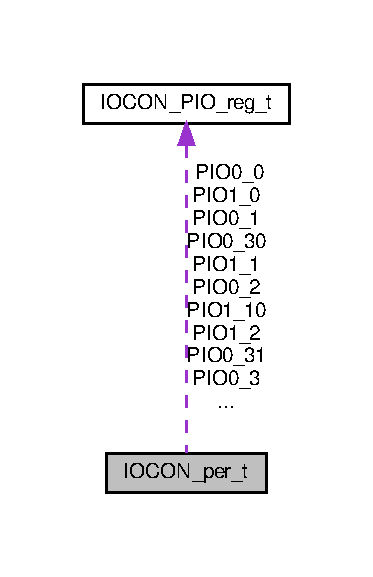
\includegraphics[width=179pt]{structIOCON__per__t__coll__graph}
\end{center}
\end{figure}
\subsection*{Campos de datos}
\begin{DoxyCompactItemize}
\item 
\mbox{\Hypertarget{structIOCON__per__t_a09e974170405c533b8cbaaeff03733c2}\label{structIOCON__per__t_a09e974170405c533b8cbaaeff03733c2}} 
\hyperlink{structIOCON__PIO__reg__t}{I\+O\+C\+O\+N\+\_\+\+P\+I\+O\+\_\+reg\+\_\+t} {\bfseries P\+I\+O0\+\_\+17}
\item 
\mbox{\Hypertarget{structIOCON__per__t_a4ed1689efe380a4459481810cab14360}\label{structIOCON__per__t_a4ed1689efe380a4459481810cab14360}} 
\hyperlink{structIOCON__PIO__reg__t}{I\+O\+C\+O\+N\+\_\+\+P\+I\+O\+\_\+reg\+\_\+t} {\bfseries P\+I\+O0\+\_\+13}
\item 
\mbox{\Hypertarget{structIOCON__per__t_a3e6e4e7c1ab66a1c979dff73b190f3f4}\label{structIOCON__per__t_a3e6e4e7c1ab66a1c979dff73b190f3f4}} 
\hyperlink{structIOCON__PIO__reg__t}{I\+O\+C\+O\+N\+\_\+\+P\+I\+O\+\_\+reg\+\_\+t} {\bfseries P\+I\+O0\+\_\+12}
\item 
\mbox{\Hypertarget{structIOCON__per__t_a2ee4542dfe33025f5cfd31a10648d12f}\label{structIOCON__per__t_a2ee4542dfe33025f5cfd31a10648d12f}} 
\hyperlink{structIOCON__PIO__reg__t}{I\+O\+C\+O\+N\+\_\+\+P\+I\+O\+\_\+reg\+\_\+t} {\bfseries P\+I\+O0\+\_\+5}
\item 
\mbox{\Hypertarget{structIOCON__per__t_a5bcf68e0f9a93019b8a20e14f75f0b8a}\label{structIOCON__per__t_a5bcf68e0f9a93019b8a20e14f75f0b8a}} 
\hyperlink{structIOCON__PIO__reg__t}{I\+O\+C\+O\+N\+\_\+\+P\+I\+O\+\_\+reg\+\_\+t} {\bfseries P\+I\+O0\+\_\+4}
\item 
\mbox{\Hypertarget{structIOCON__per__t_abc6ffeda177ed05d82305a25d1e45736}\label{structIOCON__per__t_abc6ffeda177ed05d82305a25d1e45736}} 
\hyperlink{structIOCON__PIO__reg__t}{I\+O\+C\+O\+N\+\_\+\+P\+I\+O\+\_\+reg\+\_\+t} {\bfseries P\+I\+O0\+\_\+3}
\item 
\mbox{\Hypertarget{structIOCON__per__t_a935f123f3f57ace521e5a6dd03138f1e}\label{structIOCON__per__t_a935f123f3f57ace521e5a6dd03138f1e}} 
\hyperlink{structIOCON__PIO__reg__t}{I\+O\+C\+O\+N\+\_\+\+P\+I\+O\+\_\+reg\+\_\+t} {\bfseries P\+I\+O0\+\_\+2}
\item 
\mbox{\Hypertarget{structIOCON__per__t_ad3c71d25a09f341a30007f20075a954a}\label{structIOCON__per__t_ad3c71d25a09f341a30007f20075a954a}} 
\hyperlink{structIOCON__PIO__reg__t}{I\+O\+C\+O\+N\+\_\+\+P\+I\+O\+\_\+reg\+\_\+t} {\bfseries P\+I\+O0\+\_\+11}
\item 
\mbox{\Hypertarget{structIOCON__per__t_a67a433547c17d7f10646f1cf8d196a84}\label{structIOCON__per__t_a67a433547c17d7f10646f1cf8d196a84}} 
\hyperlink{structIOCON__PIO__reg__t}{I\+O\+C\+O\+N\+\_\+\+P\+I\+O\+\_\+reg\+\_\+t} {\bfseries P\+I\+O0\+\_\+10}
\item 
\mbox{\Hypertarget{structIOCON__per__t_a2f9699bef59ee52b642e3ba0c6620fc3}\label{structIOCON__per__t_a2f9699bef59ee52b642e3ba0c6620fc3}} 
\hyperlink{structIOCON__PIO__reg__t}{I\+O\+C\+O\+N\+\_\+\+P\+I\+O\+\_\+reg\+\_\+t} {\bfseries P\+I\+O0\+\_\+16}
\item 
\mbox{\Hypertarget{structIOCON__per__t_ad9e69b6a60c3506ff7e0d877b035f89a}\label{structIOCON__per__t_ad9e69b6a60c3506ff7e0d877b035f89a}} 
\hyperlink{structIOCON__PIO__reg__t}{I\+O\+C\+O\+N\+\_\+\+P\+I\+O\+\_\+reg\+\_\+t} {\bfseries P\+I\+O0\+\_\+15}
\item 
\mbox{\Hypertarget{structIOCON__per__t_a6744465933d58bc4f34b5f29246b1dc3}\label{structIOCON__per__t_a6744465933d58bc4f34b5f29246b1dc3}} 
\hyperlink{structIOCON__PIO__reg__t}{I\+O\+C\+O\+N\+\_\+\+P\+I\+O\+\_\+reg\+\_\+t} {\bfseries P\+I\+O0\+\_\+1}
\item 
\mbox{\Hypertarget{structIOCON__per__t_aa4290878227db6eb06b7107b145ad363}\label{structIOCON__per__t_aa4290878227db6eb06b7107b145ad363}} 
const uint32\+\_\+t {\bfseries \+\_\+\+R\+E\+S\+E\+R\+V\+E\+D\+\_\+1}
\item 
\mbox{\Hypertarget{structIOCON__per__t_a6b033d132700fee0c62d2f3b725b2f52}\label{structIOCON__per__t_a6b033d132700fee0c62d2f3b725b2f52}} 
\hyperlink{structIOCON__PIO__reg__t}{I\+O\+C\+O\+N\+\_\+\+P\+I\+O\+\_\+reg\+\_\+t} {\bfseries P\+I\+O0\+\_\+9}
\item 
\mbox{\Hypertarget{structIOCON__per__t_acd3127281242df03afa25ce670605f3c}\label{structIOCON__per__t_acd3127281242df03afa25ce670605f3c}} 
\hyperlink{structIOCON__PIO__reg__t}{I\+O\+C\+O\+N\+\_\+\+P\+I\+O\+\_\+reg\+\_\+t} {\bfseries P\+I\+O0\+\_\+8}
\item 
\mbox{\Hypertarget{structIOCON__per__t_a7dfbb761a30632be3f8c56555c15abd0}\label{structIOCON__per__t_a7dfbb761a30632be3f8c56555c15abd0}} 
\hyperlink{structIOCON__PIO__reg__t}{I\+O\+C\+O\+N\+\_\+\+P\+I\+O\+\_\+reg\+\_\+t} {\bfseries P\+I\+O0\+\_\+7}
\item 
\mbox{\Hypertarget{structIOCON__per__t_a17cd083a2f64a81509199779a46a4d4c}\label{structIOCON__per__t_a17cd083a2f64a81509199779a46a4d4c}} 
\hyperlink{structIOCON__PIO__reg__t}{I\+O\+C\+O\+N\+\_\+\+P\+I\+O\+\_\+reg\+\_\+t} {\bfseries P\+I\+O0\+\_\+6}
\item 
\mbox{\Hypertarget{structIOCON__per__t_a8ea3338ddfc6a1f0b11009f9941c3c73}\label{structIOCON__per__t_a8ea3338ddfc6a1f0b11009f9941c3c73}} 
\hyperlink{structIOCON__PIO__reg__t}{I\+O\+C\+O\+N\+\_\+\+P\+I\+O\+\_\+reg\+\_\+t} {\bfseries P\+I\+O0\+\_\+0}
\item 
\mbox{\Hypertarget{structIOCON__per__t_a4938c843657ab4c9936211d6f295285e}\label{structIOCON__per__t_a4938c843657ab4c9936211d6f295285e}} 
\hyperlink{structIOCON__PIO__reg__t}{I\+O\+C\+O\+N\+\_\+\+P\+I\+O\+\_\+reg\+\_\+t} {\bfseries P\+I\+O0\+\_\+14}
\item 
\mbox{\Hypertarget{structIOCON__per__t_ac55d55d5d9a4a3e979f03c57d0ee126a}\label{structIOCON__per__t_ac55d55d5d9a4a3e979f03c57d0ee126a}} 
const uint32\+\_\+t {\bfseries \+\_\+\+R\+E\+S\+E\+R\+V\+E\+D\+\_\+2}
\item 
\mbox{\Hypertarget{structIOCON__per__t_a69f8bf3b5db1eb64c0c157fa96b7c898}\label{structIOCON__per__t_a69f8bf3b5db1eb64c0c157fa96b7c898}} 
\hyperlink{structIOCON__PIO__reg__t}{I\+O\+C\+O\+N\+\_\+\+P\+I\+O\+\_\+reg\+\_\+t} {\bfseries P\+I\+O0\+\_\+28}
\item 
\mbox{\Hypertarget{structIOCON__per__t_ab238e11384dbdad60756d0ee97fa2b4f}\label{structIOCON__per__t_ab238e11384dbdad60756d0ee97fa2b4f}} 
\hyperlink{structIOCON__PIO__reg__t}{I\+O\+C\+O\+N\+\_\+\+P\+I\+O\+\_\+reg\+\_\+t} {\bfseries P\+I\+O0\+\_\+27}
\item 
\mbox{\Hypertarget{structIOCON__per__t_af5a452d3b34c1698a1be41be5fb5dc54}\label{structIOCON__per__t_af5a452d3b34c1698a1be41be5fb5dc54}} 
\hyperlink{structIOCON__PIO__reg__t}{I\+O\+C\+O\+N\+\_\+\+P\+I\+O\+\_\+reg\+\_\+t} {\bfseries P\+I\+O0\+\_\+26}
\item 
\mbox{\Hypertarget{structIOCON__per__t_a07e0deb44605cd0ff776a9204efb1458}\label{structIOCON__per__t_a07e0deb44605cd0ff776a9204efb1458}} 
\hyperlink{structIOCON__PIO__reg__t}{I\+O\+C\+O\+N\+\_\+\+P\+I\+O\+\_\+reg\+\_\+t} {\bfseries P\+I\+O0\+\_\+25}
\item 
\mbox{\Hypertarget{structIOCON__per__t_a1c74155ebfff34976388bbd70303b01e}\label{structIOCON__per__t_a1c74155ebfff34976388bbd70303b01e}} 
\hyperlink{structIOCON__PIO__reg__t}{I\+O\+C\+O\+N\+\_\+\+P\+I\+O\+\_\+reg\+\_\+t} {\bfseries P\+I\+O0\+\_\+24}
\item 
\mbox{\Hypertarget{structIOCON__per__t_ac34b5b544816a8fa5b284cd9f2dd8576}\label{structIOCON__per__t_ac34b5b544816a8fa5b284cd9f2dd8576}} 
\hyperlink{structIOCON__PIO__reg__t}{I\+O\+C\+O\+N\+\_\+\+P\+I\+O\+\_\+reg\+\_\+t} {\bfseries P\+I\+O0\+\_\+23}
\item 
\mbox{\Hypertarget{structIOCON__per__t_ae96e9815a08dab7681c08b7dadeda3d9}\label{structIOCON__per__t_ae96e9815a08dab7681c08b7dadeda3d9}} 
\hyperlink{structIOCON__PIO__reg__t}{I\+O\+C\+O\+N\+\_\+\+P\+I\+O\+\_\+reg\+\_\+t} {\bfseries P\+I\+O0\+\_\+22}
\item 
\mbox{\Hypertarget{structIOCON__per__t_a890ad22a8dda00ffd40508d2b2a280eb}\label{structIOCON__per__t_a890ad22a8dda00ffd40508d2b2a280eb}} 
\hyperlink{structIOCON__PIO__reg__t}{I\+O\+C\+O\+N\+\_\+\+P\+I\+O\+\_\+reg\+\_\+t} {\bfseries P\+I\+O0\+\_\+21}
\item 
\mbox{\Hypertarget{structIOCON__per__t_ad9a0d25f0a945c041f9b9311d8ba3853}\label{structIOCON__per__t_ad9a0d25f0a945c041f9b9311d8ba3853}} 
\hyperlink{structIOCON__PIO__reg__t}{I\+O\+C\+O\+N\+\_\+\+P\+I\+O\+\_\+reg\+\_\+t} {\bfseries P\+I\+O0\+\_\+20}
\item 
\mbox{\Hypertarget{structIOCON__per__t_a916f028569668bbc4d300d75020c0e46}\label{structIOCON__per__t_a916f028569668bbc4d300d75020c0e46}} 
\hyperlink{structIOCON__PIO__reg__t}{I\+O\+C\+O\+N\+\_\+\+P\+I\+O\+\_\+reg\+\_\+t} {\bfseries P\+I\+O0\+\_\+19}
\item 
\mbox{\Hypertarget{structIOCON__per__t_ab1f3caa29501f87f3fcfc3912dfc6ee6}\label{structIOCON__per__t_ab1f3caa29501f87f3fcfc3912dfc6ee6}} 
\hyperlink{structIOCON__PIO__reg__t}{I\+O\+C\+O\+N\+\_\+\+P\+I\+O\+\_\+reg\+\_\+t} {\bfseries P\+I\+O0\+\_\+18}
\item 
\mbox{\Hypertarget{structIOCON__per__t_ac6183c52898c8f76cfa5110249072423}\label{structIOCON__per__t_ac6183c52898c8f76cfa5110249072423}} 
\hyperlink{structIOCON__PIO__reg__t}{I\+O\+C\+O\+N\+\_\+\+P\+I\+O\+\_\+reg\+\_\+t} {\bfseries P\+I\+O1\+\_\+8}
\item 
\mbox{\Hypertarget{structIOCON__per__t_a22747cc3bbb06b52c8d9a2cd931b9b20}\label{structIOCON__per__t_a22747cc3bbb06b52c8d9a2cd931b9b20}} 
\hyperlink{structIOCON__PIO__reg__t}{I\+O\+C\+O\+N\+\_\+\+P\+I\+O\+\_\+reg\+\_\+t} {\bfseries P\+I\+O1\+\_\+9}
\item 
\mbox{\Hypertarget{structIOCON__per__t_af29ff20511462ca2771d4243512251c6}\label{structIOCON__per__t_af29ff20511462ca2771d4243512251c6}} 
\hyperlink{structIOCON__PIO__reg__t}{I\+O\+C\+O\+N\+\_\+\+P\+I\+O\+\_\+reg\+\_\+t} {\bfseries P\+I\+O1\+\_\+12}
\item 
\mbox{\Hypertarget{structIOCON__per__t_a585ecf04f6515335c789901d391fbd70}\label{structIOCON__per__t_a585ecf04f6515335c789901d391fbd70}} 
\hyperlink{structIOCON__PIO__reg__t}{I\+O\+C\+O\+N\+\_\+\+P\+I\+O\+\_\+reg\+\_\+t} {\bfseries P\+I\+O1\+\_\+13}
\item 
\mbox{\Hypertarget{structIOCON__per__t_ace9f1b985a46c5f3b5b538eebff286ed}\label{structIOCON__per__t_ace9f1b985a46c5f3b5b538eebff286ed}} 
\hyperlink{structIOCON__PIO__reg__t}{I\+O\+C\+O\+N\+\_\+\+P\+I\+O\+\_\+reg\+\_\+t} {\bfseries P\+I\+O0\+\_\+31}
\item 
\mbox{\Hypertarget{structIOCON__per__t_ab1bcf4027c54580ec7222df9006bd23a}\label{structIOCON__per__t_ab1bcf4027c54580ec7222df9006bd23a}} 
\hyperlink{structIOCON__PIO__reg__t}{I\+O\+C\+O\+N\+\_\+\+P\+I\+O\+\_\+reg\+\_\+t} {\bfseries P\+I\+O1\+\_\+0}
\item 
\mbox{\Hypertarget{structIOCON__per__t_a5c43c52788984696c8344af75c41f32d}\label{structIOCON__per__t_a5c43c52788984696c8344af75c41f32d}} 
\hyperlink{structIOCON__PIO__reg__t}{I\+O\+C\+O\+N\+\_\+\+P\+I\+O\+\_\+reg\+\_\+t} {\bfseries P\+I\+O1\+\_\+1}
\item 
\mbox{\Hypertarget{structIOCON__per__t_a24d714afc73d95b4be6c5bcf8273dd8f}\label{structIOCON__per__t_a24d714afc73d95b4be6c5bcf8273dd8f}} 
\hyperlink{structIOCON__PIO__reg__t}{I\+O\+C\+O\+N\+\_\+\+P\+I\+O\+\_\+reg\+\_\+t} {\bfseries P\+I\+O1\+\_\+2}
\item 
\mbox{\Hypertarget{structIOCON__per__t_ad3741b938e9150617b51990f22591d5a}\label{structIOCON__per__t_ad3741b938e9150617b51990f22591d5a}} 
\hyperlink{structIOCON__PIO__reg__t}{I\+O\+C\+O\+N\+\_\+\+P\+I\+O\+\_\+reg\+\_\+t} {\bfseries P\+I\+O1\+\_\+14}
\item 
\mbox{\Hypertarget{structIOCON__per__t_a532e9075c8f9785144b0e4c65e5167e1}\label{structIOCON__per__t_a532e9075c8f9785144b0e4c65e5167e1}} 
\hyperlink{structIOCON__PIO__reg__t}{I\+O\+C\+O\+N\+\_\+\+P\+I\+O\+\_\+reg\+\_\+t} {\bfseries P\+I\+O1\+\_\+15}
\item 
\mbox{\Hypertarget{structIOCON__per__t_aba2628e4c4f453738a0594c87dd3be3a}\label{structIOCON__per__t_aba2628e4c4f453738a0594c87dd3be3a}} 
\hyperlink{structIOCON__PIO__reg__t}{I\+O\+C\+O\+N\+\_\+\+P\+I\+O\+\_\+reg\+\_\+t} {\bfseries P\+I\+O1\+\_\+3}
\item 
\mbox{\Hypertarget{structIOCON__per__t_a47628f3a3e2332f593dccfe6f667ac5c}\label{structIOCON__per__t_a47628f3a3e2332f593dccfe6f667ac5c}} 
\hyperlink{structIOCON__PIO__reg__t}{I\+O\+C\+O\+N\+\_\+\+P\+I\+O\+\_\+reg\+\_\+t} {\bfseries P\+I\+O1\+\_\+4}
\item 
\mbox{\Hypertarget{structIOCON__per__t_ae0cb60ca339350f805745199df029d1f}\label{structIOCON__per__t_ae0cb60ca339350f805745199df029d1f}} 
\hyperlink{structIOCON__PIO__reg__t}{I\+O\+C\+O\+N\+\_\+\+P\+I\+O\+\_\+reg\+\_\+t} {\bfseries P\+I\+O1\+\_\+5}
\item 
\mbox{\Hypertarget{structIOCON__per__t_a8187fc08eacc7153cbfb84764891892f}\label{structIOCON__per__t_a8187fc08eacc7153cbfb84764891892f}} 
\hyperlink{structIOCON__PIO__reg__t}{I\+O\+C\+O\+N\+\_\+\+P\+I\+O\+\_\+reg\+\_\+t} {\bfseries P\+I\+O1\+\_\+16}
\item 
\mbox{\Hypertarget{structIOCON__per__t_a074049b1e85c81f10404dd6318c4f3e9}\label{structIOCON__per__t_a074049b1e85c81f10404dd6318c4f3e9}} 
\hyperlink{structIOCON__PIO__reg__t}{I\+O\+C\+O\+N\+\_\+\+P\+I\+O\+\_\+reg\+\_\+t} {\bfseries P\+I\+O1\+\_\+17}
\item 
\mbox{\Hypertarget{structIOCON__per__t_a8427a6d3a276d8ca1043e34bbd7eede8}\label{structIOCON__per__t_a8427a6d3a276d8ca1043e34bbd7eede8}} 
\hyperlink{structIOCON__PIO__reg__t}{I\+O\+C\+O\+N\+\_\+\+P\+I\+O\+\_\+reg\+\_\+t} {\bfseries P\+I\+O1\+\_\+6}
\item 
\mbox{\Hypertarget{structIOCON__per__t_afd0b10b820b078b81694d96cf7463148}\label{structIOCON__per__t_afd0b10b820b078b81694d96cf7463148}} 
\hyperlink{structIOCON__PIO__reg__t}{I\+O\+C\+O\+N\+\_\+\+P\+I\+O\+\_\+reg\+\_\+t} {\bfseries P\+I\+O1\+\_\+18}
\item 
\mbox{\Hypertarget{structIOCON__per__t_af5f3c2b8d31e956f8b12bb4243253a4f}\label{structIOCON__per__t_af5f3c2b8d31e956f8b12bb4243253a4f}} 
\hyperlink{structIOCON__PIO__reg__t}{I\+O\+C\+O\+N\+\_\+\+P\+I\+O\+\_\+reg\+\_\+t} {\bfseries P\+I\+O1\+\_\+19}
\item 
\mbox{\Hypertarget{structIOCON__per__t_a333b8839d321b6fbd2baa7eafa060e2a}\label{structIOCON__per__t_a333b8839d321b6fbd2baa7eafa060e2a}} 
\hyperlink{structIOCON__PIO__reg__t}{I\+O\+C\+O\+N\+\_\+\+P\+I\+O\+\_\+reg\+\_\+t} {\bfseries P\+I\+O1\+\_\+7}
\item 
\mbox{\Hypertarget{structIOCON__per__t_a84b33aa7ed3f8deb291f1512206c93ba}\label{structIOCON__per__t_a84b33aa7ed3f8deb291f1512206c93ba}} 
\hyperlink{structIOCON__PIO__reg__t}{I\+O\+C\+O\+N\+\_\+\+P\+I\+O\+\_\+reg\+\_\+t} {\bfseries P\+I\+O0\+\_\+29}
\item 
\mbox{\Hypertarget{structIOCON__per__t_a904cfdb3dbba5457bfa4d5758bb69550}\label{structIOCON__per__t_a904cfdb3dbba5457bfa4d5758bb69550}} 
\hyperlink{structIOCON__PIO__reg__t}{I\+O\+C\+O\+N\+\_\+\+P\+I\+O\+\_\+reg\+\_\+t} {\bfseries P\+I\+O0\+\_\+30}
\item 
\mbox{\Hypertarget{structIOCON__per__t_a1f782b390ecbc8c7eb7ee909e288dbe9}\label{structIOCON__per__t_a1f782b390ecbc8c7eb7ee909e288dbe9}} 
\hyperlink{structIOCON__PIO__reg__t}{I\+O\+C\+O\+N\+\_\+\+P\+I\+O\+\_\+reg\+\_\+t} {\bfseries P\+I\+O1\+\_\+20}
\item 
\mbox{\Hypertarget{structIOCON__per__t_a015a76e28022f42630219f0e6654dbea}\label{structIOCON__per__t_a015a76e28022f42630219f0e6654dbea}} 
\hyperlink{structIOCON__PIO__reg__t}{I\+O\+C\+O\+N\+\_\+\+P\+I\+O\+\_\+reg\+\_\+t} {\bfseries P\+I\+O1\+\_\+21}
\item 
\mbox{\Hypertarget{structIOCON__per__t_aa93a2042192848cc54fe48993c6bb218}\label{structIOCON__per__t_aa93a2042192848cc54fe48993c6bb218}} 
\hyperlink{structIOCON__PIO__reg__t}{I\+O\+C\+O\+N\+\_\+\+P\+I\+O\+\_\+reg\+\_\+t} {\bfseries P\+I\+O1\+\_\+11}
\item 
\mbox{\Hypertarget{structIOCON__per__t_a837ad45e970ca29519e14d9d4f219cb1}\label{structIOCON__per__t_a837ad45e970ca29519e14d9d4f219cb1}} 
\hyperlink{structIOCON__PIO__reg__t}{I\+O\+C\+O\+N\+\_\+\+P\+I\+O\+\_\+reg\+\_\+t} {\bfseries P\+I\+O1\+\_\+10}
\end{DoxyCompactItemize}


\subsection{Documentación de los campos}
\mbox{\Hypertarget{structIOCON__per__t_a09e974170405c533b8cbaaeff03733c2}\label{structIOCON__per__t_a09e974170405c533b8cbaaeff03733c2}} 
\index{I\+O\+C\+O\+N\+\_\+per\+\_\+t@{I\+O\+C\+O\+N\+\_\+per\+\_\+t}!P\+I\+O0\+\_\+17@{P\+I\+O0\+\_\+17}}
\index{P\+I\+O0\+\_\+17@{P\+I\+O0\+\_\+17}!I\+O\+C\+O\+N\+\_\+per\+\_\+t@{I\+O\+C\+O\+N\+\_\+per\+\_\+t}}
\subsubsection{\texorpdfstring{P\+I\+O0\+\_\+17}{PIO0\_17}}
{\footnotesize\ttfamily \hyperlink{structIOCON__PIO__reg__t}{I\+O\+C\+O\+N\+\_\+\+P\+I\+O\+\_\+reg\+\_\+t} I\+O\+C\+O\+N\+\_\+per\+\_\+t\+::\+P\+I\+O0\+\_\+17}

\mbox{\Hypertarget{structIOCON__per__t_a4ed1689efe380a4459481810cab14360}\label{structIOCON__per__t_a4ed1689efe380a4459481810cab14360}} 
\index{I\+O\+C\+O\+N\+\_\+per\+\_\+t@{I\+O\+C\+O\+N\+\_\+per\+\_\+t}!P\+I\+O0\+\_\+13@{P\+I\+O0\+\_\+13}}
\index{P\+I\+O0\+\_\+13@{P\+I\+O0\+\_\+13}!I\+O\+C\+O\+N\+\_\+per\+\_\+t@{I\+O\+C\+O\+N\+\_\+per\+\_\+t}}
\subsubsection{\texorpdfstring{P\+I\+O0\+\_\+13}{PIO0\_13}}
{\footnotesize\ttfamily \hyperlink{structIOCON__PIO__reg__t}{I\+O\+C\+O\+N\+\_\+\+P\+I\+O\+\_\+reg\+\_\+t} I\+O\+C\+O\+N\+\_\+per\+\_\+t\+::\+P\+I\+O0\+\_\+13}

\mbox{\Hypertarget{structIOCON__per__t_a3e6e4e7c1ab66a1c979dff73b190f3f4}\label{structIOCON__per__t_a3e6e4e7c1ab66a1c979dff73b190f3f4}} 
\index{I\+O\+C\+O\+N\+\_\+per\+\_\+t@{I\+O\+C\+O\+N\+\_\+per\+\_\+t}!P\+I\+O0\+\_\+12@{P\+I\+O0\+\_\+12}}
\index{P\+I\+O0\+\_\+12@{P\+I\+O0\+\_\+12}!I\+O\+C\+O\+N\+\_\+per\+\_\+t@{I\+O\+C\+O\+N\+\_\+per\+\_\+t}}
\subsubsection{\texorpdfstring{P\+I\+O0\+\_\+12}{PIO0\_12}}
{\footnotesize\ttfamily \hyperlink{structIOCON__PIO__reg__t}{I\+O\+C\+O\+N\+\_\+\+P\+I\+O\+\_\+reg\+\_\+t} I\+O\+C\+O\+N\+\_\+per\+\_\+t\+::\+P\+I\+O0\+\_\+12}

\mbox{\Hypertarget{structIOCON__per__t_a2ee4542dfe33025f5cfd31a10648d12f}\label{structIOCON__per__t_a2ee4542dfe33025f5cfd31a10648d12f}} 
\index{I\+O\+C\+O\+N\+\_\+per\+\_\+t@{I\+O\+C\+O\+N\+\_\+per\+\_\+t}!P\+I\+O0\+\_\+5@{P\+I\+O0\+\_\+5}}
\index{P\+I\+O0\+\_\+5@{P\+I\+O0\+\_\+5}!I\+O\+C\+O\+N\+\_\+per\+\_\+t@{I\+O\+C\+O\+N\+\_\+per\+\_\+t}}
\subsubsection{\texorpdfstring{P\+I\+O0\+\_\+5}{PIO0\_5}}
{\footnotesize\ttfamily \hyperlink{structIOCON__PIO__reg__t}{I\+O\+C\+O\+N\+\_\+\+P\+I\+O\+\_\+reg\+\_\+t} I\+O\+C\+O\+N\+\_\+per\+\_\+t\+::\+P\+I\+O0\+\_\+5}

\mbox{\Hypertarget{structIOCON__per__t_a5bcf68e0f9a93019b8a20e14f75f0b8a}\label{structIOCON__per__t_a5bcf68e0f9a93019b8a20e14f75f0b8a}} 
\index{I\+O\+C\+O\+N\+\_\+per\+\_\+t@{I\+O\+C\+O\+N\+\_\+per\+\_\+t}!P\+I\+O0\+\_\+4@{P\+I\+O0\+\_\+4}}
\index{P\+I\+O0\+\_\+4@{P\+I\+O0\+\_\+4}!I\+O\+C\+O\+N\+\_\+per\+\_\+t@{I\+O\+C\+O\+N\+\_\+per\+\_\+t}}
\subsubsection{\texorpdfstring{P\+I\+O0\+\_\+4}{PIO0\_4}}
{\footnotesize\ttfamily \hyperlink{structIOCON__PIO__reg__t}{I\+O\+C\+O\+N\+\_\+\+P\+I\+O\+\_\+reg\+\_\+t} I\+O\+C\+O\+N\+\_\+per\+\_\+t\+::\+P\+I\+O0\+\_\+4}

\mbox{\Hypertarget{structIOCON__per__t_abc6ffeda177ed05d82305a25d1e45736}\label{structIOCON__per__t_abc6ffeda177ed05d82305a25d1e45736}} 
\index{I\+O\+C\+O\+N\+\_\+per\+\_\+t@{I\+O\+C\+O\+N\+\_\+per\+\_\+t}!P\+I\+O0\+\_\+3@{P\+I\+O0\+\_\+3}}
\index{P\+I\+O0\+\_\+3@{P\+I\+O0\+\_\+3}!I\+O\+C\+O\+N\+\_\+per\+\_\+t@{I\+O\+C\+O\+N\+\_\+per\+\_\+t}}
\subsubsection{\texorpdfstring{P\+I\+O0\+\_\+3}{PIO0\_3}}
{\footnotesize\ttfamily \hyperlink{structIOCON__PIO__reg__t}{I\+O\+C\+O\+N\+\_\+\+P\+I\+O\+\_\+reg\+\_\+t} I\+O\+C\+O\+N\+\_\+per\+\_\+t\+::\+P\+I\+O0\+\_\+3}

\mbox{\Hypertarget{structIOCON__per__t_a935f123f3f57ace521e5a6dd03138f1e}\label{structIOCON__per__t_a935f123f3f57ace521e5a6dd03138f1e}} 
\index{I\+O\+C\+O\+N\+\_\+per\+\_\+t@{I\+O\+C\+O\+N\+\_\+per\+\_\+t}!P\+I\+O0\+\_\+2@{P\+I\+O0\+\_\+2}}
\index{P\+I\+O0\+\_\+2@{P\+I\+O0\+\_\+2}!I\+O\+C\+O\+N\+\_\+per\+\_\+t@{I\+O\+C\+O\+N\+\_\+per\+\_\+t}}
\subsubsection{\texorpdfstring{P\+I\+O0\+\_\+2}{PIO0\_2}}
{\footnotesize\ttfamily \hyperlink{structIOCON__PIO__reg__t}{I\+O\+C\+O\+N\+\_\+\+P\+I\+O\+\_\+reg\+\_\+t} I\+O\+C\+O\+N\+\_\+per\+\_\+t\+::\+P\+I\+O0\+\_\+2}

\mbox{\Hypertarget{structIOCON__per__t_ad3c71d25a09f341a30007f20075a954a}\label{structIOCON__per__t_ad3c71d25a09f341a30007f20075a954a}} 
\index{I\+O\+C\+O\+N\+\_\+per\+\_\+t@{I\+O\+C\+O\+N\+\_\+per\+\_\+t}!P\+I\+O0\+\_\+11@{P\+I\+O0\+\_\+11}}
\index{P\+I\+O0\+\_\+11@{P\+I\+O0\+\_\+11}!I\+O\+C\+O\+N\+\_\+per\+\_\+t@{I\+O\+C\+O\+N\+\_\+per\+\_\+t}}
\subsubsection{\texorpdfstring{P\+I\+O0\+\_\+11}{PIO0\_11}}
{\footnotesize\ttfamily \hyperlink{structIOCON__PIO__reg__t}{I\+O\+C\+O\+N\+\_\+\+P\+I\+O\+\_\+reg\+\_\+t} I\+O\+C\+O\+N\+\_\+per\+\_\+t\+::\+P\+I\+O0\+\_\+11}

\mbox{\Hypertarget{structIOCON__per__t_a67a433547c17d7f10646f1cf8d196a84}\label{structIOCON__per__t_a67a433547c17d7f10646f1cf8d196a84}} 
\index{I\+O\+C\+O\+N\+\_\+per\+\_\+t@{I\+O\+C\+O\+N\+\_\+per\+\_\+t}!P\+I\+O0\+\_\+10@{P\+I\+O0\+\_\+10}}
\index{P\+I\+O0\+\_\+10@{P\+I\+O0\+\_\+10}!I\+O\+C\+O\+N\+\_\+per\+\_\+t@{I\+O\+C\+O\+N\+\_\+per\+\_\+t}}
\subsubsection{\texorpdfstring{P\+I\+O0\+\_\+10}{PIO0\_10}}
{\footnotesize\ttfamily \hyperlink{structIOCON__PIO__reg__t}{I\+O\+C\+O\+N\+\_\+\+P\+I\+O\+\_\+reg\+\_\+t} I\+O\+C\+O\+N\+\_\+per\+\_\+t\+::\+P\+I\+O0\+\_\+10}

\mbox{\Hypertarget{structIOCON__per__t_a2f9699bef59ee52b642e3ba0c6620fc3}\label{structIOCON__per__t_a2f9699bef59ee52b642e3ba0c6620fc3}} 
\index{I\+O\+C\+O\+N\+\_\+per\+\_\+t@{I\+O\+C\+O\+N\+\_\+per\+\_\+t}!P\+I\+O0\+\_\+16@{P\+I\+O0\+\_\+16}}
\index{P\+I\+O0\+\_\+16@{P\+I\+O0\+\_\+16}!I\+O\+C\+O\+N\+\_\+per\+\_\+t@{I\+O\+C\+O\+N\+\_\+per\+\_\+t}}
\subsubsection{\texorpdfstring{P\+I\+O0\+\_\+16}{PIO0\_16}}
{\footnotesize\ttfamily \hyperlink{structIOCON__PIO__reg__t}{I\+O\+C\+O\+N\+\_\+\+P\+I\+O\+\_\+reg\+\_\+t} I\+O\+C\+O\+N\+\_\+per\+\_\+t\+::\+P\+I\+O0\+\_\+16}

\mbox{\Hypertarget{structIOCON__per__t_ad9e69b6a60c3506ff7e0d877b035f89a}\label{structIOCON__per__t_ad9e69b6a60c3506ff7e0d877b035f89a}} 
\index{I\+O\+C\+O\+N\+\_\+per\+\_\+t@{I\+O\+C\+O\+N\+\_\+per\+\_\+t}!P\+I\+O0\+\_\+15@{P\+I\+O0\+\_\+15}}
\index{P\+I\+O0\+\_\+15@{P\+I\+O0\+\_\+15}!I\+O\+C\+O\+N\+\_\+per\+\_\+t@{I\+O\+C\+O\+N\+\_\+per\+\_\+t}}
\subsubsection{\texorpdfstring{P\+I\+O0\+\_\+15}{PIO0\_15}}
{\footnotesize\ttfamily \hyperlink{structIOCON__PIO__reg__t}{I\+O\+C\+O\+N\+\_\+\+P\+I\+O\+\_\+reg\+\_\+t} I\+O\+C\+O\+N\+\_\+per\+\_\+t\+::\+P\+I\+O0\+\_\+15}

\mbox{\Hypertarget{structIOCON__per__t_a6744465933d58bc4f34b5f29246b1dc3}\label{structIOCON__per__t_a6744465933d58bc4f34b5f29246b1dc3}} 
\index{I\+O\+C\+O\+N\+\_\+per\+\_\+t@{I\+O\+C\+O\+N\+\_\+per\+\_\+t}!P\+I\+O0\+\_\+1@{P\+I\+O0\+\_\+1}}
\index{P\+I\+O0\+\_\+1@{P\+I\+O0\+\_\+1}!I\+O\+C\+O\+N\+\_\+per\+\_\+t@{I\+O\+C\+O\+N\+\_\+per\+\_\+t}}
\subsubsection{\texorpdfstring{P\+I\+O0\+\_\+1}{PIO0\_1}}
{\footnotesize\ttfamily \hyperlink{structIOCON__PIO__reg__t}{I\+O\+C\+O\+N\+\_\+\+P\+I\+O\+\_\+reg\+\_\+t} I\+O\+C\+O\+N\+\_\+per\+\_\+t\+::\+P\+I\+O0\+\_\+1}

\mbox{\Hypertarget{structIOCON__per__t_aa4290878227db6eb06b7107b145ad363}\label{structIOCON__per__t_aa4290878227db6eb06b7107b145ad363}} 
\index{I\+O\+C\+O\+N\+\_\+per\+\_\+t@{I\+O\+C\+O\+N\+\_\+per\+\_\+t}!\+\_\+\+R\+E\+S\+E\+R\+V\+E\+D\+\_\+1@{\+\_\+\+R\+E\+S\+E\+R\+V\+E\+D\+\_\+1}}
\index{\+\_\+\+R\+E\+S\+E\+R\+V\+E\+D\+\_\+1@{\+\_\+\+R\+E\+S\+E\+R\+V\+E\+D\+\_\+1}!I\+O\+C\+O\+N\+\_\+per\+\_\+t@{I\+O\+C\+O\+N\+\_\+per\+\_\+t}}
\subsubsection{\texorpdfstring{\+\_\+\+R\+E\+S\+E\+R\+V\+E\+D\+\_\+1}{\_RESERVED\_1}}
{\footnotesize\ttfamily const uint32\+\_\+t I\+O\+C\+O\+N\+\_\+per\+\_\+t\+::\+\_\+\+R\+E\+S\+E\+R\+V\+E\+D\+\_\+1}

\mbox{\Hypertarget{structIOCON__per__t_a6b033d132700fee0c62d2f3b725b2f52}\label{structIOCON__per__t_a6b033d132700fee0c62d2f3b725b2f52}} 
\index{I\+O\+C\+O\+N\+\_\+per\+\_\+t@{I\+O\+C\+O\+N\+\_\+per\+\_\+t}!P\+I\+O0\+\_\+9@{P\+I\+O0\+\_\+9}}
\index{P\+I\+O0\+\_\+9@{P\+I\+O0\+\_\+9}!I\+O\+C\+O\+N\+\_\+per\+\_\+t@{I\+O\+C\+O\+N\+\_\+per\+\_\+t}}
\subsubsection{\texorpdfstring{P\+I\+O0\+\_\+9}{PIO0\_9}}
{\footnotesize\ttfamily \hyperlink{structIOCON__PIO__reg__t}{I\+O\+C\+O\+N\+\_\+\+P\+I\+O\+\_\+reg\+\_\+t} I\+O\+C\+O\+N\+\_\+per\+\_\+t\+::\+P\+I\+O0\+\_\+9}

\mbox{\Hypertarget{structIOCON__per__t_acd3127281242df03afa25ce670605f3c}\label{structIOCON__per__t_acd3127281242df03afa25ce670605f3c}} 
\index{I\+O\+C\+O\+N\+\_\+per\+\_\+t@{I\+O\+C\+O\+N\+\_\+per\+\_\+t}!P\+I\+O0\+\_\+8@{P\+I\+O0\+\_\+8}}
\index{P\+I\+O0\+\_\+8@{P\+I\+O0\+\_\+8}!I\+O\+C\+O\+N\+\_\+per\+\_\+t@{I\+O\+C\+O\+N\+\_\+per\+\_\+t}}
\subsubsection{\texorpdfstring{P\+I\+O0\+\_\+8}{PIO0\_8}}
{\footnotesize\ttfamily \hyperlink{structIOCON__PIO__reg__t}{I\+O\+C\+O\+N\+\_\+\+P\+I\+O\+\_\+reg\+\_\+t} I\+O\+C\+O\+N\+\_\+per\+\_\+t\+::\+P\+I\+O0\+\_\+8}

\mbox{\Hypertarget{structIOCON__per__t_a7dfbb761a30632be3f8c56555c15abd0}\label{structIOCON__per__t_a7dfbb761a30632be3f8c56555c15abd0}} 
\index{I\+O\+C\+O\+N\+\_\+per\+\_\+t@{I\+O\+C\+O\+N\+\_\+per\+\_\+t}!P\+I\+O0\+\_\+7@{P\+I\+O0\+\_\+7}}
\index{P\+I\+O0\+\_\+7@{P\+I\+O0\+\_\+7}!I\+O\+C\+O\+N\+\_\+per\+\_\+t@{I\+O\+C\+O\+N\+\_\+per\+\_\+t}}
\subsubsection{\texorpdfstring{P\+I\+O0\+\_\+7}{PIO0\_7}}
{\footnotesize\ttfamily \hyperlink{structIOCON__PIO__reg__t}{I\+O\+C\+O\+N\+\_\+\+P\+I\+O\+\_\+reg\+\_\+t} I\+O\+C\+O\+N\+\_\+per\+\_\+t\+::\+P\+I\+O0\+\_\+7}

\mbox{\Hypertarget{structIOCON__per__t_a17cd083a2f64a81509199779a46a4d4c}\label{structIOCON__per__t_a17cd083a2f64a81509199779a46a4d4c}} 
\index{I\+O\+C\+O\+N\+\_\+per\+\_\+t@{I\+O\+C\+O\+N\+\_\+per\+\_\+t}!P\+I\+O0\+\_\+6@{P\+I\+O0\+\_\+6}}
\index{P\+I\+O0\+\_\+6@{P\+I\+O0\+\_\+6}!I\+O\+C\+O\+N\+\_\+per\+\_\+t@{I\+O\+C\+O\+N\+\_\+per\+\_\+t}}
\subsubsection{\texorpdfstring{P\+I\+O0\+\_\+6}{PIO0\_6}}
{\footnotesize\ttfamily \hyperlink{structIOCON__PIO__reg__t}{I\+O\+C\+O\+N\+\_\+\+P\+I\+O\+\_\+reg\+\_\+t} I\+O\+C\+O\+N\+\_\+per\+\_\+t\+::\+P\+I\+O0\+\_\+6}

\mbox{\Hypertarget{structIOCON__per__t_a8ea3338ddfc6a1f0b11009f9941c3c73}\label{structIOCON__per__t_a8ea3338ddfc6a1f0b11009f9941c3c73}} 
\index{I\+O\+C\+O\+N\+\_\+per\+\_\+t@{I\+O\+C\+O\+N\+\_\+per\+\_\+t}!P\+I\+O0\+\_\+0@{P\+I\+O0\+\_\+0}}
\index{P\+I\+O0\+\_\+0@{P\+I\+O0\+\_\+0}!I\+O\+C\+O\+N\+\_\+per\+\_\+t@{I\+O\+C\+O\+N\+\_\+per\+\_\+t}}
\subsubsection{\texorpdfstring{P\+I\+O0\+\_\+0}{PIO0\_0}}
{\footnotesize\ttfamily \hyperlink{structIOCON__PIO__reg__t}{I\+O\+C\+O\+N\+\_\+\+P\+I\+O\+\_\+reg\+\_\+t} I\+O\+C\+O\+N\+\_\+per\+\_\+t\+::\+P\+I\+O0\+\_\+0}

\mbox{\Hypertarget{structIOCON__per__t_a4938c843657ab4c9936211d6f295285e}\label{structIOCON__per__t_a4938c843657ab4c9936211d6f295285e}} 
\index{I\+O\+C\+O\+N\+\_\+per\+\_\+t@{I\+O\+C\+O\+N\+\_\+per\+\_\+t}!P\+I\+O0\+\_\+14@{P\+I\+O0\+\_\+14}}
\index{P\+I\+O0\+\_\+14@{P\+I\+O0\+\_\+14}!I\+O\+C\+O\+N\+\_\+per\+\_\+t@{I\+O\+C\+O\+N\+\_\+per\+\_\+t}}
\subsubsection{\texorpdfstring{P\+I\+O0\+\_\+14}{PIO0\_14}}
{\footnotesize\ttfamily \hyperlink{structIOCON__PIO__reg__t}{I\+O\+C\+O\+N\+\_\+\+P\+I\+O\+\_\+reg\+\_\+t} I\+O\+C\+O\+N\+\_\+per\+\_\+t\+::\+P\+I\+O0\+\_\+14}

\mbox{\Hypertarget{structIOCON__per__t_ac55d55d5d9a4a3e979f03c57d0ee126a}\label{structIOCON__per__t_ac55d55d5d9a4a3e979f03c57d0ee126a}} 
\index{I\+O\+C\+O\+N\+\_\+per\+\_\+t@{I\+O\+C\+O\+N\+\_\+per\+\_\+t}!\+\_\+\+R\+E\+S\+E\+R\+V\+E\+D\+\_\+2@{\+\_\+\+R\+E\+S\+E\+R\+V\+E\+D\+\_\+2}}
\index{\+\_\+\+R\+E\+S\+E\+R\+V\+E\+D\+\_\+2@{\+\_\+\+R\+E\+S\+E\+R\+V\+E\+D\+\_\+2}!I\+O\+C\+O\+N\+\_\+per\+\_\+t@{I\+O\+C\+O\+N\+\_\+per\+\_\+t}}
\subsubsection{\texorpdfstring{\+\_\+\+R\+E\+S\+E\+R\+V\+E\+D\+\_\+2}{\_RESERVED\_2}}
{\footnotesize\ttfamily const uint32\+\_\+t I\+O\+C\+O\+N\+\_\+per\+\_\+t\+::\+\_\+\+R\+E\+S\+E\+R\+V\+E\+D\+\_\+2}

\mbox{\Hypertarget{structIOCON__per__t_a69f8bf3b5db1eb64c0c157fa96b7c898}\label{structIOCON__per__t_a69f8bf3b5db1eb64c0c157fa96b7c898}} 
\index{I\+O\+C\+O\+N\+\_\+per\+\_\+t@{I\+O\+C\+O\+N\+\_\+per\+\_\+t}!P\+I\+O0\+\_\+28@{P\+I\+O0\+\_\+28}}
\index{P\+I\+O0\+\_\+28@{P\+I\+O0\+\_\+28}!I\+O\+C\+O\+N\+\_\+per\+\_\+t@{I\+O\+C\+O\+N\+\_\+per\+\_\+t}}
\subsubsection{\texorpdfstring{P\+I\+O0\+\_\+28}{PIO0\_28}}
{\footnotesize\ttfamily \hyperlink{structIOCON__PIO__reg__t}{I\+O\+C\+O\+N\+\_\+\+P\+I\+O\+\_\+reg\+\_\+t} I\+O\+C\+O\+N\+\_\+per\+\_\+t\+::\+P\+I\+O0\+\_\+28}

\mbox{\Hypertarget{structIOCON__per__t_ab238e11384dbdad60756d0ee97fa2b4f}\label{structIOCON__per__t_ab238e11384dbdad60756d0ee97fa2b4f}} 
\index{I\+O\+C\+O\+N\+\_\+per\+\_\+t@{I\+O\+C\+O\+N\+\_\+per\+\_\+t}!P\+I\+O0\+\_\+27@{P\+I\+O0\+\_\+27}}
\index{P\+I\+O0\+\_\+27@{P\+I\+O0\+\_\+27}!I\+O\+C\+O\+N\+\_\+per\+\_\+t@{I\+O\+C\+O\+N\+\_\+per\+\_\+t}}
\subsubsection{\texorpdfstring{P\+I\+O0\+\_\+27}{PIO0\_27}}
{\footnotesize\ttfamily \hyperlink{structIOCON__PIO__reg__t}{I\+O\+C\+O\+N\+\_\+\+P\+I\+O\+\_\+reg\+\_\+t} I\+O\+C\+O\+N\+\_\+per\+\_\+t\+::\+P\+I\+O0\+\_\+27}

\mbox{\Hypertarget{structIOCON__per__t_af5a452d3b34c1698a1be41be5fb5dc54}\label{structIOCON__per__t_af5a452d3b34c1698a1be41be5fb5dc54}} 
\index{I\+O\+C\+O\+N\+\_\+per\+\_\+t@{I\+O\+C\+O\+N\+\_\+per\+\_\+t}!P\+I\+O0\+\_\+26@{P\+I\+O0\+\_\+26}}
\index{P\+I\+O0\+\_\+26@{P\+I\+O0\+\_\+26}!I\+O\+C\+O\+N\+\_\+per\+\_\+t@{I\+O\+C\+O\+N\+\_\+per\+\_\+t}}
\subsubsection{\texorpdfstring{P\+I\+O0\+\_\+26}{PIO0\_26}}
{\footnotesize\ttfamily \hyperlink{structIOCON__PIO__reg__t}{I\+O\+C\+O\+N\+\_\+\+P\+I\+O\+\_\+reg\+\_\+t} I\+O\+C\+O\+N\+\_\+per\+\_\+t\+::\+P\+I\+O0\+\_\+26}

\mbox{\Hypertarget{structIOCON__per__t_a07e0deb44605cd0ff776a9204efb1458}\label{structIOCON__per__t_a07e0deb44605cd0ff776a9204efb1458}} 
\index{I\+O\+C\+O\+N\+\_\+per\+\_\+t@{I\+O\+C\+O\+N\+\_\+per\+\_\+t}!P\+I\+O0\+\_\+25@{P\+I\+O0\+\_\+25}}
\index{P\+I\+O0\+\_\+25@{P\+I\+O0\+\_\+25}!I\+O\+C\+O\+N\+\_\+per\+\_\+t@{I\+O\+C\+O\+N\+\_\+per\+\_\+t}}
\subsubsection{\texorpdfstring{P\+I\+O0\+\_\+25}{PIO0\_25}}
{\footnotesize\ttfamily \hyperlink{structIOCON__PIO__reg__t}{I\+O\+C\+O\+N\+\_\+\+P\+I\+O\+\_\+reg\+\_\+t} I\+O\+C\+O\+N\+\_\+per\+\_\+t\+::\+P\+I\+O0\+\_\+25}

\mbox{\Hypertarget{structIOCON__per__t_a1c74155ebfff34976388bbd70303b01e}\label{structIOCON__per__t_a1c74155ebfff34976388bbd70303b01e}} 
\index{I\+O\+C\+O\+N\+\_\+per\+\_\+t@{I\+O\+C\+O\+N\+\_\+per\+\_\+t}!P\+I\+O0\+\_\+24@{P\+I\+O0\+\_\+24}}
\index{P\+I\+O0\+\_\+24@{P\+I\+O0\+\_\+24}!I\+O\+C\+O\+N\+\_\+per\+\_\+t@{I\+O\+C\+O\+N\+\_\+per\+\_\+t}}
\subsubsection{\texorpdfstring{P\+I\+O0\+\_\+24}{PIO0\_24}}
{\footnotesize\ttfamily \hyperlink{structIOCON__PIO__reg__t}{I\+O\+C\+O\+N\+\_\+\+P\+I\+O\+\_\+reg\+\_\+t} I\+O\+C\+O\+N\+\_\+per\+\_\+t\+::\+P\+I\+O0\+\_\+24}

\mbox{\Hypertarget{structIOCON__per__t_ac34b5b544816a8fa5b284cd9f2dd8576}\label{structIOCON__per__t_ac34b5b544816a8fa5b284cd9f2dd8576}} 
\index{I\+O\+C\+O\+N\+\_\+per\+\_\+t@{I\+O\+C\+O\+N\+\_\+per\+\_\+t}!P\+I\+O0\+\_\+23@{P\+I\+O0\+\_\+23}}
\index{P\+I\+O0\+\_\+23@{P\+I\+O0\+\_\+23}!I\+O\+C\+O\+N\+\_\+per\+\_\+t@{I\+O\+C\+O\+N\+\_\+per\+\_\+t}}
\subsubsection{\texorpdfstring{P\+I\+O0\+\_\+23}{PIO0\_23}}
{\footnotesize\ttfamily \hyperlink{structIOCON__PIO__reg__t}{I\+O\+C\+O\+N\+\_\+\+P\+I\+O\+\_\+reg\+\_\+t} I\+O\+C\+O\+N\+\_\+per\+\_\+t\+::\+P\+I\+O0\+\_\+23}

\mbox{\Hypertarget{structIOCON__per__t_ae96e9815a08dab7681c08b7dadeda3d9}\label{structIOCON__per__t_ae96e9815a08dab7681c08b7dadeda3d9}} 
\index{I\+O\+C\+O\+N\+\_\+per\+\_\+t@{I\+O\+C\+O\+N\+\_\+per\+\_\+t}!P\+I\+O0\+\_\+22@{P\+I\+O0\+\_\+22}}
\index{P\+I\+O0\+\_\+22@{P\+I\+O0\+\_\+22}!I\+O\+C\+O\+N\+\_\+per\+\_\+t@{I\+O\+C\+O\+N\+\_\+per\+\_\+t}}
\subsubsection{\texorpdfstring{P\+I\+O0\+\_\+22}{PIO0\_22}}
{\footnotesize\ttfamily \hyperlink{structIOCON__PIO__reg__t}{I\+O\+C\+O\+N\+\_\+\+P\+I\+O\+\_\+reg\+\_\+t} I\+O\+C\+O\+N\+\_\+per\+\_\+t\+::\+P\+I\+O0\+\_\+22}

\mbox{\Hypertarget{structIOCON__per__t_a890ad22a8dda00ffd40508d2b2a280eb}\label{structIOCON__per__t_a890ad22a8dda00ffd40508d2b2a280eb}} 
\index{I\+O\+C\+O\+N\+\_\+per\+\_\+t@{I\+O\+C\+O\+N\+\_\+per\+\_\+t}!P\+I\+O0\+\_\+21@{P\+I\+O0\+\_\+21}}
\index{P\+I\+O0\+\_\+21@{P\+I\+O0\+\_\+21}!I\+O\+C\+O\+N\+\_\+per\+\_\+t@{I\+O\+C\+O\+N\+\_\+per\+\_\+t}}
\subsubsection{\texorpdfstring{P\+I\+O0\+\_\+21}{PIO0\_21}}
{\footnotesize\ttfamily \hyperlink{structIOCON__PIO__reg__t}{I\+O\+C\+O\+N\+\_\+\+P\+I\+O\+\_\+reg\+\_\+t} I\+O\+C\+O\+N\+\_\+per\+\_\+t\+::\+P\+I\+O0\+\_\+21}

\mbox{\Hypertarget{structIOCON__per__t_ad9a0d25f0a945c041f9b9311d8ba3853}\label{structIOCON__per__t_ad9a0d25f0a945c041f9b9311d8ba3853}} 
\index{I\+O\+C\+O\+N\+\_\+per\+\_\+t@{I\+O\+C\+O\+N\+\_\+per\+\_\+t}!P\+I\+O0\+\_\+20@{P\+I\+O0\+\_\+20}}
\index{P\+I\+O0\+\_\+20@{P\+I\+O0\+\_\+20}!I\+O\+C\+O\+N\+\_\+per\+\_\+t@{I\+O\+C\+O\+N\+\_\+per\+\_\+t}}
\subsubsection{\texorpdfstring{P\+I\+O0\+\_\+20}{PIO0\_20}}
{\footnotesize\ttfamily \hyperlink{structIOCON__PIO__reg__t}{I\+O\+C\+O\+N\+\_\+\+P\+I\+O\+\_\+reg\+\_\+t} I\+O\+C\+O\+N\+\_\+per\+\_\+t\+::\+P\+I\+O0\+\_\+20}

\mbox{\Hypertarget{structIOCON__per__t_a916f028569668bbc4d300d75020c0e46}\label{structIOCON__per__t_a916f028569668bbc4d300d75020c0e46}} 
\index{I\+O\+C\+O\+N\+\_\+per\+\_\+t@{I\+O\+C\+O\+N\+\_\+per\+\_\+t}!P\+I\+O0\+\_\+19@{P\+I\+O0\+\_\+19}}
\index{P\+I\+O0\+\_\+19@{P\+I\+O0\+\_\+19}!I\+O\+C\+O\+N\+\_\+per\+\_\+t@{I\+O\+C\+O\+N\+\_\+per\+\_\+t}}
\subsubsection{\texorpdfstring{P\+I\+O0\+\_\+19}{PIO0\_19}}
{\footnotesize\ttfamily \hyperlink{structIOCON__PIO__reg__t}{I\+O\+C\+O\+N\+\_\+\+P\+I\+O\+\_\+reg\+\_\+t} I\+O\+C\+O\+N\+\_\+per\+\_\+t\+::\+P\+I\+O0\+\_\+19}

\mbox{\Hypertarget{structIOCON__per__t_ab1f3caa29501f87f3fcfc3912dfc6ee6}\label{structIOCON__per__t_ab1f3caa29501f87f3fcfc3912dfc6ee6}} 
\index{I\+O\+C\+O\+N\+\_\+per\+\_\+t@{I\+O\+C\+O\+N\+\_\+per\+\_\+t}!P\+I\+O0\+\_\+18@{P\+I\+O0\+\_\+18}}
\index{P\+I\+O0\+\_\+18@{P\+I\+O0\+\_\+18}!I\+O\+C\+O\+N\+\_\+per\+\_\+t@{I\+O\+C\+O\+N\+\_\+per\+\_\+t}}
\subsubsection{\texorpdfstring{P\+I\+O0\+\_\+18}{PIO0\_18}}
{\footnotesize\ttfamily \hyperlink{structIOCON__PIO__reg__t}{I\+O\+C\+O\+N\+\_\+\+P\+I\+O\+\_\+reg\+\_\+t} I\+O\+C\+O\+N\+\_\+per\+\_\+t\+::\+P\+I\+O0\+\_\+18}

\mbox{\Hypertarget{structIOCON__per__t_ac6183c52898c8f76cfa5110249072423}\label{structIOCON__per__t_ac6183c52898c8f76cfa5110249072423}} 
\index{I\+O\+C\+O\+N\+\_\+per\+\_\+t@{I\+O\+C\+O\+N\+\_\+per\+\_\+t}!P\+I\+O1\+\_\+8@{P\+I\+O1\+\_\+8}}
\index{P\+I\+O1\+\_\+8@{P\+I\+O1\+\_\+8}!I\+O\+C\+O\+N\+\_\+per\+\_\+t@{I\+O\+C\+O\+N\+\_\+per\+\_\+t}}
\subsubsection{\texorpdfstring{P\+I\+O1\+\_\+8}{PIO1\_8}}
{\footnotesize\ttfamily \hyperlink{structIOCON__PIO__reg__t}{I\+O\+C\+O\+N\+\_\+\+P\+I\+O\+\_\+reg\+\_\+t} I\+O\+C\+O\+N\+\_\+per\+\_\+t\+::\+P\+I\+O1\+\_\+8}

\mbox{\Hypertarget{structIOCON__per__t_a22747cc3bbb06b52c8d9a2cd931b9b20}\label{structIOCON__per__t_a22747cc3bbb06b52c8d9a2cd931b9b20}} 
\index{I\+O\+C\+O\+N\+\_\+per\+\_\+t@{I\+O\+C\+O\+N\+\_\+per\+\_\+t}!P\+I\+O1\+\_\+9@{P\+I\+O1\+\_\+9}}
\index{P\+I\+O1\+\_\+9@{P\+I\+O1\+\_\+9}!I\+O\+C\+O\+N\+\_\+per\+\_\+t@{I\+O\+C\+O\+N\+\_\+per\+\_\+t}}
\subsubsection{\texorpdfstring{P\+I\+O1\+\_\+9}{PIO1\_9}}
{\footnotesize\ttfamily \hyperlink{structIOCON__PIO__reg__t}{I\+O\+C\+O\+N\+\_\+\+P\+I\+O\+\_\+reg\+\_\+t} I\+O\+C\+O\+N\+\_\+per\+\_\+t\+::\+P\+I\+O1\+\_\+9}

\mbox{\Hypertarget{structIOCON__per__t_af29ff20511462ca2771d4243512251c6}\label{structIOCON__per__t_af29ff20511462ca2771d4243512251c6}} 
\index{I\+O\+C\+O\+N\+\_\+per\+\_\+t@{I\+O\+C\+O\+N\+\_\+per\+\_\+t}!P\+I\+O1\+\_\+12@{P\+I\+O1\+\_\+12}}
\index{P\+I\+O1\+\_\+12@{P\+I\+O1\+\_\+12}!I\+O\+C\+O\+N\+\_\+per\+\_\+t@{I\+O\+C\+O\+N\+\_\+per\+\_\+t}}
\subsubsection{\texorpdfstring{P\+I\+O1\+\_\+12}{PIO1\_12}}
{\footnotesize\ttfamily \hyperlink{structIOCON__PIO__reg__t}{I\+O\+C\+O\+N\+\_\+\+P\+I\+O\+\_\+reg\+\_\+t} I\+O\+C\+O\+N\+\_\+per\+\_\+t\+::\+P\+I\+O1\+\_\+12}

\mbox{\Hypertarget{structIOCON__per__t_a585ecf04f6515335c789901d391fbd70}\label{structIOCON__per__t_a585ecf04f6515335c789901d391fbd70}} 
\index{I\+O\+C\+O\+N\+\_\+per\+\_\+t@{I\+O\+C\+O\+N\+\_\+per\+\_\+t}!P\+I\+O1\+\_\+13@{P\+I\+O1\+\_\+13}}
\index{P\+I\+O1\+\_\+13@{P\+I\+O1\+\_\+13}!I\+O\+C\+O\+N\+\_\+per\+\_\+t@{I\+O\+C\+O\+N\+\_\+per\+\_\+t}}
\subsubsection{\texorpdfstring{P\+I\+O1\+\_\+13}{PIO1\_13}}
{\footnotesize\ttfamily \hyperlink{structIOCON__PIO__reg__t}{I\+O\+C\+O\+N\+\_\+\+P\+I\+O\+\_\+reg\+\_\+t} I\+O\+C\+O\+N\+\_\+per\+\_\+t\+::\+P\+I\+O1\+\_\+13}

\mbox{\Hypertarget{structIOCON__per__t_ace9f1b985a46c5f3b5b538eebff286ed}\label{structIOCON__per__t_ace9f1b985a46c5f3b5b538eebff286ed}} 
\index{I\+O\+C\+O\+N\+\_\+per\+\_\+t@{I\+O\+C\+O\+N\+\_\+per\+\_\+t}!P\+I\+O0\+\_\+31@{P\+I\+O0\+\_\+31}}
\index{P\+I\+O0\+\_\+31@{P\+I\+O0\+\_\+31}!I\+O\+C\+O\+N\+\_\+per\+\_\+t@{I\+O\+C\+O\+N\+\_\+per\+\_\+t}}
\subsubsection{\texorpdfstring{P\+I\+O0\+\_\+31}{PIO0\_31}}
{\footnotesize\ttfamily \hyperlink{structIOCON__PIO__reg__t}{I\+O\+C\+O\+N\+\_\+\+P\+I\+O\+\_\+reg\+\_\+t} I\+O\+C\+O\+N\+\_\+per\+\_\+t\+::\+P\+I\+O0\+\_\+31}

\mbox{\Hypertarget{structIOCON__per__t_ab1bcf4027c54580ec7222df9006bd23a}\label{structIOCON__per__t_ab1bcf4027c54580ec7222df9006bd23a}} 
\index{I\+O\+C\+O\+N\+\_\+per\+\_\+t@{I\+O\+C\+O\+N\+\_\+per\+\_\+t}!P\+I\+O1\+\_\+0@{P\+I\+O1\+\_\+0}}
\index{P\+I\+O1\+\_\+0@{P\+I\+O1\+\_\+0}!I\+O\+C\+O\+N\+\_\+per\+\_\+t@{I\+O\+C\+O\+N\+\_\+per\+\_\+t}}
\subsubsection{\texorpdfstring{P\+I\+O1\+\_\+0}{PIO1\_0}}
{\footnotesize\ttfamily \hyperlink{structIOCON__PIO__reg__t}{I\+O\+C\+O\+N\+\_\+\+P\+I\+O\+\_\+reg\+\_\+t} I\+O\+C\+O\+N\+\_\+per\+\_\+t\+::\+P\+I\+O1\+\_\+0}

\mbox{\Hypertarget{structIOCON__per__t_a5c43c52788984696c8344af75c41f32d}\label{structIOCON__per__t_a5c43c52788984696c8344af75c41f32d}} 
\index{I\+O\+C\+O\+N\+\_\+per\+\_\+t@{I\+O\+C\+O\+N\+\_\+per\+\_\+t}!P\+I\+O1\+\_\+1@{P\+I\+O1\+\_\+1}}
\index{P\+I\+O1\+\_\+1@{P\+I\+O1\+\_\+1}!I\+O\+C\+O\+N\+\_\+per\+\_\+t@{I\+O\+C\+O\+N\+\_\+per\+\_\+t}}
\subsubsection{\texorpdfstring{P\+I\+O1\+\_\+1}{PIO1\_1}}
{\footnotesize\ttfamily \hyperlink{structIOCON__PIO__reg__t}{I\+O\+C\+O\+N\+\_\+\+P\+I\+O\+\_\+reg\+\_\+t} I\+O\+C\+O\+N\+\_\+per\+\_\+t\+::\+P\+I\+O1\+\_\+1}

\mbox{\Hypertarget{structIOCON__per__t_a24d714afc73d95b4be6c5bcf8273dd8f}\label{structIOCON__per__t_a24d714afc73d95b4be6c5bcf8273dd8f}} 
\index{I\+O\+C\+O\+N\+\_\+per\+\_\+t@{I\+O\+C\+O\+N\+\_\+per\+\_\+t}!P\+I\+O1\+\_\+2@{P\+I\+O1\+\_\+2}}
\index{P\+I\+O1\+\_\+2@{P\+I\+O1\+\_\+2}!I\+O\+C\+O\+N\+\_\+per\+\_\+t@{I\+O\+C\+O\+N\+\_\+per\+\_\+t}}
\subsubsection{\texorpdfstring{P\+I\+O1\+\_\+2}{PIO1\_2}}
{\footnotesize\ttfamily \hyperlink{structIOCON__PIO__reg__t}{I\+O\+C\+O\+N\+\_\+\+P\+I\+O\+\_\+reg\+\_\+t} I\+O\+C\+O\+N\+\_\+per\+\_\+t\+::\+P\+I\+O1\+\_\+2}

\mbox{\Hypertarget{structIOCON__per__t_ad3741b938e9150617b51990f22591d5a}\label{structIOCON__per__t_ad3741b938e9150617b51990f22591d5a}} 
\index{I\+O\+C\+O\+N\+\_\+per\+\_\+t@{I\+O\+C\+O\+N\+\_\+per\+\_\+t}!P\+I\+O1\+\_\+14@{P\+I\+O1\+\_\+14}}
\index{P\+I\+O1\+\_\+14@{P\+I\+O1\+\_\+14}!I\+O\+C\+O\+N\+\_\+per\+\_\+t@{I\+O\+C\+O\+N\+\_\+per\+\_\+t}}
\subsubsection{\texorpdfstring{P\+I\+O1\+\_\+14}{PIO1\_14}}
{\footnotesize\ttfamily \hyperlink{structIOCON__PIO__reg__t}{I\+O\+C\+O\+N\+\_\+\+P\+I\+O\+\_\+reg\+\_\+t} I\+O\+C\+O\+N\+\_\+per\+\_\+t\+::\+P\+I\+O1\+\_\+14}

\mbox{\Hypertarget{structIOCON__per__t_a532e9075c8f9785144b0e4c65e5167e1}\label{structIOCON__per__t_a532e9075c8f9785144b0e4c65e5167e1}} 
\index{I\+O\+C\+O\+N\+\_\+per\+\_\+t@{I\+O\+C\+O\+N\+\_\+per\+\_\+t}!P\+I\+O1\+\_\+15@{P\+I\+O1\+\_\+15}}
\index{P\+I\+O1\+\_\+15@{P\+I\+O1\+\_\+15}!I\+O\+C\+O\+N\+\_\+per\+\_\+t@{I\+O\+C\+O\+N\+\_\+per\+\_\+t}}
\subsubsection{\texorpdfstring{P\+I\+O1\+\_\+15}{PIO1\_15}}
{\footnotesize\ttfamily \hyperlink{structIOCON__PIO__reg__t}{I\+O\+C\+O\+N\+\_\+\+P\+I\+O\+\_\+reg\+\_\+t} I\+O\+C\+O\+N\+\_\+per\+\_\+t\+::\+P\+I\+O1\+\_\+15}

\mbox{\Hypertarget{structIOCON__per__t_aba2628e4c4f453738a0594c87dd3be3a}\label{structIOCON__per__t_aba2628e4c4f453738a0594c87dd3be3a}} 
\index{I\+O\+C\+O\+N\+\_\+per\+\_\+t@{I\+O\+C\+O\+N\+\_\+per\+\_\+t}!P\+I\+O1\+\_\+3@{P\+I\+O1\+\_\+3}}
\index{P\+I\+O1\+\_\+3@{P\+I\+O1\+\_\+3}!I\+O\+C\+O\+N\+\_\+per\+\_\+t@{I\+O\+C\+O\+N\+\_\+per\+\_\+t}}
\subsubsection{\texorpdfstring{P\+I\+O1\+\_\+3}{PIO1\_3}}
{\footnotesize\ttfamily \hyperlink{structIOCON__PIO__reg__t}{I\+O\+C\+O\+N\+\_\+\+P\+I\+O\+\_\+reg\+\_\+t} I\+O\+C\+O\+N\+\_\+per\+\_\+t\+::\+P\+I\+O1\+\_\+3}

\mbox{\Hypertarget{structIOCON__per__t_a47628f3a3e2332f593dccfe6f667ac5c}\label{structIOCON__per__t_a47628f3a3e2332f593dccfe6f667ac5c}} 
\index{I\+O\+C\+O\+N\+\_\+per\+\_\+t@{I\+O\+C\+O\+N\+\_\+per\+\_\+t}!P\+I\+O1\+\_\+4@{P\+I\+O1\+\_\+4}}
\index{P\+I\+O1\+\_\+4@{P\+I\+O1\+\_\+4}!I\+O\+C\+O\+N\+\_\+per\+\_\+t@{I\+O\+C\+O\+N\+\_\+per\+\_\+t}}
\subsubsection{\texorpdfstring{P\+I\+O1\+\_\+4}{PIO1\_4}}
{\footnotesize\ttfamily \hyperlink{structIOCON__PIO__reg__t}{I\+O\+C\+O\+N\+\_\+\+P\+I\+O\+\_\+reg\+\_\+t} I\+O\+C\+O\+N\+\_\+per\+\_\+t\+::\+P\+I\+O1\+\_\+4}

\mbox{\Hypertarget{structIOCON__per__t_ae0cb60ca339350f805745199df029d1f}\label{structIOCON__per__t_ae0cb60ca339350f805745199df029d1f}} 
\index{I\+O\+C\+O\+N\+\_\+per\+\_\+t@{I\+O\+C\+O\+N\+\_\+per\+\_\+t}!P\+I\+O1\+\_\+5@{P\+I\+O1\+\_\+5}}
\index{P\+I\+O1\+\_\+5@{P\+I\+O1\+\_\+5}!I\+O\+C\+O\+N\+\_\+per\+\_\+t@{I\+O\+C\+O\+N\+\_\+per\+\_\+t}}
\subsubsection{\texorpdfstring{P\+I\+O1\+\_\+5}{PIO1\_5}}
{\footnotesize\ttfamily \hyperlink{structIOCON__PIO__reg__t}{I\+O\+C\+O\+N\+\_\+\+P\+I\+O\+\_\+reg\+\_\+t} I\+O\+C\+O\+N\+\_\+per\+\_\+t\+::\+P\+I\+O1\+\_\+5}

\mbox{\Hypertarget{structIOCON__per__t_a8187fc08eacc7153cbfb84764891892f}\label{structIOCON__per__t_a8187fc08eacc7153cbfb84764891892f}} 
\index{I\+O\+C\+O\+N\+\_\+per\+\_\+t@{I\+O\+C\+O\+N\+\_\+per\+\_\+t}!P\+I\+O1\+\_\+16@{P\+I\+O1\+\_\+16}}
\index{P\+I\+O1\+\_\+16@{P\+I\+O1\+\_\+16}!I\+O\+C\+O\+N\+\_\+per\+\_\+t@{I\+O\+C\+O\+N\+\_\+per\+\_\+t}}
\subsubsection{\texorpdfstring{P\+I\+O1\+\_\+16}{PIO1\_16}}
{\footnotesize\ttfamily \hyperlink{structIOCON__PIO__reg__t}{I\+O\+C\+O\+N\+\_\+\+P\+I\+O\+\_\+reg\+\_\+t} I\+O\+C\+O\+N\+\_\+per\+\_\+t\+::\+P\+I\+O1\+\_\+16}

\mbox{\Hypertarget{structIOCON__per__t_a074049b1e85c81f10404dd6318c4f3e9}\label{structIOCON__per__t_a074049b1e85c81f10404dd6318c4f3e9}} 
\index{I\+O\+C\+O\+N\+\_\+per\+\_\+t@{I\+O\+C\+O\+N\+\_\+per\+\_\+t}!P\+I\+O1\+\_\+17@{P\+I\+O1\+\_\+17}}
\index{P\+I\+O1\+\_\+17@{P\+I\+O1\+\_\+17}!I\+O\+C\+O\+N\+\_\+per\+\_\+t@{I\+O\+C\+O\+N\+\_\+per\+\_\+t}}
\subsubsection{\texorpdfstring{P\+I\+O1\+\_\+17}{PIO1\_17}}
{\footnotesize\ttfamily \hyperlink{structIOCON__PIO__reg__t}{I\+O\+C\+O\+N\+\_\+\+P\+I\+O\+\_\+reg\+\_\+t} I\+O\+C\+O\+N\+\_\+per\+\_\+t\+::\+P\+I\+O1\+\_\+17}

\mbox{\Hypertarget{structIOCON__per__t_a8427a6d3a276d8ca1043e34bbd7eede8}\label{structIOCON__per__t_a8427a6d3a276d8ca1043e34bbd7eede8}} 
\index{I\+O\+C\+O\+N\+\_\+per\+\_\+t@{I\+O\+C\+O\+N\+\_\+per\+\_\+t}!P\+I\+O1\+\_\+6@{P\+I\+O1\+\_\+6}}
\index{P\+I\+O1\+\_\+6@{P\+I\+O1\+\_\+6}!I\+O\+C\+O\+N\+\_\+per\+\_\+t@{I\+O\+C\+O\+N\+\_\+per\+\_\+t}}
\subsubsection{\texorpdfstring{P\+I\+O1\+\_\+6}{PIO1\_6}}
{\footnotesize\ttfamily \hyperlink{structIOCON__PIO__reg__t}{I\+O\+C\+O\+N\+\_\+\+P\+I\+O\+\_\+reg\+\_\+t} I\+O\+C\+O\+N\+\_\+per\+\_\+t\+::\+P\+I\+O1\+\_\+6}

\mbox{\Hypertarget{structIOCON__per__t_afd0b10b820b078b81694d96cf7463148}\label{structIOCON__per__t_afd0b10b820b078b81694d96cf7463148}} 
\index{I\+O\+C\+O\+N\+\_\+per\+\_\+t@{I\+O\+C\+O\+N\+\_\+per\+\_\+t}!P\+I\+O1\+\_\+18@{P\+I\+O1\+\_\+18}}
\index{P\+I\+O1\+\_\+18@{P\+I\+O1\+\_\+18}!I\+O\+C\+O\+N\+\_\+per\+\_\+t@{I\+O\+C\+O\+N\+\_\+per\+\_\+t}}
\subsubsection{\texorpdfstring{P\+I\+O1\+\_\+18}{PIO1\_18}}
{\footnotesize\ttfamily \hyperlink{structIOCON__PIO__reg__t}{I\+O\+C\+O\+N\+\_\+\+P\+I\+O\+\_\+reg\+\_\+t} I\+O\+C\+O\+N\+\_\+per\+\_\+t\+::\+P\+I\+O1\+\_\+18}

\mbox{\Hypertarget{structIOCON__per__t_af5f3c2b8d31e956f8b12bb4243253a4f}\label{structIOCON__per__t_af5f3c2b8d31e956f8b12bb4243253a4f}} 
\index{I\+O\+C\+O\+N\+\_\+per\+\_\+t@{I\+O\+C\+O\+N\+\_\+per\+\_\+t}!P\+I\+O1\+\_\+19@{P\+I\+O1\+\_\+19}}
\index{P\+I\+O1\+\_\+19@{P\+I\+O1\+\_\+19}!I\+O\+C\+O\+N\+\_\+per\+\_\+t@{I\+O\+C\+O\+N\+\_\+per\+\_\+t}}
\subsubsection{\texorpdfstring{P\+I\+O1\+\_\+19}{PIO1\_19}}
{\footnotesize\ttfamily \hyperlink{structIOCON__PIO__reg__t}{I\+O\+C\+O\+N\+\_\+\+P\+I\+O\+\_\+reg\+\_\+t} I\+O\+C\+O\+N\+\_\+per\+\_\+t\+::\+P\+I\+O1\+\_\+19}

\mbox{\Hypertarget{structIOCON__per__t_a333b8839d321b6fbd2baa7eafa060e2a}\label{structIOCON__per__t_a333b8839d321b6fbd2baa7eafa060e2a}} 
\index{I\+O\+C\+O\+N\+\_\+per\+\_\+t@{I\+O\+C\+O\+N\+\_\+per\+\_\+t}!P\+I\+O1\+\_\+7@{P\+I\+O1\+\_\+7}}
\index{P\+I\+O1\+\_\+7@{P\+I\+O1\+\_\+7}!I\+O\+C\+O\+N\+\_\+per\+\_\+t@{I\+O\+C\+O\+N\+\_\+per\+\_\+t}}
\subsubsection{\texorpdfstring{P\+I\+O1\+\_\+7}{PIO1\_7}}
{\footnotesize\ttfamily \hyperlink{structIOCON__PIO__reg__t}{I\+O\+C\+O\+N\+\_\+\+P\+I\+O\+\_\+reg\+\_\+t} I\+O\+C\+O\+N\+\_\+per\+\_\+t\+::\+P\+I\+O1\+\_\+7}

\mbox{\Hypertarget{structIOCON__per__t_a84b33aa7ed3f8deb291f1512206c93ba}\label{structIOCON__per__t_a84b33aa7ed3f8deb291f1512206c93ba}} 
\index{I\+O\+C\+O\+N\+\_\+per\+\_\+t@{I\+O\+C\+O\+N\+\_\+per\+\_\+t}!P\+I\+O0\+\_\+29@{P\+I\+O0\+\_\+29}}
\index{P\+I\+O0\+\_\+29@{P\+I\+O0\+\_\+29}!I\+O\+C\+O\+N\+\_\+per\+\_\+t@{I\+O\+C\+O\+N\+\_\+per\+\_\+t}}
\subsubsection{\texorpdfstring{P\+I\+O0\+\_\+29}{PIO0\_29}}
{\footnotesize\ttfamily \hyperlink{structIOCON__PIO__reg__t}{I\+O\+C\+O\+N\+\_\+\+P\+I\+O\+\_\+reg\+\_\+t} I\+O\+C\+O\+N\+\_\+per\+\_\+t\+::\+P\+I\+O0\+\_\+29}

\mbox{\Hypertarget{structIOCON__per__t_a904cfdb3dbba5457bfa4d5758bb69550}\label{structIOCON__per__t_a904cfdb3dbba5457bfa4d5758bb69550}} 
\index{I\+O\+C\+O\+N\+\_\+per\+\_\+t@{I\+O\+C\+O\+N\+\_\+per\+\_\+t}!P\+I\+O0\+\_\+30@{P\+I\+O0\+\_\+30}}
\index{P\+I\+O0\+\_\+30@{P\+I\+O0\+\_\+30}!I\+O\+C\+O\+N\+\_\+per\+\_\+t@{I\+O\+C\+O\+N\+\_\+per\+\_\+t}}
\subsubsection{\texorpdfstring{P\+I\+O0\+\_\+30}{PIO0\_30}}
{\footnotesize\ttfamily \hyperlink{structIOCON__PIO__reg__t}{I\+O\+C\+O\+N\+\_\+\+P\+I\+O\+\_\+reg\+\_\+t} I\+O\+C\+O\+N\+\_\+per\+\_\+t\+::\+P\+I\+O0\+\_\+30}

\mbox{\Hypertarget{structIOCON__per__t_a1f782b390ecbc8c7eb7ee909e288dbe9}\label{structIOCON__per__t_a1f782b390ecbc8c7eb7ee909e288dbe9}} 
\index{I\+O\+C\+O\+N\+\_\+per\+\_\+t@{I\+O\+C\+O\+N\+\_\+per\+\_\+t}!P\+I\+O1\+\_\+20@{P\+I\+O1\+\_\+20}}
\index{P\+I\+O1\+\_\+20@{P\+I\+O1\+\_\+20}!I\+O\+C\+O\+N\+\_\+per\+\_\+t@{I\+O\+C\+O\+N\+\_\+per\+\_\+t}}
\subsubsection{\texorpdfstring{P\+I\+O1\+\_\+20}{PIO1\_20}}
{\footnotesize\ttfamily \hyperlink{structIOCON__PIO__reg__t}{I\+O\+C\+O\+N\+\_\+\+P\+I\+O\+\_\+reg\+\_\+t} I\+O\+C\+O\+N\+\_\+per\+\_\+t\+::\+P\+I\+O1\+\_\+20}

\mbox{\Hypertarget{structIOCON__per__t_a015a76e28022f42630219f0e6654dbea}\label{structIOCON__per__t_a015a76e28022f42630219f0e6654dbea}} 
\index{I\+O\+C\+O\+N\+\_\+per\+\_\+t@{I\+O\+C\+O\+N\+\_\+per\+\_\+t}!P\+I\+O1\+\_\+21@{P\+I\+O1\+\_\+21}}
\index{P\+I\+O1\+\_\+21@{P\+I\+O1\+\_\+21}!I\+O\+C\+O\+N\+\_\+per\+\_\+t@{I\+O\+C\+O\+N\+\_\+per\+\_\+t}}
\subsubsection{\texorpdfstring{P\+I\+O1\+\_\+21}{PIO1\_21}}
{\footnotesize\ttfamily \hyperlink{structIOCON__PIO__reg__t}{I\+O\+C\+O\+N\+\_\+\+P\+I\+O\+\_\+reg\+\_\+t} I\+O\+C\+O\+N\+\_\+per\+\_\+t\+::\+P\+I\+O1\+\_\+21}

\mbox{\Hypertarget{structIOCON__per__t_aa93a2042192848cc54fe48993c6bb218}\label{structIOCON__per__t_aa93a2042192848cc54fe48993c6bb218}} 
\index{I\+O\+C\+O\+N\+\_\+per\+\_\+t@{I\+O\+C\+O\+N\+\_\+per\+\_\+t}!P\+I\+O1\+\_\+11@{P\+I\+O1\+\_\+11}}
\index{P\+I\+O1\+\_\+11@{P\+I\+O1\+\_\+11}!I\+O\+C\+O\+N\+\_\+per\+\_\+t@{I\+O\+C\+O\+N\+\_\+per\+\_\+t}}
\subsubsection{\texorpdfstring{P\+I\+O1\+\_\+11}{PIO1\_11}}
{\footnotesize\ttfamily \hyperlink{structIOCON__PIO__reg__t}{I\+O\+C\+O\+N\+\_\+\+P\+I\+O\+\_\+reg\+\_\+t} I\+O\+C\+O\+N\+\_\+per\+\_\+t\+::\+P\+I\+O1\+\_\+11}

\mbox{\Hypertarget{structIOCON__per__t_a837ad45e970ca29519e14d9d4f219cb1}\label{structIOCON__per__t_a837ad45e970ca29519e14d9d4f219cb1}} 
\index{I\+O\+C\+O\+N\+\_\+per\+\_\+t@{I\+O\+C\+O\+N\+\_\+per\+\_\+t}!P\+I\+O1\+\_\+10@{P\+I\+O1\+\_\+10}}
\index{P\+I\+O1\+\_\+10@{P\+I\+O1\+\_\+10}!I\+O\+C\+O\+N\+\_\+per\+\_\+t@{I\+O\+C\+O\+N\+\_\+per\+\_\+t}}
\subsubsection{\texorpdfstring{P\+I\+O1\+\_\+10}{PIO1\_10}}
{\footnotesize\ttfamily \hyperlink{structIOCON__PIO__reg__t}{I\+O\+C\+O\+N\+\_\+\+P\+I\+O\+\_\+reg\+\_\+t} I\+O\+C\+O\+N\+\_\+per\+\_\+t\+::\+P\+I\+O1\+\_\+10}



La documentación para esta estructura fue generada a partir del siguiente fichero\+:\begin{DoxyCompactItemize}
\item 
includes/hri/H\+R\+I\+\_\+\+I\+O\+C\+O\+N.\+h\end{DoxyCompactItemize}

\hypertarget{structIOCON__PIO__reg__t}{}\section{Referencia de la Estructura I\+O\+C\+O\+N\+\_\+\+P\+I\+O\+\_\+reg\+\_\+t}
\label{structIOCON__PIO__reg__t}\index{I\+O\+C\+O\+N\+\_\+\+P\+I\+O\+\_\+reg\+\_\+t@{I\+O\+C\+O\+N\+\_\+\+P\+I\+O\+\_\+reg\+\_\+t}}
\subsection*{Campos de datos}
\begin{DoxyCompactItemize}
\item 
\mbox{\Hypertarget{structIOCON__PIO__reg__t_aa8887a399e416c1f376c227ab1b38ffd}\label{structIOCON__PIO__reg__t_aa8887a399e416c1f376c227ab1b38ffd}} 
uint32\+\_\+t {\bfseries \+\_\+\+\_\+pad0\+\_\+\+\_\+}\+: 3
\item 
\mbox{\Hypertarget{structIOCON__PIO__reg__t_a0560156948d57ae1f2b0c37314462ad4}\label{structIOCON__PIO__reg__t_a0560156948d57ae1f2b0c37314462ad4}} 
uint32\+\_\+t {\bfseries M\+O\+DE}\+: 2
\item 
\mbox{\Hypertarget{structIOCON__PIO__reg__t_a45be45effa1b48ba33eb948051e2a1ac}\label{structIOCON__PIO__reg__t_a45be45effa1b48ba33eb948051e2a1ac}} 
uint32\+\_\+t {\bfseries H\+YS}\+: 1
\item 
\mbox{\Hypertarget{structIOCON__PIO__reg__t_a9bbf121550114db07090cdb5cbafed7e}\label{structIOCON__PIO__reg__t_a9bbf121550114db07090cdb5cbafed7e}} 
uint32\+\_\+t {\bfseries I\+NV}\+: 1
\item 
\mbox{\Hypertarget{structIOCON__PIO__reg__t_a747672ef38d052e84152d871d00fd35f}\label{structIOCON__PIO__reg__t_a747672ef38d052e84152d871d00fd35f}} 
uint32\+\_\+t {\bfseries I2\+C\+M\+O\+DE}\+: 2
\item 
\mbox{\Hypertarget{structIOCON__PIO__reg__t_a34c61348e3b3e08a5162c04a30d50515}\label{structIOCON__PIO__reg__t_a34c61348e3b3e08a5162c04a30d50515}} 
uint32\+\_\+t {\bfseries \+\_\+\+\_\+pad1\+\_\+\+\_\+}\+: 1
\item 
\mbox{\Hypertarget{structIOCON__PIO__reg__t_aa9f648c8f429700919647836a4f8285c}\label{structIOCON__PIO__reg__t_aa9f648c8f429700919647836a4f8285c}} 
uint32\+\_\+t {\bfseries OD}\+: 1
\item 
\mbox{\Hypertarget{structIOCON__PIO__reg__t_a6d9314af10b72ebe0118edb7f0f9d262}\label{structIOCON__PIO__reg__t_a6d9314af10b72ebe0118edb7f0f9d262}} 
uint32\+\_\+t {\bfseries S\+\_\+\+M\+O\+DE}\+: 2
\item 
\mbox{\Hypertarget{structIOCON__PIO__reg__t_ab3884460fab50ee3b82427a8bcdcca7c}\label{structIOCON__PIO__reg__t_ab3884460fab50ee3b82427a8bcdcca7c}} 
uint32\+\_\+t {\bfseries C\+L\+K\+\_\+\+D\+IV}\+: 3
\item 
\mbox{\Hypertarget{structIOCON__PIO__reg__t_a9e26160406dfd46963b66db4ecf829a6}\label{structIOCON__PIO__reg__t_a9e26160406dfd46963b66db4ecf829a6}} 
uint32\+\_\+t {\bfseries D\+A\+C\+M\+O\+DE}\+: 1
\item 
\mbox{\Hypertarget{structIOCON__PIO__reg__t_ab0868bdf2f023282a5d63b39b269abf5}\label{structIOCON__PIO__reg__t_ab0868bdf2f023282a5d63b39b269abf5}} 
uint32\+\_\+t {\bfseries \+\_\+\+\_\+pad2\+\_\+\+\_\+}\+: 15
\end{DoxyCompactItemize}


\subsection{Documentación de los campos}
\mbox{\Hypertarget{structIOCON__PIO__reg__t_aa8887a399e416c1f376c227ab1b38ffd}\label{structIOCON__PIO__reg__t_aa8887a399e416c1f376c227ab1b38ffd}} 
\index{I\+O\+C\+O\+N\+\_\+\+P\+I\+O\+\_\+reg\+\_\+t@{I\+O\+C\+O\+N\+\_\+\+P\+I\+O\+\_\+reg\+\_\+t}!\+\_\+\+\_\+pad0\+\_\+\+\_\+@{\+\_\+\+\_\+pad0\+\_\+\+\_\+}}
\index{\+\_\+\+\_\+pad0\+\_\+\+\_\+@{\+\_\+\+\_\+pad0\+\_\+\+\_\+}!I\+O\+C\+O\+N\+\_\+\+P\+I\+O\+\_\+reg\+\_\+t@{I\+O\+C\+O\+N\+\_\+\+P\+I\+O\+\_\+reg\+\_\+t}}
\subsubsection{\texorpdfstring{\+\_\+\+\_\+pad0\+\_\+\+\_\+}{\_\_pad0\_\_}}
{\footnotesize\ttfamily uint32\+\_\+t I\+O\+C\+O\+N\+\_\+\+P\+I\+O\+\_\+reg\+\_\+t\+::\+\_\+\+\_\+pad0\+\_\+\+\_\+}

\mbox{\Hypertarget{structIOCON__PIO__reg__t_a0560156948d57ae1f2b0c37314462ad4}\label{structIOCON__PIO__reg__t_a0560156948d57ae1f2b0c37314462ad4}} 
\index{I\+O\+C\+O\+N\+\_\+\+P\+I\+O\+\_\+reg\+\_\+t@{I\+O\+C\+O\+N\+\_\+\+P\+I\+O\+\_\+reg\+\_\+t}!M\+O\+DE@{M\+O\+DE}}
\index{M\+O\+DE@{M\+O\+DE}!I\+O\+C\+O\+N\+\_\+\+P\+I\+O\+\_\+reg\+\_\+t@{I\+O\+C\+O\+N\+\_\+\+P\+I\+O\+\_\+reg\+\_\+t}}
\subsubsection{\texorpdfstring{M\+O\+DE}{MODE}}
{\footnotesize\ttfamily uint32\+\_\+t I\+O\+C\+O\+N\+\_\+\+P\+I\+O\+\_\+reg\+\_\+t\+::\+M\+O\+DE}

\mbox{\Hypertarget{structIOCON__PIO__reg__t_a45be45effa1b48ba33eb948051e2a1ac}\label{structIOCON__PIO__reg__t_a45be45effa1b48ba33eb948051e2a1ac}} 
\index{I\+O\+C\+O\+N\+\_\+\+P\+I\+O\+\_\+reg\+\_\+t@{I\+O\+C\+O\+N\+\_\+\+P\+I\+O\+\_\+reg\+\_\+t}!H\+YS@{H\+YS}}
\index{H\+YS@{H\+YS}!I\+O\+C\+O\+N\+\_\+\+P\+I\+O\+\_\+reg\+\_\+t@{I\+O\+C\+O\+N\+\_\+\+P\+I\+O\+\_\+reg\+\_\+t}}
\subsubsection{\texorpdfstring{H\+YS}{HYS}}
{\footnotesize\ttfamily uint32\+\_\+t I\+O\+C\+O\+N\+\_\+\+P\+I\+O\+\_\+reg\+\_\+t\+::\+H\+YS}

\mbox{\Hypertarget{structIOCON__PIO__reg__t_a9bbf121550114db07090cdb5cbafed7e}\label{structIOCON__PIO__reg__t_a9bbf121550114db07090cdb5cbafed7e}} 
\index{I\+O\+C\+O\+N\+\_\+\+P\+I\+O\+\_\+reg\+\_\+t@{I\+O\+C\+O\+N\+\_\+\+P\+I\+O\+\_\+reg\+\_\+t}!I\+NV@{I\+NV}}
\index{I\+NV@{I\+NV}!I\+O\+C\+O\+N\+\_\+\+P\+I\+O\+\_\+reg\+\_\+t@{I\+O\+C\+O\+N\+\_\+\+P\+I\+O\+\_\+reg\+\_\+t}}
\subsubsection{\texorpdfstring{I\+NV}{INV}}
{\footnotesize\ttfamily uint32\+\_\+t I\+O\+C\+O\+N\+\_\+\+P\+I\+O\+\_\+reg\+\_\+t\+::\+I\+NV}

\mbox{\Hypertarget{structIOCON__PIO__reg__t_a747672ef38d052e84152d871d00fd35f}\label{structIOCON__PIO__reg__t_a747672ef38d052e84152d871d00fd35f}} 
\index{I\+O\+C\+O\+N\+\_\+\+P\+I\+O\+\_\+reg\+\_\+t@{I\+O\+C\+O\+N\+\_\+\+P\+I\+O\+\_\+reg\+\_\+t}!I2\+C\+M\+O\+DE@{I2\+C\+M\+O\+DE}}
\index{I2\+C\+M\+O\+DE@{I2\+C\+M\+O\+DE}!I\+O\+C\+O\+N\+\_\+\+P\+I\+O\+\_\+reg\+\_\+t@{I\+O\+C\+O\+N\+\_\+\+P\+I\+O\+\_\+reg\+\_\+t}}
\subsubsection{\texorpdfstring{I2\+C\+M\+O\+DE}{I2CMODE}}
{\footnotesize\ttfamily uint32\+\_\+t I\+O\+C\+O\+N\+\_\+\+P\+I\+O\+\_\+reg\+\_\+t\+::\+I2\+C\+M\+O\+DE}

\mbox{\Hypertarget{structIOCON__PIO__reg__t_a34c61348e3b3e08a5162c04a30d50515}\label{structIOCON__PIO__reg__t_a34c61348e3b3e08a5162c04a30d50515}} 
\index{I\+O\+C\+O\+N\+\_\+\+P\+I\+O\+\_\+reg\+\_\+t@{I\+O\+C\+O\+N\+\_\+\+P\+I\+O\+\_\+reg\+\_\+t}!\+\_\+\+\_\+pad1\+\_\+\+\_\+@{\+\_\+\+\_\+pad1\+\_\+\+\_\+}}
\index{\+\_\+\+\_\+pad1\+\_\+\+\_\+@{\+\_\+\+\_\+pad1\+\_\+\+\_\+}!I\+O\+C\+O\+N\+\_\+\+P\+I\+O\+\_\+reg\+\_\+t@{I\+O\+C\+O\+N\+\_\+\+P\+I\+O\+\_\+reg\+\_\+t}}
\subsubsection{\texorpdfstring{\+\_\+\+\_\+pad1\+\_\+\+\_\+}{\_\_pad1\_\_}}
{\footnotesize\ttfamily uint32\+\_\+t I\+O\+C\+O\+N\+\_\+\+P\+I\+O\+\_\+reg\+\_\+t\+::\+\_\+\+\_\+pad1\+\_\+\+\_\+}

\mbox{\Hypertarget{structIOCON__PIO__reg__t_aa9f648c8f429700919647836a4f8285c}\label{structIOCON__PIO__reg__t_aa9f648c8f429700919647836a4f8285c}} 
\index{I\+O\+C\+O\+N\+\_\+\+P\+I\+O\+\_\+reg\+\_\+t@{I\+O\+C\+O\+N\+\_\+\+P\+I\+O\+\_\+reg\+\_\+t}!OD@{OD}}
\index{OD@{OD}!I\+O\+C\+O\+N\+\_\+\+P\+I\+O\+\_\+reg\+\_\+t@{I\+O\+C\+O\+N\+\_\+\+P\+I\+O\+\_\+reg\+\_\+t}}
\subsubsection{\texorpdfstring{OD}{OD}}
{\footnotesize\ttfamily uint32\+\_\+t I\+O\+C\+O\+N\+\_\+\+P\+I\+O\+\_\+reg\+\_\+t\+::\+OD}

\mbox{\Hypertarget{structIOCON__PIO__reg__t_a6d9314af10b72ebe0118edb7f0f9d262}\label{structIOCON__PIO__reg__t_a6d9314af10b72ebe0118edb7f0f9d262}} 
\index{I\+O\+C\+O\+N\+\_\+\+P\+I\+O\+\_\+reg\+\_\+t@{I\+O\+C\+O\+N\+\_\+\+P\+I\+O\+\_\+reg\+\_\+t}!S\+\_\+\+M\+O\+DE@{S\+\_\+\+M\+O\+DE}}
\index{S\+\_\+\+M\+O\+DE@{S\+\_\+\+M\+O\+DE}!I\+O\+C\+O\+N\+\_\+\+P\+I\+O\+\_\+reg\+\_\+t@{I\+O\+C\+O\+N\+\_\+\+P\+I\+O\+\_\+reg\+\_\+t}}
\subsubsection{\texorpdfstring{S\+\_\+\+M\+O\+DE}{S\_MODE}}
{\footnotesize\ttfamily uint32\+\_\+t I\+O\+C\+O\+N\+\_\+\+P\+I\+O\+\_\+reg\+\_\+t\+::\+S\+\_\+\+M\+O\+DE}

\mbox{\Hypertarget{structIOCON__PIO__reg__t_ab3884460fab50ee3b82427a8bcdcca7c}\label{structIOCON__PIO__reg__t_ab3884460fab50ee3b82427a8bcdcca7c}} 
\index{I\+O\+C\+O\+N\+\_\+\+P\+I\+O\+\_\+reg\+\_\+t@{I\+O\+C\+O\+N\+\_\+\+P\+I\+O\+\_\+reg\+\_\+t}!C\+L\+K\+\_\+\+D\+IV@{C\+L\+K\+\_\+\+D\+IV}}
\index{C\+L\+K\+\_\+\+D\+IV@{C\+L\+K\+\_\+\+D\+IV}!I\+O\+C\+O\+N\+\_\+\+P\+I\+O\+\_\+reg\+\_\+t@{I\+O\+C\+O\+N\+\_\+\+P\+I\+O\+\_\+reg\+\_\+t}}
\subsubsection{\texorpdfstring{C\+L\+K\+\_\+\+D\+IV}{CLK\_DIV}}
{\footnotesize\ttfamily uint32\+\_\+t I\+O\+C\+O\+N\+\_\+\+P\+I\+O\+\_\+reg\+\_\+t\+::\+C\+L\+K\+\_\+\+D\+IV}

\mbox{\Hypertarget{structIOCON__PIO__reg__t_a9e26160406dfd46963b66db4ecf829a6}\label{structIOCON__PIO__reg__t_a9e26160406dfd46963b66db4ecf829a6}} 
\index{I\+O\+C\+O\+N\+\_\+\+P\+I\+O\+\_\+reg\+\_\+t@{I\+O\+C\+O\+N\+\_\+\+P\+I\+O\+\_\+reg\+\_\+t}!D\+A\+C\+M\+O\+DE@{D\+A\+C\+M\+O\+DE}}
\index{D\+A\+C\+M\+O\+DE@{D\+A\+C\+M\+O\+DE}!I\+O\+C\+O\+N\+\_\+\+P\+I\+O\+\_\+reg\+\_\+t@{I\+O\+C\+O\+N\+\_\+\+P\+I\+O\+\_\+reg\+\_\+t}}
\subsubsection{\texorpdfstring{D\+A\+C\+M\+O\+DE}{DACMODE}}
{\footnotesize\ttfamily uint32\+\_\+t I\+O\+C\+O\+N\+\_\+\+P\+I\+O\+\_\+reg\+\_\+t\+::\+D\+A\+C\+M\+O\+DE}

\mbox{\Hypertarget{structIOCON__PIO__reg__t_ab0868bdf2f023282a5d63b39b269abf5}\label{structIOCON__PIO__reg__t_ab0868bdf2f023282a5d63b39b269abf5}} 
\index{I\+O\+C\+O\+N\+\_\+\+P\+I\+O\+\_\+reg\+\_\+t@{I\+O\+C\+O\+N\+\_\+\+P\+I\+O\+\_\+reg\+\_\+t}!\+\_\+\+\_\+pad2\+\_\+\+\_\+@{\+\_\+\+\_\+pad2\+\_\+\+\_\+}}
\index{\+\_\+\+\_\+pad2\+\_\+\+\_\+@{\+\_\+\+\_\+pad2\+\_\+\+\_\+}!I\+O\+C\+O\+N\+\_\+\+P\+I\+O\+\_\+reg\+\_\+t@{I\+O\+C\+O\+N\+\_\+\+P\+I\+O\+\_\+reg\+\_\+t}}
\subsubsection{\texorpdfstring{\+\_\+\+\_\+pad2\+\_\+\+\_\+}{\_\_pad2\_\_}}
{\footnotesize\ttfamily uint32\+\_\+t I\+O\+C\+O\+N\+\_\+\+P\+I\+O\+\_\+reg\+\_\+t\+::\+\_\+\+\_\+pad2\+\_\+\+\_\+}



La documentación para esta estructura fue generada a partir del siguiente fichero\+:\begin{DoxyCompactItemize}
\item 
includes/hri/H\+R\+I\+\_\+\+I\+O\+C\+O\+N.\+h\end{DoxyCompactItemize}

\hypertarget{structtimer__t}{}\section{Referencia de la Estructura timer\+\_\+t}
\label{structtimer__t}\index{timer\+\_\+t@{timer\+\_\+t}}
\subsection*{Campos de datos}
\begin{DoxyCompactItemize}
\item 
\mbox{\Hypertarget{structtimer__t_a9624eaffed5cbcb6266f2207ddaac334}\label{structtimer__t_a9624eaffed5cbcb6266f2207ddaac334}} 
uint8\+\_\+t {\bfseries running}\+: 1
\item 
\mbox{\Hypertarget{structtimer__t_adf4cfba1c8d2514716d4f2b9090a9a88}\label{structtimer__t_adf4cfba1c8d2514716d4f2b9090a9a88}} 
uint8\+\_\+t {\bfseries repeat}\+: 1
\item 
\mbox{\Hypertarget{structtimer__t_a3235adab6714a02d8383ef9e0d5f5e6c}\label{structtimer__t_a3235adab6714a02d8383ef9e0d5f5e6c}} 
uint8\+\_\+t {\bfseries timeouted}\+: 1
\item 
\mbox{\Hypertarget{structtimer__t_ad50a9d39777312284d84d73cccb0fbf9}\label{structtimer__t_ad50a9d39777312284d84d73cccb0fbf9}} 
uint32\+\_\+t {\bfseries msecs}
\item 
\mbox{\Hypertarget{structtimer__t_aa4fd2c575bbe6e4f4b7e4534162ea9b0}\label{structtimer__t_aa4fd2c575bbe6e4f4b7e4534162ea9b0}} 
uint32\+\_\+t {\bfseries msecs\+\_\+to\+\_\+live}
\item 
\mbox{\Hypertarget{structtimer__t_a97cc21c1fc027659274a29e4e4de0200}\label{structtimer__t_a97cc21c1fc027659274a29e4e4de0200}} 
void($\ast$ {\bfseries callback} )(uint8\+\_\+t)
\end{DoxyCompactItemize}


La documentación para esta estructura fue generada a partir del siguiente fichero\+:\begin{DoxyCompactItemize}
\item 
source/infotronic/\hyperlink{timer_8c}{timer.\+c}\end{DoxyCompactItemize}

\chapter{Documentación de archivos}
\hypertarget{HAL__ADC_8h}{}\section{Referencia del Archivo includes/hal/\+H\+A\+L\+\_\+\+A\+DC.h}
\label{HAL__ADC_8h}\index{includes/hal/\+H\+A\+L\+\_\+\+A\+D\+C.\+h@{includes/hal/\+H\+A\+L\+\_\+\+A\+D\+C.\+h}}


Declaraciones a nivel de aplicacion del periferico A\+DC (L\+P\+C845)  


{\ttfamily \#include $<$stdint.\+h$>$}\newline
Dependencia gráfica adjunta para H\+A\+L\+\_\+\+A\+D\+C.\+h\+:\nopagebreak
\begin{figure}[H]
\begin{center}
\leavevmode
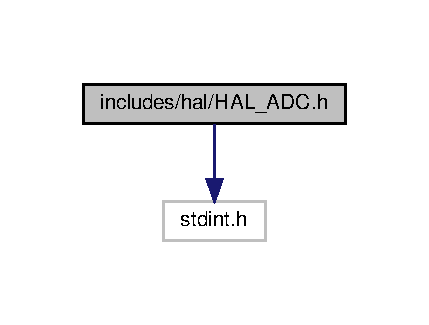
\includegraphics[width=206pt]{HAL__ADC_8h__incl}
\end{center}
\end{figure}
Gráfico de los archivos que directa o indirectamente incluyen a este archivo\+:\nopagebreak
\begin{figure}[H]
\begin{center}
\leavevmode
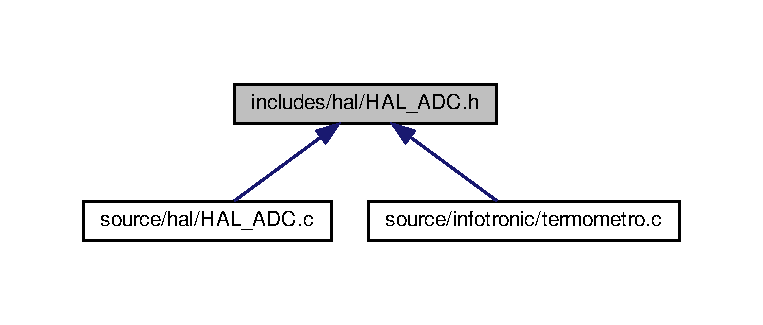
\includegraphics[width=350pt]{HAL__ADC_8h__dep__incl}
\end{center}
\end{figure}
\subsection*{Estructuras de datos}
\begin{DoxyCompactItemize}
\item 
struct \hyperlink{structhal__adc__sequence__config__t}{hal\+\_\+adc\+\_\+sequence\+\_\+config\+\_\+t}
\item 
struct \hyperlink{group__ADC_structhal__adc__sequence__result__t}{hal\+\_\+adc\+\_\+sequence\+\_\+result\+\_\+t}
\end{DoxyCompactItemize}
\subsection*{Enumeraciones}
\begin{DoxyCompactItemize}
\item 
enum \hyperlink{group__ADC_gaee7bd99d368af2a425a9954a9e811a51}{hal\+\_\+adc\+\_\+clock\+\_\+source\+\_\+en} \{ \hyperlink{group__ADC_ggaee7bd99d368af2a425a9954a9e811a51a75a03c616d0b74267642f2b860b19a4c}{H\+A\+L\+\_\+\+A\+D\+C\+\_\+\+C\+L\+O\+C\+K\+\_\+\+S\+O\+U\+R\+C\+E\+\_\+\+F\+RO} = 0, 
\hyperlink{group__ADC_ggaee7bd99d368af2a425a9954a9e811a51ad8be01dc9a2af6e29ab24f823fc40560}{H\+A\+L\+\_\+\+A\+D\+C\+\_\+\+C\+L\+O\+C\+K\+\_\+\+S\+Y\+S\+\_\+\+P\+LL}
 \}
\item 
enum \hyperlink{group__ADC_gaf1570443ca3570a7ae83b90307bbecca}{hal\+\_\+adc\+\_\+low\+\_\+power\+\_\+mode\+\_\+en} \{ \hyperlink{group__ADC_ggaf1570443ca3570a7ae83b90307bbeccaaf92172fb70ce285c23631cb025b3cd52}{H\+A\+L\+\_\+\+A\+D\+C\+\_\+\+L\+O\+W\+\_\+\+P\+O\+W\+E\+R\+\_\+\+M\+O\+D\+E\+\_\+\+D\+I\+S\+A\+B\+L\+ED} = 0, 
\hyperlink{group__ADC_ggaf1570443ca3570a7ae83b90307bbeccaaf3c25521b4c61b46bfe7771db9370769}{H\+A\+L\+\_\+\+A\+D\+C\+\_\+\+L\+O\+W\+\_\+\+P\+O\+W\+E\+R\+\_\+\+M\+O\+D\+E\+\_\+\+E\+N\+A\+B\+L\+ED}
 \}
\item 
enum \hyperlink{group__ADC_ga9297d7b14d7018a94bce94f0103d8559}{hal\+\_\+adc\+\_\+sequence\+\_\+sel\+\_\+en} \{ \hyperlink{group__ADC_gga9297d7b14d7018a94bce94f0103d8559aa8ec9c3fb5a00f2169651f2b1f63df0f}{H\+A\+L\+\_\+\+A\+D\+C\+\_\+\+S\+E\+Q\+U\+E\+N\+C\+E\+\_\+\+S\+E\+L\+\_\+A} = 0, 
\hyperlink{group__ADC_gga9297d7b14d7018a94bce94f0103d8559a109de2c585363efee84dbfb7eee7a1c5}{H\+A\+L\+\_\+\+A\+D\+C\+\_\+\+S\+E\+Q\+U\+E\+N\+C\+E\+\_\+\+S\+E\+L\+\_\+B}
 \}
\item 
enum \hyperlink{group__ADC_ga67fe859b54301579f1b1daef874514ca}{hal\+\_\+adc\+\_\+trigger\+\_\+sel\+\_\+en} \{ \newline
\hyperlink{group__ADC_gga67fe859b54301579f1b1daef874514caaaf722f012bd0aa063b595333f9012a20}{H\+A\+L\+\_\+\+A\+D\+C\+\_\+\+T\+R\+I\+G\+G\+E\+R\+\_\+\+S\+E\+L\+\_\+\+N\+O\+NE} = 0, 
\hyperlink{group__ADC_gga67fe859b54301579f1b1daef874514caa2b6bc8f45ca02b89db9d0b827078a8ac}{H\+A\+L\+\_\+\+A\+D\+C\+\_\+\+T\+R\+I\+G\+G\+E\+R\+\_\+\+S\+E\+L\+\_\+\+P\+I\+N\+I\+N\+T0\+\_\+\+I\+RQ}, 
\hyperlink{group__ADC_gga67fe859b54301579f1b1daef874514caa81102caf42db5f4d5f7b958fe7d9ae6d}{H\+A\+L\+\_\+\+A\+D\+C\+\_\+\+T\+R\+I\+G\+G\+E\+R\+\_\+\+S\+E\+L\+\_\+\+P\+I\+N\+I\+N\+T1\+\_\+\+I\+RQ}, 
\hyperlink{group__ADC_gga67fe859b54301579f1b1daef874514caaca0d6e9551dede7c8a6d596930051e1b}{H\+A\+L\+\_\+\+A\+D\+C\+\_\+\+T\+R\+I\+G\+G\+E\+R\+\_\+\+S\+E\+L\+\_\+\+S\+C\+T0\+\_\+\+O\+U\+T3}, 
\newline
\hyperlink{group__ADC_gga67fe859b54301579f1b1daef874514caabd9e6d4d09caa99ca09a5f44e7797559}{H\+A\+L\+\_\+\+A\+D\+C\+\_\+\+T\+R\+I\+G\+G\+E\+R\+\_\+\+S\+E\+L\+\_\+\+S\+C\+T0\+\_\+\+O\+U\+T4}, 
\hyperlink{group__ADC_gga67fe859b54301579f1b1daef874514caaec235477986c69173f0ad5923a108e5c}{H\+A\+L\+\_\+\+A\+D\+C\+\_\+\+T\+R\+I\+G\+G\+E\+R\+\_\+\+S\+E\+L\+\_\+\+T0\+\_\+\+M\+A\+T3}, 
\hyperlink{group__ADC_gga67fe859b54301579f1b1daef874514caa2ad01d053980af503848525f78d777cf}{H\+A\+L\+\_\+\+A\+D\+C\+\_\+\+T\+R\+I\+G\+G\+E\+R\+\_\+\+S\+E\+L\+\_\+\+C\+M\+P0\+\_\+\+O\+U\+T\+\_\+\+A\+DC}, 
\hyperlink{group__ADC_gga67fe859b54301579f1b1daef874514caa6a9b003480c13c98d8cc1f80bf9c83d1}{H\+A\+L\+\_\+\+A\+D\+C\+\_\+\+T\+R\+I\+G\+G\+E\+R\+\_\+\+S\+E\+L\+\_\+\+G\+P\+I\+O\+\_\+\+I\+N\+T\+\_\+\+B\+M\+AT}, 
\newline
\hyperlink{group__ADC_gga67fe859b54301579f1b1daef874514caa246bfa95b40201277d6c5220c7b57d55}{H\+A\+L\+\_\+\+A\+D\+C\+\_\+\+T\+R\+I\+G\+G\+E\+R\+\_\+\+S\+E\+L\+\_\+\+A\+R\+M\+\_\+\+T\+X\+EV}
 \}
\item 
enum \hyperlink{group__ADC_ga4c5aa9e0991c432640845d2aedb971b2}{hal\+\_\+adc\+\_\+trigger\+\_\+pol\+\_\+sel\+\_\+en} \{ \hyperlink{group__ADC_gga4c5aa9e0991c432640845d2aedb971b2a007c22a34504d8557d98704becf95dc8}{H\+A\+L\+\_\+\+A\+D\+C\+\_\+\+T\+R\+I\+G\+G\+E\+R\+\_\+\+P\+O\+L\+\_\+\+S\+E\+L\+\_\+\+N\+E\+G\+A\+T\+I\+V\+E\+\_\+\+E\+D\+GE} = 0, 
\hyperlink{group__ADC_gga4c5aa9e0991c432640845d2aedb971b2a90868bfab7ec6bdbbca671834798002a}{H\+A\+L\+\_\+\+A\+D\+C\+\_\+\+T\+R\+I\+G\+G\+E\+R\+\_\+\+P\+O\+L\+\_\+\+S\+E\+L\+\_\+\+P\+O\+S\+I\+T\+I\+V\+E\+\_\+\+E\+D\+GE}
 \}
\item 
enum \hyperlink{group__ADC_ga8aa0efd767a9edc5a80b80c4061e0904}{hal\+\_\+adc\+\_\+sync\+\_\+sel\+\_\+en} \{ \hyperlink{group__ADC_gga8aa0efd767a9edc5a80b80c4061e0904a9b81d3ee891639da0e3cec4be09aa668}{H\+A\+L\+\_\+\+A\+D\+C\+\_\+\+S\+Y\+N\+C\+\_\+\+S\+E\+L\+\_\+\+E\+N\+A\+B\+L\+E\+\_\+\+S\+Y\+NC} = 0, 
\hyperlink{group__ADC_gga8aa0efd767a9edc5a80b80c4061e0904a1cbf7646bbe7c32e3e21663fc5952d77}{H\+A\+L\+\_\+\+A\+D\+C\+\_\+\+S\+Y\+N\+C\+\_\+\+S\+E\+L\+\_\+\+B\+Y\+P\+A\+S\+S\+\_\+\+S\+Y\+NC}
 \}
\item 
enum \hyperlink{group__ADC_gaf4981172881d597ede49249ba04fcafe}{hal\+\_\+adc\+\_\+interrupt\+\_\+mode\+\_\+en} \{ \hyperlink{group__ADC_ggaf4981172881d597ede49249ba04fcafea5ffa6da6af1258df4a582e682fab937e}{H\+A\+L\+\_\+\+A\+D\+C\+\_\+\+I\+N\+T\+E\+R\+R\+U\+P\+T\+\_\+\+M\+O\+D\+E\+\_\+\+E\+OC} = 0, 
\hyperlink{group__ADC_ggaf4981172881d597ede49249ba04fcafeae73eff6d5c4ef7297d31a28e4a76e149}{H\+A\+L\+\_\+\+A\+D\+C\+\_\+\+I\+N\+T\+E\+R\+R\+U\+P\+T\+\_\+\+M\+O\+D\+E\+\_\+\+E\+OS}
 \}
\item 
enum \hyperlink{group__ADC_ga99371f47be5b6b4b61c32a1ea86f2b6c}{hal\+\_\+adc\+\_\+result\+\_\+channel\+\_\+en} \{ \newline
\hyperlink{group__ADC_gga99371f47be5b6b4b61c32a1ea86f2b6cae2362f053cdc16412bb073d9b8596c44}{H\+A\+L\+\_\+\+A\+D\+C\+\_\+\+R\+E\+S\+U\+L\+T\+\_\+\+C\+H\+A\+N\+N\+E\+L\+\_\+0} = 0, 
\hyperlink{group__ADC_gga99371f47be5b6b4b61c32a1ea86f2b6cad9342d3898065098fe27e4dcc8a3eb42}{H\+A\+L\+\_\+\+A\+D\+C\+\_\+\+R\+E\+S\+U\+L\+T\+\_\+\+C\+H\+A\+N\+N\+E\+L\+\_\+1}, 
\hyperlink{group__ADC_gga99371f47be5b6b4b61c32a1ea86f2b6ca5d1c958233a386a6c310d9d6a05af99b}{H\+A\+L\+\_\+\+A\+D\+C\+\_\+\+R\+E\+S\+U\+L\+T\+\_\+\+C\+H\+A\+N\+N\+E\+L\+\_\+2}, 
\hyperlink{group__ADC_gga99371f47be5b6b4b61c32a1ea86f2b6ca90074f879325c27fb3e6f3b6457b8cdd}{H\+A\+L\+\_\+\+A\+D\+C\+\_\+\+R\+E\+S\+U\+L\+T\+\_\+\+C\+H\+A\+N\+N\+E\+L\+\_\+3}, 
\newline
\hyperlink{group__ADC_gga99371f47be5b6b4b61c32a1ea86f2b6cad9a84cedc1eb8834223dc1ae6f78f670}{H\+A\+L\+\_\+\+A\+D\+C\+\_\+\+R\+E\+S\+U\+L\+T\+\_\+\+C\+H\+A\+N\+N\+E\+L\+\_\+4}, 
\hyperlink{group__ADC_gga99371f47be5b6b4b61c32a1ea86f2b6cae3c16a8fbe0a0fc75e128f07ba591551}{H\+A\+L\+\_\+\+A\+D\+C\+\_\+\+R\+E\+S\+U\+L\+T\+\_\+\+C\+H\+A\+N\+N\+E\+L\+\_\+5}, 
\hyperlink{group__ADC_gga99371f47be5b6b4b61c32a1ea86f2b6ca9c092202a41a90b27021b181b8095d0c}{H\+A\+L\+\_\+\+A\+D\+C\+\_\+\+R\+E\+S\+U\+L\+T\+\_\+\+C\+H\+A\+N\+N\+E\+L\+\_\+6}, 
\hyperlink{group__ADC_gga99371f47be5b6b4b61c32a1ea86f2b6ca3a9b198659ea511f681900d33c3ba9b5}{H\+A\+L\+\_\+\+A\+D\+C\+\_\+\+R\+E\+S\+U\+L\+T\+\_\+\+C\+H\+A\+N\+N\+E\+L\+\_\+7}, 
\newline
\hyperlink{group__ADC_gga99371f47be5b6b4b61c32a1ea86f2b6cabc4c77b0cea275dd40b1855f82ac6bba}{H\+A\+L\+\_\+\+A\+D\+C\+\_\+\+R\+E\+S\+U\+L\+T\+\_\+\+C\+H\+A\+N\+N\+E\+L\+\_\+8}, 
\hyperlink{group__ADC_gga99371f47be5b6b4b61c32a1ea86f2b6cad33cd49685f140838b575ce39fa26b47}{H\+A\+L\+\_\+\+A\+D\+C\+\_\+\+R\+E\+S\+U\+L\+T\+\_\+\+C\+H\+A\+N\+N\+E\+L\+\_\+9}, 
\hyperlink{group__ADC_gga99371f47be5b6b4b61c32a1ea86f2b6cab81b8df7af28471ac9a6487e88dc0aa8}{H\+A\+L\+\_\+\+A\+D\+C\+\_\+\+R\+E\+S\+U\+L\+T\+\_\+\+C\+H\+A\+N\+N\+E\+L\+\_\+10}, 
\hyperlink{group__ADC_gga99371f47be5b6b4b61c32a1ea86f2b6ca40f8bddc9303b2bae49bb0fcf4dcdf83}{H\+A\+L\+\_\+\+A\+D\+C\+\_\+\+R\+E\+S\+U\+L\+T\+\_\+\+C\+H\+A\+N\+N\+E\+L\+\_\+11}, 
\newline
\hyperlink{group__ADC_gga99371f47be5b6b4b61c32a1ea86f2b6ca5745789eb64375e74e6046b035e92b67}{H\+A\+L\+\_\+\+A\+D\+C\+\_\+\+R\+E\+S\+U\+L\+T\+\_\+\+C\+H\+A\+N\+N\+E\+L\+\_\+\+G\+L\+O\+B\+AL}
 \}
\item 
enum \hyperlink{group__ADC_ga7761986f9c56b809bce1299c6c32eddd}{hal\+\_\+adc\+\_\+sequence\+\_\+result\+\_\+en} \{ \hyperlink{group__ADC_gga7761986f9c56b809bce1299c6c32eddda0c93ff0a1c4ed09ad4b9e1443c4f329f}{H\+A\+L\+\_\+\+A\+D\+C\+\_\+\+S\+E\+Q\+U\+E\+N\+C\+E\+\_\+\+R\+E\+S\+U\+L\+T\+\_\+\+V\+A\+L\+ID} = 0, 
\hyperlink{group__ADC_gga7761986f9c56b809bce1299c6c32edddaec35d0357a3d36bc2c2789d2d45a994e}{H\+A\+L\+\_\+\+A\+D\+C\+\_\+\+S\+E\+Q\+U\+E\+N\+C\+E\+\_\+\+R\+E\+S\+U\+L\+T\+\_\+\+I\+N\+V\+A\+L\+ID}
 \}
\end{DoxyCompactItemize}
\subsection*{Funciones}
\begin{DoxyCompactItemize}
\item 
void \hyperlink{group__ADC_ga4a31179837133973ad68fa993a4e3cd0}{hal\+\_\+adc\+\_\+init\+\_\+async\+\_\+mode} (uint32\+\_\+t sample\+\_\+freq, uint8\+\_\+t div, \hyperlink{group__ADC_gaee7bd99d368af2a425a9954a9e811a51}{hal\+\_\+adc\+\_\+clock\+\_\+source\+\_\+en} clock\+\_\+source, \hyperlink{group__ADC_gaf1570443ca3570a7ae83b90307bbecca}{hal\+\_\+adc\+\_\+low\+\_\+power\+\_\+mode\+\_\+en} low\+\_\+power)
\begin{DoxyCompactList}\small\item\em Inicializar el {\itshape A\+DC} en modo {\bfseries asincrónico}. \end{DoxyCompactList}\item 
void \hyperlink{group__ADC_ga952626700075b275e7766c0095e4ec36}{hal\+\_\+adc\+\_\+init\+\_\+sync\+\_\+mode} (uint32\+\_\+t sample\+\_\+freq, \hyperlink{group__ADC_gaf1570443ca3570a7ae83b90307bbecca}{hal\+\_\+adc\+\_\+low\+\_\+power\+\_\+mode\+\_\+en} low\+\_\+power)
\begin{DoxyCompactList}\small\item\em Inicializar el {\itshape A\+DC} en modo {\bfseries sincrónico}. \end{DoxyCompactList}\item 
void \hyperlink{group__ADC_gab7f00d9f916d45943647ae254ac92d24}{hal\+\_\+adc\+\_\+deinit} (void)
\begin{DoxyCompactList}\small\item\em De-\/inicialización del {\itshape A\+DC}. \end{DoxyCompactList}\item 
void \hyperlink{group__ADC_gadcef726eaa85af74ade96c14f9a48feb}{hal\+\_\+adc\+\_\+config\+\_\+sequence} (\hyperlink{group__ADC_ga9297d7b14d7018a94bce94f0103d8559}{hal\+\_\+adc\+\_\+sequence\+\_\+sel\+\_\+en} sequence, const \hyperlink{structhal__adc__sequence__config__t}{hal\+\_\+adc\+\_\+sequence\+\_\+config\+\_\+t} $\ast$config)
\begin{DoxyCompactList}\small\item\em Configurar una secuencia de conversión. \end{DoxyCompactList}\item 
void \hyperlink{group__ADC_ga678f2df33d79c246b175d0dd36405430}{hal\+\_\+adc\+\_\+enable\+\_\+sequence} (\hyperlink{group__ADC_ga9297d7b14d7018a94bce94f0103d8559}{hal\+\_\+adc\+\_\+sequence\+\_\+sel\+\_\+en} sequence)
\begin{DoxyCompactList}\small\item\em Habilitar una secuencia. \end{DoxyCompactList}\item 
void \hyperlink{group__ADC_ga154950a81b5f589fde0139178ab1dcf3}{hal\+\_\+adc\+\_\+start\+\_\+sequence} (\hyperlink{group__ADC_ga9297d7b14d7018a94bce94f0103d8559}{hal\+\_\+adc\+\_\+sequence\+\_\+sel\+\_\+en} sequence)
\begin{DoxyCompactList}\small\item\em Disparar conversiones en una secuencia. \end{DoxyCompactList}\item 
\hyperlink{group__ADC_ga7761986f9c56b809bce1299c6c32eddd}{hal\+\_\+adc\+\_\+sequence\+\_\+result\+\_\+en} \hyperlink{group__ADC_ga2abe86b92546f8f4726dd65a7a9ddc0d}{hal\+\_\+adc\+\_\+get\+\_\+sequence\+\_\+result} (\hyperlink{group__ADC_ga9297d7b14d7018a94bce94f0103d8559}{hal\+\_\+adc\+\_\+sequence\+\_\+sel\+\_\+en} sequence, \hyperlink{group__ADC_structhal__adc__sequence__result__t}{hal\+\_\+adc\+\_\+sequence\+\_\+result\+\_\+t} $\ast$result\mbox{[}$\,$\mbox{]})
\begin{DoxyCompactList}\small\item\em Obtener resultado de la secuencia. \end{DoxyCompactList}\end{DoxyCompactItemize}


\subsection{Descripción detallada}
Declaraciones a nivel de aplicacion del periferico A\+DC (L\+P\+C845) 

\begin{DoxyAuthor}{Autor}
Augusto Santini 
\end{DoxyAuthor}
\begin{DoxyDate}{Fecha}
3/2020 
\end{DoxyDate}
\begin{DoxyVersion}{Versión}
1.\+0 
\end{DoxyVersion}

\hypertarget{HAL__CTIMER_8h}{}\section{Referencia del Archivo includes/hal/\+H\+A\+L\+\_\+\+C\+T\+I\+M\+ER.h}
\label{HAL__CTIMER_8h}\index{includes/hal/\+H\+A\+L\+\_\+\+C\+T\+I\+M\+E\+R.\+h@{includes/hal/\+H\+A\+L\+\_\+\+C\+T\+I\+M\+E\+R.\+h}}


Declaraciones a nivel de aplicacion del periferico C\+T\+I\+M\+ER (L\+P\+C845)  


{\ttfamily \#include $<$stdint.\+h$>$}\newline
{\ttfamily \#include $<$H\+A\+L\+\_\+\+G\+P\+I\+O.\+h$>$}\newline
Dependencia gráfica adjunta para H\+A\+L\+\_\+\+C\+T\+I\+M\+E\+R.\+h\+:
\nopagebreak
\begin{figure}[H]
\begin{center}
\leavevmode
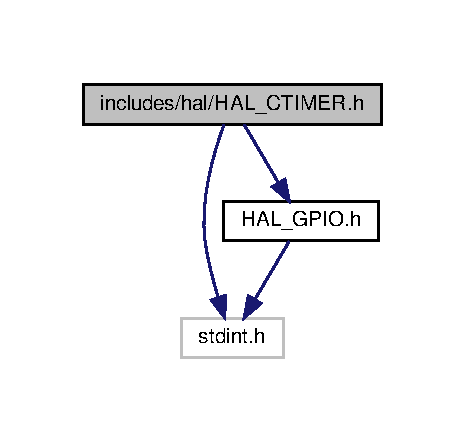
\includegraphics[width=223pt]{HAL__CTIMER_8h__incl}
\end{center}
\end{figure}
\subsection*{Estructuras de datos}
\begin{DoxyCompactItemize}
\item 
struct \hyperlink{structhal__ctimer__match__config__t}{hal\+\_\+ctimer\+\_\+match\+\_\+config\+\_\+t}
\item 
struct \hyperlink{structhal__ctimer__pwm__channel__config__t}{hal\+\_\+ctimer\+\_\+pwm\+\_\+channel\+\_\+config\+\_\+t}
\item 
struct \hyperlink{structhal__ctimer__pwm__config__t}{hal\+\_\+ctimer\+\_\+pwm\+\_\+config\+\_\+t}
\end{DoxyCompactItemize}
\subsection*{Enumeraciones}
\begin{DoxyCompactItemize}
\item 
\mbox{\Hypertarget{HAL__CTIMER_8h_a6aaedba4bb4587f2eacf9e37d4d164bf}\label{HAL__CTIMER_8h_a6aaedba4bb4587f2eacf9e37d4d164bf}} 
enum {\bfseries hal\+\_\+ctimer\+\_\+match\+\_\+action\+\_\+en} \{ {\bfseries H\+A\+L\+\_\+\+C\+T\+I\+M\+E\+R\+\_\+\+M\+A\+T\+C\+H\+\_\+\+D\+O\+\_\+\+N\+O\+G\+H\+I\+NG} = 0, 
{\bfseries H\+A\+L\+\_\+\+C\+T\+I\+M\+E\+R\+\_\+\+M\+A\+T\+C\+H\+\_\+\+C\+L\+E\+A\+R\+\_\+\+P\+IN}, 
{\bfseries H\+A\+L\+\_\+\+C\+T\+I\+M\+E\+R\+\_\+\+M\+A\+T\+C\+H\+\_\+\+S\+E\+T\+\_\+\+P\+IN}, 
{\bfseries H\+A\+L\+\_\+\+C\+T\+I\+M\+E\+R\+\_\+\+M\+A\+T\+C\+H\+\_\+\+T\+O\+G\+G\+L\+E\+\_\+\+P\+IN}
 \}
\item 
\mbox{\Hypertarget{HAL__CTIMER_8h_aeb49458e605ad9b4591fc0a367df2f3f}\label{HAL__CTIMER_8h_aeb49458e605ad9b4591fc0a367df2f3f}} 
enum {\bfseries hal\+\_\+ctimer\+\_\+match\+\_\+sel\+\_\+en} \{ {\bfseries H\+A\+L\+\_\+\+C\+T\+I\+M\+E\+R\+\_\+\+M\+A\+T\+C\+H\+\_\+0} = 0, 
{\bfseries H\+A\+L\+\_\+\+C\+T\+I\+M\+E\+R\+\_\+\+M\+A\+T\+C\+H\+\_\+1}, 
{\bfseries H\+A\+L\+\_\+\+C\+T\+I\+M\+E\+R\+\_\+\+M\+A\+T\+C\+H\+\_\+2}, 
{\bfseries H\+A\+L\+\_\+\+C\+T\+I\+M\+E\+R\+\_\+\+M\+A\+T\+C\+H\+\_\+3}
 \}
\item 
\mbox{\Hypertarget{HAL__CTIMER_8h_a96a7ca81e59a07810e0f9450b9daa8c1}\label{HAL__CTIMER_8h_a96a7ca81e59a07810e0f9450b9daa8c1}} 
enum {\bfseries hal\+\_\+ctimer\+\_\+pwm\+\_\+channel\+\_\+sel\+\_\+en} \{ {\bfseries H\+A\+L\+\_\+\+C\+T\+I\+M\+E\+R\+\_\+\+P\+W\+M\+\_\+\+C\+H\+A\+N\+N\+E\+L\+\_\+0} = 0, 
{\bfseries H\+A\+L\+\_\+\+C\+T\+I\+M\+E\+R\+\_\+\+P\+W\+M\+\_\+\+C\+H\+A\+N\+N\+E\+L\+\_\+1}, 
{\bfseries H\+A\+L\+\_\+\+C\+T\+I\+M\+E\+R\+\_\+\+P\+W\+M\+\_\+\+C\+H\+A\+N\+N\+E\+L\+\_\+2}
 \}
\end{DoxyCompactItemize}
\subsection*{Funciones}
\begin{DoxyCompactItemize}
\item 
void \hyperlink{HAL__CTIMER_8h_a4689eed2a9e77b21de79cc9c9769e269}{hal\+\_\+ctimer\+\_\+timer\+\_\+mode\+\_\+init} (uint32\+\_\+t clock\+\_\+div)
\begin{DoxyCompactList}\small\item\em Inicializacion del periferico en modo timer. \end{DoxyCompactList}\item 
void \hyperlink{HAL__CTIMER_8h_a2a68e905c8f05c550bf06e34f4a1484e}{hal\+\_\+ctimer\+\_\+timer\+\_\+mode\+\_\+config\+\_\+match} (hal\+\_\+ctimer\+\_\+match\+\_\+sel\+\_\+en match\+\_\+sel, const \hyperlink{structhal__ctimer__match__config__t}{hal\+\_\+ctimer\+\_\+match\+\_\+config\+\_\+t} $\ast$match\+\_\+config)
\begin{DoxyCompactList}\small\item\em Configurar un canal de match. \end{DoxyCompactList}\item 
\mbox{\Hypertarget{HAL__CTIMER_8h_a803fbca6afb0855021986d204ffa4b9f}\label{HAL__CTIMER_8h_a803fbca6afb0855021986d204ffa4b9f}} 
void \hyperlink{HAL__CTIMER_8h_a803fbca6afb0855021986d204ffa4b9f}{hal\+\_\+ctimer\+\_\+timer\+\_\+mode\+\_\+run} (void)
\begin{DoxyCompactList}\small\item\em Habilitar el conteo del ctimer. \end{DoxyCompactList}\item 
\mbox{\Hypertarget{HAL__CTIMER_8h_ad855b264d39d920aee8be3c9a0a37db6}\label{HAL__CTIMER_8h_ad855b264d39d920aee8be3c9a0a37db6}} 
void \hyperlink{HAL__CTIMER_8h_ad855b264d39d920aee8be3c9a0a37db6}{hal\+\_\+ctimer\+\_\+timer\+\_\+mode\+\_\+stop} (void)
\begin{DoxyCompactList}\small\item\em Inhabilitar el conteo del ctimer. \end{DoxyCompactList}\item 
\mbox{\Hypertarget{HAL__CTIMER_8h_adc1257569aeffe26a73a3f1af6417d12}\label{HAL__CTIMER_8h_adc1257569aeffe26a73a3f1af6417d12}} 
void \hyperlink{HAL__CTIMER_8h_adc1257569aeffe26a73a3f1af6417d12}{hal\+\_\+ctimer\+\_\+timer\+\_\+mode\+\_\+reset} (void)
\begin{DoxyCompactList}\small\item\em Reiniciar el conteo del ctimer. \end{DoxyCompactList}\item 
void \hyperlink{HAL__CTIMER_8h_a1629367b79d8b3e0fb2769e0b2b96e9c}{hal\+\_\+ctimer\+\_\+pwm\+\_\+mode\+\_\+init} (const \hyperlink{structhal__ctimer__pwm__config__t}{hal\+\_\+ctimer\+\_\+pwm\+\_\+config\+\_\+t} $\ast$config)
\begin{DoxyCompactList}\small\item\em Inicializar el C\+T\+I\+M\+ER en modo P\+WM. \end{DoxyCompactList}\item 
void \hyperlink{HAL__CTIMER_8h_a722302303f22f47995cc6d48bfa1533f}{hal\+\_\+ctimer\+\_\+pwm\+\_\+mode\+\_\+set\+\_\+period} (uint32\+\_\+t period\+\_\+useg)
\begin{DoxyCompactList}\small\item\em Actualizar el periodo en modo P\+WM. \end{DoxyCompactList}\item 
void \hyperlink{HAL__CTIMER_8h_a767f590f1745869d37f7d94a7873280b}{hal\+\_\+ctimer\+\_\+pwm\+\_\+mode\+\_\+config\+\_\+channel} (hal\+\_\+ctimer\+\_\+pwm\+\_\+channel\+\_\+sel\+\_\+en channel\+\_\+sel, const \hyperlink{structhal__ctimer__pwm__channel__config__t}{hal\+\_\+ctimer\+\_\+pwm\+\_\+channel\+\_\+config\+\_\+t} $\ast$channel\+\_\+config)
\begin{DoxyCompactList}\small\item\em Actualizar configuracion de algun canal de P\+WM. \end{DoxyCompactList}\end{DoxyCompactItemize}


\subsection{Descripción detallada}
Declaraciones a nivel de aplicacion del periferico C\+T\+I\+M\+ER (L\+P\+C845) 

\begin{DoxyAuthor}{Autor}
Augusto Santini 
\end{DoxyAuthor}
\begin{DoxyDate}{Fecha}
3/2020 
\end{DoxyDate}
\begin{DoxyVersion}{Versión}
1.\+0 
\end{DoxyVersion}


\subsection{Documentación de las funciones}
\mbox{\Hypertarget{HAL__CTIMER_8h_a4689eed2a9e77b21de79cc9c9769e269}\label{HAL__CTIMER_8h_a4689eed2a9e77b21de79cc9c9769e269}} 
\index{H\+A\+L\+\_\+\+C\+T\+I\+M\+E\+R.\+h@{H\+A\+L\+\_\+\+C\+T\+I\+M\+E\+R.\+h}!hal\+\_\+ctimer\+\_\+timer\+\_\+mode\+\_\+init@{hal\+\_\+ctimer\+\_\+timer\+\_\+mode\+\_\+init}}
\index{hal\+\_\+ctimer\+\_\+timer\+\_\+mode\+\_\+init@{hal\+\_\+ctimer\+\_\+timer\+\_\+mode\+\_\+init}!H\+A\+L\+\_\+\+C\+T\+I\+M\+E\+R.\+h@{H\+A\+L\+\_\+\+C\+T\+I\+M\+E\+R.\+h}}
\subsubsection{\texorpdfstring{hal\+\_\+ctimer\+\_\+timer\+\_\+mode\+\_\+init()}{hal\_ctimer\_timer\_mode\_init()}}
{\footnotesize\ttfamily void hal\+\_\+ctimer\+\_\+timer\+\_\+mode\+\_\+init (\begin{DoxyParamCaption}\item[{uint32\+\_\+t}]{clock\+\_\+div }\end{DoxyParamCaption})}



Inicializacion del periferico en modo timer. 

Esta funcion no pone a correr el contador.


\begin{DoxyParams}[1]{Parámetros}
\mbox{\tt in}  & {\em clock\+\_\+div} & Divisor del clock principal deseado (el valor efectivo es este valor + 1) \\
\hline
\end{DoxyParams}
\mbox{\Hypertarget{HAL__CTIMER_8h_a2a68e905c8f05c550bf06e34f4a1484e}\label{HAL__CTIMER_8h_a2a68e905c8f05c550bf06e34f4a1484e}} 
\index{H\+A\+L\+\_\+\+C\+T\+I\+M\+E\+R.\+h@{H\+A\+L\+\_\+\+C\+T\+I\+M\+E\+R.\+h}!hal\+\_\+ctimer\+\_\+timer\+\_\+mode\+\_\+config\+\_\+match@{hal\+\_\+ctimer\+\_\+timer\+\_\+mode\+\_\+config\+\_\+match}}
\index{hal\+\_\+ctimer\+\_\+timer\+\_\+mode\+\_\+config\+\_\+match@{hal\+\_\+ctimer\+\_\+timer\+\_\+mode\+\_\+config\+\_\+match}!H\+A\+L\+\_\+\+C\+T\+I\+M\+E\+R.\+h@{H\+A\+L\+\_\+\+C\+T\+I\+M\+E\+R.\+h}}
\subsubsection{\texorpdfstring{hal\+\_\+ctimer\+\_\+timer\+\_\+mode\+\_\+config\+\_\+match()}{hal\_ctimer\_timer\_mode\_config\_match()}}
{\footnotesize\ttfamily void hal\+\_\+ctimer\+\_\+timer\+\_\+mode\+\_\+config\+\_\+match (\begin{DoxyParamCaption}\item[{hal\+\_\+ctimer\+\_\+match\+\_\+sel\+\_\+en}]{match\+\_\+sel,  }\item[{const \hyperlink{structhal__ctimer__match__config__t}{hal\+\_\+ctimer\+\_\+match\+\_\+config\+\_\+t} $\ast$}]{match\+\_\+config }\end{DoxyParamCaption})}



Configurar un canal de match. 


\begin{DoxyParams}[1]{Parámetros}
\mbox{\tt in}  & {\em match\+\_\+sel} & Match a configurar \\
\hline
\mbox{\tt in}  & {\em match\+\_\+config} & Configuracion deseada \\
\hline
\end{DoxyParams}
\mbox{\Hypertarget{HAL__CTIMER_8h_a1629367b79d8b3e0fb2769e0b2b96e9c}\label{HAL__CTIMER_8h_a1629367b79d8b3e0fb2769e0b2b96e9c}} 
\index{H\+A\+L\+\_\+\+C\+T\+I\+M\+E\+R.\+h@{H\+A\+L\+\_\+\+C\+T\+I\+M\+E\+R.\+h}!hal\+\_\+ctimer\+\_\+pwm\+\_\+mode\+\_\+init@{hal\+\_\+ctimer\+\_\+pwm\+\_\+mode\+\_\+init}}
\index{hal\+\_\+ctimer\+\_\+pwm\+\_\+mode\+\_\+init@{hal\+\_\+ctimer\+\_\+pwm\+\_\+mode\+\_\+init}!H\+A\+L\+\_\+\+C\+T\+I\+M\+E\+R.\+h@{H\+A\+L\+\_\+\+C\+T\+I\+M\+E\+R.\+h}}
\subsubsection{\texorpdfstring{hal\+\_\+ctimer\+\_\+pwm\+\_\+mode\+\_\+init()}{hal\_ctimer\_pwm\_mode\_init()}}
{\footnotesize\ttfamily void hal\+\_\+ctimer\+\_\+pwm\+\_\+mode\+\_\+init (\begin{DoxyParamCaption}\item[{const \hyperlink{structhal__ctimer__pwm__config__t}{hal\+\_\+ctimer\+\_\+pwm\+\_\+config\+\_\+t} $\ast$}]{config }\end{DoxyParamCaption})}



Inicializar el C\+T\+I\+M\+ER en modo P\+WM. 


\begin{DoxyParams}[1]{Parámetros}
\mbox{\tt in}  & {\em config} & Configuracion deseada \\
\hline
\end{DoxyParams}
\mbox{\Hypertarget{HAL__CTIMER_8h_a722302303f22f47995cc6d48bfa1533f}\label{HAL__CTIMER_8h_a722302303f22f47995cc6d48bfa1533f}} 
\index{H\+A\+L\+\_\+\+C\+T\+I\+M\+E\+R.\+h@{H\+A\+L\+\_\+\+C\+T\+I\+M\+E\+R.\+h}!hal\+\_\+ctimer\+\_\+pwm\+\_\+mode\+\_\+set\+\_\+period@{hal\+\_\+ctimer\+\_\+pwm\+\_\+mode\+\_\+set\+\_\+period}}
\index{hal\+\_\+ctimer\+\_\+pwm\+\_\+mode\+\_\+set\+\_\+period@{hal\+\_\+ctimer\+\_\+pwm\+\_\+mode\+\_\+set\+\_\+period}!H\+A\+L\+\_\+\+C\+T\+I\+M\+E\+R.\+h@{H\+A\+L\+\_\+\+C\+T\+I\+M\+E\+R.\+h}}
\subsubsection{\texorpdfstring{hal\+\_\+ctimer\+\_\+pwm\+\_\+mode\+\_\+set\+\_\+period()}{hal\_ctimer\_pwm\_mode\_set\_period()}}
{\footnotesize\ttfamily void hal\+\_\+ctimer\+\_\+pwm\+\_\+mode\+\_\+set\+\_\+period (\begin{DoxyParamCaption}\item[{uint32\+\_\+t}]{period\+\_\+useg }\end{DoxyParamCaption})}



Actualizar el periodo en modo P\+WM. 


\begin{DoxyParams}[1]{Parámetros}
\mbox{\tt in}  & {\em period\+\_\+useg} & Nuevo periodo deseado en microsegundos \\
\hline
\end{DoxyParams}
\mbox{\Hypertarget{HAL__CTIMER_8h_a767f590f1745869d37f7d94a7873280b}\label{HAL__CTIMER_8h_a767f590f1745869d37f7d94a7873280b}} 
\index{H\+A\+L\+\_\+\+C\+T\+I\+M\+E\+R.\+h@{H\+A\+L\+\_\+\+C\+T\+I\+M\+E\+R.\+h}!hal\+\_\+ctimer\+\_\+pwm\+\_\+mode\+\_\+config\+\_\+channel@{hal\+\_\+ctimer\+\_\+pwm\+\_\+mode\+\_\+config\+\_\+channel}}
\index{hal\+\_\+ctimer\+\_\+pwm\+\_\+mode\+\_\+config\+\_\+channel@{hal\+\_\+ctimer\+\_\+pwm\+\_\+mode\+\_\+config\+\_\+channel}!H\+A\+L\+\_\+\+C\+T\+I\+M\+E\+R.\+h@{H\+A\+L\+\_\+\+C\+T\+I\+M\+E\+R.\+h}}
\subsubsection{\texorpdfstring{hal\+\_\+ctimer\+\_\+pwm\+\_\+mode\+\_\+config\+\_\+channel()}{hal\_ctimer\_pwm\_mode\_config\_channel()}}
{\footnotesize\ttfamily void hal\+\_\+ctimer\+\_\+pwm\+\_\+mode\+\_\+config\+\_\+channel (\begin{DoxyParamCaption}\item[{hal\+\_\+ctimer\+\_\+pwm\+\_\+channel\+\_\+sel\+\_\+en}]{channel\+\_\+sel,  }\item[{const \hyperlink{structhal__ctimer__pwm__channel__config__t}{hal\+\_\+ctimer\+\_\+pwm\+\_\+channel\+\_\+config\+\_\+t} $\ast$}]{channel\+\_\+config }\end{DoxyParamCaption})}



Actualizar configuracion de algun canal de P\+WM. 


\begin{DoxyParams}[1]{Parámetros}
\mbox{\tt in}  & {\em channel\+\_\+sel} & Seleccion de canal a configurar \\
\hline
\mbox{\tt in}  & {\em channel\+\_\+config} & Configuracion del canal de P\+WM \\
\hline
\end{DoxyParams}

\hypertarget{HAL__DAC_8h}{}\section{Referencia del Archivo includes/hal/\+H\+A\+L\+\_\+\+D\+AC.h}
\label{HAL__DAC_8h}\index{includes/hal/\+H\+A\+L\+\_\+\+D\+A\+C.\+h@{includes/hal/\+H\+A\+L\+\_\+\+D\+A\+C.\+h}}


Declaraciones a nivel de aplicacion del periferico D\+AC (L\+P\+C845)  


{\ttfamily \#include $<$stdint.\+h$>$}\newline
Dependencia gráfica adjunta para H\+A\+L\+\_\+\+D\+A\+C.\+h\+:
\nopagebreak
\begin{figure}[H]
\begin{center}
\leavevmode
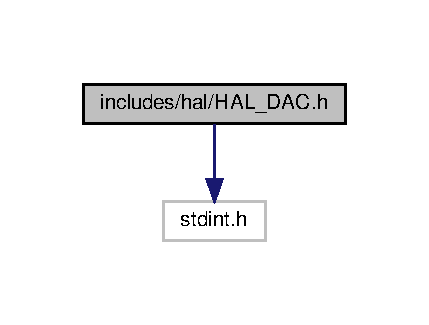
\includegraphics[width=206pt]{HAL__DAC_8h__incl}
\end{center}
\end{figure}
\subsection*{Estructuras de datos}
\begin{DoxyCompactItemize}
\item 
struct \hyperlink{HAL__DAC_8h_structhal__dac__ctrl__config__t}{hal\+\_\+dac\+\_\+ctrl\+\_\+config\+\_\+t}
\end{DoxyCompactItemize}
\subsection*{Enumeraciones}
\begin{DoxyCompactItemize}
\item 
\mbox{\Hypertarget{HAL__DAC_8h_a36a28cc0fff9972f139b7b4959f691e9}\label{HAL__DAC_8h_a36a28cc0fff9972f139b7b4959f691e9}} 
enum {\bfseries hal\+\_\+dac\+\_\+en} \{ {\bfseries H\+A\+L\+\_\+\+D\+A\+C\+\_\+0} = 0, 
{\bfseries H\+A\+L\+\_\+\+D\+A\+C\+\_\+1}
 \}
\item 
\mbox{\Hypertarget{HAL__DAC_8h_a060451e91c937afba2be341b4a8a78c6}\label{HAL__DAC_8h_a060451e91c937afba2be341b4a8a78c6}} 
enum {\bfseries hal\+\_\+dac\+\_\+settling\+\_\+time\+\_\+en} \{ {\bfseries H\+A\+L\+\_\+\+D\+A\+C\+\_\+\+S\+E\+T\+T\+L\+I\+N\+G\+\_\+\+T\+I\+M\+E\+\_\+1\+U\+S\+\_\+\+M\+AX} = 0, 
{\bfseries H\+A\+L\+\_\+\+D\+A\+C\+\_\+\+S\+E\+T\+T\+L\+I\+N\+G\+\_\+\+T\+I\+M\+E\+\_\+2\+\_\+5\+U\+S\+\_\+\+M\+AX}
 \}
\end{DoxyCompactItemize}
\subsection*{Funciones}
\begin{DoxyCompactItemize}
\item 
void \hyperlink{HAL__DAC_8h_a0c3bc10289bf53d637dcf325983d64b9}{hal\+\_\+dac\+\_\+init} (hal\+\_\+dac\+\_\+en dac, hal\+\_\+dac\+\_\+settling\+\_\+time\+\_\+en settling\+\_\+time, uint32\+\_\+t initial\+\_\+value)
\begin{DoxyCompactList}\small\item\em Inicializacion del D\+AC. \end{DoxyCompactList}\end{DoxyCompactItemize}


\subsection{Descripción detallada}
Declaraciones a nivel de aplicacion del periferico D\+AC (L\+P\+C845) 

\begin{DoxyAuthor}{Autor}
Augusto Santini 
\end{DoxyAuthor}
\begin{DoxyDate}{Fecha}
3/2020 
\end{DoxyDate}
\begin{DoxyVersion}{Versión}
1.\+0 
\end{DoxyVersion}


\subsection{Documentación de las estructuras de datos}
\index{hal\+\_\+dac\+\_\+ctrl\+\_\+config\+\_\+t@{hal\+\_\+dac\+\_\+ctrl\+\_\+config\+\_\+t}}\label{structhal__dac__ctrl__config__t}
\Hypertarget{HAL__DAC_8h_structhal__dac__ctrl__config__t}
\subsubsection{struct hal\+\_\+dac\+\_\+ctrl\+\_\+config\+\_\+t}
\begin{DoxyFields}{Campos de datos}
\mbox{\Hypertarget{HAL__DAC_8h_a3dfe52d3dda993a8648198e3957bbdcb}\label{HAL__DAC_8h_a3dfe52d3dda993a8648198e3957bbdcb}} 
uint8\_t&
count\_enable: 1&
\\
\hline

\mbox{\Hypertarget{HAL__DAC_8h_ace4cbb1d9df61bad809887daafeb3262}\label{HAL__DAC_8h_ace4cbb1d9df61bad809887daafeb3262}} 
uint8\_t&
double\_buffering: 1&
\\
\hline

\mbox{\Hypertarget{HAL__DAC_8h_a202a9cec987f30eea0427a8c08966d1f}\label{HAL__DAC_8h_a202a9cec987f30eea0427a8c08966d1f}} 
uint8\_t&
dma\_enable: 1&
\\
\hline

\mbox{\Hypertarget{HAL__DAC_8h_a674aba4c7104bedc212128ae5851d97f}\label{HAL__DAC_8h_a674aba4c7104bedc212128ae5851d97f}} 
uint8\_t&
dma\_request: 1&
\\
\hline

\end{DoxyFields}


\subsection{Documentación de las funciones}
\mbox{\Hypertarget{HAL__DAC_8h_a0c3bc10289bf53d637dcf325983d64b9}\label{HAL__DAC_8h_a0c3bc10289bf53d637dcf325983d64b9}} 
\index{H\+A\+L\+\_\+\+D\+A\+C.\+h@{H\+A\+L\+\_\+\+D\+A\+C.\+h}!hal\+\_\+dac\+\_\+init@{hal\+\_\+dac\+\_\+init}}
\index{hal\+\_\+dac\+\_\+init@{hal\+\_\+dac\+\_\+init}!H\+A\+L\+\_\+\+D\+A\+C.\+h@{H\+A\+L\+\_\+\+D\+A\+C.\+h}}
\subsubsection{\texorpdfstring{hal\+\_\+dac\+\_\+init()}{hal\_dac\_init()}}
{\footnotesize\ttfamily void hal\+\_\+dac\+\_\+init (\begin{DoxyParamCaption}\item[{hal\+\_\+dac\+\_\+en}]{dac,  }\item[{hal\+\_\+dac\+\_\+settling\+\_\+time\+\_\+en}]{settling\+\_\+time,  }\item[{uint32\+\_\+t}]{initial\+\_\+value }\end{DoxyParamCaption})}



Inicializacion del D\+AC. 


\begin{DoxyParams}[1]{Parámetros}
\mbox{\tt in}  & {\em dac} & Cual de los dos D\+A\+Cs inicializar \\
\hline
\mbox{\tt in}  & {\em settling\+\_\+time} & Velocidad de conversion del D\+AC \\
\hline
\mbox{\tt in}  & {\em initial\+\_\+value} & Valor inicial del D\+AC \\
\hline
\end{DoxyParams}

\hypertarget{HAL__GPIO_8h}{}\section{Referencia del Archivo includes/hal/\+H\+A\+L\+\_\+\+G\+P\+IO.h}
\label{HAL__GPIO_8h}\index{includes/hal/\+H\+A\+L\+\_\+\+G\+P\+I\+O.\+h@{includes/hal/\+H\+A\+L\+\_\+\+G\+P\+I\+O.\+h}}


Declaraciones a nivel de aplicacion del periferico G\+P\+IO (L\+P\+C845)  


{\ttfamily \#include $<$stdint.\+h$>$}\newline
Dependencia gráfica adjunta para H\+A\+L\+\_\+\+G\+P\+I\+O.\+h\+:\nopagebreak
\begin{figure}[H]
\begin{center}
\leavevmode
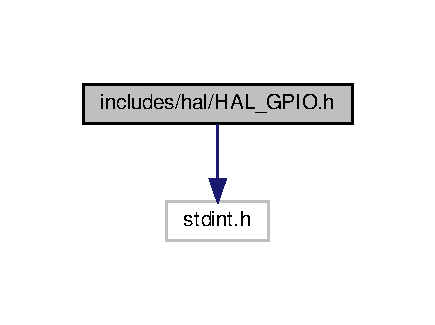
\includegraphics[width=209pt]{HAL__GPIO_8h__incl}
\end{center}
\end{figure}
Gráfico de los archivos que directa o indirectamente incluyen a este archivo\+:\nopagebreak
\begin{figure}[H]
\begin{center}
\leavevmode
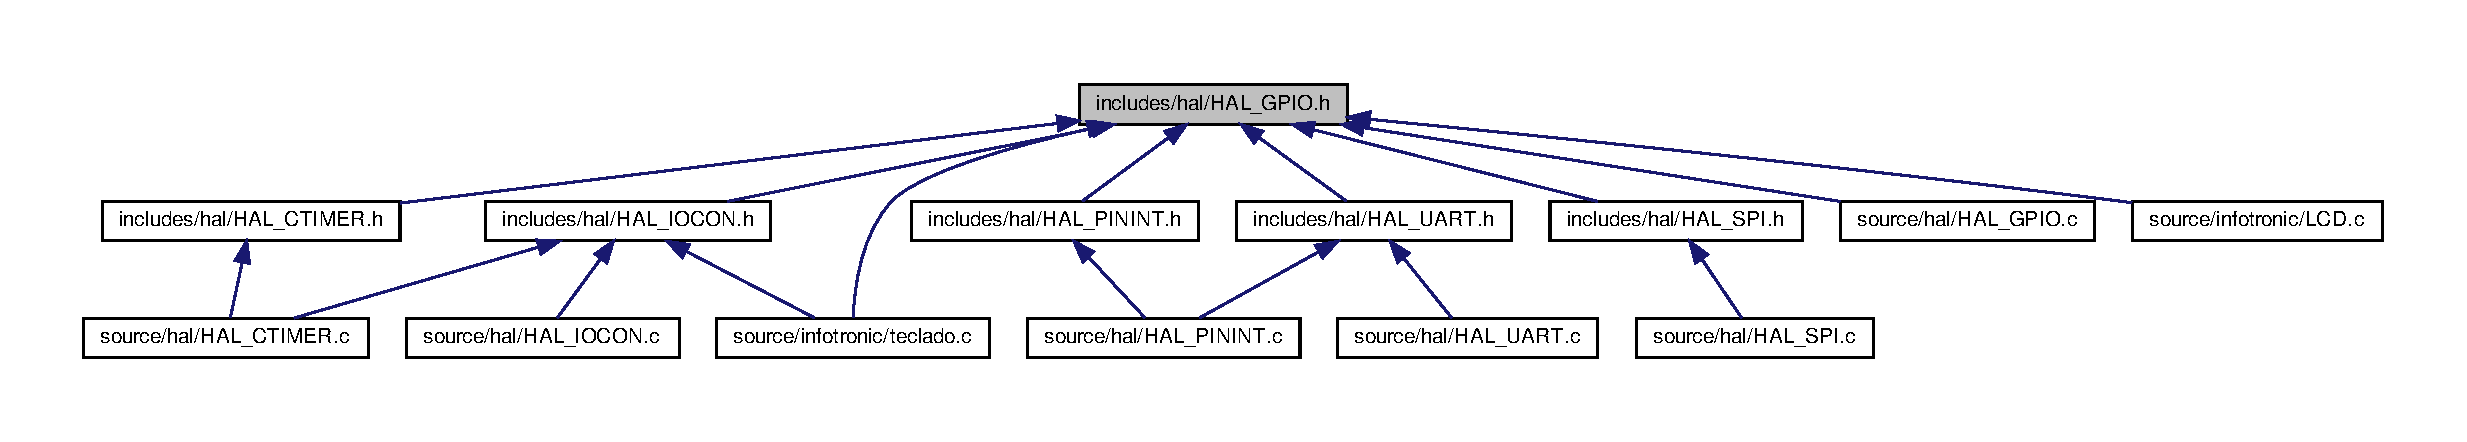
\includegraphics[width=350pt]{HAL__GPIO_8h__dep__incl}
\end{center}
\end{figure}
\subsection*{defines}
\begin{DoxyCompactItemize}
\item 
\mbox{\Hypertarget{HAL__GPIO_8h_ae0a26fe45351d3fab4b1bc5d59a6ea58}\label{HAL__GPIO_8h_ae0a26fe45351d3fab4b1bc5d59a6ea58}} 
\#define {\bfseries H\+A\+L\+\_\+\+G\+P\+I\+O\+\_\+\+P\+O\+R\+T\+P\+I\+N\+\_\+\+T\+O\+\_\+\+P\+O\+RT}(x)~(x / 32)
\item 
\mbox{\Hypertarget{HAL__GPIO_8h_a204f5d369f98d6f5fd068efb03ce09b8}\label{HAL__GPIO_8h_a204f5d369f98d6f5fd068efb03ce09b8}} 
\#define {\bfseries H\+A\+L\+\_\+\+G\+P\+I\+O\+\_\+\+P\+O\+R\+T\+P\+I\+N\+\_\+\+T\+O\+\_\+\+P\+IN}(x)~(x \% 32)
\end{DoxyCompactItemize}
\subsection*{Enumeraciones}
\begin{DoxyCompactItemize}
\item 
\mbox{\Hypertarget{HAL__GPIO_8h_a67db951437d45b48c1504058e8a48302}\label{HAL__GPIO_8h_a67db951437d45b48c1504058e8a48302}} 
enum {\bfseries hal\+\_\+gpio\+\_\+port\+\_\+en} \{ {\bfseries H\+A\+L\+\_\+\+G\+P\+I\+O\+\_\+\+P\+O\+R\+T\+\_\+0} = 0, 
{\bfseries H\+A\+L\+\_\+\+G\+P\+I\+O\+\_\+\+P\+O\+R\+T\+\_\+1}
 \}
\item 
\mbox{\Hypertarget{HAL__GPIO_8h_a5fd48fa8390fc0ec15d4d7f7c2bbc51b}\label{HAL__GPIO_8h_a5fd48fa8390fc0ec15d4d7f7c2bbc51b}} 
enum {\bfseries hal\+\_\+gpio\+\_\+portpin\+\_\+en} \{ \newline
{\bfseries H\+A\+L\+\_\+\+G\+P\+I\+O\+\_\+\+P\+O\+R\+T\+P\+I\+N\+\_\+0\+\_\+0} = 0, 
{\bfseries H\+A\+L\+\_\+\+G\+P\+I\+O\+\_\+\+P\+O\+R\+T\+P\+I\+N\+\_\+0\+\_\+1}, 
{\bfseries H\+A\+L\+\_\+\+G\+P\+I\+O\+\_\+\+P\+O\+R\+T\+P\+I\+N\+\_\+0\+\_\+2}, 
{\bfseries H\+A\+L\+\_\+\+G\+P\+I\+O\+\_\+\+P\+O\+R\+T\+P\+I\+N\+\_\+0\+\_\+3}, 
\newline
{\bfseries H\+A\+L\+\_\+\+G\+P\+I\+O\+\_\+\+P\+O\+R\+T\+P\+I\+N\+\_\+0\+\_\+4}, 
{\bfseries H\+A\+L\+\_\+\+G\+P\+I\+O\+\_\+\+P\+O\+R\+T\+P\+I\+N\+\_\+0\+\_\+5}, 
{\bfseries H\+A\+L\+\_\+\+G\+P\+I\+O\+\_\+\+P\+O\+R\+T\+P\+I\+N\+\_\+0\+\_\+6}, 
{\bfseries H\+A\+L\+\_\+\+G\+P\+I\+O\+\_\+\+P\+O\+R\+T\+P\+I\+N\+\_\+0\+\_\+7}, 
\newline
{\bfseries H\+A\+L\+\_\+\+G\+P\+I\+O\+\_\+\+P\+O\+R\+T\+P\+I\+N\+\_\+0\+\_\+8}, 
{\bfseries H\+A\+L\+\_\+\+G\+P\+I\+O\+\_\+\+P\+O\+R\+T\+P\+I\+N\+\_\+0\+\_\+9}, 
{\bfseries H\+A\+L\+\_\+\+G\+P\+I\+O\+\_\+\+P\+O\+R\+T\+P\+I\+N\+\_\+0\+\_\+10}, 
{\bfseries H\+A\+L\+\_\+\+G\+P\+I\+O\+\_\+\+P\+O\+R\+T\+P\+I\+N\+\_\+0\+\_\+11}, 
\newline
{\bfseries H\+A\+L\+\_\+\+G\+P\+I\+O\+\_\+\+P\+O\+R\+T\+P\+I\+N\+\_\+0\+\_\+12}, 
{\bfseries H\+A\+L\+\_\+\+G\+P\+I\+O\+\_\+\+P\+O\+R\+T\+P\+I\+N\+\_\+0\+\_\+13}, 
{\bfseries H\+A\+L\+\_\+\+G\+P\+I\+O\+\_\+\+P\+O\+R\+T\+P\+I\+N\+\_\+0\+\_\+14}, 
{\bfseries H\+A\+L\+\_\+\+G\+P\+I\+O\+\_\+\+P\+O\+R\+T\+P\+I\+N\+\_\+0\+\_\+15}, 
\newline
{\bfseries H\+A\+L\+\_\+\+G\+P\+I\+O\+\_\+\+P\+O\+R\+T\+P\+I\+N\+\_\+0\+\_\+16}, 
{\bfseries H\+A\+L\+\_\+\+G\+P\+I\+O\+\_\+\+P\+O\+R\+T\+P\+I\+N\+\_\+0\+\_\+17}, 
{\bfseries H\+A\+L\+\_\+\+G\+P\+I\+O\+\_\+\+P\+O\+R\+T\+P\+I\+N\+\_\+0\+\_\+18}, 
{\bfseries H\+A\+L\+\_\+\+G\+P\+I\+O\+\_\+\+P\+O\+R\+T\+P\+I\+N\+\_\+0\+\_\+19}, 
\newline
{\bfseries H\+A\+L\+\_\+\+G\+P\+I\+O\+\_\+\+P\+O\+R\+T\+P\+I\+N\+\_\+0\+\_\+20}, 
{\bfseries H\+A\+L\+\_\+\+G\+P\+I\+O\+\_\+\+P\+O\+R\+T\+P\+I\+N\+\_\+0\+\_\+21}, 
{\bfseries H\+A\+L\+\_\+\+G\+P\+I\+O\+\_\+\+P\+O\+R\+T\+P\+I\+N\+\_\+0\+\_\+22}, 
{\bfseries H\+A\+L\+\_\+\+G\+P\+I\+O\+\_\+\+P\+O\+R\+T\+P\+I\+N\+\_\+0\+\_\+23}, 
\newline
{\bfseries H\+A\+L\+\_\+\+G\+P\+I\+O\+\_\+\+P\+O\+R\+T\+P\+I\+N\+\_\+0\+\_\+24}, 
{\bfseries H\+A\+L\+\_\+\+G\+P\+I\+O\+\_\+\+P\+O\+R\+T\+P\+I\+N\+\_\+0\+\_\+25}, 
{\bfseries H\+A\+L\+\_\+\+G\+P\+I\+O\+\_\+\+P\+O\+R\+T\+P\+I\+N\+\_\+0\+\_\+26}, 
{\bfseries H\+A\+L\+\_\+\+G\+P\+I\+O\+\_\+\+P\+O\+R\+T\+P\+I\+N\+\_\+0\+\_\+27}, 
\newline
{\bfseries H\+A\+L\+\_\+\+G\+P\+I\+O\+\_\+\+P\+O\+R\+T\+P\+I\+N\+\_\+0\+\_\+28}, 
{\bfseries H\+A\+L\+\_\+\+G\+P\+I\+O\+\_\+\+P\+O\+R\+T\+P\+I\+N\+\_\+0\+\_\+29}, 
{\bfseries H\+A\+L\+\_\+\+G\+P\+I\+O\+\_\+\+P\+O\+R\+T\+P\+I\+N\+\_\+0\+\_\+30}, 
{\bfseries H\+A\+L\+\_\+\+G\+P\+I\+O\+\_\+\+P\+O\+R\+T\+P\+I\+N\+\_\+0\+\_\+31}, 
\newline
{\bfseries H\+A\+L\+\_\+\+G\+P\+I\+O\+\_\+\+P\+O\+R\+T\+P\+I\+N\+\_\+1\+\_\+0}, 
{\bfseries H\+A\+L\+\_\+\+G\+P\+I\+O\+\_\+\+P\+O\+R\+T\+P\+I\+N\+\_\+1\+\_\+1}, 
{\bfseries H\+A\+L\+\_\+\+G\+P\+I\+O\+\_\+\+P\+O\+R\+T\+P\+I\+N\+\_\+1\+\_\+2}, 
{\bfseries H\+A\+L\+\_\+\+G\+P\+I\+O\+\_\+\+P\+O\+R\+T\+P\+I\+N\+\_\+1\+\_\+3}, 
\newline
{\bfseries H\+A\+L\+\_\+\+G\+P\+I\+O\+\_\+\+P\+O\+R\+T\+P\+I\+N\+\_\+1\+\_\+4}, 
{\bfseries H\+A\+L\+\_\+\+G\+P\+I\+O\+\_\+\+P\+O\+R\+T\+P\+I\+N\+\_\+1\+\_\+5}, 
{\bfseries H\+A\+L\+\_\+\+G\+P\+I\+O\+\_\+\+P\+O\+R\+T\+P\+I\+N\+\_\+1\+\_\+6}, 
{\bfseries H\+A\+L\+\_\+\+G\+P\+I\+O\+\_\+\+P\+O\+R\+T\+P\+I\+N\+\_\+1\+\_\+7}, 
\newline
{\bfseries H\+A\+L\+\_\+\+G\+P\+I\+O\+\_\+\+P\+O\+R\+T\+P\+I\+N\+\_\+1\+\_\+8}, 
{\bfseries H\+A\+L\+\_\+\+G\+P\+I\+O\+\_\+\+P\+O\+R\+T\+P\+I\+N\+\_\+1\+\_\+9}, 
{\bfseries H\+A\+L\+\_\+\+G\+P\+I\+O\+\_\+\+P\+O\+R\+T\+P\+I\+N\+\_\+\+N\+O\+T\+\_\+\+U\+S\+ED}
 \}
\item 
\mbox{\Hypertarget{HAL__GPIO_8h_acdde9afffdc2043850035540298a5473}\label{HAL__GPIO_8h_acdde9afffdc2043850035540298a5473}} 
enum {\bfseries hal\+\_\+gpio\+\_\+dir\+\_\+en} \{ {\bfseries H\+A\+L\+\_\+\+G\+P\+I\+O\+\_\+\+D\+I\+R\+\_\+\+I\+N\+P\+UT} = 0, 
{\bfseries H\+A\+L\+\_\+\+G\+P\+I\+O\+\_\+\+D\+I\+R\+\_\+\+O\+U\+T\+P\+UT}
 \}
\end{DoxyCompactItemize}
\subsection*{Funciones}
\begin{DoxyCompactItemize}
\item 
void \hyperlink{HAL__GPIO_8h_a315deab93915cc375acef1e81046f2bc}{hal\+\_\+gpio\+\_\+init} (hal\+\_\+gpio\+\_\+port\+\_\+en port)
\begin{DoxyCompactList}\small\item\em Inicializar un puerto. \end{DoxyCompactList}\item 
void \hyperlink{HAL__GPIO_8h_a88843594aedf65f8f0c97eade8853124}{hal\+\_\+gpio\+\_\+set\+\_\+dir} (hal\+\_\+gpio\+\_\+portpin\+\_\+en portpin, hal\+\_\+gpio\+\_\+dir\+\_\+en dir, uint8\+\_\+t initial\+\_\+state)
\begin{DoxyCompactList}\small\item\em Fijar direccion de una G\+P\+IO. \end{DoxyCompactList}\item 
void \hyperlink{HAL__GPIO_8h_abb1f2e1042b1fe64677f95a439076527}{hal\+\_\+gpio\+\_\+set\+\_\+pin} (hal\+\_\+gpio\+\_\+portpin\+\_\+en portpin)
\begin{DoxyCompactList}\small\item\em Fijar estado activo de una G\+P\+IO. \end{DoxyCompactList}\item 
void \hyperlink{HAL__GPIO_8h_acdea7b3a5bae213e58bce78fb5356eb2}{hal\+\_\+gpio\+\_\+clear\+\_\+pin} (hal\+\_\+gpio\+\_\+portpin\+\_\+en portpin)
\begin{DoxyCompactList}\small\item\em Fijar estado inactivo de una G\+P\+IO. \end{DoxyCompactList}\item 
void \hyperlink{HAL__GPIO_8h_a3c6ea73afbcc76405ef5c6ac22bc57ac}{hal\+\_\+gpio\+\_\+toggle\+\_\+pin} (hal\+\_\+gpio\+\_\+portpin\+\_\+en portpin)
\begin{DoxyCompactList}\small\item\em Invertir estado de una G\+P\+IO. \end{DoxyCompactList}\item 
uint8\+\_\+t \hyperlink{HAL__GPIO_8h_a84780bdc959ae4cc21cdc2fd063a1ed6}{hal\+\_\+gpio\+\_\+read\+\_\+pin} (hal\+\_\+gpio\+\_\+portpin\+\_\+en portpin)
\begin{DoxyCompactList}\small\item\em Leer el estado de una G\+P\+IO. \end{DoxyCompactList}\end{DoxyCompactItemize}


\subsection{Descripción detallada}
Declaraciones a nivel de aplicacion del periferico G\+P\+IO (L\+P\+C845) 

\begin{DoxyAuthor}{Autor}
Augusto Santini 
\end{DoxyAuthor}
\begin{DoxyDate}{Fecha}
3/2020 
\end{DoxyDate}
\begin{DoxyVersion}{Versión}
1.\+0 
\end{DoxyVersion}


\subsection{Documentación de las funciones}
\mbox{\Hypertarget{HAL__GPIO_8h_a315deab93915cc375acef1e81046f2bc}\label{HAL__GPIO_8h_a315deab93915cc375acef1e81046f2bc}} 
\index{H\+A\+L\+\_\+\+G\+P\+I\+O.\+h@{H\+A\+L\+\_\+\+G\+P\+I\+O.\+h}!hal\+\_\+gpio\+\_\+init@{hal\+\_\+gpio\+\_\+init}}
\index{hal\+\_\+gpio\+\_\+init@{hal\+\_\+gpio\+\_\+init}!H\+A\+L\+\_\+\+G\+P\+I\+O.\+h@{H\+A\+L\+\_\+\+G\+P\+I\+O.\+h}}
\subsubsection{\texorpdfstring{hal\+\_\+gpio\+\_\+init()}{hal\_gpio\_init()}}
{\footnotesize\ttfamily void hal\+\_\+gpio\+\_\+init (\begin{DoxyParamCaption}\item[{hal\+\_\+gpio\+\_\+port\+\_\+en}]{port }\end{DoxyParamCaption})}



Inicializar un puerto. 


\begin{DoxyParams}[1]{Parámetros}
\mbox{\tt in}  & {\em port} & Puerto a inicializar \\
\hline
\end{DoxyParams}
\mbox{\Hypertarget{HAL__GPIO_8h_a88843594aedf65f8f0c97eade8853124}\label{HAL__GPIO_8h_a88843594aedf65f8f0c97eade8853124}} 
\index{H\+A\+L\+\_\+\+G\+P\+I\+O.\+h@{H\+A\+L\+\_\+\+G\+P\+I\+O.\+h}!hal\+\_\+gpio\+\_\+set\+\_\+dir@{hal\+\_\+gpio\+\_\+set\+\_\+dir}}
\index{hal\+\_\+gpio\+\_\+set\+\_\+dir@{hal\+\_\+gpio\+\_\+set\+\_\+dir}!H\+A\+L\+\_\+\+G\+P\+I\+O.\+h@{H\+A\+L\+\_\+\+G\+P\+I\+O.\+h}}
\subsubsection{\texorpdfstring{hal\+\_\+gpio\+\_\+set\+\_\+dir()}{hal\_gpio\_set\_dir()}}
{\footnotesize\ttfamily void hal\+\_\+gpio\+\_\+set\+\_\+dir (\begin{DoxyParamCaption}\item[{hal\+\_\+gpio\+\_\+portpin\+\_\+en}]{portpin,  }\item[{hal\+\_\+gpio\+\_\+dir\+\_\+en}]{dir,  }\item[{uint8\+\_\+t}]{initial\+\_\+state }\end{DoxyParamCaption})}



Fijar direccion de una G\+P\+IO. 


\begin{DoxyParams}[1]{Parámetros}
\mbox{\tt in}  & {\em portpin} & Numero de puerto/pin a configurar \\
\hline
\mbox{\tt in}  & {\em dir} & Direccion deseada \\
\hline
\mbox{\tt in}  & {\em initial\+\_\+state} & Estado inicial (aplica para salidas nada mas) \\
\hline
\end{DoxyParams}
\mbox{\Hypertarget{HAL__GPIO_8h_abb1f2e1042b1fe64677f95a439076527}\label{HAL__GPIO_8h_abb1f2e1042b1fe64677f95a439076527}} 
\index{H\+A\+L\+\_\+\+G\+P\+I\+O.\+h@{H\+A\+L\+\_\+\+G\+P\+I\+O.\+h}!hal\+\_\+gpio\+\_\+set\+\_\+pin@{hal\+\_\+gpio\+\_\+set\+\_\+pin}}
\index{hal\+\_\+gpio\+\_\+set\+\_\+pin@{hal\+\_\+gpio\+\_\+set\+\_\+pin}!H\+A\+L\+\_\+\+G\+P\+I\+O.\+h@{H\+A\+L\+\_\+\+G\+P\+I\+O.\+h}}
\subsubsection{\texorpdfstring{hal\+\_\+gpio\+\_\+set\+\_\+pin()}{hal\_gpio\_set\_pin()}}
{\footnotesize\ttfamily void hal\+\_\+gpio\+\_\+set\+\_\+pin (\begin{DoxyParamCaption}\item[{hal\+\_\+gpio\+\_\+portpin\+\_\+en}]{portpin }\end{DoxyParamCaption})}



Fijar estado activo de una G\+P\+IO. 


\begin{DoxyParams}[1]{Parámetros}
\mbox{\tt in}  & {\em portpin} & Numero de puerto/pin a accionar \\
\hline
\end{DoxyParams}
\mbox{\Hypertarget{HAL__GPIO_8h_acdea7b3a5bae213e58bce78fb5356eb2}\label{HAL__GPIO_8h_acdea7b3a5bae213e58bce78fb5356eb2}} 
\index{H\+A\+L\+\_\+\+G\+P\+I\+O.\+h@{H\+A\+L\+\_\+\+G\+P\+I\+O.\+h}!hal\+\_\+gpio\+\_\+clear\+\_\+pin@{hal\+\_\+gpio\+\_\+clear\+\_\+pin}}
\index{hal\+\_\+gpio\+\_\+clear\+\_\+pin@{hal\+\_\+gpio\+\_\+clear\+\_\+pin}!H\+A\+L\+\_\+\+G\+P\+I\+O.\+h@{H\+A\+L\+\_\+\+G\+P\+I\+O.\+h}}
\subsubsection{\texorpdfstring{hal\+\_\+gpio\+\_\+clear\+\_\+pin()}{hal\_gpio\_clear\_pin()}}
{\footnotesize\ttfamily void hal\+\_\+gpio\+\_\+clear\+\_\+pin (\begin{DoxyParamCaption}\item[{hal\+\_\+gpio\+\_\+portpin\+\_\+en}]{portpin }\end{DoxyParamCaption})}



Fijar estado inactivo de una G\+P\+IO. 


\begin{DoxyParams}[1]{Parámetros}
\mbox{\tt in}  & {\em portpin} & Numero de puerto/pin a accionar \\
\hline
\end{DoxyParams}
\mbox{\Hypertarget{HAL__GPIO_8h_a3c6ea73afbcc76405ef5c6ac22bc57ac}\label{HAL__GPIO_8h_a3c6ea73afbcc76405ef5c6ac22bc57ac}} 
\index{H\+A\+L\+\_\+\+G\+P\+I\+O.\+h@{H\+A\+L\+\_\+\+G\+P\+I\+O.\+h}!hal\+\_\+gpio\+\_\+toggle\+\_\+pin@{hal\+\_\+gpio\+\_\+toggle\+\_\+pin}}
\index{hal\+\_\+gpio\+\_\+toggle\+\_\+pin@{hal\+\_\+gpio\+\_\+toggle\+\_\+pin}!H\+A\+L\+\_\+\+G\+P\+I\+O.\+h@{H\+A\+L\+\_\+\+G\+P\+I\+O.\+h}}
\subsubsection{\texorpdfstring{hal\+\_\+gpio\+\_\+toggle\+\_\+pin()}{hal\_gpio\_toggle\_pin()}}
{\footnotesize\ttfamily void hal\+\_\+gpio\+\_\+toggle\+\_\+pin (\begin{DoxyParamCaption}\item[{hal\+\_\+gpio\+\_\+portpin\+\_\+en}]{portpin }\end{DoxyParamCaption})}



Invertir estado de una G\+P\+IO. 


\begin{DoxyParams}[1]{Parámetros}
\mbox{\tt in}  & {\em portpin} & Numero de puerto/pin a accionar \\
\hline
\end{DoxyParams}
\mbox{\Hypertarget{HAL__GPIO_8h_a84780bdc959ae4cc21cdc2fd063a1ed6}\label{HAL__GPIO_8h_a84780bdc959ae4cc21cdc2fd063a1ed6}} 
\index{H\+A\+L\+\_\+\+G\+P\+I\+O.\+h@{H\+A\+L\+\_\+\+G\+P\+I\+O.\+h}!hal\+\_\+gpio\+\_\+read\+\_\+pin@{hal\+\_\+gpio\+\_\+read\+\_\+pin}}
\index{hal\+\_\+gpio\+\_\+read\+\_\+pin@{hal\+\_\+gpio\+\_\+read\+\_\+pin}!H\+A\+L\+\_\+\+G\+P\+I\+O.\+h@{H\+A\+L\+\_\+\+G\+P\+I\+O.\+h}}
\subsubsection{\texorpdfstring{hal\+\_\+gpio\+\_\+read\+\_\+pin()}{hal\_gpio\_read\_pin()}}
{\footnotesize\ttfamily uint8\+\_\+t hal\+\_\+gpio\+\_\+read\+\_\+pin (\begin{DoxyParamCaption}\item[{hal\+\_\+gpio\+\_\+portpin\+\_\+en}]{portpin }\end{DoxyParamCaption})}



Leer el estado de una G\+P\+IO. 


\begin{DoxyParams}[1]{Parámetros}
\mbox{\tt in}  & {\em portpin} & Numero de puerto/pin a accionar \\
\hline
\end{DoxyParams}
\begin{DoxyReturn}{Devuelve}
Estado actual de la G\+P\+IO 
\end{DoxyReturn}

\hypertarget{HAL__IOCON_8h}{}\section{Referencia del Archivo includes/hal/\+H\+A\+L\+\_\+\+I\+O\+C\+ON.h}
\label{HAL__IOCON_8h}\index{includes/hal/\+H\+A\+L\+\_\+\+I\+O\+C\+O\+N.\+h@{includes/hal/\+H\+A\+L\+\_\+\+I\+O\+C\+O\+N.\+h}}


Declaraciones a nivel de aplicacion del periferico I\+O\+C\+ON (L\+P\+C845)  


{\ttfamily \#include $<$H\+P\+L\+\_\+\+I\+O\+C\+O\+N.\+h$>$}\newline
{\ttfamily \#include $<$H\+A\+L\+\_\+\+G\+P\+I\+O.\+h$>$}\newline
Dependencia gráfica adjunta para H\+A\+L\+\_\+\+I\+O\+C\+O\+N.\+h\+:
\nopagebreak
\begin{figure}[H]
\begin{center}
\leavevmode
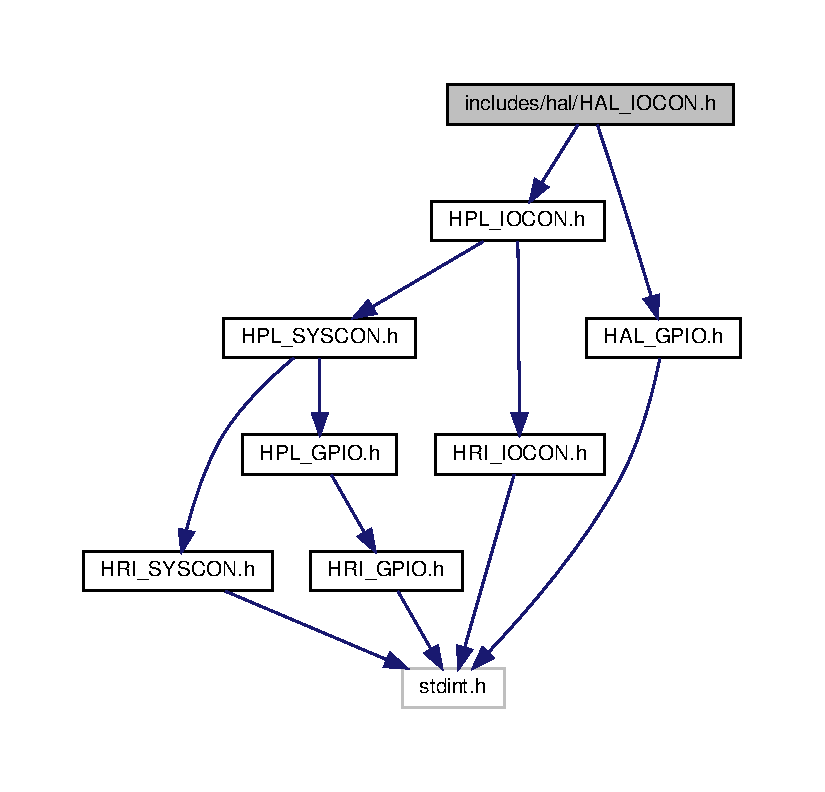
\includegraphics[width=350pt]{d2/ddf/HAL__IOCON_8h__incl}
\end{center}
\end{figure}
Gráfico de los archivos que directa o indirectamente incluyen a este archivo\+:\nopagebreak
\begin{figure}[H]
\begin{center}
\leavevmode
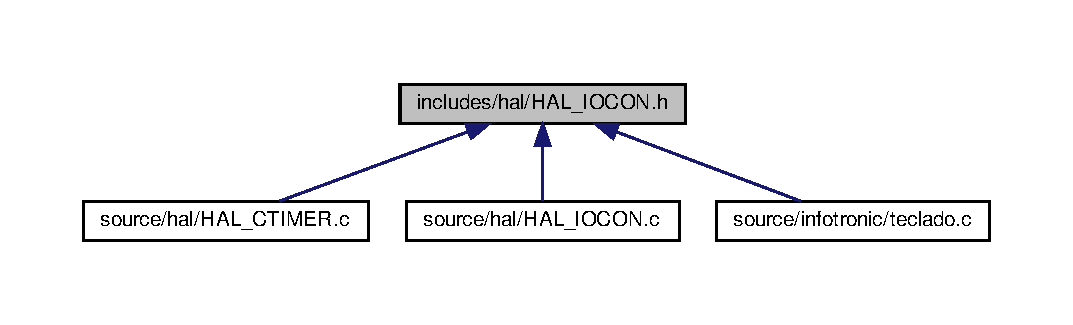
\includegraphics[width=350pt]{d7/de0/HAL__IOCON_8h__dep__incl}
\end{center}
\end{figure}
\subsection*{Estructuras de datos}
\begin{DoxyCompactItemize}
\item 
struct \hyperlink{HAL__IOCON_8h_dc/df0/structhal__iocon__config__t}{hal\+\_\+iocon\+\_\+config\+\_\+t}
\end{DoxyCompactItemize}
\subsection*{Enumeraciones}
\begin{DoxyCompactItemize}
\item 
\mbox{\Hypertarget{HAL__IOCON_8h_a63ecccb192eecfde5513839ac2a69431}\label{HAL__IOCON_8h_a63ecccb192eecfde5513839ac2a69431}} 
enum {\bfseries hal\+\_\+iocon\+\_\+pull\+\_\+mode\+\_\+en} \{ {\bfseries H\+A\+L\+\_\+\+I\+O\+C\+O\+N\+\_\+\+P\+U\+L\+L\+\_\+\+N\+O\+NE} = 0, 
{\bfseries H\+A\+L\+\_\+\+I\+O\+C\+O\+N\+\_\+\+P\+U\+L\+L\+\_\+\+D\+O\+WN}, 
{\bfseries H\+A\+L\+\_\+\+I\+O\+C\+O\+N\+\_\+\+P\+U\+L\+L\+\_\+\+UP}, 
{\bfseries H\+A\+L\+\_\+\+I\+O\+C\+O\+N\+\_\+\+P\+U\+L\+L\+\_\+\+R\+E\+P\+E\+A\+T\+ER}
 \}
\item 
\mbox{\Hypertarget{HAL__IOCON_8h_a41306d2caced0b5f04e58a44d48dfd09}\label{HAL__IOCON_8h_a41306d2caced0b5f04e58a44d48dfd09}} 
enum {\bfseries hal\+\_\+iocon\+\_\+sample\+\_\+mode\+\_\+en} \{ {\bfseries H\+A\+L\+\_\+\+I\+O\+C\+O\+N\+\_\+\+S\+A\+M\+P\+L\+E\+\_\+\+M\+O\+D\+E\+\_\+\+B\+Y\+P\+A\+SS} = 0, 
{\bfseries H\+A\+L\+\_\+\+I\+O\+C\+O\+N\+\_\+\+S\+A\+M\+P\+L\+E\+\_\+\+M\+O\+D\+E\+\_\+1\+\_\+\+C\+L\+O\+CK}, 
{\bfseries H\+A\+L\+\_\+\+I\+O\+C\+O\+N\+\_\+\+S\+A\+M\+P\+L\+E\+\_\+\+M\+O\+D\+E\+\_\+2\+\_\+\+C\+L\+O\+CK}, 
{\bfseries H\+A\+L\+\_\+\+I\+O\+C\+O\+N\+\_\+\+S\+A\+M\+P\+L\+E\+\_\+\+M\+O\+D\+E\+\_\+3\+\_\+\+C\+L\+O\+CK}
 \}
\item 
\mbox{\Hypertarget{HAL__IOCON_8h_a0b6a60b068de7a0cb787eaa62055acae}\label{HAL__IOCON_8h_a0b6a60b068de7a0cb787eaa62055acae}} 
enum {\bfseries hal\+\_\+iocon\+\_\+clk\+\_\+sel\+\_\+en} \{ \newline
{\bfseries H\+A\+L\+\_\+\+I\+O\+C\+O\+N\+\_\+\+C\+L\+K\+\_\+\+D\+I\+V\+\_\+0} = 0, 
{\bfseries H\+A\+L\+\_\+\+I\+O\+C\+O\+N\+\_\+\+C\+L\+K\+\_\+\+D\+I\+V\+\_\+1}, 
{\bfseries H\+A\+L\+\_\+\+I\+O\+C\+O\+N\+\_\+\+C\+L\+K\+\_\+\+D\+I\+V\+\_\+2}, 
{\bfseries H\+A\+L\+\_\+\+I\+O\+C\+O\+N\+\_\+\+C\+L\+K\+\_\+\+D\+I\+V\+\_\+3}, 
\newline
{\bfseries H\+A\+L\+\_\+\+I\+O\+C\+O\+N\+\_\+\+C\+L\+K\+\_\+\+D\+I\+V\+\_\+4}, 
{\bfseries H\+A\+L\+\_\+\+I\+O\+C\+O\+N\+\_\+\+C\+L\+K\+\_\+\+D\+I\+V\+\_\+5}, 
{\bfseries H\+A\+L\+\_\+\+I\+O\+C\+O\+N\+\_\+\+C\+L\+K\+\_\+\+D\+I\+V\+\_\+6}
 \}
\item 
\mbox{\Hypertarget{HAL__IOCON_8h_ac5adeae1bf96c489da06d9447800e9c0}\label{HAL__IOCON_8h_ac5adeae1bf96c489da06d9447800e9c0}} 
enum {\bfseries hal\+\_\+iocon\+\_\+iic\+\_\+mode\+\_\+en} \{ {\bfseries H\+A\+L\+\_\+\+I\+O\+C\+O\+N\+\_\+\+I\+I\+C\+\_\+\+M\+O\+D\+E\+\_\+\+S\+T\+A\+N\+D\+A\+RD} = 0, 
{\bfseries H\+A\+L\+\_\+\+I\+O\+C\+O\+N\+\_\+\+I\+I\+C\+\_\+\+M\+O\+D\+E\+\_\+\+G\+P\+IO}, 
{\bfseries H\+A\+L\+\_\+\+I\+O\+C\+O\+N\+\_\+\+I\+I\+C\+\_\+\+M\+O\+D\+E\+\_\+\+F\+A\+S\+T\+\_\+\+M\+O\+DE}
 \}
\end{DoxyCompactItemize}
\subsection*{Funciones}
\begin{DoxyCompactItemize}
\item 
void \hyperlink{HAL__IOCON_8h_af7f22380a268cadbc2928e6a5bb18b88}{hal\+\_\+iocon\+\_\+config\+\_\+io} (hal\+\_\+gpio\+\_\+portpin\+\_\+en portpin, const \hyperlink{HAL__IOCON_8h_dc/df0/structhal__iocon__config__t}{hal\+\_\+iocon\+\_\+config\+\_\+t} $\ast$config)
\begin{DoxyCompactList}\small\item\em Configuracion de un pin. \end{DoxyCompactList}\end{DoxyCompactItemize}


\subsection{Descripción detallada}
Declaraciones a nivel de aplicacion del periferico I\+O\+C\+ON (L\+P\+C845) 

\begin{DoxyAuthor}{Autor}
Augusto Santini 
\end{DoxyAuthor}
\begin{DoxyDate}{Fecha}
3/2020 
\end{DoxyDate}
\begin{DoxyVersion}{Versión}
1.\+0 
\end{DoxyVersion}


\subsection{Documentación de las estructuras de datos}
\index{hal\+\_\+iocon\+\_\+config\+\_\+t@{hal\+\_\+iocon\+\_\+config\+\_\+t}}\label{structhal__iocon__config__t}
\Hypertarget{HAL__IOCON_8h_structhal__iocon__config__t}
\subsubsection{struct hal\+\_\+iocon\+\_\+config\+\_\+t}
\begin{DoxyFields}{Campos de datos}
\mbox{\Hypertarget{HAL__IOCON_8h_aa22f2560bc78d947824f4cfe5124eda7}\label{HAL__IOCON_8h_aa22f2560bc78d947824f4cfe5124eda7}} 
hal\_iocon\_pull\_mode\_en&
pull\_mode&
\\
\hline

\mbox{\Hypertarget{HAL__IOCON_8h_a2e9773d4803e8e976a13292cd2ad0c7a}\label{HAL__IOCON_8h_a2e9773d4803e8e976a13292cd2ad0c7a}} 
uint8\_t&
hysteresis&
\\
\hline

\mbox{\Hypertarget{HAL__IOCON_8h_a72cc41e5bf068e3e77e04797ad0927da}\label{HAL__IOCON_8h_a72cc41e5bf068e3e77e04797ad0927da}} 
uint8\_t&
invert\_input&
\\
\hline

\mbox{\Hypertarget{HAL__IOCON_8h_a1e960a1499ff856953454bb4bae0cb79}\label{HAL__IOCON_8h_a1e960a1499ff856953454bb4bae0cb79}} 
uint8\_t&
open\_drain&
\\
\hline

\mbox{\Hypertarget{HAL__IOCON_8h_a2bd76ef14f9b9048b414adbcd623d390}\label{HAL__IOCON_8h_a2bd76ef14f9b9048b414adbcd623d390}} 
hal\_iocon\_sample\_mode\_en&
sample\_mode&
\\
\hline

\mbox{\Hypertarget{HAL__IOCON_8h_a088a30034e6d3ce3ae44f171eebf8679}\label{HAL__IOCON_8h_a088a30034e6d3ce3ae44f171eebf8679}} 
hal\_iocon\_clk\_sel\_en&
clk\_sel&
\\
\hline

\mbox{\Hypertarget{HAL__IOCON_8h_a9444f75dcd09dd998209e13f4df83b11}\label{HAL__IOCON_8h_a9444f75dcd09dd998209e13f4df83b11}} 
uint8\_t&
dac\_mode&
\\
\hline

\mbox{\Hypertarget{HAL__IOCON_8h_ab637420afee560be573a20f19fbb0e1a}\label{HAL__IOCON_8h_ab637420afee560be573a20f19fbb0e1a}} 
hal\_iocon\_iic\_mode\_en&
iic\_mode&
\\
\hline

\end{DoxyFields}


\subsection{Documentación de las funciones}
\mbox{\Hypertarget{HAL__IOCON_8h_af7f22380a268cadbc2928e6a5bb18b88}\label{HAL__IOCON_8h_af7f22380a268cadbc2928e6a5bb18b88}} 
\index{H\+A\+L\+\_\+\+I\+O\+C\+O\+N.\+h@{H\+A\+L\+\_\+\+I\+O\+C\+O\+N.\+h}!hal\+\_\+iocon\+\_\+config\+\_\+io@{hal\+\_\+iocon\+\_\+config\+\_\+io}}
\index{hal\+\_\+iocon\+\_\+config\+\_\+io@{hal\+\_\+iocon\+\_\+config\+\_\+io}!H\+A\+L\+\_\+\+I\+O\+C\+O\+N.\+h@{H\+A\+L\+\_\+\+I\+O\+C\+O\+N.\+h}}
\subsubsection{\texorpdfstring{hal\+\_\+iocon\+\_\+config\+\_\+io()}{hal\_iocon\_config\_io()}}
{\footnotesize\ttfamily void hal\+\_\+iocon\+\_\+config\+\_\+io (\begin{DoxyParamCaption}\item[{hal\+\_\+gpio\+\_\+portpin\+\_\+en}]{portpin,  }\item[{const \hyperlink{HAL__IOCON_8h_dc/df0/structhal__iocon__config__t}{hal\+\_\+iocon\+\_\+config\+\_\+t} $\ast$}]{config }\end{DoxyParamCaption})}



Configuracion de un pin. 


\begin{DoxyParams}[1]{Parámetros}
\mbox{\tt in}  & {\em portpin} & Puerto/pin a configurar \\
\hline
\mbox{\tt in}  & {\em pin\+\_\+config} & Puntero a estructura de configuracion del pin \\
\hline
\end{DoxyParams}

\hypertarget{HAL__PININT_8h}{}\doxysection{Referencia del Archivo includes/hal/\+H\+A\+L\+\_\+\+P\+I\+N\+I\+NT.h}
\label{HAL__PININT_8h}\index{includes/hal/HAL\_PININT.h@{includes/hal/HAL\_PININT.h}}


Declaraciones a nivel de aplicacion del periferico P\+I\+N\+I\+NT (L\+P\+C845)  


{\ttfamily \#include $<$stdint.\+h$>$}\newline
{\ttfamily \#include $<$H\+A\+L\+\_\+\+G\+P\+I\+O.\+h$>$}\newline
Dependencia gráfica adjunta para H\+A\+L\+\_\+\+P\+I\+N\+I\+N\+T.\+h\+:\nopagebreak
\begin{figure}[H]
\begin{center}
\leavevmode
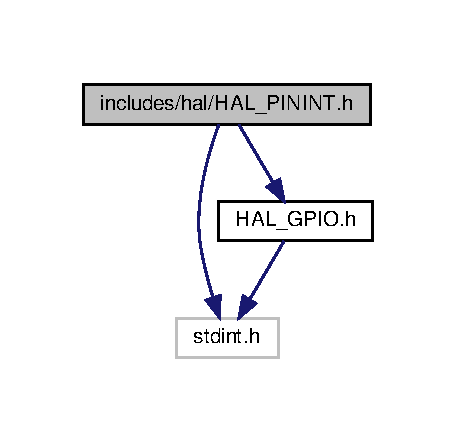
\includegraphics[width=219pt]{HAL__PININT_8h__incl}
\end{center}
\end{figure}
\doxysubsection*{Estructuras de datos}
\begin{DoxyCompactItemize}
\item 
struct \mbox{\hyperlink{structhal__pinint__config__t}{hal\+\_\+pinint\+\_\+config\+\_\+t}}
\end{DoxyCompactItemize}
\doxysubsection*{Enumeraciones}
\begin{DoxyCompactItemize}
\item 
\mbox{\Hypertarget{HAL__PININT_8h_a4ae16eed9cc4c0afbb4b43d8ff47c87c}\label{HAL__PININT_8h_a4ae16eed9cc4c0afbb4b43d8ff47c87c}} 
enum {\bfseries hal\+\_\+pinint\+\_\+channel\+\_\+en} \{ \newline
{\bfseries H\+A\+L\+\_\+\+P\+I\+N\+I\+N\+T\+\_\+\+C\+H\+A\+N\+N\+E\+L\+\_\+0} = 0, 
{\bfseries H\+A\+L\+\_\+\+P\+I\+N\+I\+N\+T\+\_\+\+C\+H\+A\+N\+N\+E\+L\+\_\+1}, 
{\bfseries H\+A\+L\+\_\+\+P\+I\+N\+I\+N\+T\+\_\+\+C\+H\+A\+N\+N\+E\+L\+\_\+2}, 
{\bfseries H\+A\+L\+\_\+\+P\+I\+N\+I\+N\+T\+\_\+\+C\+H\+A\+N\+N\+E\+L\+\_\+3}, 
\newline
{\bfseries H\+A\+L\+\_\+\+P\+I\+N\+I\+N\+T\+\_\+\+C\+H\+A\+N\+N\+E\+L\+\_\+4}, 
{\bfseries H\+A\+L\+\_\+\+P\+I\+N\+I\+N\+T\+\_\+\+C\+H\+A\+N\+N\+E\+L\+\_\+5}, 
{\bfseries H\+A\+L\+\_\+\+P\+I\+N\+I\+N\+T\+\_\+\+C\+H\+A\+N\+N\+E\+L\+\_\+6}, 
{\bfseries H\+A\+L\+\_\+\+P\+I\+N\+I\+N\+T\+\_\+\+C\+H\+A\+N\+N\+E\+L\+\_\+7}
 \}
\item 
\mbox{\Hypertarget{HAL__PININT_8h_a5a9a36a223fb9ec5c125d0acdc1c8ba3}\label{HAL__PININT_8h_a5a9a36a223fb9ec5c125d0acdc1c8ba3}} 
enum {\bfseries hal\+\_\+pinint\+\_\+interrupt\+\_\+mode\+\_\+en} \{ {\bfseries H\+A\+L\+\_\+\+P\+I\+N\+I\+N\+T\+\_\+\+I\+N\+T\+E\+R\+R\+U\+P\+T\+\_\+\+M\+O\+D\+E\+\_\+\+E\+D\+GE} = 0, 
{\bfseries H\+A\+L\+\_\+\+P\+I\+N\+I\+N\+T\+\_\+\+I\+N\+T\+E\+R\+R\+U\+P\+T\+\_\+\+M\+O\+D\+E\+\_\+\+L\+E\+V\+EL}
 \}
\item 
\mbox{\Hypertarget{HAL__PININT_8h_af9e709e533d1b2848c2b7a56c70e6bcb}\label{HAL__PININT_8h_af9e709e533d1b2848c2b7a56c70e6bcb}} 
enum {\bfseries hal\+\_\+pinint\+\_\+level\+\_\+int\+\_\+en} \{ {\bfseries H\+A\+L\+\_\+\+P\+I\+N\+I\+N\+T\+\_\+\+L\+E\+V\+E\+L\+\_\+\+I\+N\+T\+\_\+\+H\+I\+GH} = 0, 
{\bfseries H\+A\+L\+\_\+\+P\+I\+N\+I\+N\+T\+\_\+\+L\+E\+V\+E\+L\+\_\+\+I\+N\+T\+\_\+\+L\+OW}
 \}
\end{DoxyCompactItemize}
\doxysubsection*{Funciones}
\begin{DoxyCompactItemize}
\item 
\mbox{\Hypertarget{HAL__PININT_8h_aa0cbe5b8bc592e4731d28667e5dfc30f}\label{HAL__PININT_8h_aa0cbe5b8bc592e4731d28667e5dfc30f}} 
void \mbox{\hyperlink{HAL__PININT_8h_aa0cbe5b8bc592e4731d28667e5dfc30f}{hal\+\_\+pinint\+\_\+init}} (void)
\begin{DoxyCompactList}\small\item\em Inicializacion del modulo. \end{DoxyCompactList}\item 
void \mbox{\hyperlink{HAL__PININT_8h_a4b7e39b58f03c04edd28846ead64cbd7}{hal\+\_\+pinint\+\_\+configure\+\_\+pin\+\_\+interrupt}} (const \mbox{\hyperlink{structhal__pinint__config__t}{hal\+\_\+pinint\+\_\+config\+\_\+t}} $\ast$config)
\begin{DoxyCompactList}\small\item\em Configurar interrupciones de pin. \end{DoxyCompactList}\item 
void \mbox{\hyperlink{HAL__PININT_8h_a201dfb9bbe81b35792f5f335b9e7dc11}{hal\+\_\+pinint\+\_\+register\+\_\+callback}} (hal\+\_\+pinint\+\_\+channel\+\_\+en channel, void($\ast$new\+\_\+callback)(void))
\begin{DoxyCompactList}\small\item\em Registrar callback a llamar en interrupcion de P\+I\+N\+I\+N\+Tn. \end{DoxyCompactList}\end{DoxyCompactItemize}


\doxysubsection{Descripción detallada}
Declaraciones a nivel de aplicacion del periferico P\+I\+N\+I\+NT (L\+P\+C845) 

\begin{DoxyAuthor}{Autor}
Augusto Santini 
\end{DoxyAuthor}
\begin{DoxyDate}{Fecha}
3/2020 
\end{DoxyDate}
\begin{DoxyVersion}{Versión}
1.\+0 
\end{DoxyVersion}


\doxysubsection{Documentación de las funciones}
\mbox{\Hypertarget{HAL__PININT_8h_a4b7e39b58f03c04edd28846ead64cbd7}\label{HAL__PININT_8h_a4b7e39b58f03c04edd28846ead64cbd7}} 
\index{HAL\_PININT.h@{HAL\_PININT.h}!hal\_pinint\_configure\_pin\_interrupt@{hal\_pinint\_configure\_pin\_interrupt}}
\index{hal\_pinint\_configure\_pin\_interrupt@{hal\_pinint\_configure\_pin\_interrupt}!HAL\_PININT.h@{HAL\_PININT.h}}
\doxysubsubsection{\texorpdfstring{hal\_pinint\_configure\_pin\_interrupt()}{hal\_pinint\_configure\_pin\_interrupt()}}
{\footnotesize\ttfamily void hal\+\_\+pinint\+\_\+configure\+\_\+pin\+\_\+interrupt (\begin{DoxyParamCaption}\item[{const \mbox{\hyperlink{structhal__pinint__config__t}{hal\+\_\+pinint\+\_\+config\+\_\+t}} $\ast$}]{config }\end{DoxyParamCaption})}



Configurar interrupciones de pin. 


\begin{DoxyParams}[1]{Parámetros}
\mbox{\texttt{ in}}  & {\em config} & Configuracion de interrupciones de pin \\
\hline
\end{DoxyParams}
\mbox{\Hypertarget{HAL__PININT_8h_a201dfb9bbe81b35792f5f335b9e7dc11}\label{HAL__PININT_8h_a201dfb9bbe81b35792f5f335b9e7dc11}} 
\index{HAL\_PININT.h@{HAL\_PININT.h}!hal\_pinint\_register\_callback@{hal\_pinint\_register\_callback}}
\index{hal\_pinint\_register\_callback@{hal\_pinint\_register\_callback}!HAL\_PININT.h@{HAL\_PININT.h}}
\doxysubsubsection{\texorpdfstring{hal\_pinint\_register\_callback()}{hal\_pinint\_register\_callback()}}
{\footnotesize\ttfamily void hal\+\_\+pinint\+\_\+register\+\_\+callback (\begin{DoxyParamCaption}\item[{hal\+\_\+pinint\+\_\+channel\+\_\+en}]{channel,  }\item[{void($\ast$)(void)}]{new\+\_\+callback }\end{DoxyParamCaption})}



Registrar callback a llamar en interrupcion de P\+I\+N\+I\+N\+Tn. 


\begin{DoxyParams}[1]{Parámetros}
\mbox{\texttt{ in}}  & {\em channel} & Canal al cual registrar el callback \\
\hline
\mbox{\texttt{ in}}  & {\em new\+\_\+callback} & Puntero a funcion a ejecutar \\
\hline
\end{DoxyParams}

\hypertarget{HAL__SPI_8h}{}\section{Referencia del Archivo includes/hal/\+H\+A\+L\+\_\+\+S\+PI.h}
\label{HAL__SPI_8h}\index{includes/hal/\+H\+A\+L\+\_\+\+S\+P\+I.\+h@{includes/hal/\+H\+A\+L\+\_\+\+S\+P\+I.\+h}}


Declaraciones a nivel de aplicacion del periferico S\+PI (L\+P\+C845)  


{\ttfamily \#include $<$stdint.\+h$>$}\newline
{\ttfamily \#include $<$H\+A\+L\+\_\+\+S\+Y\+S\+C\+O\+N.\+h$>$}\newline
{\ttfamily \#include $<$H\+A\+L\+\_\+\+G\+P\+I\+O.\+h$>$}\newline
Dependencia gráfica adjunta para H\+A\+L\+\_\+\+S\+P\+I.\+h\+:
\nopagebreak
\begin{figure}[H]
\begin{center}
\leavevmode
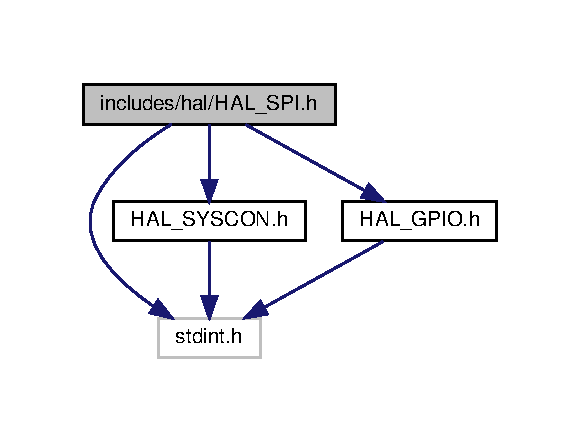
\includegraphics[width=279pt]{HAL__SPI_8h__incl}
\end{center}
\end{figure}
\subsection*{Estructuras de datos}
\begin{DoxyCompactItemize}
\item 
struct \hyperlink{structhal__spi__master__mode__config__t}{hal\+\_\+spi\+\_\+master\+\_\+mode\+\_\+config\+\_\+t}
\item 
struct \hyperlink{HAL__SPI_8h_structhal__spi__master__mode__tx__config__t}{hal\+\_\+spi\+\_\+master\+\_\+mode\+\_\+tx\+\_\+config\+\_\+t}
\item 
struct \hyperlink{HAL__SPI_8h_structhal__spi__master__mode__tx__data__t}{hal\+\_\+spi\+\_\+master\+\_\+mode\+\_\+tx\+\_\+data\+\_\+t}
\end{DoxyCompactItemize}
\subsection*{defines}
\begin{DoxyCompactItemize}
\item 
\mbox{\Hypertarget{HAL__SPI_8h_aa155c3ad4568672fbec24698f9e267ad}\label{HAL__SPI_8h_aa155c3ad4568672fbec24698f9e267ad}} 
\#define {\bfseries H\+A\+L\+\_\+\+S\+P\+I\+\_\+\+D\+U\+M\+M\+Y\+\_\+\+B\+Y\+TE}~(0x\+F\+F)
\end{DoxyCompactItemize}
\subsection*{Enumeraciones}
\begin{DoxyCompactItemize}
\item 
\mbox{\Hypertarget{HAL__SPI_8h_af0531d47c7a0508e49c239b8ac94eecb}\label{HAL__SPI_8h_af0531d47c7a0508e49c239b8ac94eecb}} 
enum {\bfseries hal\+\_\+spi\+\_\+sel\+\_\+en} \{ {\bfseries H\+A\+L\+\_\+\+S\+P\+I\+\_\+0} = 0, 
{\bfseries H\+A\+L\+\_\+\+S\+P\+I\+\_\+1}
 \}
\item 
\mbox{\Hypertarget{HAL__SPI_8h_a227108083b750e225901d1e2ee8ba2c1}\label{HAL__SPI_8h_a227108083b750e225901d1e2ee8ba2c1}} 
enum {\bfseries hal\+\_\+spi\+\_\+data\+\_\+length\+\_\+en} \{ \newline
{\bfseries H\+A\+L\+\_\+\+S\+P\+I\+\_\+\+D\+A\+T\+A\+\_\+\+L\+E\+N\+G\+T\+H\+\_\+1\+\_\+\+B\+IT} = 0, 
{\bfseries H\+A\+L\+\_\+\+S\+P\+I\+\_\+\+D\+A\+T\+A\+\_\+\+L\+E\+N\+G\+T\+H\+\_\+2\+\_\+\+B\+IT}, 
{\bfseries H\+A\+L\+\_\+\+S\+P\+I\+\_\+\+D\+A\+T\+A\+\_\+\+L\+E\+N\+G\+T\+H\+\_\+3\+\_\+\+B\+IT}, 
{\bfseries H\+A\+L\+\_\+\+S\+P\+I\+\_\+\+D\+A\+T\+A\+\_\+\+L\+E\+N\+G\+T\+H\+\_\+4\+\_\+\+B\+IT}, 
\newline
{\bfseries H\+A\+L\+\_\+\+S\+P\+I\+\_\+\+D\+A\+T\+A\+\_\+\+L\+E\+N\+G\+T\+H\+\_\+5\+\_\+\+B\+IT}, 
{\bfseries H\+A\+L\+\_\+\+S\+P\+I\+\_\+\+D\+A\+T\+A\+\_\+\+L\+E\+N\+G\+T\+H\+\_\+6\+\_\+\+B\+IT}, 
{\bfseries H\+A\+L\+\_\+\+S\+P\+I\+\_\+\+D\+A\+T\+A\+\_\+\+L\+E\+N\+G\+T\+H\+\_\+7\+\_\+\+B\+IT}, 
{\bfseries H\+A\+L\+\_\+\+S\+P\+I\+\_\+\+D\+A\+T\+A\+\_\+\+L\+E\+N\+G\+T\+H\+\_\+8\+\_\+\+B\+IT}, 
\newline
{\bfseries H\+A\+L\+\_\+\+S\+P\+I\+\_\+\+D\+A\+T\+A\+\_\+\+L\+E\+N\+G\+T\+H\+\_\+9\+\_\+\+B\+IT}, 
{\bfseries H\+A\+L\+\_\+\+S\+P\+I\+\_\+\+D\+A\+T\+A\+\_\+\+L\+E\+N\+G\+T\+H\+\_\+10\+\_\+\+B\+IT}, 
{\bfseries H\+A\+L\+\_\+\+S\+P\+I\+\_\+\+D\+A\+T\+A\+\_\+\+L\+E\+N\+G\+T\+H\+\_\+11\+\_\+\+B\+IT}, 
{\bfseries H\+A\+L\+\_\+\+S\+P\+I\+\_\+\+D\+A\+T\+A\+\_\+\+L\+E\+N\+G\+T\+H\+\_\+12\+\_\+\+B\+IT}, 
\newline
{\bfseries H\+A\+L\+\_\+\+S\+P\+I\+\_\+\+D\+A\+T\+A\+\_\+\+L\+E\+N\+G\+T\+H\+\_\+13\+\_\+\+B\+IT}, 
{\bfseries H\+A\+L\+\_\+\+S\+P\+I\+\_\+\+D\+A\+T\+A\+\_\+\+L\+E\+N\+G\+T\+H\+\_\+14\+\_\+\+B\+IT}, 
{\bfseries H\+A\+L\+\_\+\+S\+P\+I\+\_\+\+D\+A\+T\+A\+\_\+\+L\+E\+N\+G\+T\+H\+\_\+15\+\_\+\+B\+IT}, 
{\bfseries H\+A\+L\+\_\+\+S\+P\+I\+\_\+\+D\+A\+T\+A\+\_\+\+L\+E\+N\+G\+T\+H\+\_\+16\+\_\+\+B\+IT}
 \}
\item 
\mbox{\Hypertarget{HAL__SPI_8h_abe5c2177f6baea2b1eb394325a11f8d3}\label{HAL__SPI_8h_abe5c2177f6baea2b1eb394325a11f8d3}} 
enum {\bfseries hal\+\_\+spi\+\_\+clock\+\_\+mode\+\_\+en} \{ {\bfseries H\+A\+L\+\_\+\+S\+P\+I\+\_\+\+C\+L\+O\+C\+K\+\_\+\+M\+O\+D\+E\+\_\+0} = 0, 
{\bfseries H\+A\+L\+\_\+\+S\+P\+I\+\_\+\+C\+L\+O\+C\+K\+\_\+\+M\+O\+D\+E\+\_\+1}, 
{\bfseries H\+A\+L\+\_\+\+S\+P\+I\+\_\+\+C\+L\+O\+C\+K\+\_\+\+M\+O\+D\+E\+\_\+2}, 
{\bfseries H\+A\+L\+\_\+\+S\+P\+I\+\_\+\+C\+L\+O\+C\+K\+\_\+\+M\+O\+D\+E\+\_\+3}
 \}
\item 
\mbox{\Hypertarget{HAL__SPI_8h_ae4b694f0781b20b8c818d568fe39f20f}\label{HAL__SPI_8h_ae4b694f0781b20b8c818d568fe39f20f}} 
enum {\bfseries hal\+\_\+spi\+\_\+ssel\+\_\+polarity\+\_\+en} \{ {\bfseries H\+A\+L\+\_\+\+S\+P\+I\+\_\+\+S\+S\+E\+L\+\_\+\+P\+O\+L\+A\+R\+I\+T\+Y\+\_\+\+L\+OW} = 0, 
{\bfseries H\+A\+L\+\_\+\+S\+P\+I\+\_\+\+S\+S\+E\+L\+\_\+\+P\+O\+L\+A\+R\+I\+T\+Y\+\_\+\+H\+I\+GH}
 \}
\item 
\mbox{\Hypertarget{HAL__SPI_8h_ae079f1e93eaa69c19c037409e48cabaa}\label{HAL__SPI_8h_ae079f1e93eaa69c19c037409e48cabaa}} 
enum {\bfseries hal\+\_\+spi\+\_\+ssel\+\_\+sel\+\_\+en} \{ \newline
{\bfseries H\+A\+L\+\_\+\+S\+P\+I\+\_\+\+S\+S\+E\+L\+\_\+\+S\+E\+L\+E\+C\+T\+I\+O\+N\+\_\+0} = 0, 
{\bfseries H\+A\+L\+\_\+\+S\+P\+I\+\_\+\+S\+S\+E\+L\+\_\+\+S\+E\+L\+E\+C\+T\+I\+O\+N\+\_\+1}, 
{\bfseries H\+A\+L\+\_\+\+S\+P\+I\+\_\+\+S\+S\+E\+L\+\_\+\+S\+E\+L\+E\+C\+T\+I\+O\+N\+\_\+2}, 
{\bfseries H\+A\+L\+\_\+\+S\+P\+I\+\_\+\+S\+S\+E\+L\+\_\+\+S\+E\+L\+E\+C\+T\+I\+O\+N\+\_\+3}, 
\newline
{\bfseries H\+A\+L\+\_\+\+S\+P\+I\+\_\+\+S\+S\+E\+L\+\_\+\+S\+E\+L\+E\+C\+T\+I\+O\+N\+\_\+\+O\+T\+H\+ER}
 \}
\end{DoxyCompactItemize}
\subsection*{Funciones}
\begin{DoxyCompactItemize}
\item 
void \hyperlink{HAL__SPI_8h_a9babc814c41f2d8714551fc9af81d346}{hal\+\_\+spi\+\_\+master\+\_\+mode\+\_\+init} (hal\+\_\+spi\+\_\+sel\+\_\+en inst, const \hyperlink{structhal__spi__master__mode__config__t}{hal\+\_\+spi\+\_\+master\+\_\+mode\+\_\+config\+\_\+t} $\ast$config)
\begin{DoxyCompactList}\small\item\em Inicializar S\+PI en modo master. \end{DoxyCompactList}\item 
uint16\+\_\+t \hyperlink{HAL__SPI_8h_a6ca16392e2331ab9db9d97f3a6358346}{hal\+\_\+spi\+\_\+master\+\_\+mode\+\_\+rx\+\_\+data} (hal\+\_\+spi\+\_\+sel\+\_\+en inst)
\begin{DoxyCompactList}\small\item\em Leer el dato recibido. \end{DoxyCompactList}\item 
void \hyperlink{HAL__SPI_8h_a11b672c8dcef79e8784497b23f1618b7}{hal\+\_\+spi\+\_\+master\+\_\+mode\+\_\+config\+\_\+tx} (hal\+\_\+spi\+\_\+sel\+\_\+en inst, const \hyperlink{HAL__SPI_8h_structhal__spi__master__mode__tx__config__t}{hal\+\_\+spi\+\_\+master\+\_\+mode\+\_\+tx\+\_\+config\+\_\+t} $\ast$config)
\begin{DoxyCompactList}\small\item\em Configurar la transmision. \end{DoxyCompactList}\item 
void \hyperlink{HAL__SPI_8h_ad7cfe819f562f90c6bb07e2577699d86}{hal\+\_\+spi\+\_\+master\+\_\+mode\+\_\+tx\+\_\+data} (hal\+\_\+spi\+\_\+sel\+\_\+en inst, const \hyperlink{HAL__SPI_8h_structhal__spi__master__mode__tx__data__t}{hal\+\_\+spi\+\_\+master\+\_\+mode\+\_\+tx\+\_\+data\+\_\+t} $\ast$data)
\begin{DoxyCompactList}\small\item\em Transmitir dato. \end{DoxyCompactList}\item 
void \hyperlink{HAL__SPI_8h_a5bbc56bb8e86b9b077822fab5297e513}{hal\+\_\+spi\+\_\+master\+\_\+mode\+\_\+register\+\_\+tx\+\_\+callback} (hal\+\_\+spi\+\_\+sel\+\_\+en inst, void($\ast$new\+\_\+callback)(void))
\begin{DoxyCompactList}\small\item\em Actualizar callback en T\+X\+R\+DY. \end{DoxyCompactList}\item 
void \hyperlink{HAL__SPI_8h_a363e7e3be50a625bd8fe6a748c473027}{hal\+\_\+spi\+\_\+master\+\_\+mode\+\_\+register\+\_\+rx\+\_\+callback} (hal\+\_\+spi\+\_\+sel\+\_\+en inst, void($\ast$new\+\_\+callback)(void))
\begin{DoxyCompactList}\small\item\em Actualizar callback en R\+X\+R\+DY. \end{DoxyCompactList}\end{DoxyCompactItemize}


\subsection{Descripción detallada}
Declaraciones a nivel de aplicacion del periferico S\+PI (L\+P\+C845) 

\begin{DoxyAuthor}{Autor}
Augusto Santini 
\end{DoxyAuthor}
\begin{DoxyDate}{Fecha}
3/2020 
\end{DoxyDate}
\begin{DoxyVersion}{Versión}
1.\+0 
\end{DoxyVersion}


\subsection{Documentación de las estructuras de datos}
\index{hal\+\_\+spi\+\_\+master\+\_\+mode\+\_\+tx\+\_\+config\+\_\+t@{hal\+\_\+spi\+\_\+master\+\_\+mode\+\_\+tx\+\_\+config\+\_\+t}}\label{structhal__spi__master__mode__tx__config__t}
\Hypertarget{HAL__SPI_8h_structhal__spi__master__mode__tx__config__t}
\subsubsection{struct hal\+\_\+spi\+\_\+master\+\_\+mode\+\_\+tx\+\_\+config\+\_\+t}
\begin{DoxyFields}{Campos de datos}
\mbox{\Hypertarget{HAL__SPI_8h_af409a6b3ff876d386c8d9b38f05e633c}\label{HAL__SPI_8h_af409a6b3ff876d386c8d9b38f05e633c}} 
hal\_spi\_clock\_mode\_en&
clock\_mode&
\\
\hline

\mbox{\Hypertarget{HAL__SPI_8h_a3f6dc062eedd7440d333341c9fa187fc}\label{HAL__SPI_8h_a3f6dc062eedd7440d333341c9fa187fc}} 
uint16\_t&
clock\_div&
\\
\hline

\end{DoxyFields}
\index{hal\+\_\+spi\+\_\+master\+\_\+mode\+\_\+tx\+\_\+data\+\_\+t@{hal\+\_\+spi\+\_\+master\+\_\+mode\+\_\+tx\+\_\+data\+\_\+t}}\label{structhal__spi__master__mode__tx__data__t}
\Hypertarget{HAL__SPI_8h_structhal__spi__master__mode__tx__data__t}
\subsubsection{struct hal\+\_\+spi\+\_\+master\+\_\+mode\+\_\+tx\+\_\+data\+\_\+t}
\begin{DoxyFields}{Campos de datos}
\mbox{\Hypertarget{HAL__SPI_8h_ace5d9edd50ae7a04c202ce1aa9ffc9d1}\label{HAL__SPI_8h_ace5d9edd50ae7a04c202ce1aa9ffc9d1}} 
uint32\_t&
data: 16&
\\
\hline

\mbox{\Hypertarget{HAL__SPI_8h_aaab3fc186c57a63900f5993863c07c4a}\label{HAL__SPI_8h_aaab3fc186c57a63900f5993863c07c4a}} 
uint32\_t&
ssel0\_n: 1&
\\
\hline

\mbox{\Hypertarget{HAL__SPI_8h_a48d1d2904f75bc7168ff179a3aeb104d}\label{HAL__SPI_8h_a48d1d2904f75bc7168ff179a3aeb104d}} 
uint32\_t&
ssel1\_n: 1&
\\
\hline

\mbox{\Hypertarget{HAL__SPI_8h_a6f213524ceb263d64b63185d52638901}\label{HAL__SPI_8h_a6f213524ceb263d64b63185d52638901}} 
uint32\_t&
ssel2\_n: 1&
\\
\hline

\mbox{\Hypertarget{HAL__SPI_8h_adc9f4bc3389a51df667606fc05ab7b20}\label{HAL__SPI_8h_adc9f4bc3389a51df667606fc05ab7b20}} 
uint32\_t&
ssel3\_n: 1&
\\
\hline

\mbox{\Hypertarget{HAL__SPI_8h_af150436bf862f82b00a2e7b759684a74}\label{HAL__SPI_8h_af150436bf862f82b00a2e7b759684a74}} 
uint32\_t&
eot: 1&
\\
\hline

\mbox{\Hypertarget{HAL__SPI_8h_a01f721e64eb8c6d026cbbdf42e85da2b}\label{HAL__SPI_8h_a01f721e64eb8c6d026cbbdf42e85da2b}} 
uint32\_t&
eof: 1&
\\
\hline

\mbox{\Hypertarget{HAL__SPI_8h_a0ea6f255ed33e8bc7af80de3dec62e65}\label{HAL__SPI_8h_a0ea6f255ed33e8bc7af80de3dec62e65}} 
uint32\_t&
rxignore: 1&
\\
\hline

\mbox{\Hypertarget{HAL__SPI_8h_a34120f9ce21c6560bd05d5b0cbcf6b3c}\label{HAL__SPI_8h_a34120f9ce21c6560bd05d5b0cbcf6b3c}} 
uint32\_t&
\_\_pad0\_\_: 1&
\\
\hline

\mbox{\Hypertarget{HAL__SPI_8h_a63c569f0b77034323eb485a9c67d4956}\label{HAL__SPI_8h_a63c569f0b77034323eb485a9c67d4956}} 
uint32\_t&
data\_length: 4&
\\
\hline

\mbox{\Hypertarget{HAL__SPI_8h_a5374a84b23db0afe275be7797c8f74b0}\label{HAL__SPI_8h_a5374a84b23db0afe275be7797c8f74b0}} 
uint32\_t&
\_\_pad1\_\_: 4&
\\
\hline

\end{DoxyFields}


\subsection{Documentación de las funciones}
\mbox{\Hypertarget{HAL__SPI_8h_a9babc814c41f2d8714551fc9af81d346}\label{HAL__SPI_8h_a9babc814c41f2d8714551fc9af81d346}} 
\index{H\+A\+L\+\_\+\+S\+P\+I.\+h@{H\+A\+L\+\_\+\+S\+P\+I.\+h}!hal\+\_\+spi\+\_\+master\+\_\+mode\+\_\+init@{hal\+\_\+spi\+\_\+master\+\_\+mode\+\_\+init}}
\index{hal\+\_\+spi\+\_\+master\+\_\+mode\+\_\+init@{hal\+\_\+spi\+\_\+master\+\_\+mode\+\_\+init}!H\+A\+L\+\_\+\+S\+P\+I.\+h@{H\+A\+L\+\_\+\+S\+P\+I.\+h}}
\subsubsection{\texorpdfstring{hal\+\_\+spi\+\_\+master\+\_\+mode\+\_\+init()}{hal\_spi\_master\_mode\_init()}}
{\footnotesize\ttfamily void hal\+\_\+spi\+\_\+master\+\_\+mode\+\_\+init (\begin{DoxyParamCaption}\item[{hal\+\_\+spi\+\_\+sel\+\_\+en}]{inst,  }\item[{const \hyperlink{structhal__spi__master__mode__config__t}{hal\+\_\+spi\+\_\+master\+\_\+mode\+\_\+config\+\_\+t} $\ast$}]{config }\end{DoxyParamCaption})}



Inicializar S\+PI en modo master. 


\begin{DoxyParams}[1]{Parámetros}
\mbox{\tt in}  & {\em inst} & Instancia de S\+PI a inicializar \\
\hline
\mbox{\tt in}  & {\em config} & Configuracion deseada \\
\hline
\end{DoxyParams}
\mbox{\Hypertarget{HAL__SPI_8h_a6ca16392e2331ab9db9d97f3a6358346}\label{HAL__SPI_8h_a6ca16392e2331ab9db9d97f3a6358346}} 
\index{H\+A\+L\+\_\+\+S\+P\+I.\+h@{H\+A\+L\+\_\+\+S\+P\+I.\+h}!hal\+\_\+spi\+\_\+master\+\_\+mode\+\_\+rx\+\_\+data@{hal\+\_\+spi\+\_\+master\+\_\+mode\+\_\+rx\+\_\+data}}
\index{hal\+\_\+spi\+\_\+master\+\_\+mode\+\_\+rx\+\_\+data@{hal\+\_\+spi\+\_\+master\+\_\+mode\+\_\+rx\+\_\+data}!H\+A\+L\+\_\+\+S\+P\+I.\+h@{H\+A\+L\+\_\+\+S\+P\+I.\+h}}
\subsubsection{\texorpdfstring{hal\+\_\+spi\+\_\+master\+\_\+mode\+\_\+rx\+\_\+data()}{hal\_spi\_master\_mode\_rx\_data()}}
{\footnotesize\ttfamily uint16\+\_\+t hal\+\_\+spi\+\_\+master\+\_\+mode\+\_\+rx\+\_\+data (\begin{DoxyParamCaption}\item[{hal\+\_\+spi\+\_\+sel\+\_\+en}]{inst }\end{DoxyParamCaption})}



Leer el dato recibido. 


\begin{DoxyParams}[1]{Parámetros}
\mbox{\tt in}  & {\em inst} & Instancia a consultar \\
\hline
\end{DoxyParams}
\begin{DoxyReturn}{Devuelve}
Dato recibido 
\end{DoxyReturn}
\mbox{\Hypertarget{HAL__SPI_8h_a11b672c8dcef79e8784497b23f1618b7}\label{HAL__SPI_8h_a11b672c8dcef79e8784497b23f1618b7}} 
\index{H\+A\+L\+\_\+\+S\+P\+I.\+h@{H\+A\+L\+\_\+\+S\+P\+I.\+h}!hal\+\_\+spi\+\_\+master\+\_\+mode\+\_\+config\+\_\+tx@{hal\+\_\+spi\+\_\+master\+\_\+mode\+\_\+config\+\_\+tx}}
\index{hal\+\_\+spi\+\_\+master\+\_\+mode\+\_\+config\+\_\+tx@{hal\+\_\+spi\+\_\+master\+\_\+mode\+\_\+config\+\_\+tx}!H\+A\+L\+\_\+\+S\+P\+I.\+h@{H\+A\+L\+\_\+\+S\+P\+I.\+h}}
\subsubsection{\texorpdfstring{hal\+\_\+spi\+\_\+master\+\_\+mode\+\_\+config\+\_\+tx()}{hal\_spi\_master\_mode\_config\_tx()}}
{\footnotesize\ttfamily void hal\+\_\+spi\+\_\+master\+\_\+mode\+\_\+config\+\_\+tx (\begin{DoxyParamCaption}\item[{hal\+\_\+spi\+\_\+sel\+\_\+en}]{inst,  }\item[{const \hyperlink{HAL__SPI_8h_structhal__spi__master__mode__tx__config__t}{hal\+\_\+spi\+\_\+master\+\_\+mode\+\_\+tx\+\_\+config\+\_\+t} $\ast$}]{config }\end{DoxyParamCaption})}



Configurar la transmision. 


\begin{DoxyParams}[1]{Parámetros}
\mbox{\tt in}  & {\em inst} & Instancia a configurar \\
\hline
\mbox{\tt in}  & {\em config} & Configuracion para la transmision deseada \\
\hline
\end{DoxyParams}
\mbox{\Hypertarget{HAL__SPI_8h_ad7cfe819f562f90c6bb07e2577699d86}\label{HAL__SPI_8h_ad7cfe819f562f90c6bb07e2577699d86}} 
\index{H\+A\+L\+\_\+\+S\+P\+I.\+h@{H\+A\+L\+\_\+\+S\+P\+I.\+h}!hal\+\_\+spi\+\_\+master\+\_\+mode\+\_\+tx\+\_\+data@{hal\+\_\+spi\+\_\+master\+\_\+mode\+\_\+tx\+\_\+data}}
\index{hal\+\_\+spi\+\_\+master\+\_\+mode\+\_\+tx\+\_\+data@{hal\+\_\+spi\+\_\+master\+\_\+mode\+\_\+tx\+\_\+data}!H\+A\+L\+\_\+\+S\+P\+I.\+h@{H\+A\+L\+\_\+\+S\+P\+I.\+h}}
\subsubsection{\texorpdfstring{hal\+\_\+spi\+\_\+master\+\_\+mode\+\_\+tx\+\_\+data()}{hal\_spi\_master\_mode\_tx\_data()}}
{\footnotesize\ttfamily void hal\+\_\+spi\+\_\+master\+\_\+mode\+\_\+tx\+\_\+data (\begin{DoxyParamCaption}\item[{hal\+\_\+spi\+\_\+sel\+\_\+en}]{inst,  }\item[{const \hyperlink{HAL__SPI_8h_structhal__spi__master__mode__tx__data__t}{hal\+\_\+spi\+\_\+master\+\_\+mode\+\_\+tx\+\_\+data\+\_\+t} $\ast$}]{data }\end{DoxyParamCaption})}



Transmitir dato. 


\begin{DoxyParams}[1]{Parámetros}
\mbox{\tt in}  & {\em inst} & Instancia a utilizar \\
\hline
\mbox{\tt in}  & {\em data} & Dato a transmitir, con controles asociados \\
\hline
\end{DoxyParams}
\mbox{\Hypertarget{HAL__SPI_8h_a5bbc56bb8e86b9b077822fab5297e513}\label{HAL__SPI_8h_a5bbc56bb8e86b9b077822fab5297e513}} 
\index{H\+A\+L\+\_\+\+S\+P\+I.\+h@{H\+A\+L\+\_\+\+S\+P\+I.\+h}!hal\+\_\+spi\+\_\+master\+\_\+mode\+\_\+register\+\_\+tx\+\_\+callback@{hal\+\_\+spi\+\_\+master\+\_\+mode\+\_\+register\+\_\+tx\+\_\+callback}}
\index{hal\+\_\+spi\+\_\+master\+\_\+mode\+\_\+register\+\_\+tx\+\_\+callback@{hal\+\_\+spi\+\_\+master\+\_\+mode\+\_\+register\+\_\+tx\+\_\+callback}!H\+A\+L\+\_\+\+S\+P\+I.\+h@{H\+A\+L\+\_\+\+S\+P\+I.\+h}}
\subsubsection{\texorpdfstring{hal\+\_\+spi\+\_\+master\+\_\+mode\+\_\+register\+\_\+tx\+\_\+callback()}{hal\_spi\_master\_mode\_register\_tx\_callback()}}
{\footnotesize\ttfamily void hal\+\_\+spi\+\_\+master\+\_\+mode\+\_\+register\+\_\+tx\+\_\+callback (\begin{DoxyParamCaption}\item[{hal\+\_\+spi\+\_\+sel\+\_\+en}]{inst,  }\item[{void($\ast$)(void)}]{new\+\_\+callback }\end{DoxyParamCaption})}



Actualizar callback en T\+X\+R\+DY. 


\begin{DoxyParams}[1]{Parámetros}
\mbox{\tt in}  & {\em inst} & Instancia a configurar \\
\hline
\mbox{\tt in}  & {\em new\+\_\+callback} & Nuevo callback a ejecutar en T\+X\+R\+DY \\
\hline
\end{DoxyParams}
\mbox{\Hypertarget{HAL__SPI_8h_a363e7e3be50a625bd8fe6a748c473027}\label{HAL__SPI_8h_a363e7e3be50a625bd8fe6a748c473027}} 
\index{H\+A\+L\+\_\+\+S\+P\+I.\+h@{H\+A\+L\+\_\+\+S\+P\+I.\+h}!hal\+\_\+spi\+\_\+master\+\_\+mode\+\_\+register\+\_\+rx\+\_\+callback@{hal\+\_\+spi\+\_\+master\+\_\+mode\+\_\+register\+\_\+rx\+\_\+callback}}
\index{hal\+\_\+spi\+\_\+master\+\_\+mode\+\_\+register\+\_\+rx\+\_\+callback@{hal\+\_\+spi\+\_\+master\+\_\+mode\+\_\+register\+\_\+rx\+\_\+callback}!H\+A\+L\+\_\+\+S\+P\+I.\+h@{H\+A\+L\+\_\+\+S\+P\+I.\+h}}
\subsubsection{\texorpdfstring{hal\+\_\+spi\+\_\+master\+\_\+mode\+\_\+register\+\_\+rx\+\_\+callback()}{hal\_spi\_master\_mode\_register\_rx\_callback()}}
{\footnotesize\ttfamily void hal\+\_\+spi\+\_\+master\+\_\+mode\+\_\+register\+\_\+rx\+\_\+callback (\begin{DoxyParamCaption}\item[{hal\+\_\+spi\+\_\+sel\+\_\+en}]{inst,  }\item[{void($\ast$)(void)}]{new\+\_\+callback }\end{DoxyParamCaption})}



Actualizar callback en R\+X\+R\+DY. 


\begin{DoxyParams}[1]{Parámetros}
\mbox{\tt in}  & {\em inst} & Instancia a configurar \\
\hline
\mbox{\tt in}  & {\em new\+\_\+callback} & Nuevo callback a ejecutar en R\+X\+R\+DY \\
\hline
\end{DoxyParams}

\hypertarget{HAL__SYSCON_8h}{}\section{Referencia del Archivo includes/hal/\+H\+A\+L\+\_\+\+S\+Y\+S\+C\+ON.h}
\label{HAL__SYSCON_8h}\index{includes/hal/\+H\+A\+L\+\_\+\+S\+Y\+S\+C\+O\+N.\+h@{includes/hal/\+H\+A\+L\+\_\+\+S\+Y\+S\+C\+O\+N.\+h}}


Declaraciones a nivel de aplicacion del periferico S\+Y\+S\+C\+ON (L\+P\+C845)  


{\ttfamily \#include $<$stdint.\+h$>$}\newline
Dependencia gráfica adjunta para H\+A\+L\+\_\+\+S\+Y\+S\+C\+O\+N.\+h\+:\nopagebreak
\begin{figure}[H]
\begin{center}
\leavevmode
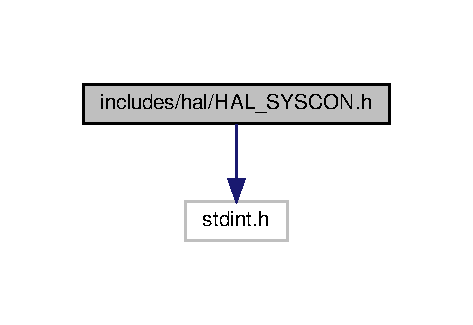
\includegraphics[width=227pt]{HAL__SYSCON_8h__incl}
\end{center}
\end{figure}
Gráfico de los archivos que directa o indirectamente incluyen a este archivo\+:\nopagebreak
\begin{figure}[H]
\begin{center}
\leavevmode
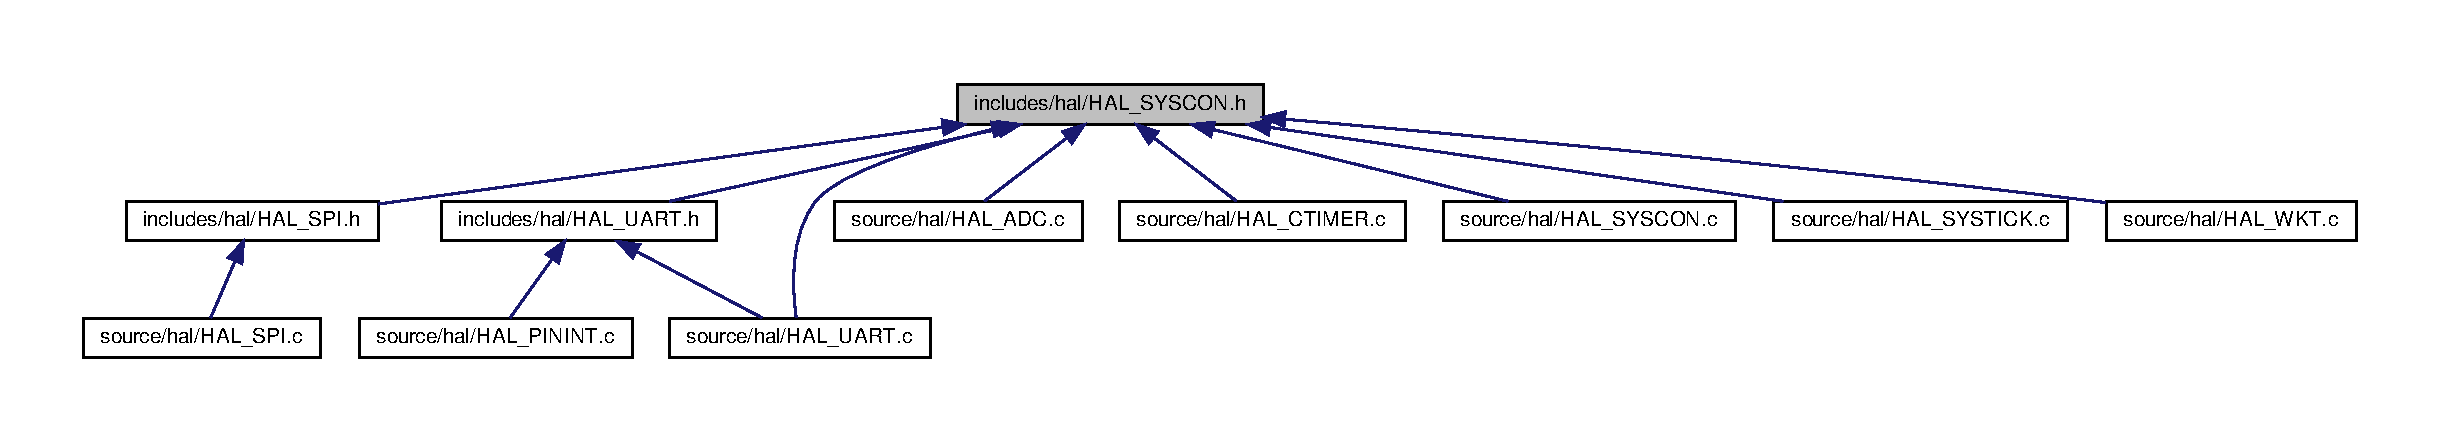
\includegraphics[width=350pt]{HAL__SYSCON_8h__dep__incl}
\end{center}
\end{figure}
\subsection*{Enumeraciones}
\begin{DoxyCompactItemize}
\item 
\mbox{\Hypertarget{HAL__SYSCON_8h_aa23b6654979f5c5d0c6caec99cc336b4}\label{HAL__SYSCON_8h_aa23b6654979f5c5d0c6caec99cc336b4}} 
enum {\bfseries hal\+\_\+syscon\+\_\+clkout\+\_\+source\+\_\+sel\+\_\+en} \{ \newline
{\bfseries H\+A\+L\+\_\+\+S\+Y\+S\+C\+O\+N\+\_\+\+C\+L\+K\+O\+U\+T\+\_\+\+S\+O\+U\+R\+C\+E\+\_\+\+S\+E\+L\+\_\+\+F\+RO} = 0, 
{\bfseries H\+A\+L\+\_\+\+S\+Y\+S\+C\+O\+N\+\_\+\+C\+L\+K\+O\+U\+T\+\_\+\+S\+O\+U\+R\+C\+E\+\_\+\+S\+E\+L\+\_\+\+M\+A\+I\+N\+\_\+\+C\+L\+O\+CK}, 
{\bfseries H\+A\+L\+\_\+\+S\+Y\+S\+C\+O\+N\+\_\+\+C\+L\+K\+O\+U\+T\+\_\+\+S\+O\+U\+R\+C\+E\+\_\+\+S\+E\+L\+\_\+\+S\+Y\+S\+\_\+\+P\+LL}, 
{\bfseries H\+A\+L\+\_\+\+S\+Y\+S\+C\+O\+N\+\_\+\+C\+L\+K\+O\+U\+T\+\_\+\+S\+O\+U\+R\+C\+E\+\_\+\+S\+E\+L\+\_\+\+E\+X\+T\+\_\+\+C\+L\+O\+CK}, 
\newline
{\bfseries H\+A\+L\+\_\+\+S\+Y\+S\+C\+O\+N\+\_\+\+C\+L\+K\+O\+U\+T\+\_\+\+S\+O\+U\+R\+C\+E\+\_\+\+S\+E\+L\+\_\+\+W\+A\+T\+C\+H\+D\+O\+G\+\_\+\+O\+SC}
 \}
\item 
\mbox{\Hypertarget{HAL__SYSCON_8h_ac3c6c02a963d446ae8e9b7c0a71ccdcb}\label{HAL__SYSCON_8h_ac3c6c02a963d446ae8e9b7c0a71ccdcb}} 
enum {\bfseries hal\+\_\+syscon\+\_\+frg\+\_\+clock\+\_\+sel\+\_\+en} \{ {\bfseries H\+A\+L\+\_\+\+S\+Y\+S\+C\+O\+N\+\_\+\+F\+R\+G\+\_\+\+C\+L\+O\+C\+K\+\_\+\+S\+E\+L\+\_\+\+F\+RO} = 0, 
{\bfseries H\+A\+L\+\_\+\+S\+Y\+S\+C\+O\+N\+\_\+\+F\+R\+G\+\_\+\+C\+L\+O\+C\+K\+\_\+\+S\+E\+L\+\_\+\+M\+A\+I\+N\+\_\+\+C\+L\+O\+CK}, 
{\bfseries H\+A\+L\+\_\+\+S\+Y\+S\+C\+O\+N\+\_\+\+F\+R\+G\+\_\+\+C\+L\+O\+C\+K\+\_\+\+S\+E\+L\+\_\+\+S\+Y\+S\+\_\+\+P\+LL}, 
{\bfseries H\+A\+L\+\_\+\+S\+Y\+S\+C\+O\+N\+\_\+\+F\+R\+G\+\_\+\+C\+L\+O\+C\+K\+\_\+\+S\+E\+L\+\_\+\+N\+O\+NE}
 \}
\item 
\mbox{\Hypertarget{HAL__SYSCON_8h_a8f85b75727e34f8c9f8d3c46b44a0ae0}\label{HAL__SYSCON_8h_a8f85b75727e34f8c9f8d3c46b44a0ae0}} 
enum {\bfseries hal\+\_\+syscon\+\_\+peripheral\+\_\+sel\+\_\+en} \{ \newline
{\bfseries H\+A\+L\+\_\+\+S\+Y\+S\+C\+O\+N\+\_\+\+P\+E\+R\+I\+P\+H\+E\+R\+A\+L\+\_\+\+S\+E\+L\+\_\+\+U\+A\+R\+T0} = 0, 
{\bfseries H\+A\+L\+\_\+\+S\+Y\+S\+C\+O\+N\+\_\+\+P\+E\+R\+I\+P\+H\+E\+R\+A\+L\+\_\+\+S\+E\+L\+\_\+\+U\+A\+R\+T1}, 
{\bfseries H\+A\+L\+\_\+\+S\+Y\+S\+C\+O\+N\+\_\+\+P\+E\+R\+I\+P\+H\+E\+R\+A\+L\+\_\+\+S\+E\+L\+\_\+\+U\+A\+R\+T2}, 
{\bfseries H\+A\+L\+\_\+\+S\+Y\+S\+C\+O\+N\+\_\+\+P\+E\+R\+I\+P\+H\+E\+R\+A\+L\+\_\+\+S\+E\+L\+\_\+\+U\+A\+R\+T3}, 
\newline
{\bfseries H\+A\+L\+\_\+\+S\+Y\+S\+C\+O\+N\+\_\+\+P\+E\+R\+I\+P\+H\+E\+R\+A\+L\+\_\+\+S\+E\+L\+\_\+\+U\+A\+R\+T4}, 
{\bfseries H\+A\+L\+\_\+\+S\+Y\+S\+C\+O\+N\+\_\+\+P\+E\+R\+I\+P\+H\+E\+R\+A\+L\+\_\+\+S\+E\+L\+\_\+\+I\+I\+C0}, 
{\bfseries H\+A\+L\+\_\+\+S\+Y\+S\+C\+O\+N\+\_\+\+P\+E\+R\+I\+P\+H\+E\+R\+A\+L\+\_\+\+S\+E\+L\+\_\+\+I\+I\+C1}, 
{\bfseries H\+A\+L\+\_\+\+S\+Y\+S\+C\+O\+N\+\_\+\+P\+E\+R\+I\+P\+H\+E\+R\+A\+L\+\_\+\+S\+E\+L\+\_\+\+I\+I\+C2}, 
\newline
{\bfseries H\+A\+L\+\_\+\+S\+Y\+S\+C\+O\+N\+\_\+\+P\+E\+R\+I\+P\+H\+E\+R\+A\+L\+\_\+\+S\+E\+L\+\_\+\+I\+I\+C3}, 
{\bfseries H\+A\+L\+\_\+\+S\+Y\+S\+C\+O\+N\+\_\+\+P\+E\+R\+I\+P\+H\+E\+R\+A\+L\+\_\+\+S\+E\+L\+\_\+\+S\+P\+I0}, 
{\bfseries H\+A\+L\+\_\+\+S\+Y\+S\+C\+O\+N\+\_\+\+P\+E\+R\+I\+P\+H\+E\+R\+A\+L\+\_\+\+S\+E\+L\+\_\+\+S\+P\+I1}
 \}
\item 
\mbox{\Hypertarget{HAL__SYSCON_8h_a8d1873ed52eb0449a0c12acadcecd47b}\label{HAL__SYSCON_8h_a8d1873ed52eb0449a0c12acadcecd47b}} 
enum {\bfseries hal\+\_\+syscon\+\_\+peripheral\+\_\+clock\+\_\+sel\+\_\+en} \{ \newline
{\bfseries H\+A\+L\+\_\+\+S\+Y\+S\+C\+O\+N\+\_\+\+P\+E\+R\+I\+P\+H\+E\+R\+A\+L\+\_\+\+C\+L\+O\+C\+K\+\_\+\+S\+E\+L\+\_\+\+F\+RO} = 0, 
{\bfseries H\+A\+L\+\_\+\+S\+Y\+S\+C\+O\+N\+\_\+\+P\+E\+R\+I\+P\+H\+E\+R\+A\+L\+\_\+\+C\+L\+O\+C\+K\+\_\+\+S\+E\+L\+\_\+\+M\+A\+IN}, 
{\bfseries H\+A\+L\+\_\+\+S\+Y\+S\+C\+O\+N\+\_\+\+P\+E\+R\+I\+P\+H\+E\+R\+A\+L\+\_\+\+C\+L\+O\+C\+K\+\_\+\+S\+E\+L\+\_\+\+F\+R\+G0}, 
{\bfseries H\+A\+L\+\_\+\+S\+Y\+S\+C\+O\+N\+\_\+\+P\+E\+R\+I\+P\+H\+E\+R\+A\+L\+\_\+\+C\+L\+O\+C\+K\+\_\+\+S\+E\+L\+\_\+\+F\+R\+G1}, 
\newline
{\bfseries H\+A\+L\+\_\+\+S\+Y\+S\+C\+O\+N\+\_\+\+P\+E\+R\+I\+P\+H\+E\+R\+A\+L\+\_\+\+C\+L\+O\+C\+K\+\_\+\+S\+E\+L\+\_\+\+F\+R\+O\+\_\+\+D\+IV}, 
{\bfseries H\+A\+L\+\_\+\+S\+Y\+S\+C\+O\+N\+\_\+\+P\+E\+R\+I\+P\+H\+E\+R\+A\+L\+\_\+\+C\+L\+O\+C\+K\+\_\+\+S\+E\+L\+\_\+\+N\+O\+NE} = 7
 \}
\item 
\mbox{\Hypertarget{HAL__SYSCON_8h_ae6e947aa2e205fb9998ee49ed34314d4}\label{HAL__SYSCON_8h_ae6e947aa2e205fb9998ee49ed34314d4}} 
enum {\bfseries hal\+\_\+syscon\+\_\+iocon\+\_\+glitch\+\_\+sel\+\_\+en} \{ \newline
{\bfseries H\+A\+L\+\_\+\+S\+Y\+S\+C\+O\+N\+\_\+\+I\+O\+C\+O\+N\+\_\+\+G\+L\+I\+T\+C\+H\+\_\+\+S\+E\+L\+\_\+0} = 0, 
{\bfseries H\+A\+L\+\_\+\+S\+Y\+S\+C\+O\+N\+\_\+\+I\+O\+C\+O\+N\+\_\+\+G\+L\+I\+T\+C\+H\+\_\+\+S\+E\+L\+\_\+1}, 
{\bfseries H\+A\+L\+\_\+\+S\+Y\+S\+C\+O\+N\+\_\+\+I\+O\+C\+O\+N\+\_\+\+G\+L\+I\+T\+C\+H\+\_\+\+S\+E\+L\+\_\+2}, 
{\bfseries H\+A\+L\+\_\+\+S\+Y\+S\+C\+O\+N\+\_\+\+I\+O\+C\+O\+N\+\_\+\+G\+L\+I\+T\+C\+H\+\_\+\+S\+E\+L\+\_\+3}, 
\newline
{\bfseries H\+A\+L\+\_\+\+S\+Y\+S\+C\+O\+N\+\_\+\+I\+O\+C\+O\+N\+\_\+\+G\+L\+I\+T\+C\+H\+\_\+\+S\+E\+L\+\_\+4}, 
{\bfseries H\+A\+L\+\_\+\+S\+Y\+S\+C\+O\+N\+\_\+\+I\+O\+C\+O\+N\+\_\+\+G\+L\+I\+T\+C\+H\+\_\+\+S\+E\+L\+\_\+5}, 
{\bfseries H\+A\+L\+\_\+\+S\+Y\+S\+C\+O\+N\+\_\+\+I\+O\+C\+O\+N\+\_\+\+G\+L\+I\+T\+C\+H\+\_\+\+S\+E\+L\+\_\+6}, 
{\bfseries H\+A\+L\+\_\+\+S\+Y\+S\+C\+O\+N\+\_\+\+I\+O\+C\+O\+N\+\_\+\+G\+L\+I\+T\+C\+H\+\_\+\+S\+E\+L\+\_\+7}
 \}
\item 
\mbox{\Hypertarget{HAL__SYSCON_8h_af54a8bad7d8d25e0778c0f74ff90a9b2}\label{HAL__SYSCON_8h_af54a8bad7d8d25e0778c0f74ff90a9b2}} 
enum {\bfseries hal\+\_\+syscon\+\_\+pll\+\_\+source\+\_\+sel\+\_\+en} \{ {\bfseries H\+A\+L\+\_\+\+S\+Y\+S\+C\+O\+N\+\_\+\+P\+L\+L\+\_\+\+S\+O\+U\+R\+C\+E\+\_\+\+S\+E\+L\+\_\+\+F\+RO} = 0, 
{\bfseries H\+A\+L\+\_\+\+S\+Y\+S\+C\+O\+N\+\_\+\+P\+L\+L\+\_\+\+S\+O\+U\+R\+C\+E\+\_\+\+S\+E\+L\+\_\+\+E\+X\+T\+\_\+\+C\+LK}, 
{\bfseries H\+A\+L\+\_\+\+S\+Y\+S\+C\+O\+N\+\_\+\+P\+L\+L\+\_\+\+S\+O\+U\+R\+C\+E\+\_\+\+S\+E\+L\+\_\+\+W\+A\+T\+C\+H\+D\+OG}, 
{\bfseries H\+A\+L\+\_\+\+S\+Y\+S\+C\+O\+N\+\_\+\+P\+L\+L\+\_\+\+S\+O\+U\+R\+C\+E\+\_\+\+S\+E\+L\+\_\+\+F\+R\+O\+\_\+\+D\+IV}
 \}
\end{DoxyCompactItemize}
\subsection*{Funciones}
\begin{DoxyCompactItemize}
\item 
uint32\+\_\+t \hyperlink{HAL__SYSCON_8h_a31c48c74f760fbad8518a0a6c89731eb}{hal\+\_\+syscon\+\_\+get\+\_\+system\+\_\+clock} (void)
\begin{DoxyCompactList}\small\item\em Obtener la frecuencia actual del main clock. \end{DoxyCompactList}\item 
uint32\+\_\+t \hyperlink{HAL__SYSCON_8h_a7768b17907648deb424cb4254ad35d10}{hal\+\_\+syscon\+\_\+get\+\_\+fro\+\_\+clock} (void)
\begin{DoxyCompactList}\small\item\em Obtener la frecuencia actual del F\+RO. \end{DoxyCompactList}\item 
void \hyperlink{HAL__SYSCON_8h_accafad7cb2378e99a09afd26de8d432e}{hal\+\_\+syscon\+\_\+config\+\_\+external\+\_\+crystal} (uint32\+\_\+t crystal\+\_\+freq, uint8\+\_\+t use\+\_\+as\+\_\+main)
\begin{DoxyCompactList}\small\item\em Configurar el ext clock a partir de un cristal externo. \end{DoxyCompactList}\item 
void \hyperlink{HAL__SYSCON_8h_ab6b37d2df55c51dbb27c2c02bb087587}{hal\+\_\+syscon\+\_\+config\+\_\+fro\+\_\+direct} (uint8\+\_\+t direct, uint8\+\_\+t use\+\_\+as\+\_\+main)
\begin{DoxyCompactList}\small\item\em Configurar el clock F\+RO. \end{DoxyCompactList}\item 
void \hyperlink{HAL__SYSCON_8h_a1c2a74ef250399dba55e1f17b43abe38}{hal\+\_\+syscon\+\_\+config\+\_\+clkout} (uint8\+\_\+t port, uint8\+\_\+t pin, hal\+\_\+syscon\+\_\+clkout\+\_\+source\+\_\+sel\+\_\+en clock\+\_\+source, uint8\+\_\+t divider)
\begin{DoxyCompactList}\small\item\em Configurar el pin de clock out (salida de clock hacia afuera) \end{DoxyCompactList}\item 
void \hyperlink{HAL__SYSCON_8h_a5cd176b5be324489a45a8626ec89ce99}{hal\+\_\+syscon\+\_\+config\+\_\+frg} (uint8\+\_\+t inst, hal\+\_\+syscon\+\_\+frg\+\_\+clock\+\_\+sel\+\_\+en clock\+\_\+source, uint32\+\_\+t mul)
\begin{DoxyCompactList}\small\item\em Configurar el divisor fraccional. \end{DoxyCompactList}\item 
void \hyperlink{HAL__SYSCON_8h_aeec2e4ffb8eca74db67bd0ce4c7a06c6}{hal\+\_\+syscon\+\_\+set\+\_\+peripheral\+\_\+clock\+\_\+source} (hal\+\_\+syscon\+\_\+peripheral\+\_\+sel\+\_\+en peripheral, hal\+\_\+syscon\+\_\+peripheral\+\_\+clock\+\_\+sel\+\_\+en clock\+\_\+source)
\begin{DoxyCompactList}\small\item\em Fijar la fuente de clock de un periferico. \end{DoxyCompactList}\item 
uint32\+\_\+t \hyperlink{HAL__SYSCON_8h_ac37805288fe2b5489e7f1d1c5765e298}{hal\+\_\+syscon\+\_\+get\+\_\+peripheral\+\_\+clock} (hal\+\_\+syscon\+\_\+peripheral\+\_\+sel\+\_\+en peripheral)
\begin{DoxyCompactList}\small\item\em Obtener la frecuencia de clock en Hz configurada para cierto periferico. \end{DoxyCompactList}\item 
void \hyperlink{HAL__SYSCON_8h_ac2eb2b4b2c904d02fac721092422edeb}{hal\+\_\+syscon\+\_\+set\+\_\+iocon\+\_\+glitch\+\_\+divider} (hal\+\_\+syscon\+\_\+iocon\+\_\+glitch\+\_\+sel\+\_\+en sel, uint32\+\_\+t div)
\begin{DoxyCompactList}\small\item\em Configurar divisor para el clock de glitches del I\+O\+C\+ON. \end{DoxyCompactList}\item 
void \hyperlink{HAL__SYSCON_8h_aa29b349b8b958efeed0831ed31eadf94}{hal\+\_\+syscon\+\_\+config\+\_\+pll} (hal\+\_\+syscon\+\_\+pll\+\_\+source\+\_\+sel\+\_\+en clock\+\_\+source, uint32\+\_\+t freq)
\begin{DoxyCompactList}\small\item\em Configurar el P\+LL. \end{DoxyCompactList}\item 
uint32\+\_\+t \hyperlink{HAL__SYSCON_8h_aadbb4d022ecc8916c0346b8f537e19d0}{hal\+\_\+syscon\+\_\+get\+\_\+pll\+\_\+clock} (void)
\begin{DoxyCompactList}\small\item\em Obtener frecuencia actual configurada del P\+LL. \end{DoxyCompactList}\end{DoxyCompactItemize}


\subsection{Descripción detallada}
Declaraciones a nivel de aplicacion del periferico S\+Y\+S\+C\+ON (L\+P\+C845) 

\begin{DoxyAuthor}{Autor}
Augusto Santini 
\end{DoxyAuthor}
\begin{DoxyDate}{Fecha}
6/2019 
\end{DoxyDate}
\begin{DoxyVersion}{Versión}
1.\+0 
\end{DoxyVersion}


\subsection{Documentación de las funciones}
\mbox{\Hypertarget{HAL__SYSCON_8h_a31c48c74f760fbad8518a0a6c89731eb}\label{HAL__SYSCON_8h_a31c48c74f760fbad8518a0a6c89731eb}} 
\index{H\+A\+L\+\_\+\+S\+Y\+S\+C\+O\+N.\+h@{H\+A\+L\+\_\+\+S\+Y\+S\+C\+O\+N.\+h}!hal\+\_\+syscon\+\_\+get\+\_\+system\+\_\+clock@{hal\+\_\+syscon\+\_\+get\+\_\+system\+\_\+clock}}
\index{hal\+\_\+syscon\+\_\+get\+\_\+system\+\_\+clock@{hal\+\_\+syscon\+\_\+get\+\_\+system\+\_\+clock}!H\+A\+L\+\_\+\+S\+Y\+S\+C\+O\+N.\+h@{H\+A\+L\+\_\+\+S\+Y\+S\+C\+O\+N.\+h}}
\subsubsection{\texorpdfstring{hal\+\_\+syscon\+\_\+get\+\_\+system\+\_\+clock()}{hal\_syscon\_get\_system\_clock()}}
{\footnotesize\ttfamily uint32\+\_\+t hal\+\_\+syscon\+\_\+get\+\_\+system\+\_\+clock (\begin{DoxyParamCaption}\item[{void}]{ }\end{DoxyParamCaption})}



Obtener la frecuencia actual del main clock. 

\begin{DoxyReturn}{Devuelve}
Frecuencia del main clock en Hz 
\end{DoxyReturn}
\mbox{\Hypertarget{HAL__SYSCON_8h_a7768b17907648deb424cb4254ad35d10}\label{HAL__SYSCON_8h_a7768b17907648deb424cb4254ad35d10}} 
\index{H\+A\+L\+\_\+\+S\+Y\+S\+C\+O\+N.\+h@{H\+A\+L\+\_\+\+S\+Y\+S\+C\+O\+N.\+h}!hal\+\_\+syscon\+\_\+get\+\_\+fro\+\_\+clock@{hal\+\_\+syscon\+\_\+get\+\_\+fro\+\_\+clock}}
\index{hal\+\_\+syscon\+\_\+get\+\_\+fro\+\_\+clock@{hal\+\_\+syscon\+\_\+get\+\_\+fro\+\_\+clock}!H\+A\+L\+\_\+\+S\+Y\+S\+C\+O\+N.\+h@{H\+A\+L\+\_\+\+S\+Y\+S\+C\+O\+N.\+h}}
\subsubsection{\texorpdfstring{hal\+\_\+syscon\+\_\+get\+\_\+fro\+\_\+clock()}{hal\_syscon\_get\_fro\_clock()}}
{\footnotesize\ttfamily uint32\+\_\+t hal\+\_\+syscon\+\_\+get\+\_\+fro\+\_\+clock (\begin{DoxyParamCaption}\item[{void}]{ }\end{DoxyParamCaption})}



Obtener la frecuencia actual del F\+RO. 

\begin{DoxyReturn}{Devuelve}
Frecuencia del F\+RO en Hz 
\end{DoxyReturn}
\mbox{\Hypertarget{HAL__SYSCON_8h_accafad7cb2378e99a09afd26de8d432e}\label{HAL__SYSCON_8h_accafad7cb2378e99a09afd26de8d432e}} 
\index{H\+A\+L\+\_\+\+S\+Y\+S\+C\+O\+N.\+h@{H\+A\+L\+\_\+\+S\+Y\+S\+C\+O\+N.\+h}!hal\+\_\+syscon\+\_\+config\+\_\+external\+\_\+crystal@{hal\+\_\+syscon\+\_\+config\+\_\+external\+\_\+crystal}}
\index{hal\+\_\+syscon\+\_\+config\+\_\+external\+\_\+crystal@{hal\+\_\+syscon\+\_\+config\+\_\+external\+\_\+crystal}!H\+A\+L\+\_\+\+S\+Y\+S\+C\+O\+N.\+h@{H\+A\+L\+\_\+\+S\+Y\+S\+C\+O\+N.\+h}}
\subsubsection{\texorpdfstring{hal\+\_\+syscon\+\_\+config\+\_\+external\+\_\+crystal()}{hal\_syscon\_config\_external\_crystal()}}
{\footnotesize\ttfamily void hal\+\_\+syscon\+\_\+config\+\_\+external\+\_\+crystal (\begin{DoxyParamCaption}\item[{uint32\+\_\+t}]{crystal\+\_\+freq,  }\item[{uint8\+\_\+t}]{use\+\_\+as\+\_\+main }\end{DoxyParamCaption})}



Configurar el ext clock a partir de un cristal externo. 


\begin{DoxyParams}[1]{Parámetros}
\mbox{\tt in}  & {\em crystal\+\_\+freq} & Frecuencia del cristal externo utilizado \\
\hline
\mbox{\tt in}  & {\em use\+\_\+as\+\_\+main} & Si es distinto de cero, se utilizara el oscilador a cristal como main clock \\
\hline
\end{DoxyParams}
\mbox{\Hypertarget{HAL__SYSCON_8h_ab6b37d2df55c51dbb27c2c02bb087587}\label{HAL__SYSCON_8h_ab6b37d2df55c51dbb27c2c02bb087587}} 
\index{H\+A\+L\+\_\+\+S\+Y\+S\+C\+O\+N.\+h@{H\+A\+L\+\_\+\+S\+Y\+S\+C\+O\+N.\+h}!hal\+\_\+syscon\+\_\+config\+\_\+fro\+\_\+direct@{hal\+\_\+syscon\+\_\+config\+\_\+fro\+\_\+direct}}
\index{hal\+\_\+syscon\+\_\+config\+\_\+fro\+\_\+direct@{hal\+\_\+syscon\+\_\+config\+\_\+fro\+\_\+direct}!H\+A\+L\+\_\+\+S\+Y\+S\+C\+O\+N.\+h@{H\+A\+L\+\_\+\+S\+Y\+S\+C\+O\+N.\+h}}
\subsubsection{\texorpdfstring{hal\+\_\+syscon\+\_\+config\+\_\+fro\+\_\+direct()}{hal\_syscon\_config\_fro\_direct()}}
{\footnotesize\ttfamily void hal\+\_\+syscon\+\_\+config\+\_\+fro\+\_\+direct (\begin{DoxyParamCaption}\item[{uint8\+\_\+t}]{direct,  }\item[{uint8\+\_\+t}]{use\+\_\+as\+\_\+main }\end{DoxyParamCaption})}



Configurar el clock F\+RO. 


\begin{DoxyParams}[1]{Parámetros}
\mbox{\tt in}  & {\em direct} & Si es distinto de cero se omite el divisor del F\+RO \\
\hline
\mbox{\tt in}  & {\em use\+\_\+as\+\_\+main} & Si es distinto de cero, se utilizara el F\+RO como main clock \\
\hline
\end{DoxyParams}
\mbox{\Hypertarget{HAL__SYSCON_8h_a1c2a74ef250399dba55e1f17b43abe38}\label{HAL__SYSCON_8h_a1c2a74ef250399dba55e1f17b43abe38}} 
\index{H\+A\+L\+\_\+\+S\+Y\+S\+C\+O\+N.\+h@{H\+A\+L\+\_\+\+S\+Y\+S\+C\+O\+N.\+h}!hal\+\_\+syscon\+\_\+config\+\_\+clkout@{hal\+\_\+syscon\+\_\+config\+\_\+clkout}}
\index{hal\+\_\+syscon\+\_\+config\+\_\+clkout@{hal\+\_\+syscon\+\_\+config\+\_\+clkout}!H\+A\+L\+\_\+\+S\+Y\+S\+C\+O\+N.\+h@{H\+A\+L\+\_\+\+S\+Y\+S\+C\+O\+N.\+h}}
\subsubsection{\texorpdfstring{hal\+\_\+syscon\+\_\+config\+\_\+clkout()}{hal\_syscon\_config\_clkout()}}
{\footnotesize\ttfamily void hal\+\_\+syscon\+\_\+config\+\_\+clkout (\begin{DoxyParamCaption}\item[{uint8\+\_\+t}]{port,  }\item[{uint8\+\_\+t}]{pin,  }\item[{hal\+\_\+syscon\+\_\+clkout\+\_\+source\+\_\+sel\+\_\+en}]{clock\+\_\+source,  }\item[{uint8\+\_\+t}]{divider }\end{DoxyParamCaption})}



Configurar el pin de clock out (salida de clock hacia afuera) 


\begin{DoxyParams}[1]{Parámetros}
\mbox{\tt in}  & {\em port} & Numero de puerto por donde sacar el clock out \\
\hline
\mbox{\tt in}  & {\em pin} & Numero de pin por donde sacar el clock out \\
\hline
\mbox{\tt in}  & {\em clock\+\_\+source} & Fuente deseada para la salida clock out \\
\hline
\mbox{\tt in}  & {\em divider} & Divisor deseado para la salida clock out \\
\hline
\end{DoxyParams}
\mbox{\Hypertarget{HAL__SYSCON_8h_a5cd176b5be324489a45a8626ec89ce99}\label{HAL__SYSCON_8h_a5cd176b5be324489a45a8626ec89ce99}} 
\index{H\+A\+L\+\_\+\+S\+Y\+S\+C\+O\+N.\+h@{H\+A\+L\+\_\+\+S\+Y\+S\+C\+O\+N.\+h}!hal\+\_\+syscon\+\_\+config\+\_\+frg@{hal\+\_\+syscon\+\_\+config\+\_\+frg}}
\index{hal\+\_\+syscon\+\_\+config\+\_\+frg@{hal\+\_\+syscon\+\_\+config\+\_\+frg}!H\+A\+L\+\_\+\+S\+Y\+S\+C\+O\+N.\+h@{H\+A\+L\+\_\+\+S\+Y\+S\+C\+O\+N.\+h}}
\subsubsection{\texorpdfstring{hal\+\_\+syscon\+\_\+config\+\_\+frg()}{hal\_syscon\_config\_frg()}}
{\footnotesize\ttfamily void hal\+\_\+syscon\+\_\+config\+\_\+frg (\begin{DoxyParamCaption}\item[{uint8\+\_\+t}]{inst,  }\item[{hal\+\_\+syscon\+\_\+frg\+\_\+clock\+\_\+sel\+\_\+en}]{clock\+\_\+source,  }\item[{uint32\+\_\+t}]{mul }\end{DoxyParamCaption})}



Configurar el divisor fraccional. 

El divisor siempre se debe fijar en 256 para estos M\+CU.


\begin{DoxyParams}[1]{Parámetros}
\mbox{\tt in}  & {\em inst} & Instancia de F\+RG a configurar \\
\hline
\mbox{\tt in}  & {\em clock\+\_\+source} & Fuente de clock de entrada para el F\+RG \\
\hline
\mbox{\tt in}  & {\em mul} & Multiplicador deseado \\
\hline
\end{DoxyParams}
\mbox{\Hypertarget{HAL__SYSCON_8h_aeec2e4ffb8eca74db67bd0ce4c7a06c6}\label{HAL__SYSCON_8h_aeec2e4ffb8eca74db67bd0ce4c7a06c6}} 
\index{H\+A\+L\+\_\+\+S\+Y\+S\+C\+O\+N.\+h@{H\+A\+L\+\_\+\+S\+Y\+S\+C\+O\+N.\+h}!hal\+\_\+syscon\+\_\+set\+\_\+peripheral\+\_\+clock\+\_\+source@{hal\+\_\+syscon\+\_\+set\+\_\+peripheral\+\_\+clock\+\_\+source}}
\index{hal\+\_\+syscon\+\_\+set\+\_\+peripheral\+\_\+clock\+\_\+source@{hal\+\_\+syscon\+\_\+set\+\_\+peripheral\+\_\+clock\+\_\+source}!H\+A\+L\+\_\+\+S\+Y\+S\+C\+O\+N.\+h@{H\+A\+L\+\_\+\+S\+Y\+S\+C\+O\+N.\+h}}
\subsubsection{\texorpdfstring{hal\+\_\+syscon\+\_\+set\+\_\+peripheral\+\_\+clock\+\_\+source()}{hal\_syscon\_set\_peripheral\_clock\_source()}}
{\footnotesize\ttfamily void hal\+\_\+syscon\+\_\+set\+\_\+peripheral\+\_\+clock\+\_\+source (\begin{DoxyParamCaption}\item[{hal\+\_\+syscon\+\_\+peripheral\+\_\+sel\+\_\+en}]{peripheral,  }\item[{hal\+\_\+syscon\+\_\+peripheral\+\_\+clock\+\_\+sel\+\_\+en}]{clock\+\_\+source }\end{DoxyParamCaption})}



Fijar la fuente de clock de un periferico. 


\begin{DoxyParams}[1]{Parámetros}
\mbox{\tt in}  & {\em peripheral} & Periferico deseado \\
\hline
\mbox{\tt in}  & {\em clock\+\_\+source} & Fuente de clock deseada \\
\hline
\end{DoxyParams}
\mbox{\Hypertarget{HAL__SYSCON_8h_ac37805288fe2b5489e7f1d1c5765e298}\label{HAL__SYSCON_8h_ac37805288fe2b5489e7f1d1c5765e298}} 
\index{H\+A\+L\+\_\+\+S\+Y\+S\+C\+O\+N.\+h@{H\+A\+L\+\_\+\+S\+Y\+S\+C\+O\+N.\+h}!hal\+\_\+syscon\+\_\+get\+\_\+peripheral\+\_\+clock@{hal\+\_\+syscon\+\_\+get\+\_\+peripheral\+\_\+clock}}
\index{hal\+\_\+syscon\+\_\+get\+\_\+peripheral\+\_\+clock@{hal\+\_\+syscon\+\_\+get\+\_\+peripheral\+\_\+clock}!H\+A\+L\+\_\+\+S\+Y\+S\+C\+O\+N.\+h@{H\+A\+L\+\_\+\+S\+Y\+S\+C\+O\+N.\+h}}
\subsubsection{\texorpdfstring{hal\+\_\+syscon\+\_\+get\+\_\+peripheral\+\_\+clock()}{hal\_syscon\_get\_peripheral\_clock()}}
{\footnotesize\ttfamily uint32\+\_\+t hal\+\_\+syscon\+\_\+get\+\_\+peripheral\+\_\+clock (\begin{DoxyParamCaption}\item[{hal\+\_\+syscon\+\_\+peripheral\+\_\+sel\+\_\+en}]{peripheral }\end{DoxyParamCaption})}



Obtener la frecuencia de clock en Hz configurada para cierto periferico. 


\begin{DoxyParams}[1]{Parámetros}
\mbox{\tt in}  & {\em peripheral} & Periferico deseado \\
\hline
\end{DoxyParams}
\begin{DoxyReturn}{Devuelve}
Frecuencia en Hz del clock del periferico 
\end{DoxyReturn}
\mbox{\Hypertarget{HAL__SYSCON_8h_ac2eb2b4b2c904d02fac721092422edeb}\label{HAL__SYSCON_8h_ac2eb2b4b2c904d02fac721092422edeb}} 
\index{H\+A\+L\+\_\+\+S\+Y\+S\+C\+O\+N.\+h@{H\+A\+L\+\_\+\+S\+Y\+S\+C\+O\+N.\+h}!hal\+\_\+syscon\+\_\+set\+\_\+iocon\+\_\+glitch\+\_\+divider@{hal\+\_\+syscon\+\_\+set\+\_\+iocon\+\_\+glitch\+\_\+divider}}
\index{hal\+\_\+syscon\+\_\+set\+\_\+iocon\+\_\+glitch\+\_\+divider@{hal\+\_\+syscon\+\_\+set\+\_\+iocon\+\_\+glitch\+\_\+divider}!H\+A\+L\+\_\+\+S\+Y\+S\+C\+O\+N.\+h@{H\+A\+L\+\_\+\+S\+Y\+S\+C\+O\+N.\+h}}
\subsubsection{\texorpdfstring{hal\+\_\+syscon\+\_\+set\+\_\+iocon\+\_\+glitch\+\_\+divider()}{hal\_syscon\_set\_iocon\_glitch\_divider()}}
{\footnotesize\ttfamily void hal\+\_\+syscon\+\_\+set\+\_\+iocon\+\_\+glitch\+\_\+divider (\begin{DoxyParamCaption}\item[{hal\+\_\+syscon\+\_\+iocon\+\_\+glitch\+\_\+sel\+\_\+en}]{sel,  }\item[{uint32\+\_\+t}]{div }\end{DoxyParamCaption})}



Configurar divisor para el clock de glitches del I\+O\+C\+ON. 


\begin{DoxyParams}[1]{Parámetros}
\mbox{\tt in}  & {\em sel} & Seleccion de divisor \\
\hline
\mbox{\tt in}  & {\em div} & Valor de division deseado \\
\hline
\end{DoxyParams}
\mbox{\Hypertarget{HAL__SYSCON_8h_aa29b349b8b958efeed0831ed31eadf94}\label{HAL__SYSCON_8h_aa29b349b8b958efeed0831ed31eadf94}} 
\index{H\+A\+L\+\_\+\+S\+Y\+S\+C\+O\+N.\+h@{H\+A\+L\+\_\+\+S\+Y\+S\+C\+O\+N.\+h}!hal\+\_\+syscon\+\_\+config\+\_\+pll@{hal\+\_\+syscon\+\_\+config\+\_\+pll}}
\index{hal\+\_\+syscon\+\_\+config\+\_\+pll@{hal\+\_\+syscon\+\_\+config\+\_\+pll}!H\+A\+L\+\_\+\+S\+Y\+S\+C\+O\+N.\+h@{H\+A\+L\+\_\+\+S\+Y\+S\+C\+O\+N.\+h}}
\subsubsection{\texorpdfstring{hal\+\_\+syscon\+\_\+config\+\_\+pll()}{hal\_syscon\_config\_pll()}}
{\footnotesize\ttfamily void hal\+\_\+syscon\+\_\+config\+\_\+pll (\begin{DoxyParamCaption}\item[{hal\+\_\+syscon\+\_\+pll\+\_\+source\+\_\+sel\+\_\+en}]{clock\+\_\+source,  }\item[{uint32\+\_\+t}]{freq }\end{DoxyParamCaption})}



Configurar el P\+LL. 


\begin{DoxyParams}[1]{Parámetros}
\mbox{\tt in}  & {\em clock\+\_\+source} & Fuente de clock de referencia para el P\+LL \\
\hline
\mbox{\tt in}  & {\em freq} & Frecuencia deseada de salida del P\+LL \\
\hline
\end{DoxyParams}
\mbox{\Hypertarget{HAL__SYSCON_8h_aadbb4d022ecc8916c0346b8f537e19d0}\label{HAL__SYSCON_8h_aadbb4d022ecc8916c0346b8f537e19d0}} 
\index{H\+A\+L\+\_\+\+S\+Y\+S\+C\+O\+N.\+h@{H\+A\+L\+\_\+\+S\+Y\+S\+C\+O\+N.\+h}!hal\+\_\+syscon\+\_\+get\+\_\+pll\+\_\+clock@{hal\+\_\+syscon\+\_\+get\+\_\+pll\+\_\+clock}}
\index{hal\+\_\+syscon\+\_\+get\+\_\+pll\+\_\+clock@{hal\+\_\+syscon\+\_\+get\+\_\+pll\+\_\+clock}!H\+A\+L\+\_\+\+S\+Y\+S\+C\+O\+N.\+h@{H\+A\+L\+\_\+\+S\+Y\+S\+C\+O\+N.\+h}}
\subsubsection{\texorpdfstring{hal\+\_\+syscon\+\_\+get\+\_\+pll\+\_\+clock()}{hal\_syscon\_get\_pll\_clock()}}
{\footnotesize\ttfamily uint32\+\_\+t hal\+\_\+syscon\+\_\+get\+\_\+pll\+\_\+clock (\begin{DoxyParamCaption}\item[{void}]{ }\end{DoxyParamCaption})}



Obtener frecuencia actual configurada del P\+LL. 

\begin{DoxyReturn}{Devuelve}
Frecuencia actual del P\+LL en Hz 
\end{DoxyReturn}

\hypertarget{HAL__SYSTICK_8h}{}\section{Referencia del Archivo includes/hal/\+H\+A\+L\+\_\+\+S\+Y\+S\+T\+I\+CK.h}
\label{HAL__SYSTICK_8h}\index{includes/hal/\+H\+A\+L\+\_\+\+S\+Y\+S\+T\+I\+C\+K.\+h@{includes/hal/\+H\+A\+L\+\_\+\+S\+Y\+S\+T\+I\+C\+K.\+h}}


Declaraciones a nivel de aplicacion del periferico S\+Y\+S\+I\+CK (L\+P\+C845)  


{\ttfamily \#include $<$stdint.\+h$>$}\newline
Dependencia gráfica adjunta para H\+A\+L\+\_\+\+S\+Y\+S\+T\+I\+C\+K.\+h\+:
\nopagebreak
\begin{figure}[H]
\begin{center}
\leavevmode
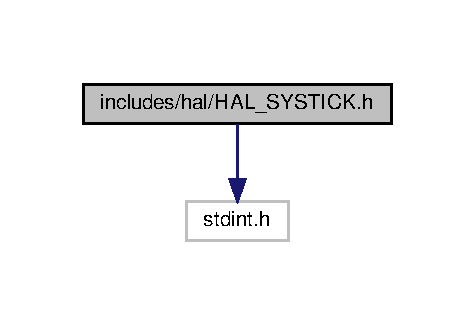
\includegraphics[width=228pt]{HAL__SYSTICK_8h__incl}
\end{center}
\end{figure}
\subsection*{Funciones}
\begin{DoxyCompactItemize}
\item 
void \hyperlink{HAL__SYSTICK_8h_a29eb17e59d26a3f1a1f9184154964f36}{hal\+\_\+systick\+\_\+init} (uint32\+\_\+t tick\+\_\+us, void($\ast$callback)(void))
\begin{DoxyCompactList}\small\item\em Inicializacion del S\+Y\+S\+T\+I\+CK. \end{DoxyCompactList}\item 
void \hyperlink{HAL__SYSTICK_8h_a7291cb0d9994e019d2b2e804f454b571}{hal\+\_\+systick\+\_\+update\+\_\+callback} (void($\ast$callback)(void))
\begin{DoxyCompactList}\small\item\em Actualizar callback del S\+Y\+S\+T\+I\+CK. \end{DoxyCompactList}\end{DoxyCompactItemize}


\subsection{Descripción detallada}
Declaraciones a nivel de aplicacion del periferico S\+Y\+S\+I\+CK (L\+P\+C845) 

\begin{DoxyAuthor}{Autor}
Augusto Santini 
\end{DoxyAuthor}
\begin{DoxyDate}{Fecha}
3/2020 
\end{DoxyDate}
\begin{DoxyVersion}{Versión}
1.\+0 
\end{DoxyVersion}


\subsection{Documentación de las funciones}
\mbox{\Hypertarget{HAL__SYSTICK_8h_a29eb17e59d26a3f1a1f9184154964f36}\label{HAL__SYSTICK_8h_a29eb17e59d26a3f1a1f9184154964f36}} 
\index{H\+A\+L\+\_\+\+S\+Y\+S\+T\+I\+C\+K.\+h@{H\+A\+L\+\_\+\+S\+Y\+S\+T\+I\+C\+K.\+h}!hal\+\_\+systick\+\_\+init@{hal\+\_\+systick\+\_\+init}}
\index{hal\+\_\+systick\+\_\+init@{hal\+\_\+systick\+\_\+init}!H\+A\+L\+\_\+\+S\+Y\+S\+T\+I\+C\+K.\+h@{H\+A\+L\+\_\+\+S\+Y\+S\+T\+I\+C\+K.\+h}}
\subsubsection{\texorpdfstring{hal\+\_\+systick\+\_\+init()}{hal\_systick\_init()}}
{\footnotesize\ttfamily void hal\+\_\+systick\+\_\+init (\begin{DoxyParamCaption}\item[{uint32\+\_\+t}]{tick\+\_\+us,  }\item[{void($\ast$)(void)}]{callback }\end{DoxyParamCaption})}



Inicializacion del S\+Y\+S\+T\+I\+CK. 


\begin{DoxyParams}[1]{Parámetros}
\mbox{\tt in}  & {\em tick\+\_\+us} & Tiempo en microsegundos deseado para el tick \\
\hline
\mbox{\tt in}  & {\em callback} & Funcion a llamar en cada tick \\
\hline
\end{DoxyParams}
\begin{Desc}
\item[Ejemplos\+: ]\par
\hyperlink{Ejemplo_ADC_8c-example}{Ejemplo\+\_\+\+A\+D\+C.\+c}.\end{Desc}
\mbox{\Hypertarget{HAL__SYSTICK_8h_a7291cb0d9994e019d2b2e804f454b571}\label{HAL__SYSTICK_8h_a7291cb0d9994e019d2b2e804f454b571}} 
\index{H\+A\+L\+\_\+\+S\+Y\+S\+T\+I\+C\+K.\+h@{H\+A\+L\+\_\+\+S\+Y\+S\+T\+I\+C\+K.\+h}!hal\+\_\+systick\+\_\+update\+\_\+callback@{hal\+\_\+systick\+\_\+update\+\_\+callback}}
\index{hal\+\_\+systick\+\_\+update\+\_\+callback@{hal\+\_\+systick\+\_\+update\+\_\+callback}!H\+A\+L\+\_\+\+S\+Y\+S\+T\+I\+C\+K.\+h@{H\+A\+L\+\_\+\+S\+Y\+S\+T\+I\+C\+K.\+h}}
\subsubsection{\texorpdfstring{hal\+\_\+systick\+\_\+update\+\_\+callback()}{hal\_systick\_update\_callback()}}
{\footnotesize\ttfamily void hal\+\_\+systick\+\_\+update\+\_\+callback (\begin{DoxyParamCaption}\item[{void($\ast$)(void)}]{callback }\end{DoxyParamCaption})}



Actualizar callback del S\+Y\+S\+T\+I\+CK. 


\begin{DoxyParams}[1]{Parámetros}
\mbox{\tt in}  & {\em callback} & Nuevo callback a ejecutar en cada tick \\
\hline
\end{DoxyParams}

\hypertarget{HAL__UART_8h}{}\doxysection{Referencia del Archivo includes/hal/\+H\+A\+L\+\_\+\+U\+A\+RT.h}
\label{HAL__UART_8h}\index{includes/hal/HAL\_UART.h@{includes/hal/HAL\_UART.h}}


Declaraciones a nivel de aplicacion del periferico U\+A\+RT (L\+P\+C845)  


{\ttfamily \#include $<$stdint.\+h$>$}\newline
{\ttfamily \#include $<$H\+A\+L\+\_\+\+S\+Y\+S\+C\+O\+N.\+h$>$}\newline
{\ttfamily \#include $<$H\+A\+L\+\_\+\+G\+P\+I\+O.\+h$>$}\newline
Dependencia gráfica adjunta para H\+A\+L\+\_\+\+U\+A\+R\+T.\+h\+:\nopagebreak
\begin{figure}[H]
\begin{center}
\leavevmode
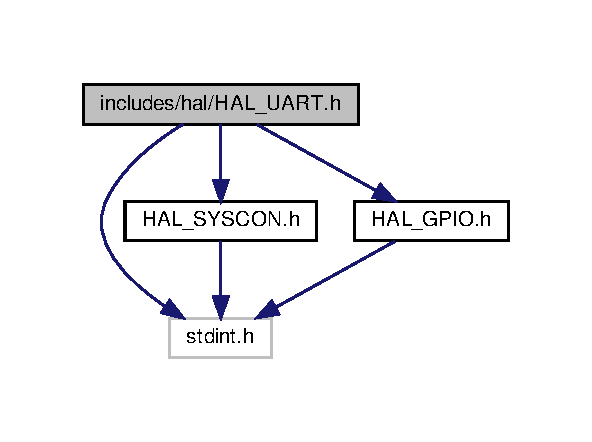
\includegraphics[width=284pt]{HAL__UART_8h__incl}
\end{center}
\end{figure}
\doxysubsection*{Estructuras de datos}
\begin{DoxyCompactItemize}
\item 
struct \mbox{\hyperlink{structhal__uart__config__t}{hal\+\_\+uart\+\_\+config\+\_\+t}}
\end{DoxyCompactItemize}
\doxysubsection*{Enumeraciones}
\begin{DoxyCompactItemize}
\item 
\mbox{\Hypertarget{HAL__UART_8h_a7eb9eb1e60b93c109e14ac618ab7901e}\label{HAL__UART_8h_a7eb9eb1e60b93c109e14ac618ab7901e}} 
enum {\bfseries hal\+\_\+uart\+\_\+datalen\+\_\+en} \{ {\bfseries H\+A\+L\+\_\+\+U\+A\+R\+T\+\_\+\+D\+A\+T\+A\+L\+E\+N\+\_\+7\+B\+IT} = 0, 
{\bfseries H\+A\+L\+\_\+\+U\+A\+R\+T\+\_\+\+D\+A\+T\+A\+L\+E\+N\+\_\+8\+B\+IT}, 
{\bfseries H\+A\+L\+\_\+\+U\+A\+R\+T\+\_\+\+D\+A\+T\+A\+L\+E\+N\+\_\+9\+B\+IT}
 \}
\item 
\mbox{\Hypertarget{HAL__UART_8h_a220ffe3b05d04a08e12a6193549511d1}\label{HAL__UART_8h_a220ffe3b05d04a08e12a6193549511d1}} 
enum {\bfseries hal\+\_\+uart\+\_\+parity\+\_\+en} \{ {\bfseries H\+A\+L\+\_\+\+U\+A\+R\+T\+\_\+\+P\+A\+R\+I\+T\+Y\+\_\+\+N\+O\+\_\+\+P\+A\+R\+I\+TY} = 0, 
{\bfseries H\+A\+L\+\_\+\+U\+A\+R\+T\+\_\+\+P\+A\+R\+I\+T\+Y\+\_\+\+E\+V\+EN} = 2, 
{\bfseries H\+A\+L\+\_\+\+U\+A\+R\+T\+\_\+\+P\+A\+R\+I\+T\+Y\+\_\+\+O\+DD}
 \}
\item 
\mbox{\Hypertarget{HAL__UART_8h_a55a5b3c508317c2fdbc41525d7c8bc97}\label{HAL__UART_8h_a55a5b3c508317c2fdbc41525d7c8bc97}} 
enum {\bfseries hal\+\_\+uart\+\_\+stop\+\_\+en} \{ {\bfseries H\+A\+L\+\_\+\+U\+A\+R\+T\+\_\+\+S\+T\+O\+P\+L\+E\+N\+\_\+1\+B\+IT} = 0, 
{\bfseries H\+A\+L\+\_\+\+U\+A\+R\+T\+\_\+\+S\+T\+O\+P\+L\+E\+N\+\_\+2\+B\+IT}
 \}
\item 
\mbox{\Hypertarget{HAL__UART_8h_a43bd29e1a1f8591ef801d070f55afc93}\label{HAL__UART_8h_a43bd29e1a1f8591ef801d070f55afc93}} 
enum {\bfseries hal\+\_\+uart\+\_\+oversampling\+\_\+en} \{ \newline
{\bfseries H\+A\+L\+\_\+\+U\+A\+R\+T\+\_\+\+O\+V\+E\+R\+S\+A\+M\+P\+L\+I\+N\+G\+\_\+\+X5} = 4, 
{\bfseries H\+A\+L\+\_\+\+U\+A\+R\+T\+\_\+\+O\+V\+E\+R\+S\+A\+M\+P\+L\+I\+N\+G\+\_\+\+X6}, 
{\bfseries H\+A\+L\+\_\+\+U\+A\+R\+T\+\_\+\+O\+V\+E\+R\+S\+A\+M\+P\+L\+I\+N\+G\+\_\+\+X7}, 
{\bfseries H\+A\+L\+\_\+\+U\+A\+R\+T\+\_\+\+O\+V\+E\+R\+S\+A\+M\+P\+L\+I\+N\+G\+\_\+\+X8}, 
\newline
{\bfseries H\+A\+L\+\_\+\+U\+A\+R\+T\+\_\+\+O\+V\+E\+R\+S\+A\+M\+P\+L\+I\+N\+G\+\_\+\+X9}, 
{\bfseries H\+A\+L\+\_\+\+U\+A\+R\+T\+\_\+\+O\+V\+E\+R\+S\+A\+M\+P\+L\+I\+N\+G\+\_\+\+X10}, 
{\bfseries H\+A\+L\+\_\+\+U\+A\+R\+T\+\_\+\+O\+V\+E\+R\+S\+A\+M\+P\+L\+I\+N\+G\+\_\+\+X11}, 
{\bfseries H\+A\+L\+\_\+\+U\+A\+R\+T\+\_\+\+O\+V\+E\+R\+S\+A\+M\+P\+L\+I\+N\+G\+\_\+\+X12}, 
\newline
{\bfseries H\+A\+L\+\_\+\+U\+A\+R\+T\+\_\+\+O\+V\+E\+R\+S\+A\+M\+P\+L\+I\+N\+G\+\_\+\+X13}, 
{\bfseries H\+A\+L\+\_\+\+U\+A\+R\+T\+\_\+\+O\+V\+E\+R\+S\+A\+M\+P\+L\+I\+N\+G\+\_\+\+X14}, 
{\bfseries H\+A\+L\+\_\+\+U\+A\+R\+T\+\_\+\+O\+V\+E\+R\+S\+A\+M\+P\+L\+I\+N\+G\+\_\+\+X15}, 
{\bfseries H\+A\+L\+\_\+\+U\+A\+R\+T\+\_\+\+O\+V\+E\+R\+S\+A\+M\+P\+L\+I\+N\+G\+\_\+\+X16}
 \}
\item 
\mbox{\Hypertarget{HAL__UART_8h_a901ade8c04909ed853a3e232aaecff10}\label{HAL__UART_8h_a901ade8c04909ed853a3e232aaecff10}} 
enum {\bfseries hal\+\_\+uart\+\_\+tx\+\_\+result} \{ {\bfseries H\+A\+L\+\_\+\+U\+A\+R\+T\+\_\+\+T\+X\+\_\+\+R\+E\+S\+U\+L\+T\+\_\+\+OK} = 0, 
{\bfseries H\+A\+L\+\_\+\+U\+A\+R\+T\+\_\+\+T\+X\+\_\+\+R\+E\+S\+U\+L\+T\+\_\+\+N\+O\+T\+\_\+\+R\+E\+A\+DY}
 \}
\item 
\mbox{\Hypertarget{HAL__UART_8h_a165cd0258bebd3dbfaaeb878b3e4a611}\label{HAL__UART_8h_a165cd0258bebd3dbfaaeb878b3e4a611}} 
enum {\bfseries hal\+\_\+uart\+\_\+rx\+\_\+result} \{ {\bfseries H\+A\+L\+\_\+\+U\+A\+R\+T\+\_\+\+R\+X\+\_\+\+R\+E\+S\+U\+L\+T\+\_\+\+OK} = 0, 
{\bfseries H\+A\+L\+\_\+\+U\+A\+R\+T\+\_\+\+R\+X\+\_\+\+R\+E\+S\+U\+L\+T\+\_\+\+N\+O\+T\+\_\+\+R\+E\+A\+DY}
 \}
\end{DoxyCompactItemize}
\doxysubsection*{Funciones}
\begin{DoxyCompactItemize}
\item 
void \mbox{\hyperlink{HAL__UART_8h_ae847e2762fdcf69766487fbea2eed69a}{hal\+\_\+uart\+\_\+init}} (uint8\+\_\+t inst, const \mbox{\hyperlink{structhal__uart__config__t}{hal\+\_\+uart\+\_\+config\+\_\+t}} $\ast$config)
\begin{DoxyCompactList}\small\item\em Inicializar U\+A\+RT con los parametros deseados. \end{DoxyCompactList}\item 
hal\+\_\+uart\+\_\+tx\+\_\+result \mbox{\hyperlink{HAL__UART_8h_aac3ebe57d6954db26baedbafdc64fb26}{hal\+\_\+uart\+\_\+tx\+\_\+byte}} (uint8\+\_\+t inst, uint32\+\_\+t data)
\begin{DoxyCompactList}\small\item\em Transmitir un dato mediante la U\+A\+RT. \end{DoxyCompactList}\item 
hal\+\_\+uart\+\_\+rx\+\_\+result \mbox{\hyperlink{HAL__UART_8h_aa9186f2bbb7ce6c298e4e6249341a99a}{hal\+\_\+uart\+\_\+rx\+\_\+byte}} (uint8\+\_\+t inst, uint32\+\_\+t $\ast$data)
\begin{DoxyCompactList}\small\item\em Recibir un dato de la U\+A\+RT. \end{DoxyCompactList}\item 
void \mbox{\hyperlink{HAL__UART_8h_a014876b7037b10d418c3b2006f894f1e}{hal\+\_\+uart\+\_\+register\+\_\+tx\+\_\+callback}} (uint8\+\_\+t inst, void($\ast$new\+\_\+callback)(void))
\begin{DoxyCompactList}\small\item\em Registrar el callback a ser llamado una vez finalizada la transmision de un dato por U\+A\+RT. \end{DoxyCompactList}\item 
void \mbox{\hyperlink{HAL__UART_8h_a07491f4d61942f763b49526e81e2a35d}{hal\+\_\+uart\+\_\+register\+\_\+rx\+\_\+callback}} (uint8\+\_\+t inst, void($\ast$new\+\_\+callback)(void))
\begin{DoxyCompactList}\small\item\em Registrar el callback a ser llamado en la recepcion de un dato por U\+A\+RT. \end{DoxyCompactList}\item 
\mbox{\Hypertarget{HAL__UART_8h_a7a61d73fd6ad0a670c4225140fefd7bd}\label{HAL__UART_8h_a7a61d73fd6ad0a670c4225140fefd7bd}} 
void \mbox{\hyperlink{HAL__UART_8h_a7a61d73fd6ad0a670c4225140fefd7bd}{U\+A\+R\+T3\+\_\+irq}} (void)
\begin{DoxyCompactList}\small\item\em Interrupcion de U\+A\+R\+T3. \end{DoxyCompactList}\item 
\mbox{\Hypertarget{HAL__UART_8h_a28aab3f4a90a2a9d61d88048637c0811}\label{HAL__UART_8h_a28aab3f4a90a2a9d61d88048637c0811}} 
void \mbox{\hyperlink{HAL__UART_8h_a28aab3f4a90a2a9d61d88048637c0811}{U\+A\+R\+T4\+\_\+irq}} (void)
\begin{DoxyCompactList}\small\item\em Interrupcion de U\+A\+R\+T4. \end{DoxyCompactList}\end{DoxyCompactItemize}


\doxysubsection{Descripción detallada}
Declaraciones a nivel de aplicacion del periferico U\+A\+RT (L\+P\+C845) 

\begin{DoxyAuthor}{Autor}
Augusto Santini 
\end{DoxyAuthor}
\begin{DoxyDate}{Fecha}
3/2020 
\end{DoxyDate}
\begin{DoxyVersion}{Versión}
1.\+0 
\end{DoxyVersion}


\doxysubsection{Documentación de las funciones}
\mbox{\Hypertarget{HAL__UART_8h_ae847e2762fdcf69766487fbea2eed69a}\label{HAL__UART_8h_ae847e2762fdcf69766487fbea2eed69a}} 
\index{HAL\_UART.h@{HAL\_UART.h}!hal\_uart\_init@{hal\_uart\_init}}
\index{hal\_uart\_init@{hal\_uart\_init}!HAL\_UART.h@{HAL\_UART.h}}
\doxysubsubsection{\texorpdfstring{hal\_uart\_init()}{hal\_uart\_init()}}
{\footnotesize\ttfamily void hal\+\_\+uart\+\_\+init (\begin{DoxyParamCaption}\item[{uint8\+\_\+t}]{inst,  }\item[{const \mbox{\hyperlink{structhal__uart__config__t}{hal\+\_\+uart\+\_\+config\+\_\+t}} $\ast$}]{config }\end{DoxyParamCaption})}



Inicializar U\+A\+RT con los parametros deseados. 


\begin{DoxyParams}[1]{Parámetros}
\mbox{\texttt{ in}}  & {\em inst} & Que instancia de U\+A\+RT inicializar \\
\hline
\mbox{\texttt{ in}}  & {\em config} & Puntero a configuracion de la U\+A\+RT \\
\hline
\end{DoxyParams}
\mbox{\Hypertarget{HAL__UART_8h_aac3ebe57d6954db26baedbafdc64fb26}\label{HAL__UART_8h_aac3ebe57d6954db26baedbafdc64fb26}} 
\index{HAL\_UART.h@{HAL\_UART.h}!hal\_uart\_tx\_byte@{hal\_uart\_tx\_byte}}
\index{hal\_uart\_tx\_byte@{hal\_uart\_tx\_byte}!HAL\_UART.h@{HAL\_UART.h}}
\doxysubsubsection{\texorpdfstring{hal\_uart\_tx\_byte()}{hal\_uart\_tx\_byte()}}
{\footnotesize\ttfamily hal\+\_\+uart\+\_\+tx\+\_\+result hal\+\_\+uart\+\_\+tx\+\_\+byte (\begin{DoxyParamCaption}\item[{uint8\+\_\+t}]{inst,  }\item[{uint32\+\_\+t}]{data }\end{DoxyParamCaption})}



Transmitir un dato mediante la U\+A\+RT. 


\begin{DoxyParams}[1]{Parámetros}
\mbox{\texttt{ in}}  & {\em inst} & Que instancia de U\+A\+RT usar \\
\hline
\mbox{\texttt{ in}}  & {\em data} & Dato a transmitir. Puede ser de 7, 8 o 9 bits \\
\hline
\end{DoxyParams}
\mbox{\Hypertarget{HAL__UART_8h_aa9186f2bbb7ce6c298e4e6249341a99a}\label{HAL__UART_8h_aa9186f2bbb7ce6c298e4e6249341a99a}} 
\index{HAL\_UART.h@{HAL\_UART.h}!hal\_uart\_rx\_byte@{hal\_uart\_rx\_byte}}
\index{hal\_uart\_rx\_byte@{hal\_uart\_rx\_byte}!HAL\_UART.h@{HAL\_UART.h}}
\doxysubsubsection{\texorpdfstring{hal\_uart\_rx\_byte()}{hal\_uart\_rx\_byte()}}
{\footnotesize\ttfamily hal\+\_\+uart\+\_\+rx\+\_\+result hal\+\_\+uart\+\_\+rx\+\_\+byte (\begin{DoxyParamCaption}\item[{uint8\+\_\+t}]{inst,  }\item[{uint32\+\_\+t $\ast$}]{data }\end{DoxyParamCaption})}



Recibir un dato de la U\+A\+RT. 


\begin{DoxyParams}[1]{Parámetros}
\mbox{\texttt{ in}}  & {\em inst} & Que instancia de U\+A\+RT usar \\
\hline
\mbox{\texttt{ in}}  & {\em data} & Puntero a donde guardar el dato recibido \\
\hline
\end{DoxyParams}
\begin{DoxyReturn}{Devuelve}
Estado de la recepcion 
\end{DoxyReturn}
\mbox{\Hypertarget{HAL__UART_8h_a014876b7037b10d418c3b2006f894f1e}\label{HAL__UART_8h_a014876b7037b10d418c3b2006f894f1e}} 
\index{HAL\_UART.h@{HAL\_UART.h}!hal\_uart\_register\_tx\_callback@{hal\_uart\_register\_tx\_callback}}
\index{hal\_uart\_register\_tx\_callback@{hal\_uart\_register\_tx\_callback}!HAL\_UART.h@{HAL\_UART.h}}
\doxysubsubsection{\texorpdfstring{hal\_uart\_register\_tx\_callback()}{hal\_uart\_register\_tx\_callback()}}
{\footnotesize\ttfamily void hal\+\_\+uart\+\_\+register\+\_\+tx\+\_\+callback (\begin{DoxyParamCaption}\item[{uint8\+\_\+t}]{inst,  }\item[{void($\ast$)(void)}]{new\+\_\+callback }\end{DoxyParamCaption})}



Registrar el callback a ser llamado una vez finalizada la transmision de un dato por U\+A\+RT. 


\begin{DoxyParams}[1]{Parámetros}
\mbox{\texttt{ in}}  & {\em inst} & A que instancia de U\+A\+RT registrar el callback \\
\hline
\mbox{\texttt{ in}}  & {\em new\+\_\+callback} & Puntero a funcion a llamar cada vez que se termina de enviar un dato por U\+A\+RT \\
\hline
\end{DoxyParams}
\mbox{\Hypertarget{HAL__UART_8h_a07491f4d61942f763b49526e81e2a35d}\label{HAL__UART_8h_a07491f4d61942f763b49526e81e2a35d}} 
\index{HAL\_UART.h@{HAL\_UART.h}!hal\_uart\_register\_rx\_callback@{hal\_uart\_register\_rx\_callback}}
\index{hal\_uart\_register\_rx\_callback@{hal\_uart\_register\_rx\_callback}!HAL\_UART.h@{HAL\_UART.h}}
\doxysubsubsection{\texorpdfstring{hal\_uart\_register\_rx\_callback()}{hal\_uart\_register\_rx\_callback()}}
{\footnotesize\ttfamily void hal\+\_\+uart\+\_\+register\+\_\+rx\+\_\+callback (\begin{DoxyParamCaption}\item[{uint8\+\_\+t}]{inst,  }\item[{void($\ast$)(void)}]{new\+\_\+callback }\end{DoxyParamCaption})}



Registrar el callback a ser llamado en la recepcion de un dato por U\+A\+RT. 


\begin{DoxyParams}[1]{Parámetros}
\mbox{\texttt{ in}}  & {\em inst} & A que instancia de U\+A\+RT registrar el callback \\
\hline
\mbox{\texttt{ in}}  & {\em new\+\_\+callback} & Puntero a funcion a llamar cada vez que se recibe un dato por U\+A\+RT \\
\hline
\end{DoxyParams}

\hypertarget{HAL__WKT_8h}{}\section{Referencia del Archivo includes/hal/\+H\+A\+L\+\_\+\+W\+KT.h}
\label{HAL__WKT_8h}\index{includes/hal/\+H\+A\+L\+\_\+\+W\+K\+T.\+h@{includes/hal/\+H\+A\+L\+\_\+\+W\+K\+T.\+h}}


Declaraciones a nivel de aplicacion del periferico W\+KT (L\+P\+C845)  


{\ttfamily \#include $<$stdint.\+h$>$}\newline
Dependencia gráfica adjunta para H\+A\+L\+\_\+\+W\+K\+T.\+h\+:
\nopagebreak
\begin{figure}[H]
\begin{center}
\leavevmode
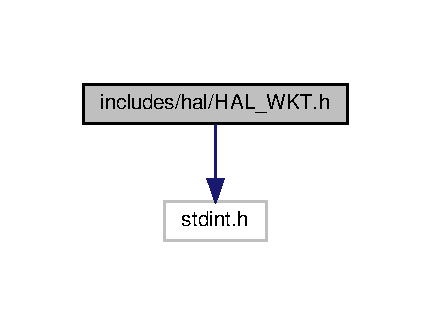
\includegraphics[width=207pt]{HAL__WKT_8h__incl}
\end{center}
\end{figure}
\subsection*{Enumeraciones}
\begin{DoxyCompactItemize}
\item 
\mbox{\Hypertarget{HAL__WKT_8h_afe3a7131eaa16754febfe27e0da02823}\label{HAL__WKT_8h_afe3a7131eaa16754febfe27e0da02823}} 
enum {\bfseries hal\+\_\+wkt\+\_\+clock\+\_\+source\+\_\+en} \{ {\bfseries H\+A\+L\+\_\+\+W\+K\+T\+\_\+\+C\+L\+O\+C\+K\+\_\+\+S\+O\+U\+R\+C\+E\+\_\+\+F\+R\+O\+\_\+\+D\+IV} = 0, 
{\bfseries H\+A\+L\+\_\+\+W\+K\+T\+\_\+\+C\+L\+O\+C\+K\+\_\+\+S\+O\+U\+R\+C\+E\+\_\+\+L\+O\+W\+\_\+\+P\+O\+W\+E\+R\+\_\+\+O\+SC}, 
{\bfseries H\+A\+L\+\_\+\+W\+K\+T\+\_\+\+C\+L\+O\+C\+K\+\_\+\+S\+O\+U\+R\+C\+E\+\_\+\+E\+X\+T\+E\+R\+N\+AL}
 \}
\end{DoxyCompactItemize}
\subsection*{Funciones}
\begin{DoxyCompactItemize}
\item 
void \hyperlink{HAL__WKT_8h_aeb732cadeaab8af681865670e8beab43}{hal\+\_\+wkt\+\_\+init} (hal\+\_\+wkt\+\_\+clock\+\_\+source\+\_\+en clock\+\_\+sel, uint32\+\_\+t ext\+\_\+clock\+\_\+value, void($\ast$callback)(void))
\begin{DoxyCompactList}\small\item\em Inicializar el W\+KT. \end{DoxyCompactList}\item 
\mbox{\Hypertarget{HAL__WKT_8h_a985343b8388f0830ebc106d298520d49}\label{HAL__WKT_8h_a985343b8388f0830ebc106d298520d49}} 
void {\bfseries hal\+\_\+wkt\+\_\+select\+\_\+clock\+\_\+source} (hal\+\_\+wkt\+\_\+clock\+\_\+source\+\_\+en clock\+\_\+sel, uint32\+\_\+t ext\+\_\+clock\+\_\+value)
\item 
void \hyperlink{HAL__WKT_8h_a83ba94b350eac43185f64f92e6a2ceab}{hal\+\_\+wkt\+\_\+register\+\_\+callback} (void($\ast$new\+\_\+callback)(void))
\begin{DoxyCompactList}\small\item\em Registrar un callback para la interrupcion del W\+KT. \end{DoxyCompactList}\item 
\mbox{\Hypertarget{HAL__WKT_8h_ab12f0980a1cf6c8338ea5df990ec2d13}\label{HAL__WKT_8h_ab12f0980a1cf6c8338ea5df990ec2d13}} 
void {\bfseries hal\+\_\+wkt\+\_\+start\+\_\+count} (uint32\+\_\+t time\+\_\+useg)
\item 
\mbox{\Hypertarget{HAL__WKT_8h_a1c617a5813b80a65229c86f810ae0c3b}\label{HAL__WKT_8h_a1c617a5813b80a65229c86f810ae0c3b}} 
void {\bfseries hal\+\_\+wkt\+\_\+start\+\_\+count\+\_\+with\+\_\+value} (uint32\+\_\+t value)
\end{DoxyCompactItemize}


\subsection{Descripción detallada}
Declaraciones a nivel de aplicacion del periferico W\+KT (L\+P\+C845) 

\begin{DoxyAuthor}{Autor}
Augusto Santini 
\end{DoxyAuthor}
\begin{DoxyDate}{Fecha}
3/2020 
\end{DoxyDate}
\begin{DoxyVersion}{Versión}
1.\+0 
\end{DoxyVersion}


\subsection{Documentación de las funciones}
\mbox{\Hypertarget{HAL__WKT_8h_aeb732cadeaab8af681865670e8beab43}\label{HAL__WKT_8h_aeb732cadeaab8af681865670e8beab43}} 
\index{H\+A\+L\+\_\+\+W\+K\+T.\+h@{H\+A\+L\+\_\+\+W\+K\+T.\+h}!hal\+\_\+wkt\+\_\+init@{hal\+\_\+wkt\+\_\+init}}
\index{hal\+\_\+wkt\+\_\+init@{hal\+\_\+wkt\+\_\+init}!H\+A\+L\+\_\+\+W\+K\+T.\+h@{H\+A\+L\+\_\+\+W\+K\+T.\+h}}
\subsubsection{\texorpdfstring{hal\+\_\+wkt\+\_\+init()}{hal\_wkt\_init()}}
{\footnotesize\ttfamily void hal\+\_\+wkt\+\_\+init (\begin{DoxyParamCaption}\item[{hal\+\_\+wkt\+\_\+clock\+\_\+source\+\_\+en}]{clock\+\_\+sel,  }\item[{uint32\+\_\+t}]{ext\+\_\+clock\+\_\+value,  }\item[{void($\ast$)(void)}]{callback }\end{DoxyParamCaption})}



Inicializar el W\+KT. 


\begin{DoxyParams}[1]{Parámetros}
\mbox{\tt in}  & {\em clock\+\_\+sel} & Seleccion de clock deseada para el W\+KT \\
\hline
\mbox{\tt in}  & {\em ext\+\_\+clock\+\_\+value} & Valor de clock externo (si la seleccion es interna, no importa este parametro) \\
\hline
\mbox{\tt in}  & {\em callback} & Callback a ejecutar en la interrupcion del W\+KT \\
\hline
\end{DoxyParams}
\mbox{\Hypertarget{HAL__WKT_8h_a83ba94b350eac43185f64f92e6a2ceab}\label{HAL__WKT_8h_a83ba94b350eac43185f64f92e6a2ceab}} 
\index{H\+A\+L\+\_\+\+W\+K\+T.\+h@{H\+A\+L\+\_\+\+W\+K\+T.\+h}!hal\+\_\+wkt\+\_\+register\+\_\+callback@{hal\+\_\+wkt\+\_\+register\+\_\+callback}}
\index{hal\+\_\+wkt\+\_\+register\+\_\+callback@{hal\+\_\+wkt\+\_\+register\+\_\+callback}!H\+A\+L\+\_\+\+W\+K\+T.\+h@{H\+A\+L\+\_\+\+W\+K\+T.\+h}}
\subsubsection{\texorpdfstring{hal\+\_\+wkt\+\_\+register\+\_\+callback()}{hal\_wkt\_register\_callback()}}
{\footnotesize\ttfamily void hal\+\_\+wkt\+\_\+register\+\_\+callback (\begin{DoxyParamCaption}\item[{void($\ast$)(void)}]{new\+\_\+callback }\end{DoxyParamCaption})}



Registrar un callback para la interrupcion del W\+KT. 


\begin{DoxyParams}[1]{Parámetros}
\mbox{\tt in}  & {\em new\+\_\+callback} & Nuevo callback para la interrupcion del W\+KT \\
\hline
\end{DoxyParams}

\hypertarget{HPL__ADC_8h}{}\section{Referencia del Archivo includes/hpl/\+H\+P\+L\+\_\+\+A\+DC.h}
\label{HPL__ADC_8h}\index{includes/hpl/\+H\+P\+L\+\_\+\+A\+D\+C.\+h@{includes/hpl/\+H\+P\+L\+\_\+\+A\+D\+C.\+h}}


Declaraciones a nivel de abstraccion de periferico del A\+DC (L\+P\+C845)  


{\ttfamily \#include $<$H\+R\+I\+\_\+\+A\+D\+C.\+h$>$}\newline
Dependencia gráfica adjunta para H\+P\+L\+\_\+\+A\+D\+C.\+h\+:
\nopagebreak
\begin{figure}[H]
\begin{center}
\leavevmode
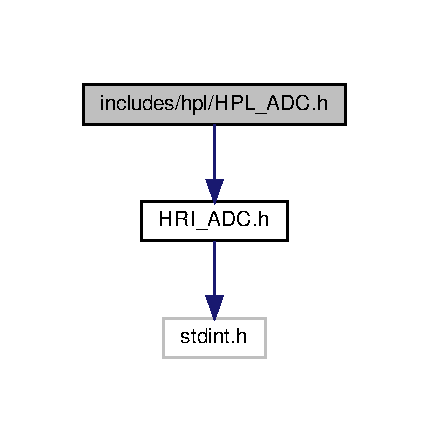
\includegraphics[width=206pt]{d1/d94/HPL__ADC_8h__incl}
\end{center}
\end{figure}
Gráfico de los archivos que directa o indirectamente incluyen a este archivo\+:\nopagebreak
\begin{figure}[H]
\begin{center}
\leavevmode
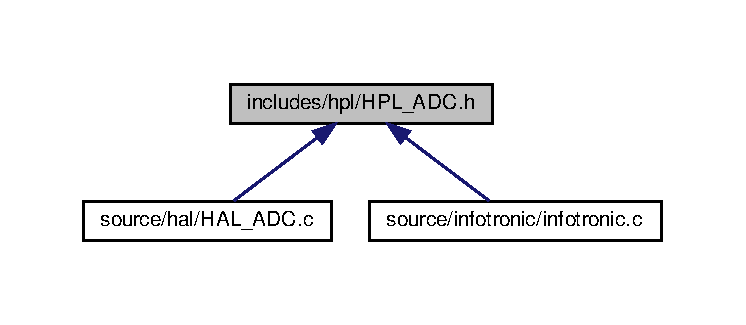
\includegraphics[width=350pt]{d0/d8d/HPL__ADC_8h__dep__incl}
\end{center}
\end{figure}
\subsection*{Estructuras de datos}
\begin{DoxyCompactItemize}
\item 
struct \hyperlink{HPL__ADC_8h_d8/d2c/structADC__global__data__t}{A\+D\+C\+\_\+global\+\_\+data\+\_\+t}
\item 
struct \hyperlink{HPL__ADC_8h_dd/dd6/structADC__channel__data__t}{A\+D\+C\+\_\+channel\+\_\+data\+\_\+t}
\end{DoxyCompactItemize}
\subsection*{Enumeraciones}
\begin{DoxyCompactItemize}
\item 
\mbox{\Hypertarget{HPL__ADC_8h_a00ba32f1aa7a302714f67324f1debf18}\label{HPL__ADC_8h_a00ba32f1aa7a302714f67324f1debf18}} 
enum {\bfseries A\+D\+C\+\_\+sequence\+\_\+sel\+\_\+en} \{ {\bfseries A\+D\+C\+\_\+\+S\+E\+Q\+U\+E\+N\+C\+E\+\_\+\+S\+E\+L\+\_\+A} = 0, 
{\bfseries A\+D\+C\+\_\+\+S\+E\+Q\+U\+E\+N\+C\+E\+\_\+\+S\+E\+L\+\_\+B}
 \}
\item 
\mbox{\Hypertarget{HPL__ADC_8h_ab21589108767870dc4eb185316681091}\label{HPL__ADC_8h_ab21589108767870dc4eb185316681091}} 
enum {\bfseries A\+D\+C\+\_\+operation\+\_\+mode\+\_\+en} \{ {\bfseries A\+D\+C\+\_\+\+O\+P\+E\+R\+A\+T\+I\+O\+N\+\_\+\+M\+O\+D\+E\+\_\+\+S\+Y\+N\+C\+H\+R\+O\+N\+O\+US} = 0, 
{\bfseries A\+D\+C\+\_\+\+O\+P\+E\+R\+A\+T\+I\+O\+N\+\_\+\+M\+O\+D\+E\+\_\+\+A\+S\+Y\+N\+C\+H\+R\+O\+N\+O\+US}
 \}
\item 
\mbox{\Hypertarget{HPL__ADC_8h_a1731e86f61a94ef27562f6e66f60ce26}\label{HPL__ADC_8h_a1731e86f61a94ef27562f6e66f60ce26}} 
enum {\bfseries A\+D\+C\+\_\+low\+\_\+power\+\_\+mode\+\_\+en} \{ {\bfseries A\+D\+C\+\_\+\+L\+O\+W\+\_\+\+P\+O\+W\+E\+R\+\_\+\+M\+O\+D\+E\+\_\+\+D\+I\+S\+A\+B\+L\+ED} = 0, 
{\bfseries A\+D\+C\+\_\+\+L\+O\+W\+\_\+\+P\+O\+W\+E\+R\+\_\+\+M\+O\+D\+E\+\_\+\+E\+N\+A\+B\+L\+ED}
 \}
\item 
\mbox{\Hypertarget{HPL__ADC_8h_a662858cc3be775892471d2ca73428e0d}\label{HPL__ADC_8h_a662858cc3be775892471d2ca73428e0d}} 
enum {\bfseries A\+D\+C\+\_\+trigger\+\_\+sel\+\_\+en} \{ \newline
{\bfseries A\+D\+C\+\_\+\+T\+R\+I\+G\+G\+E\+R\+\_\+\+S\+E\+L\+\_\+\+N\+O\+NE} = 0, 
{\bfseries A\+D\+C\+\_\+\+T\+R\+I\+G\+G\+E\+R\+\_\+\+S\+E\+L\+\_\+\+P\+I\+N\+I\+N\+T0\+\_\+\+I\+RQ}, 
{\bfseries A\+D\+C\+\_\+\+T\+R\+I\+G\+G\+E\+R\+\_\+\+S\+E\+L\+\_\+\+P\+I\+N\+I\+N\+T1\+\_\+\+I\+RQ}, 
{\bfseries A\+D\+C\+\_\+\+T\+R\+I\+G\+G\+E\+R\+\_\+\+S\+E\+L\+\_\+\+S\+C\+T0\+\_\+\+O\+U\+T3}, 
\newline
{\bfseries A\+D\+C\+\_\+\+T\+R\+I\+G\+G\+E\+R\+\_\+\+S\+E\+L\+\_\+\+S\+C\+T0\+\_\+\+O\+U\+T4}, 
{\bfseries A\+D\+C\+\_\+\+T\+R\+I\+G\+G\+E\+R\+\_\+\+S\+E\+L\+\_\+\+T0\+\_\+\+M\+A\+T3}, 
{\bfseries A\+D\+C\+\_\+\+T\+R\+I\+G\+G\+E\+R\+\_\+\+S\+E\+L\+\_\+\+C\+M\+P0\+\_\+\+O\+U\+T\+\_\+\+A\+DC}, 
{\bfseries A\+D\+C\+\_\+\+T\+R\+I\+G\+G\+E\+R\+\_\+\+S\+E\+L\+\_\+\+G\+P\+I\+O\+\_\+\+I\+N\+T\+\_\+\+B\+M\+AT}, 
\newline
{\bfseries A\+D\+C\+\_\+\+T\+R\+I\+G\+G\+E\+R\+\_\+\+S\+E\+L\+\_\+\+A\+R\+M\+\_\+\+T\+X\+EV}
 \}
\item 
\mbox{\Hypertarget{HPL__ADC_8h_a7d0c909ad610582ac96c96866b7193eb}\label{HPL__ADC_8h_a7d0c909ad610582ac96c96866b7193eb}} 
enum {\bfseries A\+D\+C\+\_\+trigger\+\_\+pol\+\_\+sel\+\_\+en} \{ {\bfseries A\+D\+C\+\_\+\+T\+R\+I\+G\+G\+E\+R\+\_\+\+P\+O\+L\+\_\+\+S\+E\+L\+\_\+\+N\+E\+G\+A\+T\+I\+V\+E\+\_\+\+E\+D\+GE} = 0, 
{\bfseries A\+D\+C\+\_\+\+T\+R\+I\+G\+G\+E\+R\+\_\+\+P\+O\+L\+\_\+\+S\+E\+L\+\_\+\+P\+O\+S\+I\+T\+I\+V\+E\+\_\+\+E\+D\+GE}
 \}
\item 
\mbox{\Hypertarget{HPL__ADC_8h_aac1bf6af7948a81c95143081b616279a}\label{HPL__ADC_8h_aac1bf6af7948a81c95143081b616279a}} 
enum {\bfseries A\+D\+C\+\_\+sync\+\_\+sel\+\_\+en} \{ {\bfseries A\+D\+C\+\_\+\+S\+Y\+N\+C\+\_\+\+S\+E\+L\+\_\+\+E\+N\+A\+B\+L\+E\+\_\+\+S\+Y\+NC} = 0, 
{\bfseries A\+D\+C\+\_\+\+S\+Y\+N\+C\+\_\+\+S\+E\+L\+\_\+\+B\+Y\+P\+A\+S\+S\+\_\+\+S\+Y\+NC}
 \}
\item 
\mbox{\Hypertarget{HPL__ADC_8h_a1b2d533a0938903eac4d1b2b093fc2e2}\label{HPL__ADC_8h_a1b2d533a0938903eac4d1b2b093fc2e2}} 
enum {\bfseries A\+D\+C\+\_\+clock\+\_\+source\+\_\+en} \{ {\bfseries A\+D\+C\+\_\+\+C\+L\+O\+C\+K\+\_\+\+S\+O\+U\+R\+C\+E\+\_\+\+F\+RO} = 0, 
{\bfseries A\+D\+C\+\_\+\+C\+L\+O\+C\+K\+\_\+\+S\+O\+U\+R\+C\+E\+\_\+\+P\+LL}
 \}
\item 
\mbox{\Hypertarget{HPL__ADC_8h_a7539c07e0b39410f0c6c81fad7ccc671}\label{HPL__ADC_8h_a7539c07e0b39410f0c6c81fad7ccc671}} 
enum {\bfseries A\+D\+C\+\_\+threshold\+\_\+sel\+\_\+en} \{ {\bfseries A\+D\+C\+\_\+\+T\+H\+R\+E\+S\+H\+O\+L\+D\+\_\+\+S\+E\+L\+\_\+0} = 0, 
{\bfseries A\+D\+C\+\_\+\+T\+H\+R\+E\+S\+H\+O\+L\+D\+\_\+\+S\+E\+L\+\_\+1}
 \}
\item 
\mbox{\Hypertarget{HPL__ADC_8h_a5c583dfdfe19856a56d143273c39bf5a}\label{HPL__ADC_8h_a5c583dfdfe19856a56d143273c39bf5a}} 
enum {\bfseries A\+D\+C\+\_\+interrupt\+\_\+mode\+\_\+en} \{ {\bfseries A\+D\+C\+\_\+\+I\+N\+T\+E\+R\+R\+U\+P\+T\+\_\+\+M\+O\+D\+E\+\_\+\+E\+OC} = 0, 
{\bfseries A\+D\+C\+\_\+\+I\+N\+T\+E\+R\+R\+U\+P\+T\+\_\+\+M\+O\+D\+E\+\_\+\+E\+OS}
 \}
\item 
\mbox{\Hypertarget{HPL__ADC_8h_a4a0eebd9bcb2d639500a76e286d1ed37}\label{HPL__ADC_8h_a4a0eebd9bcb2d639500a76e286d1ed37}} 
enum {\bfseries A\+D\+C\+\_\+threshold\+\_\+interrupt\+\_\+sel\+\_\+en} \{ {\bfseries A\+D\+C\+\_\+\+T\+H\+R\+E\+S\+H\+O\+L\+D\+\_\+\+I\+N\+T\+E\+R\+R\+U\+P\+T\+\_\+\+S\+E\+L\+\_\+\+O\+U\+T\+S\+I\+DE} = 1, 
{\bfseries A\+D\+C\+\_\+\+T\+H\+R\+E\+S\+H\+O\+L\+D\+\_\+\+I\+N\+T\+E\+R\+R\+U\+P\+T\+\_\+\+S\+E\+L\+\_\+\+C\+R\+O\+S\+S\+I\+NG}
 \}
\item 
\mbox{\Hypertarget{HPL__ADC_8h_ad2890355fdb5e4822e667c93717208b8}\label{HPL__ADC_8h_ad2890355fdb5e4822e667c93717208b8}} 
enum {\bfseries A\+D\+C\+\_\+vrange\+\_\+sel\+\_\+en} \{ {\bfseries A\+D\+C\+\_\+\+V\+R\+A\+N\+G\+E\+\_\+\+H\+I\+G\+H\+\_\+\+V\+O\+L\+T\+A\+GE} = 0, 
{\bfseries A\+D\+C\+\_\+\+V\+R\+A\+N\+G\+E\+\_\+\+L\+O\+W\+\_\+\+V\+O\+L\+T\+A\+GE}
 \}
\end{DoxyCompactItemize}
\subsection*{Funciones}
\begin{DoxyCompactItemize}
\item 
static void \hyperlink{HPL__ADC_8h_ab24094d357db84e562e43bf824fc729a}{A\+D\+C\+\_\+control\+\_\+config} (uint8\+\_\+t div, A\+D\+C\+\_\+operation\+\_\+mode\+\_\+en operation, A\+D\+C\+\_\+low\+\_\+power\+\_\+mode\+\_\+en power)
\begin{DoxyCompactList}\small\item\em Configuracion del registro de control del A\+DC. \end{DoxyCompactList}\item 
static void \hyperlink{HPL__ADC_8h_a5bd10e5f94ea00aec42b2defa70b99d3}{A\+D\+C\+\_\+sequence\+\_\+config\+\_\+channels} (A\+D\+C\+\_\+sequence\+\_\+sel\+\_\+en sequence, uint16\+\_\+t channels)
\begin{DoxyCompactList}\small\item\em Configuracion de canales habilitados en una secuencia. \end{DoxyCompactList}\item 
static uint16\+\_\+t \hyperlink{HPL__ADC_8h_a2d748808e448e5a38ae21a5460396329}{A\+D\+C\+\_\+sequence\+\_\+get\+\_\+channels} (A\+D\+C\+\_\+sequence\+\_\+sel\+\_\+en sequence)
\begin{DoxyCompactList}\small\item\em Obtener los canales configuados en la secuencia. \end{DoxyCompactList}\item 
static void \hyperlink{HPL__ADC_8h_a9e34b22664fd6353bf02f63a3a1d2e8f}{A\+D\+C\+\_\+sequence\+\_\+config\+\_\+trigger} (A\+D\+C\+\_\+sequence\+\_\+sel\+\_\+en sequence, A\+D\+C\+\_\+trigger\+\_\+sel\+\_\+en trigger)
\begin{DoxyCompactList}\small\item\em Configuracion de trigger en una secuencia. \end{DoxyCompactList}\item 
static void \hyperlink{HPL__ADC_8h_a1d7a8e03098fa6be24327b606422e76f}{A\+D\+C\+\_\+sequence\+\_\+config\+\_\+trigger\+\_\+pol} (A\+D\+C\+\_\+sequence\+\_\+sel\+\_\+en sequence, A\+D\+C\+\_\+trigger\+\_\+pol\+\_\+sel\+\_\+en pol)
\begin{DoxyCompactList}\small\item\em Configuracion de la polaridad del trigger en una secuencia. \end{DoxyCompactList}\item 
static void \hyperlink{HPL__ADC_8h_a20ef73fe9712291f6e93501cc18f17fc}{A\+D\+C\+\_\+sequence\+\_\+config\+\_\+sync} (A\+D\+C\+\_\+sequence\+\_\+sel\+\_\+en sequence, A\+D\+C\+\_\+sync\+\_\+sel\+\_\+en sync)
\begin{DoxyCompactList}\small\item\em Configuracion de la sincronizacion en una secuencia. \end{DoxyCompactList}\item 
static void \hyperlink{HPL__ADC_8h_a4ef125eab51dd46357acd54ac57e817e}{A\+D\+C\+\_\+sequence\+\_\+set\+\_\+start} (A\+D\+C\+\_\+sequence\+\_\+sel\+\_\+en sequence)
\begin{DoxyCompactList}\small\item\em Iniciar conversiones por software en una secuencia. \end{DoxyCompactList}\item 
static void \hyperlink{HPL__ADC_8h_a32cbfd500dd8c6daa9ea1e80f4af363e}{A\+D\+C\+\_\+sequence\+\_\+set\+\_\+burst} (A\+D\+C\+\_\+sequence\+\_\+sel\+\_\+en sequence)
\begin{DoxyCompactList}\small\item\em Iniciar conversiones en rafaga en una secuencia. \end{DoxyCompactList}\item 
static void \hyperlink{HPL__ADC_8h_a01d3167d81f527fc8e0cad1a576270af}{A\+D\+C\+\_\+sequence\+\_\+clear\+\_\+burst} (A\+D\+C\+\_\+sequence\+\_\+sel\+\_\+en sequence)
\begin{DoxyCompactList}\small\item\em Detener conversiones en rafaga en una secuencia. \end{DoxyCompactList}\item 
static void \hyperlink{HPL__ADC_8h_a3b513d17cc16f27aa5fe2d145f9934e6}{A\+D\+C\+\_\+sequence\+\_\+set\+\_\+singlestep} (A\+D\+C\+\_\+sequence\+\_\+sel\+\_\+en sequence)
\begin{DoxyCompactList}\small\item\em Fijar modo singlestep. \end{DoxyCompactList}\item 
static void \hyperlink{HPL__ADC_8h_ac14967725662ff5f3d3db72086ece29c}{A\+D\+C\+\_\+sequence\+\_\+clear\+\_\+singlestep} (A\+D\+C\+\_\+sequence\+\_\+sel\+\_\+en sequence)
\begin{DoxyCompactList}\small\item\em Limpiar modo singlestep. \end{DoxyCompactList}\item 
\mbox{\Hypertarget{HPL__ADC_8h_ae450f32fa863a87a91ccf60351daac06}\label{HPL__ADC_8h_ae450f32fa863a87a91ccf60351daac06}} 
static void \hyperlink{HPL__ADC_8h_ae450f32fa863a87a91ccf60351daac06}{A\+D\+C\+\_\+sequence\+\_\+\+A\+\_\+lowpriority\+\_\+set} (void)
\begin{DoxyCompactList}\small\item\em Fijar baja prioridad para la secuencia A. \end{DoxyCompactList}\item 
\mbox{\Hypertarget{HPL__ADC_8h_aecf6fef0ff0634e679ce1f5fb0c62d36}\label{HPL__ADC_8h_aecf6fef0ff0634e679ce1f5fb0c62d36}} 
static void \hyperlink{HPL__ADC_8h_aecf6fef0ff0634e679ce1f5fb0c62d36}{A\+D\+C\+\_\+sequence\+\_\+\+A\+\_\+lowpriority\+\_\+clear} (void)
\begin{DoxyCompactList}\small\item\em Fijar baja prioridad para la secuencia A. \end{DoxyCompactList}\item 
static void \hyperlink{HPL__ADC_8h_a80eb450b5275099b1bd103d825a8b9cb}{A\+D\+C\+\_\+sequence\+\_\+config\+\_\+interrupt\+\_\+mode} (A\+D\+C\+\_\+sequence\+\_\+sel\+\_\+en sequence, A\+D\+C\+\_\+interrupt\+\_\+mode\+\_\+en mode)
\begin{DoxyCompactList}\small\item\em Configurar modo de interrupcion para una secuencia. \end{DoxyCompactList}\item 
static A\+D\+C\+\_\+interrupt\+\_\+mode\+\_\+en \hyperlink{HPL__ADC_8h_a357f428e72206972a091543c07e88dcb}{A\+D\+C\+\_\+sequence\+\_\+get\+\_\+mode} (A\+D\+C\+\_\+sequence\+\_\+sel\+\_\+en sequence)
\begin{DoxyCompactList}\small\item\em Obtener modo de interrupcion de una secuencia. \end{DoxyCompactList}\item 
static void \hyperlink{HPL__ADC_8h_a0b105b65c13d7312dd765a1c5d83f8bd}{A\+D\+C\+\_\+sequence\+\_\+enable} (A\+D\+C\+\_\+sequence\+\_\+sel\+\_\+en sequence)
\begin{DoxyCompactList}\small\item\em Habilitar secuencia. \end{DoxyCompactList}\item 
static void \hyperlink{HPL__ADC_8h_a27e30232babfc8efabde71d710230d6a}{A\+D\+C\+\_\+sequence\+\_\+disable} (A\+D\+C\+\_\+sequence\+\_\+sel\+\_\+en sequence)
\begin{DoxyCompactList}\small\item\em Inhabilitar secuencia. \end{DoxyCompactList}\item 
static void \hyperlink{HPL__ADC_8h_a40e55bd01ba1890ac40787480f302b9e}{A\+D\+C\+\_\+set\+\_\+compare\+\_\+low\+\_\+threshold} (A\+D\+C\+\_\+threshold\+\_\+sel\+\_\+en threshold\+\_\+selection, uint16\+\_\+t threshold\+\_\+value)
\begin{DoxyCompactList}\small\item\em Fijar valor de umbral de comparacion (parte baja) \end{DoxyCompactList}\item 
static void \hyperlink{HPL__ADC_8h_acbfda715d41b3d1d513839ec9b9be670}{A\+D\+C\+\_\+set\+\_\+compare\+\_\+high\+\_\+threshold} (A\+D\+C\+\_\+threshold\+\_\+sel\+\_\+en threshold\+\_\+selection, uint16\+\_\+t threshold\+\_\+value)
\begin{DoxyCompactList}\small\item\em Fijar valor de umbral de comparacion (parte alta) \end{DoxyCompactList}\item 
static void \hyperlink{HPL__ADC_8h_a0f1716162caa91bfd5d0e22714acd42a}{A\+D\+C\+\_\+set\+\_\+channel\+\_\+threshold} (uint8\+\_\+t channel, A\+D\+C\+\_\+threshold\+\_\+sel\+\_\+en threshold\+\_\+selection)
\begin{DoxyCompactList}\small\item\em Fijar contra que umbral de comparacion se compara el canal. \end{DoxyCompactList}\item 
static void \hyperlink{HPL__ADC_8h_a3baa06cc859a55bbed8b675cec046907}{A\+D\+C\+\_\+enable\+\_\+sequence\+\_\+interrupt} (A\+D\+C\+\_\+sequence\+\_\+sel\+\_\+en sequence)
\begin{DoxyCompactList}\small\item\em Habilitacion de interrupcion de secuencia. \end{DoxyCompactList}\item 
static void \hyperlink{HPL__ADC_8h_a94c3744333bc599df2967b25dabc3e59}{A\+D\+C\+\_\+disable\+\_\+sequence\+\_\+interrupt} (A\+D\+C\+\_\+sequence\+\_\+sel\+\_\+en sequence)
\begin{DoxyCompactList}\small\item\em Inhabilitacion de interrupcion de secuencia. \end{DoxyCompactList}\item 
\mbox{\Hypertarget{HPL__ADC_8h_a993b110e06626d4d276586798e5428e6}\label{HPL__ADC_8h_a993b110e06626d4d276586798e5428e6}} 
static void \hyperlink{HPL__ADC_8h_a993b110e06626d4d276586798e5428e6}{A\+D\+C\+\_\+enable\+\_\+overrun\+\_\+interrupt} (void)
\begin{DoxyCompactList}\small\item\em Habilitacion de interrupcion de overrun. \end{DoxyCompactList}\item 
\mbox{\Hypertarget{HPL__ADC_8h_a3223d60148565f93f922bf2417baf4fa}\label{HPL__ADC_8h_a3223d60148565f93f922bf2417baf4fa}} 
static void \hyperlink{HPL__ADC_8h_a3223d60148565f93f922bf2417baf4fa}{A\+D\+C\+\_\+disable\+\_\+overrun\+\_\+interrupt} (void)
\begin{DoxyCompactList}\small\item\em Inhabilitacion de interrupcion de overrun. \end{DoxyCompactList}\item 
static void \hyperlink{HPL__ADC_8h_a0d018bcac75ee493255a3223ffd45c99}{A\+D\+C\+\_\+enable\+\_\+threshold\+\_\+interrupt} (uint8\+\_\+t channel, A\+D\+C\+\_\+threshold\+\_\+interrupt\+\_\+sel\+\_\+en mode)
\begin{DoxyCompactList}\small\item\em Habilitacion de interrupcion de threshold. \end{DoxyCompactList}\item 
static void \hyperlink{HPL__ADC_8h_a78ca67ffe41bebeff3b49d1134e7cd40}{A\+D\+C\+\_\+disable\+\_\+threshold\+\_\+interrupt} (uint8\+\_\+t channel)
\begin{DoxyCompactList}\small\item\em Inhabilitacion de interrupcion de threshold. \end{DoxyCompactList}\item 
static \hyperlink{HPL__ADC_8h_d8/d2c/structADC__global__data__t}{A\+D\+C\+\_\+global\+\_\+data\+\_\+t} \hyperlink{HPL__ADC_8h_a81fa7ba195be27691183f4a28ee93802}{A\+D\+C\+\_\+get\+\_\+global\+\_\+data} (A\+D\+C\+\_\+sequence\+\_\+sel\+\_\+en sequence)
\begin{DoxyCompactList}\small\item\em Leer alguno de los registros globales de resultado de conversion. \end{DoxyCompactList}\item 
static \hyperlink{HPL__ADC_8h_dd/dd6/structADC__channel__data__t}{A\+D\+C\+\_\+channel\+\_\+data\+\_\+t} \hyperlink{HPL__ADC_8h_a1a439ff65b76837563262f3c0c565526}{A\+D\+C\+\_\+get\+\_\+channel\+\_\+data} (uint8\+\_\+t channel)
\begin{DoxyCompactList}\small\item\em Leer alguno de los registros de canal de resultado de conversion. \end{DoxyCompactList}\item 
static void \hyperlink{HPL__ADC_8h_a4fc78512b7f19599f3faa80f09acacd8}{A\+D\+C\+\_\+set\+\_\+vrange} (A\+D\+C\+\_\+vrange\+\_\+sel\+\_\+en vrange)
\begin{DoxyCompactList}\small\item\em Configuracion de rango de tension. \end{DoxyCompactList}\item 
static void \hyperlink{HPL__ADC_8h_a506c5d55578997c4cc94c6ccc574af13}{A\+D\+C\+\_\+hardware\+\_\+calib} (uint8\+\_\+t div)
\begin{DoxyCompactList}\small\item\em Realizacion de calibracion de hardware. \end{DoxyCompactList}\end{DoxyCompactItemize}
\subsection*{Variables}
\begin{DoxyCompactItemize}
\item 
\mbox{\Hypertarget{HPL__ADC_8h_a20f80b6ba6ee12bb8fd2b5293aedef41}\label{HPL__ADC_8h_a20f80b6ba6ee12bb8fd2b5293aedef41}} 
volatile \hyperlink{HRI__ADC_8h_df/dda/structADC__per__t}{A\+D\+C\+\_\+per\+\_\+t} $\ast$const \hyperlink{HPL__ADC_8h_a20f80b6ba6ee12bb8fd2b5293aedef41}{A\+DC}
\begin{DoxyCompactList}\small\item\em Periferico A\+DC. \end{DoxyCompactList}\end{DoxyCompactItemize}


\subsection{Descripción detallada}
Declaraciones a nivel de abstraccion de periferico del A\+DC (L\+P\+C845) 

\begin{DoxyAuthor}{Autor}
Augusto Santini 
\end{DoxyAuthor}
\begin{DoxyDate}{Fecha}
6/2019 
\end{DoxyDate}
\begin{DoxyVersion}{Versión}
1.\+0 
\end{DoxyVersion}


\subsection{Documentación de las estructuras de datos}
\index{A\+D\+C\+\_\+global\+\_\+data\+\_\+t@{A\+D\+C\+\_\+global\+\_\+data\+\_\+t}}\label{structADC__global__data__t}
\Hypertarget{HPL__ADC_8h_structADC__global__data__t}
\subsubsection{struct A\+D\+C\+\_\+global\+\_\+data\+\_\+t}
\begin{DoxyFields}{Campos de datos}
\mbox{\Hypertarget{HPL__ADC_8h_aab0d5f63ec03ccf3e1378d124af2b962}\label{HPL__ADC_8h_aab0d5f63ec03ccf3e1378d124af2b962}} 
uint32\_t&
\_\_pad0\_\_: 4&
\\
\hline

\mbox{\Hypertarget{HPL__ADC_8h_a87f69474b4ba4c403f8f29a373ccc42d}\label{HPL__ADC_8h_a87f69474b4ba4c403f8f29a373ccc42d}} 
uint32\_t&
RESULT: 12&
\\
\hline

\mbox{\Hypertarget{HPL__ADC_8h_af077de9fd4cf1f80ce410fed7568e2dd}\label{HPL__ADC_8h_af077de9fd4cf1f80ce410fed7568e2dd}} 
uint32\_t&
THCMPRANGE: 2&
\\
\hline

\mbox{\Hypertarget{HPL__ADC_8h_aeea85ce6bba27d40558b56b4f63039a8}\label{HPL__ADC_8h_aeea85ce6bba27d40558b56b4f63039a8}} 
uint32\_t&
THCMPCROSS: 2&
\\
\hline

\mbox{\Hypertarget{HPL__ADC_8h_a9f4d339958628366c8f3422d7f26d84b}\label{HPL__ADC_8h_a9f4d339958628366c8f3422d7f26d84b}} 
uint32\_t&
\_\_pad1\_\_: 6&
\\
\hline

\mbox{\Hypertarget{HPL__ADC_8h_aed70fd36a160eb8380682f31071652d2}\label{HPL__ADC_8h_aed70fd36a160eb8380682f31071652d2}} 
uint32\_t&
CHANNEL: 4&
\\
\hline

\mbox{\Hypertarget{HPL__ADC_8h_a3e65c5ce5e7b0bf74cef8606efb80a2f}\label{HPL__ADC_8h_a3e65c5ce5e7b0bf74cef8606efb80a2f}} 
uint32\_t&
OVERRUN: 1&
\\
\hline

\mbox{\Hypertarget{HPL__ADC_8h_a44b75180884f744bf69c08bb27989eb7}\label{HPL__ADC_8h_a44b75180884f744bf69c08bb27989eb7}} 
uint32\_t&
DATAVALID: 1&
\\
\hline

\end{DoxyFields}
\index{A\+D\+C\+\_\+channel\+\_\+data\+\_\+t@{A\+D\+C\+\_\+channel\+\_\+data\+\_\+t}}\label{structADC__channel__data__t}
\Hypertarget{HPL__ADC_8h_structADC__channel__data__t}
\subsubsection{struct A\+D\+C\+\_\+channel\+\_\+data\+\_\+t}
\begin{DoxyFields}{Campos de datos}
\mbox{\Hypertarget{HPL__ADC_8h_a72cb5ef1ab3f6dfff0c8a9874287eb43}\label{HPL__ADC_8h_a72cb5ef1ab3f6dfff0c8a9874287eb43}} 
uint32\_t&
\_\_pad0\_\_: 4&
\\
\hline

\mbox{\Hypertarget{HPL__ADC_8h_a20c3198ed83cba0a0fdafb7077de28ca}\label{HPL__ADC_8h_a20c3198ed83cba0a0fdafb7077de28ca}} 
uint32\_t&
RESULT: 12&
\\
\hline

\mbox{\Hypertarget{HPL__ADC_8h_a2ef5429ff6c6b00e8048a468c7854025}\label{HPL__ADC_8h_a2ef5429ff6c6b00e8048a468c7854025}} 
uint32\_t&
THCMPRANGE: 2&
\\
\hline

\mbox{\Hypertarget{HPL__ADC_8h_a2a656fa23fd2ef1181936eee78933dd8}\label{HPL__ADC_8h_a2a656fa23fd2ef1181936eee78933dd8}} 
uint32\_t&
THCMPCROSS: 2&
\\
\hline

\mbox{\Hypertarget{HPL__ADC_8h_abf93e87eae03aa86a0d0f789b7df39aa}\label{HPL__ADC_8h_abf93e87eae03aa86a0d0f789b7df39aa}} 
uint32\_t&
\_\_pad1\_\_: 6&
\\
\hline

\mbox{\Hypertarget{HPL__ADC_8h_a54a0fe0508c391a3acf39af24543f881}\label{HPL__ADC_8h_a54a0fe0508c391a3acf39af24543f881}} 
uint32\_t&
CHANNEL: 4&
\\
\hline

\mbox{\Hypertarget{HPL__ADC_8h_a2d765bb0a974a3887ea027180ed7320e}\label{HPL__ADC_8h_a2d765bb0a974a3887ea027180ed7320e}} 
uint32\_t&
OVERRUN: 1&
\\
\hline

\mbox{\Hypertarget{HPL__ADC_8h_a9e33795dd1f15a8624535b0b555fa9f0}\label{HPL__ADC_8h_a9e33795dd1f15a8624535b0b555fa9f0}} 
uint32\_t&
DATAVALID: 1&
\\
\hline

\end{DoxyFields}


\subsection{Documentación de las funciones}
\mbox{\Hypertarget{HPL__ADC_8h_ab24094d357db84e562e43bf824fc729a}\label{HPL__ADC_8h_ab24094d357db84e562e43bf824fc729a}} 
\index{H\+P\+L\+\_\+\+A\+D\+C.\+h@{H\+P\+L\+\_\+\+A\+D\+C.\+h}!A\+D\+C\+\_\+control\+\_\+config@{A\+D\+C\+\_\+control\+\_\+config}}
\index{A\+D\+C\+\_\+control\+\_\+config@{A\+D\+C\+\_\+control\+\_\+config}!H\+P\+L\+\_\+\+A\+D\+C.\+h@{H\+P\+L\+\_\+\+A\+D\+C.\+h}}
\subsubsection{\texorpdfstring{A\+D\+C\+\_\+control\+\_\+config()}{ADC\_control\_config()}}
{\footnotesize\ttfamily static void A\+D\+C\+\_\+control\+\_\+config (\begin{DoxyParamCaption}\item[{uint8\+\_\+t}]{div,  }\item[{A\+D\+C\+\_\+operation\+\_\+mode\+\_\+en}]{operation,  }\item[{A\+D\+C\+\_\+low\+\_\+power\+\_\+mode\+\_\+en}]{power }\end{DoxyParamCaption})\hspace{0.3cm}{\ttfamily [inline]}, {\ttfamily [static]}}



Configuracion del registro de control del A\+DC. 


\begin{DoxyParams}[1]{Parámetros}
\mbox{\tt in}  & {\em div} & Divisor deseado \\
\hline
\mbox{\tt in}  & {\em operation} & Modo de operacion sincronico/asincronico \\
\hline
\mbox{\tt in}  & {\em power} & Modo de consumo \\
\hline
\end{DoxyParams}
\mbox{\Hypertarget{HPL__ADC_8h_a5bd10e5f94ea00aec42b2defa70b99d3}\label{HPL__ADC_8h_a5bd10e5f94ea00aec42b2defa70b99d3}} 
\index{H\+P\+L\+\_\+\+A\+D\+C.\+h@{H\+P\+L\+\_\+\+A\+D\+C.\+h}!A\+D\+C\+\_\+sequence\+\_\+config\+\_\+channels@{A\+D\+C\+\_\+sequence\+\_\+config\+\_\+channels}}
\index{A\+D\+C\+\_\+sequence\+\_\+config\+\_\+channels@{A\+D\+C\+\_\+sequence\+\_\+config\+\_\+channels}!H\+P\+L\+\_\+\+A\+D\+C.\+h@{H\+P\+L\+\_\+\+A\+D\+C.\+h}}
\subsubsection{\texorpdfstring{A\+D\+C\+\_\+sequence\+\_\+config\+\_\+channels()}{ADC\_sequence\_config\_channels()}}
{\footnotesize\ttfamily static void A\+D\+C\+\_\+sequence\+\_\+config\+\_\+channels (\begin{DoxyParamCaption}\item[{A\+D\+C\+\_\+sequence\+\_\+sel\+\_\+en}]{sequence,  }\item[{uint16\+\_\+t}]{channels }\end{DoxyParamCaption})\hspace{0.3cm}{\ttfamily [inline]}, {\ttfamily [static]}}



Configuracion de canales habilitados en una secuencia. 


\begin{DoxyParams}[1]{Parámetros}
\mbox{\tt in}  & {\em sequence} & Secuencia a configurar \\
\hline
\mbox{\tt in}  & {\em channels} & Canales a habilitar en forma de mascara \\
\hline
\end{DoxyParams}
\mbox{\Hypertarget{HPL__ADC_8h_a2d748808e448e5a38ae21a5460396329}\label{HPL__ADC_8h_a2d748808e448e5a38ae21a5460396329}} 
\index{H\+P\+L\+\_\+\+A\+D\+C.\+h@{H\+P\+L\+\_\+\+A\+D\+C.\+h}!A\+D\+C\+\_\+sequence\+\_\+get\+\_\+channels@{A\+D\+C\+\_\+sequence\+\_\+get\+\_\+channels}}
\index{A\+D\+C\+\_\+sequence\+\_\+get\+\_\+channels@{A\+D\+C\+\_\+sequence\+\_\+get\+\_\+channels}!H\+P\+L\+\_\+\+A\+D\+C.\+h@{H\+P\+L\+\_\+\+A\+D\+C.\+h}}
\subsubsection{\texorpdfstring{A\+D\+C\+\_\+sequence\+\_\+get\+\_\+channels()}{ADC\_sequence\_get\_channels()}}
{\footnotesize\ttfamily static uint16\+\_\+t A\+D\+C\+\_\+sequence\+\_\+get\+\_\+channels (\begin{DoxyParamCaption}\item[{A\+D\+C\+\_\+sequence\+\_\+sel\+\_\+en}]{sequence }\end{DoxyParamCaption})\hspace{0.3cm}{\ttfamily [inline]}, {\ttfamily [static]}}



Obtener los canales configuados en la secuencia. 


\begin{DoxyParams}[1]{Parámetros}
\mbox{\tt in}  & {\em sequence} & Secuencia a consultar \\
\hline
\end{DoxyParams}
\begin{DoxyReturn}{Devuelve}
Mascara de canales habilitados en la secuencia 
\end{DoxyReturn}
\mbox{\Hypertarget{HPL__ADC_8h_a9e34b22664fd6353bf02f63a3a1d2e8f}\label{HPL__ADC_8h_a9e34b22664fd6353bf02f63a3a1d2e8f}} 
\index{H\+P\+L\+\_\+\+A\+D\+C.\+h@{H\+P\+L\+\_\+\+A\+D\+C.\+h}!A\+D\+C\+\_\+sequence\+\_\+config\+\_\+trigger@{A\+D\+C\+\_\+sequence\+\_\+config\+\_\+trigger}}
\index{A\+D\+C\+\_\+sequence\+\_\+config\+\_\+trigger@{A\+D\+C\+\_\+sequence\+\_\+config\+\_\+trigger}!H\+P\+L\+\_\+\+A\+D\+C.\+h@{H\+P\+L\+\_\+\+A\+D\+C.\+h}}
\subsubsection{\texorpdfstring{A\+D\+C\+\_\+sequence\+\_\+config\+\_\+trigger()}{ADC\_sequence\_config\_trigger()}}
{\footnotesize\ttfamily static void A\+D\+C\+\_\+sequence\+\_\+config\+\_\+trigger (\begin{DoxyParamCaption}\item[{A\+D\+C\+\_\+sequence\+\_\+sel\+\_\+en}]{sequence,  }\item[{A\+D\+C\+\_\+trigger\+\_\+sel\+\_\+en}]{trigger }\end{DoxyParamCaption})\hspace{0.3cm}{\ttfamily [inline]}, {\ttfamily [static]}}



Configuracion de trigger en una secuencia. 


\begin{DoxyParams}[1]{Parámetros}
\mbox{\tt in}  & {\em sequence} & Secuencia a configurar \\
\hline
\mbox{\tt in}  & {\em trigger} & Fuente de trigger deseada \\
\hline
\end{DoxyParams}
\mbox{\Hypertarget{HPL__ADC_8h_a1d7a8e03098fa6be24327b606422e76f}\label{HPL__ADC_8h_a1d7a8e03098fa6be24327b606422e76f}} 
\index{H\+P\+L\+\_\+\+A\+D\+C.\+h@{H\+P\+L\+\_\+\+A\+D\+C.\+h}!A\+D\+C\+\_\+sequence\+\_\+config\+\_\+trigger\+\_\+pol@{A\+D\+C\+\_\+sequence\+\_\+config\+\_\+trigger\+\_\+pol}}
\index{A\+D\+C\+\_\+sequence\+\_\+config\+\_\+trigger\+\_\+pol@{A\+D\+C\+\_\+sequence\+\_\+config\+\_\+trigger\+\_\+pol}!H\+P\+L\+\_\+\+A\+D\+C.\+h@{H\+P\+L\+\_\+\+A\+D\+C.\+h}}
\subsubsection{\texorpdfstring{A\+D\+C\+\_\+sequence\+\_\+config\+\_\+trigger\+\_\+pol()}{ADC\_sequence\_config\_trigger\_pol()}}
{\footnotesize\ttfamily static void A\+D\+C\+\_\+sequence\+\_\+config\+\_\+trigger\+\_\+pol (\begin{DoxyParamCaption}\item[{A\+D\+C\+\_\+sequence\+\_\+sel\+\_\+en}]{sequence,  }\item[{A\+D\+C\+\_\+trigger\+\_\+pol\+\_\+sel\+\_\+en}]{pol }\end{DoxyParamCaption})\hspace{0.3cm}{\ttfamily [inline]}, {\ttfamily [static]}}



Configuracion de la polaridad del trigger en una secuencia. 


\begin{DoxyParams}[1]{Parámetros}
\mbox{\tt in}  & {\em sequence} & Secuencia a configurar \\
\hline
\mbox{\tt in}  & {\em pol} & Polaridad del trigger deseado \\
\hline
\end{DoxyParams}
\mbox{\Hypertarget{HPL__ADC_8h_a20ef73fe9712291f6e93501cc18f17fc}\label{HPL__ADC_8h_a20ef73fe9712291f6e93501cc18f17fc}} 
\index{H\+P\+L\+\_\+\+A\+D\+C.\+h@{H\+P\+L\+\_\+\+A\+D\+C.\+h}!A\+D\+C\+\_\+sequence\+\_\+config\+\_\+sync@{A\+D\+C\+\_\+sequence\+\_\+config\+\_\+sync}}
\index{A\+D\+C\+\_\+sequence\+\_\+config\+\_\+sync@{A\+D\+C\+\_\+sequence\+\_\+config\+\_\+sync}!H\+P\+L\+\_\+\+A\+D\+C.\+h@{H\+P\+L\+\_\+\+A\+D\+C.\+h}}
\subsubsection{\texorpdfstring{A\+D\+C\+\_\+sequence\+\_\+config\+\_\+sync()}{ADC\_sequence\_config\_sync()}}
{\footnotesize\ttfamily static void A\+D\+C\+\_\+sequence\+\_\+config\+\_\+sync (\begin{DoxyParamCaption}\item[{A\+D\+C\+\_\+sequence\+\_\+sel\+\_\+en}]{sequence,  }\item[{A\+D\+C\+\_\+sync\+\_\+sel\+\_\+en}]{sync }\end{DoxyParamCaption})\hspace{0.3cm}{\ttfamily [inline]}, {\ttfamily [static]}}



Configuracion de la sincronizacion en una secuencia. 


\begin{DoxyParams}[1]{Parámetros}
\mbox{\tt in}  & {\em sequence} & Secuencia a configurar \\
\hline
\mbox{\tt in}  & {\em sync} & Metodo de sincronizacion deseado \\
\hline
\end{DoxyParams}
\mbox{\Hypertarget{HPL__ADC_8h_a4ef125eab51dd46357acd54ac57e817e}\label{HPL__ADC_8h_a4ef125eab51dd46357acd54ac57e817e}} 
\index{H\+P\+L\+\_\+\+A\+D\+C.\+h@{H\+P\+L\+\_\+\+A\+D\+C.\+h}!A\+D\+C\+\_\+sequence\+\_\+set\+\_\+start@{A\+D\+C\+\_\+sequence\+\_\+set\+\_\+start}}
\index{A\+D\+C\+\_\+sequence\+\_\+set\+\_\+start@{A\+D\+C\+\_\+sequence\+\_\+set\+\_\+start}!H\+P\+L\+\_\+\+A\+D\+C.\+h@{H\+P\+L\+\_\+\+A\+D\+C.\+h}}
\subsubsection{\texorpdfstring{A\+D\+C\+\_\+sequence\+\_\+set\+\_\+start()}{ADC\_sequence\_set\_start()}}
{\footnotesize\ttfamily static void A\+D\+C\+\_\+sequence\+\_\+set\+\_\+start (\begin{DoxyParamCaption}\item[{A\+D\+C\+\_\+sequence\+\_\+sel\+\_\+en}]{sequence }\end{DoxyParamCaption})\hspace{0.3cm}{\ttfamily [inline]}, {\ttfamily [static]}}



Iniciar conversiones por software en una secuencia. 


\begin{DoxyParams}[1]{Parámetros}
\mbox{\tt in}  & {\em sequence} & Secuencia a configurar \\
\hline
\end{DoxyParams}
\mbox{\Hypertarget{HPL__ADC_8h_a32cbfd500dd8c6daa9ea1e80f4af363e}\label{HPL__ADC_8h_a32cbfd500dd8c6daa9ea1e80f4af363e}} 
\index{H\+P\+L\+\_\+\+A\+D\+C.\+h@{H\+P\+L\+\_\+\+A\+D\+C.\+h}!A\+D\+C\+\_\+sequence\+\_\+set\+\_\+burst@{A\+D\+C\+\_\+sequence\+\_\+set\+\_\+burst}}
\index{A\+D\+C\+\_\+sequence\+\_\+set\+\_\+burst@{A\+D\+C\+\_\+sequence\+\_\+set\+\_\+burst}!H\+P\+L\+\_\+\+A\+D\+C.\+h@{H\+P\+L\+\_\+\+A\+D\+C.\+h}}
\subsubsection{\texorpdfstring{A\+D\+C\+\_\+sequence\+\_\+set\+\_\+burst()}{ADC\_sequence\_set\_burst()}}
{\footnotesize\ttfamily static void A\+D\+C\+\_\+sequence\+\_\+set\+\_\+burst (\begin{DoxyParamCaption}\item[{A\+D\+C\+\_\+sequence\+\_\+sel\+\_\+en}]{sequence }\end{DoxyParamCaption})\hspace{0.3cm}{\ttfamily [inline]}, {\ttfamily [static]}}



Iniciar conversiones en rafaga en una secuencia. 


\begin{DoxyParams}[1]{Parámetros}
\mbox{\tt in}  & {\em sequence} & Secuencia a configurar \\
\hline
\end{DoxyParams}
\mbox{\Hypertarget{HPL__ADC_8h_a01d3167d81f527fc8e0cad1a576270af}\label{HPL__ADC_8h_a01d3167d81f527fc8e0cad1a576270af}} 
\index{H\+P\+L\+\_\+\+A\+D\+C.\+h@{H\+P\+L\+\_\+\+A\+D\+C.\+h}!A\+D\+C\+\_\+sequence\+\_\+clear\+\_\+burst@{A\+D\+C\+\_\+sequence\+\_\+clear\+\_\+burst}}
\index{A\+D\+C\+\_\+sequence\+\_\+clear\+\_\+burst@{A\+D\+C\+\_\+sequence\+\_\+clear\+\_\+burst}!H\+P\+L\+\_\+\+A\+D\+C.\+h@{H\+P\+L\+\_\+\+A\+D\+C.\+h}}
\subsubsection{\texorpdfstring{A\+D\+C\+\_\+sequence\+\_\+clear\+\_\+burst()}{ADC\_sequence\_clear\_burst()}}
{\footnotesize\ttfamily static void A\+D\+C\+\_\+sequence\+\_\+clear\+\_\+burst (\begin{DoxyParamCaption}\item[{A\+D\+C\+\_\+sequence\+\_\+sel\+\_\+en}]{sequence }\end{DoxyParamCaption})\hspace{0.3cm}{\ttfamily [inline]}, {\ttfamily [static]}}



Detener conversiones en rafaga en una secuencia. 


\begin{DoxyParams}[1]{Parámetros}
\mbox{\tt in}  & {\em sequence} & Secuencia a configurar \\
\hline
\end{DoxyParams}
\mbox{\Hypertarget{HPL__ADC_8h_a3b513d17cc16f27aa5fe2d145f9934e6}\label{HPL__ADC_8h_a3b513d17cc16f27aa5fe2d145f9934e6}} 
\index{H\+P\+L\+\_\+\+A\+D\+C.\+h@{H\+P\+L\+\_\+\+A\+D\+C.\+h}!A\+D\+C\+\_\+sequence\+\_\+set\+\_\+singlestep@{A\+D\+C\+\_\+sequence\+\_\+set\+\_\+singlestep}}
\index{A\+D\+C\+\_\+sequence\+\_\+set\+\_\+singlestep@{A\+D\+C\+\_\+sequence\+\_\+set\+\_\+singlestep}!H\+P\+L\+\_\+\+A\+D\+C.\+h@{H\+P\+L\+\_\+\+A\+D\+C.\+h}}
\subsubsection{\texorpdfstring{A\+D\+C\+\_\+sequence\+\_\+set\+\_\+singlestep()}{ADC\_sequence\_set\_singlestep()}}
{\footnotesize\ttfamily static void A\+D\+C\+\_\+sequence\+\_\+set\+\_\+singlestep (\begin{DoxyParamCaption}\item[{A\+D\+C\+\_\+sequence\+\_\+sel\+\_\+en}]{sequence }\end{DoxyParamCaption})\hspace{0.3cm}{\ttfamily [inline]}, {\ttfamily [static]}}



Fijar modo singlestep. 


\begin{DoxyParams}[1]{Parámetros}
\mbox{\tt in}  & {\em sequence} & Secuencia a configurar \\
\hline
\end{DoxyParams}
\mbox{\Hypertarget{HPL__ADC_8h_ac14967725662ff5f3d3db72086ece29c}\label{HPL__ADC_8h_ac14967725662ff5f3d3db72086ece29c}} 
\index{H\+P\+L\+\_\+\+A\+D\+C.\+h@{H\+P\+L\+\_\+\+A\+D\+C.\+h}!A\+D\+C\+\_\+sequence\+\_\+clear\+\_\+singlestep@{A\+D\+C\+\_\+sequence\+\_\+clear\+\_\+singlestep}}
\index{A\+D\+C\+\_\+sequence\+\_\+clear\+\_\+singlestep@{A\+D\+C\+\_\+sequence\+\_\+clear\+\_\+singlestep}!H\+P\+L\+\_\+\+A\+D\+C.\+h@{H\+P\+L\+\_\+\+A\+D\+C.\+h}}
\subsubsection{\texorpdfstring{A\+D\+C\+\_\+sequence\+\_\+clear\+\_\+singlestep()}{ADC\_sequence\_clear\_singlestep()}}
{\footnotesize\ttfamily static void A\+D\+C\+\_\+sequence\+\_\+clear\+\_\+singlestep (\begin{DoxyParamCaption}\item[{A\+D\+C\+\_\+sequence\+\_\+sel\+\_\+en}]{sequence }\end{DoxyParamCaption})\hspace{0.3cm}{\ttfamily [inline]}, {\ttfamily [static]}}



Limpiar modo singlestep. 


\begin{DoxyParams}[1]{Parámetros}
\mbox{\tt in}  & {\em sequence} & Secuencia a configurar \\
\hline
\end{DoxyParams}
\mbox{\Hypertarget{HPL__ADC_8h_a80eb450b5275099b1bd103d825a8b9cb}\label{HPL__ADC_8h_a80eb450b5275099b1bd103d825a8b9cb}} 
\index{H\+P\+L\+\_\+\+A\+D\+C.\+h@{H\+P\+L\+\_\+\+A\+D\+C.\+h}!A\+D\+C\+\_\+sequence\+\_\+config\+\_\+interrupt\+\_\+mode@{A\+D\+C\+\_\+sequence\+\_\+config\+\_\+interrupt\+\_\+mode}}
\index{A\+D\+C\+\_\+sequence\+\_\+config\+\_\+interrupt\+\_\+mode@{A\+D\+C\+\_\+sequence\+\_\+config\+\_\+interrupt\+\_\+mode}!H\+P\+L\+\_\+\+A\+D\+C.\+h@{H\+P\+L\+\_\+\+A\+D\+C.\+h}}
\subsubsection{\texorpdfstring{A\+D\+C\+\_\+sequence\+\_\+config\+\_\+interrupt\+\_\+mode()}{ADC\_sequence\_config\_interrupt\_mode()}}
{\footnotesize\ttfamily static void A\+D\+C\+\_\+sequence\+\_\+config\+\_\+interrupt\+\_\+mode (\begin{DoxyParamCaption}\item[{A\+D\+C\+\_\+sequence\+\_\+sel\+\_\+en}]{sequence,  }\item[{A\+D\+C\+\_\+interrupt\+\_\+mode\+\_\+en}]{mode }\end{DoxyParamCaption})\hspace{0.3cm}{\ttfamily [inline]}, {\ttfamily [static]}}



Configurar modo de interrupcion para una secuencia. 


\begin{DoxyParams}[1]{Parámetros}
\mbox{\tt in}  & {\em sequence} & Que secuencia configurar \\
\hline
\mbox{\tt in}  & {\em mode} & Modo de interrupcion \\
\hline
\end{DoxyParams}
\mbox{\Hypertarget{HPL__ADC_8h_a357f428e72206972a091543c07e88dcb}\label{HPL__ADC_8h_a357f428e72206972a091543c07e88dcb}} 
\index{H\+P\+L\+\_\+\+A\+D\+C.\+h@{H\+P\+L\+\_\+\+A\+D\+C.\+h}!A\+D\+C\+\_\+sequence\+\_\+get\+\_\+mode@{A\+D\+C\+\_\+sequence\+\_\+get\+\_\+mode}}
\index{A\+D\+C\+\_\+sequence\+\_\+get\+\_\+mode@{A\+D\+C\+\_\+sequence\+\_\+get\+\_\+mode}!H\+P\+L\+\_\+\+A\+D\+C.\+h@{H\+P\+L\+\_\+\+A\+D\+C.\+h}}
\subsubsection{\texorpdfstring{A\+D\+C\+\_\+sequence\+\_\+get\+\_\+mode()}{ADC\_sequence\_get\_mode()}}
{\footnotesize\ttfamily static A\+D\+C\+\_\+interrupt\+\_\+mode\+\_\+en A\+D\+C\+\_\+sequence\+\_\+get\+\_\+mode (\begin{DoxyParamCaption}\item[{A\+D\+C\+\_\+sequence\+\_\+sel\+\_\+en}]{sequence }\end{DoxyParamCaption})\hspace{0.3cm}{\ttfamily [inline]}, {\ttfamily [static]}}



Obtener modo de interrupcion de una secuencia. 


\begin{DoxyParams}[1]{Parámetros}
\mbox{\tt in}  & {\em sequence} & Secuencia a consultar \\
\hline
\end{DoxyParams}
\begin{DoxyReturn}{Devuelve}
Modo de interrupcion de la secuencia 
\end{DoxyReturn}
\mbox{\Hypertarget{HPL__ADC_8h_a0b105b65c13d7312dd765a1c5d83f8bd}\label{HPL__ADC_8h_a0b105b65c13d7312dd765a1c5d83f8bd}} 
\index{H\+P\+L\+\_\+\+A\+D\+C.\+h@{H\+P\+L\+\_\+\+A\+D\+C.\+h}!A\+D\+C\+\_\+sequence\+\_\+enable@{A\+D\+C\+\_\+sequence\+\_\+enable}}
\index{A\+D\+C\+\_\+sequence\+\_\+enable@{A\+D\+C\+\_\+sequence\+\_\+enable}!H\+P\+L\+\_\+\+A\+D\+C.\+h@{H\+P\+L\+\_\+\+A\+D\+C.\+h}}
\subsubsection{\texorpdfstring{A\+D\+C\+\_\+sequence\+\_\+enable()}{ADC\_sequence\_enable()}}
{\footnotesize\ttfamily static void A\+D\+C\+\_\+sequence\+\_\+enable (\begin{DoxyParamCaption}\item[{A\+D\+C\+\_\+sequence\+\_\+sel\+\_\+en}]{sequence }\end{DoxyParamCaption})\hspace{0.3cm}{\ttfamily [inline]}, {\ttfamily [static]}}



Habilitar secuencia. 


\begin{DoxyParams}[1]{Parámetros}
\mbox{\tt in}  & {\em sequence} & Que secuencia habilitar \\
\hline
\end{DoxyParams}
\mbox{\Hypertarget{HPL__ADC_8h_a27e30232babfc8efabde71d710230d6a}\label{HPL__ADC_8h_a27e30232babfc8efabde71d710230d6a}} 
\index{H\+P\+L\+\_\+\+A\+D\+C.\+h@{H\+P\+L\+\_\+\+A\+D\+C.\+h}!A\+D\+C\+\_\+sequence\+\_\+disable@{A\+D\+C\+\_\+sequence\+\_\+disable}}
\index{A\+D\+C\+\_\+sequence\+\_\+disable@{A\+D\+C\+\_\+sequence\+\_\+disable}!H\+P\+L\+\_\+\+A\+D\+C.\+h@{H\+P\+L\+\_\+\+A\+D\+C.\+h}}
\subsubsection{\texorpdfstring{A\+D\+C\+\_\+sequence\+\_\+disable()}{ADC\_sequence\_disable()}}
{\footnotesize\ttfamily static void A\+D\+C\+\_\+sequence\+\_\+disable (\begin{DoxyParamCaption}\item[{A\+D\+C\+\_\+sequence\+\_\+sel\+\_\+en}]{sequence }\end{DoxyParamCaption})\hspace{0.3cm}{\ttfamily [inline]}, {\ttfamily [static]}}



Inhabilitar secuencia. 


\begin{DoxyParams}[1]{Parámetros}
\mbox{\tt in}  & {\em sequence} & Que secuencia inhabilitar \\
\hline
\end{DoxyParams}
\mbox{\Hypertarget{HPL__ADC_8h_a40e55bd01ba1890ac40787480f302b9e}\label{HPL__ADC_8h_a40e55bd01ba1890ac40787480f302b9e}} 
\index{H\+P\+L\+\_\+\+A\+D\+C.\+h@{H\+P\+L\+\_\+\+A\+D\+C.\+h}!A\+D\+C\+\_\+set\+\_\+compare\+\_\+low\+\_\+threshold@{A\+D\+C\+\_\+set\+\_\+compare\+\_\+low\+\_\+threshold}}
\index{A\+D\+C\+\_\+set\+\_\+compare\+\_\+low\+\_\+threshold@{A\+D\+C\+\_\+set\+\_\+compare\+\_\+low\+\_\+threshold}!H\+P\+L\+\_\+\+A\+D\+C.\+h@{H\+P\+L\+\_\+\+A\+D\+C.\+h}}
\subsubsection{\texorpdfstring{A\+D\+C\+\_\+set\+\_\+compare\+\_\+low\+\_\+threshold()}{ADC\_set\_compare\_low\_threshold()}}
{\footnotesize\ttfamily static void A\+D\+C\+\_\+set\+\_\+compare\+\_\+low\+\_\+threshold (\begin{DoxyParamCaption}\item[{A\+D\+C\+\_\+threshold\+\_\+sel\+\_\+en}]{threshold\+\_\+selection,  }\item[{uint16\+\_\+t}]{threshold\+\_\+value }\end{DoxyParamCaption})\hspace{0.3cm}{\ttfamily [inline]}, {\ttfamily [static]}}



Fijar valor de umbral de comparacion (parte baja) 


\begin{DoxyParams}[1]{Parámetros}
\mbox{\tt in}  & {\em threshold\+\_\+selection} & Que threshold fijar \\
\hline
\mbox{\tt in}  & {\em threshold\+\_\+value} & Valor de threshold a fijar \\
\hline
\end{DoxyParams}
\mbox{\Hypertarget{HPL__ADC_8h_acbfda715d41b3d1d513839ec9b9be670}\label{HPL__ADC_8h_acbfda715d41b3d1d513839ec9b9be670}} 
\index{H\+P\+L\+\_\+\+A\+D\+C.\+h@{H\+P\+L\+\_\+\+A\+D\+C.\+h}!A\+D\+C\+\_\+set\+\_\+compare\+\_\+high\+\_\+threshold@{A\+D\+C\+\_\+set\+\_\+compare\+\_\+high\+\_\+threshold}}
\index{A\+D\+C\+\_\+set\+\_\+compare\+\_\+high\+\_\+threshold@{A\+D\+C\+\_\+set\+\_\+compare\+\_\+high\+\_\+threshold}!H\+P\+L\+\_\+\+A\+D\+C.\+h@{H\+P\+L\+\_\+\+A\+D\+C.\+h}}
\subsubsection{\texorpdfstring{A\+D\+C\+\_\+set\+\_\+compare\+\_\+high\+\_\+threshold()}{ADC\_set\_compare\_high\_threshold()}}
{\footnotesize\ttfamily static void A\+D\+C\+\_\+set\+\_\+compare\+\_\+high\+\_\+threshold (\begin{DoxyParamCaption}\item[{A\+D\+C\+\_\+threshold\+\_\+sel\+\_\+en}]{threshold\+\_\+selection,  }\item[{uint16\+\_\+t}]{threshold\+\_\+value }\end{DoxyParamCaption})\hspace{0.3cm}{\ttfamily [inline]}, {\ttfamily [static]}}



Fijar valor de umbral de comparacion (parte alta) 


\begin{DoxyParams}[1]{Parámetros}
\mbox{\tt in}  & {\em threshold\+\_\+selection} & Que threshold fijar \\
\hline
\mbox{\tt in}  & {\em threshold\+\_\+value} & Valor de threshold a fijar \\
\hline
\end{DoxyParams}
\mbox{\Hypertarget{HPL__ADC_8h_a0f1716162caa91bfd5d0e22714acd42a}\label{HPL__ADC_8h_a0f1716162caa91bfd5d0e22714acd42a}} 
\index{H\+P\+L\+\_\+\+A\+D\+C.\+h@{H\+P\+L\+\_\+\+A\+D\+C.\+h}!A\+D\+C\+\_\+set\+\_\+channel\+\_\+threshold@{A\+D\+C\+\_\+set\+\_\+channel\+\_\+threshold}}
\index{A\+D\+C\+\_\+set\+\_\+channel\+\_\+threshold@{A\+D\+C\+\_\+set\+\_\+channel\+\_\+threshold}!H\+P\+L\+\_\+\+A\+D\+C.\+h@{H\+P\+L\+\_\+\+A\+D\+C.\+h}}
\subsubsection{\texorpdfstring{A\+D\+C\+\_\+set\+\_\+channel\+\_\+threshold()}{ADC\_set\_channel\_threshold()}}
{\footnotesize\ttfamily static void A\+D\+C\+\_\+set\+\_\+channel\+\_\+threshold (\begin{DoxyParamCaption}\item[{uint8\+\_\+t}]{channel,  }\item[{A\+D\+C\+\_\+threshold\+\_\+sel\+\_\+en}]{threshold\+\_\+selection }\end{DoxyParamCaption})\hspace{0.3cm}{\ttfamily [inline]}, {\ttfamily [static]}}



Fijar contra que umbral de comparacion se compara el canal. 


\begin{DoxyParams}[1]{Parámetros}
\mbox{\tt in}  & {\em channel} & Numero de canal \\
\hline
\mbox{\tt in}  & {\em threshold\+\_\+selection} & Contra que umbral de comparacion comparar \\
\hline
\end{DoxyParams}
\mbox{\Hypertarget{HPL__ADC_8h_a3baa06cc859a55bbed8b675cec046907}\label{HPL__ADC_8h_a3baa06cc859a55bbed8b675cec046907}} 
\index{H\+P\+L\+\_\+\+A\+D\+C.\+h@{H\+P\+L\+\_\+\+A\+D\+C.\+h}!A\+D\+C\+\_\+enable\+\_\+sequence\+\_\+interrupt@{A\+D\+C\+\_\+enable\+\_\+sequence\+\_\+interrupt}}
\index{A\+D\+C\+\_\+enable\+\_\+sequence\+\_\+interrupt@{A\+D\+C\+\_\+enable\+\_\+sequence\+\_\+interrupt}!H\+P\+L\+\_\+\+A\+D\+C.\+h@{H\+P\+L\+\_\+\+A\+D\+C.\+h}}
\subsubsection{\texorpdfstring{A\+D\+C\+\_\+enable\+\_\+sequence\+\_\+interrupt()}{ADC\_enable\_sequence\_interrupt()}}
{\footnotesize\ttfamily static void A\+D\+C\+\_\+enable\+\_\+sequence\+\_\+interrupt (\begin{DoxyParamCaption}\item[{A\+D\+C\+\_\+sequence\+\_\+sel\+\_\+en}]{sequence }\end{DoxyParamCaption})\hspace{0.3cm}{\ttfamily [inline]}, {\ttfamily [static]}}



Habilitacion de interrupcion de secuencia. 


\begin{DoxyParams}[1]{Parámetros}
\mbox{\tt in}  & {\em sequence} & Sobre que secuencia habilitar la interrupcion \\
\hline
\end{DoxyParams}
\mbox{\Hypertarget{HPL__ADC_8h_a94c3744333bc599df2967b25dabc3e59}\label{HPL__ADC_8h_a94c3744333bc599df2967b25dabc3e59}} 
\index{H\+P\+L\+\_\+\+A\+D\+C.\+h@{H\+P\+L\+\_\+\+A\+D\+C.\+h}!A\+D\+C\+\_\+disable\+\_\+sequence\+\_\+interrupt@{A\+D\+C\+\_\+disable\+\_\+sequence\+\_\+interrupt}}
\index{A\+D\+C\+\_\+disable\+\_\+sequence\+\_\+interrupt@{A\+D\+C\+\_\+disable\+\_\+sequence\+\_\+interrupt}!H\+P\+L\+\_\+\+A\+D\+C.\+h@{H\+P\+L\+\_\+\+A\+D\+C.\+h}}
\subsubsection{\texorpdfstring{A\+D\+C\+\_\+disable\+\_\+sequence\+\_\+interrupt()}{ADC\_disable\_sequence\_interrupt()}}
{\footnotesize\ttfamily static void A\+D\+C\+\_\+disable\+\_\+sequence\+\_\+interrupt (\begin{DoxyParamCaption}\item[{A\+D\+C\+\_\+sequence\+\_\+sel\+\_\+en}]{sequence }\end{DoxyParamCaption})\hspace{0.3cm}{\ttfamily [inline]}, {\ttfamily [static]}}



Inhabilitacion de interrupcion de secuencia. 


\begin{DoxyParams}[1]{Parámetros}
\mbox{\tt in}  & {\em sequence} & Sobre que secuencia inhabilitar la interrupcion \\
\hline
\end{DoxyParams}
\mbox{\Hypertarget{HPL__ADC_8h_a0d018bcac75ee493255a3223ffd45c99}\label{HPL__ADC_8h_a0d018bcac75ee493255a3223ffd45c99}} 
\index{H\+P\+L\+\_\+\+A\+D\+C.\+h@{H\+P\+L\+\_\+\+A\+D\+C.\+h}!A\+D\+C\+\_\+enable\+\_\+threshold\+\_\+interrupt@{A\+D\+C\+\_\+enable\+\_\+threshold\+\_\+interrupt}}
\index{A\+D\+C\+\_\+enable\+\_\+threshold\+\_\+interrupt@{A\+D\+C\+\_\+enable\+\_\+threshold\+\_\+interrupt}!H\+P\+L\+\_\+\+A\+D\+C.\+h@{H\+P\+L\+\_\+\+A\+D\+C.\+h}}
\subsubsection{\texorpdfstring{A\+D\+C\+\_\+enable\+\_\+threshold\+\_\+interrupt()}{ADC\_enable\_threshold\_interrupt()}}
{\footnotesize\ttfamily static void A\+D\+C\+\_\+enable\+\_\+threshold\+\_\+interrupt (\begin{DoxyParamCaption}\item[{uint8\+\_\+t}]{channel,  }\item[{A\+D\+C\+\_\+threshold\+\_\+interrupt\+\_\+sel\+\_\+en}]{mode }\end{DoxyParamCaption})\hspace{0.3cm}{\ttfamily [inline]}, {\ttfamily [static]}}



Habilitacion de interrupcion de threshold. 


\begin{DoxyParams}[1]{Parámetros}
\mbox{\tt in}  & {\em channel} & Sobre que canal habilitar la interrupcion \\
\hline
\mbox{\tt in}  & {\em mode} & Modo de interrupcion \\
\hline
\end{DoxyParams}
\mbox{\Hypertarget{HPL__ADC_8h_a78ca67ffe41bebeff3b49d1134e7cd40}\label{HPL__ADC_8h_a78ca67ffe41bebeff3b49d1134e7cd40}} 
\index{H\+P\+L\+\_\+\+A\+D\+C.\+h@{H\+P\+L\+\_\+\+A\+D\+C.\+h}!A\+D\+C\+\_\+disable\+\_\+threshold\+\_\+interrupt@{A\+D\+C\+\_\+disable\+\_\+threshold\+\_\+interrupt}}
\index{A\+D\+C\+\_\+disable\+\_\+threshold\+\_\+interrupt@{A\+D\+C\+\_\+disable\+\_\+threshold\+\_\+interrupt}!H\+P\+L\+\_\+\+A\+D\+C.\+h@{H\+P\+L\+\_\+\+A\+D\+C.\+h}}
\subsubsection{\texorpdfstring{A\+D\+C\+\_\+disable\+\_\+threshold\+\_\+interrupt()}{ADC\_disable\_threshold\_interrupt()}}
{\footnotesize\ttfamily static void A\+D\+C\+\_\+disable\+\_\+threshold\+\_\+interrupt (\begin{DoxyParamCaption}\item[{uint8\+\_\+t}]{channel }\end{DoxyParamCaption})\hspace{0.3cm}{\ttfamily [inline]}, {\ttfamily [static]}}



Inhabilitacion de interrupcion de threshold. 


\begin{DoxyParams}[1]{Parámetros}
\mbox{\tt in}  & {\em channel} & Sobre que canal inhabilitar la interrupcion \\
\hline
\end{DoxyParams}
\mbox{\Hypertarget{HPL__ADC_8h_a81fa7ba195be27691183f4a28ee93802}\label{HPL__ADC_8h_a81fa7ba195be27691183f4a28ee93802}} 
\index{H\+P\+L\+\_\+\+A\+D\+C.\+h@{H\+P\+L\+\_\+\+A\+D\+C.\+h}!A\+D\+C\+\_\+get\+\_\+global\+\_\+data@{A\+D\+C\+\_\+get\+\_\+global\+\_\+data}}
\index{A\+D\+C\+\_\+get\+\_\+global\+\_\+data@{A\+D\+C\+\_\+get\+\_\+global\+\_\+data}!H\+P\+L\+\_\+\+A\+D\+C.\+h@{H\+P\+L\+\_\+\+A\+D\+C.\+h}}
\subsubsection{\texorpdfstring{A\+D\+C\+\_\+get\+\_\+global\+\_\+data()}{ADC\_get\_global\_data()}}
{\footnotesize\ttfamily static \hyperlink{HPL__ADC_8h_d8/d2c/structADC__global__data__t}{A\+D\+C\+\_\+global\+\_\+data\+\_\+t} A\+D\+C\+\_\+get\+\_\+global\+\_\+data (\begin{DoxyParamCaption}\item[{A\+D\+C\+\_\+sequence\+\_\+sel\+\_\+en}]{sequence }\end{DoxyParamCaption})\hspace{0.3cm}{\ttfamily [inline]}, {\ttfamily [static]}}



Leer alguno de los registros globales de resultado de conversion. 


\begin{DoxyParams}[1]{Parámetros}
\mbox{\tt in}  & {\em sequence} & De que secuencia leer el resultado global de conversion \\
\hline
\end{DoxyParams}
\begin{DoxyReturn}{Devuelve}
Contenido del registro 
\end{DoxyReturn}
\mbox{\Hypertarget{HPL__ADC_8h_a1a439ff65b76837563262f3c0c565526}\label{HPL__ADC_8h_a1a439ff65b76837563262f3c0c565526}} 
\index{H\+P\+L\+\_\+\+A\+D\+C.\+h@{H\+P\+L\+\_\+\+A\+D\+C.\+h}!A\+D\+C\+\_\+get\+\_\+channel\+\_\+data@{A\+D\+C\+\_\+get\+\_\+channel\+\_\+data}}
\index{A\+D\+C\+\_\+get\+\_\+channel\+\_\+data@{A\+D\+C\+\_\+get\+\_\+channel\+\_\+data}!H\+P\+L\+\_\+\+A\+D\+C.\+h@{H\+P\+L\+\_\+\+A\+D\+C.\+h}}
\subsubsection{\texorpdfstring{A\+D\+C\+\_\+get\+\_\+channel\+\_\+data()}{ADC\_get\_channel\_data()}}
{\footnotesize\ttfamily static \hyperlink{HPL__ADC_8h_dd/dd6/structADC__channel__data__t}{A\+D\+C\+\_\+channel\+\_\+data\+\_\+t} A\+D\+C\+\_\+get\+\_\+channel\+\_\+data (\begin{DoxyParamCaption}\item[{uint8\+\_\+t}]{channel }\end{DoxyParamCaption})\hspace{0.3cm}{\ttfamily [inline]}, {\ttfamily [static]}}



Leer alguno de los registros de canal de resultado de conversion. 


\begin{DoxyParams}[1]{Parámetros}
\mbox{\tt in}  & {\em channel} & De que canal leer el resultado de canal de conversion \\
\hline
\end{DoxyParams}
\begin{DoxyReturn}{Devuelve}
Contenido del registro 
\end{DoxyReturn}
\mbox{\Hypertarget{HPL__ADC_8h_a4fc78512b7f19599f3faa80f09acacd8}\label{HPL__ADC_8h_a4fc78512b7f19599f3faa80f09acacd8}} 
\index{H\+P\+L\+\_\+\+A\+D\+C.\+h@{H\+P\+L\+\_\+\+A\+D\+C.\+h}!A\+D\+C\+\_\+set\+\_\+vrange@{A\+D\+C\+\_\+set\+\_\+vrange}}
\index{A\+D\+C\+\_\+set\+\_\+vrange@{A\+D\+C\+\_\+set\+\_\+vrange}!H\+P\+L\+\_\+\+A\+D\+C.\+h@{H\+P\+L\+\_\+\+A\+D\+C.\+h}}
\subsubsection{\texorpdfstring{A\+D\+C\+\_\+set\+\_\+vrange()}{ADC\_set\_vrange()}}
{\footnotesize\ttfamily static void A\+D\+C\+\_\+set\+\_\+vrange (\begin{DoxyParamCaption}\item[{A\+D\+C\+\_\+vrange\+\_\+sel\+\_\+en}]{vrange }\end{DoxyParamCaption})\hspace{0.3cm}{\ttfamily [inline]}, {\ttfamily [static]}}



Configuracion de rango de tension. 


\begin{DoxyParams}[1]{Parámetros}
\mbox{\tt in}  & {\em vrange} & Rango de tension de trabajo \\
\hline
\end{DoxyParams}
\mbox{\Hypertarget{HPL__ADC_8h_a506c5d55578997c4cc94c6ccc574af13}\label{HPL__ADC_8h_a506c5d55578997c4cc94c6ccc574af13}} 
\index{H\+P\+L\+\_\+\+A\+D\+C.\+h@{H\+P\+L\+\_\+\+A\+D\+C.\+h}!A\+D\+C\+\_\+hardware\+\_\+calib@{A\+D\+C\+\_\+hardware\+\_\+calib}}
\index{A\+D\+C\+\_\+hardware\+\_\+calib@{A\+D\+C\+\_\+hardware\+\_\+calib}!H\+P\+L\+\_\+\+A\+D\+C.\+h@{H\+P\+L\+\_\+\+A\+D\+C.\+h}}
\subsubsection{\texorpdfstring{A\+D\+C\+\_\+hardware\+\_\+calib()}{ADC\_hardware\_calib()}}
{\footnotesize\ttfamily static void A\+D\+C\+\_\+hardware\+\_\+calib (\begin{DoxyParamCaption}\item[{uint8\+\_\+t}]{div }\end{DoxyParamCaption})\hspace{0.3cm}{\ttfamily [inline]}, {\ttfamily [static]}}



Realizacion de calibracion de hardware. 


\begin{DoxyParams}[1]{Parámetros}
\mbox{\tt in}  & {\em div} & Divisor utilizado para lograr los 500\+K\+Hz de clock \\
\hline
\end{DoxyParams}

\hypertarget{HPL__CTIMER_8h}{}\section{Referencia del Archivo includes/hpl/\+H\+P\+L\+\_\+\+C\+T\+I\+M\+ER.h}
\label{HPL__CTIMER_8h}\index{includes/hpl/\+H\+P\+L\+\_\+\+C\+T\+I\+M\+E\+R.\+h@{includes/hpl/\+H\+P\+L\+\_\+\+C\+T\+I\+M\+E\+R.\+h}}


Definiciones a nivel de abstraccion del periferico C\+T\+I\+M\+ER (L\+P\+C845)  


{\ttfamily \#include $<$H\+R\+I\+\_\+\+C\+T\+I\+M\+E\+R.\+h$>$}\newline
Dependencia gráfica adjunta para H\+P\+L\+\_\+\+C\+T\+I\+M\+E\+R.\+h\+:
\nopagebreak
\begin{figure}[H]
\begin{center}
\leavevmode
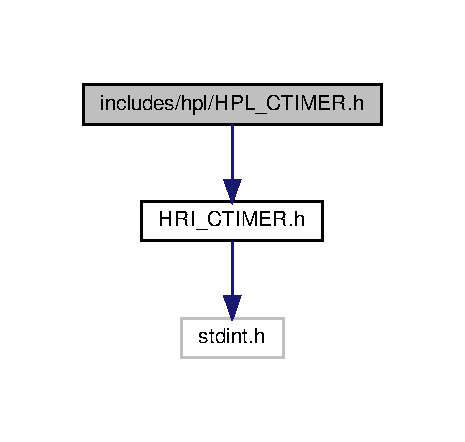
\includegraphics[width=223pt]{db/da7/HPL__CTIMER_8h__incl}
\end{center}
\end{figure}
Gráfico de los archivos que directa o indirectamente incluyen a este archivo\+:\nopagebreak
\begin{figure}[H]
\begin{center}
\leavevmode
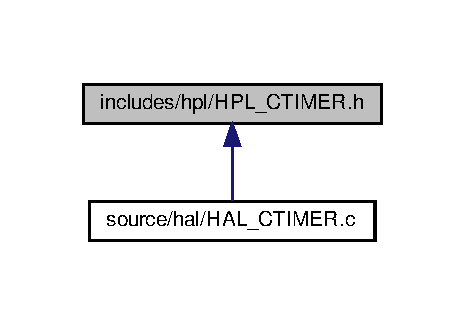
\includegraphics[width=223pt]{d0/dac/HPL__CTIMER_8h__dep__incl}
\end{center}
\end{figure}
\subsection*{Estructuras de datos}
\begin{DoxyCompactItemize}
\item 
struct \hyperlink{structCTIMER__MR__config__t}{C\+T\+I\+M\+E\+R\+\_\+\+M\+R\+\_\+config\+\_\+t}
\item 
struct \hyperlink{structCTIMER__CC__config__t}{C\+T\+I\+M\+E\+R\+\_\+\+C\+C\+\_\+config\+\_\+t}
\item 
struct \hyperlink{HPL__CTIMER_8h_db/d46/structCTIMER__CTCR__config__t}{C\+T\+I\+M\+E\+R\+\_\+\+C\+T\+C\+R\+\_\+config\+\_\+t}
\item 
struct \hyperlink{HPL__CTIMER_8h_d7/d01/structCTIMER__EMR__config__t}{C\+T\+I\+M\+E\+R\+\_\+\+E\+M\+R\+\_\+config\+\_\+t}
\end{DoxyCompactItemize}
\subsection*{Enumeraciones}
\begin{DoxyCompactItemize}
\item 
\mbox{\Hypertarget{HPL__CTIMER_8h_af928ad22d833d18f756a2eeadf9e2b19}\label{HPL__CTIMER_8h_af928ad22d833d18f756a2eeadf9e2b19}} 
enum {\bfseries C\+T\+I\+M\+E\+R\+\_\+\+E\+M\+C\+\_\+config\+\_\+en} \{ {\bfseries C\+T\+I\+M\+E\+R\+\_\+\+E\+M\+C\+\_\+\+C\+O\+N\+F\+I\+G\+\_\+\+D\+O\+\_\+\+N\+O\+T\+H\+I\+NG} = 0, 
{\bfseries C\+T\+I\+M\+E\+R\+\_\+\+E\+M\+C\+\_\+\+C\+O\+N\+F\+I\+G\+\_\+\+C\+L\+E\+AR}, 
{\bfseries C\+T\+I\+M\+E\+R\+\_\+\+E\+M\+C\+\_\+\+C\+O\+N\+F\+I\+G\+\_\+\+S\+ET}, 
{\bfseries C\+T\+I\+M\+E\+R\+\_\+\+E\+M\+C\+\_\+\+C\+O\+N\+F\+I\+G\+\_\+\+T\+O\+G\+G\+LE}
 \}
\item 
\mbox{\Hypertarget{HPL__CTIMER_8h_a3f1fe1a67aba7d85c4c384f0ac2f9146}\label{HPL__CTIMER_8h_a3f1fe1a67aba7d85c4c384f0ac2f9146}} 
enum {\bfseries C\+T\+I\+M\+E\+R\+\_\+\+C\+T\+M\+O\+D\+E\+\_\+config\+\_\+en} \{ {\bfseries C\+T\+I\+M\+E\+R\+\_\+\+C\+T\+M\+O\+D\+E\+\_\+\+C\+O\+N\+F\+I\+G\+\_\+\+T\+I\+M\+E\+R\+\_\+\+M\+O\+DE} = 0, 
{\bfseries C\+T\+I\+M\+E\+R\+\_\+\+C\+T\+M\+O\+D\+E\+\_\+\+C\+O\+N\+F\+I\+G\+\_\+\+R\+I\+S\+I\+N\+G\+\_\+\+E\+D\+GE}, 
{\bfseries C\+T\+I\+M\+E\+R\+\_\+\+C\+T\+M\+O\+D\+E\+\_\+\+C\+O\+N\+F\+I\+G\+\_\+\+F\+A\+L\+L\+I\+N\+G\+\_\+\+E\+D\+GE}, 
{\bfseries C\+T\+I\+M\+E\+R\+\_\+\+C\+T\+M\+O\+D\+E\+\_\+\+C\+O\+N\+F\+I\+G\+\_\+\+D\+O\+U\+B\+L\+E\+\_\+\+E\+D\+GE}
 \}
\item 
\mbox{\Hypertarget{HPL__CTIMER_8h_a5ae62580297d949c9fd128a527b02aa5}\label{HPL__CTIMER_8h_a5ae62580297d949c9fd128a527b02aa5}} 
enum {\bfseries C\+T\+I\+M\+E\+R\+\_\+\+C\+I\+N\+S\+E\+L\+\_\+config\+\_\+en} \{ {\bfseries C\+T\+I\+M\+E\+R\+\_\+\+C\+I\+N\+S\+E\+L\+\_\+\+C\+O\+N\+F\+I\+G\+\_\+\+C\+A\+P0} = 0, 
{\bfseries C\+T\+I\+M\+E\+R\+\_\+\+C\+I\+N\+S\+E\+L\+\_\+\+C\+O\+N\+F\+I\+G\+\_\+\+C\+A\+P1}, 
{\bfseries C\+T\+I\+M\+E\+R\+\_\+\+C\+I\+N\+S\+E\+L\+\_\+\+C\+O\+N\+F\+I\+G\+\_\+\+C\+A\+P2}, 
{\bfseries C\+T\+I\+M\+E\+R\+\_\+\+C\+I\+N\+S\+E\+L\+\_\+\+C\+O\+N\+F\+I\+G\+\_\+\+C\+A\+P3}
 \}
\item 
\mbox{\Hypertarget{HPL__CTIMER_8h_a6ec341be1a3ee9c83eb87a75a32dec63}\label{HPL__CTIMER_8h_a6ec341be1a3ee9c83eb87a75a32dec63}} 
enum {\bfseries C\+T\+I\+M\+E\+R\+\_\+\+S\+E\+L\+C\+C\+\_\+config\+\_\+en} \{ \newline
{\bfseries C\+T\+I\+M\+E\+R\+\_\+\+S\+E\+L\+C\+C\+\_\+\+C\+O\+N\+F\+I\+G\+\_\+\+C\+H0\+\_\+\+R\+I\+S\+I\+NG} = 0, 
{\bfseries C\+T\+I\+M\+E\+R\+\_\+\+S\+E\+L\+C\+C\+\_\+\+C\+O\+N\+F\+I\+G\+\_\+\+C\+H0\+\_\+\+F\+A\+L\+L\+I\+NG}, 
{\bfseries C\+T\+I\+M\+E\+R\+\_\+\+S\+E\+L\+C\+C\+\_\+\+C\+O\+N\+F\+I\+G\+\_\+\+C\+H1\+\_\+\+R\+I\+S\+I\+NG}, 
{\bfseries C\+T\+I\+M\+E\+R\+\_\+\+S\+E\+L\+C\+C\+\_\+\+C\+O\+N\+F\+I\+G\+\_\+\+C\+H1\+\_\+\+F\+A\+L\+L\+I\+NG}, 
\newline
{\bfseries C\+T\+I\+M\+E\+R\+\_\+\+S\+E\+L\+C\+C\+\_\+\+C\+O\+N\+F\+I\+G\+\_\+\+C\+H2\+\_\+\+R\+I\+S\+I\+NG}, 
{\bfseries C\+T\+I\+M\+E\+R\+\_\+\+S\+E\+L\+C\+C\+\_\+\+C\+O\+N\+F\+I\+G\+\_\+\+C\+H2\+\_\+\+F\+A\+L\+L\+I\+NG}, 
{\bfseries C\+T\+I\+M\+E\+R\+\_\+\+S\+E\+L\+C\+C\+\_\+\+C\+O\+N\+F\+I\+G\+\_\+\+C\+H3\+\_\+\+R\+I\+S\+I\+NG}, 
{\bfseries C\+T\+I\+M\+E\+R\+\_\+\+S\+E\+L\+C\+C\+\_\+\+C\+O\+N\+F\+I\+G\+\_\+\+C\+H3\+\_\+\+F\+A\+L\+L\+I\+NG}
 \}
\item 
\mbox{\Hypertarget{HPL__CTIMER_8h_a6684a2bed0c670847086b40e414d10d4}\label{HPL__CTIMER_8h_a6684a2bed0c670847086b40e414d10d4}} 
enum {\bfseries C\+T\+I\+M\+E\+R\+\_\+match\+\_\+sel\+\_\+en} \{ {\bfseries C\+T\+I\+M\+E\+R\+\_\+\+M\+A\+T\+C\+H\+\_\+\+S\+E\+L\+\_\+0} = 0, 
{\bfseries C\+T\+I\+M\+E\+R\+\_\+\+M\+A\+T\+C\+H\+\_\+\+S\+E\+L\+\_\+1}, 
{\bfseries C\+T\+I\+M\+E\+R\+\_\+\+M\+A\+T\+C\+H\+\_\+\+S\+E\+L\+\_\+2}, 
{\bfseries C\+T\+I\+M\+E\+R\+\_\+\+M\+A\+T\+C\+H\+\_\+\+S\+E\+L\+\_\+3}
 \}
\item 
\mbox{\Hypertarget{HPL__CTIMER_8h_a0e00df05efb00db54b812f76a233a6cd}\label{HPL__CTIMER_8h_a0e00df05efb00db54b812f76a233a6cd}} 
enum {\bfseries C\+T\+I\+M\+E\+R\+\_\+capture\+\_\+sel\+\_\+en} \{ {\bfseries C\+T\+I\+M\+E\+R\+\_\+\+C\+A\+P\+T\+U\+R\+E\+\_\+\+S\+E\+L\+\_\+0} = 0, 
{\bfseries C\+T\+I\+M\+E\+R\+\_\+\+C\+A\+P\+T\+U\+R\+E\+\_\+\+S\+E\+L\+\_\+1}, 
{\bfseries C\+T\+I\+M\+E\+R\+\_\+\+C\+A\+P\+T\+U\+R\+E\+\_\+\+S\+E\+L\+\_\+2}, 
{\bfseries C\+T\+I\+M\+E\+R\+\_\+\+C\+A\+P\+T\+U\+R\+E\+\_\+\+S\+E\+L\+\_\+3}
 \}
\item 
\mbox{\Hypertarget{HPL__CTIMER_8h_a71294965d41d77a3fa7a7d886bef65d8}\label{HPL__CTIMER_8h_a71294965d41d77a3fa7a7d886bef65d8}} 
enum {\bfseries C\+T\+I\+M\+E\+R\+\_\+external\+\_\+match\+\_\+action\+\_\+en} \{ {\bfseries C\+T\+I\+M\+E\+R\+\_\+\+E\+X\+T\+E\+R\+N\+A\+L\+\_\+\+M\+A\+T\+C\+H\+\_\+\+D\+O\+\_\+\+N\+O\+T\+H\+I\+NG} = 0, 
{\bfseries C\+T\+I\+M\+E\+R\+\_\+\+E\+X\+T\+E\+R\+N\+A\+L\+\_\+\+M\+A\+T\+C\+H\+\_\+\+C\+L\+E\+AR}, 
{\bfseries C\+T\+I\+M\+E\+R\+\_\+\+E\+X\+T\+E\+R\+N\+A\+L\+\_\+\+M\+A\+T\+C\+H\+\_\+\+S\+ET}, 
{\bfseries C\+T\+I\+M\+E\+R\+\_\+\+E\+X\+T\+E\+R\+N\+A\+L\+\_\+\+M\+A\+T\+C\+H\+\_\+\+T\+O\+G\+G\+LE}
 \}
\item 
\mbox{\Hypertarget{HPL__CTIMER_8h_a77d4c14b5af2cc9def38720f1d4d1812}\label{HPL__CTIMER_8h_a77d4c14b5af2cc9def38720f1d4d1812}} 
enum {\bfseries C\+T\+I\+M\+E\+R\+\_\+mode\+\_\+en} \{ {\bfseries C\+T\+I\+M\+E\+R\+\_\+\+M\+O\+D\+E\+\_\+\+T\+I\+M\+ER} = 0, 
{\bfseries C\+T\+I\+M\+E\+R\+\_\+\+M\+O\+D\+E\+\_\+\+C\+O\+U\+N\+T\+E\+R\+\_\+\+R\+I\+S\+I\+N\+G\+\_\+\+E\+D\+GE}, 
{\bfseries C\+T\+I\+M\+E\+R\+\_\+\+M\+O\+D\+E\+\_\+\+C\+O\+U\+N\+T\+E\+R\+\_\+\+F\+A\+L\+L\+I\+N\+G\+\_\+\+E\+D\+GE}, 
{\bfseries C\+T\+I\+M\+E\+R\+\_\+\+M\+O\+D\+E\+\_\+\+C\+O\+U\+N\+T\+E\+R\+\_\+\+D\+U\+A\+L\+\_\+\+E\+D\+GE}
 \}
\item 
\mbox{\Hypertarget{HPL__CTIMER_8h_a8f54fcb7d048a1820a5ca749e01d0c6d}\label{HPL__CTIMER_8h_a8f54fcb7d048a1820a5ca749e01d0c6d}} 
enum {\bfseries C\+T\+I\+M\+E\+R\+\_\+count\+\_\+in\+\_\+en} \{ {\bfseries C\+T\+I\+M\+E\+R\+\_\+\+C\+O\+U\+N\+T\+\_\+\+I\+N\+\_\+\+C\+A\+P0} = 0, 
{\bfseries C\+T\+I\+M\+E\+R\+\_\+\+C\+O\+U\+N\+T\+\_\+\+I\+N\+\_\+\+C\+A\+P1}, 
{\bfseries C\+T\+I\+M\+E\+R\+\_\+\+C\+O\+U\+N\+T\+\_\+\+I\+N\+\_\+\+C\+A\+P2}
 \}
\item 
\mbox{\Hypertarget{HPL__CTIMER_8h_a4fe6ab5089c4c8b2ae92f9959091d4ec}\label{HPL__CTIMER_8h_a4fe6ab5089c4c8b2ae92f9959091d4ec}} 
enum {\bfseries C\+T\+I\+M\+E\+R\+\_\+capture\+\_\+reset\+\_\+edge\+\_\+en} \{ \newline
{\bfseries C\+T\+I\+M\+E\+R\+\_\+\+C\+A\+P\+T\+U\+R\+E\+\_\+\+R\+E\+S\+E\+T\+\_\+\+C\+H0\+\_\+\+R\+I\+S\+I\+N\+G\+\_\+\+E\+D\+GE} = 0, 
{\bfseries C\+T\+I\+M\+E\+R\+\_\+\+C\+A\+P\+T\+U\+R\+E\+\_\+\+R\+E\+S\+E\+T\+\_\+\+C\+H0\+\_\+\+F\+A\+L\+L\+I\+N\+G\+\_\+\+E\+D\+GE}, 
{\bfseries C\+T\+I\+M\+E\+R\+\_\+\+C\+A\+P\+T\+U\+R\+E\+\_\+\+R\+E\+S\+E\+T\+\_\+\+C\+H1\+\_\+\+R\+I\+S\+I\+N\+G\+\_\+\+E\+D\+GE}, 
{\bfseries C\+T\+I\+M\+E\+R\+\_\+\+C\+A\+P\+T\+U\+R\+E\+\_\+\+R\+E\+S\+E\+T\+\_\+\+C\+H1\+\_\+\+F\+A\+L\+L\+I\+N\+G\+\_\+\+E\+D\+GE}, 
\newline
{\bfseries C\+T\+I\+M\+E\+R\+\_\+\+C\+A\+P\+T\+U\+R\+E\+\_\+\+R\+E\+S\+E\+T\+\_\+\+C\+H2\+\_\+\+R\+I\+S\+I\+N\+G\+\_\+\+E\+D\+GE}, 
{\bfseries C\+T\+I\+M\+E\+R\+\_\+\+C\+A\+P\+T\+U\+R\+E\+\_\+\+R\+E\+S\+E\+T\+\_\+\+C\+H2\+\_\+\+F\+A\+L\+L\+I\+N\+G\+\_\+\+E\+D\+GE}, 
{\bfseries C\+T\+I\+M\+E\+R\+\_\+\+C\+A\+P\+T\+U\+R\+E\+\_\+\+R\+E\+S\+E\+T\+\_\+\+C\+H3\+\_\+\+R\+I\+S\+I\+N\+G\+\_\+\+E\+D\+GE}, 
{\bfseries C\+T\+I\+M\+E\+R\+\_\+\+C\+A\+P\+T\+U\+R\+E\+\_\+\+R\+E\+S\+E\+T\+\_\+\+C\+H3\+\_\+\+F\+A\+L\+L\+I\+N\+G\+\_\+\+E\+D\+GE}
 \}
\item 
\mbox{\Hypertarget{HPL__CTIMER_8h_a4e02f1bf48b11dc8eba13f67d299b547}\label{HPL__CTIMER_8h_a4e02f1bf48b11dc8eba13f67d299b547}} 
enum {\bfseries C\+T\+I\+M\+E\+R\+\_\+pwm\+\_\+channel\+\_\+en} \{ {\bfseries C\+T\+I\+M\+E\+R\+\_\+\+P\+W\+M\+\_\+\+C\+H\+A\+N\+N\+E\+L\+\_\+0} = 0, 
{\bfseries C\+T\+I\+M\+E\+R\+\_\+\+P\+W\+M\+\_\+\+C\+H\+A\+N\+N\+E\+L\+\_\+1}, 
{\bfseries C\+T\+I\+M\+E\+R\+\_\+\+P\+W\+M\+\_\+\+C\+H\+A\+N\+N\+E\+L\+\_\+2}
 \}
\end{DoxyCompactItemize}
\subsection*{Funciones}
\begin{DoxyCompactItemize}
\item 
static uint8\+\_\+t \hyperlink{HPL__CTIMER_8h_a27f58db77aa91c27bb58b4dc22c91e2b}{C\+T\+I\+M\+E\+R\+\_\+get\+\_\+match\+\_\+irq\+\_\+flag} (C\+T\+I\+M\+E\+R\+\_\+match\+\_\+sel\+\_\+en match)
\begin{DoxyCompactList}\small\item\em Obtener estado de flag de interrupcion de algun match. \end{DoxyCompactList}\item 
static uint8\+\_\+t \hyperlink{HPL__CTIMER_8h_a2f08c330c1bab94262042334e4522337}{C\+T\+I\+M\+E\+R\+\_\+get\+\_\+capture\+\_\+irq\+\_\+flag} (C\+T\+I\+M\+E\+R\+\_\+capture\+\_\+sel\+\_\+en capture)
\begin{DoxyCompactList}\small\item\em Obtener estado de flag de interrupcion de algun capture. \end{DoxyCompactList}\item 
static void \hyperlink{HPL__CTIMER_8h_a02278e366d5b2bba8e5f0283f27fceb1}{C\+T\+I\+M\+E\+R\+\_\+clear\+\_\+match\+\_\+irq\+\_\+flag} (C\+T\+I\+M\+E\+R\+\_\+match\+\_\+sel\+\_\+en match)
\begin{DoxyCompactList}\small\item\em Limpiar flag de interrupcion de match. \end{DoxyCompactList}\item 
static void \hyperlink{HPL__CTIMER_8h_ab5afd3ccd798e81cfa7fd0ba53c93d2f}{C\+T\+I\+M\+E\+R\+\_\+clear\+\_\+capture\+\_\+irq\+\_\+flag} (C\+T\+I\+M\+E\+R\+\_\+capture\+\_\+sel\+\_\+en capture)
\begin{DoxyCompactList}\small\item\em Limpiar flag de interrupcion de capture. \end{DoxyCompactList}\item 
\mbox{\Hypertarget{HPL__CTIMER_8h_a06102d2946e10f19b8802ad5ef7d2cf2}\label{HPL__CTIMER_8h_a06102d2946e10f19b8802ad5ef7d2cf2}} 
static void \hyperlink{HPL__CTIMER_8h_a06102d2946e10f19b8802ad5ef7d2cf2}{C\+T\+I\+M\+E\+R\+\_\+enable\+\_\+counter} (void)
\begin{DoxyCompactList}\small\item\em Habilitar el contador. \end{DoxyCompactList}\item 
\mbox{\Hypertarget{HPL__CTIMER_8h_a529c8e39e28441bd0e36197782b71de5}\label{HPL__CTIMER_8h_a529c8e39e28441bd0e36197782b71de5}} 
static void \hyperlink{HPL__CTIMER_8h_a529c8e39e28441bd0e36197782b71de5}{C\+T\+I\+M\+E\+R\+\_\+disable\+\_\+counter} (void)
\begin{DoxyCompactList}\small\item\em Inhabilitar el contador. \end{DoxyCompactList}\item 
\mbox{\Hypertarget{HPL__CTIMER_8h_aeb8cc3dc974555acf640f29de584cc3d}\label{HPL__CTIMER_8h_aeb8cc3dc974555acf640f29de584cc3d}} 
static void \hyperlink{HPL__CTIMER_8h_aeb8cc3dc974555acf640f29de584cc3d}{C\+T\+I\+M\+E\+R\+\_\+assert\+\_\+counter\+\_\+reset} (void)
\begin{DoxyCompactList}\small\item\em Accionar el reset del contador. \end{DoxyCompactList}\item 
\mbox{\Hypertarget{HPL__CTIMER_8h_a32d33ac3c7011c4f9c931b227053fb1c}\label{HPL__CTIMER_8h_a32d33ac3c7011c4f9c931b227053fb1c}} 
static void \hyperlink{HPL__CTIMER_8h_a32d33ac3c7011c4f9c931b227053fb1c}{C\+T\+I\+M\+E\+R\+\_\+clear\+\_\+counter\+\_\+reset} (void)
\begin{DoxyCompactList}\small\item\em Limpiar el reset del contador. \end{DoxyCompactList}\item 
static void \hyperlink{HPL__CTIMER_8h_a4a09c347d419c5e761d2d8b2cff4b646}{C\+T\+I\+M\+E\+R\+\_\+write\+\_\+counter} (uint32\+\_\+t value)
\begin{DoxyCompactList}\small\item\em Escribir conteo. \end{DoxyCompactList}\item 
static uint32\+\_\+t \hyperlink{HPL__CTIMER_8h_a91b7495b9001807664b3613d227dee65}{C\+T\+I\+M\+E\+R\+\_\+read\+\_\+counter} (void)
\begin{DoxyCompactList}\small\item\em Leer valor de conteo actual. \end{DoxyCompactList}\item 
static void \hyperlink{HPL__CTIMER_8h_a42ec527736e7adf1cc560d9c4918a909}{C\+T\+I\+M\+E\+R\+\_\+write\+\_\+prescaler} (uint32\+\_\+t value)
\begin{DoxyCompactList}\small\item\em Escribir valor de prescaler. \end{DoxyCompactList}\item 
static uint32\+\_\+t \hyperlink{HPL__CTIMER_8h_a5c85c03ad0e02e34aa0a878f5a3f8a1a}{C\+T\+I\+M\+E\+R\+\_\+read\+\_\+prescaler} (void)
\begin{DoxyCompactList}\small\item\em Leer el valor del prescaler. \end{DoxyCompactList}\item 
static void \hyperlink{HPL__CTIMER_8h_ac94ae7e453c538f62dbb50b758ac4cec}{C\+T\+I\+M\+E\+R\+\_\+enable\+\_\+interrupt\+\_\+on\+\_\+match} (C\+T\+I\+M\+E\+R\+\_\+match\+\_\+sel\+\_\+en match)
\begin{DoxyCompactList}\small\item\em Habilitar interrupcion en match. \end{DoxyCompactList}\item 
static void \hyperlink{HPL__CTIMER_8h_af570a1acf253b98b8d3ea2677896b5f6}{C\+T\+I\+M\+E\+R\+\_\+disable\+\_\+interrupt\+\_\+on\+\_\+match} (C\+T\+I\+M\+E\+R\+\_\+match\+\_\+sel\+\_\+en match)
\begin{DoxyCompactList}\small\item\em Inhabilitar interrupcion en match. \end{DoxyCompactList}\item 
static void \hyperlink{HPL__CTIMER_8h_a5cd9b664313ff34738259160c707ce43}{C\+T\+I\+M\+E\+R\+\_\+enable\+\_\+reset\+\_\+on\+\_\+match} (C\+T\+I\+M\+E\+R\+\_\+match\+\_\+sel\+\_\+en match)
\begin{DoxyCompactList}\small\item\em Habilitar reset en match. \end{DoxyCompactList}\item 
static void \hyperlink{HPL__CTIMER_8h_afc1cf25a3c8b142ec2b68c4fe8fc456c}{C\+T\+I\+M\+E\+R\+\_\+disable\+\_\+reset\+\_\+on\+\_\+match} (C\+T\+I\+M\+E\+R\+\_\+match\+\_\+sel\+\_\+en match)
\begin{DoxyCompactList}\small\item\em Inhabilitar reset en match. \end{DoxyCompactList}\item 
static void \hyperlink{HPL__CTIMER_8h_a62eb47a45ab7070f3bb40fb66182f153}{C\+T\+I\+M\+E\+R\+\_\+enable\+\_\+stop\+\_\+on\+\_\+match} (C\+T\+I\+M\+E\+R\+\_\+match\+\_\+sel\+\_\+en match)
\begin{DoxyCompactList}\small\item\em Habilitar stop en match. \end{DoxyCompactList}\item 
static void \hyperlink{HPL__CTIMER_8h_a2467c66ac8cf923c094b0bc3f279a6b9}{C\+T\+I\+M\+E\+R\+\_\+disable\+\_\+stop\+\_\+on\+\_\+match} (C\+T\+I\+M\+E\+R\+\_\+match\+\_\+sel\+\_\+en match)
\begin{DoxyCompactList}\small\item\em Inhabilitar stop en match. \end{DoxyCompactList}\item 
static void \hyperlink{HPL__CTIMER_8h_a5d091e95e0ab42266c9da7a0afef41a9}{C\+T\+I\+M\+E\+R\+\_\+enable\+\_\+reload\+\_\+on\+\_\+match} (C\+T\+I\+M\+E\+R\+\_\+match\+\_\+sel\+\_\+en match)
\begin{DoxyCompactList}\small\item\em Habilitar reload en match. \end{DoxyCompactList}\item 
static void \hyperlink{HPL__CTIMER_8h_af19c694590afb2191cf2fbefc43259ac}{C\+T\+I\+M\+E\+R\+\_\+disable\+\_\+reload\+\_\+on\+\_\+match} (C\+T\+I\+M\+E\+R\+\_\+match\+\_\+sel\+\_\+en match)
\begin{DoxyCompactList}\small\item\em Inhabilitar reload en match. \end{DoxyCompactList}\item 
static void \hyperlink{HPL__CTIMER_8h_af235f6203f9261b7247aa8f2fb6259e5}{C\+T\+I\+M\+E\+R\+\_\+write\+\_\+match\+\_\+value} (C\+T\+I\+M\+E\+R\+\_\+match\+\_\+sel\+\_\+en match, uint32\+\_\+t value)
\begin{DoxyCompactList}\small\item\em Escribir un registro de match. \end{DoxyCompactList}\item 
static uint32\+\_\+t \hyperlink{HPL__CTIMER_8h_a0c67ada8fa3f35a67fb3581619d9d725}{C\+T\+I\+M\+E\+R\+\_\+read\+\_\+match\+\_\+value} (C\+T\+I\+M\+E\+R\+\_\+match\+\_\+sel\+\_\+en match)
\begin{DoxyCompactList}\small\item\em Leer un registro de match. \end{DoxyCompactList}\item 
static void \hyperlink{HPL__CTIMER_8h_afc2b3db7bd1f92634e37282aa97fbf11}{C\+T\+I\+M\+E\+R\+\_\+enable\+\_\+rising\+\_\+edge\+\_\+capture} (C\+T\+I\+M\+E\+R\+\_\+capture\+\_\+sel\+\_\+en capture)
\begin{DoxyCompactList}\small\item\em Habilitar captura en flanco ascendente. \end{DoxyCompactList}\item 
static void \hyperlink{HPL__CTIMER_8h_a605f604bdf706687cd9e95d03ac73970}{C\+T\+I\+M\+E\+R\+\_\+disable\+\_\+rising\+\_\+edge\+\_\+capture} (C\+T\+I\+M\+E\+R\+\_\+capture\+\_\+sel\+\_\+en capture)
\begin{DoxyCompactList}\small\item\em Inhabilitar captura en flanco ascendente. \end{DoxyCompactList}\item 
static void \hyperlink{HPL__CTIMER_8h_acd4a2d9d965de648290fb19e08f14d40}{C\+T\+I\+M\+E\+R\+\_\+enable\+\_\+falling\+\_\+edge\+\_\+capture} (C\+T\+I\+M\+E\+R\+\_\+capture\+\_\+sel\+\_\+en capture)
\begin{DoxyCompactList}\small\item\em Habilitar captura en flanco descendente. \end{DoxyCompactList}\item 
static void \hyperlink{HPL__CTIMER_8h_a6fb57e3ec340ae4d678fab5585c14458}{C\+T\+I\+M\+E\+R\+\_\+disable\+\_\+falling\+\_\+edge\+\_\+capture} (C\+T\+I\+M\+E\+R\+\_\+capture\+\_\+sel\+\_\+en capture)
\begin{DoxyCompactList}\small\item\em Inhabilitar captura en flanco descendente. \end{DoxyCompactList}\item 
static void \hyperlink{HPL__CTIMER_8h_a9af81d869d38a2ac20a39d47cf34b2cf}{C\+T\+I\+M\+E\+R\+\_\+enable\+\_\+interrupt\+\_\+on\+\_\+capture} (C\+T\+I\+M\+E\+R\+\_\+capture\+\_\+sel\+\_\+en capture)
\begin{DoxyCompactList}\small\item\em Habilitar interrupcion en captura. \end{DoxyCompactList}\item 
static void \hyperlink{HPL__CTIMER_8h_a34c093f3fd326baef174bbe5da35a938}{C\+T\+I\+M\+E\+R\+\_\+disable\+\_\+interrupt\+\_\+on\+\_\+capture} (C\+T\+I\+M\+E\+R\+\_\+capture\+\_\+sel\+\_\+en capture)
\begin{DoxyCompactList}\small\item\em Inhabilitar interrupcion en captura. \end{DoxyCompactList}\item 
static uint32\+\_\+t \hyperlink{HPL__CTIMER_8h_a3e3b8370e211113b7b0043f609a61697}{C\+T\+I\+M\+E\+R\+\_\+read\+\_\+capture\+\_\+value} (C\+T\+I\+M\+E\+R\+\_\+capture\+\_\+sel\+\_\+en capture)
\begin{DoxyCompactList}\small\item\em Leer registro de captura. \end{DoxyCompactList}\item 
static uint8\+\_\+t \hyperlink{HPL__CTIMER_8h_a1b55bf06c9f93d0918c8b10aea9edeed}{C\+T\+I\+M\+E\+R\+\_\+read\+\_\+match\+\_\+status} (C\+T\+I\+M\+E\+R\+\_\+match\+\_\+sel\+\_\+en match)
\begin{DoxyCompactList}\small\item\em Leer estado de match externo. \end{DoxyCompactList}\item 
static void \hyperlink{HPL__CTIMER_8h_aadf0218b584d38881950dff1e92db07d}{C\+T\+I\+M\+E\+R\+\_\+config\+\_\+external\+\_\+match} (C\+T\+I\+M\+E\+R\+\_\+match\+\_\+sel\+\_\+en match, C\+T\+I\+M\+E\+R\+\_\+external\+\_\+match\+\_\+action\+\_\+en action)
\begin{DoxyCompactList}\small\item\em Configurar accion en match externo. \end{DoxyCompactList}\item 
static void \hyperlink{HPL__CTIMER_8h_a6798b925cb94fc45b0f249f3c4a9caf4}{C\+T\+I\+M\+E\+R\+\_\+config\+\_\+counter\+\_\+timer\+\_\+mode} (C\+T\+I\+M\+E\+R\+\_\+mode\+\_\+en mode)
\begin{DoxyCompactList}\small\item\em Configurar modo de funcionamiento. \end{DoxyCompactList}\item 
static void \hyperlink{HPL__CTIMER_8h_a7a4d992f6953fb02924c7737c861bd79}{C\+T\+I\+M\+E\+R\+\_\+config\+\_\+counter\+\_\+input} (C\+T\+I\+M\+E\+R\+\_\+count\+\_\+in\+\_\+en count\+\_\+in)
\begin{DoxyCompactList}\small\item\em Configurar entrada de conteo (modo counter rising/falling/dual edge) \end{DoxyCompactList}\item 
\mbox{\Hypertarget{HPL__CTIMER_8h_a68baceeab28547d0fb2b05857fc970c0}\label{HPL__CTIMER_8h_a68baceeab28547d0fb2b05857fc970c0}} 
static void \hyperlink{HPL__CTIMER_8h_a68baceeab28547d0fb2b05857fc970c0}{C\+T\+I\+M\+E\+R\+\_\+enable\+\_\+count\+\_\+reset\+\_\+on\+\_\+capture} (void)
\begin{DoxyCompactList}\small\item\em Habilitar reset de conteo y prescaler en captura. \end{DoxyCompactList}\item 
\mbox{\Hypertarget{HPL__CTIMER_8h_a45fa3e21b83935acc1238b622b088f3a}\label{HPL__CTIMER_8h_a45fa3e21b83935acc1238b622b088f3a}} 
static void \hyperlink{HPL__CTIMER_8h_a45fa3e21b83935acc1238b622b088f3a}{C\+T\+I\+M\+E\+R\+\_\+disable\+\_\+count\+\_\+reset\+\_\+on\+\_\+capture} (void)
\begin{DoxyCompactList}\small\item\em Inhabilitar reset de conteo y prescaler en captura. \end{DoxyCompactList}\item 
static void \hyperlink{HPL__CTIMER_8h_a259b66e8bfdc6189db35771e14260fc9}{C\+T\+I\+M\+E\+R\+\_\+config\+\_\+capture\+\_\+reset} (C\+T\+I\+M\+E\+R\+\_\+capture\+\_\+reset\+\_\+edge\+\_\+en capture\+\_\+sel)
\begin{DoxyCompactList}\small\item\em Configurar captura que genera reset de conteo y prescaler (si esta habilitado) \end{DoxyCompactList}\item 
static void \hyperlink{HPL__CTIMER_8h_a4b1bc88a3c5f6892f3aab229298b077d}{C\+T\+I\+M\+E\+R\+\_\+enable\+\_\+pwm} (C\+T\+I\+M\+E\+R\+\_\+pwm\+\_\+channel\+\_\+en pwm)
\begin{DoxyCompactList}\small\item\em Habilitar canal de P\+WM. \end{DoxyCompactList}\item 
static void \hyperlink{HPL__CTIMER_8h_a352d401a756799aee87c1163655764af}{C\+T\+I\+M\+E\+R\+\_\+disable\+\_\+pwm} (C\+T\+I\+M\+E\+R\+\_\+pwm\+\_\+channel\+\_\+en pwm)
\begin{DoxyCompactList}\small\item\em Inhabilitar canal de P\+WM. \end{DoxyCompactList}\item 
static void \hyperlink{HPL__CTIMER_8h_ae4feb6e8e07b4362382c66cc8c2aa79b}{C\+T\+I\+M\+E\+R\+\_\+write\+\_\+shadow\+\_\+register} (C\+T\+I\+M\+E\+R\+\_\+match\+\_\+sel\+\_\+en match, uint32\+\_\+t value)
\begin{DoxyCompactList}\small\item\em Escribir registros fantasma de match. \end{DoxyCompactList}\end{DoxyCompactItemize}
\subsection*{Variables}
\begin{DoxyCompactItemize}
\item 
\mbox{\Hypertarget{HPL__CTIMER_8h_a8150dcb6b90800d1dfe8669e1f21f549}\label{HPL__CTIMER_8h_a8150dcb6b90800d1dfe8669e1f21f549}} 
volatile \hyperlink{HRI__CTIMER_8h_d1/de3/structCTIMER__per__t}{C\+T\+I\+M\+E\+R\+\_\+per\+\_\+t} $\ast$const \hyperlink{HPL__CTIMER_8h_a8150dcb6b90800d1dfe8669e1f21f549}{C\+T\+I\+M\+ER}
\begin{DoxyCompactList}\small\item\em Periferico C\+T\+I\+M\+ER. \end{DoxyCompactList}\end{DoxyCompactItemize}


\subsection{Descripción detallada}
Definiciones a nivel de abstraccion del periferico C\+T\+I\+M\+ER (L\+P\+C845) 

\begin{DoxyAuthor}{Autor}
Augusto Santini 
\end{DoxyAuthor}
\begin{DoxyDate}{Fecha}
3/2020 
\end{DoxyDate}
\begin{DoxyVersion}{Versión}
1.\+0 
\end{DoxyVersion}


\subsection{Documentación de las estructuras de datos}
\index{C\+T\+I\+M\+E\+R\+\_\+\+C\+T\+C\+R\+\_\+config\+\_\+t@{C\+T\+I\+M\+E\+R\+\_\+\+C\+T\+C\+R\+\_\+config\+\_\+t}}\label{structCTIMER__CTCR__config__t}
\Hypertarget{HPL__CTIMER_8h_structCTIMER__CTCR__config__t}
\subsubsection{struct C\+T\+I\+M\+E\+R\+\_\+\+C\+T\+C\+R\+\_\+config\+\_\+t}
\begin{DoxyFields}{Campos de datos}
\mbox{\Hypertarget{HPL__CTIMER_8h_a811f4b8928005a600b0e6d759ef618ea}\label{HPL__CTIMER_8h_a811f4b8928005a600b0e6d759ef618ea}} 
CTIMER\_CTMODE\_config\_en&
CTMODE&
\\
\hline

\mbox{\Hypertarget{HPL__CTIMER_8h_a97b7d399f4822bd1f54944b3802014d4}\label{HPL__CTIMER_8h_a97b7d399f4822bd1f54944b3802014d4}} 
CTIMER\_CINSEL\_config\_en&
CINSEL&
\\
\hline

\mbox{\Hypertarget{HPL__CTIMER_8h_aeddd5c43fb661be27ce9806df57ba1c4}\label{HPL__CTIMER_8h_aeddd5c43fb661be27ce9806df57ba1c4}} 
uint8\_t&
ENCC&
\\
\hline

\mbox{\Hypertarget{HPL__CTIMER_8h_a23d7dfc8be8a94623276db706356e066}\label{HPL__CTIMER_8h_a23d7dfc8be8a94623276db706356e066}} 
CTIMER\_SELCC\_config\_en&
SELCC&
\\
\hline

\end{DoxyFields}
\index{C\+T\+I\+M\+E\+R\+\_\+\+E\+M\+R\+\_\+config\+\_\+t@{C\+T\+I\+M\+E\+R\+\_\+\+E\+M\+R\+\_\+config\+\_\+t}}\label{structCTIMER__EMR__config__t}
\Hypertarget{HPL__CTIMER_8h_structCTIMER__EMR__config__t}
\subsubsection{struct C\+T\+I\+M\+E\+R\+\_\+\+E\+M\+R\+\_\+config\+\_\+t}
\begin{DoxyFields}{Campos de datos}
\mbox{\Hypertarget{HPL__CTIMER_8h_a045d8792b3c1b5e3590a04258a6f6e03}\label{HPL__CTIMER_8h_a045d8792b3c1b5e3590a04258a6f6e03}} 
CTIMER\_EMC\_config\_en&
EMC&
\\
\hline

\mbox{\Hypertarget{HPL__CTIMER_8h_a48ab702d15103d11869acaeb9d0d1526}\label{HPL__CTIMER_8h_a48ab702d15103d11869acaeb9d0d1526}} 
uint8\_t&
mat\_enable&
\\
\hline

\mbox{\Hypertarget{HPL__CTIMER_8h_a370bb6219d7674f84de88cae6d20d18d}\label{HPL__CTIMER_8h_a370bb6219d7674f84de88cae6d20d18d}} 
uint8\_t&
mat\_port&
\\
\hline

\mbox{\Hypertarget{HPL__CTIMER_8h_ac960df15af423ab34179e05a8d515297}\label{HPL__CTIMER_8h_ac960df15af423ab34179e05a8d515297}} 
uint8\_t&
mat\_pin&
\\
\hline

\end{DoxyFields}


\subsection{Documentación de las funciones}
\mbox{\Hypertarget{HPL__CTIMER_8h_a27f58db77aa91c27bb58b4dc22c91e2b}\label{HPL__CTIMER_8h_a27f58db77aa91c27bb58b4dc22c91e2b}} 
\index{H\+P\+L\+\_\+\+C\+T\+I\+M\+E\+R.\+h@{H\+P\+L\+\_\+\+C\+T\+I\+M\+E\+R.\+h}!C\+T\+I\+M\+E\+R\+\_\+get\+\_\+match\+\_\+irq\+\_\+flag@{C\+T\+I\+M\+E\+R\+\_\+get\+\_\+match\+\_\+irq\+\_\+flag}}
\index{C\+T\+I\+M\+E\+R\+\_\+get\+\_\+match\+\_\+irq\+\_\+flag@{C\+T\+I\+M\+E\+R\+\_\+get\+\_\+match\+\_\+irq\+\_\+flag}!H\+P\+L\+\_\+\+C\+T\+I\+M\+E\+R.\+h@{H\+P\+L\+\_\+\+C\+T\+I\+M\+E\+R.\+h}}
\subsubsection{\texorpdfstring{C\+T\+I\+M\+E\+R\+\_\+get\+\_\+match\+\_\+irq\+\_\+flag()}{CTIMER\_get\_match\_irq\_flag()}}
{\footnotesize\ttfamily static uint8\+\_\+t C\+T\+I\+M\+E\+R\+\_\+get\+\_\+match\+\_\+irq\+\_\+flag (\begin{DoxyParamCaption}\item[{C\+T\+I\+M\+E\+R\+\_\+match\+\_\+sel\+\_\+en}]{match }\end{DoxyParamCaption})\hspace{0.3cm}{\ttfamily [inline]}, {\ttfamily [static]}}



Obtener estado de flag de interrupcion de algun match. 


\begin{DoxyParams}[1]{Parámetros}
\mbox{\tt in}  & {\em match} & Numero de match a consultar \\
\hline
\end{DoxyParams}
\begin{DoxyReturn}{Devuelve}
Valor del flag actual 
\end{DoxyReturn}
\mbox{\Hypertarget{HPL__CTIMER_8h_a2f08c330c1bab94262042334e4522337}\label{HPL__CTIMER_8h_a2f08c330c1bab94262042334e4522337}} 
\index{H\+P\+L\+\_\+\+C\+T\+I\+M\+E\+R.\+h@{H\+P\+L\+\_\+\+C\+T\+I\+M\+E\+R.\+h}!C\+T\+I\+M\+E\+R\+\_\+get\+\_\+capture\+\_\+irq\+\_\+flag@{C\+T\+I\+M\+E\+R\+\_\+get\+\_\+capture\+\_\+irq\+\_\+flag}}
\index{C\+T\+I\+M\+E\+R\+\_\+get\+\_\+capture\+\_\+irq\+\_\+flag@{C\+T\+I\+M\+E\+R\+\_\+get\+\_\+capture\+\_\+irq\+\_\+flag}!H\+P\+L\+\_\+\+C\+T\+I\+M\+E\+R.\+h@{H\+P\+L\+\_\+\+C\+T\+I\+M\+E\+R.\+h}}
\subsubsection{\texorpdfstring{C\+T\+I\+M\+E\+R\+\_\+get\+\_\+capture\+\_\+irq\+\_\+flag()}{CTIMER\_get\_capture\_irq\_flag()}}
{\footnotesize\ttfamily static uint8\+\_\+t C\+T\+I\+M\+E\+R\+\_\+get\+\_\+capture\+\_\+irq\+\_\+flag (\begin{DoxyParamCaption}\item[{C\+T\+I\+M\+E\+R\+\_\+capture\+\_\+sel\+\_\+en}]{capture }\end{DoxyParamCaption})\hspace{0.3cm}{\ttfamily [inline]}, {\ttfamily [static]}}



Obtener estado de flag de interrupcion de algun capture. 


\begin{DoxyParams}[1]{Parámetros}
\mbox{\tt in}  & {\em match} & Numero de capture a consultar \\
\hline
\end{DoxyParams}
\begin{DoxyReturn}{Devuelve}
Valor del flag actual 
\end{DoxyReturn}
\mbox{\Hypertarget{HPL__CTIMER_8h_a02278e366d5b2bba8e5f0283f27fceb1}\label{HPL__CTIMER_8h_a02278e366d5b2bba8e5f0283f27fceb1}} 
\index{H\+P\+L\+\_\+\+C\+T\+I\+M\+E\+R.\+h@{H\+P\+L\+\_\+\+C\+T\+I\+M\+E\+R.\+h}!C\+T\+I\+M\+E\+R\+\_\+clear\+\_\+match\+\_\+irq\+\_\+flag@{C\+T\+I\+M\+E\+R\+\_\+clear\+\_\+match\+\_\+irq\+\_\+flag}}
\index{C\+T\+I\+M\+E\+R\+\_\+clear\+\_\+match\+\_\+irq\+\_\+flag@{C\+T\+I\+M\+E\+R\+\_\+clear\+\_\+match\+\_\+irq\+\_\+flag}!H\+P\+L\+\_\+\+C\+T\+I\+M\+E\+R.\+h@{H\+P\+L\+\_\+\+C\+T\+I\+M\+E\+R.\+h}}
\subsubsection{\texorpdfstring{C\+T\+I\+M\+E\+R\+\_\+clear\+\_\+match\+\_\+irq\+\_\+flag()}{CTIMER\_clear\_match\_irq\_flag()}}
{\footnotesize\ttfamily static void C\+T\+I\+M\+E\+R\+\_\+clear\+\_\+match\+\_\+irq\+\_\+flag (\begin{DoxyParamCaption}\item[{C\+T\+I\+M\+E\+R\+\_\+match\+\_\+sel\+\_\+en}]{match }\end{DoxyParamCaption})\hspace{0.3cm}{\ttfamily [inline]}, {\ttfamily [static]}}



Limpiar flag de interrupcion de match. 


\begin{DoxyParams}[1]{Parámetros}
\mbox{\tt in}  & {\em match} & Numero de match a limpiar \\
\hline
\end{DoxyParams}
\mbox{\Hypertarget{HPL__CTIMER_8h_ab5afd3ccd798e81cfa7fd0ba53c93d2f}\label{HPL__CTIMER_8h_ab5afd3ccd798e81cfa7fd0ba53c93d2f}} 
\index{H\+P\+L\+\_\+\+C\+T\+I\+M\+E\+R.\+h@{H\+P\+L\+\_\+\+C\+T\+I\+M\+E\+R.\+h}!C\+T\+I\+M\+E\+R\+\_\+clear\+\_\+capture\+\_\+irq\+\_\+flag@{C\+T\+I\+M\+E\+R\+\_\+clear\+\_\+capture\+\_\+irq\+\_\+flag}}
\index{C\+T\+I\+M\+E\+R\+\_\+clear\+\_\+capture\+\_\+irq\+\_\+flag@{C\+T\+I\+M\+E\+R\+\_\+clear\+\_\+capture\+\_\+irq\+\_\+flag}!H\+P\+L\+\_\+\+C\+T\+I\+M\+E\+R.\+h@{H\+P\+L\+\_\+\+C\+T\+I\+M\+E\+R.\+h}}
\subsubsection{\texorpdfstring{C\+T\+I\+M\+E\+R\+\_\+clear\+\_\+capture\+\_\+irq\+\_\+flag()}{CTIMER\_clear\_capture\_irq\_flag()}}
{\footnotesize\ttfamily static void C\+T\+I\+M\+E\+R\+\_\+clear\+\_\+capture\+\_\+irq\+\_\+flag (\begin{DoxyParamCaption}\item[{C\+T\+I\+M\+E\+R\+\_\+capture\+\_\+sel\+\_\+en}]{capture }\end{DoxyParamCaption})\hspace{0.3cm}{\ttfamily [inline]}, {\ttfamily [static]}}



Limpiar flag de interrupcion de capture. 


\begin{DoxyParams}[1]{Parámetros}
\mbox{\tt in}  & {\em match} & Numero de capture a limpiar \\
\hline
\end{DoxyParams}
\mbox{\Hypertarget{HPL__CTIMER_8h_a4a09c347d419c5e761d2d8b2cff4b646}\label{HPL__CTIMER_8h_a4a09c347d419c5e761d2d8b2cff4b646}} 
\index{H\+P\+L\+\_\+\+C\+T\+I\+M\+E\+R.\+h@{H\+P\+L\+\_\+\+C\+T\+I\+M\+E\+R.\+h}!C\+T\+I\+M\+E\+R\+\_\+write\+\_\+counter@{C\+T\+I\+M\+E\+R\+\_\+write\+\_\+counter}}
\index{C\+T\+I\+M\+E\+R\+\_\+write\+\_\+counter@{C\+T\+I\+M\+E\+R\+\_\+write\+\_\+counter}!H\+P\+L\+\_\+\+C\+T\+I\+M\+E\+R.\+h@{H\+P\+L\+\_\+\+C\+T\+I\+M\+E\+R.\+h}}
\subsubsection{\texorpdfstring{C\+T\+I\+M\+E\+R\+\_\+write\+\_\+counter()}{CTIMER\_write\_counter()}}
{\footnotesize\ttfamily static void C\+T\+I\+M\+E\+R\+\_\+write\+\_\+counter (\begin{DoxyParamCaption}\item[{uint32\+\_\+t}]{value }\end{DoxyParamCaption})\hspace{0.3cm}{\ttfamily [inline]}, {\ttfamily [static]}}



Escribir conteo. 


\begin{DoxyParams}[1]{Parámetros}
\mbox{\tt in}  & {\em value} & Valor deseado \\
\hline
\end{DoxyParams}
\mbox{\Hypertarget{HPL__CTIMER_8h_a91b7495b9001807664b3613d227dee65}\label{HPL__CTIMER_8h_a91b7495b9001807664b3613d227dee65}} 
\index{H\+P\+L\+\_\+\+C\+T\+I\+M\+E\+R.\+h@{H\+P\+L\+\_\+\+C\+T\+I\+M\+E\+R.\+h}!C\+T\+I\+M\+E\+R\+\_\+read\+\_\+counter@{C\+T\+I\+M\+E\+R\+\_\+read\+\_\+counter}}
\index{C\+T\+I\+M\+E\+R\+\_\+read\+\_\+counter@{C\+T\+I\+M\+E\+R\+\_\+read\+\_\+counter}!H\+P\+L\+\_\+\+C\+T\+I\+M\+E\+R.\+h@{H\+P\+L\+\_\+\+C\+T\+I\+M\+E\+R.\+h}}
\subsubsection{\texorpdfstring{C\+T\+I\+M\+E\+R\+\_\+read\+\_\+counter()}{CTIMER\_read\_counter()}}
{\footnotesize\ttfamily static uint32\+\_\+t C\+T\+I\+M\+E\+R\+\_\+read\+\_\+counter (\begin{DoxyParamCaption}\item[{void}]{ }\end{DoxyParamCaption})\hspace{0.3cm}{\ttfamily [inline]}, {\ttfamily [static]}}



Leer valor de conteo actual. 

\begin{DoxyReturn}{Devuelve}
Valor actual de conteo 
\end{DoxyReturn}
\mbox{\Hypertarget{HPL__CTIMER_8h_a42ec527736e7adf1cc560d9c4918a909}\label{HPL__CTIMER_8h_a42ec527736e7adf1cc560d9c4918a909}} 
\index{H\+P\+L\+\_\+\+C\+T\+I\+M\+E\+R.\+h@{H\+P\+L\+\_\+\+C\+T\+I\+M\+E\+R.\+h}!C\+T\+I\+M\+E\+R\+\_\+write\+\_\+prescaler@{C\+T\+I\+M\+E\+R\+\_\+write\+\_\+prescaler}}
\index{C\+T\+I\+M\+E\+R\+\_\+write\+\_\+prescaler@{C\+T\+I\+M\+E\+R\+\_\+write\+\_\+prescaler}!H\+P\+L\+\_\+\+C\+T\+I\+M\+E\+R.\+h@{H\+P\+L\+\_\+\+C\+T\+I\+M\+E\+R.\+h}}
\subsubsection{\texorpdfstring{C\+T\+I\+M\+E\+R\+\_\+write\+\_\+prescaler()}{CTIMER\_write\_prescaler()}}
{\footnotesize\ttfamily static void C\+T\+I\+M\+E\+R\+\_\+write\+\_\+prescaler (\begin{DoxyParamCaption}\item[{uint32\+\_\+t}]{value }\end{DoxyParamCaption})\hspace{0.3cm}{\ttfamily [inline]}, {\ttfamily [static]}}



Escribir valor de prescaler. 


\begin{DoxyParams}[1]{Parámetros}
\mbox{\tt in}  & {\em value} & Valor de prescaler deseado \\
\hline
\end{DoxyParams}
\mbox{\Hypertarget{HPL__CTIMER_8h_a5c85c03ad0e02e34aa0a878f5a3f8a1a}\label{HPL__CTIMER_8h_a5c85c03ad0e02e34aa0a878f5a3f8a1a}} 
\index{H\+P\+L\+\_\+\+C\+T\+I\+M\+E\+R.\+h@{H\+P\+L\+\_\+\+C\+T\+I\+M\+E\+R.\+h}!C\+T\+I\+M\+E\+R\+\_\+read\+\_\+prescaler@{C\+T\+I\+M\+E\+R\+\_\+read\+\_\+prescaler}}
\index{C\+T\+I\+M\+E\+R\+\_\+read\+\_\+prescaler@{C\+T\+I\+M\+E\+R\+\_\+read\+\_\+prescaler}!H\+P\+L\+\_\+\+C\+T\+I\+M\+E\+R.\+h@{H\+P\+L\+\_\+\+C\+T\+I\+M\+E\+R.\+h}}
\subsubsection{\texorpdfstring{C\+T\+I\+M\+E\+R\+\_\+read\+\_\+prescaler()}{CTIMER\_read\_prescaler()}}
{\footnotesize\ttfamily static uint32\+\_\+t C\+T\+I\+M\+E\+R\+\_\+read\+\_\+prescaler (\begin{DoxyParamCaption}\item[{void}]{ }\end{DoxyParamCaption})\hspace{0.3cm}{\ttfamily [inline]}, {\ttfamily [static]}}



Leer el valor del prescaler. 


\begin{DoxyParams}[1]{Parámetros}
\mbox{\tt in}  & {\em Valor} & de prescaler actual \\
\hline
\end{DoxyParams}
\mbox{\Hypertarget{HPL__CTIMER_8h_ac94ae7e453c538f62dbb50b758ac4cec}\label{HPL__CTIMER_8h_ac94ae7e453c538f62dbb50b758ac4cec}} 
\index{H\+P\+L\+\_\+\+C\+T\+I\+M\+E\+R.\+h@{H\+P\+L\+\_\+\+C\+T\+I\+M\+E\+R.\+h}!C\+T\+I\+M\+E\+R\+\_\+enable\+\_\+interrupt\+\_\+on\+\_\+match@{C\+T\+I\+M\+E\+R\+\_\+enable\+\_\+interrupt\+\_\+on\+\_\+match}}
\index{C\+T\+I\+M\+E\+R\+\_\+enable\+\_\+interrupt\+\_\+on\+\_\+match@{C\+T\+I\+M\+E\+R\+\_\+enable\+\_\+interrupt\+\_\+on\+\_\+match}!H\+P\+L\+\_\+\+C\+T\+I\+M\+E\+R.\+h@{H\+P\+L\+\_\+\+C\+T\+I\+M\+E\+R.\+h}}
\subsubsection{\texorpdfstring{C\+T\+I\+M\+E\+R\+\_\+enable\+\_\+interrupt\+\_\+on\+\_\+match()}{CTIMER\_enable\_interrupt\_on\_match()}}
{\footnotesize\ttfamily static void C\+T\+I\+M\+E\+R\+\_\+enable\+\_\+interrupt\+\_\+on\+\_\+match (\begin{DoxyParamCaption}\item[{C\+T\+I\+M\+E\+R\+\_\+match\+\_\+sel\+\_\+en}]{match }\end{DoxyParamCaption})\hspace{0.3cm}{\ttfamily [inline]}, {\ttfamily [static]}}



Habilitar interrupcion en match. 


\begin{DoxyParams}[1]{Parámetros}
\mbox{\tt in}  & {\em match} & Numero de match a configurar \\
\hline
\end{DoxyParams}
\mbox{\Hypertarget{HPL__CTIMER_8h_af570a1acf253b98b8d3ea2677896b5f6}\label{HPL__CTIMER_8h_af570a1acf253b98b8d3ea2677896b5f6}} 
\index{H\+P\+L\+\_\+\+C\+T\+I\+M\+E\+R.\+h@{H\+P\+L\+\_\+\+C\+T\+I\+M\+E\+R.\+h}!C\+T\+I\+M\+E\+R\+\_\+disable\+\_\+interrupt\+\_\+on\+\_\+match@{C\+T\+I\+M\+E\+R\+\_\+disable\+\_\+interrupt\+\_\+on\+\_\+match}}
\index{C\+T\+I\+M\+E\+R\+\_\+disable\+\_\+interrupt\+\_\+on\+\_\+match@{C\+T\+I\+M\+E\+R\+\_\+disable\+\_\+interrupt\+\_\+on\+\_\+match}!H\+P\+L\+\_\+\+C\+T\+I\+M\+E\+R.\+h@{H\+P\+L\+\_\+\+C\+T\+I\+M\+E\+R.\+h}}
\subsubsection{\texorpdfstring{C\+T\+I\+M\+E\+R\+\_\+disable\+\_\+interrupt\+\_\+on\+\_\+match()}{CTIMER\_disable\_interrupt\_on\_match()}}
{\footnotesize\ttfamily static void C\+T\+I\+M\+E\+R\+\_\+disable\+\_\+interrupt\+\_\+on\+\_\+match (\begin{DoxyParamCaption}\item[{C\+T\+I\+M\+E\+R\+\_\+match\+\_\+sel\+\_\+en}]{match }\end{DoxyParamCaption})\hspace{0.3cm}{\ttfamily [inline]}, {\ttfamily [static]}}



Inhabilitar interrupcion en match. 


\begin{DoxyParams}[1]{Parámetros}
\mbox{\tt in}  & {\em match} & Numero de match a configurar \\
\hline
\end{DoxyParams}
\mbox{\Hypertarget{HPL__CTIMER_8h_a5cd9b664313ff34738259160c707ce43}\label{HPL__CTIMER_8h_a5cd9b664313ff34738259160c707ce43}} 
\index{H\+P\+L\+\_\+\+C\+T\+I\+M\+E\+R.\+h@{H\+P\+L\+\_\+\+C\+T\+I\+M\+E\+R.\+h}!C\+T\+I\+M\+E\+R\+\_\+enable\+\_\+reset\+\_\+on\+\_\+match@{C\+T\+I\+M\+E\+R\+\_\+enable\+\_\+reset\+\_\+on\+\_\+match}}
\index{C\+T\+I\+M\+E\+R\+\_\+enable\+\_\+reset\+\_\+on\+\_\+match@{C\+T\+I\+M\+E\+R\+\_\+enable\+\_\+reset\+\_\+on\+\_\+match}!H\+P\+L\+\_\+\+C\+T\+I\+M\+E\+R.\+h@{H\+P\+L\+\_\+\+C\+T\+I\+M\+E\+R.\+h}}
\subsubsection{\texorpdfstring{C\+T\+I\+M\+E\+R\+\_\+enable\+\_\+reset\+\_\+on\+\_\+match()}{CTIMER\_enable\_reset\_on\_match()}}
{\footnotesize\ttfamily static void C\+T\+I\+M\+E\+R\+\_\+enable\+\_\+reset\+\_\+on\+\_\+match (\begin{DoxyParamCaption}\item[{C\+T\+I\+M\+E\+R\+\_\+match\+\_\+sel\+\_\+en}]{match }\end{DoxyParamCaption})\hspace{0.3cm}{\ttfamily [inline]}, {\ttfamily [static]}}



Habilitar reset en match. 


\begin{DoxyParams}[1]{Parámetros}
\mbox{\tt in}  & {\em match} & Numero de match a configurar \\
\hline
\end{DoxyParams}
\mbox{\Hypertarget{HPL__CTIMER_8h_afc1cf25a3c8b142ec2b68c4fe8fc456c}\label{HPL__CTIMER_8h_afc1cf25a3c8b142ec2b68c4fe8fc456c}} 
\index{H\+P\+L\+\_\+\+C\+T\+I\+M\+E\+R.\+h@{H\+P\+L\+\_\+\+C\+T\+I\+M\+E\+R.\+h}!C\+T\+I\+M\+E\+R\+\_\+disable\+\_\+reset\+\_\+on\+\_\+match@{C\+T\+I\+M\+E\+R\+\_\+disable\+\_\+reset\+\_\+on\+\_\+match}}
\index{C\+T\+I\+M\+E\+R\+\_\+disable\+\_\+reset\+\_\+on\+\_\+match@{C\+T\+I\+M\+E\+R\+\_\+disable\+\_\+reset\+\_\+on\+\_\+match}!H\+P\+L\+\_\+\+C\+T\+I\+M\+E\+R.\+h@{H\+P\+L\+\_\+\+C\+T\+I\+M\+E\+R.\+h}}
\subsubsection{\texorpdfstring{C\+T\+I\+M\+E\+R\+\_\+disable\+\_\+reset\+\_\+on\+\_\+match()}{CTIMER\_disable\_reset\_on\_match()}}
{\footnotesize\ttfamily static void C\+T\+I\+M\+E\+R\+\_\+disable\+\_\+reset\+\_\+on\+\_\+match (\begin{DoxyParamCaption}\item[{C\+T\+I\+M\+E\+R\+\_\+match\+\_\+sel\+\_\+en}]{match }\end{DoxyParamCaption})\hspace{0.3cm}{\ttfamily [inline]}, {\ttfamily [static]}}



Inhabilitar reset en match. 


\begin{DoxyParams}[1]{Parámetros}
\mbox{\tt in}  & {\em match} & Numero de match a configurar \\
\hline
\end{DoxyParams}
\mbox{\Hypertarget{HPL__CTIMER_8h_a62eb47a45ab7070f3bb40fb66182f153}\label{HPL__CTIMER_8h_a62eb47a45ab7070f3bb40fb66182f153}} 
\index{H\+P\+L\+\_\+\+C\+T\+I\+M\+E\+R.\+h@{H\+P\+L\+\_\+\+C\+T\+I\+M\+E\+R.\+h}!C\+T\+I\+M\+E\+R\+\_\+enable\+\_\+stop\+\_\+on\+\_\+match@{C\+T\+I\+M\+E\+R\+\_\+enable\+\_\+stop\+\_\+on\+\_\+match}}
\index{C\+T\+I\+M\+E\+R\+\_\+enable\+\_\+stop\+\_\+on\+\_\+match@{C\+T\+I\+M\+E\+R\+\_\+enable\+\_\+stop\+\_\+on\+\_\+match}!H\+P\+L\+\_\+\+C\+T\+I\+M\+E\+R.\+h@{H\+P\+L\+\_\+\+C\+T\+I\+M\+E\+R.\+h}}
\subsubsection{\texorpdfstring{C\+T\+I\+M\+E\+R\+\_\+enable\+\_\+stop\+\_\+on\+\_\+match()}{CTIMER\_enable\_stop\_on\_match()}}
{\footnotesize\ttfamily static void C\+T\+I\+M\+E\+R\+\_\+enable\+\_\+stop\+\_\+on\+\_\+match (\begin{DoxyParamCaption}\item[{C\+T\+I\+M\+E\+R\+\_\+match\+\_\+sel\+\_\+en}]{match }\end{DoxyParamCaption})\hspace{0.3cm}{\ttfamily [inline]}, {\ttfamily [static]}}



Habilitar stop en match. 


\begin{DoxyParams}[1]{Parámetros}
\mbox{\tt in}  & {\em match} & Numero de match a configurar \\
\hline
\end{DoxyParams}
\mbox{\Hypertarget{HPL__CTIMER_8h_a2467c66ac8cf923c094b0bc3f279a6b9}\label{HPL__CTIMER_8h_a2467c66ac8cf923c094b0bc3f279a6b9}} 
\index{H\+P\+L\+\_\+\+C\+T\+I\+M\+E\+R.\+h@{H\+P\+L\+\_\+\+C\+T\+I\+M\+E\+R.\+h}!C\+T\+I\+M\+E\+R\+\_\+disable\+\_\+stop\+\_\+on\+\_\+match@{C\+T\+I\+M\+E\+R\+\_\+disable\+\_\+stop\+\_\+on\+\_\+match}}
\index{C\+T\+I\+M\+E\+R\+\_\+disable\+\_\+stop\+\_\+on\+\_\+match@{C\+T\+I\+M\+E\+R\+\_\+disable\+\_\+stop\+\_\+on\+\_\+match}!H\+P\+L\+\_\+\+C\+T\+I\+M\+E\+R.\+h@{H\+P\+L\+\_\+\+C\+T\+I\+M\+E\+R.\+h}}
\subsubsection{\texorpdfstring{C\+T\+I\+M\+E\+R\+\_\+disable\+\_\+stop\+\_\+on\+\_\+match()}{CTIMER\_disable\_stop\_on\_match()}}
{\footnotesize\ttfamily static void C\+T\+I\+M\+E\+R\+\_\+disable\+\_\+stop\+\_\+on\+\_\+match (\begin{DoxyParamCaption}\item[{C\+T\+I\+M\+E\+R\+\_\+match\+\_\+sel\+\_\+en}]{match }\end{DoxyParamCaption})\hspace{0.3cm}{\ttfamily [inline]}, {\ttfamily [static]}}



Inhabilitar stop en match. 


\begin{DoxyParams}[1]{Parámetros}
\mbox{\tt in}  & {\em match} & Numero de match a configurar \\
\hline
\end{DoxyParams}
\mbox{\Hypertarget{HPL__CTIMER_8h_a5d091e95e0ab42266c9da7a0afef41a9}\label{HPL__CTIMER_8h_a5d091e95e0ab42266c9da7a0afef41a9}} 
\index{H\+P\+L\+\_\+\+C\+T\+I\+M\+E\+R.\+h@{H\+P\+L\+\_\+\+C\+T\+I\+M\+E\+R.\+h}!C\+T\+I\+M\+E\+R\+\_\+enable\+\_\+reload\+\_\+on\+\_\+match@{C\+T\+I\+M\+E\+R\+\_\+enable\+\_\+reload\+\_\+on\+\_\+match}}
\index{C\+T\+I\+M\+E\+R\+\_\+enable\+\_\+reload\+\_\+on\+\_\+match@{C\+T\+I\+M\+E\+R\+\_\+enable\+\_\+reload\+\_\+on\+\_\+match}!H\+P\+L\+\_\+\+C\+T\+I\+M\+E\+R.\+h@{H\+P\+L\+\_\+\+C\+T\+I\+M\+E\+R.\+h}}
\subsubsection{\texorpdfstring{C\+T\+I\+M\+E\+R\+\_\+enable\+\_\+reload\+\_\+on\+\_\+match()}{CTIMER\_enable\_reload\_on\_match()}}
{\footnotesize\ttfamily static void C\+T\+I\+M\+E\+R\+\_\+enable\+\_\+reload\+\_\+on\+\_\+match (\begin{DoxyParamCaption}\item[{C\+T\+I\+M\+E\+R\+\_\+match\+\_\+sel\+\_\+en}]{match }\end{DoxyParamCaption})\hspace{0.3cm}{\ttfamily [inline]}, {\ttfamily [static]}}



Habilitar reload en match. 


\begin{DoxyParams}[1]{Parámetros}
\mbox{\tt in}  & {\em match} & Numero de match a configurar \\
\hline
\end{DoxyParams}
\mbox{\Hypertarget{HPL__CTIMER_8h_af19c694590afb2191cf2fbefc43259ac}\label{HPL__CTIMER_8h_af19c694590afb2191cf2fbefc43259ac}} 
\index{H\+P\+L\+\_\+\+C\+T\+I\+M\+E\+R.\+h@{H\+P\+L\+\_\+\+C\+T\+I\+M\+E\+R.\+h}!C\+T\+I\+M\+E\+R\+\_\+disable\+\_\+reload\+\_\+on\+\_\+match@{C\+T\+I\+M\+E\+R\+\_\+disable\+\_\+reload\+\_\+on\+\_\+match}}
\index{C\+T\+I\+M\+E\+R\+\_\+disable\+\_\+reload\+\_\+on\+\_\+match@{C\+T\+I\+M\+E\+R\+\_\+disable\+\_\+reload\+\_\+on\+\_\+match}!H\+P\+L\+\_\+\+C\+T\+I\+M\+E\+R.\+h@{H\+P\+L\+\_\+\+C\+T\+I\+M\+E\+R.\+h}}
\subsubsection{\texorpdfstring{C\+T\+I\+M\+E\+R\+\_\+disable\+\_\+reload\+\_\+on\+\_\+match()}{CTIMER\_disable\_reload\_on\_match()}}
{\footnotesize\ttfamily static void C\+T\+I\+M\+E\+R\+\_\+disable\+\_\+reload\+\_\+on\+\_\+match (\begin{DoxyParamCaption}\item[{C\+T\+I\+M\+E\+R\+\_\+match\+\_\+sel\+\_\+en}]{match }\end{DoxyParamCaption})\hspace{0.3cm}{\ttfamily [inline]}, {\ttfamily [static]}}



Inhabilitar reload en match. 


\begin{DoxyParams}[1]{Parámetros}
\mbox{\tt in}  & {\em match} & Numero de match a configurar \\
\hline
\end{DoxyParams}
\mbox{\Hypertarget{HPL__CTIMER_8h_af235f6203f9261b7247aa8f2fb6259e5}\label{HPL__CTIMER_8h_af235f6203f9261b7247aa8f2fb6259e5}} 
\index{H\+P\+L\+\_\+\+C\+T\+I\+M\+E\+R.\+h@{H\+P\+L\+\_\+\+C\+T\+I\+M\+E\+R.\+h}!C\+T\+I\+M\+E\+R\+\_\+write\+\_\+match\+\_\+value@{C\+T\+I\+M\+E\+R\+\_\+write\+\_\+match\+\_\+value}}
\index{C\+T\+I\+M\+E\+R\+\_\+write\+\_\+match\+\_\+value@{C\+T\+I\+M\+E\+R\+\_\+write\+\_\+match\+\_\+value}!H\+P\+L\+\_\+\+C\+T\+I\+M\+E\+R.\+h@{H\+P\+L\+\_\+\+C\+T\+I\+M\+E\+R.\+h}}
\subsubsection{\texorpdfstring{C\+T\+I\+M\+E\+R\+\_\+write\+\_\+match\+\_\+value()}{CTIMER\_write\_match\_value()}}
{\footnotesize\ttfamily static void C\+T\+I\+M\+E\+R\+\_\+write\+\_\+match\+\_\+value (\begin{DoxyParamCaption}\item[{C\+T\+I\+M\+E\+R\+\_\+match\+\_\+sel\+\_\+en}]{match,  }\item[{uint32\+\_\+t}]{value }\end{DoxyParamCaption})\hspace{0.3cm}{\ttfamily [inline]}, {\ttfamily [static]}}



Escribir un registro de match. 


\begin{DoxyParams}[1]{Parámetros}
\mbox{\tt in}  & {\em match} & Numero de match a configurar \\
\hline
\mbox{\tt in}  & {\em value} & Valor de match deseado \\
\hline
\end{DoxyParams}
\mbox{\Hypertarget{HPL__CTIMER_8h_a0c67ada8fa3f35a67fb3581619d9d725}\label{HPL__CTIMER_8h_a0c67ada8fa3f35a67fb3581619d9d725}} 
\index{H\+P\+L\+\_\+\+C\+T\+I\+M\+E\+R.\+h@{H\+P\+L\+\_\+\+C\+T\+I\+M\+E\+R.\+h}!C\+T\+I\+M\+E\+R\+\_\+read\+\_\+match\+\_\+value@{C\+T\+I\+M\+E\+R\+\_\+read\+\_\+match\+\_\+value}}
\index{C\+T\+I\+M\+E\+R\+\_\+read\+\_\+match\+\_\+value@{C\+T\+I\+M\+E\+R\+\_\+read\+\_\+match\+\_\+value}!H\+P\+L\+\_\+\+C\+T\+I\+M\+E\+R.\+h@{H\+P\+L\+\_\+\+C\+T\+I\+M\+E\+R.\+h}}
\subsubsection{\texorpdfstring{C\+T\+I\+M\+E\+R\+\_\+read\+\_\+match\+\_\+value()}{CTIMER\_read\_match\_value()}}
{\footnotesize\ttfamily static uint32\+\_\+t C\+T\+I\+M\+E\+R\+\_\+read\+\_\+match\+\_\+value (\begin{DoxyParamCaption}\item[{C\+T\+I\+M\+E\+R\+\_\+match\+\_\+sel\+\_\+en}]{match }\end{DoxyParamCaption})\hspace{0.3cm}{\ttfamily [inline]}, {\ttfamily [static]}}



Leer un registro de match. 


\begin{DoxyParams}[1]{Parámetros}
\mbox{\tt in}  & {\em match} & Numero de match a configurar \\
\hline
\end{DoxyParams}
\begin{DoxyReturn}{Devuelve}
Valor de match actual 
\end{DoxyReturn}
\mbox{\Hypertarget{HPL__CTIMER_8h_afc2b3db7bd1f92634e37282aa97fbf11}\label{HPL__CTIMER_8h_afc2b3db7bd1f92634e37282aa97fbf11}} 
\index{H\+P\+L\+\_\+\+C\+T\+I\+M\+E\+R.\+h@{H\+P\+L\+\_\+\+C\+T\+I\+M\+E\+R.\+h}!C\+T\+I\+M\+E\+R\+\_\+enable\+\_\+rising\+\_\+edge\+\_\+capture@{C\+T\+I\+M\+E\+R\+\_\+enable\+\_\+rising\+\_\+edge\+\_\+capture}}
\index{C\+T\+I\+M\+E\+R\+\_\+enable\+\_\+rising\+\_\+edge\+\_\+capture@{C\+T\+I\+M\+E\+R\+\_\+enable\+\_\+rising\+\_\+edge\+\_\+capture}!H\+P\+L\+\_\+\+C\+T\+I\+M\+E\+R.\+h@{H\+P\+L\+\_\+\+C\+T\+I\+M\+E\+R.\+h}}
\subsubsection{\texorpdfstring{C\+T\+I\+M\+E\+R\+\_\+enable\+\_\+rising\+\_\+edge\+\_\+capture()}{CTIMER\_enable\_rising\_edge\_capture()}}
{\footnotesize\ttfamily static void C\+T\+I\+M\+E\+R\+\_\+enable\+\_\+rising\+\_\+edge\+\_\+capture (\begin{DoxyParamCaption}\item[{C\+T\+I\+M\+E\+R\+\_\+capture\+\_\+sel\+\_\+en}]{capture }\end{DoxyParamCaption})\hspace{0.3cm}{\ttfamily [inline]}, {\ttfamily [static]}}



Habilitar captura en flanco ascendente. 


\begin{DoxyParams}[1]{Parámetros}
\mbox{\tt in}  & {\em capture} & Numero de capture a configurar \\
\hline
\end{DoxyParams}
\mbox{\Hypertarget{HPL__CTIMER_8h_a605f604bdf706687cd9e95d03ac73970}\label{HPL__CTIMER_8h_a605f604bdf706687cd9e95d03ac73970}} 
\index{H\+P\+L\+\_\+\+C\+T\+I\+M\+E\+R.\+h@{H\+P\+L\+\_\+\+C\+T\+I\+M\+E\+R.\+h}!C\+T\+I\+M\+E\+R\+\_\+disable\+\_\+rising\+\_\+edge\+\_\+capture@{C\+T\+I\+M\+E\+R\+\_\+disable\+\_\+rising\+\_\+edge\+\_\+capture}}
\index{C\+T\+I\+M\+E\+R\+\_\+disable\+\_\+rising\+\_\+edge\+\_\+capture@{C\+T\+I\+M\+E\+R\+\_\+disable\+\_\+rising\+\_\+edge\+\_\+capture}!H\+P\+L\+\_\+\+C\+T\+I\+M\+E\+R.\+h@{H\+P\+L\+\_\+\+C\+T\+I\+M\+E\+R.\+h}}
\subsubsection{\texorpdfstring{C\+T\+I\+M\+E\+R\+\_\+disable\+\_\+rising\+\_\+edge\+\_\+capture()}{CTIMER\_disable\_rising\_edge\_capture()}}
{\footnotesize\ttfamily static void C\+T\+I\+M\+E\+R\+\_\+disable\+\_\+rising\+\_\+edge\+\_\+capture (\begin{DoxyParamCaption}\item[{C\+T\+I\+M\+E\+R\+\_\+capture\+\_\+sel\+\_\+en}]{capture }\end{DoxyParamCaption})\hspace{0.3cm}{\ttfamily [inline]}, {\ttfamily [static]}}



Inhabilitar captura en flanco ascendente. 


\begin{DoxyParams}[1]{Parámetros}
\mbox{\tt in}  & {\em capture} & Numero de capture a configurar \\
\hline
\end{DoxyParams}
\mbox{\Hypertarget{HPL__CTIMER_8h_acd4a2d9d965de648290fb19e08f14d40}\label{HPL__CTIMER_8h_acd4a2d9d965de648290fb19e08f14d40}} 
\index{H\+P\+L\+\_\+\+C\+T\+I\+M\+E\+R.\+h@{H\+P\+L\+\_\+\+C\+T\+I\+M\+E\+R.\+h}!C\+T\+I\+M\+E\+R\+\_\+enable\+\_\+falling\+\_\+edge\+\_\+capture@{C\+T\+I\+M\+E\+R\+\_\+enable\+\_\+falling\+\_\+edge\+\_\+capture}}
\index{C\+T\+I\+M\+E\+R\+\_\+enable\+\_\+falling\+\_\+edge\+\_\+capture@{C\+T\+I\+M\+E\+R\+\_\+enable\+\_\+falling\+\_\+edge\+\_\+capture}!H\+P\+L\+\_\+\+C\+T\+I\+M\+E\+R.\+h@{H\+P\+L\+\_\+\+C\+T\+I\+M\+E\+R.\+h}}
\subsubsection{\texorpdfstring{C\+T\+I\+M\+E\+R\+\_\+enable\+\_\+falling\+\_\+edge\+\_\+capture()}{CTIMER\_enable\_falling\_edge\_capture()}}
{\footnotesize\ttfamily static void C\+T\+I\+M\+E\+R\+\_\+enable\+\_\+falling\+\_\+edge\+\_\+capture (\begin{DoxyParamCaption}\item[{C\+T\+I\+M\+E\+R\+\_\+capture\+\_\+sel\+\_\+en}]{capture }\end{DoxyParamCaption})\hspace{0.3cm}{\ttfamily [inline]}, {\ttfamily [static]}}



Habilitar captura en flanco descendente. 


\begin{DoxyParams}[1]{Parámetros}
\mbox{\tt in}  & {\em capture} & Numero de capture a configurar \\
\hline
\end{DoxyParams}
\mbox{\Hypertarget{HPL__CTIMER_8h_a6fb57e3ec340ae4d678fab5585c14458}\label{HPL__CTIMER_8h_a6fb57e3ec340ae4d678fab5585c14458}} 
\index{H\+P\+L\+\_\+\+C\+T\+I\+M\+E\+R.\+h@{H\+P\+L\+\_\+\+C\+T\+I\+M\+E\+R.\+h}!C\+T\+I\+M\+E\+R\+\_\+disable\+\_\+falling\+\_\+edge\+\_\+capture@{C\+T\+I\+M\+E\+R\+\_\+disable\+\_\+falling\+\_\+edge\+\_\+capture}}
\index{C\+T\+I\+M\+E\+R\+\_\+disable\+\_\+falling\+\_\+edge\+\_\+capture@{C\+T\+I\+M\+E\+R\+\_\+disable\+\_\+falling\+\_\+edge\+\_\+capture}!H\+P\+L\+\_\+\+C\+T\+I\+M\+E\+R.\+h@{H\+P\+L\+\_\+\+C\+T\+I\+M\+E\+R.\+h}}
\subsubsection{\texorpdfstring{C\+T\+I\+M\+E\+R\+\_\+disable\+\_\+falling\+\_\+edge\+\_\+capture()}{CTIMER\_disable\_falling\_edge\_capture()}}
{\footnotesize\ttfamily static void C\+T\+I\+M\+E\+R\+\_\+disable\+\_\+falling\+\_\+edge\+\_\+capture (\begin{DoxyParamCaption}\item[{C\+T\+I\+M\+E\+R\+\_\+capture\+\_\+sel\+\_\+en}]{capture }\end{DoxyParamCaption})\hspace{0.3cm}{\ttfamily [inline]}, {\ttfamily [static]}}



Inhabilitar captura en flanco descendente. 


\begin{DoxyParams}[1]{Parámetros}
\mbox{\tt in}  & {\em capture} & Numero de capture a configurar \\
\hline
\end{DoxyParams}
\mbox{\Hypertarget{HPL__CTIMER_8h_a9af81d869d38a2ac20a39d47cf34b2cf}\label{HPL__CTIMER_8h_a9af81d869d38a2ac20a39d47cf34b2cf}} 
\index{H\+P\+L\+\_\+\+C\+T\+I\+M\+E\+R.\+h@{H\+P\+L\+\_\+\+C\+T\+I\+M\+E\+R.\+h}!C\+T\+I\+M\+E\+R\+\_\+enable\+\_\+interrupt\+\_\+on\+\_\+capture@{C\+T\+I\+M\+E\+R\+\_\+enable\+\_\+interrupt\+\_\+on\+\_\+capture}}
\index{C\+T\+I\+M\+E\+R\+\_\+enable\+\_\+interrupt\+\_\+on\+\_\+capture@{C\+T\+I\+M\+E\+R\+\_\+enable\+\_\+interrupt\+\_\+on\+\_\+capture}!H\+P\+L\+\_\+\+C\+T\+I\+M\+E\+R.\+h@{H\+P\+L\+\_\+\+C\+T\+I\+M\+E\+R.\+h}}
\subsubsection{\texorpdfstring{C\+T\+I\+M\+E\+R\+\_\+enable\+\_\+interrupt\+\_\+on\+\_\+capture()}{CTIMER\_enable\_interrupt\_on\_capture()}}
{\footnotesize\ttfamily static void C\+T\+I\+M\+E\+R\+\_\+enable\+\_\+interrupt\+\_\+on\+\_\+capture (\begin{DoxyParamCaption}\item[{C\+T\+I\+M\+E\+R\+\_\+capture\+\_\+sel\+\_\+en}]{capture }\end{DoxyParamCaption})\hspace{0.3cm}{\ttfamily [inline]}, {\ttfamily [static]}}



Habilitar interrupcion en captura. 


\begin{DoxyParams}[1]{Parámetros}
\mbox{\tt in}  & {\em capture} & Numero de capture a configurar \\
\hline
\end{DoxyParams}
\mbox{\Hypertarget{HPL__CTIMER_8h_a34c093f3fd326baef174bbe5da35a938}\label{HPL__CTIMER_8h_a34c093f3fd326baef174bbe5da35a938}} 
\index{H\+P\+L\+\_\+\+C\+T\+I\+M\+E\+R.\+h@{H\+P\+L\+\_\+\+C\+T\+I\+M\+E\+R.\+h}!C\+T\+I\+M\+E\+R\+\_\+disable\+\_\+interrupt\+\_\+on\+\_\+capture@{C\+T\+I\+M\+E\+R\+\_\+disable\+\_\+interrupt\+\_\+on\+\_\+capture}}
\index{C\+T\+I\+M\+E\+R\+\_\+disable\+\_\+interrupt\+\_\+on\+\_\+capture@{C\+T\+I\+M\+E\+R\+\_\+disable\+\_\+interrupt\+\_\+on\+\_\+capture}!H\+P\+L\+\_\+\+C\+T\+I\+M\+E\+R.\+h@{H\+P\+L\+\_\+\+C\+T\+I\+M\+E\+R.\+h}}
\subsubsection{\texorpdfstring{C\+T\+I\+M\+E\+R\+\_\+disable\+\_\+interrupt\+\_\+on\+\_\+capture()}{CTIMER\_disable\_interrupt\_on\_capture()}}
{\footnotesize\ttfamily static void C\+T\+I\+M\+E\+R\+\_\+disable\+\_\+interrupt\+\_\+on\+\_\+capture (\begin{DoxyParamCaption}\item[{C\+T\+I\+M\+E\+R\+\_\+capture\+\_\+sel\+\_\+en}]{capture }\end{DoxyParamCaption})\hspace{0.3cm}{\ttfamily [inline]}, {\ttfamily [static]}}



Inhabilitar interrupcion en captura. 


\begin{DoxyParams}[1]{Parámetros}
\mbox{\tt in}  & {\em capture} & Numero de capture a configurar \\
\hline
\end{DoxyParams}
\mbox{\Hypertarget{HPL__CTIMER_8h_a3e3b8370e211113b7b0043f609a61697}\label{HPL__CTIMER_8h_a3e3b8370e211113b7b0043f609a61697}} 
\index{H\+P\+L\+\_\+\+C\+T\+I\+M\+E\+R.\+h@{H\+P\+L\+\_\+\+C\+T\+I\+M\+E\+R.\+h}!C\+T\+I\+M\+E\+R\+\_\+read\+\_\+capture\+\_\+value@{C\+T\+I\+M\+E\+R\+\_\+read\+\_\+capture\+\_\+value}}
\index{C\+T\+I\+M\+E\+R\+\_\+read\+\_\+capture\+\_\+value@{C\+T\+I\+M\+E\+R\+\_\+read\+\_\+capture\+\_\+value}!H\+P\+L\+\_\+\+C\+T\+I\+M\+E\+R.\+h@{H\+P\+L\+\_\+\+C\+T\+I\+M\+E\+R.\+h}}
\subsubsection{\texorpdfstring{C\+T\+I\+M\+E\+R\+\_\+read\+\_\+capture\+\_\+value()}{CTIMER\_read\_capture\_value()}}
{\footnotesize\ttfamily static uint32\+\_\+t C\+T\+I\+M\+E\+R\+\_\+read\+\_\+capture\+\_\+value (\begin{DoxyParamCaption}\item[{C\+T\+I\+M\+E\+R\+\_\+capture\+\_\+sel\+\_\+en}]{capture }\end{DoxyParamCaption})\hspace{0.3cm}{\ttfamily [inline]}, {\ttfamily [static]}}



Leer registro de captura. 


\begin{DoxyParams}[1]{Parámetros}
\mbox{\tt in}  & {\em capture} & Numero de captura a leer \\
\hline
\end{DoxyParams}
\begin{DoxyReturn}{Devuelve}
Valor actual de la captura 
\end{DoxyReturn}
\mbox{\Hypertarget{HPL__CTIMER_8h_a1b55bf06c9f93d0918c8b10aea9edeed}\label{HPL__CTIMER_8h_a1b55bf06c9f93d0918c8b10aea9edeed}} 
\index{H\+P\+L\+\_\+\+C\+T\+I\+M\+E\+R.\+h@{H\+P\+L\+\_\+\+C\+T\+I\+M\+E\+R.\+h}!C\+T\+I\+M\+E\+R\+\_\+read\+\_\+match\+\_\+status@{C\+T\+I\+M\+E\+R\+\_\+read\+\_\+match\+\_\+status}}
\index{C\+T\+I\+M\+E\+R\+\_\+read\+\_\+match\+\_\+status@{C\+T\+I\+M\+E\+R\+\_\+read\+\_\+match\+\_\+status}!H\+P\+L\+\_\+\+C\+T\+I\+M\+E\+R.\+h@{H\+P\+L\+\_\+\+C\+T\+I\+M\+E\+R.\+h}}
\subsubsection{\texorpdfstring{C\+T\+I\+M\+E\+R\+\_\+read\+\_\+match\+\_\+status()}{CTIMER\_read\_match\_status()}}
{\footnotesize\ttfamily static uint8\+\_\+t C\+T\+I\+M\+E\+R\+\_\+read\+\_\+match\+\_\+status (\begin{DoxyParamCaption}\item[{C\+T\+I\+M\+E\+R\+\_\+match\+\_\+sel\+\_\+en}]{match }\end{DoxyParamCaption})\hspace{0.3cm}{\ttfamily [inline]}, {\ttfamily [static]}}



Leer estado de match externo. 


\begin{DoxyParams}[1]{Parámetros}
\mbox{\tt in}  & {\em match} & Numero de match externo a consultar \\
\hline
\end{DoxyParams}
\begin{DoxyReturn}{Devuelve}
Estado del match actual 
\end{DoxyReturn}
\mbox{\Hypertarget{HPL__CTIMER_8h_aadf0218b584d38881950dff1e92db07d}\label{HPL__CTIMER_8h_aadf0218b584d38881950dff1e92db07d}} 
\index{H\+P\+L\+\_\+\+C\+T\+I\+M\+E\+R.\+h@{H\+P\+L\+\_\+\+C\+T\+I\+M\+E\+R.\+h}!C\+T\+I\+M\+E\+R\+\_\+config\+\_\+external\+\_\+match@{C\+T\+I\+M\+E\+R\+\_\+config\+\_\+external\+\_\+match}}
\index{C\+T\+I\+M\+E\+R\+\_\+config\+\_\+external\+\_\+match@{C\+T\+I\+M\+E\+R\+\_\+config\+\_\+external\+\_\+match}!H\+P\+L\+\_\+\+C\+T\+I\+M\+E\+R.\+h@{H\+P\+L\+\_\+\+C\+T\+I\+M\+E\+R.\+h}}
\subsubsection{\texorpdfstring{C\+T\+I\+M\+E\+R\+\_\+config\+\_\+external\+\_\+match()}{CTIMER\_config\_external\_match()}}
{\footnotesize\ttfamily static void C\+T\+I\+M\+E\+R\+\_\+config\+\_\+external\+\_\+match (\begin{DoxyParamCaption}\item[{C\+T\+I\+M\+E\+R\+\_\+match\+\_\+sel\+\_\+en}]{match,  }\item[{C\+T\+I\+M\+E\+R\+\_\+external\+\_\+match\+\_\+action\+\_\+en}]{action }\end{DoxyParamCaption})\hspace{0.3cm}{\ttfamily [inline]}, {\ttfamily [static]}}



Configurar accion en match externo. 


\begin{DoxyParams}[1]{Parámetros}
\mbox{\tt in}  & {\em match} & Numero de match a configurar \\
\hline
\mbox{\tt in}  & {\em action} & Accion a realizar en match externo \\
\hline
\end{DoxyParams}
\mbox{\Hypertarget{HPL__CTIMER_8h_a6798b925cb94fc45b0f249f3c4a9caf4}\label{HPL__CTIMER_8h_a6798b925cb94fc45b0f249f3c4a9caf4}} 
\index{H\+P\+L\+\_\+\+C\+T\+I\+M\+E\+R.\+h@{H\+P\+L\+\_\+\+C\+T\+I\+M\+E\+R.\+h}!C\+T\+I\+M\+E\+R\+\_\+config\+\_\+counter\+\_\+timer\+\_\+mode@{C\+T\+I\+M\+E\+R\+\_\+config\+\_\+counter\+\_\+timer\+\_\+mode}}
\index{C\+T\+I\+M\+E\+R\+\_\+config\+\_\+counter\+\_\+timer\+\_\+mode@{C\+T\+I\+M\+E\+R\+\_\+config\+\_\+counter\+\_\+timer\+\_\+mode}!H\+P\+L\+\_\+\+C\+T\+I\+M\+E\+R.\+h@{H\+P\+L\+\_\+\+C\+T\+I\+M\+E\+R.\+h}}
\subsubsection{\texorpdfstring{C\+T\+I\+M\+E\+R\+\_\+config\+\_\+counter\+\_\+timer\+\_\+mode()}{CTIMER\_config\_counter\_timer\_mode()}}
{\footnotesize\ttfamily static void C\+T\+I\+M\+E\+R\+\_\+config\+\_\+counter\+\_\+timer\+\_\+mode (\begin{DoxyParamCaption}\item[{C\+T\+I\+M\+E\+R\+\_\+mode\+\_\+en}]{mode }\end{DoxyParamCaption})\hspace{0.3cm}{\ttfamily [inline]}, {\ttfamily [static]}}



Configurar modo de funcionamiento. 


\begin{DoxyParams}[1]{Parámetros}
\mbox{\tt in}  & {\em mode} & Modo de funcionamiento \\
\hline
\end{DoxyParams}
\mbox{\Hypertarget{HPL__CTIMER_8h_a7a4d992f6953fb02924c7737c861bd79}\label{HPL__CTIMER_8h_a7a4d992f6953fb02924c7737c861bd79}} 
\index{H\+P\+L\+\_\+\+C\+T\+I\+M\+E\+R.\+h@{H\+P\+L\+\_\+\+C\+T\+I\+M\+E\+R.\+h}!C\+T\+I\+M\+E\+R\+\_\+config\+\_\+counter\+\_\+input@{C\+T\+I\+M\+E\+R\+\_\+config\+\_\+counter\+\_\+input}}
\index{C\+T\+I\+M\+E\+R\+\_\+config\+\_\+counter\+\_\+input@{C\+T\+I\+M\+E\+R\+\_\+config\+\_\+counter\+\_\+input}!H\+P\+L\+\_\+\+C\+T\+I\+M\+E\+R.\+h@{H\+P\+L\+\_\+\+C\+T\+I\+M\+E\+R.\+h}}
\subsubsection{\texorpdfstring{C\+T\+I\+M\+E\+R\+\_\+config\+\_\+counter\+\_\+input()}{CTIMER\_config\_counter\_input()}}
{\footnotesize\ttfamily static void C\+T\+I\+M\+E\+R\+\_\+config\+\_\+counter\+\_\+input (\begin{DoxyParamCaption}\item[{C\+T\+I\+M\+E\+R\+\_\+count\+\_\+in\+\_\+en}]{count\+\_\+in }\end{DoxyParamCaption})\hspace{0.3cm}{\ttfamily [inline]}, {\ttfamily [static]}}



Configurar entrada de conteo (modo counter rising/falling/dual edge) 


\begin{DoxyParams}[1]{Parámetros}
\mbox{\tt in}  & {\em count\+\_\+in} & Entrada de conteo deseada \\
\hline
\end{DoxyParams}
\mbox{\Hypertarget{HPL__CTIMER_8h_a259b66e8bfdc6189db35771e14260fc9}\label{HPL__CTIMER_8h_a259b66e8bfdc6189db35771e14260fc9}} 
\index{H\+P\+L\+\_\+\+C\+T\+I\+M\+E\+R.\+h@{H\+P\+L\+\_\+\+C\+T\+I\+M\+E\+R.\+h}!C\+T\+I\+M\+E\+R\+\_\+config\+\_\+capture\+\_\+reset@{C\+T\+I\+M\+E\+R\+\_\+config\+\_\+capture\+\_\+reset}}
\index{C\+T\+I\+M\+E\+R\+\_\+config\+\_\+capture\+\_\+reset@{C\+T\+I\+M\+E\+R\+\_\+config\+\_\+capture\+\_\+reset}!H\+P\+L\+\_\+\+C\+T\+I\+M\+E\+R.\+h@{H\+P\+L\+\_\+\+C\+T\+I\+M\+E\+R.\+h}}
\subsubsection{\texorpdfstring{C\+T\+I\+M\+E\+R\+\_\+config\+\_\+capture\+\_\+reset()}{CTIMER\_config\_capture\_reset()}}
{\footnotesize\ttfamily static void C\+T\+I\+M\+E\+R\+\_\+config\+\_\+capture\+\_\+reset (\begin{DoxyParamCaption}\item[{C\+T\+I\+M\+E\+R\+\_\+capture\+\_\+reset\+\_\+edge\+\_\+en}]{capture\+\_\+sel }\end{DoxyParamCaption})\hspace{0.3cm}{\ttfamily [inline]}, {\ttfamily [static]}}



Configurar captura que genera reset de conteo y prescaler (si esta habilitado) 


\begin{DoxyParams}[1]{Parámetros}
\mbox{\tt in}  & {\em capture\+\_\+sel} & Captura que genera el reset de conteo y prescaler \\
\hline
\end{DoxyParams}
\mbox{\Hypertarget{HPL__CTIMER_8h_a4b1bc88a3c5f6892f3aab229298b077d}\label{HPL__CTIMER_8h_a4b1bc88a3c5f6892f3aab229298b077d}} 
\index{H\+P\+L\+\_\+\+C\+T\+I\+M\+E\+R.\+h@{H\+P\+L\+\_\+\+C\+T\+I\+M\+E\+R.\+h}!C\+T\+I\+M\+E\+R\+\_\+enable\+\_\+pwm@{C\+T\+I\+M\+E\+R\+\_\+enable\+\_\+pwm}}
\index{C\+T\+I\+M\+E\+R\+\_\+enable\+\_\+pwm@{C\+T\+I\+M\+E\+R\+\_\+enable\+\_\+pwm}!H\+P\+L\+\_\+\+C\+T\+I\+M\+E\+R.\+h@{H\+P\+L\+\_\+\+C\+T\+I\+M\+E\+R.\+h}}
\subsubsection{\texorpdfstring{C\+T\+I\+M\+E\+R\+\_\+enable\+\_\+pwm()}{CTIMER\_enable\_pwm()}}
{\footnotesize\ttfamily static void C\+T\+I\+M\+E\+R\+\_\+enable\+\_\+pwm (\begin{DoxyParamCaption}\item[{C\+T\+I\+M\+E\+R\+\_\+pwm\+\_\+channel\+\_\+en}]{pwm }\end{DoxyParamCaption})\hspace{0.3cm}{\ttfamily [inline]}, {\ttfamily [static]}}



Habilitar canal de P\+WM. 


\begin{DoxyParams}[1]{Parámetros}
\mbox{\tt in}  & {\em pwm} & Canal deseado \\
\hline
\end{DoxyParams}
\mbox{\Hypertarget{HPL__CTIMER_8h_a352d401a756799aee87c1163655764af}\label{HPL__CTIMER_8h_a352d401a756799aee87c1163655764af}} 
\index{H\+P\+L\+\_\+\+C\+T\+I\+M\+E\+R.\+h@{H\+P\+L\+\_\+\+C\+T\+I\+M\+E\+R.\+h}!C\+T\+I\+M\+E\+R\+\_\+disable\+\_\+pwm@{C\+T\+I\+M\+E\+R\+\_\+disable\+\_\+pwm}}
\index{C\+T\+I\+M\+E\+R\+\_\+disable\+\_\+pwm@{C\+T\+I\+M\+E\+R\+\_\+disable\+\_\+pwm}!H\+P\+L\+\_\+\+C\+T\+I\+M\+E\+R.\+h@{H\+P\+L\+\_\+\+C\+T\+I\+M\+E\+R.\+h}}
\subsubsection{\texorpdfstring{C\+T\+I\+M\+E\+R\+\_\+disable\+\_\+pwm()}{CTIMER\_disable\_pwm()}}
{\footnotesize\ttfamily static void C\+T\+I\+M\+E\+R\+\_\+disable\+\_\+pwm (\begin{DoxyParamCaption}\item[{C\+T\+I\+M\+E\+R\+\_\+pwm\+\_\+channel\+\_\+en}]{pwm }\end{DoxyParamCaption})\hspace{0.3cm}{\ttfamily [inline]}, {\ttfamily [static]}}



Inhabilitar canal de P\+WM. 


\begin{DoxyParams}[1]{Parámetros}
\mbox{\tt in}  & {\em pwm} & Canal deseado \\
\hline
\end{DoxyParams}
\mbox{\Hypertarget{HPL__CTIMER_8h_ae4feb6e8e07b4362382c66cc8c2aa79b}\label{HPL__CTIMER_8h_ae4feb6e8e07b4362382c66cc8c2aa79b}} 
\index{H\+P\+L\+\_\+\+C\+T\+I\+M\+E\+R.\+h@{H\+P\+L\+\_\+\+C\+T\+I\+M\+E\+R.\+h}!C\+T\+I\+M\+E\+R\+\_\+write\+\_\+shadow\+\_\+register@{C\+T\+I\+M\+E\+R\+\_\+write\+\_\+shadow\+\_\+register}}
\index{C\+T\+I\+M\+E\+R\+\_\+write\+\_\+shadow\+\_\+register@{C\+T\+I\+M\+E\+R\+\_\+write\+\_\+shadow\+\_\+register}!H\+P\+L\+\_\+\+C\+T\+I\+M\+E\+R.\+h@{H\+P\+L\+\_\+\+C\+T\+I\+M\+E\+R.\+h}}
\subsubsection{\texorpdfstring{C\+T\+I\+M\+E\+R\+\_\+write\+\_\+shadow\+\_\+register()}{CTIMER\_write\_shadow\_register()}}
{\footnotesize\ttfamily static void C\+T\+I\+M\+E\+R\+\_\+write\+\_\+shadow\+\_\+register (\begin{DoxyParamCaption}\item[{C\+T\+I\+M\+E\+R\+\_\+match\+\_\+sel\+\_\+en}]{match,  }\item[{uint32\+\_\+t}]{value }\end{DoxyParamCaption})\hspace{0.3cm}{\ttfamily [inline]}, {\ttfamily [static]}}



Escribir registros fantasma de match. 


\begin{DoxyParams}[1]{Parámetros}
\mbox{\tt in}  & {\em match} & Match a escribir \\
\hline
\mbox{\tt in}  & {\em value} & Valor deseado \\
\hline
\end{DoxyParams}

\hypertarget{HPL__DAC_8h}{}\section{Referencia del Archivo includes/hpl/\+H\+P\+L\+\_\+\+D\+AC.h}
\label{HPL__DAC_8h}\index{includes/hpl/\+H\+P\+L\+\_\+\+D\+A\+C.\+h@{includes/hpl/\+H\+P\+L\+\_\+\+D\+A\+C.\+h}}


Declaraciones a nivel de abstraccion de periferico del D\+AC (L\+P\+C845)  


{\ttfamily \#include $<$H\+R\+I\+\_\+\+D\+A\+C.\+h$>$}\newline
Dependencia gráfica adjunta para H\+P\+L\+\_\+\+D\+A\+C.\+h\+:\nopagebreak
\begin{figure}[H]
\begin{center}
\leavevmode
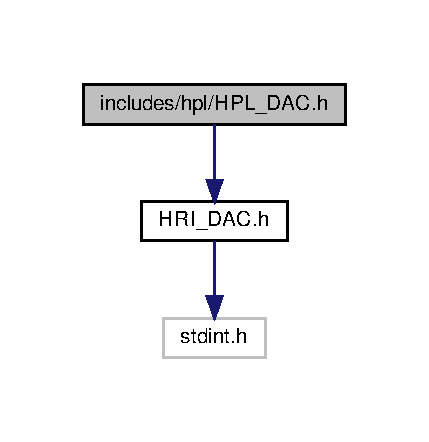
\includegraphics[width=206pt]{HPL__DAC_8h__incl}
\end{center}
\end{figure}
\subsection*{Enumeraciones}
\begin{DoxyCompactItemize}
\item 
\mbox{\Hypertarget{HPL__DAC_8h_af0c73e702603c6124f8c16c4011534aa}\label{HPL__DAC_8h_af0c73e702603c6124f8c16c4011534aa}} 
enum {\bfseries D\+A\+C\+\_\+sel\+\_\+en} \{ {\bfseries D\+A\+C\+\_\+\+S\+E\+L\+\_\+0} = 0, 
{\bfseries D\+A\+C\+\_\+\+S\+E\+L\+\_\+1}
 \}
\item 
\mbox{\Hypertarget{HPL__DAC_8h_ad8bbea38a3e68457c011a40033ccaaf9}\label{HPL__DAC_8h_ad8bbea38a3e68457c011a40033ccaaf9}} 
enum {\bfseries D\+A\+C\+\_\+settling\+\_\+time\+\_\+en} \{ {\bfseries D\+A\+C\+\_\+\+S\+E\+T\+T\+L\+I\+N\+G\+\_\+\+T\+I\+M\+E\+\_\+\+S\+E\+L\+\_\+1\+U\+S\+\_\+\+M\+AX} = 0, 
{\bfseries D\+A\+C\+\_\+\+S\+E\+T\+T\+L\+I\+N\+G\+\_\+\+T\+I\+M\+E\+\_\+\+S\+E\+L\+\_\+2\+\_\+5\+U\+S\+\_\+\+M\+AX}
 \}
\end{DoxyCompactItemize}
\subsection*{Funciones}
\begin{DoxyCompactItemize}
\item 
static void \hyperlink{HPL__DAC_8h_aff942f56ca5445148addbedb009b3717}{D\+A\+C\+\_\+write} (D\+A\+C\+\_\+sel\+\_\+en dac, uint16\+\_\+t new\+\_\+value)
\begin{DoxyCompactList}\small\item\em Actualizacion del valor actual del D\+AC. \end{DoxyCompactList}\item 
static void \hyperlink{HPL__DAC_8h_a434d6125dd07dede66af308283f561e1}{D\+A\+C\+\_\+config\+\_\+settling\+\_\+time} (D\+A\+C\+\_\+sel\+\_\+en dac, D\+A\+C\+\_\+settling\+\_\+time\+\_\+en settling\+\_\+time)
\begin{DoxyCompactList}\small\item\em Configuracion del settling time del D\+AC. \end{DoxyCompactList}\item 
static void \hyperlink{HPL__DAC_8h_ac6695a3e7f2f415a5471ff1ed7cf2c9e}{D\+A\+C\+\_\+enable\+\_\+\+D\+M\+A\+\_\+request} (D\+A\+C\+\_\+sel\+\_\+en dac)
\begin{DoxyCompactList}\small\item\em Habilitar interrupcion de D\+MA cuando el timer tiemoutea. \end{DoxyCompactList}\item 
static void \hyperlink{HPL__DAC_8h_a4003cb71f0fad38416bb7f4fc72d730a}{D\+A\+C\+\_\+disable\+\_\+\+D\+M\+A\+\_\+request} (D\+A\+C\+\_\+sel\+\_\+en dac)
\begin{DoxyCompactList}\small\item\em Inhabilitar interrupcion de D\+MA cuando el timer tiemoutea. \end{DoxyCompactList}\item 
static void \hyperlink{HPL__DAC_8h_a5a17345f5589bf83e76ba51a8b86702a}{D\+A\+C\+\_\+enable\+\_\+double\+\_\+buffer} (D\+A\+C\+\_\+sel\+\_\+en dac)
\begin{DoxyCompactList}\small\item\em Habilitar double buffering. \end{DoxyCompactList}\item 
static void \hyperlink{HPL__DAC_8h_a2b4d91b69ad4020c25fcceb020b6fabf}{D\+A\+C\+\_\+disable\+\_\+double\+\_\+buffer} (D\+A\+C\+\_\+sel\+\_\+en dac)
\begin{DoxyCompactList}\small\item\em Inhabilitar double buffering. \end{DoxyCompactList}\item 
static void \hyperlink{HPL__DAC_8h_a84cfe88364d1b7e71d2e4ab865c18b80}{D\+A\+C\+\_\+enable\+\_\+timer} (D\+A\+C\+\_\+sel\+\_\+en dac)
\begin{DoxyCompactList}\small\item\em Habilitar operacion del timer. \end{DoxyCompactList}\item 
static void \hyperlink{HPL__DAC_8h_af3c12e14a1bce480dea8eed8d9ce3ed5}{D\+A\+C\+\_\+disable\+\_\+timer} (D\+A\+C\+\_\+sel\+\_\+en dac)
\begin{DoxyCompactList}\small\item\em Inhabilitar operacion del timer. \end{DoxyCompactList}\item 
static void \hyperlink{HPL__DAC_8h_ab99836684d3217b2bce37fa5feb90e06}{D\+A\+C\+\_\+enable\+\_\+\+D\+MA} (D\+A\+C\+\_\+sel\+\_\+en dac)
\begin{DoxyCompactList}\small\item\em Habilitar D\+MA request asociada al D\+AC. \end{DoxyCompactList}\item 
static void \hyperlink{HPL__DAC_8h_a4376c8f70d83e9ed03472eeb0838ab26}{D\+A\+C\+\_\+disable\+\_\+\+D\+MA} (D\+A\+C\+\_\+sel\+\_\+en dac)
\begin{DoxyCompactList}\small\item\em Inhabilitar D\+MA request asociada al D\+AC. \end{DoxyCompactList}\item 
static void \hyperlink{HPL__DAC_8h_a686e15db7f41f892c17324959502e82e}{D\+A\+C\+\_\+write\+\_\+reaload\+\_\+value} (D\+A\+C\+\_\+sel\+\_\+en dac, uint16\+\_\+t value)
\begin{DoxyCompactList}\small\item\em Escribir valor a recargar para el timer de D\+MA. \end{DoxyCompactList}\end{DoxyCompactItemize}
\subsection*{Variables}
\begin{DoxyCompactItemize}
\item 
\mbox{\Hypertarget{HPL__DAC_8h_a959fc119f4528130756bf6aaca296427}\label{HPL__DAC_8h_a959fc119f4528130756bf6aaca296427}} 
volatile \hyperlink{HRI__DAC_8h_structDAC__per__t}{D\+A\+C\+\_\+per\+\_\+t} $\ast$const \hyperlink{HPL__DAC_8h_a959fc119f4528130756bf6aaca296427}{D\+AC} \mbox{[}$\,$\mbox{]}
\begin{DoxyCompactList}\small\item\em Perifericos D\+AC. \end{DoxyCompactList}\end{DoxyCompactItemize}


\subsection{Descripción detallada}
Declaraciones a nivel de abstraccion de periferico del D\+AC (L\+P\+C845) 

\begin{DoxyAuthor}{Autor}
Augusto Santini 
\end{DoxyAuthor}
\begin{DoxyDate}{Fecha}
6/2019 
\end{DoxyDate}
\begin{DoxyVersion}{Versión}
1.\+0 
\end{DoxyVersion}


\subsection{Documentación de las funciones}
\mbox{\Hypertarget{HPL__DAC_8h_aff942f56ca5445148addbedb009b3717}\label{HPL__DAC_8h_aff942f56ca5445148addbedb009b3717}} 
\index{H\+P\+L\+\_\+\+D\+A\+C.\+h@{H\+P\+L\+\_\+\+D\+A\+C.\+h}!D\+A\+C\+\_\+write@{D\+A\+C\+\_\+write}}
\index{D\+A\+C\+\_\+write@{D\+A\+C\+\_\+write}!H\+P\+L\+\_\+\+D\+A\+C.\+h@{H\+P\+L\+\_\+\+D\+A\+C.\+h}}
\subsubsection{\texorpdfstring{D\+A\+C\+\_\+write()}{DAC\_write()}}
{\footnotesize\ttfamily static void D\+A\+C\+\_\+write (\begin{DoxyParamCaption}\item[{D\+A\+C\+\_\+sel\+\_\+en}]{dac,  }\item[{uint16\+\_\+t}]{new\+\_\+value }\end{DoxyParamCaption})\hspace{0.3cm}{\ttfamily [inline]}, {\ttfamily [static]}}



Actualizacion del valor actual del D\+AC. 


\begin{DoxyParams}[1]{Parámetros}
\mbox{\tt in}  & {\em dac} & Instancia a actualizar \\
\hline
\mbox{\tt in}  & {\em new\+\_\+value} & Nuevo valor a poner en el D\+AC \\
\hline
\end{DoxyParams}
\mbox{\Hypertarget{HPL__DAC_8h_a434d6125dd07dede66af308283f561e1}\label{HPL__DAC_8h_a434d6125dd07dede66af308283f561e1}} 
\index{H\+P\+L\+\_\+\+D\+A\+C.\+h@{H\+P\+L\+\_\+\+D\+A\+C.\+h}!D\+A\+C\+\_\+config\+\_\+settling\+\_\+time@{D\+A\+C\+\_\+config\+\_\+settling\+\_\+time}}
\index{D\+A\+C\+\_\+config\+\_\+settling\+\_\+time@{D\+A\+C\+\_\+config\+\_\+settling\+\_\+time}!H\+P\+L\+\_\+\+D\+A\+C.\+h@{H\+P\+L\+\_\+\+D\+A\+C.\+h}}
\subsubsection{\texorpdfstring{D\+A\+C\+\_\+config\+\_\+settling\+\_\+time()}{DAC\_config\_settling\_time()}}
{\footnotesize\ttfamily static void D\+A\+C\+\_\+config\+\_\+settling\+\_\+time (\begin{DoxyParamCaption}\item[{D\+A\+C\+\_\+sel\+\_\+en}]{dac,  }\item[{D\+A\+C\+\_\+settling\+\_\+time\+\_\+en}]{settling\+\_\+time }\end{DoxyParamCaption})\hspace{0.3cm}{\ttfamily [inline]}, {\ttfamily [static]}}



Configuracion del settling time del D\+AC. 


\begin{DoxyParams}[1]{Parámetros}
\mbox{\tt in}  & {\em dac} & Instancia a configurar \\
\hline
\mbox{\tt in}  & {\em settling\+\_\+time} & Configuracion deseada \\
\hline
\end{DoxyParams}
\mbox{\Hypertarget{HPL__DAC_8h_ac6695a3e7f2f415a5471ff1ed7cf2c9e}\label{HPL__DAC_8h_ac6695a3e7f2f415a5471ff1ed7cf2c9e}} 
\index{H\+P\+L\+\_\+\+D\+A\+C.\+h@{H\+P\+L\+\_\+\+D\+A\+C.\+h}!D\+A\+C\+\_\+enable\+\_\+\+D\+M\+A\+\_\+request@{D\+A\+C\+\_\+enable\+\_\+\+D\+M\+A\+\_\+request}}
\index{D\+A\+C\+\_\+enable\+\_\+\+D\+M\+A\+\_\+request@{D\+A\+C\+\_\+enable\+\_\+\+D\+M\+A\+\_\+request}!H\+P\+L\+\_\+\+D\+A\+C.\+h@{H\+P\+L\+\_\+\+D\+A\+C.\+h}}
\subsubsection{\texorpdfstring{D\+A\+C\+\_\+enable\+\_\+\+D\+M\+A\+\_\+request()}{DAC\_enable\_DMA\_request()}}
{\footnotesize\ttfamily static void D\+A\+C\+\_\+enable\+\_\+\+D\+M\+A\+\_\+request (\begin{DoxyParamCaption}\item[{D\+A\+C\+\_\+sel\+\_\+en}]{dac }\end{DoxyParamCaption})\hspace{0.3cm}{\ttfamily [inline]}, {\ttfamily [static]}}



Habilitar interrupcion de D\+MA cuando el timer tiemoutea. 


\begin{DoxyParams}[1]{Parámetros}
\mbox{\tt in}  & {\em dac} & Instancia a configurar \\
\hline
\end{DoxyParams}
\mbox{\Hypertarget{HPL__DAC_8h_a4003cb71f0fad38416bb7f4fc72d730a}\label{HPL__DAC_8h_a4003cb71f0fad38416bb7f4fc72d730a}} 
\index{H\+P\+L\+\_\+\+D\+A\+C.\+h@{H\+P\+L\+\_\+\+D\+A\+C.\+h}!D\+A\+C\+\_\+disable\+\_\+\+D\+M\+A\+\_\+request@{D\+A\+C\+\_\+disable\+\_\+\+D\+M\+A\+\_\+request}}
\index{D\+A\+C\+\_\+disable\+\_\+\+D\+M\+A\+\_\+request@{D\+A\+C\+\_\+disable\+\_\+\+D\+M\+A\+\_\+request}!H\+P\+L\+\_\+\+D\+A\+C.\+h@{H\+P\+L\+\_\+\+D\+A\+C.\+h}}
\subsubsection{\texorpdfstring{D\+A\+C\+\_\+disable\+\_\+\+D\+M\+A\+\_\+request()}{DAC\_disable\_DMA\_request()}}
{\footnotesize\ttfamily static void D\+A\+C\+\_\+disable\+\_\+\+D\+M\+A\+\_\+request (\begin{DoxyParamCaption}\item[{D\+A\+C\+\_\+sel\+\_\+en}]{dac }\end{DoxyParamCaption})\hspace{0.3cm}{\ttfamily [inline]}, {\ttfamily [static]}}



Inhabilitar interrupcion de D\+MA cuando el timer tiemoutea. 


\begin{DoxyParams}[1]{Parámetros}
\mbox{\tt in}  & {\em dac} & Instancia a configurar \\
\hline
\end{DoxyParams}
\mbox{\Hypertarget{HPL__DAC_8h_a5a17345f5589bf83e76ba51a8b86702a}\label{HPL__DAC_8h_a5a17345f5589bf83e76ba51a8b86702a}} 
\index{H\+P\+L\+\_\+\+D\+A\+C.\+h@{H\+P\+L\+\_\+\+D\+A\+C.\+h}!D\+A\+C\+\_\+enable\+\_\+double\+\_\+buffer@{D\+A\+C\+\_\+enable\+\_\+double\+\_\+buffer}}
\index{D\+A\+C\+\_\+enable\+\_\+double\+\_\+buffer@{D\+A\+C\+\_\+enable\+\_\+double\+\_\+buffer}!H\+P\+L\+\_\+\+D\+A\+C.\+h@{H\+P\+L\+\_\+\+D\+A\+C.\+h}}
\subsubsection{\texorpdfstring{D\+A\+C\+\_\+enable\+\_\+double\+\_\+buffer()}{DAC\_enable\_double\_buffer()}}
{\footnotesize\ttfamily static void D\+A\+C\+\_\+enable\+\_\+double\+\_\+buffer (\begin{DoxyParamCaption}\item[{D\+A\+C\+\_\+sel\+\_\+en}]{dac }\end{DoxyParamCaption})\hspace{0.3cm}{\ttfamily [inline]}, {\ttfamily [static]}}



Habilitar double buffering. 


\begin{DoxyParams}[1]{Parámetros}
\mbox{\tt in}  & {\em dac} & Instancia a configurar \\
\hline
\end{DoxyParams}
\mbox{\Hypertarget{HPL__DAC_8h_a2b4d91b69ad4020c25fcceb020b6fabf}\label{HPL__DAC_8h_a2b4d91b69ad4020c25fcceb020b6fabf}} 
\index{H\+P\+L\+\_\+\+D\+A\+C.\+h@{H\+P\+L\+\_\+\+D\+A\+C.\+h}!D\+A\+C\+\_\+disable\+\_\+double\+\_\+buffer@{D\+A\+C\+\_\+disable\+\_\+double\+\_\+buffer}}
\index{D\+A\+C\+\_\+disable\+\_\+double\+\_\+buffer@{D\+A\+C\+\_\+disable\+\_\+double\+\_\+buffer}!H\+P\+L\+\_\+\+D\+A\+C.\+h@{H\+P\+L\+\_\+\+D\+A\+C.\+h}}
\subsubsection{\texorpdfstring{D\+A\+C\+\_\+disable\+\_\+double\+\_\+buffer()}{DAC\_disable\_double\_buffer()}}
{\footnotesize\ttfamily static void D\+A\+C\+\_\+disable\+\_\+double\+\_\+buffer (\begin{DoxyParamCaption}\item[{D\+A\+C\+\_\+sel\+\_\+en}]{dac }\end{DoxyParamCaption})\hspace{0.3cm}{\ttfamily [inline]}, {\ttfamily [static]}}



Inhabilitar double buffering. 


\begin{DoxyParams}[1]{Parámetros}
\mbox{\tt in}  & {\em dac} & Instancia a configurar \\
\hline
\end{DoxyParams}
\mbox{\Hypertarget{HPL__DAC_8h_a84cfe88364d1b7e71d2e4ab865c18b80}\label{HPL__DAC_8h_a84cfe88364d1b7e71d2e4ab865c18b80}} 
\index{H\+P\+L\+\_\+\+D\+A\+C.\+h@{H\+P\+L\+\_\+\+D\+A\+C.\+h}!D\+A\+C\+\_\+enable\+\_\+timer@{D\+A\+C\+\_\+enable\+\_\+timer}}
\index{D\+A\+C\+\_\+enable\+\_\+timer@{D\+A\+C\+\_\+enable\+\_\+timer}!H\+P\+L\+\_\+\+D\+A\+C.\+h@{H\+P\+L\+\_\+\+D\+A\+C.\+h}}
\subsubsection{\texorpdfstring{D\+A\+C\+\_\+enable\+\_\+timer()}{DAC\_enable\_timer()}}
{\footnotesize\ttfamily static void D\+A\+C\+\_\+enable\+\_\+timer (\begin{DoxyParamCaption}\item[{D\+A\+C\+\_\+sel\+\_\+en}]{dac }\end{DoxyParamCaption})\hspace{0.3cm}{\ttfamily [inline]}, {\ttfamily [static]}}



Habilitar operacion del timer. 


\begin{DoxyParams}[1]{Parámetros}
\mbox{\tt in}  & {\em dac} & Instancia a configurar \\
\hline
\end{DoxyParams}
\mbox{\Hypertarget{HPL__DAC_8h_af3c12e14a1bce480dea8eed8d9ce3ed5}\label{HPL__DAC_8h_af3c12e14a1bce480dea8eed8d9ce3ed5}} 
\index{H\+P\+L\+\_\+\+D\+A\+C.\+h@{H\+P\+L\+\_\+\+D\+A\+C.\+h}!D\+A\+C\+\_\+disable\+\_\+timer@{D\+A\+C\+\_\+disable\+\_\+timer}}
\index{D\+A\+C\+\_\+disable\+\_\+timer@{D\+A\+C\+\_\+disable\+\_\+timer}!H\+P\+L\+\_\+\+D\+A\+C.\+h@{H\+P\+L\+\_\+\+D\+A\+C.\+h}}
\subsubsection{\texorpdfstring{D\+A\+C\+\_\+disable\+\_\+timer()}{DAC\_disable\_timer()}}
{\footnotesize\ttfamily static void D\+A\+C\+\_\+disable\+\_\+timer (\begin{DoxyParamCaption}\item[{D\+A\+C\+\_\+sel\+\_\+en}]{dac }\end{DoxyParamCaption})\hspace{0.3cm}{\ttfamily [inline]}, {\ttfamily [static]}}



Inhabilitar operacion del timer. 


\begin{DoxyParams}[1]{Parámetros}
\mbox{\tt in}  & {\em dac} & Instancia a configurar \\
\hline
\end{DoxyParams}
\mbox{\Hypertarget{HPL__DAC_8h_ab99836684d3217b2bce37fa5feb90e06}\label{HPL__DAC_8h_ab99836684d3217b2bce37fa5feb90e06}} 
\index{H\+P\+L\+\_\+\+D\+A\+C.\+h@{H\+P\+L\+\_\+\+D\+A\+C.\+h}!D\+A\+C\+\_\+enable\+\_\+\+D\+MA@{D\+A\+C\+\_\+enable\+\_\+\+D\+MA}}
\index{D\+A\+C\+\_\+enable\+\_\+\+D\+MA@{D\+A\+C\+\_\+enable\+\_\+\+D\+MA}!H\+P\+L\+\_\+\+D\+A\+C.\+h@{H\+P\+L\+\_\+\+D\+A\+C.\+h}}
\subsubsection{\texorpdfstring{D\+A\+C\+\_\+enable\+\_\+\+D\+M\+A()}{DAC\_enable\_DMA()}}
{\footnotesize\ttfamily static void D\+A\+C\+\_\+enable\+\_\+\+D\+MA (\begin{DoxyParamCaption}\item[{D\+A\+C\+\_\+sel\+\_\+en}]{dac }\end{DoxyParamCaption})\hspace{0.3cm}{\ttfamily [inline]}, {\ttfamily [static]}}



Habilitar D\+MA request asociada al D\+AC. 


\begin{DoxyParams}[1]{Parámetros}
\mbox{\tt in}  & {\em dac} & Instancia a configurar \\
\hline
\end{DoxyParams}
\mbox{\Hypertarget{HPL__DAC_8h_a4376c8f70d83e9ed03472eeb0838ab26}\label{HPL__DAC_8h_a4376c8f70d83e9ed03472eeb0838ab26}} 
\index{H\+P\+L\+\_\+\+D\+A\+C.\+h@{H\+P\+L\+\_\+\+D\+A\+C.\+h}!D\+A\+C\+\_\+disable\+\_\+\+D\+MA@{D\+A\+C\+\_\+disable\+\_\+\+D\+MA}}
\index{D\+A\+C\+\_\+disable\+\_\+\+D\+MA@{D\+A\+C\+\_\+disable\+\_\+\+D\+MA}!H\+P\+L\+\_\+\+D\+A\+C.\+h@{H\+P\+L\+\_\+\+D\+A\+C.\+h}}
\subsubsection{\texorpdfstring{D\+A\+C\+\_\+disable\+\_\+\+D\+M\+A()}{DAC\_disable\_DMA()}}
{\footnotesize\ttfamily static void D\+A\+C\+\_\+disable\+\_\+\+D\+MA (\begin{DoxyParamCaption}\item[{D\+A\+C\+\_\+sel\+\_\+en}]{dac }\end{DoxyParamCaption})\hspace{0.3cm}{\ttfamily [inline]}, {\ttfamily [static]}}



Inhabilitar D\+MA request asociada al D\+AC. 


\begin{DoxyParams}[1]{Parámetros}
\mbox{\tt in}  & {\em dac} & Instancia a configurar \\
\hline
\end{DoxyParams}
\mbox{\Hypertarget{HPL__DAC_8h_a686e15db7f41f892c17324959502e82e}\label{HPL__DAC_8h_a686e15db7f41f892c17324959502e82e}} 
\index{H\+P\+L\+\_\+\+D\+A\+C.\+h@{H\+P\+L\+\_\+\+D\+A\+C.\+h}!D\+A\+C\+\_\+write\+\_\+reaload\+\_\+value@{D\+A\+C\+\_\+write\+\_\+reaload\+\_\+value}}
\index{D\+A\+C\+\_\+write\+\_\+reaload\+\_\+value@{D\+A\+C\+\_\+write\+\_\+reaload\+\_\+value}!H\+P\+L\+\_\+\+D\+A\+C.\+h@{H\+P\+L\+\_\+\+D\+A\+C.\+h}}
\subsubsection{\texorpdfstring{D\+A\+C\+\_\+write\+\_\+reaload\+\_\+value()}{DAC\_write\_reaload\_value()}}
{\footnotesize\ttfamily static void D\+A\+C\+\_\+write\+\_\+reaload\+\_\+value (\begin{DoxyParamCaption}\item[{D\+A\+C\+\_\+sel\+\_\+en}]{dac,  }\item[{uint16\+\_\+t}]{value }\end{DoxyParamCaption})\hspace{0.3cm}{\ttfamily [inline]}, {\ttfamily [static]}}



Escribir valor a recargar para el timer de D\+MA. 


\begin{DoxyParams}[1]{Parámetros}
\mbox{\tt in}  & {\em dac} & Instancia a configurar \\
\hline
\mbox{\tt in}  & {\em value} & Valor deseado \\
\hline
\end{DoxyParams}

\hypertarget{HPL__GPIO_8h}{}\section{Referencia del Archivo includes/hpl/\+H\+P\+L\+\_\+\+G\+P\+IO.h}
\label{HPL__GPIO_8h}\index{includes/hpl/\+H\+P\+L\+\_\+\+G\+P\+I\+O.\+h@{includes/hpl/\+H\+P\+L\+\_\+\+G\+P\+I\+O.\+h}}


Declaraciones a nivel de abstraccion de periferico del G\+P\+IO (L\+P\+C845)  


{\ttfamily \#include $<$H\+R\+I\+\_\+\+G\+P\+I\+O.\+h$>$}\newline
Dependencia gráfica adjunta para H\+P\+L\+\_\+\+G\+P\+I\+O.\+h\+:
\nopagebreak
\begin{figure}[H]
\begin{center}
\leavevmode
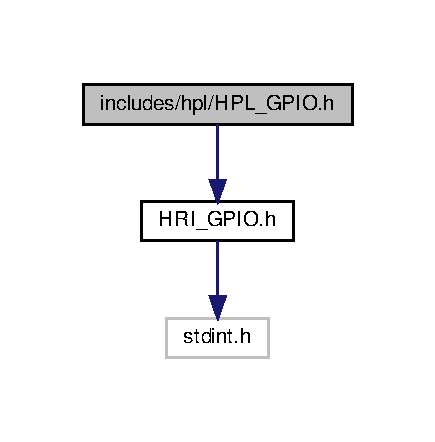
\includegraphics[width=209pt]{d0/d86/HPL__GPIO_8h__incl}
\end{center}
\end{figure}
Gráfico de los archivos que directa o indirectamente incluyen a este archivo\+:\nopagebreak
\begin{figure}[H]
\begin{center}
\leavevmode
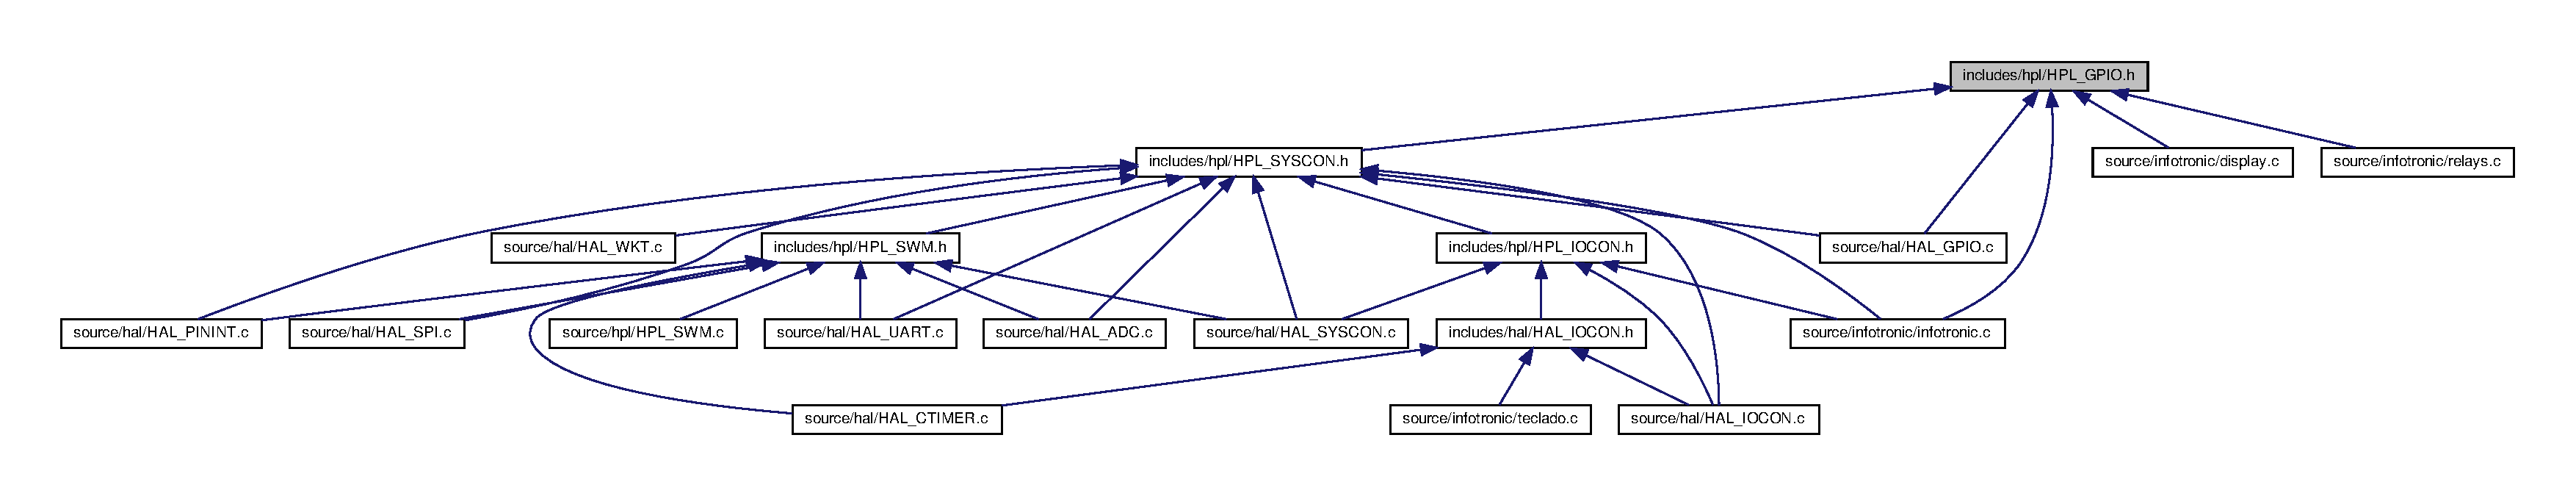
\includegraphics[width=350pt]{d7/d7b/HPL__GPIO_8h__dep__incl}
\end{center}
\end{figure}
\subsection*{Enumeraciones}
\begin{DoxyCompactItemize}
\item 
\mbox{\Hypertarget{HPL__GPIO_8h_aa8a5f03feb423b58c240c97d4d01349b}\label{HPL__GPIO_8h_aa8a5f03feb423b58c240c97d4d01349b}} 
enum {\bfseries G\+P\+I\+O\+\_\+dir\+\_\+en} \{ {\bfseries G\+P\+I\+O\+\_\+\+D\+I\+R\+\_\+\+I\+N\+P\+UT} = 0, 
{\bfseries G\+P\+I\+O\+\_\+\+D\+I\+R\+\_\+\+O\+U\+T\+P\+UT}
 \}
\item 
\mbox{\Hypertarget{HPL__GPIO_8h_ae5f6b02ed6c36507322c013a64408f4c}\label{HPL__GPIO_8h_ae5f6b02ed6c36507322c013a64408f4c}} 
enum {\bfseries G\+P\+I\+O\+\_\+port\+\_\+en} \{ {\bfseries G\+P\+I\+O\+\_\+\+P\+O\+R\+T\+\_\+0} = 0, 
{\bfseries G\+P\+I\+O\+\_\+\+P\+O\+R\+T\+\_\+1}
 \}
\item 
\mbox{\Hypertarget{HPL__GPIO_8h_aa0fafee8b50ae50a7b6c6ce86b6214fd}\label{HPL__GPIO_8h_aa0fafee8b50ae50a7b6c6ce86b6214fd}} 
enum {\bfseries G\+P\+I\+O\+\_\+portpin\+\_\+en} \{ \newline
{\bfseries G\+P\+I\+O\+\_\+\+P\+O\+R\+T\+P\+I\+N\+\_\+0\+\_\+0} = 0, 
{\bfseries G\+P\+I\+O\+\_\+\+P\+O\+R\+T\+P\+I\+N\+\_\+0\+\_\+1}, 
{\bfseries G\+P\+I\+O\+\_\+\+P\+O\+R\+T\+P\+I\+N\+\_\+0\+\_\+2}, 
{\bfseries G\+P\+I\+O\+\_\+\+P\+O\+R\+T\+P\+I\+N\+\_\+0\+\_\+3}, 
\newline
{\bfseries G\+P\+I\+O\+\_\+\+P\+O\+R\+T\+P\+I\+N\+\_\+0\+\_\+4}, 
{\bfseries G\+P\+I\+O\+\_\+\+P\+O\+R\+T\+P\+I\+N\+\_\+0\+\_\+5}, 
{\bfseries G\+P\+I\+O\+\_\+\+P\+O\+R\+T\+P\+I\+N\+\_\+0\+\_\+6}, 
{\bfseries G\+P\+I\+O\+\_\+\+P\+O\+R\+T\+P\+I\+N\+\_\+0\+\_\+7}, 
\newline
{\bfseries G\+P\+I\+O\+\_\+\+P\+O\+R\+T\+P\+I\+N\+\_\+0\+\_\+8}, 
{\bfseries G\+P\+I\+O\+\_\+\+P\+O\+R\+T\+P\+I\+N\+\_\+0\+\_\+9}, 
{\bfseries G\+P\+I\+O\+\_\+\+P\+O\+R\+T\+P\+I\+N\+\_\+0\+\_\+10}, 
{\bfseries G\+P\+I\+O\+\_\+\+P\+O\+R\+T\+P\+I\+N\+\_\+0\+\_\+11}, 
\newline
{\bfseries G\+P\+I\+O\+\_\+\+P\+O\+R\+T\+P\+I\+N\+\_\+0\+\_\+12}, 
{\bfseries G\+P\+I\+O\+\_\+\+P\+O\+R\+T\+P\+I\+N\+\_\+0\+\_\+13}, 
{\bfseries G\+P\+I\+O\+\_\+\+P\+O\+R\+T\+P\+I\+N\+\_\+0\+\_\+14}, 
{\bfseries G\+P\+I\+O\+\_\+\+P\+O\+R\+T\+P\+I\+N\+\_\+0\+\_\+15}, 
\newline
{\bfseries G\+P\+I\+O\+\_\+\+P\+O\+R\+T\+P\+I\+N\+\_\+0\+\_\+16}, 
{\bfseries G\+P\+I\+O\+\_\+\+P\+O\+R\+T\+P\+I\+N\+\_\+0\+\_\+17}, 
{\bfseries G\+P\+I\+O\+\_\+\+P\+O\+R\+T\+P\+I\+N\+\_\+0\+\_\+18}, 
{\bfseries G\+P\+I\+O\+\_\+\+P\+O\+R\+T\+P\+I\+N\+\_\+0\+\_\+19}, 
\newline
{\bfseries G\+P\+I\+O\+\_\+\+P\+O\+R\+T\+P\+I\+N\+\_\+0\+\_\+20}, 
{\bfseries G\+P\+I\+O\+\_\+\+P\+O\+R\+T\+P\+I\+N\+\_\+0\+\_\+21}, 
{\bfseries G\+P\+I\+O\+\_\+\+P\+O\+R\+T\+P\+I\+N\+\_\+0\+\_\+22}, 
{\bfseries G\+P\+I\+O\+\_\+\+P\+O\+R\+T\+P\+I\+N\+\_\+0\+\_\+23}, 
\newline
{\bfseries G\+P\+I\+O\+\_\+\+P\+O\+R\+T\+P\+I\+N\+\_\+0\+\_\+24}, 
{\bfseries G\+P\+I\+O\+\_\+\+P\+O\+R\+T\+P\+I\+N\+\_\+0\+\_\+25}, 
{\bfseries G\+P\+I\+O\+\_\+\+P\+O\+R\+T\+P\+I\+N\+\_\+0\+\_\+26}, 
{\bfseries G\+P\+I\+O\+\_\+\+P\+O\+R\+T\+P\+I\+N\+\_\+0\+\_\+27}, 
\newline
{\bfseries G\+P\+I\+O\+\_\+\+P\+O\+R\+T\+P\+I\+N\+\_\+0\+\_\+28}, 
{\bfseries G\+P\+I\+O\+\_\+\+P\+O\+R\+T\+P\+I\+N\+\_\+0\+\_\+29}, 
{\bfseries G\+P\+I\+O\+\_\+\+P\+O\+R\+T\+P\+I\+N\+\_\+0\+\_\+30}, 
{\bfseries G\+P\+I\+O\+\_\+\+P\+O\+R\+T\+P\+I\+N\+\_\+0\+\_\+31}, 
\newline
{\bfseries G\+P\+I\+O\+\_\+\+P\+O\+R\+T\+P\+I\+N\+\_\+1\+\_\+0}, 
{\bfseries G\+P\+I\+O\+\_\+\+P\+O\+R\+T\+P\+I\+N\+\_\+1\+\_\+1}, 
{\bfseries G\+P\+I\+O\+\_\+\+P\+O\+R\+T\+P\+I\+N\+\_\+1\+\_\+2}, 
{\bfseries G\+P\+I\+O\+\_\+\+P\+O\+R\+T\+P\+I\+N\+\_\+1\+\_\+3}, 
\newline
{\bfseries G\+P\+I\+O\+\_\+\+P\+O\+R\+T\+P\+I\+N\+\_\+1\+\_\+4}, 
{\bfseries G\+P\+I\+O\+\_\+\+P\+O\+R\+T\+P\+I\+N\+\_\+1\+\_\+5}, 
{\bfseries G\+P\+I\+O\+\_\+\+P\+O\+R\+T\+P\+I\+N\+\_\+1\+\_\+6}, 
{\bfseries G\+P\+I\+O\+\_\+\+P\+O\+R\+T\+P\+I\+N\+\_\+1\+\_\+7}, 
\newline
{\bfseries G\+P\+I\+O\+\_\+\+P\+O\+R\+T\+P\+I\+N\+\_\+1\+\_\+8}, 
{\bfseries G\+P\+I\+O\+\_\+\+P\+O\+R\+T\+P\+I\+N\+\_\+1\+\_\+9}, 
{\bfseries G\+P\+I\+O\+\_\+\+P\+O\+R\+T\+P\+I\+N\+\_\+1\+\_\+10}, 
{\bfseries G\+P\+I\+O\+\_\+\+P\+O\+R\+T\+P\+I\+N\+\_\+1\+\_\+11}, 
\newline
{\bfseries G\+P\+I\+O\+\_\+\+P\+O\+R\+T\+P\+I\+N\+\_\+1\+\_\+12}, 
{\bfseries G\+P\+I\+O\+\_\+\+P\+O\+R\+T\+P\+I\+N\+\_\+1\+\_\+13}, 
{\bfseries G\+P\+I\+O\+\_\+\+P\+O\+R\+T\+P\+I\+N\+\_\+1\+\_\+14}, 
{\bfseries G\+P\+I\+O\+\_\+\+P\+O\+R\+T\+P\+I\+N\+\_\+1\+\_\+15}, 
\newline
{\bfseries G\+P\+I\+O\+\_\+\+P\+O\+R\+T\+P\+I\+N\+\_\+1\+\_\+16}, 
{\bfseries G\+P\+I\+O\+\_\+\+P\+O\+R\+T\+P\+I\+N\+\_\+1\+\_\+17}, 
{\bfseries G\+P\+I\+O\+\_\+\+P\+O\+R\+T\+P\+I\+N\+\_\+1\+\_\+18}, 
{\bfseries G\+P\+I\+O\+\_\+\+P\+O\+R\+T\+P\+I\+N\+\_\+1\+\_\+19}, 
\newline
{\bfseries G\+P\+I\+O\+\_\+\+P\+O\+R\+T\+P\+I\+N\+\_\+1\+\_\+20}, 
{\bfseries G\+P\+I\+O\+\_\+\+P\+O\+R\+T\+P\+I\+N\+\_\+1\+\_\+21}
 \}
\end{DoxyCompactItemize}
\subsection*{Funciones}
\begin{DoxyCompactItemize}
\item 
static uint8\+\_\+t \hyperlink{HPL__GPIO_8h_a267ed6e1418eeb6195b5d6b4ac056fd2}{G\+P\+I\+O\+\_\+read\+\_\+port\+\_\+byte} (G\+P\+I\+O\+\_\+portpin\+\_\+en portpin)
\begin{DoxyCompactList}\small\item\em Leer estado del pin absoluto (sin importar mascaras ni funcion alternativa) \end{DoxyCompactList}\item 
static void \hyperlink{HPL__GPIO_8h_a4f755711238776b072e1bf3488de07ec}{G\+P\+I\+O\+\_\+write\+\_\+port\+\_\+byte} (G\+P\+I\+O\+\_\+portpin\+\_\+en portpin, uint8\+\_\+t value)
\begin{DoxyCompactList}\small\item\em Escribir estado del pin absoluto (sin importar mascaras ni funcion alternativa) \end{DoxyCompactList}\item 
static uint8\+\_\+t \hyperlink{HPL__GPIO_8h_ada3afe036dc9ffb22914011692c8bb0f}{G\+P\+I\+O\+\_\+read\+\_\+port\+\_\+word} (G\+P\+I\+O\+\_\+portpin\+\_\+en portpin)
\begin{DoxyCompactList}\small\item\em Leer estado del pin absoluto (sin importar mascaras ni funcion alternativa) \end{DoxyCompactList}\item 
static void \hyperlink{HPL__GPIO_8h_aca5019b34a67a3c5b49e3b5e36ad0b4b}{G\+P\+I\+O\+\_\+write\+\_\+port\+\_\+word} (G\+P\+I\+O\+\_\+portpin\+\_\+en portpin, uint8\+\_\+t value)
\begin{DoxyCompactList}\small\item\em Escribir estado del pin absoluto (sin importar mascaras ni funcion alternativa) \end{DoxyCompactList}\item 
static uint32\+\_\+t \hyperlink{HPL__GPIO_8h_a42362e26a5f6f3ec958493d59b7d01f3}{G\+P\+I\+O\+\_\+read\+\_\+dir} (G\+P\+I\+O\+\_\+port\+\_\+en port)
\begin{DoxyCompactList}\small\item\em Leer registro de direccion. \end{DoxyCompactList}\item 
static void \hyperlink{HPL__GPIO_8h_a152db9639dd4194c7df2b7bbbe251770}{G\+P\+I\+O\+\_\+write\+\_\+dir} (G\+P\+I\+O\+\_\+port\+\_\+en port, uint32\+\_\+t value)
\begin{DoxyCompactList}\small\item\em Escribir registro de direccion. \end{DoxyCompactList}\item 
static uint32\+\_\+t \hyperlink{HPL__GPIO_8h_af9d6f53771444f37534abbdcc4c0c1a7}{G\+P\+I\+O\+\_\+read\+\_\+mask} (G\+P\+I\+O\+\_\+port\+\_\+en port)
\begin{DoxyCompactList}\small\item\em Leer registro de mascara. \end{DoxyCompactList}\item 
static void \hyperlink{HPL__GPIO_8h_af5b1053f7582eee056f34678a65299bd}{G\+P\+I\+O\+\_\+write\+\_\+mask} (G\+P\+I\+O\+\_\+port\+\_\+en port, uint32\+\_\+t value)
\begin{DoxyCompactList}\small\item\em Escribir registro de mascara. \end{DoxyCompactList}\item 
static uint32\+\_\+t \hyperlink{HPL__GPIO_8h_ac632c0f75c4423c5900d3e4f421a7de8}{G\+P\+I\+O\+\_\+read\+\_\+portpin} (G\+P\+I\+O\+\_\+port\+\_\+en port)
\begin{DoxyCompactList}\small\item\em Leer registro de puerto/pin. \end{DoxyCompactList}\item 
static void \hyperlink{HPL__GPIO_8h_a68e1b812428ac21ac61579e2284805e4}{G\+P\+I\+O\+\_\+write\+\_\+portpin} (G\+P\+I\+O\+\_\+port\+\_\+en port, uint32\+\_\+t value)
\begin{DoxyCompactList}\small\item\em Escribir registro de puerto/pin. \end{DoxyCompactList}\item 
static uint32\+\_\+t \hyperlink{HPL__GPIO_8h_ad2e00803fe1f021aa37d216fb91f3409}{G\+P\+I\+O\+\_\+read\+\_\+masked\+\_\+portpin} (G\+P\+I\+O\+\_\+port\+\_\+en port)
\begin{DoxyCompactList}\small\item\em Leer registro de puerto/pin enmascarado. \end{DoxyCompactList}\item 
static void \hyperlink{HPL__GPIO_8h_a3e9d14fe2bf5f285602f12180a0c662b}{G\+P\+I\+O\+\_\+write\+\_\+masked\+\_\+portpin} (G\+P\+I\+O\+\_\+port\+\_\+en port, uint32\+\_\+t value)
\begin{DoxyCompactList}\small\item\em Escribir registro de puerto/pin enmascarado. \end{DoxyCompactList}\item 
static void \hyperlink{HPL__GPIO_8h_aad6ffff0b47580a7dc37715efc23e4cb}{G\+P\+I\+O\+\_\+write\+\_\+set} (G\+P\+I\+O\+\_\+port\+\_\+en port, uint32\+\_\+t value)
\begin{DoxyCompactList}\small\item\em Escribir registro de set. \end{DoxyCompactList}\item 
static void \hyperlink{HPL__GPIO_8h_a0922b5124761aeb3289ad91364a7c274}{G\+P\+I\+O\+\_\+write\+\_\+clear} (G\+P\+I\+O\+\_\+port\+\_\+en port, uint32\+\_\+t value)
\begin{DoxyCompactList}\small\item\em Escribir registro de clear. \end{DoxyCompactList}\item 
static void \hyperlink{HPL__GPIO_8h_a858ca89771d84f54f30363f49d061a98}{G\+P\+I\+O\+\_\+write\+\_\+toggle} (G\+P\+I\+O\+\_\+port\+\_\+en port, uint32\+\_\+t value)
\begin{DoxyCompactList}\small\item\em Escribir registro de toggle. \end{DoxyCompactList}\item 
static void \hyperlink{HPL__GPIO_8h_a2ac4da95b704e73e7521bdf5ae8074b7}{G\+P\+I\+O\+\_\+write\+\_\+dir\+\_\+set} (G\+P\+I\+O\+\_\+port\+\_\+en port, uint32\+\_\+t value)
\begin{DoxyCompactList}\small\item\em Escribir registro de direction set. \end{DoxyCompactList}\item 
static void \hyperlink{HPL__GPIO_8h_a3ae4f56ad6fbc751590fe2fe59828209}{G\+P\+I\+O\+\_\+write\+\_\+dir\+\_\+clear} (G\+P\+I\+O\+\_\+port\+\_\+en port, uint32\+\_\+t value)
\begin{DoxyCompactList}\small\item\em Escribir registro de direction clear. \end{DoxyCompactList}\item 
static void \hyperlink{HPL__GPIO_8h_a36e0a677fb97a34251b39c7a213944f1}{G\+P\+I\+O\+\_\+write\+\_\+dir\+\_\+toggle} (G\+P\+I\+O\+\_\+port\+\_\+en port, uint32\+\_\+t value)
\begin{DoxyCompactList}\small\item\em Escribir registro de direction toggle. \end{DoxyCompactList}\end{DoxyCompactItemize}
\subsection*{Variables}
\begin{DoxyCompactItemize}
\item 
\mbox{\Hypertarget{HPL__GPIO_8h_a0590bc531d55b228a07b0da230fcf86c}\label{HPL__GPIO_8h_a0590bc531d55b228a07b0da230fcf86c}} 
volatile \hyperlink{HRI__GPIO_8h_dd/d45/structGPIO__per__t}{G\+P\+I\+O\+\_\+per\+\_\+t} $\ast$const \hyperlink{HPL__GPIO_8h_a0590bc531d55b228a07b0da230fcf86c}{G\+P\+IO}
\begin{DoxyCompactList}\small\item\em Periferico G\+P\+IO. \end{DoxyCompactList}\end{DoxyCompactItemize}


\subsection{Descripción detallada}
Declaraciones a nivel de abstraccion de periferico del G\+P\+IO (L\+P\+C845) 

\begin{DoxyAuthor}{Autor}
Augusto Santini 
\end{DoxyAuthor}
\begin{DoxyDate}{Fecha}
6/2019 
\end{DoxyDate}
\begin{DoxyVersion}{Versión}
1.\+0 
\end{DoxyVersion}


\subsection{Documentación de las funciones}
\mbox{\Hypertarget{HPL__GPIO_8h_a267ed6e1418eeb6195b5d6b4ac056fd2}\label{HPL__GPIO_8h_a267ed6e1418eeb6195b5d6b4ac056fd2}} 
\index{H\+P\+L\+\_\+\+G\+P\+I\+O.\+h@{H\+P\+L\+\_\+\+G\+P\+I\+O.\+h}!G\+P\+I\+O\+\_\+read\+\_\+port\+\_\+byte@{G\+P\+I\+O\+\_\+read\+\_\+port\+\_\+byte}}
\index{G\+P\+I\+O\+\_\+read\+\_\+port\+\_\+byte@{G\+P\+I\+O\+\_\+read\+\_\+port\+\_\+byte}!H\+P\+L\+\_\+\+G\+P\+I\+O.\+h@{H\+P\+L\+\_\+\+G\+P\+I\+O.\+h}}
\subsubsection{\texorpdfstring{G\+P\+I\+O\+\_\+read\+\_\+port\+\_\+byte()}{GPIO\_read\_port\_byte()}}
{\footnotesize\ttfamily static uint8\+\_\+t G\+P\+I\+O\+\_\+read\+\_\+port\+\_\+byte (\begin{DoxyParamCaption}\item[{G\+P\+I\+O\+\_\+portpin\+\_\+en}]{portpin }\end{DoxyParamCaption})\hspace{0.3cm}{\ttfamily [inline]}, {\ttfamily [static]}}



Leer estado del pin absoluto (sin importar mascaras ni funcion alternativa) 


\begin{DoxyParams}[1]{Parámetros}
\mbox{\tt in}  & {\em portpin} & Numero de port/pin a consultar \\
\hline
\end{DoxyParams}
\begin{DoxyReturn}{Devuelve}
Estado del pin absoluto 
\end{DoxyReturn}
\mbox{\Hypertarget{HPL__GPIO_8h_a4f755711238776b072e1bf3488de07ec}\label{HPL__GPIO_8h_a4f755711238776b072e1bf3488de07ec}} 
\index{H\+P\+L\+\_\+\+G\+P\+I\+O.\+h@{H\+P\+L\+\_\+\+G\+P\+I\+O.\+h}!G\+P\+I\+O\+\_\+write\+\_\+port\+\_\+byte@{G\+P\+I\+O\+\_\+write\+\_\+port\+\_\+byte}}
\index{G\+P\+I\+O\+\_\+write\+\_\+port\+\_\+byte@{G\+P\+I\+O\+\_\+write\+\_\+port\+\_\+byte}!H\+P\+L\+\_\+\+G\+P\+I\+O.\+h@{H\+P\+L\+\_\+\+G\+P\+I\+O.\+h}}
\subsubsection{\texorpdfstring{G\+P\+I\+O\+\_\+write\+\_\+port\+\_\+byte()}{GPIO\_write\_port\_byte()}}
{\footnotesize\ttfamily static void G\+P\+I\+O\+\_\+write\+\_\+port\+\_\+byte (\begin{DoxyParamCaption}\item[{G\+P\+I\+O\+\_\+portpin\+\_\+en}]{portpin,  }\item[{uint8\+\_\+t}]{value }\end{DoxyParamCaption})\hspace{0.3cm}{\ttfamily [inline]}, {\ttfamily [static]}}



Escribir estado del pin absoluto (sin importar mascaras ni funcion alternativa) 


\begin{DoxyParams}[1]{Parámetros}
\mbox{\tt in}  & {\em portpin} & Numero de port/pin a escribir \\
\hline
\mbox{\tt in}  & {\em value} & Valor a escribir \\
\hline
\end{DoxyParams}
\mbox{\Hypertarget{HPL__GPIO_8h_ada3afe036dc9ffb22914011692c8bb0f}\label{HPL__GPIO_8h_ada3afe036dc9ffb22914011692c8bb0f}} 
\index{H\+P\+L\+\_\+\+G\+P\+I\+O.\+h@{H\+P\+L\+\_\+\+G\+P\+I\+O.\+h}!G\+P\+I\+O\+\_\+read\+\_\+port\+\_\+word@{G\+P\+I\+O\+\_\+read\+\_\+port\+\_\+word}}
\index{G\+P\+I\+O\+\_\+read\+\_\+port\+\_\+word@{G\+P\+I\+O\+\_\+read\+\_\+port\+\_\+word}!H\+P\+L\+\_\+\+G\+P\+I\+O.\+h@{H\+P\+L\+\_\+\+G\+P\+I\+O.\+h}}
\subsubsection{\texorpdfstring{G\+P\+I\+O\+\_\+read\+\_\+port\+\_\+word()}{GPIO\_read\_port\_word()}}
{\footnotesize\ttfamily static uint8\+\_\+t G\+P\+I\+O\+\_\+read\+\_\+port\+\_\+word (\begin{DoxyParamCaption}\item[{G\+P\+I\+O\+\_\+portpin\+\_\+en}]{portpin }\end{DoxyParamCaption})\hspace{0.3cm}{\ttfamily [inline]}, {\ttfamily [static]}}



Leer estado del pin absoluto (sin importar mascaras ni funcion alternativa) 


\begin{DoxyParams}[1]{Parámetros}
\mbox{\tt in}  & {\em portpin} & Numero de port/pin a consultar \\
\hline
\end{DoxyParams}
\begin{DoxyReturn}{Devuelve}
Estado del pin absoluto 
\end{DoxyReturn}
\mbox{\Hypertarget{HPL__GPIO_8h_aca5019b34a67a3c5b49e3b5e36ad0b4b}\label{HPL__GPIO_8h_aca5019b34a67a3c5b49e3b5e36ad0b4b}} 
\index{H\+P\+L\+\_\+\+G\+P\+I\+O.\+h@{H\+P\+L\+\_\+\+G\+P\+I\+O.\+h}!G\+P\+I\+O\+\_\+write\+\_\+port\+\_\+word@{G\+P\+I\+O\+\_\+write\+\_\+port\+\_\+word}}
\index{G\+P\+I\+O\+\_\+write\+\_\+port\+\_\+word@{G\+P\+I\+O\+\_\+write\+\_\+port\+\_\+word}!H\+P\+L\+\_\+\+G\+P\+I\+O.\+h@{H\+P\+L\+\_\+\+G\+P\+I\+O.\+h}}
\subsubsection{\texorpdfstring{G\+P\+I\+O\+\_\+write\+\_\+port\+\_\+word()}{GPIO\_write\_port\_word()}}
{\footnotesize\ttfamily static void G\+P\+I\+O\+\_\+write\+\_\+port\+\_\+word (\begin{DoxyParamCaption}\item[{G\+P\+I\+O\+\_\+portpin\+\_\+en}]{portpin,  }\item[{uint8\+\_\+t}]{value }\end{DoxyParamCaption})\hspace{0.3cm}{\ttfamily [inline]}, {\ttfamily [static]}}



Escribir estado del pin absoluto (sin importar mascaras ni funcion alternativa) 


\begin{DoxyParams}[1]{Parámetros}
\mbox{\tt in}  & {\em portpin} & Numero de port/pin a escribir \\
\hline
\mbox{\tt in}  & {\em value} & Valor a escribir \\
\hline
\end{DoxyParams}
\mbox{\Hypertarget{HPL__GPIO_8h_a42362e26a5f6f3ec958493d59b7d01f3}\label{HPL__GPIO_8h_a42362e26a5f6f3ec958493d59b7d01f3}} 
\index{H\+P\+L\+\_\+\+G\+P\+I\+O.\+h@{H\+P\+L\+\_\+\+G\+P\+I\+O.\+h}!G\+P\+I\+O\+\_\+read\+\_\+dir@{G\+P\+I\+O\+\_\+read\+\_\+dir}}
\index{G\+P\+I\+O\+\_\+read\+\_\+dir@{G\+P\+I\+O\+\_\+read\+\_\+dir}!H\+P\+L\+\_\+\+G\+P\+I\+O.\+h@{H\+P\+L\+\_\+\+G\+P\+I\+O.\+h}}
\subsubsection{\texorpdfstring{G\+P\+I\+O\+\_\+read\+\_\+dir()}{GPIO\_read\_dir()}}
{\footnotesize\ttfamily static uint32\+\_\+t G\+P\+I\+O\+\_\+read\+\_\+dir (\begin{DoxyParamCaption}\item[{G\+P\+I\+O\+\_\+port\+\_\+en}]{port }\end{DoxyParamCaption})\hspace{0.3cm}{\ttfamily [inline]}, {\ttfamily [static]}}



Leer registro de direccion. 


\begin{DoxyParams}[1]{Parámetros}
\mbox{\tt in}  & {\em port} & Numero de puerto a consultar \\
\hline
\end{DoxyParams}
\begin{DoxyReturn}{Devuelve}
Valor del registro 
\end{DoxyReturn}
\mbox{\Hypertarget{HPL__GPIO_8h_a152db9639dd4194c7df2b7bbbe251770}\label{HPL__GPIO_8h_a152db9639dd4194c7df2b7bbbe251770}} 
\index{H\+P\+L\+\_\+\+G\+P\+I\+O.\+h@{H\+P\+L\+\_\+\+G\+P\+I\+O.\+h}!G\+P\+I\+O\+\_\+write\+\_\+dir@{G\+P\+I\+O\+\_\+write\+\_\+dir}}
\index{G\+P\+I\+O\+\_\+write\+\_\+dir@{G\+P\+I\+O\+\_\+write\+\_\+dir}!H\+P\+L\+\_\+\+G\+P\+I\+O.\+h@{H\+P\+L\+\_\+\+G\+P\+I\+O.\+h}}
\subsubsection{\texorpdfstring{G\+P\+I\+O\+\_\+write\+\_\+dir()}{GPIO\_write\_dir()}}
{\footnotesize\ttfamily static void G\+P\+I\+O\+\_\+write\+\_\+dir (\begin{DoxyParamCaption}\item[{G\+P\+I\+O\+\_\+port\+\_\+en}]{port,  }\item[{uint32\+\_\+t}]{value }\end{DoxyParamCaption})\hspace{0.3cm}{\ttfamily [inline]}, {\ttfamily [static]}}



Escribir registro de direccion. 


\begin{DoxyParams}[1]{Parámetros}
\mbox{\tt in}  & {\em port} & Numero de puerto a configurar \\
\hline
\mbox{\tt in}  & {\em value} & Valor deseado \\
\hline
\end{DoxyParams}
\mbox{\Hypertarget{HPL__GPIO_8h_af9d6f53771444f37534abbdcc4c0c1a7}\label{HPL__GPIO_8h_af9d6f53771444f37534abbdcc4c0c1a7}} 
\index{H\+P\+L\+\_\+\+G\+P\+I\+O.\+h@{H\+P\+L\+\_\+\+G\+P\+I\+O.\+h}!G\+P\+I\+O\+\_\+read\+\_\+mask@{G\+P\+I\+O\+\_\+read\+\_\+mask}}
\index{G\+P\+I\+O\+\_\+read\+\_\+mask@{G\+P\+I\+O\+\_\+read\+\_\+mask}!H\+P\+L\+\_\+\+G\+P\+I\+O.\+h@{H\+P\+L\+\_\+\+G\+P\+I\+O.\+h}}
\subsubsection{\texorpdfstring{G\+P\+I\+O\+\_\+read\+\_\+mask()}{GPIO\_read\_mask()}}
{\footnotesize\ttfamily static uint32\+\_\+t G\+P\+I\+O\+\_\+read\+\_\+mask (\begin{DoxyParamCaption}\item[{G\+P\+I\+O\+\_\+port\+\_\+en}]{port }\end{DoxyParamCaption})\hspace{0.3cm}{\ttfamily [inline]}, {\ttfamily [static]}}



Leer registro de mascara. 


\begin{DoxyParams}[1]{Parámetros}
\mbox{\tt in}  & {\em port} & Numero de puerto a consultar \\
\hline
\end{DoxyParams}
\begin{DoxyReturn}{Devuelve}
Valor del registro 
\end{DoxyReturn}
\mbox{\Hypertarget{HPL__GPIO_8h_af5b1053f7582eee056f34678a65299bd}\label{HPL__GPIO_8h_af5b1053f7582eee056f34678a65299bd}} 
\index{H\+P\+L\+\_\+\+G\+P\+I\+O.\+h@{H\+P\+L\+\_\+\+G\+P\+I\+O.\+h}!G\+P\+I\+O\+\_\+write\+\_\+mask@{G\+P\+I\+O\+\_\+write\+\_\+mask}}
\index{G\+P\+I\+O\+\_\+write\+\_\+mask@{G\+P\+I\+O\+\_\+write\+\_\+mask}!H\+P\+L\+\_\+\+G\+P\+I\+O.\+h@{H\+P\+L\+\_\+\+G\+P\+I\+O.\+h}}
\subsubsection{\texorpdfstring{G\+P\+I\+O\+\_\+write\+\_\+mask()}{GPIO\_write\_mask()}}
{\footnotesize\ttfamily static void G\+P\+I\+O\+\_\+write\+\_\+mask (\begin{DoxyParamCaption}\item[{G\+P\+I\+O\+\_\+port\+\_\+en}]{port,  }\item[{uint32\+\_\+t}]{value }\end{DoxyParamCaption})\hspace{0.3cm}{\ttfamily [inline]}, {\ttfamily [static]}}



Escribir registro de mascara. 


\begin{DoxyParams}[1]{Parámetros}
\mbox{\tt in}  & {\em port} & Numero de puerto a configurar \\
\hline
\mbox{\tt in}  & {\em value} & Valor deseado \\
\hline
\end{DoxyParams}
\mbox{\Hypertarget{HPL__GPIO_8h_ac632c0f75c4423c5900d3e4f421a7de8}\label{HPL__GPIO_8h_ac632c0f75c4423c5900d3e4f421a7de8}} 
\index{H\+P\+L\+\_\+\+G\+P\+I\+O.\+h@{H\+P\+L\+\_\+\+G\+P\+I\+O.\+h}!G\+P\+I\+O\+\_\+read\+\_\+portpin@{G\+P\+I\+O\+\_\+read\+\_\+portpin}}
\index{G\+P\+I\+O\+\_\+read\+\_\+portpin@{G\+P\+I\+O\+\_\+read\+\_\+portpin}!H\+P\+L\+\_\+\+G\+P\+I\+O.\+h@{H\+P\+L\+\_\+\+G\+P\+I\+O.\+h}}
\subsubsection{\texorpdfstring{G\+P\+I\+O\+\_\+read\+\_\+portpin()}{GPIO\_read\_portpin()}}
{\footnotesize\ttfamily static uint32\+\_\+t G\+P\+I\+O\+\_\+read\+\_\+portpin (\begin{DoxyParamCaption}\item[{G\+P\+I\+O\+\_\+port\+\_\+en}]{port }\end{DoxyParamCaption})\hspace{0.3cm}{\ttfamily [inline]}, {\ttfamily [static]}}



Leer registro de puerto/pin. 


\begin{DoxyParams}[1]{Parámetros}
\mbox{\tt in}  & {\em port} & Numero de puerto a consultar \\
\hline
\end{DoxyParams}
\begin{DoxyReturn}{Devuelve}
Valor del registro 
\end{DoxyReturn}
\mbox{\Hypertarget{HPL__GPIO_8h_a68e1b812428ac21ac61579e2284805e4}\label{HPL__GPIO_8h_a68e1b812428ac21ac61579e2284805e4}} 
\index{H\+P\+L\+\_\+\+G\+P\+I\+O.\+h@{H\+P\+L\+\_\+\+G\+P\+I\+O.\+h}!G\+P\+I\+O\+\_\+write\+\_\+portpin@{G\+P\+I\+O\+\_\+write\+\_\+portpin}}
\index{G\+P\+I\+O\+\_\+write\+\_\+portpin@{G\+P\+I\+O\+\_\+write\+\_\+portpin}!H\+P\+L\+\_\+\+G\+P\+I\+O.\+h@{H\+P\+L\+\_\+\+G\+P\+I\+O.\+h}}
\subsubsection{\texorpdfstring{G\+P\+I\+O\+\_\+write\+\_\+portpin()}{GPIO\_write\_portpin()}}
{\footnotesize\ttfamily static void G\+P\+I\+O\+\_\+write\+\_\+portpin (\begin{DoxyParamCaption}\item[{G\+P\+I\+O\+\_\+port\+\_\+en}]{port,  }\item[{uint32\+\_\+t}]{value }\end{DoxyParamCaption})\hspace{0.3cm}{\ttfamily [inline]}, {\ttfamily [static]}}



Escribir registro de puerto/pin. 


\begin{DoxyParams}[1]{Parámetros}
\mbox{\tt in}  & {\em port} & Numero de puerto a configurar \\
\hline
\mbox{\tt in}  & {\em value} & Valor deseado \\
\hline
\end{DoxyParams}
\mbox{\Hypertarget{HPL__GPIO_8h_ad2e00803fe1f021aa37d216fb91f3409}\label{HPL__GPIO_8h_ad2e00803fe1f021aa37d216fb91f3409}} 
\index{H\+P\+L\+\_\+\+G\+P\+I\+O.\+h@{H\+P\+L\+\_\+\+G\+P\+I\+O.\+h}!G\+P\+I\+O\+\_\+read\+\_\+masked\+\_\+portpin@{G\+P\+I\+O\+\_\+read\+\_\+masked\+\_\+portpin}}
\index{G\+P\+I\+O\+\_\+read\+\_\+masked\+\_\+portpin@{G\+P\+I\+O\+\_\+read\+\_\+masked\+\_\+portpin}!H\+P\+L\+\_\+\+G\+P\+I\+O.\+h@{H\+P\+L\+\_\+\+G\+P\+I\+O.\+h}}
\subsubsection{\texorpdfstring{G\+P\+I\+O\+\_\+read\+\_\+masked\+\_\+portpin()}{GPIO\_read\_masked\_portpin()}}
{\footnotesize\ttfamily static uint32\+\_\+t G\+P\+I\+O\+\_\+read\+\_\+masked\+\_\+portpin (\begin{DoxyParamCaption}\item[{G\+P\+I\+O\+\_\+port\+\_\+en}]{port }\end{DoxyParamCaption})\hspace{0.3cm}{\ttfamily [inline]}, {\ttfamily [static]}}



Leer registro de puerto/pin enmascarado. 


\begin{DoxyParams}[1]{Parámetros}
\mbox{\tt in}  & {\em port} & Numero de puerto a consultar \\
\hline
\end{DoxyParams}
\begin{DoxyReturn}{Devuelve}
Valor del registro 
\end{DoxyReturn}
\mbox{\Hypertarget{HPL__GPIO_8h_a3e9d14fe2bf5f285602f12180a0c662b}\label{HPL__GPIO_8h_a3e9d14fe2bf5f285602f12180a0c662b}} 
\index{H\+P\+L\+\_\+\+G\+P\+I\+O.\+h@{H\+P\+L\+\_\+\+G\+P\+I\+O.\+h}!G\+P\+I\+O\+\_\+write\+\_\+masked\+\_\+portpin@{G\+P\+I\+O\+\_\+write\+\_\+masked\+\_\+portpin}}
\index{G\+P\+I\+O\+\_\+write\+\_\+masked\+\_\+portpin@{G\+P\+I\+O\+\_\+write\+\_\+masked\+\_\+portpin}!H\+P\+L\+\_\+\+G\+P\+I\+O.\+h@{H\+P\+L\+\_\+\+G\+P\+I\+O.\+h}}
\subsubsection{\texorpdfstring{G\+P\+I\+O\+\_\+write\+\_\+masked\+\_\+portpin()}{GPIO\_write\_masked\_portpin()}}
{\footnotesize\ttfamily static void G\+P\+I\+O\+\_\+write\+\_\+masked\+\_\+portpin (\begin{DoxyParamCaption}\item[{G\+P\+I\+O\+\_\+port\+\_\+en}]{port,  }\item[{uint32\+\_\+t}]{value }\end{DoxyParamCaption})\hspace{0.3cm}{\ttfamily [inline]}, {\ttfamily [static]}}



Escribir registro de puerto/pin enmascarado. 


\begin{DoxyParams}[1]{Parámetros}
\mbox{\tt in}  & {\em port} & Numero de puerto a configurar \\
\hline
\mbox{\tt in}  & {\em value} & Valor deseado \\
\hline
\end{DoxyParams}
\mbox{\Hypertarget{HPL__GPIO_8h_aad6ffff0b47580a7dc37715efc23e4cb}\label{HPL__GPIO_8h_aad6ffff0b47580a7dc37715efc23e4cb}} 
\index{H\+P\+L\+\_\+\+G\+P\+I\+O.\+h@{H\+P\+L\+\_\+\+G\+P\+I\+O.\+h}!G\+P\+I\+O\+\_\+write\+\_\+set@{G\+P\+I\+O\+\_\+write\+\_\+set}}
\index{G\+P\+I\+O\+\_\+write\+\_\+set@{G\+P\+I\+O\+\_\+write\+\_\+set}!H\+P\+L\+\_\+\+G\+P\+I\+O.\+h@{H\+P\+L\+\_\+\+G\+P\+I\+O.\+h}}
\subsubsection{\texorpdfstring{G\+P\+I\+O\+\_\+write\+\_\+set()}{GPIO\_write\_set()}}
{\footnotesize\ttfamily static void G\+P\+I\+O\+\_\+write\+\_\+set (\begin{DoxyParamCaption}\item[{G\+P\+I\+O\+\_\+port\+\_\+en}]{port,  }\item[{uint32\+\_\+t}]{value }\end{DoxyParamCaption})\hspace{0.3cm}{\ttfamily [inline]}, {\ttfamily [static]}}



Escribir registro de set. 


\begin{DoxyParams}[1]{Parámetros}
\mbox{\tt in}  & {\em port} & Numero de puerto a configurar \\
\hline
\mbox{\tt in}  & {\em value} & Valor deseado \\
\hline
\end{DoxyParams}
\mbox{\Hypertarget{HPL__GPIO_8h_a0922b5124761aeb3289ad91364a7c274}\label{HPL__GPIO_8h_a0922b5124761aeb3289ad91364a7c274}} 
\index{H\+P\+L\+\_\+\+G\+P\+I\+O.\+h@{H\+P\+L\+\_\+\+G\+P\+I\+O.\+h}!G\+P\+I\+O\+\_\+write\+\_\+clear@{G\+P\+I\+O\+\_\+write\+\_\+clear}}
\index{G\+P\+I\+O\+\_\+write\+\_\+clear@{G\+P\+I\+O\+\_\+write\+\_\+clear}!H\+P\+L\+\_\+\+G\+P\+I\+O.\+h@{H\+P\+L\+\_\+\+G\+P\+I\+O.\+h}}
\subsubsection{\texorpdfstring{G\+P\+I\+O\+\_\+write\+\_\+clear()}{GPIO\_write\_clear()}}
{\footnotesize\ttfamily static void G\+P\+I\+O\+\_\+write\+\_\+clear (\begin{DoxyParamCaption}\item[{G\+P\+I\+O\+\_\+port\+\_\+en}]{port,  }\item[{uint32\+\_\+t}]{value }\end{DoxyParamCaption})\hspace{0.3cm}{\ttfamily [inline]}, {\ttfamily [static]}}



Escribir registro de clear. 


\begin{DoxyParams}[1]{Parámetros}
\mbox{\tt in}  & {\em port} & Numero de puerto a configurar \\
\hline
\mbox{\tt in}  & {\em value} & Valor deseado \\
\hline
\end{DoxyParams}
\mbox{\Hypertarget{HPL__GPIO_8h_a858ca89771d84f54f30363f49d061a98}\label{HPL__GPIO_8h_a858ca89771d84f54f30363f49d061a98}} 
\index{H\+P\+L\+\_\+\+G\+P\+I\+O.\+h@{H\+P\+L\+\_\+\+G\+P\+I\+O.\+h}!G\+P\+I\+O\+\_\+write\+\_\+toggle@{G\+P\+I\+O\+\_\+write\+\_\+toggle}}
\index{G\+P\+I\+O\+\_\+write\+\_\+toggle@{G\+P\+I\+O\+\_\+write\+\_\+toggle}!H\+P\+L\+\_\+\+G\+P\+I\+O.\+h@{H\+P\+L\+\_\+\+G\+P\+I\+O.\+h}}
\subsubsection{\texorpdfstring{G\+P\+I\+O\+\_\+write\+\_\+toggle()}{GPIO\_write\_toggle()}}
{\footnotesize\ttfamily static void G\+P\+I\+O\+\_\+write\+\_\+toggle (\begin{DoxyParamCaption}\item[{G\+P\+I\+O\+\_\+port\+\_\+en}]{port,  }\item[{uint32\+\_\+t}]{value }\end{DoxyParamCaption})\hspace{0.3cm}{\ttfamily [inline]}, {\ttfamily [static]}}



Escribir registro de toggle. 


\begin{DoxyParams}[1]{Parámetros}
\mbox{\tt in}  & {\em port} & Numero de puerto a configurar \\
\hline
\mbox{\tt in}  & {\em value} & Valor deseado \\
\hline
\end{DoxyParams}
\mbox{\Hypertarget{HPL__GPIO_8h_a2ac4da95b704e73e7521bdf5ae8074b7}\label{HPL__GPIO_8h_a2ac4da95b704e73e7521bdf5ae8074b7}} 
\index{H\+P\+L\+\_\+\+G\+P\+I\+O.\+h@{H\+P\+L\+\_\+\+G\+P\+I\+O.\+h}!G\+P\+I\+O\+\_\+write\+\_\+dir\+\_\+set@{G\+P\+I\+O\+\_\+write\+\_\+dir\+\_\+set}}
\index{G\+P\+I\+O\+\_\+write\+\_\+dir\+\_\+set@{G\+P\+I\+O\+\_\+write\+\_\+dir\+\_\+set}!H\+P\+L\+\_\+\+G\+P\+I\+O.\+h@{H\+P\+L\+\_\+\+G\+P\+I\+O.\+h}}
\subsubsection{\texorpdfstring{G\+P\+I\+O\+\_\+write\+\_\+dir\+\_\+set()}{GPIO\_write\_dir\_set()}}
{\footnotesize\ttfamily static void G\+P\+I\+O\+\_\+write\+\_\+dir\+\_\+set (\begin{DoxyParamCaption}\item[{G\+P\+I\+O\+\_\+port\+\_\+en}]{port,  }\item[{uint32\+\_\+t}]{value }\end{DoxyParamCaption})\hspace{0.3cm}{\ttfamily [inline]}, {\ttfamily [static]}}



Escribir registro de direction set. 


\begin{DoxyParams}[1]{Parámetros}
\mbox{\tt in}  & {\em port} & Numero de puerto a configurar \\
\hline
\mbox{\tt in}  & {\em value} & Valor deseado \\
\hline
\end{DoxyParams}
\mbox{\Hypertarget{HPL__GPIO_8h_a3ae4f56ad6fbc751590fe2fe59828209}\label{HPL__GPIO_8h_a3ae4f56ad6fbc751590fe2fe59828209}} 
\index{H\+P\+L\+\_\+\+G\+P\+I\+O.\+h@{H\+P\+L\+\_\+\+G\+P\+I\+O.\+h}!G\+P\+I\+O\+\_\+write\+\_\+dir\+\_\+clear@{G\+P\+I\+O\+\_\+write\+\_\+dir\+\_\+clear}}
\index{G\+P\+I\+O\+\_\+write\+\_\+dir\+\_\+clear@{G\+P\+I\+O\+\_\+write\+\_\+dir\+\_\+clear}!H\+P\+L\+\_\+\+G\+P\+I\+O.\+h@{H\+P\+L\+\_\+\+G\+P\+I\+O.\+h}}
\subsubsection{\texorpdfstring{G\+P\+I\+O\+\_\+write\+\_\+dir\+\_\+clear()}{GPIO\_write\_dir\_clear()}}
{\footnotesize\ttfamily static void G\+P\+I\+O\+\_\+write\+\_\+dir\+\_\+clear (\begin{DoxyParamCaption}\item[{G\+P\+I\+O\+\_\+port\+\_\+en}]{port,  }\item[{uint32\+\_\+t}]{value }\end{DoxyParamCaption})\hspace{0.3cm}{\ttfamily [inline]}, {\ttfamily [static]}}



Escribir registro de direction clear. 


\begin{DoxyParams}[1]{Parámetros}
\mbox{\tt in}  & {\em port} & Numero de puerto a configurar \\
\hline
\mbox{\tt in}  & {\em value} & Valor deseado \\
\hline
\end{DoxyParams}
\mbox{\Hypertarget{HPL__GPIO_8h_a36e0a677fb97a34251b39c7a213944f1}\label{HPL__GPIO_8h_a36e0a677fb97a34251b39c7a213944f1}} 
\index{H\+P\+L\+\_\+\+G\+P\+I\+O.\+h@{H\+P\+L\+\_\+\+G\+P\+I\+O.\+h}!G\+P\+I\+O\+\_\+write\+\_\+dir\+\_\+toggle@{G\+P\+I\+O\+\_\+write\+\_\+dir\+\_\+toggle}}
\index{G\+P\+I\+O\+\_\+write\+\_\+dir\+\_\+toggle@{G\+P\+I\+O\+\_\+write\+\_\+dir\+\_\+toggle}!H\+P\+L\+\_\+\+G\+P\+I\+O.\+h@{H\+P\+L\+\_\+\+G\+P\+I\+O.\+h}}
\subsubsection{\texorpdfstring{G\+P\+I\+O\+\_\+write\+\_\+dir\+\_\+toggle()}{GPIO\_write\_dir\_toggle()}}
{\footnotesize\ttfamily static void G\+P\+I\+O\+\_\+write\+\_\+dir\+\_\+toggle (\begin{DoxyParamCaption}\item[{G\+P\+I\+O\+\_\+port\+\_\+en}]{port,  }\item[{uint32\+\_\+t}]{value }\end{DoxyParamCaption})\hspace{0.3cm}{\ttfamily [inline]}, {\ttfamily [static]}}



Escribir registro de direction toggle. 


\begin{DoxyParams}[1]{Parámetros}
\mbox{\tt in}  & {\em port} & Numero de puerto a configurar \\
\hline
\mbox{\tt in}  & {\em value} & Valor deseado \\
\hline
\end{DoxyParams}

\hypertarget{HPL__IOCON_8h}{}\section{Referencia del Archivo includes/hpl/\+H\+P\+L\+\_\+\+I\+O\+C\+ON.h}
\label{HPL__IOCON_8h}\index{includes/hpl/\+H\+P\+L\+\_\+\+I\+O\+C\+O\+N.\+h@{includes/hpl/\+H\+P\+L\+\_\+\+I\+O\+C\+O\+N.\+h}}


Declaraciones a nivel de abstraccion de periferico del I\+O\+C\+ON (L\+P\+C845)  


{\ttfamily \#include $<$H\+P\+L\+\_\+\+S\+Y\+S\+C\+O\+N.\+h$>$}\newline
{\ttfamily \#include $<$H\+R\+I\+\_\+\+I\+O\+C\+O\+N.\+h$>$}\newline
Dependencia gráfica adjunta para H\+P\+L\+\_\+\+I\+O\+C\+O\+N.\+h\+:
\nopagebreak
\begin{figure}[H]
\begin{center}
\leavevmode
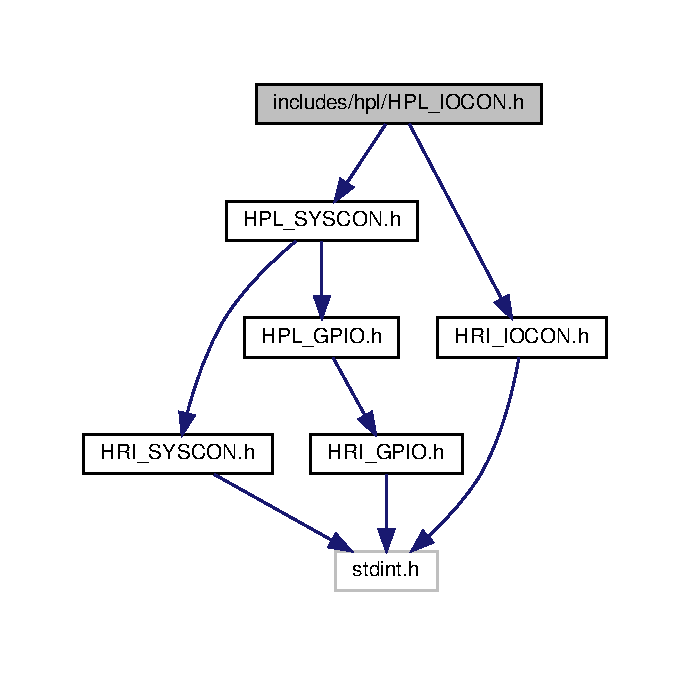
\includegraphics[width=331pt]{dc/d6c/HPL__IOCON_8h__incl}
\end{center}
\end{figure}
Gráfico de los archivos que directa o indirectamente incluyen a este archivo\+:\nopagebreak
\begin{figure}[H]
\begin{center}
\leavevmode
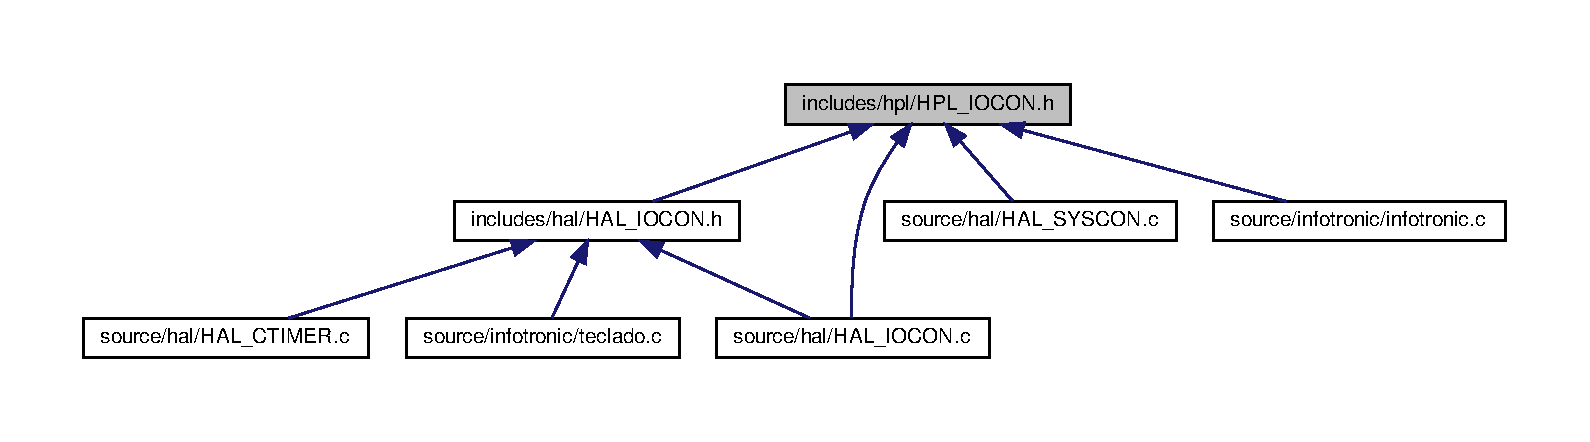
\includegraphics[width=350pt]{d5/d06/HPL__IOCON_8h__dep__incl}
\end{center}
\end{figure}
\subsection*{Enumeraciones}
\begin{DoxyCompactItemize}
\item 
\mbox{\Hypertarget{HPL__IOCON_8h_aa8ba7d9a2ec6e147ae5eeb52fa8fc1c7}\label{HPL__IOCON_8h_aa8ba7d9a2ec6e147ae5eeb52fa8fc1c7}} 
enum {\bfseries I\+O\+C\+O\+N\+\_\+pull\+\_\+mode\+\_\+en} \{ {\bfseries I\+O\+C\+O\+N\+\_\+\+P\+U\+L\+L\+\_\+\+N\+O\+NE} = 0, 
{\bfseries I\+O\+C\+O\+N\+\_\+\+P\+U\+L\+L\+\_\+\+D\+O\+WN}, 
{\bfseries I\+O\+C\+O\+N\+\_\+\+P\+U\+L\+L\+\_\+\+UP}, 
{\bfseries I\+O\+C\+O\+N\+\_\+\+P\+U\+L\+L\+\_\+\+R\+E\+P\+E\+A\+T\+ER}
 \}
\item 
\mbox{\Hypertarget{HPL__IOCON_8h_aeef5b33358336e2f33f7ab699d8d118f}\label{HPL__IOCON_8h_aeef5b33358336e2f33f7ab699d8d118f}} 
enum {\bfseries I\+O\+C\+O\+N\+\_\+sample\+\_\+mode\+\_\+en} \{ {\bfseries I\+O\+C\+O\+N\+\_\+\+S\+A\+M\+P\+L\+E\+\_\+\+M\+O\+D\+E\+\_\+\+B\+Y\+P\+A\+SS} = 0, 
{\bfseries I\+O\+C\+O\+N\+\_\+\+S\+A\+M\+P\+L\+E\+\_\+\+M\+O\+D\+E\+\_\+1\+\_\+\+C\+L\+O\+CK}, 
{\bfseries I\+O\+C\+O\+N\+\_\+\+S\+A\+M\+P\+L\+E\+\_\+\+M\+O\+D\+E\+\_\+2\+\_\+\+C\+L\+O\+CK}, 
{\bfseries I\+O\+C\+O\+N\+\_\+\+S\+A\+M\+P\+L\+E\+\_\+\+M\+O\+D\+E\+\_\+3\+\_\+\+C\+L\+O\+CK}
 \}
\item 
\mbox{\Hypertarget{HPL__IOCON_8h_a823cad956b251f0bff16c6992beb82a7}\label{HPL__IOCON_8h_a823cad956b251f0bff16c6992beb82a7}} 
enum {\bfseries I\+O\+C\+O\+N\+\_\+clk\+\_\+sel\+\_\+en} \{ \newline
{\bfseries I\+O\+C\+O\+N\+\_\+\+C\+L\+K\+\_\+\+D\+I\+V\+\_\+0} = 0, 
{\bfseries I\+O\+C\+O\+N\+\_\+\+C\+L\+K\+\_\+\+D\+I\+V\+\_\+1}, 
{\bfseries I\+O\+C\+O\+N\+\_\+\+C\+L\+K\+\_\+\+D\+I\+V\+\_\+2}, 
{\bfseries I\+O\+C\+O\+N\+\_\+\+C\+L\+K\+\_\+\+D\+I\+V\+\_\+3}, 
\newline
{\bfseries I\+O\+C\+O\+N\+\_\+\+C\+L\+K\+\_\+\+D\+I\+V\+\_\+4}, 
{\bfseries I\+O\+C\+O\+N\+\_\+\+C\+L\+K\+\_\+\+D\+I\+V\+\_\+5}, 
{\bfseries I\+O\+C\+O\+N\+\_\+\+C\+L\+K\+\_\+\+D\+I\+V\+\_\+6}
 \}
\item 
\mbox{\Hypertarget{HPL__IOCON_8h_a3434ae16a3ced0b0569ca1731bb008d1}\label{HPL__IOCON_8h_a3434ae16a3ced0b0569ca1731bb008d1}} 
enum {\bfseries I\+O\+C\+O\+N\+\_\+iic\+\_\+mode\+\_\+en} \{ {\bfseries I\+O\+C\+O\+N\+\_\+\+I\+I\+C\+\_\+\+M\+O\+D\+E\+\_\+\+S\+T\+A\+N\+D\+A\+RD} = 0, 
{\bfseries I\+O\+C\+O\+N\+\_\+\+I\+I\+C\+\_\+\+M\+O\+D\+E\+\_\+\+G\+P\+IO}, 
{\bfseries I\+O\+C\+O\+N\+\_\+\+I\+I\+C\+\_\+\+M\+O\+D\+E\+\_\+\+F\+A\+S\+T\+\_\+\+M\+O\+DE}
 \}
\end{DoxyCompactItemize}
\subsection*{Funciones}
\begin{DoxyCompactItemize}
\item 
static void \hyperlink{HPL__IOCON_8h_ac8a793d4b6c1f6eca58555f942ff721b}{I\+O\+C\+O\+N\+\_\+init} (void)
\begin{DoxyCompactList}\small\item\em Inicializacion del modulo I\+O\+C\+ON. \end{DoxyCompactList}\item 
static void \hyperlink{HPL__IOCON_8h_aa6a1f1da78d1e9eea04e2265daac7e1c}{I\+O\+C\+O\+N\+\_\+deinit} (void)
\begin{DoxyCompactList}\small\item\em Inhabilitacion del modulo I\+O\+C\+ON. \end{DoxyCompactList}\item 
static void \hyperlink{HPL__IOCON_8h_a531eb5245577caa96015eaceff8449a1}{I\+O\+C\+O\+N\+\_\+config\+\_\+pull\+\_\+mode} (uint8\+\_\+t port, uint8\+\_\+t pin, I\+O\+C\+O\+N\+\_\+pull\+\_\+mode\+\_\+en pull\+\_\+mode)
\begin{DoxyCompactList}\small\item\em Configurar modo de funcionamiento (pull up, pull down, etc) en un pin. \end{DoxyCompactList}\item 
static void \hyperlink{HPL__IOCON_8h_ac80b6a592161cd0f5124dbffafe552cb}{I\+O\+C\+O\+N\+\_\+enable\+\_\+hysteresis} (uint8\+\_\+t port, uint8\+\_\+t pin)
\begin{DoxyCompactList}\small\item\em Habilitar histeresis en un pin. \end{DoxyCompactList}\item 
static void \hyperlink{HPL__IOCON_8h_a657c0c0341ebbb9d43f4fbdf1a9027fb}{I\+O\+C\+O\+N\+\_\+disable\+\_\+hysteresis} (uint8\+\_\+t port, uint8\+\_\+t pin)
\begin{DoxyCompactList}\small\item\em Inhabilitar histeresis en un pin. \end{DoxyCompactList}\item 
static void \hyperlink{HPL__IOCON_8h_a2a9ae7bdc92fd6325ec38befb01feb51}{I\+O\+C\+O\+N\+\_\+enable\+\_\+invert} (uint8\+\_\+t port, uint8\+\_\+t pin)
\begin{DoxyCompactList}\small\item\em Habilitar inversion en un pin. \end{DoxyCompactList}\item 
static void \hyperlink{HPL__IOCON_8h_a434cae72963baffec893aa3b035c64fd}{I\+O\+C\+O\+N\+\_\+disable\+\_\+invert} (uint8\+\_\+t port, uint8\+\_\+t pin)
\begin{DoxyCompactList}\small\item\em Inhabilitar inversion en un pin. \end{DoxyCompactList}\item 
static void \hyperlink{HPL__IOCON_8h_aa774324a17698d6dc3054bed0e3322fe}{I\+O\+C\+O\+N\+\_\+enable\+\_\+open\+\_\+drain} (uint8\+\_\+t port, uint8\+\_\+t pin)
\begin{DoxyCompactList}\small\item\em Habilitar modo open drain en un pin. \end{DoxyCompactList}\item 
static void \hyperlink{HPL__IOCON_8h_abdece1a8e22fa543fcf02f54342c4f15}{I\+O\+C\+O\+N\+\_\+disable\+\_\+open\+\_\+drain} (uint8\+\_\+t port, uint8\+\_\+t pin)
\begin{DoxyCompactList}\small\item\em Inhabilitar modo open drain en un pin. \end{DoxyCompactList}\item 
static void \hyperlink{HPL__IOCON_8h_a25612d6c9182b6e8442548d48807239b}{I\+O\+C\+O\+N\+\_\+config\+\_\+sample\+\_\+mode} (uint8\+\_\+t port, uint8\+\_\+t pin, I\+O\+C\+O\+N\+\_\+sample\+\_\+mode\+\_\+en sample\+\_\+mode)
\begin{DoxyCompactList}\small\item\em Configurar modo de sampleo en un pin. \end{DoxyCompactList}\item 
static void \hyperlink{HPL__IOCON_8h_ac2081ddb1da6aaacf941a346387f896d}{I\+O\+C\+O\+N\+\_\+config\+\_\+clock\+\_\+source} (uint8\+\_\+t port, uint8\+\_\+t pin, I\+O\+C\+O\+N\+\_\+clk\+\_\+sel\+\_\+en clock\+\_\+source)
\begin{DoxyCompactList}\small\item\em Configurar fuente utilizada para el sampleo en un pin. \end{DoxyCompactList}\item 
\mbox{\Hypertarget{HPL__IOCON_8h_a23ad5a4fdce8f99274d24f6e6a7db41f}\label{HPL__IOCON_8h_a23ad5a4fdce8f99274d24f6e6a7db41f}} 
static void \hyperlink{HPL__IOCON_8h_a23ad5a4fdce8f99274d24f6e6a7db41f}{I\+O\+C\+O\+N\+\_\+enable\+\_\+dac0} (void)
\begin{DoxyCompactList}\small\item\em Habilitar D\+A\+C0 en P\+I\+O0\+\_\+17. \end{DoxyCompactList}\item 
\mbox{\Hypertarget{HPL__IOCON_8h_a9ee9d893a205ef3bc7a4f26c5abac66e}\label{HPL__IOCON_8h_a9ee9d893a205ef3bc7a4f26c5abac66e}} 
static void \hyperlink{HPL__IOCON_8h_a9ee9d893a205ef3bc7a4f26c5abac66e}{I\+O\+C\+O\+N\+\_\+enable\+\_\+dac1} (void)
\begin{DoxyCompactList}\small\item\em Habilitar D\+A\+C1 en P\+I\+O0\+\_\+29. \end{DoxyCompactList}\item 
\mbox{\Hypertarget{HPL__IOCON_8h_a5c8853d382380971b344feb2e9e0ac0d}\label{HPL__IOCON_8h_a5c8853d382380971b344feb2e9e0ac0d}} 
static void \hyperlink{HPL__IOCON_8h_a5c8853d382380971b344feb2e9e0ac0d}{I\+O\+C\+O\+N\+\_\+disable\+\_\+dac0} (void)
\begin{DoxyCompactList}\small\item\em Inhabilitar D\+A\+C0 en P\+I\+O0\+\_\+17. \end{DoxyCompactList}\item 
\mbox{\Hypertarget{HPL__IOCON_8h_affc3d0c98316505129248f5f421e675d}\label{HPL__IOCON_8h_affc3d0c98316505129248f5f421e675d}} 
static void \hyperlink{HPL__IOCON_8h_affc3d0c98316505129248f5f421e675d}{I\+O\+C\+O\+N\+\_\+disable\+\_\+dac1} (void)
\begin{DoxyCompactList}\small\item\em Inhabilitar D\+A\+C1 en P\+I\+O0\+\_\+29. \end{DoxyCompactList}\item 
static void \hyperlink{HPL__IOCON_8h_a866abbda2b6102011bb4a9341709ce8a}{I\+O\+C\+O\+N\+\_\+select\+\_\+iic0\+\_\+scl} (I\+O\+C\+O\+N\+\_\+iic\+\_\+mode\+\_\+en iic\+\_\+mode)
\begin{DoxyCompactList}\small\item\em Habilitar I\+I\+C0\+\_\+\+S\+CL en P\+I\+O0\+\_\+10. \end{DoxyCompactList}\item 
static void \hyperlink{HPL__IOCON_8h_a298d06693808eca45844c48c855a706c}{I\+O\+C\+O\+N\+\_\+select\+\_\+iic0\+\_\+sda} (I\+O\+C\+O\+N\+\_\+iic\+\_\+mode\+\_\+en iic\+\_\+mode)
\begin{DoxyCompactList}\small\item\em Habilitar I\+IC S\+DA en P\+I\+O0\+\_\+11. \end{DoxyCompactList}\end{DoxyCompactItemize}
\subsection*{Variables}
\begin{DoxyCompactItemize}
\item 
\mbox{\Hypertarget{HPL__IOCON_8h_a446b5ff38614b88495bb5a5d7574f96d}\label{HPL__IOCON_8h_a446b5ff38614b88495bb5a5d7574f96d}} 
volatile \hyperlink{structIOCON__per__t}{I\+O\+C\+O\+N\+\_\+per\+\_\+t} $\ast$const \hyperlink{HPL__IOCON_8h_a446b5ff38614b88495bb5a5d7574f96d}{I\+O\+C\+ON}
\begin{DoxyCompactList}\small\item\em Periferico I\+O\+C\+ON. \end{DoxyCompactList}\item 
\mbox{\Hypertarget{HPL__IOCON_8h_a3eabc50cf92c5f45256fa84022787c2b}\label{HPL__IOCON_8h_a3eabc50cf92c5f45256fa84022787c2b}} 
volatile \hyperlink{structIOCON__PIO__reg__t}{I\+O\+C\+O\+N\+\_\+\+P\+I\+O\+\_\+reg\+\_\+t} $\ast$const \hyperlink{HPL__IOCON_8h_a3eabc50cf92c5f45256fa84022787c2b}{I\+O\+C\+O\+N\+\_\+\+P\+I\+N\+\_\+\+T\+A\+B\+LE} \mbox{[}2\mbox{]}\mbox{[}32\mbox{]}
\begin{DoxyCompactList}\small\item\em Tabla de registros de configuracion. \end{DoxyCompactList}\end{DoxyCompactItemize}


\subsection{Descripción detallada}
Declaraciones a nivel de abstraccion de periferico del I\+O\+C\+ON (L\+P\+C845) 

\begin{DoxyAuthor}{Autor}
Augusto Santini 
\end{DoxyAuthor}
\begin{DoxyDate}{Fecha}
6/2019 
\end{DoxyDate}
\begin{DoxyVersion}{Versión}
1.\+0 
\end{DoxyVersion}


\subsection{Documentación de las funciones}
\mbox{\Hypertarget{HPL__IOCON_8h_ac8a793d4b6c1f6eca58555f942ff721b}\label{HPL__IOCON_8h_ac8a793d4b6c1f6eca58555f942ff721b}} 
\index{H\+P\+L\+\_\+\+I\+O\+C\+O\+N.\+h@{H\+P\+L\+\_\+\+I\+O\+C\+O\+N.\+h}!I\+O\+C\+O\+N\+\_\+init@{I\+O\+C\+O\+N\+\_\+init}}
\index{I\+O\+C\+O\+N\+\_\+init@{I\+O\+C\+O\+N\+\_\+init}!H\+P\+L\+\_\+\+I\+O\+C\+O\+N.\+h@{H\+P\+L\+\_\+\+I\+O\+C\+O\+N.\+h}}
\subsubsection{\texorpdfstring{I\+O\+C\+O\+N\+\_\+init()}{IOCON\_init()}}
{\footnotesize\ttfamily static void I\+O\+C\+O\+N\+\_\+init (\begin{DoxyParamCaption}\item[{void}]{ }\end{DoxyParamCaption})\hspace{0.3cm}{\ttfamily [inline]}, {\ttfamily [static]}}



Inicializacion del modulo I\+O\+C\+ON. 

Unicamente habilita el clock del modulo \mbox{\Hypertarget{HPL__IOCON_8h_aa6a1f1da78d1e9eea04e2265daac7e1c}\label{HPL__IOCON_8h_aa6a1f1da78d1e9eea04e2265daac7e1c}} 
\index{H\+P\+L\+\_\+\+I\+O\+C\+O\+N.\+h@{H\+P\+L\+\_\+\+I\+O\+C\+O\+N.\+h}!I\+O\+C\+O\+N\+\_\+deinit@{I\+O\+C\+O\+N\+\_\+deinit}}
\index{I\+O\+C\+O\+N\+\_\+deinit@{I\+O\+C\+O\+N\+\_\+deinit}!H\+P\+L\+\_\+\+I\+O\+C\+O\+N.\+h@{H\+P\+L\+\_\+\+I\+O\+C\+O\+N.\+h}}
\subsubsection{\texorpdfstring{I\+O\+C\+O\+N\+\_\+deinit()}{IOCON\_deinit()}}
{\footnotesize\ttfamily static void I\+O\+C\+O\+N\+\_\+deinit (\begin{DoxyParamCaption}\item[{void}]{ }\end{DoxyParamCaption})\hspace{0.3cm}{\ttfamily [inline]}, {\ttfamily [static]}}



Inhabilitacion del modulo I\+O\+C\+ON. 

Unicamente inhabilita el clock del modulo \mbox{\Hypertarget{HPL__IOCON_8h_a531eb5245577caa96015eaceff8449a1}\label{HPL__IOCON_8h_a531eb5245577caa96015eaceff8449a1}} 
\index{H\+P\+L\+\_\+\+I\+O\+C\+O\+N.\+h@{H\+P\+L\+\_\+\+I\+O\+C\+O\+N.\+h}!I\+O\+C\+O\+N\+\_\+config\+\_\+pull\+\_\+mode@{I\+O\+C\+O\+N\+\_\+config\+\_\+pull\+\_\+mode}}
\index{I\+O\+C\+O\+N\+\_\+config\+\_\+pull\+\_\+mode@{I\+O\+C\+O\+N\+\_\+config\+\_\+pull\+\_\+mode}!H\+P\+L\+\_\+\+I\+O\+C\+O\+N.\+h@{H\+P\+L\+\_\+\+I\+O\+C\+O\+N.\+h}}
\subsubsection{\texorpdfstring{I\+O\+C\+O\+N\+\_\+config\+\_\+pull\+\_\+mode()}{IOCON\_config\_pull\_mode()}}
{\footnotesize\ttfamily static void I\+O\+C\+O\+N\+\_\+config\+\_\+pull\+\_\+mode (\begin{DoxyParamCaption}\item[{uint8\+\_\+t}]{port,  }\item[{uint8\+\_\+t}]{pin,  }\item[{I\+O\+C\+O\+N\+\_\+pull\+\_\+mode\+\_\+en}]{pull\+\_\+mode }\end{DoxyParamCaption})\hspace{0.3cm}{\ttfamily [inline]}, {\ttfamily [static]}}



Configurar modo de funcionamiento (pull up, pull down, etc) en un pin. 


\begin{DoxyParams}[1]{Parámetros}
\mbox{\tt in}  & {\em port} & Numero de puerto \\
\hline
\mbox{\tt in}  & {\em pin} & Numero de pin \\
\hline
\mbox{\tt in}  & {\em pull\+\_\+mode} & Modo de funcionamiento \\
\hline
\end{DoxyParams}
\mbox{\Hypertarget{HPL__IOCON_8h_ac80b6a592161cd0f5124dbffafe552cb}\label{HPL__IOCON_8h_ac80b6a592161cd0f5124dbffafe552cb}} 
\index{H\+P\+L\+\_\+\+I\+O\+C\+O\+N.\+h@{H\+P\+L\+\_\+\+I\+O\+C\+O\+N.\+h}!I\+O\+C\+O\+N\+\_\+enable\+\_\+hysteresis@{I\+O\+C\+O\+N\+\_\+enable\+\_\+hysteresis}}
\index{I\+O\+C\+O\+N\+\_\+enable\+\_\+hysteresis@{I\+O\+C\+O\+N\+\_\+enable\+\_\+hysteresis}!H\+P\+L\+\_\+\+I\+O\+C\+O\+N.\+h@{H\+P\+L\+\_\+\+I\+O\+C\+O\+N.\+h}}
\subsubsection{\texorpdfstring{I\+O\+C\+O\+N\+\_\+enable\+\_\+hysteresis()}{IOCON\_enable\_hysteresis()}}
{\footnotesize\ttfamily static void I\+O\+C\+O\+N\+\_\+enable\+\_\+hysteresis (\begin{DoxyParamCaption}\item[{uint8\+\_\+t}]{port,  }\item[{uint8\+\_\+t}]{pin }\end{DoxyParamCaption})\hspace{0.3cm}{\ttfamily [inline]}, {\ttfamily [static]}}



Habilitar histeresis en un pin. 


\begin{DoxyParams}[1]{Parámetros}
\mbox{\tt in}  & {\em port} & Numero de puerto \\
\hline
\mbox{\tt in}  & {\em pin} & Numero de pin \\
\hline
\end{DoxyParams}
\mbox{\Hypertarget{HPL__IOCON_8h_a657c0c0341ebbb9d43f4fbdf1a9027fb}\label{HPL__IOCON_8h_a657c0c0341ebbb9d43f4fbdf1a9027fb}} 
\index{H\+P\+L\+\_\+\+I\+O\+C\+O\+N.\+h@{H\+P\+L\+\_\+\+I\+O\+C\+O\+N.\+h}!I\+O\+C\+O\+N\+\_\+disable\+\_\+hysteresis@{I\+O\+C\+O\+N\+\_\+disable\+\_\+hysteresis}}
\index{I\+O\+C\+O\+N\+\_\+disable\+\_\+hysteresis@{I\+O\+C\+O\+N\+\_\+disable\+\_\+hysteresis}!H\+P\+L\+\_\+\+I\+O\+C\+O\+N.\+h@{H\+P\+L\+\_\+\+I\+O\+C\+O\+N.\+h}}
\subsubsection{\texorpdfstring{I\+O\+C\+O\+N\+\_\+disable\+\_\+hysteresis()}{IOCON\_disable\_hysteresis()}}
{\footnotesize\ttfamily static void I\+O\+C\+O\+N\+\_\+disable\+\_\+hysteresis (\begin{DoxyParamCaption}\item[{uint8\+\_\+t}]{port,  }\item[{uint8\+\_\+t}]{pin }\end{DoxyParamCaption})\hspace{0.3cm}{\ttfamily [inline]}, {\ttfamily [static]}}



Inhabilitar histeresis en un pin. 


\begin{DoxyParams}[1]{Parámetros}
\mbox{\tt in}  & {\em port} & Numero de puerto \\
\hline
\mbox{\tt in}  & {\em pin} & Numero de pin \\
\hline
\end{DoxyParams}
\mbox{\Hypertarget{HPL__IOCON_8h_a2a9ae7bdc92fd6325ec38befb01feb51}\label{HPL__IOCON_8h_a2a9ae7bdc92fd6325ec38befb01feb51}} 
\index{H\+P\+L\+\_\+\+I\+O\+C\+O\+N.\+h@{H\+P\+L\+\_\+\+I\+O\+C\+O\+N.\+h}!I\+O\+C\+O\+N\+\_\+enable\+\_\+invert@{I\+O\+C\+O\+N\+\_\+enable\+\_\+invert}}
\index{I\+O\+C\+O\+N\+\_\+enable\+\_\+invert@{I\+O\+C\+O\+N\+\_\+enable\+\_\+invert}!H\+P\+L\+\_\+\+I\+O\+C\+O\+N.\+h@{H\+P\+L\+\_\+\+I\+O\+C\+O\+N.\+h}}
\subsubsection{\texorpdfstring{I\+O\+C\+O\+N\+\_\+enable\+\_\+invert()}{IOCON\_enable\_invert()}}
{\footnotesize\ttfamily static void I\+O\+C\+O\+N\+\_\+enable\+\_\+invert (\begin{DoxyParamCaption}\item[{uint8\+\_\+t}]{port,  }\item[{uint8\+\_\+t}]{pin }\end{DoxyParamCaption})\hspace{0.3cm}{\ttfamily [inline]}, {\ttfamily [static]}}



Habilitar inversion en un pin. 


\begin{DoxyParams}[1]{Parámetros}
\mbox{\tt in}  & {\em port} & Numero de puerto \\
\hline
\mbox{\tt in}  & {\em pin} & Numero de pin \\
\hline
\end{DoxyParams}
\mbox{\Hypertarget{HPL__IOCON_8h_a434cae72963baffec893aa3b035c64fd}\label{HPL__IOCON_8h_a434cae72963baffec893aa3b035c64fd}} 
\index{H\+P\+L\+\_\+\+I\+O\+C\+O\+N.\+h@{H\+P\+L\+\_\+\+I\+O\+C\+O\+N.\+h}!I\+O\+C\+O\+N\+\_\+disable\+\_\+invert@{I\+O\+C\+O\+N\+\_\+disable\+\_\+invert}}
\index{I\+O\+C\+O\+N\+\_\+disable\+\_\+invert@{I\+O\+C\+O\+N\+\_\+disable\+\_\+invert}!H\+P\+L\+\_\+\+I\+O\+C\+O\+N.\+h@{H\+P\+L\+\_\+\+I\+O\+C\+O\+N.\+h}}
\subsubsection{\texorpdfstring{I\+O\+C\+O\+N\+\_\+disable\+\_\+invert()}{IOCON\_disable\_invert()}}
{\footnotesize\ttfamily static void I\+O\+C\+O\+N\+\_\+disable\+\_\+invert (\begin{DoxyParamCaption}\item[{uint8\+\_\+t}]{port,  }\item[{uint8\+\_\+t}]{pin }\end{DoxyParamCaption})\hspace{0.3cm}{\ttfamily [inline]}, {\ttfamily [static]}}



Inhabilitar inversion en un pin. 


\begin{DoxyParams}[1]{Parámetros}
\mbox{\tt in}  & {\em port} & Numero de puerto \\
\hline
\mbox{\tt in}  & {\em pin} & Numero de pin \\
\hline
\end{DoxyParams}
\mbox{\Hypertarget{HPL__IOCON_8h_aa774324a17698d6dc3054bed0e3322fe}\label{HPL__IOCON_8h_aa774324a17698d6dc3054bed0e3322fe}} 
\index{H\+P\+L\+\_\+\+I\+O\+C\+O\+N.\+h@{H\+P\+L\+\_\+\+I\+O\+C\+O\+N.\+h}!I\+O\+C\+O\+N\+\_\+enable\+\_\+open\+\_\+drain@{I\+O\+C\+O\+N\+\_\+enable\+\_\+open\+\_\+drain}}
\index{I\+O\+C\+O\+N\+\_\+enable\+\_\+open\+\_\+drain@{I\+O\+C\+O\+N\+\_\+enable\+\_\+open\+\_\+drain}!H\+P\+L\+\_\+\+I\+O\+C\+O\+N.\+h@{H\+P\+L\+\_\+\+I\+O\+C\+O\+N.\+h}}
\subsubsection{\texorpdfstring{I\+O\+C\+O\+N\+\_\+enable\+\_\+open\+\_\+drain()}{IOCON\_enable\_open\_drain()}}
{\footnotesize\ttfamily static void I\+O\+C\+O\+N\+\_\+enable\+\_\+open\+\_\+drain (\begin{DoxyParamCaption}\item[{uint8\+\_\+t}]{port,  }\item[{uint8\+\_\+t}]{pin }\end{DoxyParamCaption})\hspace{0.3cm}{\ttfamily [inline]}, {\ttfamily [static]}}



Habilitar modo open drain en un pin. 


\begin{DoxyParams}[1]{Parámetros}
\mbox{\tt in}  & {\em port} & Numero de puerto \\
\hline
\mbox{\tt in}  & {\em pin} & Numero de pin \\
\hline
\end{DoxyParams}
\mbox{\Hypertarget{HPL__IOCON_8h_abdece1a8e22fa543fcf02f54342c4f15}\label{HPL__IOCON_8h_abdece1a8e22fa543fcf02f54342c4f15}} 
\index{H\+P\+L\+\_\+\+I\+O\+C\+O\+N.\+h@{H\+P\+L\+\_\+\+I\+O\+C\+O\+N.\+h}!I\+O\+C\+O\+N\+\_\+disable\+\_\+open\+\_\+drain@{I\+O\+C\+O\+N\+\_\+disable\+\_\+open\+\_\+drain}}
\index{I\+O\+C\+O\+N\+\_\+disable\+\_\+open\+\_\+drain@{I\+O\+C\+O\+N\+\_\+disable\+\_\+open\+\_\+drain}!H\+P\+L\+\_\+\+I\+O\+C\+O\+N.\+h@{H\+P\+L\+\_\+\+I\+O\+C\+O\+N.\+h}}
\subsubsection{\texorpdfstring{I\+O\+C\+O\+N\+\_\+disable\+\_\+open\+\_\+drain()}{IOCON\_disable\_open\_drain()}}
{\footnotesize\ttfamily static void I\+O\+C\+O\+N\+\_\+disable\+\_\+open\+\_\+drain (\begin{DoxyParamCaption}\item[{uint8\+\_\+t}]{port,  }\item[{uint8\+\_\+t}]{pin }\end{DoxyParamCaption})\hspace{0.3cm}{\ttfamily [inline]}, {\ttfamily [static]}}



Inhabilitar modo open drain en un pin. 


\begin{DoxyParams}[1]{Parámetros}
\mbox{\tt in}  & {\em port} & Numero de puerto \\
\hline
\mbox{\tt in}  & {\em pin} & Numero de pin \\
\hline
\end{DoxyParams}
\mbox{\Hypertarget{HPL__IOCON_8h_a25612d6c9182b6e8442548d48807239b}\label{HPL__IOCON_8h_a25612d6c9182b6e8442548d48807239b}} 
\index{H\+P\+L\+\_\+\+I\+O\+C\+O\+N.\+h@{H\+P\+L\+\_\+\+I\+O\+C\+O\+N.\+h}!I\+O\+C\+O\+N\+\_\+config\+\_\+sample\+\_\+mode@{I\+O\+C\+O\+N\+\_\+config\+\_\+sample\+\_\+mode}}
\index{I\+O\+C\+O\+N\+\_\+config\+\_\+sample\+\_\+mode@{I\+O\+C\+O\+N\+\_\+config\+\_\+sample\+\_\+mode}!H\+P\+L\+\_\+\+I\+O\+C\+O\+N.\+h@{H\+P\+L\+\_\+\+I\+O\+C\+O\+N.\+h}}
\subsubsection{\texorpdfstring{I\+O\+C\+O\+N\+\_\+config\+\_\+sample\+\_\+mode()}{IOCON\_config\_sample\_mode()}}
{\footnotesize\ttfamily static void I\+O\+C\+O\+N\+\_\+config\+\_\+sample\+\_\+mode (\begin{DoxyParamCaption}\item[{uint8\+\_\+t}]{port,  }\item[{uint8\+\_\+t}]{pin,  }\item[{I\+O\+C\+O\+N\+\_\+sample\+\_\+mode\+\_\+en}]{sample\+\_\+mode }\end{DoxyParamCaption})\hspace{0.3cm}{\ttfamily [inline]}, {\ttfamily [static]}}



Configurar modo de sampleo en un pin. 


\begin{DoxyParams}[1]{Parámetros}
\mbox{\tt in}  & {\em port} & Numero de puerto \\
\hline
\mbox{\tt in}  & {\em pin} & Numero de pin \\
\hline
\mbox{\tt in}  & {\em sample\+\_\+mode} & Modo de sampleo \\
\hline
\end{DoxyParams}
\mbox{\Hypertarget{HPL__IOCON_8h_ac2081ddb1da6aaacf941a346387f896d}\label{HPL__IOCON_8h_ac2081ddb1da6aaacf941a346387f896d}} 
\index{H\+P\+L\+\_\+\+I\+O\+C\+O\+N.\+h@{H\+P\+L\+\_\+\+I\+O\+C\+O\+N.\+h}!I\+O\+C\+O\+N\+\_\+config\+\_\+clock\+\_\+source@{I\+O\+C\+O\+N\+\_\+config\+\_\+clock\+\_\+source}}
\index{I\+O\+C\+O\+N\+\_\+config\+\_\+clock\+\_\+source@{I\+O\+C\+O\+N\+\_\+config\+\_\+clock\+\_\+source}!H\+P\+L\+\_\+\+I\+O\+C\+O\+N.\+h@{H\+P\+L\+\_\+\+I\+O\+C\+O\+N.\+h}}
\subsubsection{\texorpdfstring{I\+O\+C\+O\+N\+\_\+config\+\_\+clock\+\_\+source()}{IOCON\_config\_clock\_source()}}
{\footnotesize\ttfamily static void I\+O\+C\+O\+N\+\_\+config\+\_\+clock\+\_\+source (\begin{DoxyParamCaption}\item[{uint8\+\_\+t}]{port,  }\item[{uint8\+\_\+t}]{pin,  }\item[{I\+O\+C\+O\+N\+\_\+clk\+\_\+sel\+\_\+en}]{clock\+\_\+source }\end{DoxyParamCaption})\hspace{0.3cm}{\ttfamily [inline]}, {\ttfamily [static]}}



Configurar fuente utilizada para el sampleo en un pin. 


\begin{DoxyParams}[1]{Parámetros}
\mbox{\tt in}  & {\em port} & Numero de puerto \\
\hline
\mbox{\tt in}  & {\em pin} & Numero de pin \\
\hline
\mbox{\tt in}  & {\em clock\+\_\+source} & Fuente de clock deseada \\
\hline
\end{DoxyParams}
\mbox{\Hypertarget{HPL__IOCON_8h_a866abbda2b6102011bb4a9341709ce8a}\label{HPL__IOCON_8h_a866abbda2b6102011bb4a9341709ce8a}} 
\index{H\+P\+L\+\_\+\+I\+O\+C\+O\+N.\+h@{H\+P\+L\+\_\+\+I\+O\+C\+O\+N.\+h}!I\+O\+C\+O\+N\+\_\+select\+\_\+iic0\+\_\+scl@{I\+O\+C\+O\+N\+\_\+select\+\_\+iic0\+\_\+scl}}
\index{I\+O\+C\+O\+N\+\_\+select\+\_\+iic0\+\_\+scl@{I\+O\+C\+O\+N\+\_\+select\+\_\+iic0\+\_\+scl}!H\+P\+L\+\_\+\+I\+O\+C\+O\+N.\+h@{H\+P\+L\+\_\+\+I\+O\+C\+O\+N.\+h}}
\subsubsection{\texorpdfstring{I\+O\+C\+O\+N\+\_\+select\+\_\+iic0\+\_\+scl()}{IOCON\_select\_iic0\_scl()}}
{\footnotesize\ttfamily static void I\+O\+C\+O\+N\+\_\+select\+\_\+iic0\+\_\+scl (\begin{DoxyParamCaption}\item[{I\+O\+C\+O\+N\+\_\+iic\+\_\+mode\+\_\+en}]{iic\+\_\+mode }\end{DoxyParamCaption})\hspace{0.3cm}{\ttfamily [inline]}, {\ttfamily [static]}}



Habilitar I\+I\+C0\+\_\+\+S\+CL en P\+I\+O0\+\_\+10. 


\begin{DoxyParams}[1]{Parámetros}
\mbox{\tt in}  & {\em iic\+\_\+mode} & Modo de I\+IC \\
\hline
\end{DoxyParams}
\mbox{\Hypertarget{HPL__IOCON_8h_a298d06693808eca45844c48c855a706c}\label{HPL__IOCON_8h_a298d06693808eca45844c48c855a706c}} 
\index{H\+P\+L\+\_\+\+I\+O\+C\+O\+N.\+h@{H\+P\+L\+\_\+\+I\+O\+C\+O\+N.\+h}!I\+O\+C\+O\+N\+\_\+select\+\_\+iic0\+\_\+sda@{I\+O\+C\+O\+N\+\_\+select\+\_\+iic0\+\_\+sda}}
\index{I\+O\+C\+O\+N\+\_\+select\+\_\+iic0\+\_\+sda@{I\+O\+C\+O\+N\+\_\+select\+\_\+iic0\+\_\+sda}!H\+P\+L\+\_\+\+I\+O\+C\+O\+N.\+h@{H\+P\+L\+\_\+\+I\+O\+C\+O\+N.\+h}}
\subsubsection{\texorpdfstring{I\+O\+C\+O\+N\+\_\+select\+\_\+iic0\+\_\+sda()}{IOCON\_select\_iic0\_sda()}}
{\footnotesize\ttfamily static void I\+O\+C\+O\+N\+\_\+select\+\_\+iic0\+\_\+sda (\begin{DoxyParamCaption}\item[{I\+O\+C\+O\+N\+\_\+iic\+\_\+mode\+\_\+en}]{iic\+\_\+mode }\end{DoxyParamCaption})\hspace{0.3cm}{\ttfamily [inline]}, {\ttfamily [static]}}



Habilitar I\+IC S\+DA en P\+I\+O0\+\_\+11. 


\begin{DoxyParams}[1]{Parámetros}
\mbox{\tt in}  & {\em iic\+\_\+mode} & Modo de I\+IC \\
\hline
\end{DoxyParams}

\hypertarget{HPL__MRT_8h}{}\section{Referencia del Archivo includes/hpl/\+H\+P\+L\+\_\+\+M\+RT.h}
\label{HPL__MRT_8h}\index{includes/hpl/\+H\+P\+L\+\_\+\+M\+R\+T.\+h@{includes/hpl/\+H\+P\+L\+\_\+\+M\+R\+T.\+h}}


Declaraciones a nivel de abstraccion de periferico del M\+RT (L\+P\+C845)  


{\ttfamily \#include $<$H\+R\+I\+\_\+\+M\+R\+T.\+h$>$}\newline
Dependencia gráfica adjunta para H\+P\+L\+\_\+\+M\+R\+T.\+h\+:
\nopagebreak
\begin{figure}[H]
\begin{center}
\leavevmode
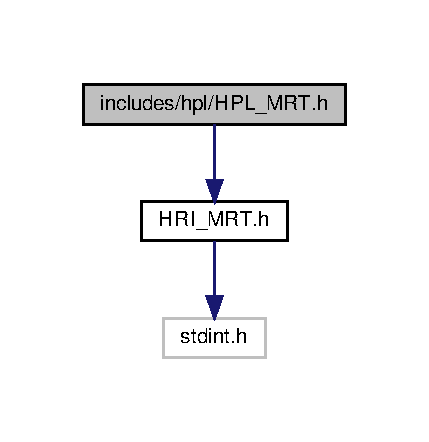
\includegraphics[width=206pt]{db/d0b/HPL__MRT_8h__incl}
\end{center}
\end{figure}
\subsection*{Enumeraciones}
\begin{DoxyCompactItemize}
\item 
\mbox{\Hypertarget{HPL__MRT_8h_a1833cab768b3dc0a6b3cc1cc90df559e}\label{HPL__MRT_8h_a1833cab768b3dc0a6b3cc1cc90df559e}} 
enum {\bfseries M\+R\+T\+\_\+channel\+\_\+sel\+\_\+en} \{ {\bfseries M\+R\+T\+\_\+\+C\+H\+A\+N\+N\+E\+L\+\_\+0} = 0, 
{\bfseries M\+R\+T\+\_\+\+C\+H\+A\+N\+N\+E\+L\+\_\+1}, 
{\bfseries M\+R\+T\+\_\+\+C\+H\+A\+N\+N\+E\+L\+\_\+2}, 
{\bfseries M\+R\+T\+\_\+\+C\+H\+A\+N\+N\+E\+L\+\_\+3}
 \}
\item 
\mbox{\Hypertarget{HPL__MRT_8h_ad20a3a0ffe751bd956a15412cc13fd8a}\label{HPL__MRT_8h_ad20a3a0ffe751bd956a15412cc13fd8a}} 
enum {\bfseries M\+R\+T\+\_\+mode\+\_\+en} \{ {\bfseries M\+R\+T\+\_\+\+M\+O\+D\+E\+\_\+\+R\+E\+P\+E\+AT} = 0, 
{\bfseries M\+R\+T\+\_\+\+M\+O\+D\+E\+\_\+\+O\+N\+E\+\_\+\+S\+H\+OT}, 
{\bfseries M\+R\+T\+\_\+\+M\+O\+D\+E\+\_\+\+O\+N\+E\+\_\+\+S\+H\+O\+T\+\_\+\+B\+U\+S\+\_\+\+S\+T\+A\+LL}
 \}
\end{DoxyCompactItemize}
\subsection*{Funciones}
\begin{DoxyCompactItemize}
\item 
static void \hyperlink{HPL__MRT_8h_a63c0887416689930fa0b2440a0d36afa}{M\+R\+T\+\_\+set\+\_\+interval} (M\+R\+T\+\_\+channel\+\_\+sel\+\_\+en channel, uint32\+\_\+t interval)
\begin{DoxyCompactList}\small\item\em Fijar intervalo de un canal del M\+RT sin detener el conteo actual. \end{DoxyCompactList}\item 
static void \hyperlink{HPL__MRT_8h_a1368fc13d7cd7f4167738281380d56ac}{M\+R\+T\+\_\+set\+\_\+interval\+\_\+and\+\_\+stop\+\_\+timer} (M\+R\+T\+\_\+channel\+\_\+sel\+\_\+en channel, uint32\+\_\+t interval)
\begin{DoxyCompactList}\small\item\em Fijar intervalo de un canal del M\+RT deteniendo el conteo actual inmediatamente. \end{DoxyCompactList}\item 
static uint32\+\_\+t \hyperlink{HPL__MRT_8h_a08b75e369a8bc8a498ec27b8903ffa89}{M\+R\+T\+\_\+get\+\_\+current\+\_\+value} (M\+R\+T\+\_\+channel\+\_\+sel\+\_\+en channel)
\begin{DoxyCompactList}\small\item\em Obtener el valor de la cuenta actual de un canal del M\+RT. \end{DoxyCompactList}\item 
\mbox{\Hypertarget{HPL__MRT_8h_a494c25fbef4c05cd994f5d9c184f50c0}\label{HPL__MRT_8h_a494c25fbef4c05cd994f5d9c184f50c0}} 
static void {\bfseries M\+R\+T\+\_\+enable\+\_\+irq} (M\+R\+T\+\_\+channel\+\_\+sel\+\_\+en channel)
\item 
\mbox{\Hypertarget{HPL__MRT_8h_ae6932dc74f2e4ddabfaeac00bdf2d41a}\label{HPL__MRT_8h_ae6932dc74f2e4ddabfaeac00bdf2d41a}} 
static void {\bfseries M\+R\+T\+\_\+disable\+\_\+irq} (M\+R\+T\+\_\+channel\+\_\+sel\+\_\+en channel)
\item 
static void \hyperlink{HPL__MRT_8h_a41688adbcd5743919a123f2c6de108cd}{M\+R\+T\+\_\+config\+\_\+mode} (M\+R\+T\+\_\+channel\+\_\+sel\+\_\+en channel, M\+R\+T\+\_\+mode\+\_\+en mode)
\begin{DoxyCompactList}\small\item\em Configurar modo de funcionamiento de un canal del M\+RT. \end{DoxyCompactList}\item 
static uint8\+\_\+t \hyperlink{HPL__MRT_8h_ade5ba4007e452503ef2c39c22b28613b}{M\+R\+T\+\_\+get\+\_\+idle\+\_\+channel} (void)
\begin{DoxyCompactList}\small\item\em Obtener el canal que este en estado I\+D\+LE. \end{DoxyCompactList}\item 
static uint8\+\_\+t \hyperlink{HPL__MRT_8h_afcbf27c3ca99f0b0f8094ba6dea4d5d9}{M\+R\+T\+\_\+get\+\_\+irq\+\_\+flag} (M\+R\+T\+\_\+channel\+\_\+sel\+\_\+en channel)
\begin{DoxyCompactList}\small\item\em Obtener flag de interrupcion de un canal. \end{DoxyCompactList}\item 
static void \hyperlink{HPL__MRT_8h_a0c850363425d78f9d5d7521ab70d0c4f}{M\+R\+T\+\_\+clear\+\_\+irq\+\_\+flag} (M\+R\+T\+\_\+channel\+\_\+sel\+\_\+en channel)
\begin{DoxyCompactList}\small\item\em Limpiar flag de interrupcion de un canal. \end{DoxyCompactList}\end{DoxyCompactItemize}
\subsection*{Variables}
\begin{DoxyCompactItemize}
\item 
\mbox{\Hypertarget{HPL__MRT_8h_aa02bb3fa0854b46bd753e434ef216e83}\label{HPL__MRT_8h_aa02bb3fa0854b46bd753e434ef216e83}} 
volatile \hyperlink{HRI__MRT_8h_de/dfc/structMRT__per__t}{M\+R\+T\+\_\+per\+\_\+t} $\ast$const \hyperlink{HPL__MRT_8h_aa02bb3fa0854b46bd753e434ef216e83}{M\+RT}
\begin{DoxyCompactList}\small\item\em Periferico M\+RT. \end{DoxyCompactList}\end{DoxyCompactItemize}


\subsection{Descripción detallada}
Declaraciones a nivel de abstraccion de periferico del M\+RT (L\+P\+C845) 

\begin{DoxyAuthor}{Autor}
Augusto Santini 
\end{DoxyAuthor}
\begin{DoxyDate}{Fecha}
4/2020 
\end{DoxyDate}
\begin{DoxyVersion}{Versión}
1.\+0 
\end{DoxyVersion}


\subsection{Documentación de las funciones}
\mbox{\Hypertarget{HPL__MRT_8h_a63c0887416689930fa0b2440a0d36afa}\label{HPL__MRT_8h_a63c0887416689930fa0b2440a0d36afa}} 
\index{H\+P\+L\+\_\+\+M\+R\+T.\+h@{H\+P\+L\+\_\+\+M\+R\+T.\+h}!M\+R\+T\+\_\+set\+\_\+interval@{M\+R\+T\+\_\+set\+\_\+interval}}
\index{M\+R\+T\+\_\+set\+\_\+interval@{M\+R\+T\+\_\+set\+\_\+interval}!H\+P\+L\+\_\+\+M\+R\+T.\+h@{H\+P\+L\+\_\+\+M\+R\+T.\+h}}
\subsubsection{\texorpdfstring{M\+R\+T\+\_\+set\+\_\+interval()}{MRT\_set\_interval()}}
{\footnotesize\ttfamily static void M\+R\+T\+\_\+set\+\_\+interval (\begin{DoxyParamCaption}\item[{M\+R\+T\+\_\+channel\+\_\+sel\+\_\+en}]{channel,  }\item[{uint32\+\_\+t}]{interval }\end{DoxyParamCaption})\hspace{0.3cm}{\ttfamily [inline]}, {\ttfamily [static]}}



Fijar intervalo de un canal del M\+RT sin detener el conteo actual. 


\begin{DoxyParams}[1]{Parámetros}
\mbox{\tt in}  & {\em channel} & Canal a configurar \\
\hline
\mbox{\tt in}  & {\em interval} & Intervalo a cargar \\
\hline
\end{DoxyParams}
\mbox{\Hypertarget{HPL__MRT_8h_a1368fc13d7cd7f4167738281380d56ac}\label{HPL__MRT_8h_a1368fc13d7cd7f4167738281380d56ac}} 
\index{H\+P\+L\+\_\+\+M\+R\+T.\+h@{H\+P\+L\+\_\+\+M\+R\+T.\+h}!M\+R\+T\+\_\+set\+\_\+interval\+\_\+and\+\_\+stop\+\_\+timer@{M\+R\+T\+\_\+set\+\_\+interval\+\_\+and\+\_\+stop\+\_\+timer}}
\index{M\+R\+T\+\_\+set\+\_\+interval\+\_\+and\+\_\+stop\+\_\+timer@{M\+R\+T\+\_\+set\+\_\+interval\+\_\+and\+\_\+stop\+\_\+timer}!H\+P\+L\+\_\+\+M\+R\+T.\+h@{H\+P\+L\+\_\+\+M\+R\+T.\+h}}
\subsubsection{\texorpdfstring{M\+R\+T\+\_\+set\+\_\+interval\+\_\+and\+\_\+stop\+\_\+timer()}{MRT\_set\_interval\_and\_stop\_timer()}}
{\footnotesize\ttfamily static void M\+R\+T\+\_\+set\+\_\+interval\+\_\+and\+\_\+stop\+\_\+timer (\begin{DoxyParamCaption}\item[{M\+R\+T\+\_\+channel\+\_\+sel\+\_\+en}]{channel,  }\item[{uint32\+\_\+t}]{interval }\end{DoxyParamCaption})\hspace{0.3cm}{\ttfamily [inline]}, {\ttfamily [static]}}



Fijar intervalo de un canal del M\+RT deteniendo el conteo actual inmediatamente. 


\begin{DoxyParams}[1]{Parámetros}
\mbox{\tt in}  & {\em channel} & Canal a configurar \\
\hline
\mbox{\tt in}  & {\em interval} & Intervalo a cargar \\
\hline
\end{DoxyParams}
\mbox{\Hypertarget{HPL__MRT_8h_a08b75e369a8bc8a498ec27b8903ffa89}\label{HPL__MRT_8h_a08b75e369a8bc8a498ec27b8903ffa89}} 
\index{H\+P\+L\+\_\+\+M\+R\+T.\+h@{H\+P\+L\+\_\+\+M\+R\+T.\+h}!M\+R\+T\+\_\+get\+\_\+current\+\_\+value@{M\+R\+T\+\_\+get\+\_\+current\+\_\+value}}
\index{M\+R\+T\+\_\+get\+\_\+current\+\_\+value@{M\+R\+T\+\_\+get\+\_\+current\+\_\+value}!H\+P\+L\+\_\+\+M\+R\+T.\+h@{H\+P\+L\+\_\+\+M\+R\+T.\+h}}
\subsubsection{\texorpdfstring{M\+R\+T\+\_\+get\+\_\+current\+\_\+value()}{MRT\_get\_current\_value()}}
{\footnotesize\ttfamily static uint32\+\_\+t M\+R\+T\+\_\+get\+\_\+current\+\_\+value (\begin{DoxyParamCaption}\item[{M\+R\+T\+\_\+channel\+\_\+sel\+\_\+en}]{channel }\end{DoxyParamCaption})\hspace{0.3cm}{\ttfamily [inline]}, {\ttfamily [static]}}



Obtener el valor de la cuenta actual de un canal del M\+RT. 


\begin{DoxyParams}[1]{Parámetros}
\mbox{\tt in}  & {\em channel} & Canal a consultar \\
\hline
\end{DoxyParams}
\begin{DoxyReturn}{Devuelve}
Cuenta actual 
\end{DoxyReturn}
\mbox{\Hypertarget{HPL__MRT_8h_a41688adbcd5743919a123f2c6de108cd}\label{HPL__MRT_8h_a41688adbcd5743919a123f2c6de108cd}} 
\index{H\+P\+L\+\_\+\+M\+R\+T.\+h@{H\+P\+L\+\_\+\+M\+R\+T.\+h}!M\+R\+T\+\_\+config\+\_\+mode@{M\+R\+T\+\_\+config\+\_\+mode}}
\index{M\+R\+T\+\_\+config\+\_\+mode@{M\+R\+T\+\_\+config\+\_\+mode}!H\+P\+L\+\_\+\+M\+R\+T.\+h@{H\+P\+L\+\_\+\+M\+R\+T.\+h}}
\subsubsection{\texorpdfstring{M\+R\+T\+\_\+config\+\_\+mode()}{MRT\_config\_mode()}}
{\footnotesize\ttfamily static void M\+R\+T\+\_\+config\+\_\+mode (\begin{DoxyParamCaption}\item[{M\+R\+T\+\_\+channel\+\_\+sel\+\_\+en}]{channel,  }\item[{M\+R\+T\+\_\+mode\+\_\+en}]{mode }\end{DoxyParamCaption})\hspace{0.3cm}{\ttfamily [inline]}, {\ttfamily [static]}}



Configurar modo de funcionamiento de un canal del M\+RT. 


\begin{DoxyParams}[1]{Parámetros}
\mbox{\tt in}  & {\em channel} & Canal a configurar \\
\hline
\mbox{\tt in}  & {\em mode} & Modo deseado \\
\hline
\end{DoxyParams}
\mbox{\Hypertarget{HPL__MRT_8h_ade5ba4007e452503ef2c39c22b28613b}\label{HPL__MRT_8h_ade5ba4007e452503ef2c39c22b28613b}} 
\index{H\+P\+L\+\_\+\+M\+R\+T.\+h@{H\+P\+L\+\_\+\+M\+R\+T.\+h}!M\+R\+T\+\_\+get\+\_\+idle\+\_\+channel@{M\+R\+T\+\_\+get\+\_\+idle\+\_\+channel}}
\index{M\+R\+T\+\_\+get\+\_\+idle\+\_\+channel@{M\+R\+T\+\_\+get\+\_\+idle\+\_\+channel}!H\+P\+L\+\_\+\+M\+R\+T.\+h@{H\+P\+L\+\_\+\+M\+R\+T.\+h}}
\subsubsection{\texorpdfstring{M\+R\+T\+\_\+get\+\_\+idle\+\_\+channel()}{MRT\_get\_idle\_channel()}}
{\footnotesize\ttfamily static uint8\+\_\+t M\+R\+T\+\_\+get\+\_\+idle\+\_\+channel (\begin{DoxyParamCaption}\item[{void}]{ }\end{DoxyParamCaption})\hspace{0.3cm}{\ttfamily [inline]}, {\ttfamily [static]}}



Obtener el canal que este en estado I\+D\+LE. 

\begin{DoxyReturn}{Devuelve}
Menor canal de los que esten en estado I\+D\+LE 
\end{DoxyReturn}
\mbox{\Hypertarget{HPL__MRT_8h_afcbf27c3ca99f0b0f8094ba6dea4d5d9}\label{HPL__MRT_8h_afcbf27c3ca99f0b0f8094ba6dea4d5d9}} 
\index{H\+P\+L\+\_\+\+M\+R\+T.\+h@{H\+P\+L\+\_\+\+M\+R\+T.\+h}!M\+R\+T\+\_\+get\+\_\+irq\+\_\+flag@{M\+R\+T\+\_\+get\+\_\+irq\+\_\+flag}}
\index{M\+R\+T\+\_\+get\+\_\+irq\+\_\+flag@{M\+R\+T\+\_\+get\+\_\+irq\+\_\+flag}!H\+P\+L\+\_\+\+M\+R\+T.\+h@{H\+P\+L\+\_\+\+M\+R\+T.\+h}}
\subsubsection{\texorpdfstring{M\+R\+T\+\_\+get\+\_\+irq\+\_\+flag()}{MRT\_get\_irq\_flag()}}
{\footnotesize\ttfamily static uint8\+\_\+t M\+R\+T\+\_\+get\+\_\+irq\+\_\+flag (\begin{DoxyParamCaption}\item[{M\+R\+T\+\_\+channel\+\_\+sel\+\_\+en}]{channel }\end{DoxyParamCaption})\hspace{0.3cm}{\ttfamily [inline]}, {\ttfamily [static]}}



Obtener flag de interrupcion de un canal. 


\begin{DoxyParams}[1]{Parámetros}
\mbox{\tt in}  & {\em channel} & Canal a consultar \\
\hline
\end{DoxyParams}
\begin{DoxyReturn}{Devuelve}
Flag actual de interrupcion del canal consultado 
\end{DoxyReturn}
\mbox{\Hypertarget{HPL__MRT_8h_a0c850363425d78f9d5d7521ab70d0c4f}\label{HPL__MRT_8h_a0c850363425d78f9d5d7521ab70d0c4f}} 
\index{H\+P\+L\+\_\+\+M\+R\+T.\+h@{H\+P\+L\+\_\+\+M\+R\+T.\+h}!M\+R\+T\+\_\+clear\+\_\+irq\+\_\+flag@{M\+R\+T\+\_\+clear\+\_\+irq\+\_\+flag}}
\index{M\+R\+T\+\_\+clear\+\_\+irq\+\_\+flag@{M\+R\+T\+\_\+clear\+\_\+irq\+\_\+flag}!H\+P\+L\+\_\+\+M\+R\+T.\+h@{H\+P\+L\+\_\+\+M\+R\+T.\+h}}
\subsubsection{\texorpdfstring{M\+R\+T\+\_\+clear\+\_\+irq\+\_\+flag()}{MRT\_clear\_irq\_flag()}}
{\footnotesize\ttfamily static void M\+R\+T\+\_\+clear\+\_\+irq\+\_\+flag (\begin{DoxyParamCaption}\item[{M\+R\+T\+\_\+channel\+\_\+sel\+\_\+en}]{channel }\end{DoxyParamCaption})\hspace{0.3cm}{\ttfamily [inline]}, {\ttfamily [static]}}



Limpiar flag de interrupcion de un canal. 


\begin{DoxyParams}[1]{Parámetros}
\mbox{\tt in}  & {\em channel} & Canal a consultar \\
\hline
\end{DoxyParams}

\hypertarget{HPL__NVIC_8h}{}\section{Referencia del Archivo includes/hpl/\+H\+P\+L\+\_\+\+N\+V\+IC.h}
\label{HPL__NVIC_8h}\index{includes/hpl/\+H\+P\+L\+\_\+\+N\+V\+I\+C.\+h@{includes/hpl/\+H\+P\+L\+\_\+\+N\+V\+I\+C.\+h}}


Declaraciones a nivel de abstraccion de periferico del N\+V\+IC (L\+P\+C845)  


{\ttfamily \#include $<$H\+R\+I\+\_\+\+N\+V\+I\+C.\+h$>$}\newline
Dependencia gráfica adjunta para H\+P\+L\+\_\+\+N\+V\+I\+C.\+h\+:
\nopagebreak
\begin{figure}[H]
\begin{center}
\leavevmode
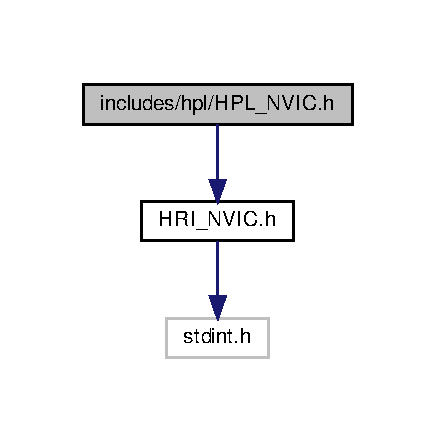
\includegraphics[width=209pt]{dc/d03/HPL__NVIC_8h__incl}
\end{center}
\end{figure}
Gráfico de los archivos que directa o indirectamente incluyen a este archivo\+:\nopagebreak
\begin{figure}[H]
\begin{center}
\leavevmode
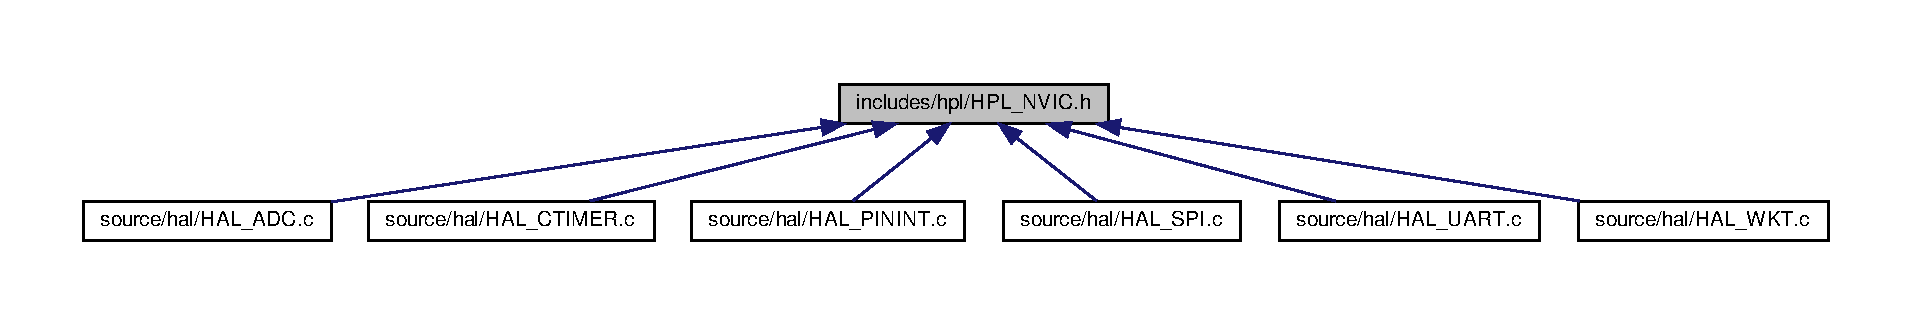
\includegraphics[width=350pt]{df/d29/HPL__NVIC_8h__dep__incl}
\end{center}
\end{figure}
\subsection*{Enumeraciones}
\begin{DoxyCompactItemize}
\item 
\mbox{\Hypertarget{HPL__NVIC_8h_a8a646e37498ef454b9145baea6e4ca04}\label{HPL__NVIC_8h_a8a646e37498ef454b9145baea6e4ca04}} 
enum {\bfseries N\+V\+I\+C\+\_\+irq\+\_\+sel\+\_\+en} \{ \newline
{\bfseries N\+V\+I\+C\+\_\+\+I\+R\+Q\+\_\+\+S\+E\+L\+\_\+\+S\+P\+I0} = 0, 
{\bfseries N\+V\+I\+C\+\_\+\+I\+R\+Q\+\_\+\+S\+E\+L\+\_\+\+S\+P\+I1}, 
{\bfseries N\+V\+I\+C\+\_\+\+I\+R\+Q\+\_\+\+S\+E\+L\+\_\+\+D\+A\+C0}, 
{\bfseries N\+V\+I\+C\+\_\+\+I\+R\+Q\+\_\+\+S\+E\+L\+\_\+\+U\+A\+R\+T0}, 
\newline
{\bfseries N\+V\+I\+C\+\_\+\+I\+R\+Q\+\_\+\+S\+E\+L\+\_\+\+U\+A\+R\+T1}, 
{\bfseries N\+V\+I\+C\+\_\+\+I\+R\+Q\+\_\+\+S\+E\+L\+\_\+\+U\+A\+R\+T2}, 
{\bfseries N\+V\+I\+C\+\_\+\+I\+R\+Q\+\_\+\+S\+E\+L\+\_\+\+I\+I\+C1} = 7, 
{\bfseries N\+V\+I\+C\+\_\+\+I\+R\+Q\+\_\+\+S\+E\+L\+\_\+\+I\+I\+C0}, 
\newline
{\bfseries N\+V\+I\+C\+\_\+\+I\+R\+Q\+\_\+\+S\+E\+L\+\_\+\+S\+CT}, 
{\bfseries N\+V\+I\+C\+\_\+\+I\+R\+Q\+\_\+\+S\+E\+L\+\_\+\+M\+RT}, 
{\bfseries N\+V\+I\+C\+\_\+\+I\+R\+Q\+\_\+\+S\+E\+L\+\_\+\+C\+M\+P\+\_\+\+C\+A\+PT}, 
{\bfseries N\+V\+I\+C\+\_\+\+I\+R\+Q\+\_\+\+S\+E\+L\+\_\+\+W\+DT}, 
\newline
{\bfseries N\+V\+I\+C\+\_\+\+I\+R\+Q\+\_\+\+S\+E\+L\+\_\+\+B\+OD}, 
{\bfseries N\+V\+I\+C\+\_\+\+I\+R\+Q\+\_\+\+S\+E\+L\+\_\+\+F\+L\+A\+SH}, 
{\bfseries N\+V\+I\+C\+\_\+\+I\+R\+Q\+\_\+\+S\+E\+L\+\_\+\+W\+KT}, 
{\bfseries N\+V\+I\+C\+\_\+\+I\+R\+Q\+\_\+\+S\+E\+L\+\_\+\+A\+D\+C\+\_\+\+S\+E\+QA}, 
\newline
{\bfseries N\+V\+I\+C\+\_\+\+I\+R\+Q\+\_\+\+S\+E\+L\+\_\+\+A\+D\+C\+\_\+\+S\+E\+QB}, 
{\bfseries N\+V\+I\+C\+\_\+\+I\+R\+Q\+\_\+\+S\+E\+L\+\_\+\+A\+D\+C\+\_\+\+T\+H\+C\+MP}, 
{\bfseries N\+V\+I\+C\+\_\+\+I\+R\+Q\+\_\+\+S\+E\+L\+\_\+\+A\+D\+C\+\_\+\+O\+VR}, 
{\bfseries N\+V\+I\+C\+\_\+\+I\+R\+Q\+\_\+\+S\+E\+L\+\_\+\+D\+MA}, 
\newline
{\bfseries N\+V\+I\+C\+\_\+\+I\+R\+Q\+\_\+\+S\+E\+L\+\_\+\+I\+I\+C2}, 
{\bfseries N\+V\+I\+C\+\_\+\+I\+R\+Q\+\_\+\+S\+E\+L\+\_\+\+I\+I\+C3}, 
{\bfseries N\+V\+I\+C\+\_\+\+I\+R\+Q\+\_\+\+S\+E\+L\+\_\+\+C\+T\+I\+M\+ER}, 
{\bfseries N\+V\+I\+C\+\_\+\+I\+R\+Q\+\_\+\+S\+E\+L\+\_\+\+P\+I\+N\+I\+N\+T0}, 
\newline
{\bfseries N\+V\+I\+C\+\_\+\+I\+R\+Q\+\_\+\+S\+E\+L\+\_\+\+P\+I\+N\+I\+N\+T1}, 
{\bfseries N\+V\+I\+C\+\_\+\+I\+R\+Q\+\_\+\+S\+E\+L\+\_\+\+P\+I\+N\+I\+N\+T2}, 
{\bfseries N\+V\+I\+C\+\_\+\+I\+R\+Q\+\_\+\+S\+E\+L\+\_\+\+P\+I\+N\+I\+N\+T3}, 
{\bfseries N\+V\+I\+C\+\_\+\+I\+R\+Q\+\_\+\+S\+E\+L\+\_\+\+P\+I\+N\+I\+N\+T4}, 
\newline
{\bfseries N\+V\+I\+C\+\_\+\+I\+R\+Q\+\_\+\+S\+E\+L\+\_\+\+P\+I\+N\+I\+N\+T5\+\_\+\+D\+A\+C1}, 
{\bfseries N\+V\+I\+C\+\_\+\+I\+R\+Q\+\_\+\+S\+E\+L\+\_\+\+P\+I\+N\+I\+N\+T6\+\_\+\+U\+A\+R\+T3}, 
{\bfseries N\+V\+I\+C\+\_\+\+I\+R\+Q\+\_\+\+S\+E\+L\+\_\+\+P\+I\+N\+I\+N\+T7\+\_\+\+U\+A\+R\+T4}
 \}
\item 
\mbox{\Hypertarget{HPL__NVIC_8h_aeed8d6a280176a9a66ada77d931c060a}\label{HPL__NVIC_8h_aeed8d6a280176a9a66ada77d931c060a}} 
enum {\bfseries N\+V\+I\+C\+\_\+irq\+\_\+priority\+\_\+en} \{ {\bfseries N\+V\+I\+C\+\_\+\+I\+R\+Q\+\_\+\+P\+R\+I\+O\+R\+I\+T\+Y\+\_\+\+H\+I\+G\+H\+E\+ST} = 0, 
{\bfseries N\+V\+I\+C\+\_\+\+I\+R\+Q\+\_\+\+P\+R\+I\+O\+R\+I\+T\+Y\+\_\+\+H\+I\+GH}, 
{\bfseries N\+V\+I\+C\+\_\+\+I\+R\+Q\+\_\+\+P\+R\+I\+O\+R\+I\+T\+Y\+\_\+\+L\+OW}, 
{\bfseries N\+V\+I\+C\+\_\+\+I\+R\+Q\+\_\+\+P\+R\+I\+O\+R\+I\+T\+Y\+\_\+\+L\+O\+W\+E\+ST}
 \}
\end{DoxyCompactItemize}
\subsection*{Funciones}
\begin{DoxyCompactItemize}
\item 
static void \hyperlink{HPL__NVIC_8h_a3a6688d8a4dcc4695ad03f75d0f4fd08}{N\+V\+I\+C\+\_\+enable\+\_\+interrupt} (N\+V\+I\+C\+\_\+irq\+\_\+sel\+\_\+en irq)
\begin{DoxyCompactList}\small\item\em Habilitacion de interrupciones. \end{DoxyCompactList}\item 
static void \hyperlink{HPL__NVIC_8h_a9b283278cc6e5f98105fb1b86c5a5089}{N\+V\+I\+C\+\_\+disable\+\_\+interrupt} (N\+V\+I\+C\+\_\+irq\+\_\+sel\+\_\+en irq)
\begin{DoxyCompactList}\small\item\em Inhabilitacion de interrupciones. \end{DoxyCompactList}\item 
static void \hyperlink{HPL__NVIC_8h_a4e5aa6d9c46ae7b494881b588e209204}{N\+V\+I\+C\+\_\+set\+\_\+pending\+\_\+interrupt} (N\+V\+I\+C\+\_\+irq\+\_\+sel\+\_\+en irq)
\begin{DoxyCompactList}\small\item\em Fijar interupcion pendiente por software. \end{DoxyCompactList}\item 
static void \hyperlink{HPL__NVIC_8h_a7fd778c0a80c14c4855031b68396c4cd}{N\+V\+I\+C\+\_\+clear\+\_\+pending\+\_\+interrupt} (N\+V\+I\+C\+\_\+irq\+\_\+sel\+\_\+en irq)
\begin{DoxyCompactList}\small\item\em Limpiar interupcion pendiente por software. \end{DoxyCompactList}\item 
static uint8\+\_\+t \hyperlink{HPL__NVIC_8h_a8d3f8c281acb042a3c06eb7db7a7b7ca}{N\+V\+I\+C\+\_\+get\+\_\+active\+\_\+interrupt} (N\+V\+I\+C\+\_\+irq\+\_\+sel\+\_\+en irq)
\begin{DoxyCompactList}\small\item\em Obtener estado de interrupcion. \end{DoxyCompactList}\item 
\mbox{\Hypertarget{HPL__NVIC_8h_aeb759124d5e366dae565b5320c8b3355}\label{HPL__NVIC_8h_aeb759124d5e366dae565b5320c8b3355}} 
static void {\bfseries N\+V\+I\+C\+\_\+set\+\_\+irq\+\_\+priority} (N\+V\+I\+C\+\_\+irq\+\_\+sel\+\_\+en irq, N\+V\+I\+C\+\_\+irq\+\_\+priority\+\_\+en priority)
\end{DoxyCompactItemize}
\subsection*{Variables}
\begin{DoxyCompactItemize}
\item 
\mbox{\Hypertarget{HPL__NVIC_8h_a8d2cecc9010fc7e5fe2d37938628b55a}\label{HPL__NVIC_8h_a8d2cecc9010fc7e5fe2d37938628b55a}} 
volatile \hyperlink{HRI__NVIC_8h_de/df9/structNVIC__per__t}{N\+V\+I\+C\+\_\+per\+\_\+t} $\ast$const \hyperlink{HPL__NVIC_8h_a8d2cecc9010fc7e5fe2d37938628b55a}{N\+V\+IC}
\begin{DoxyCompactList}\small\item\em Periferico N\+V\+IC. \end{DoxyCompactList}\end{DoxyCompactItemize}


\subsection{Descripción detallada}
Declaraciones a nivel de abstraccion de periferico del N\+V\+IC (L\+P\+C845) 

\begin{DoxyAuthor}{Autor}
Augusto Santini 
\end{DoxyAuthor}
\begin{DoxyDate}{Fecha}
3/2020 
\end{DoxyDate}
\begin{DoxyVersion}{Versión}
1.\+0 
\end{DoxyVersion}


\subsection{Documentación de las funciones}
\mbox{\Hypertarget{HPL__NVIC_8h_a3a6688d8a4dcc4695ad03f75d0f4fd08}\label{HPL__NVIC_8h_a3a6688d8a4dcc4695ad03f75d0f4fd08}} 
\index{H\+P\+L\+\_\+\+N\+V\+I\+C.\+h@{H\+P\+L\+\_\+\+N\+V\+I\+C.\+h}!N\+V\+I\+C\+\_\+enable\+\_\+interrupt@{N\+V\+I\+C\+\_\+enable\+\_\+interrupt}}
\index{N\+V\+I\+C\+\_\+enable\+\_\+interrupt@{N\+V\+I\+C\+\_\+enable\+\_\+interrupt}!H\+P\+L\+\_\+\+N\+V\+I\+C.\+h@{H\+P\+L\+\_\+\+N\+V\+I\+C.\+h}}
\subsubsection{\texorpdfstring{N\+V\+I\+C\+\_\+enable\+\_\+interrupt()}{NVIC\_enable\_interrupt()}}
{\footnotesize\ttfamily static void N\+V\+I\+C\+\_\+enable\+\_\+interrupt (\begin{DoxyParamCaption}\item[{N\+V\+I\+C\+\_\+irq\+\_\+sel\+\_\+en}]{irq }\end{DoxyParamCaption})\hspace{0.3cm}{\ttfamily [inline]}, {\ttfamily [static]}}



Habilitacion de interrupciones. 


\begin{DoxyParams}[1]{Parámetros}
\mbox{\tt in}  & {\em irq} & Seleccion de fuente de interrupcion \\
\hline
\end{DoxyParams}
\mbox{\Hypertarget{HPL__NVIC_8h_a9b283278cc6e5f98105fb1b86c5a5089}\label{HPL__NVIC_8h_a9b283278cc6e5f98105fb1b86c5a5089}} 
\index{H\+P\+L\+\_\+\+N\+V\+I\+C.\+h@{H\+P\+L\+\_\+\+N\+V\+I\+C.\+h}!N\+V\+I\+C\+\_\+disable\+\_\+interrupt@{N\+V\+I\+C\+\_\+disable\+\_\+interrupt}}
\index{N\+V\+I\+C\+\_\+disable\+\_\+interrupt@{N\+V\+I\+C\+\_\+disable\+\_\+interrupt}!H\+P\+L\+\_\+\+N\+V\+I\+C.\+h@{H\+P\+L\+\_\+\+N\+V\+I\+C.\+h}}
\subsubsection{\texorpdfstring{N\+V\+I\+C\+\_\+disable\+\_\+interrupt()}{NVIC\_disable\_interrupt()}}
{\footnotesize\ttfamily static void N\+V\+I\+C\+\_\+disable\+\_\+interrupt (\begin{DoxyParamCaption}\item[{N\+V\+I\+C\+\_\+irq\+\_\+sel\+\_\+en}]{irq }\end{DoxyParamCaption})\hspace{0.3cm}{\ttfamily [inline]}, {\ttfamily [static]}}



Inhabilitacion de interrupciones. 


\begin{DoxyParams}[1]{Parámetros}
\mbox{\tt in}  & {\em irq} & Seleccion de fuente de interrupcion \\
\hline
\end{DoxyParams}
\mbox{\Hypertarget{HPL__NVIC_8h_a4e5aa6d9c46ae7b494881b588e209204}\label{HPL__NVIC_8h_a4e5aa6d9c46ae7b494881b588e209204}} 
\index{H\+P\+L\+\_\+\+N\+V\+I\+C.\+h@{H\+P\+L\+\_\+\+N\+V\+I\+C.\+h}!N\+V\+I\+C\+\_\+set\+\_\+pending\+\_\+interrupt@{N\+V\+I\+C\+\_\+set\+\_\+pending\+\_\+interrupt}}
\index{N\+V\+I\+C\+\_\+set\+\_\+pending\+\_\+interrupt@{N\+V\+I\+C\+\_\+set\+\_\+pending\+\_\+interrupt}!H\+P\+L\+\_\+\+N\+V\+I\+C.\+h@{H\+P\+L\+\_\+\+N\+V\+I\+C.\+h}}
\subsubsection{\texorpdfstring{N\+V\+I\+C\+\_\+set\+\_\+pending\+\_\+interrupt()}{NVIC\_set\_pending\_interrupt()}}
{\footnotesize\ttfamily static void N\+V\+I\+C\+\_\+set\+\_\+pending\+\_\+interrupt (\begin{DoxyParamCaption}\item[{N\+V\+I\+C\+\_\+irq\+\_\+sel\+\_\+en}]{irq }\end{DoxyParamCaption})\hspace{0.3cm}{\ttfamily [inline]}, {\ttfamily [static]}}



Fijar interupcion pendiente por software. 


\begin{DoxyParams}[1]{Parámetros}
\mbox{\tt in}  & {\em irq} & Seleccion de fuente de interrupcion \\
\hline
\end{DoxyParams}
\mbox{\Hypertarget{HPL__NVIC_8h_a7fd778c0a80c14c4855031b68396c4cd}\label{HPL__NVIC_8h_a7fd778c0a80c14c4855031b68396c4cd}} 
\index{H\+P\+L\+\_\+\+N\+V\+I\+C.\+h@{H\+P\+L\+\_\+\+N\+V\+I\+C.\+h}!N\+V\+I\+C\+\_\+clear\+\_\+pending\+\_\+interrupt@{N\+V\+I\+C\+\_\+clear\+\_\+pending\+\_\+interrupt}}
\index{N\+V\+I\+C\+\_\+clear\+\_\+pending\+\_\+interrupt@{N\+V\+I\+C\+\_\+clear\+\_\+pending\+\_\+interrupt}!H\+P\+L\+\_\+\+N\+V\+I\+C.\+h@{H\+P\+L\+\_\+\+N\+V\+I\+C.\+h}}
\subsubsection{\texorpdfstring{N\+V\+I\+C\+\_\+clear\+\_\+pending\+\_\+interrupt()}{NVIC\_clear\_pending\_interrupt()}}
{\footnotesize\ttfamily static void N\+V\+I\+C\+\_\+clear\+\_\+pending\+\_\+interrupt (\begin{DoxyParamCaption}\item[{N\+V\+I\+C\+\_\+irq\+\_\+sel\+\_\+en}]{irq }\end{DoxyParamCaption})\hspace{0.3cm}{\ttfamily [inline]}, {\ttfamily [static]}}



Limpiar interupcion pendiente por software. 


\begin{DoxyParams}[1]{Parámetros}
\mbox{\tt in}  & {\em irq} & Seleccion de fuente de interrupcion \\
\hline
\end{DoxyParams}
\mbox{\Hypertarget{HPL__NVIC_8h_a8d3f8c281acb042a3c06eb7db7a7b7ca}\label{HPL__NVIC_8h_a8d3f8c281acb042a3c06eb7db7a7b7ca}} 
\index{H\+P\+L\+\_\+\+N\+V\+I\+C.\+h@{H\+P\+L\+\_\+\+N\+V\+I\+C.\+h}!N\+V\+I\+C\+\_\+get\+\_\+active\+\_\+interrupt@{N\+V\+I\+C\+\_\+get\+\_\+active\+\_\+interrupt}}
\index{N\+V\+I\+C\+\_\+get\+\_\+active\+\_\+interrupt@{N\+V\+I\+C\+\_\+get\+\_\+active\+\_\+interrupt}!H\+P\+L\+\_\+\+N\+V\+I\+C.\+h@{H\+P\+L\+\_\+\+N\+V\+I\+C.\+h}}
\subsubsection{\texorpdfstring{N\+V\+I\+C\+\_\+get\+\_\+active\+\_\+interrupt()}{NVIC\_get\_active\_interrupt()}}
{\footnotesize\ttfamily static uint8\+\_\+t N\+V\+I\+C\+\_\+get\+\_\+active\+\_\+interrupt (\begin{DoxyParamCaption}\item[{N\+V\+I\+C\+\_\+irq\+\_\+sel\+\_\+en}]{irq }\end{DoxyParamCaption})\hspace{0.3cm}{\ttfamily [inline]}, {\ttfamily [static]}}



Obtener estado de interrupcion. 


\begin{DoxyParams}[1]{Parámetros}
\mbox{\tt in}  & {\em irq} & Seleccion de fuente de interrupcion \\
\hline
\end{DoxyParams}
\begin{DoxyReturn}{Devuelve}
Si la interrupcion estaba activa devuelve 1, caso contrario devuelve 0 
\end{DoxyReturn}

\hypertarget{HPL__PININT_8h}{}\section{Referencia del Archivo includes/hpl/\+H\+P\+L\+\_\+\+P\+I\+N\+I\+NT.h}
\label{HPL__PININT_8h}\index{includes/hpl/\+H\+P\+L\+\_\+\+P\+I\+N\+I\+N\+T.\+h@{includes/hpl/\+H\+P\+L\+\_\+\+P\+I\+N\+I\+N\+T.\+h}}


Declaraciones a nivel de abstraccion de periferico del P\+I\+N\+I\+NT (L\+P\+C845)  


{\ttfamily \#include $<$H\+R\+I\+\_\+\+P\+I\+N\+I\+N\+T.\+h$>$}\newline
Dependencia gráfica adjunta para H\+P\+L\+\_\+\+P\+I\+N\+I\+N\+T.\+h\+:\nopagebreak
\begin{figure}[H]
\begin{center}
\leavevmode
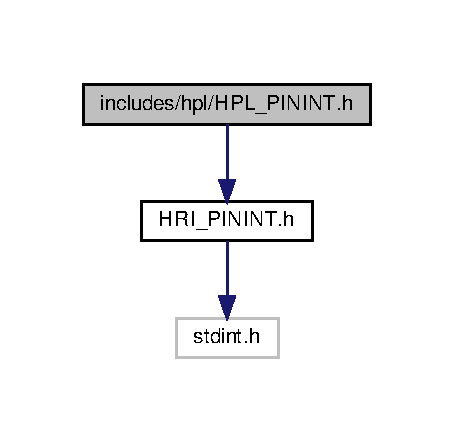
\includegraphics[width=218pt]{HPL__PININT_8h__incl}
\end{center}
\end{figure}
Gráfico de los archivos que directa o indirectamente incluyen a este archivo\+:\nopagebreak
\begin{figure}[H]
\begin{center}
\leavevmode
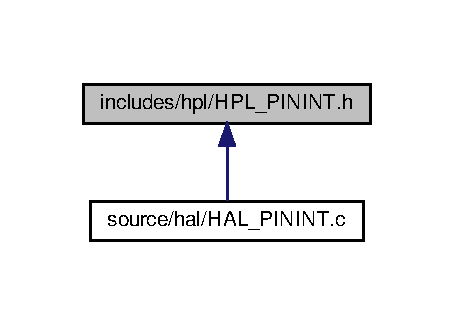
\includegraphics[width=218pt]{HPL__PININT_8h__dep__incl}
\end{center}
\end{figure}
\subsection*{Enumeraciones}
\begin{DoxyCompactItemize}
\item 
\mbox{\Hypertarget{HPL__PININT_8h_afedddf6149b1ef6f34ed9c34cf7956a2}\label{HPL__PININT_8h_afedddf6149b1ef6f34ed9c34cf7956a2}} 
enum {\bfseries P\+I\+N\+I\+N\+T\+\_\+interrupt\+\_\+mode\+\_\+en} \{ {\bfseries P\+I\+N\+I\+N\+T\+\_\+\+I\+N\+T\+E\+R\+R\+U\+P\+T\+\_\+\+M\+O\+D\+E\+\_\+\+E\+D\+GE} = 0, 
{\bfseries P\+I\+N\+I\+N\+T\+\_\+\+I\+N\+T\+E\+R\+R\+U\+P\+T\+\_\+\+M\+O\+D\+E\+\_\+\+L\+E\+V\+EL}
 \}
\item 
\mbox{\Hypertarget{HPL__PININT_8h_a3c335d713fff3fd7481029d6966225fe}\label{HPL__PININT_8h_a3c335d713fff3fd7481029d6966225fe}} 
enum {\bfseries P\+I\+N\+I\+N\+T\+\_\+match\+\_\+contribution\+\_\+en} \{ \newline
{\bfseries P\+I\+N\+I\+N\+T\+\_\+\+M\+A\+T\+C\+H\+\_\+\+C\+O\+N\+T\+R\+I\+B\+U\+T\+I\+O\+N\+\_\+\+C\+O\+N\+S\+T\+A\+N\+T\+\_\+\+H\+I\+GH} = 0, 
{\bfseries P\+I\+N\+I\+N\+T\+\_\+\+M\+A\+T\+C\+H\+\_\+\+C\+O\+N\+T\+R\+I\+B\+U\+T\+I\+O\+N\+\_\+\+S\+T\+I\+C\+K\+Y\+\_\+\+R\+I\+S\+I\+N\+G\+\_\+\+E\+D\+GE}, 
{\bfseries P\+I\+N\+I\+N\+T\+\_\+\+M\+A\+T\+C\+H\+\_\+\+C\+O\+N\+T\+R\+I\+B\+U\+T\+I\+O\+N\+\_\+\+S\+T\+I\+C\+K\+Y\+\_\+\+F\+A\+L\+L\+I\+N\+G\+\_\+\+E\+D\+GE}, 
{\bfseries P\+I\+N\+I\+N\+T\+\_\+\+M\+A\+T\+C\+H\+\_\+\+C\+O\+N\+T\+R\+I\+B\+U\+T\+I\+O\+N\+\_\+\+S\+T\+I\+C\+K\+Y\+\_\+\+R\+I\+S\+I\+N\+G\+\_\+\+O\+R\+\_\+\+F\+A\+L\+L\+I\+N\+G\+\_\+\+E\+D\+GE}, 
\newline
{\bfseries P\+I\+N\+I\+N\+T\+\_\+\+M\+A\+T\+C\+H\+\_\+\+C\+O\+N\+T\+R\+I\+B\+U\+T\+I\+O\+N\+\_\+\+H\+I\+G\+H\+\_\+\+L\+E\+V\+EL}, 
{\bfseries P\+I\+N\+I\+N\+T\+\_\+\+M\+A\+T\+C\+H\+\_\+\+C\+O\+N\+T\+R\+I\+B\+U\+T\+I\+O\+N\+\_\+\+L\+O\+W\+\_\+\+L\+E\+V\+EL}, 
{\bfseries P\+I\+N\+I\+N\+T\+\_\+\+M\+A\+T\+C\+H\+\_\+\+C\+O\+N\+T\+R\+I\+B\+U\+T\+I\+O\+N\+\_\+\+C\+O\+N\+S\+T\+A\+N\+T\+\_\+0}, 
{\bfseries P\+I\+N\+I\+N\+T\+\_\+\+M\+A\+T\+C\+H\+\_\+\+C\+O\+N\+T\+R\+I\+B\+U\+T\+I\+O\+N\+\_\+\+E\+V\+E\+NT}
 \}
\end{DoxyCompactItemize}
\subsection*{Funciones}
\begin{DoxyCompactItemize}
\item 
static void \hyperlink{HPL__PININT_8h_ae34c3b1c0619c0f7213bff15423fd51f}{P\+I\+N\+I\+N\+T\+\_\+set\+\_\+interrupt\+\_\+mode} (uint8\+\_\+t channel, P\+I\+N\+I\+N\+T\+\_\+interrupt\+\_\+mode\+\_\+en mode)
\begin{DoxyCompactList}\small\item\em Configurar sensibilidad a nivel/flanco. \end{DoxyCompactList}\item 
static P\+I\+N\+I\+N\+T\+\_\+interrupt\+\_\+mode\+\_\+en \hyperlink{HPL__PININT_8h_aaad4342b1f8893a5905667a6edccc996}{P\+I\+N\+I\+N\+T\+\_\+get\+\_\+interrupt\+\_\+mode} (uint8\+\_\+t channel)
\begin{DoxyCompactList}\small\item\em Obtener configuracion de modo de un canal. \end{DoxyCompactList}\item 
static void \hyperlink{HPL__PININT_8h_a88365ad65b107b71109708196d04630c}{P\+I\+N\+I\+N\+T\+\_\+enable\+\_\+rising\+\_\+edge} (uint8\+\_\+t channel)
\begin{DoxyCompactList}\small\item\em Habilitar detecciones por flanco ascendente. \end{DoxyCompactList}\item 
static void \hyperlink{HPL__PININT_8h_a45e8327b0094015a313a0972e772f288}{P\+I\+N\+I\+N\+T\+\_\+disable\+\_\+rising\+\_\+edge} (uint8\+\_\+t channel)
\begin{DoxyCompactList}\small\item\em Inhabilitar detecciones por flanco ascendente. \end{DoxyCompactList}\item 
static void \hyperlink{HPL__PININT_8h_a9916a55fa487d0421d655ddb88d7c2e7}{P\+I\+N\+I\+N\+T\+\_\+enable\+\_\+falling\+\_\+edge} (uint8\+\_\+t channel)
\begin{DoxyCompactList}\small\item\em Habilitar detecciones por flanco descendente. \end{DoxyCompactList}\item 
static void \hyperlink{HPL__PININT_8h_ac047361d7b55f37667b9baa2ddcbc2bb}{P\+I\+N\+I\+N\+T\+\_\+disable\+\_\+falling\+\_\+edge} (uint8\+\_\+t channel)
\begin{DoxyCompactList}\small\item\em Inhabilitar detecciones por flanco descendente. \end{DoxyCompactList}\item 
static void \hyperlink{HPL__PININT_8h_a4c6b2f70c6eab17a4b568b676f9b76ae}{P\+I\+N\+I\+N\+T\+\_\+enable\+\_\+high\+\_\+level} (uint8\+\_\+t channel)
\begin{DoxyCompactList}\small\item\em Habilitar detecciones por nivel alto. \end{DoxyCompactList}\item 
static void \hyperlink{HPL__PININT_8h_ac73003895b3499d9f992d29bb94d3c2a}{P\+I\+N\+I\+N\+T\+\_\+disable\+\_\+high\+\_\+level} (uint8\+\_\+t channel)
\begin{DoxyCompactList}\small\item\em Inhabilitar detecciones por flanco ascendente. \end{DoxyCompactList}\item 
static uint8\+\_\+t \hyperlink{HPL__PININT_8h_aefe7fb5a435fb1443119d794ad89e40a}{P\+I\+N\+I\+N\+T\+\_\+get\+\_\+rising\+\_\+edge\+\_\+active} (void)
\begin{DoxyCompactList}\small\item\em Obtener interrupciones activas por flanco ascendente. \end{DoxyCompactList}\item 
static uint8\+\_\+t \hyperlink{HPL__PININT_8h_a893f958b5ba47d1ad53b858162449df6}{P\+I\+N\+I\+N\+T\+\_\+get\+\_\+falling\+\_\+edge\+\_\+active} (void)
\begin{DoxyCompactList}\small\item\em Obtener interrupciones activas por flanco descendente. \end{DoxyCompactList}\item 
static uint8\+\_\+t \hyperlink{HPL__PININT_8h_a82705d128a938c409cfc92798252c5d9}{P\+I\+N\+I\+N\+T\+\_\+get\+\_\+level\+\_\+active} (void)
\begin{DoxyCompactList}\small\item\em Obtener interrupciones activas por nivel. \end{DoxyCompactList}\item 
static void \hyperlink{HPL__PININT_8h_ac569d34a3e59a4b4436215a9eea81dc4}{P\+I\+N\+I\+N\+T\+\_\+clear\+\_\+edge\+\_\+level\+\_\+irq} (uint8\+\_\+t channel)
\begin{DoxyCompactList}\small\item\em Limpiar flag de interrupcion por flanco. \end{DoxyCompactList}\item 
static void \hyperlink{HPL__PININT_8h_a1c21251810ad00cbb1c7e74990891da1}{P\+I\+N\+I\+N\+T\+\_\+toggle\+\_\+active\+\_\+level} (uint8\+\_\+t channel)
\begin{DoxyCompactList}\small\item\em Invertir nivel activo de itnerrupcion por nivel. \end{DoxyCompactList}\item 
\mbox{\Hypertarget{HPL__PININT_8h_afeb4897a5e8224d32cb9ca4c157ea4b6}\label{HPL__PININT_8h_afeb4897a5e8224d32cb9ca4c157ea4b6}} 
static void \hyperlink{HPL__PININT_8h_afeb4897a5e8224d32cb9ca4c157ea4b6}{P\+I\+N\+I\+N\+T\+\_\+enable\+\_\+pattern\+\_\+match} (void)
\begin{DoxyCompactList}\small\item\em Habilita el funcionamiento del pattern match engine (inhabilita P\+I\+N\+I\+NT) \end{DoxyCompactList}\item 
\mbox{\Hypertarget{HPL__PININT_8h_aa982840cccebe4de0acc33067e964cbf}\label{HPL__PININT_8h_aa982840cccebe4de0acc33067e964cbf}} 
static void \hyperlink{HPL__PININT_8h_aa982840cccebe4de0acc33067e964cbf}{P\+I\+N\+I\+N\+T\+\_\+disable\+\_\+pattern\+\_\+match} (void)
\begin{DoxyCompactList}\small\item\em Inhabilita el funcionamiento del pattern match engine (habilita P\+I\+N\+I\+NT) \end{DoxyCompactList}\item 
\mbox{\Hypertarget{HPL__PININT_8h_ae16bcf342a686057e6d01242c2cb1c5d}\label{HPL__PININT_8h_ae16bcf342a686057e6d01242c2cb1c5d}} 
static void \hyperlink{HPL__PININT_8h_ae16bcf342a686057e6d01242c2cb1c5d}{P\+I\+N\+I\+N\+T\+\_\+enable\+\_\+\+R\+X\+EV} (void)
\begin{DoxyCompactList}\small\item\em Habilita la salida de R\+X\+EV. \end{DoxyCompactList}\item 
\mbox{\Hypertarget{HPL__PININT_8h_ac698eb44fa9eba8405fa5a9c8416d8de}\label{HPL__PININT_8h_ac698eb44fa9eba8405fa5a9c8416d8de}} 
static void \hyperlink{HPL__PININT_8h_ac698eb44fa9eba8405fa5a9c8416d8de}{P\+I\+N\+I\+N\+T\+\_\+disable\+\_\+\+R\+X\+EV} (void)
\begin{DoxyCompactList}\small\item\em Inhabilita la salida de R\+X\+EV. \end{DoxyCompactList}\item 
static uint8\+\_\+t \hyperlink{HPL__PININT_8h_ab9ac187bcef8fb438cd11ea516964857}{P\+I\+N\+I\+N\+T\+\_\+get\+\_\+pattern\+\_\+match\+\_\+state} (void)
\begin{DoxyCompactList}\small\item\em Obtener estado actual del pattern match. \end{DoxyCompactList}\item 
static void \hyperlink{HPL__PININT_8h_ae3fbc54806d88ced3e2aa0309d1f39a4}{P\+I\+N\+I\+N\+T\+\_\+config\+\_\+pattern\+\_\+match\+\_\+source} (uint8\+\_\+t channel, uint8\+\_\+t slice)
\begin{DoxyCompactList}\small\item\em Configuracion de las fuentes del pattern match. \end{DoxyCompactList}\item 
static void \hyperlink{HPL__PININT_8h_a3817ddf0cabe27506a684f133a39c1e6}{P\+I\+N\+I\+T\+N\+\_\+enable\+\_\+slice\+\_\+as\+\_\+endpoint} (uint8\+\_\+t slice)
\begin{DoxyCompactList}\small\item\em Habilitar slice como endpoint. \end{DoxyCompactList}\item 
static void \hyperlink{HPL__PININT_8h_a332e6ff1bbb428f78f85381d80c26c82}{P\+I\+N\+I\+T\+N\+\_\+disable\+\_\+slice\+\_\+as\+\_\+endpoint} (uint8\+\_\+t slice)
\begin{DoxyCompactList}\small\item\em Inhabilitar slice como endpoint. \end{DoxyCompactList}\item 
static void \hyperlink{HPL__PININT_8h_a18adbbe7e860455b270984b9b95ee000}{P\+I\+N\+I\+T\+N\+\_\+config\+\_\+slice\+\_\+mode} (uint8\+\_\+t slice, P\+I\+N\+I\+N\+T\+\_\+match\+\_\+contribution\+\_\+en mode)
\begin{DoxyCompactList}\small\item\em Configurar modo del slice. \end{DoxyCompactList}\end{DoxyCompactItemize}
\subsection*{Variables}
\begin{DoxyCompactItemize}
\item 
\mbox{\Hypertarget{HPL__PININT_8h_a26d606920082b585bdd0bd0279fe6177}\label{HPL__PININT_8h_a26d606920082b585bdd0bd0279fe6177}} 
volatile \hyperlink{HRI__PININT_8h_structPININT__per__t}{P\+I\+N\+I\+N\+T\+\_\+per\+\_\+t} $\ast$const \hyperlink{HPL__PININT_8h_a26d606920082b585bdd0bd0279fe6177}{P\+I\+N\+I\+NT}
\begin{DoxyCompactList}\small\item\em Periferico P\+I\+N\+I\+NT. \end{DoxyCompactList}\end{DoxyCompactItemize}


\subsection{Descripción detallada}
Declaraciones a nivel de abstraccion de periferico del P\+I\+N\+I\+NT (L\+P\+C845) 

\begin{DoxyAuthor}{Autor}
Augusto Santini 
\end{DoxyAuthor}
\begin{DoxyDate}{Fecha}
6/2019 
\end{DoxyDate}
\begin{DoxyVersion}{Versión}
1.\+0 
\end{DoxyVersion}


\subsection{Documentación de las funciones}
\mbox{\Hypertarget{HPL__PININT_8h_ae34c3b1c0619c0f7213bff15423fd51f}\label{HPL__PININT_8h_ae34c3b1c0619c0f7213bff15423fd51f}} 
\index{H\+P\+L\+\_\+\+P\+I\+N\+I\+N\+T.\+h@{H\+P\+L\+\_\+\+P\+I\+N\+I\+N\+T.\+h}!P\+I\+N\+I\+N\+T\+\_\+set\+\_\+interrupt\+\_\+mode@{P\+I\+N\+I\+N\+T\+\_\+set\+\_\+interrupt\+\_\+mode}}
\index{P\+I\+N\+I\+N\+T\+\_\+set\+\_\+interrupt\+\_\+mode@{P\+I\+N\+I\+N\+T\+\_\+set\+\_\+interrupt\+\_\+mode}!H\+P\+L\+\_\+\+P\+I\+N\+I\+N\+T.\+h@{H\+P\+L\+\_\+\+P\+I\+N\+I\+N\+T.\+h}}
\subsubsection{\texorpdfstring{P\+I\+N\+I\+N\+T\+\_\+set\+\_\+interrupt\+\_\+mode()}{PININT\_set\_interrupt\_mode()}}
{\footnotesize\ttfamily static void P\+I\+N\+I\+N\+T\+\_\+set\+\_\+interrupt\+\_\+mode (\begin{DoxyParamCaption}\item[{uint8\+\_\+t}]{channel,  }\item[{P\+I\+N\+I\+N\+T\+\_\+interrupt\+\_\+mode\+\_\+en}]{mode }\end{DoxyParamCaption})\hspace{0.3cm}{\ttfamily [inline]}, {\ttfamily [static]}}



Configurar sensibilidad a nivel/flanco. 


\begin{DoxyParams}[1]{Parámetros}
\mbox{\tt in}  & {\em channel} & Canal a configurar \\
\hline
\mbox{\tt in}  & {\em mode} & Modo deseado \\
\hline
\end{DoxyParams}
\mbox{\Hypertarget{HPL__PININT_8h_aaad4342b1f8893a5905667a6edccc996}\label{HPL__PININT_8h_aaad4342b1f8893a5905667a6edccc996}} 
\index{H\+P\+L\+\_\+\+P\+I\+N\+I\+N\+T.\+h@{H\+P\+L\+\_\+\+P\+I\+N\+I\+N\+T.\+h}!P\+I\+N\+I\+N\+T\+\_\+get\+\_\+interrupt\+\_\+mode@{P\+I\+N\+I\+N\+T\+\_\+get\+\_\+interrupt\+\_\+mode}}
\index{P\+I\+N\+I\+N\+T\+\_\+get\+\_\+interrupt\+\_\+mode@{P\+I\+N\+I\+N\+T\+\_\+get\+\_\+interrupt\+\_\+mode}!H\+P\+L\+\_\+\+P\+I\+N\+I\+N\+T.\+h@{H\+P\+L\+\_\+\+P\+I\+N\+I\+N\+T.\+h}}
\subsubsection{\texorpdfstring{P\+I\+N\+I\+N\+T\+\_\+get\+\_\+interrupt\+\_\+mode()}{PININT\_get\_interrupt\_mode()}}
{\footnotesize\ttfamily static P\+I\+N\+I\+N\+T\+\_\+interrupt\+\_\+mode\+\_\+en P\+I\+N\+I\+N\+T\+\_\+get\+\_\+interrupt\+\_\+mode (\begin{DoxyParamCaption}\item[{uint8\+\_\+t}]{channel }\end{DoxyParamCaption})\hspace{0.3cm}{\ttfamily [inline]}, {\ttfamily [static]}}



Obtener configuracion de modo de un canal. 


\begin{DoxyParams}[1]{Parámetros}
\mbox{\tt in}  & {\em channel} & Canal a consultar \\
\hline
\end{DoxyParams}
\begin{DoxyReturn}{Devuelve}
Modo configurado para el canal 
\end{DoxyReturn}
\mbox{\Hypertarget{HPL__PININT_8h_a88365ad65b107b71109708196d04630c}\label{HPL__PININT_8h_a88365ad65b107b71109708196d04630c}} 
\index{H\+P\+L\+\_\+\+P\+I\+N\+I\+N\+T.\+h@{H\+P\+L\+\_\+\+P\+I\+N\+I\+N\+T.\+h}!P\+I\+N\+I\+N\+T\+\_\+enable\+\_\+rising\+\_\+edge@{P\+I\+N\+I\+N\+T\+\_\+enable\+\_\+rising\+\_\+edge}}
\index{P\+I\+N\+I\+N\+T\+\_\+enable\+\_\+rising\+\_\+edge@{P\+I\+N\+I\+N\+T\+\_\+enable\+\_\+rising\+\_\+edge}!H\+P\+L\+\_\+\+P\+I\+N\+I\+N\+T.\+h@{H\+P\+L\+\_\+\+P\+I\+N\+I\+N\+T.\+h}}
\subsubsection{\texorpdfstring{P\+I\+N\+I\+N\+T\+\_\+enable\+\_\+rising\+\_\+edge()}{PININT\_enable\_rising\_edge()}}
{\footnotesize\ttfamily static void P\+I\+N\+I\+N\+T\+\_\+enable\+\_\+rising\+\_\+edge (\begin{DoxyParamCaption}\item[{uint8\+\_\+t}]{channel }\end{DoxyParamCaption})\hspace{0.3cm}{\ttfamily [inline]}, {\ttfamily [static]}}



Habilitar detecciones por flanco ascendente. 


\begin{DoxyParams}[1]{Parámetros}
\mbox{\tt in}  & {\em channel} & Canal deseado \\
\hline
\end{DoxyParams}
\mbox{\Hypertarget{HPL__PININT_8h_a45e8327b0094015a313a0972e772f288}\label{HPL__PININT_8h_a45e8327b0094015a313a0972e772f288}} 
\index{H\+P\+L\+\_\+\+P\+I\+N\+I\+N\+T.\+h@{H\+P\+L\+\_\+\+P\+I\+N\+I\+N\+T.\+h}!P\+I\+N\+I\+N\+T\+\_\+disable\+\_\+rising\+\_\+edge@{P\+I\+N\+I\+N\+T\+\_\+disable\+\_\+rising\+\_\+edge}}
\index{P\+I\+N\+I\+N\+T\+\_\+disable\+\_\+rising\+\_\+edge@{P\+I\+N\+I\+N\+T\+\_\+disable\+\_\+rising\+\_\+edge}!H\+P\+L\+\_\+\+P\+I\+N\+I\+N\+T.\+h@{H\+P\+L\+\_\+\+P\+I\+N\+I\+N\+T.\+h}}
\subsubsection{\texorpdfstring{P\+I\+N\+I\+N\+T\+\_\+disable\+\_\+rising\+\_\+edge()}{PININT\_disable\_rising\_edge()}}
{\footnotesize\ttfamily static void P\+I\+N\+I\+N\+T\+\_\+disable\+\_\+rising\+\_\+edge (\begin{DoxyParamCaption}\item[{uint8\+\_\+t}]{channel }\end{DoxyParamCaption})\hspace{0.3cm}{\ttfamily [inline]}, {\ttfamily [static]}}



Inhabilitar detecciones por flanco ascendente. 


\begin{DoxyParams}[1]{Parámetros}
\mbox{\tt in}  & {\em channel} & Canal deseado \\
\hline
\end{DoxyParams}
\mbox{\Hypertarget{HPL__PININT_8h_a9916a55fa487d0421d655ddb88d7c2e7}\label{HPL__PININT_8h_a9916a55fa487d0421d655ddb88d7c2e7}} 
\index{H\+P\+L\+\_\+\+P\+I\+N\+I\+N\+T.\+h@{H\+P\+L\+\_\+\+P\+I\+N\+I\+N\+T.\+h}!P\+I\+N\+I\+N\+T\+\_\+enable\+\_\+falling\+\_\+edge@{P\+I\+N\+I\+N\+T\+\_\+enable\+\_\+falling\+\_\+edge}}
\index{P\+I\+N\+I\+N\+T\+\_\+enable\+\_\+falling\+\_\+edge@{P\+I\+N\+I\+N\+T\+\_\+enable\+\_\+falling\+\_\+edge}!H\+P\+L\+\_\+\+P\+I\+N\+I\+N\+T.\+h@{H\+P\+L\+\_\+\+P\+I\+N\+I\+N\+T.\+h}}
\subsubsection{\texorpdfstring{P\+I\+N\+I\+N\+T\+\_\+enable\+\_\+falling\+\_\+edge()}{PININT\_enable\_falling\_edge()}}
{\footnotesize\ttfamily static void P\+I\+N\+I\+N\+T\+\_\+enable\+\_\+falling\+\_\+edge (\begin{DoxyParamCaption}\item[{uint8\+\_\+t}]{channel }\end{DoxyParamCaption})\hspace{0.3cm}{\ttfamily [inline]}, {\ttfamily [static]}}



Habilitar detecciones por flanco descendente. 


\begin{DoxyParams}[1]{Parámetros}
\mbox{\tt in}  & {\em channel} & Canal deseado \\
\hline
\end{DoxyParams}
\mbox{\Hypertarget{HPL__PININT_8h_ac047361d7b55f37667b9baa2ddcbc2bb}\label{HPL__PININT_8h_ac047361d7b55f37667b9baa2ddcbc2bb}} 
\index{H\+P\+L\+\_\+\+P\+I\+N\+I\+N\+T.\+h@{H\+P\+L\+\_\+\+P\+I\+N\+I\+N\+T.\+h}!P\+I\+N\+I\+N\+T\+\_\+disable\+\_\+falling\+\_\+edge@{P\+I\+N\+I\+N\+T\+\_\+disable\+\_\+falling\+\_\+edge}}
\index{P\+I\+N\+I\+N\+T\+\_\+disable\+\_\+falling\+\_\+edge@{P\+I\+N\+I\+N\+T\+\_\+disable\+\_\+falling\+\_\+edge}!H\+P\+L\+\_\+\+P\+I\+N\+I\+N\+T.\+h@{H\+P\+L\+\_\+\+P\+I\+N\+I\+N\+T.\+h}}
\subsubsection{\texorpdfstring{P\+I\+N\+I\+N\+T\+\_\+disable\+\_\+falling\+\_\+edge()}{PININT\_disable\_falling\_edge()}}
{\footnotesize\ttfamily static void P\+I\+N\+I\+N\+T\+\_\+disable\+\_\+falling\+\_\+edge (\begin{DoxyParamCaption}\item[{uint8\+\_\+t}]{channel }\end{DoxyParamCaption})\hspace{0.3cm}{\ttfamily [inline]}, {\ttfamily [static]}}



Inhabilitar detecciones por flanco descendente. 


\begin{DoxyParams}[1]{Parámetros}
\mbox{\tt in}  & {\em channel} & Canal deseado \\
\hline
\end{DoxyParams}
\mbox{\Hypertarget{HPL__PININT_8h_a4c6b2f70c6eab17a4b568b676f9b76ae}\label{HPL__PININT_8h_a4c6b2f70c6eab17a4b568b676f9b76ae}} 
\index{H\+P\+L\+\_\+\+P\+I\+N\+I\+N\+T.\+h@{H\+P\+L\+\_\+\+P\+I\+N\+I\+N\+T.\+h}!P\+I\+N\+I\+N\+T\+\_\+enable\+\_\+high\+\_\+level@{P\+I\+N\+I\+N\+T\+\_\+enable\+\_\+high\+\_\+level}}
\index{P\+I\+N\+I\+N\+T\+\_\+enable\+\_\+high\+\_\+level@{P\+I\+N\+I\+N\+T\+\_\+enable\+\_\+high\+\_\+level}!H\+P\+L\+\_\+\+P\+I\+N\+I\+N\+T.\+h@{H\+P\+L\+\_\+\+P\+I\+N\+I\+N\+T.\+h}}
\subsubsection{\texorpdfstring{P\+I\+N\+I\+N\+T\+\_\+enable\+\_\+high\+\_\+level()}{PININT\_enable\_high\_level()}}
{\footnotesize\ttfamily static void P\+I\+N\+I\+N\+T\+\_\+enable\+\_\+high\+\_\+level (\begin{DoxyParamCaption}\item[{uint8\+\_\+t}]{channel }\end{DoxyParamCaption})\hspace{0.3cm}{\ttfamily [inline]}, {\ttfamily [static]}}



Habilitar detecciones por nivel alto. 


\begin{DoxyParams}[1]{Parámetros}
\mbox{\tt in}  & {\em channel} & Canal deseado \\
\hline
\end{DoxyParams}
\mbox{\Hypertarget{HPL__PININT_8h_ac73003895b3499d9f992d29bb94d3c2a}\label{HPL__PININT_8h_ac73003895b3499d9f992d29bb94d3c2a}} 
\index{H\+P\+L\+\_\+\+P\+I\+N\+I\+N\+T.\+h@{H\+P\+L\+\_\+\+P\+I\+N\+I\+N\+T.\+h}!P\+I\+N\+I\+N\+T\+\_\+disable\+\_\+high\+\_\+level@{P\+I\+N\+I\+N\+T\+\_\+disable\+\_\+high\+\_\+level}}
\index{P\+I\+N\+I\+N\+T\+\_\+disable\+\_\+high\+\_\+level@{P\+I\+N\+I\+N\+T\+\_\+disable\+\_\+high\+\_\+level}!H\+P\+L\+\_\+\+P\+I\+N\+I\+N\+T.\+h@{H\+P\+L\+\_\+\+P\+I\+N\+I\+N\+T.\+h}}
\subsubsection{\texorpdfstring{P\+I\+N\+I\+N\+T\+\_\+disable\+\_\+high\+\_\+level()}{PININT\_disable\_high\_level()}}
{\footnotesize\ttfamily static void P\+I\+N\+I\+N\+T\+\_\+disable\+\_\+high\+\_\+level (\begin{DoxyParamCaption}\item[{uint8\+\_\+t}]{channel }\end{DoxyParamCaption})\hspace{0.3cm}{\ttfamily [inline]}, {\ttfamily [static]}}



Inhabilitar detecciones por flanco ascendente. 


\begin{DoxyParams}[1]{Parámetros}
\mbox{\tt in}  & {\em channel} & Canal deseado \\
\hline
\end{DoxyParams}
\mbox{\Hypertarget{HPL__PININT_8h_aefe7fb5a435fb1443119d794ad89e40a}\label{HPL__PININT_8h_aefe7fb5a435fb1443119d794ad89e40a}} 
\index{H\+P\+L\+\_\+\+P\+I\+N\+I\+N\+T.\+h@{H\+P\+L\+\_\+\+P\+I\+N\+I\+N\+T.\+h}!P\+I\+N\+I\+N\+T\+\_\+get\+\_\+rising\+\_\+edge\+\_\+active@{P\+I\+N\+I\+N\+T\+\_\+get\+\_\+rising\+\_\+edge\+\_\+active}}
\index{P\+I\+N\+I\+N\+T\+\_\+get\+\_\+rising\+\_\+edge\+\_\+active@{P\+I\+N\+I\+N\+T\+\_\+get\+\_\+rising\+\_\+edge\+\_\+active}!H\+P\+L\+\_\+\+P\+I\+N\+I\+N\+T.\+h@{H\+P\+L\+\_\+\+P\+I\+N\+I\+N\+T.\+h}}
\subsubsection{\texorpdfstring{P\+I\+N\+I\+N\+T\+\_\+get\+\_\+rising\+\_\+edge\+\_\+active()}{PININT\_get\_rising\_edge\_active()}}
{\footnotesize\ttfamily static uint8\+\_\+t P\+I\+N\+I\+N\+T\+\_\+get\+\_\+rising\+\_\+edge\+\_\+active (\begin{DoxyParamCaption}\item[{void}]{ }\end{DoxyParamCaption})\hspace{0.3cm}{\ttfamily [inline]}, {\ttfamily [static]}}



Obtener interrupciones activas por flanco ascendente. 

\begin{DoxyReturn}{Devuelve}
Mascara de bits con los canales activos 
\end{DoxyReturn}
\mbox{\Hypertarget{HPL__PININT_8h_a893f958b5ba47d1ad53b858162449df6}\label{HPL__PININT_8h_a893f958b5ba47d1ad53b858162449df6}} 
\index{H\+P\+L\+\_\+\+P\+I\+N\+I\+N\+T.\+h@{H\+P\+L\+\_\+\+P\+I\+N\+I\+N\+T.\+h}!P\+I\+N\+I\+N\+T\+\_\+get\+\_\+falling\+\_\+edge\+\_\+active@{P\+I\+N\+I\+N\+T\+\_\+get\+\_\+falling\+\_\+edge\+\_\+active}}
\index{P\+I\+N\+I\+N\+T\+\_\+get\+\_\+falling\+\_\+edge\+\_\+active@{P\+I\+N\+I\+N\+T\+\_\+get\+\_\+falling\+\_\+edge\+\_\+active}!H\+P\+L\+\_\+\+P\+I\+N\+I\+N\+T.\+h@{H\+P\+L\+\_\+\+P\+I\+N\+I\+N\+T.\+h}}
\subsubsection{\texorpdfstring{P\+I\+N\+I\+N\+T\+\_\+get\+\_\+falling\+\_\+edge\+\_\+active()}{PININT\_get\_falling\_edge\_active()}}
{\footnotesize\ttfamily static uint8\+\_\+t P\+I\+N\+I\+N\+T\+\_\+get\+\_\+falling\+\_\+edge\+\_\+active (\begin{DoxyParamCaption}\item[{void}]{ }\end{DoxyParamCaption})\hspace{0.3cm}{\ttfamily [inline]}, {\ttfamily [static]}}



Obtener interrupciones activas por flanco descendente. 

\begin{DoxyReturn}{Devuelve}
Mascara de bits con los canales activos 
\end{DoxyReturn}
\mbox{\Hypertarget{HPL__PININT_8h_a82705d128a938c409cfc92798252c5d9}\label{HPL__PININT_8h_a82705d128a938c409cfc92798252c5d9}} 
\index{H\+P\+L\+\_\+\+P\+I\+N\+I\+N\+T.\+h@{H\+P\+L\+\_\+\+P\+I\+N\+I\+N\+T.\+h}!P\+I\+N\+I\+N\+T\+\_\+get\+\_\+level\+\_\+active@{P\+I\+N\+I\+N\+T\+\_\+get\+\_\+level\+\_\+active}}
\index{P\+I\+N\+I\+N\+T\+\_\+get\+\_\+level\+\_\+active@{P\+I\+N\+I\+N\+T\+\_\+get\+\_\+level\+\_\+active}!H\+P\+L\+\_\+\+P\+I\+N\+I\+N\+T.\+h@{H\+P\+L\+\_\+\+P\+I\+N\+I\+N\+T.\+h}}
\subsubsection{\texorpdfstring{P\+I\+N\+I\+N\+T\+\_\+get\+\_\+level\+\_\+active()}{PININT\_get\_level\_active()}}
{\footnotesize\ttfamily static uint8\+\_\+t P\+I\+N\+I\+N\+T\+\_\+get\+\_\+level\+\_\+active (\begin{DoxyParamCaption}\item[{void}]{ }\end{DoxyParamCaption})\hspace{0.3cm}{\ttfamily [inline]}, {\ttfamily [static]}}



Obtener interrupciones activas por nivel. 

\begin{DoxyReturn}{Devuelve}
Mascara de bits con los canales activos 
\end{DoxyReturn}
\mbox{\Hypertarget{HPL__PININT_8h_ac569d34a3e59a4b4436215a9eea81dc4}\label{HPL__PININT_8h_ac569d34a3e59a4b4436215a9eea81dc4}} 
\index{H\+P\+L\+\_\+\+P\+I\+N\+I\+N\+T.\+h@{H\+P\+L\+\_\+\+P\+I\+N\+I\+N\+T.\+h}!P\+I\+N\+I\+N\+T\+\_\+clear\+\_\+edge\+\_\+level\+\_\+irq@{P\+I\+N\+I\+N\+T\+\_\+clear\+\_\+edge\+\_\+level\+\_\+irq}}
\index{P\+I\+N\+I\+N\+T\+\_\+clear\+\_\+edge\+\_\+level\+\_\+irq@{P\+I\+N\+I\+N\+T\+\_\+clear\+\_\+edge\+\_\+level\+\_\+irq}!H\+P\+L\+\_\+\+P\+I\+N\+I\+N\+T.\+h@{H\+P\+L\+\_\+\+P\+I\+N\+I\+N\+T.\+h}}
\subsubsection{\texorpdfstring{P\+I\+N\+I\+N\+T\+\_\+clear\+\_\+edge\+\_\+level\+\_\+irq()}{PININT\_clear\_edge\_level\_irq()}}
{\footnotesize\ttfamily static void P\+I\+N\+I\+N\+T\+\_\+clear\+\_\+edge\+\_\+level\+\_\+irq (\begin{DoxyParamCaption}\item[{uint8\+\_\+t}]{channel }\end{DoxyParamCaption})\hspace{0.3cm}{\ttfamily [inline]}, {\ttfamily [static]}}



Limpiar flag de interrupcion por flanco. 


\begin{DoxyParams}[1]{Parámetros}
\mbox{\tt in}  & {\em channel} & Canal de interrupcion a limpiar \\
\hline
\end{DoxyParams}
\mbox{\Hypertarget{HPL__PININT_8h_a1c21251810ad00cbb1c7e74990891da1}\label{HPL__PININT_8h_a1c21251810ad00cbb1c7e74990891da1}} 
\index{H\+P\+L\+\_\+\+P\+I\+N\+I\+N\+T.\+h@{H\+P\+L\+\_\+\+P\+I\+N\+I\+N\+T.\+h}!P\+I\+N\+I\+N\+T\+\_\+toggle\+\_\+active\+\_\+level@{P\+I\+N\+I\+N\+T\+\_\+toggle\+\_\+active\+\_\+level}}
\index{P\+I\+N\+I\+N\+T\+\_\+toggle\+\_\+active\+\_\+level@{P\+I\+N\+I\+N\+T\+\_\+toggle\+\_\+active\+\_\+level}!H\+P\+L\+\_\+\+P\+I\+N\+I\+N\+T.\+h@{H\+P\+L\+\_\+\+P\+I\+N\+I\+N\+T.\+h}}
\subsubsection{\texorpdfstring{P\+I\+N\+I\+N\+T\+\_\+toggle\+\_\+active\+\_\+level()}{PININT\_toggle\_active\_level()}}
{\footnotesize\ttfamily static void P\+I\+N\+I\+N\+T\+\_\+toggle\+\_\+active\+\_\+level (\begin{DoxyParamCaption}\item[{uint8\+\_\+t}]{channel }\end{DoxyParamCaption})\hspace{0.3cm}{\ttfamily [inline]}, {\ttfamily [static]}}



Invertir nivel activo de itnerrupcion por nivel. 


\begin{DoxyParams}[1]{Parámetros}
\mbox{\tt in}  & {\em channel} & Canal a invertir \\
\hline
\end{DoxyParams}
\mbox{\Hypertarget{HPL__PININT_8h_ab9ac187bcef8fb438cd11ea516964857}\label{HPL__PININT_8h_ab9ac187bcef8fb438cd11ea516964857}} 
\index{H\+P\+L\+\_\+\+P\+I\+N\+I\+N\+T.\+h@{H\+P\+L\+\_\+\+P\+I\+N\+I\+N\+T.\+h}!P\+I\+N\+I\+N\+T\+\_\+get\+\_\+pattern\+\_\+match\+\_\+state@{P\+I\+N\+I\+N\+T\+\_\+get\+\_\+pattern\+\_\+match\+\_\+state}}
\index{P\+I\+N\+I\+N\+T\+\_\+get\+\_\+pattern\+\_\+match\+\_\+state@{P\+I\+N\+I\+N\+T\+\_\+get\+\_\+pattern\+\_\+match\+\_\+state}!H\+P\+L\+\_\+\+P\+I\+N\+I\+N\+T.\+h@{H\+P\+L\+\_\+\+P\+I\+N\+I\+N\+T.\+h}}
\subsubsection{\texorpdfstring{P\+I\+N\+I\+N\+T\+\_\+get\+\_\+pattern\+\_\+match\+\_\+state()}{PININT\_get\_pattern\_match\_state()}}
{\footnotesize\ttfamily static uint8\+\_\+t P\+I\+N\+I\+N\+T\+\_\+get\+\_\+pattern\+\_\+match\+\_\+state (\begin{DoxyParamCaption}\item[{void}]{ }\end{DoxyParamCaption})\hspace{0.3cm}{\ttfamily [inline]}, {\ttfamily [static]}}



Obtener estado actual del pattern match. 

\begin{DoxyReturn}{Devuelve}
Mascara de bits indicando que miniterminos estan activos 
\end{DoxyReturn}
\mbox{\Hypertarget{HPL__PININT_8h_ae3fbc54806d88ced3e2aa0309d1f39a4}\label{HPL__PININT_8h_ae3fbc54806d88ced3e2aa0309d1f39a4}} 
\index{H\+P\+L\+\_\+\+P\+I\+N\+I\+N\+T.\+h@{H\+P\+L\+\_\+\+P\+I\+N\+I\+N\+T.\+h}!P\+I\+N\+I\+N\+T\+\_\+config\+\_\+pattern\+\_\+match\+\_\+source@{P\+I\+N\+I\+N\+T\+\_\+config\+\_\+pattern\+\_\+match\+\_\+source}}
\index{P\+I\+N\+I\+N\+T\+\_\+config\+\_\+pattern\+\_\+match\+\_\+source@{P\+I\+N\+I\+N\+T\+\_\+config\+\_\+pattern\+\_\+match\+\_\+source}!H\+P\+L\+\_\+\+P\+I\+N\+I\+N\+T.\+h@{H\+P\+L\+\_\+\+P\+I\+N\+I\+N\+T.\+h}}
\subsubsection{\texorpdfstring{P\+I\+N\+I\+N\+T\+\_\+config\+\_\+pattern\+\_\+match\+\_\+source()}{PININT\_config\_pattern\_match\_source()}}
{\footnotesize\ttfamily static void P\+I\+N\+I\+N\+T\+\_\+config\+\_\+pattern\+\_\+match\+\_\+source (\begin{DoxyParamCaption}\item[{uint8\+\_\+t}]{channel,  }\item[{uint8\+\_\+t}]{slice }\end{DoxyParamCaption})\hspace{0.3cm}{\ttfamily [inline]}, {\ttfamily [static]}}



Configuracion de las fuentes del pattern match. 


\begin{DoxyParams}[1]{Parámetros}
\mbox{\tt in}  & {\em channel} & Entrada a configurar \\
\hline
\mbox{\tt in}  & {\em slice} & Slice a configurar \\
\hline
\end{DoxyParams}
\mbox{\Hypertarget{HPL__PININT_8h_a3817ddf0cabe27506a684f133a39c1e6}\label{HPL__PININT_8h_a3817ddf0cabe27506a684f133a39c1e6}} 
\index{H\+P\+L\+\_\+\+P\+I\+N\+I\+N\+T.\+h@{H\+P\+L\+\_\+\+P\+I\+N\+I\+N\+T.\+h}!P\+I\+N\+I\+T\+N\+\_\+enable\+\_\+slice\+\_\+as\+\_\+endpoint@{P\+I\+N\+I\+T\+N\+\_\+enable\+\_\+slice\+\_\+as\+\_\+endpoint}}
\index{P\+I\+N\+I\+T\+N\+\_\+enable\+\_\+slice\+\_\+as\+\_\+endpoint@{P\+I\+N\+I\+T\+N\+\_\+enable\+\_\+slice\+\_\+as\+\_\+endpoint}!H\+P\+L\+\_\+\+P\+I\+N\+I\+N\+T.\+h@{H\+P\+L\+\_\+\+P\+I\+N\+I\+N\+T.\+h}}
\subsubsection{\texorpdfstring{P\+I\+N\+I\+T\+N\+\_\+enable\+\_\+slice\+\_\+as\+\_\+endpoint()}{PINITN\_enable\_slice\_as\_endpoint()}}
{\footnotesize\ttfamily static void P\+I\+N\+I\+T\+N\+\_\+enable\+\_\+slice\+\_\+as\+\_\+endpoint (\begin{DoxyParamCaption}\item[{uint8\+\_\+t}]{slice }\end{DoxyParamCaption})\hspace{0.3cm}{\ttfamily [inline]}, {\ttfamily [static]}}



Habilitar slice como endpoint. 


\begin{DoxyParams}[1]{Parámetros}
\mbox{\tt in}  & {\em slice} & Slice a configurar \\
\hline
\end{DoxyParams}
\mbox{\Hypertarget{HPL__PININT_8h_a332e6ff1bbb428f78f85381d80c26c82}\label{HPL__PININT_8h_a332e6ff1bbb428f78f85381d80c26c82}} 
\index{H\+P\+L\+\_\+\+P\+I\+N\+I\+N\+T.\+h@{H\+P\+L\+\_\+\+P\+I\+N\+I\+N\+T.\+h}!P\+I\+N\+I\+T\+N\+\_\+disable\+\_\+slice\+\_\+as\+\_\+endpoint@{P\+I\+N\+I\+T\+N\+\_\+disable\+\_\+slice\+\_\+as\+\_\+endpoint}}
\index{P\+I\+N\+I\+T\+N\+\_\+disable\+\_\+slice\+\_\+as\+\_\+endpoint@{P\+I\+N\+I\+T\+N\+\_\+disable\+\_\+slice\+\_\+as\+\_\+endpoint}!H\+P\+L\+\_\+\+P\+I\+N\+I\+N\+T.\+h@{H\+P\+L\+\_\+\+P\+I\+N\+I\+N\+T.\+h}}
\subsubsection{\texorpdfstring{P\+I\+N\+I\+T\+N\+\_\+disable\+\_\+slice\+\_\+as\+\_\+endpoint()}{PINITN\_disable\_slice\_as\_endpoint()}}
{\footnotesize\ttfamily static void P\+I\+N\+I\+T\+N\+\_\+disable\+\_\+slice\+\_\+as\+\_\+endpoint (\begin{DoxyParamCaption}\item[{uint8\+\_\+t}]{slice }\end{DoxyParamCaption})\hspace{0.3cm}{\ttfamily [inline]}, {\ttfamily [static]}}



Inhabilitar slice como endpoint. 


\begin{DoxyParams}[1]{Parámetros}
\mbox{\tt in}  & {\em slice} & Slice a configurar \\
\hline
\end{DoxyParams}
\mbox{\Hypertarget{HPL__PININT_8h_a18adbbe7e860455b270984b9b95ee000}\label{HPL__PININT_8h_a18adbbe7e860455b270984b9b95ee000}} 
\index{H\+P\+L\+\_\+\+P\+I\+N\+I\+N\+T.\+h@{H\+P\+L\+\_\+\+P\+I\+N\+I\+N\+T.\+h}!P\+I\+N\+I\+T\+N\+\_\+config\+\_\+slice\+\_\+mode@{P\+I\+N\+I\+T\+N\+\_\+config\+\_\+slice\+\_\+mode}}
\index{P\+I\+N\+I\+T\+N\+\_\+config\+\_\+slice\+\_\+mode@{P\+I\+N\+I\+T\+N\+\_\+config\+\_\+slice\+\_\+mode}!H\+P\+L\+\_\+\+P\+I\+N\+I\+N\+T.\+h@{H\+P\+L\+\_\+\+P\+I\+N\+I\+N\+T.\+h}}
\subsubsection{\texorpdfstring{P\+I\+N\+I\+T\+N\+\_\+config\+\_\+slice\+\_\+mode()}{PINITN\_config\_slice\_mode()}}
{\footnotesize\ttfamily static void P\+I\+N\+I\+T\+N\+\_\+config\+\_\+slice\+\_\+mode (\begin{DoxyParamCaption}\item[{uint8\+\_\+t}]{slice,  }\item[{P\+I\+N\+I\+N\+T\+\_\+match\+\_\+contribution\+\_\+en}]{mode }\end{DoxyParamCaption})\hspace{0.3cm}{\ttfamily [inline]}, {\ttfamily [static]}}



Configurar modo del slice. 


\begin{DoxyParams}[1]{Parámetros}
\mbox{\tt in}  & {\em slice} & Slice a configurar \\
\hline
\end{DoxyParams}

\hypertarget{HPL__PMU_8h}{}\section{Referencia del Archivo includes/hpl/\+H\+P\+L\+\_\+\+P\+MU.h}
\label{HPL__PMU_8h}\index{includes/hpl/\+H\+P\+L\+\_\+\+P\+M\+U.\+h@{includes/hpl/\+H\+P\+L\+\_\+\+P\+M\+U.\+h}}


Declaraciones a nivel de abstraccion de periferico del P\+MU (L\+P\+C845)  


{\ttfamily \#include $<$H\+R\+I\+\_\+\+P\+M\+U.\+h$>$}\newline
Dependencia gráfica adjunta para H\+P\+L\+\_\+\+P\+M\+U.\+h\+:\nopagebreak
\begin{figure}[H]
\begin{center}
\leavevmode
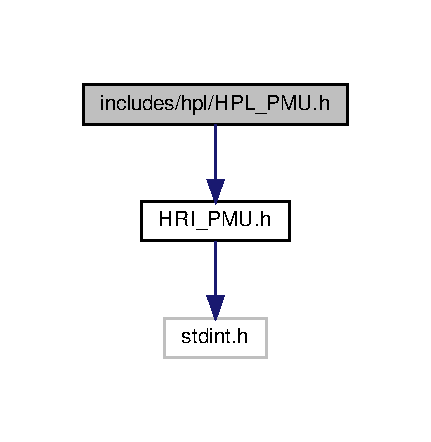
\includegraphics[width=207pt]{HPL__PMU_8h__incl}
\end{center}
\end{figure}
Gráfico de los archivos que directa o indirectamente incluyen a este archivo\+:\nopagebreak
\begin{figure}[H]
\begin{center}
\leavevmode
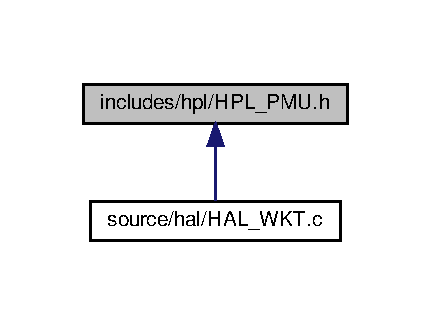
\includegraphics[width=207pt]{HPL__PMU_8h__dep__incl}
\end{center}
\end{figure}
\subsection*{Enumeraciones}
\begin{DoxyCompactItemize}
\item 
\mbox{\Hypertarget{HPL__PMU_8h_a15ae5688f750d988a2ba2d61b089f51d}\label{HPL__PMU_8h_a15ae5688f750d988a2ba2d61b089f51d}} 
enum {\bfseries P\+M\+U\+\_\+sleep\+\_\+mode\+\_\+en} \{ {\bfseries P\+M\+U\+\_\+\+S\+L\+E\+E\+P\+\_\+\+M\+O\+D\+E\+\_\+\+S\+L\+E\+EP} = 0, 
{\bfseries P\+M\+U\+\_\+\+S\+L\+E\+E\+P\+\_\+\+M\+O\+D\+E\+\_\+\+D\+E\+E\+P\+\_\+\+S\+L\+E\+EP}
 \}
\item 
\mbox{\Hypertarget{HPL__PMU_8h_a920560696e0f421c003cab60fa7462e0}\label{HPL__PMU_8h_a920560696e0f421c003cab60fa7462e0}} 
enum {\bfseries P\+M\+U\+\_\+power\+\_\+mode\+\_\+en} \{ {\bfseries P\+M\+U\+\_\+\+P\+O\+W\+E\+R\+\_\+\+M\+O\+D\+E\+\_\+\+D\+E\+F\+A\+U\+LT} = 0, 
{\bfseries P\+M\+U\+\_\+\+P\+O\+W\+E\+R\+\_\+\+M\+O\+D\+E\+\_\+\+D\+E\+E\+P\+\_\+\+S\+L\+E\+EP}, 
{\bfseries P\+M\+U\+\_\+\+P\+O\+W\+E\+R\+\_\+\+M\+O\+D\+E\+\_\+\+P\+O\+W\+E\+R\+\_\+\+D\+O\+WN}, 
{\bfseries P\+M\+U\+\_\+\+P\+O\+W\+E\+R\+\_\+\+M\+O\+D\+E\+\_\+\+D\+E\+E\+P\+\_\+\+P\+O\+W\+E\+R\+\_\+\+D\+O\+WN}
 \}
\item 
\mbox{\Hypertarget{HPL__PMU_8h_a1419270d184f999cd0b1d7fa2d211bd0}\label{HPL__PMU_8h_a1419270d184f999cd0b1d7fa2d211bd0}} 
enum {\bfseries P\+M\+U\+\_\+general\+\_\+purpouse\+\_\+regiter\+\_\+en} \{ {\bfseries P\+M\+U\+\_\+\+G\+E\+N\+E\+R\+A\+L\+\_\+\+P\+U\+R\+P\+O\+U\+S\+E\+\_\+\+R\+E\+G\+I\+S\+T\+E\+R\+\_\+0} = 0, 
{\bfseries P\+M\+U\+\_\+\+G\+E\+N\+E\+R\+A\+L\+\_\+\+P\+U\+R\+P\+O\+U\+S\+E\+\_\+\+R\+E\+G\+I\+S\+T\+E\+R\+\_\+1}, 
{\bfseries P\+M\+U\+\_\+\+G\+E\+N\+E\+R\+A\+L\+\_\+\+P\+U\+R\+P\+O\+U\+S\+E\+\_\+\+R\+E\+G\+I\+S\+T\+E\+R\+\_\+2}, 
{\bfseries P\+M\+U\+\_\+\+G\+E\+N\+E\+R\+A\+L\+\_\+\+P\+U\+R\+P\+O\+U\+S\+E\+\_\+\+R\+E\+G\+I\+S\+T\+E\+R\+\_\+3}
 \}
\end{DoxyCompactItemize}
\subsection*{Funciones}
\begin{DoxyCompactItemize}
\item 
\mbox{\Hypertarget{HPL__PMU_8h_afb6c24248c526f07a9e42cba5688b33c}\label{HPL__PMU_8h_afb6c24248c526f07a9e42cba5688b33c}} 
static void \hyperlink{HPL__PMU_8h_afb6c24248c526f07a9e42cba5688b33c}{P\+M\+U\+\_\+set\+\_\+sleep\+\_\+on\+\_\+exit} (void)
\begin{DoxyCompactList}\small\item\em Activar funcion sleep on exit. \end{DoxyCompactList}\item 
\mbox{\Hypertarget{HPL__PMU_8h_a9e542012e15ef79ba4c4078ecfcd54ac}\label{HPL__PMU_8h_a9e542012e15ef79ba4c4078ecfcd54ac}} 
static void \hyperlink{HPL__PMU_8h_a9e542012e15ef79ba4c4078ecfcd54ac}{P\+M\+U\+\_\+clear\+\_\+sleep\+\_\+on\+\_\+exit} (void)
\begin{DoxyCompactList}\small\item\em Desactivar funcion sleep on exit. \end{DoxyCompactList}\item 
static void \hyperlink{HPL__PMU_8h_a4b8e10e5a96410a9272fa008894c6b39}{P\+M\+U\+\_\+config\+\_\+sleep\+\_\+mode} (P\+M\+U\+\_\+sleep\+\_\+mode\+\_\+en sleep\+\_\+mode)
\begin{DoxyCompactList}\small\item\em Configurar profundidad del sleep. \end{DoxyCompactList}\item 
\mbox{\Hypertarget{HPL__PMU_8h_abbc9c3a999d4388ad883502fa0e37c4d}\label{HPL__PMU_8h_abbc9c3a999d4388ad883502fa0e37c4d}} 
static void {\bfseries P\+M\+U\+\_\+set\+\_\+send\+\_\+event\+\_\+on\+\_\+pending\+\_\+bit} (void)
\item 
\mbox{\Hypertarget{HPL__PMU_8h_a59e5dae637062862b2331212817c0db5}\label{HPL__PMU_8h_a59e5dae637062862b2331212817c0db5}} 
static void {\bfseries P\+M\+U\+\_\+clear\+\_\+send\+\_\+event\+\_\+on\+\_\+pending\+\_\+bit} (void)
\item 
static void \hyperlink{HPL__PMU_8h_a1dbc595b2cec79d958cf4e4334c67497}{P\+M\+U\+\_\+config\+\_\+power\+\_\+mode} (P\+M\+U\+\_\+power\+\_\+mode\+\_\+en power\+\_\+mode)
\begin{DoxyCompactList}\small\item\em Configurar modo de energia en W\+FI. \end{DoxyCompactList}\item 
static void \hyperlink{HPL__PMU_8h_aae2b3dbd3d5a00852beb1b116dfc0e83}{P\+M\+U\+\_\+set\+\_\+prevent\+\_\+deep\+\_\+power} (void)
\begin{DoxyCompactList}\small\item\em Inhabilitar deep power-\/down mode en W\+FI. \end{DoxyCompactList}\item 
\mbox{\Hypertarget{HPL__PMU_8h_a3b4aa57b74bd64bd78ee8a9e43da68f8}\label{HPL__PMU_8h_a3b4aa57b74bd64bd78ee8a9e43da68f8}} 
static uint8\+\_\+t {\bfseries P\+M\+U\+\_\+get\+\_\+sleep\+\_\+flag} (void)
\item 
\mbox{\Hypertarget{HPL__PMU_8h_ab90d308e966e113e088579cf55f20247}\label{HPL__PMU_8h_ab90d308e966e113e088579cf55f20247}} 
static void {\bfseries P\+M\+U\+\_\+clear\+\_\+sleep\+\_\+flag} (void)
\item 
\mbox{\Hypertarget{HPL__PMU_8h_aae5f1c48e584e0bfbfc8cc44d11c1320}\label{HPL__PMU_8h_aae5f1c48e584e0bfbfc8cc44d11c1320}} 
static uint8\+\_\+t {\bfseries P\+M\+U\+\_\+get\+\_\+deep\+\_\+power\+\_\+down\+\_\+flag} (void)
\item 
\mbox{\Hypertarget{HPL__PMU_8h_a208bb9db3ebb7e8f26c467e36162c940}\label{HPL__PMU_8h_a208bb9db3ebb7e8f26c467e36162c940}} 
static void {\bfseries P\+M\+U\+\_\+clear\+\_\+deep\+\_\+power\+\_\+down\+\_\+flag} (void)
\item 
static void \hyperlink{HPL__PMU_8h_a480943821d2cbe85fdb106ee2e8c4293}{P\+M\+U\+\_\+write\+\_\+general\+\_\+purpouse\+\_\+register} (P\+M\+U\+\_\+general\+\_\+purpouse\+\_\+regiter\+\_\+en reg, uint32\+\_\+t data)
\begin{DoxyCompactList}\small\item\em Escibir un dato en un registro de proposito general. \end{DoxyCompactList}\item 
static uint32\+\_\+t \hyperlink{HPL__PMU_8h_a93b9df4c70e7c4e5e4c42196c23f1c03}{P\+M\+U\+\_\+read\+\_\+general\+\_\+purpouse\+\_\+register} (P\+M\+U\+\_\+general\+\_\+purpouse\+\_\+regiter\+\_\+en reg)
\begin{DoxyCompactList}\small\item\em Leer un dato en un registro de proposito general. \end{DoxyCompactList}\item 
\mbox{\Hypertarget{HPL__PMU_8h_ac9fcc7400c44e4761fe568337084dfc7}\label{HPL__PMU_8h_ac9fcc7400c44e4761fe568337084dfc7}} 
static void \hyperlink{HPL__PMU_8h_ac9fcc7400c44e4761fe568337084dfc7}{P\+M\+U\+\_\+enable\+\_\+wake\+\_\+up\+\_\+pin\+\_\+hysteresis} (void)
\begin{DoxyCompactList}\small\item\em Habilitar histeresis en el pin wake up. \end{DoxyCompactList}\item 
\mbox{\Hypertarget{HPL__PMU_8h_aea9d4d56230e7b07395ee9955a7a3289}\label{HPL__PMU_8h_aea9d4d56230e7b07395ee9955a7a3289}} 
static void \hyperlink{HPL__PMU_8h_aea9d4d56230e7b07395ee9955a7a3289}{P\+M\+U\+\_\+disable\+\_\+wake\+\_\+up\+\_\+pin\+\_\+hysteresis} (void)
\begin{DoxyCompactList}\small\item\em Inhabilitar histeresis en el pin wake up. \end{DoxyCompactList}\item 
\mbox{\Hypertarget{HPL__PMU_8h_ab4a1425f0dbbd3248a4734c674736be5}\label{HPL__PMU_8h_ab4a1425f0dbbd3248a4734c674736be5}} 
static void \hyperlink{HPL__PMU_8h_ab4a1425f0dbbd3248a4734c674736be5}{P\+M\+U\+\_\+enable\+\_\+wake\+\_\+up\+\_\+pin} (void)
\begin{DoxyCompactList}\small\item\em Habilitar wake up pin. \end{DoxyCompactList}\item 
\mbox{\Hypertarget{HPL__PMU_8h_aa737bc6c62744375519095f1d1105d0d}\label{HPL__PMU_8h_aa737bc6c62744375519095f1d1105d0d}} 
static void \hyperlink{HPL__PMU_8h_aa737bc6c62744375519095f1d1105d0d}{P\+M\+U\+\_\+disable\+\_\+wake\+\_\+up\+\_\+pin} (void)
\begin{DoxyCompactList}\small\item\em Inhabilitar wake up pin. \end{DoxyCompactList}\item 
\mbox{\Hypertarget{HPL__PMU_8h_a004a16eccd8d515f432ba0b4be928c58}\label{HPL__PMU_8h_a004a16eccd8d515f432ba0b4be928c58}} 
static void \hyperlink{HPL__PMU_8h_a004a16eccd8d515f432ba0b4be928c58}{P\+M\+U\+\_\+enable\+\_\+low\+\_\+power\+\_\+oscillator} (void)
\begin{DoxyCompactList}\small\item\em Habilitar low-\/power oscillator. \end{DoxyCompactList}\item 
\mbox{\Hypertarget{HPL__PMU_8h_a869ad2d3eeeb2dfb6a59a9787edd9b65}\label{HPL__PMU_8h_a869ad2d3eeeb2dfb6a59a9787edd9b65}} 
static void \hyperlink{HPL__PMU_8h_a869ad2d3eeeb2dfb6a59a9787edd9b65}{P\+M\+U\+\_\+disable\+\_\+low\+\_\+power\+\_\+oscillator} (void)
\begin{DoxyCompactList}\small\item\em Inhabilitar low-\/power oscillator. \end{DoxyCompactList}\item 
\mbox{\Hypertarget{HPL__PMU_8h_a1d849e3fbe94001891766f3551c92f7f}\label{HPL__PMU_8h_a1d849e3fbe94001891766f3551c92f7f}} 
static void \hyperlink{HPL__PMU_8h_a1d849e3fbe94001891766f3551c92f7f}{P\+M\+U\+\_\+enable\+\_\+low\+\_\+power\+\_\+oscillator\+\_\+in\+\_\+dpdmode} (void)
\begin{DoxyCompactList}\small\item\em Habilitar low-\/power oscillator en deep power-\/down mode. \end{DoxyCompactList}\item 
\mbox{\Hypertarget{HPL__PMU_8h_a6eaf1acc35f574faa71808a850b3aad1}\label{HPL__PMU_8h_a6eaf1acc35f574faa71808a850b3aad1}} 
static void \hyperlink{HPL__PMU_8h_a6eaf1acc35f574faa71808a850b3aad1}{P\+M\+U\+\_\+disable\+\_\+low\+\_\+power\+\_\+oscillator\+\_\+in\+\_\+dpdmode} (void)
\begin{DoxyCompactList}\small\item\em Inhabilitar low-\/power oscillator en deep power-\/down mode. \end{DoxyCompactList}\item 
\mbox{\Hypertarget{HPL__PMU_8h_aaeff48aa639baa8cad75f3a945a3bffb}\label{HPL__PMU_8h_aaeff48aa639baa8cad75f3a945a3bffb}} 
static void {\bfseries P\+M\+U\+\_\+enable\+\_\+wake\+\_\+up\+\_\+clock\+\_\+hysteresis} (void)
\item 
\mbox{\Hypertarget{HPL__PMU_8h_a2855a9b986a5b3ba62ffcced47174441}\label{HPL__PMU_8h_a2855a9b986a5b3ba62ffcced47174441}} 
static void {\bfseries P\+M\+U\+\_\+disable\+\_\+wake\+\_\+up\+\_\+clock\+\_\+hysteresis} (void)
\item 
\mbox{\Hypertarget{HPL__PMU_8h_abf8e69d642acbc73b9c527beda32652d}\label{HPL__PMU_8h_abf8e69d642acbc73b9c527beda32652d}} 
static void \hyperlink{HPL__PMU_8h_abf8e69d642acbc73b9c527beda32652d}{P\+M\+U\+\_\+enable\+\_\+wake\+\_\+up\+\_\+clock\+\_\+pin} (void)
\begin{DoxyCompactList}\small\item\em Habilitar el pin del clock externo de wake up. \end{DoxyCompactList}\item 
\mbox{\Hypertarget{HPL__PMU_8h_af4e52677186123b4f7d4f0eff504e9b8}\label{HPL__PMU_8h_af4e52677186123b4f7d4f0eff504e9b8}} 
static void \hyperlink{HPL__PMU_8h_af4e52677186123b4f7d4f0eff504e9b8}{P\+M\+U\+\_\+disable\+\_\+wake\+\_\+up\+\_\+clock\+\_\+pin} (void)
\begin{DoxyCompactList}\small\item\em Inhabilitar el pin del clock externo de wake up. \end{DoxyCompactList}\item 
\mbox{\Hypertarget{HPL__PMU_8h_a74ae2254b4e45c193ddcfd7456c9bc60}\label{HPL__PMU_8h_a74ae2254b4e45c193ddcfd7456c9bc60}} 
static void \hyperlink{HPL__PMU_8h_a74ae2254b4e45c193ddcfd7456c9bc60}{P\+M\+U\+\_\+enable\+\_\+reset\+\_\+hysteresis} (void)
\begin{DoxyCompactList}\small\item\em Habilitar histeresis en el pin de reset. \end{DoxyCompactList}\item 
\mbox{\Hypertarget{HPL__PMU_8h_aefda0e320f54ad1afd7af51712be815e}\label{HPL__PMU_8h_aefda0e320f54ad1afd7af51712be815e}} 
static void \hyperlink{HPL__PMU_8h_aefda0e320f54ad1afd7af51712be815e}{P\+M\+U\+\_\+disable\+\_\+reset\+\_\+hysteresis} (void)
\begin{DoxyCompactList}\small\item\em Inhabilitar histeresis en el pin de reset. \end{DoxyCompactList}\item 
\mbox{\Hypertarget{HPL__PMU_8h_afea5aea4989e597909c677473852c7b0}\label{HPL__PMU_8h_afea5aea4989e597909c677473852c7b0}} 
static void \hyperlink{HPL__PMU_8h_afea5aea4989e597909c677473852c7b0}{P\+M\+U\+\_\+enable\+\_\+reset} (void)
\begin{DoxyCompactList}\small\item\em Habilitar funcion de reset en el pin. \end{DoxyCompactList}\item 
\mbox{\Hypertarget{HPL__PMU_8h_ab151df29424041da414311340cb9609a}\label{HPL__PMU_8h_ab151df29424041da414311340cb9609a}} 
static void \hyperlink{HPL__PMU_8h_ab151df29424041da414311340cb9609a}{P\+M\+U\+\_\+disable\+\_\+reset} (void)
\begin{DoxyCompactList}\small\item\em Inhabilitar funcion de reset en el pin. \end{DoxyCompactList}\end{DoxyCompactItemize}
\subsection*{Variables}
\begin{DoxyCompactItemize}
\item 
\mbox{\Hypertarget{HPL__PMU_8h_a200799a46d8cbf9d335ba1358f9527ff}\label{HPL__PMU_8h_a200799a46d8cbf9d335ba1358f9527ff}} 
volatile \hyperlink{HRI__PMU_8h_structSCR__reg__t}{S\+C\+R\+\_\+reg\+\_\+t} $\ast$const \hyperlink{HPL__PMU_8h_a200799a46d8cbf9d335ba1358f9527ff}{S\+CR}
\begin{DoxyCompactList}\small\item\em Registro S\+CR. \end{DoxyCompactList}\item 
\mbox{\Hypertarget{HPL__PMU_8h_aa836cf8f31c591ca7035c321cfdfaa93}\label{HPL__PMU_8h_aa836cf8f31c591ca7035c321cfdfaa93}} 
volatile \hyperlink{HRI__PMU_8h_structPMU__per__t}{P\+M\+U\+\_\+per\+\_\+t} $\ast$const \hyperlink{HPL__PMU_8h_aa836cf8f31c591ca7035c321cfdfaa93}{P\+MU}
\begin{DoxyCompactList}\small\item\em Periferico P\+MU. \end{DoxyCompactList}\end{DoxyCompactItemize}


\subsection{Descripción detallada}
Declaraciones a nivel de abstraccion de periferico del P\+MU (L\+P\+C845) 

\begin{DoxyAuthor}{Autor}
Augusto Santini 
\end{DoxyAuthor}
\begin{DoxyDate}{Fecha}
4/2020 
\end{DoxyDate}
\begin{DoxyVersion}{Versión}
1.\+0 
\end{DoxyVersion}


\subsection{Documentación de las funciones}
\mbox{\Hypertarget{HPL__PMU_8h_a4b8e10e5a96410a9272fa008894c6b39}\label{HPL__PMU_8h_a4b8e10e5a96410a9272fa008894c6b39}} 
\index{H\+P\+L\+\_\+\+P\+M\+U.\+h@{H\+P\+L\+\_\+\+P\+M\+U.\+h}!P\+M\+U\+\_\+config\+\_\+sleep\+\_\+mode@{P\+M\+U\+\_\+config\+\_\+sleep\+\_\+mode}}
\index{P\+M\+U\+\_\+config\+\_\+sleep\+\_\+mode@{P\+M\+U\+\_\+config\+\_\+sleep\+\_\+mode}!H\+P\+L\+\_\+\+P\+M\+U.\+h@{H\+P\+L\+\_\+\+P\+M\+U.\+h}}
\subsubsection{\texorpdfstring{P\+M\+U\+\_\+config\+\_\+sleep\+\_\+mode()}{PMU\_config\_sleep\_mode()}}
{\footnotesize\ttfamily static void P\+M\+U\+\_\+config\+\_\+sleep\+\_\+mode (\begin{DoxyParamCaption}\item[{P\+M\+U\+\_\+sleep\+\_\+mode\+\_\+en}]{sleep\+\_\+mode }\end{DoxyParamCaption})\hspace{0.3cm}{\ttfamily [inline]}, {\ttfamily [static]}}



Configurar profundidad del sleep. 


\begin{DoxyParams}[1]{Parámetros}
\mbox{\tt in}  & {\em sleep\+\_\+mode} & Profundidad del sleep deseada \\
\hline
\end{DoxyParams}
\mbox{\Hypertarget{HPL__PMU_8h_a1dbc595b2cec79d958cf4e4334c67497}\label{HPL__PMU_8h_a1dbc595b2cec79d958cf4e4334c67497}} 
\index{H\+P\+L\+\_\+\+P\+M\+U.\+h@{H\+P\+L\+\_\+\+P\+M\+U.\+h}!P\+M\+U\+\_\+config\+\_\+power\+\_\+mode@{P\+M\+U\+\_\+config\+\_\+power\+\_\+mode}}
\index{P\+M\+U\+\_\+config\+\_\+power\+\_\+mode@{P\+M\+U\+\_\+config\+\_\+power\+\_\+mode}!H\+P\+L\+\_\+\+P\+M\+U.\+h@{H\+P\+L\+\_\+\+P\+M\+U.\+h}}
\subsubsection{\texorpdfstring{P\+M\+U\+\_\+config\+\_\+power\+\_\+mode()}{PMU\_config\_power\_mode()}}
{\footnotesize\ttfamily static void P\+M\+U\+\_\+config\+\_\+power\+\_\+mode (\begin{DoxyParamCaption}\item[{P\+M\+U\+\_\+power\+\_\+mode\+\_\+en}]{power\+\_\+mode }\end{DoxyParamCaption})\hspace{0.3cm}{\ttfamily [inline]}, {\ttfamily [static]}}



Configurar modo de energia en W\+FI. 


\begin{DoxyParams}[1]{Parámetros}
\mbox{\tt in}  & {\em power\+\_\+mode} & Modo de energia deseado \\
\hline
\end{DoxyParams}
\mbox{\Hypertarget{HPL__PMU_8h_aae2b3dbd3d5a00852beb1b116dfc0e83}\label{HPL__PMU_8h_aae2b3dbd3d5a00852beb1b116dfc0e83}} 
\index{H\+P\+L\+\_\+\+P\+M\+U.\+h@{H\+P\+L\+\_\+\+P\+M\+U.\+h}!P\+M\+U\+\_\+set\+\_\+prevent\+\_\+deep\+\_\+power@{P\+M\+U\+\_\+set\+\_\+prevent\+\_\+deep\+\_\+power}}
\index{P\+M\+U\+\_\+set\+\_\+prevent\+\_\+deep\+\_\+power@{P\+M\+U\+\_\+set\+\_\+prevent\+\_\+deep\+\_\+power}!H\+P\+L\+\_\+\+P\+M\+U.\+h@{H\+P\+L\+\_\+\+P\+M\+U.\+h}}
\subsubsection{\texorpdfstring{P\+M\+U\+\_\+set\+\_\+prevent\+\_\+deep\+\_\+power()}{PMU\_set\_prevent\_deep\_power()}}
{\footnotesize\ttfamily static void P\+M\+U\+\_\+set\+\_\+prevent\+\_\+deep\+\_\+power (\begin{DoxyParamCaption}\item[{void}]{ }\end{DoxyParamCaption})\hspace{0.3cm}{\ttfamily [inline]}, {\ttfamily [static]}}



Inhabilitar deep power-\/down mode en W\+FI. 

Inhabilita el deep power-\/down mode, aunque este configurado en ese modo, hasta el proximo reset \mbox{\Hypertarget{HPL__PMU_8h_a480943821d2cbe85fdb106ee2e8c4293}\label{HPL__PMU_8h_a480943821d2cbe85fdb106ee2e8c4293}} 
\index{H\+P\+L\+\_\+\+P\+M\+U.\+h@{H\+P\+L\+\_\+\+P\+M\+U.\+h}!P\+M\+U\+\_\+write\+\_\+general\+\_\+purpouse\+\_\+register@{P\+M\+U\+\_\+write\+\_\+general\+\_\+purpouse\+\_\+register}}
\index{P\+M\+U\+\_\+write\+\_\+general\+\_\+purpouse\+\_\+register@{P\+M\+U\+\_\+write\+\_\+general\+\_\+purpouse\+\_\+register}!H\+P\+L\+\_\+\+P\+M\+U.\+h@{H\+P\+L\+\_\+\+P\+M\+U.\+h}}
\subsubsection{\texorpdfstring{P\+M\+U\+\_\+write\+\_\+general\+\_\+purpouse\+\_\+register()}{PMU\_write\_general\_purpouse\_register()}}
{\footnotesize\ttfamily static void P\+M\+U\+\_\+write\+\_\+general\+\_\+purpouse\+\_\+register (\begin{DoxyParamCaption}\item[{P\+M\+U\+\_\+general\+\_\+purpouse\+\_\+regiter\+\_\+en}]{reg,  }\item[{uint32\+\_\+t}]{data }\end{DoxyParamCaption})\hspace{0.3cm}{\ttfamily [inline]}, {\ttfamily [static]}}



Escibir un dato en un registro de proposito general. 


\begin{DoxyParams}[1]{Parámetros}
\mbox{\tt in}  & {\em reg} & Numero de registro a escribir \\
\hline
\mbox{\tt in}  & {\em data} & Dato a escribir en el registro de proposito general \\
\hline
\end{DoxyParams}
\mbox{\Hypertarget{HPL__PMU_8h_a93b9df4c70e7c4e5e4c42196c23f1c03}\label{HPL__PMU_8h_a93b9df4c70e7c4e5e4c42196c23f1c03}} 
\index{H\+P\+L\+\_\+\+P\+M\+U.\+h@{H\+P\+L\+\_\+\+P\+M\+U.\+h}!P\+M\+U\+\_\+read\+\_\+general\+\_\+purpouse\+\_\+register@{P\+M\+U\+\_\+read\+\_\+general\+\_\+purpouse\+\_\+register}}
\index{P\+M\+U\+\_\+read\+\_\+general\+\_\+purpouse\+\_\+register@{P\+M\+U\+\_\+read\+\_\+general\+\_\+purpouse\+\_\+register}!H\+P\+L\+\_\+\+P\+M\+U.\+h@{H\+P\+L\+\_\+\+P\+M\+U.\+h}}
\subsubsection{\texorpdfstring{P\+M\+U\+\_\+read\+\_\+general\+\_\+purpouse\+\_\+register()}{PMU\_read\_general\_purpouse\_register()}}
{\footnotesize\ttfamily static uint32\+\_\+t P\+M\+U\+\_\+read\+\_\+general\+\_\+purpouse\+\_\+register (\begin{DoxyParamCaption}\item[{P\+M\+U\+\_\+general\+\_\+purpouse\+\_\+regiter\+\_\+en}]{reg }\end{DoxyParamCaption})\hspace{0.3cm}{\ttfamily [inline]}, {\ttfamily [static]}}



Leer un dato en un registro de proposito general. 


\begin{DoxyParams}[1]{Parámetros}
\mbox{\tt in}  & {\em reg} & Numero de registro a escribir \\
\hline
\end{DoxyParams}
\begin{DoxyReturn}{Devuelve}
Dato en el registro de proposito general 
\end{DoxyReturn}

\hypertarget{HPL__SPI_8h}{}\section{Referencia del Archivo includes/hpl/\+H\+P\+L\+\_\+\+S\+PI.h}
\label{HPL__SPI_8h}\index{includes/hpl/\+H\+P\+L\+\_\+\+S\+P\+I.\+h@{includes/hpl/\+H\+P\+L\+\_\+\+S\+P\+I.\+h}}


Declaraciones a nivel de abstraccion de periferico del S\+PI (L\+P\+C845)  


{\ttfamily \#include $<$H\+R\+I\+\_\+\+S\+P\+I.\+h$>$}\newline
Dependencia gráfica adjunta para H\+P\+L\+\_\+\+S\+P\+I.\+h\+:\nopagebreak
\begin{figure}[H]
\begin{center}
\leavevmode
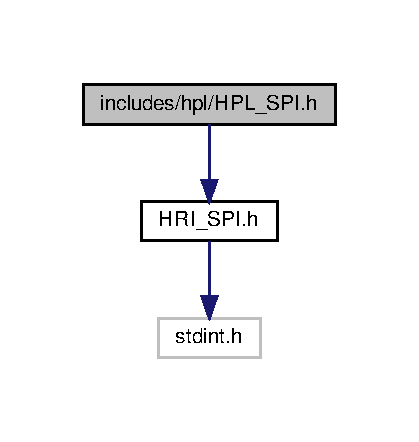
\includegraphics[width=201pt]{HPL__SPI_8h__incl}
\end{center}
\end{figure}
Gráfico de los archivos que directa o indirectamente incluyen a este archivo\+:\nopagebreak
\begin{figure}[H]
\begin{center}
\leavevmode
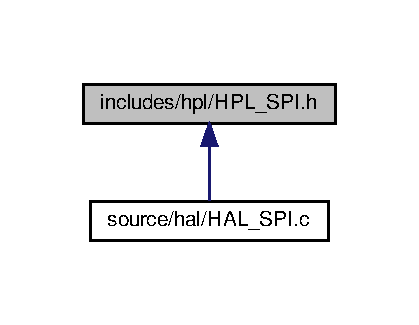
\includegraphics[width=201pt]{HPL__SPI_8h__dep__incl}
\end{center}
\end{figure}
\subsection*{Enumeraciones}
\begin{DoxyCompactItemize}
\item 
\mbox{\Hypertarget{HPL__SPI_8h_a66672558a7fdeaca7b39014413f3336b}\label{HPL__SPI_8h_a66672558a7fdeaca7b39014413f3336b}} 
enum {\bfseries S\+P\+I\+\_\+status\+\_\+flag\+\_\+en} \{ \newline
{\bfseries S\+P\+I\+\_\+\+S\+T\+A\+T\+U\+S\+\_\+\+F\+L\+A\+G\+\_\+\+R\+X\+R\+DY} = 0, 
{\bfseries S\+P\+I\+\_\+\+S\+T\+A\+T\+U\+S\+\_\+\+F\+L\+A\+G\+\_\+\+T\+X\+R\+DY}, 
{\bfseries S\+P\+I\+\_\+\+S\+T\+A\+T\+U\+S\+\_\+\+F\+L\+A\+G\+\_\+\+R\+X\+OV}, 
{\bfseries S\+P\+I\+\_\+\+S\+T\+A\+T\+U\+S\+\_\+\+F\+L\+A\+G\+\_\+\+T\+X\+UR}, 
\newline
{\bfseries S\+P\+I\+\_\+\+S\+T\+A\+T\+U\+S\+\_\+\+F\+L\+A\+G\+\_\+\+S\+SA}, 
{\bfseries S\+P\+I\+\_\+\+S\+T\+A\+T\+U\+S\+\_\+\+F\+L\+A\+G\+\_\+\+S\+SD}, 
{\bfseries S\+P\+I\+\_\+\+S\+T\+A\+T\+U\+S\+\_\+\+F\+L\+A\+G\+\_\+\+S\+T\+A\+L\+L\+ED}, 
{\bfseries S\+P\+I\+\_\+\+S\+T\+A\+T\+U\+S\+\_\+\+F\+L\+A\+G\+\_\+\+E\+N\+D\+T\+R\+A\+N\+S\+F\+ER}, 
\newline
{\bfseries S\+P\+I\+\_\+\+S\+T\+A\+T\+U\+S\+\_\+\+F\+L\+A\+G\+\_\+\+M\+S\+T\+I\+D\+LE}
 \}
\item 
\mbox{\Hypertarget{HPL__SPI_8h_af1f18c9818dad3ea393e5d22da90eccb}\label{HPL__SPI_8h_af1f18c9818dad3ea393e5d22da90eccb}} 
enum {\bfseries S\+P\+I\+\_\+irq\+\_\+sel\+\_\+en} \{ \newline
{\bfseries S\+P\+I\+\_\+\+I\+R\+Q\+\_\+\+R\+X\+R\+DY} = 0, 
{\bfseries S\+P\+I\+\_\+\+I\+R\+Q\+\_\+\+T\+X\+R\+DY}, 
{\bfseries S\+P\+I\+\_\+\+I\+R\+Q\+\_\+\+R\+X\+OV}, 
{\bfseries S\+P\+I\+\_\+\+I\+R\+Q\+\_\+\+T\+X\+UR}, 
\newline
{\bfseries S\+P\+I\+\_\+\+I\+R\+Q\+\_\+\+S\+SA}, 
{\bfseries S\+P\+I\+\_\+\+I\+R\+Q\+\_\+\+S\+SD}
 \}
\item 
\mbox{\Hypertarget{HPL__SPI_8h_ae9e7128defe4b247e76fd82088c6539d}\label{HPL__SPI_8h_ae9e7128defe4b247e76fd82088c6539d}} 
enum {\bfseries S\+P\+I\+\_\+data\+\_\+length\+\_\+en} \{ \newline
{\bfseries S\+P\+I\+\_\+\+D\+A\+T\+A\+\_\+\+L\+E\+N\+G\+T\+H\+\_\+1\+\_\+\+B\+IT} = 0, 
{\bfseries S\+P\+I\+\_\+\+D\+A\+T\+A\+\_\+\+L\+E\+N\+G\+T\+H\+\_\+2\+\_\+\+B\+IT}, 
{\bfseries S\+P\+I\+\_\+\+D\+A\+T\+A\+\_\+\+L\+E\+N\+G\+T\+H\+\_\+3\+\_\+\+B\+IT}, 
{\bfseries S\+P\+I\+\_\+\+D\+A\+T\+A\+\_\+\+L\+E\+N\+G\+T\+H\+\_\+4\+\_\+\+B\+IT}, 
\newline
{\bfseries S\+P\+I\+\_\+\+D\+A\+T\+A\+\_\+\+L\+E\+N\+G\+T\+H\+\_\+5\+\_\+\+B\+IT}, 
{\bfseries S\+P\+I\+\_\+\+D\+A\+T\+A\+\_\+\+L\+E\+N\+G\+T\+H\+\_\+6\+\_\+\+B\+IT}, 
{\bfseries S\+P\+I\+\_\+\+D\+A\+T\+A\+\_\+\+L\+E\+N\+G\+T\+H\+\_\+7\+\_\+\+B\+IT}, 
{\bfseries S\+P\+I\+\_\+\+D\+A\+T\+A\+\_\+\+L\+E\+N\+G\+T\+H\+\_\+8\+\_\+\+B\+IT}, 
\newline
{\bfseries S\+P\+I\+\_\+\+D\+A\+T\+A\+\_\+\+L\+E\+N\+G\+T\+H\+\_\+9\+\_\+\+B\+IT}, 
{\bfseries S\+P\+I\+\_\+\+D\+A\+T\+A\+\_\+\+L\+E\+N\+G\+T\+H\+\_\+10\+\_\+\+B\+IT}, 
{\bfseries S\+P\+I\+\_\+\+D\+A\+T\+A\+\_\+\+L\+E\+N\+G\+T\+H\+\_\+11\+\_\+\+B\+IT}, 
{\bfseries S\+P\+I\+\_\+\+D\+A\+T\+A\+\_\+\+L\+E\+N\+G\+T\+H\+\_\+12\+\_\+\+B\+IT}, 
\newline
{\bfseries S\+P\+I\+\_\+\+D\+A\+T\+A\+\_\+\+L\+E\+N\+G\+T\+H\+\_\+13\+\_\+\+B\+IT}, 
{\bfseries S\+P\+I\+\_\+\+D\+A\+T\+A\+\_\+\+L\+E\+N\+G\+T\+H\+\_\+14\+\_\+\+B\+IT}, 
{\bfseries S\+P\+I\+\_\+\+D\+A\+T\+A\+\_\+\+L\+E\+N\+G\+T\+H\+\_\+15\+\_\+\+B\+IT}, 
{\bfseries S\+P\+I\+\_\+\+D\+A\+T\+A\+\_\+\+L\+E\+N\+G\+T\+H\+\_\+16\+\_\+\+B\+IT}
 \}
\end{DoxyCompactItemize}
\subsection*{Funciones}
\begin{DoxyCompactItemize}
\item 
static void \hyperlink{HPL__SPI_8h_a7f5a0bc037eb9b128ea506e7222bbd73}{S\+P\+I\+\_\+enable} (uint8\+\_\+t inst)
\begin{DoxyCompactList}\small\item\em Habilitar modulo. \end{DoxyCompactList}\item 
static void \hyperlink{HPL__SPI_8h_ab1bba7aff2d296ddafe2c9b45fe4d87c}{S\+P\+I\+\_\+disable} (uint8\+\_\+t inst)
\begin{DoxyCompactList}\small\item\em Inhabilitar modulo. \end{DoxyCompactList}\item 
static void \hyperlink{HPL__SPI_8h_af78e337a45a4c2e136f7120342076d28}{S\+P\+I\+\_\+set\+\_\+master\+\_\+mode} (uint8\+\_\+t inst)
\begin{DoxyCompactList}\small\item\em Configurar como modo master. \end{DoxyCompactList}\item 
static void \hyperlink{HPL__SPI_8h_a83a643a96e2d7e2fdc6615cc15bd594f}{S\+P\+I\+\_\+set\+\_\+slave\+\_\+mode} (uint8\+\_\+t inst)
\begin{DoxyCompactList}\small\item\em Configurar como modo slave. \end{DoxyCompactList}\item 
static void \hyperlink{HPL__SPI_8h_a35b37109680a1a90b58761fc50c60bcc}{S\+P\+I\+\_\+set\+\_\+data\+\_\+order\+\_\+msb\+\_\+first} (uint8\+\_\+t inst)
\begin{DoxyCompactList}\small\item\em Configurar orden de datos M\+SB primero. \end{DoxyCompactList}\item 
static void \hyperlink{HPL__SPI_8h_a98dc4ab9ac329763002b24ad1f8430de}{S\+P\+I\+\_\+set\+\_\+data\+\_\+order\+\_\+lsb\+\_\+first} (uint8\+\_\+t inst)
\begin{DoxyCompactList}\small\item\em Configurar orden de datos L\+SB primero. \end{DoxyCompactList}\item 
static void \hyperlink{HPL__SPI_8h_a0f4df7d4b8e939e46377d8468b45aad1}{S\+P\+I\+\_\+set\+\_\+cpha\+\_\+change} (uint8\+\_\+t inst)
\begin{DoxyCompactList}\small\item\em Configurar fase del clock (modo change) \end{DoxyCompactList}\item 
static void \hyperlink{HPL__SPI_8h_aa353bf9381d4d1039eb57e91df994b17}{S\+P\+I\+\_\+set\+\_\+cpha\+\_\+capture} (uint8\+\_\+t inst)
\begin{DoxyCompactList}\small\item\em Configurar fase del clock (modo capture) \end{DoxyCompactList}\item 
static void \hyperlink{HPL__SPI_8h_a4fddd1f3564674ba202af7449edfbf74}{S\+P\+I\+\_\+set\+\_\+cpol\+\_\+low} (uint8\+\_\+t inst)
\begin{DoxyCompactList}\small\item\em Configurar polaridad del clock (polaridad baja) \end{DoxyCompactList}\item 
static void \hyperlink{HPL__SPI_8h_a111a8fc439e9c8a4fb4c3526022e43eb}{S\+P\+I\+\_\+set\+\_\+cpol\+\_\+high} (uint8\+\_\+t inst)
\begin{DoxyCompactList}\small\item\em Configurar polaridad del clock (polaridad alta) \end{DoxyCompactList}\item 
static void \hyperlink{HPL__SPI_8h_ace30151bd22a9af188f5c244c84173f9}{S\+P\+I\+\_\+enable\+\_\+loopback\+\_\+mode} (uint8\+\_\+t inst)
\begin{DoxyCompactList}\small\item\em Habilitar modo loopback. \end{DoxyCompactList}\item 
static void \hyperlink{HPL__SPI_8h_a2ad831cb1a119f298131a5a2610482bf}{S\+P\+I\+\_\+disable\+\_\+loopback\+\_\+mode} (uint8\+\_\+t inst)
\begin{DoxyCompactList}\small\item\em Inhabilitar modo loopback. \end{DoxyCompactList}\item 
static void \hyperlink{HPL__SPI_8h_a842e279cf5a2c92b433e5a9ecf5b36a0}{S\+P\+I\+\_\+set\+\_\+ssel\+\_\+active\+\_\+low} (uint8\+\_\+t inst, uint8\+\_\+t channel)
\begin{DoxyCompactList}\small\item\em Fijar polaridad de slave select como activa baja. \end{DoxyCompactList}\item 
static void \hyperlink{HPL__SPI_8h_a29e66c2b2d4a01fc1a1840073a072d0c}{S\+P\+I\+\_\+set\+\_\+ssel\+\_\+active\+\_\+high} (uint8\+\_\+t inst, uint8\+\_\+t channel)
\begin{DoxyCompactList}\small\item\em Fijar polaridad de slave select como activa alta. \end{DoxyCompactList}\item 
static void \hyperlink{HPL__SPI_8h_acff554a0ddf87eaf7eb41b6b56c1e31c}{S\+P\+I\+\_\+set\+\_\+pre\+\_\+delay} (uint8\+\_\+t inst, uint8\+\_\+t delay)
\begin{DoxyCompactList}\small\item\em Configurar ciclos de clock entre la activacion de S\+S\+EL y la transmision de datos. \end{DoxyCompactList}\item 
static void \hyperlink{HPL__SPI_8h_a1a2bf6e750b14df36d98b9fb9d0a2871}{S\+P\+I\+\_\+set\+\_\+post\+\_\+delay} (uint8\+\_\+t inst, uint8\+\_\+t delay)
\begin{DoxyCompactList}\small\item\em Configurar ciclos de clock entre la finalizacion de transmision y desactivacion de S\+S\+EL. \end{DoxyCompactList}\item 
static void \hyperlink{HPL__SPI_8h_a55e94418d222765a9c93cc608f6e2b2e}{S\+P\+I\+\_\+set\+\_\+frame\+\_\+delay} (uint8\+\_\+t inst, uint8\+\_\+t delay)
\begin{DoxyCompactList}\small\item\em Configurar ciclos de clock entre transmisiones sin desactivar S\+S\+EL. \end{DoxyCompactList}\item 
static void \hyperlink{HPL__SPI_8h_ac1a540ea9fa3a69d6d4c6532bbf4eae0}{S\+P\+I\+\_\+set\+\_\+transfer\+\_\+delay} (uint8\+\_\+t inst, uint8\+\_\+t delay)
\begin{DoxyCompactList}\small\item\em Configurar ciclos de clock entre desactivacion/activacion de S\+S\+EL. \end{DoxyCompactList}\item 
static uint8\+\_\+t \hyperlink{HPL__SPI_8h_a6fc886924b3aba2a73125159622ef7f6}{S\+P\+I\+\_\+get\+\_\+status\+\_\+flag} (uint8\+\_\+t inst, S\+P\+I\+\_\+status\+\_\+flag\+\_\+en flag)
\begin{DoxyCompactList}\small\item\em Leer un flag de status. \end{DoxyCompactList}\item 
static uint8\+\_\+t \hyperlink{HPL__SPI_8h_a2e46cfd33feb6983d174ea06d77e4bd6}{S\+P\+I\+\_\+clear\+\_\+status\+\_\+flag} (uint8\+\_\+t inst, S\+P\+I\+\_\+status\+\_\+flag\+\_\+en flag)
\begin{DoxyCompactList}\small\item\em Limpiar un flag de status. \end{DoxyCompactList}\item 
static uint8\+\_\+t \hyperlink{HPL__SPI_8h_ab1549d69ab3371e0f858870e54c3979d}{S\+P\+I\+\_\+enable\+\_\+irq} (uint8\+\_\+t inst, S\+P\+I\+\_\+irq\+\_\+sel\+\_\+en irq)
\begin{DoxyCompactList}\small\item\em Habilitar interrupcion. \end{DoxyCompactList}\item 
static uint8\+\_\+t \hyperlink{HPL__SPI_8h_a81b627aa7a6b4263b1ea33ef489ed3d2}{S\+P\+I\+\_\+disable\+\_\+irq} (uint8\+\_\+t inst, S\+P\+I\+\_\+irq\+\_\+sel\+\_\+en irq)
\begin{DoxyCompactList}\small\item\em Inhabilitar interrupcion. \end{DoxyCompactList}\item 
static uint16\+\_\+t \hyperlink{HPL__SPI_8h_ae937b6836b4517b2b7f3612913412030}{S\+P\+I\+\_\+read\+\_\+rx\+\_\+data} (uint8\+\_\+t inst)
\begin{DoxyCompactList}\small\item\em Leer resultado de la recepcion. \end{DoxyCompactList}\item 
static uint8\+\_\+t \hyperlink{HPL__SPI_8h_a7969888a438cb40a69ae45e23858fca4}{S\+P\+I\+\_\+get\+\_\+active\+\_\+ssl} (uint8\+\_\+t inst)
\begin{DoxyCompactList}\small\item\em Obtener slave select activo. \end{DoxyCompactList}\item 
static uint8\+\_\+t \hyperlink{HPL__SPI_8h_a8a6942ae0d12c3828764b842353e7462}{S\+P\+I\+\_\+get\+\_\+sot\+\_\+flag} (uint8\+\_\+t inst)
\begin{DoxyCompactList}\small\item\em Obtener estado del flag de start of transfer. \end{DoxyCompactList}\item 
static void \hyperlink{HPL__SPI_8h_a5fcb038406b422dcc3c725c1c75d2cd9}{S\+P\+I\+\_\+write\+\_\+txdata} (uint8\+\_\+t inst, uint16\+\_\+t data)
\begin{DoxyCompactList}\small\item\em Escribir registro de datos de transmision. \end{DoxyCompactList}\item 
static void \hyperlink{HPL__SPI_8h_a8c993be947e658cf703bac770be82c9d}{S\+P\+I\+\_\+select\+\_\+slave} (uint8\+\_\+t inst, uint8\+\_\+t channel)
\begin{DoxyCompactList}\small\item\em Habilitar slave select para la proxima transmision. \end{DoxyCompactList}\item 
static void \hyperlink{HPL__SPI_8h_a589229cde66e898378aa1ff4232bba88}{S\+P\+I\+\_\+set\+\_\+end\+\_\+of\+\_\+transmission} (uint8\+\_\+t inst)
\begin{DoxyCompactList}\small\item\em Indicar fin de transmision en la proxima transmision. \end{DoxyCompactList}\item 
static void \hyperlink{HPL__SPI_8h_ad4be5d6c6f7b2d0bef4bb779aeca4658}{S\+P\+I\+\_\+clear\+\_\+end\+\_\+of\+\_\+transmission} (uint8\+\_\+t inst)
\begin{DoxyCompactList}\small\item\em Limpiar fin de transmision en la proxima transmision. \end{DoxyCompactList}\item 
static void \hyperlink{HPL__SPI_8h_a428630c9a5861df7bbf4f48a118ae85b}{S\+P\+I\+\_\+set\+\_\+end\+\_\+of\+\_\+frame} (uint8\+\_\+t inst)
\begin{DoxyCompactList}\small\item\em Indicar fin de trama en la proxima transmision. \end{DoxyCompactList}\item 
static void \hyperlink{HPL__SPI_8h_a5ac9cf28068ff5efff5cd0d0f118d842}{S\+P\+I\+\_\+clear\+\_\+end\+\_\+of\+\_\+frame} (uint8\+\_\+t inst)
\begin{DoxyCompactList}\small\item\em Limpiar fin de trama en la proxima transmision. \end{DoxyCompactList}\item 
static void \hyperlink{HPL__SPI_8h_ae7d463bf945b98eb728350a82317edcc}{S\+P\+I\+\_\+set\+\_\+rx\+\_\+ignore} (uint8\+\_\+t inst)
\begin{DoxyCompactList}\small\item\em Ignorar recepcion en la proxima transmision. \end{DoxyCompactList}\item 
static void \hyperlink{HPL__SPI_8h_a760e2d2006757580d486d2c51462077e}{S\+P\+I\+\_\+clear\+\_\+rx\+\_\+ignore} (uint8\+\_\+t inst)
\begin{DoxyCompactList}\small\item\em No ignorar recepcino en la proxima transmision. \end{DoxyCompactList}\item 
static void \hyperlink{HPL__SPI_8h_a943b0094c742d4c491ffce075d8dce59}{S\+P\+I\+\_\+set\+\_\+data\+\_\+length} (uint8\+\_\+t inst, S\+P\+I\+\_\+data\+\_\+length\+\_\+en data\+\_\+length)
\begin{DoxyCompactList}\small\item\em Configurar largo de bits de palabra. \end{DoxyCompactList}\item 
static void \hyperlink{HPL__SPI_8h_a0622d0a1000a43e328e6abf227bfa7e8}{S\+P\+I\+\_\+set\+\_\+data\+\_\+and\+\_\+control} (uint8\+\_\+t inst, \hyperlink{HRI__SPI_8h_structSPI__TXDATCTL__reg__t}{S\+P\+I\+\_\+\+T\+X\+D\+A\+T\+C\+T\+L\+\_\+reg\+\_\+t} $\ast$data\+\_\+and\+\_\+control)
\begin{DoxyCompactList}\small\item\em Escribir data a transmitir y control al mismo tiempo (en una unica escritura) \end{DoxyCompactList}\item 
static void \hyperlink{HPL__SPI_8h_a8c444a7990eb7b158ea2bdeb4172e37f}{S\+P\+I\+\_\+set\+\_\+clock\+\_\+div} (uint8\+\_\+t inst, uint16\+\_\+t div)
\begin{DoxyCompactList}\small\item\em Configurar divisor de clock. \end{DoxyCompactList}\item 
static uint8\+\_\+t \hyperlink{HPL__SPI_8h_ab580bc0f38853eb701ffd155d0aef866}{S\+P\+I\+\_\+get\+\_\+irq\+\_\+flag\+\_\+status} (uint8\+\_\+t inst, S\+P\+I\+\_\+irq\+\_\+sel\+\_\+en irq)
\begin{DoxyCompactList}\small\item\em Leer flag de interrupcion actual. \end{DoxyCompactList}\end{DoxyCompactItemize}
\subsection*{Variables}
\begin{DoxyCompactItemize}
\item 
\mbox{\Hypertarget{HPL__SPI_8h_a673a4443bf72e54d92cf52e25a1bad65}\label{HPL__SPI_8h_a673a4443bf72e54d92cf52e25a1bad65}} 
volatile \hyperlink{HRI__SPI_8h_structSPI__per__t}{S\+P\+I\+\_\+per\+\_\+t} $\ast$const \hyperlink{HPL__SPI_8h_a673a4443bf72e54d92cf52e25a1bad65}{S\+PI} \mbox{[}$\,$\mbox{]}
\begin{DoxyCompactList}\small\item\em Perifericos S\+PI. \end{DoxyCompactList}\end{DoxyCompactItemize}


\subsection{Descripción detallada}
Declaraciones a nivel de abstraccion de periferico del S\+PI (L\+P\+C845) 

\begin{DoxyAuthor}{Autor}
Augusto Santini 
\end{DoxyAuthor}
\begin{DoxyDate}{Fecha}
3/2020 
\end{DoxyDate}
\begin{DoxyVersion}{Versión}
1.\+0 
\end{DoxyVersion}


\subsection{Documentación de las funciones}
\mbox{\Hypertarget{HPL__SPI_8h_a7f5a0bc037eb9b128ea506e7222bbd73}\label{HPL__SPI_8h_a7f5a0bc037eb9b128ea506e7222bbd73}} 
\index{H\+P\+L\+\_\+\+S\+P\+I.\+h@{H\+P\+L\+\_\+\+S\+P\+I.\+h}!S\+P\+I\+\_\+enable@{S\+P\+I\+\_\+enable}}
\index{S\+P\+I\+\_\+enable@{S\+P\+I\+\_\+enable}!H\+P\+L\+\_\+\+S\+P\+I.\+h@{H\+P\+L\+\_\+\+S\+P\+I.\+h}}
\subsubsection{\texorpdfstring{S\+P\+I\+\_\+enable()}{SPI\_enable()}}
{\footnotesize\ttfamily static void S\+P\+I\+\_\+enable (\begin{DoxyParamCaption}\item[{uint8\+\_\+t}]{inst }\end{DoxyParamCaption})\hspace{0.3cm}{\ttfamily [inline]}, {\ttfamily [static]}}



Habilitar modulo. 


\begin{DoxyParams}[1]{Parámetros}
\mbox{\tt in}  & {\em inst} & Instancia a habilitar \\
\hline
\end{DoxyParams}
\mbox{\Hypertarget{HPL__SPI_8h_ab1bba7aff2d296ddafe2c9b45fe4d87c}\label{HPL__SPI_8h_ab1bba7aff2d296ddafe2c9b45fe4d87c}} 
\index{H\+P\+L\+\_\+\+S\+P\+I.\+h@{H\+P\+L\+\_\+\+S\+P\+I.\+h}!S\+P\+I\+\_\+disable@{S\+P\+I\+\_\+disable}}
\index{S\+P\+I\+\_\+disable@{S\+P\+I\+\_\+disable}!H\+P\+L\+\_\+\+S\+P\+I.\+h@{H\+P\+L\+\_\+\+S\+P\+I.\+h}}
\subsubsection{\texorpdfstring{S\+P\+I\+\_\+disable()}{SPI\_disable()}}
{\footnotesize\ttfamily static void S\+P\+I\+\_\+disable (\begin{DoxyParamCaption}\item[{uint8\+\_\+t}]{inst }\end{DoxyParamCaption})\hspace{0.3cm}{\ttfamily [inline]}, {\ttfamily [static]}}



Inhabilitar modulo. 


\begin{DoxyParams}[1]{Parámetros}
\mbox{\tt in}  & {\em inst} & Instancia a inhabilitar \\
\hline
\end{DoxyParams}
\mbox{\Hypertarget{HPL__SPI_8h_af78e337a45a4c2e136f7120342076d28}\label{HPL__SPI_8h_af78e337a45a4c2e136f7120342076d28}} 
\index{H\+P\+L\+\_\+\+S\+P\+I.\+h@{H\+P\+L\+\_\+\+S\+P\+I.\+h}!S\+P\+I\+\_\+set\+\_\+master\+\_\+mode@{S\+P\+I\+\_\+set\+\_\+master\+\_\+mode}}
\index{S\+P\+I\+\_\+set\+\_\+master\+\_\+mode@{S\+P\+I\+\_\+set\+\_\+master\+\_\+mode}!H\+P\+L\+\_\+\+S\+P\+I.\+h@{H\+P\+L\+\_\+\+S\+P\+I.\+h}}
\subsubsection{\texorpdfstring{S\+P\+I\+\_\+set\+\_\+master\+\_\+mode()}{SPI\_set\_master\_mode()}}
{\footnotesize\ttfamily static void S\+P\+I\+\_\+set\+\_\+master\+\_\+mode (\begin{DoxyParamCaption}\item[{uint8\+\_\+t}]{inst }\end{DoxyParamCaption})\hspace{0.3cm}{\ttfamily [inline]}, {\ttfamily [static]}}



Configurar como modo master. 


\begin{DoxyParams}[1]{Parámetros}
\mbox{\tt in}  & {\em inst} & Instancia a configurar \\
\hline
\end{DoxyParams}
\mbox{\Hypertarget{HPL__SPI_8h_a83a643a96e2d7e2fdc6615cc15bd594f}\label{HPL__SPI_8h_a83a643a96e2d7e2fdc6615cc15bd594f}} 
\index{H\+P\+L\+\_\+\+S\+P\+I.\+h@{H\+P\+L\+\_\+\+S\+P\+I.\+h}!S\+P\+I\+\_\+set\+\_\+slave\+\_\+mode@{S\+P\+I\+\_\+set\+\_\+slave\+\_\+mode}}
\index{S\+P\+I\+\_\+set\+\_\+slave\+\_\+mode@{S\+P\+I\+\_\+set\+\_\+slave\+\_\+mode}!H\+P\+L\+\_\+\+S\+P\+I.\+h@{H\+P\+L\+\_\+\+S\+P\+I.\+h}}
\subsubsection{\texorpdfstring{S\+P\+I\+\_\+set\+\_\+slave\+\_\+mode()}{SPI\_set\_slave\_mode()}}
{\footnotesize\ttfamily static void S\+P\+I\+\_\+set\+\_\+slave\+\_\+mode (\begin{DoxyParamCaption}\item[{uint8\+\_\+t}]{inst }\end{DoxyParamCaption})\hspace{0.3cm}{\ttfamily [inline]}, {\ttfamily [static]}}



Configurar como modo slave. 


\begin{DoxyParams}[1]{Parámetros}
\mbox{\tt in}  & {\em inst} & Instancia a configurar \\
\hline
\end{DoxyParams}
\mbox{\Hypertarget{HPL__SPI_8h_a35b37109680a1a90b58761fc50c60bcc}\label{HPL__SPI_8h_a35b37109680a1a90b58761fc50c60bcc}} 
\index{H\+P\+L\+\_\+\+S\+P\+I.\+h@{H\+P\+L\+\_\+\+S\+P\+I.\+h}!S\+P\+I\+\_\+set\+\_\+data\+\_\+order\+\_\+msb\+\_\+first@{S\+P\+I\+\_\+set\+\_\+data\+\_\+order\+\_\+msb\+\_\+first}}
\index{S\+P\+I\+\_\+set\+\_\+data\+\_\+order\+\_\+msb\+\_\+first@{S\+P\+I\+\_\+set\+\_\+data\+\_\+order\+\_\+msb\+\_\+first}!H\+P\+L\+\_\+\+S\+P\+I.\+h@{H\+P\+L\+\_\+\+S\+P\+I.\+h}}
\subsubsection{\texorpdfstring{S\+P\+I\+\_\+set\+\_\+data\+\_\+order\+\_\+msb\+\_\+first()}{SPI\_set\_data\_order\_msb\_first()}}
{\footnotesize\ttfamily static void S\+P\+I\+\_\+set\+\_\+data\+\_\+order\+\_\+msb\+\_\+first (\begin{DoxyParamCaption}\item[{uint8\+\_\+t}]{inst }\end{DoxyParamCaption})\hspace{0.3cm}{\ttfamily [inline]}, {\ttfamily [static]}}



Configurar orden de datos M\+SB primero. 


\begin{DoxyParams}[1]{Parámetros}
\mbox{\tt in}  & {\em inst} & Instancia a configurar \\
\hline
\end{DoxyParams}
\mbox{\Hypertarget{HPL__SPI_8h_a98dc4ab9ac329763002b24ad1f8430de}\label{HPL__SPI_8h_a98dc4ab9ac329763002b24ad1f8430de}} 
\index{H\+P\+L\+\_\+\+S\+P\+I.\+h@{H\+P\+L\+\_\+\+S\+P\+I.\+h}!S\+P\+I\+\_\+set\+\_\+data\+\_\+order\+\_\+lsb\+\_\+first@{S\+P\+I\+\_\+set\+\_\+data\+\_\+order\+\_\+lsb\+\_\+first}}
\index{S\+P\+I\+\_\+set\+\_\+data\+\_\+order\+\_\+lsb\+\_\+first@{S\+P\+I\+\_\+set\+\_\+data\+\_\+order\+\_\+lsb\+\_\+first}!H\+P\+L\+\_\+\+S\+P\+I.\+h@{H\+P\+L\+\_\+\+S\+P\+I.\+h}}
\subsubsection{\texorpdfstring{S\+P\+I\+\_\+set\+\_\+data\+\_\+order\+\_\+lsb\+\_\+first()}{SPI\_set\_data\_order\_lsb\_first()}}
{\footnotesize\ttfamily static void S\+P\+I\+\_\+set\+\_\+data\+\_\+order\+\_\+lsb\+\_\+first (\begin{DoxyParamCaption}\item[{uint8\+\_\+t}]{inst }\end{DoxyParamCaption})\hspace{0.3cm}{\ttfamily [inline]}, {\ttfamily [static]}}



Configurar orden de datos L\+SB primero. 


\begin{DoxyParams}[1]{Parámetros}
\mbox{\tt in}  & {\em inst} & Instancia a configurar \\
\hline
\end{DoxyParams}
\mbox{\Hypertarget{HPL__SPI_8h_a0f4df7d4b8e939e46377d8468b45aad1}\label{HPL__SPI_8h_a0f4df7d4b8e939e46377d8468b45aad1}} 
\index{H\+P\+L\+\_\+\+S\+P\+I.\+h@{H\+P\+L\+\_\+\+S\+P\+I.\+h}!S\+P\+I\+\_\+set\+\_\+cpha\+\_\+change@{S\+P\+I\+\_\+set\+\_\+cpha\+\_\+change}}
\index{S\+P\+I\+\_\+set\+\_\+cpha\+\_\+change@{S\+P\+I\+\_\+set\+\_\+cpha\+\_\+change}!H\+P\+L\+\_\+\+S\+P\+I.\+h@{H\+P\+L\+\_\+\+S\+P\+I.\+h}}
\subsubsection{\texorpdfstring{S\+P\+I\+\_\+set\+\_\+cpha\+\_\+change()}{SPI\_set\_cpha\_change()}}
{\footnotesize\ttfamily static void S\+P\+I\+\_\+set\+\_\+cpha\+\_\+change (\begin{DoxyParamCaption}\item[{uint8\+\_\+t}]{inst }\end{DoxyParamCaption})\hspace{0.3cm}{\ttfamily [inline]}, {\ttfamily [static]}}



Configurar fase del clock (modo change) 


\begin{DoxyParams}[1]{Parámetros}
\mbox{\tt in}  & {\em inst} & Instancia a configurar \\
\hline
\end{DoxyParams}
\mbox{\Hypertarget{HPL__SPI_8h_aa353bf9381d4d1039eb57e91df994b17}\label{HPL__SPI_8h_aa353bf9381d4d1039eb57e91df994b17}} 
\index{H\+P\+L\+\_\+\+S\+P\+I.\+h@{H\+P\+L\+\_\+\+S\+P\+I.\+h}!S\+P\+I\+\_\+set\+\_\+cpha\+\_\+capture@{S\+P\+I\+\_\+set\+\_\+cpha\+\_\+capture}}
\index{S\+P\+I\+\_\+set\+\_\+cpha\+\_\+capture@{S\+P\+I\+\_\+set\+\_\+cpha\+\_\+capture}!H\+P\+L\+\_\+\+S\+P\+I.\+h@{H\+P\+L\+\_\+\+S\+P\+I.\+h}}
\subsubsection{\texorpdfstring{S\+P\+I\+\_\+set\+\_\+cpha\+\_\+capture()}{SPI\_set\_cpha\_capture()}}
{\footnotesize\ttfamily static void S\+P\+I\+\_\+set\+\_\+cpha\+\_\+capture (\begin{DoxyParamCaption}\item[{uint8\+\_\+t}]{inst }\end{DoxyParamCaption})\hspace{0.3cm}{\ttfamily [inline]}, {\ttfamily [static]}}



Configurar fase del clock (modo capture) 


\begin{DoxyParams}[1]{Parámetros}
\mbox{\tt in}  & {\em inst} & Instancia a configurar \\
\hline
\end{DoxyParams}
\mbox{\Hypertarget{HPL__SPI_8h_a4fddd1f3564674ba202af7449edfbf74}\label{HPL__SPI_8h_a4fddd1f3564674ba202af7449edfbf74}} 
\index{H\+P\+L\+\_\+\+S\+P\+I.\+h@{H\+P\+L\+\_\+\+S\+P\+I.\+h}!S\+P\+I\+\_\+set\+\_\+cpol\+\_\+low@{S\+P\+I\+\_\+set\+\_\+cpol\+\_\+low}}
\index{S\+P\+I\+\_\+set\+\_\+cpol\+\_\+low@{S\+P\+I\+\_\+set\+\_\+cpol\+\_\+low}!H\+P\+L\+\_\+\+S\+P\+I.\+h@{H\+P\+L\+\_\+\+S\+P\+I.\+h}}
\subsubsection{\texorpdfstring{S\+P\+I\+\_\+set\+\_\+cpol\+\_\+low()}{SPI\_set\_cpol\_low()}}
{\footnotesize\ttfamily static void S\+P\+I\+\_\+set\+\_\+cpol\+\_\+low (\begin{DoxyParamCaption}\item[{uint8\+\_\+t}]{inst }\end{DoxyParamCaption})\hspace{0.3cm}{\ttfamily [inline]}, {\ttfamily [static]}}



Configurar polaridad del clock (polaridad baja) 


\begin{DoxyParams}[1]{Parámetros}
\mbox{\tt in}  & {\em inst} & Instancia a configurar \\
\hline
\end{DoxyParams}
\mbox{\Hypertarget{HPL__SPI_8h_a111a8fc439e9c8a4fb4c3526022e43eb}\label{HPL__SPI_8h_a111a8fc439e9c8a4fb4c3526022e43eb}} 
\index{H\+P\+L\+\_\+\+S\+P\+I.\+h@{H\+P\+L\+\_\+\+S\+P\+I.\+h}!S\+P\+I\+\_\+set\+\_\+cpol\+\_\+high@{S\+P\+I\+\_\+set\+\_\+cpol\+\_\+high}}
\index{S\+P\+I\+\_\+set\+\_\+cpol\+\_\+high@{S\+P\+I\+\_\+set\+\_\+cpol\+\_\+high}!H\+P\+L\+\_\+\+S\+P\+I.\+h@{H\+P\+L\+\_\+\+S\+P\+I.\+h}}
\subsubsection{\texorpdfstring{S\+P\+I\+\_\+set\+\_\+cpol\+\_\+high()}{SPI\_set\_cpol\_high()}}
{\footnotesize\ttfamily static void S\+P\+I\+\_\+set\+\_\+cpol\+\_\+high (\begin{DoxyParamCaption}\item[{uint8\+\_\+t}]{inst }\end{DoxyParamCaption})\hspace{0.3cm}{\ttfamily [inline]}, {\ttfamily [static]}}



Configurar polaridad del clock (polaridad alta) 


\begin{DoxyParams}[1]{Parámetros}
\mbox{\tt in}  & {\em inst} & Instancia a configurar \\
\hline
\end{DoxyParams}
\mbox{\Hypertarget{HPL__SPI_8h_ace30151bd22a9af188f5c244c84173f9}\label{HPL__SPI_8h_ace30151bd22a9af188f5c244c84173f9}} 
\index{H\+P\+L\+\_\+\+S\+P\+I.\+h@{H\+P\+L\+\_\+\+S\+P\+I.\+h}!S\+P\+I\+\_\+enable\+\_\+loopback\+\_\+mode@{S\+P\+I\+\_\+enable\+\_\+loopback\+\_\+mode}}
\index{S\+P\+I\+\_\+enable\+\_\+loopback\+\_\+mode@{S\+P\+I\+\_\+enable\+\_\+loopback\+\_\+mode}!H\+P\+L\+\_\+\+S\+P\+I.\+h@{H\+P\+L\+\_\+\+S\+P\+I.\+h}}
\subsubsection{\texorpdfstring{S\+P\+I\+\_\+enable\+\_\+loopback\+\_\+mode()}{SPI\_enable\_loopback\_mode()}}
{\footnotesize\ttfamily static void S\+P\+I\+\_\+enable\+\_\+loopback\+\_\+mode (\begin{DoxyParamCaption}\item[{uint8\+\_\+t}]{inst }\end{DoxyParamCaption})\hspace{0.3cm}{\ttfamily [inline]}, {\ttfamily [static]}}



Habilitar modo loopback. 


\begin{DoxyParams}[1]{Parámetros}
\mbox{\tt in}  & {\em inst} & Instancia a configurar \\
\hline
\end{DoxyParams}
\mbox{\Hypertarget{HPL__SPI_8h_a2ad831cb1a119f298131a5a2610482bf}\label{HPL__SPI_8h_a2ad831cb1a119f298131a5a2610482bf}} 
\index{H\+P\+L\+\_\+\+S\+P\+I.\+h@{H\+P\+L\+\_\+\+S\+P\+I.\+h}!S\+P\+I\+\_\+disable\+\_\+loopback\+\_\+mode@{S\+P\+I\+\_\+disable\+\_\+loopback\+\_\+mode}}
\index{S\+P\+I\+\_\+disable\+\_\+loopback\+\_\+mode@{S\+P\+I\+\_\+disable\+\_\+loopback\+\_\+mode}!H\+P\+L\+\_\+\+S\+P\+I.\+h@{H\+P\+L\+\_\+\+S\+P\+I.\+h}}
\subsubsection{\texorpdfstring{S\+P\+I\+\_\+disable\+\_\+loopback\+\_\+mode()}{SPI\_disable\_loopback\_mode()}}
{\footnotesize\ttfamily static void S\+P\+I\+\_\+disable\+\_\+loopback\+\_\+mode (\begin{DoxyParamCaption}\item[{uint8\+\_\+t}]{inst }\end{DoxyParamCaption})\hspace{0.3cm}{\ttfamily [inline]}, {\ttfamily [static]}}



Inhabilitar modo loopback. 


\begin{DoxyParams}[1]{Parámetros}
\mbox{\tt in}  & {\em inst} & Instancia a configurar \\
\hline
\end{DoxyParams}
\mbox{\Hypertarget{HPL__SPI_8h_a842e279cf5a2c92b433e5a9ecf5b36a0}\label{HPL__SPI_8h_a842e279cf5a2c92b433e5a9ecf5b36a0}} 
\index{H\+P\+L\+\_\+\+S\+P\+I.\+h@{H\+P\+L\+\_\+\+S\+P\+I.\+h}!S\+P\+I\+\_\+set\+\_\+ssel\+\_\+active\+\_\+low@{S\+P\+I\+\_\+set\+\_\+ssel\+\_\+active\+\_\+low}}
\index{S\+P\+I\+\_\+set\+\_\+ssel\+\_\+active\+\_\+low@{S\+P\+I\+\_\+set\+\_\+ssel\+\_\+active\+\_\+low}!H\+P\+L\+\_\+\+S\+P\+I.\+h@{H\+P\+L\+\_\+\+S\+P\+I.\+h}}
\subsubsection{\texorpdfstring{S\+P\+I\+\_\+set\+\_\+ssel\+\_\+active\+\_\+low()}{SPI\_set\_ssel\_active\_low()}}
{\footnotesize\ttfamily static void S\+P\+I\+\_\+set\+\_\+ssel\+\_\+active\+\_\+low (\begin{DoxyParamCaption}\item[{uint8\+\_\+t}]{inst,  }\item[{uint8\+\_\+t}]{channel }\end{DoxyParamCaption})\hspace{0.3cm}{\ttfamily [inline]}, {\ttfamily [static]}}



Fijar polaridad de slave select como activa baja. 


\begin{DoxyParams}[1]{Parámetros}
\mbox{\tt in}  & {\em inst} & Instancia a configurar \\
\hline
\mbox{\tt in}  & {\em channel} & Canal de S\+S\+EL a configurar \\
\hline
\end{DoxyParams}
\mbox{\Hypertarget{HPL__SPI_8h_a29e66c2b2d4a01fc1a1840073a072d0c}\label{HPL__SPI_8h_a29e66c2b2d4a01fc1a1840073a072d0c}} 
\index{H\+P\+L\+\_\+\+S\+P\+I.\+h@{H\+P\+L\+\_\+\+S\+P\+I.\+h}!S\+P\+I\+\_\+set\+\_\+ssel\+\_\+active\+\_\+high@{S\+P\+I\+\_\+set\+\_\+ssel\+\_\+active\+\_\+high}}
\index{S\+P\+I\+\_\+set\+\_\+ssel\+\_\+active\+\_\+high@{S\+P\+I\+\_\+set\+\_\+ssel\+\_\+active\+\_\+high}!H\+P\+L\+\_\+\+S\+P\+I.\+h@{H\+P\+L\+\_\+\+S\+P\+I.\+h}}
\subsubsection{\texorpdfstring{S\+P\+I\+\_\+set\+\_\+ssel\+\_\+active\+\_\+high()}{SPI\_set\_ssel\_active\_high()}}
{\footnotesize\ttfamily static void S\+P\+I\+\_\+set\+\_\+ssel\+\_\+active\+\_\+high (\begin{DoxyParamCaption}\item[{uint8\+\_\+t}]{inst,  }\item[{uint8\+\_\+t}]{channel }\end{DoxyParamCaption})\hspace{0.3cm}{\ttfamily [inline]}, {\ttfamily [static]}}



Fijar polaridad de slave select como activa alta. 


\begin{DoxyParams}[1]{Parámetros}
\mbox{\tt in}  & {\em inst} & Instancia a configurar \\
\hline
\mbox{\tt in}  & {\em channel} & Canal de S\+S\+EL a configurar \\
\hline
\end{DoxyParams}
\mbox{\Hypertarget{HPL__SPI_8h_acff554a0ddf87eaf7eb41b6b56c1e31c}\label{HPL__SPI_8h_acff554a0ddf87eaf7eb41b6b56c1e31c}} 
\index{H\+P\+L\+\_\+\+S\+P\+I.\+h@{H\+P\+L\+\_\+\+S\+P\+I.\+h}!S\+P\+I\+\_\+set\+\_\+pre\+\_\+delay@{S\+P\+I\+\_\+set\+\_\+pre\+\_\+delay}}
\index{S\+P\+I\+\_\+set\+\_\+pre\+\_\+delay@{S\+P\+I\+\_\+set\+\_\+pre\+\_\+delay}!H\+P\+L\+\_\+\+S\+P\+I.\+h@{H\+P\+L\+\_\+\+S\+P\+I.\+h}}
\subsubsection{\texorpdfstring{S\+P\+I\+\_\+set\+\_\+pre\+\_\+delay()}{SPI\_set\_pre\_delay()}}
{\footnotesize\ttfamily static void S\+P\+I\+\_\+set\+\_\+pre\+\_\+delay (\begin{DoxyParamCaption}\item[{uint8\+\_\+t}]{inst,  }\item[{uint8\+\_\+t}]{delay }\end{DoxyParamCaption})\hspace{0.3cm}{\ttfamily [inline]}, {\ttfamily [static]}}



Configurar ciclos de clock entre la activacion de S\+S\+EL y la transmision de datos. 


\begin{DoxyParams}[1]{Parámetros}
\mbox{\tt in}  & {\em inst} & Instancia a configurar \\
\hline
\mbox{\tt in}  & {\em delay} & Clocks de delay deseados \\
\hline
\end{DoxyParams}
\mbox{\Hypertarget{HPL__SPI_8h_a1a2bf6e750b14df36d98b9fb9d0a2871}\label{HPL__SPI_8h_a1a2bf6e750b14df36d98b9fb9d0a2871}} 
\index{H\+P\+L\+\_\+\+S\+P\+I.\+h@{H\+P\+L\+\_\+\+S\+P\+I.\+h}!S\+P\+I\+\_\+set\+\_\+post\+\_\+delay@{S\+P\+I\+\_\+set\+\_\+post\+\_\+delay}}
\index{S\+P\+I\+\_\+set\+\_\+post\+\_\+delay@{S\+P\+I\+\_\+set\+\_\+post\+\_\+delay}!H\+P\+L\+\_\+\+S\+P\+I.\+h@{H\+P\+L\+\_\+\+S\+P\+I.\+h}}
\subsubsection{\texorpdfstring{S\+P\+I\+\_\+set\+\_\+post\+\_\+delay()}{SPI\_set\_post\_delay()}}
{\footnotesize\ttfamily static void S\+P\+I\+\_\+set\+\_\+post\+\_\+delay (\begin{DoxyParamCaption}\item[{uint8\+\_\+t}]{inst,  }\item[{uint8\+\_\+t}]{delay }\end{DoxyParamCaption})\hspace{0.3cm}{\ttfamily [inline]}, {\ttfamily [static]}}



Configurar ciclos de clock entre la finalizacion de transmision y desactivacion de S\+S\+EL. 


\begin{DoxyParams}[1]{Parámetros}
\mbox{\tt in}  & {\em inst} & Instancia a configurar \\
\hline
\mbox{\tt in}  & {\em delay} & Clocks de delay deseados \\
\hline
\end{DoxyParams}
\mbox{\Hypertarget{HPL__SPI_8h_a55e94418d222765a9c93cc608f6e2b2e}\label{HPL__SPI_8h_a55e94418d222765a9c93cc608f6e2b2e}} 
\index{H\+P\+L\+\_\+\+S\+P\+I.\+h@{H\+P\+L\+\_\+\+S\+P\+I.\+h}!S\+P\+I\+\_\+set\+\_\+frame\+\_\+delay@{S\+P\+I\+\_\+set\+\_\+frame\+\_\+delay}}
\index{S\+P\+I\+\_\+set\+\_\+frame\+\_\+delay@{S\+P\+I\+\_\+set\+\_\+frame\+\_\+delay}!H\+P\+L\+\_\+\+S\+P\+I.\+h@{H\+P\+L\+\_\+\+S\+P\+I.\+h}}
\subsubsection{\texorpdfstring{S\+P\+I\+\_\+set\+\_\+frame\+\_\+delay()}{SPI\_set\_frame\_delay()}}
{\footnotesize\ttfamily static void S\+P\+I\+\_\+set\+\_\+frame\+\_\+delay (\begin{DoxyParamCaption}\item[{uint8\+\_\+t}]{inst,  }\item[{uint8\+\_\+t}]{delay }\end{DoxyParamCaption})\hspace{0.3cm}{\ttfamily [inline]}, {\ttfamily [static]}}



Configurar ciclos de clock entre transmisiones sin desactivar S\+S\+EL. 


\begin{DoxyParams}[1]{Parámetros}
\mbox{\tt in}  & {\em inst} & Instancia a configurar \\
\hline
\mbox{\tt in}  & {\em delay} & Clocks de delay deseados \\
\hline
\end{DoxyParams}
\mbox{\Hypertarget{HPL__SPI_8h_ac1a540ea9fa3a69d6d4c6532bbf4eae0}\label{HPL__SPI_8h_ac1a540ea9fa3a69d6d4c6532bbf4eae0}} 
\index{H\+P\+L\+\_\+\+S\+P\+I.\+h@{H\+P\+L\+\_\+\+S\+P\+I.\+h}!S\+P\+I\+\_\+set\+\_\+transfer\+\_\+delay@{S\+P\+I\+\_\+set\+\_\+transfer\+\_\+delay}}
\index{S\+P\+I\+\_\+set\+\_\+transfer\+\_\+delay@{S\+P\+I\+\_\+set\+\_\+transfer\+\_\+delay}!H\+P\+L\+\_\+\+S\+P\+I.\+h@{H\+P\+L\+\_\+\+S\+P\+I.\+h}}
\subsubsection{\texorpdfstring{S\+P\+I\+\_\+set\+\_\+transfer\+\_\+delay()}{SPI\_set\_transfer\_delay()}}
{\footnotesize\ttfamily static void S\+P\+I\+\_\+set\+\_\+transfer\+\_\+delay (\begin{DoxyParamCaption}\item[{uint8\+\_\+t}]{inst,  }\item[{uint8\+\_\+t}]{delay }\end{DoxyParamCaption})\hspace{0.3cm}{\ttfamily [inline]}, {\ttfamily [static]}}



Configurar ciclos de clock entre desactivacion/activacion de S\+S\+EL. 


\begin{DoxyParams}[1]{Parámetros}
\mbox{\tt in}  & {\em inst} & Instancia a configurar \\
\hline
\mbox{\tt in}  & {\em delay} & Clocks de delay deseados \\
\hline
\end{DoxyParams}
\mbox{\Hypertarget{HPL__SPI_8h_a6fc886924b3aba2a73125159622ef7f6}\label{HPL__SPI_8h_a6fc886924b3aba2a73125159622ef7f6}} 
\index{H\+P\+L\+\_\+\+S\+P\+I.\+h@{H\+P\+L\+\_\+\+S\+P\+I.\+h}!S\+P\+I\+\_\+get\+\_\+status\+\_\+flag@{S\+P\+I\+\_\+get\+\_\+status\+\_\+flag}}
\index{S\+P\+I\+\_\+get\+\_\+status\+\_\+flag@{S\+P\+I\+\_\+get\+\_\+status\+\_\+flag}!H\+P\+L\+\_\+\+S\+P\+I.\+h@{H\+P\+L\+\_\+\+S\+P\+I.\+h}}
\subsubsection{\texorpdfstring{S\+P\+I\+\_\+get\+\_\+status\+\_\+flag()}{SPI\_get\_status\_flag()}}
{\footnotesize\ttfamily static uint8\+\_\+t S\+P\+I\+\_\+get\+\_\+status\+\_\+flag (\begin{DoxyParamCaption}\item[{uint8\+\_\+t}]{inst,  }\item[{S\+P\+I\+\_\+status\+\_\+flag\+\_\+en}]{flag }\end{DoxyParamCaption})\hspace{0.3cm}{\ttfamily [inline]}, {\ttfamily [static]}}



Leer un flag de status. 


\begin{DoxyParams}[1]{Parámetros}
\mbox{\tt in}  & {\em inst} & Instancia a consultar \\
\hline
\mbox{\tt in}  & {\em flag} & Flag a consultar \\
\hline
\end{DoxyParams}
\begin{DoxyReturn}{Devuelve}
Estado del flag actual 
\end{DoxyReturn}
\mbox{\Hypertarget{HPL__SPI_8h_a2e46cfd33feb6983d174ea06d77e4bd6}\label{HPL__SPI_8h_a2e46cfd33feb6983d174ea06d77e4bd6}} 
\index{H\+P\+L\+\_\+\+S\+P\+I.\+h@{H\+P\+L\+\_\+\+S\+P\+I.\+h}!S\+P\+I\+\_\+clear\+\_\+status\+\_\+flag@{S\+P\+I\+\_\+clear\+\_\+status\+\_\+flag}}
\index{S\+P\+I\+\_\+clear\+\_\+status\+\_\+flag@{S\+P\+I\+\_\+clear\+\_\+status\+\_\+flag}!H\+P\+L\+\_\+\+S\+P\+I.\+h@{H\+P\+L\+\_\+\+S\+P\+I.\+h}}
\subsubsection{\texorpdfstring{S\+P\+I\+\_\+clear\+\_\+status\+\_\+flag()}{SPI\_clear\_status\_flag()}}
{\footnotesize\ttfamily static uint8\+\_\+t S\+P\+I\+\_\+clear\+\_\+status\+\_\+flag (\begin{DoxyParamCaption}\item[{uint8\+\_\+t}]{inst,  }\item[{S\+P\+I\+\_\+status\+\_\+flag\+\_\+en}]{flag }\end{DoxyParamCaption})\hspace{0.3cm}{\ttfamily [inline]}, {\ttfamily [static]}}



Limpiar un flag de status. 


\begin{DoxyParams}[1]{Parámetros}
\mbox{\tt in}  & {\em inst} & Instancia a limpiar \\
\hline
\mbox{\tt in}  & {\em flag} & Flag a limpiar \\
\hline
\end{DoxyParams}
\mbox{\Hypertarget{HPL__SPI_8h_ab1549d69ab3371e0f858870e54c3979d}\label{HPL__SPI_8h_ab1549d69ab3371e0f858870e54c3979d}} 
\index{H\+P\+L\+\_\+\+S\+P\+I.\+h@{H\+P\+L\+\_\+\+S\+P\+I.\+h}!S\+P\+I\+\_\+enable\+\_\+irq@{S\+P\+I\+\_\+enable\+\_\+irq}}
\index{S\+P\+I\+\_\+enable\+\_\+irq@{S\+P\+I\+\_\+enable\+\_\+irq}!H\+P\+L\+\_\+\+S\+P\+I.\+h@{H\+P\+L\+\_\+\+S\+P\+I.\+h}}
\subsubsection{\texorpdfstring{S\+P\+I\+\_\+enable\+\_\+irq()}{SPI\_enable\_irq()}}
{\footnotesize\ttfamily static uint8\+\_\+t S\+P\+I\+\_\+enable\+\_\+irq (\begin{DoxyParamCaption}\item[{uint8\+\_\+t}]{inst,  }\item[{S\+P\+I\+\_\+irq\+\_\+sel\+\_\+en}]{irq }\end{DoxyParamCaption})\hspace{0.3cm}{\ttfamily [inline]}, {\ttfamily [static]}}



Habilitar interrupcion. 


\begin{DoxyParams}[1]{Parámetros}
\mbox{\tt in}  & {\em inst} & Instancia a configurar \\
\hline
\mbox{\tt in}  & {\em irq} & Interrupcion a habilitar \\
\hline
\end{DoxyParams}
\mbox{\Hypertarget{HPL__SPI_8h_a81b627aa7a6b4263b1ea33ef489ed3d2}\label{HPL__SPI_8h_a81b627aa7a6b4263b1ea33ef489ed3d2}} 
\index{H\+P\+L\+\_\+\+S\+P\+I.\+h@{H\+P\+L\+\_\+\+S\+P\+I.\+h}!S\+P\+I\+\_\+disable\+\_\+irq@{S\+P\+I\+\_\+disable\+\_\+irq}}
\index{S\+P\+I\+\_\+disable\+\_\+irq@{S\+P\+I\+\_\+disable\+\_\+irq}!H\+P\+L\+\_\+\+S\+P\+I.\+h@{H\+P\+L\+\_\+\+S\+P\+I.\+h}}
\subsubsection{\texorpdfstring{S\+P\+I\+\_\+disable\+\_\+irq()}{SPI\_disable\_irq()}}
{\footnotesize\ttfamily static uint8\+\_\+t S\+P\+I\+\_\+disable\+\_\+irq (\begin{DoxyParamCaption}\item[{uint8\+\_\+t}]{inst,  }\item[{S\+P\+I\+\_\+irq\+\_\+sel\+\_\+en}]{irq }\end{DoxyParamCaption})\hspace{0.3cm}{\ttfamily [inline]}, {\ttfamily [static]}}



Inhabilitar interrupcion. 


\begin{DoxyParams}[1]{Parámetros}
\mbox{\tt in}  & {\em inst} & Instancia a configurar \\
\hline
\mbox{\tt in}  & {\em irq} & Interrupcion a inhabilitar \\
\hline
\end{DoxyParams}
\mbox{\Hypertarget{HPL__SPI_8h_ae937b6836b4517b2b7f3612913412030}\label{HPL__SPI_8h_ae937b6836b4517b2b7f3612913412030}} 
\index{H\+P\+L\+\_\+\+S\+P\+I.\+h@{H\+P\+L\+\_\+\+S\+P\+I.\+h}!S\+P\+I\+\_\+read\+\_\+rx\+\_\+data@{S\+P\+I\+\_\+read\+\_\+rx\+\_\+data}}
\index{S\+P\+I\+\_\+read\+\_\+rx\+\_\+data@{S\+P\+I\+\_\+read\+\_\+rx\+\_\+data}!H\+P\+L\+\_\+\+S\+P\+I.\+h@{H\+P\+L\+\_\+\+S\+P\+I.\+h}}
\subsubsection{\texorpdfstring{S\+P\+I\+\_\+read\+\_\+rx\+\_\+data()}{SPI\_read\_rx\_data()}}
{\footnotesize\ttfamily static uint16\+\_\+t S\+P\+I\+\_\+read\+\_\+rx\+\_\+data (\begin{DoxyParamCaption}\item[{uint8\+\_\+t}]{inst }\end{DoxyParamCaption})\hspace{0.3cm}{\ttfamily [inline]}, {\ttfamily [static]}}



Leer resultado de la recepcion. 


\begin{DoxyParams}[1]{Parámetros}
\mbox{\tt in}  & {\em inst} & Instancia a consultar \\
\hline
\end{DoxyParams}
\mbox{\Hypertarget{HPL__SPI_8h_a7969888a438cb40a69ae45e23858fca4}\label{HPL__SPI_8h_a7969888a438cb40a69ae45e23858fca4}} 
\index{H\+P\+L\+\_\+\+S\+P\+I.\+h@{H\+P\+L\+\_\+\+S\+P\+I.\+h}!S\+P\+I\+\_\+get\+\_\+active\+\_\+ssl@{S\+P\+I\+\_\+get\+\_\+active\+\_\+ssl}}
\index{S\+P\+I\+\_\+get\+\_\+active\+\_\+ssl@{S\+P\+I\+\_\+get\+\_\+active\+\_\+ssl}!H\+P\+L\+\_\+\+S\+P\+I.\+h@{H\+P\+L\+\_\+\+S\+P\+I.\+h}}
\subsubsection{\texorpdfstring{S\+P\+I\+\_\+get\+\_\+active\+\_\+ssl()}{SPI\_get\_active\_ssl()}}
{\footnotesize\ttfamily static uint8\+\_\+t S\+P\+I\+\_\+get\+\_\+active\+\_\+ssl (\begin{DoxyParamCaption}\item[{uint8\+\_\+t}]{inst }\end{DoxyParamCaption})\hspace{0.3cm}{\ttfamily [inline]}, {\ttfamily [static]}}



Obtener slave select activo. 


\begin{DoxyParams}[1]{Parámetros}
\mbox{\tt in}  & {\em inst} & Instancia a consultar \\
\hline
\end{DoxyParams}
\mbox{\Hypertarget{HPL__SPI_8h_a8a6942ae0d12c3828764b842353e7462}\label{HPL__SPI_8h_a8a6942ae0d12c3828764b842353e7462}} 
\index{H\+P\+L\+\_\+\+S\+P\+I.\+h@{H\+P\+L\+\_\+\+S\+P\+I.\+h}!S\+P\+I\+\_\+get\+\_\+sot\+\_\+flag@{S\+P\+I\+\_\+get\+\_\+sot\+\_\+flag}}
\index{S\+P\+I\+\_\+get\+\_\+sot\+\_\+flag@{S\+P\+I\+\_\+get\+\_\+sot\+\_\+flag}!H\+P\+L\+\_\+\+S\+P\+I.\+h@{H\+P\+L\+\_\+\+S\+P\+I.\+h}}
\subsubsection{\texorpdfstring{S\+P\+I\+\_\+get\+\_\+sot\+\_\+flag()}{SPI\_get\_sot\_flag()}}
{\footnotesize\ttfamily static uint8\+\_\+t S\+P\+I\+\_\+get\+\_\+sot\+\_\+flag (\begin{DoxyParamCaption}\item[{uint8\+\_\+t}]{inst }\end{DoxyParamCaption})\hspace{0.3cm}{\ttfamily [inline]}, {\ttfamily [static]}}



Obtener estado del flag de start of transfer. 


\begin{DoxyParams}[1]{Parámetros}
\mbox{\tt in}  & {\em inst} & Instancia a consultar \\
\hline
\end{DoxyParams}
\mbox{\Hypertarget{HPL__SPI_8h_a5fcb038406b422dcc3c725c1c75d2cd9}\label{HPL__SPI_8h_a5fcb038406b422dcc3c725c1c75d2cd9}} 
\index{H\+P\+L\+\_\+\+S\+P\+I.\+h@{H\+P\+L\+\_\+\+S\+P\+I.\+h}!S\+P\+I\+\_\+write\+\_\+txdata@{S\+P\+I\+\_\+write\+\_\+txdata}}
\index{S\+P\+I\+\_\+write\+\_\+txdata@{S\+P\+I\+\_\+write\+\_\+txdata}!H\+P\+L\+\_\+\+S\+P\+I.\+h@{H\+P\+L\+\_\+\+S\+P\+I.\+h}}
\subsubsection{\texorpdfstring{S\+P\+I\+\_\+write\+\_\+txdata()}{SPI\_write\_txdata()}}
{\footnotesize\ttfamily static void S\+P\+I\+\_\+write\+\_\+txdata (\begin{DoxyParamCaption}\item[{uint8\+\_\+t}]{inst,  }\item[{uint16\+\_\+t}]{data }\end{DoxyParamCaption})\hspace{0.3cm}{\ttfamily [inline]}, {\ttfamily [static]}}



Escribir registro de datos de transmision. 


\begin{DoxyParams}[1]{Parámetros}
\mbox{\tt in}  & {\em inst} & Instancia a escribir \\
\hline
\mbox{\tt in}  & {\em data} & Dato a escribir \\
\hline
\end{DoxyParams}
\mbox{\Hypertarget{HPL__SPI_8h_a8c993be947e658cf703bac770be82c9d}\label{HPL__SPI_8h_a8c993be947e658cf703bac770be82c9d}} 
\index{H\+P\+L\+\_\+\+S\+P\+I.\+h@{H\+P\+L\+\_\+\+S\+P\+I.\+h}!S\+P\+I\+\_\+select\+\_\+slave@{S\+P\+I\+\_\+select\+\_\+slave}}
\index{S\+P\+I\+\_\+select\+\_\+slave@{S\+P\+I\+\_\+select\+\_\+slave}!H\+P\+L\+\_\+\+S\+P\+I.\+h@{H\+P\+L\+\_\+\+S\+P\+I.\+h}}
\subsubsection{\texorpdfstring{S\+P\+I\+\_\+select\+\_\+slave()}{SPI\_select\_slave()}}
{\footnotesize\ttfamily static void S\+P\+I\+\_\+select\+\_\+slave (\begin{DoxyParamCaption}\item[{uint8\+\_\+t}]{inst,  }\item[{uint8\+\_\+t}]{channel }\end{DoxyParamCaption})\hspace{0.3cm}{\ttfamily [inline]}, {\ttfamily [static]}}



Habilitar slave select para la proxima transmision. 


\begin{DoxyParams}[1]{Parámetros}
\mbox{\tt in}  & {\em inst} & Instancia a configurar \\
\hline
\mbox{\tt in}  & {\em channel} & Canal a utilizar en la proxima transmision \\
\hline
\end{DoxyParams}
\mbox{\Hypertarget{HPL__SPI_8h_a589229cde66e898378aa1ff4232bba88}\label{HPL__SPI_8h_a589229cde66e898378aa1ff4232bba88}} 
\index{H\+P\+L\+\_\+\+S\+P\+I.\+h@{H\+P\+L\+\_\+\+S\+P\+I.\+h}!S\+P\+I\+\_\+set\+\_\+end\+\_\+of\+\_\+transmission@{S\+P\+I\+\_\+set\+\_\+end\+\_\+of\+\_\+transmission}}
\index{S\+P\+I\+\_\+set\+\_\+end\+\_\+of\+\_\+transmission@{S\+P\+I\+\_\+set\+\_\+end\+\_\+of\+\_\+transmission}!H\+P\+L\+\_\+\+S\+P\+I.\+h@{H\+P\+L\+\_\+\+S\+P\+I.\+h}}
\subsubsection{\texorpdfstring{S\+P\+I\+\_\+set\+\_\+end\+\_\+of\+\_\+transmission()}{SPI\_set\_end\_of\_transmission()}}
{\footnotesize\ttfamily static void S\+P\+I\+\_\+set\+\_\+end\+\_\+of\+\_\+transmission (\begin{DoxyParamCaption}\item[{uint8\+\_\+t}]{inst }\end{DoxyParamCaption})\hspace{0.3cm}{\ttfamily [inline]}, {\ttfamily [static]}}



Indicar fin de transmision en la proxima transmision. 


\begin{DoxyParams}[1]{Parámetros}
\mbox{\tt in}  & {\em inst} & Instancia a configurar \\
\hline
\end{DoxyParams}
\mbox{\Hypertarget{HPL__SPI_8h_ad4be5d6c6f7b2d0bef4bb779aeca4658}\label{HPL__SPI_8h_ad4be5d6c6f7b2d0bef4bb779aeca4658}} 
\index{H\+P\+L\+\_\+\+S\+P\+I.\+h@{H\+P\+L\+\_\+\+S\+P\+I.\+h}!S\+P\+I\+\_\+clear\+\_\+end\+\_\+of\+\_\+transmission@{S\+P\+I\+\_\+clear\+\_\+end\+\_\+of\+\_\+transmission}}
\index{S\+P\+I\+\_\+clear\+\_\+end\+\_\+of\+\_\+transmission@{S\+P\+I\+\_\+clear\+\_\+end\+\_\+of\+\_\+transmission}!H\+P\+L\+\_\+\+S\+P\+I.\+h@{H\+P\+L\+\_\+\+S\+P\+I.\+h}}
\subsubsection{\texorpdfstring{S\+P\+I\+\_\+clear\+\_\+end\+\_\+of\+\_\+transmission()}{SPI\_clear\_end\_of\_transmission()}}
{\footnotesize\ttfamily static void S\+P\+I\+\_\+clear\+\_\+end\+\_\+of\+\_\+transmission (\begin{DoxyParamCaption}\item[{uint8\+\_\+t}]{inst }\end{DoxyParamCaption})\hspace{0.3cm}{\ttfamily [inline]}, {\ttfamily [static]}}



Limpiar fin de transmision en la proxima transmision. 


\begin{DoxyParams}[1]{Parámetros}
\mbox{\tt in}  & {\em inst} & Instancia a configurar \\
\hline
\end{DoxyParams}
\mbox{\Hypertarget{HPL__SPI_8h_a428630c9a5861df7bbf4f48a118ae85b}\label{HPL__SPI_8h_a428630c9a5861df7bbf4f48a118ae85b}} 
\index{H\+P\+L\+\_\+\+S\+P\+I.\+h@{H\+P\+L\+\_\+\+S\+P\+I.\+h}!S\+P\+I\+\_\+set\+\_\+end\+\_\+of\+\_\+frame@{S\+P\+I\+\_\+set\+\_\+end\+\_\+of\+\_\+frame}}
\index{S\+P\+I\+\_\+set\+\_\+end\+\_\+of\+\_\+frame@{S\+P\+I\+\_\+set\+\_\+end\+\_\+of\+\_\+frame}!H\+P\+L\+\_\+\+S\+P\+I.\+h@{H\+P\+L\+\_\+\+S\+P\+I.\+h}}
\subsubsection{\texorpdfstring{S\+P\+I\+\_\+set\+\_\+end\+\_\+of\+\_\+frame()}{SPI\_set\_end\_of\_frame()}}
{\footnotesize\ttfamily static void S\+P\+I\+\_\+set\+\_\+end\+\_\+of\+\_\+frame (\begin{DoxyParamCaption}\item[{uint8\+\_\+t}]{inst }\end{DoxyParamCaption})\hspace{0.3cm}{\ttfamily [inline]}, {\ttfamily [static]}}



Indicar fin de trama en la proxima transmision. 


\begin{DoxyParams}[1]{Parámetros}
\mbox{\tt in}  & {\em inst} & Instancia a configurar \\
\hline
\end{DoxyParams}
\mbox{\Hypertarget{HPL__SPI_8h_a5ac9cf28068ff5efff5cd0d0f118d842}\label{HPL__SPI_8h_a5ac9cf28068ff5efff5cd0d0f118d842}} 
\index{H\+P\+L\+\_\+\+S\+P\+I.\+h@{H\+P\+L\+\_\+\+S\+P\+I.\+h}!S\+P\+I\+\_\+clear\+\_\+end\+\_\+of\+\_\+frame@{S\+P\+I\+\_\+clear\+\_\+end\+\_\+of\+\_\+frame}}
\index{S\+P\+I\+\_\+clear\+\_\+end\+\_\+of\+\_\+frame@{S\+P\+I\+\_\+clear\+\_\+end\+\_\+of\+\_\+frame}!H\+P\+L\+\_\+\+S\+P\+I.\+h@{H\+P\+L\+\_\+\+S\+P\+I.\+h}}
\subsubsection{\texorpdfstring{S\+P\+I\+\_\+clear\+\_\+end\+\_\+of\+\_\+frame()}{SPI\_clear\_end\_of\_frame()}}
{\footnotesize\ttfamily static void S\+P\+I\+\_\+clear\+\_\+end\+\_\+of\+\_\+frame (\begin{DoxyParamCaption}\item[{uint8\+\_\+t}]{inst }\end{DoxyParamCaption})\hspace{0.3cm}{\ttfamily [inline]}, {\ttfamily [static]}}



Limpiar fin de trama en la proxima transmision. 


\begin{DoxyParams}[1]{Parámetros}
\mbox{\tt in}  & {\em inst} & Instancia a configurar \\
\hline
\end{DoxyParams}
\mbox{\Hypertarget{HPL__SPI_8h_ae7d463bf945b98eb728350a82317edcc}\label{HPL__SPI_8h_ae7d463bf945b98eb728350a82317edcc}} 
\index{H\+P\+L\+\_\+\+S\+P\+I.\+h@{H\+P\+L\+\_\+\+S\+P\+I.\+h}!S\+P\+I\+\_\+set\+\_\+rx\+\_\+ignore@{S\+P\+I\+\_\+set\+\_\+rx\+\_\+ignore}}
\index{S\+P\+I\+\_\+set\+\_\+rx\+\_\+ignore@{S\+P\+I\+\_\+set\+\_\+rx\+\_\+ignore}!H\+P\+L\+\_\+\+S\+P\+I.\+h@{H\+P\+L\+\_\+\+S\+P\+I.\+h}}
\subsubsection{\texorpdfstring{S\+P\+I\+\_\+set\+\_\+rx\+\_\+ignore()}{SPI\_set\_rx\_ignore()}}
{\footnotesize\ttfamily static void S\+P\+I\+\_\+set\+\_\+rx\+\_\+ignore (\begin{DoxyParamCaption}\item[{uint8\+\_\+t}]{inst }\end{DoxyParamCaption})\hspace{0.3cm}{\ttfamily [inline]}, {\ttfamily [static]}}



Ignorar recepcion en la proxima transmision. 


\begin{DoxyParams}[1]{Parámetros}
\mbox{\tt in}  & {\em inst} & Instancia a configurar \\
\hline
\end{DoxyParams}
\mbox{\Hypertarget{HPL__SPI_8h_a760e2d2006757580d486d2c51462077e}\label{HPL__SPI_8h_a760e2d2006757580d486d2c51462077e}} 
\index{H\+P\+L\+\_\+\+S\+P\+I.\+h@{H\+P\+L\+\_\+\+S\+P\+I.\+h}!S\+P\+I\+\_\+clear\+\_\+rx\+\_\+ignore@{S\+P\+I\+\_\+clear\+\_\+rx\+\_\+ignore}}
\index{S\+P\+I\+\_\+clear\+\_\+rx\+\_\+ignore@{S\+P\+I\+\_\+clear\+\_\+rx\+\_\+ignore}!H\+P\+L\+\_\+\+S\+P\+I.\+h@{H\+P\+L\+\_\+\+S\+P\+I.\+h}}
\subsubsection{\texorpdfstring{S\+P\+I\+\_\+clear\+\_\+rx\+\_\+ignore()}{SPI\_clear\_rx\_ignore()}}
{\footnotesize\ttfamily static void S\+P\+I\+\_\+clear\+\_\+rx\+\_\+ignore (\begin{DoxyParamCaption}\item[{uint8\+\_\+t}]{inst }\end{DoxyParamCaption})\hspace{0.3cm}{\ttfamily [inline]}, {\ttfamily [static]}}



No ignorar recepcino en la proxima transmision. 


\begin{DoxyParams}[1]{Parámetros}
\mbox{\tt in}  & {\em inst} & Instancia a configurar \\
\hline
\end{DoxyParams}
\mbox{\Hypertarget{HPL__SPI_8h_a943b0094c742d4c491ffce075d8dce59}\label{HPL__SPI_8h_a943b0094c742d4c491ffce075d8dce59}} 
\index{H\+P\+L\+\_\+\+S\+P\+I.\+h@{H\+P\+L\+\_\+\+S\+P\+I.\+h}!S\+P\+I\+\_\+set\+\_\+data\+\_\+length@{S\+P\+I\+\_\+set\+\_\+data\+\_\+length}}
\index{S\+P\+I\+\_\+set\+\_\+data\+\_\+length@{S\+P\+I\+\_\+set\+\_\+data\+\_\+length}!H\+P\+L\+\_\+\+S\+P\+I.\+h@{H\+P\+L\+\_\+\+S\+P\+I.\+h}}
\subsubsection{\texorpdfstring{S\+P\+I\+\_\+set\+\_\+data\+\_\+length()}{SPI\_set\_data\_length()}}
{\footnotesize\ttfamily static void S\+P\+I\+\_\+set\+\_\+data\+\_\+length (\begin{DoxyParamCaption}\item[{uint8\+\_\+t}]{inst,  }\item[{S\+P\+I\+\_\+data\+\_\+length\+\_\+en}]{data\+\_\+length }\end{DoxyParamCaption})\hspace{0.3cm}{\ttfamily [inline]}, {\ttfamily [static]}}



Configurar largo de bits de palabra. 


\begin{DoxyParams}[1]{Parámetros}
\mbox{\tt in}  & {\em inst} & Instancia a configurar \\
\hline
\mbox{\tt in}  & {\em data\+\_\+length} & Largo de palabra deseado \\
\hline
\end{DoxyParams}
\mbox{\Hypertarget{HPL__SPI_8h_a0622d0a1000a43e328e6abf227bfa7e8}\label{HPL__SPI_8h_a0622d0a1000a43e328e6abf227bfa7e8}} 
\index{H\+P\+L\+\_\+\+S\+P\+I.\+h@{H\+P\+L\+\_\+\+S\+P\+I.\+h}!S\+P\+I\+\_\+set\+\_\+data\+\_\+and\+\_\+control@{S\+P\+I\+\_\+set\+\_\+data\+\_\+and\+\_\+control}}
\index{S\+P\+I\+\_\+set\+\_\+data\+\_\+and\+\_\+control@{S\+P\+I\+\_\+set\+\_\+data\+\_\+and\+\_\+control}!H\+P\+L\+\_\+\+S\+P\+I.\+h@{H\+P\+L\+\_\+\+S\+P\+I.\+h}}
\subsubsection{\texorpdfstring{S\+P\+I\+\_\+set\+\_\+data\+\_\+and\+\_\+control()}{SPI\_set\_data\_and\_control()}}
{\footnotesize\ttfamily static void S\+P\+I\+\_\+set\+\_\+data\+\_\+and\+\_\+control (\begin{DoxyParamCaption}\item[{uint8\+\_\+t}]{inst,  }\item[{\hyperlink{HRI__SPI_8h_structSPI__TXDATCTL__reg__t}{S\+P\+I\+\_\+\+T\+X\+D\+A\+T\+C\+T\+L\+\_\+reg\+\_\+t} $\ast$}]{data\+\_\+and\+\_\+control }\end{DoxyParamCaption})\hspace{0.3cm}{\ttfamily [inline]}, {\ttfamily [static]}}



Escribir data a transmitir y control al mismo tiempo (en una unica escritura) 


\begin{DoxyParams}[1]{Parámetros}
\mbox{\tt in}  & {\em inst} & Instancia a utilizar \\
\hline
\mbox{\tt in}  & {\em data\+\_\+and\+\_\+control} & Dato a transmitir y control \\
\hline
\end{DoxyParams}
\mbox{\Hypertarget{HPL__SPI_8h_a8c444a7990eb7b158ea2bdeb4172e37f}\label{HPL__SPI_8h_a8c444a7990eb7b158ea2bdeb4172e37f}} 
\index{H\+P\+L\+\_\+\+S\+P\+I.\+h@{H\+P\+L\+\_\+\+S\+P\+I.\+h}!S\+P\+I\+\_\+set\+\_\+clock\+\_\+div@{S\+P\+I\+\_\+set\+\_\+clock\+\_\+div}}
\index{S\+P\+I\+\_\+set\+\_\+clock\+\_\+div@{S\+P\+I\+\_\+set\+\_\+clock\+\_\+div}!H\+P\+L\+\_\+\+S\+P\+I.\+h@{H\+P\+L\+\_\+\+S\+P\+I.\+h}}
\subsubsection{\texorpdfstring{S\+P\+I\+\_\+set\+\_\+clock\+\_\+div()}{SPI\_set\_clock\_div()}}
{\footnotesize\ttfamily static void S\+P\+I\+\_\+set\+\_\+clock\+\_\+div (\begin{DoxyParamCaption}\item[{uint8\+\_\+t}]{inst,  }\item[{uint16\+\_\+t}]{div }\end{DoxyParamCaption})\hspace{0.3cm}{\ttfamily [inline]}, {\ttfamily [static]}}



Configurar divisor de clock. 


\begin{DoxyParams}[1]{Parámetros}
\mbox{\tt in}  & {\em inst} & Instancia a configurar \\
\hline
\mbox{\tt in}  & {\em div} & Divisor deseado (el valor efectivo es este valor +1) \\
\hline
\end{DoxyParams}
\mbox{\Hypertarget{HPL__SPI_8h_ab580bc0f38853eb701ffd155d0aef866}\label{HPL__SPI_8h_ab580bc0f38853eb701ffd155d0aef866}} 
\index{H\+P\+L\+\_\+\+S\+P\+I.\+h@{H\+P\+L\+\_\+\+S\+P\+I.\+h}!S\+P\+I\+\_\+get\+\_\+irq\+\_\+flag\+\_\+status@{S\+P\+I\+\_\+get\+\_\+irq\+\_\+flag\+\_\+status}}
\index{S\+P\+I\+\_\+get\+\_\+irq\+\_\+flag\+\_\+status@{S\+P\+I\+\_\+get\+\_\+irq\+\_\+flag\+\_\+status}!H\+P\+L\+\_\+\+S\+P\+I.\+h@{H\+P\+L\+\_\+\+S\+P\+I.\+h}}
\subsubsection{\texorpdfstring{S\+P\+I\+\_\+get\+\_\+irq\+\_\+flag\+\_\+status()}{SPI\_get\_irq\_flag\_status()}}
{\footnotesize\ttfamily static uint8\+\_\+t S\+P\+I\+\_\+get\+\_\+irq\+\_\+flag\+\_\+status (\begin{DoxyParamCaption}\item[{uint8\+\_\+t}]{inst,  }\item[{S\+P\+I\+\_\+irq\+\_\+sel\+\_\+en}]{irq }\end{DoxyParamCaption})\hspace{0.3cm}{\ttfamily [inline]}, {\ttfamily [static]}}



Leer flag de interrupcion actual. 


\begin{DoxyParams}[1]{Parámetros}
\mbox{\tt in}  & {\em inst} & Instancia a consultar \\
\hline
\mbox{\tt in}  & {\em irq} & Flag de interrupcion a consultar \\
\hline
\end{DoxyParams}

\hypertarget{HPL__SWM_8h}{}\section{Referencia del Archivo includes/hpl/\+H\+P\+L\+\_\+\+S\+WM.h}
\label{HPL__SWM_8h}\index{includes/hpl/\+H\+P\+L\+\_\+\+S\+W\+M.\+h@{includes/hpl/\+H\+P\+L\+\_\+\+S\+W\+M.\+h}}


Definiciones a nivel de periferico del modulo S\+WM (L\+P\+C845)  


{\ttfamily \#include $<$H\+R\+I\+\_\+\+S\+W\+M.\+h$>$}\newline
{\ttfamily \#include $<$H\+P\+L\+\_\+\+S\+Y\+S\+C\+O\+N.\+h$>$}\newline
Dependencia gráfica adjunta para H\+P\+L\+\_\+\+S\+W\+M.\+h\+:
\nopagebreak
\begin{figure}[H]
\begin{center}
\leavevmode
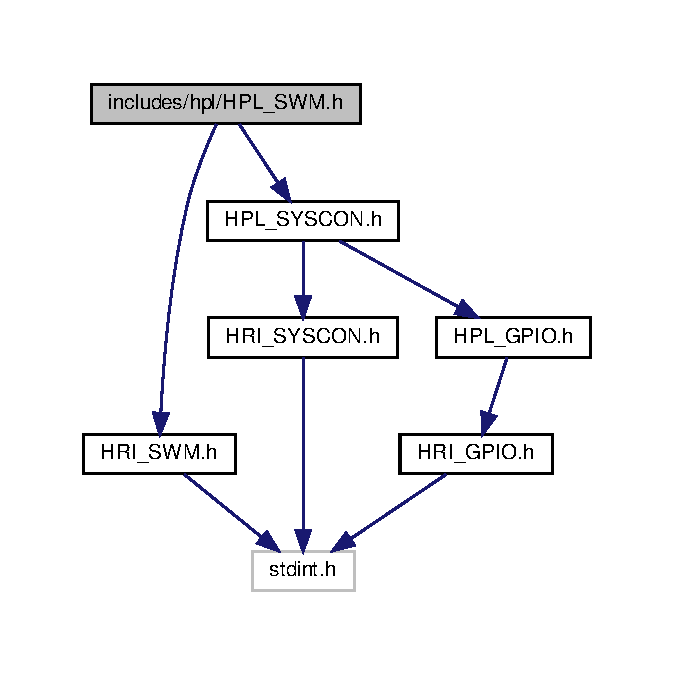
\includegraphics[width=324pt]{d1/d84/HPL__SWM_8h__incl}
\end{center}
\end{figure}
Gráfico de los archivos que directa o indirectamente incluyen a este archivo\+:\nopagebreak
\begin{figure}[H]
\begin{center}
\leavevmode
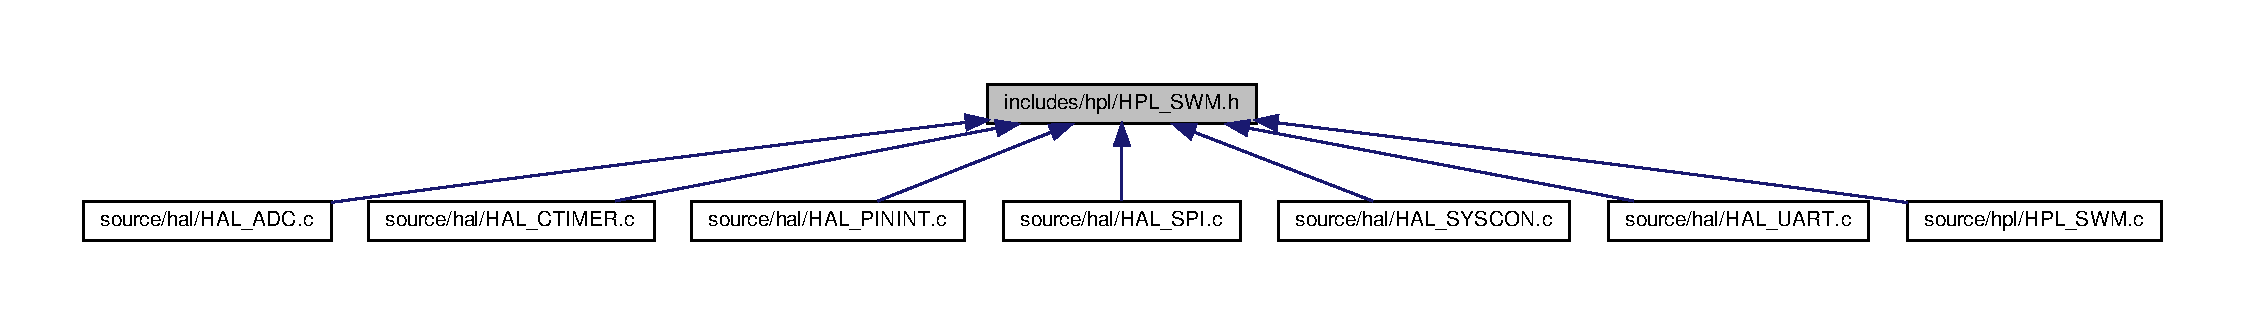
\includegraphics[width=350pt]{d1/deb/HPL__SWM_8h__dep__incl}
\end{center}
\end{figure}
\subsection*{Enumeraciones}
\begin{DoxyCompactItemize}
\item 
\mbox{\Hypertarget{HPL__SWM_8h_a142ac4728429e7b0212a2439cf625ba0}\label{HPL__SWM_8h_a142ac4728429e7b0212a2439cf625ba0}} 
enum {\bfseries S\+W\+M\+\_\+enable\+\_\+en} \{ {\bfseries S\+W\+M\+\_\+\+E\+N\+A\+B\+LE} = 0, 
{\bfseries S\+W\+M\+\_\+\+D\+I\+S\+A\+B\+LE}
 \}
\end{DoxyCompactItemize}
\subsection*{Funciones}
\begin{DoxyCompactItemize}
\item 
\mbox{\Hypertarget{HPL__SWM_8h_ac536db4465a4bde7b91e205ba619d878}\label{HPL__SWM_8h_ac536db4465a4bde7b91e205ba619d878}} 
static void \hyperlink{HPL__SWM_8h_ac536db4465a4bde7b91e205ba619d878}{S\+W\+M\+\_\+init} (void)
\begin{DoxyCompactList}\small\item\em Inicializacion de la Switch Matrix. \end{DoxyCompactList}\item 
\mbox{\Hypertarget{HPL__SWM_8h_a737f4936b853918bca089135d2827605}\label{HPL__SWM_8h_a737f4936b853918bca089135d2827605}} 
static void \hyperlink{HPL__SWM_8h_a737f4936b853918bca089135d2827605}{S\+W\+M\+\_\+deinit} (void)
\begin{DoxyCompactList}\small\item\em Deinicializacion de la Switch Matrix. \end{DoxyCompactList}\item 
static void \hyperlink{HPL__SWM_8h_a60f41fe1e4050d00e8b31bc90895f02a}{S\+W\+M\+\_\+assign\+\_\+uart\+\_\+\+T\+XD} (uint8\+\_\+t uart, uint8\+\_\+t port, uint8\+\_\+t pin)
\begin{DoxyCompactList}\small\item\em Asignar un pin del M\+CU a la funcion U\+A\+R\+Tn T\+XD. \end{DoxyCompactList}\item 
static void \hyperlink{HPL__SWM_8h_a2a9dd06c266b4a9f13422049ca6e8025}{S\+W\+M\+\_\+assign\+\_\+uart\+\_\+\+R\+XD} (uint8\+\_\+t uart, uint8\+\_\+t port, uint8\+\_\+t pin)
\begin{DoxyCompactList}\small\item\em Asignar un pin del M\+CU a la funcion U\+A\+R\+Tn R\+XD. \end{DoxyCompactList}\item 
static void \hyperlink{HPL__SWM_8h_a6c2d55563fe6dd686c582b01881eb09d}{S\+W\+M\+\_\+assign\+\_\+uart\+\_\+\+R\+TS} (uint8\+\_\+t uart, uint8\+\_\+t port, uint8\+\_\+t pin)
\begin{DoxyCompactList}\small\item\em Asignar un pin del M\+CU a la funcion U\+A\+R\+Tn R\+TS. \end{DoxyCompactList}\item 
static void \hyperlink{HPL__SWM_8h_ab5bb74a503e21e7e3069ca96ba061197}{S\+W\+M\+\_\+assign\+\_\+uart\+\_\+\+C\+TS} (uint8\+\_\+t uart, uint8\+\_\+t port, uint8\+\_\+t pin)
\begin{DoxyCompactList}\small\item\em Asignar un pin del M\+CU a la funcion U\+A\+R\+Tn C\+TS. \end{DoxyCompactList}\item 
static void \hyperlink{HPL__SWM_8h_a97f3b3c44e9a19948bde3a69b1570530}{S\+W\+M\+\_\+assign\+\_\+uart\+\_\+\+S\+C\+LK} (uint8\+\_\+t uart, uint8\+\_\+t port, uint8\+\_\+t pin)
\begin{DoxyCompactList}\small\item\em Asignar un pin del M\+CU a la funcion U\+A\+R\+Tn S\+C\+LK. \end{DoxyCompactList}\item 
static void \hyperlink{HPL__SWM_8h_ad43c4074fec877231656d1708c4c8007}{S\+W\+M\+\_\+assign\+\_\+spi\+\_\+\+S\+CK} (uint8\+\_\+t spi, uint8\+\_\+t port, uint8\+\_\+t pin)
\begin{DoxyCompactList}\small\item\em Asignar un pin del M\+CU a la funcion S\+P\+In S\+CK. \end{DoxyCompactList}\item 
static void \hyperlink{HPL__SWM_8h_a06d9be7bba0047142099f1e69518b12e}{S\+W\+M\+\_\+assign\+\_\+spi\+\_\+\+M\+O\+SI} (uint8\+\_\+t spi, uint8\+\_\+t port, uint8\+\_\+t pin)
\begin{DoxyCompactList}\small\item\em Asignar un pin del M\+CU a la funcion S\+P\+In M\+O\+SI. \end{DoxyCompactList}\item 
static void \hyperlink{HPL__SWM_8h_a51673fcfa7163686b764b44c17a95e8f}{S\+W\+M\+\_\+assign\+\_\+spi\+\_\+\+M\+I\+SO} (uint8\+\_\+t spi, uint8\+\_\+t port, uint8\+\_\+t pin)
\begin{DoxyCompactList}\small\item\em Asignar un pin del M\+CU a la funcion S\+P\+In M\+I\+SO. \end{DoxyCompactList}\item 
static void \hyperlink{HPL__SWM_8h_a39a3e2c4add6776b9beaa9501fd5443f}{S\+W\+M\+\_\+assign\+\_\+spi\+\_\+\+S\+S\+E\+L0} (uint8\+\_\+t spi, uint8\+\_\+t port, uint8\+\_\+t pin)
\begin{DoxyCompactList}\small\item\em Asignar un pin del M\+CU a la funcion S\+P\+In S\+S\+E\+L0. \end{DoxyCompactList}\item 
static void \hyperlink{HPL__SWM_8h_a2c412d2bc5d9285aab9581f4311792d8}{S\+W\+M\+\_\+assign\+\_\+spi\+\_\+\+S\+S\+E\+L1} (uint8\+\_\+t spi, uint8\+\_\+t port, uint8\+\_\+t pin)
\begin{DoxyCompactList}\small\item\em Asignar un pin del M\+CU a la funcion S\+P\+In S\+S\+E\+L1. \end{DoxyCompactList}\item 
static void \hyperlink{HPL__SWM_8h_a2238cb94f47a1d33563c1d714d7f213b}{S\+W\+M\+\_\+assign\+\_\+spi\+\_\+\+S\+S\+E\+L2} (uint8\+\_\+t spi, uint8\+\_\+t port, uint8\+\_\+t pin)
\begin{DoxyCompactList}\small\item\em Asignar un pin del M\+CU a la funcion S\+P\+In S\+S\+E\+L2. \end{DoxyCompactList}\item 
static void \hyperlink{HPL__SWM_8h_acc2b2ffbd6ff1343250abac19789f87e}{S\+W\+M\+\_\+assign\+\_\+spi\+\_\+\+S\+S\+E\+L3} (uint8\+\_\+t spi, uint8\+\_\+t port, uint8\+\_\+t pin)
\begin{DoxyCompactList}\small\item\em Asignar un pin del M\+CU a la funcion S\+P\+In S\+S\+E\+L3. \end{DoxyCompactList}\item 
static void \hyperlink{HPL__SWM_8h_a4e47fda85d3bc1f56153a39af4dd41e2}{S\+W\+M\+\_\+assign\+\_\+sct\+\_\+\+I\+N\+\_\+A} (uint8\+\_\+t port, uint8\+\_\+t pin)
\begin{DoxyCompactList}\small\item\em Asignar un pin del M\+CU a la funcion S\+CT I\+N\+\_\+A. \end{DoxyCompactList}\item 
static void \hyperlink{HPL__SWM_8h_a521309a78720cfb00c77151a8c31df94}{S\+W\+M\+\_\+assign\+\_\+sct\+\_\+\+I\+N\+\_\+B} (uint8\+\_\+t port, uint8\+\_\+t pin)
\begin{DoxyCompactList}\small\item\em Asignar un pin del M\+CU a la funcion S\+CT I\+N\+\_\+B. \end{DoxyCompactList}\item 
static void \hyperlink{HPL__SWM_8h_ab21907521c23026717862948ab0a1696}{S\+W\+M\+\_\+assign\+\_\+sct\+\_\+\+I\+N\+\_\+C} (uint8\+\_\+t port, uint8\+\_\+t pin)
\begin{DoxyCompactList}\small\item\em Asignar un pin del M\+CU a la funcion S\+CT I\+N\+\_\+C. \end{DoxyCompactList}\item 
static void \hyperlink{HPL__SWM_8h_a9330330d9ce67ceafbfa7e928516c44f}{S\+W\+M\+\_\+assign\+\_\+sct\+\_\+\+I\+N\+\_\+D} (uint8\+\_\+t port, uint8\+\_\+t pin)
\begin{DoxyCompactList}\small\item\em Asignar un pin del M\+CU a la funcion S\+CT I\+N\+\_\+D. \end{DoxyCompactList}\item 
static void \hyperlink{HPL__SWM_8h_ac1e884ebd779bcef41208320197466f5}{S\+W\+M\+\_\+assign\+\_\+sct\+\_\+\+O\+U\+T0} (uint8\+\_\+t port, uint8\+\_\+t pin)
\begin{DoxyCompactList}\small\item\em Asignar un pin del M\+CU a la funcion S\+CT O\+U\+T0. \end{DoxyCompactList}\item 
static void \hyperlink{HPL__SWM_8h_a5f8f4b3d47a77576c3b7ec2cfcca818d}{S\+W\+M\+\_\+assign\+\_\+sct\+\_\+\+O\+U\+T1} (uint8\+\_\+t port, uint8\+\_\+t pin)
\begin{DoxyCompactList}\small\item\em Asignar un pin del M\+CU a la funcion S\+CT O\+U\+T1. \end{DoxyCompactList}\item 
static void \hyperlink{HPL__SWM_8h_a86063ff7fa029a8f68beb41de0033871}{S\+W\+M\+\_\+assign\+\_\+sct\+\_\+\+O\+U\+T2} (uint8\+\_\+t port, uint8\+\_\+t pin)
\begin{DoxyCompactList}\small\item\em Asignar un pin del M\+CU a la funcion S\+CT O\+U\+T2. \end{DoxyCompactList}\item 
static void \hyperlink{HPL__SWM_8h_a53825ed720ffcfcf8587e73281fddb2c}{S\+W\+M\+\_\+assign\+\_\+sct\+\_\+\+O\+U\+T3} (uint8\+\_\+t port, uint8\+\_\+t pin)
\begin{DoxyCompactList}\small\item\em Asignar un pin del M\+CU a la funcion S\+CT O\+U\+T3. \end{DoxyCompactList}\item 
static void \hyperlink{HPL__SWM_8h_a646eba307482f12899371218a35b783c}{S\+W\+M\+\_\+assign\+\_\+sct\+\_\+\+O\+U\+T4} (uint8\+\_\+t port, uint8\+\_\+t pin)
\begin{DoxyCompactList}\small\item\em Asignar un pin del M\+CU a la funcion S\+CT O\+U\+T4. \end{DoxyCompactList}\item 
static void \hyperlink{HPL__SWM_8h_a60502954a455881f0b5a163da323ef2e}{S\+W\+M\+\_\+assign\+\_\+sct\+\_\+\+O\+U\+T5} (uint8\+\_\+t port, uint8\+\_\+t pin)
\begin{DoxyCompactList}\small\item\em Asignar un pin del M\+CU a la funcion S\+CT O\+U\+T5. \end{DoxyCompactList}\item 
static void \hyperlink{HPL__SWM_8h_ae2a8e178b9905df0c6e137d5920c38a7}{S\+W\+M\+\_\+assign\+\_\+sct\+\_\+\+O\+U\+T6} (uint8\+\_\+t port, uint8\+\_\+t pin)
\begin{DoxyCompactList}\small\item\em Asignar un pin del M\+CU a la funcion S\+CT O\+U\+T6. \end{DoxyCompactList}\item 
static void \hyperlink{HPL__SWM_8h_aedd50341001a6d2af785250d5e8d12a6}{S\+W\+M\+\_\+assign\+\_\+iic\+\_\+\+S\+DA} (uint8\+\_\+t iic, uint8\+\_\+t port, uint8\+\_\+t pin)
\begin{DoxyCompactList}\small\item\em Asignar un pin del M\+CU a la funcion I\+I\+Cn S\+DA. \end{DoxyCompactList}\item 
static void \hyperlink{HPL__SWM_8h_a494e8a2065357cfc55b30059c3909609}{S\+W\+M\+\_\+assign\+\_\+iic\+\_\+\+S\+CL} (uint8\+\_\+t iic, uint8\+\_\+t port, uint8\+\_\+t pin)
\begin{DoxyCompactList}\small\item\em Asignar un pin del M\+CU a la funcion I\+I\+Cn S\+CL. \end{DoxyCompactList}\item 
static void \hyperlink{HPL__SWM_8h_ae9ec78f27020beaae4049407294be86c}{S\+W\+M\+\_\+assign\+\_\+\+C\+O\+M\+P0\+\_\+\+O\+UT} (uint8\+\_\+t port, uint8\+\_\+t pin)
\begin{DoxyCompactList}\small\item\em Asignar un pin del M\+CU a la funcion C\+O\+M\+P0 O\+UT. \end{DoxyCompactList}\item 
static void \hyperlink{HPL__SWM_8h_a3e1c96ae214454bf541df45189c5bc89}{S\+W\+M\+\_\+assign\+\_\+\+C\+L\+K\+O\+UT} (uint8\+\_\+t port, uint8\+\_\+t pin)
\begin{DoxyCompactList}\small\item\em Asignar un pin del M\+CU a la funcion C\+L\+K\+O\+UT. \end{DoxyCompactList}\item 
static void \hyperlink{HPL__SWM_8h_ae93da114f52224d70be758d8e86f2ba0}{S\+W\+M\+\_\+assign\+\_\+\+I\+N\+T\+\_\+\+B\+M\+AT} (uint8\+\_\+t port, uint8\+\_\+t pin)
\begin{DoxyCompactList}\small\item\em Asignar un pin del M\+CU a la funcion I\+NT B\+M\+AT. \end{DoxyCompactList}\item 
static void \hyperlink{HPL__SWM_8h_a1c63006c19ab20b7826bf651a0e7dcad}{S\+W\+M\+\_\+assign\+\_\+\+T0\+\_\+\+M\+AT} (uint8\+\_\+t mat, uint8\+\_\+t port, uint8\+\_\+t pin)
\begin{DoxyCompactList}\small\item\em Asignar un pin del M\+CU a la funcion T0 M\+A\+Tn. \end{DoxyCompactList}\item 
static void \hyperlink{HPL__SWM_8h_afc9b4382b09dab73bea590322aaef313}{S\+W\+M\+\_\+assign\+\_\+\+T0\+\_\+\+C\+AP} (uint8\+\_\+t cap, uint8\+\_\+t port, uint8\+\_\+t pin)
\begin{DoxyCompactList}\small\item\em Asignar un pin del M\+CU a la funcion T0 C\+A\+Pn. \end{DoxyCompactList}\item 
static void \hyperlink{HPL__SWM_8h_ac24a18ebef94b9d39b8cf1494f9ac21e}{S\+W\+M\+\_\+enable\+\_\+\+A\+C\+MP} (uint8\+\_\+t acmp, S\+W\+M\+\_\+enable\+\_\+en en\+\_\+dis)
\begin{DoxyCompactList}\small\item\em Habilitar/inhabilitar la funcion A\+C\+M\+Pn. \end{DoxyCompactList}\item 
static void \hyperlink{HPL__SWM_8h_a39bd0a4ec28fa0d0385f58d38b016d54}{S\+W\+M\+\_\+enable\+\_\+\+S\+W\+C\+LK} (S\+W\+M\+\_\+enable\+\_\+en en\+\_\+dis)
\begin{DoxyCompactList}\small\item\em Habilitar/inhabilitar la funcion S\+W\+C\+LK. \end{DoxyCompactList}\item 
static void \hyperlink{HPL__SWM_8h_aaa30ac5a05823874719a55e8a727093b}{S\+W\+M\+\_\+enable\+\_\+\+S\+W\+D\+IO} (S\+W\+M\+\_\+enable\+\_\+en en\+\_\+dis)
\begin{DoxyCompactList}\small\item\em Habilitar/inhabilitar la funcion S\+W\+D\+IO. \end{DoxyCompactList}\item 
static void \hyperlink{HPL__SWM_8h_aa28bd697cfec3ccf2e69ec68ccbe2fd0}{S\+W\+M\+\_\+enable\+\_\+\+X\+T\+A\+L\+IN} (S\+W\+M\+\_\+enable\+\_\+en en\+\_\+dis)
\begin{DoxyCompactList}\small\item\em Habilitar/inhabilitar la funcion X\+T\+A\+L\+IN. \end{DoxyCompactList}\item 
static void \hyperlink{HPL__SWM_8h_af26a23c5affe7c4011c90ada19a063a7}{S\+W\+M\+\_\+enable\+\_\+\+X\+T\+A\+L\+O\+UT} (S\+W\+M\+\_\+enable\+\_\+en en\+\_\+dis)
\begin{DoxyCompactList}\small\item\em Habilitar/inhabilitar la funcion X\+T\+A\+L\+O\+UT. \end{DoxyCompactList}\item 
static void \hyperlink{HPL__SWM_8h_aeb886e9841975315d82d350b7687306a}{S\+W\+M\+\_\+enable\+\_\+\+R\+E\+S\+E\+TN} (S\+W\+M\+\_\+enable\+\_\+en en\+\_\+dis)
\begin{DoxyCompactList}\small\item\em Habilitar/inhabilitar la funcion R\+E\+S\+E\+TN. \end{DoxyCompactList}\item 
static void \hyperlink{HPL__SWM_8h_ac766a6eb91ec9bead6db08904fef786d}{S\+W\+M\+\_\+enable\+\_\+\+C\+L\+K\+IN} (S\+W\+M\+\_\+enable\+\_\+en en\+\_\+dis)
\begin{DoxyCompactList}\small\item\em Habilitar/inhabilitar la funcion C\+L\+K\+IN. \end{DoxyCompactList}\item 
static void \hyperlink{HPL__SWM_8h_a71d06bef68604d4c3af51a2d5e436d64}{S\+W\+M\+\_\+enable\+\_\+\+V\+D\+D\+C\+MP} (S\+W\+M\+\_\+enable\+\_\+en en\+\_\+dis)
\begin{DoxyCompactList}\small\item\em Habilitar/inhabilitar la funcion V\+D\+D\+C\+MP. \end{DoxyCompactList}\item 
static void \hyperlink{HPL__SWM_8h_a601e78a53ab107d417c744e43bb71213}{S\+W\+M\+\_\+enable\+\_\+\+A\+DC} (uint8\+\_\+t adc, S\+W\+M\+\_\+enable\+\_\+en en\+\_\+dis)
\begin{DoxyCompactList}\small\item\em Habilitar/inhabilitar la funcion A\+DC. \end{DoxyCompactList}\item 
static void \hyperlink{HPL__SWM_8h_ae12e3e59db0d3bd4a17d0e200db3e564}{S\+W\+M\+\_\+enable\+\_\+\+D\+AC} (uint8\+\_\+t dac, S\+W\+M\+\_\+enable\+\_\+en en\+\_\+dis)
\begin{DoxyCompactList}\small\item\em Habilitar/inhabilitar la funcion D\+AC. \end{DoxyCompactList}\item 
static void \hyperlink{HPL__SWM_8h_a3e486973cbba94c52ed5245862a32fa7}{S\+W\+M\+\_\+enable\+\_\+\+C\+A\+P\+TX} (uint8\+\_\+t captx, S\+W\+M\+\_\+enable\+\_\+en en\+\_\+dis)
\begin{DoxyCompactList}\small\item\em Habilitar/inhabilitar la funcion C\+A\+P\+TX. \end{DoxyCompactList}\item 
static void \hyperlink{HPL__SWM_8h_a11956351694500dfa54078b75ab0fb16}{S\+W\+M\+\_\+enable\+\_\+\+C\+A\+P\+YL} (S\+W\+M\+\_\+enable\+\_\+en en\+\_\+dis)
\begin{DoxyCompactList}\small\item\em Habilitar/inhabilitar la funcion C\+A\+P\+YL. \end{DoxyCompactList}\item 
static void \hyperlink{HPL__SWM_8h_a251a79c9590da5718e29b1c2b6a01cc0}{S\+W\+M\+\_\+enable\+\_\+\+C\+A\+P\+YH} (S\+W\+M\+\_\+enable\+\_\+en en\+\_\+dis)
\begin{DoxyCompactList}\small\item\em Habilitar/inhabilitar la funcion C\+A\+P\+YH. \end{DoxyCompactList}\end{DoxyCompactItemize}
\subsection*{Variables}
\begin{DoxyCompactItemize}
\item 
\mbox{\Hypertarget{HPL__SWM_8h_a79cbaf1ff3c7132e45e5198f4ab6e149}\label{HPL__SWM_8h_a79cbaf1ff3c7132e45e5198f4ab6e149}} 
volatile \hyperlink{HRI__SWM_8h_d0/db2/structSWM__per__t}{S\+W\+M\+\_\+per\+\_\+t} $\ast$const \hyperlink{HPL__SWM_8h_a79cbaf1ff3c7132e45e5198f4ab6e149}{S\+WM}
\begin{DoxyCompactList}\small\item\em Periferico S\+WM. \end{DoxyCompactList}\end{DoxyCompactItemize}


\subsection{Descripción detallada}
Definiciones a nivel de periferico del modulo S\+WM (L\+P\+C845) 

\begin{DoxyAuthor}{Autor}
Augusto Santini 
\end{DoxyAuthor}
\begin{DoxyDate}{Fecha}
3/2020 
\end{DoxyDate}
\begin{DoxyVersion}{Versión}
1.\+0 
\end{DoxyVersion}


\subsection{Documentación de las funciones}
\mbox{\Hypertarget{HPL__SWM_8h_a60f41fe1e4050d00e8b31bc90895f02a}\label{HPL__SWM_8h_a60f41fe1e4050d00e8b31bc90895f02a}} 
\index{H\+P\+L\+\_\+\+S\+W\+M.\+h@{H\+P\+L\+\_\+\+S\+W\+M.\+h}!S\+W\+M\+\_\+assign\+\_\+uart\+\_\+\+T\+XD@{S\+W\+M\+\_\+assign\+\_\+uart\+\_\+\+T\+XD}}
\index{S\+W\+M\+\_\+assign\+\_\+uart\+\_\+\+T\+XD@{S\+W\+M\+\_\+assign\+\_\+uart\+\_\+\+T\+XD}!H\+P\+L\+\_\+\+S\+W\+M.\+h@{H\+P\+L\+\_\+\+S\+W\+M.\+h}}
\subsubsection{\texorpdfstring{S\+W\+M\+\_\+assign\+\_\+uart\+\_\+\+T\+X\+D()}{SWM\_assign\_uart\_TXD()}}
{\footnotesize\ttfamily static void S\+W\+M\+\_\+assign\+\_\+uart\+\_\+\+T\+XD (\begin{DoxyParamCaption}\item[{uint8\+\_\+t}]{uart,  }\item[{uint8\+\_\+t}]{port,  }\item[{uint8\+\_\+t}]{pin }\end{DoxyParamCaption})\hspace{0.3cm}{\ttfamily [inline]}, {\ttfamily [static]}}



Asignar un pin del M\+CU a la funcion U\+A\+R\+Tn T\+XD. 


\begin{DoxyParams}[1]{Parámetros}
\mbox{\tt in}  & {\em uart} & Instancia de U\+A\+RT a la cual asignar \\
\hline
\mbox{\tt in}  & {\em port} & Numero de puerto a asignar \\
\hline
\mbox{\tt in}  & {\em pin} & Numero de pin a asignar \\
\hline
\end{DoxyParams}
\mbox{\Hypertarget{HPL__SWM_8h_a2a9dd06c266b4a9f13422049ca6e8025}\label{HPL__SWM_8h_a2a9dd06c266b4a9f13422049ca6e8025}} 
\index{H\+P\+L\+\_\+\+S\+W\+M.\+h@{H\+P\+L\+\_\+\+S\+W\+M.\+h}!S\+W\+M\+\_\+assign\+\_\+uart\+\_\+\+R\+XD@{S\+W\+M\+\_\+assign\+\_\+uart\+\_\+\+R\+XD}}
\index{S\+W\+M\+\_\+assign\+\_\+uart\+\_\+\+R\+XD@{S\+W\+M\+\_\+assign\+\_\+uart\+\_\+\+R\+XD}!H\+P\+L\+\_\+\+S\+W\+M.\+h@{H\+P\+L\+\_\+\+S\+W\+M.\+h}}
\subsubsection{\texorpdfstring{S\+W\+M\+\_\+assign\+\_\+uart\+\_\+\+R\+X\+D()}{SWM\_assign\_uart\_RXD()}}
{\footnotesize\ttfamily static void S\+W\+M\+\_\+assign\+\_\+uart\+\_\+\+R\+XD (\begin{DoxyParamCaption}\item[{uint8\+\_\+t}]{uart,  }\item[{uint8\+\_\+t}]{port,  }\item[{uint8\+\_\+t}]{pin }\end{DoxyParamCaption})\hspace{0.3cm}{\ttfamily [inline]}, {\ttfamily [static]}}



Asignar un pin del M\+CU a la funcion U\+A\+R\+Tn R\+XD. 


\begin{DoxyParams}[1]{Parámetros}
\mbox{\tt in}  & {\em uart} & Instancia de U\+A\+RT a la cual asignar \\
\hline
\mbox{\tt in}  & {\em port} & Numero de puerto a asignar \\
\hline
\mbox{\tt in}  & {\em pin} & Numero de pin a asignar \\
\hline
\end{DoxyParams}
\mbox{\Hypertarget{HPL__SWM_8h_a6c2d55563fe6dd686c582b01881eb09d}\label{HPL__SWM_8h_a6c2d55563fe6dd686c582b01881eb09d}} 
\index{H\+P\+L\+\_\+\+S\+W\+M.\+h@{H\+P\+L\+\_\+\+S\+W\+M.\+h}!S\+W\+M\+\_\+assign\+\_\+uart\+\_\+\+R\+TS@{S\+W\+M\+\_\+assign\+\_\+uart\+\_\+\+R\+TS}}
\index{S\+W\+M\+\_\+assign\+\_\+uart\+\_\+\+R\+TS@{S\+W\+M\+\_\+assign\+\_\+uart\+\_\+\+R\+TS}!H\+P\+L\+\_\+\+S\+W\+M.\+h@{H\+P\+L\+\_\+\+S\+W\+M.\+h}}
\subsubsection{\texorpdfstring{S\+W\+M\+\_\+assign\+\_\+uart\+\_\+\+R\+T\+S()}{SWM\_assign\_uart\_RTS()}}
{\footnotesize\ttfamily static void S\+W\+M\+\_\+assign\+\_\+uart\+\_\+\+R\+TS (\begin{DoxyParamCaption}\item[{uint8\+\_\+t}]{uart,  }\item[{uint8\+\_\+t}]{port,  }\item[{uint8\+\_\+t}]{pin }\end{DoxyParamCaption})\hspace{0.3cm}{\ttfamily [inline]}, {\ttfamily [static]}}



Asignar un pin del M\+CU a la funcion U\+A\+R\+Tn R\+TS. 


\begin{DoxyParams}[1]{Parámetros}
\mbox{\tt in}  & {\em uart} & Instancia de U\+A\+RT a la cual asignar \\
\hline
\mbox{\tt in}  & {\em port} & Numero de puerto a asignar \\
\hline
\mbox{\tt in}  & {\em pin} & Numero de pin a asignar \\
\hline
\end{DoxyParams}
\mbox{\Hypertarget{HPL__SWM_8h_ab5bb74a503e21e7e3069ca96ba061197}\label{HPL__SWM_8h_ab5bb74a503e21e7e3069ca96ba061197}} 
\index{H\+P\+L\+\_\+\+S\+W\+M.\+h@{H\+P\+L\+\_\+\+S\+W\+M.\+h}!S\+W\+M\+\_\+assign\+\_\+uart\+\_\+\+C\+TS@{S\+W\+M\+\_\+assign\+\_\+uart\+\_\+\+C\+TS}}
\index{S\+W\+M\+\_\+assign\+\_\+uart\+\_\+\+C\+TS@{S\+W\+M\+\_\+assign\+\_\+uart\+\_\+\+C\+TS}!H\+P\+L\+\_\+\+S\+W\+M.\+h@{H\+P\+L\+\_\+\+S\+W\+M.\+h}}
\subsubsection{\texorpdfstring{S\+W\+M\+\_\+assign\+\_\+uart\+\_\+\+C\+T\+S()}{SWM\_assign\_uart\_CTS()}}
{\footnotesize\ttfamily static void S\+W\+M\+\_\+assign\+\_\+uart\+\_\+\+C\+TS (\begin{DoxyParamCaption}\item[{uint8\+\_\+t}]{uart,  }\item[{uint8\+\_\+t}]{port,  }\item[{uint8\+\_\+t}]{pin }\end{DoxyParamCaption})\hspace{0.3cm}{\ttfamily [inline]}, {\ttfamily [static]}}



Asignar un pin del M\+CU a la funcion U\+A\+R\+Tn C\+TS. 


\begin{DoxyParams}[1]{Parámetros}
\mbox{\tt in}  & {\em uart} & Instancia de U\+A\+RT a la cual asignar \\
\hline
\mbox{\tt in}  & {\em port} & Numero de puerto a asignar \\
\hline
\mbox{\tt in}  & {\em pin} & Numero de pin a asignar \\
\hline
\end{DoxyParams}
\mbox{\Hypertarget{HPL__SWM_8h_a97f3b3c44e9a19948bde3a69b1570530}\label{HPL__SWM_8h_a97f3b3c44e9a19948bde3a69b1570530}} 
\index{H\+P\+L\+\_\+\+S\+W\+M.\+h@{H\+P\+L\+\_\+\+S\+W\+M.\+h}!S\+W\+M\+\_\+assign\+\_\+uart\+\_\+\+S\+C\+LK@{S\+W\+M\+\_\+assign\+\_\+uart\+\_\+\+S\+C\+LK}}
\index{S\+W\+M\+\_\+assign\+\_\+uart\+\_\+\+S\+C\+LK@{S\+W\+M\+\_\+assign\+\_\+uart\+\_\+\+S\+C\+LK}!H\+P\+L\+\_\+\+S\+W\+M.\+h@{H\+P\+L\+\_\+\+S\+W\+M.\+h}}
\subsubsection{\texorpdfstring{S\+W\+M\+\_\+assign\+\_\+uart\+\_\+\+S\+C\+L\+K()}{SWM\_assign\_uart\_SCLK()}}
{\footnotesize\ttfamily static void S\+W\+M\+\_\+assign\+\_\+uart\+\_\+\+S\+C\+LK (\begin{DoxyParamCaption}\item[{uint8\+\_\+t}]{uart,  }\item[{uint8\+\_\+t}]{port,  }\item[{uint8\+\_\+t}]{pin }\end{DoxyParamCaption})\hspace{0.3cm}{\ttfamily [inline]}, {\ttfamily [static]}}



Asignar un pin del M\+CU a la funcion U\+A\+R\+Tn S\+C\+LK. 


\begin{DoxyParams}[1]{Parámetros}
\mbox{\tt in}  & {\em uart} & Instancia de U\+A\+RT a la cual asignar \\
\hline
\mbox{\tt in}  & {\em port} & Numero de puerto a asignar \\
\hline
\mbox{\tt in}  & {\em pin} & Numero de pin a asignar \\
\hline
\end{DoxyParams}
\mbox{\Hypertarget{HPL__SWM_8h_ad43c4074fec877231656d1708c4c8007}\label{HPL__SWM_8h_ad43c4074fec877231656d1708c4c8007}} 
\index{H\+P\+L\+\_\+\+S\+W\+M.\+h@{H\+P\+L\+\_\+\+S\+W\+M.\+h}!S\+W\+M\+\_\+assign\+\_\+spi\+\_\+\+S\+CK@{S\+W\+M\+\_\+assign\+\_\+spi\+\_\+\+S\+CK}}
\index{S\+W\+M\+\_\+assign\+\_\+spi\+\_\+\+S\+CK@{S\+W\+M\+\_\+assign\+\_\+spi\+\_\+\+S\+CK}!H\+P\+L\+\_\+\+S\+W\+M.\+h@{H\+P\+L\+\_\+\+S\+W\+M.\+h}}
\subsubsection{\texorpdfstring{S\+W\+M\+\_\+assign\+\_\+spi\+\_\+\+S\+C\+K()}{SWM\_assign\_spi\_SCK()}}
{\footnotesize\ttfamily static void S\+W\+M\+\_\+assign\+\_\+spi\+\_\+\+S\+CK (\begin{DoxyParamCaption}\item[{uint8\+\_\+t}]{spi,  }\item[{uint8\+\_\+t}]{port,  }\item[{uint8\+\_\+t}]{pin }\end{DoxyParamCaption})\hspace{0.3cm}{\ttfamily [inline]}, {\ttfamily [static]}}



Asignar un pin del M\+CU a la funcion S\+P\+In S\+CK. 


\begin{DoxyParams}[1]{Parámetros}
\mbox{\tt in}  & {\em spi} & Instancia de S\+PI a la cual asignar \\
\hline
\mbox{\tt in}  & {\em port} & Numero de puerto a asignar \\
\hline
\mbox{\tt in}  & {\em pin} & Numero de pin a asignar \\
\hline
\end{DoxyParams}
\mbox{\Hypertarget{HPL__SWM_8h_a06d9be7bba0047142099f1e69518b12e}\label{HPL__SWM_8h_a06d9be7bba0047142099f1e69518b12e}} 
\index{H\+P\+L\+\_\+\+S\+W\+M.\+h@{H\+P\+L\+\_\+\+S\+W\+M.\+h}!S\+W\+M\+\_\+assign\+\_\+spi\+\_\+\+M\+O\+SI@{S\+W\+M\+\_\+assign\+\_\+spi\+\_\+\+M\+O\+SI}}
\index{S\+W\+M\+\_\+assign\+\_\+spi\+\_\+\+M\+O\+SI@{S\+W\+M\+\_\+assign\+\_\+spi\+\_\+\+M\+O\+SI}!H\+P\+L\+\_\+\+S\+W\+M.\+h@{H\+P\+L\+\_\+\+S\+W\+M.\+h}}
\subsubsection{\texorpdfstring{S\+W\+M\+\_\+assign\+\_\+spi\+\_\+\+M\+O\+S\+I()}{SWM\_assign\_spi\_MOSI()}}
{\footnotesize\ttfamily static void S\+W\+M\+\_\+assign\+\_\+spi\+\_\+\+M\+O\+SI (\begin{DoxyParamCaption}\item[{uint8\+\_\+t}]{spi,  }\item[{uint8\+\_\+t}]{port,  }\item[{uint8\+\_\+t}]{pin }\end{DoxyParamCaption})\hspace{0.3cm}{\ttfamily [inline]}, {\ttfamily [static]}}



Asignar un pin del M\+CU a la funcion S\+P\+In M\+O\+SI. 


\begin{DoxyParams}[1]{Parámetros}
\mbox{\tt in}  & {\em spi} & Instancia de S\+PI a la cual asignar \\
\hline
\mbox{\tt in}  & {\em port} & Numero de puerto a asignar \\
\hline
\mbox{\tt in}  & {\em pin} & Numero de pin a asignar \\
\hline
\end{DoxyParams}
\mbox{\Hypertarget{HPL__SWM_8h_a51673fcfa7163686b764b44c17a95e8f}\label{HPL__SWM_8h_a51673fcfa7163686b764b44c17a95e8f}} 
\index{H\+P\+L\+\_\+\+S\+W\+M.\+h@{H\+P\+L\+\_\+\+S\+W\+M.\+h}!S\+W\+M\+\_\+assign\+\_\+spi\+\_\+\+M\+I\+SO@{S\+W\+M\+\_\+assign\+\_\+spi\+\_\+\+M\+I\+SO}}
\index{S\+W\+M\+\_\+assign\+\_\+spi\+\_\+\+M\+I\+SO@{S\+W\+M\+\_\+assign\+\_\+spi\+\_\+\+M\+I\+SO}!H\+P\+L\+\_\+\+S\+W\+M.\+h@{H\+P\+L\+\_\+\+S\+W\+M.\+h}}
\subsubsection{\texorpdfstring{S\+W\+M\+\_\+assign\+\_\+spi\+\_\+\+M\+I\+S\+O()}{SWM\_assign\_spi\_MISO()}}
{\footnotesize\ttfamily static void S\+W\+M\+\_\+assign\+\_\+spi\+\_\+\+M\+I\+SO (\begin{DoxyParamCaption}\item[{uint8\+\_\+t}]{spi,  }\item[{uint8\+\_\+t}]{port,  }\item[{uint8\+\_\+t}]{pin }\end{DoxyParamCaption})\hspace{0.3cm}{\ttfamily [inline]}, {\ttfamily [static]}}



Asignar un pin del M\+CU a la funcion S\+P\+In M\+I\+SO. 


\begin{DoxyParams}[1]{Parámetros}
\mbox{\tt in}  & {\em spi} & Instancia de S\+PI a la cual asignar \\
\hline
\mbox{\tt in}  & {\em port} & Numero de puerto a asignar \\
\hline
\mbox{\tt in}  & {\em pin} & Numero de pin a asignar \\
\hline
\end{DoxyParams}
\mbox{\Hypertarget{HPL__SWM_8h_a39a3e2c4add6776b9beaa9501fd5443f}\label{HPL__SWM_8h_a39a3e2c4add6776b9beaa9501fd5443f}} 
\index{H\+P\+L\+\_\+\+S\+W\+M.\+h@{H\+P\+L\+\_\+\+S\+W\+M.\+h}!S\+W\+M\+\_\+assign\+\_\+spi\+\_\+\+S\+S\+E\+L0@{S\+W\+M\+\_\+assign\+\_\+spi\+\_\+\+S\+S\+E\+L0}}
\index{S\+W\+M\+\_\+assign\+\_\+spi\+\_\+\+S\+S\+E\+L0@{S\+W\+M\+\_\+assign\+\_\+spi\+\_\+\+S\+S\+E\+L0}!H\+P\+L\+\_\+\+S\+W\+M.\+h@{H\+P\+L\+\_\+\+S\+W\+M.\+h}}
\subsubsection{\texorpdfstring{S\+W\+M\+\_\+assign\+\_\+spi\+\_\+\+S\+S\+E\+L0()}{SWM\_assign\_spi\_SSEL0()}}
{\footnotesize\ttfamily static void S\+W\+M\+\_\+assign\+\_\+spi\+\_\+\+S\+S\+E\+L0 (\begin{DoxyParamCaption}\item[{uint8\+\_\+t}]{spi,  }\item[{uint8\+\_\+t}]{port,  }\item[{uint8\+\_\+t}]{pin }\end{DoxyParamCaption})\hspace{0.3cm}{\ttfamily [inline]}, {\ttfamily [static]}}



Asignar un pin del M\+CU a la funcion S\+P\+In S\+S\+E\+L0. 


\begin{DoxyParams}[1]{Parámetros}
\mbox{\tt in}  & {\em spi} & Instancia de S\+PI a la cual asignar \\
\hline
\mbox{\tt in}  & {\em port} & Numero de puerto a asignar \\
\hline
\mbox{\tt in}  & {\em pin} & Numero de pin a asignar \\
\hline
\end{DoxyParams}
\mbox{\Hypertarget{HPL__SWM_8h_a2c412d2bc5d9285aab9581f4311792d8}\label{HPL__SWM_8h_a2c412d2bc5d9285aab9581f4311792d8}} 
\index{H\+P\+L\+\_\+\+S\+W\+M.\+h@{H\+P\+L\+\_\+\+S\+W\+M.\+h}!S\+W\+M\+\_\+assign\+\_\+spi\+\_\+\+S\+S\+E\+L1@{S\+W\+M\+\_\+assign\+\_\+spi\+\_\+\+S\+S\+E\+L1}}
\index{S\+W\+M\+\_\+assign\+\_\+spi\+\_\+\+S\+S\+E\+L1@{S\+W\+M\+\_\+assign\+\_\+spi\+\_\+\+S\+S\+E\+L1}!H\+P\+L\+\_\+\+S\+W\+M.\+h@{H\+P\+L\+\_\+\+S\+W\+M.\+h}}
\subsubsection{\texorpdfstring{S\+W\+M\+\_\+assign\+\_\+spi\+\_\+\+S\+S\+E\+L1()}{SWM\_assign\_spi\_SSEL1()}}
{\footnotesize\ttfamily static void S\+W\+M\+\_\+assign\+\_\+spi\+\_\+\+S\+S\+E\+L1 (\begin{DoxyParamCaption}\item[{uint8\+\_\+t}]{spi,  }\item[{uint8\+\_\+t}]{port,  }\item[{uint8\+\_\+t}]{pin }\end{DoxyParamCaption})\hspace{0.3cm}{\ttfamily [inline]}, {\ttfamily [static]}}



Asignar un pin del M\+CU a la funcion S\+P\+In S\+S\+E\+L1. 


\begin{DoxyParams}[1]{Parámetros}
\mbox{\tt in}  & {\em spi} & Instancia de S\+PI a la cual asignar \\
\hline
\mbox{\tt in}  & {\em port} & Numero de puerto a asignar \\
\hline
\mbox{\tt in}  & {\em pin} & Numero de pin a asignar \\
\hline
\end{DoxyParams}
\mbox{\Hypertarget{HPL__SWM_8h_a2238cb94f47a1d33563c1d714d7f213b}\label{HPL__SWM_8h_a2238cb94f47a1d33563c1d714d7f213b}} 
\index{H\+P\+L\+\_\+\+S\+W\+M.\+h@{H\+P\+L\+\_\+\+S\+W\+M.\+h}!S\+W\+M\+\_\+assign\+\_\+spi\+\_\+\+S\+S\+E\+L2@{S\+W\+M\+\_\+assign\+\_\+spi\+\_\+\+S\+S\+E\+L2}}
\index{S\+W\+M\+\_\+assign\+\_\+spi\+\_\+\+S\+S\+E\+L2@{S\+W\+M\+\_\+assign\+\_\+spi\+\_\+\+S\+S\+E\+L2}!H\+P\+L\+\_\+\+S\+W\+M.\+h@{H\+P\+L\+\_\+\+S\+W\+M.\+h}}
\subsubsection{\texorpdfstring{S\+W\+M\+\_\+assign\+\_\+spi\+\_\+\+S\+S\+E\+L2()}{SWM\_assign\_spi\_SSEL2()}}
{\footnotesize\ttfamily static void S\+W\+M\+\_\+assign\+\_\+spi\+\_\+\+S\+S\+E\+L2 (\begin{DoxyParamCaption}\item[{uint8\+\_\+t}]{spi,  }\item[{uint8\+\_\+t}]{port,  }\item[{uint8\+\_\+t}]{pin }\end{DoxyParamCaption})\hspace{0.3cm}{\ttfamily [inline]}, {\ttfamily [static]}}



Asignar un pin del M\+CU a la funcion S\+P\+In S\+S\+E\+L2. 


\begin{DoxyParams}[1]{Parámetros}
\mbox{\tt in}  & {\em spi} & Instancia de S\+PI a la cual asignar \\
\hline
\mbox{\tt in}  & {\em port} & Numero de puerto a asignar \\
\hline
\mbox{\tt in}  & {\em pin} & Numero de pin a asignar \\
\hline
\end{DoxyParams}
\mbox{\Hypertarget{HPL__SWM_8h_acc2b2ffbd6ff1343250abac19789f87e}\label{HPL__SWM_8h_acc2b2ffbd6ff1343250abac19789f87e}} 
\index{H\+P\+L\+\_\+\+S\+W\+M.\+h@{H\+P\+L\+\_\+\+S\+W\+M.\+h}!S\+W\+M\+\_\+assign\+\_\+spi\+\_\+\+S\+S\+E\+L3@{S\+W\+M\+\_\+assign\+\_\+spi\+\_\+\+S\+S\+E\+L3}}
\index{S\+W\+M\+\_\+assign\+\_\+spi\+\_\+\+S\+S\+E\+L3@{S\+W\+M\+\_\+assign\+\_\+spi\+\_\+\+S\+S\+E\+L3}!H\+P\+L\+\_\+\+S\+W\+M.\+h@{H\+P\+L\+\_\+\+S\+W\+M.\+h}}
\subsubsection{\texorpdfstring{S\+W\+M\+\_\+assign\+\_\+spi\+\_\+\+S\+S\+E\+L3()}{SWM\_assign\_spi\_SSEL3()}}
{\footnotesize\ttfamily static void S\+W\+M\+\_\+assign\+\_\+spi\+\_\+\+S\+S\+E\+L3 (\begin{DoxyParamCaption}\item[{uint8\+\_\+t}]{spi,  }\item[{uint8\+\_\+t}]{port,  }\item[{uint8\+\_\+t}]{pin }\end{DoxyParamCaption})\hspace{0.3cm}{\ttfamily [inline]}, {\ttfamily [static]}}



Asignar un pin del M\+CU a la funcion S\+P\+In S\+S\+E\+L3. 


\begin{DoxyParams}[1]{Parámetros}
\mbox{\tt in}  & {\em spi} & Instancia de S\+PI a la cual asignar \\
\hline
\mbox{\tt in}  & {\em port} & Numero de puerto a asignar \\
\hline
\mbox{\tt in}  & {\em pin} & Numero de pin a asignar \\
\hline
\end{DoxyParams}
\mbox{\Hypertarget{HPL__SWM_8h_a4e47fda85d3bc1f56153a39af4dd41e2}\label{HPL__SWM_8h_a4e47fda85d3bc1f56153a39af4dd41e2}} 
\index{H\+P\+L\+\_\+\+S\+W\+M.\+h@{H\+P\+L\+\_\+\+S\+W\+M.\+h}!S\+W\+M\+\_\+assign\+\_\+sct\+\_\+\+I\+N\+\_\+A@{S\+W\+M\+\_\+assign\+\_\+sct\+\_\+\+I\+N\+\_\+A}}
\index{S\+W\+M\+\_\+assign\+\_\+sct\+\_\+\+I\+N\+\_\+A@{S\+W\+M\+\_\+assign\+\_\+sct\+\_\+\+I\+N\+\_\+A}!H\+P\+L\+\_\+\+S\+W\+M.\+h@{H\+P\+L\+\_\+\+S\+W\+M.\+h}}
\subsubsection{\texorpdfstring{S\+W\+M\+\_\+assign\+\_\+sct\+\_\+\+I\+N\+\_\+\+A()}{SWM\_assign\_sct\_IN\_A()}}
{\footnotesize\ttfamily static void S\+W\+M\+\_\+assign\+\_\+sct\+\_\+\+I\+N\+\_\+A (\begin{DoxyParamCaption}\item[{uint8\+\_\+t}]{port,  }\item[{uint8\+\_\+t}]{pin }\end{DoxyParamCaption})\hspace{0.3cm}{\ttfamily [inline]}, {\ttfamily [static]}}



Asignar un pin del M\+CU a la funcion S\+CT I\+N\+\_\+A. 


\begin{DoxyParams}[1]{Parámetros}
\mbox{\tt in}  & {\em port} & Numero de puerto a asignar \\
\hline
\mbox{\tt in}  & {\em pin} & Numero de pin a asignar \\
\hline
\end{DoxyParams}
\mbox{\Hypertarget{HPL__SWM_8h_a521309a78720cfb00c77151a8c31df94}\label{HPL__SWM_8h_a521309a78720cfb00c77151a8c31df94}} 
\index{H\+P\+L\+\_\+\+S\+W\+M.\+h@{H\+P\+L\+\_\+\+S\+W\+M.\+h}!S\+W\+M\+\_\+assign\+\_\+sct\+\_\+\+I\+N\+\_\+B@{S\+W\+M\+\_\+assign\+\_\+sct\+\_\+\+I\+N\+\_\+B}}
\index{S\+W\+M\+\_\+assign\+\_\+sct\+\_\+\+I\+N\+\_\+B@{S\+W\+M\+\_\+assign\+\_\+sct\+\_\+\+I\+N\+\_\+B}!H\+P\+L\+\_\+\+S\+W\+M.\+h@{H\+P\+L\+\_\+\+S\+W\+M.\+h}}
\subsubsection{\texorpdfstring{S\+W\+M\+\_\+assign\+\_\+sct\+\_\+\+I\+N\+\_\+\+B()}{SWM\_assign\_sct\_IN\_B()}}
{\footnotesize\ttfamily static void S\+W\+M\+\_\+assign\+\_\+sct\+\_\+\+I\+N\+\_\+B (\begin{DoxyParamCaption}\item[{uint8\+\_\+t}]{port,  }\item[{uint8\+\_\+t}]{pin }\end{DoxyParamCaption})\hspace{0.3cm}{\ttfamily [inline]}, {\ttfamily [static]}}



Asignar un pin del M\+CU a la funcion S\+CT I\+N\+\_\+B. 


\begin{DoxyParams}[1]{Parámetros}
\mbox{\tt in}  & {\em port} & Numero de puerto a asignar \\
\hline
\mbox{\tt in}  & {\em pin} & Numero de pin a asignar \\
\hline
\end{DoxyParams}
\mbox{\Hypertarget{HPL__SWM_8h_ab21907521c23026717862948ab0a1696}\label{HPL__SWM_8h_ab21907521c23026717862948ab0a1696}} 
\index{H\+P\+L\+\_\+\+S\+W\+M.\+h@{H\+P\+L\+\_\+\+S\+W\+M.\+h}!S\+W\+M\+\_\+assign\+\_\+sct\+\_\+\+I\+N\+\_\+C@{S\+W\+M\+\_\+assign\+\_\+sct\+\_\+\+I\+N\+\_\+C}}
\index{S\+W\+M\+\_\+assign\+\_\+sct\+\_\+\+I\+N\+\_\+C@{S\+W\+M\+\_\+assign\+\_\+sct\+\_\+\+I\+N\+\_\+C}!H\+P\+L\+\_\+\+S\+W\+M.\+h@{H\+P\+L\+\_\+\+S\+W\+M.\+h}}
\subsubsection{\texorpdfstring{S\+W\+M\+\_\+assign\+\_\+sct\+\_\+\+I\+N\+\_\+\+C()}{SWM\_assign\_sct\_IN\_C()}}
{\footnotesize\ttfamily static void S\+W\+M\+\_\+assign\+\_\+sct\+\_\+\+I\+N\+\_\+C (\begin{DoxyParamCaption}\item[{uint8\+\_\+t}]{port,  }\item[{uint8\+\_\+t}]{pin }\end{DoxyParamCaption})\hspace{0.3cm}{\ttfamily [inline]}, {\ttfamily [static]}}



Asignar un pin del M\+CU a la funcion S\+CT I\+N\+\_\+C. 


\begin{DoxyParams}[1]{Parámetros}
\mbox{\tt in}  & {\em port} & Numero de puerto a asignar \\
\hline
\mbox{\tt in}  & {\em pin} & Numero de pin a asignar \\
\hline
\end{DoxyParams}
\mbox{\Hypertarget{HPL__SWM_8h_a9330330d9ce67ceafbfa7e928516c44f}\label{HPL__SWM_8h_a9330330d9ce67ceafbfa7e928516c44f}} 
\index{H\+P\+L\+\_\+\+S\+W\+M.\+h@{H\+P\+L\+\_\+\+S\+W\+M.\+h}!S\+W\+M\+\_\+assign\+\_\+sct\+\_\+\+I\+N\+\_\+D@{S\+W\+M\+\_\+assign\+\_\+sct\+\_\+\+I\+N\+\_\+D}}
\index{S\+W\+M\+\_\+assign\+\_\+sct\+\_\+\+I\+N\+\_\+D@{S\+W\+M\+\_\+assign\+\_\+sct\+\_\+\+I\+N\+\_\+D}!H\+P\+L\+\_\+\+S\+W\+M.\+h@{H\+P\+L\+\_\+\+S\+W\+M.\+h}}
\subsubsection{\texorpdfstring{S\+W\+M\+\_\+assign\+\_\+sct\+\_\+\+I\+N\+\_\+\+D()}{SWM\_assign\_sct\_IN\_D()}}
{\footnotesize\ttfamily static void S\+W\+M\+\_\+assign\+\_\+sct\+\_\+\+I\+N\+\_\+D (\begin{DoxyParamCaption}\item[{uint8\+\_\+t}]{port,  }\item[{uint8\+\_\+t}]{pin }\end{DoxyParamCaption})\hspace{0.3cm}{\ttfamily [inline]}, {\ttfamily [static]}}



Asignar un pin del M\+CU a la funcion S\+CT I\+N\+\_\+D. 


\begin{DoxyParams}[1]{Parámetros}
\mbox{\tt in}  & {\em port} & Numero de puerto a asignar \\
\hline
\mbox{\tt in}  & {\em pin} & Numero de pin a asignar \\
\hline
\end{DoxyParams}
\mbox{\Hypertarget{HPL__SWM_8h_ac1e884ebd779bcef41208320197466f5}\label{HPL__SWM_8h_ac1e884ebd779bcef41208320197466f5}} 
\index{H\+P\+L\+\_\+\+S\+W\+M.\+h@{H\+P\+L\+\_\+\+S\+W\+M.\+h}!S\+W\+M\+\_\+assign\+\_\+sct\+\_\+\+O\+U\+T0@{S\+W\+M\+\_\+assign\+\_\+sct\+\_\+\+O\+U\+T0}}
\index{S\+W\+M\+\_\+assign\+\_\+sct\+\_\+\+O\+U\+T0@{S\+W\+M\+\_\+assign\+\_\+sct\+\_\+\+O\+U\+T0}!H\+P\+L\+\_\+\+S\+W\+M.\+h@{H\+P\+L\+\_\+\+S\+W\+M.\+h}}
\subsubsection{\texorpdfstring{S\+W\+M\+\_\+assign\+\_\+sct\+\_\+\+O\+U\+T0()}{SWM\_assign\_sct\_OUT0()}}
{\footnotesize\ttfamily static void S\+W\+M\+\_\+assign\+\_\+sct\+\_\+\+O\+U\+T0 (\begin{DoxyParamCaption}\item[{uint8\+\_\+t}]{port,  }\item[{uint8\+\_\+t}]{pin }\end{DoxyParamCaption})\hspace{0.3cm}{\ttfamily [inline]}, {\ttfamily [static]}}



Asignar un pin del M\+CU a la funcion S\+CT O\+U\+T0. 


\begin{DoxyParams}[1]{Parámetros}
\mbox{\tt in}  & {\em port} & Numero de puerto a asignar \\
\hline
\mbox{\tt in}  & {\em pin} & Numero de pin a asignar \\
\hline
\end{DoxyParams}
\mbox{\Hypertarget{HPL__SWM_8h_a5f8f4b3d47a77576c3b7ec2cfcca818d}\label{HPL__SWM_8h_a5f8f4b3d47a77576c3b7ec2cfcca818d}} 
\index{H\+P\+L\+\_\+\+S\+W\+M.\+h@{H\+P\+L\+\_\+\+S\+W\+M.\+h}!S\+W\+M\+\_\+assign\+\_\+sct\+\_\+\+O\+U\+T1@{S\+W\+M\+\_\+assign\+\_\+sct\+\_\+\+O\+U\+T1}}
\index{S\+W\+M\+\_\+assign\+\_\+sct\+\_\+\+O\+U\+T1@{S\+W\+M\+\_\+assign\+\_\+sct\+\_\+\+O\+U\+T1}!H\+P\+L\+\_\+\+S\+W\+M.\+h@{H\+P\+L\+\_\+\+S\+W\+M.\+h}}
\subsubsection{\texorpdfstring{S\+W\+M\+\_\+assign\+\_\+sct\+\_\+\+O\+U\+T1()}{SWM\_assign\_sct\_OUT1()}}
{\footnotesize\ttfamily static void S\+W\+M\+\_\+assign\+\_\+sct\+\_\+\+O\+U\+T1 (\begin{DoxyParamCaption}\item[{uint8\+\_\+t}]{port,  }\item[{uint8\+\_\+t}]{pin }\end{DoxyParamCaption})\hspace{0.3cm}{\ttfamily [inline]}, {\ttfamily [static]}}



Asignar un pin del M\+CU a la funcion S\+CT O\+U\+T1. 


\begin{DoxyParams}[1]{Parámetros}
\mbox{\tt in}  & {\em port} & Numero de puerto a asignar \\
\hline
\mbox{\tt in}  & {\em pin} & Numero de pin a asignar \\
\hline
\end{DoxyParams}
\mbox{\Hypertarget{HPL__SWM_8h_a86063ff7fa029a8f68beb41de0033871}\label{HPL__SWM_8h_a86063ff7fa029a8f68beb41de0033871}} 
\index{H\+P\+L\+\_\+\+S\+W\+M.\+h@{H\+P\+L\+\_\+\+S\+W\+M.\+h}!S\+W\+M\+\_\+assign\+\_\+sct\+\_\+\+O\+U\+T2@{S\+W\+M\+\_\+assign\+\_\+sct\+\_\+\+O\+U\+T2}}
\index{S\+W\+M\+\_\+assign\+\_\+sct\+\_\+\+O\+U\+T2@{S\+W\+M\+\_\+assign\+\_\+sct\+\_\+\+O\+U\+T2}!H\+P\+L\+\_\+\+S\+W\+M.\+h@{H\+P\+L\+\_\+\+S\+W\+M.\+h}}
\subsubsection{\texorpdfstring{S\+W\+M\+\_\+assign\+\_\+sct\+\_\+\+O\+U\+T2()}{SWM\_assign\_sct\_OUT2()}}
{\footnotesize\ttfamily static void S\+W\+M\+\_\+assign\+\_\+sct\+\_\+\+O\+U\+T2 (\begin{DoxyParamCaption}\item[{uint8\+\_\+t}]{port,  }\item[{uint8\+\_\+t}]{pin }\end{DoxyParamCaption})\hspace{0.3cm}{\ttfamily [inline]}, {\ttfamily [static]}}



Asignar un pin del M\+CU a la funcion S\+CT O\+U\+T2. 


\begin{DoxyParams}[1]{Parámetros}
\mbox{\tt in}  & {\em port} & Numero de puerto a asignar \\
\hline
\mbox{\tt in}  & {\em pin} & Numero de pin a asignar \\
\hline
\end{DoxyParams}
\mbox{\Hypertarget{HPL__SWM_8h_a53825ed720ffcfcf8587e73281fddb2c}\label{HPL__SWM_8h_a53825ed720ffcfcf8587e73281fddb2c}} 
\index{H\+P\+L\+\_\+\+S\+W\+M.\+h@{H\+P\+L\+\_\+\+S\+W\+M.\+h}!S\+W\+M\+\_\+assign\+\_\+sct\+\_\+\+O\+U\+T3@{S\+W\+M\+\_\+assign\+\_\+sct\+\_\+\+O\+U\+T3}}
\index{S\+W\+M\+\_\+assign\+\_\+sct\+\_\+\+O\+U\+T3@{S\+W\+M\+\_\+assign\+\_\+sct\+\_\+\+O\+U\+T3}!H\+P\+L\+\_\+\+S\+W\+M.\+h@{H\+P\+L\+\_\+\+S\+W\+M.\+h}}
\subsubsection{\texorpdfstring{S\+W\+M\+\_\+assign\+\_\+sct\+\_\+\+O\+U\+T3()}{SWM\_assign\_sct\_OUT3()}}
{\footnotesize\ttfamily static void S\+W\+M\+\_\+assign\+\_\+sct\+\_\+\+O\+U\+T3 (\begin{DoxyParamCaption}\item[{uint8\+\_\+t}]{port,  }\item[{uint8\+\_\+t}]{pin }\end{DoxyParamCaption})\hspace{0.3cm}{\ttfamily [inline]}, {\ttfamily [static]}}



Asignar un pin del M\+CU a la funcion S\+CT O\+U\+T3. 


\begin{DoxyParams}[1]{Parámetros}
\mbox{\tt in}  & {\em port} & Numero de puerto a asignar \\
\hline
\mbox{\tt in}  & {\em pin} & Numero de pin a asignar \\
\hline
\end{DoxyParams}
\mbox{\Hypertarget{HPL__SWM_8h_a646eba307482f12899371218a35b783c}\label{HPL__SWM_8h_a646eba307482f12899371218a35b783c}} 
\index{H\+P\+L\+\_\+\+S\+W\+M.\+h@{H\+P\+L\+\_\+\+S\+W\+M.\+h}!S\+W\+M\+\_\+assign\+\_\+sct\+\_\+\+O\+U\+T4@{S\+W\+M\+\_\+assign\+\_\+sct\+\_\+\+O\+U\+T4}}
\index{S\+W\+M\+\_\+assign\+\_\+sct\+\_\+\+O\+U\+T4@{S\+W\+M\+\_\+assign\+\_\+sct\+\_\+\+O\+U\+T4}!H\+P\+L\+\_\+\+S\+W\+M.\+h@{H\+P\+L\+\_\+\+S\+W\+M.\+h}}
\subsubsection{\texorpdfstring{S\+W\+M\+\_\+assign\+\_\+sct\+\_\+\+O\+U\+T4()}{SWM\_assign\_sct\_OUT4()}}
{\footnotesize\ttfamily static void S\+W\+M\+\_\+assign\+\_\+sct\+\_\+\+O\+U\+T4 (\begin{DoxyParamCaption}\item[{uint8\+\_\+t}]{port,  }\item[{uint8\+\_\+t}]{pin }\end{DoxyParamCaption})\hspace{0.3cm}{\ttfamily [inline]}, {\ttfamily [static]}}



Asignar un pin del M\+CU a la funcion S\+CT O\+U\+T4. 


\begin{DoxyParams}[1]{Parámetros}
\mbox{\tt in}  & {\em port} & Numero de puerto a asignar \\
\hline
\mbox{\tt in}  & {\em pin} & Numero de pin a asignar \\
\hline
\end{DoxyParams}
\mbox{\Hypertarget{HPL__SWM_8h_a60502954a455881f0b5a163da323ef2e}\label{HPL__SWM_8h_a60502954a455881f0b5a163da323ef2e}} 
\index{H\+P\+L\+\_\+\+S\+W\+M.\+h@{H\+P\+L\+\_\+\+S\+W\+M.\+h}!S\+W\+M\+\_\+assign\+\_\+sct\+\_\+\+O\+U\+T5@{S\+W\+M\+\_\+assign\+\_\+sct\+\_\+\+O\+U\+T5}}
\index{S\+W\+M\+\_\+assign\+\_\+sct\+\_\+\+O\+U\+T5@{S\+W\+M\+\_\+assign\+\_\+sct\+\_\+\+O\+U\+T5}!H\+P\+L\+\_\+\+S\+W\+M.\+h@{H\+P\+L\+\_\+\+S\+W\+M.\+h}}
\subsubsection{\texorpdfstring{S\+W\+M\+\_\+assign\+\_\+sct\+\_\+\+O\+U\+T5()}{SWM\_assign\_sct\_OUT5()}}
{\footnotesize\ttfamily static void S\+W\+M\+\_\+assign\+\_\+sct\+\_\+\+O\+U\+T5 (\begin{DoxyParamCaption}\item[{uint8\+\_\+t}]{port,  }\item[{uint8\+\_\+t}]{pin }\end{DoxyParamCaption})\hspace{0.3cm}{\ttfamily [inline]}, {\ttfamily [static]}}



Asignar un pin del M\+CU a la funcion S\+CT O\+U\+T5. 


\begin{DoxyParams}[1]{Parámetros}
\mbox{\tt in}  & {\em port} & Numero de puerto a asignar \\
\hline
\mbox{\tt in}  & {\em pin} & Numero de pin a asignar \\
\hline
\end{DoxyParams}
\mbox{\Hypertarget{HPL__SWM_8h_ae2a8e178b9905df0c6e137d5920c38a7}\label{HPL__SWM_8h_ae2a8e178b9905df0c6e137d5920c38a7}} 
\index{H\+P\+L\+\_\+\+S\+W\+M.\+h@{H\+P\+L\+\_\+\+S\+W\+M.\+h}!S\+W\+M\+\_\+assign\+\_\+sct\+\_\+\+O\+U\+T6@{S\+W\+M\+\_\+assign\+\_\+sct\+\_\+\+O\+U\+T6}}
\index{S\+W\+M\+\_\+assign\+\_\+sct\+\_\+\+O\+U\+T6@{S\+W\+M\+\_\+assign\+\_\+sct\+\_\+\+O\+U\+T6}!H\+P\+L\+\_\+\+S\+W\+M.\+h@{H\+P\+L\+\_\+\+S\+W\+M.\+h}}
\subsubsection{\texorpdfstring{S\+W\+M\+\_\+assign\+\_\+sct\+\_\+\+O\+U\+T6()}{SWM\_assign\_sct\_OUT6()}}
{\footnotesize\ttfamily static void S\+W\+M\+\_\+assign\+\_\+sct\+\_\+\+O\+U\+T6 (\begin{DoxyParamCaption}\item[{uint8\+\_\+t}]{port,  }\item[{uint8\+\_\+t}]{pin }\end{DoxyParamCaption})\hspace{0.3cm}{\ttfamily [inline]}, {\ttfamily [static]}}



Asignar un pin del M\+CU a la funcion S\+CT O\+U\+T6. 


\begin{DoxyParams}[1]{Parámetros}
\mbox{\tt in}  & {\em port} & Numero de puerto a asignar \\
\hline
\mbox{\tt in}  & {\em pin} & Numero de pin a asignar \\
\hline
\end{DoxyParams}
\mbox{\Hypertarget{HPL__SWM_8h_aedd50341001a6d2af785250d5e8d12a6}\label{HPL__SWM_8h_aedd50341001a6d2af785250d5e8d12a6}} 
\index{H\+P\+L\+\_\+\+S\+W\+M.\+h@{H\+P\+L\+\_\+\+S\+W\+M.\+h}!S\+W\+M\+\_\+assign\+\_\+iic\+\_\+\+S\+DA@{S\+W\+M\+\_\+assign\+\_\+iic\+\_\+\+S\+DA}}
\index{S\+W\+M\+\_\+assign\+\_\+iic\+\_\+\+S\+DA@{S\+W\+M\+\_\+assign\+\_\+iic\+\_\+\+S\+DA}!H\+P\+L\+\_\+\+S\+W\+M.\+h@{H\+P\+L\+\_\+\+S\+W\+M.\+h}}
\subsubsection{\texorpdfstring{S\+W\+M\+\_\+assign\+\_\+iic\+\_\+\+S\+D\+A()}{SWM\_assign\_iic\_SDA()}}
{\footnotesize\ttfamily static void S\+W\+M\+\_\+assign\+\_\+iic\+\_\+\+S\+DA (\begin{DoxyParamCaption}\item[{uint8\+\_\+t}]{iic,  }\item[{uint8\+\_\+t}]{port,  }\item[{uint8\+\_\+t}]{pin }\end{DoxyParamCaption})\hspace{0.3cm}{\ttfamily [inline]}, {\ttfamily [static]}}



Asignar un pin del M\+CU a la funcion I\+I\+Cn S\+DA. 

En el caso del I\+I\+C0, no se le da importancia al puerto y pin


\begin{DoxyParams}[1]{Parámetros}
\mbox{\tt in}  & {\em iic} & Instancia de I\+IC a la cual asignar \\
\hline
\mbox{\tt in}  & {\em port} & Numero de puerto a asignar \\
\hline
\mbox{\tt in}  & {\em pin} & Numero de pin a asignar \\
\hline
\end{DoxyParams}
\mbox{\Hypertarget{HPL__SWM_8h_a494e8a2065357cfc55b30059c3909609}\label{HPL__SWM_8h_a494e8a2065357cfc55b30059c3909609}} 
\index{H\+P\+L\+\_\+\+S\+W\+M.\+h@{H\+P\+L\+\_\+\+S\+W\+M.\+h}!S\+W\+M\+\_\+assign\+\_\+iic\+\_\+\+S\+CL@{S\+W\+M\+\_\+assign\+\_\+iic\+\_\+\+S\+CL}}
\index{S\+W\+M\+\_\+assign\+\_\+iic\+\_\+\+S\+CL@{S\+W\+M\+\_\+assign\+\_\+iic\+\_\+\+S\+CL}!H\+P\+L\+\_\+\+S\+W\+M.\+h@{H\+P\+L\+\_\+\+S\+W\+M.\+h}}
\subsubsection{\texorpdfstring{S\+W\+M\+\_\+assign\+\_\+iic\+\_\+\+S\+C\+L()}{SWM\_assign\_iic\_SCL()}}
{\footnotesize\ttfamily static void S\+W\+M\+\_\+assign\+\_\+iic\+\_\+\+S\+CL (\begin{DoxyParamCaption}\item[{uint8\+\_\+t}]{iic,  }\item[{uint8\+\_\+t}]{port,  }\item[{uint8\+\_\+t}]{pin }\end{DoxyParamCaption})\hspace{0.3cm}{\ttfamily [inline]}, {\ttfamily [static]}}



Asignar un pin del M\+CU a la funcion I\+I\+Cn S\+CL. 

En el caso del I\+I\+C0, no se le da importancia al puerto y pin


\begin{DoxyParams}[1]{Parámetros}
\mbox{\tt in}  & {\em iic} & Instancia de I\+IC a la cual asignar \\
\hline
\mbox{\tt in}  & {\em port} & Numero de puerto a asignar \\
\hline
\mbox{\tt in}  & {\em pin} & Numero de pin a asignar \\
\hline
\end{DoxyParams}
\mbox{\Hypertarget{HPL__SWM_8h_ae9ec78f27020beaae4049407294be86c}\label{HPL__SWM_8h_ae9ec78f27020beaae4049407294be86c}} 
\index{H\+P\+L\+\_\+\+S\+W\+M.\+h@{H\+P\+L\+\_\+\+S\+W\+M.\+h}!S\+W\+M\+\_\+assign\+\_\+\+C\+O\+M\+P0\+\_\+\+O\+UT@{S\+W\+M\+\_\+assign\+\_\+\+C\+O\+M\+P0\+\_\+\+O\+UT}}
\index{S\+W\+M\+\_\+assign\+\_\+\+C\+O\+M\+P0\+\_\+\+O\+UT@{S\+W\+M\+\_\+assign\+\_\+\+C\+O\+M\+P0\+\_\+\+O\+UT}!H\+P\+L\+\_\+\+S\+W\+M.\+h@{H\+P\+L\+\_\+\+S\+W\+M.\+h}}
\subsubsection{\texorpdfstring{S\+W\+M\+\_\+assign\+\_\+\+C\+O\+M\+P0\+\_\+\+O\+U\+T()}{SWM\_assign\_COMP0\_OUT()}}
{\footnotesize\ttfamily static void S\+W\+M\+\_\+assign\+\_\+\+C\+O\+M\+P0\+\_\+\+O\+UT (\begin{DoxyParamCaption}\item[{uint8\+\_\+t}]{port,  }\item[{uint8\+\_\+t}]{pin }\end{DoxyParamCaption})\hspace{0.3cm}{\ttfamily [inline]}, {\ttfamily [static]}}



Asignar un pin del M\+CU a la funcion C\+O\+M\+P0 O\+UT. 


\begin{DoxyParams}[1]{Parámetros}
\mbox{\tt in}  & {\em port} & Numero de puerto a asignar \\
\hline
\mbox{\tt in}  & {\em pin} & Numero de pin a asignar \\
\hline
\end{DoxyParams}
\mbox{\Hypertarget{HPL__SWM_8h_a3e1c96ae214454bf541df45189c5bc89}\label{HPL__SWM_8h_a3e1c96ae214454bf541df45189c5bc89}} 
\index{H\+P\+L\+\_\+\+S\+W\+M.\+h@{H\+P\+L\+\_\+\+S\+W\+M.\+h}!S\+W\+M\+\_\+assign\+\_\+\+C\+L\+K\+O\+UT@{S\+W\+M\+\_\+assign\+\_\+\+C\+L\+K\+O\+UT}}
\index{S\+W\+M\+\_\+assign\+\_\+\+C\+L\+K\+O\+UT@{S\+W\+M\+\_\+assign\+\_\+\+C\+L\+K\+O\+UT}!H\+P\+L\+\_\+\+S\+W\+M.\+h@{H\+P\+L\+\_\+\+S\+W\+M.\+h}}
\subsubsection{\texorpdfstring{S\+W\+M\+\_\+assign\+\_\+\+C\+L\+K\+O\+U\+T()}{SWM\_assign\_CLKOUT()}}
{\footnotesize\ttfamily static void S\+W\+M\+\_\+assign\+\_\+\+C\+L\+K\+O\+UT (\begin{DoxyParamCaption}\item[{uint8\+\_\+t}]{port,  }\item[{uint8\+\_\+t}]{pin }\end{DoxyParamCaption})\hspace{0.3cm}{\ttfamily [inline]}, {\ttfamily [static]}}



Asignar un pin del M\+CU a la funcion C\+L\+K\+O\+UT. 


\begin{DoxyParams}[1]{Parámetros}
\mbox{\tt in}  & {\em port} & Numero de puerto a asignar \\
\hline
\mbox{\tt in}  & {\em pin} & Numero de pin a asignar \\
\hline
\end{DoxyParams}
\mbox{\Hypertarget{HPL__SWM_8h_ae93da114f52224d70be758d8e86f2ba0}\label{HPL__SWM_8h_ae93da114f52224d70be758d8e86f2ba0}} 
\index{H\+P\+L\+\_\+\+S\+W\+M.\+h@{H\+P\+L\+\_\+\+S\+W\+M.\+h}!S\+W\+M\+\_\+assign\+\_\+\+I\+N\+T\+\_\+\+B\+M\+AT@{S\+W\+M\+\_\+assign\+\_\+\+I\+N\+T\+\_\+\+B\+M\+AT}}
\index{S\+W\+M\+\_\+assign\+\_\+\+I\+N\+T\+\_\+\+B\+M\+AT@{S\+W\+M\+\_\+assign\+\_\+\+I\+N\+T\+\_\+\+B\+M\+AT}!H\+P\+L\+\_\+\+S\+W\+M.\+h@{H\+P\+L\+\_\+\+S\+W\+M.\+h}}
\subsubsection{\texorpdfstring{S\+W\+M\+\_\+assign\+\_\+\+I\+N\+T\+\_\+\+B\+M\+A\+T()}{SWM\_assign\_INT\_BMAT()}}
{\footnotesize\ttfamily static void S\+W\+M\+\_\+assign\+\_\+\+I\+N\+T\+\_\+\+B\+M\+AT (\begin{DoxyParamCaption}\item[{uint8\+\_\+t}]{port,  }\item[{uint8\+\_\+t}]{pin }\end{DoxyParamCaption})\hspace{0.3cm}{\ttfamily [inline]}, {\ttfamily [static]}}



Asignar un pin del M\+CU a la funcion I\+NT B\+M\+AT. 


\begin{DoxyParams}[1]{Parámetros}
\mbox{\tt in}  & {\em port} & Numero de puerto a asignar \\
\hline
\mbox{\tt in}  & {\em pin} & Numero de pin a asignar \\
\hline
\end{DoxyParams}
\mbox{\Hypertarget{HPL__SWM_8h_a1c63006c19ab20b7826bf651a0e7dcad}\label{HPL__SWM_8h_a1c63006c19ab20b7826bf651a0e7dcad}} 
\index{H\+P\+L\+\_\+\+S\+W\+M.\+h@{H\+P\+L\+\_\+\+S\+W\+M.\+h}!S\+W\+M\+\_\+assign\+\_\+\+T0\+\_\+\+M\+AT@{S\+W\+M\+\_\+assign\+\_\+\+T0\+\_\+\+M\+AT}}
\index{S\+W\+M\+\_\+assign\+\_\+\+T0\+\_\+\+M\+AT@{S\+W\+M\+\_\+assign\+\_\+\+T0\+\_\+\+M\+AT}!H\+P\+L\+\_\+\+S\+W\+M.\+h@{H\+P\+L\+\_\+\+S\+W\+M.\+h}}
\subsubsection{\texorpdfstring{S\+W\+M\+\_\+assign\+\_\+\+T0\+\_\+\+M\+A\+T()}{SWM\_assign\_T0\_MAT()}}
{\footnotesize\ttfamily static void S\+W\+M\+\_\+assign\+\_\+\+T0\+\_\+\+M\+AT (\begin{DoxyParamCaption}\item[{uint8\+\_\+t}]{mat,  }\item[{uint8\+\_\+t}]{port,  }\item[{uint8\+\_\+t}]{pin }\end{DoxyParamCaption})\hspace{0.3cm}{\ttfamily [inline]}, {\ttfamily [static]}}



Asignar un pin del M\+CU a la funcion T0 M\+A\+Tn. 


\begin{DoxyParams}[1]{Parámetros}
\mbox{\tt in}  & {\em mat} & Numero de M\+A\+Tn a asignar \\
\hline
\mbox{\tt in}  & {\em port} & Numero de puerto a asignar \\
\hline
\mbox{\tt in}  & {\em pin} & Numero de pin a asignar \\
\hline
\end{DoxyParams}
\mbox{\Hypertarget{HPL__SWM_8h_afc9b4382b09dab73bea590322aaef313}\label{HPL__SWM_8h_afc9b4382b09dab73bea590322aaef313}} 
\index{H\+P\+L\+\_\+\+S\+W\+M.\+h@{H\+P\+L\+\_\+\+S\+W\+M.\+h}!S\+W\+M\+\_\+assign\+\_\+\+T0\+\_\+\+C\+AP@{S\+W\+M\+\_\+assign\+\_\+\+T0\+\_\+\+C\+AP}}
\index{S\+W\+M\+\_\+assign\+\_\+\+T0\+\_\+\+C\+AP@{S\+W\+M\+\_\+assign\+\_\+\+T0\+\_\+\+C\+AP}!H\+P\+L\+\_\+\+S\+W\+M.\+h@{H\+P\+L\+\_\+\+S\+W\+M.\+h}}
\subsubsection{\texorpdfstring{S\+W\+M\+\_\+assign\+\_\+\+T0\+\_\+\+C\+A\+P()}{SWM\_assign\_T0\_CAP()}}
{\footnotesize\ttfamily static void S\+W\+M\+\_\+assign\+\_\+\+T0\+\_\+\+C\+AP (\begin{DoxyParamCaption}\item[{uint8\+\_\+t}]{cap,  }\item[{uint8\+\_\+t}]{port,  }\item[{uint8\+\_\+t}]{pin }\end{DoxyParamCaption})\hspace{0.3cm}{\ttfamily [inline]}, {\ttfamily [static]}}



Asignar un pin del M\+CU a la funcion T0 C\+A\+Pn. 


\begin{DoxyParams}[1]{Parámetros}
\mbox{\tt in}  & {\em cap} & Numero de C\+A\+Pn a asignar \\
\hline
\mbox{\tt in}  & {\em port} & Numero de puerto a asignar \\
\hline
\mbox{\tt in}  & {\em pin} & Numero de pin a asignar \\
\hline
\end{DoxyParams}
\mbox{\Hypertarget{HPL__SWM_8h_ac24a18ebef94b9d39b8cf1494f9ac21e}\label{HPL__SWM_8h_ac24a18ebef94b9d39b8cf1494f9ac21e}} 
\index{H\+P\+L\+\_\+\+S\+W\+M.\+h@{H\+P\+L\+\_\+\+S\+W\+M.\+h}!S\+W\+M\+\_\+enable\+\_\+\+A\+C\+MP@{S\+W\+M\+\_\+enable\+\_\+\+A\+C\+MP}}
\index{S\+W\+M\+\_\+enable\+\_\+\+A\+C\+MP@{S\+W\+M\+\_\+enable\+\_\+\+A\+C\+MP}!H\+P\+L\+\_\+\+S\+W\+M.\+h@{H\+P\+L\+\_\+\+S\+W\+M.\+h}}
\subsubsection{\texorpdfstring{S\+W\+M\+\_\+enable\+\_\+\+A\+C\+M\+P()}{SWM\_enable\_ACMP()}}
{\footnotesize\ttfamily static void S\+W\+M\+\_\+enable\+\_\+\+A\+C\+MP (\begin{DoxyParamCaption}\item[{uint8\+\_\+t}]{acmp,  }\item[{S\+W\+M\+\_\+enable\+\_\+en}]{en\+\_\+dis }\end{DoxyParamCaption})\hspace{0.3cm}{\ttfamily [inline]}, {\ttfamily [static]}}



Habilitar/inhabilitar la funcion A\+C\+M\+Pn. 


\begin{DoxyParams}[1]{Parámetros}
\mbox{\tt in}  & {\em acmp} & Numero de A\+C\+MP a asignar \\
\hline
\mbox{\tt in}  & {\em en\+\_\+dis} & Seleccion de habilitacion o inhabilitacion \\
\hline
\end{DoxyParams}
\mbox{\Hypertarget{HPL__SWM_8h_a39bd0a4ec28fa0d0385f58d38b016d54}\label{HPL__SWM_8h_a39bd0a4ec28fa0d0385f58d38b016d54}} 
\index{H\+P\+L\+\_\+\+S\+W\+M.\+h@{H\+P\+L\+\_\+\+S\+W\+M.\+h}!S\+W\+M\+\_\+enable\+\_\+\+S\+W\+C\+LK@{S\+W\+M\+\_\+enable\+\_\+\+S\+W\+C\+LK}}
\index{S\+W\+M\+\_\+enable\+\_\+\+S\+W\+C\+LK@{S\+W\+M\+\_\+enable\+\_\+\+S\+W\+C\+LK}!H\+P\+L\+\_\+\+S\+W\+M.\+h@{H\+P\+L\+\_\+\+S\+W\+M.\+h}}
\subsubsection{\texorpdfstring{S\+W\+M\+\_\+enable\+\_\+\+S\+W\+C\+L\+K()}{SWM\_enable\_SWCLK()}}
{\footnotesize\ttfamily static void S\+W\+M\+\_\+enable\+\_\+\+S\+W\+C\+LK (\begin{DoxyParamCaption}\item[{S\+W\+M\+\_\+enable\+\_\+en}]{en\+\_\+dis }\end{DoxyParamCaption})\hspace{0.3cm}{\ttfamily [inline]}, {\ttfamily [static]}}



Habilitar/inhabilitar la funcion S\+W\+C\+LK. 


\begin{DoxyParams}[1]{Parámetros}
\mbox{\tt in}  & {\em en\+\_\+dis} & Seleccion de habilitacion o inhabilitacion \\
\hline
\end{DoxyParams}
\mbox{\Hypertarget{HPL__SWM_8h_aaa30ac5a05823874719a55e8a727093b}\label{HPL__SWM_8h_aaa30ac5a05823874719a55e8a727093b}} 
\index{H\+P\+L\+\_\+\+S\+W\+M.\+h@{H\+P\+L\+\_\+\+S\+W\+M.\+h}!S\+W\+M\+\_\+enable\+\_\+\+S\+W\+D\+IO@{S\+W\+M\+\_\+enable\+\_\+\+S\+W\+D\+IO}}
\index{S\+W\+M\+\_\+enable\+\_\+\+S\+W\+D\+IO@{S\+W\+M\+\_\+enable\+\_\+\+S\+W\+D\+IO}!H\+P\+L\+\_\+\+S\+W\+M.\+h@{H\+P\+L\+\_\+\+S\+W\+M.\+h}}
\subsubsection{\texorpdfstring{S\+W\+M\+\_\+enable\+\_\+\+S\+W\+D\+I\+O()}{SWM\_enable\_SWDIO()}}
{\footnotesize\ttfamily static void S\+W\+M\+\_\+enable\+\_\+\+S\+W\+D\+IO (\begin{DoxyParamCaption}\item[{S\+W\+M\+\_\+enable\+\_\+en}]{en\+\_\+dis }\end{DoxyParamCaption})\hspace{0.3cm}{\ttfamily [inline]}, {\ttfamily [static]}}



Habilitar/inhabilitar la funcion S\+W\+D\+IO. 


\begin{DoxyParams}[1]{Parámetros}
\mbox{\tt in}  & {\em en\+\_\+dis} & Seleccion de habilitacion o inhabilitacion \\
\hline
\end{DoxyParams}
\mbox{\Hypertarget{HPL__SWM_8h_aa28bd697cfec3ccf2e69ec68ccbe2fd0}\label{HPL__SWM_8h_aa28bd697cfec3ccf2e69ec68ccbe2fd0}} 
\index{H\+P\+L\+\_\+\+S\+W\+M.\+h@{H\+P\+L\+\_\+\+S\+W\+M.\+h}!S\+W\+M\+\_\+enable\+\_\+\+X\+T\+A\+L\+IN@{S\+W\+M\+\_\+enable\+\_\+\+X\+T\+A\+L\+IN}}
\index{S\+W\+M\+\_\+enable\+\_\+\+X\+T\+A\+L\+IN@{S\+W\+M\+\_\+enable\+\_\+\+X\+T\+A\+L\+IN}!H\+P\+L\+\_\+\+S\+W\+M.\+h@{H\+P\+L\+\_\+\+S\+W\+M.\+h}}
\subsubsection{\texorpdfstring{S\+W\+M\+\_\+enable\+\_\+\+X\+T\+A\+L\+I\+N()}{SWM\_enable\_XTALIN()}}
{\footnotesize\ttfamily static void S\+W\+M\+\_\+enable\+\_\+\+X\+T\+A\+L\+IN (\begin{DoxyParamCaption}\item[{S\+W\+M\+\_\+enable\+\_\+en}]{en\+\_\+dis }\end{DoxyParamCaption})\hspace{0.3cm}{\ttfamily [inline]}, {\ttfamily [static]}}



Habilitar/inhabilitar la funcion X\+T\+A\+L\+IN. 


\begin{DoxyParams}[1]{Parámetros}
\mbox{\tt in}  & {\em en\+\_\+dis} & Seleccion de habilitacion o inhabilitacion \\
\hline
\end{DoxyParams}
\mbox{\Hypertarget{HPL__SWM_8h_af26a23c5affe7c4011c90ada19a063a7}\label{HPL__SWM_8h_af26a23c5affe7c4011c90ada19a063a7}} 
\index{H\+P\+L\+\_\+\+S\+W\+M.\+h@{H\+P\+L\+\_\+\+S\+W\+M.\+h}!S\+W\+M\+\_\+enable\+\_\+\+X\+T\+A\+L\+O\+UT@{S\+W\+M\+\_\+enable\+\_\+\+X\+T\+A\+L\+O\+UT}}
\index{S\+W\+M\+\_\+enable\+\_\+\+X\+T\+A\+L\+O\+UT@{S\+W\+M\+\_\+enable\+\_\+\+X\+T\+A\+L\+O\+UT}!H\+P\+L\+\_\+\+S\+W\+M.\+h@{H\+P\+L\+\_\+\+S\+W\+M.\+h}}
\subsubsection{\texorpdfstring{S\+W\+M\+\_\+enable\+\_\+\+X\+T\+A\+L\+O\+U\+T()}{SWM\_enable\_XTALOUT()}}
{\footnotesize\ttfamily static void S\+W\+M\+\_\+enable\+\_\+\+X\+T\+A\+L\+O\+UT (\begin{DoxyParamCaption}\item[{S\+W\+M\+\_\+enable\+\_\+en}]{en\+\_\+dis }\end{DoxyParamCaption})\hspace{0.3cm}{\ttfamily [inline]}, {\ttfamily [static]}}



Habilitar/inhabilitar la funcion X\+T\+A\+L\+O\+UT. 


\begin{DoxyParams}[1]{Parámetros}
\mbox{\tt in}  & {\em en\+\_\+dis} & Seleccion de habilitacion o inhabilitacion \\
\hline
\end{DoxyParams}
\mbox{\Hypertarget{HPL__SWM_8h_aeb886e9841975315d82d350b7687306a}\label{HPL__SWM_8h_aeb886e9841975315d82d350b7687306a}} 
\index{H\+P\+L\+\_\+\+S\+W\+M.\+h@{H\+P\+L\+\_\+\+S\+W\+M.\+h}!S\+W\+M\+\_\+enable\+\_\+\+R\+E\+S\+E\+TN@{S\+W\+M\+\_\+enable\+\_\+\+R\+E\+S\+E\+TN}}
\index{S\+W\+M\+\_\+enable\+\_\+\+R\+E\+S\+E\+TN@{S\+W\+M\+\_\+enable\+\_\+\+R\+E\+S\+E\+TN}!H\+P\+L\+\_\+\+S\+W\+M.\+h@{H\+P\+L\+\_\+\+S\+W\+M.\+h}}
\subsubsection{\texorpdfstring{S\+W\+M\+\_\+enable\+\_\+\+R\+E\+S\+E\+T\+N()}{SWM\_enable\_RESETN()}}
{\footnotesize\ttfamily static void S\+W\+M\+\_\+enable\+\_\+\+R\+E\+S\+E\+TN (\begin{DoxyParamCaption}\item[{S\+W\+M\+\_\+enable\+\_\+en}]{en\+\_\+dis }\end{DoxyParamCaption})\hspace{0.3cm}{\ttfamily [inline]}, {\ttfamily [static]}}



Habilitar/inhabilitar la funcion R\+E\+S\+E\+TN. 


\begin{DoxyParams}[1]{Parámetros}
\mbox{\tt in}  & {\em en\+\_\+dis} & Seleccion de habilitacion o inhabilitacion \\
\hline
\end{DoxyParams}
\mbox{\Hypertarget{HPL__SWM_8h_ac766a6eb91ec9bead6db08904fef786d}\label{HPL__SWM_8h_ac766a6eb91ec9bead6db08904fef786d}} 
\index{H\+P\+L\+\_\+\+S\+W\+M.\+h@{H\+P\+L\+\_\+\+S\+W\+M.\+h}!S\+W\+M\+\_\+enable\+\_\+\+C\+L\+K\+IN@{S\+W\+M\+\_\+enable\+\_\+\+C\+L\+K\+IN}}
\index{S\+W\+M\+\_\+enable\+\_\+\+C\+L\+K\+IN@{S\+W\+M\+\_\+enable\+\_\+\+C\+L\+K\+IN}!H\+P\+L\+\_\+\+S\+W\+M.\+h@{H\+P\+L\+\_\+\+S\+W\+M.\+h}}
\subsubsection{\texorpdfstring{S\+W\+M\+\_\+enable\+\_\+\+C\+L\+K\+I\+N()}{SWM\_enable\_CLKIN()}}
{\footnotesize\ttfamily static void S\+W\+M\+\_\+enable\+\_\+\+C\+L\+K\+IN (\begin{DoxyParamCaption}\item[{S\+W\+M\+\_\+enable\+\_\+en}]{en\+\_\+dis }\end{DoxyParamCaption})\hspace{0.3cm}{\ttfamily [inline]}, {\ttfamily [static]}}



Habilitar/inhabilitar la funcion C\+L\+K\+IN. 


\begin{DoxyParams}[1]{Parámetros}
\mbox{\tt in}  & {\em en\+\_\+dis} & Seleccion de habilitacion o inhabilitacion \\
\hline
\end{DoxyParams}
\mbox{\Hypertarget{HPL__SWM_8h_a71d06bef68604d4c3af51a2d5e436d64}\label{HPL__SWM_8h_a71d06bef68604d4c3af51a2d5e436d64}} 
\index{H\+P\+L\+\_\+\+S\+W\+M.\+h@{H\+P\+L\+\_\+\+S\+W\+M.\+h}!S\+W\+M\+\_\+enable\+\_\+\+V\+D\+D\+C\+MP@{S\+W\+M\+\_\+enable\+\_\+\+V\+D\+D\+C\+MP}}
\index{S\+W\+M\+\_\+enable\+\_\+\+V\+D\+D\+C\+MP@{S\+W\+M\+\_\+enable\+\_\+\+V\+D\+D\+C\+MP}!H\+P\+L\+\_\+\+S\+W\+M.\+h@{H\+P\+L\+\_\+\+S\+W\+M.\+h}}
\subsubsection{\texorpdfstring{S\+W\+M\+\_\+enable\+\_\+\+V\+D\+D\+C\+M\+P()}{SWM\_enable\_VDDCMP()}}
{\footnotesize\ttfamily static void S\+W\+M\+\_\+enable\+\_\+\+V\+D\+D\+C\+MP (\begin{DoxyParamCaption}\item[{S\+W\+M\+\_\+enable\+\_\+en}]{en\+\_\+dis }\end{DoxyParamCaption})\hspace{0.3cm}{\ttfamily [inline]}, {\ttfamily [static]}}



Habilitar/inhabilitar la funcion V\+D\+D\+C\+MP. 


\begin{DoxyParams}[1]{Parámetros}
\mbox{\tt in}  & {\em en\+\_\+dis} & Seleccion de habilitacion o inhabilitacion \\
\hline
\end{DoxyParams}
\mbox{\Hypertarget{HPL__SWM_8h_a601e78a53ab107d417c744e43bb71213}\label{HPL__SWM_8h_a601e78a53ab107d417c744e43bb71213}} 
\index{H\+P\+L\+\_\+\+S\+W\+M.\+h@{H\+P\+L\+\_\+\+S\+W\+M.\+h}!S\+W\+M\+\_\+enable\+\_\+\+A\+DC@{S\+W\+M\+\_\+enable\+\_\+\+A\+DC}}
\index{S\+W\+M\+\_\+enable\+\_\+\+A\+DC@{S\+W\+M\+\_\+enable\+\_\+\+A\+DC}!H\+P\+L\+\_\+\+S\+W\+M.\+h@{H\+P\+L\+\_\+\+S\+W\+M.\+h}}
\subsubsection{\texorpdfstring{S\+W\+M\+\_\+enable\+\_\+\+A\+D\+C()}{SWM\_enable\_ADC()}}
{\footnotesize\ttfamily static void S\+W\+M\+\_\+enable\+\_\+\+A\+DC (\begin{DoxyParamCaption}\item[{uint8\+\_\+t}]{adc,  }\item[{S\+W\+M\+\_\+enable\+\_\+en}]{en\+\_\+dis }\end{DoxyParamCaption})\hspace{0.3cm}{\ttfamily [inline]}, {\ttfamily [static]}}



Habilitar/inhabilitar la funcion A\+DC. 


\begin{DoxyParams}[1]{Parámetros}
\mbox{\tt in}  & {\em adc} & Numero de A\+DC a asignar \\
\hline
\mbox{\tt in}  & {\em en\+\_\+dis} & Seleccion de habilitacion o inhabilitacion \\
\hline
\end{DoxyParams}
\mbox{\Hypertarget{HPL__SWM_8h_ae12e3e59db0d3bd4a17d0e200db3e564}\label{HPL__SWM_8h_ae12e3e59db0d3bd4a17d0e200db3e564}} 
\index{H\+P\+L\+\_\+\+S\+W\+M.\+h@{H\+P\+L\+\_\+\+S\+W\+M.\+h}!S\+W\+M\+\_\+enable\+\_\+\+D\+AC@{S\+W\+M\+\_\+enable\+\_\+\+D\+AC}}
\index{S\+W\+M\+\_\+enable\+\_\+\+D\+AC@{S\+W\+M\+\_\+enable\+\_\+\+D\+AC}!H\+P\+L\+\_\+\+S\+W\+M.\+h@{H\+P\+L\+\_\+\+S\+W\+M.\+h}}
\subsubsection{\texorpdfstring{S\+W\+M\+\_\+enable\+\_\+\+D\+A\+C()}{SWM\_enable\_DAC()}}
{\footnotesize\ttfamily static void S\+W\+M\+\_\+enable\+\_\+\+D\+AC (\begin{DoxyParamCaption}\item[{uint8\+\_\+t}]{dac,  }\item[{S\+W\+M\+\_\+enable\+\_\+en}]{en\+\_\+dis }\end{DoxyParamCaption})\hspace{0.3cm}{\ttfamily [inline]}, {\ttfamily [static]}}



Habilitar/inhabilitar la funcion D\+AC. 


\begin{DoxyParams}[1]{Parámetros}
\mbox{\tt in}  & {\em dac} & Numero de D\+AC a asignar \\
\hline
\mbox{\tt in}  & {\em en\+\_\+dis} & Seleccion de habilitacion o inhabilitacion \\
\hline
\end{DoxyParams}
\mbox{\Hypertarget{HPL__SWM_8h_a3e486973cbba94c52ed5245862a32fa7}\label{HPL__SWM_8h_a3e486973cbba94c52ed5245862a32fa7}} 
\index{H\+P\+L\+\_\+\+S\+W\+M.\+h@{H\+P\+L\+\_\+\+S\+W\+M.\+h}!S\+W\+M\+\_\+enable\+\_\+\+C\+A\+P\+TX@{S\+W\+M\+\_\+enable\+\_\+\+C\+A\+P\+TX}}
\index{S\+W\+M\+\_\+enable\+\_\+\+C\+A\+P\+TX@{S\+W\+M\+\_\+enable\+\_\+\+C\+A\+P\+TX}!H\+P\+L\+\_\+\+S\+W\+M.\+h@{H\+P\+L\+\_\+\+S\+W\+M.\+h}}
\subsubsection{\texorpdfstring{S\+W\+M\+\_\+enable\+\_\+\+C\+A\+P\+T\+X()}{SWM\_enable\_CAPTX()}}
{\footnotesize\ttfamily static void S\+W\+M\+\_\+enable\+\_\+\+C\+A\+P\+TX (\begin{DoxyParamCaption}\item[{uint8\+\_\+t}]{captx,  }\item[{S\+W\+M\+\_\+enable\+\_\+en}]{en\+\_\+dis }\end{DoxyParamCaption})\hspace{0.3cm}{\ttfamily [inline]}, {\ttfamily [static]}}



Habilitar/inhabilitar la funcion C\+A\+P\+TX. 


\begin{DoxyParams}[1]{Parámetros}
\mbox{\tt in}  & {\em captx} & Numero de C\+A\+P\+TX a asignar \\
\hline
\mbox{\tt in}  & {\em en\+\_\+dis} & Seleccion de habilitacion o inhabilitacion \\
\hline
\end{DoxyParams}
\mbox{\Hypertarget{HPL__SWM_8h_a11956351694500dfa54078b75ab0fb16}\label{HPL__SWM_8h_a11956351694500dfa54078b75ab0fb16}} 
\index{H\+P\+L\+\_\+\+S\+W\+M.\+h@{H\+P\+L\+\_\+\+S\+W\+M.\+h}!S\+W\+M\+\_\+enable\+\_\+\+C\+A\+P\+YL@{S\+W\+M\+\_\+enable\+\_\+\+C\+A\+P\+YL}}
\index{S\+W\+M\+\_\+enable\+\_\+\+C\+A\+P\+YL@{S\+W\+M\+\_\+enable\+\_\+\+C\+A\+P\+YL}!H\+P\+L\+\_\+\+S\+W\+M.\+h@{H\+P\+L\+\_\+\+S\+W\+M.\+h}}
\subsubsection{\texorpdfstring{S\+W\+M\+\_\+enable\+\_\+\+C\+A\+P\+Y\+L()}{SWM\_enable\_CAPYL()}}
{\footnotesize\ttfamily static void S\+W\+M\+\_\+enable\+\_\+\+C\+A\+P\+YL (\begin{DoxyParamCaption}\item[{S\+W\+M\+\_\+enable\+\_\+en}]{en\+\_\+dis }\end{DoxyParamCaption})\hspace{0.3cm}{\ttfamily [inline]}, {\ttfamily [static]}}



Habilitar/inhabilitar la funcion C\+A\+P\+YL. 


\begin{DoxyParams}[1]{Parámetros}
\mbox{\tt in}  & {\em en\+\_\+dis} & Seleccion de habilitacion o inhabilitacion \\
\hline
\end{DoxyParams}
\mbox{\Hypertarget{HPL__SWM_8h_a251a79c9590da5718e29b1c2b6a01cc0}\label{HPL__SWM_8h_a251a79c9590da5718e29b1c2b6a01cc0}} 
\index{H\+P\+L\+\_\+\+S\+W\+M.\+h@{H\+P\+L\+\_\+\+S\+W\+M.\+h}!S\+W\+M\+\_\+enable\+\_\+\+C\+A\+P\+YH@{S\+W\+M\+\_\+enable\+\_\+\+C\+A\+P\+YH}}
\index{S\+W\+M\+\_\+enable\+\_\+\+C\+A\+P\+YH@{S\+W\+M\+\_\+enable\+\_\+\+C\+A\+P\+YH}!H\+P\+L\+\_\+\+S\+W\+M.\+h@{H\+P\+L\+\_\+\+S\+W\+M.\+h}}
\subsubsection{\texorpdfstring{S\+W\+M\+\_\+enable\+\_\+\+C\+A\+P\+Y\+H()}{SWM\_enable\_CAPYH()}}
{\footnotesize\ttfamily static void S\+W\+M\+\_\+enable\+\_\+\+C\+A\+P\+YH (\begin{DoxyParamCaption}\item[{S\+W\+M\+\_\+enable\+\_\+en}]{en\+\_\+dis }\end{DoxyParamCaption})\hspace{0.3cm}{\ttfamily [inline]}, {\ttfamily [static]}}



Habilitar/inhabilitar la funcion C\+A\+P\+YH. 


\begin{DoxyParams}[1]{Parámetros}
\mbox{\tt in}  & {\em en\+\_\+dis} & Seleccion de habilitacion o inhabilitacion \\
\hline
\end{DoxyParams}

\hypertarget{HPL__SYSCON_8h}{}\section{Referencia del Archivo includes/hpl/\+H\+P\+L\+\_\+\+S\+Y\+S\+C\+ON.h}
\label{HPL__SYSCON_8h}\index{includes/hpl/\+H\+P\+L\+\_\+\+S\+Y\+S\+C\+O\+N.\+h@{includes/hpl/\+H\+P\+L\+\_\+\+S\+Y\+S\+C\+O\+N.\+h}}


Declaraciones a nivel de abstraccion de periferico del S\+Y\+S\+C\+ON (L\+P\+C845)  


{\ttfamily \#include $<$H\+R\+I\+\_\+\+S\+Y\+S\+C\+O\+N.\+h$>$}\newline
{\ttfamily \#include $<$H\+P\+L\+\_\+\+G\+P\+I\+O.\+h$>$}\newline
Dependencia gráfica adjunta para H\+P\+L\+\_\+\+S\+Y\+S\+C\+O\+N.\+h\+:
\nopagebreak
\begin{figure}[H]
\begin{center}
\leavevmode
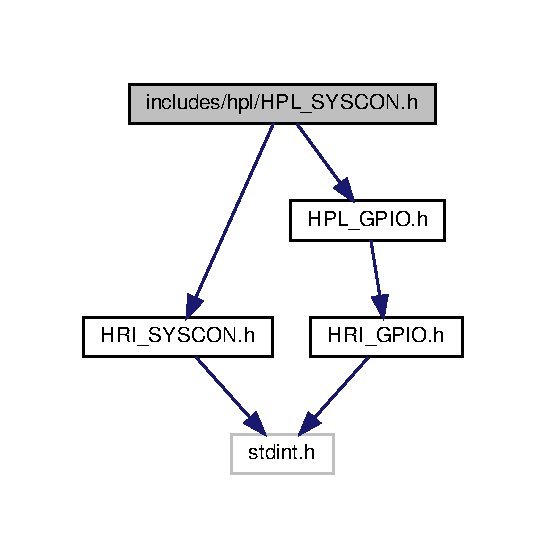
\includegraphics[width=262pt]{d6/d7d/HPL__SYSCON_8h__incl}
\end{center}
\end{figure}
Gráfico de los archivos que directa o indirectamente incluyen a este archivo\+:\nopagebreak
\begin{figure}[H]
\begin{center}
\leavevmode
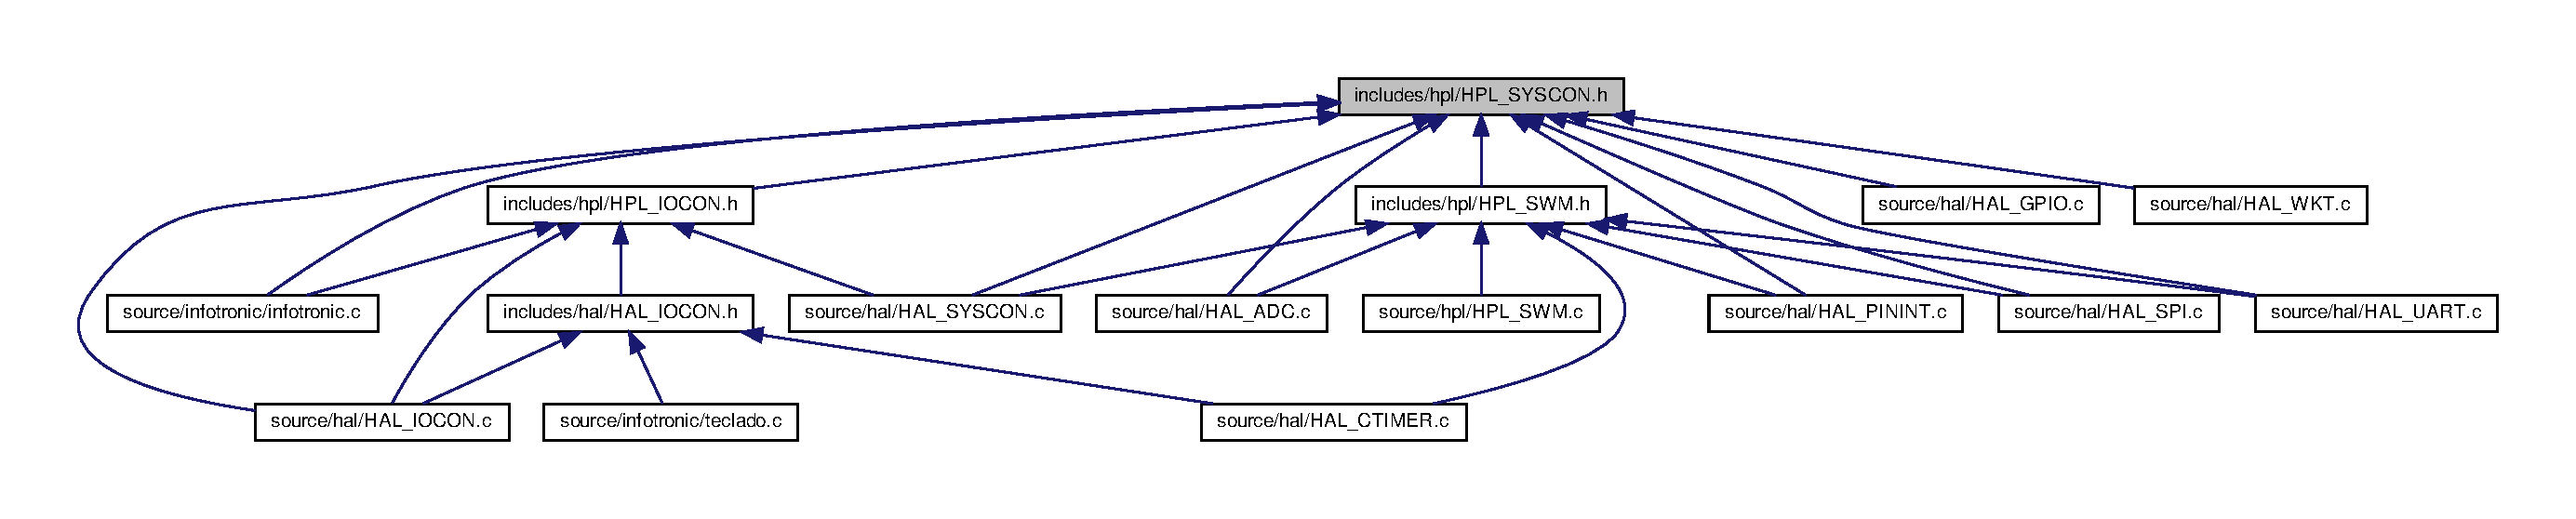
\includegraphics[width=350pt]{d3/d84/HPL__SYSCON_8h__dep__incl}
\end{center}
\end{figure}
\subsection*{Enumeraciones}
\begin{DoxyCompactItemize}
\item 
\mbox{\Hypertarget{HPL__SYSCON_8h_a7a694b3c9ecc3cd13a0e9341e60c8e17}\label{HPL__SYSCON_8h_a7a694b3c9ecc3cd13a0e9341e60c8e17}} 
enum {\bfseries S\+Y\+S\+C\+O\+N\+\_\+bypass\+\_\+sel\+\_\+en} \{ {\bfseries S\+Y\+S\+C\+O\+N\+\_\+\+B\+Y\+P\+A\+S\+S\+\_\+\+D\+I\+S\+A\+B\+L\+ED} = 0, 
{\bfseries S\+Y\+S\+C\+O\+N\+\_\+\+B\+Y\+P\+A\+S\+S\+\_\+\+E\+N\+A\+B\+L\+ED}
 \}
\item 
\mbox{\Hypertarget{HPL__SYSCON_8h_ac372d5894dafb0ccd348a6dd708bdd79}\label{HPL__SYSCON_8h_ac372d5894dafb0ccd348a6dd708bdd79}} 
enum {\bfseries S\+Y\+S\+C\+O\+N\+\_\+freqrange\+\_\+sel\+\_\+en} \{ {\bfseries S\+Y\+S\+C\+O\+N\+\_\+\+F\+R\+E\+Q\+R\+A\+N\+G\+E\+\_\+\+M\+I\+N\+U\+S\+\_\+20\+M\+HZ} = 0, 
{\bfseries S\+Y\+S\+C\+O\+N\+\_\+\+F\+R\+E\+Q\+R\+A\+N\+G\+E\+\_\+\+P\+L\+U\+S\+\_\+20\+M\+HZ}
 \}
\item 
\mbox{\Hypertarget{HPL__SYSCON_8h_abdafa5df63e4a2885b3dbdd8d56eabf1}\label{HPL__SYSCON_8h_abdafa5df63e4a2885b3dbdd8d56eabf1}} 
enum {\bfseries S\+Y\+S\+C\+O\+N\+\_\+watchdog\+\_\+clkana\+\_\+sel\+\_\+en} \{ \newline
{\bfseries S\+Y\+S\+C\+O\+N\+\_\+\+W\+A\+T\+C\+H\+D\+O\+G\+\_\+\+C\+L\+K\+A\+N\+A\+\_\+0\+K\+HZ} = 0, 
{\bfseries S\+Y\+S\+C\+O\+N\+\_\+\+W\+A\+T\+C\+H\+D\+O\+G\+\_\+\+C\+L\+K\+A\+N\+A\+\_\+600\+K\+HZ}, 
{\bfseries S\+Y\+S\+C\+O\+N\+\_\+\+W\+A\+T\+C\+H\+D\+O\+G\+\_\+\+C\+L\+K\+A\+N\+A\+\_\+1050\+K\+HZ}, 
{\bfseries S\+Y\+S\+C\+O\+N\+\_\+\+W\+A\+T\+C\+H\+D\+O\+G\+\_\+\+C\+L\+K\+A\+N\+A\+\_\+1400\+K\+HZ}, 
\newline
{\bfseries S\+Y\+S\+C\+O\+N\+\_\+\+W\+A\+T\+C\+H\+D\+O\+G\+\_\+\+C\+L\+K\+A\+N\+A\+\_\+1750\+K\+HZ}, 
{\bfseries S\+Y\+S\+C\+O\+N\+\_\+\+W\+A\+T\+C\+H\+D\+O\+G\+\_\+\+C\+L\+K\+A\+N\+A\+\_\+2100\+K\+HZ}, 
{\bfseries S\+Y\+S\+C\+O\+N\+\_\+\+W\+A\+T\+C\+H\+D\+O\+G\+\_\+\+C\+L\+K\+A\+N\+A\+\_\+2400\+K\+HZ}, 
{\bfseries S\+Y\+S\+C\+O\+N\+\_\+\+W\+A\+T\+C\+H\+D\+O\+G\+\_\+\+C\+L\+K\+A\+N\+A\+\_\+3000\+K\+HZ}, 
\newline
{\bfseries S\+Y\+S\+C\+O\+N\+\_\+\+W\+A\+T\+C\+H\+D\+O\+G\+\_\+\+C\+L\+K\+A\+N\+A\+\_\+3250\+K\+HZ}, 
{\bfseries S\+Y\+S\+C\+O\+N\+\_\+\+W\+A\+T\+C\+H\+D\+O\+G\+\_\+\+C\+L\+K\+A\+N\+A\+\_\+3500\+K\+HZ}, 
{\bfseries S\+Y\+S\+C\+O\+N\+\_\+\+W\+A\+T\+C\+H\+D\+O\+G\+\_\+\+C\+L\+K\+A\+N\+A\+\_\+3750\+K\+HZ}, 
{\bfseries S\+Y\+S\+C\+O\+N\+\_\+\+W\+A\+T\+C\+H\+D\+O\+G\+\_\+\+C\+L\+K\+A\+N\+A\+\_\+4000\+K\+HZ}, 
\newline
{\bfseries S\+Y\+S\+C\+O\+N\+\_\+\+W\+A\+T\+C\+H\+D\+O\+G\+\_\+\+C\+L\+K\+A\+N\+A\+\_\+4200\+K\+HZ}, 
{\bfseries S\+Y\+S\+C\+O\+N\+\_\+\+W\+A\+T\+C\+H\+D\+O\+G\+\_\+\+C\+L\+K\+A\+N\+A\+\_\+4400\+K\+HZ}, 
{\bfseries S\+Y\+S\+C\+O\+N\+\_\+\+W\+A\+T\+C\+H\+D\+O\+G\+\_\+\+C\+L\+K\+A\+N\+A\+\_\+4600\+K\+HZ}
 \}
\item 
\mbox{\Hypertarget{HPL__SYSCON_8h_a3dd8b9107f51aba2bfbfb20991df33c2}\label{HPL__SYSCON_8h_a3dd8b9107f51aba2bfbfb20991df33c2}} 
enum {\bfseries S\+Y\+S\+C\+O\+N\+\_\+pll\+\_\+source\+\_\+sel\+\_\+en} \{ {\bfseries S\+Y\+S\+C\+O\+N\+\_\+\+P\+L\+L\+\_\+\+S\+O\+U\+R\+C\+E\+\_\+\+S\+E\+L\+\_\+\+F\+RO} = 0, 
{\bfseries S\+Y\+S\+C\+O\+N\+\_\+\+P\+L\+L\+\_\+\+S\+O\+U\+R\+C\+E\+\_\+\+S\+E\+L\+\_\+\+E\+X\+T\+\_\+\+C\+LK}, 
{\bfseries S\+Y\+S\+C\+O\+N\+\_\+\+P\+L\+L\+\_\+\+S\+O\+U\+R\+C\+E\+\_\+\+S\+E\+L\+\_\+\+W\+A\+T\+C\+H\+D\+OG}, 
{\bfseries S\+Y\+S\+C\+O\+N\+\_\+\+P\+L\+L\+\_\+\+S\+O\+U\+R\+C\+E\+\_\+\+S\+E\+L\+\_\+\+F\+R\+O\+\_\+\+D\+IV}
 \}
\item 
\mbox{\Hypertarget{HPL__SYSCON_8h_a309fc9d4d2661a6d55a21b8a25df4e45}\label{HPL__SYSCON_8h_a309fc9d4d2661a6d55a21b8a25df4e45}} 
enum {\bfseries S\+Y\+S\+C\+O\+N\+\_\+main\+\_\+clock\+\_\+sel\+\_\+en} \{ \newline
{\bfseries S\+Y\+S\+C\+O\+N\+\_\+\+M\+A\+I\+N\+\_\+\+C\+L\+O\+C\+K\+\_\+\+S\+E\+L\+\_\+\+F\+RO} = 0, 
{\bfseries S\+Y\+S\+C\+O\+N\+\_\+\+M\+A\+I\+N\+\_\+\+C\+L\+O\+C\+K\+\_\+\+S\+E\+L\+\_\+\+E\+X\+T\+\_\+\+C\+LK}, 
{\bfseries S\+Y\+S\+C\+O\+N\+\_\+\+M\+A\+I\+N\+\_\+\+C\+L\+O\+C\+K\+\_\+\+S\+E\+L\+\_\+\+W\+A\+T\+C\+H\+D\+OG}, 
{\bfseries S\+Y\+S\+C\+O\+N\+\_\+\+M\+A\+I\+N\+\_\+\+C\+L\+O\+C\+K\+\_\+\+S\+E\+L\+\_\+\+F\+R\+O\+\_\+\+D\+IV}, 
\newline
{\bfseries S\+Y\+S\+C\+O\+N\+\_\+\+M\+A\+I\+N\+\_\+\+C\+L\+O\+C\+K\+\_\+\+S\+E\+L\+\_\+\+P\+LL}
 \}
\item 
\mbox{\Hypertarget{HPL__SYSCON_8h_a96be9e6cfdc3169ded398c42c1feb495}\label{HPL__SYSCON_8h_a96be9e6cfdc3169ded398c42c1feb495}} 
enum {\bfseries S\+Y\+S\+C\+O\+N\+\_\+capacitive\+\_\+clock\+\_\+sel\+\_\+en} \{ \newline
{\bfseries S\+Y\+S\+C\+O\+N\+\_\+\+C\+A\+P\+A\+C\+I\+T\+I\+V\+E\+\_\+\+C\+L\+O\+C\+K\+\_\+\+S\+E\+L\+\_\+\+F\+RO} = 0, 
{\bfseries S\+Y\+S\+C\+O\+N\+\_\+\+C\+A\+P\+A\+C\+I\+T\+I\+V\+E\+\_\+\+C\+L\+O\+C\+K\+\_\+\+S\+E\+L\+\_\+\+M\+A\+I\+N\+\_\+\+C\+L\+O\+CK}, 
{\bfseries S\+Y\+S\+C\+O\+N\+\_\+\+C\+A\+P\+A\+C\+I\+T\+I\+V\+E\+\_\+\+C\+L\+O\+C\+K\+\_\+\+S\+E\+L\+\_\+\+S\+Y\+S\+\_\+\+P\+LL}, 
{\bfseries S\+Y\+S\+C\+O\+N\+\_\+\+C\+A\+P\+A\+C\+I\+T\+I\+V\+E\+\_\+\+C\+L\+O\+C\+K\+\_\+\+S\+E\+L\+\_\+\+F\+R\+O\+\_\+\+D\+IV}, 
\newline
{\bfseries S\+Y\+S\+C\+O\+N\+\_\+\+C\+A\+P\+A\+C\+I\+T\+I\+V\+E\+\_\+\+C\+L\+O\+C\+K\+\_\+\+S\+E\+L\+\_\+\+W\+A\+T\+C\+H\+D\+O\+G\+\_\+\+O\+SC}
 \}
\item 
\mbox{\Hypertarget{HPL__SYSCON_8h_ad25d1973ac386c4b5f0c74faff9331f2}\label{HPL__SYSCON_8h_ad25d1973ac386c4b5f0c74faff9331f2}} 
enum {\bfseries S\+Y\+S\+C\+O\+N\+\_\+adc\+\_\+clock\+\_\+sel\+\_\+en} \{ {\bfseries S\+Y\+S\+C\+O\+N\+\_\+\+A\+D\+C\+\_\+\+C\+L\+O\+C\+K\+\_\+\+S\+E\+L\+\_\+\+F\+RO} = 0, 
{\bfseries S\+Y\+S\+C\+O\+N\+\_\+\+A\+D\+C\+\_\+\+C\+L\+O\+C\+K\+\_\+\+S\+E\+L\+\_\+\+S\+Y\+S\+\_\+\+P\+LL}
 \}
\item 
\mbox{\Hypertarget{HPL__SYSCON_8h_a39f44c3ca43e77c52756da1c18ecd693}\label{HPL__SYSCON_8h_a39f44c3ca43e77c52756da1c18ecd693}} 
enum {\bfseries S\+Y\+S\+C\+O\+N\+\_\+sct\+\_\+clock\+\_\+sel\+\_\+en} \{ {\bfseries S\+Y\+S\+C\+O\+N\+\_\+\+S\+C\+T\+\_\+\+C\+L\+O\+C\+K\+\_\+\+S\+E\+L\+\_\+\+F\+RO} = 0, 
{\bfseries S\+Y\+S\+C\+O\+N\+\_\+\+S\+C\+T\+\_\+\+C\+L\+O\+C\+K\+\_\+\+S\+E\+L\+\_\+\+M\+A\+I\+N\+\_\+\+C\+L\+O\+CK}, 
{\bfseries S\+Y\+S\+C\+O\+N\+\_\+\+S\+C\+T\+\_\+\+C\+L\+O\+C\+K\+\_\+\+S\+E\+L\+\_\+\+S\+Y\+S\+\_\+\+P\+LL}
 \}
\item 
\mbox{\Hypertarget{HPL__SYSCON_8h_aa5a662a8047708f6fa4a97ad8afd3581}\label{HPL__SYSCON_8h_aa5a662a8047708f6fa4a97ad8afd3581}} 
enum {\bfseries S\+Y\+S\+C\+O\+N\+\_\+ext\+\_\+clock\+\_\+source\+\_\+sel\+\_\+en} \{ {\bfseries S\+Y\+S\+C\+O\+N\+\_\+\+E\+X\+T\+\_\+\+C\+L\+O\+C\+K\+\_\+\+S\+O\+U\+R\+C\+E\+\_\+\+S\+E\+L\+\_\+\+C\+R\+Y\+S\+T\+AL} = 0, 
{\bfseries S\+Y\+S\+C\+O\+N\+\_\+\+E\+X\+T\+\_\+\+C\+L\+O\+C\+K\+\_\+\+S\+O\+U\+R\+C\+E\+\_\+\+S\+E\+L\+\_\+\+C\+L\+K\+\_\+\+IN}
 \}
\item 
\mbox{\Hypertarget{HPL__SYSCON_8h_a2096d496a1cf74044c97170c1bf77b07}\label{HPL__SYSCON_8h_a2096d496a1cf74044c97170c1bf77b07}} 
enum {\bfseries S\+Y\+S\+C\+O\+N\+\_\+enable\+\_\+clock\+\_\+sel\+\_\+en} \{ \newline
{\bfseries S\+Y\+S\+C\+O\+N\+\_\+\+E\+N\+A\+B\+L\+E\+\_\+\+C\+L\+O\+C\+K\+\_\+\+S\+E\+L\+\_\+\+R\+OM} = 1, 
{\bfseries S\+Y\+S\+C\+O\+N\+\_\+\+E\+N\+A\+B\+L\+E\+\_\+\+C\+L\+O\+C\+K\+\_\+\+S\+E\+L\+\_\+\+R\+AM}, 
{\bfseries S\+Y\+S\+C\+O\+N\+\_\+\+E\+N\+A\+B\+L\+E\+\_\+\+C\+L\+O\+C\+K\+\_\+\+S\+E\+L\+\_\+\+F\+L\+A\+SH} = 4, 
{\bfseries S\+Y\+S\+C\+O\+N\+\_\+\+E\+N\+A\+B\+L\+E\+\_\+\+C\+L\+O\+C\+K\+\_\+\+S\+E\+L\+\_\+\+I\+I\+C0}, 
\newline
{\bfseries S\+Y\+S\+C\+O\+N\+\_\+\+E\+N\+A\+B\+L\+E\+\_\+\+C\+L\+O\+C\+K\+\_\+\+S\+E\+L\+\_\+\+G\+P\+I\+O0}, 
{\bfseries S\+Y\+S\+C\+O\+N\+\_\+\+E\+N\+A\+B\+L\+E\+\_\+\+C\+L\+O\+C\+K\+\_\+\+S\+E\+L\+\_\+\+S\+WM}, 
{\bfseries S\+Y\+S\+C\+O\+N\+\_\+\+E\+N\+A\+B\+L\+E\+\_\+\+C\+L\+O\+C\+K\+\_\+\+S\+E\+L\+\_\+\+S\+CT}, 
{\bfseries S\+Y\+S\+C\+O\+N\+\_\+\+E\+N\+A\+B\+L\+E\+\_\+\+C\+L\+O\+C\+K\+\_\+\+S\+E\+L\+\_\+\+W\+KT}, 
\newline
{\bfseries S\+Y\+S\+C\+O\+N\+\_\+\+E\+N\+A\+B\+L\+E\+\_\+\+C\+L\+O\+C\+K\+\_\+\+S\+E\+L\+\_\+\+M\+RT}, 
{\bfseries S\+Y\+S\+C\+O\+N\+\_\+\+E\+N\+A\+B\+L\+E\+\_\+\+C\+L\+O\+C\+K\+\_\+\+S\+E\+L\+\_\+\+S\+P\+I0}, 
{\bfseries S\+Y\+S\+C\+O\+N\+\_\+\+E\+N\+A\+B\+L\+E\+\_\+\+C\+L\+O\+C\+K\+\_\+\+S\+E\+L\+\_\+\+S\+P\+I1}, 
{\bfseries S\+Y\+S\+C\+O\+N\+\_\+\+E\+N\+A\+B\+L\+E\+\_\+\+C\+L\+O\+C\+K\+\_\+\+S\+E\+L\+\_\+\+C\+RC}, 
\newline
{\bfseries S\+Y\+S\+C\+O\+N\+\_\+\+E\+N\+A\+B\+L\+E\+\_\+\+C\+L\+O\+C\+K\+\_\+\+S\+E\+L\+\_\+\+U\+A\+R\+T0}, 
{\bfseries S\+Y\+S\+C\+O\+N\+\_\+\+E\+N\+A\+B\+L\+E\+\_\+\+C\+L\+O\+C\+K\+\_\+\+S\+E\+L\+\_\+\+U\+A\+R\+T1}, 
{\bfseries S\+Y\+S\+C\+O\+N\+\_\+\+E\+N\+A\+B\+L\+E\+\_\+\+C\+L\+O\+C\+K\+\_\+\+S\+E\+L\+\_\+\+U\+A\+R\+T2}, 
{\bfseries S\+Y\+S\+C\+O\+N\+\_\+\+E\+N\+A\+B\+L\+E\+\_\+\+C\+L\+O\+C\+K\+\_\+\+S\+E\+L\+\_\+\+W\+W\+DT}, 
\newline
{\bfseries S\+Y\+S\+C\+O\+N\+\_\+\+E\+N\+A\+B\+L\+E\+\_\+\+C\+L\+O\+C\+K\+\_\+\+S\+E\+L\+\_\+\+I\+O\+C\+ON}, 
{\bfseries S\+Y\+S\+C\+O\+N\+\_\+\+E\+N\+A\+B\+L\+E\+\_\+\+C\+L\+O\+C\+K\+\_\+\+S\+E\+L\+\_\+\+A\+C\+MP}, 
{\bfseries S\+Y\+S\+C\+O\+N\+\_\+\+E\+N\+A\+B\+L\+E\+\_\+\+C\+L\+O\+C\+K\+\_\+\+S\+E\+L\+\_\+\+G\+P\+I\+O1}, 
{\bfseries S\+Y\+S\+C\+O\+N\+\_\+\+E\+N\+A\+B\+L\+E\+\_\+\+C\+L\+O\+C\+K\+\_\+\+S\+E\+L\+\_\+\+I\+I\+C1}, 
\newline
{\bfseries S\+Y\+S\+C\+O\+N\+\_\+\+E\+N\+A\+B\+L\+E\+\_\+\+C\+L\+O\+C\+K\+\_\+\+S\+E\+L\+\_\+\+I\+I\+C2}, 
{\bfseries S\+Y\+S\+C\+O\+N\+\_\+\+E\+N\+A\+B\+L\+E\+\_\+\+C\+L\+O\+C\+K\+\_\+\+S\+E\+L\+\_\+\+I\+I\+C3}, 
{\bfseries S\+Y\+S\+C\+O\+N\+\_\+\+E\+N\+A\+B\+L\+E\+\_\+\+C\+L\+O\+C\+K\+\_\+\+S\+E\+L\+\_\+\+A\+DC}, 
{\bfseries S\+Y\+S\+C\+O\+N\+\_\+\+E\+N\+A\+B\+L\+E\+\_\+\+C\+L\+O\+C\+K\+\_\+\+S\+E\+L\+\_\+\+C\+T\+I\+M\+ER}, 
\newline
{\bfseries S\+Y\+S\+C\+O\+N\+\_\+\+E\+N\+A\+B\+L\+E\+\_\+\+C\+L\+O\+C\+K\+\_\+\+S\+E\+L\+\_\+\+M\+TB}, 
{\bfseries S\+Y\+S\+C\+O\+N\+\_\+\+E\+N\+A\+B\+L\+E\+\_\+\+C\+L\+O\+C\+K\+\_\+\+S\+E\+L\+\_\+\+D\+A\+C0}, 
{\bfseries S\+Y\+S\+C\+O\+N\+\_\+\+E\+N\+A\+B\+L\+E\+\_\+\+C\+L\+O\+C\+K\+\_\+\+S\+E\+L\+\_\+\+G\+P\+I\+O\+\_\+\+I\+NT}, 
{\bfseries S\+Y\+S\+C\+O\+N\+\_\+\+E\+N\+A\+B\+L\+E\+\_\+\+C\+L\+O\+C\+K\+\_\+\+S\+E\+L\+\_\+\+D\+MA}, 
\newline
{\bfseries S\+Y\+S\+C\+O\+N\+\_\+\+E\+N\+A\+B\+L\+E\+\_\+\+C\+L\+O\+C\+K\+\_\+\+S\+E\+L\+\_\+\+U\+A\+R\+T3}, 
{\bfseries S\+Y\+S\+C\+O\+N\+\_\+\+E\+N\+A\+B\+L\+E\+\_\+\+C\+L\+O\+C\+K\+\_\+\+S\+E\+L\+\_\+\+U\+A\+R\+T4}, 
{\bfseries S\+Y\+S\+C\+O\+N\+\_\+\+E\+N\+A\+B\+L\+E\+\_\+\+C\+L\+O\+C\+K\+\_\+\+S\+E\+L\+\_\+\+C\+A\+PT}, 
{\bfseries S\+Y\+S\+C\+O\+N\+\_\+\+E\+N\+A\+B\+L\+E\+\_\+\+C\+L\+O\+C\+K\+\_\+\+S\+E\+L\+\_\+\+D\+A\+C1}
 \}
\item 
\mbox{\Hypertarget{HPL__SYSCON_8h_ab112f30c86d0a96de715aec515ad9cc7}\label{HPL__SYSCON_8h_ab112f30c86d0a96de715aec515ad9cc7}} 
enum {\bfseries S\+Y\+S\+C\+O\+N\+\_\+reset\+\_\+sel\+\_\+en} \{ \newline
{\bfseries S\+Y\+S\+C\+O\+N\+\_\+\+R\+E\+S\+E\+T\+\_\+\+S\+E\+L\+\_\+\+F\+L\+A\+SH} = 4, 
{\bfseries S\+Y\+S\+C\+O\+N\+\_\+\+R\+E\+S\+E\+T\+\_\+\+S\+E\+L\+\_\+\+I\+I\+C0}, 
{\bfseries S\+Y\+S\+C\+O\+N\+\_\+\+R\+E\+S\+E\+T\+\_\+\+S\+E\+L\+\_\+\+G\+P\+I\+O0}, 
{\bfseries S\+Y\+S\+C\+O\+N\+\_\+\+R\+E\+S\+E\+T\+\_\+\+S\+E\+L\+\_\+\+S\+WM}, 
\newline
{\bfseries S\+Y\+S\+C\+O\+N\+\_\+\+R\+E\+S\+E\+T\+\_\+\+S\+E\+L\+\_\+\+S\+CT}, 
{\bfseries S\+Y\+S\+C\+O\+N\+\_\+\+R\+E\+S\+E\+T\+\_\+\+S\+E\+L\+\_\+\+W\+KT}, 
{\bfseries S\+Y\+S\+C\+O\+N\+\_\+\+R\+E\+S\+E\+T\+\_\+\+S\+E\+L\+\_\+\+M\+RT}, 
{\bfseries S\+Y\+S\+C\+O\+N\+\_\+\+R\+E\+S\+E\+T\+\_\+\+S\+E\+L\+\_\+\+S\+P\+I0}, 
\newline
{\bfseries S\+Y\+S\+C\+O\+N\+\_\+\+R\+E\+S\+E\+T\+\_\+\+S\+E\+L\+\_\+\+S\+P\+I1}, 
{\bfseries S\+Y\+S\+C\+O\+N\+\_\+\+R\+E\+S\+E\+T\+\_\+\+S\+E\+L\+\_\+\+C\+RC}, 
{\bfseries S\+Y\+S\+C\+O\+N\+\_\+\+R\+E\+S\+E\+T\+\_\+\+S\+E\+L\+\_\+\+U\+A\+R\+T0}, 
{\bfseries S\+Y\+S\+C\+O\+N\+\_\+\+R\+E\+S\+E\+T\+\_\+\+S\+E\+L\+\_\+\+U\+A\+R\+T1}, 
\newline
{\bfseries S\+Y\+S\+C\+O\+N\+\_\+\+R\+E\+S\+E\+T\+\_\+\+S\+E\+L\+\_\+\+U\+A\+R\+T2}, 
{\bfseries S\+Y\+S\+C\+O\+N\+\_\+\+R\+E\+S\+E\+T\+\_\+\+S\+E\+L\+\_\+\+I\+O\+C\+ON} = 18, 
{\bfseries S\+Y\+S\+C\+O\+N\+\_\+\+R\+E\+S\+E\+T\+\_\+\+S\+E\+L\+\_\+\+A\+C\+MP}, 
{\bfseries S\+Y\+S\+C\+O\+N\+\_\+\+R\+E\+S\+E\+T\+\_\+\+S\+E\+L\+\_\+\+G\+P\+I\+O1}, 
\newline
{\bfseries S\+Y\+S\+C\+O\+N\+\_\+\+R\+E\+S\+E\+T\+\_\+\+S\+E\+L\+\_\+\+I\+I\+C1}, 
{\bfseries S\+Y\+S\+C\+O\+N\+\_\+\+R\+E\+S\+E\+T\+\_\+\+S\+E\+L\+\_\+\+I\+I\+C2}, 
{\bfseries S\+Y\+S\+C\+O\+N\+\_\+\+R\+E\+S\+E\+T\+\_\+\+S\+E\+L\+\_\+\+I\+I\+C3}, 
{\bfseries S\+Y\+S\+C\+O\+N\+\_\+\+R\+E\+S\+E\+T\+\_\+\+S\+E\+L\+\_\+\+A\+DC}, 
\newline
{\bfseries S\+Y\+S\+C\+O\+N\+\_\+\+R\+E\+S\+E\+T\+\_\+\+S\+E\+L\+\_\+\+C\+T\+I\+M\+ER}, 
{\bfseries S\+Y\+S\+C\+O\+N\+\_\+\+R\+E\+S\+E\+T\+\_\+\+S\+E\+L\+\_\+\+D\+A\+C0} = 27, 
{\bfseries S\+Y\+S\+C\+O\+N\+\_\+\+R\+E\+S\+E\+T\+\_\+\+S\+E\+L\+\_\+\+G\+P\+I\+O\+I\+NT}, 
{\bfseries S\+Y\+S\+C\+O\+N\+\_\+\+R\+E\+S\+E\+T\+\_\+\+S\+E\+L\+\_\+\+D\+MA}, 
\newline
{\bfseries S\+Y\+S\+C\+O\+N\+\_\+\+R\+E\+S\+E\+T\+\_\+\+S\+E\+L\+\_\+\+U\+A\+R\+T3}, 
{\bfseries S\+Y\+S\+C\+O\+N\+\_\+\+R\+E\+S\+E\+T\+\_\+\+S\+E\+L\+\_\+\+U\+A\+R\+T4}, 
{\bfseries S\+Y\+S\+C\+O\+N\+\_\+\+R\+E\+S\+E\+T\+\_\+\+S\+E\+L\+\_\+\+C\+A\+PT}, 
{\bfseries S\+Y\+S\+C\+O\+N\+\_\+\+R\+E\+S\+E\+T\+\_\+\+S\+E\+L\+\_\+\+D\+A\+C1}, 
\newline
{\bfseries S\+Y\+S\+C\+O\+N\+\_\+\+R\+E\+S\+E\+T\+\_\+\+S\+E\+L\+\_\+\+F\+R\+G0} = 35, 
{\bfseries S\+Y\+S\+C\+O\+N\+\_\+\+R\+E\+S\+E\+T\+\_\+\+S\+E\+L\+\_\+\+F\+R\+G1}
 \}
\item 
\mbox{\Hypertarget{HPL__SYSCON_8h_a5b7c97573f9e976e4bb5bddf20bb4688}\label{HPL__SYSCON_8h_a5b7c97573f9e976e4bb5bddf20bb4688}} 
enum {\bfseries S\+Y\+S\+C\+O\+N\+\_\+peripheral\+\_\+sel\+\_\+en} \{ \newline
{\bfseries S\+Y\+S\+C\+O\+N\+\_\+\+P\+E\+R\+I\+P\+H\+E\+R\+A\+L\+\_\+\+S\+E\+L\+\_\+\+U\+A\+R\+T0} = 0, 
{\bfseries S\+Y\+S\+C\+O\+N\+\_\+\+P\+E\+R\+I\+P\+H\+E\+R\+A\+L\+\_\+\+S\+E\+L\+\_\+\+U\+A\+R\+T1}, 
{\bfseries S\+Y\+S\+C\+O\+N\+\_\+\+P\+E\+R\+I\+P\+H\+E\+R\+A\+L\+\_\+\+S\+E\+L\+\_\+\+U\+A\+R\+T2}, 
{\bfseries S\+Y\+S\+C\+O\+N\+\_\+\+P\+E\+R\+I\+P\+H\+E\+R\+A\+L\+\_\+\+S\+E\+L\+\_\+\+U\+A\+R\+T3}, 
\newline
{\bfseries S\+Y\+S\+C\+O\+N\+\_\+\+P\+E\+R\+I\+P\+H\+E\+R\+A\+L\+\_\+\+S\+E\+L\+\_\+\+U\+A\+R\+T4}, 
{\bfseries S\+Y\+S\+C\+O\+N\+\_\+\+P\+E\+R\+I\+P\+H\+E\+R\+A\+L\+\_\+\+S\+E\+L\+\_\+\+I2\+C0}, 
{\bfseries S\+Y\+S\+C\+O\+N\+\_\+\+P\+E\+R\+I\+P\+H\+E\+R\+A\+L\+\_\+\+S\+E\+L\+\_\+\+I2\+C1}, 
{\bfseries S\+Y\+S\+C\+O\+N\+\_\+\+P\+E\+R\+I\+P\+H\+E\+R\+A\+L\+\_\+\+S\+E\+L\+\_\+\+I2\+C2}, 
\newline
{\bfseries S\+Y\+S\+C\+O\+N\+\_\+\+P\+E\+R\+I\+P\+H\+E\+R\+A\+L\+\_\+\+S\+E\+L\+\_\+\+I2\+C3}, 
{\bfseries S\+Y\+S\+C\+O\+N\+\_\+\+P\+E\+R\+I\+P\+H\+E\+R\+A\+L\+\_\+\+S\+E\+L\+\_\+\+S\+P\+I0}, 
{\bfseries S\+Y\+S\+C\+O\+N\+\_\+\+P\+E\+R\+I\+P\+H\+E\+R\+A\+L\+\_\+\+S\+E\+L\+\_\+\+S\+P\+I1}
 \}
\item 
\mbox{\Hypertarget{HPL__SYSCON_8h_ac5d228c67b914f93912d601b7735ec6e}\label{HPL__SYSCON_8h_ac5d228c67b914f93912d601b7735ec6e}} 
enum {\bfseries S\+Y\+S\+C\+O\+N\+\_\+peripheral\+\_\+clock\+\_\+sel\+\_\+en} \{ \newline
{\bfseries S\+Y\+S\+C\+O\+N\+\_\+\+P\+E\+R\+I\+P\+H\+E\+R\+A\+L\+\_\+\+C\+L\+O\+C\+K\+\_\+\+S\+E\+L\+\_\+\+F\+RO} = 0, 
{\bfseries S\+Y\+S\+C\+O\+N\+\_\+\+P\+E\+R\+I\+P\+H\+E\+R\+A\+L\+\_\+\+C\+L\+O\+C\+K\+\_\+\+S\+E\+L\+\_\+\+M\+A\+IN}, 
{\bfseries S\+Y\+S\+C\+O\+N\+\_\+\+P\+E\+R\+I\+P\+H\+E\+R\+A\+L\+\_\+\+C\+L\+O\+C\+K\+\_\+\+S\+E\+L\+\_\+\+F\+R\+G0}, 
{\bfseries S\+Y\+S\+C\+O\+N\+\_\+\+P\+E\+R\+I\+P\+H\+E\+R\+A\+L\+\_\+\+C\+L\+O\+C\+K\+\_\+\+S\+E\+L\+\_\+\+F\+R\+G1}, 
\newline
{\bfseries S\+Y\+S\+C\+O\+N\+\_\+\+P\+E\+R\+I\+P\+H\+E\+R\+A\+L\+\_\+\+C\+L\+O\+C\+K\+\_\+\+S\+E\+L\+\_\+\+F\+R\+O\+\_\+\+D\+IV}, 
{\bfseries S\+Y\+S\+C\+O\+N\+\_\+\+P\+E\+R\+I\+P\+H\+E\+R\+A\+L\+\_\+\+C\+L\+O\+C\+K\+\_\+\+S\+E\+L\+\_\+\+N\+O\+NE} = 7
 \}
\item 
\mbox{\Hypertarget{HPL__SYSCON_8h_a07f2dc9916dbd8835f2e5f81507e7f2b}\label{HPL__SYSCON_8h_a07f2dc9916dbd8835f2e5f81507e7f2b}} 
enum {\bfseries S\+Y\+S\+C\+O\+N\+\_\+frg\+\_\+clock\+\_\+sel\+\_\+en} \{ {\bfseries S\+Y\+S\+C\+O\+N\+\_\+\+F\+R\+G\+\_\+\+C\+L\+O\+C\+K\+\_\+\+S\+E\+L\+\_\+\+F\+RO} = 0, 
{\bfseries S\+Y\+S\+C\+O\+N\+\_\+\+F\+R\+G\+\_\+\+C\+L\+O\+C\+K\+\_\+\+S\+E\+L\+\_\+\+M\+A\+I\+N\+\_\+\+C\+L\+O\+CK}, 
{\bfseries S\+Y\+S\+C\+O\+N\+\_\+\+F\+R\+G\+\_\+\+C\+L\+O\+C\+K\+\_\+\+S\+E\+L\+\_\+\+S\+Y\+S\+\_\+\+P\+LL}, 
{\bfseries S\+Y\+S\+C\+O\+N\+\_\+\+F\+R\+G\+\_\+\+C\+L\+O\+C\+K\+\_\+\+S\+E\+L\+\_\+\+N\+O\+NE}
 \}
\item 
\mbox{\Hypertarget{HPL__SYSCON_8h_a24590b198c0c50184d3bf9c65f91491f}\label{HPL__SYSCON_8h_a24590b198c0c50184d3bf9c65f91491f}} 
enum {\bfseries S\+Y\+S\+C\+O\+N\+\_\+clkout\+\_\+source\+\_\+sel\+\_\+en} \{ \newline
{\bfseries S\+Y\+S\+C\+O\+N\+\_\+\+C\+L\+K\+O\+U\+T\+\_\+\+S\+O\+U\+R\+C\+E\+\_\+\+S\+E\+L\+\_\+\+F\+RO} = 0, 
{\bfseries S\+Y\+S\+C\+O\+N\+\_\+\+C\+L\+K\+O\+U\+T\+\_\+\+S\+O\+U\+R\+C\+E\+\_\+\+S\+E\+L\+\_\+\+M\+A\+I\+N\+\_\+\+C\+L\+O\+CK}, 
{\bfseries S\+Y\+S\+C\+O\+N\+\_\+\+C\+L\+K\+O\+U\+T\+\_\+\+S\+O\+U\+R\+C\+E\+\_\+\+S\+E\+L\+\_\+\+S\+Y\+S\+\_\+\+P\+LL}, 
{\bfseries S\+Y\+S\+C\+O\+N\+\_\+\+C\+L\+K\+O\+U\+T\+\_\+\+S\+O\+U\+R\+C\+E\+\_\+\+S\+E\+L\+\_\+\+E\+X\+T\+\_\+\+C\+L\+O\+CK}, 
\newline
{\bfseries S\+Y\+S\+C\+O\+N\+\_\+\+C\+L\+K\+O\+U\+T\+\_\+\+S\+O\+U\+R\+C\+E\+\_\+\+S\+E\+L\+\_\+\+W\+A\+T\+C\+H\+D\+O\+G\+\_\+\+O\+SC}
 \}
\item 
\mbox{\Hypertarget{HPL__SYSCON_8h_a5f3ab382e573cd575f2c22ff12bbe44d}\label{HPL__SYSCON_8h_a5f3ab382e573cd575f2c22ff12bbe44d}} 
enum {\bfseries S\+Y\+S\+C\+O\+N\+\_\+bod\+\_\+level\+\_\+en} \{ {\bfseries S\+Y\+S\+C\+O\+N\+\_\+\+B\+O\+D\+\_\+\+L\+E\+V\+E\+L\+\_\+1} = 1, 
{\bfseries S\+Y\+S\+C\+O\+N\+\_\+\+B\+O\+D\+\_\+\+L\+E\+V\+E\+L\+\_\+2}, 
{\bfseries S\+Y\+S\+C\+O\+N\+\_\+\+B\+O\+D\+\_\+\+L\+E\+V\+E\+L\+\_\+3}
 \}
\item 
\mbox{\Hypertarget{HPL__SYSCON_8h_ae4b4f7ada0fb530753613a5b4dcf1963}\label{HPL__SYSCON_8h_ae4b4f7ada0fb530753613a5b4dcf1963}} 
enum {\bfseries S\+Y\+S\+C\+O\+N\+\_\+bod\+\_\+enale\+\_\+en} \{ {\bfseries S\+Y\+S\+C\+O\+N\+\_\+\+B\+O\+D\+\_\+\+D\+I\+S\+A\+B\+LE} = 0, 
{\bfseries S\+Y\+S\+C\+O\+N\+\_\+\+B\+O\+D\+\_\+\+E\+N\+A\+B\+LE}
 \}
\item 
\mbox{\Hypertarget{HPL__SYSCON_8h_a488b5285ddf55eca6045664dffb0be98}\label{HPL__SYSCON_8h_a488b5285ddf55eca6045664dffb0be98}} 
enum {\bfseries S\+Y\+S\+C\+O\+N\+\_\+nmi\+\_\+enable\+\_\+en} \{ {\bfseries S\+Y\+S\+C\+O\+N\+\_\+\+N\+M\+I\+\_\+\+D\+I\+S\+A\+B\+LE} = 0, 
{\bfseries S\+Y\+S\+C\+O\+N\+\_\+\+N\+M\+I\+\_\+\+E\+N\+A\+B\+LE}
 \}
\item 
\mbox{\Hypertarget{HPL__SYSCON_8h_a749e07aa15b38515a27f40cc4ba37ade}\label{HPL__SYSCON_8h_a749e07aa15b38515a27f40cc4ba37ade}} 
enum {\bfseries S\+Y\+S\+C\+O\+N\+\_\+enable\+\_\+wakeup\+\_\+sel\+\_\+en} \{ \newline
{\bfseries S\+Y\+S\+C\+O\+N\+\_\+\+W\+A\+K\+E\+U\+P\+\_\+\+E\+N\+A\+B\+L\+E\+\_\+\+S\+E\+L\+\_\+\+P\+I\+N\+T0} = 0, 
{\bfseries S\+Y\+S\+C\+O\+N\+\_\+\+W\+A\+K\+E\+U\+P\+\_\+\+E\+N\+A\+B\+L\+E\+\_\+\+S\+E\+L\+\_\+\+P\+I\+N\+T1}, 
{\bfseries S\+Y\+S\+C\+O\+N\+\_\+\+W\+A\+K\+E\+U\+P\+\_\+\+E\+N\+A\+B\+L\+E\+\_\+\+S\+E\+L\+\_\+\+P\+I\+N\+T2}, 
{\bfseries S\+Y\+S\+C\+O\+N\+\_\+\+W\+A\+K\+E\+U\+P\+\_\+\+E\+N\+A\+B\+L\+E\+\_\+\+S\+E\+L\+\_\+\+P\+I\+N\+T3}, 
\newline
{\bfseries S\+Y\+S\+C\+O\+N\+\_\+\+W\+A\+K\+E\+U\+P\+\_\+\+E\+N\+A\+B\+L\+E\+\_\+\+S\+E\+L\+\_\+\+P\+I\+N\+T4}, 
{\bfseries S\+Y\+S\+C\+O\+N\+\_\+\+W\+A\+K\+E\+U\+P\+\_\+\+E\+N\+A\+B\+L\+E\+\_\+\+S\+E\+L\+\_\+\+P\+I\+N\+T5}, 
{\bfseries S\+Y\+S\+C\+O\+N\+\_\+\+W\+A\+K\+E\+U\+P\+\_\+\+E\+N\+A\+B\+L\+E\+\_\+\+S\+E\+L\+\_\+\+P\+I\+N\+T6}, 
{\bfseries S\+Y\+S\+C\+O\+N\+\_\+\+W\+A\+K\+E\+U\+P\+\_\+\+E\+N\+A\+B\+L\+E\+\_\+\+S\+E\+L\+\_\+\+P\+I\+N\+T7}, 
\newline
{\bfseries S\+Y\+S\+C\+O\+N\+\_\+\+W\+A\+K\+E\+U\+P\+\_\+\+E\+N\+A\+B\+L\+E\+\_\+\+S\+E\+L\+\_\+\+S\+P\+I0} = 32, 
{\bfseries S\+Y\+S\+C\+O\+N\+\_\+\+W\+A\+K\+E\+U\+P\+\_\+\+E\+N\+A\+B\+L\+E\+\_\+\+S\+E\+L\+\_\+\+S\+P\+I1}, 
{\bfseries S\+Y\+S\+C\+O\+N\+\_\+\+W\+A\+K\+E\+U\+P\+\_\+\+E\+N\+A\+B\+L\+E\+\_\+\+S\+E\+L\+\_\+\+U\+S\+A\+R\+T0} = 35, 
{\bfseries S\+Y\+S\+C\+O\+N\+\_\+\+W\+A\+K\+E\+U\+P\+\_\+\+E\+N\+A\+B\+L\+E\+\_\+\+S\+E\+L\+\_\+\+U\+S\+A\+R\+T1}, 
\newline
{\bfseries S\+Y\+S\+C\+O\+N\+\_\+\+W\+A\+K\+E\+U\+P\+\_\+\+E\+N\+A\+B\+L\+E\+\_\+\+S\+E\+L\+\_\+\+U\+S\+A\+R\+T2}, 
{\bfseries S\+Y\+S\+C\+O\+N\+\_\+\+W\+A\+K\+E\+U\+P\+\_\+\+E\+N\+A\+B\+L\+E\+\_\+\+S\+E\+L\+\_\+\+I\+I\+C1} = 39, 
{\bfseries S\+Y\+S\+C\+O\+N\+\_\+\+W\+A\+K\+E\+U\+P\+\_\+\+E\+N\+A\+B\+L\+E\+\_\+\+S\+E\+L\+\_\+\+I\+I\+C0}, 
{\bfseries S\+Y\+S\+C\+O\+N\+\_\+\+W\+A\+K\+E\+U\+P\+\_\+\+E\+N\+A\+B\+L\+E\+\_\+\+S\+E\+L\+\_\+\+C\+A\+P\+T\+O\+U\+CH} = 43, 
\newline
{\bfseries S\+Y\+S\+C\+O\+N\+\_\+\+W\+A\+K\+E\+U\+P\+\_\+\+E\+N\+A\+B\+L\+E\+\_\+\+S\+E\+L\+\_\+\+W\+W\+DT}, 
{\bfseries S\+Y\+S\+C\+O\+N\+\_\+\+W\+A\+K\+E\+U\+P\+\_\+\+E\+N\+A\+B\+L\+E\+\_\+\+S\+E\+L\+\_\+\+B\+OD}, 
{\bfseries S\+Y\+S\+C\+O\+N\+\_\+\+W\+A\+K\+E\+U\+P\+\_\+\+E\+N\+A\+B\+L\+E\+\_\+\+S\+E\+L\+\_\+\+W\+KT} = 47, 
{\bfseries S\+Y\+S\+C\+O\+N\+\_\+\+W\+A\+K\+E\+U\+P\+\_\+\+E\+N\+A\+B\+L\+E\+\_\+\+S\+E\+L\+\_\+\+I\+I\+C2} = 53, 
\newline
{\bfseries S\+Y\+S\+C\+O\+N\+\_\+\+W\+A\+K\+E\+U\+P\+\_\+\+E\+N\+A\+B\+L\+E\+\_\+\+S\+E\+L\+\_\+\+I\+I\+C3}, 
{\bfseries S\+Y\+S\+C\+O\+N\+\_\+\+W\+A\+K\+E\+U\+P\+\_\+\+E\+N\+A\+B\+L\+E\+\_\+\+S\+E\+L\+\_\+\+U\+S\+A\+R\+T3} = 62, 
{\bfseries S\+Y\+S\+C\+O\+N\+\_\+\+W\+A\+K\+E\+U\+P\+\_\+\+E\+N\+A\+B\+L\+E\+\_\+\+S\+E\+L\+\_\+\+U\+S\+A\+R\+T4}
 \}
\item 
\mbox{\Hypertarget{HPL__SYSCON_8h_a148798bf8134740c02689c944cd3e4c5}\label{HPL__SYSCON_8h_a148798bf8134740c02689c944cd3e4c5}} 
enum {\bfseries S\+Y\+S\+C\+O\+N\+\_\+deep\+\_\+sleep\+\_\+power\+\_\+en} \{ {\bfseries S\+Y\+S\+C\+O\+N\+\_\+\+D\+E\+E\+P\+\_\+\+S\+L\+E\+E\+P\+\_\+\+P\+O\+W\+E\+R\+ED} = 0, 
{\bfseries S\+Y\+S\+C\+O\+N\+\_\+\+D\+E\+E\+P\+\_\+\+S\+L\+E\+E\+P\+\_\+\+P\+O\+W\+E\+R\+E\+D\+\_\+\+D\+O\+WN}
 \}
\item 
\mbox{\Hypertarget{HPL__SYSCON_8h_a2c3bb00b1c2466c10670e2d0edb943fd}\label{HPL__SYSCON_8h_a2c3bb00b1c2466c10670e2d0edb943fd}} 
enum {\bfseries S\+Y\+S\+C\+O\+N\+\_\+wakeup\+\_\+power\+\_\+sel\+\_\+en} \{ \newline
{\bfseries S\+Y\+S\+C\+O\+N\+\_\+\+W\+A\+K\+E\+U\+P\+\_\+\+P\+O\+W\+E\+R\+\_\+\+S\+E\+L\+\_\+\+F\+R\+O\+O\+UT} = 0, 
{\bfseries S\+Y\+S\+C\+O\+N\+\_\+\+W\+A\+K\+E\+U\+P\+\_\+\+P\+O\+W\+E\+R\+\_\+\+S\+E\+L\+\_\+\+F\+RO}, 
{\bfseries S\+Y\+S\+C\+O\+N\+\_\+\+W\+A\+K\+E\+U\+P\+\_\+\+P\+O\+W\+E\+R\+\_\+\+S\+E\+L\+\_\+\+F\+L\+A\+SH}, 
{\bfseries S\+Y\+S\+C\+O\+N\+\_\+\+W\+A\+K\+E\+U\+P\+\_\+\+P\+O\+W\+E\+R\+\_\+\+S\+E\+L\+\_\+\+B\+OD}, 
\newline
{\bfseries S\+Y\+S\+C\+O\+N\+\_\+\+W\+A\+K\+E\+U\+P\+\_\+\+P\+O\+W\+E\+R\+\_\+\+S\+E\+L\+\_\+\+A\+DC}, 
{\bfseries S\+Y\+S\+C\+O\+N\+\_\+\+W\+A\+K\+E\+U\+P\+\_\+\+P\+O\+W\+E\+R\+\_\+\+S\+E\+L\+\_\+\+S\+Y\+S\+O\+SC}, 
{\bfseries S\+Y\+S\+C\+O\+N\+\_\+\+W\+A\+K\+E\+U\+P\+\_\+\+P\+O\+W\+E\+R\+\_\+\+S\+E\+L\+\_\+\+W\+D\+T\+O\+SC}, 
{\bfseries S\+Y\+S\+C\+O\+N\+\_\+\+W\+A\+K\+E\+U\+P\+\_\+\+P\+O\+W\+E\+R\+\_\+\+S\+E\+L\+\_\+\+S\+Y\+S\+P\+LL}, 
\newline
{\bfseries S\+Y\+S\+C\+O\+N\+\_\+\+W\+A\+K\+E\+U\+P\+\_\+\+P\+O\+W\+E\+R\+\_\+\+S\+E\+L\+\_\+\+V\+R\+E\+F2} = 10, 
{\bfseries S\+Y\+S\+C\+O\+N\+\_\+\+W\+A\+K\+E\+U\+P\+\_\+\+P\+O\+W\+E\+R\+\_\+\+S\+E\+L\+\_\+\+D\+A\+C0} = 13, 
{\bfseries S\+Y\+S\+C\+O\+N\+\_\+\+W\+A\+K\+E\+U\+P\+\_\+\+P\+O\+W\+E\+R\+\_\+\+S\+E\+L\+\_\+\+D\+A\+C1}, 
{\bfseries S\+Y\+S\+C\+O\+N\+\_\+\+W\+A\+K\+E\+U\+P\+\_\+\+P\+O\+W\+E\+R\+\_\+\+S\+E\+L\+\_\+\+A\+C\+MP}
 \}
\item 
\mbox{\Hypertarget{HPL__SYSCON_8h_adf9bb5426d5ded6c35788be3f352a3a0}\label{HPL__SYSCON_8h_adf9bb5426d5ded6c35788be3f352a3a0}} 
enum {\bfseries S\+Y\+S\+C\+O\+N\+\_\+power\+\_\+sel\+\_\+en} \{ \newline
{\bfseries S\+Y\+S\+C\+O\+N\+\_\+\+P\+O\+W\+E\+R\+\_\+\+S\+E\+L\+\_\+\+F\+R\+O\+O\+UT} = 0, 
{\bfseries S\+Y\+S\+C\+O\+N\+\_\+\+P\+O\+W\+E\+R\+\_\+\+S\+E\+L\+\_\+\+F\+RO}, 
{\bfseries S\+Y\+S\+C\+O\+N\+\_\+\+P\+O\+W\+E\+R\+\_\+\+S\+E\+L\+\_\+\+F\+L\+A\+SH}, 
{\bfseries S\+Y\+S\+C\+O\+N\+\_\+\+P\+O\+W\+E\+R\+\_\+\+S\+E\+L\+\_\+\+B\+OD}, 
\newline
{\bfseries S\+Y\+S\+C\+O\+N\+\_\+\+P\+O\+W\+E\+R\+\_\+\+S\+E\+L\+\_\+\+A\+DC}, 
{\bfseries S\+Y\+S\+C\+O\+N\+\_\+\+P\+O\+W\+E\+R\+\_\+\+S\+E\+L\+\_\+\+S\+Y\+S\+O\+SC}, 
{\bfseries S\+Y\+S\+C\+O\+N\+\_\+\+P\+O\+W\+E\+R\+\_\+\+S\+E\+L\+\_\+\+W\+D\+T\+O\+SC}, 
{\bfseries S\+Y\+S\+C\+O\+N\+\_\+\+P\+O\+W\+E\+R\+\_\+\+S\+E\+L\+\_\+\+S\+Y\+S\+P\+LL}, 
\newline
{\bfseries S\+Y\+S\+C\+O\+N\+\_\+\+P\+O\+W\+E\+R\+\_\+\+S\+E\+L\+\_\+\+D\+A\+C0} = 13, 
{\bfseries S\+Y\+S\+C\+O\+N\+\_\+\+P\+O\+W\+E\+R\+\_\+\+S\+E\+L\+\_\+\+D\+A\+C1}, 
{\bfseries S\+Y\+S\+C\+O\+N\+\_\+\+P\+O\+W\+E\+R\+\_\+\+S\+E\+L\+\_\+\+A\+C\+MP}
 \}
\end{DoxyCompactItemize}
\subsection*{Funciones}
\begin{DoxyCompactItemize}
\item 
static void \hyperlink{HPL__SYSCON_8h_ac5bd45ac18d7f746682d74dba33e97d2}{S\+Y\+S\+C\+O\+N\+\_\+set\+\_\+pll\+\_\+control} (uint8\+\_\+t m, uint8\+\_\+t p)
\begin{DoxyCompactList}\small\item\em Configuracion del registro de control del P\+LL. \end{DoxyCompactList}\item 
static uint8\+\_\+t \hyperlink{HPL__SYSCON_8h_a234c6c0f9cc495a80ae7109c3a1294a3}{S\+Y\+S\+C\+O\+N\+\_\+get\+\_\+pll\+\_\+lock\+\_\+status} (void)
\begin{DoxyCompactList}\small\item\em Obtener estado de lock del P\+LL. \end{DoxyCompactList}\item 
static void \hyperlink{HPL__SYSCON_8h_a9ff09159397fa6c45abc0d018e4fa959}{S\+Y\+S\+C\+O\+N\+\_\+set\+\_\+oscillator\+\_\+control} (S\+Y\+S\+C\+O\+N\+\_\+bypass\+\_\+sel\+\_\+en bypass, S\+Y\+S\+C\+O\+N\+\_\+freqrange\+\_\+sel\+\_\+en freqrange)
\begin{DoxyCompactList}\small\item\em Configurar el registro de control del sistema del oscilador. \end{DoxyCompactList}\item 
static void \hyperlink{HPL__SYSCON_8h_a9ffd914139431bbc38bdb71629519a68}{S\+Y\+S\+C\+O\+N\+\_\+set\+\_\+watchdog\+\_\+oscillator\+\_\+control} (uint8\+\_\+t divsel, S\+Y\+S\+C\+O\+N\+\_\+watchdog\+\_\+clkana\+\_\+sel\+\_\+en clkana\+\_\+sel)
\begin{DoxyCompactList}\small\item\em Configuracion del registro de control del oscilador del watchdog. \end{DoxyCompactList}\item 
\mbox{\Hypertarget{HPL__SYSCON_8h_af218a1ee5b4b6f4dcd0b94860fd90b06}\label{HPL__SYSCON_8h_af218a1ee5b4b6f4dcd0b94860fd90b06}} 
static void \hyperlink{HPL__SYSCON_8h_af218a1ee5b4b6f4dcd0b94860fd90b06}{S\+Y\+S\+C\+O\+N\+\_\+set\+\_\+fro\+\_\+direct} (void)
\begin{DoxyCompactList}\small\item\em Configuracion del F\+RO para que sea el oscilador directo (sin division) \end{DoxyCompactList}\item 
\mbox{\Hypertarget{HPL__SYSCON_8h_a524e697f3ecb01be19894546ae559df2}\label{HPL__SYSCON_8h_a524e697f3ecb01be19894546ae559df2}} 
static void \hyperlink{HPL__SYSCON_8h_a524e697f3ecb01be19894546ae559df2}{S\+Y\+S\+C\+O\+N\+\_\+clear\+\_\+fro\+\_\+direct} (void)
\begin{DoxyCompactList}\small\item\em Configuracion del F\+RO para que sea el oscilador dividido (con division dependiente de F\+A\+IM) \end{DoxyCompactList}\item 
static void \hyperlink{HPL__SYSCON_8h_ab500c36fde4120fb11a8210e7919f120}{S\+Y\+S\+C\+O\+N\+\_\+set\+\_\+pll\+\_\+clk\+\_\+source} (S\+Y\+S\+C\+O\+N\+\_\+pll\+\_\+source\+\_\+sel\+\_\+en pll\+\_\+source)
\begin{DoxyCompactList}\small\item\em Configuracion de la fuente de clock para el P\+LL. \end{DoxyCompactList}\item 
\mbox{\Hypertarget{HPL__SYSCON_8h_a943e6b6bdecc32eb5d8fb61028a56b2d}\label{HPL__SYSCON_8h_a943e6b6bdecc32eb5d8fb61028a56b2d}} 
static void {\bfseries S\+Y\+S\+C\+O\+N\+\_\+set\+\_\+system\+\_\+clock\+\_\+source} (S\+Y\+S\+C\+O\+N\+\_\+main\+\_\+clock\+\_\+sel\+\_\+en clock\+\_\+selection)
\item 
\mbox{\Hypertarget{HPL__SYSCON_8h_abd1095ea2fccb86d5bafde15aae401a9}\label{HPL__SYSCON_8h_abd1095ea2fccb86d5bafde15aae401a9}} 
static void {\bfseries S\+Y\+S\+C\+O\+N\+\_\+set\+\_\+system\+\_\+clock\+\_\+divider} (uint8\+\_\+t divider)
\item 
static void \hyperlink{HPL__SYSCON_8h_a9425dc011161a97cdbbc8358feb2e941}{S\+Y\+S\+C\+O\+N\+\_\+set\+\_\+capacitive\+\_\+clock\+\_\+source} (S\+Y\+S\+C\+O\+N\+\_\+capacitive\+\_\+clock\+\_\+sel\+\_\+en source\+\_\+sel)
\begin{DoxyCompactList}\small\item\em Seleccion de la fuente de clock para el periferico de control de touch capacitivo. \end{DoxyCompactList}\item 
static void \hyperlink{HPL__SYSCON_8h_aebaf2f63ad11af5eba8d7ab45a10849d}{S\+Y\+S\+C\+O\+N\+\_\+set\+\_\+adc\+\_\+clock} (S\+Y\+S\+C\+O\+N\+\_\+adc\+\_\+clock\+\_\+sel\+\_\+en source\+\_\+sel, uint8\+\_\+t div)
\begin{DoxyCompactList}\small\item\em Seleccion de clock y divisor para el periferico A\+DC. \end{DoxyCompactList}\item 
static void \hyperlink{HPL__SYSCON_8h_a7daa7cf2982c9744ddd4a7d706111c64}{S\+Y\+S\+C\+O\+N\+\_\+set\+\_\+sct\+\_\+clock} (S\+Y\+S\+C\+O\+N\+\_\+sct\+\_\+clock\+\_\+sel\+\_\+en source\+\_\+sel, uint8\+\_\+t div)
\begin{DoxyCompactList}\small\item\em Seleccion de clock y divisor para el periferico S\+CT. \end{DoxyCompactList}\item 
static void \hyperlink{HPL__SYSCON_8h_a55995754dc61405a40d1d85ab9be5600}{S\+Y\+S\+C\+O\+N\+\_\+set\+\_\+ext\+\_\+clock\+\_\+source} (S\+Y\+S\+C\+O\+N\+\_\+ext\+\_\+clock\+\_\+source\+\_\+sel\+\_\+en source\+\_\+selection)
\begin{DoxyCompactList}\small\item\em Seleccion de fuente para el clock externo. \end{DoxyCompactList}\item 
static void \hyperlink{HPL__SYSCON_8h_ac3ef9fd226520eda109c423202b9eeeb}{S\+Y\+S\+C\+O\+N\+\_\+enable\+\_\+clock} (S\+Y\+S\+C\+O\+N\+\_\+enable\+\_\+clock\+\_\+sel\+\_\+en peripheral)
\begin{DoxyCompactList}\small\item\em Habilitacion del clock de un periferico. \end{DoxyCompactList}\item 
static void \hyperlink{HPL__SYSCON_8h_aea7573afa59c57d3f8626784c27ec416}{S\+Y\+S\+C\+O\+N\+\_\+disable\+\_\+clock} (S\+Y\+S\+C\+O\+N\+\_\+enable\+\_\+clock\+\_\+sel\+\_\+en peripheral)
\begin{DoxyCompactList}\small\item\em Inhabilitacion del clock de un periferico. \end{DoxyCompactList}\item 
static void \hyperlink{HPL__SYSCON_8h_acc11d7d552f2571f061eb51609dac809}{S\+Y\+S\+C\+O\+N\+\_\+assert\+\_\+reset} (S\+Y\+S\+C\+O\+N\+\_\+reset\+\_\+sel\+\_\+en peripheral)
\begin{DoxyCompactList}\small\item\em Generar el reset en el periferico seleccionado. \end{DoxyCompactList}\item 
static void \hyperlink{HPL__SYSCON_8h_ae77a05389dc3b3e327729c0f71aca493}{S\+Y\+S\+C\+O\+N\+\_\+clear\+\_\+reset} (S\+Y\+S\+C\+O\+N\+\_\+reset\+\_\+sel\+\_\+en peripheral)
\begin{DoxyCompactList}\small\item\em Liberar el reset en el periferico seleccionado. \end{DoxyCompactList}\item 
static void \hyperlink{HPL__SYSCON_8h_a78d46e198e557ea4a96133de4549d066}{S\+Y\+S\+C\+O\+N\+\_\+set\+\_\+peripheral\+\_\+clock\+\_\+source} (S\+Y\+S\+C\+O\+N\+\_\+peripheral\+\_\+sel\+\_\+en peripheral, S\+Y\+S\+C\+O\+N\+\_\+peripheral\+\_\+clock\+\_\+sel\+\_\+en clock)
\begin{DoxyCompactList}\small\item\em Seleccion de fuente de clock para los distintos perifericos. \end{DoxyCompactList}\item 
static void \hyperlink{HPL__SYSCON_8h_ad92a71657516033855051d53227b872e}{S\+Y\+S\+C\+O\+N\+\_\+set\+\_\+frg\+\_\+config} (uint8\+\_\+t frg\+\_\+selection, S\+Y\+S\+C\+O\+N\+\_\+frg\+\_\+clock\+\_\+sel\+\_\+en clock\+\_\+source, uint8\+\_\+t mul, uint8\+\_\+t div)
\begin{DoxyCompactList}\small\item\em Configuracion del F\+RG. \end{DoxyCompactList}\item 
static void \hyperlink{HPL__SYSCON_8h_a2e302731536fc37dc157f3ec36f794fb}{S\+Y\+S\+C\+O\+N\+\_\+set\+\_\+clkout\+\_\+config} (S\+Y\+S\+C\+O\+N\+\_\+clkout\+\_\+source\+\_\+sel\+\_\+en clock\+\_\+source, uint8\+\_\+t divider)
\begin{DoxyCompactList}\small\item\em Seleccion de fuente para el C\+L\+O\+CK O\+UT. \end{DoxyCompactList}\item 
static uint32\+\_\+t \hyperlink{HPL__SYSCON_8h_a565fa79a9946ae48f79080cdbd3d1f31}{S\+Y\+S\+C\+O\+N\+\_\+get\+\_\+por\+\_\+pio\+\_\+status\+\_\+register} (uint8\+\_\+t inst)
\begin{DoxyCompactList}\small\item\em Leer el contenido de P\+I\+O\+P\+O\+R\+C\+A\+Pn. \end{DoxyCompactList}\item 
static void \hyperlink{HPL__SYSCON_8h_aba5ca95ac1fdbf3e4ba041d141950fe1}{S\+Y\+S\+C\+O\+N\+\_\+set\+\_\+iocon\+\_\+glitch\+\_\+divider} (uint8\+\_\+t inst, uint8\+\_\+t div)
\begin{DoxyCompactList}\small\item\em Fijar el divisor para el filtro de glitches del I\+O\+C\+ON. \end{DoxyCompactList}\item 
static void \hyperlink{HPL__SYSCON_8h_a9a5b82f0cf1060e6f4b2d6f10a7ffd81}{S\+Y\+S\+C\+O\+N\+\_\+set\+\_\+bod\+\_\+control} (S\+Y\+S\+C\+O\+N\+\_\+bod\+\_\+level\+\_\+en reset\+\_\+level, S\+Y\+S\+C\+O\+N\+\_\+bod\+\_\+level\+\_\+en bod\+\_\+level, S\+Y\+S\+C\+O\+N\+\_\+bod\+\_\+enale\+\_\+en reset\+\_\+enable)
\begin{DoxyCompactList}\small\item\em Configurar el registro de control del brown-\/out detector. \end{DoxyCompactList}\item 
static uint32\+\_\+t \hyperlink{HPL__SYSCON_8h_a399898e8432692a43f1f803decac9977}{S\+Y\+S\+C\+O\+N\+\_\+get\+\_\+systick\+\_\+calib} (void)
\begin{DoxyCompactList}\small\item\em Obtener el valor de calibracion del S\+Y\+S\+T\+I\+CK. \end{DoxyCompactList}\item 
static uint8\+\_\+t \hyperlink{HPL__SYSCON_8h_a273b7bbbe85ed4c97d5a9aad6ef826d7}{S\+Y\+S\+C\+O\+N\+\_\+get\+\_\+irq\+\_\+latency} (void)
\begin{DoxyCompactList}\small\item\em Obtener el valor de latencia de interrupciones del M\+CU. \end{DoxyCompactList}\item 
static void \hyperlink{HPL__SYSCON_8h_ab32b10ca799479ab0549d87b3f057e12}{S\+Y\+S\+C\+O\+N\+\_\+set\+\_\+nmi\+\_\+source} (uint8\+\_\+t irq, S\+Y\+S\+C\+O\+N\+\_\+nmi\+\_\+enable\+\_\+en enable)
\begin{DoxyCompactList}\small\item\em Fijar que numero de interrupcion actuara como N\+MI. \end{DoxyCompactList}\item 
static void \hyperlink{HPL__SYSCON_8h_a5566e150aa43c9c93874093440d3c399}{S\+Y\+S\+C\+O\+N\+\_\+set\+\_\+pinint\+\_\+pin} (uint8\+\_\+t channel, G\+P\+I\+O\+\_\+portpin\+\_\+en portpin)
\begin{DoxyCompactList}\small\item\em Configurar pin a utilizar como fuente de P\+I\+N\+I\+NT. \end{DoxyCompactList}\item 
static void \hyperlink{HPL__SYSCON_8h_a14c8f59fc192e060e2e7ccfe8c1c42f9}{S\+Y\+S\+C\+O\+N\+\_\+enable\+\_\+wakeup\+\_\+source} (S\+Y\+S\+C\+O\+N\+\_\+enable\+\_\+wakeup\+\_\+sel\+\_\+en peripheral)
\begin{DoxyCompactList}\small\item\em Habilitar alguna de las interrupciones del periferico seleccionado como fuente de wakeup. \end{DoxyCompactList}\item 
static void \hyperlink{HPL__SYSCON_8h_afd1c96f74275ade3c29f88c504b2e34b}{S\+Y\+S\+C\+O\+N\+\_\+disable\+\_\+wakeup\+\_\+source} (S\+Y\+S\+C\+O\+N\+\_\+enable\+\_\+wakeup\+\_\+sel\+\_\+en peripheral)
\begin{DoxyCompactList}\small\item\em Inhabilitar alguna de las interrupciones del periferico seleccionado como fuente de wakeup. \end{DoxyCompactList}\item 
static void \hyperlink{HPL__SYSCON_8h_a11a010b1cfe00b6a0a3e475558a40ede}{S\+Y\+S\+C\+O\+N\+\_\+deep\+\_\+sleep\+\_\+power\+\_\+bod} (S\+Y\+S\+C\+O\+N\+\_\+deep\+\_\+sleep\+\_\+power\+\_\+en power)
\begin{DoxyCompactList}\small\item\em Habilitar o inhabilitacion de la alimentacion del B\+OD en deep sleep. \end{DoxyCompactList}\item 
static void \hyperlink{HPL__SYSCON_8h_a8514a0f2a3305fa57f7a9657e11d199e}{S\+Y\+S\+C\+O\+N\+\_\+deep\+\_\+sleep\+\_\+power\+\_\+wdtosc} (S\+Y\+S\+C\+O\+N\+\_\+deep\+\_\+sleep\+\_\+power\+\_\+en power)
\begin{DoxyCompactList}\small\item\em Habilitar o inhabilitacion de la alimentacion del W\+D\+T\+O\+SC en deep sleep. \end{DoxyCompactList}\item 
static void \hyperlink{HPL__SYSCON_8h_abe29b3e4021644cdd0d425cffc75839b}{S\+Y\+S\+C\+O\+N\+\_\+set\+\_\+powered\+\_\+on\+\_\+wakeup} (S\+Y\+S\+C\+O\+N\+\_\+wakeup\+\_\+power\+\_\+sel\+\_\+en peripheral)
\begin{DoxyCompactList}\small\item\em Fijar que un periferico comience encendido al haber un wakeup. \end{DoxyCompactList}\item 
static void \hyperlink{HPL__SYSCON_8h_ac5bcbc4cc3d200a4389a954d963ce2ae}{S\+Y\+S\+C\+O\+N\+\_\+clear\+\_\+powered\+\_\+on\+\_\+wakeup} (S\+Y\+S\+C\+O\+N\+\_\+wakeup\+\_\+power\+\_\+sel\+\_\+en peripheral)
\begin{DoxyCompactList}\small\item\em Fijar que un periferico comience apagado al haber un wakeup. \end{DoxyCompactList}\item 
static void \hyperlink{HPL__SYSCON_8h_ab9e29ad23dc43fd3a5e86cff2f80baa9}{S\+Y\+S\+C\+O\+N\+\_\+power\+\_\+up\+\_\+peripheral} (S\+Y\+S\+C\+O\+N\+\_\+power\+\_\+sel\+\_\+en peripheral)
\begin{DoxyCompactList}\small\item\em Encender el periferico seleccionado. \end{DoxyCompactList}\item 
static void \hyperlink{HPL__SYSCON_8h_aa11fcd4678d03bcee5affe21b24df6f5}{S\+Y\+S\+C\+O\+N\+\_\+power\+\_\+down\+\_\+peripheral} (S\+Y\+S\+C\+O\+N\+\_\+power\+\_\+sel\+\_\+en peripheral)
\begin{DoxyCompactList}\small\item\em Apagar el periferico seleccionado. \end{DoxyCompactList}\item 
static uint32\+\_\+t \hyperlink{HPL__SYSCON_8h_a1fb5aeb21896a74862012595d94d1577}{S\+Y\+S\+C\+O\+N\+\_\+get\+\_\+device\+\_\+id} (void)
\begin{DoxyCompactList}\small\item\em Obtener el Device ID. \end{DoxyCompactList}\end{DoxyCompactItemize}
\subsection*{Variables}
\begin{DoxyCompactItemize}
\item 
\mbox{\Hypertarget{HPL__SYSCON_8h_aa0aa38501646e235226943df433572e5}\label{HPL__SYSCON_8h_aa0aa38501646e235226943df433572e5}} 
volatile \hyperlink{HRI__SYSCON_8h_db/da7/structSYSCON__per__t}{S\+Y\+S\+C\+O\+N\+\_\+per\+\_\+t} $\ast$const \hyperlink{HPL__SYSCON_8h_aa0aa38501646e235226943df433572e5}{S\+Y\+S\+C\+ON}
\begin{DoxyCompactList}\small\item\em Periferico S\+Y\+S\+C\+ON. \end{DoxyCompactList}\end{DoxyCompactItemize}


\subsection{Descripción detallada}
Declaraciones a nivel de abstraccion de periferico del S\+Y\+S\+C\+ON (L\+P\+C845) 

\begin{DoxyAuthor}{Autor}
Augusto Santini 
\end{DoxyAuthor}
\begin{DoxyDate}{Fecha}
6/2019 
\end{DoxyDate}
\begin{DoxyVersion}{Versión}
1.\+0 
\end{DoxyVersion}


\subsection{Documentación de las funciones}
\mbox{\Hypertarget{HPL__SYSCON_8h_ac5bd45ac18d7f746682d74dba33e97d2}\label{HPL__SYSCON_8h_ac5bd45ac18d7f746682d74dba33e97d2}} 
\index{H\+P\+L\+\_\+\+S\+Y\+S\+C\+O\+N.\+h@{H\+P\+L\+\_\+\+S\+Y\+S\+C\+O\+N.\+h}!S\+Y\+S\+C\+O\+N\+\_\+set\+\_\+pll\+\_\+control@{S\+Y\+S\+C\+O\+N\+\_\+set\+\_\+pll\+\_\+control}}
\index{S\+Y\+S\+C\+O\+N\+\_\+set\+\_\+pll\+\_\+control@{S\+Y\+S\+C\+O\+N\+\_\+set\+\_\+pll\+\_\+control}!H\+P\+L\+\_\+\+S\+Y\+S\+C\+O\+N.\+h@{H\+P\+L\+\_\+\+S\+Y\+S\+C\+O\+N.\+h}}
\subsubsection{\texorpdfstring{S\+Y\+S\+C\+O\+N\+\_\+set\+\_\+pll\+\_\+control()}{SYSCON\_set\_pll\_control()}}
{\footnotesize\ttfamily static void S\+Y\+S\+C\+O\+N\+\_\+set\+\_\+pll\+\_\+control (\begin{DoxyParamCaption}\item[{uint8\+\_\+t}]{m,  }\item[{uint8\+\_\+t}]{p }\end{DoxyParamCaption})\hspace{0.3cm}{\ttfamily [inline]}, {\ttfamily [static]}}



Configuracion del registro de control del P\+LL. 


\begin{DoxyParams}[1]{Parámetros}
\mbox{\tt in}  & {\em m} & Valor del divisor del feedback \\
\hline
\mbox{\tt in}  & {\em p} & Valor del post divisor \\
\hline
\end{DoxyParams}
\mbox{\Hypertarget{HPL__SYSCON_8h_a234c6c0f9cc495a80ae7109c3a1294a3}\label{HPL__SYSCON_8h_a234c6c0f9cc495a80ae7109c3a1294a3}} 
\index{H\+P\+L\+\_\+\+S\+Y\+S\+C\+O\+N.\+h@{H\+P\+L\+\_\+\+S\+Y\+S\+C\+O\+N.\+h}!S\+Y\+S\+C\+O\+N\+\_\+get\+\_\+pll\+\_\+lock\+\_\+status@{S\+Y\+S\+C\+O\+N\+\_\+get\+\_\+pll\+\_\+lock\+\_\+status}}
\index{S\+Y\+S\+C\+O\+N\+\_\+get\+\_\+pll\+\_\+lock\+\_\+status@{S\+Y\+S\+C\+O\+N\+\_\+get\+\_\+pll\+\_\+lock\+\_\+status}!H\+P\+L\+\_\+\+S\+Y\+S\+C\+O\+N.\+h@{H\+P\+L\+\_\+\+S\+Y\+S\+C\+O\+N.\+h}}
\subsubsection{\texorpdfstring{S\+Y\+S\+C\+O\+N\+\_\+get\+\_\+pll\+\_\+lock\+\_\+status()}{SYSCON\_get\_pll\_lock\_status()}}
{\footnotesize\ttfamily static uint8\+\_\+t S\+Y\+S\+C\+O\+N\+\_\+get\+\_\+pll\+\_\+lock\+\_\+status (\begin{DoxyParamCaption}\item[{void}]{ }\end{DoxyParamCaption})\hspace{0.3cm}{\ttfamily [inline]}, {\ttfamily [static]}}



Obtener estado de lock del P\+LL. 

\begin{DoxyReturn}{Devuelve}
Valor del estado de lock del P\+LL 
\end{DoxyReturn}
\mbox{\Hypertarget{HPL__SYSCON_8h_a9ff09159397fa6c45abc0d018e4fa959}\label{HPL__SYSCON_8h_a9ff09159397fa6c45abc0d018e4fa959}} 
\index{H\+P\+L\+\_\+\+S\+Y\+S\+C\+O\+N.\+h@{H\+P\+L\+\_\+\+S\+Y\+S\+C\+O\+N.\+h}!S\+Y\+S\+C\+O\+N\+\_\+set\+\_\+oscillator\+\_\+control@{S\+Y\+S\+C\+O\+N\+\_\+set\+\_\+oscillator\+\_\+control}}
\index{S\+Y\+S\+C\+O\+N\+\_\+set\+\_\+oscillator\+\_\+control@{S\+Y\+S\+C\+O\+N\+\_\+set\+\_\+oscillator\+\_\+control}!H\+P\+L\+\_\+\+S\+Y\+S\+C\+O\+N.\+h@{H\+P\+L\+\_\+\+S\+Y\+S\+C\+O\+N.\+h}}
\subsubsection{\texorpdfstring{S\+Y\+S\+C\+O\+N\+\_\+set\+\_\+oscillator\+\_\+control()}{SYSCON\_set\_oscillator\_control()}}
{\footnotesize\ttfamily static void S\+Y\+S\+C\+O\+N\+\_\+set\+\_\+oscillator\+\_\+control (\begin{DoxyParamCaption}\item[{S\+Y\+S\+C\+O\+N\+\_\+bypass\+\_\+sel\+\_\+en}]{bypass,  }\item[{S\+Y\+S\+C\+O\+N\+\_\+freqrange\+\_\+sel\+\_\+en}]{freqrange }\end{DoxyParamCaption})\hspace{0.3cm}{\ttfamily [inline]}, {\ttfamily [static]}}



Configurar el registro de control del sistema del oscilador. 


\begin{DoxyParams}[1]{Parámetros}
\mbox{\tt in}  & {\em bypass} & Seleccion de bypass \\
\hline
\mbox{\tt in}  & {\em freqrange} & Rango de frecuencia a utilizar \\
\hline
\end{DoxyParams}
\mbox{\Hypertarget{HPL__SYSCON_8h_a9ffd914139431bbc38bdb71629519a68}\label{HPL__SYSCON_8h_a9ffd914139431bbc38bdb71629519a68}} 
\index{H\+P\+L\+\_\+\+S\+Y\+S\+C\+O\+N.\+h@{H\+P\+L\+\_\+\+S\+Y\+S\+C\+O\+N.\+h}!S\+Y\+S\+C\+O\+N\+\_\+set\+\_\+watchdog\+\_\+oscillator\+\_\+control@{S\+Y\+S\+C\+O\+N\+\_\+set\+\_\+watchdog\+\_\+oscillator\+\_\+control}}
\index{S\+Y\+S\+C\+O\+N\+\_\+set\+\_\+watchdog\+\_\+oscillator\+\_\+control@{S\+Y\+S\+C\+O\+N\+\_\+set\+\_\+watchdog\+\_\+oscillator\+\_\+control}!H\+P\+L\+\_\+\+S\+Y\+S\+C\+O\+N.\+h@{H\+P\+L\+\_\+\+S\+Y\+S\+C\+O\+N.\+h}}
\subsubsection{\texorpdfstring{S\+Y\+S\+C\+O\+N\+\_\+set\+\_\+watchdog\+\_\+oscillator\+\_\+control()}{SYSCON\_set\_watchdog\_oscillator\_control()}}
{\footnotesize\ttfamily static void S\+Y\+S\+C\+O\+N\+\_\+set\+\_\+watchdog\+\_\+oscillator\+\_\+control (\begin{DoxyParamCaption}\item[{uint8\+\_\+t}]{divsel,  }\item[{S\+Y\+S\+C\+O\+N\+\_\+watchdog\+\_\+clkana\+\_\+sel\+\_\+en}]{clkana\+\_\+sel }\end{DoxyParamCaption})\hspace{0.3cm}{\ttfamily [inline]}, {\ttfamily [static]}}



Configuracion del registro de control del oscilador del watchdog. 


\begin{DoxyParams}[1]{Parámetros}
\mbox{\tt in}  & {\em divsel} & Seleccion de divsel \\
\hline
\mbox{\tt in}  & {\em clkana\+\_\+sel} & Seleccion de frecuencia base \\
\hline
\end{DoxyParams}
\mbox{\Hypertarget{HPL__SYSCON_8h_ab500c36fde4120fb11a8210e7919f120}\label{HPL__SYSCON_8h_ab500c36fde4120fb11a8210e7919f120}} 
\index{H\+P\+L\+\_\+\+S\+Y\+S\+C\+O\+N.\+h@{H\+P\+L\+\_\+\+S\+Y\+S\+C\+O\+N.\+h}!S\+Y\+S\+C\+O\+N\+\_\+set\+\_\+pll\+\_\+clk\+\_\+source@{S\+Y\+S\+C\+O\+N\+\_\+set\+\_\+pll\+\_\+clk\+\_\+source}}
\index{S\+Y\+S\+C\+O\+N\+\_\+set\+\_\+pll\+\_\+clk\+\_\+source@{S\+Y\+S\+C\+O\+N\+\_\+set\+\_\+pll\+\_\+clk\+\_\+source}!H\+P\+L\+\_\+\+S\+Y\+S\+C\+O\+N.\+h@{H\+P\+L\+\_\+\+S\+Y\+S\+C\+O\+N.\+h}}
\subsubsection{\texorpdfstring{S\+Y\+S\+C\+O\+N\+\_\+set\+\_\+pll\+\_\+clk\+\_\+source()}{SYSCON\_set\_pll\_clk\_source()}}
{\footnotesize\ttfamily static void S\+Y\+S\+C\+O\+N\+\_\+set\+\_\+pll\+\_\+clk\+\_\+source (\begin{DoxyParamCaption}\item[{S\+Y\+S\+C\+O\+N\+\_\+pll\+\_\+source\+\_\+sel\+\_\+en}]{pll\+\_\+source }\end{DoxyParamCaption})\hspace{0.3cm}{\ttfamily [inline]}, {\ttfamily [static]}}



Configuracion de la fuente de clock para el P\+LL. 


\begin{DoxyParams}[1]{Parámetros}
\mbox{\tt in}  & {\em pll\+\_\+source} & Fuente de entrada para el P\+LL \\
\hline
\end{DoxyParams}
\mbox{\Hypertarget{HPL__SYSCON_8h_a9425dc011161a97cdbbc8358feb2e941}\label{HPL__SYSCON_8h_a9425dc011161a97cdbbc8358feb2e941}} 
\index{H\+P\+L\+\_\+\+S\+Y\+S\+C\+O\+N.\+h@{H\+P\+L\+\_\+\+S\+Y\+S\+C\+O\+N.\+h}!S\+Y\+S\+C\+O\+N\+\_\+set\+\_\+capacitive\+\_\+clock\+\_\+source@{S\+Y\+S\+C\+O\+N\+\_\+set\+\_\+capacitive\+\_\+clock\+\_\+source}}
\index{S\+Y\+S\+C\+O\+N\+\_\+set\+\_\+capacitive\+\_\+clock\+\_\+source@{S\+Y\+S\+C\+O\+N\+\_\+set\+\_\+capacitive\+\_\+clock\+\_\+source}!H\+P\+L\+\_\+\+S\+Y\+S\+C\+O\+N.\+h@{H\+P\+L\+\_\+\+S\+Y\+S\+C\+O\+N.\+h}}
\subsubsection{\texorpdfstring{S\+Y\+S\+C\+O\+N\+\_\+set\+\_\+capacitive\+\_\+clock\+\_\+source()}{SYSCON\_set\_capacitive\_clock\_source()}}
{\footnotesize\ttfamily static void S\+Y\+S\+C\+O\+N\+\_\+set\+\_\+capacitive\+\_\+clock\+\_\+source (\begin{DoxyParamCaption}\item[{S\+Y\+S\+C\+O\+N\+\_\+capacitive\+\_\+clock\+\_\+sel\+\_\+en}]{source\+\_\+sel }\end{DoxyParamCaption})\hspace{0.3cm}{\ttfamily [inline]}, {\ttfamily [static]}}



Seleccion de la fuente de clock para el periferico de control de touch capacitivo. 


\begin{DoxyParams}[1]{Parámetros}
\mbox{\tt in}  & {\em source\+\_\+sel} & Seleccion de fuente de clock deseada \\
\hline
\end{DoxyParams}
\mbox{\Hypertarget{HPL__SYSCON_8h_aebaf2f63ad11af5eba8d7ab45a10849d}\label{HPL__SYSCON_8h_aebaf2f63ad11af5eba8d7ab45a10849d}} 
\index{H\+P\+L\+\_\+\+S\+Y\+S\+C\+O\+N.\+h@{H\+P\+L\+\_\+\+S\+Y\+S\+C\+O\+N.\+h}!S\+Y\+S\+C\+O\+N\+\_\+set\+\_\+adc\+\_\+clock@{S\+Y\+S\+C\+O\+N\+\_\+set\+\_\+adc\+\_\+clock}}
\index{S\+Y\+S\+C\+O\+N\+\_\+set\+\_\+adc\+\_\+clock@{S\+Y\+S\+C\+O\+N\+\_\+set\+\_\+adc\+\_\+clock}!H\+P\+L\+\_\+\+S\+Y\+S\+C\+O\+N.\+h@{H\+P\+L\+\_\+\+S\+Y\+S\+C\+O\+N.\+h}}
\subsubsection{\texorpdfstring{S\+Y\+S\+C\+O\+N\+\_\+set\+\_\+adc\+\_\+clock()}{SYSCON\_set\_adc\_clock()}}
{\footnotesize\ttfamily static void S\+Y\+S\+C\+O\+N\+\_\+set\+\_\+adc\+\_\+clock (\begin{DoxyParamCaption}\item[{S\+Y\+S\+C\+O\+N\+\_\+adc\+\_\+clock\+\_\+sel\+\_\+en}]{source\+\_\+sel,  }\item[{uint8\+\_\+t}]{div }\end{DoxyParamCaption})\hspace{0.3cm}{\ttfamily [inline]}, {\ttfamily [static]}}



Seleccion de clock y divisor para el periferico A\+DC. 


\begin{DoxyParams}[1]{Parámetros}
\mbox{\tt in}  & {\em clock\+\_\+sel} & Fuente de clock deseada para el periferico \\
\hline
\mbox{\tt in}  & {\em div} & Divisor deseado \\
\hline
\end{DoxyParams}
\mbox{\Hypertarget{HPL__SYSCON_8h_a7daa7cf2982c9744ddd4a7d706111c64}\label{HPL__SYSCON_8h_a7daa7cf2982c9744ddd4a7d706111c64}} 
\index{H\+P\+L\+\_\+\+S\+Y\+S\+C\+O\+N.\+h@{H\+P\+L\+\_\+\+S\+Y\+S\+C\+O\+N.\+h}!S\+Y\+S\+C\+O\+N\+\_\+set\+\_\+sct\+\_\+clock@{S\+Y\+S\+C\+O\+N\+\_\+set\+\_\+sct\+\_\+clock}}
\index{S\+Y\+S\+C\+O\+N\+\_\+set\+\_\+sct\+\_\+clock@{S\+Y\+S\+C\+O\+N\+\_\+set\+\_\+sct\+\_\+clock}!H\+P\+L\+\_\+\+S\+Y\+S\+C\+O\+N.\+h@{H\+P\+L\+\_\+\+S\+Y\+S\+C\+O\+N.\+h}}
\subsubsection{\texorpdfstring{S\+Y\+S\+C\+O\+N\+\_\+set\+\_\+sct\+\_\+clock()}{SYSCON\_set\_sct\_clock()}}
{\footnotesize\ttfamily static void S\+Y\+S\+C\+O\+N\+\_\+set\+\_\+sct\+\_\+clock (\begin{DoxyParamCaption}\item[{S\+Y\+S\+C\+O\+N\+\_\+sct\+\_\+clock\+\_\+sel\+\_\+en}]{source\+\_\+sel,  }\item[{uint8\+\_\+t}]{div }\end{DoxyParamCaption})\hspace{0.3cm}{\ttfamily [inline]}, {\ttfamily [static]}}



Seleccion de clock y divisor para el periferico S\+CT. 


\begin{DoxyParams}[1]{Parámetros}
\mbox{\tt in}  & {\em clock\+\_\+sel} & Fuente de clock deseada para el periferico \\
\hline
\mbox{\tt in}  & {\em div} & Divisor deseado \\
\hline
\end{DoxyParams}
\mbox{\Hypertarget{HPL__SYSCON_8h_a55995754dc61405a40d1d85ab9be5600}\label{HPL__SYSCON_8h_a55995754dc61405a40d1d85ab9be5600}} 
\index{H\+P\+L\+\_\+\+S\+Y\+S\+C\+O\+N.\+h@{H\+P\+L\+\_\+\+S\+Y\+S\+C\+O\+N.\+h}!S\+Y\+S\+C\+O\+N\+\_\+set\+\_\+ext\+\_\+clock\+\_\+source@{S\+Y\+S\+C\+O\+N\+\_\+set\+\_\+ext\+\_\+clock\+\_\+source}}
\index{S\+Y\+S\+C\+O\+N\+\_\+set\+\_\+ext\+\_\+clock\+\_\+source@{S\+Y\+S\+C\+O\+N\+\_\+set\+\_\+ext\+\_\+clock\+\_\+source}!H\+P\+L\+\_\+\+S\+Y\+S\+C\+O\+N.\+h@{H\+P\+L\+\_\+\+S\+Y\+S\+C\+O\+N.\+h}}
\subsubsection{\texorpdfstring{S\+Y\+S\+C\+O\+N\+\_\+set\+\_\+ext\+\_\+clock\+\_\+source()}{SYSCON\_set\_ext\_clock\_source()}}
{\footnotesize\ttfamily static void S\+Y\+S\+C\+O\+N\+\_\+set\+\_\+ext\+\_\+clock\+\_\+source (\begin{DoxyParamCaption}\item[{S\+Y\+S\+C\+O\+N\+\_\+ext\+\_\+clock\+\_\+source\+\_\+sel\+\_\+en}]{source\+\_\+selection }\end{DoxyParamCaption})\hspace{0.3cm}{\ttfamily [inline]}, {\ttfamily [static]}}



Seleccion de fuente para el clock externo. 


\begin{DoxyParams}[1]{Parámetros}
\mbox{\tt in}  & {\em source\+\_\+selection} & Seleccion deseada \\
\hline
\end{DoxyParams}
\mbox{\Hypertarget{HPL__SYSCON_8h_ac3ef9fd226520eda109c423202b9eeeb}\label{HPL__SYSCON_8h_ac3ef9fd226520eda109c423202b9eeeb}} 
\index{H\+P\+L\+\_\+\+S\+Y\+S\+C\+O\+N.\+h@{H\+P\+L\+\_\+\+S\+Y\+S\+C\+O\+N.\+h}!S\+Y\+S\+C\+O\+N\+\_\+enable\+\_\+clock@{S\+Y\+S\+C\+O\+N\+\_\+enable\+\_\+clock}}
\index{S\+Y\+S\+C\+O\+N\+\_\+enable\+\_\+clock@{S\+Y\+S\+C\+O\+N\+\_\+enable\+\_\+clock}!H\+P\+L\+\_\+\+S\+Y\+S\+C\+O\+N.\+h@{H\+P\+L\+\_\+\+S\+Y\+S\+C\+O\+N.\+h}}
\subsubsection{\texorpdfstring{S\+Y\+S\+C\+O\+N\+\_\+enable\+\_\+clock()}{SYSCON\_enable\_clock()}}
{\footnotesize\ttfamily static void S\+Y\+S\+C\+O\+N\+\_\+enable\+\_\+clock (\begin{DoxyParamCaption}\item[{S\+Y\+S\+C\+O\+N\+\_\+enable\+\_\+clock\+\_\+sel\+\_\+en}]{peripheral }\end{DoxyParamCaption})\hspace{0.3cm}{\ttfamily [inline]}, {\ttfamily [static]}}



Habilitacion del clock de un periferico. 


\begin{DoxyParams}[1]{Parámetros}
\mbox{\tt in}  & {\em peripheral} & Periferico en el cual habilitar el clock \\
\hline
\end{DoxyParams}
\mbox{\Hypertarget{HPL__SYSCON_8h_aea7573afa59c57d3f8626784c27ec416}\label{HPL__SYSCON_8h_aea7573afa59c57d3f8626784c27ec416}} 
\index{H\+P\+L\+\_\+\+S\+Y\+S\+C\+O\+N.\+h@{H\+P\+L\+\_\+\+S\+Y\+S\+C\+O\+N.\+h}!S\+Y\+S\+C\+O\+N\+\_\+disable\+\_\+clock@{S\+Y\+S\+C\+O\+N\+\_\+disable\+\_\+clock}}
\index{S\+Y\+S\+C\+O\+N\+\_\+disable\+\_\+clock@{S\+Y\+S\+C\+O\+N\+\_\+disable\+\_\+clock}!H\+P\+L\+\_\+\+S\+Y\+S\+C\+O\+N.\+h@{H\+P\+L\+\_\+\+S\+Y\+S\+C\+O\+N.\+h}}
\subsubsection{\texorpdfstring{S\+Y\+S\+C\+O\+N\+\_\+disable\+\_\+clock()}{SYSCON\_disable\_clock()}}
{\footnotesize\ttfamily static void S\+Y\+S\+C\+O\+N\+\_\+disable\+\_\+clock (\begin{DoxyParamCaption}\item[{S\+Y\+S\+C\+O\+N\+\_\+enable\+\_\+clock\+\_\+sel\+\_\+en}]{peripheral }\end{DoxyParamCaption})\hspace{0.3cm}{\ttfamily [inline]}, {\ttfamily [static]}}



Inhabilitacion del clock de un periferico. 


\begin{DoxyParams}[1]{Parámetros}
\mbox{\tt in}  & {\em peripheral} & Periferico en el cual habilitar el clock \\
\hline
\end{DoxyParams}
\mbox{\Hypertarget{HPL__SYSCON_8h_acc11d7d552f2571f061eb51609dac809}\label{HPL__SYSCON_8h_acc11d7d552f2571f061eb51609dac809}} 
\index{H\+P\+L\+\_\+\+S\+Y\+S\+C\+O\+N.\+h@{H\+P\+L\+\_\+\+S\+Y\+S\+C\+O\+N.\+h}!S\+Y\+S\+C\+O\+N\+\_\+assert\+\_\+reset@{S\+Y\+S\+C\+O\+N\+\_\+assert\+\_\+reset}}
\index{S\+Y\+S\+C\+O\+N\+\_\+assert\+\_\+reset@{S\+Y\+S\+C\+O\+N\+\_\+assert\+\_\+reset}!H\+P\+L\+\_\+\+S\+Y\+S\+C\+O\+N.\+h@{H\+P\+L\+\_\+\+S\+Y\+S\+C\+O\+N.\+h}}
\subsubsection{\texorpdfstring{S\+Y\+S\+C\+O\+N\+\_\+assert\+\_\+reset()}{SYSCON\_assert\_reset()}}
{\footnotesize\ttfamily static void S\+Y\+S\+C\+O\+N\+\_\+assert\+\_\+reset (\begin{DoxyParamCaption}\item[{S\+Y\+S\+C\+O\+N\+\_\+reset\+\_\+sel\+\_\+en}]{peripheral }\end{DoxyParamCaption})\hspace{0.3cm}{\ttfamily [inline]}, {\ttfamily [static]}}



Generar el reset en el periferico seleccionado. 


\begin{DoxyParams}[1]{Parámetros}
\mbox{\tt in}  & {\em peripheral} & Periferico a generar el reset \\
\hline
\end{DoxyParams}
\mbox{\Hypertarget{HPL__SYSCON_8h_ae77a05389dc3b3e327729c0f71aca493}\label{HPL__SYSCON_8h_ae77a05389dc3b3e327729c0f71aca493}} 
\index{H\+P\+L\+\_\+\+S\+Y\+S\+C\+O\+N.\+h@{H\+P\+L\+\_\+\+S\+Y\+S\+C\+O\+N.\+h}!S\+Y\+S\+C\+O\+N\+\_\+clear\+\_\+reset@{S\+Y\+S\+C\+O\+N\+\_\+clear\+\_\+reset}}
\index{S\+Y\+S\+C\+O\+N\+\_\+clear\+\_\+reset@{S\+Y\+S\+C\+O\+N\+\_\+clear\+\_\+reset}!H\+P\+L\+\_\+\+S\+Y\+S\+C\+O\+N.\+h@{H\+P\+L\+\_\+\+S\+Y\+S\+C\+O\+N.\+h}}
\subsubsection{\texorpdfstring{S\+Y\+S\+C\+O\+N\+\_\+clear\+\_\+reset()}{SYSCON\_clear\_reset()}}
{\footnotesize\ttfamily static void S\+Y\+S\+C\+O\+N\+\_\+clear\+\_\+reset (\begin{DoxyParamCaption}\item[{S\+Y\+S\+C\+O\+N\+\_\+reset\+\_\+sel\+\_\+en}]{peripheral }\end{DoxyParamCaption})\hspace{0.3cm}{\ttfamily [inline]}, {\ttfamily [static]}}



Liberar el reset en el periferico seleccionado. 


\begin{DoxyParams}[1]{Parámetros}
\mbox{\tt in}  & {\em peripheral} & Periferico a liberar el reset \\
\hline
\end{DoxyParams}
\mbox{\Hypertarget{HPL__SYSCON_8h_a78d46e198e557ea4a96133de4549d066}\label{HPL__SYSCON_8h_a78d46e198e557ea4a96133de4549d066}} 
\index{H\+P\+L\+\_\+\+S\+Y\+S\+C\+O\+N.\+h@{H\+P\+L\+\_\+\+S\+Y\+S\+C\+O\+N.\+h}!S\+Y\+S\+C\+O\+N\+\_\+set\+\_\+peripheral\+\_\+clock\+\_\+source@{S\+Y\+S\+C\+O\+N\+\_\+set\+\_\+peripheral\+\_\+clock\+\_\+source}}
\index{S\+Y\+S\+C\+O\+N\+\_\+set\+\_\+peripheral\+\_\+clock\+\_\+source@{S\+Y\+S\+C\+O\+N\+\_\+set\+\_\+peripheral\+\_\+clock\+\_\+source}!H\+P\+L\+\_\+\+S\+Y\+S\+C\+O\+N.\+h@{H\+P\+L\+\_\+\+S\+Y\+S\+C\+O\+N.\+h}}
\subsubsection{\texorpdfstring{S\+Y\+S\+C\+O\+N\+\_\+set\+\_\+peripheral\+\_\+clock\+\_\+source()}{SYSCON\_set\_peripheral\_clock\_source()}}
{\footnotesize\ttfamily static void S\+Y\+S\+C\+O\+N\+\_\+set\+\_\+peripheral\+\_\+clock\+\_\+source (\begin{DoxyParamCaption}\item[{S\+Y\+S\+C\+O\+N\+\_\+peripheral\+\_\+sel\+\_\+en}]{peripheral,  }\item[{S\+Y\+S\+C\+O\+N\+\_\+peripheral\+\_\+clock\+\_\+sel\+\_\+en}]{clock }\end{DoxyParamCaption})\hspace{0.3cm}{\ttfamily [inline]}, {\ttfamily [static]}}



Seleccion de fuente de clock para los distintos perifericos. 


\begin{DoxyParams}[1]{Parámetros}
\mbox{\tt in}  & {\em peripheral} & Periferico cuya fuente seleccionar \\
\hline
\mbox{\tt in}  & {\em clock} & Fuente de clock para el periferico seleccionada \\
\hline
\end{DoxyParams}
\mbox{\Hypertarget{HPL__SYSCON_8h_ad92a71657516033855051d53227b872e}\label{HPL__SYSCON_8h_ad92a71657516033855051d53227b872e}} 
\index{H\+P\+L\+\_\+\+S\+Y\+S\+C\+O\+N.\+h@{H\+P\+L\+\_\+\+S\+Y\+S\+C\+O\+N.\+h}!S\+Y\+S\+C\+O\+N\+\_\+set\+\_\+frg\+\_\+config@{S\+Y\+S\+C\+O\+N\+\_\+set\+\_\+frg\+\_\+config}}
\index{S\+Y\+S\+C\+O\+N\+\_\+set\+\_\+frg\+\_\+config@{S\+Y\+S\+C\+O\+N\+\_\+set\+\_\+frg\+\_\+config}!H\+P\+L\+\_\+\+S\+Y\+S\+C\+O\+N.\+h@{H\+P\+L\+\_\+\+S\+Y\+S\+C\+O\+N.\+h}}
\subsubsection{\texorpdfstring{S\+Y\+S\+C\+O\+N\+\_\+set\+\_\+frg\+\_\+config()}{SYSCON\_set\_frg\_config()}}
{\footnotesize\ttfamily static void S\+Y\+S\+C\+O\+N\+\_\+set\+\_\+frg\+\_\+config (\begin{DoxyParamCaption}\item[{uint8\+\_\+t}]{frg\+\_\+selection,  }\item[{S\+Y\+S\+C\+O\+N\+\_\+frg\+\_\+clock\+\_\+sel\+\_\+en}]{clock\+\_\+source,  }\item[{uint8\+\_\+t}]{mul,  }\item[{uint8\+\_\+t}]{div }\end{DoxyParamCaption})\hspace{0.3cm}{\ttfamily [inline]}, {\ttfamily [static]}}



Configuracion del F\+RG. 


\begin{DoxyParams}[1]{Parámetros}
\mbox{\tt in}  & {\em frg\+\_\+selection} & Cual de los F\+RG configurar, cero o uno \\
\hline
\mbox{\tt in}  & {\em clock\+\_\+source} & Fuente de clock del F\+RG \\
\hline
\mbox{\tt in}  & {\em mul} & Multiplicador del F\+RG 0 $\sim$ 255 \\
\hline
\mbox{\tt in}  & {\em div} & Divisor del F\+RG 0$\sim$255 \\
\hline
\end{DoxyParams}
\mbox{\Hypertarget{HPL__SYSCON_8h_a2e302731536fc37dc157f3ec36f794fb}\label{HPL__SYSCON_8h_a2e302731536fc37dc157f3ec36f794fb}} 
\index{H\+P\+L\+\_\+\+S\+Y\+S\+C\+O\+N.\+h@{H\+P\+L\+\_\+\+S\+Y\+S\+C\+O\+N.\+h}!S\+Y\+S\+C\+O\+N\+\_\+set\+\_\+clkout\+\_\+config@{S\+Y\+S\+C\+O\+N\+\_\+set\+\_\+clkout\+\_\+config}}
\index{S\+Y\+S\+C\+O\+N\+\_\+set\+\_\+clkout\+\_\+config@{S\+Y\+S\+C\+O\+N\+\_\+set\+\_\+clkout\+\_\+config}!H\+P\+L\+\_\+\+S\+Y\+S\+C\+O\+N.\+h@{H\+P\+L\+\_\+\+S\+Y\+S\+C\+O\+N.\+h}}
\subsubsection{\texorpdfstring{S\+Y\+S\+C\+O\+N\+\_\+set\+\_\+clkout\+\_\+config()}{SYSCON\_set\_clkout\_config()}}
{\footnotesize\ttfamily static void S\+Y\+S\+C\+O\+N\+\_\+set\+\_\+clkout\+\_\+config (\begin{DoxyParamCaption}\item[{S\+Y\+S\+C\+O\+N\+\_\+clkout\+\_\+source\+\_\+sel\+\_\+en}]{clock\+\_\+source,  }\item[{uint8\+\_\+t}]{divider }\end{DoxyParamCaption})\hspace{0.3cm}{\ttfamily [inline]}, {\ttfamily [static]}}



Seleccion de fuente para el C\+L\+O\+CK O\+UT. 


\begin{DoxyParams}[1]{Parámetros}
\mbox{\tt in}  & {\em clock\+\_\+source} & Fuente deseada \\
\hline
\mbox{\tt in}  & {\em divider} & Divisor del C\+L\+O\+CK O\+UT \\
\hline
\end{DoxyParams}
\mbox{\Hypertarget{HPL__SYSCON_8h_a565fa79a9946ae48f79080cdbd3d1f31}\label{HPL__SYSCON_8h_a565fa79a9946ae48f79080cdbd3d1f31}} 
\index{H\+P\+L\+\_\+\+S\+Y\+S\+C\+O\+N.\+h@{H\+P\+L\+\_\+\+S\+Y\+S\+C\+O\+N.\+h}!S\+Y\+S\+C\+O\+N\+\_\+get\+\_\+por\+\_\+pio\+\_\+status\+\_\+register@{S\+Y\+S\+C\+O\+N\+\_\+get\+\_\+por\+\_\+pio\+\_\+status\+\_\+register}}
\index{S\+Y\+S\+C\+O\+N\+\_\+get\+\_\+por\+\_\+pio\+\_\+status\+\_\+register@{S\+Y\+S\+C\+O\+N\+\_\+get\+\_\+por\+\_\+pio\+\_\+status\+\_\+register}!H\+P\+L\+\_\+\+S\+Y\+S\+C\+O\+N.\+h@{H\+P\+L\+\_\+\+S\+Y\+S\+C\+O\+N.\+h}}
\subsubsection{\texorpdfstring{S\+Y\+S\+C\+O\+N\+\_\+get\+\_\+por\+\_\+pio\+\_\+status\+\_\+register()}{SYSCON\_get\_por\_pio\_status\_register()}}
{\footnotesize\ttfamily static uint32\+\_\+t S\+Y\+S\+C\+O\+N\+\_\+get\+\_\+por\+\_\+pio\+\_\+status\+\_\+register (\begin{DoxyParamCaption}\item[{uint8\+\_\+t}]{inst }\end{DoxyParamCaption})\hspace{0.3cm}{\ttfamily [inline]}, {\ttfamily [static]}}



Leer el contenido de P\+I\+O\+P\+O\+R\+C\+A\+Pn. 


\begin{DoxyParams}[1]{Parámetros}
\mbox{\tt in}  & {\em inst} & Instancia a leer (0 o 1) \\
\hline
\end{DoxyParams}
\begin{DoxyReturn}{Devuelve}
Valor del registro leido 
\end{DoxyReturn}
\mbox{\Hypertarget{HPL__SYSCON_8h_aba5ca95ac1fdbf3e4ba041d141950fe1}\label{HPL__SYSCON_8h_aba5ca95ac1fdbf3e4ba041d141950fe1}} 
\index{H\+P\+L\+\_\+\+S\+Y\+S\+C\+O\+N.\+h@{H\+P\+L\+\_\+\+S\+Y\+S\+C\+O\+N.\+h}!S\+Y\+S\+C\+O\+N\+\_\+set\+\_\+iocon\+\_\+glitch\+\_\+divider@{S\+Y\+S\+C\+O\+N\+\_\+set\+\_\+iocon\+\_\+glitch\+\_\+divider}}
\index{S\+Y\+S\+C\+O\+N\+\_\+set\+\_\+iocon\+\_\+glitch\+\_\+divider@{S\+Y\+S\+C\+O\+N\+\_\+set\+\_\+iocon\+\_\+glitch\+\_\+divider}!H\+P\+L\+\_\+\+S\+Y\+S\+C\+O\+N.\+h@{H\+P\+L\+\_\+\+S\+Y\+S\+C\+O\+N.\+h}}
\subsubsection{\texorpdfstring{S\+Y\+S\+C\+O\+N\+\_\+set\+\_\+iocon\+\_\+glitch\+\_\+divider()}{SYSCON\_set\_iocon\_glitch\_divider()}}
{\footnotesize\ttfamily static void S\+Y\+S\+C\+O\+N\+\_\+set\+\_\+iocon\+\_\+glitch\+\_\+divider (\begin{DoxyParamCaption}\item[{uint8\+\_\+t}]{inst,  }\item[{uint8\+\_\+t}]{div }\end{DoxyParamCaption})\hspace{0.3cm}{\ttfamily [inline]}, {\ttfamily [static]}}



Fijar el divisor para el filtro de glitches del I\+O\+C\+ON. 


\begin{DoxyParams}[1]{Parámetros}
\mbox{\tt in}  & {\em inst} & Instancia a escribir \\
\hline
\mbox{\tt in}  & {\em div} & Divisor deseado \\
\hline
\end{DoxyParams}
\mbox{\Hypertarget{HPL__SYSCON_8h_a9a5b82f0cf1060e6f4b2d6f10a7ffd81}\label{HPL__SYSCON_8h_a9a5b82f0cf1060e6f4b2d6f10a7ffd81}} 
\index{H\+P\+L\+\_\+\+S\+Y\+S\+C\+O\+N.\+h@{H\+P\+L\+\_\+\+S\+Y\+S\+C\+O\+N.\+h}!S\+Y\+S\+C\+O\+N\+\_\+set\+\_\+bod\+\_\+control@{S\+Y\+S\+C\+O\+N\+\_\+set\+\_\+bod\+\_\+control}}
\index{S\+Y\+S\+C\+O\+N\+\_\+set\+\_\+bod\+\_\+control@{S\+Y\+S\+C\+O\+N\+\_\+set\+\_\+bod\+\_\+control}!H\+P\+L\+\_\+\+S\+Y\+S\+C\+O\+N.\+h@{H\+P\+L\+\_\+\+S\+Y\+S\+C\+O\+N.\+h}}
\subsubsection{\texorpdfstring{S\+Y\+S\+C\+O\+N\+\_\+set\+\_\+bod\+\_\+control()}{SYSCON\_set\_bod\_control()}}
{\footnotesize\ttfamily static void S\+Y\+S\+C\+O\+N\+\_\+set\+\_\+bod\+\_\+control (\begin{DoxyParamCaption}\item[{S\+Y\+S\+C\+O\+N\+\_\+bod\+\_\+level\+\_\+en}]{reset\+\_\+level,  }\item[{S\+Y\+S\+C\+O\+N\+\_\+bod\+\_\+level\+\_\+en}]{bod\+\_\+level,  }\item[{S\+Y\+S\+C\+O\+N\+\_\+bod\+\_\+enale\+\_\+en}]{reset\+\_\+enable }\end{DoxyParamCaption})\hspace{0.3cm}{\ttfamily [inline]}, {\ttfamily [static]}}



Configurar el registro de control del brown-\/out detector. 


\begin{DoxyParams}[1]{Parámetros}
\mbox{\tt in}  & {\em reset\+\_\+level} & Nivel deseado para el reset \\
\hline
\mbox{\tt in}  & {\em bod\+\_\+level} & Nivel deseado para el B\+OD \\
\hline
\mbox{\tt in}  & {\em reset\+\_\+enable} & Habilitacion deseada para el reset \\
\hline
\end{DoxyParams}
\mbox{\Hypertarget{HPL__SYSCON_8h_a399898e8432692a43f1f803decac9977}\label{HPL__SYSCON_8h_a399898e8432692a43f1f803decac9977}} 
\index{H\+P\+L\+\_\+\+S\+Y\+S\+C\+O\+N.\+h@{H\+P\+L\+\_\+\+S\+Y\+S\+C\+O\+N.\+h}!S\+Y\+S\+C\+O\+N\+\_\+get\+\_\+systick\+\_\+calib@{S\+Y\+S\+C\+O\+N\+\_\+get\+\_\+systick\+\_\+calib}}
\index{S\+Y\+S\+C\+O\+N\+\_\+get\+\_\+systick\+\_\+calib@{S\+Y\+S\+C\+O\+N\+\_\+get\+\_\+systick\+\_\+calib}!H\+P\+L\+\_\+\+S\+Y\+S\+C\+O\+N.\+h@{H\+P\+L\+\_\+\+S\+Y\+S\+C\+O\+N.\+h}}
\subsubsection{\texorpdfstring{S\+Y\+S\+C\+O\+N\+\_\+get\+\_\+systick\+\_\+calib()}{SYSCON\_get\_systick\_calib()}}
{\footnotesize\ttfamily static uint32\+\_\+t S\+Y\+S\+C\+O\+N\+\_\+get\+\_\+systick\+\_\+calib (\begin{DoxyParamCaption}\item[{void}]{ }\end{DoxyParamCaption})\hspace{0.3cm}{\ttfamily [inline]}, {\ttfamily [static]}}



Obtener el valor de calibracion del S\+Y\+S\+T\+I\+CK. 

\begin{DoxyReturn}{Devuelve}
Valor de calibracion del S\+Y\+S\+T\+I\+CK 
\end{DoxyReturn}
\mbox{\Hypertarget{HPL__SYSCON_8h_a273b7bbbe85ed4c97d5a9aad6ef826d7}\label{HPL__SYSCON_8h_a273b7bbbe85ed4c97d5a9aad6ef826d7}} 
\index{H\+P\+L\+\_\+\+S\+Y\+S\+C\+O\+N.\+h@{H\+P\+L\+\_\+\+S\+Y\+S\+C\+O\+N.\+h}!S\+Y\+S\+C\+O\+N\+\_\+get\+\_\+irq\+\_\+latency@{S\+Y\+S\+C\+O\+N\+\_\+get\+\_\+irq\+\_\+latency}}
\index{S\+Y\+S\+C\+O\+N\+\_\+get\+\_\+irq\+\_\+latency@{S\+Y\+S\+C\+O\+N\+\_\+get\+\_\+irq\+\_\+latency}!H\+P\+L\+\_\+\+S\+Y\+S\+C\+O\+N.\+h@{H\+P\+L\+\_\+\+S\+Y\+S\+C\+O\+N.\+h}}
\subsubsection{\texorpdfstring{S\+Y\+S\+C\+O\+N\+\_\+get\+\_\+irq\+\_\+latency()}{SYSCON\_get\_irq\_latency()}}
{\footnotesize\ttfamily static uint8\+\_\+t S\+Y\+S\+C\+O\+N\+\_\+get\+\_\+irq\+\_\+latency (\begin{DoxyParamCaption}\item[{void}]{ }\end{DoxyParamCaption})\hspace{0.3cm}{\ttfamily [inline]}, {\ttfamily [static]}}



Obtener el valor de latencia de interrupciones del M\+CU. 

\begin{DoxyReturn}{Devuelve}
Valor de latencia de interrupcion 
\end{DoxyReturn}
\mbox{\Hypertarget{HPL__SYSCON_8h_ab32b10ca799479ab0549d87b3f057e12}\label{HPL__SYSCON_8h_ab32b10ca799479ab0549d87b3f057e12}} 
\index{H\+P\+L\+\_\+\+S\+Y\+S\+C\+O\+N.\+h@{H\+P\+L\+\_\+\+S\+Y\+S\+C\+O\+N.\+h}!S\+Y\+S\+C\+O\+N\+\_\+set\+\_\+nmi\+\_\+source@{S\+Y\+S\+C\+O\+N\+\_\+set\+\_\+nmi\+\_\+source}}
\index{S\+Y\+S\+C\+O\+N\+\_\+set\+\_\+nmi\+\_\+source@{S\+Y\+S\+C\+O\+N\+\_\+set\+\_\+nmi\+\_\+source}!H\+P\+L\+\_\+\+S\+Y\+S\+C\+O\+N.\+h@{H\+P\+L\+\_\+\+S\+Y\+S\+C\+O\+N.\+h}}
\subsubsection{\texorpdfstring{S\+Y\+S\+C\+O\+N\+\_\+set\+\_\+nmi\+\_\+source()}{SYSCON\_set\_nmi\_source()}}
{\footnotesize\ttfamily static void S\+Y\+S\+C\+O\+N\+\_\+set\+\_\+nmi\+\_\+source (\begin{DoxyParamCaption}\item[{uint8\+\_\+t}]{irq,  }\item[{S\+Y\+S\+C\+O\+N\+\_\+nmi\+\_\+enable\+\_\+en}]{enable }\end{DoxyParamCaption})\hspace{0.3cm}{\ttfamily [inline]}, {\ttfamily [static]}}



Fijar que numero de interrupcion actuara como N\+MI. 


\begin{DoxyParams}[1]{Parámetros}
\mbox{\tt in}  & {\em irq} & Numero de interrupcion deseado \\
\hline
\mbox{\tt in}  & {\em enable} & Habilitacion/inhabilitacion de la N\+MI \\
\hline
\end{DoxyParams}
\mbox{\Hypertarget{HPL__SYSCON_8h_a5566e150aa43c9c93874093440d3c399}\label{HPL__SYSCON_8h_a5566e150aa43c9c93874093440d3c399}} 
\index{H\+P\+L\+\_\+\+S\+Y\+S\+C\+O\+N.\+h@{H\+P\+L\+\_\+\+S\+Y\+S\+C\+O\+N.\+h}!S\+Y\+S\+C\+O\+N\+\_\+set\+\_\+pinint\+\_\+pin@{S\+Y\+S\+C\+O\+N\+\_\+set\+\_\+pinint\+\_\+pin}}
\index{S\+Y\+S\+C\+O\+N\+\_\+set\+\_\+pinint\+\_\+pin@{S\+Y\+S\+C\+O\+N\+\_\+set\+\_\+pinint\+\_\+pin}!H\+P\+L\+\_\+\+S\+Y\+S\+C\+O\+N.\+h@{H\+P\+L\+\_\+\+S\+Y\+S\+C\+O\+N.\+h}}
\subsubsection{\texorpdfstring{S\+Y\+S\+C\+O\+N\+\_\+set\+\_\+pinint\+\_\+pin()}{SYSCON\_set\_pinint\_pin()}}
{\footnotesize\ttfamily static void S\+Y\+S\+C\+O\+N\+\_\+set\+\_\+pinint\+\_\+pin (\begin{DoxyParamCaption}\item[{uint8\+\_\+t}]{channel,  }\item[{G\+P\+I\+O\+\_\+portpin\+\_\+en}]{portpin }\end{DoxyParamCaption})\hspace{0.3cm}{\ttfamily [inline]}, {\ttfamily [static]}}



Configurar pin a utilizar como fuente de P\+I\+N\+I\+NT. 


\begin{DoxyParams}[1]{Parámetros}
\mbox{\tt in}  & {\em channel} & Canal de P\+I\+N\+I\+NT a configurar \\
\hline
\mbox{\tt in}  & {\em portpin} & Puerto/pin a utilizar \\
\hline
\end{DoxyParams}
\mbox{\Hypertarget{HPL__SYSCON_8h_a14c8f59fc192e060e2e7ccfe8c1c42f9}\label{HPL__SYSCON_8h_a14c8f59fc192e060e2e7ccfe8c1c42f9}} 
\index{H\+P\+L\+\_\+\+S\+Y\+S\+C\+O\+N.\+h@{H\+P\+L\+\_\+\+S\+Y\+S\+C\+O\+N.\+h}!S\+Y\+S\+C\+O\+N\+\_\+enable\+\_\+wakeup\+\_\+source@{S\+Y\+S\+C\+O\+N\+\_\+enable\+\_\+wakeup\+\_\+source}}
\index{S\+Y\+S\+C\+O\+N\+\_\+enable\+\_\+wakeup\+\_\+source@{S\+Y\+S\+C\+O\+N\+\_\+enable\+\_\+wakeup\+\_\+source}!H\+P\+L\+\_\+\+S\+Y\+S\+C\+O\+N.\+h@{H\+P\+L\+\_\+\+S\+Y\+S\+C\+O\+N.\+h}}
\subsubsection{\texorpdfstring{S\+Y\+S\+C\+O\+N\+\_\+enable\+\_\+wakeup\+\_\+source()}{SYSCON\_enable\_wakeup\_source()}}
{\footnotesize\ttfamily static void S\+Y\+S\+C\+O\+N\+\_\+enable\+\_\+wakeup\+\_\+source (\begin{DoxyParamCaption}\item[{S\+Y\+S\+C\+O\+N\+\_\+enable\+\_\+wakeup\+\_\+sel\+\_\+en}]{peripheral }\end{DoxyParamCaption})\hspace{0.3cm}{\ttfamily [inline]}, {\ttfamily [static]}}



Habilitar alguna de las interrupciones del periferico seleccionado como fuente de wakeup. 


\begin{DoxyParams}[1]{Parámetros}
\mbox{\tt in}  & {\em peripheral} & Periferico deseado \\
\hline
\end{DoxyParams}
\mbox{\Hypertarget{HPL__SYSCON_8h_afd1c96f74275ade3c29f88c504b2e34b}\label{HPL__SYSCON_8h_afd1c96f74275ade3c29f88c504b2e34b}} 
\index{H\+P\+L\+\_\+\+S\+Y\+S\+C\+O\+N.\+h@{H\+P\+L\+\_\+\+S\+Y\+S\+C\+O\+N.\+h}!S\+Y\+S\+C\+O\+N\+\_\+disable\+\_\+wakeup\+\_\+source@{S\+Y\+S\+C\+O\+N\+\_\+disable\+\_\+wakeup\+\_\+source}}
\index{S\+Y\+S\+C\+O\+N\+\_\+disable\+\_\+wakeup\+\_\+source@{S\+Y\+S\+C\+O\+N\+\_\+disable\+\_\+wakeup\+\_\+source}!H\+P\+L\+\_\+\+S\+Y\+S\+C\+O\+N.\+h@{H\+P\+L\+\_\+\+S\+Y\+S\+C\+O\+N.\+h}}
\subsubsection{\texorpdfstring{S\+Y\+S\+C\+O\+N\+\_\+disable\+\_\+wakeup\+\_\+source()}{SYSCON\_disable\_wakeup\_source()}}
{\footnotesize\ttfamily static void S\+Y\+S\+C\+O\+N\+\_\+disable\+\_\+wakeup\+\_\+source (\begin{DoxyParamCaption}\item[{S\+Y\+S\+C\+O\+N\+\_\+enable\+\_\+wakeup\+\_\+sel\+\_\+en}]{peripheral }\end{DoxyParamCaption})\hspace{0.3cm}{\ttfamily [inline]}, {\ttfamily [static]}}



Inhabilitar alguna de las interrupciones del periferico seleccionado como fuente de wakeup. 


\begin{DoxyParams}[1]{Parámetros}
\mbox{\tt in}  & {\em peripheral} & Periferico deseado \\
\hline
\end{DoxyParams}
\mbox{\Hypertarget{HPL__SYSCON_8h_a11a010b1cfe00b6a0a3e475558a40ede}\label{HPL__SYSCON_8h_a11a010b1cfe00b6a0a3e475558a40ede}} 
\index{H\+P\+L\+\_\+\+S\+Y\+S\+C\+O\+N.\+h@{H\+P\+L\+\_\+\+S\+Y\+S\+C\+O\+N.\+h}!S\+Y\+S\+C\+O\+N\+\_\+deep\+\_\+sleep\+\_\+power\+\_\+bod@{S\+Y\+S\+C\+O\+N\+\_\+deep\+\_\+sleep\+\_\+power\+\_\+bod}}
\index{S\+Y\+S\+C\+O\+N\+\_\+deep\+\_\+sleep\+\_\+power\+\_\+bod@{S\+Y\+S\+C\+O\+N\+\_\+deep\+\_\+sleep\+\_\+power\+\_\+bod}!H\+P\+L\+\_\+\+S\+Y\+S\+C\+O\+N.\+h@{H\+P\+L\+\_\+\+S\+Y\+S\+C\+O\+N.\+h}}
\subsubsection{\texorpdfstring{S\+Y\+S\+C\+O\+N\+\_\+deep\+\_\+sleep\+\_\+power\+\_\+bod()}{SYSCON\_deep\_sleep\_power\_bod()}}
{\footnotesize\ttfamily static void S\+Y\+S\+C\+O\+N\+\_\+deep\+\_\+sleep\+\_\+power\+\_\+bod (\begin{DoxyParamCaption}\item[{S\+Y\+S\+C\+O\+N\+\_\+deep\+\_\+sleep\+\_\+power\+\_\+en}]{power }\end{DoxyParamCaption})\hspace{0.3cm}{\ttfamily [inline]}, {\ttfamily [static]}}



Habilitar o inhabilitacion de la alimentacion del B\+OD en deep sleep. 


\begin{DoxyParams}[1]{Parámetros}
\mbox{\tt in}  & {\em power} & Habilitacion o inhabilitacion de la alimentacion \\
\hline
\end{DoxyParams}
\mbox{\Hypertarget{HPL__SYSCON_8h_a8514a0f2a3305fa57f7a9657e11d199e}\label{HPL__SYSCON_8h_a8514a0f2a3305fa57f7a9657e11d199e}} 
\index{H\+P\+L\+\_\+\+S\+Y\+S\+C\+O\+N.\+h@{H\+P\+L\+\_\+\+S\+Y\+S\+C\+O\+N.\+h}!S\+Y\+S\+C\+O\+N\+\_\+deep\+\_\+sleep\+\_\+power\+\_\+wdtosc@{S\+Y\+S\+C\+O\+N\+\_\+deep\+\_\+sleep\+\_\+power\+\_\+wdtosc}}
\index{S\+Y\+S\+C\+O\+N\+\_\+deep\+\_\+sleep\+\_\+power\+\_\+wdtosc@{S\+Y\+S\+C\+O\+N\+\_\+deep\+\_\+sleep\+\_\+power\+\_\+wdtosc}!H\+P\+L\+\_\+\+S\+Y\+S\+C\+O\+N.\+h@{H\+P\+L\+\_\+\+S\+Y\+S\+C\+O\+N.\+h}}
\subsubsection{\texorpdfstring{S\+Y\+S\+C\+O\+N\+\_\+deep\+\_\+sleep\+\_\+power\+\_\+wdtosc()}{SYSCON\_deep\_sleep\_power\_wdtosc()}}
{\footnotesize\ttfamily static void S\+Y\+S\+C\+O\+N\+\_\+deep\+\_\+sleep\+\_\+power\+\_\+wdtosc (\begin{DoxyParamCaption}\item[{S\+Y\+S\+C\+O\+N\+\_\+deep\+\_\+sleep\+\_\+power\+\_\+en}]{power }\end{DoxyParamCaption})\hspace{0.3cm}{\ttfamily [inline]}, {\ttfamily [static]}}



Habilitar o inhabilitacion de la alimentacion del W\+D\+T\+O\+SC en deep sleep. 


\begin{DoxyParams}[1]{Parámetros}
\mbox{\tt in}  & {\em power} & Habilitacion o inhabilitacion de la alimentacion \\
\hline
\end{DoxyParams}
\mbox{\Hypertarget{HPL__SYSCON_8h_abe29b3e4021644cdd0d425cffc75839b}\label{HPL__SYSCON_8h_abe29b3e4021644cdd0d425cffc75839b}} 
\index{H\+P\+L\+\_\+\+S\+Y\+S\+C\+O\+N.\+h@{H\+P\+L\+\_\+\+S\+Y\+S\+C\+O\+N.\+h}!S\+Y\+S\+C\+O\+N\+\_\+set\+\_\+powered\+\_\+on\+\_\+wakeup@{S\+Y\+S\+C\+O\+N\+\_\+set\+\_\+powered\+\_\+on\+\_\+wakeup}}
\index{S\+Y\+S\+C\+O\+N\+\_\+set\+\_\+powered\+\_\+on\+\_\+wakeup@{S\+Y\+S\+C\+O\+N\+\_\+set\+\_\+powered\+\_\+on\+\_\+wakeup}!H\+P\+L\+\_\+\+S\+Y\+S\+C\+O\+N.\+h@{H\+P\+L\+\_\+\+S\+Y\+S\+C\+O\+N.\+h}}
\subsubsection{\texorpdfstring{S\+Y\+S\+C\+O\+N\+\_\+set\+\_\+powered\+\_\+on\+\_\+wakeup()}{SYSCON\_set\_powered\_on\_wakeup()}}
{\footnotesize\ttfamily static void S\+Y\+S\+C\+O\+N\+\_\+set\+\_\+powered\+\_\+on\+\_\+wakeup (\begin{DoxyParamCaption}\item[{S\+Y\+S\+C\+O\+N\+\_\+wakeup\+\_\+power\+\_\+sel\+\_\+en}]{peripheral }\end{DoxyParamCaption})\hspace{0.3cm}{\ttfamily [inline]}, {\ttfamily [static]}}



Fijar que un periferico comience encendido al haber un wakeup. 


\begin{DoxyParams}[1]{Parámetros}
\mbox{\tt in}  & {\em peripheral} & Periferico que comenzara encendido al haber un wakeup \\
\hline
\end{DoxyParams}
\mbox{\Hypertarget{HPL__SYSCON_8h_ac5bcbc4cc3d200a4389a954d963ce2ae}\label{HPL__SYSCON_8h_ac5bcbc4cc3d200a4389a954d963ce2ae}} 
\index{H\+P\+L\+\_\+\+S\+Y\+S\+C\+O\+N.\+h@{H\+P\+L\+\_\+\+S\+Y\+S\+C\+O\+N.\+h}!S\+Y\+S\+C\+O\+N\+\_\+clear\+\_\+powered\+\_\+on\+\_\+wakeup@{S\+Y\+S\+C\+O\+N\+\_\+clear\+\_\+powered\+\_\+on\+\_\+wakeup}}
\index{S\+Y\+S\+C\+O\+N\+\_\+clear\+\_\+powered\+\_\+on\+\_\+wakeup@{S\+Y\+S\+C\+O\+N\+\_\+clear\+\_\+powered\+\_\+on\+\_\+wakeup}!H\+P\+L\+\_\+\+S\+Y\+S\+C\+O\+N.\+h@{H\+P\+L\+\_\+\+S\+Y\+S\+C\+O\+N.\+h}}
\subsubsection{\texorpdfstring{S\+Y\+S\+C\+O\+N\+\_\+clear\+\_\+powered\+\_\+on\+\_\+wakeup()}{SYSCON\_clear\_powered\_on\_wakeup()}}
{\footnotesize\ttfamily static void S\+Y\+S\+C\+O\+N\+\_\+clear\+\_\+powered\+\_\+on\+\_\+wakeup (\begin{DoxyParamCaption}\item[{S\+Y\+S\+C\+O\+N\+\_\+wakeup\+\_\+power\+\_\+sel\+\_\+en}]{peripheral }\end{DoxyParamCaption})\hspace{0.3cm}{\ttfamily [inline]}, {\ttfamily [static]}}



Fijar que un periferico comience apagado al haber un wakeup. 


\begin{DoxyParams}[1]{Parámetros}
\mbox{\tt in}  & {\em peripheral} & Periferico que comenzara apagado al haber un wakeup \\
\hline
\end{DoxyParams}
\mbox{\Hypertarget{HPL__SYSCON_8h_ab9e29ad23dc43fd3a5e86cff2f80baa9}\label{HPL__SYSCON_8h_ab9e29ad23dc43fd3a5e86cff2f80baa9}} 
\index{H\+P\+L\+\_\+\+S\+Y\+S\+C\+O\+N.\+h@{H\+P\+L\+\_\+\+S\+Y\+S\+C\+O\+N.\+h}!S\+Y\+S\+C\+O\+N\+\_\+power\+\_\+up\+\_\+peripheral@{S\+Y\+S\+C\+O\+N\+\_\+power\+\_\+up\+\_\+peripheral}}
\index{S\+Y\+S\+C\+O\+N\+\_\+power\+\_\+up\+\_\+peripheral@{S\+Y\+S\+C\+O\+N\+\_\+power\+\_\+up\+\_\+peripheral}!H\+P\+L\+\_\+\+S\+Y\+S\+C\+O\+N.\+h@{H\+P\+L\+\_\+\+S\+Y\+S\+C\+O\+N.\+h}}
\subsubsection{\texorpdfstring{S\+Y\+S\+C\+O\+N\+\_\+power\+\_\+up\+\_\+peripheral()}{SYSCON\_power\_up\_peripheral()}}
{\footnotesize\ttfamily static void S\+Y\+S\+C\+O\+N\+\_\+power\+\_\+up\+\_\+peripheral (\begin{DoxyParamCaption}\item[{S\+Y\+S\+C\+O\+N\+\_\+power\+\_\+sel\+\_\+en}]{peripheral }\end{DoxyParamCaption})\hspace{0.3cm}{\ttfamily [inline]}, {\ttfamily [static]}}



Encender el periferico seleccionado. 


\begin{DoxyParams}[1]{Parámetros}
\mbox{\tt in}  & {\em peripheral} & Periferico a encender \\
\hline
\end{DoxyParams}
\mbox{\Hypertarget{HPL__SYSCON_8h_aa11fcd4678d03bcee5affe21b24df6f5}\label{HPL__SYSCON_8h_aa11fcd4678d03bcee5affe21b24df6f5}} 
\index{H\+P\+L\+\_\+\+S\+Y\+S\+C\+O\+N.\+h@{H\+P\+L\+\_\+\+S\+Y\+S\+C\+O\+N.\+h}!S\+Y\+S\+C\+O\+N\+\_\+power\+\_\+down\+\_\+peripheral@{S\+Y\+S\+C\+O\+N\+\_\+power\+\_\+down\+\_\+peripheral}}
\index{S\+Y\+S\+C\+O\+N\+\_\+power\+\_\+down\+\_\+peripheral@{S\+Y\+S\+C\+O\+N\+\_\+power\+\_\+down\+\_\+peripheral}!H\+P\+L\+\_\+\+S\+Y\+S\+C\+O\+N.\+h@{H\+P\+L\+\_\+\+S\+Y\+S\+C\+O\+N.\+h}}
\subsubsection{\texorpdfstring{S\+Y\+S\+C\+O\+N\+\_\+power\+\_\+down\+\_\+peripheral()}{SYSCON\_power\_down\_peripheral()}}
{\footnotesize\ttfamily static void S\+Y\+S\+C\+O\+N\+\_\+power\+\_\+down\+\_\+peripheral (\begin{DoxyParamCaption}\item[{S\+Y\+S\+C\+O\+N\+\_\+power\+\_\+sel\+\_\+en}]{peripheral }\end{DoxyParamCaption})\hspace{0.3cm}{\ttfamily [inline]}, {\ttfamily [static]}}



Apagar el periferico seleccionado. 


\begin{DoxyParams}[1]{Parámetros}
\mbox{\tt in}  & {\em peripheral} & Periferico a encender \\
\hline
\end{DoxyParams}
\mbox{\Hypertarget{HPL__SYSCON_8h_a1fb5aeb21896a74862012595d94d1577}\label{HPL__SYSCON_8h_a1fb5aeb21896a74862012595d94d1577}} 
\index{H\+P\+L\+\_\+\+S\+Y\+S\+C\+O\+N.\+h@{H\+P\+L\+\_\+\+S\+Y\+S\+C\+O\+N.\+h}!S\+Y\+S\+C\+O\+N\+\_\+get\+\_\+device\+\_\+id@{S\+Y\+S\+C\+O\+N\+\_\+get\+\_\+device\+\_\+id}}
\index{S\+Y\+S\+C\+O\+N\+\_\+get\+\_\+device\+\_\+id@{S\+Y\+S\+C\+O\+N\+\_\+get\+\_\+device\+\_\+id}!H\+P\+L\+\_\+\+S\+Y\+S\+C\+O\+N.\+h@{H\+P\+L\+\_\+\+S\+Y\+S\+C\+O\+N.\+h}}
\subsubsection{\texorpdfstring{S\+Y\+S\+C\+O\+N\+\_\+get\+\_\+device\+\_\+id()}{SYSCON\_get\_device\_id()}}
{\footnotesize\ttfamily static uint32\+\_\+t S\+Y\+S\+C\+O\+N\+\_\+get\+\_\+device\+\_\+id (\begin{DoxyParamCaption}\item[{void}]{ }\end{DoxyParamCaption})\hspace{0.3cm}{\ttfamily [inline]}, {\ttfamily [static]}}



Obtener el Device ID. 

\begin{DoxyReturn}{Devuelve}
Device ID 
\end{DoxyReturn}

\hypertarget{HPL__SYSTICK_8h}{}\section{Referencia del Archivo includes/hpl/\+H\+P\+L\+\_\+\+S\+Y\+S\+T\+I\+CK.h}
\label{HPL__SYSTICK_8h}\index{includes/hpl/\+H\+P\+L\+\_\+\+S\+Y\+S\+T\+I\+C\+K.\+h@{includes/hpl/\+H\+P\+L\+\_\+\+S\+Y\+S\+T\+I\+C\+K.\+h}}


Declaraciones a nivel de abstraccion de periferico del S\+Y\+S\+T\+I\+CK (L\+P\+C845)  


{\ttfamily \#include $<$H\+R\+I\+\_\+\+S\+Y\+S\+T\+I\+C\+K.\+h$>$}\newline
Dependencia gráfica adjunta para H\+P\+L\+\_\+\+S\+Y\+S\+T\+I\+C\+K.\+h\+:\nopagebreak
\begin{figure}[H]
\begin{center}
\leavevmode
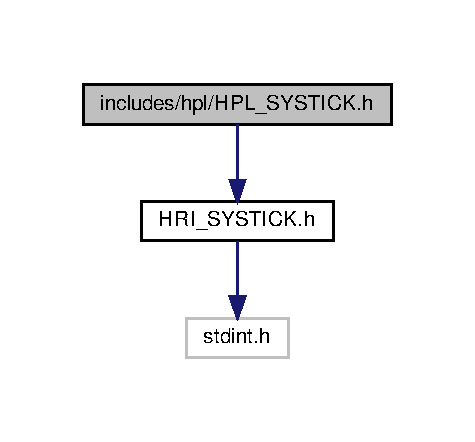
\includegraphics[width=228pt]{HPL__SYSTICK_8h__incl}
\end{center}
\end{figure}
Gráfico de los archivos que directa o indirectamente incluyen a este archivo\+:\nopagebreak
\begin{figure}[H]
\begin{center}
\leavevmode
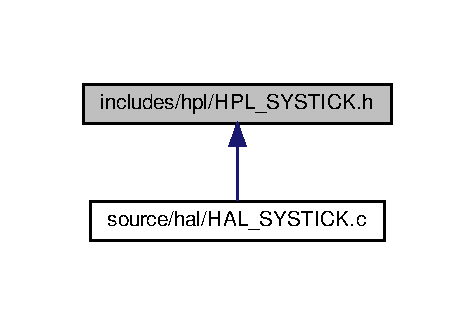
\includegraphics[width=228pt]{HPL__SYSTICK_8h__dep__incl}
\end{center}
\end{figure}
\subsection*{Enumeraciones}
\begin{DoxyCompactItemize}
\item 
\mbox{\Hypertarget{HPL__SYSTICK_8h_a9309dfa382ec580b48d1a8e97a69e673}\label{HPL__SYSTICK_8h_a9309dfa382ec580b48d1a8e97a69e673}} 
enum {\bfseries S\+Y\+S\+T\+I\+C\+K\+\_\+clock\+\_\+source\+\_\+en} \{ {\bfseries S\+Y\+S\+T\+I\+C\+K\+\_\+\+C\+L\+O\+C\+K\+\_\+\+S\+O\+U\+R\+C\+E\+\_\+\+M\+A\+I\+N\+\_\+\+C\+L\+O\+C\+K\+\_\+2} = 0, 
{\bfseries S\+Y\+S\+T\+I\+C\+K\+\_\+\+C\+L\+O\+C\+K\+\_\+\+S\+O\+U\+R\+C\+E\+\_\+\+M\+A\+I\+N\+\_\+\+C\+L\+O\+CK}
 \}
\end{DoxyCompactItemize}
\subsection*{Funciones}
\begin{DoxyCompactItemize}
\item 
\mbox{\Hypertarget{HPL__SYSTICK_8h_af69ec926131faf51078889a25e1ba646}\label{HPL__SYSTICK_8h_af69ec926131faf51078889a25e1ba646}} 
static void {\bfseries S\+Y\+S\+T\+I\+C\+K\+\_\+enable\+\_\+count} (void)
\item 
\mbox{\Hypertarget{HPL__SYSTICK_8h_a29be7583e848cb9322e7377f9a480918}\label{HPL__SYSTICK_8h_a29be7583e848cb9322e7377f9a480918}} 
static void {\bfseries S\+Y\+S\+T\+I\+C\+K\+\_\+disable\+\_\+count} (void)
\item 
\mbox{\Hypertarget{HPL__SYSTICK_8h_a9a7ffbd3089ce51db4963d7aa4fd03e1}\label{HPL__SYSTICK_8h_a9a7ffbd3089ce51db4963d7aa4fd03e1}} 
static void {\bfseries S\+Y\+S\+T\+I\+C\+K\+\_\+enable\+\_\+interrupt} (void)
\item 
\mbox{\Hypertarget{HPL__SYSTICK_8h_a3cf92892f8fadea1990fd50f19474b1f}\label{HPL__SYSTICK_8h_a3cf92892f8fadea1990fd50f19474b1f}} 
static void {\bfseries S\+Y\+S\+T\+I\+C\+K\+\_\+disable\+\_\+interrupt} (void)
\item 
static void \hyperlink{HPL__SYSTICK_8h_a1631a3b564c754b74c904a4977abc930}{S\+Y\+S\+T\+I\+C\+K\+\_\+select\+\_\+clock\+\_\+source} (S\+Y\+S\+T\+I\+C\+K\+\_\+clock\+\_\+source\+\_\+en clock\+\_\+source)
\begin{DoxyCompactList}\small\item\em Seleccion de fuente de clock. \end{DoxyCompactList}\item 
static uint8\+\_\+t \hyperlink{HPL__SYSTICK_8h_a501e38ba8b3ed518fd143b26921e8db1}{S\+Y\+S\+T\+I\+C\+K\+\_\+get\+\_\+count\+\_\+flag} (void)
\begin{DoxyCompactList}\small\item\em Obtener flag de conteo terminado. \end{DoxyCompactList}\item 
\mbox{\Hypertarget{HPL__SYSTICK_8h_a9ca56990dce68fce808a855f8daea3a9}\label{HPL__SYSTICK_8h_a9ca56990dce68fce808a855f8daea3a9}} 
static void \hyperlink{HPL__SYSTICK_8h_a9ca56990dce68fce808a855f8daea3a9}{S\+Y\+S\+T\+I\+C\+K\+\_\+set\+\_\+reload} (uint32\+\_\+t reload)
\begin{DoxyCompactList}\small\item\em Fijar el valor de reload. \end{DoxyCompactList}\item 
\mbox{\Hypertarget{HPL__SYSTICK_8h_aab60c286f8439c8a99ad65527afca7f9}\label{HPL__SYSTICK_8h_aab60c286f8439c8a99ad65527afca7f9}} 
static void \hyperlink{HPL__SYSTICK_8h_aab60c286f8439c8a99ad65527afca7f9}{S\+Y\+S\+T\+I\+C\+K\+\_\+set\+\_\+clear\+\_\+current\+\_\+value} (void)
\begin{DoxyCompactList}\small\item\em Limpiar el conteo actual. \end{DoxyCompactList}\end{DoxyCompactItemize}
\subsection*{Variables}
\begin{DoxyCompactItemize}
\item 
\mbox{\Hypertarget{HPL__SYSTICK_8h_ae93512de27b9aab4f1b225d5bdd2c898}\label{HPL__SYSTICK_8h_ae93512de27b9aab4f1b225d5bdd2c898}} 
volatile \hyperlink{HRI__SYSTICK_8h_structSYSTICK__reg__t}{S\+Y\+S\+T\+I\+C\+K\+\_\+reg\+\_\+t} $\ast$const \hyperlink{HPL__SYSTICK_8h_ae93512de27b9aab4f1b225d5bdd2c898}{S\+Y\+S\+T\+I\+CK}
\begin{DoxyCompactList}\small\item\em Periferico S\+Y\+S\+T\+I\+CK. \end{DoxyCompactList}\end{DoxyCompactItemize}


\subsection{Descripción detallada}
Declaraciones a nivel de abstraccion de periferico del S\+Y\+S\+T\+I\+CK (L\+P\+C845) 

\begin{DoxyAuthor}{Autor}
Augusto Santini 
\end{DoxyAuthor}
\begin{DoxyDate}{Fecha}
6/2019 
\end{DoxyDate}
\begin{DoxyVersion}{Versión}
1.\+0 
\end{DoxyVersion}


\subsection{Documentación de las funciones}
\mbox{\Hypertarget{HPL__SYSTICK_8h_a1631a3b564c754b74c904a4977abc930}\label{HPL__SYSTICK_8h_a1631a3b564c754b74c904a4977abc930}} 
\index{H\+P\+L\+\_\+\+S\+Y\+S\+T\+I\+C\+K.\+h@{H\+P\+L\+\_\+\+S\+Y\+S\+T\+I\+C\+K.\+h}!S\+Y\+S\+T\+I\+C\+K\+\_\+select\+\_\+clock\+\_\+source@{S\+Y\+S\+T\+I\+C\+K\+\_\+select\+\_\+clock\+\_\+source}}
\index{S\+Y\+S\+T\+I\+C\+K\+\_\+select\+\_\+clock\+\_\+source@{S\+Y\+S\+T\+I\+C\+K\+\_\+select\+\_\+clock\+\_\+source}!H\+P\+L\+\_\+\+S\+Y\+S\+T\+I\+C\+K.\+h@{H\+P\+L\+\_\+\+S\+Y\+S\+T\+I\+C\+K.\+h}}
\subsubsection{\texorpdfstring{S\+Y\+S\+T\+I\+C\+K\+\_\+select\+\_\+clock\+\_\+source()}{SYSTICK\_select\_clock\_source()}}
{\footnotesize\ttfamily static void S\+Y\+S\+T\+I\+C\+K\+\_\+select\+\_\+clock\+\_\+source (\begin{DoxyParamCaption}\item[{S\+Y\+S\+T\+I\+C\+K\+\_\+clock\+\_\+source\+\_\+en}]{clock\+\_\+source }\end{DoxyParamCaption})\hspace{0.3cm}{\ttfamily [inline]}, {\ttfamily [static]}}



Seleccion de fuente de clock. 


\begin{DoxyParams}[1]{Parámetros}
\mbox{\tt in}  & {\em clock\+\_\+source} & Fuente deseada \\
\hline
\end{DoxyParams}
\mbox{\Hypertarget{HPL__SYSTICK_8h_a501e38ba8b3ed518fd143b26921e8db1}\label{HPL__SYSTICK_8h_a501e38ba8b3ed518fd143b26921e8db1}} 
\index{H\+P\+L\+\_\+\+S\+Y\+S\+T\+I\+C\+K.\+h@{H\+P\+L\+\_\+\+S\+Y\+S\+T\+I\+C\+K.\+h}!S\+Y\+S\+T\+I\+C\+K\+\_\+get\+\_\+count\+\_\+flag@{S\+Y\+S\+T\+I\+C\+K\+\_\+get\+\_\+count\+\_\+flag}}
\index{S\+Y\+S\+T\+I\+C\+K\+\_\+get\+\_\+count\+\_\+flag@{S\+Y\+S\+T\+I\+C\+K\+\_\+get\+\_\+count\+\_\+flag}!H\+P\+L\+\_\+\+S\+Y\+S\+T\+I\+C\+K.\+h@{H\+P\+L\+\_\+\+S\+Y\+S\+T\+I\+C\+K.\+h}}
\subsubsection{\texorpdfstring{S\+Y\+S\+T\+I\+C\+K\+\_\+get\+\_\+count\+\_\+flag()}{SYSTICK\_get\_count\_flag()}}
{\footnotesize\ttfamily static uint8\+\_\+t S\+Y\+S\+T\+I\+C\+K\+\_\+get\+\_\+count\+\_\+flag (\begin{DoxyParamCaption}\item[{void}]{ }\end{DoxyParamCaption})\hspace{0.3cm}{\ttfamily [inline]}, {\ttfamily [static]}}



Obtener flag de conteo terminado. 

\begin{DoxyReturn}{Devuelve}
Si el S\+Y\+S\+T\+I\+CK habia terminado la cuenta antes de leer el registro, devuelve 1 
\end{DoxyReturn}

\hypertarget{HPL__UART_8h}{}\section{Referencia del Archivo includes/hpl/\+H\+P\+L\+\_\+\+U\+A\+RT.h}
\label{HPL__UART_8h}\index{includes/hpl/\+H\+P\+L\+\_\+\+U\+A\+R\+T.\+h@{includes/hpl/\+H\+P\+L\+\_\+\+U\+A\+R\+T.\+h}}


Declaraciones a nivel de abstraccion de periferico del U\+A\+RT (L\+P\+C845)  


{\ttfamily \#include $<$H\+R\+I\+\_\+\+U\+A\+R\+T.\+h$>$}\newline
Dependencia gráfica adjunta para H\+P\+L\+\_\+\+U\+A\+R\+T.\+h\+:\nopagebreak
\begin{figure}[H]
\begin{center}
\leavevmode
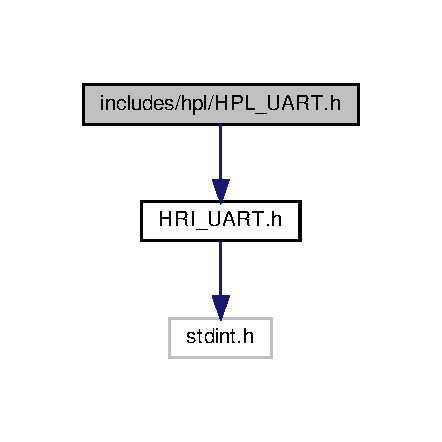
\includegraphics[width=212pt]{d7/d0a/HPL__UART_8h__incl}
\end{center}
\end{figure}
Gráfico de los archivos que directa o indirectamente incluyen a este archivo\+:\nopagebreak
\begin{figure}[H]
\begin{center}
\leavevmode
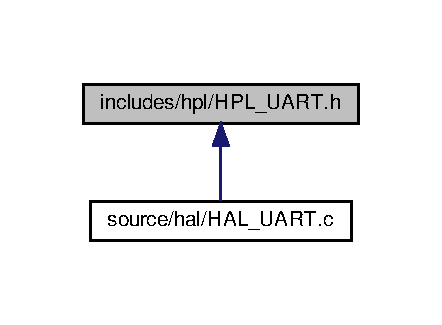
\includegraphics[width=212pt]{d7/df7/HPL__UART_8h__dep__incl}
\end{center}
\end{figure}
\subsection*{Enumeraciones}
\begin{DoxyCompactItemize}
\item 
\mbox{\Hypertarget{HPL__UART_8h_a796c05fb38e1c73458deaff345ed3294}\label{HPL__UART_8h_a796c05fb38e1c73458deaff345ed3294}} 
enum {\bfseries U\+A\+R\+T\+\_\+datalen\+\_\+en} \{ {\bfseries U\+A\+R\+T\+\_\+\+D\+A\+T\+A\+L\+E\+N\+\_\+7\+B\+IT} = 0, 
{\bfseries U\+A\+R\+T\+\_\+\+D\+A\+T\+A\+L\+E\+N\+\_\+8\+B\+IT}, 
{\bfseries U\+A\+R\+T\+\_\+\+D\+A\+T\+A\+L\+E\+N\+\_\+9\+B\+IT}
 \}
\item 
\mbox{\Hypertarget{HPL__UART_8h_af31911af6cc0f77ca0d0bc77f823f080}\label{HPL__UART_8h_af31911af6cc0f77ca0d0bc77f823f080}} 
enum {\bfseries U\+A\+R\+T\+\_\+parity\+\_\+en} \{ {\bfseries U\+A\+R\+T\+\_\+\+P\+A\+R\+I\+T\+Y\+\_\+\+N\+O\+\_\+\+P\+A\+R\+I\+TY} = 0, 
{\bfseries U\+A\+R\+T\+\_\+\+P\+A\+R\+I\+T\+Y\+\_\+\+E\+V\+EN} = 2, 
{\bfseries U\+A\+R\+T\+\_\+\+P\+A\+R\+I\+T\+Y\+\_\+\+O\+DD}
 \}
\item 
\mbox{\Hypertarget{HPL__UART_8h_abf8b1e01f04bb13ce8decef53ae5d669}\label{HPL__UART_8h_abf8b1e01f04bb13ce8decef53ae5d669}} 
enum {\bfseries U\+A\+R\+T\+\_\+stoplen\+\_\+en} \{ {\bfseries U\+A\+R\+T\+\_\+\+S\+T\+O\+P\+L\+E\+N\+\_\+1\+B\+IT} = 0, 
{\bfseries U\+A\+R\+T\+\_\+\+S\+T\+O\+P\+L\+E\+N\+\_\+2\+B\+IT}
 \}
\item 
\mbox{\Hypertarget{HPL__UART_8h_a00ea95868d60656eb21690289c4fe44d}\label{HPL__UART_8h_a00ea95868d60656eb21690289c4fe44d}} 
enum {\bfseries U\+A\+R\+T\+\_\+sync\+\_\+mode\+\_\+en} \{ {\bfseries U\+A\+R\+T\+\_\+\+S\+Y\+N\+C\+\_\+\+M\+O\+D\+E\+\_\+\+A\+S\+Y\+N\+C\+H\+R\+O\+N\+O\+US} = 0, 
{\bfseries U\+A\+R\+T\+\_\+\+S\+Y\+N\+C\+\_\+\+M\+O\+D\+E\+\_\+\+S\+Y\+N\+C\+H\+R\+O\+N\+O\+US}
 \}
\item 
\mbox{\Hypertarget{HPL__UART_8h_ae1947884a2ac95c00385389f6519663a}\label{HPL__UART_8h_ae1947884a2ac95c00385389f6519663a}} 
enum {\bfseries U\+A\+R\+T\+\_\+polarity\+\_\+en} \{ {\bfseries U\+A\+R\+T\+\_\+\+P\+O\+L\+A\+R\+I\+T\+Y\+\_\+\+F\+A\+L\+L\+I\+N\+G\+\_\+\+E\+D\+GE} = 0, 
{\bfseries U\+A\+R\+T\+\_\+\+P\+O\+L\+A\+R\+I\+T\+Y\+\_\+\+R\+I\+S\+I\+N\+G\+\_\+\+E\+D\+GE}
 \}
\item 
\mbox{\Hypertarget{HPL__UART_8h_a67f36818f500257e1ecff7ea64269ac0}\label{HPL__UART_8h_a67f36818f500257e1ecff7ea64269ac0}} 
enum {\bfseries U\+A\+R\+T\+\_\+master\+\_\+mode\+\_\+en} \{ {\bfseries U\+A\+R\+T\+\_\+\+M\+A\+S\+T\+E\+R\+\_\+\+M\+O\+D\+E\+\_\+\+S\+L\+A\+VE} = 0, 
{\bfseries U\+A\+R\+T\+\_\+\+M\+A\+S\+T\+E\+R\+\_\+\+M\+O\+D\+E\+\_\+\+M\+A\+S\+T\+ER}
 \}
\item 
\mbox{\Hypertarget{HPL__UART_8h_a47eb66b5f65368bec4815a519945ce9e}\label{HPL__UART_8h_a47eb66b5f65368bec4815a519945ce9e}} 
enum {\bfseries U\+A\+R\+T\+\_\+output\+\_\+enable\+\_\+pol\+\_\+en} \{ {\bfseries U\+A\+R\+T\+\_\+\+O\+U\+T\+P\+U\+T\+\_\+\+E\+N\+A\+B\+L\+E\+\_\+\+P\+O\+L\+\_\+\+L\+OW} = 0, 
{\bfseries U\+A\+R\+T\+\_\+\+O\+U\+T\+P\+U\+T\+\_\+\+E\+N\+A\+B\+L\+E\+\_\+\+P\+O\+L\+\_\+\+H\+I\+GH}
 \}
\end{DoxyCompactItemize}
\subsection*{Funciones}
\begin{DoxyCompactItemize}
\item 
static void \hyperlink{HPL__UART_8h_a60ea94ef1f8c4a475a418097f6528e38}{U\+A\+R\+T\+\_\+enable} (uint8\+\_\+t inst)
\begin{DoxyCompactList}\small\item\em Habilitacion de una instancia de U\+A\+RT. \end{DoxyCompactList}\item 
static void \hyperlink{HPL__UART_8h_a72c244f57c47439a84c702a30292c93f}{U\+A\+R\+T\+\_\+disable} (uint8\+\_\+t inst)
\begin{DoxyCompactList}\small\item\em Inhabilitacion de una instancia de U\+A\+RT. \end{DoxyCompactList}\item 
static void \hyperlink{HPL__UART_8h_a2d7e997555b8337f4151b8235c254577}{U\+A\+R\+T\+\_\+config\+\_\+data\+\_\+length} (uint8\+\_\+t inst, U\+A\+R\+T\+\_\+datalen\+\_\+en datalen)
\begin{DoxyCompactList}\small\item\em Configurar largo de palabra. \end{DoxyCompactList}\item 
static void \hyperlink{HPL__UART_8h_ac31adf47beb1a678de3be456e1785760}{U\+A\+R\+T\+\_\+config\+\_\+parity} (uint8\+\_\+t inst, U\+A\+R\+T\+\_\+parity\+\_\+en parity)
\begin{DoxyCompactList}\small\item\em Configurar paridad. \end{DoxyCompactList}\item 
static void \hyperlink{HPL__UART_8h_a6fa54c7ccf56777a48cc59183ff565d5}{U\+A\+R\+T\+\_\+config\+\_\+stop\+\_\+bits} (uint8\+\_\+t inst, U\+A\+R\+T\+\_\+stoplen\+\_\+en stop\+\_\+bits)
\begin{DoxyCompactList}\small\item\em Configurar bits de stop. \end{DoxyCompactList}\item 
static void \hyperlink{HPL__UART_8h_adb843edc38133a61cb63a2a1e009bded}{U\+A\+R\+T\+\_\+enable\+\_\+\+C\+TS} (uint8\+\_\+t inst)
\begin{DoxyCompactList}\small\item\em Habilitar C\+TS. \end{DoxyCompactList}\item 
static void \hyperlink{HPL__UART_8h_afa863bf06c40708f540ea49cb7f7b22d}{U\+A\+R\+T\+\_\+disable\+\_\+\+C\+TS} (uint8\+\_\+t inst)
\begin{DoxyCompactList}\small\item\em Inhabilitar C\+TS. \end{DoxyCompactList}\item 
static void \hyperlink{HPL__UART_8h_a1eda22d7fd9ed8dd6998b36df6feeddd}{U\+A\+R\+T\+\_\+config\+\_\+sync\+\_\+mode} (uint8\+\_\+t inst, U\+A\+R\+T\+\_\+sync\+\_\+mode\+\_\+en sync\+\_\+mode)
\begin{DoxyCompactList}\small\item\em Configurar modo asincronico/sincronico. \end{DoxyCompactList}\item 
static void \hyperlink{HPL__UART_8h_a276b09e2c0c47d528632d5d066c16f81}{U\+A\+R\+T\+\_\+config\+\_\+clock\+\_\+polarity} (uint8\+\_\+t inst, U\+A\+R\+T\+\_\+polarity\+\_\+en polarity)
\begin{DoxyCompactList}\small\item\em Configurar polaridad de clock y sampleo (modo sincronico) \end{DoxyCompactList}\item 
static void \hyperlink{HPL__UART_8h_ab7298ad9cba89f80ace8f1efaf8638c0}{U\+A\+R\+T\+\_\+config\+\_\+master\+\_\+mode} (uint8\+\_\+t inst, U\+A\+R\+T\+\_\+master\+\_\+mode\+\_\+en master\+\_\+mode)
\begin{DoxyCompactList}\small\item\em Configurar modo master o slave (modo sincronico) \end{DoxyCompactList}\item 
static void \hyperlink{HPL__UART_8h_a074d4aed5edf289e806f1d88218a6c97}{U\+A\+R\+T\+\_\+enable\+\_\+loopback} (uint8\+\_\+t inst)
\begin{DoxyCompactList}\small\item\em Habilitar modo loopback. \end{DoxyCompactList}\item 
static void \hyperlink{HPL__UART_8h_a55b6baffa18acf57f050f5122b4d3ec2}{U\+A\+R\+T\+\_\+disable\+\_\+loopback} (uint8\+\_\+t inst)
\begin{DoxyCompactList}\small\item\em Inhabilitar modo loopback. \end{DoxyCompactList}\item 
static void \hyperlink{HPL__UART_8h_a548d1856efd63c3e493069a9e4701d47}{U\+A\+R\+T\+\_\+enable\+\_\+\+O\+E\+TA} (uint8\+\_\+t inst)
\begin{DoxyCompactList}\small\item\em Habilitar turnarround para R\+S-\/485. \end{DoxyCompactList}\item 
static void \hyperlink{HPL__UART_8h_a637f0fb6faec69ccc182d942b05c30ad}{U\+A\+R\+T\+\_\+disable\+\_\+\+O\+E\+TA} (uint8\+\_\+t inst)
\begin{DoxyCompactList}\small\item\em Inhabilitar turnarround para R\+S-\/485. \end{DoxyCompactList}\item 
static void \hyperlink{HPL__UART_8h_ae3dee14d1e520e43be355033de4cd0be}{U\+A\+R\+T\+\_\+enable\+\_\+auto\+\_\+address} (uint8\+\_\+t inst)
\begin{DoxyCompactList}\small\item\em Habilitar auto address. \end{DoxyCompactList}\item 
static void \hyperlink{HPL__UART_8h_acb34ed3229bac5bf72f6452c04aa9301}{U\+A\+R\+T\+\_\+disable\+\_\+auto\+\_\+address} (uint8\+\_\+t inst)
\begin{DoxyCompactList}\small\item\em Inhabilitar auto address. \end{DoxyCompactList}\item 
static void \hyperlink{HPL__UART_8h_afb72dd7691b2a459b0d7b04a56c00959}{U\+A\+R\+T\+\_\+enable\+\_\+\+O\+E\+S\+EL} (uint8\+\_\+t inst)
\begin{DoxyCompactList}\small\item\em Habilitar output enable para R\+S-\/485. \end{DoxyCompactList}\item 
static void \hyperlink{HPL__UART_8h_a6e7e8fc43b14a824aa74330e3f7d5644}{U\+A\+R\+T\+\_\+disable\+\_\+\+O\+E\+S\+EL} (uint8\+\_\+t inst)
\begin{DoxyCompactList}\small\item\em Inhabilitar output enable para R\+S-\/485. \end{DoxyCompactList}\item 
static void \hyperlink{HPL__UART_8h_a65e6f135a4b97e50b0cb1976e2cd7b99}{U\+A\+R\+T\+\_\+config\+\_\+\+O\+E\+P\+OL} (uint8\+\_\+t inst, U\+A\+R\+T\+\_\+output\+\_\+enable\+\_\+pol\+\_\+en polarity)
\begin{DoxyCompactList}\small\item\em Configurar polaridad de output enable para R\+S-\/485. \end{DoxyCompactList}\item 
static void \hyperlink{HPL__UART_8h_ac564909bc62813cb8c5ce7047e47233c}{U\+A\+R\+T\+\_\+enable\+\_\+rx\+\_\+invert} (uint8\+\_\+t inst)
\begin{DoxyCompactList}\small\item\em Habilitar inversion para recepcion. \end{DoxyCompactList}\item 
static void \hyperlink{HPL__UART_8h_ae2d3ae09cd93cb1aa7fa5be2075d81fc}{U\+A\+R\+T\+\_\+disable\+\_\+rx\+\_\+invert} (uint8\+\_\+t inst)
\begin{DoxyCompactList}\small\item\em Inhabilitar inversion para recepcion. \end{DoxyCompactList}\item 
static void \hyperlink{HPL__UART_8h_a9dd6130897c185d6813b39770dab0cfc}{U\+A\+R\+T\+\_\+enable\+\_\+tx\+\_\+invert} (uint8\+\_\+t inst)
\begin{DoxyCompactList}\small\item\em Habilitar inversion para transmision. \end{DoxyCompactList}\item 
static void \hyperlink{HPL__UART_8h_adbf8a9a5a097982005d6a221c59bc03c}{U\+A\+R\+T\+\_\+disable\+\_\+tx\+\_\+invert} (uint8\+\_\+t inst)
\begin{DoxyCompactList}\small\item\em Inhabilitar inversion para transmision. \end{DoxyCompactList}\item 
static void \hyperlink{HPL__UART_8h_ad5a36015d19bd584ae2c2587982678f1}{U\+A\+R\+T\+\_\+assert\+\_\+break} (uint8\+\_\+t inst)
\begin{DoxyCompactList}\small\item\em Fijar condicion de break. \end{DoxyCompactList}\item 
static void \hyperlink{HPL__UART_8h_ae3f57ed487940cb7f2c74b4a34ab211d}{U\+A\+R\+T\+\_\+clear\+\_\+break} (uint8\+\_\+t inst)
\begin{DoxyCompactList}\small\item\em Liberar condicion de break. \end{DoxyCompactList}\item 
static void \hyperlink{HPL__UART_8h_ac7a6e6eb689fae8623e6109680aca536}{U\+A\+R\+T\+\_\+enable\+\_\+address\+\_\+detect} (uint8\+\_\+t inst)
\begin{DoxyCompactList}\small\item\em Habilitar address detect. \end{DoxyCompactList}\item 
static void \hyperlink{HPL__UART_8h_aad773171f754d67d8d9350c6b4e694f1}{U\+A\+R\+T\+\_\+disable\+\_\+address\+\_\+detect} (uint8\+\_\+t inst)
\begin{DoxyCompactList}\small\item\em Inhabilitar address detect. \end{DoxyCompactList}\item 
static void \hyperlink{HPL__UART_8h_ae15f63c660e1407beb29a5e64eedec3d}{U\+A\+R\+T\+\_\+enable\+\_\+tx} (uint8\+\_\+t inst)
\begin{DoxyCompactList}\small\item\em Habilitar TX. \end{DoxyCompactList}\item 
static void \hyperlink{HPL__UART_8h_a94332836c25e47f1f6c66a071ea89eb3}{U\+A\+R\+T\+\_\+disable\+\_\+tx} (uint8\+\_\+t inst)
\begin{DoxyCompactList}\small\item\em Inhabilitar TX. \end{DoxyCompactList}\item 
static void \hyperlink{HPL__UART_8h_a9f7bf416557ea8535f1b86be4c9a90ab}{U\+A\+R\+T\+\_\+enable\+\_\+continuous\+\_\+clock} (uint8\+\_\+t inst)
\begin{DoxyCompactList}\small\item\em Habilitar clock continuo (modo sincronico) \end{DoxyCompactList}\item 
static void \hyperlink{HPL__UART_8h_a87535fbfe7b615fdd11abf97eaee25b0}{U\+A\+R\+T\+\_\+disable\+\_\+continuous\+\_\+clock} (uint8\+\_\+t inst)
\begin{DoxyCompactList}\small\item\em Inhabilitar clock continuo (modo sincronico) \end{DoxyCompactList}\item 
static void \hyperlink{HPL__UART_8h_ad224663ac383705b17404c7534f4eb21}{U\+A\+R\+T\+\_\+enable\+\_\+autoclear\+\_\+continuous\+\_\+clock} (uint8\+\_\+t inst)
\begin{DoxyCompactList}\small\item\em Habilitar parada de clock continuo en rx (modo sincronico) \end{DoxyCompactList}\item 
static void \hyperlink{HPL__UART_8h_a21eb263d3bb058110b51a328d32fa7f4}{U\+A\+R\+T\+\_\+disable\+\_\+autoclear\+\_\+continuous\+\_\+clock} (uint8\+\_\+t inst)
\begin{DoxyCompactList}\small\item\em Inhabilitar parada de clock continuo en rx (modo sincronico) \end{DoxyCompactList}\item 
static void \hyperlink{HPL__UART_8h_ab3a476bab8e409c5439561f8cfca18e2}{U\+A\+R\+T\+\_\+enable\+\_\+autobaud} (uint8\+\_\+t inst)
\begin{DoxyCompactList}\small\item\em Habilitar auto baud. \end{DoxyCompactList}\item 
static void \hyperlink{HPL__UART_8h_acea2f97a90e42be62c13acfb7856dbdb}{U\+A\+R\+T\+\_\+disable\+\_\+autobaud} (uint8\+\_\+t inst)
\begin{DoxyCompactList}\small\item\em Inhabilitar auto baud. \end{DoxyCompactList}\item 
static uint8\+\_\+t \hyperlink{HPL__UART_8h_a0a38c27e4a13dcda5b2eb622f1ed4d12}{U\+A\+R\+T\+\_\+get\+\_\+flag\+\_\+\+R\+X\+R\+DY} (uint8\+\_\+t inst)
\begin{DoxyCompactList}\small\item\em Obtener estado del flag R\+X\+R\+DY. \end{DoxyCompactList}\item 
static uint8\+\_\+t \hyperlink{HPL__UART_8h_a4f46deb412f7fae130b02c7acf7d162b}{U\+A\+R\+T\+\_\+get\+\_\+flag\+\_\+\+R\+X\+I\+D\+LE} (uint8\+\_\+t inst)
\begin{DoxyCompactList}\small\item\em Obtener estado del flag R\+X\+I\+D\+LE. \end{DoxyCompactList}\item 
static uint8\+\_\+t \hyperlink{HPL__UART_8h_a5f09c10879826cb24491c3a56b6f1343}{U\+A\+R\+T\+\_\+get\+\_\+flag\+\_\+\+T\+X\+R\+DY} (uint8\+\_\+t inst)
\begin{DoxyCompactList}\small\item\em Obtener estado del flag T\+X\+R\+DY. \end{DoxyCompactList}\item 
static uint8\+\_\+t \hyperlink{HPL__UART_8h_aacdaec4d94056b1cb9b8e3b7e84f23b1}{U\+A\+R\+T\+\_\+get\+\_\+flag\+\_\+\+T\+X\+I\+D\+LE} (uint8\+\_\+t inst)
\begin{DoxyCompactList}\small\item\em Obtener estado del flag T\+X\+I\+D\+LE. \end{DoxyCompactList}\item 
static uint8\+\_\+t \hyperlink{HPL__UART_8h_a6d3ca2cdb52af41a26a3cf850c70a6f0}{U\+A\+R\+T\+\_\+get\+\_\+flag\+\_\+\+C\+TS} (uint8\+\_\+t inst)
\begin{DoxyCompactList}\small\item\em Obtener estado del flag C\+TS. \end{DoxyCompactList}\item 
static uint8\+\_\+t \hyperlink{HPL__UART_8h_ae193da68f5c6b217e32154d0b45e5890}{U\+A\+R\+T\+\_\+get\+\_\+flag\+\_\+\+D\+E\+L\+T\+A\+C\+TS} (uint8\+\_\+t inst)
\begin{DoxyCompactList}\small\item\em Obtener estado del flag D\+E\+L\+T\+A\+C\+TS. \end{DoxyCompactList}\item 
static uint8\+\_\+t \hyperlink{HPL__UART_8h_a9ec2b6662644f148bfbdf9df756d0f6b}{U\+A\+R\+T\+\_\+get\+\_\+flag\+\_\+\+T\+X\+D\+I\+S\+S\+T\+AT} (uint8\+\_\+t inst)
\begin{DoxyCompactList}\small\item\em Obtener estado del flag T\+X\+D\+I\+S\+S\+T\+AT. \end{DoxyCompactList}\item 
static uint8\+\_\+t \hyperlink{HPL__UART_8h_a9ad9e427fae4bdb2fe941dfc124b6e8a}{U\+A\+R\+T\+\_\+get\+\_\+flag\+\_\+\+O\+V\+E\+R\+R\+U\+N\+I\+NT} (uint8\+\_\+t inst)
\begin{DoxyCompactList}\small\item\em Obtener estado del flag O\+V\+E\+R\+R\+U\+N\+I\+NT. \end{DoxyCompactList}\item 
static uint8\+\_\+t \hyperlink{HPL__UART_8h_a697da0aadb5ce6302b62cf42c78e9255}{U\+A\+R\+T\+\_\+get\+\_\+flag\+\_\+\+R\+X\+B\+RK} (uint8\+\_\+t inst)
\begin{DoxyCompactList}\small\item\em Obtener estado del flag R\+X\+B\+RK. \end{DoxyCompactList}\item 
static uint8\+\_\+t \hyperlink{HPL__UART_8h_acd172e5c2d232bea23b54fb83f2914a4}{U\+A\+R\+T\+\_\+get\+\_\+flag\+\_\+\+D\+E\+L\+T\+A\+R\+X\+B\+RK} (uint8\+\_\+t inst)
\begin{DoxyCompactList}\small\item\em Obtener estado del flag D\+E\+L\+T\+A\+R\+X\+B\+RK. \end{DoxyCompactList}\item 
static uint8\+\_\+t \hyperlink{HPL__UART_8h_a35770371558656e90fc7d690a8c80d21}{U\+A\+R\+T\+\_\+get\+\_\+flag\+\_\+\+S\+T\+A\+RT} (uint8\+\_\+t inst)
\begin{DoxyCompactList}\small\item\em Obtener estado del flag S\+T\+A\+RT. \end{DoxyCompactList}\item 
static uint8\+\_\+t \hyperlink{HPL__UART_8h_a87c9594a7c91a613866c5e272a2ac7e8}{U\+A\+R\+T\+\_\+get\+\_\+flag\+\_\+\+F\+R\+A\+M\+E\+R\+R\+I\+NT} (uint8\+\_\+t inst)
\begin{DoxyCompactList}\small\item\em Obtener estado del flag F\+R\+A\+M\+E\+R\+R\+I\+NT. \end{DoxyCompactList}\item 
static uint8\+\_\+t \hyperlink{HPL__UART_8h_acc85a693c44206da0ece7d84f61ac30e}{U\+A\+R\+T\+\_\+get\+\_\+flag\+\_\+\+P\+A\+R\+I\+T\+Y\+E\+R\+R\+I\+NT} (uint8\+\_\+t inst)
\begin{DoxyCompactList}\small\item\em Obtener estado del flag P\+A\+R\+I\+T\+Y\+E\+R\+R\+I\+NT. \end{DoxyCompactList}\item 
static uint8\+\_\+t \hyperlink{HPL__UART_8h_aa6a04ee658410cf5e7b403d0d8b8d0e8}{U\+A\+R\+T\+\_\+get\+\_\+flag\+\_\+\+R\+X\+N\+O\+I\+S\+E\+I\+NT} (uint8\+\_\+t inst)
\begin{DoxyCompactList}\small\item\em Obtener estado del flag R\+X\+N\+O\+I\+S\+E\+I\+NT. \end{DoxyCompactList}\item 
static uint8\+\_\+t \hyperlink{HPL__UART_8h_a3cac097e3d45e71f1382b779dd7380b5}{U\+A\+R\+T\+\_\+get\+\_\+flag\+\_\+\+A\+B\+E\+RR} (uint8\+\_\+t inst)
\begin{DoxyCompactList}\small\item\em Obtener estado del flag A\+B\+E\+RR. \end{DoxyCompactList}\item 
static void \hyperlink{HPL__UART_8h_acaf2fb6f698b7a2aa0bb3089abf5c5b2}{U\+A\+R\+T\+\_\+enable\+\_\+irq\+\_\+\+R\+X\+R\+DY} (uint8\+\_\+t inst)
\begin{DoxyCompactList}\small\item\em Habilitar interrupcion en R\+X\+R\+DY. \end{DoxyCompactList}\item 
static void \hyperlink{HPL__UART_8h_a67e5daacc12049c9f8858ec496d56e7d}{U\+A\+R\+T\+\_\+enable\+\_\+irq\+\_\+\+T\+X\+R\+DY} (uint8\+\_\+t inst)
\begin{DoxyCompactList}\small\item\em Habilitar interrupcion en T\+X\+R\+DY. \end{DoxyCompactList}\item 
static void \hyperlink{HPL__UART_8h_a0a020f19367635f769367e2e03054fa9}{U\+A\+R\+T\+\_\+enable\+\_\+irq\+\_\+\+T\+X\+I\+D\+LE} (uint8\+\_\+t inst)
\begin{DoxyCompactList}\small\item\em Habilitar interrupcion en T\+X\+I\+D\+LE. \end{DoxyCompactList}\item 
static void \hyperlink{HPL__UART_8h_a4eb7d60bfb13475fe2ddc736c5e8eb93}{U\+A\+R\+T\+\_\+enable\+\_\+irq\+\_\+\+D\+E\+L\+T\+A\+C\+TS} (uint8\+\_\+t inst)
\begin{DoxyCompactList}\small\item\em Habilitar interrupcion en D\+E\+L\+T\+A\+C\+TS. \end{DoxyCompactList}\item 
static void \hyperlink{HPL__UART_8h_a3c32cbec74dd3b49e3b283a042bc3c57}{U\+A\+R\+T\+\_\+enable\+\_\+irq\+\_\+\+T\+X\+D\+I\+S\+EN} (uint8\+\_\+t inst)
\begin{DoxyCompactList}\small\item\em Habilitar interrupcion en T\+X\+D\+I\+S\+EN. \end{DoxyCompactList}\item 
static void \hyperlink{HPL__UART_8h_acdfb93dfbd2fdd98b1a03880e3519990}{U\+A\+R\+T\+\_\+enable\+\_\+irq\+\_\+\+O\+V\+E\+R\+R\+UN} (uint8\+\_\+t inst)
\begin{DoxyCompactList}\small\item\em Habilitar interrupcion en O\+V\+E\+R\+R\+UN. \end{DoxyCompactList}\item 
static void \hyperlink{HPL__UART_8h_a228fbb5b2cd0c3b0836c4a9e101affde}{U\+A\+R\+T\+\_\+enable\+\_\+irq\+\_\+\+D\+E\+L\+T\+A\+R\+X\+B\+RK} (uint8\+\_\+t inst)
\begin{DoxyCompactList}\small\item\em Habilitar interrupcion en D\+E\+L\+T\+A\+R\+X\+B\+RK. \end{DoxyCompactList}\item 
static void \hyperlink{HPL__UART_8h_ade5ba836ca877be89d8af0ad5684e499}{U\+A\+R\+T\+\_\+enable\+\_\+irq\+\_\+\+S\+T\+A\+RT} (uint8\+\_\+t inst)
\begin{DoxyCompactList}\small\item\em Habilitar interrupcion en S\+T\+A\+RT. \end{DoxyCompactList}\item 
static void \hyperlink{HPL__UART_8h_a2d53f0e1923c10f35458ea8c32cfaa4e}{U\+A\+R\+T\+\_\+enable\+\_\+irq\+\_\+\+F\+R\+A\+M\+E\+RR} (uint8\+\_\+t inst)
\begin{DoxyCompactList}\small\item\em Habilitar interrupcion en F\+R\+A\+M\+E\+RR. \end{DoxyCompactList}\item 
static void \hyperlink{HPL__UART_8h_a5603d503ae0ef7fa27b016e294401465}{U\+A\+R\+T\+\_\+enable\+\_\+irq\+\_\+\+P\+A\+R\+I\+T\+Y\+E\+RR} (uint8\+\_\+t inst)
\begin{DoxyCompactList}\small\item\em Habilitar interrupcion en P\+A\+R\+I\+T\+Y\+E\+RR. \end{DoxyCompactList}\item 
static void \hyperlink{HPL__UART_8h_a2377f7e2df1e973d9441acf50b015a31}{U\+A\+R\+T\+\_\+enable\+\_\+irq\+\_\+\+R\+X\+N\+O\+I\+SE} (uint8\+\_\+t inst)
\begin{DoxyCompactList}\small\item\em Habilitar interrupcion en R\+X\+N\+O\+I\+SE. \end{DoxyCompactList}\item 
static void \hyperlink{HPL__UART_8h_a99d0d03a351b4f05ee0e93b850f6b974}{U\+A\+R\+T\+\_\+enable\+\_\+irq\+\_\+\+A\+B\+E\+RR} (uint8\+\_\+t inst)
\begin{DoxyCompactList}\small\item\em Habilitar interrupcion en A\+B\+E\+RR. \end{DoxyCompactList}\item 
static void \hyperlink{HPL__UART_8h_a2b358777e3b434033a3fe447b160c411}{U\+A\+R\+T\+\_\+disable\+\_\+irq\+\_\+\+R\+X\+R\+DY} (uint8\+\_\+t inst)
\begin{DoxyCompactList}\small\item\em Inhabilitar interrupcion en R\+X\+R\+DY. \end{DoxyCompactList}\item 
static void \hyperlink{HPL__UART_8h_af136cef6f38e8af29d7d349b2ec72e71}{U\+A\+R\+T\+\_\+disable\+\_\+irq\+\_\+\+T\+X\+R\+DY} (uint8\+\_\+t inst)
\begin{DoxyCompactList}\small\item\em Inhabilitar interrupcion en T\+X\+R\+DY. \end{DoxyCompactList}\item 
static void \hyperlink{HPL__UART_8h_a17ba4a9aaff58a861ad375bceae71e03}{U\+A\+R\+T\+\_\+disable\+\_\+irq\+\_\+\+T\+X\+I\+D\+LE} (uint8\+\_\+t inst)
\begin{DoxyCompactList}\small\item\em Inhabilitar interrupcion en T\+X\+I\+D\+LE. \end{DoxyCompactList}\item 
static void \hyperlink{HPL__UART_8h_ae2eb40bf7d569775009910027d2491fa}{U\+A\+R\+T\+\_\+disable\+\_\+irq\+\_\+\+D\+E\+L\+T\+A\+C\+TS} (uint8\+\_\+t inst)
\begin{DoxyCompactList}\small\item\em Inhabilitar interrupcion en D\+E\+L\+T\+A\+C\+TS. \end{DoxyCompactList}\item 
static void \hyperlink{HPL__UART_8h_ac05f4d358072b91ff81a1f67513249a9}{U\+A\+R\+T\+\_\+disable\+\_\+irq\+\_\+\+T\+X\+D\+I\+S\+EN} (uint8\+\_\+t inst)
\begin{DoxyCompactList}\small\item\em Inhabilitar interrupcion en T\+X\+D\+I\+S\+EN. \end{DoxyCompactList}\item 
static void \hyperlink{HPL__UART_8h_a6314da1442f723439c826725416f27a4}{U\+A\+R\+T\+\_\+disable\+\_\+irq\+\_\+\+O\+V\+E\+R\+R\+UN} (uint8\+\_\+t inst)
\begin{DoxyCompactList}\small\item\em Inhabilitar interrupcion en O\+V\+E\+R\+R\+UN. \end{DoxyCompactList}\item 
static void \hyperlink{HPL__UART_8h_aa4e50763aa7189b3b0473d36133c7db6}{U\+A\+R\+T\+\_\+disable\+\_\+irq\+\_\+\+D\+E\+L\+T\+A\+R\+X\+B\+RK} (uint8\+\_\+t inst)
\begin{DoxyCompactList}\small\item\em Inhabilitar interrupcion en D\+E\+L\+T\+A\+R\+X\+B\+RK. \end{DoxyCompactList}\item 
static void \hyperlink{HPL__UART_8h_a01cc1afc55838004598dd2ef0fbc0d5c}{U\+A\+R\+T\+\_\+disable\+\_\+irq\+\_\+\+S\+T\+A\+RT} (uint8\+\_\+t inst)
\begin{DoxyCompactList}\small\item\em Inhabilitar interrupcion en S\+T\+A\+RT. \end{DoxyCompactList}\item 
static void \hyperlink{HPL__UART_8h_a676103e9aed934b996a593a007e2a543}{U\+A\+R\+T\+\_\+disable\+\_\+irq\+\_\+\+F\+R\+A\+M\+E\+RR} (uint8\+\_\+t inst)
\begin{DoxyCompactList}\small\item\em Inhabilitar interrupcion en F\+R\+A\+M\+E\+RR. \end{DoxyCompactList}\item 
static void \hyperlink{HPL__UART_8h_abcb8a735673c194220f6b66c756b9846}{U\+A\+R\+T\+\_\+disable\+\_\+irq\+\_\+\+P\+A\+R\+I\+T\+Y\+E\+RR} (uint8\+\_\+t inst)
\begin{DoxyCompactList}\small\item\em Inhabilitar interrupcion en P\+A\+R\+I\+T\+Y\+E\+RR. \end{DoxyCompactList}\item 
static void \hyperlink{HPL__UART_8h_a4cb0d65fe92e6a6b9055033cdfc9b648}{U\+A\+R\+T\+\_\+disable\+\_\+irq\+\_\+\+R\+X\+N\+O\+I\+SE} (uint8\+\_\+t inst)
\begin{DoxyCompactList}\small\item\em Inhabilitar interrupcion en R\+X\+N\+O\+I\+SE. \end{DoxyCompactList}\item 
static void \hyperlink{HPL__UART_8h_abe6ff5d5d7a4ad1206248149127289db}{U\+A\+R\+T\+\_\+disable\+\_\+irq\+\_\+\+A\+B\+E\+RR} (uint8\+\_\+t inst)
\begin{DoxyCompactList}\small\item\em Inhabilitar interrupcion en A\+B\+E\+RR. \end{DoxyCompactList}\item 
static uint32\+\_\+t \hyperlink{HPL__UART_8h_aca610990416a62cbc224695315a5b111}{U\+A\+R\+T\+\_\+get\+\_\+data} (uint8\+\_\+t inst)
\begin{DoxyCompactList}\small\item\em Obtener ultimo dato recibido. \end{DoxyCompactList}\item 
static uint32\+\_\+t \hyperlink{HPL__UART_8h_aff70e482771caa020f5185a474fb02ad}{U\+A\+R\+T\+\_\+get\+\_\+data\+\_\+and\+\_\+status} (uint8\+\_\+t inst, uint8\+\_\+t $\ast$frame, uint8\+\_\+t $\ast$parity, uint8\+\_\+t $\ast$noise)
\begin{DoxyCompactList}\small\item\em Obtener ultimo dato recibido con flags de errores. \end{DoxyCompactList}\item 
static void \hyperlink{HPL__UART_8h_a860beffc582ca97a3436cc4e71ed4cf1}{U\+A\+R\+T\+\_\+write\+\_\+data} (uint8\+\_\+t inst, uint32\+\_\+t data)
\begin{DoxyCompactList}\small\item\em Iniciar transmision de dato. \end{DoxyCompactList}\item 
static void \hyperlink{HPL__UART_8h_a2f70265e004dc16b9e60bc1f4404ecb7}{U\+A\+R\+T\+\_\+set\+\_\+\+B\+R\+G\+V\+AL} (uint8\+\_\+t inst, uint32\+\_\+t brg)
\begin{DoxyCompactList}\small\item\em Escribir el registro B\+RG. \end{DoxyCompactList}\item 
static uint8\+\_\+t \hyperlink{HPL__UART_8h_af20adfc399c7f3607c66a2cdc0f0f9cb}{U\+A\+R\+T\+\_\+get\+\_\+irq\+\_\+status\+\_\+\+R\+X\+R\+DY} (uint8\+\_\+t inst)
\begin{DoxyCompactList}\small\item\em Leer estado de interrupcion R\+X\+R\+DY. \end{DoxyCompactList}\item 
static uint8\+\_\+t \hyperlink{HPL__UART_8h_a1133be5dcdeb1081b50b28ec9cb5ec40}{U\+A\+R\+T\+\_\+get\+\_\+irq\+\_\+status\+\_\+\+T\+X\+R\+DY} (uint8\+\_\+t inst)
\begin{DoxyCompactList}\small\item\em Leer estado de interrupcion T\+X\+R\+DY. \end{DoxyCompactList}\item 
static uint8\+\_\+t \hyperlink{HPL__UART_8h_af9f6f58eb87af4b7101607c822b87fc7}{U\+A\+R\+T\+\_\+get\+\_\+irq\+\_\+status\+\_\+\+T\+X\+I\+D\+LE} (uint8\+\_\+t inst)
\begin{DoxyCompactList}\small\item\em Leer estado de interrupcion T\+X\+I\+D\+LE. \end{DoxyCompactList}\item 
static uint8\+\_\+t \hyperlink{HPL__UART_8h_a373007b027ca96327a167a36585a5fdd}{U\+A\+R\+T\+\_\+get\+\_\+irq\+\_\+status\+\_\+\+D\+E\+L\+T\+A\+C\+TS} (uint8\+\_\+t inst)
\begin{DoxyCompactList}\small\item\em Leer estado de interrupcion D\+E\+L\+T\+A\+C\+TS. \end{DoxyCompactList}\item 
static uint8\+\_\+t \hyperlink{HPL__UART_8h_a6bbe318c47b32f5861666ce22cadf799}{U\+A\+R\+T\+\_\+get\+\_\+irq\+\_\+status\+\_\+\+T\+X\+D\+IS} (uint8\+\_\+t inst)
\begin{DoxyCompactList}\small\item\em Leer estado de interrupcion T\+X\+D\+IS. \end{DoxyCompactList}\item 
static uint8\+\_\+t \hyperlink{HPL__UART_8h_a6d1f0e29cc19dfd833463f99a9247cbf}{U\+A\+R\+T\+\_\+get\+\_\+irq\+\_\+status\+\_\+\+O\+V\+E\+R\+R\+UN} (uint8\+\_\+t inst)
\begin{DoxyCompactList}\small\item\em Leer estado de interrupcion O\+V\+E\+R\+R\+UN. \end{DoxyCompactList}\item 
static uint8\+\_\+t \hyperlink{HPL__UART_8h_a3a9c6d5de186621cf5d77d61519e7145}{U\+A\+R\+T\+\_\+get\+\_\+irq\+\_\+status\+\_\+\+D\+E\+L\+T\+A\+R\+X\+B\+RK} (uint8\+\_\+t inst)
\begin{DoxyCompactList}\small\item\em Leer estado de interrupcion D\+E\+L\+T\+A\+R\+X\+B\+RK. \end{DoxyCompactList}\item 
static uint8\+\_\+t \hyperlink{HPL__UART_8h_ac6e104a1262d6b0452403867213e7e31}{U\+A\+R\+T\+\_\+get\+\_\+irq\+\_\+status\+\_\+\+S\+T\+A\+RT} (uint8\+\_\+t inst)
\begin{DoxyCompactList}\small\item\em Leer estado de interrupcion S\+T\+A\+RT. \end{DoxyCompactList}\item 
static uint8\+\_\+t \hyperlink{HPL__UART_8h_afa64fb61c9624838cd22f3383e871e2a}{U\+A\+R\+T\+\_\+get\+\_\+irq\+\_\+status\+\_\+\+F\+R\+A\+M\+E\+RR} (uint8\+\_\+t inst)
\begin{DoxyCompactList}\small\item\em Leer estado de interrupcion F\+R\+A\+M\+E\+RR. \end{DoxyCompactList}\item 
static uint8\+\_\+t \hyperlink{HPL__UART_8h_a32ed88657d025cf96dc84e143fcf077e}{U\+A\+R\+T\+\_\+get\+\_\+irq\+\_\+status\+\_\+\+P\+A\+R\+I\+T\+Y\+E\+RR} (uint8\+\_\+t inst)
\begin{DoxyCompactList}\small\item\em Leer estado de interrupcion P\+A\+R\+I\+T\+Y\+E\+RR. \end{DoxyCompactList}\item 
static uint8\+\_\+t \hyperlink{HPL__UART_8h_af42499a6d4aa15755e974dd90f13824f}{U\+A\+R\+T\+\_\+get\+\_\+irq\+\_\+status\+\_\+\+R\+X\+N\+O\+I\+SE} (uint8\+\_\+t inst)
\begin{DoxyCompactList}\small\item\em Leer estado de interrupcion R\+X\+N\+O\+I\+SE. \end{DoxyCompactList}\item 
static uint8\+\_\+t \hyperlink{HPL__UART_8h_a6eac4ebec02e0b4c1c341ff977c42c12}{U\+A\+R\+T\+\_\+get\+\_\+irq\+\_\+status\+\_\+\+A\+B\+E\+RR} (uint8\+\_\+t inst)
\begin{DoxyCompactList}\small\item\em Leer estado de interrupcion A\+B\+E\+RR. \end{DoxyCompactList}\item 
static void \hyperlink{HPL__UART_8h_aa74ab5994d8b5a31839e04e69f5e1cc5}{U\+A\+R\+T\+\_\+set\+\_\+\+O\+S\+R\+V\+AL} (uint8\+\_\+t inst, uint32\+\_\+t osr)
\begin{DoxyCompactList}\small\item\em Escribir el registro O\+SR. \end{DoxyCompactList}\item 
static void \hyperlink{HPL__UART_8h_ab24db414c0cba6540342e97f22eeb92f}{U\+A\+R\+T\+\_\+set\+\_\+address} (uint8\+\_\+t inst, uint32\+\_\+t addr)
\begin{DoxyCompactList}\small\item\em Escribir el registro A\+D\+DR. \end{DoxyCompactList}\end{DoxyCompactItemize}
\subsection*{Variables}
\begin{DoxyCompactItemize}
\item 
\mbox{\Hypertarget{HPL__UART_8h_addecdf0d8e3b43536541bb22fffb8dbe}\label{HPL__UART_8h_addecdf0d8e3b43536541bb22fffb8dbe}} 
volatile \hyperlink{HRI__UART_8h_d0/d1a/structUART__per__t}{U\+A\+R\+T\+\_\+per\+\_\+t} $\ast$const \hyperlink{HPL__UART_8h_addecdf0d8e3b43536541bb22fffb8dbe}{U\+A\+RT} \mbox{[}$\,$\mbox{]}
\begin{DoxyCompactList}\small\item\em Perifericos U\+S\+A\+RT. \end{DoxyCompactList}\end{DoxyCompactItemize}


\subsection{Descripción detallada}
Declaraciones a nivel de abstraccion de periferico del U\+A\+RT (L\+P\+C845) 

\begin{DoxyAuthor}{Autor}
Augusto Santini 
\end{DoxyAuthor}
\begin{DoxyDate}{Fecha}
6/2019 
\end{DoxyDate}
\begin{DoxyVersion}{Versión}
1.\+0 
\end{DoxyVersion}


\subsection{Documentación de las funciones}
\mbox{\Hypertarget{HPL__UART_8h_a60ea94ef1f8c4a475a418097f6528e38}\label{HPL__UART_8h_a60ea94ef1f8c4a475a418097f6528e38}} 
\index{H\+P\+L\+\_\+\+U\+A\+R\+T.\+h@{H\+P\+L\+\_\+\+U\+A\+R\+T.\+h}!U\+A\+R\+T\+\_\+enable@{U\+A\+R\+T\+\_\+enable}}
\index{U\+A\+R\+T\+\_\+enable@{U\+A\+R\+T\+\_\+enable}!H\+P\+L\+\_\+\+U\+A\+R\+T.\+h@{H\+P\+L\+\_\+\+U\+A\+R\+T.\+h}}
\subsubsection{\texorpdfstring{U\+A\+R\+T\+\_\+enable()}{UART\_enable()}}
{\footnotesize\ttfamily static void U\+A\+R\+T\+\_\+enable (\begin{DoxyParamCaption}\item[{uint8\+\_\+t}]{inst }\end{DoxyParamCaption})\hspace{0.3cm}{\ttfamily [inline]}, {\ttfamily [static]}}



Habilitacion de una instancia de U\+A\+RT. 


\begin{DoxyParams}[1]{Parámetros}
\mbox{\tt in}  & {\em inst} & Instancia a habilitar \\
\hline
\end{DoxyParams}
\mbox{\Hypertarget{HPL__UART_8h_a72c244f57c47439a84c702a30292c93f}\label{HPL__UART_8h_a72c244f57c47439a84c702a30292c93f}} 
\index{H\+P\+L\+\_\+\+U\+A\+R\+T.\+h@{H\+P\+L\+\_\+\+U\+A\+R\+T.\+h}!U\+A\+R\+T\+\_\+disable@{U\+A\+R\+T\+\_\+disable}}
\index{U\+A\+R\+T\+\_\+disable@{U\+A\+R\+T\+\_\+disable}!H\+P\+L\+\_\+\+U\+A\+R\+T.\+h@{H\+P\+L\+\_\+\+U\+A\+R\+T.\+h}}
\subsubsection{\texorpdfstring{U\+A\+R\+T\+\_\+disable()}{UART\_disable()}}
{\footnotesize\ttfamily static void U\+A\+R\+T\+\_\+disable (\begin{DoxyParamCaption}\item[{uint8\+\_\+t}]{inst }\end{DoxyParamCaption})\hspace{0.3cm}{\ttfamily [inline]}, {\ttfamily [static]}}



Inhabilitacion de una instancia de U\+A\+RT. 


\begin{DoxyParams}[1]{Parámetros}
\mbox{\tt in}  & {\em inst} & Instancia a inhabilitar \\
\hline
\end{DoxyParams}
\mbox{\Hypertarget{HPL__UART_8h_a2d7e997555b8337f4151b8235c254577}\label{HPL__UART_8h_a2d7e997555b8337f4151b8235c254577}} 
\index{H\+P\+L\+\_\+\+U\+A\+R\+T.\+h@{H\+P\+L\+\_\+\+U\+A\+R\+T.\+h}!U\+A\+R\+T\+\_\+config\+\_\+data\+\_\+length@{U\+A\+R\+T\+\_\+config\+\_\+data\+\_\+length}}
\index{U\+A\+R\+T\+\_\+config\+\_\+data\+\_\+length@{U\+A\+R\+T\+\_\+config\+\_\+data\+\_\+length}!H\+P\+L\+\_\+\+U\+A\+R\+T.\+h@{H\+P\+L\+\_\+\+U\+A\+R\+T.\+h}}
\subsubsection{\texorpdfstring{U\+A\+R\+T\+\_\+config\+\_\+data\+\_\+length()}{UART\_config\_data\_length()}}
{\footnotesize\ttfamily static void U\+A\+R\+T\+\_\+config\+\_\+data\+\_\+length (\begin{DoxyParamCaption}\item[{uint8\+\_\+t}]{inst,  }\item[{U\+A\+R\+T\+\_\+datalen\+\_\+en}]{datalen }\end{DoxyParamCaption})\hspace{0.3cm}{\ttfamily [inline]}, {\ttfamily [static]}}



Configurar largo de palabra. 


\begin{DoxyParams}[1]{Parámetros}
\mbox{\tt in}  & {\em inst} & Instancia a configurar \\
\hline
\mbox{\tt in}  & {\em datalen} & Seleccion de largo de palabra deseado \\
\hline
\end{DoxyParams}
\mbox{\Hypertarget{HPL__UART_8h_ac31adf47beb1a678de3be456e1785760}\label{HPL__UART_8h_ac31adf47beb1a678de3be456e1785760}} 
\index{H\+P\+L\+\_\+\+U\+A\+R\+T.\+h@{H\+P\+L\+\_\+\+U\+A\+R\+T.\+h}!U\+A\+R\+T\+\_\+config\+\_\+parity@{U\+A\+R\+T\+\_\+config\+\_\+parity}}
\index{U\+A\+R\+T\+\_\+config\+\_\+parity@{U\+A\+R\+T\+\_\+config\+\_\+parity}!H\+P\+L\+\_\+\+U\+A\+R\+T.\+h@{H\+P\+L\+\_\+\+U\+A\+R\+T.\+h}}
\subsubsection{\texorpdfstring{U\+A\+R\+T\+\_\+config\+\_\+parity()}{UART\_config\_parity()}}
{\footnotesize\ttfamily static void U\+A\+R\+T\+\_\+config\+\_\+parity (\begin{DoxyParamCaption}\item[{uint8\+\_\+t}]{inst,  }\item[{U\+A\+R\+T\+\_\+parity\+\_\+en}]{parity }\end{DoxyParamCaption})\hspace{0.3cm}{\ttfamily [inline]}, {\ttfamily [static]}}



Configurar paridad. 


\begin{DoxyParams}[1]{Parámetros}
\mbox{\tt in}  & {\em inst} & Instancia a configurar \\
\hline
\mbox{\tt in}  & {\em parity} & Seleccion de paridad deseada \\
\hline
\end{DoxyParams}
\mbox{\Hypertarget{HPL__UART_8h_a6fa54c7ccf56777a48cc59183ff565d5}\label{HPL__UART_8h_a6fa54c7ccf56777a48cc59183ff565d5}} 
\index{H\+P\+L\+\_\+\+U\+A\+R\+T.\+h@{H\+P\+L\+\_\+\+U\+A\+R\+T.\+h}!U\+A\+R\+T\+\_\+config\+\_\+stop\+\_\+bits@{U\+A\+R\+T\+\_\+config\+\_\+stop\+\_\+bits}}
\index{U\+A\+R\+T\+\_\+config\+\_\+stop\+\_\+bits@{U\+A\+R\+T\+\_\+config\+\_\+stop\+\_\+bits}!H\+P\+L\+\_\+\+U\+A\+R\+T.\+h@{H\+P\+L\+\_\+\+U\+A\+R\+T.\+h}}
\subsubsection{\texorpdfstring{U\+A\+R\+T\+\_\+config\+\_\+stop\+\_\+bits()}{UART\_config\_stop\_bits()}}
{\footnotesize\ttfamily static void U\+A\+R\+T\+\_\+config\+\_\+stop\+\_\+bits (\begin{DoxyParamCaption}\item[{uint8\+\_\+t}]{inst,  }\item[{U\+A\+R\+T\+\_\+stoplen\+\_\+en}]{stop\+\_\+bits }\end{DoxyParamCaption})\hspace{0.3cm}{\ttfamily [inline]}, {\ttfamily [static]}}



Configurar bits de stop. 


\begin{DoxyParams}[1]{Parámetros}
\mbox{\tt in}  & {\em inst} & Instancia a configurar \\
\hline
\mbox{\tt in}  & {\em stop\+\_\+bits} & Seleccion de bits de stop deseados \\
\hline
\end{DoxyParams}
\mbox{\Hypertarget{HPL__UART_8h_adb843edc38133a61cb63a2a1e009bded}\label{HPL__UART_8h_adb843edc38133a61cb63a2a1e009bded}} 
\index{H\+P\+L\+\_\+\+U\+A\+R\+T.\+h@{H\+P\+L\+\_\+\+U\+A\+R\+T.\+h}!U\+A\+R\+T\+\_\+enable\+\_\+\+C\+TS@{U\+A\+R\+T\+\_\+enable\+\_\+\+C\+TS}}
\index{U\+A\+R\+T\+\_\+enable\+\_\+\+C\+TS@{U\+A\+R\+T\+\_\+enable\+\_\+\+C\+TS}!H\+P\+L\+\_\+\+U\+A\+R\+T.\+h@{H\+P\+L\+\_\+\+U\+A\+R\+T.\+h}}
\subsubsection{\texorpdfstring{U\+A\+R\+T\+\_\+enable\+\_\+\+C\+T\+S()}{UART\_enable\_CTS()}}
{\footnotesize\ttfamily static void U\+A\+R\+T\+\_\+enable\+\_\+\+C\+TS (\begin{DoxyParamCaption}\item[{uint8\+\_\+t}]{inst }\end{DoxyParamCaption})\hspace{0.3cm}{\ttfamily [inline]}, {\ttfamily [static]}}



Habilitar C\+TS. 


\begin{DoxyParams}[1]{Parámetros}
\mbox{\tt in}  & {\em inst} & Instancia a habilitar \\
\hline
\end{DoxyParams}
\mbox{\Hypertarget{HPL__UART_8h_afa863bf06c40708f540ea49cb7f7b22d}\label{HPL__UART_8h_afa863bf06c40708f540ea49cb7f7b22d}} 
\index{H\+P\+L\+\_\+\+U\+A\+R\+T.\+h@{H\+P\+L\+\_\+\+U\+A\+R\+T.\+h}!U\+A\+R\+T\+\_\+disable\+\_\+\+C\+TS@{U\+A\+R\+T\+\_\+disable\+\_\+\+C\+TS}}
\index{U\+A\+R\+T\+\_\+disable\+\_\+\+C\+TS@{U\+A\+R\+T\+\_\+disable\+\_\+\+C\+TS}!H\+P\+L\+\_\+\+U\+A\+R\+T.\+h@{H\+P\+L\+\_\+\+U\+A\+R\+T.\+h}}
\subsubsection{\texorpdfstring{U\+A\+R\+T\+\_\+disable\+\_\+\+C\+T\+S()}{UART\_disable\_CTS()}}
{\footnotesize\ttfamily static void U\+A\+R\+T\+\_\+disable\+\_\+\+C\+TS (\begin{DoxyParamCaption}\item[{uint8\+\_\+t}]{inst }\end{DoxyParamCaption})\hspace{0.3cm}{\ttfamily [inline]}, {\ttfamily [static]}}



Inhabilitar C\+TS. 


\begin{DoxyParams}[1]{Parámetros}
\mbox{\tt in}  & {\em inst} & Instancia a inhabilitar \\
\hline
\end{DoxyParams}
\mbox{\Hypertarget{HPL__UART_8h_a1eda22d7fd9ed8dd6998b36df6feeddd}\label{HPL__UART_8h_a1eda22d7fd9ed8dd6998b36df6feeddd}} 
\index{H\+P\+L\+\_\+\+U\+A\+R\+T.\+h@{H\+P\+L\+\_\+\+U\+A\+R\+T.\+h}!U\+A\+R\+T\+\_\+config\+\_\+sync\+\_\+mode@{U\+A\+R\+T\+\_\+config\+\_\+sync\+\_\+mode}}
\index{U\+A\+R\+T\+\_\+config\+\_\+sync\+\_\+mode@{U\+A\+R\+T\+\_\+config\+\_\+sync\+\_\+mode}!H\+P\+L\+\_\+\+U\+A\+R\+T.\+h@{H\+P\+L\+\_\+\+U\+A\+R\+T.\+h}}
\subsubsection{\texorpdfstring{U\+A\+R\+T\+\_\+config\+\_\+sync\+\_\+mode()}{UART\_config\_sync\_mode()}}
{\footnotesize\ttfamily static void U\+A\+R\+T\+\_\+config\+\_\+sync\+\_\+mode (\begin{DoxyParamCaption}\item[{uint8\+\_\+t}]{inst,  }\item[{U\+A\+R\+T\+\_\+sync\+\_\+mode\+\_\+en}]{sync\+\_\+mode }\end{DoxyParamCaption})\hspace{0.3cm}{\ttfamily [inline]}, {\ttfamily [static]}}



Configurar modo asincronico/sincronico. 


\begin{DoxyParams}[1]{Parámetros}
\mbox{\tt in}  & {\em inst} & Instancia a configurar \\
\hline
\mbox{\tt in}  & {\em sync\+\_\+mode} & Modo desesado \\
\hline
\end{DoxyParams}
\mbox{\Hypertarget{HPL__UART_8h_a276b09e2c0c47d528632d5d066c16f81}\label{HPL__UART_8h_a276b09e2c0c47d528632d5d066c16f81}} 
\index{H\+P\+L\+\_\+\+U\+A\+R\+T.\+h@{H\+P\+L\+\_\+\+U\+A\+R\+T.\+h}!U\+A\+R\+T\+\_\+config\+\_\+clock\+\_\+polarity@{U\+A\+R\+T\+\_\+config\+\_\+clock\+\_\+polarity}}
\index{U\+A\+R\+T\+\_\+config\+\_\+clock\+\_\+polarity@{U\+A\+R\+T\+\_\+config\+\_\+clock\+\_\+polarity}!H\+P\+L\+\_\+\+U\+A\+R\+T.\+h@{H\+P\+L\+\_\+\+U\+A\+R\+T.\+h}}
\subsubsection{\texorpdfstring{U\+A\+R\+T\+\_\+config\+\_\+clock\+\_\+polarity()}{UART\_config\_clock\_polarity()}}
{\footnotesize\ttfamily static void U\+A\+R\+T\+\_\+config\+\_\+clock\+\_\+polarity (\begin{DoxyParamCaption}\item[{uint8\+\_\+t}]{inst,  }\item[{U\+A\+R\+T\+\_\+polarity\+\_\+en}]{polarity }\end{DoxyParamCaption})\hspace{0.3cm}{\ttfamily [inline]}, {\ttfamily [static]}}



Configurar polaridad de clock y sampleo (modo sincronico) 


\begin{DoxyParams}[1]{Parámetros}
\mbox{\tt in}  & {\em inst} & Instancia a configurar \\
\hline
\mbox{\tt in}  & {\em polarity} & Polaridad y sampleo desesado \\
\hline
\end{DoxyParams}
\mbox{\Hypertarget{HPL__UART_8h_ab7298ad9cba89f80ace8f1efaf8638c0}\label{HPL__UART_8h_ab7298ad9cba89f80ace8f1efaf8638c0}} 
\index{H\+P\+L\+\_\+\+U\+A\+R\+T.\+h@{H\+P\+L\+\_\+\+U\+A\+R\+T.\+h}!U\+A\+R\+T\+\_\+config\+\_\+master\+\_\+mode@{U\+A\+R\+T\+\_\+config\+\_\+master\+\_\+mode}}
\index{U\+A\+R\+T\+\_\+config\+\_\+master\+\_\+mode@{U\+A\+R\+T\+\_\+config\+\_\+master\+\_\+mode}!H\+P\+L\+\_\+\+U\+A\+R\+T.\+h@{H\+P\+L\+\_\+\+U\+A\+R\+T.\+h}}
\subsubsection{\texorpdfstring{U\+A\+R\+T\+\_\+config\+\_\+master\+\_\+mode()}{UART\_config\_master\_mode()}}
{\footnotesize\ttfamily static void U\+A\+R\+T\+\_\+config\+\_\+master\+\_\+mode (\begin{DoxyParamCaption}\item[{uint8\+\_\+t}]{inst,  }\item[{U\+A\+R\+T\+\_\+master\+\_\+mode\+\_\+en}]{master\+\_\+mode }\end{DoxyParamCaption})\hspace{0.3cm}{\ttfamily [inline]}, {\ttfamily [static]}}



Configurar modo master o slave (modo sincronico) 


\begin{DoxyParams}[1]{Parámetros}
\mbox{\tt in}  & {\em inst} & Instancia a configurar \\
\hline
\mbox{\tt in}  & {\em master\+\_\+mode} & Modo deseado \\
\hline
\end{DoxyParams}
\mbox{\Hypertarget{HPL__UART_8h_a074d4aed5edf289e806f1d88218a6c97}\label{HPL__UART_8h_a074d4aed5edf289e806f1d88218a6c97}} 
\index{H\+P\+L\+\_\+\+U\+A\+R\+T.\+h@{H\+P\+L\+\_\+\+U\+A\+R\+T.\+h}!U\+A\+R\+T\+\_\+enable\+\_\+loopback@{U\+A\+R\+T\+\_\+enable\+\_\+loopback}}
\index{U\+A\+R\+T\+\_\+enable\+\_\+loopback@{U\+A\+R\+T\+\_\+enable\+\_\+loopback}!H\+P\+L\+\_\+\+U\+A\+R\+T.\+h@{H\+P\+L\+\_\+\+U\+A\+R\+T.\+h}}
\subsubsection{\texorpdfstring{U\+A\+R\+T\+\_\+enable\+\_\+loopback()}{UART\_enable\_loopback()}}
{\footnotesize\ttfamily static void U\+A\+R\+T\+\_\+enable\+\_\+loopback (\begin{DoxyParamCaption}\item[{uint8\+\_\+t}]{inst }\end{DoxyParamCaption})\hspace{0.3cm}{\ttfamily [inline]}, {\ttfamily [static]}}



Habilitar modo loopback. 


\begin{DoxyParams}[1]{Parámetros}
\mbox{\tt in}  & {\em inst} & Instancia a configurar \\
\hline
\end{DoxyParams}
\mbox{\Hypertarget{HPL__UART_8h_a55b6baffa18acf57f050f5122b4d3ec2}\label{HPL__UART_8h_a55b6baffa18acf57f050f5122b4d3ec2}} 
\index{H\+P\+L\+\_\+\+U\+A\+R\+T.\+h@{H\+P\+L\+\_\+\+U\+A\+R\+T.\+h}!U\+A\+R\+T\+\_\+disable\+\_\+loopback@{U\+A\+R\+T\+\_\+disable\+\_\+loopback}}
\index{U\+A\+R\+T\+\_\+disable\+\_\+loopback@{U\+A\+R\+T\+\_\+disable\+\_\+loopback}!H\+P\+L\+\_\+\+U\+A\+R\+T.\+h@{H\+P\+L\+\_\+\+U\+A\+R\+T.\+h}}
\subsubsection{\texorpdfstring{U\+A\+R\+T\+\_\+disable\+\_\+loopback()}{UART\_disable\_loopback()}}
{\footnotesize\ttfamily static void U\+A\+R\+T\+\_\+disable\+\_\+loopback (\begin{DoxyParamCaption}\item[{uint8\+\_\+t}]{inst }\end{DoxyParamCaption})\hspace{0.3cm}{\ttfamily [inline]}, {\ttfamily [static]}}



Inhabilitar modo loopback. 


\begin{DoxyParams}[1]{Parámetros}
\mbox{\tt in}  & {\em inst} & Instancia a configurar \\
\hline
\end{DoxyParams}
\mbox{\Hypertarget{HPL__UART_8h_a548d1856efd63c3e493069a9e4701d47}\label{HPL__UART_8h_a548d1856efd63c3e493069a9e4701d47}} 
\index{H\+P\+L\+\_\+\+U\+A\+R\+T.\+h@{H\+P\+L\+\_\+\+U\+A\+R\+T.\+h}!U\+A\+R\+T\+\_\+enable\+\_\+\+O\+E\+TA@{U\+A\+R\+T\+\_\+enable\+\_\+\+O\+E\+TA}}
\index{U\+A\+R\+T\+\_\+enable\+\_\+\+O\+E\+TA@{U\+A\+R\+T\+\_\+enable\+\_\+\+O\+E\+TA}!H\+P\+L\+\_\+\+U\+A\+R\+T.\+h@{H\+P\+L\+\_\+\+U\+A\+R\+T.\+h}}
\subsubsection{\texorpdfstring{U\+A\+R\+T\+\_\+enable\+\_\+\+O\+E\+T\+A()}{UART\_enable\_OETA()}}
{\footnotesize\ttfamily static void U\+A\+R\+T\+\_\+enable\+\_\+\+O\+E\+TA (\begin{DoxyParamCaption}\item[{uint8\+\_\+t}]{inst }\end{DoxyParamCaption})\hspace{0.3cm}{\ttfamily [inline]}, {\ttfamily [static]}}



Habilitar turnarround para R\+S-\/485. 


\begin{DoxyParams}[1]{Parámetros}
\mbox{\tt in}  & {\em inst} & Instancia a configurar \\
\hline
\end{DoxyParams}
\mbox{\Hypertarget{HPL__UART_8h_a637f0fb6faec69ccc182d942b05c30ad}\label{HPL__UART_8h_a637f0fb6faec69ccc182d942b05c30ad}} 
\index{H\+P\+L\+\_\+\+U\+A\+R\+T.\+h@{H\+P\+L\+\_\+\+U\+A\+R\+T.\+h}!U\+A\+R\+T\+\_\+disable\+\_\+\+O\+E\+TA@{U\+A\+R\+T\+\_\+disable\+\_\+\+O\+E\+TA}}
\index{U\+A\+R\+T\+\_\+disable\+\_\+\+O\+E\+TA@{U\+A\+R\+T\+\_\+disable\+\_\+\+O\+E\+TA}!H\+P\+L\+\_\+\+U\+A\+R\+T.\+h@{H\+P\+L\+\_\+\+U\+A\+R\+T.\+h}}
\subsubsection{\texorpdfstring{U\+A\+R\+T\+\_\+disable\+\_\+\+O\+E\+T\+A()}{UART\_disable\_OETA()}}
{\footnotesize\ttfamily static void U\+A\+R\+T\+\_\+disable\+\_\+\+O\+E\+TA (\begin{DoxyParamCaption}\item[{uint8\+\_\+t}]{inst }\end{DoxyParamCaption})\hspace{0.3cm}{\ttfamily [inline]}, {\ttfamily [static]}}



Inhabilitar turnarround para R\+S-\/485. 


\begin{DoxyParams}[1]{Parámetros}
\mbox{\tt in}  & {\em inst} & Instancia a configurar \\
\hline
\end{DoxyParams}
\mbox{\Hypertarget{HPL__UART_8h_ae3dee14d1e520e43be355033de4cd0be}\label{HPL__UART_8h_ae3dee14d1e520e43be355033de4cd0be}} 
\index{H\+P\+L\+\_\+\+U\+A\+R\+T.\+h@{H\+P\+L\+\_\+\+U\+A\+R\+T.\+h}!U\+A\+R\+T\+\_\+enable\+\_\+auto\+\_\+address@{U\+A\+R\+T\+\_\+enable\+\_\+auto\+\_\+address}}
\index{U\+A\+R\+T\+\_\+enable\+\_\+auto\+\_\+address@{U\+A\+R\+T\+\_\+enable\+\_\+auto\+\_\+address}!H\+P\+L\+\_\+\+U\+A\+R\+T.\+h@{H\+P\+L\+\_\+\+U\+A\+R\+T.\+h}}
\subsubsection{\texorpdfstring{U\+A\+R\+T\+\_\+enable\+\_\+auto\+\_\+address()}{UART\_enable\_auto\_address()}}
{\footnotesize\ttfamily static void U\+A\+R\+T\+\_\+enable\+\_\+auto\+\_\+address (\begin{DoxyParamCaption}\item[{uint8\+\_\+t}]{inst }\end{DoxyParamCaption})\hspace{0.3cm}{\ttfamily [inline]}, {\ttfamily [static]}}



Habilitar auto address. 


\begin{DoxyParams}[1]{Parámetros}
\mbox{\tt in}  & {\em inst} & Instancia a configurar \\
\hline
\end{DoxyParams}
\mbox{\Hypertarget{HPL__UART_8h_acb34ed3229bac5bf72f6452c04aa9301}\label{HPL__UART_8h_acb34ed3229bac5bf72f6452c04aa9301}} 
\index{H\+P\+L\+\_\+\+U\+A\+R\+T.\+h@{H\+P\+L\+\_\+\+U\+A\+R\+T.\+h}!U\+A\+R\+T\+\_\+disable\+\_\+auto\+\_\+address@{U\+A\+R\+T\+\_\+disable\+\_\+auto\+\_\+address}}
\index{U\+A\+R\+T\+\_\+disable\+\_\+auto\+\_\+address@{U\+A\+R\+T\+\_\+disable\+\_\+auto\+\_\+address}!H\+P\+L\+\_\+\+U\+A\+R\+T.\+h@{H\+P\+L\+\_\+\+U\+A\+R\+T.\+h}}
\subsubsection{\texorpdfstring{U\+A\+R\+T\+\_\+disable\+\_\+auto\+\_\+address()}{UART\_disable\_auto\_address()}}
{\footnotesize\ttfamily static void U\+A\+R\+T\+\_\+disable\+\_\+auto\+\_\+address (\begin{DoxyParamCaption}\item[{uint8\+\_\+t}]{inst }\end{DoxyParamCaption})\hspace{0.3cm}{\ttfamily [inline]}, {\ttfamily [static]}}



Inhabilitar auto address. 


\begin{DoxyParams}[1]{Parámetros}
\mbox{\tt in}  & {\em inst} & Instancia a configurar \\
\hline
\end{DoxyParams}
\mbox{\Hypertarget{HPL__UART_8h_afb72dd7691b2a459b0d7b04a56c00959}\label{HPL__UART_8h_afb72dd7691b2a459b0d7b04a56c00959}} 
\index{H\+P\+L\+\_\+\+U\+A\+R\+T.\+h@{H\+P\+L\+\_\+\+U\+A\+R\+T.\+h}!U\+A\+R\+T\+\_\+enable\+\_\+\+O\+E\+S\+EL@{U\+A\+R\+T\+\_\+enable\+\_\+\+O\+E\+S\+EL}}
\index{U\+A\+R\+T\+\_\+enable\+\_\+\+O\+E\+S\+EL@{U\+A\+R\+T\+\_\+enable\+\_\+\+O\+E\+S\+EL}!H\+P\+L\+\_\+\+U\+A\+R\+T.\+h@{H\+P\+L\+\_\+\+U\+A\+R\+T.\+h}}
\subsubsection{\texorpdfstring{U\+A\+R\+T\+\_\+enable\+\_\+\+O\+E\+S\+E\+L()}{UART\_enable\_OESEL()}}
{\footnotesize\ttfamily static void U\+A\+R\+T\+\_\+enable\+\_\+\+O\+E\+S\+EL (\begin{DoxyParamCaption}\item[{uint8\+\_\+t}]{inst }\end{DoxyParamCaption})\hspace{0.3cm}{\ttfamily [inline]}, {\ttfamily [static]}}



Habilitar output enable para R\+S-\/485. 


\begin{DoxyParams}[1]{Parámetros}
\mbox{\tt in}  & {\em inst} & Instancia a configurar \\
\hline
\end{DoxyParams}
\mbox{\Hypertarget{HPL__UART_8h_a6e7e8fc43b14a824aa74330e3f7d5644}\label{HPL__UART_8h_a6e7e8fc43b14a824aa74330e3f7d5644}} 
\index{H\+P\+L\+\_\+\+U\+A\+R\+T.\+h@{H\+P\+L\+\_\+\+U\+A\+R\+T.\+h}!U\+A\+R\+T\+\_\+disable\+\_\+\+O\+E\+S\+EL@{U\+A\+R\+T\+\_\+disable\+\_\+\+O\+E\+S\+EL}}
\index{U\+A\+R\+T\+\_\+disable\+\_\+\+O\+E\+S\+EL@{U\+A\+R\+T\+\_\+disable\+\_\+\+O\+E\+S\+EL}!H\+P\+L\+\_\+\+U\+A\+R\+T.\+h@{H\+P\+L\+\_\+\+U\+A\+R\+T.\+h}}
\subsubsection{\texorpdfstring{U\+A\+R\+T\+\_\+disable\+\_\+\+O\+E\+S\+E\+L()}{UART\_disable\_OESEL()}}
{\footnotesize\ttfamily static void U\+A\+R\+T\+\_\+disable\+\_\+\+O\+E\+S\+EL (\begin{DoxyParamCaption}\item[{uint8\+\_\+t}]{inst }\end{DoxyParamCaption})\hspace{0.3cm}{\ttfamily [inline]}, {\ttfamily [static]}}



Inhabilitar output enable para R\+S-\/485. 


\begin{DoxyParams}[1]{Parámetros}
\mbox{\tt in}  & {\em inst} & Instancia a configurar \\
\hline
\end{DoxyParams}
\mbox{\Hypertarget{HPL__UART_8h_a65e6f135a4b97e50b0cb1976e2cd7b99}\label{HPL__UART_8h_a65e6f135a4b97e50b0cb1976e2cd7b99}} 
\index{H\+P\+L\+\_\+\+U\+A\+R\+T.\+h@{H\+P\+L\+\_\+\+U\+A\+R\+T.\+h}!U\+A\+R\+T\+\_\+config\+\_\+\+O\+E\+P\+OL@{U\+A\+R\+T\+\_\+config\+\_\+\+O\+E\+P\+OL}}
\index{U\+A\+R\+T\+\_\+config\+\_\+\+O\+E\+P\+OL@{U\+A\+R\+T\+\_\+config\+\_\+\+O\+E\+P\+OL}!H\+P\+L\+\_\+\+U\+A\+R\+T.\+h@{H\+P\+L\+\_\+\+U\+A\+R\+T.\+h}}
\subsubsection{\texorpdfstring{U\+A\+R\+T\+\_\+config\+\_\+\+O\+E\+P\+O\+L()}{UART\_config\_OEPOL()}}
{\footnotesize\ttfamily static void U\+A\+R\+T\+\_\+config\+\_\+\+O\+E\+P\+OL (\begin{DoxyParamCaption}\item[{uint8\+\_\+t}]{inst,  }\item[{U\+A\+R\+T\+\_\+output\+\_\+enable\+\_\+pol\+\_\+en}]{polarity }\end{DoxyParamCaption})\hspace{0.3cm}{\ttfamily [inline]}, {\ttfamily [static]}}



Configurar polaridad de output enable para R\+S-\/485. 


\begin{DoxyParams}[1]{Parámetros}
\mbox{\tt in}  & {\em inst} & Instancia a configurar \\
\hline
\end{DoxyParams}
\mbox{\Hypertarget{HPL__UART_8h_ac564909bc62813cb8c5ce7047e47233c}\label{HPL__UART_8h_ac564909bc62813cb8c5ce7047e47233c}} 
\index{H\+P\+L\+\_\+\+U\+A\+R\+T.\+h@{H\+P\+L\+\_\+\+U\+A\+R\+T.\+h}!U\+A\+R\+T\+\_\+enable\+\_\+rx\+\_\+invert@{U\+A\+R\+T\+\_\+enable\+\_\+rx\+\_\+invert}}
\index{U\+A\+R\+T\+\_\+enable\+\_\+rx\+\_\+invert@{U\+A\+R\+T\+\_\+enable\+\_\+rx\+\_\+invert}!H\+P\+L\+\_\+\+U\+A\+R\+T.\+h@{H\+P\+L\+\_\+\+U\+A\+R\+T.\+h}}
\subsubsection{\texorpdfstring{U\+A\+R\+T\+\_\+enable\+\_\+rx\+\_\+invert()}{UART\_enable\_rx\_invert()}}
{\footnotesize\ttfamily static void U\+A\+R\+T\+\_\+enable\+\_\+rx\+\_\+invert (\begin{DoxyParamCaption}\item[{uint8\+\_\+t}]{inst }\end{DoxyParamCaption})\hspace{0.3cm}{\ttfamily [inline]}, {\ttfamily [static]}}



Habilitar inversion para recepcion. 


\begin{DoxyParams}[1]{Parámetros}
\mbox{\tt in}  & {\em inst} & Instancia a configurar \\
\hline
\end{DoxyParams}
\mbox{\Hypertarget{HPL__UART_8h_ae2d3ae09cd93cb1aa7fa5be2075d81fc}\label{HPL__UART_8h_ae2d3ae09cd93cb1aa7fa5be2075d81fc}} 
\index{H\+P\+L\+\_\+\+U\+A\+R\+T.\+h@{H\+P\+L\+\_\+\+U\+A\+R\+T.\+h}!U\+A\+R\+T\+\_\+disable\+\_\+rx\+\_\+invert@{U\+A\+R\+T\+\_\+disable\+\_\+rx\+\_\+invert}}
\index{U\+A\+R\+T\+\_\+disable\+\_\+rx\+\_\+invert@{U\+A\+R\+T\+\_\+disable\+\_\+rx\+\_\+invert}!H\+P\+L\+\_\+\+U\+A\+R\+T.\+h@{H\+P\+L\+\_\+\+U\+A\+R\+T.\+h}}
\subsubsection{\texorpdfstring{U\+A\+R\+T\+\_\+disable\+\_\+rx\+\_\+invert()}{UART\_disable\_rx\_invert()}}
{\footnotesize\ttfamily static void U\+A\+R\+T\+\_\+disable\+\_\+rx\+\_\+invert (\begin{DoxyParamCaption}\item[{uint8\+\_\+t}]{inst }\end{DoxyParamCaption})\hspace{0.3cm}{\ttfamily [inline]}, {\ttfamily [static]}}



Inhabilitar inversion para recepcion. 


\begin{DoxyParams}[1]{Parámetros}
\mbox{\tt in}  & {\em inst} & Instancia a configurar \\
\hline
\end{DoxyParams}
\mbox{\Hypertarget{HPL__UART_8h_a9dd6130897c185d6813b39770dab0cfc}\label{HPL__UART_8h_a9dd6130897c185d6813b39770dab0cfc}} 
\index{H\+P\+L\+\_\+\+U\+A\+R\+T.\+h@{H\+P\+L\+\_\+\+U\+A\+R\+T.\+h}!U\+A\+R\+T\+\_\+enable\+\_\+tx\+\_\+invert@{U\+A\+R\+T\+\_\+enable\+\_\+tx\+\_\+invert}}
\index{U\+A\+R\+T\+\_\+enable\+\_\+tx\+\_\+invert@{U\+A\+R\+T\+\_\+enable\+\_\+tx\+\_\+invert}!H\+P\+L\+\_\+\+U\+A\+R\+T.\+h@{H\+P\+L\+\_\+\+U\+A\+R\+T.\+h}}
\subsubsection{\texorpdfstring{U\+A\+R\+T\+\_\+enable\+\_\+tx\+\_\+invert()}{UART\_enable\_tx\_invert()}}
{\footnotesize\ttfamily static void U\+A\+R\+T\+\_\+enable\+\_\+tx\+\_\+invert (\begin{DoxyParamCaption}\item[{uint8\+\_\+t}]{inst }\end{DoxyParamCaption})\hspace{0.3cm}{\ttfamily [inline]}, {\ttfamily [static]}}



Habilitar inversion para transmision. 


\begin{DoxyParams}[1]{Parámetros}
\mbox{\tt in}  & {\em inst} & Instancia a configurar \\
\hline
\end{DoxyParams}
\mbox{\Hypertarget{HPL__UART_8h_adbf8a9a5a097982005d6a221c59bc03c}\label{HPL__UART_8h_adbf8a9a5a097982005d6a221c59bc03c}} 
\index{H\+P\+L\+\_\+\+U\+A\+R\+T.\+h@{H\+P\+L\+\_\+\+U\+A\+R\+T.\+h}!U\+A\+R\+T\+\_\+disable\+\_\+tx\+\_\+invert@{U\+A\+R\+T\+\_\+disable\+\_\+tx\+\_\+invert}}
\index{U\+A\+R\+T\+\_\+disable\+\_\+tx\+\_\+invert@{U\+A\+R\+T\+\_\+disable\+\_\+tx\+\_\+invert}!H\+P\+L\+\_\+\+U\+A\+R\+T.\+h@{H\+P\+L\+\_\+\+U\+A\+R\+T.\+h}}
\subsubsection{\texorpdfstring{U\+A\+R\+T\+\_\+disable\+\_\+tx\+\_\+invert()}{UART\_disable\_tx\_invert()}}
{\footnotesize\ttfamily static void U\+A\+R\+T\+\_\+disable\+\_\+tx\+\_\+invert (\begin{DoxyParamCaption}\item[{uint8\+\_\+t}]{inst }\end{DoxyParamCaption})\hspace{0.3cm}{\ttfamily [inline]}, {\ttfamily [static]}}



Inhabilitar inversion para transmision. 


\begin{DoxyParams}[1]{Parámetros}
\mbox{\tt in}  & {\em inst} & Instancia a configurar \\
\hline
\end{DoxyParams}
\mbox{\Hypertarget{HPL__UART_8h_ad5a36015d19bd584ae2c2587982678f1}\label{HPL__UART_8h_ad5a36015d19bd584ae2c2587982678f1}} 
\index{H\+P\+L\+\_\+\+U\+A\+R\+T.\+h@{H\+P\+L\+\_\+\+U\+A\+R\+T.\+h}!U\+A\+R\+T\+\_\+assert\+\_\+break@{U\+A\+R\+T\+\_\+assert\+\_\+break}}
\index{U\+A\+R\+T\+\_\+assert\+\_\+break@{U\+A\+R\+T\+\_\+assert\+\_\+break}!H\+P\+L\+\_\+\+U\+A\+R\+T.\+h@{H\+P\+L\+\_\+\+U\+A\+R\+T.\+h}}
\subsubsection{\texorpdfstring{U\+A\+R\+T\+\_\+assert\+\_\+break()}{UART\_assert\_break()}}
{\footnotesize\ttfamily static void U\+A\+R\+T\+\_\+assert\+\_\+break (\begin{DoxyParamCaption}\item[{uint8\+\_\+t}]{inst }\end{DoxyParamCaption})\hspace{0.3cm}{\ttfamily [inline]}, {\ttfamily [static]}}



Fijar condicion de break. 


\begin{DoxyParams}[1]{Parámetros}
\mbox{\tt in}  & {\em inst} & Instancia a configurar \\
\hline
\end{DoxyParams}
\mbox{\Hypertarget{HPL__UART_8h_ae3f57ed487940cb7f2c74b4a34ab211d}\label{HPL__UART_8h_ae3f57ed487940cb7f2c74b4a34ab211d}} 
\index{H\+P\+L\+\_\+\+U\+A\+R\+T.\+h@{H\+P\+L\+\_\+\+U\+A\+R\+T.\+h}!U\+A\+R\+T\+\_\+clear\+\_\+break@{U\+A\+R\+T\+\_\+clear\+\_\+break}}
\index{U\+A\+R\+T\+\_\+clear\+\_\+break@{U\+A\+R\+T\+\_\+clear\+\_\+break}!H\+P\+L\+\_\+\+U\+A\+R\+T.\+h@{H\+P\+L\+\_\+\+U\+A\+R\+T.\+h}}
\subsubsection{\texorpdfstring{U\+A\+R\+T\+\_\+clear\+\_\+break()}{UART\_clear\_break()}}
{\footnotesize\ttfamily static void U\+A\+R\+T\+\_\+clear\+\_\+break (\begin{DoxyParamCaption}\item[{uint8\+\_\+t}]{inst }\end{DoxyParamCaption})\hspace{0.3cm}{\ttfamily [inline]}, {\ttfamily [static]}}



Liberar condicion de break. 


\begin{DoxyParams}[1]{Parámetros}
\mbox{\tt in}  & {\em inst} & Instancia a configurar \\
\hline
\end{DoxyParams}
\mbox{\Hypertarget{HPL__UART_8h_ac7a6e6eb689fae8623e6109680aca536}\label{HPL__UART_8h_ac7a6e6eb689fae8623e6109680aca536}} 
\index{H\+P\+L\+\_\+\+U\+A\+R\+T.\+h@{H\+P\+L\+\_\+\+U\+A\+R\+T.\+h}!U\+A\+R\+T\+\_\+enable\+\_\+address\+\_\+detect@{U\+A\+R\+T\+\_\+enable\+\_\+address\+\_\+detect}}
\index{U\+A\+R\+T\+\_\+enable\+\_\+address\+\_\+detect@{U\+A\+R\+T\+\_\+enable\+\_\+address\+\_\+detect}!H\+P\+L\+\_\+\+U\+A\+R\+T.\+h@{H\+P\+L\+\_\+\+U\+A\+R\+T.\+h}}
\subsubsection{\texorpdfstring{U\+A\+R\+T\+\_\+enable\+\_\+address\+\_\+detect()}{UART\_enable\_address\_detect()}}
{\footnotesize\ttfamily static void U\+A\+R\+T\+\_\+enable\+\_\+address\+\_\+detect (\begin{DoxyParamCaption}\item[{uint8\+\_\+t}]{inst }\end{DoxyParamCaption})\hspace{0.3cm}{\ttfamily [inline]}, {\ttfamily [static]}}



Habilitar address detect. 


\begin{DoxyParams}[1]{Parámetros}
\mbox{\tt in}  & {\em inst} & Instancia a configurar \\
\hline
\end{DoxyParams}
\mbox{\Hypertarget{HPL__UART_8h_aad773171f754d67d8d9350c6b4e694f1}\label{HPL__UART_8h_aad773171f754d67d8d9350c6b4e694f1}} 
\index{H\+P\+L\+\_\+\+U\+A\+R\+T.\+h@{H\+P\+L\+\_\+\+U\+A\+R\+T.\+h}!U\+A\+R\+T\+\_\+disable\+\_\+address\+\_\+detect@{U\+A\+R\+T\+\_\+disable\+\_\+address\+\_\+detect}}
\index{U\+A\+R\+T\+\_\+disable\+\_\+address\+\_\+detect@{U\+A\+R\+T\+\_\+disable\+\_\+address\+\_\+detect}!H\+P\+L\+\_\+\+U\+A\+R\+T.\+h@{H\+P\+L\+\_\+\+U\+A\+R\+T.\+h}}
\subsubsection{\texorpdfstring{U\+A\+R\+T\+\_\+disable\+\_\+address\+\_\+detect()}{UART\_disable\_address\_detect()}}
{\footnotesize\ttfamily static void U\+A\+R\+T\+\_\+disable\+\_\+address\+\_\+detect (\begin{DoxyParamCaption}\item[{uint8\+\_\+t}]{inst }\end{DoxyParamCaption})\hspace{0.3cm}{\ttfamily [inline]}, {\ttfamily [static]}}



Inhabilitar address detect. 


\begin{DoxyParams}[1]{Parámetros}
\mbox{\tt in}  & {\em inst} & Instancia a configurar \\
\hline
\end{DoxyParams}
\mbox{\Hypertarget{HPL__UART_8h_ae15f63c660e1407beb29a5e64eedec3d}\label{HPL__UART_8h_ae15f63c660e1407beb29a5e64eedec3d}} 
\index{H\+P\+L\+\_\+\+U\+A\+R\+T.\+h@{H\+P\+L\+\_\+\+U\+A\+R\+T.\+h}!U\+A\+R\+T\+\_\+enable\+\_\+tx@{U\+A\+R\+T\+\_\+enable\+\_\+tx}}
\index{U\+A\+R\+T\+\_\+enable\+\_\+tx@{U\+A\+R\+T\+\_\+enable\+\_\+tx}!H\+P\+L\+\_\+\+U\+A\+R\+T.\+h@{H\+P\+L\+\_\+\+U\+A\+R\+T.\+h}}
\subsubsection{\texorpdfstring{U\+A\+R\+T\+\_\+enable\+\_\+tx()}{UART\_enable\_tx()}}
{\footnotesize\ttfamily static void U\+A\+R\+T\+\_\+enable\+\_\+tx (\begin{DoxyParamCaption}\item[{uint8\+\_\+t}]{inst }\end{DoxyParamCaption})\hspace{0.3cm}{\ttfamily [inline]}, {\ttfamily [static]}}



Habilitar TX. 


\begin{DoxyParams}[1]{Parámetros}
\mbox{\tt in}  & {\em inst} & Instancia a configurar \\
\hline
\end{DoxyParams}
\mbox{\Hypertarget{HPL__UART_8h_a94332836c25e47f1f6c66a071ea89eb3}\label{HPL__UART_8h_a94332836c25e47f1f6c66a071ea89eb3}} 
\index{H\+P\+L\+\_\+\+U\+A\+R\+T.\+h@{H\+P\+L\+\_\+\+U\+A\+R\+T.\+h}!U\+A\+R\+T\+\_\+disable\+\_\+tx@{U\+A\+R\+T\+\_\+disable\+\_\+tx}}
\index{U\+A\+R\+T\+\_\+disable\+\_\+tx@{U\+A\+R\+T\+\_\+disable\+\_\+tx}!H\+P\+L\+\_\+\+U\+A\+R\+T.\+h@{H\+P\+L\+\_\+\+U\+A\+R\+T.\+h}}
\subsubsection{\texorpdfstring{U\+A\+R\+T\+\_\+disable\+\_\+tx()}{UART\_disable\_tx()}}
{\footnotesize\ttfamily static void U\+A\+R\+T\+\_\+disable\+\_\+tx (\begin{DoxyParamCaption}\item[{uint8\+\_\+t}]{inst }\end{DoxyParamCaption})\hspace{0.3cm}{\ttfamily [inline]}, {\ttfamily [static]}}



Inhabilitar TX. 


\begin{DoxyParams}[1]{Parámetros}
\mbox{\tt in}  & {\em inst} & Instancia a configurar \\
\hline
\end{DoxyParams}
\mbox{\Hypertarget{HPL__UART_8h_a9f7bf416557ea8535f1b86be4c9a90ab}\label{HPL__UART_8h_a9f7bf416557ea8535f1b86be4c9a90ab}} 
\index{H\+P\+L\+\_\+\+U\+A\+R\+T.\+h@{H\+P\+L\+\_\+\+U\+A\+R\+T.\+h}!U\+A\+R\+T\+\_\+enable\+\_\+continuous\+\_\+clock@{U\+A\+R\+T\+\_\+enable\+\_\+continuous\+\_\+clock}}
\index{U\+A\+R\+T\+\_\+enable\+\_\+continuous\+\_\+clock@{U\+A\+R\+T\+\_\+enable\+\_\+continuous\+\_\+clock}!H\+P\+L\+\_\+\+U\+A\+R\+T.\+h@{H\+P\+L\+\_\+\+U\+A\+R\+T.\+h}}
\subsubsection{\texorpdfstring{U\+A\+R\+T\+\_\+enable\+\_\+continuous\+\_\+clock()}{UART\_enable\_continuous\_clock()}}
{\footnotesize\ttfamily static void U\+A\+R\+T\+\_\+enable\+\_\+continuous\+\_\+clock (\begin{DoxyParamCaption}\item[{uint8\+\_\+t}]{inst }\end{DoxyParamCaption})\hspace{0.3cm}{\ttfamily [inline]}, {\ttfamily [static]}}



Habilitar clock continuo (modo sincronico) 


\begin{DoxyParams}[1]{Parámetros}
\mbox{\tt in}  & {\em inst} & Instancia a configurar \\
\hline
\end{DoxyParams}
\mbox{\Hypertarget{HPL__UART_8h_a87535fbfe7b615fdd11abf97eaee25b0}\label{HPL__UART_8h_a87535fbfe7b615fdd11abf97eaee25b0}} 
\index{H\+P\+L\+\_\+\+U\+A\+R\+T.\+h@{H\+P\+L\+\_\+\+U\+A\+R\+T.\+h}!U\+A\+R\+T\+\_\+disable\+\_\+continuous\+\_\+clock@{U\+A\+R\+T\+\_\+disable\+\_\+continuous\+\_\+clock}}
\index{U\+A\+R\+T\+\_\+disable\+\_\+continuous\+\_\+clock@{U\+A\+R\+T\+\_\+disable\+\_\+continuous\+\_\+clock}!H\+P\+L\+\_\+\+U\+A\+R\+T.\+h@{H\+P\+L\+\_\+\+U\+A\+R\+T.\+h}}
\subsubsection{\texorpdfstring{U\+A\+R\+T\+\_\+disable\+\_\+continuous\+\_\+clock()}{UART\_disable\_continuous\_clock()}}
{\footnotesize\ttfamily static void U\+A\+R\+T\+\_\+disable\+\_\+continuous\+\_\+clock (\begin{DoxyParamCaption}\item[{uint8\+\_\+t}]{inst }\end{DoxyParamCaption})\hspace{0.3cm}{\ttfamily [inline]}, {\ttfamily [static]}}



Inhabilitar clock continuo (modo sincronico) 


\begin{DoxyParams}[1]{Parámetros}
\mbox{\tt in}  & {\em inst} & Instancia a configurar \\
\hline
\end{DoxyParams}
\mbox{\Hypertarget{HPL__UART_8h_ad224663ac383705b17404c7534f4eb21}\label{HPL__UART_8h_ad224663ac383705b17404c7534f4eb21}} 
\index{H\+P\+L\+\_\+\+U\+A\+R\+T.\+h@{H\+P\+L\+\_\+\+U\+A\+R\+T.\+h}!U\+A\+R\+T\+\_\+enable\+\_\+autoclear\+\_\+continuous\+\_\+clock@{U\+A\+R\+T\+\_\+enable\+\_\+autoclear\+\_\+continuous\+\_\+clock}}
\index{U\+A\+R\+T\+\_\+enable\+\_\+autoclear\+\_\+continuous\+\_\+clock@{U\+A\+R\+T\+\_\+enable\+\_\+autoclear\+\_\+continuous\+\_\+clock}!H\+P\+L\+\_\+\+U\+A\+R\+T.\+h@{H\+P\+L\+\_\+\+U\+A\+R\+T.\+h}}
\subsubsection{\texorpdfstring{U\+A\+R\+T\+\_\+enable\+\_\+autoclear\+\_\+continuous\+\_\+clock()}{UART\_enable\_autoclear\_continuous\_clock()}}
{\footnotesize\ttfamily static void U\+A\+R\+T\+\_\+enable\+\_\+autoclear\+\_\+continuous\+\_\+clock (\begin{DoxyParamCaption}\item[{uint8\+\_\+t}]{inst }\end{DoxyParamCaption})\hspace{0.3cm}{\ttfamily [inline]}, {\ttfamily [static]}}



Habilitar parada de clock continuo en rx (modo sincronico) 


\begin{DoxyParams}[1]{Parámetros}
\mbox{\tt in}  & {\em inst} & Instancia a configurar \\
\hline
\end{DoxyParams}
\mbox{\Hypertarget{HPL__UART_8h_a21eb263d3bb058110b51a328d32fa7f4}\label{HPL__UART_8h_a21eb263d3bb058110b51a328d32fa7f4}} 
\index{H\+P\+L\+\_\+\+U\+A\+R\+T.\+h@{H\+P\+L\+\_\+\+U\+A\+R\+T.\+h}!U\+A\+R\+T\+\_\+disable\+\_\+autoclear\+\_\+continuous\+\_\+clock@{U\+A\+R\+T\+\_\+disable\+\_\+autoclear\+\_\+continuous\+\_\+clock}}
\index{U\+A\+R\+T\+\_\+disable\+\_\+autoclear\+\_\+continuous\+\_\+clock@{U\+A\+R\+T\+\_\+disable\+\_\+autoclear\+\_\+continuous\+\_\+clock}!H\+P\+L\+\_\+\+U\+A\+R\+T.\+h@{H\+P\+L\+\_\+\+U\+A\+R\+T.\+h}}
\subsubsection{\texorpdfstring{U\+A\+R\+T\+\_\+disable\+\_\+autoclear\+\_\+continuous\+\_\+clock()}{UART\_disable\_autoclear\_continuous\_clock()}}
{\footnotesize\ttfamily static void U\+A\+R\+T\+\_\+disable\+\_\+autoclear\+\_\+continuous\+\_\+clock (\begin{DoxyParamCaption}\item[{uint8\+\_\+t}]{inst }\end{DoxyParamCaption})\hspace{0.3cm}{\ttfamily [inline]}, {\ttfamily [static]}}



Inhabilitar parada de clock continuo en rx (modo sincronico) 


\begin{DoxyParams}[1]{Parámetros}
\mbox{\tt in}  & {\em inst} & Instancia a configurar \\
\hline
\end{DoxyParams}
\mbox{\Hypertarget{HPL__UART_8h_ab3a476bab8e409c5439561f8cfca18e2}\label{HPL__UART_8h_ab3a476bab8e409c5439561f8cfca18e2}} 
\index{H\+P\+L\+\_\+\+U\+A\+R\+T.\+h@{H\+P\+L\+\_\+\+U\+A\+R\+T.\+h}!U\+A\+R\+T\+\_\+enable\+\_\+autobaud@{U\+A\+R\+T\+\_\+enable\+\_\+autobaud}}
\index{U\+A\+R\+T\+\_\+enable\+\_\+autobaud@{U\+A\+R\+T\+\_\+enable\+\_\+autobaud}!H\+P\+L\+\_\+\+U\+A\+R\+T.\+h@{H\+P\+L\+\_\+\+U\+A\+R\+T.\+h}}
\subsubsection{\texorpdfstring{U\+A\+R\+T\+\_\+enable\+\_\+autobaud()}{UART\_enable\_autobaud()}}
{\footnotesize\ttfamily static void U\+A\+R\+T\+\_\+enable\+\_\+autobaud (\begin{DoxyParamCaption}\item[{uint8\+\_\+t}]{inst }\end{DoxyParamCaption})\hspace{0.3cm}{\ttfamily [inline]}, {\ttfamily [static]}}



Habilitar auto baud. 


\begin{DoxyParams}[1]{Parámetros}
\mbox{\tt in}  & {\em inst} & Instancia a configurar \\
\hline
\end{DoxyParams}
\mbox{\Hypertarget{HPL__UART_8h_acea2f97a90e42be62c13acfb7856dbdb}\label{HPL__UART_8h_acea2f97a90e42be62c13acfb7856dbdb}} 
\index{H\+P\+L\+\_\+\+U\+A\+R\+T.\+h@{H\+P\+L\+\_\+\+U\+A\+R\+T.\+h}!U\+A\+R\+T\+\_\+disable\+\_\+autobaud@{U\+A\+R\+T\+\_\+disable\+\_\+autobaud}}
\index{U\+A\+R\+T\+\_\+disable\+\_\+autobaud@{U\+A\+R\+T\+\_\+disable\+\_\+autobaud}!H\+P\+L\+\_\+\+U\+A\+R\+T.\+h@{H\+P\+L\+\_\+\+U\+A\+R\+T.\+h}}
\subsubsection{\texorpdfstring{U\+A\+R\+T\+\_\+disable\+\_\+autobaud()}{UART\_disable\_autobaud()}}
{\footnotesize\ttfamily static void U\+A\+R\+T\+\_\+disable\+\_\+autobaud (\begin{DoxyParamCaption}\item[{uint8\+\_\+t}]{inst }\end{DoxyParamCaption})\hspace{0.3cm}{\ttfamily [inline]}, {\ttfamily [static]}}



Inhabilitar auto baud. 


\begin{DoxyParams}[1]{Parámetros}
\mbox{\tt in}  & {\em inst} & Instancia a configurar \\
\hline
\end{DoxyParams}
\mbox{\Hypertarget{HPL__UART_8h_a0a38c27e4a13dcda5b2eb622f1ed4d12}\label{HPL__UART_8h_a0a38c27e4a13dcda5b2eb622f1ed4d12}} 
\index{H\+P\+L\+\_\+\+U\+A\+R\+T.\+h@{H\+P\+L\+\_\+\+U\+A\+R\+T.\+h}!U\+A\+R\+T\+\_\+get\+\_\+flag\+\_\+\+R\+X\+R\+DY@{U\+A\+R\+T\+\_\+get\+\_\+flag\+\_\+\+R\+X\+R\+DY}}
\index{U\+A\+R\+T\+\_\+get\+\_\+flag\+\_\+\+R\+X\+R\+DY@{U\+A\+R\+T\+\_\+get\+\_\+flag\+\_\+\+R\+X\+R\+DY}!H\+P\+L\+\_\+\+U\+A\+R\+T.\+h@{H\+P\+L\+\_\+\+U\+A\+R\+T.\+h}}
\subsubsection{\texorpdfstring{U\+A\+R\+T\+\_\+get\+\_\+flag\+\_\+\+R\+X\+R\+D\+Y()}{UART\_get\_flag\_RXRDY()}}
{\footnotesize\ttfamily static uint8\+\_\+t U\+A\+R\+T\+\_\+get\+\_\+flag\+\_\+\+R\+X\+R\+DY (\begin{DoxyParamCaption}\item[{uint8\+\_\+t}]{inst }\end{DoxyParamCaption})\hspace{0.3cm}{\ttfamily [inline]}, {\ttfamily [static]}}



Obtener estado del flag R\+X\+R\+DY. 


\begin{DoxyParams}[1]{Parámetros}
\mbox{\tt in}  & {\em inst} & Instancia a consultar \\
\hline
\end{DoxyParams}
\begin{DoxyReturn}{Devuelve}
Estado del flag 
\end{DoxyReturn}
\mbox{\Hypertarget{HPL__UART_8h_a4f46deb412f7fae130b02c7acf7d162b}\label{HPL__UART_8h_a4f46deb412f7fae130b02c7acf7d162b}} 
\index{H\+P\+L\+\_\+\+U\+A\+R\+T.\+h@{H\+P\+L\+\_\+\+U\+A\+R\+T.\+h}!U\+A\+R\+T\+\_\+get\+\_\+flag\+\_\+\+R\+X\+I\+D\+LE@{U\+A\+R\+T\+\_\+get\+\_\+flag\+\_\+\+R\+X\+I\+D\+LE}}
\index{U\+A\+R\+T\+\_\+get\+\_\+flag\+\_\+\+R\+X\+I\+D\+LE@{U\+A\+R\+T\+\_\+get\+\_\+flag\+\_\+\+R\+X\+I\+D\+LE}!H\+P\+L\+\_\+\+U\+A\+R\+T.\+h@{H\+P\+L\+\_\+\+U\+A\+R\+T.\+h}}
\subsubsection{\texorpdfstring{U\+A\+R\+T\+\_\+get\+\_\+flag\+\_\+\+R\+X\+I\+D\+L\+E()}{UART\_get\_flag\_RXIDLE()}}
{\footnotesize\ttfamily static uint8\+\_\+t U\+A\+R\+T\+\_\+get\+\_\+flag\+\_\+\+R\+X\+I\+D\+LE (\begin{DoxyParamCaption}\item[{uint8\+\_\+t}]{inst }\end{DoxyParamCaption})\hspace{0.3cm}{\ttfamily [inline]}, {\ttfamily [static]}}



Obtener estado del flag R\+X\+I\+D\+LE. 


\begin{DoxyParams}[1]{Parámetros}
\mbox{\tt in}  & {\em inst} & Instancia a consultar \\
\hline
\end{DoxyParams}
\begin{DoxyReturn}{Devuelve}
Estado del flag 
\end{DoxyReturn}
\mbox{\Hypertarget{HPL__UART_8h_a5f09c10879826cb24491c3a56b6f1343}\label{HPL__UART_8h_a5f09c10879826cb24491c3a56b6f1343}} 
\index{H\+P\+L\+\_\+\+U\+A\+R\+T.\+h@{H\+P\+L\+\_\+\+U\+A\+R\+T.\+h}!U\+A\+R\+T\+\_\+get\+\_\+flag\+\_\+\+T\+X\+R\+DY@{U\+A\+R\+T\+\_\+get\+\_\+flag\+\_\+\+T\+X\+R\+DY}}
\index{U\+A\+R\+T\+\_\+get\+\_\+flag\+\_\+\+T\+X\+R\+DY@{U\+A\+R\+T\+\_\+get\+\_\+flag\+\_\+\+T\+X\+R\+DY}!H\+P\+L\+\_\+\+U\+A\+R\+T.\+h@{H\+P\+L\+\_\+\+U\+A\+R\+T.\+h}}
\subsubsection{\texorpdfstring{U\+A\+R\+T\+\_\+get\+\_\+flag\+\_\+\+T\+X\+R\+D\+Y()}{UART\_get\_flag\_TXRDY()}}
{\footnotesize\ttfamily static uint8\+\_\+t U\+A\+R\+T\+\_\+get\+\_\+flag\+\_\+\+T\+X\+R\+DY (\begin{DoxyParamCaption}\item[{uint8\+\_\+t}]{inst }\end{DoxyParamCaption})\hspace{0.3cm}{\ttfamily [inline]}, {\ttfamily [static]}}



Obtener estado del flag T\+X\+R\+DY. 


\begin{DoxyParams}[1]{Parámetros}
\mbox{\tt in}  & {\em inst} & Instancia a consultar \\
\hline
\end{DoxyParams}
\begin{DoxyReturn}{Devuelve}
Estado del flag 
\end{DoxyReturn}
\mbox{\Hypertarget{HPL__UART_8h_aacdaec4d94056b1cb9b8e3b7e84f23b1}\label{HPL__UART_8h_aacdaec4d94056b1cb9b8e3b7e84f23b1}} 
\index{H\+P\+L\+\_\+\+U\+A\+R\+T.\+h@{H\+P\+L\+\_\+\+U\+A\+R\+T.\+h}!U\+A\+R\+T\+\_\+get\+\_\+flag\+\_\+\+T\+X\+I\+D\+LE@{U\+A\+R\+T\+\_\+get\+\_\+flag\+\_\+\+T\+X\+I\+D\+LE}}
\index{U\+A\+R\+T\+\_\+get\+\_\+flag\+\_\+\+T\+X\+I\+D\+LE@{U\+A\+R\+T\+\_\+get\+\_\+flag\+\_\+\+T\+X\+I\+D\+LE}!H\+P\+L\+\_\+\+U\+A\+R\+T.\+h@{H\+P\+L\+\_\+\+U\+A\+R\+T.\+h}}
\subsubsection{\texorpdfstring{U\+A\+R\+T\+\_\+get\+\_\+flag\+\_\+\+T\+X\+I\+D\+L\+E()}{UART\_get\_flag\_TXIDLE()}}
{\footnotesize\ttfamily static uint8\+\_\+t U\+A\+R\+T\+\_\+get\+\_\+flag\+\_\+\+T\+X\+I\+D\+LE (\begin{DoxyParamCaption}\item[{uint8\+\_\+t}]{inst }\end{DoxyParamCaption})\hspace{0.3cm}{\ttfamily [inline]}, {\ttfamily [static]}}



Obtener estado del flag T\+X\+I\+D\+LE. 


\begin{DoxyParams}[1]{Parámetros}
\mbox{\tt in}  & {\em inst} & Instancia a consultar \\
\hline
\end{DoxyParams}
\begin{DoxyReturn}{Devuelve}
Estado del flag 
\end{DoxyReturn}
\mbox{\Hypertarget{HPL__UART_8h_a6d3ca2cdb52af41a26a3cf850c70a6f0}\label{HPL__UART_8h_a6d3ca2cdb52af41a26a3cf850c70a6f0}} 
\index{H\+P\+L\+\_\+\+U\+A\+R\+T.\+h@{H\+P\+L\+\_\+\+U\+A\+R\+T.\+h}!U\+A\+R\+T\+\_\+get\+\_\+flag\+\_\+\+C\+TS@{U\+A\+R\+T\+\_\+get\+\_\+flag\+\_\+\+C\+TS}}
\index{U\+A\+R\+T\+\_\+get\+\_\+flag\+\_\+\+C\+TS@{U\+A\+R\+T\+\_\+get\+\_\+flag\+\_\+\+C\+TS}!H\+P\+L\+\_\+\+U\+A\+R\+T.\+h@{H\+P\+L\+\_\+\+U\+A\+R\+T.\+h}}
\subsubsection{\texorpdfstring{U\+A\+R\+T\+\_\+get\+\_\+flag\+\_\+\+C\+T\+S()}{UART\_get\_flag\_CTS()}}
{\footnotesize\ttfamily static uint8\+\_\+t U\+A\+R\+T\+\_\+get\+\_\+flag\+\_\+\+C\+TS (\begin{DoxyParamCaption}\item[{uint8\+\_\+t}]{inst }\end{DoxyParamCaption})\hspace{0.3cm}{\ttfamily [inline]}, {\ttfamily [static]}}



Obtener estado del flag C\+TS. 


\begin{DoxyParams}[1]{Parámetros}
\mbox{\tt in}  & {\em inst} & Instancia a consultar \\
\hline
\end{DoxyParams}
\begin{DoxyReturn}{Devuelve}
Estado del flag 
\end{DoxyReturn}
\mbox{\Hypertarget{HPL__UART_8h_ae193da68f5c6b217e32154d0b45e5890}\label{HPL__UART_8h_ae193da68f5c6b217e32154d0b45e5890}} 
\index{H\+P\+L\+\_\+\+U\+A\+R\+T.\+h@{H\+P\+L\+\_\+\+U\+A\+R\+T.\+h}!U\+A\+R\+T\+\_\+get\+\_\+flag\+\_\+\+D\+E\+L\+T\+A\+C\+TS@{U\+A\+R\+T\+\_\+get\+\_\+flag\+\_\+\+D\+E\+L\+T\+A\+C\+TS}}
\index{U\+A\+R\+T\+\_\+get\+\_\+flag\+\_\+\+D\+E\+L\+T\+A\+C\+TS@{U\+A\+R\+T\+\_\+get\+\_\+flag\+\_\+\+D\+E\+L\+T\+A\+C\+TS}!H\+P\+L\+\_\+\+U\+A\+R\+T.\+h@{H\+P\+L\+\_\+\+U\+A\+R\+T.\+h}}
\subsubsection{\texorpdfstring{U\+A\+R\+T\+\_\+get\+\_\+flag\+\_\+\+D\+E\+L\+T\+A\+C\+T\+S()}{UART\_get\_flag\_DELTACTS()}}
{\footnotesize\ttfamily static uint8\+\_\+t U\+A\+R\+T\+\_\+get\+\_\+flag\+\_\+\+D\+E\+L\+T\+A\+C\+TS (\begin{DoxyParamCaption}\item[{uint8\+\_\+t}]{inst }\end{DoxyParamCaption})\hspace{0.3cm}{\ttfamily [inline]}, {\ttfamily [static]}}



Obtener estado del flag D\+E\+L\+T\+A\+C\+TS. 


\begin{DoxyParams}[1]{Parámetros}
\mbox{\tt in}  & {\em inst} & Instancia a consultar \\
\hline
\end{DoxyParams}
\begin{DoxyReturn}{Devuelve}
Estado del flag 
\end{DoxyReturn}
\mbox{\Hypertarget{HPL__UART_8h_a9ec2b6662644f148bfbdf9df756d0f6b}\label{HPL__UART_8h_a9ec2b6662644f148bfbdf9df756d0f6b}} 
\index{H\+P\+L\+\_\+\+U\+A\+R\+T.\+h@{H\+P\+L\+\_\+\+U\+A\+R\+T.\+h}!U\+A\+R\+T\+\_\+get\+\_\+flag\+\_\+\+T\+X\+D\+I\+S\+S\+T\+AT@{U\+A\+R\+T\+\_\+get\+\_\+flag\+\_\+\+T\+X\+D\+I\+S\+S\+T\+AT}}
\index{U\+A\+R\+T\+\_\+get\+\_\+flag\+\_\+\+T\+X\+D\+I\+S\+S\+T\+AT@{U\+A\+R\+T\+\_\+get\+\_\+flag\+\_\+\+T\+X\+D\+I\+S\+S\+T\+AT}!H\+P\+L\+\_\+\+U\+A\+R\+T.\+h@{H\+P\+L\+\_\+\+U\+A\+R\+T.\+h}}
\subsubsection{\texorpdfstring{U\+A\+R\+T\+\_\+get\+\_\+flag\+\_\+\+T\+X\+D\+I\+S\+S\+T\+A\+T()}{UART\_get\_flag\_TXDISSTAT()}}
{\footnotesize\ttfamily static uint8\+\_\+t U\+A\+R\+T\+\_\+get\+\_\+flag\+\_\+\+T\+X\+D\+I\+S\+S\+T\+AT (\begin{DoxyParamCaption}\item[{uint8\+\_\+t}]{inst }\end{DoxyParamCaption})\hspace{0.3cm}{\ttfamily [inline]}, {\ttfamily [static]}}



Obtener estado del flag T\+X\+D\+I\+S\+S\+T\+AT. 


\begin{DoxyParams}[1]{Parámetros}
\mbox{\tt in}  & {\em inst} & Instancia a consultar \\
\hline
\end{DoxyParams}
\begin{DoxyReturn}{Devuelve}
Estado del flag 
\end{DoxyReturn}
\mbox{\Hypertarget{HPL__UART_8h_a9ad9e427fae4bdb2fe941dfc124b6e8a}\label{HPL__UART_8h_a9ad9e427fae4bdb2fe941dfc124b6e8a}} 
\index{H\+P\+L\+\_\+\+U\+A\+R\+T.\+h@{H\+P\+L\+\_\+\+U\+A\+R\+T.\+h}!U\+A\+R\+T\+\_\+get\+\_\+flag\+\_\+\+O\+V\+E\+R\+R\+U\+N\+I\+NT@{U\+A\+R\+T\+\_\+get\+\_\+flag\+\_\+\+O\+V\+E\+R\+R\+U\+N\+I\+NT}}
\index{U\+A\+R\+T\+\_\+get\+\_\+flag\+\_\+\+O\+V\+E\+R\+R\+U\+N\+I\+NT@{U\+A\+R\+T\+\_\+get\+\_\+flag\+\_\+\+O\+V\+E\+R\+R\+U\+N\+I\+NT}!H\+P\+L\+\_\+\+U\+A\+R\+T.\+h@{H\+P\+L\+\_\+\+U\+A\+R\+T.\+h}}
\subsubsection{\texorpdfstring{U\+A\+R\+T\+\_\+get\+\_\+flag\+\_\+\+O\+V\+E\+R\+R\+U\+N\+I\+N\+T()}{UART\_get\_flag\_OVERRUNINT()}}
{\footnotesize\ttfamily static uint8\+\_\+t U\+A\+R\+T\+\_\+get\+\_\+flag\+\_\+\+O\+V\+E\+R\+R\+U\+N\+I\+NT (\begin{DoxyParamCaption}\item[{uint8\+\_\+t}]{inst }\end{DoxyParamCaption})\hspace{0.3cm}{\ttfamily [inline]}, {\ttfamily [static]}}



Obtener estado del flag O\+V\+E\+R\+R\+U\+N\+I\+NT. 


\begin{DoxyParams}[1]{Parámetros}
\mbox{\tt in}  & {\em inst} & Instancia a consultar \\
\hline
\end{DoxyParams}
\begin{DoxyReturn}{Devuelve}
Estado del flag 
\end{DoxyReturn}
\mbox{\Hypertarget{HPL__UART_8h_a697da0aadb5ce6302b62cf42c78e9255}\label{HPL__UART_8h_a697da0aadb5ce6302b62cf42c78e9255}} 
\index{H\+P\+L\+\_\+\+U\+A\+R\+T.\+h@{H\+P\+L\+\_\+\+U\+A\+R\+T.\+h}!U\+A\+R\+T\+\_\+get\+\_\+flag\+\_\+\+R\+X\+B\+RK@{U\+A\+R\+T\+\_\+get\+\_\+flag\+\_\+\+R\+X\+B\+RK}}
\index{U\+A\+R\+T\+\_\+get\+\_\+flag\+\_\+\+R\+X\+B\+RK@{U\+A\+R\+T\+\_\+get\+\_\+flag\+\_\+\+R\+X\+B\+RK}!H\+P\+L\+\_\+\+U\+A\+R\+T.\+h@{H\+P\+L\+\_\+\+U\+A\+R\+T.\+h}}
\subsubsection{\texorpdfstring{U\+A\+R\+T\+\_\+get\+\_\+flag\+\_\+\+R\+X\+B\+R\+K()}{UART\_get\_flag\_RXBRK()}}
{\footnotesize\ttfamily static uint8\+\_\+t U\+A\+R\+T\+\_\+get\+\_\+flag\+\_\+\+R\+X\+B\+RK (\begin{DoxyParamCaption}\item[{uint8\+\_\+t}]{inst }\end{DoxyParamCaption})\hspace{0.3cm}{\ttfamily [inline]}, {\ttfamily [static]}}



Obtener estado del flag R\+X\+B\+RK. 


\begin{DoxyParams}[1]{Parámetros}
\mbox{\tt in}  & {\em inst} & Instancia a consultar \\
\hline
\end{DoxyParams}
\begin{DoxyReturn}{Devuelve}
Estado del flag 
\end{DoxyReturn}
\mbox{\Hypertarget{HPL__UART_8h_acd172e5c2d232bea23b54fb83f2914a4}\label{HPL__UART_8h_acd172e5c2d232bea23b54fb83f2914a4}} 
\index{H\+P\+L\+\_\+\+U\+A\+R\+T.\+h@{H\+P\+L\+\_\+\+U\+A\+R\+T.\+h}!U\+A\+R\+T\+\_\+get\+\_\+flag\+\_\+\+D\+E\+L\+T\+A\+R\+X\+B\+RK@{U\+A\+R\+T\+\_\+get\+\_\+flag\+\_\+\+D\+E\+L\+T\+A\+R\+X\+B\+RK}}
\index{U\+A\+R\+T\+\_\+get\+\_\+flag\+\_\+\+D\+E\+L\+T\+A\+R\+X\+B\+RK@{U\+A\+R\+T\+\_\+get\+\_\+flag\+\_\+\+D\+E\+L\+T\+A\+R\+X\+B\+RK}!H\+P\+L\+\_\+\+U\+A\+R\+T.\+h@{H\+P\+L\+\_\+\+U\+A\+R\+T.\+h}}
\subsubsection{\texorpdfstring{U\+A\+R\+T\+\_\+get\+\_\+flag\+\_\+\+D\+E\+L\+T\+A\+R\+X\+B\+R\+K()}{UART\_get\_flag\_DELTARXBRK()}}
{\footnotesize\ttfamily static uint8\+\_\+t U\+A\+R\+T\+\_\+get\+\_\+flag\+\_\+\+D\+E\+L\+T\+A\+R\+X\+B\+RK (\begin{DoxyParamCaption}\item[{uint8\+\_\+t}]{inst }\end{DoxyParamCaption})\hspace{0.3cm}{\ttfamily [inline]}, {\ttfamily [static]}}



Obtener estado del flag D\+E\+L\+T\+A\+R\+X\+B\+RK. 


\begin{DoxyParams}[1]{Parámetros}
\mbox{\tt in}  & {\em inst} & Instancia a consultar \\
\hline
\end{DoxyParams}
\begin{DoxyReturn}{Devuelve}
Estado del flag 
\end{DoxyReturn}
\mbox{\Hypertarget{HPL__UART_8h_a35770371558656e90fc7d690a8c80d21}\label{HPL__UART_8h_a35770371558656e90fc7d690a8c80d21}} 
\index{H\+P\+L\+\_\+\+U\+A\+R\+T.\+h@{H\+P\+L\+\_\+\+U\+A\+R\+T.\+h}!U\+A\+R\+T\+\_\+get\+\_\+flag\+\_\+\+S\+T\+A\+RT@{U\+A\+R\+T\+\_\+get\+\_\+flag\+\_\+\+S\+T\+A\+RT}}
\index{U\+A\+R\+T\+\_\+get\+\_\+flag\+\_\+\+S\+T\+A\+RT@{U\+A\+R\+T\+\_\+get\+\_\+flag\+\_\+\+S\+T\+A\+RT}!H\+P\+L\+\_\+\+U\+A\+R\+T.\+h@{H\+P\+L\+\_\+\+U\+A\+R\+T.\+h}}
\subsubsection{\texorpdfstring{U\+A\+R\+T\+\_\+get\+\_\+flag\+\_\+\+S\+T\+A\+R\+T()}{UART\_get\_flag\_START()}}
{\footnotesize\ttfamily static uint8\+\_\+t U\+A\+R\+T\+\_\+get\+\_\+flag\+\_\+\+S\+T\+A\+RT (\begin{DoxyParamCaption}\item[{uint8\+\_\+t}]{inst }\end{DoxyParamCaption})\hspace{0.3cm}{\ttfamily [inline]}, {\ttfamily [static]}}



Obtener estado del flag S\+T\+A\+RT. 


\begin{DoxyParams}[1]{Parámetros}
\mbox{\tt in}  & {\em inst} & Instancia a consultar \\
\hline
\end{DoxyParams}
\begin{DoxyReturn}{Devuelve}
Estado del flag 
\end{DoxyReturn}
\mbox{\Hypertarget{HPL__UART_8h_a87c9594a7c91a613866c5e272a2ac7e8}\label{HPL__UART_8h_a87c9594a7c91a613866c5e272a2ac7e8}} 
\index{H\+P\+L\+\_\+\+U\+A\+R\+T.\+h@{H\+P\+L\+\_\+\+U\+A\+R\+T.\+h}!U\+A\+R\+T\+\_\+get\+\_\+flag\+\_\+\+F\+R\+A\+M\+E\+R\+R\+I\+NT@{U\+A\+R\+T\+\_\+get\+\_\+flag\+\_\+\+F\+R\+A\+M\+E\+R\+R\+I\+NT}}
\index{U\+A\+R\+T\+\_\+get\+\_\+flag\+\_\+\+F\+R\+A\+M\+E\+R\+R\+I\+NT@{U\+A\+R\+T\+\_\+get\+\_\+flag\+\_\+\+F\+R\+A\+M\+E\+R\+R\+I\+NT}!H\+P\+L\+\_\+\+U\+A\+R\+T.\+h@{H\+P\+L\+\_\+\+U\+A\+R\+T.\+h}}
\subsubsection{\texorpdfstring{U\+A\+R\+T\+\_\+get\+\_\+flag\+\_\+\+F\+R\+A\+M\+E\+R\+R\+I\+N\+T()}{UART\_get\_flag\_FRAMERRINT()}}
{\footnotesize\ttfamily static uint8\+\_\+t U\+A\+R\+T\+\_\+get\+\_\+flag\+\_\+\+F\+R\+A\+M\+E\+R\+R\+I\+NT (\begin{DoxyParamCaption}\item[{uint8\+\_\+t}]{inst }\end{DoxyParamCaption})\hspace{0.3cm}{\ttfamily [inline]}, {\ttfamily [static]}}



Obtener estado del flag F\+R\+A\+M\+E\+R\+R\+I\+NT. 


\begin{DoxyParams}[1]{Parámetros}
\mbox{\tt in}  & {\em inst} & Instancia a consultar \\
\hline
\end{DoxyParams}
\begin{DoxyReturn}{Devuelve}
Estado del flag 
\end{DoxyReturn}
\mbox{\Hypertarget{HPL__UART_8h_acc85a693c44206da0ece7d84f61ac30e}\label{HPL__UART_8h_acc85a693c44206da0ece7d84f61ac30e}} 
\index{H\+P\+L\+\_\+\+U\+A\+R\+T.\+h@{H\+P\+L\+\_\+\+U\+A\+R\+T.\+h}!U\+A\+R\+T\+\_\+get\+\_\+flag\+\_\+\+P\+A\+R\+I\+T\+Y\+E\+R\+R\+I\+NT@{U\+A\+R\+T\+\_\+get\+\_\+flag\+\_\+\+P\+A\+R\+I\+T\+Y\+E\+R\+R\+I\+NT}}
\index{U\+A\+R\+T\+\_\+get\+\_\+flag\+\_\+\+P\+A\+R\+I\+T\+Y\+E\+R\+R\+I\+NT@{U\+A\+R\+T\+\_\+get\+\_\+flag\+\_\+\+P\+A\+R\+I\+T\+Y\+E\+R\+R\+I\+NT}!H\+P\+L\+\_\+\+U\+A\+R\+T.\+h@{H\+P\+L\+\_\+\+U\+A\+R\+T.\+h}}
\subsubsection{\texorpdfstring{U\+A\+R\+T\+\_\+get\+\_\+flag\+\_\+\+P\+A\+R\+I\+T\+Y\+E\+R\+R\+I\+N\+T()}{UART\_get\_flag\_PARITYERRINT()}}
{\footnotesize\ttfamily static uint8\+\_\+t U\+A\+R\+T\+\_\+get\+\_\+flag\+\_\+\+P\+A\+R\+I\+T\+Y\+E\+R\+R\+I\+NT (\begin{DoxyParamCaption}\item[{uint8\+\_\+t}]{inst }\end{DoxyParamCaption})\hspace{0.3cm}{\ttfamily [inline]}, {\ttfamily [static]}}



Obtener estado del flag P\+A\+R\+I\+T\+Y\+E\+R\+R\+I\+NT. 


\begin{DoxyParams}[1]{Parámetros}
\mbox{\tt in}  & {\em inst} & Instancia a consultar \\
\hline
\end{DoxyParams}
\begin{DoxyReturn}{Devuelve}
Estado del flag 
\end{DoxyReturn}
\mbox{\Hypertarget{HPL__UART_8h_aa6a04ee658410cf5e7b403d0d8b8d0e8}\label{HPL__UART_8h_aa6a04ee658410cf5e7b403d0d8b8d0e8}} 
\index{H\+P\+L\+\_\+\+U\+A\+R\+T.\+h@{H\+P\+L\+\_\+\+U\+A\+R\+T.\+h}!U\+A\+R\+T\+\_\+get\+\_\+flag\+\_\+\+R\+X\+N\+O\+I\+S\+E\+I\+NT@{U\+A\+R\+T\+\_\+get\+\_\+flag\+\_\+\+R\+X\+N\+O\+I\+S\+E\+I\+NT}}
\index{U\+A\+R\+T\+\_\+get\+\_\+flag\+\_\+\+R\+X\+N\+O\+I\+S\+E\+I\+NT@{U\+A\+R\+T\+\_\+get\+\_\+flag\+\_\+\+R\+X\+N\+O\+I\+S\+E\+I\+NT}!H\+P\+L\+\_\+\+U\+A\+R\+T.\+h@{H\+P\+L\+\_\+\+U\+A\+R\+T.\+h}}
\subsubsection{\texorpdfstring{U\+A\+R\+T\+\_\+get\+\_\+flag\+\_\+\+R\+X\+N\+O\+I\+S\+E\+I\+N\+T()}{UART\_get\_flag\_RXNOISEINT()}}
{\footnotesize\ttfamily static uint8\+\_\+t U\+A\+R\+T\+\_\+get\+\_\+flag\+\_\+\+R\+X\+N\+O\+I\+S\+E\+I\+NT (\begin{DoxyParamCaption}\item[{uint8\+\_\+t}]{inst }\end{DoxyParamCaption})\hspace{0.3cm}{\ttfamily [inline]}, {\ttfamily [static]}}



Obtener estado del flag R\+X\+N\+O\+I\+S\+E\+I\+NT. 


\begin{DoxyParams}[1]{Parámetros}
\mbox{\tt in}  & {\em inst} & Instancia a consultar \\
\hline
\end{DoxyParams}
\begin{DoxyReturn}{Devuelve}
Estado del flag 
\end{DoxyReturn}
\mbox{\Hypertarget{HPL__UART_8h_a3cac097e3d45e71f1382b779dd7380b5}\label{HPL__UART_8h_a3cac097e3d45e71f1382b779dd7380b5}} 
\index{H\+P\+L\+\_\+\+U\+A\+R\+T.\+h@{H\+P\+L\+\_\+\+U\+A\+R\+T.\+h}!U\+A\+R\+T\+\_\+get\+\_\+flag\+\_\+\+A\+B\+E\+RR@{U\+A\+R\+T\+\_\+get\+\_\+flag\+\_\+\+A\+B\+E\+RR}}
\index{U\+A\+R\+T\+\_\+get\+\_\+flag\+\_\+\+A\+B\+E\+RR@{U\+A\+R\+T\+\_\+get\+\_\+flag\+\_\+\+A\+B\+E\+RR}!H\+P\+L\+\_\+\+U\+A\+R\+T.\+h@{H\+P\+L\+\_\+\+U\+A\+R\+T.\+h}}
\subsubsection{\texorpdfstring{U\+A\+R\+T\+\_\+get\+\_\+flag\+\_\+\+A\+B\+E\+R\+R()}{UART\_get\_flag\_ABERR()}}
{\footnotesize\ttfamily static uint8\+\_\+t U\+A\+R\+T\+\_\+get\+\_\+flag\+\_\+\+A\+B\+E\+RR (\begin{DoxyParamCaption}\item[{uint8\+\_\+t}]{inst }\end{DoxyParamCaption})\hspace{0.3cm}{\ttfamily [inline]}, {\ttfamily [static]}}



Obtener estado del flag A\+B\+E\+RR. 


\begin{DoxyParams}[1]{Parámetros}
\mbox{\tt in}  & {\em inst} & Instancia a consultar \\
\hline
\end{DoxyParams}
\begin{DoxyReturn}{Devuelve}
Estado del flag 
\end{DoxyReturn}
\mbox{\Hypertarget{HPL__UART_8h_acaf2fb6f698b7a2aa0bb3089abf5c5b2}\label{HPL__UART_8h_acaf2fb6f698b7a2aa0bb3089abf5c5b2}} 
\index{H\+P\+L\+\_\+\+U\+A\+R\+T.\+h@{H\+P\+L\+\_\+\+U\+A\+R\+T.\+h}!U\+A\+R\+T\+\_\+enable\+\_\+irq\+\_\+\+R\+X\+R\+DY@{U\+A\+R\+T\+\_\+enable\+\_\+irq\+\_\+\+R\+X\+R\+DY}}
\index{U\+A\+R\+T\+\_\+enable\+\_\+irq\+\_\+\+R\+X\+R\+DY@{U\+A\+R\+T\+\_\+enable\+\_\+irq\+\_\+\+R\+X\+R\+DY}!H\+P\+L\+\_\+\+U\+A\+R\+T.\+h@{H\+P\+L\+\_\+\+U\+A\+R\+T.\+h}}
\subsubsection{\texorpdfstring{U\+A\+R\+T\+\_\+enable\+\_\+irq\+\_\+\+R\+X\+R\+D\+Y()}{UART\_enable\_irq\_RXRDY()}}
{\footnotesize\ttfamily static void U\+A\+R\+T\+\_\+enable\+\_\+irq\+\_\+\+R\+X\+R\+DY (\begin{DoxyParamCaption}\item[{uint8\+\_\+t}]{inst }\end{DoxyParamCaption})\hspace{0.3cm}{\ttfamily [inline]}, {\ttfamily [static]}}



Habilitar interrupcion en R\+X\+R\+DY. 


\begin{DoxyParams}[1]{Parámetros}
\mbox{\tt in}  & {\em inst} & Instancia a configurar \\
\hline
\end{DoxyParams}
\mbox{\Hypertarget{HPL__UART_8h_a67e5daacc12049c9f8858ec496d56e7d}\label{HPL__UART_8h_a67e5daacc12049c9f8858ec496d56e7d}} 
\index{H\+P\+L\+\_\+\+U\+A\+R\+T.\+h@{H\+P\+L\+\_\+\+U\+A\+R\+T.\+h}!U\+A\+R\+T\+\_\+enable\+\_\+irq\+\_\+\+T\+X\+R\+DY@{U\+A\+R\+T\+\_\+enable\+\_\+irq\+\_\+\+T\+X\+R\+DY}}
\index{U\+A\+R\+T\+\_\+enable\+\_\+irq\+\_\+\+T\+X\+R\+DY@{U\+A\+R\+T\+\_\+enable\+\_\+irq\+\_\+\+T\+X\+R\+DY}!H\+P\+L\+\_\+\+U\+A\+R\+T.\+h@{H\+P\+L\+\_\+\+U\+A\+R\+T.\+h}}
\subsubsection{\texorpdfstring{U\+A\+R\+T\+\_\+enable\+\_\+irq\+\_\+\+T\+X\+R\+D\+Y()}{UART\_enable\_irq\_TXRDY()}}
{\footnotesize\ttfamily static void U\+A\+R\+T\+\_\+enable\+\_\+irq\+\_\+\+T\+X\+R\+DY (\begin{DoxyParamCaption}\item[{uint8\+\_\+t}]{inst }\end{DoxyParamCaption})\hspace{0.3cm}{\ttfamily [inline]}, {\ttfamily [static]}}



Habilitar interrupcion en T\+X\+R\+DY. 


\begin{DoxyParams}[1]{Parámetros}
\mbox{\tt in}  & {\em inst} & Instancia a configurar \\
\hline
\end{DoxyParams}
\mbox{\Hypertarget{HPL__UART_8h_a0a020f19367635f769367e2e03054fa9}\label{HPL__UART_8h_a0a020f19367635f769367e2e03054fa9}} 
\index{H\+P\+L\+\_\+\+U\+A\+R\+T.\+h@{H\+P\+L\+\_\+\+U\+A\+R\+T.\+h}!U\+A\+R\+T\+\_\+enable\+\_\+irq\+\_\+\+T\+X\+I\+D\+LE@{U\+A\+R\+T\+\_\+enable\+\_\+irq\+\_\+\+T\+X\+I\+D\+LE}}
\index{U\+A\+R\+T\+\_\+enable\+\_\+irq\+\_\+\+T\+X\+I\+D\+LE@{U\+A\+R\+T\+\_\+enable\+\_\+irq\+\_\+\+T\+X\+I\+D\+LE}!H\+P\+L\+\_\+\+U\+A\+R\+T.\+h@{H\+P\+L\+\_\+\+U\+A\+R\+T.\+h}}
\subsubsection{\texorpdfstring{U\+A\+R\+T\+\_\+enable\+\_\+irq\+\_\+\+T\+X\+I\+D\+L\+E()}{UART\_enable\_irq\_TXIDLE()}}
{\footnotesize\ttfamily static void U\+A\+R\+T\+\_\+enable\+\_\+irq\+\_\+\+T\+X\+I\+D\+LE (\begin{DoxyParamCaption}\item[{uint8\+\_\+t}]{inst }\end{DoxyParamCaption})\hspace{0.3cm}{\ttfamily [inline]}, {\ttfamily [static]}}



Habilitar interrupcion en T\+X\+I\+D\+LE. 


\begin{DoxyParams}[1]{Parámetros}
\mbox{\tt in}  & {\em inst} & Instancia a configurar \\
\hline
\end{DoxyParams}
\mbox{\Hypertarget{HPL__UART_8h_a4eb7d60bfb13475fe2ddc736c5e8eb93}\label{HPL__UART_8h_a4eb7d60bfb13475fe2ddc736c5e8eb93}} 
\index{H\+P\+L\+\_\+\+U\+A\+R\+T.\+h@{H\+P\+L\+\_\+\+U\+A\+R\+T.\+h}!U\+A\+R\+T\+\_\+enable\+\_\+irq\+\_\+\+D\+E\+L\+T\+A\+C\+TS@{U\+A\+R\+T\+\_\+enable\+\_\+irq\+\_\+\+D\+E\+L\+T\+A\+C\+TS}}
\index{U\+A\+R\+T\+\_\+enable\+\_\+irq\+\_\+\+D\+E\+L\+T\+A\+C\+TS@{U\+A\+R\+T\+\_\+enable\+\_\+irq\+\_\+\+D\+E\+L\+T\+A\+C\+TS}!H\+P\+L\+\_\+\+U\+A\+R\+T.\+h@{H\+P\+L\+\_\+\+U\+A\+R\+T.\+h}}
\subsubsection{\texorpdfstring{U\+A\+R\+T\+\_\+enable\+\_\+irq\+\_\+\+D\+E\+L\+T\+A\+C\+T\+S()}{UART\_enable\_irq\_DELTACTS()}}
{\footnotesize\ttfamily static void U\+A\+R\+T\+\_\+enable\+\_\+irq\+\_\+\+D\+E\+L\+T\+A\+C\+TS (\begin{DoxyParamCaption}\item[{uint8\+\_\+t}]{inst }\end{DoxyParamCaption})\hspace{0.3cm}{\ttfamily [inline]}, {\ttfamily [static]}}



Habilitar interrupcion en D\+E\+L\+T\+A\+C\+TS. 


\begin{DoxyParams}[1]{Parámetros}
\mbox{\tt in}  & {\em inst} & Instancia a configurar \\
\hline
\end{DoxyParams}
\mbox{\Hypertarget{HPL__UART_8h_a3c32cbec74dd3b49e3b283a042bc3c57}\label{HPL__UART_8h_a3c32cbec74dd3b49e3b283a042bc3c57}} 
\index{H\+P\+L\+\_\+\+U\+A\+R\+T.\+h@{H\+P\+L\+\_\+\+U\+A\+R\+T.\+h}!U\+A\+R\+T\+\_\+enable\+\_\+irq\+\_\+\+T\+X\+D\+I\+S\+EN@{U\+A\+R\+T\+\_\+enable\+\_\+irq\+\_\+\+T\+X\+D\+I\+S\+EN}}
\index{U\+A\+R\+T\+\_\+enable\+\_\+irq\+\_\+\+T\+X\+D\+I\+S\+EN@{U\+A\+R\+T\+\_\+enable\+\_\+irq\+\_\+\+T\+X\+D\+I\+S\+EN}!H\+P\+L\+\_\+\+U\+A\+R\+T.\+h@{H\+P\+L\+\_\+\+U\+A\+R\+T.\+h}}
\subsubsection{\texorpdfstring{U\+A\+R\+T\+\_\+enable\+\_\+irq\+\_\+\+T\+X\+D\+I\+S\+E\+N()}{UART\_enable\_irq\_TXDISEN()}}
{\footnotesize\ttfamily static void U\+A\+R\+T\+\_\+enable\+\_\+irq\+\_\+\+T\+X\+D\+I\+S\+EN (\begin{DoxyParamCaption}\item[{uint8\+\_\+t}]{inst }\end{DoxyParamCaption})\hspace{0.3cm}{\ttfamily [inline]}, {\ttfamily [static]}}



Habilitar interrupcion en T\+X\+D\+I\+S\+EN. 


\begin{DoxyParams}[1]{Parámetros}
\mbox{\tt in}  & {\em inst} & Instancia a configurar \\
\hline
\end{DoxyParams}
\mbox{\Hypertarget{HPL__UART_8h_acdfb93dfbd2fdd98b1a03880e3519990}\label{HPL__UART_8h_acdfb93dfbd2fdd98b1a03880e3519990}} 
\index{H\+P\+L\+\_\+\+U\+A\+R\+T.\+h@{H\+P\+L\+\_\+\+U\+A\+R\+T.\+h}!U\+A\+R\+T\+\_\+enable\+\_\+irq\+\_\+\+O\+V\+E\+R\+R\+UN@{U\+A\+R\+T\+\_\+enable\+\_\+irq\+\_\+\+O\+V\+E\+R\+R\+UN}}
\index{U\+A\+R\+T\+\_\+enable\+\_\+irq\+\_\+\+O\+V\+E\+R\+R\+UN@{U\+A\+R\+T\+\_\+enable\+\_\+irq\+\_\+\+O\+V\+E\+R\+R\+UN}!H\+P\+L\+\_\+\+U\+A\+R\+T.\+h@{H\+P\+L\+\_\+\+U\+A\+R\+T.\+h}}
\subsubsection{\texorpdfstring{U\+A\+R\+T\+\_\+enable\+\_\+irq\+\_\+\+O\+V\+E\+R\+R\+U\+N()}{UART\_enable\_irq\_OVERRUN()}}
{\footnotesize\ttfamily static void U\+A\+R\+T\+\_\+enable\+\_\+irq\+\_\+\+O\+V\+E\+R\+R\+UN (\begin{DoxyParamCaption}\item[{uint8\+\_\+t}]{inst }\end{DoxyParamCaption})\hspace{0.3cm}{\ttfamily [inline]}, {\ttfamily [static]}}



Habilitar interrupcion en O\+V\+E\+R\+R\+UN. 


\begin{DoxyParams}[1]{Parámetros}
\mbox{\tt in}  & {\em inst} & Instancia a configurar \\
\hline
\end{DoxyParams}
\mbox{\Hypertarget{HPL__UART_8h_a228fbb5b2cd0c3b0836c4a9e101affde}\label{HPL__UART_8h_a228fbb5b2cd0c3b0836c4a9e101affde}} 
\index{H\+P\+L\+\_\+\+U\+A\+R\+T.\+h@{H\+P\+L\+\_\+\+U\+A\+R\+T.\+h}!U\+A\+R\+T\+\_\+enable\+\_\+irq\+\_\+\+D\+E\+L\+T\+A\+R\+X\+B\+RK@{U\+A\+R\+T\+\_\+enable\+\_\+irq\+\_\+\+D\+E\+L\+T\+A\+R\+X\+B\+RK}}
\index{U\+A\+R\+T\+\_\+enable\+\_\+irq\+\_\+\+D\+E\+L\+T\+A\+R\+X\+B\+RK@{U\+A\+R\+T\+\_\+enable\+\_\+irq\+\_\+\+D\+E\+L\+T\+A\+R\+X\+B\+RK}!H\+P\+L\+\_\+\+U\+A\+R\+T.\+h@{H\+P\+L\+\_\+\+U\+A\+R\+T.\+h}}
\subsubsection{\texorpdfstring{U\+A\+R\+T\+\_\+enable\+\_\+irq\+\_\+\+D\+E\+L\+T\+A\+R\+X\+B\+R\+K()}{UART\_enable\_irq\_DELTARXBRK()}}
{\footnotesize\ttfamily static void U\+A\+R\+T\+\_\+enable\+\_\+irq\+\_\+\+D\+E\+L\+T\+A\+R\+X\+B\+RK (\begin{DoxyParamCaption}\item[{uint8\+\_\+t}]{inst }\end{DoxyParamCaption})\hspace{0.3cm}{\ttfamily [inline]}, {\ttfamily [static]}}



Habilitar interrupcion en D\+E\+L\+T\+A\+R\+X\+B\+RK. 


\begin{DoxyParams}[1]{Parámetros}
\mbox{\tt in}  & {\em inst} & Instancia a configurar \\
\hline
\end{DoxyParams}
\mbox{\Hypertarget{HPL__UART_8h_ade5ba836ca877be89d8af0ad5684e499}\label{HPL__UART_8h_ade5ba836ca877be89d8af0ad5684e499}} 
\index{H\+P\+L\+\_\+\+U\+A\+R\+T.\+h@{H\+P\+L\+\_\+\+U\+A\+R\+T.\+h}!U\+A\+R\+T\+\_\+enable\+\_\+irq\+\_\+\+S\+T\+A\+RT@{U\+A\+R\+T\+\_\+enable\+\_\+irq\+\_\+\+S\+T\+A\+RT}}
\index{U\+A\+R\+T\+\_\+enable\+\_\+irq\+\_\+\+S\+T\+A\+RT@{U\+A\+R\+T\+\_\+enable\+\_\+irq\+\_\+\+S\+T\+A\+RT}!H\+P\+L\+\_\+\+U\+A\+R\+T.\+h@{H\+P\+L\+\_\+\+U\+A\+R\+T.\+h}}
\subsubsection{\texorpdfstring{U\+A\+R\+T\+\_\+enable\+\_\+irq\+\_\+\+S\+T\+A\+R\+T()}{UART\_enable\_irq\_START()}}
{\footnotesize\ttfamily static void U\+A\+R\+T\+\_\+enable\+\_\+irq\+\_\+\+S\+T\+A\+RT (\begin{DoxyParamCaption}\item[{uint8\+\_\+t}]{inst }\end{DoxyParamCaption})\hspace{0.3cm}{\ttfamily [inline]}, {\ttfamily [static]}}



Habilitar interrupcion en S\+T\+A\+RT. 


\begin{DoxyParams}[1]{Parámetros}
\mbox{\tt in}  & {\em inst} & Instancia a configurar \\
\hline
\end{DoxyParams}
\mbox{\Hypertarget{HPL__UART_8h_a2d53f0e1923c10f35458ea8c32cfaa4e}\label{HPL__UART_8h_a2d53f0e1923c10f35458ea8c32cfaa4e}} 
\index{H\+P\+L\+\_\+\+U\+A\+R\+T.\+h@{H\+P\+L\+\_\+\+U\+A\+R\+T.\+h}!U\+A\+R\+T\+\_\+enable\+\_\+irq\+\_\+\+F\+R\+A\+M\+E\+RR@{U\+A\+R\+T\+\_\+enable\+\_\+irq\+\_\+\+F\+R\+A\+M\+E\+RR}}
\index{U\+A\+R\+T\+\_\+enable\+\_\+irq\+\_\+\+F\+R\+A\+M\+E\+RR@{U\+A\+R\+T\+\_\+enable\+\_\+irq\+\_\+\+F\+R\+A\+M\+E\+RR}!H\+P\+L\+\_\+\+U\+A\+R\+T.\+h@{H\+P\+L\+\_\+\+U\+A\+R\+T.\+h}}
\subsubsection{\texorpdfstring{U\+A\+R\+T\+\_\+enable\+\_\+irq\+\_\+\+F\+R\+A\+M\+E\+R\+R()}{UART\_enable\_irq\_FRAMERR()}}
{\footnotesize\ttfamily static void U\+A\+R\+T\+\_\+enable\+\_\+irq\+\_\+\+F\+R\+A\+M\+E\+RR (\begin{DoxyParamCaption}\item[{uint8\+\_\+t}]{inst }\end{DoxyParamCaption})\hspace{0.3cm}{\ttfamily [inline]}, {\ttfamily [static]}}



Habilitar interrupcion en F\+R\+A\+M\+E\+RR. 


\begin{DoxyParams}[1]{Parámetros}
\mbox{\tt in}  & {\em inst} & Instancia a configurar \\
\hline
\end{DoxyParams}
\mbox{\Hypertarget{HPL__UART_8h_a5603d503ae0ef7fa27b016e294401465}\label{HPL__UART_8h_a5603d503ae0ef7fa27b016e294401465}} 
\index{H\+P\+L\+\_\+\+U\+A\+R\+T.\+h@{H\+P\+L\+\_\+\+U\+A\+R\+T.\+h}!U\+A\+R\+T\+\_\+enable\+\_\+irq\+\_\+\+P\+A\+R\+I\+T\+Y\+E\+RR@{U\+A\+R\+T\+\_\+enable\+\_\+irq\+\_\+\+P\+A\+R\+I\+T\+Y\+E\+RR}}
\index{U\+A\+R\+T\+\_\+enable\+\_\+irq\+\_\+\+P\+A\+R\+I\+T\+Y\+E\+RR@{U\+A\+R\+T\+\_\+enable\+\_\+irq\+\_\+\+P\+A\+R\+I\+T\+Y\+E\+RR}!H\+P\+L\+\_\+\+U\+A\+R\+T.\+h@{H\+P\+L\+\_\+\+U\+A\+R\+T.\+h}}
\subsubsection{\texorpdfstring{U\+A\+R\+T\+\_\+enable\+\_\+irq\+\_\+\+P\+A\+R\+I\+T\+Y\+E\+R\+R()}{UART\_enable\_irq\_PARITYERR()}}
{\footnotesize\ttfamily static void U\+A\+R\+T\+\_\+enable\+\_\+irq\+\_\+\+P\+A\+R\+I\+T\+Y\+E\+RR (\begin{DoxyParamCaption}\item[{uint8\+\_\+t}]{inst }\end{DoxyParamCaption})\hspace{0.3cm}{\ttfamily [inline]}, {\ttfamily [static]}}



Habilitar interrupcion en P\+A\+R\+I\+T\+Y\+E\+RR. 


\begin{DoxyParams}[1]{Parámetros}
\mbox{\tt in}  & {\em inst} & Instancia a configurar \\
\hline
\end{DoxyParams}
\mbox{\Hypertarget{HPL__UART_8h_a2377f7e2df1e973d9441acf50b015a31}\label{HPL__UART_8h_a2377f7e2df1e973d9441acf50b015a31}} 
\index{H\+P\+L\+\_\+\+U\+A\+R\+T.\+h@{H\+P\+L\+\_\+\+U\+A\+R\+T.\+h}!U\+A\+R\+T\+\_\+enable\+\_\+irq\+\_\+\+R\+X\+N\+O\+I\+SE@{U\+A\+R\+T\+\_\+enable\+\_\+irq\+\_\+\+R\+X\+N\+O\+I\+SE}}
\index{U\+A\+R\+T\+\_\+enable\+\_\+irq\+\_\+\+R\+X\+N\+O\+I\+SE@{U\+A\+R\+T\+\_\+enable\+\_\+irq\+\_\+\+R\+X\+N\+O\+I\+SE}!H\+P\+L\+\_\+\+U\+A\+R\+T.\+h@{H\+P\+L\+\_\+\+U\+A\+R\+T.\+h}}
\subsubsection{\texorpdfstring{U\+A\+R\+T\+\_\+enable\+\_\+irq\+\_\+\+R\+X\+N\+O\+I\+S\+E()}{UART\_enable\_irq\_RXNOISE()}}
{\footnotesize\ttfamily static void U\+A\+R\+T\+\_\+enable\+\_\+irq\+\_\+\+R\+X\+N\+O\+I\+SE (\begin{DoxyParamCaption}\item[{uint8\+\_\+t}]{inst }\end{DoxyParamCaption})\hspace{0.3cm}{\ttfamily [inline]}, {\ttfamily [static]}}



Habilitar interrupcion en R\+X\+N\+O\+I\+SE. 


\begin{DoxyParams}[1]{Parámetros}
\mbox{\tt in}  & {\em inst} & Instancia a configurar \\
\hline
\end{DoxyParams}
\mbox{\Hypertarget{HPL__UART_8h_a99d0d03a351b4f05ee0e93b850f6b974}\label{HPL__UART_8h_a99d0d03a351b4f05ee0e93b850f6b974}} 
\index{H\+P\+L\+\_\+\+U\+A\+R\+T.\+h@{H\+P\+L\+\_\+\+U\+A\+R\+T.\+h}!U\+A\+R\+T\+\_\+enable\+\_\+irq\+\_\+\+A\+B\+E\+RR@{U\+A\+R\+T\+\_\+enable\+\_\+irq\+\_\+\+A\+B\+E\+RR}}
\index{U\+A\+R\+T\+\_\+enable\+\_\+irq\+\_\+\+A\+B\+E\+RR@{U\+A\+R\+T\+\_\+enable\+\_\+irq\+\_\+\+A\+B\+E\+RR}!H\+P\+L\+\_\+\+U\+A\+R\+T.\+h@{H\+P\+L\+\_\+\+U\+A\+R\+T.\+h}}
\subsubsection{\texorpdfstring{U\+A\+R\+T\+\_\+enable\+\_\+irq\+\_\+\+A\+B\+E\+R\+R()}{UART\_enable\_irq\_ABERR()}}
{\footnotesize\ttfamily static void U\+A\+R\+T\+\_\+enable\+\_\+irq\+\_\+\+A\+B\+E\+RR (\begin{DoxyParamCaption}\item[{uint8\+\_\+t}]{inst }\end{DoxyParamCaption})\hspace{0.3cm}{\ttfamily [inline]}, {\ttfamily [static]}}



Habilitar interrupcion en A\+B\+E\+RR. 


\begin{DoxyParams}[1]{Parámetros}
\mbox{\tt in}  & {\em inst} & Instancia a configurar \\
\hline
\end{DoxyParams}
\mbox{\Hypertarget{HPL__UART_8h_a2b358777e3b434033a3fe447b160c411}\label{HPL__UART_8h_a2b358777e3b434033a3fe447b160c411}} 
\index{H\+P\+L\+\_\+\+U\+A\+R\+T.\+h@{H\+P\+L\+\_\+\+U\+A\+R\+T.\+h}!U\+A\+R\+T\+\_\+disable\+\_\+irq\+\_\+\+R\+X\+R\+DY@{U\+A\+R\+T\+\_\+disable\+\_\+irq\+\_\+\+R\+X\+R\+DY}}
\index{U\+A\+R\+T\+\_\+disable\+\_\+irq\+\_\+\+R\+X\+R\+DY@{U\+A\+R\+T\+\_\+disable\+\_\+irq\+\_\+\+R\+X\+R\+DY}!H\+P\+L\+\_\+\+U\+A\+R\+T.\+h@{H\+P\+L\+\_\+\+U\+A\+R\+T.\+h}}
\subsubsection{\texorpdfstring{U\+A\+R\+T\+\_\+disable\+\_\+irq\+\_\+\+R\+X\+R\+D\+Y()}{UART\_disable\_irq\_RXRDY()}}
{\footnotesize\ttfamily static void U\+A\+R\+T\+\_\+disable\+\_\+irq\+\_\+\+R\+X\+R\+DY (\begin{DoxyParamCaption}\item[{uint8\+\_\+t}]{inst }\end{DoxyParamCaption})\hspace{0.3cm}{\ttfamily [inline]}, {\ttfamily [static]}}



Inhabilitar interrupcion en R\+X\+R\+DY. 


\begin{DoxyParams}[1]{Parámetros}
\mbox{\tt in}  & {\em inst} & Instancia a configurar \\
\hline
\end{DoxyParams}
\mbox{\Hypertarget{HPL__UART_8h_af136cef6f38e8af29d7d349b2ec72e71}\label{HPL__UART_8h_af136cef6f38e8af29d7d349b2ec72e71}} 
\index{H\+P\+L\+\_\+\+U\+A\+R\+T.\+h@{H\+P\+L\+\_\+\+U\+A\+R\+T.\+h}!U\+A\+R\+T\+\_\+disable\+\_\+irq\+\_\+\+T\+X\+R\+DY@{U\+A\+R\+T\+\_\+disable\+\_\+irq\+\_\+\+T\+X\+R\+DY}}
\index{U\+A\+R\+T\+\_\+disable\+\_\+irq\+\_\+\+T\+X\+R\+DY@{U\+A\+R\+T\+\_\+disable\+\_\+irq\+\_\+\+T\+X\+R\+DY}!H\+P\+L\+\_\+\+U\+A\+R\+T.\+h@{H\+P\+L\+\_\+\+U\+A\+R\+T.\+h}}
\subsubsection{\texorpdfstring{U\+A\+R\+T\+\_\+disable\+\_\+irq\+\_\+\+T\+X\+R\+D\+Y()}{UART\_disable\_irq\_TXRDY()}}
{\footnotesize\ttfamily static void U\+A\+R\+T\+\_\+disable\+\_\+irq\+\_\+\+T\+X\+R\+DY (\begin{DoxyParamCaption}\item[{uint8\+\_\+t}]{inst }\end{DoxyParamCaption})\hspace{0.3cm}{\ttfamily [inline]}, {\ttfamily [static]}}



Inhabilitar interrupcion en T\+X\+R\+DY. 


\begin{DoxyParams}[1]{Parámetros}
\mbox{\tt in}  & {\em inst} & Instancia a configurar \\
\hline
\end{DoxyParams}
\mbox{\Hypertarget{HPL__UART_8h_a17ba4a9aaff58a861ad375bceae71e03}\label{HPL__UART_8h_a17ba4a9aaff58a861ad375bceae71e03}} 
\index{H\+P\+L\+\_\+\+U\+A\+R\+T.\+h@{H\+P\+L\+\_\+\+U\+A\+R\+T.\+h}!U\+A\+R\+T\+\_\+disable\+\_\+irq\+\_\+\+T\+X\+I\+D\+LE@{U\+A\+R\+T\+\_\+disable\+\_\+irq\+\_\+\+T\+X\+I\+D\+LE}}
\index{U\+A\+R\+T\+\_\+disable\+\_\+irq\+\_\+\+T\+X\+I\+D\+LE@{U\+A\+R\+T\+\_\+disable\+\_\+irq\+\_\+\+T\+X\+I\+D\+LE}!H\+P\+L\+\_\+\+U\+A\+R\+T.\+h@{H\+P\+L\+\_\+\+U\+A\+R\+T.\+h}}
\subsubsection{\texorpdfstring{U\+A\+R\+T\+\_\+disable\+\_\+irq\+\_\+\+T\+X\+I\+D\+L\+E()}{UART\_disable\_irq\_TXIDLE()}}
{\footnotesize\ttfamily static void U\+A\+R\+T\+\_\+disable\+\_\+irq\+\_\+\+T\+X\+I\+D\+LE (\begin{DoxyParamCaption}\item[{uint8\+\_\+t}]{inst }\end{DoxyParamCaption})\hspace{0.3cm}{\ttfamily [inline]}, {\ttfamily [static]}}



Inhabilitar interrupcion en T\+X\+I\+D\+LE. 


\begin{DoxyParams}[1]{Parámetros}
\mbox{\tt in}  & {\em inst} & Instancia a configurar \\
\hline
\end{DoxyParams}
\mbox{\Hypertarget{HPL__UART_8h_ae2eb40bf7d569775009910027d2491fa}\label{HPL__UART_8h_ae2eb40bf7d569775009910027d2491fa}} 
\index{H\+P\+L\+\_\+\+U\+A\+R\+T.\+h@{H\+P\+L\+\_\+\+U\+A\+R\+T.\+h}!U\+A\+R\+T\+\_\+disable\+\_\+irq\+\_\+\+D\+E\+L\+T\+A\+C\+TS@{U\+A\+R\+T\+\_\+disable\+\_\+irq\+\_\+\+D\+E\+L\+T\+A\+C\+TS}}
\index{U\+A\+R\+T\+\_\+disable\+\_\+irq\+\_\+\+D\+E\+L\+T\+A\+C\+TS@{U\+A\+R\+T\+\_\+disable\+\_\+irq\+\_\+\+D\+E\+L\+T\+A\+C\+TS}!H\+P\+L\+\_\+\+U\+A\+R\+T.\+h@{H\+P\+L\+\_\+\+U\+A\+R\+T.\+h}}
\subsubsection{\texorpdfstring{U\+A\+R\+T\+\_\+disable\+\_\+irq\+\_\+\+D\+E\+L\+T\+A\+C\+T\+S()}{UART\_disable\_irq\_DELTACTS()}}
{\footnotesize\ttfamily static void U\+A\+R\+T\+\_\+disable\+\_\+irq\+\_\+\+D\+E\+L\+T\+A\+C\+TS (\begin{DoxyParamCaption}\item[{uint8\+\_\+t}]{inst }\end{DoxyParamCaption})\hspace{0.3cm}{\ttfamily [inline]}, {\ttfamily [static]}}



Inhabilitar interrupcion en D\+E\+L\+T\+A\+C\+TS. 


\begin{DoxyParams}[1]{Parámetros}
\mbox{\tt in}  & {\em inst} & Instancia a configurar \\
\hline
\end{DoxyParams}
\mbox{\Hypertarget{HPL__UART_8h_ac05f4d358072b91ff81a1f67513249a9}\label{HPL__UART_8h_ac05f4d358072b91ff81a1f67513249a9}} 
\index{H\+P\+L\+\_\+\+U\+A\+R\+T.\+h@{H\+P\+L\+\_\+\+U\+A\+R\+T.\+h}!U\+A\+R\+T\+\_\+disable\+\_\+irq\+\_\+\+T\+X\+D\+I\+S\+EN@{U\+A\+R\+T\+\_\+disable\+\_\+irq\+\_\+\+T\+X\+D\+I\+S\+EN}}
\index{U\+A\+R\+T\+\_\+disable\+\_\+irq\+\_\+\+T\+X\+D\+I\+S\+EN@{U\+A\+R\+T\+\_\+disable\+\_\+irq\+\_\+\+T\+X\+D\+I\+S\+EN}!H\+P\+L\+\_\+\+U\+A\+R\+T.\+h@{H\+P\+L\+\_\+\+U\+A\+R\+T.\+h}}
\subsubsection{\texorpdfstring{U\+A\+R\+T\+\_\+disable\+\_\+irq\+\_\+\+T\+X\+D\+I\+S\+E\+N()}{UART\_disable\_irq\_TXDISEN()}}
{\footnotesize\ttfamily static void U\+A\+R\+T\+\_\+disable\+\_\+irq\+\_\+\+T\+X\+D\+I\+S\+EN (\begin{DoxyParamCaption}\item[{uint8\+\_\+t}]{inst }\end{DoxyParamCaption})\hspace{0.3cm}{\ttfamily [inline]}, {\ttfamily [static]}}



Inhabilitar interrupcion en T\+X\+D\+I\+S\+EN. 


\begin{DoxyParams}[1]{Parámetros}
\mbox{\tt in}  & {\em inst} & Instancia a configurar \\
\hline
\end{DoxyParams}
\mbox{\Hypertarget{HPL__UART_8h_a6314da1442f723439c826725416f27a4}\label{HPL__UART_8h_a6314da1442f723439c826725416f27a4}} 
\index{H\+P\+L\+\_\+\+U\+A\+R\+T.\+h@{H\+P\+L\+\_\+\+U\+A\+R\+T.\+h}!U\+A\+R\+T\+\_\+disable\+\_\+irq\+\_\+\+O\+V\+E\+R\+R\+UN@{U\+A\+R\+T\+\_\+disable\+\_\+irq\+\_\+\+O\+V\+E\+R\+R\+UN}}
\index{U\+A\+R\+T\+\_\+disable\+\_\+irq\+\_\+\+O\+V\+E\+R\+R\+UN@{U\+A\+R\+T\+\_\+disable\+\_\+irq\+\_\+\+O\+V\+E\+R\+R\+UN}!H\+P\+L\+\_\+\+U\+A\+R\+T.\+h@{H\+P\+L\+\_\+\+U\+A\+R\+T.\+h}}
\subsubsection{\texorpdfstring{U\+A\+R\+T\+\_\+disable\+\_\+irq\+\_\+\+O\+V\+E\+R\+R\+U\+N()}{UART\_disable\_irq\_OVERRUN()}}
{\footnotesize\ttfamily static void U\+A\+R\+T\+\_\+disable\+\_\+irq\+\_\+\+O\+V\+E\+R\+R\+UN (\begin{DoxyParamCaption}\item[{uint8\+\_\+t}]{inst }\end{DoxyParamCaption})\hspace{0.3cm}{\ttfamily [inline]}, {\ttfamily [static]}}



Inhabilitar interrupcion en O\+V\+E\+R\+R\+UN. 


\begin{DoxyParams}[1]{Parámetros}
\mbox{\tt in}  & {\em inst} & Instancia a configurar \\
\hline
\end{DoxyParams}
\mbox{\Hypertarget{HPL__UART_8h_aa4e50763aa7189b3b0473d36133c7db6}\label{HPL__UART_8h_aa4e50763aa7189b3b0473d36133c7db6}} 
\index{H\+P\+L\+\_\+\+U\+A\+R\+T.\+h@{H\+P\+L\+\_\+\+U\+A\+R\+T.\+h}!U\+A\+R\+T\+\_\+disable\+\_\+irq\+\_\+\+D\+E\+L\+T\+A\+R\+X\+B\+RK@{U\+A\+R\+T\+\_\+disable\+\_\+irq\+\_\+\+D\+E\+L\+T\+A\+R\+X\+B\+RK}}
\index{U\+A\+R\+T\+\_\+disable\+\_\+irq\+\_\+\+D\+E\+L\+T\+A\+R\+X\+B\+RK@{U\+A\+R\+T\+\_\+disable\+\_\+irq\+\_\+\+D\+E\+L\+T\+A\+R\+X\+B\+RK}!H\+P\+L\+\_\+\+U\+A\+R\+T.\+h@{H\+P\+L\+\_\+\+U\+A\+R\+T.\+h}}
\subsubsection{\texorpdfstring{U\+A\+R\+T\+\_\+disable\+\_\+irq\+\_\+\+D\+E\+L\+T\+A\+R\+X\+B\+R\+K()}{UART\_disable\_irq\_DELTARXBRK()}}
{\footnotesize\ttfamily static void U\+A\+R\+T\+\_\+disable\+\_\+irq\+\_\+\+D\+E\+L\+T\+A\+R\+X\+B\+RK (\begin{DoxyParamCaption}\item[{uint8\+\_\+t}]{inst }\end{DoxyParamCaption})\hspace{0.3cm}{\ttfamily [inline]}, {\ttfamily [static]}}



Inhabilitar interrupcion en D\+E\+L\+T\+A\+R\+X\+B\+RK. 


\begin{DoxyParams}[1]{Parámetros}
\mbox{\tt in}  & {\em inst} & Instancia a configurar \\
\hline
\end{DoxyParams}
\mbox{\Hypertarget{HPL__UART_8h_a01cc1afc55838004598dd2ef0fbc0d5c}\label{HPL__UART_8h_a01cc1afc55838004598dd2ef0fbc0d5c}} 
\index{H\+P\+L\+\_\+\+U\+A\+R\+T.\+h@{H\+P\+L\+\_\+\+U\+A\+R\+T.\+h}!U\+A\+R\+T\+\_\+disable\+\_\+irq\+\_\+\+S\+T\+A\+RT@{U\+A\+R\+T\+\_\+disable\+\_\+irq\+\_\+\+S\+T\+A\+RT}}
\index{U\+A\+R\+T\+\_\+disable\+\_\+irq\+\_\+\+S\+T\+A\+RT@{U\+A\+R\+T\+\_\+disable\+\_\+irq\+\_\+\+S\+T\+A\+RT}!H\+P\+L\+\_\+\+U\+A\+R\+T.\+h@{H\+P\+L\+\_\+\+U\+A\+R\+T.\+h}}
\subsubsection{\texorpdfstring{U\+A\+R\+T\+\_\+disable\+\_\+irq\+\_\+\+S\+T\+A\+R\+T()}{UART\_disable\_irq\_START()}}
{\footnotesize\ttfamily static void U\+A\+R\+T\+\_\+disable\+\_\+irq\+\_\+\+S\+T\+A\+RT (\begin{DoxyParamCaption}\item[{uint8\+\_\+t}]{inst }\end{DoxyParamCaption})\hspace{0.3cm}{\ttfamily [inline]}, {\ttfamily [static]}}



Inhabilitar interrupcion en S\+T\+A\+RT. 


\begin{DoxyParams}[1]{Parámetros}
\mbox{\tt in}  & {\em inst} & Instancia a configurar \\
\hline
\end{DoxyParams}
\mbox{\Hypertarget{HPL__UART_8h_a676103e9aed934b996a593a007e2a543}\label{HPL__UART_8h_a676103e9aed934b996a593a007e2a543}} 
\index{H\+P\+L\+\_\+\+U\+A\+R\+T.\+h@{H\+P\+L\+\_\+\+U\+A\+R\+T.\+h}!U\+A\+R\+T\+\_\+disable\+\_\+irq\+\_\+\+F\+R\+A\+M\+E\+RR@{U\+A\+R\+T\+\_\+disable\+\_\+irq\+\_\+\+F\+R\+A\+M\+E\+RR}}
\index{U\+A\+R\+T\+\_\+disable\+\_\+irq\+\_\+\+F\+R\+A\+M\+E\+RR@{U\+A\+R\+T\+\_\+disable\+\_\+irq\+\_\+\+F\+R\+A\+M\+E\+RR}!H\+P\+L\+\_\+\+U\+A\+R\+T.\+h@{H\+P\+L\+\_\+\+U\+A\+R\+T.\+h}}
\subsubsection{\texorpdfstring{U\+A\+R\+T\+\_\+disable\+\_\+irq\+\_\+\+F\+R\+A\+M\+E\+R\+R()}{UART\_disable\_irq\_FRAMERR()}}
{\footnotesize\ttfamily static void U\+A\+R\+T\+\_\+disable\+\_\+irq\+\_\+\+F\+R\+A\+M\+E\+RR (\begin{DoxyParamCaption}\item[{uint8\+\_\+t}]{inst }\end{DoxyParamCaption})\hspace{0.3cm}{\ttfamily [inline]}, {\ttfamily [static]}}



Inhabilitar interrupcion en F\+R\+A\+M\+E\+RR. 


\begin{DoxyParams}[1]{Parámetros}
\mbox{\tt in}  & {\em inst} & Instancia a configurar \\
\hline
\end{DoxyParams}
\mbox{\Hypertarget{HPL__UART_8h_abcb8a735673c194220f6b66c756b9846}\label{HPL__UART_8h_abcb8a735673c194220f6b66c756b9846}} 
\index{H\+P\+L\+\_\+\+U\+A\+R\+T.\+h@{H\+P\+L\+\_\+\+U\+A\+R\+T.\+h}!U\+A\+R\+T\+\_\+disable\+\_\+irq\+\_\+\+P\+A\+R\+I\+T\+Y\+E\+RR@{U\+A\+R\+T\+\_\+disable\+\_\+irq\+\_\+\+P\+A\+R\+I\+T\+Y\+E\+RR}}
\index{U\+A\+R\+T\+\_\+disable\+\_\+irq\+\_\+\+P\+A\+R\+I\+T\+Y\+E\+RR@{U\+A\+R\+T\+\_\+disable\+\_\+irq\+\_\+\+P\+A\+R\+I\+T\+Y\+E\+RR}!H\+P\+L\+\_\+\+U\+A\+R\+T.\+h@{H\+P\+L\+\_\+\+U\+A\+R\+T.\+h}}
\subsubsection{\texorpdfstring{U\+A\+R\+T\+\_\+disable\+\_\+irq\+\_\+\+P\+A\+R\+I\+T\+Y\+E\+R\+R()}{UART\_disable\_irq\_PARITYERR()}}
{\footnotesize\ttfamily static void U\+A\+R\+T\+\_\+disable\+\_\+irq\+\_\+\+P\+A\+R\+I\+T\+Y\+E\+RR (\begin{DoxyParamCaption}\item[{uint8\+\_\+t}]{inst }\end{DoxyParamCaption})\hspace{0.3cm}{\ttfamily [inline]}, {\ttfamily [static]}}



Inhabilitar interrupcion en P\+A\+R\+I\+T\+Y\+E\+RR. 


\begin{DoxyParams}[1]{Parámetros}
\mbox{\tt in}  & {\em inst} & Instancia a configurar \\
\hline
\end{DoxyParams}
\mbox{\Hypertarget{HPL__UART_8h_a4cb0d65fe92e6a6b9055033cdfc9b648}\label{HPL__UART_8h_a4cb0d65fe92e6a6b9055033cdfc9b648}} 
\index{H\+P\+L\+\_\+\+U\+A\+R\+T.\+h@{H\+P\+L\+\_\+\+U\+A\+R\+T.\+h}!U\+A\+R\+T\+\_\+disable\+\_\+irq\+\_\+\+R\+X\+N\+O\+I\+SE@{U\+A\+R\+T\+\_\+disable\+\_\+irq\+\_\+\+R\+X\+N\+O\+I\+SE}}
\index{U\+A\+R\+T\+\_\+disable\+\_\+irq\+\_\+\+R\+X\+N\+O\+I\+SE@{U\+A\+R\+T\+\_\+disable\+\_\+irq\+\_\+\+R\+X\+N\+O\+I\+SE}!H\+P\+L\+\_\+\+U\+A\+R\+T.\+h@{H\+P\+L\+\_\+\+U\+A\+R\+T.\+h}}
\subsubsection{\texorpdfstring{U\+A\+R\+T\+\_\+disable\+\_\+irq\+\_\+\+R\+X\+N\+O\+I\+S\+E()}{UART\_disable\_irq\_RXNOISE()}}
{\footnotesize\ttfamily static void U\+A\+R\+T\+\_\+disable\+\_\+irq\+\_\+\+R\+X\+N\+O\+I\+SE (\begin{DoxyParamCaption}\item[{uint8\+\_\+t}]{inst }\end{DoxyParamCaption})\hspace{0.3cm}{\ttfamily [inline]}, {\ttfamily [static]}}



Inhabilitar interrupcion en R\+X\+N\+O\+I\+SE. 


\begin{DoxyParams}[1]{Parámetros}
\mbox{\tt in}  & {\em inst} & Instancia a configurar \\
\hline
\end{DoxyParams}
\mbox{\Hypertarget{HPL__UART_8h_abe6ff5d5d7a4ad1206248149127289db}\label{HPL__UART_8h_abe6ff5d5d7a4ad1206248149127289db}} 
\index{H\+P\+L\+\_\+\+U\+A\+R\+T.\+h@{H\+P\+L\+\_\+\+U\+A\+R\+T.\+h}!U\+A\+R\+T\+\_\+disable\+\_\+irq\+\_\+\+A\+B\+E\+RR@{U\+A\+R\+T\+\_\+disable\+\_\+irq\+\_\+\+A\+B\+E\+RR}}
\index{U\+A\+R\+T\+\_\+disable\+\_\+irq\+\_\+\+A\+B\+E\+RR@{U\+A\+R\+T\+\_\+disable\+\_\+irq\+\_\+\+A\+B\+E\+RR}!H\+P\+L\+\_\+\+U\+A\+R\+T.\+h@{H\+P\+L\+\_\+\+U\+A\+R\+T.\+h}}
\subsubsection{\texorpdfstring{U\+A\+R\+T\+\_\+disable\+\_\+irq\+\_\+\+A\+B\+E\+R\+R()}{UART\_disable\_irq\_ABERR()}}
{\footnotesize\ttfamily static void U\+A\+R\+T\+\_\+disable\+\_\+irq\+\_\+\+A\+B\+E\+RR (\begin{DoxyParamCaption}\item[{uint8\+\_\+t}]{inst }\end{DoxyParamCaption})\hspace{0.3cm}{\ttfamily [inline]}, {\ttfamily [static]}}



Inhabilitar interrupcion en A\+B\+E\+RR. 


\begin{DoxyParams}[1]{Parámetros}
\mbox{\tt in}  & {\em inst} & Instancia a configurar \\
\hline
\end{DoxyParams}
\mbox{\Hypertarget{HPL__UART_8h_aca610990416a62cbc224695315a5b111}\label{HPL__UART_8h_aca610990416a62cbc224695315a5b111}} 
\index{H\+P\+L\+\_\+\+U\+A\+R\+T.\+h@{H\+P\+L\+\_\+\+U\+A\+R\+T.\+h}!U\+A\+R\+T\+\_\+get\+\_\+data@{U\+A\+R\+T\+\_\+get\+\_\+data}}
\index{U\+A\+R\+T\+\_\+get\+\_\+data@{U\+A\+R\+T\+\_\+get\+\_\+data}!H\+P\+L\+\_\+\+U\+A\+R\+T.\+h@{H\+P\+L\+\_\+\+U\+A\+R\+T.\+h}}
\subsubsection{\texorpdfstring{U\+A\+R\+T\+\_\+get\+\_\+data()}{UART\_get\_data()}}
{\footnotesize\ttfamily static uint32\+\_\+t U\+A\+R\+T\+\_\+get\+\_\+data (\begin{DoxyParamCaption}\item[{uint8\+\_\+t}]{inst }\end{DoxyParamCaption})\hspace{0.3cm}{\ttfamily [inline]}, {\ttfamily [static]}}



Obtener ultimo dato recibido. 


\begin{DoxyParams}[1]{Parámetros}
\mbox{\tt in}  & {\em inst} & Instancia a consultar \\
\hline
\end{DoxyParams}
\begin{DoxyReturn}{Devuelve}
Ultimo dato recibido 
\end{DoxyReturn}
\mbox{\Hypertarget{HPL__UART_8h_aff70e482771caa020f5185a474fb02ad}\label{HPL__UART_8h_aff70e482771caa020f5185a474fb02ad}} 
\index{H\+P\+L\+\_\+\+U\+A\+R\+T.\+h@{H\+P\+L\+\_\+\+U\+A\+R\+T.\+h}!U\+A\+R\+T\+\_\+get\+\_\+data\+\_\+and\+\_\+status@{U\+A\+R\+T\+\_\+get\+\_\+data\+\_\+and\+\_\+status}}
\index{U\+A\+R\+T\+\_\+get\+\_\+data\+\_\+and\+\_\+status@{U\+A\+R\+T\+\_\+get\+\_\+data\+\_\+and\+\_\+status}!H\+P\+L\+\_\+\+U\+A\+R\+T.\+h@{H\+P\+L\+\_\+\+U\+A\+R\+T.\+h}}
\subsubsection{\texorpdfstring{U\+A\+R\+T\+\_\+get\+\_\+data\+\_\+and\+\_\+status()}{UART\_get\_data\_and\_status()}}
{\footnotesize\ttfamily static uint32\+\_\+t U\+A\+R\+T\+\_\+get\+\_\+data\+\_\+and\+\_\+status (\begin{DoxyParamCaption}\item[{uint8\+\_\+t}]{inst,  }\item[{uint8\+\_\+t $\ast$}]{frame,  }\item[{uint8\+\_\+t $\ast$}]{parity,  }\item[{uint8\+\_\+t $\ast$}]{noise }\end{DoxyParamCaption})\hspace{0.3cm}{\ttfamily [inline]}, {\ttfamily [static]}}



Obtener ultimo dato recibido con flags de errores. 


\begin{DoxyParams}[1]{Parámetros}
\mbox{\tt in}  & {\em inst} & Instancia a consultar \\
\hline
\mbox{\tt out}  & {\em frame} & Flag correspondiente a frame error \\
\hline
\mbox{\tt out}  & {\em parity} & Flag correspondiente a parity error \\
\hline
\mbox{\tt out}  & {\em noise} & Flag correspondiente a noise error \\
\hline
\end{DoxyParams}
\begin{DoxyReturn}{Devuelve}
Ultimo dato recibido 
\end{DoxyReturn}
\mbox{\Hypertarget{HPL__UART_8h_a860beffc582ca97a3436cc4e71ed4cf1}\label{HPL__UART_8h_a860beffc582ca97a3436cc4e71ed4cf1}} 
\index{H\+P\+L\+\_\+\+U\+A\+R\+T.\+h@{H\+P\+L\+\_\+\+U\+A\+R\+T.\+h}!U\+A\+R\+T\+\_\+write\+\_\+data@{U\+A\+R\+T\+\_\+write\+\_\+data}}
\index{U\+A\+R\+T\+\_\+write\+\_\+data@{U\+A\+R\+T\+\_\+write\+\_\+data}!H\+P\+L\+\_\+\+U\+A\+R\+T.\+h@{H\+P\+L\+\_\+\+U\+A\+R\+T.\+h}}
\subsubsection{\texorpdfstring{U\+A\+R\+T\+\_\+write\+\_\+data()}{UART\_write\_data()}}
{\footnotesize\ttfamily static void U\+A\+R\+T\+\_\+write\+\_\+data (\begin{DoxyParamCaption}\item[{uint8\+\_\+t}]{inst,  }\item[{uint32\+\_\+t}]{data }\end{DoxyParamCaption})\hspace{0.3cm}{\ttfamily [inline]}, {\ttfamily [static]}}



Iniciar transmision de dato. 


\begin{DoxyParams}[1]{Parámetros}
\mbox{\tt in}  & {\em inst} & Instancia a utilizar \\
\hline
\mbox{\tt in}  & {\em data} & Dato a transmitir \\
\hline
\end{DoxyParams}
\mbox{\Hypertarget{HPL__UART_8h_a2f70265e004dc16b9e60bc1f4404ecb7}\label{HPL__UART_8h_a2f70265e004dc16b9e60bc1f4404ecb7}} 
\index{H\+P\+L\+\_\+\+U\+A\+R\+T.\+h@{H\+P\+L\+\_\+\+U\+A\+R\+T.\+h}!U\+A\+R\+T\+\_\+set\+\_\+\+B\+R\+G\+V\+AL@{U\+A\+R\+T\+\_\+set\+\_\+\+B\+R\+G\+V\+AL}}
\index{U\+A\+R\+T\+\_\+set\+\_\+\+B\+R\+G\+V\+AL@{U\+A\+R\+T\+\_\+set\+\_\+\+B\+R\+G\+V\+AL}!H\+P\+L\+\_\+\+U\+A\+R\+T.\+h@{H\+P\+L\+\_\+\+U\+A\+R\+T.\+h}}
\subsubsection{\texorpdfstring{U\+A\+R\+T\+\_\+set\+\_\+\+B\+R\+G\+V\+A\+L()}{UART\_set\_BRGVAL()}}
{\footnotesize\ttfamily static void U\+A\+R\+T\+\_\+set\+\_\+\+B\+R\+G\+V\+AL (\begin{DoxyParamCaption}\item[{uint8\+\_\+t}]{inst,  }\item[{uint32\+\_\+t}]{brg }\end{DoxyParamCaption})\hspace{0.3cm}{\ttfamily [inline]}, {\ttfamily [static]}}



Escribir el registro B\+RG. 


\begin{DoxyParams}[1]{Parámetros}
\mbox{\tt in}  & {\em inst} & Instancia a configurar \\
\hline
\mbox{\tt in}  & {\em brg} & Valor a escribir en el registro \\
\hline
\end{DoxyParams}
\mbox{\Hypertarget{HPL__UART_8h_af20adfc399c7f3607c66a2cdc0f0f9cb}\label{HPL__UART_8h_af20adfc399c7f3607c66a2cdc0f0f9cb}} 
\index{H\+P\+L\+\_\+\+U\+A\+R\+T.\+h@{H\+P\+L\+\_\+\+U\+A\+R\+T.\+h}!U\+A\+R\+T\+\_\+get\+\_\+irq\+\_\+status\+\_\+\+R\+X\+R\+DY@{U\+A\+R\+T\+\_\+get\+\_\+irq\+\_\+status\+\_\+\+R\+X\+R\+DY}}
\index{U\+A\+R\+T\+\_\+get\+\_\+irq\+\_\+status\+\_\+\+R\+X\+R\+DY@{U\+A\+R\+T\+\_\+get\+\_\+irq\+\_\+status\+\_\+\+R\+X\+R\+DY}!H\+P\+L\+\_\+\+U\+A\+R\+T.\+h@{H\+P\+L\+\_\+\+U\+A\+R\+T.\+h}}
\subsubsection{\texorpdfstring{U\+A\+R\+T\+\_\+get\+\_\+irq\+\_\+status\+\_\+\+R\+X\+R\+D\+Y()}{UART\_get\_irq\_status\_RXRDY()}}
{\footnotesize\ttfamily static uint8\+\_\+t U\+A\+R\+T\+\_\+get\+\_\+irq\+\_\+status\+\_\+\+R\+X\+R\+DY (\begin{DoxyParamCaption}\item[{uint8\+\_\+t}]{inst }\end{DoxyParamCaption})\hspace{0.3cm}{\ttfamily [inline]}, {\ttfamily [static]}}



Leer estado de interrupcion R\+X\+R\+DY. 


\begin{DoxyParams}[1]{Parámetros}
\mbox{\tt in}  & {\em inst} & Instancia a consultar \\
\hline
\end{DoxyParams}
\mbox{\Hypertarget{HPL__UART_8h_a1133be5dcdeb1081b50b28ec9cb5ec40}\label{HPL__UART_8h_a1133be5dcdeb1081b50b28ec9cb5ec40}} 
\index{H\+P\+L\+\_\+\+U\+A\+R\+T.\+h@{H\+P\+L\+\_\+\+U\+A\+R\+T.\+h}!U\+A\+R\+T\+\_\+get\+\_\+irq\+\_\+status\+\_\+\+T\+X\+R\+DY@{U\+A\+R\+T\+\_\+get\+\_\+irq\+\_\+status\+\_\+\+T\+X\+R\+DY}}
\index{U\+A\+R\+T\+\_\+get\+\_\+irq\+\_\+status\+\_\+\+T\+X\+R\+DY@{U\+A\+R\+T\+\_\+get\+\_\+irq\+\_\+status\+\_\+\+T\+X\+R\+DY}!H\+P\+L\+\_\+\+U\+A\+R\+T.\+h@{H\+P\+L\+\_\+\+U\+A\+R\+T.\+h}}
\subsubsection{\texorpdfstring{U\+A\+R\+T\+\_\+get\+\_\+irq\+\_\+status\+\_\+\+T\+X\+R\+D\+Y()}{UART\_get\_irq\_status\_TXRDY()}}
{\footnotesize\ttfamily static uint8\+\_\+t U\+A\+R\+T\+\_\+get\+\_\+irq\+\_\+status\+\_\+\+T\+X\+R\+DY (\begin{DoxyParamCaption}\item[{uint8\+\_\+t}]{inst }\end{DoxyParamCaption})\hspace{0.3cm}{\ttfamily [inline]}, {\ttfamily [static]}}



Leer estado de interrupcion T\+X\+R\+DY. 


\begin{DoxyParams}[1]{Parámetros}
\mbox{\tt in}  & {\em inst} & Instancia a consultar \\
\hline
\end{DoxyParams}
\mbox{\Hypertarget{HPL__UART_8h_af9f6f58eb87af4b7101607c822b87fc7}\label{HPL__UART_8h_af9f6f58eb87af4b7101607c822b87fc7}} 
\index{H\+P\+L\+\_\+\+U\+A\+R\+T.\+h@{H\+P\+L\+\_\+\+U\+A\+R\+T.\+h}!U\+A\+R\+T\+\_\+get\+\_\+irq\+\_\+status\+\_\+\+T\+X\+I\+D\+LE@{U\+A\+R\+T\+\_\+get\+\_\+irq\+\_\+status\+\_\+\+T\+X\+I\+D\+LE}}
\index{U\+A\+R\+T\+\_\+get\+\_\+irq\+\_\+status\+\_\+\+T\+X\+I\+D\+LE@{U\+A\+R\+T\+\_\+get\+\_\+irq\+\_\+status\+\_\+\+T\+X\+I\+D\+LE}!H\+P\+L\+\_\+\+U\+A\+R\+T.\+h@{H\+P\+L\+\_\+\+U\+A\+R\+T.\+h}}
\subsubsection{\texorpdfstring{U\+A\+R\+T\+\_\+get\+\_\+irq\+\_\+status\+\_\+\+T\+X\+I\+D\+L\+E()}{UART\_get\_irq\_status\_TXIDLE()}}
{\footnotesize\ttfamily static uint8\+\_\+t U\+A\+R\+T\+\_\+get\+\_\+irq\+\_\+status\+\_\+\+T\+X\+I\+D\+LE (\begin{DoxyParamCaption}\item[{uint8\+\_\+t}]{inst }\end{DoxyParamCaption})\hspace{0.3cm}{\ttfamily [inline]}, {\ttfamily [static]}}



Leer estado de interrupcion T\+X\+I\+D\+LE. 


\begin{DoxyParams}[1]{Parámetros}
\mbox{\tt in}  & {\em inst} & Instancia a consultar \\
\hline
\end{DoxyParams}
\mbox{\Hypertarget{HPL__UART_8h_a373007b027ca96327a167a36585a5fdd}\label{HPL__UART_8h_a373007b027ca96327a167a36585a5fdd}} 
\index{H\+P\+L\+\_\+\+U\+A\+R\+T.\+h@{H\+P\+L\+\_\+\+U\+A\+R\+T.\+h}!U\+A\+R\+T\+\_\+get\+\_\+irq\+\_\+status\+\_\+\+D\+E\+L\+T\+A\+C\+TS@{U\+A\+R\+T\+\_\+get\+\_\+irq\+\_\+status\+\_\+\+D\+E\+L\+T\+A\+C\+TS}}
\index{U\+A\+R\+T\+\_\+get\+\_\+irq\+\_\+status\+\_\+\+D\+E\+L\+T\+A\+C\+TS@{U\+A\+R\+T\+\_\+get\+\_\+irq\+\_\+status\+\_\+\+D\+E\+L\+T\+A\+C\+TS}!H\+P\+L\+\_\+\+U\+A\+R\+T.\+h@{H\+P\+L\+\_\+\+U\+A\+R\+T.\+h}}
\subsubsection{\texorpdfstring{U\+A\+R\+T\+\_\+get\+\_\+irq\+\_\+status\+\_\+\+D\+E\+L\+T\+A\+C\+T\+S()}{UART\_get\_irq\_status\_DELTACTS()}}
{\footnotesize\ttfamily static uint8\+\_\+t U\+A\+R\+T\+\_\+get\+\_\+irq\+\_\+status\+\_\+\+D\+E\+L\+T\+A\+C\+TS (\begin{DoxyParamCaption}\item[{uint8\+\_\+t}]{inst }\end{DoxyParamCaption})\hspace{0.3cm}{\ttfamily [inline]}, {\ttfamily [static]}}



Leer estado de interrupcion D\+E\+L\+T\+A\+C\+TS. 


\begin{DoxyParams}[1]{Parámetros}
\mbox{\tt in}  & {\em inst} & Instancia a consultar \\
\hline
\end{DoxyParams}
\mbox{\Hypertarget{HPL__UART_8h_a6bbe318c47b32f5861666ce22cadf799}\label{HPL__UART_8h_a6bbe318c47b32f5861666ce22cadf799}} 
\index{H\+P\+L\+\_\+\+U\+A\+R\+T.\+h@{H\+P\+L\+\_\+\+U\+A\+R\+T.\+h}!U\+A\+R\+T\+\_\+get\+\_\+irq\+\_\+status\+\_\+\+T\+X\+D\+IS@{U\+A\+R\+T\+\_\+get\+\_\+irq\+\_\+status\+\_\+\+T\+X\+D\+IS}}
\index{U\+A\+R\+T\+\_\+get\+\_\+irq\+\_\+status\+\_\+\+T\+X\+D\+IS@{U\+A\+R\+T\+\_\+get\+\_\+irq\+\_\+status\+\_\+\+T\+X\+D\+IS}!H\+P\+L\+\_\+\+U\+A\+R\+T.\+h@{H\+P\+L\+\_\+\+U\+A\+R\+T.\+h}}
\subsubsection{\texorpdfstring{U\+A\+R\+T\+\_\+get\+\_\+irq\+\_\+status\+\_\+\+T\+X\+D\+I\+S()}{UART\_get\_irq\_status\_TXDIS()}}
{\footnotesize\ttfamily static uint8\+\_\+t U\+A\+R\+T\+\_\+get\+\_\+irq\+\_\+status\+\_\+\+T\+X\+D\+IS (\begin{DoxyParamCaption}\item[{uint8\+\_\+t}]{inst }\end{DoxyParamCaption})\hspace{0.3cm}{\ttfamily [inline]}, {\ttfamily [static]}}



Leer estado de interrupcion T\+X\+D\+IS. 


\begin{DoxyParams}[1]{Parámetros}
\mbox{\tt in}  & {\em inst} & Instancia a consultar \\
\hline
\end{DoxyParams}
\mbox{\Hypertarget{HPL__UART_8h_a6d1f0e29cc19dfd833463f99a9247cbf}\label{HPL__UART_8h_a6d1f0e29cc19dfd833463f99a9247cbf}} 
\index{H\+P\+L\+\_\+\+U\+A\+R\+T.\+h@{H\+P\+L\+\_\+\+U\+A\+R\+T.\+h}!U\+A\+R\+T\+\_\+get\+\_\+irq\+\_\+status\+\_\+\+O\+V\+E\+R\+R\+UN@{U\+A\+R\+T\+\_\+get\+\_\+irq\+\_\+status\+\_\+\+O\+V\+E\+R\+R\+UN}}
\index{U\+A\+R\+T\+\_\+get\+\_\+irq\+\_\+status\+\_\+\+O\+V\+E\+R\+R\+UN@{U\+A\+R\+T\+\_\+get\+\_\+irq\+\_\+status\+\_\+\+O\+V\+E\+R\+R\+UN}!H\+P\+L\+\_\+\+U\+A\+R\+T.\+h@{H\+P\+L\+\_\+\+U\+A\+R\+T.\+h}}
\subsubsection{\texorpdfstring{U\+A\+R\+T\+\_\+get\+\_\+irq\+\_\+status\+\_\+\+O\+V\+E\+R\+R\+U\+N()}{UART\_get\_irq\_status\_OVERRUN()}}
{\footnotesize\ttfamily static uint8\+\_\+t U\+A\+R\+T\+\_\+get\+\_\+irq\+\_\+status\+\_\+\+O\+V\+E\+R\+R\+UN (\begin{DoxyParamCaption}\item[{uint8\+\_\+t}]{inst }\end{DoxyParamCaption})\hspace{0.3cm}{\ttfamily [inline]}, {\ttfamily [static]}}



Leer estado de interrupcion O\+V\+E\+R\+R\+UN. 


\begin{DoxyParams}[1]{Parámetros}
\mbox{\tt in}  & {\em inst} & Instancia a consultar \\
\hline
\end{DoxyParams}
\mbox{\Hypertarget{HPL__UART_8h_a3a9c6d5de186621cf5d77d61519e7145}\label{HPL__UART_8h_a3a9c6d5de186621cf5d77d61519e7145}} 
\index{H\+P\+L\+\_\+\+U\+A\+R\+T.\+h@{H\+P\+L\+\_\+\+U\+A\+R\+T.\+h}!U\+A\+R\+T\+\_\+get\+\_\+irq\+\_\+status\+\_\+\+D\+E\+L\+T\+A\+R\+X\+B\+RK@{U\+A\+R\+T\+\_\+get\+\_\+irq\+\_\+status\+\_\+\+D\+E\+L\+T\+A\+R\+X\+B\+RK}}
\index{U\+A\+R\+T\+\_\+get\+\_\+irq\+\_\+status\+\_\+\+D\+E\+L\+T\+A\+R\+X\+B\+RK@{U\+A\+R\+T\+\_\+get\+\_\+irq\+\_\+status\+\_\+\+D\+E\+L\+T\+A\+R\+X\+B\+RK}!H\+P\+L\+\_\+\+U\+A\+R\+T.\+h@{H\+P\+L\+\_\+\+U\+A\+R\+T.\+h}}
\subsubsection{\texorpdfstring{U\+A\+R\+T\+\_\+get\+\_\+irq\+\_\+status\+\_\+\+D\+E\+L\+T\+A\+R\+X\+B\+R\+K()}{UART\_get\_irq\_status\_DELTARXBRK()}}
{\footnotesize\ttfamily static uint8\+\_\+t U\+A\+R\+T\+\_\+get\+\_\+irq\+\_\+status\+\_\+\+D\+E\+L\+T\+A\+R\+X\+B\+RK (\begin{DoxyParamCaption}\item[{uint8\+\_\+t}]{inst }\end{DoxyParamCaption})\hspace{0.3cm}{\ttfamily [inline]}, {\ttfamily [static]}}



Leer estado de interrupcion D\+E\+L\+T\+A\+R\+X\+B\+RK. 


\begin{DoxyParams}[1]{Parámetros}
\mbox{\tt in}  & {\em inst} & Instancia a consultar \\
\hline
\end{DoxyParams}
\mbox{\Hypertarget{HPL__UART_8h_ac6e104a1262d6b0452403867213e7e31}\label{HPL__UART_8h_ac6e104a1262d6b0452403867213e7e31}} 
\index{H\+P\+L\+\_\+\+U\+A\+R\+T.\+h@{H\+P\+L\+\_\+\+U\+A\+R\+T.\+h}!U\+A\+R\+T\+\_\+get\+\_\+irq\+\_\+status\+\_\+\+S\+T\+A\+RT@{U\+A\+R\+T\+\_\+get\+\_\+irq\+\_\+status\+\_\+\+S\+T\+A\+RT}}
\index{U\+A\+R\+T\+\_\+get\+\_\+irq\+\_\+status\+\_\+\+S\+T\+A\+RT@{U\+A\+R\+T\+\_\+get\+\_\+irq\+\_\+status\+\_\+\+S\+T\+A\+RT}!H\+P\+L\+\_\+\+U\+A\+R\+T.\+h@{H\+P\+L\+\_\+\+U\+A\+R\+T.\+h}}
\subsubsection{\texorpdfstring{U\+A\+R\+T\+\_\+get\+\_\+irq\+\_\+status\+\_\+\+S\+T\+A\+R\+T()}{UART\_get\_irq\_status\_START()}}
{\footnotesize\ttfamily static uint8\+\_\+t U\+A\+R\+T\+\_\+get\+\_\+irq\+\_\+status\+\_\+\+S\+T\+A\+RT (\begin{DoxyParamCaption}\item[{uint8\+\_\+t}]{inst }\end{DoxyParamCaption})\hspace{0.3cm}{\ttfamily [inline]}, {\ttfamily [static]}}



Leer estado de interrupcion S\+T\+A\+RT. 


\begin{DoxyParams}[1]{Parámetros}
\mbox{\tt in}  & {\em inst} & Instancia a consultar \\
\hline
\end{DoxyParams}
\mbox{\Hypertarget{HPL__UART_8h_afa64fb61c9624838cd22f3383e871e2a}\label{HPL__UART_8h_afa64fb61c9624838cd22f3383e871e2a}} 
\index{H\+P\+L\+\_\+\+U\+A\+R\+T.\+h@{H\+P\+L\+\_\+\+U\+A\+R\+T.\+h}!U\+A\+R\+T\+\_\+get\+\_\+irq\+\_\+status\+\_\+\+F\+R\+A\+M\+E\+RR@{U\+A\+R\+T\+\_\+get\+\_\+irq\+\_\+status\+\_\+\+F\+R\+A\+M\+E\+RR}}
\index{U\+A\+R\+T\+\_\+get\+\_\+irq\+\_\+status\+\_\+\+F\+R\+A\+M\+E\+RR@{U\+A\+R\+T\+\_\+get\+\_\+irq\+\_\+status\+\_\+\+F\+R\+A\+M\+E\+RR}!H\+P\+L\+\_\+\+U\+A\+R\+T.\+h@{H\+P\+L\+\_\+\+U\+A\+R\+T.\+h}}
\subsubsection{\texorpdfstring{U\+A\+R\+T\+\_\+get\+\_\+irq\+\_\+status\+\_\+\+F\+R\+A\+M\+E\+R\+R()}{UART\_get\_irq\_status\_FRAMERR()}}
{\footnotesize\ttfamily static uint8\+\_\+t U\+A\+R\+T\+\_\+get\+\_\+irq\+\_\+status\+\_\+\+F\+R\+A\+M\+E\+RR (\begin{DoxyParamCaption}\item[{uint8\+\_\+t}]{inst }\end{DoxyParamCaption})\hspace{0.3cm}{\ttfamily [inline]}, {\ttfamily [static]}}



Leer estado de interrupcion F\+R\+A\+M\+E\+RR. 


\begin{DoxyParams}[1]{Parámetros}
\mbox{\tt in}  & {\em inst} & Instancia a consultar \\
\hline
\end{DoxyParams}
\mbox{\Hypertarget{HPL__UART_8h_a32ed88657d025cf96dc84e143fcf077e}\label{HPL__UART_8h_a32ed88657d025cf96dc84e143fcf077e}} 
\index{H\+P\+L\+\_\+\+U\+A\+R\+T.\+h@{H\+P\+L\+\_\+\+U\+A\+R\+T.\+h}!U\+A\+R\+T\+\_\+get\+\_\+irq\+\_\+status\+\_\+\+P\+A\+R\+I\+T\+Y\+E\+RR@{U\+A\+R\+T\+\_\+get\+\_\+irq\+\_\+status\+\_\+\+P\+A\+R\+I\+T\+Y\+E\+RR}}
\index{U\+A\+R\+T\+\_\+get\+\_\+irq\+\_\+status\+\_\+\+P\+A\+R\+I\+T\+Y\+E\+RR@{U\+A\+R\+T\+\_\+get\+\_\+irq\+\_\+status\+\_\+\+P\+A\+R\+I\+T\+Y\+E\+RR}!H\+P\+L\+\_\+\+U\+A\+R\+T.\+h@{H\+P\+L\+\_\+\+U\+A\+R\+T.\+h}}
\subsubsection{\texorpdfstring{U\+A\+R\+T\+\_\+get\+\_\+irq\+\_\+status\+\_\+\+P\+A\+R\+I\+T\+Y\+E\+R\+R()}{UART\_get\_irq\_status\_PARITYERR()}}
{\footnotesize\ttfamily static uint8\+\_\+t U\+A\+R\+T\+\_\+get\+\_\+irq\+\_\+status\+\_\+\+P\+A\+R\+I\+T\+Y\+E\+RR (\begin{DoxyParamCaption}\item[{uint8\+\_\+t}]{inst }\end{DoxyParamCaption})\hspace{0.3cm}{\ttfamily [inline]}, {\ttfamily [static]}}



Leer estado de interrupcion P\+A\+R\+I\+T\+Y\+E\+RR. 


\begin{DoxyParams}[1]{Parámetros}
\mbox{\tt in}  & {\em inst} & Instancia a consultar \\
\hline
\end{DoxyParams}
\mbox{\Hypertarget{HPL__UART_8h_af42499a6d4aa15755e974dd90f13824f}\label{HPL__UART_8h_af42499a6d4aa15755e974dd90f13824f}} 
\index{H\+P\+L\+\_\+\+U\+A\+R\+T.\+h@{H\+P\+L\+\_\+\+U\+A\+R\+T.\+h}!U\+A\+R\+T\+\_\+get\+\_\+irq\+\_\+status\+\_\+\+R\+X\+N\+O\+I\+SE@{U\+A\+R\+T\+\_\+get\+\_\+irq\+\_\+status\+\_\+\+R\+X\+N\+O\+I\+SE}}
\index{U\+A\+R\+T\+\_\+get\+\_\+irq\+\_\+status\+\_\+\+R\+X\+N\+O\+I\+SE@{U\+A\+R\+T\+\_\+get\+\_\+irq\+\_\+status\+\_\+\+R\+X\+N\+O\+I\+SE}!H\+P\+L\+\_\+\+U\+A\+R\+T.\+h@{H\+P\+L\+\_\+\+U\+A\+R\+T.\+h}}
\subsubsection{\texorpdfstring{U\+A\+R\+T\+\_\+get\+\_\+irq\+\_\+status\+\_\+\+R\+X\+N\+O\+I\+S\+E()}{UART\_get\_irq\_status\_RXNOISE()}}
{\footnotesize\ttfamily static uint8\+\_\+t U\+A\+R\+T\+\_\+get\+\_\+irq\+\_\+status\+\_\+\+R\+X\+N\+O\+I\+SE (\begin{DoxyParamCaption}\item[{uint8\+\_\+t}]{inst }\end{DoxyParamCaption})\hspace{0.3cm}{\ttfamily [inline]}, {\ttfamily [static]}}



Leer estado de interrupcion R\+X\+N\+O\+I\+SE. 


\begin{DoxyParams}[1]{Parámetros}
\mbox{\tt in}  & {\em inst} & Instancia a consultar \\
\hline
\end{DoxyParams}
\mbox{\Hypertarget{HPL__UART_8h_a6eac4ebec02e0b4c1c341ff977c42c12}\label{HPL__UART_8h_a6eac4ebec02e0b4c1c341ff977c42c12}} 
\index{H\+P\+L\+\_\+\+U\+A\+R\+T.\+h@{H\+P\+L\+\_\+\+U\+A\+R\+T.\+h}!U\+A\+R\+T\+\_\+get\+\_\+irq\+\_\+status\+\_\+\+A\+B\+E\+RR@{U\+A\+R\+T\+\_\+get\+\_\+irq\+\_\+status\+\_\+\+A\+B\+E\+RR}}
\index{U\+A\+R\+T\+\_\+get\+\_\+irq\+\_\+status\+\_\+\+A\+B\+E\+RR@{U\+A\+R\+T\+\_\+get\+\_\+irq\+\_\+status\+\_\+\+A\+B\+E\+RR}!H\+P\+L\+\_\+\+U\+A\+R\+T.\+h@{H\+P\+L\+\_\+\+U\+A\+R\+T.\+h}}
\subsubsection{\texorpdfstring{U\+A\+R\+T\+\_\+get\+\_\+irq\+\_\+status\+\_\+\+A\+B\+E\+R\+R()}{UART\_get\_irq\_status\_ABERR()}}
{\footnotesize\ttfamily static uint8\+\_\+t U\+A\+R\+T\+\_\+get\+\_\+irq\+\_\+status\+\_\+\+A\+B\+E\+RR (\begin{DoxyParamCaption}\item[{uint8\+\_\+t}]{inst }\end{DoxyParamCaption})\hspace{0.3cm}{\ttfamily [inline]}, {\ttfamily [static]}}



Leer estado de interrupcion A\+B\+E\+RR. 


\begin{DoxyParams}[1]{Parámetros}
\mbox{\tt in}  & {\em inst} & Instancia a consultar \\
\hline
\end{DoxyParams}
\mbox{\Hypertarget{HPL__UART_8h_aa74ab5994d8b5a31839e04e69f5e1cc5}\label{HPL__UART_8h_aa74ab5994d8b5a31839e04e69f5e1cc5}} 
\index{H\+P\+L\+\_\+\+U\+A\+R\+T.\+h@{H\+P\+L\+\_\+\+U\+A\+R\+T.\+h}!U\+A\+R\+T\+\_\+set\+\_\+\+O\+S\+R\+V\+AL@{U\+A\+R\+T\+\_\+set\+\_\+\+O\+S\+R\+V\+AL}}
\index{U\+A\+R\+T\+\_\+set\+\_\+\+O\+S\+R\+V\+AL@{U\+A\+R\+T\+\_\+set\+\_\+\+O\+S\+R\+V\+AL}!H\+P\+L\+\_\+\+U\+A\+R\+T.\+h@{H\+P\+L\+\_\+\+U\+A\+R\+T.\+h}}
\subsubsection{\texorpdfstring{U\+A\+R\+T\+\_\+set\+\_\+\+O\+S\+R\+V\+A\+L()}{UART\_set\_OSRVAL()}}
{\footnotesize\ttfamily static void U\+A\+R\+T\+\_\+set\+\_\+\+O\+S\+R\+V\+AL (\begin{DoxyParamCaption}\item[{uint8\+\_\+t}]{inst,  }\item[{uint32\+\_\+t}]{osr }\end{DoxyParamCaption})\hspace{0.3cm}{\ttfamily [inline]}, {\ttfamily [static]}}



Escribir el registro O\+SR. 


\begin{DoxyParams}[1]{Parámetros}
\mbox{\tt in}  & {\em inst} & Instancia a configurar \\
\hline
\mbox{\tt in}  & {\em osr} & Valor a escribir en el registro \\
\hline
\end{DoxyParams}
\mbox{\Hypertarget{HPL__UART_8h_ab24db414c0cba6540342e97f22eeb92f}\label{HPL__UART_8h_ab24db414c0cba6540342e97f22eeb92f}} 
\index{H\+P\+L\+\_\+\+U\+A\+R\+T.\+h@{H\+P\+L\+\_\+\+U\+A\+R\+T.\+h}!U\+A\+R\+T\+\_\+set\+\_\+address@{U\+A\+R\+T\+\_\+set\+\_\+address}}
\index{U\+A\+R\+T\+\_\+set\+\_\+address@{U\+A\+R\+T\+\_\+set\+\_\+address}!H\+P\+L\+\_\+\+U\+A\+R\+T.\+h@{H\+P\+L\+\_\+\+U\+A\+R\+T.\+h}}
\subsubsection{\texorpdfstring{U\+A\+R\+T\+\_\+set\+\_\+address()}{UART\_set\_address()}}
{\footnotesize\ttfamily static void U\+A\+R\+T\+\_\+set\+\_\+address (\begin{DoxyParamCaption}\item[{uint8\+\_\+t}]{inst,  }\item[{uint32\+\_\+t}]{addr }\end{DoxyParamCaption})\hspace{0.3cm}{\ttfamily [inline]}, {\ttfamily [static]}}



Escribir el registro A\+D\+DR. 


\begin{DoxyParams}[1]{Parámetros}
\mbox{\tt in}  & {\em inst} & Instancia a configurar \\
\hline
\mbox{\tt in}  & {\em brg} & Valor a escribir en el registro \\
\hline
\end{DoxyParams}

\hypertarget{HPL__WKT_8h}{}\section{Referencia del Archivo includes/hpl/\+H\+P\+L\+\_\+\+W\+KT.h}
\label{HPL__WKT_8h}\index{includes/hpl/\+H\+P\+L\+\_\+\+W\+K\+T.\+h@{includes/hpl/\+H\+P\+L\+\_\+\+W\+K\+T.\+h}}


Declaraciones a nivel de abstraccion de periferico del W\+KT (L\+P\+C845)  


{\ttfamily \#include $<$H\+R\+I\+\_\+\+W\+K\+T.\+h$>$}\newline
Dependencia gráfica adjunta para H\+P\+L\+\_\+\+W\+K\+T.\+h\+:\nopagebreak
\begin{figure}[H]
\begin{center}
\leavevmode
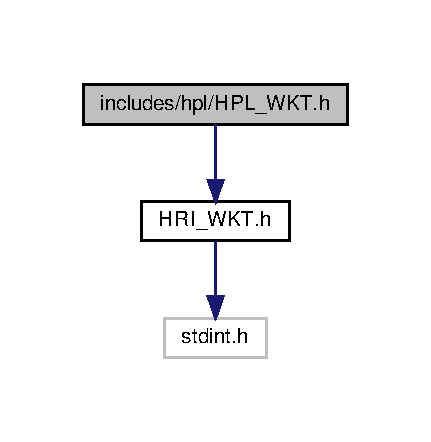
\includegraphics[width=207pt]{d1/db0/HPL__WKT_8h__incl}
\end{center}
\end{figure}
Gráfico de los archivos que directa o indirectamente incluyen a este archivo\+:\nopagebreak
\begin{figure}[H]
\begin{center}
\leavevmode
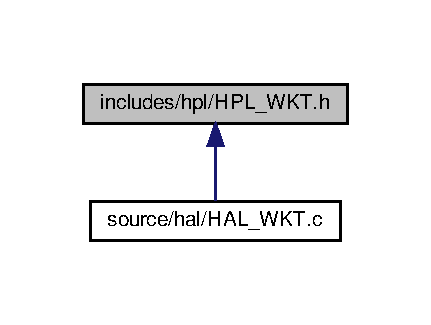
\includegraphics[width=207pt]{db/d59/HPL__WKT_8h__dep__incl}
\end{center}
\end{figure}
\subsection*{Enumeraciones}
\begin{DoxyCompactItemize}
\item 
\mbox{\Hypertarget{HPL__WKT_8h_ae456b8f1d9b852f9509b7e489bed02cc}\label{HPL__WKT_8h_ae456b8f1d9b852f9509b7e489bed02cc}} 
enum {\bfseries W\+K\+T\+\_\+clock\+\_\+source\+\_\+sel\+\_\+en} \{ {\bfseries W\+K\+T\+\_\+\+C\+L\+O\+C\+K\+\_\+\+S\+O\+U\+R\+C\+E\+\_\+\+D\+I\+V\+I\+D\+E\+D\+\_\+\+F\+RO} = 0, 
{\bfseries W\+K\+T\+\_\+\+C\+L\+O\+C\+K\+\_\+\+S\+O\+U\+R\+C\+E\+\_\+\+L\+O\+W\+\_\+\+P\+O\+W\+E\+R\+\_\+\+C\+L\+O\+CK}
 \}
\end{DoxyCompactItemize}
\subsection*{Funciones}
\begin{DoxyCompactItemize}
\item 
static void \hyperlink{HPL__WKT_8h_a59660c681086f905ddfabeb3bb90d953}{W\+K\+T\+\_\+select\+\_\+clock\+\_\+source} (W\+K\+T\+\_\+clock\+\_\+source\+\_\+sel\+\_\+en clock\+\_\+source)
\begin{DoxyCompactList}\small\item\em Seleccionar la fuente de clock para el W\+KT. \end{DoxyCompactList}\item 
static uint8\+\_\+t \hyperlink{HPL__WKT_8h_a1435108dbd5da2c53854c9c2cd1b1061}{W\+K\+T\+\_\+get\+\_\+alarm\+\_\+flag} (void)
\begin{DoxyCompactList}\small\item\em Obtener flag de alarma actual. \end{DoxyCompactList}\item 
\mbox{\Hypertarget{HPL__WKT_8h_af90f50ed79fe1d17d50cde59b57b1a7e}\label{HPL__WKT_8h_af90f50ed79fe1d17d50cde59b57b1a7e}} 
static void \hyperlink{HPL__WKT_8h_af90f50ed79fe1d17d50cde59b57b1a7e}{W\+K\+T\+\_\+clear\+\_\+alarm\+\_\+flag} (void)
\begin{DoxyCompactList}\small\item\em Limpiar flag de alarma. \end{DoxyCompactList}\item 
\mbox{\Hypertarget{HPL__WKT_8h_a2e16565703bedf9275480fa1d64534e2}\label{HPL__WKT_8h_a2e16565703bedf9275480fa1d64534e2}} 
static void \hyperlink{HPL__WKT_8h_a2e16565703bedf9275480fa1d64534e2}{W\+K\+T\+\_\+clear\+\_\+count} (void)
\begin{DoxyCompactList}\small\item\em Limpiar el contador del W\+KT. \end{DoxyCompactList}\item 
\mbox{\Hypertarget{HPL__WKT_8h_a9549da312a2b86e2ff78432083db81ce}\label{HPL__WKT_8h_a9549da312a2b86e2ff78432083db81ce}} 
static void \hyperlink{HPL__WKT_8h_a9549da312a2b86e2ff78432083db81ce}{W\+K\+T\+\_\+set\+\_\+internal\+\_\+clock\+\_\+source} (void)
\begin{DoxyCompactList}\small\item\em Seleccionar fuente de clock interna para el W\+KT. \end{DoxyCompactList}\item 
\mbox{\Hypertarget{HPL__WKT_8h_ac5526894d4ad9204736110bcbf2e6806}\label{HPL__WKT_8h_ac5526894d4ad9204736110bcbf2e6806}} 
static void \hyperlink{HPL__WKT_8h_ac5526894d4ad9204736110bcbf2e6806}{W\+K\+T\+\_\+set\+\_\+external\+\_\+clock\+\_\+source} (void)
\begin{DoxyCompactList}\small\item\em Seleccionar fuente de clock externa para el W\+KT. \end{DoxyCompactList}\item 
static uint32\+\_\+t \hyperlink{HPL__WKT_8h_afac1767181620eaf57ec40df8d6beb73}{W\+K\+T\+\_\+get\+\_\+current\+\_\+count} (void)
\begin{DoxyCompactList}\small\item\em Obtener cuenta actual del W\+KT. \end{DoxyCompactList}\item 
static void \hyperlink{HPL__WKT_8h_aa2f253a81181546eec6682ad7955421a}{W\+K\+T\+\_\+write\+\_\+count} (uint32\+\_\+t count)
\begin{DoxyCompactList}\small\item\em Fijar la cuenta del W\+KT. \end{DoxyCompactList}\end{DoxyCompactItemize}
\subsection*{Variables}
\begin{DoxyCompactItemize}
\item 
\mbox{\Hypertarget{HPL__WKT_8h_a012b5af96d81b9da035789051c654c53}\label{HPL__WKT_8h_a012b5af96d81b9da035789051c654c53}} 
volatile \hyperlink{HRI__WKT_8h_d4/d9c/structWKT__per__t}{W\+K\+T\+\_\+per\+\_\+t} $\ast$const \hyperlink{HPL__WKT_8h_a012b5af96d81b9da035789051c654c53}{W\+KT}
\begin{DoxyCompactList}\small\item\em Periferico W\+KT. \end{DoxyCompactList}\end{DoxyCompactItemize}


\subsection{Descripción detallada}
Declaraciones a nivel de abstraccion de periferico del W\+KT (L\+P\+C845) 

\begin{DoxyAuthor}{Autor}
Augusto Santini 
\end{DoxyAuthor}
\begin{DoxyDate}{Fecha}
3/2020 
\end{DoxyDate}
\begin{DoxyVersion}{Versión}
1.\+0 
\end{DoxyVersion}


\subsection{Documentación de las funciones}
\mbox{\Hypertarget{HPL__WKT_8h_a59660c681086f905ddfabeb3bb90d953}\label{HPL__WKT_8h_a59660c681086f905ddfabeb3bb90d953}} 
\index{H\+P\+L\+\_\+\+W\+K\+T.\+h@{H\+P\+L\+\_\+\+W\+K\+T.\+h}!W\+K\+T\+\_\+select\+\_\+clock\+\_\+source@{W\+K\+T\+\_\+select\+\_\+clock\+\_\+source}}
\index{W\+K\+T\+\_\+select\+\_\+clock\+\_\+source@{W\+K\+T\+\_\+select\+\_\+clock\+\_\+source}!H\+P\+L\+\_\+\+W\+K\+T.\+h@{H\+P\+L\+\_\+\+W\+K\+T.\+h}}
\subsubsection{\texorpdfstring{W\+K\+T\+\_\+select\+\_\+clock\+\_\+source()}{WKT\_select\_clock\_source()}}
{\footnotesize\ttfamily static void W\+K\+T\+\_\+select\+\_\+clock\+\_\+source (\begin{DoxyParamCaption}\item[{W\+K\+T\+\_\+clock\+\_\+source\+\_\+sel\+\_\+en}]{clock\+\_\+source }\end{DoxyParamCaption})\hspace{0.3cm}{\ttfamily [inline]}, {\ttfamily [static]}}



Seleccionar la fuente de clock para el W\+KT. 


\begin{DoxyParams}[1]{Parámetros}
\mbox{\tt in}  & {\em clock\+\_\+source} & Fuente de clock deseada \\
\hline
\end{DoxyParams}
\mbox{\Hypertarget{HPL__WKT_8h_a1435108dbd5da2c53854c9c2cd1b1061}\label{HPL__WKT_8h_a1435108dbd5da2c53854c9c2cd1b1061}} 
\index{H\+P\+L\+\_\+\+W\+K\+T.\+h@{H\+P\+L\+\_\+\+W\+K\+T.\+h}!W\+K\+T\+\_\+get\+\_\+alarm\+\_\+flag@{W\+K\+T\+\_\+get\+\_\+alarm\+\_\+flag}}
\index{W\+K\+T\+\_\+get\+\_\+alarm\+\_\+flag@{W\+K\+T\+\_\+get\+\_\+alarm\+\_\+flag}!H\+P\+L\+\_\+\+W\+K\+T.\+h@{H\+P\+L\+\_\+\+W\+K\+T.\+h}}
\subsubsection{\texorpdfstring{W\+K\+T\+\_\+get\+\_\+alarm\+\_\+flag()}{WKT\_get\_alarm\_flag()}}
{\footnotesize\ttfamily static uint8\+\_\+t W\+K\+T\+\_\+get\+\_\+alarm\+\_\+flag (\begin{DoxyParamCaption}\item[{void}]{ }\end{DoxyParamCaption})\hspace{0.3cm}{\ttfamily [inline]}, {\ttfamily [static]}}



Obtener flag de alarma actual. 

\begin{DoxyReturn}{Devuelve}
Estado del flag de alarma actual 
\end{DoxyReturn}
\mbox{\Hypertarget{HPL__WKT_8h_afac1767181620eaf57ec40df8d6beb73}\label{HPL__WKT_8h_afac1767181620eaf57ec40df8d6beb73}} 
\index{H\+P\+L\+\_\+\+W\+K\+T.\+h@{H\+P\+L\+\_\+\+W\+K\+T.\+h}!W\+K\+T\+\_\+get\+\_\+current\+\_\+count@{W\+K\+T\+\_\+get\+\_\+current\+\_\+count}}
\index{W\+K\+T\+\_\+get\+\_\+current\+\_\+count@{W\+K\+T\+\_\+get\+\_\+current\+\_\+count}!H\+P\+L\+\_\+\+W\+K\+T.\+h@{H\+P\+L\+\_\+\+W\+K\+T.\+h}}
\subsubsection{\texorpdfstring{W\+K\+T\+\_\+get\+\_\+current\+\_\+count()}{WKT\_get\_current\_count()}}
{\footnotesize\ttfamily static uint32\+\_\+t W\+K\+T\+\_\+get\+\_\+current\+\_\+count (\begin{DoxyParamCaption}\item[{void}]{ }\end{DoxyParamCaption})\hspace{0.3cm}{\ttfamily [inline]}, {\ttfamily [static]}}



Obtener cuenta actual del W\+KT. 

\begin{DoxyReturn}{Devuelve}
Cuenta actual del W\+KT 
\end{DoxyReturn}
\mbox{\Hypertarget{HPL__WKT_8h_aa2f253a81181546eec6682ad7955421a}\label{HPL__WKT_8h_aa2f253a81181546eec6682ad7955421a}} 
\index{H\+P\+L\+\_\+\+W\+K\+T.\+h@{H\+P\+L\+\_\+\+W\+K\+T.\+h}!W\+K\+T\+\_\+write\+\_\+count@{W\+K\+T\+\_\+write\+\_\+count}}
\index{W\+K\+T\+\_\+write\+\_\+count@{W\+K\+T\+\_\+write\+\_\+count}!H\+P\+L\+\_\+\+W\+K\+T.\+h@{H\+P\+L\+\_\+\+W\+K\+T.\+h}}
\subsubsection{\texorpdfstring{W\+K\+T\+\_\+write\+\_\+count()}{WKT\_write\_count()}}
{\footnotesize\ttfamily static void W\+K\+T\+\_\+write\+\_\+count (\begin{DoxyParamCaption}\item[{uint32\+\_\+t}]{count }\end{DoxyParamCaption})\hspace{0.3cm}{\ttfamily [inline]}, {\ttfamily [static]}}



Fijar la cuenta del W\+KT. 


\begin{DoxyParams}[1]{Parámetros}
\mbox{\tt in}  & {\em count} & Valor de cuenta deseado \\
\hline
\end{DoxyParams}

\hypertarget{HRI__ADC_8h}{}\section{Referencia del Archivo includes/hri/\+H\+R\+I\+\_\+\+A\+DC.h}
\label{HRI__ADC_8h}\index{includes/hri/\+H\+R\+I\+\_\+\+A\+D\+C.\+h@{includes/hri/\+H\+R\+I\+\_\+\+A\+D\+C.\+h}}


Declaraciones a nivel de registros del A\+DC (L\+P\+C845)  


{\ttfamily \#include $<$stdint.\+h$>$}\newline
Dependencia gráfica adjunta para H\+R\+I\+\_\+\+A\+D\+C.\+h\+:\nopagebreak
\begin{figure}[H]
\begin{center}
\leavevmode
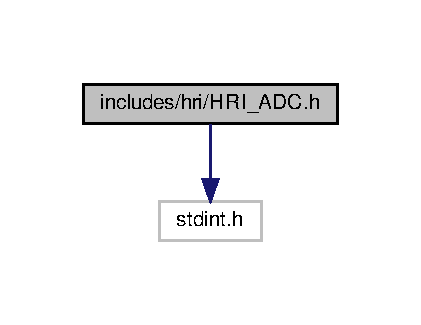
\includegraphics[width=202pt]{HRI__ADC_8h__incl}
\end{center}
\end{figure}
Gráfico de los archivos que directa o indirectamente incluyen a este archivo\+:\nopagebreak
\begin{figure}[H]
\begin{center}
\leavevmode
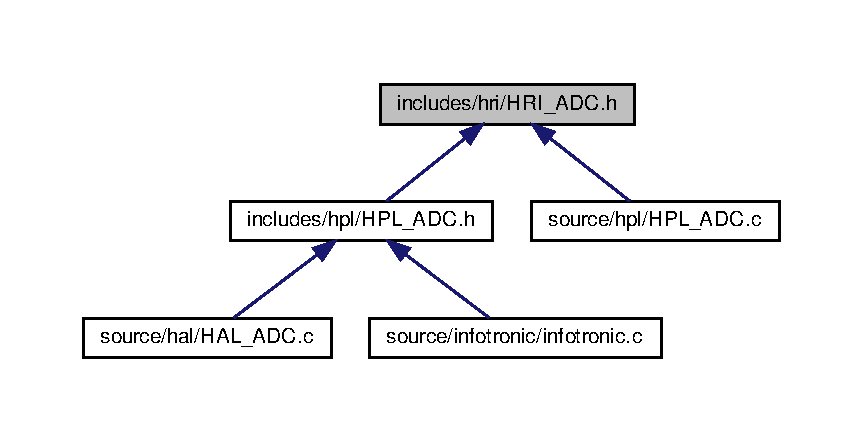
\includegraphics[width=350pt]{HRI__ADC_8h__dep__incl}
\end{center}
\end{figure}
\subsection*{Estructuras de datos}
\begin{DoxyCompactItemize}
\item 
struct \hyperlink{HRI__ADC_8h_structADC__CTRL__reg__t}{A\+D\+C\+\_\+\+C\+T\+R\+L\+\_\+reg\+\_\+t}
\begin{DoxyCompactList}\small\item\em Registro de control del A\+DC.  \hyperlink{HRI__ADC_8h_structADC__CTRL__reg__t}{Más...}\end{DoxyCompactList}\item 
struct \hyperlink{HRI__ADC_8h_structADC__SEQ__CTRL__reg__t}{A\+D\+C\+\_\+\+S\+E\+Q\+\_\+\+C\+T\+R\+L\+\_\+reg\+\_\+t}
\begin{DoxyCompactList}\small\item\em Registro de control de secuencia A y B del A\+DC.  \hyperlink{HRI__ADC_8h_structADC__SEQ__CTRL__reg__t}{Más...}\end{DoxyCompactList}\item 
struct \hyperlink{HRI__ADC_8h_structADC__SEQ__GDAT__reg__t}{A\+D\+C\+\_\+\+S\+E\+Q\+\_\+\+G\+D\+A\+T\+\_\+reg\+\_\+t}
\item 
struct \hyperlink{HRI__ADC_8h_structADC__DAT__reg__t}{A\+D\+C\+\_\+\+D\+A\+T\+\_\+reg\+\_\+t}
\item 
struct \hyperlink{HRI__ADC_8h_structADC__THR__LOW__reg__t}{A\+D\+C\+\_\+\+T\+H\+R\+\_\+\+L\+O\+W\+\_\+reg\+\_\+t}
\item 
struct \hyperlink{HRI__ADC_8h_structADC__THR__HIGH__reg__t}{A\+D\+C\+\_\+\+T\+H\+R\+\_\+\+H\+I\+G\+H\+\_\+reg\+\_\+t}
\item 
struct \hyperlink{HRI__ADC_8h_structADC__CHAN__THRSEL__reg__t}{A\+D\+C\+\_\+\+C\+H\+A\+N\+\_\+\+T\+H\+R\+S\+E\+L\+\_\+reg\+\_\+t}
\item 
struct \hyperlink{HRI__ADC_8h_structADC__INTEN__reg__t}{A\+D\+C\+\_\+\+I\+N\+T\+E\+N\+\_\+reg\+\_\+t}
\item 
struct \hyperlink{HRI__ADC_8h_structADC__FLAGS__reg__t}{A\+D\+C\+\_\+\+F\+L\+A\+G\+S\+\_\+reg\+\_\+t}
\item 
struct \hyperlink{HRI__ADC_8h_structADC__TRM__reg__t}{A\+D\+C\+\_\+\+T\+R\+M\+\_\+reg\+\_\+t}
\item 
struct \hyperlink{HRI__ADC_8h_structADC__per__t}{A\+D\+C\+\_\+per\+\_\+t}
\end{DoxyCompactItemize}
\subsection*{defines}
\begin{DoxyCompactItemize}
\item 
\mbox{\Hypertarget{HRI__ADC_8h_ad06cb9e5985bd216a376f26f22303cd6}\label{HRI__ADC_8h_ad06cb9e5985bd216a376f26f22303cd6}} 
\#define \hyperlink{HRI__ADC_8h_ad06cb9e5985bd216a376f26f22303cd6}{A\+D\+C\+\_\+\+B\+A\+SE}~0x4001\+C000
\begin{DoxyCompactList}\small\item\em Direccion base del A\+DC. \end{DoxyCompactList}\end{DoxyCompactItemize}


\subsection{Descripción detallada}
Declaraciones a nivel de registros del A\+DC (L\+P\+C845) 

\begin{DoxyAuthor}{Autor}
Augusto Santini 
\end{DoxyAuthor}
\begin{DoxyDate}{Fecha}
6/2019 
\end{DoxyDate}
\begin{DoxyVersion}{Versión}
1.\+0 
\end{DoxyVersion}


\subsection{Documentación de las estructuras de datos}
\index{A\+D\+C\+\_\+\+C\+T\+R\+L\+\_\+reg\+\_\+t@{A\+D\+C\+\_\+\+C\+T\+R\+L\+\_\+reg\+\_\+t}}\label{structADC__CTRL__reg__t}
\Hypertarget{HRI__ADC_8h_structADC__CTRL__reg__t}
\subsubsection{struct A\+D\+C\+\_\+\+C\+T\+R\+L\+\_\+reg\+\_\+t}
Registro de control del A\+DC. \begin{DoxyFields}{Campos de datos}
\mbox{\Hypertarget{HRI__ADC_8h_aa11dafc1481a6f613e960f2a7a83db4c}\label{HRI__ADC_8h_aa11dafc1481a6f613e960f2a7a83db4c}} 
uint32\_t&
CLKDIV: 8&
Divisor del clock. \\
\hline

\mbox{\Hypertarget{HRI__ADC_8h_a5e26c94dd1953ec73e4163f0b135ae24}\label{HRI__ADC_8h_a5e26c94dd1953ec73e4163f0b135ae24}} 
uint32\_t&
ASYNCMODE: 1&
0 -\/$>$ Modo sincronico ; 1 -\/$>$ Modo asincronico \\
\hline

\mbox{\Hypertarget{HRI__ADC_8h_a25005b5a2bb3bc40be61ed867476e954}\label{HRI__ADC_8h_a25005b5a2bb3bc40be61ed867476e954}} 
uint32\_t&
\_\_pad0\_\_: 1&
Reservado. \\
\hline

\mbox{\Hypertarget{HRI__ADC_8h_ac7ad855f464226b05393c01215077633}\label{HRI__ADC_8h_ac7ad855f464226b05393c01215077633}} 
uint32\_t&
LPWRMODE: 1&
Modo de bajo consumo. \\
\hline

\mbox{\Hypertarget{HRI__ADC_8h_a102f9e809bada5e43d0aea84f8a41874}\label{HRI__ADC_8h_a102f9e809bada5e43d0aea84f8a41874}} 
uint32\_t&
\_\_pad1\_\_: 19&
Reservado. \\
\hline

\mbox{\Hypertarget{HRI__ADC_8h_add69b74ced19a7667ec73b713dc9dfae}\label{HRI__ADC_8h_add69b74ced19a7667ec73b713dc9dfae}} 
uint32\_t&
CALMODE: 1&
Modo calibracion. \\
\hline

\mbox{\Hypertarget{HRI__ADC_8h_ad5e2f85196dc5cef7a906d8db3b5fd08}\label{HRI__ADC_8h_ad5e2f85196dc5cef7a906d8db3b5fd08}} 
uint32\_t&
\_\_pad2\_\_: 1&
Reservado. \\
\hline

\end{DoxyFields}
\index{A\+D\+C\+\_\+\+S\+E\+Q\+\_\+\+C\+T\+R\+L\+\_\+reg\+\_\+t@{A\+D\+C\+\_\+\+S\+E\+Q\+\_\+\+C\+T\+R\+L\+\_\+reg\+\_\+t}}\label{structADC__SEQ__CTRL__reg__t}
\Hypertarget{HRI__ADC_8h_structADC__SEQ__CTRL__reg__t}
\subsubsection{struct A\+D\+C\+\_\+\+S\+E\+Q\+\_\+\+C\+T\+R\+L\+\_\+reg\+\_\+t}
Registro de control de secuencia A y B del A\+DC. \begin{DoxyFields}{Campos de datos}
\mbox{\Hypertarget{HRI__ADC_8h_ab6b7040c8266731e8b3759ccb41b181d}\label{HRI__ADC_8h_ab6b7040c8266731e8b3759ccb41b181d}} 
uint32\_t&
CHANNELS: 12&
Canales habilitados para la conversion en la secuencia. \\
\hline

\mbox{\Hypertarget{HRI__ADC_8h_a084459dd951ce06483ea9fb3cb1d8c9c}\label{HRI__ADC_8h_a084459dd951ce06483ea9fb3cb1d8c9c}} 
uint32\_t&
TRIGGER: 3&
Que pin dispara la secuencia. \\
\hline

\mbox{\Hypertarget{HRI__ADC_8h_a721419bb352a88096d7e1e78b2a33546}\label{HRI__ADC_8h_a721419bb352a88096d7e1e78b2a33546}} 
uint32\_t&
\_\_pad0\_\_: 3&
Reservado. \\
\hline

\mbox{\Hypertarget{HRI__ADC_8h_a650a87293bd0fae1cae6f3516d6c8b2a}\label{HRI__ADC_8h_a650a87293bd0fae1cae6f3516d6c8b2a}} 
uint32\_t&
TRIGPOL: 1&
Polaridad del pin que dispara la secuencia. \\
\hline

\mbox{\Hypertarget{HRI__ADC_8h_a9cd98dfe9fef83393cc3444269a789b6}\label{HRI__ADC_8h_a9cd98dfe9fef83393cc3444269a789b6}} 
uint32\_t&
SYNCBYPASS: 1&
Disparo asincronico/sincronico. \\
\hline

\mbox{\Hypertarget{HRI__ADC_8h_a576aaa829a04bc01cf40b1d1518d3b14}\label{HRI__ADC_8h_a576aaa829a04bc01cf40b1d1518d3b14}} 
uint32\_t&
\_\_pad1\_\_: 6&
Reservado. \\
\hline

\mbox{\Hypertarget{HRI__ADC_8h_aa88a104386674129a3e562cb0d90dd43}\label{HRI__ADC_8h_aa88a104386674129a3e562cb0d90dd43}} 
uint32\_t&
START: 1&
Empezar secuencia mediante software. \\
\hline

\mbox{\Hypertarget{HRI__ADC_8h_a6b54386ca3acc9f6976d71116e0eb1ae}\label{HRI__ADC_8h_a6b54386ca3acc9f6976d71116e0eb1ae}} 
uint32\_t&
BURST: 1&
Habilitacion de modo rafaga. \\
\hline

\mbox{\Hypertarget{HRI__ADC_8h_a7483a428267e32f221ca15513e399351}\label{HRI__ADC_8h_a7483a428267e32f221ca15513e399351}} 
uint32\_t&
SINGLESTEP: 1&
Un start activa un paso o la secuencia entera. \\
\hline

\mbox{\Hypertarget{HRI__ADC_8h_ac32d66a04cd04d1fc9188eebd52dcbbb}\label{HRI__ADC_8h_ac32d66a04cd04d1fc9188eebd52dcbbb}} 
uint32\_t&
LOWPRIO: 1&
Prioridad. Solo lo tiene la secuencia A. \\
\hline

\mbox{\Hypertarget{HRI__ADC_8h_a0d37f1cfd8da2630136984b1df1406c0}\label{HRI__ADC_8h_a0d37f1cfd8da2630136984b1df1406c0}} 
uint32\_t&
MODE: 1&
Interrupcion por cada conversion o al final de la secuencia. \\
\hline

\mbox{\Hypertarget{HRI__ADC_8h_af3cb32440527b1a981821556c861d3c6}\label{HRI__ADC_8h_af3cb32440527b1a981821556c861d3c6}} 
uint32\_t&
SEQ\_ENA: 1&
Habilitacion de secuencia. \\
\hline

\end{DoxyFields}
\index{A\+D\+C\+\_\+\+S\+E\+Q\+\_\+\+G\+D\+A\+T\+\_\+reg\+\_\+t@{A\+D\+C\+\_\+\+S\+E\+Q\+\_\+\+G\+D\+A\+T\+\_\+reg\+\_\+t}}\label{structADC__SEQ__GDAT__reg__t}
\Hypertarget{HRI__ADC_8h_structADC__SEQ__GDAT__reg__t}
\subsubsection{struct A\+D\+C\+\_\+\+S\+E\+Q\+\_\+\+G\+D\+A\+T\+\_\+reg\+\_\+t}
\begin{DoxyFields}{Campos de datos}
\mbox{\Hypertarget{HRI__ADC_8h_a2f56e5280450eb38fa40ee724337c7a5}\label{HRI__ADC_8h_a2f56e5280450eb38fa40ee724337c7a5}} 
uint32\_t&
\_\_pad0\_\_: 4&
\\
\hline

\mbox{\Hypertarget{HRI__ADC_8h_a2c6c1bca893df8daa705d0f33a1a1d4a}\label{HRI__ADC_8h_a2c6c1bca893df8daa705d0f33a1a1d4a}} 
uint32\_t&
RESULT: 12&
\\
\hline

\mbox{\Hypertarget{HRI__ADC_8h_ab8df862a572124b019a973aa04356e4f}\label{HRI__ADC_8h_ab8df862a572124b019a973aa04356e4f}} 
uint32\_t&
THCMPRANGE: 2&
\\
\hline

\mbox{\Hypertarget{HRI__ADC_8h_a3b48ee95e4be244fb36d467d0860a887}\label{HRI__ADC_8h_a3b48ee95e4be244fb36d467d0860a887}} 
uint32\_t&
THCMPCROSS: 2&
\\
\hline

\mbox{\Hypertarget{HRI__ADC_8h_a4fffa23c0b8fe680214ccf5f39525d76}\label{HRI__ADC_8h_a4fffa23c0b8fe680214ccf5f39525d76}} 
uint32\_t&
\_\_pad1\_\_: 6&
\\
\hline

\mbox{\Hypertarget{HRI__ADC_8h_a3ad04b3815d4d6361f6eae2188bc22c2}\label{HRI__ADC_8h_a3ad04b3815d4d6361f6eae2188bc22c2}} 
uint32\_t&
CHANNEL: 4&
\\
\hline

\mbox{\Hypertarget{HRI__ADC_8h_a38c1e51738a727e75d4779f1892228c4}\label{HRI__ADC_8h_a38c1e51738a727e75d4779f1892228c4}} 
uint32\_t&
OVERRUN: 1&
\\
\hline

\mbox{\Hypertarget{HRI__ADC_8h_a7cf0dcfd5dc654a931b6f8005515b65d}\label{HRI__ADC_8h_a7cf0dcfd5dc654a931b6f8005515b65d}} 
uint32\_t&
DATAVALID: 1&
\\
\hline

\end{DoxyFields}
\index{A\+D\+C\+\_\+\+D\+A\+T\+\_\+reg\+\_\+t@{A\+D\+C\+\_\+\+D\+A\+T\+\_\+reg\+\_\+t}}\label{structADC__DAT__reg__t}
\Hypertarget{HRI__ADC_8h_structADC__DAT__reg__t}
\subsubsection{struct A\+D\+C\+\_\+\+D\+A\+T\+\_\+reg\+\_\+t}
\begin{DoxyFields}{Campos de datos}
\mbox{\Hypertarget{HRI__ADC_8h_a8f920caf1aa0db0cfbad8adfaaf0a2ea}\label{HRI__ADC_8h_a8f920caf1aa0db0cfbad8adfaaf0a2ea}} 
uint32\_t&
\_\_pad0\_\_: 4&
\\
\hline

\mbox{\Hypertarget{HRI__ADC_8h_a0adfc8b45e8a5f696d64762a7c5653f2}\label{HRI__ADC_8h_a0adfc8b45e8a5f696d64762a7c5653f2}} 
uint32\_t&
RESULT: 12&
\\
\hline

\mbox{\Hypertarget{HRI__ADC_8h_abaaaca8f45f89a9564fc142d8795deff}\label{HRI__ADC_8h_abaaaca8f45f89a9564fc142d8795deff}} 
uint32\_t&
THCMPRANGE: 2&
\\
\hline

\mbox{\Hypertarget{HRI__ADC_8h_a74cd3e307708950cb8d109ff623382bd}\label{HRI__ADC_8h_a74cd3e307708950cb8d109ff623382bd}} 
uint32\_t&
THCMPCROSS: 2&
\\
\hline

\mbox{\Hypertarget{HRI__ADC_8h_a4fde7c54e264ea9b75f92d8252d3e04f}\label{HRI__ADC_8h_a4fde7c54e264ea9b75f92d8252d3e04f}} 
uint32\_t&
\_\_pad1\_\_: 6&
\\
\hline

\mbox{\Hypertarget{HRI__ADC_8h_adefcf47eff6ede66de28004b33106a9c}\label{HRI__ADC_8h_adefcf47eff6ede66de28004b33106a9c}} 
uint32\_t&
CHANNEL: 4&
\\
\hline

\mbox{\Hypertarget{HRI__ADC_8h_a77ab85598eb2b6fb7205aeebb9ab5724}\label{HRI__ADC_8h_a77ab85598eb2b6fb7205aeebb9ab5724}} 
uint32\_t&
OVERRUN: 1&
\\
\hline

\mbox{\Hypertarget{HRI__ADC_8h_aab1522c4774195c5ad3a6ce50ba08c9a}\label{HRI__ADC_8h_aab1522c4774195c5ad3a6ce50ba08c9a}} 
uint32\_t&
DATAVALID: 1&
\\
\hline

\end{DoxyFields}
\index{A\+D\+C\+\_\+\+T\+H\+R\+\_\+\+L\+O\+W\+\_\+reg\+\_\+t@{A\+D\+C\+\_\+\+T\+H\+R\+\_\+\+L\+O\+W\+\_\+reg\+\_\+t}}\label{structADC__THR__LOW__reg__t}
\Hypertarget{HRI__ADC_8h_structADC__THR__LOW__reg__t}
\subsubsection{struct A\+D\+C\+\_\+\+T\+H\+R\+\_\+\+L\+O\+W\+\_\+reg\+\_\+t}
\begin{DoxyFields}{Campos de datos}
\mbox{\Hypertarget{HRI__ADC_8h_a568e8578c21ed17b0251f87333fb40f8}\label{HRI__ADC_8h_a568e8578c21ed17b0251f87333fb40f8}} 
uint32\_t&
\_\_pad0\_\_: 4&
\\
\hline

\mbox{\Hypertarget{HRI__ADC_8h_a8207b6021b9929e9fec13666cb72e344}\label{HRI__ADC_8h_a8207b6021b9929e9fec13666cb72e344}} 
uint32\_t&
THRLOW: 12&
\\
\hline

\mbox{\Hypertarget{HRI__ADC_8h_a847d59ad91219f4fff46a1f41dd7e397}\label{HRI__ADC_8h_a847d59ad91219f4fff46a1f41dd7e397}} 
uint32\_t&
\_\_pad1\_\_: 16&
\\
\hline

\end{DoxyFields}
\index{A\+D\+C\+\_\+\+T\+H\+R\+\_\+\+H\+I\+G\+H\+\_\+reg\+\_\+t@{A\+D\+C\+\_\+\+T\+H\+R\+\_\+\+H\+I\+G\+H\+\_\+reg\+\_\+t}}\label{structADC__THR__HIGH__reg__t}
\Hypertarget{HRI__ADC_8h_structADC__THR__HIGH__reg__t}
\subsubsection{struct A\+D\+C\+\_\+\+T\+H\+R\+\_\+\+H\+I\+G\+H\+\_\+reg\+\_\+t}
\begin{DoxyFields}{Campos de datos}
\mbox{\Hypertarget{HRI__ADC_8h_aa826bfd2bcf0702a8227272623399533}\label{HRI__ADC_8h_aa826bfd2bcf0702a8227272623399533}} 
uint32\_t&
\_\_pad0\_\_: 4&
\\
\hline

\mbox{\Hypertarget{HRI__ADC_8h_ab85de0f9b2144149bec70111098413a2}\label{HRI__ADC_8h_ab85de0f9b2144149bec70111098413a2}} 
uint32\_t&
THRHIGH: 12&
\\
\hline

\mbox{\Hypertarget{HRI__ADC_8h_a600b63b1a046459bdbfb86d1e4a180b5}\label{HRI__ADC_8h_a600b63b1a046459bdbfb86d1e4a180b5}} 
uint32\_t&
\_\_pad1\_\_: 16&
\\
\hline

\end{DoxyFields}
\index{A\+D\+C\+\_\+\+C\+H\+A\+N\+\_\+\+T\+H\+R\+S\+E\+L\+\_\+reg\+\_\+t@{A\+D\+C\+\_\+\+C\+H\+A\+N\+\_\+\+T\+H\+R\+S\+E\+L\+\_\+reg\+\_\+t}}\label{structADC__CHAN__THRSEL__reg__t}
\Hypertarget{HRI__ADC_8h_structADC__CHAN__THRSEL__reg__t}
\subsubsection{struct A\+D\+C\+\_\+\+C\+H\+A\+N\+\_\+\+T\+H\+R\+S\+E\+L\+\_\+reg\+\_\+t}
\begin{DoxyFields}{Campos de datos}
\mbox{\Hypertarget{HRI__ADC_8h_a14a400128b8b185d4d50ab15c53662dd}\label{HRI__ADC_8h_a14a400128b8b185d4d50ab15c53662dd}} 
uint32\_t&
CH0\_THRSEL: 1&
\\
\hline

\mbox{\Hypertarget{HRI__ADC_8h_abe8eb3a1076fa59fb076ad308d512ca4}\label{HRI__ADC_8h_abe8eb3a1076fa59fb076ad308d512ca4}} 
uint32\_t&
CH1\_THRSEL: 1&
\\
\hline

\mbox{\Hypertarget{HRI__ADC_8h_a1bef171d780cdded2c2fe1ef96dd201d}\label{HRI__ADC_8h_a1bef171d780cdded2c2fe1ef96dd201d}} 
uint32\_t&
CH2\_THRSEL: 1&
\\
\hline

\mbox{\Hypertarget{HRI__ADC_8h_a4a43cc8354ea3c8a06f622fa69d8265f}\label{HRI__ADC_8h_a4a43cc8354ea3c8a06f622fa69d8265f}} 
uint32\_t&
CH3\_THRSEL: 1&
\\
\hline

\mbox{\Hypertarget{HRI__ADC_8h_a10fe7e0c3f47a80708ff210b88646d82}\label{HRI__ADC_8h_a10fe7e0c3f47a80708ff210b88646d82}} 
uint32\_t&
CH4\_THRSEL: 1&
\\
\hline

\mbox{\Hypertarget{HRI__ADC_8h_a1d2f13e1443255163934aeb454a122dc}\label{HRI__ADC_8h_a1d2f13e1443255163934aeb454a122dc}} 
uint32\_t&
CH5\_THRSEL: 1&
\\
\hline

\mbox{\Hypertarget{HRI__ADC_8h_aaee6419a74514518133573573ba46724}\label{HRI__ADC_8h_aaee6419a74514518133573573ba46724}} 
uint32\_t&
CH6\_THRSEL: 1&
\\
\hline

\mbox{\Hypertarget{HRI__ADC_8h_a367354074768315577f2d6b7ba773f63}\label{HRI__ADC_8h_a367354074768315577f2d6b7ba773f63}} 
uint32\_t&
CH7\_THRSEL: 1&
\\
\hline

\mbox{\Hypertarget{HRI__ADC_8h_ae02e0c899ef1f2f76cf99b0d879df29d}\label{HRI__ADC_8h_ae02e0c899ef1f2f76cf99b0d879df29d}} 
uint32\_t&
CH8\_THRSEL: 1&
\\
\hline

\mbox{\Hypertarget{HRI__ADC_8h_aa4b26060a39c1806a41c7d648842d39c}\label{HRI__ADC_8h_aa4b26060a39c1806a41c7d648842d39c}} 
uint32\_t&
CH9\_THRSEL: 1&
\\
\hline

\mbox{\Hypertarget{HRI__ADC_8h_a647ef31fb9517be44c61f15b70925122}\label{HRI__ADC_8h_a647ef31fb9517be44c61f15b70925122}} 
uint32\_t&
CH10\_THRSEL: 1&
\\
\hline

\mbox{\Hypertarget{HRI__ADC_8h_a1e12df9df2514228f3bb3dd2b6043be9}\label{HRI__ADC_8h_a1e12df9df2514228f3bb3dd2b6043be9}} 
uint32\_t&
CH11\_THRSEL: 1&
\\
\hline

\mbox{\Hypertarget{HRI__ADC_8h_af8f53e5b8a6ab35a32804c415097e622}\label{HRI__ADC_8h_af8f53e5b8a6ab35a32804c415097e622}} 
uint32\_t&
\_\_pad0\_\_: 20&
\\
\hline

\end{DoxyFields}
\index{A\+D\+C\+\_\+\+I\+N\+T\+E\+N\+\_\+reg\+\_\+t@{A\+D\+C\+\_\+\+I\+N\+T\+E\+N\+\_\+reg\+\_\+t}}\label{structADC__INTEN__reg__t}
\Hypertarget{HRI__ADC_8h_structADC__INTEN__reg__t}
\subsubsection{struct A\+D\+C\+\_\+\+I\+N\+T\+E\+N\+\_\+reg\+\_\+t}
\begin{DoxyFields}{Campos de datos}
\mbox{\Hypertarget{HRI__ADC_8h_a0f319568c0d12c7e914111b58b53ac28}\label{HRI__ADC_8h_a0f319568c0d12c7e914111b58b53ac28}} 
uint32\_t&
SEQA\_INTEN: 1&
\\
\hline

\mbox{\Hypertarget{HRI__ADC_8h_af146705edee27ea36a37e61f5fd7221e}\label{HRI__ADC_8h_af146705edee27ea36a37e61f5fd7221e}} 
uint32\_t&
SEQB\_INTEN: 1&
\\
\hline

\mbox{\Hypertarget{HRI__ADC_8h_a675e583fa52a9eac076cdd96da009797}\label{HRI__ADC_8h_a675e583fa52a9eac076cdd96da009797}} 
uint32\_t&
OVR\_INTEN: 1&
\\
\hline

\mbox{\Hypertarget{HRI__ADC_8h_a7be989eb8f7661e35013c858b2a6a8c5}\label{HRI__ADC_8h_a7be989eb8f7661e35013c858b2a6a8c5}} 
uint32\_t&
ADCMPINTEN0: 2&
\\
\hline

\mbox{\Hypertarget{HRI__ADC_8h_aa02ae2c717ed2e78efeb51a3b541a877}\label{HRI__ADC_8h_aa02ae2c717ed2e78efeb51a3b541a877}} 
uint32\_t&
ADCMPINTEN1: 2&
\\
\hline

\mbox{\Hypertarget{HRI__ADC_8h_a8cbca9773ea0ff462cc3e84bdc28763c}\label{HRI__ADC_8h_a8cbca9773ea0ff462cc3e84bdc28763c}} 
uint32\_t&
ADCMPINTEN2: 2&
\\
\hline

\mbox{\Hypertarget{HRI__ADC_8h_a756b204f8193464e34bad4167d547bfb}\label{HRI__ADC_8h_a756b204f8193464e34bad4167d547bfb}} 
uint32\_t&
ADCMPINTEN3: 2&
\\
\hline

\mbox{\Hypertarget{HRI__ADC_8h_a4093896d892099eee00eab9f2965682a}\label{HRI__ADC_8h_a4093896d892099eee00eab9f2965682a}} 
uint32\_t&
ADCMPINTEN4: 2&
\\
\hline

\mbox{\Hypertarget{HRI__ADC_8h_aa95ae03000f0b4f7fd80d672e6c62610}\label{HRI__ADC_8h_aa95ae03000f0b4f7fd80d672e6c62610}} 
uint32\_t&
ADCMPINTEN5: 2&
\\
\hline

\mbox{\Hypertarget{HRI__ADC_8h_af48a4b3bc2a2e08b2f3db2d17d33a6cf}\label{HRI__ADC_8h_af48a4b3bc2a2e08b2f3db2d17d33a6cf}} 
uint32\_t&
ADCMPINTEN6: 2&
\\
\hline

\mbox{\Hypertarget{HRI__ADC_8h_a0158844decca53fa58f52038d150983a}\label{HRI__ADC_8h_a0158844decca53fa58f52038d150983a}} 
uint32\_t&
ADCMPINTEN7: 2&
\\
\hline

\mbox{\Hypertarget{HRI__ADC_8h_ad80e2bc403575c3f9b95dcc508a82afa}\label{HRI__ADC_8h_ad80e2bc403575c3f9b95dcc508a82afa}} 
uint32\_t&
ADCMPINTEN8: 2&
\\
\hline

\mbox{\Hypertarget{HRI__ADC_8h_aa46db5b030d36563f2ab280d9b0ed005}\label{HRI__ADC_8h_aa46db5b030d36563f2ab280d9b0ed005}} 
uint32\_t&
ADCMPINTEN9: 2&
\\
\hline

\mbox{\Hypertarget{HRI__ADC_8h_afc8946df8dd6b2279b31a513a63a99a6}\label{HRI__ADC_8h_afc8946df8dd6b2279b31a513a63a99a6}} 
uint32\_t&
ADCMPINTEN10: 2&
\\
\hline

\mbox{\Hypertarget{HRI__ADC_8h_a09833b8f75225408e5691a42026aad74}\label{HRI__ADC_8h_a09833b8f75225408e5691a42026aad74}} 
uint32\_t&
ADCMPINTEN11: 2&
\\
\hline

\mbox{\Hypertarget{HRI__ADC_8h_a51c88bc2e9b17f10d7f23cd4a0c0d88a}\label{HRI__ADC_8h_a51c88bc2e9b17f10d7f23cd4a0c0d88a}} 
uint32\_t&
\_\_pad0\_\_: 5&
\\
\hline

\end{DoxyFields}
\index{A\+D\+C\+\_\+\+F\+L\+A\+G\+S\+\_\+reg\+\_\+t@{A\+D\+C\+\_\+\+F\+L\+A\+G\+S\+\_\+reg\+\_\+t}}\label{structADC__FLAGS__reg__t}
\Hypertarget{HRI__ADC_8h_structADC__FLAGS__reg__t}
\subsubsection{struct A\+D\+C\+\_\+\+F\+L\+A\+G\+S\+\_\+reg\+\_\+t}
\begin{DoxyFields}{Campos de datos}
\mbox{\Hypertarget{HRI__ADC_8h_a9b45e490adf8365e6b8ef67aea714399}\label{HRI__ADC_8h_a9b45e490adf8365e6b8ef67aea714399}} 
uint32\_t&
THCMP0: 1&
\\
\hline

\mbox{\Hypertarget{HRI__ADC_8h_a3175b65a1b5a0c3a3c993ad758ce5038}\label{HRI__ADC_8h_a3175b65a1b5a0c3a3c993ad758ce5038}} 
uint32\_t&
THCMP1: 1&
\\
\hline

\mbox{\Hypertarget{HRI__ADC_8h_ae109b452c5fcddfa03452984d0ce551d}\label{HRI__ADC_8h_ae109b452c5fcddfa03452984d0ce551d}} 
uint32\_t&
THCMP2: 1&
\\
\hline

\mbox{\Hypertarget{HRI__ADC_8h_a51dd152786b57755686cc661c09b912d}\label{HRI__ADC_8h_a51dd152786b57755686cc661c09b912d}} 
uint32\_t&
THCMP3: 1&
\\
\hline

\mbox{\Hypertarget{HRI__ADC_8h_ac9ccc8b19bc6810805c1b1421e667bb7}\label{HRI__ADC_8h_ac9ccc8b19bc6810805c1b1421e667bb7}} 
uint32\_t&
THCMP4: 1&
\\
\hline

\mbox{\Hypertarget{HRI__ADC_8h_ac4f03da59cd2f84ed1087f6a51e69c28}\label{HRI__ADC_8h_ac4f03da59cd2f84ed1087f6a51e69c28}} 
uint32\_t&
THCMP5: 1&
\\
\hline

\mbox{\Hypertarget{HRI__ADC_8h_aa81a2f731844f9b9f2f7c6ca7184eb68}\label{HRI__ADC_8h_aa81a2f731844f9b9f2f7c6ca7184eb68}} 
uint32\_t&
THCMP6: 1&
\\
\hline

\mbox{\Hypertarget{HRI__ADC_8h_a1ae4c32e3d2ec87e9b657ce605810d0d}\label{HRI__ADC_8h_a1ae4c32e3d2ec87e9b657ce605810d0d}} 
uint32\_t&
THCMP7: 1&
\\
\hline

\mbox{\Hypertarget{HRI__ADC_8h_a08682c0f9d24315f7b9d0337a8d851d8}\label{HRI__ADC_8h_a08682c0f9d24315f7b9d0337a8d851d8}} 
uint32\_t&
THCMP8: 1&
\\
\hline

\mbox{\Hypertarget{HRI__ADC_8h_a25fa082271a79c2699f7320dd5195c51}\label{HRI__ADC_8h_a25fa082271a79c2699f7320dd5195c51}} 
uint32\_t&
THCMP9: 1&
\\
\hline

\mbox{\Hypertarget{HRI__ADC_8h_a263af465d54c3747fc5a4a8d179383b6}\label{HRI__ADC_8h_a263af465d54c3747fc5a4a8d179383b6}} 
uint32\_t&
THCMP10: 1&
\\
\hline

\mbox{\Hypertarget{HRI__ADC_8h_a2015580f58623f9bcdda779a3b888c6c}\label{HRI__ADC_8h_a2015580f58623f9bcdda779a3b888c6c}} 
uint32\_t&
THCMP11: 1&
\\
\hline

\mbox{\Hypertarget{HRI__ADC_8h_a61f4da57e49e2aed3223ed9ba1ea0431}\label{HRI__ADC_8h_a61f4da57e49e2aed3223ed9ba1ea0431}} 
uint32\_t&
OVERRUN0: 1&
\\
\hline

\mbox{\Hypertarget{HRI__ADC_8h_a7e66753ee60581d14e843048347dc367}\label{HRI__ADC_8h_a7e66753ee60581d14e843048347dc367}} 
uint32\_t&
OVERRUN1: 1&
\\
\hline

\mbox{\Hypertarget{HRI__ADC_8h_a5ef570526692586970029d50f68cf35e}\label{HRI__ADC_8h_a5ef570526692586970029d50f68cf35e}} 
uint32\_t&
OVERRUN2: 1&
\\
\hline

\mbox{\Hypertarget{HRI__ADC_8h_abf42f71364b7126e33f4e398cd86dad6}\label{HRI__ADC_8h_abf42f71364b7126e33f4e398cd86dad6}} 
uint32\_t&
OVERRUN3: 1&
\\
\hline

\mbox{\Hypertarget{HRI__ADC_8h_ab40a140cab67063b396499bd7ccade38}\label{HRI__ADC_8h_ab40a140cab67063b396499bd7ccade38}} 
uint32\_t&
OVERRUN4: 1&
\\
\hline

\mbox{\Hypertarget{HRI__ADC_8h_a19edb24a1ef578b3ad47567eeb0b2c03}\label{HRI__ADC_8h_a19edb24a1ef578b3ad47567eeb0b2c03}} 
uint32\_t&
OVERRUN5: 1&
\\
\hline

\mbox{\Hypertarget{HRI__ADC_8h_ad826f87c33e3e71150e365e5cae028a8}\label{HRI__ADC_8h_ad826f87c33e3e71150e365e5cae028a8}} 
uint32\_t&
OVERRUN6: 1&
\\
\hline

\mbox{\Hypertarget{HRI__ADC_8h_a2df008483849a740a2b487b81382e479}\label{HRI__ADC_8h_a2df008483849a740a2b487b81382e479}} 
uint32\_t&
OVERRUN7: 1&
\\
\hline

\mbox{\Hypertarget{HRI__ADC_8h_a4c1906e9626b8f40145c2adb5a0303e6}\label{HRI__ADC_8h_a4c1906e9626b8f40145c2adb5a0303e6}} 
uint32\_t&
OVERRUN8: 1&
\\
\hline

\mbox{\Hypertarget{HRI__ADC_8h_a003a8950e6e0c3c8deb199d9b0a4f11a}\label{HRI__ADC_8h_a003a8950e6e0c3c8deb199d9b0a4f11a}} 
uint32\_t&
OVERRUN9: 1&
\\
\hline

\mbox{\Hypertarget{HRI__ADC_8h_a3e1a5a63f82aa7de71e5ce46e4414627}\label{HRI__ADC_8h_a3e1a5a63f82aa7de71e5ce46e4414627}} 
uint32\_t&
OVERRUN10: 1&
\\
\hline

\mbox{\Hypertarget{HRI__ADC_8h_af3dcc7c9d45ac5d2a92be557bf6583c1}\label{HRI__ADC_8h_af3dcc7c9d45ac5d2a92be557bf6583c1}} 
uint32\_t&
OVERRUN11: 1&
\\
\hline

\mbox{\Hypertarget{HRI__ADC_8h_af17a96c46a77fb6aa782e5a32a177fe9}\label{HRI__ADC_8h_af17a96c46a77fb6aa782e5a32a177fe9}} 
uint32\_t&
\_\_pad0\_\_: 2&
\\
\hline

\mbox{\Hypertarget{HRI__ADC_8h_aff563b347f9a1c59aebea5e22907da65}\label{HRI__ADC_8h_aff563b347f9a1c59aebea5e22907da65}} 
uint32\_t&
SEQA\_INT: 1&
\\
\hline

\mbox{\Hypertarget{HRI__ADC_8h_afbc652b43658c3b890d5421000599985}\label{HRI__ADC_8h_afbc652b43658c3b890d5421000599985}} 
uint32\_t&
SEQB\_INT: 1&
\\
\hline

\mbox{\Hypertarget{HRI__ADC_8h_aa01dee407fe2f56ca826efff969247f9}\label{HRI__ADC_8h_aa01dee407fe2f56ca826efff969247f9}} 
uint32\_t&
THCMP\_INT: 1&
\\
\hline

\mbox{\Hypertarget{HRI__ADC_8h_af5127431d92048ed9abce6fabb11a2ce}\label{HRI__ADC_8h_af5127431d92048ed9abce6fabb11a2ce}} 
uint32\_t&
OVR\_INT: 1&
\\
\hline

\end{DoxyFields}
\index{A\+D\+C\+\_\+\+T\+R\+M\+\_\+reg\+\_\+t@{A\+D\+C\+\_\+\+T\+R\+M\+\_\+reg\+\_\+t}}\label{structADC__TRM__reg__t}
\Hypertarget{HRI__ADC_8h_structADC__TRM__reg__t}
\subsubsection{struct A\+D\+C\+\_\+\+T\+R\+M\+\_\+reg\+\_\+t}
\begin{DoxyFields}{Campos de datos}
\mbox{\Hypertarget{HRI__ADC_8h_a3ecfb0fc01dd5f1be57ee02b0e72f1c3}\label{HRI__ADC_8h_a3ecfb0fc01dd5f1be57ee02b0e72f1c3}} 
uint32\_t&
\_\_pad0\_\_: 5&
\\
\hline

\mbox{\Hypertarget{HRI__ADC_8h_a1d13ac328f43e5975b1f5c4314306b39}\label{HRI__ADC_8h_a1d13ac328f43e5975b1f5c4314306b39}} 
uint32\_t&
VRANGE: 1&
\\
\hline

\mbox{\Hypertarget{HRI__ADC_8h_aa4e1c8e5241932591ac4fb41641b0a1d}\label{HRI__ADC_8h_aa4e1c8e5241932591ac4fb41641b0a1d}} 
uint32\_t&
\_\_pad1\_\_: 26&
\\
\hline

\end{DoxyFields}
\index{A\+D\+C\+\_\+per\+\_\+t@{A\+D\+C\+\_\+per\+\_\+t}}\label{structADC__per__t}
\Hypertarget{HRI__ADC_8h_structADC__per__t}
\subsubsection{struct A\+D\+C\+\_\+per\+\_\+t}


Diagrama de colaboración para A\+D\+C\+\_\+per\+\_\+t\+:\nopagebreak
\begin{figure}[H]
\begin{center}
\leavevmode
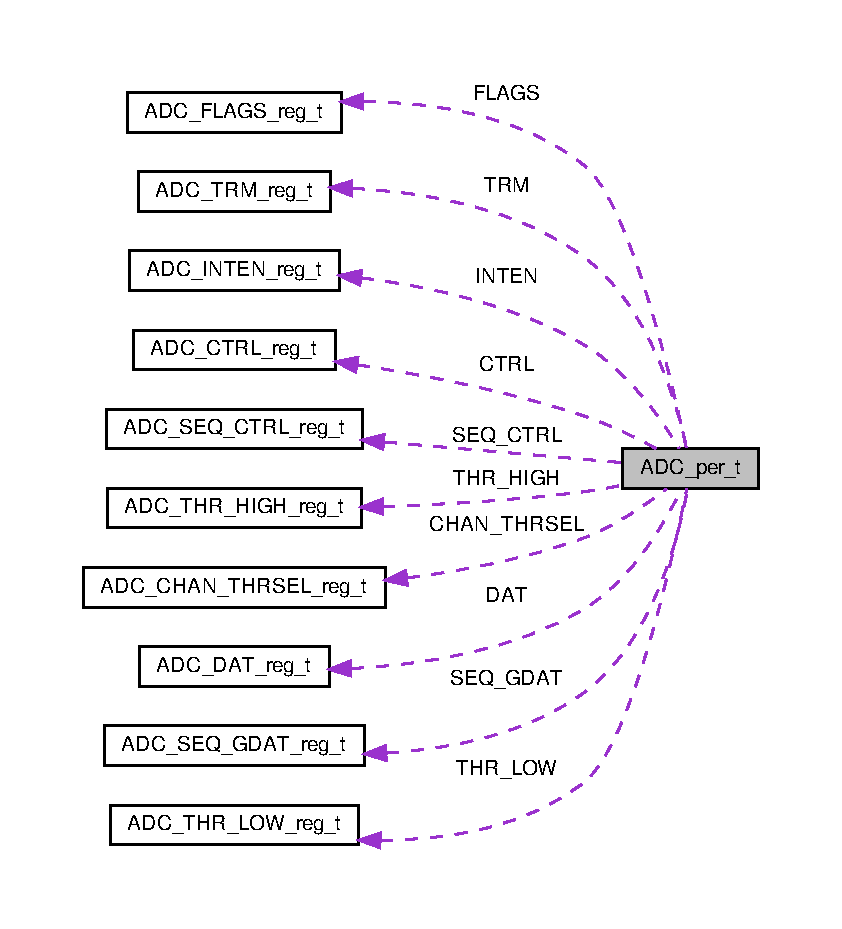
\includegraphics[width=350pt]{structADC__per__t__coll__graph}
\end{center}
\end{figure}
\begin{DoxyFields}{Campos de datos}
\mbox{\Hypertarget{HRI__ADC_8h_a127be27ae8135ea3601c6672e0677198}\label{HRI__ADC_8h_a127be27ae8135ea3601c6672e0677198}} 
\hyperlink{HRI__ADC_8h_structADC__CTRL__reg__t}{ADC\_CTRL\_reg\_t}&
CTRL&
\\
\hline

\mbox{\Hypertarget{HRI__ADC_8h_ae00d3851042af58f6b2efdc1f9c04def}\label{HRI__ADC_8h_ae00d3851042af58f6b2efdc1f9c04def}} 
const uint32\_t&
RESERVED\_1&
\\
\hline

\mbox{\Hypertarget{HRI__ADC_8h_aab65d10bc8b53b57c468cb29a1641954}\label{HRI__ADC_8h_aab65d10bc8b53b57c468cb29a1641954}} 
\hyperlink{HRI__ADC_8h_structADC__SEQ__CTRL__reg__t}{ADC\_SEQ\_CTRL\_reg\_t}&
SEQ\_CTRL\mbox{[}2\mbox{]}&
\\
\hline

\mbox{\Hypertarget{HRI__ADC_8h_adbeb451086c76cc000f9922ea939ee4b}\label{HRI__ADC_8h_adbeb451086c76cc000f9922ea939ee4b}} 
\hyperlink{HRI__ADC_8h_structADC__SEQ__GDAT__reg__t}{ADC\_SEQ\_GDAT\_reg\_t}&
SEQ\_GDAT\mbox{[}2\mbox{]}&
\\
\hline

\mbox{\Hypertarget{HRI__ADC_8h_a57a115474ec5838a5e65018d8d790ec9}\label{HRI__ADC_8h_a57a115474ec5838a5e65018d8d790ec9}} 
const uint32\_t&
RESERVED\_2\mbox{[}2\mbox{]}&
\\
\hline

\mbox{\Hypertarget{HRI__ADC_8h_a9c7e02c7b79098cd4d9cbb1ee7560519}\label{HRI__ADC_8h_a9c7e02c7b79098cd4d9cbb1ee7560519}} 
const \hyperlink{HRI__ADC_8h_structADC__DAT__reg__t}{ADC\_DAT\_reg\_t}&
DAT\mbox{[}12\mbox{]}&
\\
\hline

\mbox{\Hypertarget{HRI__ADC_8h_a122447603ba8fb72591662e6a8bdc3e9}\label{HRI__ADC_8h_a122447603ba8fb72591662e6a8bdc3e9}} 
\hyperlink{HRI__ADC_8h_structADC__THR__LOW__reg__t}{ADC\_THR\_LOW\_reg\_t}&
THR\_LOW\mbox{[}2\mbox{]}&
\\
\hline

\mbox{\Hypertarget{HRI__ADC_8h_ae7142c9897939b210404fb8a351a7c5a}\label{HRI__ADC_8h_ae7142c9897939b210404fb8a351a7c5a}} 
\hyperlink{HRI__ADC_8h_structADC__THR__HIGH__reg__t}{ADC\_THR\_HIGH\_reg\_t}&
THR\_HIGH\mbox{[}2\mbox{]}&
\\
\hline

\mbox{\Hypertarget{HRI__ADC_8h_a01b838ac35f2e109b72a5bfcba9faff6}\label{HRI__ADC_8h_a01b838ac35f2e109b72a5bfcba9faff6}} 
\hyperlink{HRI__ADC_8h_structADC__CHAN__THRSEL__reg__t}{ADC\_CHAN\_THRSEL\_reg\_t}&
CHAN\_THRSEL&
\\
\hline

\mbox{\Hypertarget{HRI__ADC_8h_a76f6ea29839c073cb62d7ea65d38c357}\label{HRI__ADC_8h_a76f6ea29839c073cb62d7ea65d38c357}} 
\hyperlink{HRI__ADC_8h_structADC__INTEN__reg__t}{ADC\_INTEN\_reg\_t}&
INTEN&
\\
\hline

\mbox{\Hypertarget{HRI__ADC_8h_a730e38f6c326544f321237af334451d0}\label{HRI__ADC_8h_a730e38f6c326544f321237af334451d0}} 
\hyperlink{HRI__ADC_8h_structADC__FLAGS__reg__t}{ADC\_FLAGS\_reg\_t}&
FLAGS&
\\
\hline

\mbox{\Hypertarget{HRI__ADC_8h_ad6658de4de5c46838c1ee63306b42749}\label{HRI__ADC_8h_ad6658de4de5c46838c1ee63306b42749}} 
\hyperlink{HRI__ADC_8h_structADC__TRM__reg__t}{ADC\_TRM\_reg\_t}&
TRM&
\\
\hline

\end{DoxyFields}

\hypertarget{HRI__CTIMER_8h}{}\section{Referencia del Archivo includes/hri/\+H\+R\+I\+\_\+\+C\+T\+I\+M\+ER.h}
\label{HRI__CTIMER_8h}\index{includes/hri/\+H\+R\+I\+\_\+\+C\+T\+I\+M\+E\+R.\+h@{includes/hri/\+H\+R\+I\+\_\+\+C\+T\+I\+M\+E\+R.\+h}}


Definiciones a nivel de registros del periferico C\+T\+I\+M\+ER (L\+P\+C845)  


{\ttfamily \#include $<$stdint.\+h$>$}\newline
Dependencia gráfica adjunta para H\+R\+I\+\_\+\+C\+T\+I\+M\+E\+R.\+h\+:\nopagebreak
\begin{figure}[H]
\begin{center}
\leavevmode
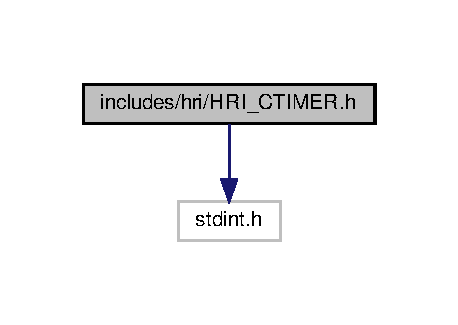
\includegraphics[width=220pt]{HRI__CTIMER_8h__incl}
\end{center}
\end{figure}
Gráfico de los archivos que directa o indirectamente incluyen a este archivo\+:\nopagebreak
\begin{figure}[H]
\begin{center}
\leavevmode
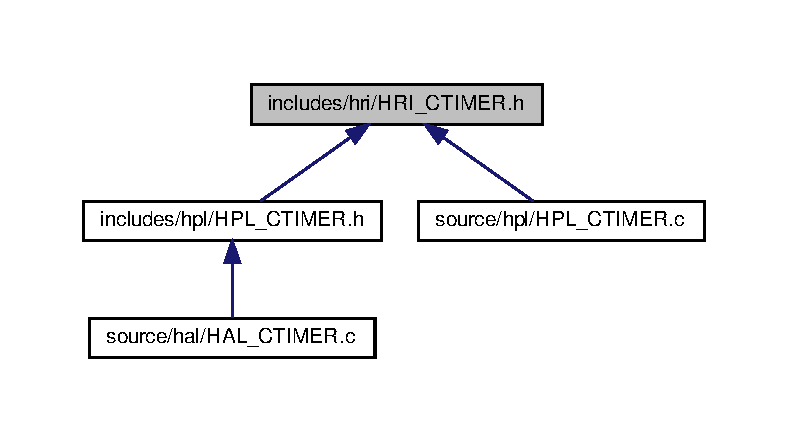
\includegraphics[width=350pt]{HRI__CTIMER_8h__dep__incl}
\end{center}
\end{figure}
\subsection*{Estructuras de datos}
\begin{DoxyCompactItemize}
\item 
struct \hyperlink{HRI__CTIMER_8h_structCTIMER__IR__reg__t}{C\+T\+I\+M\+E\+R\+\_\+\+I\+R\+\_\+reg\+\_\+t}
\item 
struct \hyperlink{HRI__CTIMER_8h_structCTIMER__TCR__reg__t}{C\+T\+I\+M\+E\+R\+\_\+\+T\+C\+R\+\_\+reg\+\_\+t}
\item 
struct \hyperlink{HRI__CTIMER_8h_structCTIMER__TC__reg__t}{C\+T\+I\+M\+E\+R\+\_\+\+T\+C\+\_\+reg\+\_\+t}
\item 
struct \hyperlink{HRI__CTIMER_8h_structCTIMER__PR__reg__t}{C\+T\+I\+M\+E\+R\+\_\+\+P\+R\+\_\+reg\+\_\+t}
\item 
struct \hyperlink{HRI__CTIMER_8h_structCTIMER__PC__reg__t}{C\+T\+I\+M\+E\+R\+\_\+\+P\+C\+\_\+reg\+\_\+t}
\item 
struct \hyperlink{HRI__CTIMER_8h_structCTIMER__MCR__reg__t}{C\+T\+I\+M\+E\+R\+\_\+\+M\+C\+R\+\_\+reg\+\_\+t}
\item 
struct \hyperlink{HRI__CTIMER_8h_structCTIMER__MR__reg__t}{C\+T\+I\+M\+E\+R\+\_\+\+M\+R\+\_\+reg\+\_\+t}
\item 
struct \hyperlink{HRI__CTIMER_8h_structCTIMER__CCR__reg__t}{C\+T\+I\+M\+E\+R\+\_\+\+C\+C\+R\+\_\+reg\+\_\+t}
\item 
struct \hyperlink{HRI__CTIMER_8h_structCTIMER__CR__reg__t}{C\+T\+I\+M\+E\+R\+\_\+\+C\+R\+\_\+reg\+\_\+t}
\item 
struct \hyperlink{HRI__CTIMER_8h_structCTIMER__EMR__reg__t}{C\+T\+I\+M\+E\+R\+\_\+\+E\+M\+R\+\_\+reg\+\_\+t}
\item 
struct \hyperlink{HRI__CTIMER_8h_structCTIMER__CTCR__reg__t}{C\+T\+I\+M\+E\+R\+\_\+\+C\+T\+C\+R\+\_\+reg\+\_\+t}
\item 
struct \hyperlink{HRI__CTIMER_8h_structCTIMER__PWMC__reg__t}{C\+T\+I\+M\+E\+R\+\_\+\+P\+W\+M\+C\+\_\+reg\+\_\+t}
\item 
struct \hyperlink{HRI__CTIMER_8h_structCTIMER__MSR__reg__t}{C\+T\+I\+M\+E\+R\+\_\+\+M\+S\+R\+\_\+reg\+\_\+t}
\item 
struct \hyperlink{HRI__CTIMER_8h_structCTIMER__per__t}{C\+T\+I\+M\+E\+R\+\_\+per\+\_\+t}
\end{DoxyCompactItemize}
\subsection*{defines}
\begin{DoxyCompactItemize}
\item 
\mbox{\Hypertarget{HRI__CTIMER_8h_a53d6600a02b206837769c0e2b7be322a}\label{HRI__CTIMER_8h_a53d6600a02b206837769c0e2b7be322a}} 
\#define {\bfseries C\+T\+I\+M\+E\+R\+\_\+\+B\+A\+SE}~0x40038000
\end{DoxyCompactItemize}


\subsection{Descripción detallada}
Definiciones a nivel de registros del periferico C\+T\+I\+M\+ER (L\+P\+C845) 

\begin{DoxyAuthor}{Autor}
Augusto Santini 
\end{DoxyAuthor}
\begin{DoxyDate}{Fecha}
3/2020 
\end{DoxyDate}
\begin{DoxyVersion}{Versión}
1.\+0 
\end{DoxyVersion}


\subsection{Documentación de las estructuras de datos}
\index{C\+T\+I\+M\+E\+R\+\_\+\+I\+R\+\_\+reg\+\_\+t@{C\+T\+I\+M\+E\+R\+\_\+\+I\+R\+\_\+reg\+\_\+t}}\label{structCTIMER__IR__reg__t}
\Hypertarget{HRI__CTIMER_8h_structCTIMER__IR__reg__t}
\subsubsection{struct C\+T\+I\+M\+E\+R\+\_\+\+I\+R\+\_\+reg\+\_\+t}
\begin{DoxyFields}{Campos de datos}
\mbox{\Hypertarget{HRI__CTIMER_8h_a21ada62f36e0bdd9190f43c0e6626abb}\label{HRI__CTIMER_8h_a21ada62f36e0bdd9190f43c0e6626abb}} 
uint32\_t&
MR0INT: 1&
\\
\hline

\mbox{\Hypertarget{HRI__CTIMER_8h_a7401c1487342aee2e84e90ee7eb37cf9}\label{HRI__CTIMER_8h_a7401c1487342aee2e84e90ee7eb37cf9}} 
uint32\_t&
MR1INT: 1&
\\
\hline

\mbox{\Hypertarget{HRI__CTIMER_8h_a1039f8d61d5c24fb0a4beaf031c481ee}\label{HRI__CTIMER_8h_a1039f8d61d5c24fb0a4beaf031c481ee}} 
uint32\_t&
MR2INT: 1&
\\
\hline

\mbox{\Hypertarget{HRI__CTIMER_8h_a8a2f7e54904914ef2d8adbe75ca92552}\label{HRI__CTIMER_8h_a8a2f7e54904914ef2d8adbe75ca92552}} 
uint32\_t&
MR3INT: 1&
\\
\hline

\mbox{\Hypertarget{HRI__CTIMER_8h_a14e6f8809c2c69273cee2e67c1301e2b}\label{HRI__CTIMER_8h_a14e6f8809c2c69273cee2e67c1301e2b}} 
uint32\_t&
CR0INT: 1&
\\
\hline

\mbox{\Hypertarget{HRI__CTIMER_8h_a55220f82473994fc55f40afa622d63da}\label{HRI__CTIMER_8h_a55220f82473994fc55f40afa622d63da}} 
uint32\_t&
CR1INT: 1&
\\
\hline

\mbox{\Hypertarget{HRI__CTIMER_8h_adf9483d0b582b8d8513d2d877cad54bf}\label{HRI__CTIMER_8h_adf9483d0b582b8d8513d2d877cad54bf}} 
uint32\_t&
CR2INT: 1&
\\
\hline

\mbox{\Hypertarget{HRI__CTIMER_8h_a73a78629b5d8c8fc84fba714932716c7}\label{HRI__CTIMER_8h_a73a78629b5d8c8fc84fba714932716c7}} 
uint32\_t&
CR3INT: 1&
\\
\hline

\mbox{\Hypertarget{HRI__CTIMER_8h_a49ec0668bb6377952c2234d9bea70118}\label{HRI__CTIMER_8h_a49ec0668bb6377952c2234d9bea70118}} 
uint32\_t&
\_\_pad0\_\_: 24&
\\
\hline

\end{DoxyFields}
\index{C\+T\+I\+M\+E\+R\+\_\+\+T\+C\+R\+\_\+reg\+\_\+t@{C\+T\+I\+M\+E\+R\+\_\+\+T\+C\+R\+\_\+reg\+\_\+t}}\label{structCTIMER__TCR__reg__t}
\Hypertarget{HRI__CTIMER_8h_structCTIMER__TCR__reg__t}
\subsubsection{struct C\+T\+I\+M\+E\+R\+\_\+\+T\+C\+R\+\_\+reg\+\_\+t}
\begin{DoxyFields}{Campos de datos}
\mbox{\Hypertarget{HRI__CTIMER_8h_aba1a0f607efaebcf49c737418073a614}\label{HRI__CTIMER_8h_aba1a0f607efaebcf49c737418073a614}} 
uint32\_t&
CEN: 1&
\\
\hline

\mbox{\Hypertarget{HRI__CTIMER_8h_a9cf8f9831b7ed2181e02546a8436c70d}\label{HRI__CTIMER_8h_a9cf8f9831b7ed2181e02546a8436c70d}} 
uint32\_t&
CRST: 1&
\\
\hline

\mbox{\Hypertarget{HRI__CTIMER_8h_a10c1cf4c599a2f31e5217ee72f0ad59e}\label{HRI__CTIMER_8h_a10c1cf4c599a2f31e5217ee72f0ad59e}} 
uint32\_t&
\_\_pad0\_\_: 30&
\\
\hline

\end{DoxyFields}
\index{C\+T\+I\+M\+E\+R\+\_\+\+T\+C\+\_\+reg\+\_\+t@{C\+T\+I\+M\+E\+R\+\_\+\+T\+C\+\_\+reg\+\_\+t}}\label{structCTIMER__TC__reg__t}
\Hypertarget{HRI__CTIMER_8h_structCTIMER__TC__reg__t}
\subsubsection{struct C\+T\+I\+M\+E\+R\+\_\+\+T\+C\+\_\+reg\+\_\+t}
\begin{DoxyFields}{Campos de datos}
\mbox{\Hypertarget{HRI__CTIMER_8h_a42d27d8a319ac35284bc75d15e97fcd1}\label{HRI__CTIMER_8h_a42d27d8a319ac35284bc75d15e97fcd1}} 
uint32\_t&
TCVAL&
\\
\hline

\end{DoxyFields}
\index{C\+T\+I\+M\+E\+R\+\_\+\+P\+R\+\_\+reg\+\_\+t@{C\+T\+I\+M\+E\+R\+\_\+\+P\+R\+\_\+reg\+\_\+t}}\label{structCTIMER__PR__reg__t}
\Hypertarget{HRI__CTIMER_8h_structCTIMER__PR__reg__t}
\subsubsection{struct C\+T\+I\+M\+E\+R\+\_\+\+P\+R\+\_\+reg\+\_\+t}
\begin{DoxyFields}{Campos de datos}
\mbox{\Hypertarget{HRI__CTIMER_8h_ad2feab046593bd76035cacdcc7a97701}\label{HRI__CTIMER_8h_ad2feab046593bd76035cacdcc7a97701}} 
uint32\_t&
PRVAL&
\\
\hline

\end{DoxyFields}
\index{C\+T\+I\+M\+E\+R\+\_\+\+P\+C\+\_\+reg\+\_\+t@{C\+T\+I\+M\+E\+R\+\_\+\+P\+C\+\_\+reg\+\_\+t}}\label{structCTIMER__PC__reg__t}
\Hypertarget{HRI__CTIMER_8h_structCTIMER__PC__reg__t}
\subsubsection{struct C\+T\+I\+M\+E\+R\+\_\+\+P\+C\+\_\+reg\+\_\+t}
\begin{DoxyFields}{Campos de datos}
\mbox{\Hypertarget{HRI__CTIMER_8h_aa0bce50cf548360786dd7e8660725ce6}\label{HRI__CTIMER_8h_aa0bce50cf548360786dd7e8660725ce6}} 
uint32\_t&
PCVAL&
\\
\hline

\end{DoxyFields}
\index{C\+T\+I\+M\+E\+R\+\_\+\+M\+C\+R\+\_\+reg\+\_\+t@{C\+T\+I\+M\+E\+R\+\_\+\+M\+C\+R\+\_\+reg\+\_\+t}}\label{structCTIMER__MCR__reg__t}
\Hypertarget{HRI__CTIMER_8h_structCTIMER__MCR__reg__t}
\subsubsection{struct C\+T\+I\+M\+E\+R\+\_\+\+M\+C\+R\+\_\+reg\+\_\+t}
\begin{DoxyFields}{Campos de datos}
\mbox{\Hypertarget{HRI__CTIMER_8h_a036daec530a0900bb47dc57e0763fe3c}\label{HRI__CTIMER_8h_a036daec530a0900bb47dc57e0763fe3c}} 
uint32\_t&
MR0I: 1&
\\
\hline

\mbox{\Hypertarget{HRI__CTIMER_8h_a152df8751d98b0930e75845560df9aed}\label{HRI__CTIMER_8h_a152df8751d98b0930e75845560df9aed}} 
uint32\_t&
MR0R: 1&
\\
\hline

\mbox{\Hypertarget{HRI__CTIMER_8h_aa84ed7bca6beb2c91219df9caad31065}\label{HRI__CTIMER_8h_aa84ed7bca6beb2c91219df9caad31065}} 
uint32\_t&
MR0S: 1&
\\
\hline

\mbox{\Hypertarget{HRI__CTIMER_8h_af937510bdc4775f521e4d6a2546c3aec}\label{HRI__CTIMER_8h_af937510bdc4775f521e4d6a2546c3aec}} 
uint32\_t&
MR1I: 1&
\\
\hline

\mbox{\Hypertarget{HRI__CTIMER_8h_a2d0d7a1ace098a6facf87460322a4f5b}\label{HRI__CTIMER_8h_a2d0d7a1ace098a6facf87460322a4f5b}} 
uint32\_t&
MR1R: 1&
\\
\hline

\mbox{\Hypertarget{HRI__CTIMER_8h_a0eef54633f64b0e5b83788472b9b2766}\label{HRI__CTIMER_8h_a0eef54633f64b0e5b83788472b9b2766}} 
uint32\_t&
MR1S: 1&
\\
\hline

\mbox{\Hypertarget{HRI__CTIMER_8h_a09291cb9060a0dbce3d6468761926419}\label{HRI__CTIMER_8h_a09291cb9060a0dbce3d6468761926419}} 
uint32\_t&
MR2I: 1&
\\
\hline

\mbox{\Hypertarget{HRI__CTIMER_8h_af613ef8edafae9db552e85af518d013e}\label{HRI__CTIMER_8h_af613ef8edafae9db552e85af518d013e}} 
uint32\_t&
MR2R: 1&
\\
\hline

\mbox{\Hypertarget{HRI__CTIMER_8h_af735d35dc0046793a54de96b65c3d611}\label{HRI__CTIMER_8h_af735d35dc0046793a54de96b65c3d611}} 
uint32\_t&
MR2S: 1&
\\
\hline

\mbox{\Hypertarget{HRI__CTIMER_8h_abe2f9fceac9fa6afa789ab089d9b86cc}\label{HRI__CTIMER_8h_abe2f9fceac9fa6afa789ab089d9b86cc}} 
uint32\_t&
MR3I: 1&
\\
\hline

\mbox{\Hypertarget{HRI__CTIMER_8h_a2b06907733d402f4f007e437aaf5c65b}\label{HRI__CTIMER_8h_a2b06907733d402f4f007e437aaf5c65b}} 
uint32\_t&
MR3R: 1&
\\
\hline

\mbox{\Hypertarget{HRI__CTIMER_8h_a99b3d24b53b24fa34cacb5bb93962274}\label{HRI__CTIMER_8h_a99b3d24b53b24fa34cacb5bb93962274}} 
uint32\_t&
MR3S: 1&
\\
\hline

\mbox{\Hypertarget{HRI__CTIMER_8h_a411dc61b72dd1fecbcdb49a5fef70a3c}\label{HRI__CTIMER_8h_a411dc61b72dd1fecbcdb49a5fef70a3c}} 
uint32\_t&
\_\_pad0\_\_: 12&
\\
\hline

\mbox{\Hypertarget{HRI__CTIMER_8h_aa65e5219edc0becce0af121e86c38d48}\label{HRI__CTIMER_8h_aa65e5219edc0becce0af121e86c38d48}} 
uint32\_t&
MR0RL: 1&
\\
\hline

\mbox{\Hypertarget{HRI__CTIMER_8h_a35a9c552d8f460cbad12c31c4aa90501}\label{HRI__CTIMER_8h_a35a9c552d8f460cbad12c31c4aa90501}} 
uint32\_t&
MR1RL: 1&
\\
\hline

\mbox{\Hypertarget{HRI__CTIMER_8h_a0fb8f6e16d00101606202cce990f899b}\label{HRI__CTIMER_8h_a0fb8f6e16d00101606202cce990f899b}} 
uint32\_t&
MR2RL: 1&
\\
\hline

\mbox{\Hypertarget{HRI__CTIMER_8h_adbb7c0a52a2d713d1de1a3e12377ca70}\label{HRI__CTIMER_8h_adbb7c0a52a2d713d1de1a3e12377ca70}} 
uint32\_t&
MR3RL: 1&
\\
\hline

\mbox{\Hypertarget{HRI__CTIMER_8h_a9ed94a0fc421d053dc4f236aa55f2f6e}\label{HRI__CTIMER_8h_a9ed94a0fc421d053dc4f236aa55f2f6e}} 
uint32\_t&
\_\_pad1\_\_: 4&
\\
\hline

\end{DoxyFields}
\index{C\+T\+I\+M\+E\+R\+\_\+\+M\+R\+\_\+reg\+\_\+t@{C\+T\+I\+M\+E\+R\+\_\+\+M\+R\+\_\+reg\+\_\+t}}\label{structCTIMER__MR__reg__t}
\Hypertarget{HRI__CTIMER_8h_structCTIMER__MR__reg__t}
\subsubsection{struct C\+T\+I\+M\+E\+R\+\_\+\+M\+R\+\_\+reg\+\_\+t}
\begin{DoxyFields}{Campos de datos}
\mbox{\Hypertarget{HRI__CTIMER_8h_aa93b448eae5ff3a11c88a03d8c7c5c85}\label{HRI__CTIMER_8h_aa93b448eae5ff3a11c88a03d8c7c5c85}} 
uint32\_t&
MATCH&
\\
\hline

\end{DoxyFields}
\index{C\+T\+I\+M\+E\+R\+\_\+\+C\+C\+R\+\_\+reg\+\_\+t@{C\+T\+I\+M\+E\+R\+\_\+\+C\+C\+R\+\_\+reg\+\_\+t}}\label{structCTIMER__CCR__reg__t}
\Hypertarget{HRI__CTIMER_8h_structCTIMER__CCR__reg__t}
\subsubsection{struct C\+T\+I\+M\+E\+R\+\_\+\+C\+C\+R\+\_\+reg\+\_\+t}
\begin{DoxyFields}{Campos de datos}
\mbox{\Hypertarget{HRI__CTIMER_8h_ae0e9e94846dc516a3bc5f8c5a6e10d78}\label{HRI__CTIMER_8h_ae0e9e94846dc516a3bc5f8c5a6e10d78}} 
uint32\_t&
CAP0RE: 1&
\\
\hline

\mbox{\Hypertarget{HRI__CTIMER_8h_a0b16448179ee330bb6123af9bb27d137}\label{HRI__CTIMER_8h_a0b16448179ee330bb6123af9bb27d137}} 
uint32\_t&
CAP0FE: 1&
\\
\hline

\mbox{\Hypertarget{HRI__CTIMER_8h_a00220989c6dd9b7c23f8b145a2a30a2d}\label{HRI__CTIMER_8h_a00220989c6dd9b7c23f8b145a2a30a2d}} 
uint32\_t&
CAP0I: 1&
\\
\hline

\mbox{\Hypertarget{HRI__CTIMER_8h_a01a57c8c75795b18565defca5aeb35a3}\label{HRI__CTIMER_8h_a01a57c8c75795b18565defca5aeb35a3}} 
uint32\_t&
CAP1RE: 1&
\\
\hline

\mbox{\Hypertarget{HRI__CTIMER_8h_a19c49d638cb1b18639a1cd5776d499ec}\label{HRI__CTIMER_8h_a19c49d638cb1b18639a1cd5776d499ec}} 
uint32\_t&
CAP1FE: 1&
\\
\hline

\mbox{\Hypertarget{HRI__CTIMER_8h_a467f010c5eb7bbbbae95f15a9d289fc1}\label{HRI__CTIMER_8h_a467f010c5eb7bbbbae95f15a9d289fc1}} 
uint32\_t&
CAP1I: 1&
\\
\hline

\mbox{\Hypertarget{HRI__CTIMER_8h_aedc72fac494dc0ba132a9b0f74f0e112}\label{HRI__CTIMER_8h_aedc72fac494dc0ba132a9b0f74f0e112}} 
uint32\_t&
CAP2RE: 1&
\\
\hline

\mbox{\Hypertarget{HRI__CTIMER_8h_aded9b598dba74aaa8376eaeea0c77e4b}\label{HRI__CTIMER_8h_aded9b598dba74aaa8376eaeea0c77e4b}} 
uint32\_t&
CAP2FE: 1&
\\
\hline

\mbox{\Hypertarget{HRI__CTIMER_8h_abd549b4f5f81d91a5a25c0737a7fc387}\label{HRI__CTIMER_8h_abd549b4f5f81d91a5a25c0737a7fc387}} 
uint32\_t&
CAP2I: 1&
\\
\hline

\mbox{\Hypertarget{HRI__CTIMER_8h_aee73cd37d16b42568bf74c2245cf78cb}\label{HRI__CTIMER_8h_aee73cd37d16b42568bf74c2245cf78cb}} 
uint32\_t&
CAP3RE: 1&
\\
\hline

\mbox{\Hypertarget{HRI__CTIMER_8h_a9fd0c9f99d5e9ec7258ea9993f1c3d59}\label{HRI__CTIMER_8h_a9fd0c9f99d5e9ec7258ea9993f1c3d59}} 
uint32\_t&
CAP3FE: 1&
\\
\hline

\mbox{\Hypertarget{HRI__CTIMER_8h_ae23a168761d4fd9877ae962efc453b36}\label{HRI__CTIMER_8h_ae23a168761d4fd9877ae962efc453b36}} 
uint32\_t&
CAP3I: 1&
\\
\hline

\mbox{\Hypertarget{HRI__CTIMER_8h_af0b6e24e9a450512ea8ddcadbaec7c4d}\label{HRI__CTIMER_8h_af0b6e24e9a450512ea8ddcadbaec7c4d}} 
uint32\_t&
\_\_pad0\_\_: 20&
\\
\hline

\end{DoxyFields}
\index{C\+T\+I\+M\+E\+R\+\_\+\+C\+R\+\_\+reg\+\_\+t@{C\+T\+I\+M\+E\+R\+\_\+\+C\+R\+\_\+reg\+\_\+t}}\label{structCTIMER__CR__reg__t}
\Hypertarget{HRI__CTIMER_8h_structCTIMER__CR__reg__t}
\subsubsection{struct C\+T\+I\+M\+E\+R\+\_\+\+C\+R\+\_\+reg\+\_\+t}
\begin{DoxyFields}{Campos de datos}
\mbox{\Hypertarget{HRI__CTIMER_8h_adf858f7c70c97898a398932cdd11b41e}\label{HRI__CTIMER_8h_adf858f7c70c97898a398932cdd11b41e}} 
uint32\_t&
CAP&
\\
\hline

\end{DoxyFields}
\index{C\+T\+I\+M\+E\+R\+\_\+\+E\+M\+R\+\_\+reg\+\_\+t@{C\+T\+I\+M\+E\+R\+\_\+\+E\+M\+R\+\_\+reg\+\_\+t}}\label{structCTIMER__EMR__reg__t}
\Hypertarget{HRI__CTIMER_8h_structCTIMER__EMR__reg__t}
\subsubsection{struct C\+T\+I\+M\+E\+R\+\_\+\+E\+M\+R\+\_\+reg\+\_\+t}
\begin{DoxyFields}{Campos de datos}
\mbox{\Hypertarget{HRI__CTIMER_8h_a8d92cb0f0eeb39be4c4101e76f459c16}\label{HRI__CTIMER_8h_a8d92cb0f0eeb39be4c4101e76f459c16}} 
uint32\_t&
EM0: 1&
\\
\hline

\mbox{\Hypertarget{HRI__CTIMER_8h_acaa7af7bf15764423bb7accbbe7fb299}\label{HRI__CTIMER_8h_acaa7af7bf15764423bb7accbbe7fb299}} 
uint32\_t&
EM1: 1&
\\
\hline

\mbox{\Hypertarget{HRI__CTIMER_8h_a63c539264825d005abd4d16ebb059489}\label{HRI__CTIMER_8h_a63c539264825d005abd4d16ebb059489}} 
uint32\_t&
EM2: 1&
\\
\hline

\mbox{\Hypertarget{HRI__CTIMER_8h_a4a91c7a1b54919c95403c2180f507bf8}\label{HRI__CTIMER_8h_a4a91c7a1b54919c95403c2180f507bf8}} 
uint32\_t&
EM3: 1&
\\
\hline

\mbox{\Hypertarget{HRI__CTIMER_8h_a9cffc149036fa2f68ae6e4b5617f6545}\label{HRI__CTIMER_8h_a9cffc149036fa2f68ae6e4b5617f6545}} 
uint32\_t&
EMC0: 2&
\\
\hline

\mbox{\Hypertarget{HRI__CTIMER_8h_a388a233a66276a69bfba39e6b8c8ea8b}\label{HRI__CTIMER_8h_a388a233a66276a69bfba39e6b8c8ea8b}} 
uint32\_t&
EMC1: 2&
\\
\hline

\mbox{\Hypertarget{HRI__CTIMER_8h_a461052392f031d61bd1d2cc6a37cf378}\label{HRI__CTIMER_8h_a461052392f031d61bd1d2cc6a37cf378}} 
uint32\_t&
EMC2: 2&
\\
\hline

\mbox{\Hypertarget{HRI__CTIMER_8h_abae87ed1c2513a370e36a2f6cb95a724}\label{HRI__CTIMER_8h_abae87ed1c2513a370e36a2f6cb95a724}} 
uint32\_t&
EMC3: 2&
\\
\hline

\mbox{\Hypertarget{HRI__CTIMER_8h_a1c826498e8b6d151fa6bf1aca3f4c75b}\label{HRI__CTIMER_8h_a1c826498e8b6d151fa6bf1aca3f4c75b}} 
uint32\_t&
\_\_pad0\_\_: 20&
\\
\hline

\end{DoxyFields}
\index{C\+T\+I\+M\+E\+R\+\_\+\+C\+T\+C\+R\+\_\+reg\+\_\+t@{C\+T\+I\+M\+E\+R\+\_\+\+C\+T\+C\+R\+\_\+reg\+\_\+t}}\label{structCTIMER__CTCR__reg__t}
\Hypertarget{HRI__CTIMER_8h_structCTIMER__CTCR__reg__t}
\subsubsection{struct C\+T\+I\+M\+E\+R\+\_\+\+C\+T\+C\+R\+\_\+reg\+\_\+t}
\begin{DoxyFields}{Campos de datos}
\mbox{\Hypertarget{HRI__CTIMER_8h_adf68f3c574336366d46ff2e6988bdf5c}\label{HRI__CTIMER_8h_adf68f3c574336366d46ff2e6988bdf5c}} 
uint32\_t&
CTMODE: 2&
\\
\hline

\mbox{\Hypertarget{HRI__CTIMER_8h_a87ada47ba825b61cd209f01d1a38f3ca}\label{HRI__CTIMER_8h_a87ada47ba825b61cd209f01d1a38f3ca}} 
uint32\_t&
CINSEL: 2&
\\
\hline

\mbox{\Hypertarget{HRI__CTIMER_8h_a515114a5edae51c27ba317ccb64661d4}\label{HRI__CTIMER_8h_a515114a5edae51c27ba317ccb64661d4}} 
uint32\_t&
ENCC: 1&
\\
\hline

\mbox{\Hypertarget{HRI__CTIMER_8h_a750ba6640a5e28a43783127a5c5dca51}\label{HRI__CTIMER_8h_a750ba6640a5e28a43783127a5c5dca51}} 
uint32\_t&
SELCC: 3&
\\
\hline

\mbox{\Hypertarget{HRI__CTIMER_8h_ac374e0a5b722e2599580f91491b20f0d}\label{HRI__CTIMER_8h_ac374e0a5b722e2599580f91491b20f0d}} 
uint32\_t&
\_\_pad0\_\_: 24&
\\
\hline

\end{DoxyFields}
\index{C\+T\+I\+M\+E\+R\+\_\+\+P\+W\+M\+C\+\_\+reg\+\_\+t@{C\+T\+I\+M\+E\+R\+\_\+\+P\+W\+M\+C\+\_\+reg\+\_\+t}}\label{structCTIMER__PWMC__reg__t}
\Hypertarget{HRI__CTIMER_8h_structCTIMER__PWMC__reg__t}
\subsubsection{struct C\+T\+I\+M\+E\+R\+\_\+\+P\+W\+M\+C\+\_\+reg\+\_\+t}
\begin{DoxyFields}{Campos de datos}
\mbox{\Hypertarget{HRI__CTIMER_8h_a31066f20289e1433fc702819c6ad2beb}\label{HRI__CTIMER_8h_a31066f20289e1433fc702819c6ad2beb}} 
uint32\_t&
PWMEN0: 1&
\\
\hline

\mbox{\Hypertarget{HRI__CTIMER_8h_a36151d94c6ddd473c38b49ac2b2635c0}\label{HRI__CTIMER_8h_a36151d94c6ddd473c38b49ac2b2635c0}} 
uint32\_t&
PWMEN1: 1&
\\
\hline

\mbox{\Hypertarget{HRI__CTIMER_8h_a56029247361d112c5b208c60c059bfa2}\label{HRI__CTIMER_8h_a56029247361d112c5b208c60c059bfa2}} 
uint32\_t&
PWMEN2: 1&
\\
\hline

\mbox{\Hypertarget{HRI__CTIMER_8h_a3331a8e4a519e1f9843c250285c01573}\label{HRI__CTIMER_8h_a3331a8e4a519e1f9843c250285c01573}} 
uint32\_t&
PWMEN3: 1&
\\
\hline

\mbox{\Hypertarget{HRI__CTIMER_8h_aa83ecd8f1bf3018813dca516dddbd070}\label{HRI__CTIMER_8h_aa83ecd8f1bf3018813dca516dddbd070}} 
uint32\_t&
\_\_pad0\_\_: 28&
\\
\hline

\end{DoxyFields}
\index{C\+T\+I\+M\+E\+R\+\_\+\+M\+S\+R\+\_\+reg\+\_\+t@{C\+T\+I\+M\+E\+R\+\_\+\+M\+S\+R\+\_\+reg\+\_\+t}}\label{structCTIMER__MSR__reg__t}
\Hypertarget{HRI__CTIMER_8h_structCTIMER__MSR__reg__t}
\subsubsection{struct C\+T\+I\+M\+E\+R\+\_\+\+M\+S\+R\+\_\+reg\+\_\+t}
\begin{DoxyFields}{Campos de datos}
\mbox{\Hypertarget{HRI__CTIMER_8h_a50664c656395614ca569996176a7646c}\label{HRI__CTIMER_8h_a50664c656395614ca569996176a7646c}} 
uint32\_t&
SHADOW&
\\
\hline

\end{DoxyFields}
\index{C\+T\+I\+M\+E\+R\+\_\+per\+\_\+t@{C\+T\+I\+M\+E\+R\+\_\+per\+\_\+t}}\label{structCTIMER__per__t}
\Hypertarget{HRI__CTIMER_8h_structCTIMER__per__t}
\subsubsection{struct C\+T\+I\+M\+E\+R\+\_\+per\+\_\+t}


Diagrama de colaboración para C\+T\+I\+M\+E\+R\+\_\+per\+\_\+t\+:\nopagebreak
\begin{figure}[H]
\begin{center}
\leavevmode
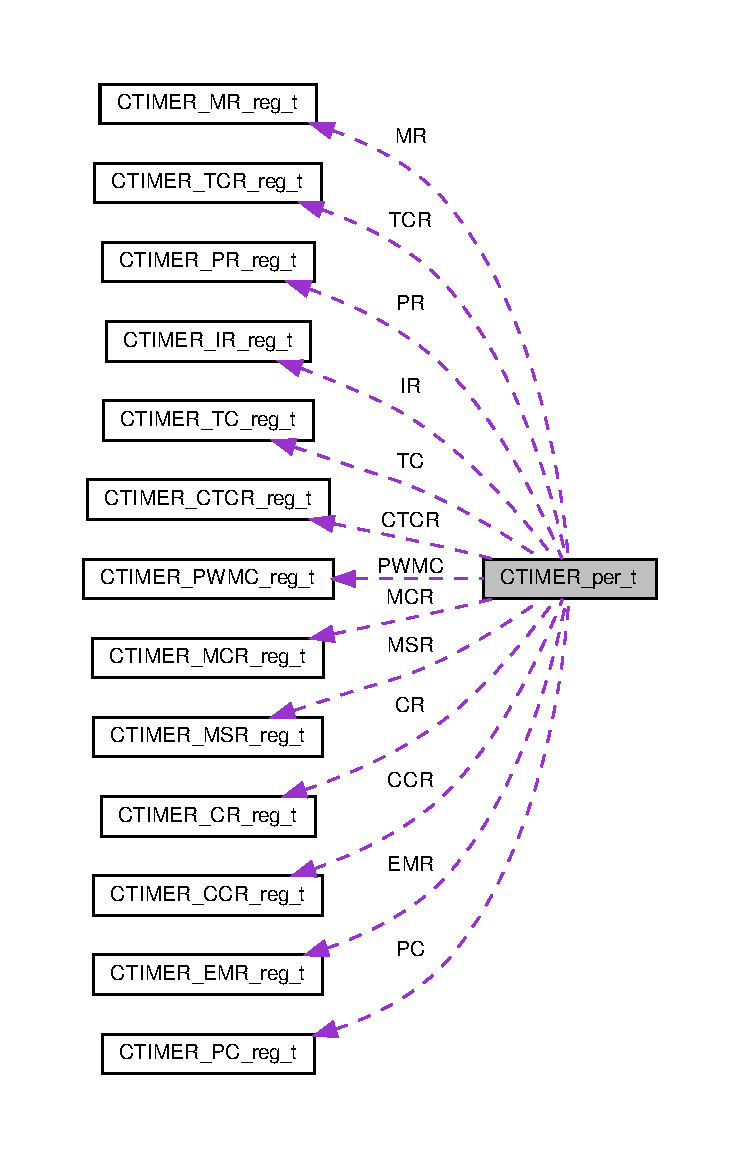
\includegraphics[width=350pt]{structCTIMER__per__t__coll__graph}
\end{center}
\end{figure}
\begin{DoxyFields}{Campos de datos}
\mbox{\Hypertarget{HRI__CTIMER_8h_ae64bb402dbdf3f530f467cfe3182e1fd}\label{HRI__CTIMER_8h_ae64bb402dbdf3f530f467cfe3182e1fd}} 
\hyperlink{HRI__CTIMER_8h_structCTIMER__IR__reg__t}{CTIMER\_IR\_reg\_t}&
IR&
\\
\hline

\mbox{\Hypertarget{HRI__CTIMER_8h_a951ce6cfd1a1f5d644b653b15ab90e03}\label{HRI__CTIMER_8h_a951ce6cfd1a1f5d644b653b15ab90e03}} 
\hyperlink{HRI__CTIMER_8h_structCTIMER__TCR__reg__t}{CTIMER\_TCR\_reg\_t}&
TCR&
\\
\hline

\mbox{\Hypertarget{HRI__CTIMER_8h_aadd1c3e651cf7603f855707cdc7b9f25}\label{HRI__CTIMER_8h_aadd1c3e651cf7603f855707cdc7b9f25}} 
\hyperlink{HRI__CTIMER_8h_structCTIMER__TC__reg__t}{CTIMER\_TC\_reg\_t}&
TC&
\\
\hline

\mbox{\Hypertarget{HRI__CTIMER_8h_a7e266826c4a5ca185ad44d414ebb24ac}\label{HRI__CTIMER_8h_a7e266826c4a5ca185ad44d414ebb24ac}} 
\hyperlink{HRI__CTIMER_8h_structCTIMER__PR__reg__t}{CTIMER\_PR\_reg\_t}&
PR&
\\
\hline

\mbox{\Hypertarget{HRI__CTIMER_8h_aa03d3af9f3b2320cb60b0221f23c6065}\label{HRI__CTIMER_8h_aa03d3af9f3b2320cb60b0221f23c6065}} 
\hyperlink{HRI__CTIMER_8h_structCTIMER__PC__reg__t}{CTIMER\_PC\_reg\_t}&
PC&
\\
\hline

\mbox{\Hypertarget{HRI__CTIMER_8h_a443de577bc88be25ea7925ab8f41822d}\label{HRI__CTIMER_8h_a443de577bc88be25ea7925ab8f41822d}} 
\hyperlink{HRI__CTIMER_8h_structCTIMER__MCR__reg__t}{CTIMER\_MCR\_reg\_t}&
MCR&
\\
\hline

\mbox{\Hypertarget{HRI__CTIMER_8h_ac004182b0f2da3f9bc9d0813d1eb65d6}\label{HRI__CTIMER_8h_ac004182b0f2da3f9bc9d0813d1eb65d6}} 
\hyperlink{HRI__CTIMER_8h_structCTIMER__MR__reg__t}{CTIMER\_MR\_reg\_t}&
MR\mbox{[}4\mbox{]}&
\\
\hline

\mbox{\Hypertarget{HRI__CTIMER_8h_ac63a93a17374289bc020f9de82156ca0}\label{HRI__CTIMER_8h_ac63a93a17374289bc020f9de82156ca0}} 
\hyperlink{HRI__CTIMER_8h_structCTIMER__CCR__reg__t}{CTIMER\_CCR\_reg\_t}&
CCR&
\\
\hline

\mbox{\Hypertarget{HRI__CTIMER_8h_af83165f0a6dce88eb4e6294de8a6962a}\label{HRI__CTIMER_8h_af83165f0a6dce88eb4e6294de8a6962a}} 
const \hyperlink{HRI__CTIMER_8h_structCTIMER__CR__reg__t}{CTIMER\_CR\_reg\_t}&
CR\mbox{[}4\mbox{]}&
\\
\hline

\mbox{\Hypertarget{HRI__CTIMER_8h_a69e560ccd4646847ed005b283ccb6a64}\label{HRI__CTIMER_8h_a69e560ccd4646847ed005b283ccb6a64}} 
\hyperlink{HRI__CTIMER_8h_structCTIMER__EMR__reg__t}{CTIMER\_EMR\_reg\_t}&
EMR&
\\
\hline

\mbox{\Hypertarget{HRI__CTIMER_8h_a7dee79d688bb52dda81b8aebd765869d}\label{HRI__CTIMER_8h_a7dee79d688bb52dda81b8aebd765869d}} 
const uint32\_t&
RESERVED\mbox{[}12\mbox{]}&
\\
\hline

\mbox{\Hypertarget{HRI__CTIMER_8h_a0c288844f7c6a04f3e71b57320c2775a}\label{HRI__CTIMER_8h_a0c288844f7c6a04f3e71b57320c2775a}} 
\hyperlink{HRI__CTIMER_8h_structCTIMER__CTCR__reg__t}{CTIMER\_CTCR\_reg\_t}&
CTCR&
\\
\hline

\mbox{\Hypertarget{HRI__CTIMER_8h_a49a2636edcbffd1f6a5de59255a03941}\label{HRI__CTIMER_8h_a49a2636edcbffd1f6a5de59255a03941}} 
\hyperlink{HRI__CTIMER_8h_structCTIMER__PWMC__reg__t}{CTIMER\_PWMC\_reg\_t}&
PWMC&
\\
\hline

\mbox{\Hypertarget{HRI__CTIMER_8h_a538a7c42ccabd7e69893be06187a9334}\label{HRI__CTIMER_8h_a538a7c42ccabd7e69893be06187a9334}} 
\hyperlink{HRI__CTIMER_8h_structCTIMER__MSR__reg__t}{CTIMER\_MSR\_reg\_t}&
MSR\mbox{[}4\mbox{]}&
\\
\hline

\end{DoxyFields}

\hypertarget{HRI__DAC_8h}{}\section{Referencia del Archivo includes/hri/\+H\+R\+I\+\_\+\+D\+AC.h}
\label{HRI__DAC_8h}\index{includes/hri/\+H\+R\+I\+\_\+\+D\+A\+C.\+h@{includes/hri/\+H\+R\+I\+\_\+\+D\+A\+C.\+h}}


Declaraciones a nivel de registros del D\+AC (L\+P\+C845)  


{\ttfamily \#include $<$stdint.\+h$>$}\newline
Dependencia gráfica adjunta para H\+R\+I\+\_\+\+D\+A\+C.\+h\+:\nopagebreak
\begin{figure}[H]
\begin{center}
\leavevmode
\includegraphics[width=202pt]{da/d09/HRI__DAC_8h__incl}
\end{center}
\end{figure}
Gráfico de los archivos que directa o indirectamente incluyen a este archivo\+:\nopagebreak
\begin{figure}[H]
\begin{center}
\leavevmode
\includegraphics[width=344pt]{da/d21/HRI__DAC_8h__dep__incl}
\end{center}
\end{figure}
\subsection*{Estructuras de datos}
\begin{DoxyCompactItemize}
\item 
struct \hyperlink{HRI__DAC_8h_d9/d2a/structDAC__CR__reg__t}{D\+A\+C\+\_\+\+C\+R\+\_\+reg\+\_\+t}
\item 
struct \hyperlink{HRI__DAC_8h_d9/d29/structDAC__CTRL__reg__t}{D\+A\+C\+\_\+\+C\+T\+R\+L\+\_\+reg\+\_\+t}
\item 
struct \hyperlink{HRI__DAC_8h_db/d7b/structDAC__CNTVAL__reg__t}{D\+A\+C\+\_\+\+C\+N\+T\+V\+A\+L\+\_\+reg\+\_\+t}
\item 
struct \hyperlink{HRI__DAC_8h_de/d99/structDAC__per__t}{D\+A\+C\+\_\+per\+\_\+t}
\end{DoxyCompactItemize}
\subsection*{defines}
\begin{DoxyCompactItemize}
\item 
\mbox{\Hypertarget{HRI__DAC_8h_ada12ca8452e773fd8f38041872934efc}\label{HRI__DAC_8h_ada12ca8452e773fd8f38041872934efc}} 
\#define {\bfseries D\+A\+C0\+\_\+\+B\+A\+SE}~0x40014000
\item 
\mbox{\Hypertarget{HRI__DAC_8h_a3383b83a296ce0a5386a0d94195e8a99}\label{HRI__DAC_8h_a3383b83a296ce0a5386a0d94195e8a99}} 
\#define {\bfseries D\+A\+C1\+\_\+\+B\+A\+SE}~0x40018000
\end{DoxyCompactItemize}


\subsection{Descripción detallada}
Declaraciones a nivel de registros del D\+AC (L\+P\+C845) 

\begin{DoxyAuthor}{Autor}
Augusto Santini 
\end{DoxyAuthor}
\begin{DoxyDate}{Fecha}
6/2019 
\end{DoxyDate}
\begin{DoxyVersion}{Versión}
1.\+0 
\end{DoxyVersion}


\subsection{Documentación de las estructuras de datos}
\index{D\+A\+C\+\_\+\+C\+R\+\_\+reg\+\_\+t@{D\+A\+C\+\_\+\+C\+R\+\_\+reg\+\_\+t}}\label{structDAC__CR__reg__t}
\Hypertarget{HRI__DAC_8h_structDAC__CR__reg__t}
\subsubsection{struct D\+A\+C\+\_\+\+C\+R\+\_\+reg\+\_\+t}
\begin{DoxyFields}{Campos de datos}
\mbox{\Hypertarget{HRI__DAC_8h_a69a0193c6c992225d5fc994334ffb2fd}\label{HRI__DAC_8h_a69a0193c6c992225d5fc994334ffb2fd}} 
uint32\_t&
\_\_pad0\_\_: 6&
\\
\hline

\mbox{\Hypertarget{HRI__DAC_8h_ac8a61c3d8bd6d82663c2421cce6b9669}\label{HRI__DAC_8h_ac8a61c3d8bd6d82663c2421cce6b9669}} 
uint32\_t&
VALUE: 10&
\\
\hline

\mbox{\Hypertarget{HRI__DAC_8h_a97e2befbf4f72dd1cc26c64e189e266c}\label{HRI__DAC_8h_a97e2befbf4f72dd1cc26c64e189e266c}} 
uint32\_t&
BIAS: 1&
\\
\hline

\mbox{\Hypertarget{HRI__DAC_8h_abe366d3bfe2effff624aaf48b985b19d}\label{HRI__DAC_8h_abe366d3bfe2effff624aaf48b985b19d}} 
uint32\_t&
\_\_pad1\_\_: 16&
\\
\hline

\end{DoxyFields}
\index{D\+A\+C\+\_\+\+C\+T\+R\+L\+\_\+reg\+\_\+t@{D\+A\+C\+\_\+\+C\+T\+R\+L\+\_\+reg\+\_\+t}}\label{structDAC__CTRL__reg__t}
\Hypertarget{HRI__DAC_8h_structDAC__CTRL__reg__t}
\subsubsection{struct D\+A\+C\+\_\+\+C\+T\+R\+L\+\_\+reg\+\_\+t}
\begin{DoxyFields}{Campos de datos}
\mbox{\Hypertarget{HRI__DAC_8h_a030da56ffc9daffacc7791732f974930}\label{HRI__DAC_8h_a030da56ffc9daffacc7791732f974930}} 
uint32\_t&
INT\_DMA\_REQ: 1&
\\
\hline

\mbox{\Hypertarget{HRI__DAC_8h_a748e1d235a54ac8bcff56cdbc117c608}\label{HRI__DAC_8h_a748e1d235a54ac8bcff56cdbc117c608}} 
uint32\_t&
DBLBUF\_ENA: 1&
\\
\hline

\mbox{\Hypertarget{HRI__DAC_8h_a4d38b4c1646e63e86f00f62a5d39f91b}\label{HRI__DAC_8h_a4d38b4c1646e63e86f00f62a5d39f91b}} 
uint32\_t&
CNT\_ENA: 1&
\\
\hline

\mbox{\Hypertarget{HRI__DAC_8h_ac1172b1e560bab3804fa577eb3365881}\label{HRI__DAC_8h_ac1172b1e560bab3804fa577eb3365881}} 
uint32\_t&
DMA\_ENA: 1&
\\
\hline

\mbox{\Hypertarget{HRI__DAC_8h_ad4dc4923d4c5f3b5a9e5d6679e8d4b8d}\label{HRI__DAC_8h_ad4dc4923d4c5f3b5a9e5d6679e8d4b8d}} 
uint32\_t&
\_\_pad0\_\_: 28&
\\
\hline

\end{DoxyFields}
\index{D\+A\+C\+\_\+\+C\+N\+T\+V\+A\+L\+\_\+reg\+\_\+t@{D\+A\+C\+\_\+\+C\+N\+T\+V\+A\+L\+\_\+reg\+\_\+t}}\label{structDAC__CNTVAL__reg__t}
\Hypertarget{HRI__DAC_8h_structDAC__CNTVAL__reg__t}
\subsubsection{struct D\+A\+C\+\_\+\+C\+N\+T\+V\+A\+L\+\_\+reg\+\_\+t}
\begin{DoxyFields}{Campos de datos}
\mbox{\Hypertarget{HRI__DAC_8h_a7b3fb5980d26136b8ac288259b1baf0b}\label{HRI__DAC_8h_a7b3fb5980d26136b8ac288259b1baf0b}} 
uint32\_t&
VALUE: 16&
\\
\hline

\mbox{\Hypertarget{HRI__DAC_8h_ac24d9bf8f093d2acf967c20bb737b97a}\label{HRI__DAC_8h_ac24d9bf8f093d2acf967c20bb737b97a}} 
uint32\_t&
\_\_pad0\_\_: 16&
\\
\hline

\end{DoxyFields}
\index{D\+A\+C\+\_\+per\+\_\+t@{D\+A\+C\+\_\+per\+\_\+t}}\label{structDAC__per__t}
\Hypertarget{HRI__DAC_8h_structDAC__per__t}
\subsubsection{struct D\+A\+C\+\_\+per\+\_\+t}


Diagrama de colaboración para D\+A\+C\+\_\+per\+\_\+t\+:\nopagebreak
\begin{figure}[H]
\begin{center}
\leavevmode
\includegraphics[width=350pt]{de/dd1/structDAC__per__t__coll__graph}
\end{center}
\end{figure}
\begin{DoxyFields}{Campos de datos}
\mbox{\Hypertarget{HRI__DAC_8h_af35a88c983a6f6ed3e8fae60c972309e}\label{HRI__DAC_8h_af35a88c983a6f6ed3e8fae60c972309e}} 
\hyperlink{HRI__DAC_8h_d9/d2a/structDAC__CR__reg__t}{DAC\_CR\_reg\_t}&
CR&
\\
\hline

\mbox{\Hypertarget{HRI__DAC_8h_afca8851c8eb27f361473cb13a27e160c}\label{HRI__DAC_8h_afca8851c8eb27f361473cb13a27e160c}} 
\hyperlink{HRI__DAC_8h_d9/d29/structDAC__CTRL__reg__t}{DAC\_CTRL\_reg\_t}&
CTRL&
\\
\hline

\mbox{\Hypertarget{HRI__DAC_8h_a80863d3f42ecd492c196a8c1c1b745db}\label{HRI__DAC_8h_a80863d3f42ecd492c196a8c1c1b745db}} 
\hyperlink{HRI__DAC_8h_db/d7b/structDAC__CNTVAL__reg__t}{DAC\_CNTVAL\_reg\_t}&
CNTVAL&
\\
\hline

\end{DoxyFields}

\hypertarget{HRI__GPIO_8h}{}\section{Referencia del Archivo includes/hri/\+H\+R\+I\+\_\+\+G\+P\+IO.h}
\label{HRI__GPIO_8h}\index{includes/hri/\+H\+R\+I\+\_\+\+G\+P\+I\+O.\+h@{includes/hri/\+H\+R\+I\+\_\+\+G\+P\+I\+O.\+h}}


Definiciones a nivel de registros del modulo G\+P\+IO (L\+P\+C845)  


{\ttfamily \#include $<$stdint.\+h$>$}\newline
Dependencia gráfica adjunta para H\+R\+I\+\_\+\+G\+P\+I\+O.\+h\+:\nopagebreak
\begin{figure}[H]
\begin{center}
\leavevmode
\includegraphics[width=205pt]{HRI__GPIO_8h__incl}
\end{center}
\end{figure}
Gráfico de los archivos que directa o indirectamente incluyen a este archivo\+:\nopagebreak
\begin{figure}[H]
\begin{center}
\leavevmode
\includegraphics[width=350pt]{HRI__GPIO_8h__dep__incl}
\end{center}
\end{figure}
\subsection*{Estructuras de datos}
\begin{DoxyCompactItemize}
\item 
struct \hyperlink{HRI__GPIO_8h_structGPIO__B__reg__t}{G\+P\+I\+O\+\_\+\+B\+\_\+reg\+\_\+t}
\item 
struct \hyperlink{HRI__GPIO_8h_structGPIO__W__reg__t}{G\+P\+I\+O\+\_\+\+W\+\_\+reg\+\_\+t}
\item 
struct \hyperlink{HRI__GPIO_8h_structGPIO__DIR__reg__t}{G\+P\+I\+O\+\_\+\+D\+I\+R\+\_\+reg\+\_\+t}
\item 
struct \hyperlink{HRI__GPIO_8h_structGPIO__MASK__reg__t}{G\+P\+I\+O\+\_\+\+M\+A\+S\+K\+\_\+reg\+\_\+t}
\item 
struct \hyperlink{HRI__GPIO_8h_structGPIO__PIN__reg__t}{G\+P\+I\+O\+\_\+\+P\+I\+N\+\_\+reg\+\_\+t}
\item 
struct \hyperlink{HRI__GPIO_8h_structGPIO__MPIN__reg__t}{G\+P\+I\+O\+\_\+\+M\+P\+I\+N\+\_\+reg\+\_\+t}
\item 
struct \hyperlink{HRI__GPIO_8h_structGPIO__SET__reg__t}{G\+P\+I\+O\+\_\+\+S\+E\+T\+\_\+reg\+\_\+t}
\item 
struct \hyperlink{HRI__GPIO_8h_structGPIO__CLR__reg__t}{G\+P\+I\+O\+\_\+\+C\+L\+R\+\_\+reg\+\_\+t}
\item 
struct \hyperlink{HRI__GPIO_8h_structGPIO__NOT__reg__t}{G\+P\+I\+O\+\_\+\+N\+O\+T\+\_\+reg\+\_\+t}
\item 
struct \hyperlink{HRI__GPIO_8h_structGPIO__DIRSET__reg__t}{G\+P\+I\+O\+\_\+\+D\+I\+R\+S\+E\+T\+\_\+reg\+\_\+t}
\item 
struct \hyperlink{HRI__GPIO_8h_structGPIO__DIRCLR__reg__t}{G\+P\+I\+O\+\_\+\+D\+I\+R\+C\+L\+R\+\_\+reg\+\_\+t}
\item 
struct \hyperlink{HRI__GPIO_8h_structGPIO__DIRNOT__reg__t}{G\+P\+I\+O\+\_\+\+D\+I\+R\+N\+O\+T\+\_\+reg\+\_\+t}
\item 
struct \hyperlink{HRI__GPIO_8h_structGPIO__per__t}{G\+P\+I\+O\+\_\+per\+\_\+t}
\end{DoxyCompactItemize}
\subsection*{defines}
\begin{DoxyCompactItemize}
\item 
\mbox{\Hypertarget{HRI__GPIO_8h_acce3b8a909ed8b957b4e411dfb7cbd91}\label{HRI__GPIO_8h_acce3b8a909ed8b957b4e411dfb7cbd91}} 
\#define {\bfseries G\+P\+I\+O\+\_\+\+B\+A\+SE}~0x\+A0000000
\end{DoxyCompactItemize}


\subsection{Descripción detallada}
Definiciones a nivel de registros del modulo G\+P\+IO (L\+P\+C845) 

Definiciones a nivel de registros del modulo I\+O\+C\+ON (L\+P\+C845)

\begin{DoxyAuthor}{Autor}
Augusto Santini 
\end{DoxyAuthor}
\begin{DoxyDate}{Fecha}
6/2019 
\end{DoxyDate}
\begin{DoxyVersion}{Versión}
1.\+0 
\end{DoxyVersion}


\subsection{Documentación de las estructuras de datos}
\index{G\+P\+I\+O\+\_\+\+B\+\_\+reg\+\_\+t@{G\+P\+I\+O\+\_\+\+B\+\_\+reg\+\_\+t}}\label{structGPIO__B__reg__t}
\Hypertarget{HRI__GPIO_8h_structGPIO__B__reg__t}
\subsubsection{struct G\+P\+I\+O\+\_\+\+B\+\_\+reg\+\_\+t}
\begin{DoxyFields}{Campos de datos}
\mbox{\Hypertarget{HRI__GPIO_8h_af6cec4d5d1f2848cdeae77776f5cb892}\label{HRI__GPIO_8h_af6cec4d5d1f2848cdeae77776f5cb892}} 
uint8\_t&
PBYTE: 1&
\\
\hline

\mbox{\Hypertarget{HRI__GPIO_8h_a1a70668915483eb4db6b9da7a31efb81}\label{HRI__GPIO_8h_a1a70668915483eb4db6b9da7a31efb81}} 
uint8\_t&
\_\_pad0\_\_: 7&
\\
\hline

\end{DoxyFields}
\index{G\+P\+I\+O\+\_\+\+W\+\_\+reg\+\_\+t@{G\+P\+I\+O\+\_\+\+W\+\_\+reg\+\_\+t}}\label{structGPIO__W__reg__t}
\Hypertarget{HRI__GPIO_8h_structGPIO__W__reg__t}
\subsubsection{struct G\+P\+I\+O\+\_\+\+W\+\_\+reg\+\_\+t}
\begin{DoxyFields}{Campos de datos}
\mbox{\Hypertarget{HRI__GPIO_8h_a85e48b7aafd67211f0cff0bb89bffe87}\label{HRI__GPIO_8h_a85e48b7aafd67211f0cff0bb89bffe87}} 
uint32\_t&
PWORD&
\\
\hline

\end{DoxyFields}
\index{G\+P\+I\+O\+\_\+\+D\+I\+R\+\_\+reg\+\_\+t@{G\+P\+I\+O\+\_\+\+D\+I\+R\+\_\+reg\+\_\+t}}\label{structGPIO__DIR__reg__t}
\Hypertarget{HRI__GPIO_8h_structGPIO__DIR__reg__t}
\subsubsection{struct G\+P\+I\+O\+\_\+\+D\+I\+R\+\_\+reg\+\_\+t}
\begin{DoxyFields}{Campos de datos}
\mbox{\Hypertarget{HRI__GPIO_8h_a3f10cbd732e057cbcce7a77b19150331}\label{HRI__GPIO_8h_a3f10cbd732e057cbcce7a77b19150331}} 
uint32\_t&
DIRP&
\\
\hline

\end{DoxyFields}
\index{G\+P\+I\+O\+\_\+\+M\+A\+S\+K\+\_\+reg\+\_\+t@{G\+P\+I\+O\+\_\+\+M\+A\+S\+K\+\_\+reg\+\_\+t}}\label{structGPIO__MASK__reg__t}
\Hypertarget{HRI__GPIO_8h_structGPIO__MASK__reg__t}
\subsubsection{struct G\+P\+I\+O\+\_\+\+M\+A\+S\+K\+\_\+reg\+\_\+t}
\begin{DoxyFields}{Campos de datos}
\mbox{\Hypertarget{HRI__GPIO_8h_a38a7b849d27c14d3ed5b20b86811906c}\label{HRI__GPIO_8h_a38a7b849d27c14d3ed5b20b86811906c}} 
uint32\_t&
MASKP&
\\
\hline

\end{DoxyFields}
\index{G\+P\+I\+O\+\_\+\+P\+I\+N\+\_\+reg\+\_\+t@{G\+P\+I\+O\+\_\+\+P\+I\+N\+\_\+reg\+\_\+t}}\label{structGPIO__PIN__reg__t}
\Hypertarget{HRI__GPIO_8h_structGPIO__PIN__reg__t}
\subsubsection{struct G\+P\+I\+O\+\_\+\+P\+I\+N\+\_\+reg\+\_\+t}
\begin{DoxyFields}{Campos de datos}
\mbox{\Hypertarget{HRI__GPIO_8h_a0b971b4a99d6a8e051a1bec9b09f3462}\label{HRI__GPIO_8h_a0b971b4a99d6a8e051a1bec9b09f3462}} 
uint32\_t&
PORT&
\\
\hline

\end{DoxyFields}
\index{G\+P\+I\+O\+\_\+\+M\+P\+I\+N\+\_\+reg\+\_\+t@{G\+P\+I\+O\+\_\+\+M\+P\+I\+N\+\_\+reg\+\_\+t}}\label{structGPIO__MPIN__reg__t}
\Hypertarget{HRI__GPIO_8h_structGPIO__MPIN__reg__t}
\subsubsection{struct G\+P\+I\+O\+\_\+\+M\+P\+I\+N\+\_\+reg\+\_\+t}
\begin{DoxyFields}{Campos de datos}
\mbox{\Hypertarget{HRI__GPIO_8h_af1b2141d923e220522b6d5601464fcae}\label{HRI__GPIO_8h_af1b2141d923e220522b6d5601464fcae}} 
uint32\_t&
MPORTP&
\\
\hline

\end{DoxyFields}
\index{G\+P\+I\+O\+\_\+\+S\+E\+T\+\_\+reg\+\_\+t@{G\+P\+I\+O\+\_\+\+S\+E\+T\+\_\+reg\+\_\+t}}\label{structGPIO__SET__reg__t}
\Hypertarget{HRI__GPIO_8h_structGPIO__SET__reg__t}
\subsubsection{struct G\+P\+I\+O\+\_\+\+S\+E\+T\+\_\+reg\+\_\+t}
\begin{DoxyFields}{Campos de datos}
\mbox{\Hypertarget{HRI__GPIO_8h_a39aef678ae4bc925cb9bdb88e4d711dc}\label{HRI__GPIO_8h_a39aef678ae4bc925cb9bdb88e4d711dc}} 
uint32\_t&
SETP&
\\
\hline

\end{DoxyFields}
\index{G\+P\+I\+O\+\_\+\+C\+L\+R\+\_\+reg\+\_\+t@{G\+P\+I\+O\+\_\+\+C\+L\+R\+\_\+reg\+\_\+t}}\label{structGPIO__CLR__reg__t}
\Hypertarget{HRI__GPIO_8h_structGPIO__CLR__reg__t}
\subsubsection{struct G\+P\+I\+O\+\_\+\+C\+L\+R\+\_\+reg\+\_\+t}
\begin{DoxyFields}{Campos de datos}
\mbox{\Hypertarget{HRI__GPIO_8h_ac566fcd37ead15f581670c5a7f23f4eb}\label{HRI__GPIO_8h_ac566fcd37ead15f581670c5a7f23f4eb}} 
uint32\_t&
CLRP&
\\
\hline

\end{DoxyFields}
\index{G\+P\+I\+O\+\_\+\+N\+O\+T\+\_\+reg\+\_\+t@{G\+P\+I\+O\+\_\+\+N\+O\+T\+\_\+reg\+\_\+t}}\label{structGPIO__NOT__reg__t}
\Hypertarget{HRI__GPIO_8h_structGPIO__NOT__reg__t}
\subsubsection{struct G\+P\+I\+O\+\_\+\+N\+O\+T\+\_\+reg\+\_\+t}
\begin{DoxyFields}{Campos de datos}
\mbox{\Hypertarget{HRI__GPIO_8h_ad6a8312dab10113082d937c4773e51b8}\label{HRI__GPIO_8h_ad6a8312dab10113082d937c4773e51b8}} 
uint32\_t&
NOTP&
\\
\hline

\end{DoxyFields}
\index{G\+P\+I\+O\+\_\+\+D\+I\+R\+S\+E\+T\+\_\+reg\+\_\+t@{G\+P\+I\+O\+\_\+\+D\+I\+R\+S\+E\+T\+\_\+reg\+\_\+t}}\label{structGPIO__DIRSET__reg__t}
\Hypertarget{HRI__GPIO_8h_structGPIO__DIRSET__reg__t}
\subsubsection{struct G\+P\+I\+O\+\_\+\+D\+I\+R\+S\+E\+T\+\_\+reg\+\_\+t}
\begin{DoxyFields}{Campos de datos}
\mbox{\Hypertarget{HRI__GPIO_8h_a4e1dc8b0cc257fb91ab91bbe0e3d8ba2}\label{HRI__GPIO_8h_a4e1dc8b0cc257fb91ab91bbe0e3d8ba2}} 
uint32\_t&
DIRSETP&
\\
\hline

\end{DoxyFields}
\index{G\+P\+I\+O\+\_\+\+D\+I\+R\+C\+L\+R\+\_\+reg\+\_\+t@{G\+P\+I\+O\+\_\+\+D\+I\+R\+C\+L\+R\+\_\+reg\+\_\+t}}\label{structGPIO__DIRCLR__reg__t}
\Hypertarget{HRI__GPIO_8h_structGPIO__DIRCLR__reg__t}
\subsubsection{struct G\+P\+I\+O\+\_\+\+D\+I\+R\+C\+L\+R\+\_\+reg\+\_\+t}
\begin{DoxyFields}{Campos de datos}
\mbox{\Hypertarget{HRI__GPIO_8h_ad768179848b226eba6005572b3361068}\label{HRI__GPIO_8h_ad768179848b226eba6005572b3361068}} 
uint32\_t&
DIRCLRP&
\\
\hline

\end{DoxyFields}
\index{G\+P\+I\+O\+\_\+\+D\+I\+R\+N\+O\+T\+\_\+reg\+\_\+t@{G\+P\+I\+O\+\_\+\+D\+I\+R\+N\+O\+T\+\_\+reg\+\_\+t}}\label{structGPIO__DIRNOT__reg__t}
\Hypertarget{HRI__GPIO_8h_structGPIO__DIRNOT__reg__t}
\subsubsection{struct G\+P\+I\+O\+\_\+\+D\+I\+R\+N\+O\+T\+\_\+reg\+\_\+t}
\begin{DoxyFields}{Campos de datos}
\mbox{\Hypertarget{HRI__GPIO_8h_a637667cfecba0427e9ee8d049813ed75}\label{HRI__GPIO_8h_a637667cfecba0427e9ee8d049813ed75}} 
uint32\_t&
DIRNOTP&
\\
\hline

\end{DoxyFields}
\index{G\+P\+I\+O\+\_\+per\+\_\+t@{G\+P\+I\+O\+\_\+per\+\_\+t}}\label{structGPIO__per__t}
\Hypertarget{HRI__GPIO_8h_structGPIO__per__t}
\subsubsection{struct G\+P\+I\+O\+\_\+per\+\_\+t}


Diagrama de colaboración para G\+P\+I\+O\+\_\+per\+\_\+t\+:\nopagebreak
\begin{figure}[H]
\begin{center}
\leavevmode
\includegraphics[width=340pt]{structGPIO__per__t__coll__graph}
\end{center}
\end{figure}
\begin{DoxyFields}{Campos de datos}
\mbox{\Hypertarget{HRI__GPIO_8h_af65bd7277aad3427a627e5d71a93ab16}\label{HRI__GPIO_8h_af65bd7277aad3427a627e5d71a93ab16}} 
\hyperlink{HRI__GPIO_8h_structGPIO__B__reg__t}{GPIO\_B\_reg\_t}&
B\mbox{[}54\mbox{]}&
\\
\hline

\mbox{\Hypertarget{HRI__GPIO_8h_a0a8e0ded65c3e1f6f5ae44b6ac691e57}\label{HRI__GPIO_8h_a0a8e0ded65c3e1f6f5ae44b6ac691e57}} 
const uint8\_t&
RESERVED\_1\mbox{[}0xFCA\mbox{]}&
\\
\hline

\mbox{\Hypertarget{HRI__GPIO_8h_a615d6a458dd649ab5d1c5a0085fff086}\label{HRI__GPIO_8h_a615d6a458dd649ab5d1c5a0085fff086}} 
\hyperlink{HRI__GPIO_8h_structGPIO__W__reg__t}{GPIO\_W\_reg\_t}&
W\mbox{[}54\mbox{]}&
\\
\hline

\mbox{\Hypertarget{HRI__GPIO_8h_a110bf6e09e3318eb8dbe718db4574330}\label{HRI__GPIO_8h_a110bf6e09e3318eb8dbe718db4574330}} 
const uint8\_t&
RESERVED\_2\mbox{[}0xF28\mbox{]}&
\\
\hline

\mbox{\Hypertarget{HRI__GPIO_8h_a8ae470664346a93358203c3aa3a43bf1}\label{HRI__GPIO_8h_a8ae470664346a93358203c3aa3a43bf1}} 
\hyperlink{HRI__GPIO_8h_structGPIO__DIR__reg__t}{GPIO\_DIR\_reg\_t}&
DIR\mbox{[}2\mbox{]}&
\\
\hline

\mbox{\Hypertarget{HRI__GPIO_8h_a32002987f6b5100d74473e19a2160b91}\label{HRI__GPIO_8h_a32002987f6b5100d74473e19a2160b91}} 
const uint8\_t&
RESERVED\_3\mbox{[}0x78\mbox{]}&
\\
\hline

\mbox{\Hypertarget{HRI__GPIO_8h_a12a96ba254febf03fefcf0c6fe1996e8}\label{HRI__GPIO_8h_a12a96ba254febf03fefcf0c6fe1996e8}} 
\hyperlink{HRI__GPIO_8h_structGPIO__MASK__reg__t}{GPIO\_MASK\_reg\_t}&
MASK\mbox{[}2\mbox{]}&
\\
\hline

\mbox{\Hypertarget{HRI__GPIO_8h_ae2e8576e0ce90d5bfeb798e9e7d6dbfd}\label{HRI__GPIO_8h_ae2e8576e0ce90d5bfeb798e9e7d6dbfd}} 
const uint8\_t&
RESERVED\_4\mbox{[}0x78\mbox{]}&
\\
\hline

\mbox{\Hypertarget{HRI__GPIO_8h_a3a87d4562793082e18eaee48d6719513}\label{HRI__GPIO_8h_a3a87d4562793082e18eaee48d6719513}} 
\hyperlink{HRI__GPIO_8h_structGPIO__PIN__reg__t}{GPIO\_PIN\_reg\_t}&
PIN\mbox{[}2\mbox{]}&
\\
\hline

\mbox{\Hypertarget{HRI__GPIO_8h_a115604ecbd903318a3337b8809c83a2e}\label{HRI__GPIO_8h_a115604ecbd903318a3337b8809c83a2e}} 
const uint8\_t&
RESERVED\_5\mbox{[}0x78\mbox{]}&
\\
\hline

\mbox{\Hypertarget{HRI__GPIO_8h_a36e5cd60233739c22827942945c5ecd7}\label{HRI__GPIO_8h_a36e5cd60233739c22827942945c5ecd7}} 
\hyperlink{HRI__GPIO_8h_structGPIO__MPIN__reg__t}{GPIO\_MPIN\_reg\_t}&
MPIN\mbox{[}2\mbox{]}&
\\
\hline

\mbox{\Hypertarget{HRI__GPIO_8h_a31ac194eb8170abb12eaa54788e30dd2}\label{HRI__GPIO_8h_a31ac194eb8170abb12eaa54788e30dd2}} 
const uint8\_t&
RESERVED\_6\mbox{[}0x75\mbox{]}&
\\
\hline

\mbox{\Hypertarget{HRI__GPIO_8h_ae6715bf6f4284424df183a9fae49442f}\label{HRI__GPIO_8h_ae6715bf6f4284424df183a9fae49442f}} 
\hyperlink{HRI__GPIO_8h_structGPIO__SET__reg__t}{GPIO\_SET\_reg\_t}&
SET\mbox{[}2\mbox{]}&
\\
\hline

\mbox{\Hypertarget{HRI__GPIO_8h_a1ff1180c639507554586d28b1b106f44}\label{HRI__GPIO_8h_a1ff1180c639507554586d28b1b106f44}} 
const uint8\_t&
RESERVED\_7\mbox{[}0x78\mbox{]}&
\\
\hline

\mbox{\Hypertarget{HRI__GPIO_8h_a759ec8a79ef62a0da1eb15d21aff4277}\label{HRI__GPIO_8h_a759ec8a79ef62a0da1eb15d21aff4277}} 
\hyperlink{HRI__GPIO_8h_structGPIO__CLR__reg__t}{GPIO\_CLR\_reg\_t}&
CLR\mbox{[}2\mbox{]}&
\\
\hline

\mbox{\Hypertarget{HRI__GPIO_8h_adfa80d3aa87037c8c0699c23069317e3}\label{HRI__GPIO_8h_adfa80d3aa87037c8c0699c23069317e3}} 
const uint8\_t&
RESERVED\_8\mbox{[}0x78\mbox{]}&
\\
\hline

\mbox{\Hypertarget{HRI__GPIO_8h_a81380a81e286fa3d0ab8d9d2dbf246e5}\label{HRI__GPIO_8h_a81380a81e286fa3d0ab8d9d2dbf246e5}} 
\hyperlink{HRI__GPIO_8h_structGPIO__NOT__reg__t}{GPIO\_NOT\_reg\_t}&
NOT\mbox{[}2\mbox{]}&
\\
\hline

\mbox{\Hypertarget{HRI__GPIO_8h_a417dc901633741b69f1cf65f20b1bf28}\label{HRI__GPIO_8h_a417dc901633741b69f1cf65f20b1bf28}} 
const uint8\_t&
RESERVED\_9\mbox{[}0x78\mbox{]}&
\\
\hline

\mbox{\Hypertarget{HRI__GPIO_8h_a27b0b5b9e360e5fc344bbc60560864ae}\label{HRI__GPIO_8h_a27b0b5b9e360e5fc344bbc60560864ae}} 
\hyperlink{HRI__GPIO_8h_structGPIO__DIRSET__reg__t}{GPIO\_DIRSET\_reg\_t}&
DIRSET\mbox{[}2\mbox{]}&
\\
\hline

\mbox{\Hypertarget{HRI__GPIO_8h_afd0d527a9cc87e257ce8383965ac3863}\label{HRI__GPIO_8h_afd0d527a9cc87e257ce8383965ac3863}} 
const uint8\_t&
RESERVED\_10\mbox{[}0x78\mbox{]}&
\\
\hline

\mbox{\Hypertarget{HRI__GPIO_8h_a81bdeb3bb7517698483bfe30fbd8f8a3}\label{HRI__GPIO_8h_a81bdeb3bb7517698483bfe30fbd8f8a3}} 
\hyperlink{HRI__GPIO_8h_structGPIO__DIRCLR__reg__t}{GPIO\_DIRCLR\_reg\_t}&
DIRCLR\mbox{[}2\mbox{]}&
\\
\hline

\mbox{\Hypertarget{HRI__GPIO_8h_a4728575669f7e7ee7c25a1e5ae8665db}\label{HRI__GPIO_8h_a4728575669f7e7ee7c25a1e5ae8665db}} 
const uint8\_t&
RESERVED\_11\mbox{[}0x78\mbox{]}&
\\
\hline

\mbox{\Hypertarget{HRI__GPIO_8h_a8dccd41201106260f1ddc542c00a7d13}\label{HRI__GPIO_8h_a8dccd41201106260f1ddc542c00a7d13}} 
\hyperlink{HRI__GPIO_8h_structGPIO__DIRNOT__reg__t}{GPIO\_DIRNOT\_reg\_t}&
DIRNOT\mbox{[}2\mbox{]}&
\\
\hline

\end{DoxyFields}

\hypertarget{HRI__MRT_8h}{}\section{Referencia del Archivo includes/hri/\+H\+R\+I\+\_\+\+M\+RT.h}
\label{HRI__MRT_8h}\index{includes/hri/\+H\+R\+I\+\_\+\+M\+R\+T.\+h@{includes/hri/\+H\+R\+I\+\_\+\+M\+R\+T.\+h}}


Definiciones a nivel de registros del periferico M\+RT (L\+P\+C845)  


{\ttfamily \#include $<$stdint.\+h$>$}\newline
Dependencia gráfica adjunta para H\+R\+I\+\_\+\+M\+R\+T.\+h\+:\nopagebreak
\begin{figure}[H]
\begin{center}
\leavevmode
\includegraphics[width=202pt]{d5/d07/HRI__MRT_8h__incl}
\end{center}
\end{figure}
Gráfico de los archivos que directa o indirectamente incluyen a este archivo\+:\nopagebreak
\begin{figure}[H]
\begin{center}
\leavevmode
\includegraphics[width=344pt]{d6/d1f/HRI__MRT_8h__dep__incl}
\end{center}
\end{figure}
\subsection*{Estructuras de datos}
\begin{DoxyCompactItemize}
\item 
struct \hyperlink{HRI__MRT_8h_d7/d71/structMRT__INTVAL__reg__t}{M\+R\+T\+\_\+\+I\+N\+T\+V\+A\+L\+\_\+reg\+\_\+t}
\item 
struct \hyperlink{HRI__MRT_8h_db/d81/structMRT__TIMER__reg__t}{M\+R\+T\+\_\+\+T\+I\+M\+E\+R\+\_\+reg\+\_\+t}
\item 
struct \hyperlink{HRI__MRT_8h_d2/d1e/structMRT__CTRL__reg__t}{M\+R\+T\+\_\+\+C\+T\+R\+L\+\_\+reg\+\_\+t}
\item 
struct \hyperlink{HRI__MRT_8h_d4/d12/structMRT__STAT__reg__t}{M\+R\+T\+\_\+\+S\+T\+A\+T\+\_\+reg\+\_\+t}
\item 
struct \hyperlink{HRI__MRT_8h_d9/d9b/structMRT__IDLE__CH__reg__t}{M\+R\+T\+\_\+\+I\+D\+L\+E\+\_\+\+C\+H\+\_\+reg\+\_\+t}
\item 
struct \hyperlink{HRI__MRT_8h_dc/dc5/structMRT__IRQ__FLAG__reg__t}{M\+R\+T\+\_\+\+I\+R\+Q\+\_\+\+F\+L\+A\+G\+\_\+reg\+\_\+t}
\item 
struct \hyperlink{HRI__MRT_8h_da/d9f/structMRT__CHN__reg__t}{M\+R\+T\+\_\+\+C\+H\+N\+\_\+reg\+\_\+t}
\item 
struct \hyperlink{HRI__MRT_8h_de/dfc/structMRT__per__t}{M\+R\+T\+\_\+per\+\_\+t}
\end{DoxyCompactItemize}
\subsection*{defines}
\begin{DoxyCompactItemize}
\item 
\mbox{\Hypertarget{HRI__MRT_8h_afd3f80e7b7c6019e6580c1d96325a87c}\label{HRI__MRT_8h_afd3f80e7b7c6019e6580c1d96325a87c}} 
\#define {\bfseries M\+R\+T\+\_\+\+B\+A\+SE}~0x40004000
\end{DoxyCompactItemize}


\subsection{Descripción detallada}
Definiciones a nivel de registros del periferico M\+RT (L\+P\+C845) 

\begin{DoxyAuthor}{Autor}
Augusto Santini 
\end{DoxyAuthor}
\begin{DoxyDate}{Fecha}
3/2020 
\end{DoxyDate}
\begin{DoxyVersion}{Versión}
1.\+0 
\end{DoxyVersion}


\subsection{Documentación de las estructuras de datos}
\index{M\+R\+T\+\_\+\+I\+N\+T\+V\+A\+L\+\_\+reg\+\_\+t@{M\+R\+T\+\_\+\+I\+N\+T\+V\+A\+L\+\_\+reg\+\_\+t}}\label{structMRT__INTVAL__reg__t}
\Hypertarget{HRI__MRT_8h_structMRT__INTVAL__reg__t}
\subsubsection{struct M\+R\+T\+\_\+\+I\+N\+T\+V\+A\+L\+\_\+reg\+\_\+t}
\begin{DoxyFields}{Campos de datos}
\mbox{\Hypertarget{HRI__MRT_8h_ac808a2ad10933f7082510146f75367f0}\label{HRI__MRT_8h_ac808a2ad10933f7082510146f75367f0}} 
uint32\_t&
LVALUE: 31&
\\
\hline

\mbox{\Hypertarget{HRI__MRT_8h_a1359ae7c3bb85fa0e97d1f85988a6885}\label{HRI__MRT_8h_a1359ae7c3bb85fa0e97d1f85988a6885}} 
uint32\_t&
LOAD: 1&
\\
\hline

\end{DoxyFields}
\index{M\+R\+T\+\_\+\+T\+I\+M\+E\+R\+\_\+reg\+\_\+t@{M\+R\+T\+\_\+\+T\+I\+M\+E\+R\+\_\+reg\+\_\+t}}\label{structMRT__TIMER__reg__t}
\Hypertarget{HRI__MRT_8h_structMRT__TIMER__reg__t}
\subsubsection{struct M\+R\+T\+\_\+\+T\+I\+M\+E\+R\+\_\+reg\+\_\+t}
\begin{DoxyFields}{Campos de datos}
\mbox{\Hypertarget{HRI__MRT_8h_a55319869a6b860ced29d6047414c1529}\label{HRI__MRT_8h_a55319869a6b860ced29d6047414c1529}} 
uint32\_t&
VALUE: 31&
\\
\hline

\mbox{\Hypertarget{HRI__MRT_8h_af9f117d4ae50494590399adfcba26fb8}\label{HRI__MRT_8h_af9f117d4ae50494590399adfcba26fb8}} 
uint32\_t&
\_\_pad0\_\_: 1&
\\
\hline

\end{DoxyFields}
\index{M\+R\+T\+\_\+\+C\+T\+R\+L\+\_\+reg\+\_\+t@{M\+R\+T\+\_\+\+C\+T\+R\+L\+\_\+reg\+\_\+t}}\label{structMRT__CTRL__reg__t}
\Hypertarget{HRI__MRT_8h_structMRT__CTRL__reg__t}
\subsubsection{struct M\+R\+T\+\_\+\+C\+T\+R\+L\+\_\+reg\+\_\+t}
\begin{DoxyFields}{Campos de datos}
\mbox{\Hypertarget{HRI__MRT_8h_ab15d747fdae0bd583ca20692a5792181}\label{HRI__MRT_8h_ab15d747fdae0bd583ca20692a5792181}} 
uint32\_t&
INTEN: 1&
\\
\hline

\mbox{\Hypertarget{HRI__MRT_8h_ac3c76a0616e97b85e75884c6b20c733d}\label{HRI__MRT_8h_ac3c76a0616e97b85e75884c6b20c733d}} 
uint32\_t&
MODE: 2&
\\
\hline

\mbox{\Hypertarget{HRI__MRT_8h_aea5b6452ff0e88433ea24a786bc18778}\label{HRI__MRT_8h_aea5b6452ff0e88433ea24a786bc18778}} 
uint32\_t&
\_\_pad0\_\_: 29&
\\
\hline

\end{DoxyFields}
\index{M\+R\+T\+\_\+\+S\+T\+A\+T\+\_\+reg\+\_\+t@{M\+R\+T\+\_\+\+S\+T\+A\+T\+\_\+reg\+\_\+t}}\label{structMRT__STAT__reg__t}
\Hypertarget{HRI__MRT_8h_structMRT__STAT__reg__t}
\subsubsection{struct M\+R\+T\+\_\+\+S\+T\+A\+T\+\_\+reg\+\_\+t}
\begin{DoxyFields}{Campos de datos}
\mbox{\Hypertarget{HRI__MRT_8h_a41b78a5c892cfd968f4dae820ba16f03}\label{HRI__MRT_8h_a41b78a5c892cfd968f4dae820ba16f03}} 
uint32\_t&
INTFLAG: 1&
\\
\hline

\mbox{\Hypertarget{HRI__MRT_8h_a4f0b2a1037e3f6f98f2c92cfd6b1ec3d}\label{HRI__MRT_8h_a4f0b2a1037e3f6f98f2c92cfd6b1ec3d}} 
uint32\_t&
RUN: 1&
\\
\hline

\mbox{\Hypertarget{HRI__MRT_8h_a69e8903fa39670173d5e1987b8f7ae8e}\label{HRI__MRT_8h_a69e8903fa39670173d5e1987b8f7ae8e}} 
uint32\_t&
\_\_pad0\_\_: 30&
\\
\hline

\end{DoxyFields}
\index{M\+R\+T\+\_\+\+I\+D\+L\+E\+\_\+\+C\+H\+\_\+reg\+\_\+t@{M\+R\+T\+\_\+\+I\+D\+L\+E\+\_\+\+C\+H\+\_\+reg\+\_\+t}}\label{structMRT__IDLE__CH__reg__t}
\Hypertarget{HRI__MRT_8h_structMRT__IDLE__CH__reg__t}
\subsubsection{struct M\+R\+T\+\_\+\+I\+D\+L\+E\+\_\+\+C\+H\+\_\+reg\+\_\+t}
\begin{DoxyFields}{Campos de datos}
\mbox{\Hypertarget{HRI__MRT_8h_a23cc23a843d5faedd933a30aa104ec53}\label{HRI__MRT_8h_a23cc23a843d5faedd933a30aa104ec53}} 
uint32\_t&
\_\_pad0\_\_: 4&
\\
\hline

\mbox{\Hypertarget{HRI__MRT_8h_a7c8c13c32de71fd7b6d829275025bead}\label{HRI__MRT_8h_a7c8c13c32de71fd7b6d829275025bead}} 
uint32\_t&
CHAN: 4&
\\
\hline

\mbox{\Hypertarget{HRI__MRT_8h_a481eb33287a73c647602ad3771cffe49}\label{HRI__MRT_8h_a481eb33287a73c647602ad3771cffe49}} 
uint32\_t&
\_\_pad1\_\_: 24&
\\
\hline

\end{DoxyFields}
\index{M\+R\+T\+\_\+\+I\+R\+Q\+\_\+\+F\+L\+A\+G\+\_\+reg\+\_\+t@{M\+R\+T\+\_\+\+I\+R\+Q\+\_\+\+F\+L\+A\+G\+\_\+reg\+\_\+t}}\label{structMRT__IRQ__FLAG__reg__t}
\Hypertarget{HRI__MRT_8h_structMRT__IRQ__FLAG__reg__t}
\subsubsection{struct M\+R\+T\+\_\+\+I\+R\+Q\+\_\+\+F\+L\+A\+G\+\_\+reg\+\_\+t}
\begin{DoxyFields}{Campos de datos}
\mbox{\Hypertarget{HRI__MRT_8h_a7d5b3fdfb77f65d383df4f027aa8b7df}\label{HRI__MRT_8h_a7d5b3fdfb77f65d383df4f027aa8b7df}} 
uint32\_t&
CFLAG0: 1&
\\
\hline

\mbox{\Hypertarget{HRI__MRT_8h_a6567abe751f5e2df6927e7673a61ee35}\label{HRI__MRT_8h_a6567abe751f5e2df6927e7673a61ee35}} 
uint32\_t&
CFLAG1: 1&
\\
\hline

\mbox{\Hypertarget{HRI__MRT_8h_ae0739fd5652a7cf257f8997f432dcf8f}\label{HRI__MRT_8h_ae0739fd5652a7cf257f8997f432dcf8f}} 
uint32\_t&
CFLAG2: 1&
\\
\hline

\mbox{\Hypertarget{HRI__MRT_8h_aff70969a10aa520b8369adfcc1a21cf4}\label{HRI__MRT_8h_aff70969a10aa520b8369adfcc1a21cf4}} 
uint32\_t&
CFLAG3: 1&
\\
\hline

\mbox{\Hypertarget{HRI__MRT_8h_a833a50042c300b4870c23c22ff3eea56}\label{HRI__MRT_8h_a833a50042c300b4870c23c22ff3eea56}} 
uint32\_t&
\_\_pad0\_\_: 28&
\\
\hline

\end{DoxyFields}
\index{M\+R\+T\+\_\+\+C\+H\+N\+\_\+reg\+\_\+t@{M\+R\+T\+\_\+\+C\+H\+N\+\_\+reg\+\_\+t}}\label{structMRT__CHN__reg__t}
\Hypertarget{HRI__MRT_8h_structMRT__CHN__reg__t}
\subsubsection{struct M\+R\+T\+\_\+\+C\+H\+N\+\_\+reg\+\_\+t}


Diagrama de colaboración para M\+R\+T\+\_\+\+C\+H\+N\+\_\+reg\+\_\+t\+:\nopagebreak
\begin{figure}[H]
\begin{center}
\leavevmode
\includegraphics[width=350pt]{dc/db4/structMRT__CHN__reg__t__coll__graph}
\end{center}
\end{figure}
\begin{DoxyFields}{Campos de datos}
\mbox{\Hypertarget{HRI__MRT_8h_a692dd4e46461a6ddcef5f47763bd2eb1}\label{HRI__MRT_8h_a692dd4e46461a6ddcef5f47763bd2eb1}} 
\hyperlink{HRI__MRT_8h_d7/d71/structMRT__INTVAL__reg__t}{MRT\_INTVAL\_reg\_t}&
INTVAL&
\\
\hline

\mbox{\Hypertarget{HRI__MRT_8h_a535b093d0d200f031d8034ea8f57a238}\label{HRI__MRT_8h_a535b093d0d200f031d8034ea8f57a238}} 
const \hyperlink{HRI__MRT_8h_db/d81/structMRT__TIMER__reg__t}{MRT\_TIMER\_reg\_t}&
TIMER&
\\
\hline

\mbox{\Hypertarget{HRI__MRT_8h_a7d74866cd63318e974733595f142d1d1}\label{HRI__MRT_8h_a7d74866cd63318e974733595f142d1d1}} 
\hyperlink{HRI__MRT_8h_d2/d1e/structMRT__CTRL__reg__t}{MRT\_CTRL\_reg\_t}&
CTRL&
\\
\hline

\mbox{\Hypertarget{HRI__MRT_8h_ab3f1e448681b71a79f50f1d988231795}\label{HRI__MRT_8h_ab3f1e448681b71a79f50f1d988231795}} 
\hyperlink{HRI__MRT_8h_d4/d12/structMRT__STAT__reg__t}{MRT\_STAT\_reg\_t}&
STAT&
\\
\hline

\end{DoxyFields}
\index{M\+R\+T\+\_\+per\+\_\+t@{M\+R\+T\+\_\+per\+\_\+t}}\label{structMRT__per__t}
\Hypertarget{HRI__MRT_8h_structMRT__per__t}
\subsubsection{struct M\+R\+T\+\_\+per\+\_\+t}


Diagrama de colaboración para M\+R\+T\+\_\+per\+\_\+t\+:\nopagebreak
\begin{figure}[H]
\begin{center}
\leavevmode
\includegraphics[width=350pt]{d7/dd0/structMRT__per__t__coll__graph}
\end{center}
\end{figure}
\begin{DoxyFields}{Campos de datos}
\mbox{\Hypertarget{HRI__MRT_8h_a475ec82883473ed0b31b94f22cbed6e1}\label{HRI__MRT_8h_a475ec82883473ed0b31b94f22cbed6e1}} 
\hyperlink{HRI__MRT_8h_da/d9f/structMRT__CHN__reg__t}{MRT\_CHN\_reg\_t}&
CHN\mbox{[}4\mbox{]}&
\\
\hline

\mbox{\Hypertarget{HRI__MRT_8h_a0cf41da72a21b29f1af73edd32284d85}\label{HRI__MRT_8h_a0cf41da72a21b29f1af73edd32284d85}} 
const uint32\_t&
RESERVED&
\\
\hline

\mbox{\Hypertarget{HRI__MRT_8h_a4755fbe4f7f46037b85175d7de70624a}\label{HRI__MRT_8h_a4755fbe4f7f46037b85175d7de70624a}} 
const \hyperlink{HRI__MRT_8h_d9/d9b/structMRT__IDLE__CH__reg__t}{MRT\_IDLE\_CH\_reg\_t}&
IDLE\_CH&
\\
\hline

\mbox{\Hypertarget{HRI__MRT_8h_a233ebcab84abfe60913f663240efbb78}\label{HRI__MRT_8h_a233ebcab84abfe60913f663240efbb78}} 
\hyperlink{HRI__MRT_8h_dc/dc5/structMRT__IRQ__FLAG__reg__t}{MRT\_IRQ\_FLAG\_reg\_t}&
IRQ\_FLAG&
\\
\hline

\end{DoxyFields}

\hypertarget{HRI__NVIC_8h}{}\section{Referencia del Archivo includes/hri/\+H\+R\+I\+\_\+\+N\+V\+IC.h}
\label{HRI__NVIC_8h}\index{includes/hri/\+H\+R\+I\+\_\+\+N\+V\+I\+C.\+h@{includes/hri/\+H\+R\+I\+\_\+\+N\+V\+I\+C.\+h}}


Definiciones a nivel de registros del modulo N\+V\+IC (L\+P\+C845)  


{\ttfamily \#include $<$stdint.\+h$>$}\newline
Dependencia gráfica adjunta para H\+R\+I\+\_\+\+N\+V\+I\+C.\+h\+:\nopagebreak
\begin{figure}[H]
\begin{center}
\leavevmode
\includegraphics[width=205pt]{d2/dbb/HRI__NVIC_8h__incl}
\end{center}
\end{figure}
Gráfico de los archivos que directa o indirectamente incluyen a este archivo\+:\nopagebreak
\begin{figure}[H]
\begin{center}
\leavevmode
\includegraphics[width=350pt]{d3/d80/HRI__NVIC_8h__dep__incl}
\end{center}
\end{figure}
\subsection*{Estructuras de datos}
\begin{DoxyCompactItemize}
\item 
struct \hyperlink{HRI__NVIC_8h_d8/dad/structNVIC__ISER0__reg__t}{N\+V\+I\+C\+\_\+\+I\+S\+E\+R0\+\_\+reg\+\_\+t}
\item 
struct \hyperlink{HRI__NVIC_8h_d6/d2a/structNVIC__ICER0__reg__t}{N\+V\+I\+C\+\_\+\+I\+C\+E\+R0\+\_\+reg\+\_\+t}
\item 
struct \hyperlink{HRI__NVIC_8h_d7/d55/structNVIC__ISPR0__reg__t}{N\+V\+I\+C\+\_\+\+I\+S\+P\+R0\+\_\+reg\+\_\+t}
\item 
struct \hyperlink{HRI__NVIC_8h_da/dc8/structNVIC__ICPR0__reg__t}{N\+V\+I\+C\+\_\+\+I\+C\+P\+R0\+\_\+reg\+\_\+t}
\item 
struct \hyperlink{HRI__NVIC_8h_db/d78/structNVIC__IABR0__reg__t}{N\+V\+I\+C\+\_\+\+I\+A\+B\+R0\+\_\+reg\+\_\+t}
\item 
struct \hyperlink{HRI__NVIC_8h_d4/da4/structNVIC__IPR0__reg__t}{N\+V\+I\+C\+\_\+\+I\+P\+R0\+\_\+reg\+\_\+t}
\item 
struct \hyperlink{HRI__NVIC_8h_dd/dbd/structNVIC__IPR1__reg__t}{N\+V\+I\+C\+\_\+\+I\+P\+R1\+\_\+reg\+\_\+t}
\item 
struct \hyperlink{HRI__NVIC_8h_d9/d19/structNVIC__IPR2__reg__t}{N\+V\+I\+C\+\_\+\+I\+P\+R2\+\_\+reg\+\_\+t}
\item 
struct \hyperlink{HRI__NVIC_8h_d6/d2c/structNVIC__IPR3__reg__t}{N\+V\+I\+C\+\_\+\+I\+P\+R3\+\_\+reg\+\_\+t}
\item 
struct \hyperlink{HRI__NVIC_8h_d4/d69/structNVIC__IPR4__reg__t}{N\+V\+I\+C\+\_\+\+I\+P\+R4\+\_\+reg\+\_\+t}
\item 
struct \hyperlink{HRI__NVIC_8h_d2/da8/structNVIC__IPR5__reg__t}{N\+V\+I\+C\+\_\+\+I\+P\+R5\+\_\+reg\+\_\+t}
\item 
struct \hyperlink{HRI__NVIC_8h_dc/d98/structNVIC__IPR6__reg__t}{N\+V\+I\+C\+\_\+\+I\+P\+R6\+\_\+reg\+\_\+t}
\item 
struct \hyperlink{HRI__NVIC_8h_de/d00/structNVIC__IPR7__reg__t}{N\+V\+I\+C\+\_\+\+I\+P\+R7\+\_\+reg\+\_\+t}
\item 
struct \hyperlink{HRI__NVIC_8h_de/df9/structNVIC__per__t}{N\+V\+I\+C\+\_\+per\+\_\+t}
\end{DoxyCompactItemize}
\subsection*{defines}
\begin{DoxyCompactItemize}
\item 
\mbox{\Hypertarget{HRI__NVIC_8h_aa0288691785a5f868238e0468b39523d}\label{HRI__NVIC_8h_aa0288691785a5f868238e0468b39523d}} 
\#define {\bfseries N\+V\+I\+C\+\_\+\+B\+A\+SE}~0x\+E000\+E000
\end{DoxyCompactItemize}


\subsection{Descripción detallada}
Definiciones a nivel de registros del modulo N\+V\+IC (L\+P\+C845) 

\begin{DoxyAuthor}{Autor}
Augusto Santini 
\end{DoxyAuthor}
\begin{DoxyDate}{Fecha}
6/2019 
\end{DoxyDate}
\begin{DoxyVersion}{Versión}
1.\+0 
\end{DoxyVersion}


\subsection{Documentación de las estructuras de datos}
\index{N\+V\+I\+C\+\_\+\+I\+S\+E\+R0\+\_\+reg\+\_\+t@{N\+V\+I\+C\+\_\+\+I\+S\+E\+R0\+\_\+reg\+\_\+t}}\label{structNVIC__ISER0__reg__t}
\Hypertarget{HRI__NVIC_8h_structNVIC__ISER0__reg__t}
\subsubsection{struct N\+V\+I\+C\+\_\+\+I\+S\+E\+R0\+\_\+reg\+\_\+t}
\begin{DoxyFields}{Campos de datos}
\mbox{\Hypertarget{HRI__NVIC_8h_aad722be1635c4f72cdb089ad95c2cd99}\label{HRI__NVIC_8h_aad722be1635c4f72cdb089ad95c2cd99}} 
uint32\_t&
ISE\_SPI0: 1&
\\
\hline

\mbox{\Hypertarget{HRI__NVIC_8h_a08bd8824ef327e7e534ce8dccd2ca1ba}\label{HRI__NVIC_8h_a08bd8824ef327e7e534ce8dccd2ca1ba}} 
uint32\_t&
ISE\_SPI1: 1&
\\
\hline

\mbox{\Hypertarget{HRI__NVIC_8h_acbf6388fc969285ff9b79f54a16291a0}\label{HRI__NVIC_8h_acbf6388fc969285ff9b79f54a16291a0}} 
uint32\_t&
ISE\_DAC0: 1&
\\
\hline

\mbox{\Hypertarget{HRI__NVIC_8h_a471d33a57a3507132a6fa9379aadd69f}\label{HRI__NVIC_8h_a471d33a57a3507132a6fa9379aadd69f}} 
uint32\_t&
ISE\_UART0: 1&
\\
\hline

\mbox{\Hypertarget{HRI__NVIC_8h_a48eb0d55035a37abb72c58b72a9b2cee}\label{HRI__NVIC_8h_a48eb0d55035a37abb72c58b72a9b2cee}} 
uint32\_t&
ISE\_UART1: 1&
\\
\hline

\mbox{\Hypertarget{HRI__NVIC_8h_a0e1b5cd1ca54891d97a0e655068e5800}\label{HRI__NVIC_8h_a0e1b5cd1ca54891d97a0e655068e5800}} 
uint32\_t&
ISE\_UART2: 1&
\\
\hline

\mbox{\Hypertarget{HRI__NVIC_8h_ab73ffae8b050bb0c85ff6ed21e60ec1f}\label{HRI__NVIC_8h_ab73ffae8b050bb0c85ff6ed21e60ec1f}} 
uint32\_t&
\_\_pad0\_\_: 1&
\\
\hline

\mbox{\Hypertarget{HRI__NVIC_8h_a7d84c7c3a1c32d8cdd98f1e38aac171c}\label{HRI__NVIC_8h_a7d84c7c3a1c32d8cdd98f1e38aac171c}} 
uint32\_t&
ISE\_I2C1: 1&
\\
\hline

\mbox{\Hypertarget{HRI__NVIC_8h_a16b1f230c54b6909a83a7bca923ebe68}\label{HRI__NVIC_8h_a16b1f230c54b6909a83a7bca923ebe68}} 
uint32\_t&
ISE\_I2C0: 1&
\\
\hline

\mbox{\Hypertarget{HRI__NVIC_8h_ae1f0b1bc6c0f52832616d4227eca1910}\label{HRI__NVIC_8h_ae1f0b1bc6c0f52832616d4227eca1910}} 
uint32\_t&
ISE\_SCT: 1&
\\
\hline

\mbox{\Hypertarget{HRI__NVIC_8h_a7e700bf6a2b18796fad56a6c3f7ba321}\label{HRI__NVIC_8h_a7e700bf6a2b18796fad56a6c3f7ba321}} 
uint32\_t&
ISE\_MRT: 1&
\\
\hline

\mbox{\Hypertarget{HRI__NVIC_8h_addc45635fbe7ede4a780d136e652933f}\label{HRI__NVIC_8h_addc45635fbe7ede4a780d136e652933f}} 
uint32\_t&
ISE\_CMP: 1&
\\
\hline

\mbox{\Hypertarget{HRI__NVIC_8h_a8ffba868aa170e9b1ba28ca7ae4401f0}\label{HRI__NVIC_8h_a8ffba868aa170e9b1ba28ca7ae4401f0}} 
uint32\_t&
ISE\_WDT: 1&
\\
\hline

\mbox{\Hypertarget{HRI__NVIC_8h_a0bf9c329ca9e242ab5a5da1b71f95055}\label{HRI__NVIC_8h_a0bf9c329ca9e242ab5a5da1b71f95055}} 
uint32\_t&
ISE\_BOD: 1&
\\
\hline

\mbox{\Hypertarget{HRI__NVIC_8h_abc4ce937364a83d49d5e8e0324f6f91a}\label{HRI__NVIC_8h_abc4ce937364a83d49d5e8e0324f6f91a}} 
uint32\_t&
ISE\_FLASH: 1&
\\
\hline

\mbox{\Hypertarget{HRI__NVIC_8h_afb7ec377e1ce542ecf9481b1cefb0eac}\label{HRI__NVIC_8h_afb7ec377e1ce542ecf9481b1cefb0eac}} 
uint32\_t&
ISE\_WKT: 1&
\\
\hline

\mbox{\Hypertarget{HRI__NVIC_8h_a7bc179c33ffa20f22750eb598f726eb8}\label{HRI__NVIC_8h_a7bc179c33ffa20f22750eb598f726eb8}} 
uint32\_t&
ISE\_ADC\_SEQA: 1&
\\
\hline

\mbox{\Hypertarget{HRI__NVIC_8h_ac69b42a5d6b78bccde186da4fbe2d70d}\label{HRI__NVIC_8h_ac69b42a5d6b78bccde186da4fbe2d70d}} 
uint32\_t&
ISE\_ADC\_SEQB: 1&
\\
\hline

\mbox{\Hypertarget{HRI__NVIC_8h_a1e59e308e0ff477465e9250e5dad5e90}\label{HRI__NVIC_8h_a1e59e308e0ff477465e9250e5dad5e90}} 
uint32\_t&
ISE\_ADC\_THCMP: 1&
\\
\hline

\mbox{\Hypertarget{HRI__NVIC_8h_a3b9032dac423bb3aaf8c8829266bc662}\label{HRI__NVIC_8h_a3b9032dac423bb3aaf8c8829266bc662}} 
uint32\_t&
ISE\_ADC\_OVR: 1&
\\
\hline

\mbox{\Hypertarget{HRI__NVIC_8h_aa2a9da976449f5827bb30c9b660646c6}\label{HRI__NVIC_8h_aa2a9da976449f5827bb30c9b660646c6}} 
uint32\_t&
ISE\_SDMA: 1&
\\
\hline

\mbox{\Hypertarget{HRI__NVIC_8h_a7de115bbb721317a1ed198f2841ad4ca}\label{HRI__NVIC_8h_a7de115bbb721317a1ed198f2841ad4ca}} 
uint32\_t&
ISE\_I2C2: 1&
\\
\hline

\mbox{\Hypertarget{HRI__NVIC_8h_a9bc7c81af9cd1172586bd8a2bf87c1dc}\label{HRI__NVIC_8h_a9bc7c81af9cd1172586bd8a2bf87c1dc}} 
uint32\_t&
ISE\_I2C3: 1&
\\
\hline

\mbox{\Hypertarget{HRI__NVIC_8h_aab1bbe86cdd4ddb96a0cbfff68843042}\label{HRI__NVIC_8h_aab1bbe86cdd4ddb96a0cbfff68843042}} 
uint32\_t&
ISE\_CT32B0: 1&
\\
\hline

\mbox{\Hypertarget{HRI__NVIC_8h_a98f05ad815b55915ea296d04759d700b}\label{HRI__NVIC_8h_a98f05ad815b55915ea296d04759d700b}} 
uint32\_t&
ISE\_PININT0: 1&
\\
\hline

\mbox{\Hypertarget{HRI__NVIC_8h_a2ee418d9ef7d0749651dc72fd11bd88c}\label{HRI__NVIC_8h_a2ee418d9ef7d0749651dc72fd11bd88c}} 
uint32\_t&
ISE\_PININT1: 1&
\\
\hline

\mbox{\Hypertarget{HRI__NVIC_8h_a672bcca1bc2de80e95388e1641d9bab9}\label{HRI__NVIC_8h_a672bcca1bc2de80e95388e1641d9bab9}} 
uint32\_t&
ISE\_PININT2: 1&
\\
\hline

\mbox{\Hypertarget{HRI__NVIC_8h_ac553a239d13b328998c91a81a321b5c9}\label{HRI__NVIC_8h_ac553a239d13b328998c91a81a321b5c9}} 
uint32\_t&
ISE\_PININT3: 1&
\\
\hline

\mbox{\Hypertarget{HRI__NVIC_8h_a788f242172aff91a900e8bb03150d901}\label{HRI__NVIC_8h_a788f242172aff91a900e8bb03150d901}} 
uint32\_t&
ISE\_PININT4: 1&
\\
\hline

\mbox{\Hypertarget{HRI__NVIC_8h_a7a27f602c9c08aba35ec4b0f93f53063}\label{HRI__NVIC_8h_a7a27f602c9c08aba35ec4b0f93f53063}} 
uint32\_t&
ISE\_PININT5: 1&
\\
\hline

\mbox{\Hypertarget{HRI__NVIC_8h_a8222aa42088fa0353687538c3519dbc3}\label{HRI__NVIC_8h_a8222aa42088fa0353687538c3519dbc3}} 
uint32\_t&
ISE\_PININT6: 1&
\\
\hline

\mbox{\Hypertarget{HRI__NVIC_8h_af06b378eb48ec9a53cd821e59a0f5a34}\label{HRI__NVIC_8h_af06b378eb48ec9a53cd821e59a0f5a34}} 
uint32\_t&
ISE\_PININT7: 1&
\\
\hline

\end{DoxyFields}
\index{N\+V\+I\+C\+\_\+\+I\+C\+E\+R0\+\_\+reg\+\_\+t@{N\+V\+I\+C\+\_\+\+I\+C\+E\+R0\+\_\+reg\+\_\+t}}\label{structNVIC__ICER0__reg__t}
\Hypertarget{HRI__NVIC_8h_structNVIC__ICER0__reg__t}
\subsubsection{struct N\+V\+I\+C\+\_\+\+I\+C\+E\+R0\+\_\+reg\+\_\+t}
\begin{DoxyFields}{Campos de datos}
\mbox{\Hypertarget{HRI__NVIC_8h_a46bbd7b7cbeadc4583f9fcb70ab14b1b}\label{HRI__NVIC_8h_a46bbd7b7cbeadc4583f9fcb70ab14b1b}} 
uint32\_t&
ICE\_SPI0: 1&
\\
\hline

\mbox{\Hypertarget{HRI__NVIC_8h_ad9294bb33c782508849fe8cd01311901}\label{HRI__NVIC_8h_ad9294bb33c782508849fe8cd01311901}} 
uint32\_t&
ICE\_SPI1: 1&
\\
\hline

\mbox{\Hypertarget{HRI__NVIC_8h_a12c3cec8958d1edcf8a9f3b263a0f2d7}\label{HRI__NVIC_8h_a12c3cec8958d1edcf8a9f3b263a0f2d7}} 
uint32\_t&
ICE\_DAC0: 1&
\\
\hline

\mbox{\Hypertarget{HRI__NVIC_8h_a20ce170a232e5dfb77c4580d6d64fb17}\label{HRI__NVIC_8h_a20ce170a232e5dfb77c4580d6d64fb17}} 
uint32\_t&
ICE\_UART0: 1&
\\
\hline

\mbox{\Hypertarget{HRI__NVIC_8h_a4f4e83ddb344e66870fa38682902ca74}\label{HRI__NVIC_8h_a4f4e83ddb344e66870fa38682902ca74}} 
uint32\_t&
ICE\_UART1: 1&
\\
\hline

\mbox{\Hypertarget{HRI__NVIC_8h_ac2683dfa8d4e46ac78c00d192473dc1f}\label{HRI__NVIC_8h_ac2683dfa8d4e46ac78c00d192473dc1f}} 
uint32\_t&
ICE\_UART2: 1&
\\
\hline

\mbox{\Hypertarget{HRI__NVIC_8h_a9b6664a04ebb4247130dd3e4107289d5}\label{HRI__NVIC_8h_a9b6664a04ebb4247130dd3e4107289d5}} 
uint32\_t&
\_\_pad0\_\_: 1&
\\
\hline

\mbox{\Hypertarget{HRI__NVIC_8h_a4e9b40f66123a43cac32a8cda0137104}\label{HRI__NVIC_8h_a4e9b40f66123a43cac32a8cda0137104}} 
uint32\_t&
ICE\_I2C1: 1&
\\
\hline

\mbox{\Hypertarget{HRI__NVIC_8h_a8e1ae849de211fc824c15ac70629091b}\label{HRI__NVIC_8h_a8e1ae849de211fc824c15ac70629091b}} 
uint32\_t&
ICE\_I2C0: 1&
\\
\hline

\mbox{\Hypertarget{HRI__NVIC_8h_aeba734fec8a1625aaea0167f5d7bc066}\label{HRI__NVIC_8h_aeba734fec8a1625aaea0167f5d7bc066}} 
uint32\_t&
ICE\_SCT: 1&
\\
\hline

\mbox{\Hypertarget{HRI__NVIC_8h_a1fff6d2ae8c5d0c240e65cc5d00e9341}\label{HRI__NVIC_8h_a1fff6d2ae8c5d0c240e65cc5d00e9341}} 
uint32\_t&
ICE\_MRT: 1&
\\
\hline

\mbox{\Hypertarget{HRI__NVIC_8h_a293c49ecff3a75463c096447dd88ae22}\label{HRI__NVIC_8h_a293c49ecff3a75463c096447dd88ae22}} 
uint32\_t&
ICE\_CMP: 1&
\\
\hline

\mbox{\Hypertarget{HRI__NVIC_8h_af850924406c6b4d2d1e0efd871f4da9d}\label{HRI__NVIC_8h_af850924406c6b4d2d1e0efd871f4da9d}} 
uint32\_t&
ICE\_WDT: 1&
\\
\hline

\mbox{\Hypertarget{HRI__NVIC_8h_a9c04190c358b8c669aaa6c45599381a7}\label{HRI__NVIC_8h_a9c04190c358b8c669aaa6c45599381a7}} 
uint32\_t&
ICE\_BOD: 1&
\\
\hline

\mbox{\Hypertarget{HRI__NVIC_8h_a8f9b67e455ffe79b1d647d0a0957ae8b}\label{HRI__NVIC_8h_a8f9b67e455ffe79b1d647d0a0957ae8b}} 
uint32\_t&
ICE\_FLASH: 1&
\\
\hline

\mbox{\Hypertarget{HRI__NVIC_8h_ac83ca77375ed5bb21a4a816cd0513d9b}\label{HRI__NVIC_8h_ac83ca77375ed5bb21a4a816cd0513d9b}} 
uint32\_t&
ICE\_WKT: 1&
\\
\hline

\mbox{\Hypertarget{HRI__NVIC_8h_ab5476ff8d82e53d27fcfbb6c5e985a9b}\label{HRI__NVIC_8h_ab5476ff8d82e53d27fcfbb6c5e985a9b}} 
uint32\_t&
ICE\_ADC\_SEQA: 1&
\\
\hline

\mbox{\Hypertarget{HRI__NVIC_8h_ada1a94462f0379d5ee2217fd1972978e}\label{HRI__NVIC_8h_ada1a94462f0379d5ee2217fd1972978e}} 
uint32\_t&
ICE\_ADC\_SEQB: 1&
\\
\hline

\mbox{\Hypertarget{HRI__NVIC_8h_a92d5144396d0d293d685f4c1fac4225e}\label{HRI__NVIC_8h_a92d5144396d0d293d685f4c1fac4225e}} 
uint32\_t&
ICE\_ADC\_THCMP: 1&
\\
\hline

\mbox{\Hypertarget{HRI__NVIC_8h_ac22638a1a2aaa7fb4684ee96c7d52f4e}\label{HRI__NVIC_8h_ac22638a1a2aaa7fb4684ee96c7d52f4e}} 
uint32\_t&
ICE\_ADC\_OVR: 1&
\\
\hline

\mbox{\Hypertarget{HRI__NVIC_8h_a35e27c464a26270412b1cde025e2b963}\label{HRI__NVIC_8h_a35e27c464a26270412b1cde025e2b963}} 
uint32\_t&
ICE\_SDMA: 1&
\\
\hline

\mbox{\Hypertarget{HRI__NVIC_8h_aaff304e1451b6b208e794c28a2aff2c9}\label{HRI__NVIC_8h_aaff304e1451b6b208e794c28a2aff2c9}} 
uint32\_t&
ICE\_I2C2: 1&
\\
\hline

\mbox{\Hypertarget{HRI__NVIC_8h_a2d40c1c00a30f65631c327f94da1cc05}\label{HRI__NVIC_8h_a2d40c1c00a30f65631c327f94da1cc05}} 
uint32\_t&
ICE\_I2C3: 1&
\\
\hline

\mbox{\Hypertarget{HRI__NVIC_8h_a14d152d450ea1d7d98dcbda17f2b804f}\label{HRI__NVIC_8h_a14d152d450ea1d7d98dcbda17f2b804f}} 
uint32\_t&
ICE\_CT32b0: 1&
\\
\hline

\mbox{\Hypertarget{HRI__NVIC_8h_a6d1c02360733becb88c9a4da7176c9b0}\label{HRI__NVIC_8h_a6d1c02360733becb88c9a4da7176c9b0}} 
uint32\_t&
ICE\_PININT0: 1&
\\
\hline

\mbox{\Hypertarget{HRI__NVIC_8h_a21d50fb0c1a8b7347f74db7672838978}\label{HRI__NVIC_8h_a21d50fb0c1a8b7347f74db7672838978}} 
uint32\_t&
ICE\_PININT1: 1&
\\
\hline

\mbox{\Hypertarget{HRI__NVIC_8h_a4b258c46b3602ed1f3790ee1eb1b76fe}\label{HRI__NVIC_8h_a4b258c46b3602ed1f3790ee1eb1b76fe}} 
uint32\_t&
ICE\_PININT2: 1&
\\
\hline

\mbox{\Hypertarget{HRI__NVIC_8h_a7d28e6ff1b116dcf31cd29fb1e2b9b8d}\label{HRI__NVIC_8h_a7d28e6ff1b116dcf31cd29fb1e2b9b8d}} 
uint32\_t&
ICE\_PININT3: 1&
\\
\hline

\mbox{\Hypertarget{HRI__NVIC_8h_a9635d487d93b95f9951c915789a888b1}\label{HRI__NVIC_8h_a9635d487d93b95f9951c915789a888b1}} 
uint32\_t&
ICE\_PININT4: 1&
\\
\hline

\mbox{\Hypertarget{HRI__NVIC_8h_a3692c75e72892d42fc9628e5726f0679}\label{HRI__NVIC_8h_a3692c75e72892d42fc9628e5726f0679}} 
uint32\_t&
ICE\_PININT5: 1&
\\
\hline

\mbox{\Hypertarget{HRI__NVIC_8h_ace4befb79d3f0acfefc34295dfea71a7}\label{HRI__NVIC_8h_ace4befb79d3f0acfefc34295dfea71a7}} 
uint32\_t&
ICE\_PININT6: 1&
\\
\hline

\mbox{\Hypertarget{HRI__NVIC_8h_a454b53fe7068c6079c3b2eac05b67625}\label{HRI__NVIC_8h_a454b53fe7068c6079c3b2eac05b67625}} 
uint32\_t&
ICE\_PININT7: 1&
\\
\hline

\end{DoxyFields}
\index{N\+V\+I\+C\+\_\+\+I\+S\+P\+R0\+\_\+reg\+\_\+t@{N\+V\+I\+C\+\_\+\+I\+S\+P\+R0\+\_\+reg\+\_\+t}}\label{structNVIC__ISPR0__reg__t}
\Hypertarget{HRI__NVIC_8h_structNVIC__ISPR0__reg__t}
\subsubsection{struct N\+V\+I\+C\+\_\+\+I\+S\+P\+R0\+\_\+reg\+\_\+t}
\begin{DoxyFields}{Campos de datos}
\mbox{\Hypertarget{HRI__NVIC_8h_a27e7da08d4bde517ed6e9692c8a8cf3d}\label{HRI__NVIC_8h_a27e7da08d4bde517ed6e9692c8a8cf3d}} 
uint32\_t&
ISP\_SPI0: 1&
\\
\hline

\mbox{\Hypertarget{HRI__NVIC_8h_abc6c3c5becb00bd9e70cb985868250b3}\label{HRI__NVIC_8h_abc6c3c5becb00bd9e70cb985868250b3}} 
uint32\_t&
ISP\_SPI1: 1&
\\
\hline

\mbox{\Hypertarget{HRI__NVIC_8h_a4df1773f88bf59af7c4957f058bc627b}\label{HRI__NVIC_8h_a4df1773f88bf59af7c4957f058bc627b}} 
uint32\_t&
ISP\_DAC0: 1&
\\
\hline

\mbox{\Hypertarget{HRI__NVIC_8h_a579e7ce29b23b87d1d9d552a12107a9e}\label{HRI__NVIC_8h_a579e7ce29b23b87d1d9d552a12107a9e}} 
uint32\_t&
ISP\_UART0: 1&
\\
\hline

\mbox{\Hypertarget{HRI__NVIC_8h_aa3e40d88109b5e39f87c574443c2866a}\label{HRI__NVIC_8h_aa3e40d88109b5e39f87c574443c2866a}} 
uint32\_t&
ISP\_UART1: 1&
\\
\hline

\mbox{\Hypertarget{HRI__NVIC_8h_ac53d4f7f2dbb1790356037ad7abd401d}\label{HRI__NVIC_8h_ac53d4f7f2dbb1790356037ad7abd401d}} 
uint32\_t&
ISP\_UART2: 1&
\\
\hline

\mbox{\Hypertarget{HRI__NVIC_8h_a66da29c6f6e8bac924c379602a46c5c6}\label{HRI__NVIC_8h_a66da29c6f6e8bac924c379602a46c5c6}} 
uint32\_t&
\_\_pad0\_\_: 1&
\\
\hline

\mbox{\Hypertarget{HRI__NVIC_8h_a35845951858b62c4b5a722adfa316f5c}\label{HRI__NVIC_8h_a35845951858b62c4b5a722adfa316f5c}} 
uint32\_t&
ISP\_I2C1: 1&
\\
\hline

\mbox{\Hypertarget{HRI__NVIC_8h_a5d6c8f28a63a0b25a24d6ab97bfa6156}\label{HRI__NVIC_8h_a5d6c8f28a63a0b25a24d6ab97bfa6156}} 
uint32\_t&
ISP\_I2C0: 1&
\\
\hline

\mbox{\Hypertarget{HRI__NVIC_8h_ab9c1a1ee2f6b02eb0097a45965e64e00}\label{HRI__NVIC_8h_ab9c1a1ee2f6b02eb0097a45965e64e00}} 
uint32\_t&
ISP\_SCT: 1&
\\
\hline

\mbox{\Hypertarget{HRI__NVIC_8h_a5410e35be9cd274692ae2a3671688789}\label{HRI__NVIC_8h_a5410e35be9cd274692ae2a3671688789}} 
uint32\_t&
ISP\_MRT: 1&
\\
\hline

\mbox{\Hypertarget{HRI__NVIC_8h_a1f516790454c466e2b99fe8531c78aea}\label{HRI__NVIC_8h_a1f516790454c466e2b99fe8531c78aea}} 
uint32\_t&
ISP\_CMP: 1&
\\
\hline

\mbox{\Hypertarget{HRI__NVIC_8h_a9af08881d7ac2ee7ddaeb33a66b33e92}\label{HRI__NVIC_8h_a9af08881d7ac2ee7ddaeb33a66b33e92}} 
uint32\_t&
ISP\_WDT: 1&
\\
\hline

\mbox{\Hypertarget{HRI__NVIC_8h_a01e21e9dd5d2e8947bf5db0d7ce9f9c5}\label{HRI__NVIC_8h_a01e21e9dd5d2e8947bf5db0d7ce9f9c5}} 
uint32\_t&
ISP\_BOD: 1&
\\
\hline

\mbox{\Hypertarget{HRI__NVIC_8h_a2302efd7f59526d71473387353edf3f0}\label{HRI__NVIC_8h_a2302efd7f59526d71473387353edf3f0}} 
uint32\_t&
ISP\_FLASH: 1&
\\
\hline

\mbox{\Hypertarget{HRI__NVIC_8h_a9ee91016949aa05c1a9d789773bc04b4}\label{HRI__NVIC_8h_a9ee91016949aa05c1a9d789773bc04b4}} 
uint32\_t&
ISP\_WKT: 1&
\\
\hline

\mbox{\Hypertarget{HRI__NVIC_8h_a878487a8d979db582d69b4feb5d9863f}\label{HRI__NVIC_8h_a878487a8d979db582d69b4feb5d9863f}} 
uint32\_t&
ISP\_ADC\_SEQA: 1&
\\
\hline

\mbox{\Hypertarget{HRI__NVIC_8h_a47dfbc246fb02c12adb9df766a7eb399}\label{HRI__NVIC_8h_a47dfbc246fb02c12adb9df766a7eb399}} 
uint32\_t&
ISP\_ADC\_SEQB: 1&
\\
\hline

\mbox{\Hypertarget{HRI__NVIC_8h_a44c55ea81b138bd500c7f56343f5e039}\label{HRI__NVIC_8h_a44c55ea81b138bd500c7f56343f5e039}} 
uint32\_t&
ISP\_ADC\_THCMP: 1&
\\
\hline

\mbox{\Hypertarget{HRI__NVIC_8h_a81d31389652ab6683fb8e771f4461bf5}\label{HRI__NVIC_8h_a81d31389652ab6683fb8e771f4461bf5}} 
uint32\_t&
ISP\_ADC\_OVR: 1&
\\
\hline

\mbox{\Hypertarget{HRI__NVIC_8h_aeb8cdc0a2be9dfead3c671b742d0749b}\label{HRI__NVIC_8h_aeb8cdc0a2be9dfead3c671b742d0749b}} 
uint32\_t&
ISP\_SDMA: 1&
\\
\hline

\mbox{\Hypertarget{HRI__NVIC_8h_a0eb467c6bc021dcd67a1e904c406218b}\label{HRI__NVIC_8h_a0eb467c6bc021dcd67a1e904c406218b}} 
uint32\_t&
ISP\_I2C2: 1&
\\
\hline

\mbox{\Hypertarget{HRI__NVIC_8h_ab31e909e27667080053678820428e8fb}\label{HRI__NVIC_8h_ab31e909e27667080053678820428e8fb}} 
uint32\_t&
ISP\_I2C3: 1&
\\
\hline

\mbox{\Hypertarget{HRI__NVIC_8h_a872e08679a7c89fd5d116de386631010}\label{HRI__NVIC_8h_a872e08679a7c89fd5d116de386631010}} 
uint32\_t&
ISP\_CT32b0: 1&
\\
\hline

\mbox{\Hypertarget{HRI__NVIC_8h_abfbec761f8d54b8e3382d627e5cbdba8}\label{HRI__NVIC_8h_abfbec761f8d54b8e3382d627e5cbdba8}} 
uint32\_t&
ISP\_PININT0: 1&
\\
\hline

\mbox{\Hypertarget{HRI__NVIC_8h_a0b134b2d22b4ce9164129b9077662af1}\label{HRI__NVIC_8h_a0b134b2d22b4ce9164129b9077662af1}} 
uint32\_t&
ISP\_PININT1: 1&
\\
\hline

\mbox{\Hypertarget{HRI__NVIC_8h_aa3673ca28c391dcbae2335ba9f996961}\label{HRI__NVIC_8h_aa3673ca28c391dcbae2335ba9f996961}} 
uint32\_t&
ISP\_PININT2: 1&
\\
\hline

\mbox{\Hypertarget{HRI__NVIC_8h_a2e09b6191bbf82559abb73ad113fe373}\label{HRI__NVIC_8h_a2e09b6191bbf82559abb73ad113fe373}} 
uint32\_t&
ISP\_PININT3: 1&
\\
\hline

\mbox{\Hypertarget{HRI__NVIC_8h_a98edb8297d01e2f75c137e5e94706943}\label{HRI__NVIC_8h_a98edb8297d01e2f75c137e5e94706943}} 
uint32\_t&
ISP\_PININT4: 1&
\\
\hline

\mbox{\Hypertarget{HRI__NVIC_8h_ac3dd88e0821b8f85e7a50c7b4b841b2b}\label{HRI__NVIC_8h_ac3dd88e0821b8f85e7a50c7b4b841b2b}} 
uint32\_t&
ISP\_PININT5: 1&
\\
\hline

\mbox{\Hypertarget{HRI__NVIC_8h_a74c88eecbfe337016c2c75fe462a4c5a}\label{HRI__NVIC_8h_a74c88eecbfe337016c2c75fe462a4c5a}} 
uint32\_t&
ISP\_PININT6: 1&
\\
\hline

\mbox{\Hypertarget{HRI__NVIC_8h_a24dbdeed1cef2f0d7b46eb3ab41e6801}\label{HRI__NVIC_8h_a24dbdeed1cef2f0d7b46eb3ab41e6801}} 
uint32\_t&
ISP\_PININT7: 1&
\\
\hline

\end{DoxyFields}
\index{N\+V\+I\+C\+\_\+\+I\+C\+P\+R0\+\_\+reg\+\_\+t@{N\+V\+I\+C\+\_\+\+I\+C\+P\+R0\+\_\+reg\+\_\+t}}\label{structNVIC__ICPR0__reg__t}
\Hypertarget{HRI__NVIC_8h_structNVIC__ICPR0__reg__t}
\subsubsection{struct N\+V\+I\+C\+\_\+\+I\+C\+P\+R0\+\_\+reg\+\_\+t}
\begin{DoxyFields}{Campos de datos}
\mbox{\Hypertarget{HRI__NVIC_8h_a2a676106eac85a61b55690bb15941ae6}\label{HRI__NVIC_8h_a2a676106eac85a61b55690bb15941ae6}} 
uint32\_t&
ICP\_SPI0: 1&
\\
\hline

\mbox{\Hypertarget{HRI__NVIC_8h_a592b8292fd4ceca6ffba034b646e3963}\label{HRI__NVIC_8h_a592b8292fd4ceca6ffba034b646e3963}} 
uint32\_t&
ICP\_SPI1: 1&
\\
\hline

\mbox{\Hypertarget{HRI__NVIC_8h_a515336e9d8e25a1f9855defe794080b5}\label{HRI__NVIC_8h_a515336e9d8e25a1f9855defe794080b5}} 
uint32\_t&
ICP\_DAC0: 1&
\\
\hline

\mbox{\Hypertarget{HRI__NVIC_8h_ae94355bd36f96046f040b0844bc5a6e3}\label{HRI__NVIC_8h_ae94355bd36f96046f040b0844bc5a6e3}} 
uint32\_t&
ICP\_UART0: 1&
\\
\hline

\mbox{\Hypertarget{HRI__NVIC_8h_a94d1c184410734ecd07e591ff7822239}\label{HRI__NVIC_8h_a94d1c184410734ecd07e591ff7822239}} 
uint32\_t&
ICP\_UART1: 1&
\\
\hline

\mbox{\Hypertarget{HRI__NVIC_8h_a2668ad36a021a7283661b3981102359e}\label{HRI__NVIC_8h_a2668ad36a021a7283661b3981102359e}} 
uint32\_t&
ICP\_UART2: 1&
\\
\hline

\mbox{\Hypertarget{HRI__NVIC_8h_a1d289b1fdb0788521870371f975cb81f}\label{HRI__NVIC_8h_a1d289b1fdb0788521870371f975cb81f}} 
uint32\_t&
\_\_pad0\_\_: 1&
\\
\hline

\mbox{\Hypertarget{HRI__NVIC_8h_ac998334df6d9929586339d87b5e86975}\label{HRI__NVIC_8h_ac998334df6d9929586339d87b5e86975}} 
uint32\_t&
ICP\_I2C1: 1&
\\
\hline

\mbox{\Hypertarget{HRI__NVIC_8h_a1160354efe3bedec7d0a1eb586a40b7c}\label{HRI__NVIC_8h_a1160354efe3bedec7d0a1eb586a40b7c}} 
uint32\_t&
ICP\_I2C0: 1&
\\
\hline

\mbox{\Hypertarget{HRI__NVIC_8h_a0b3e7ef93b9876b533b6637ea0576385}\label{HRI__NVIC_8h_a0b3e7ef93b9876b533b6637ea0576385}} 
uint32\_t&
ICP\_SCT: 1&
\\
\hline

\mbox{\Hypertarget{HRI__NVIC_8h_a5678c100f5a2428b79f72950df1105a4}\label{HRI__NVIC_8h_a5678c100f5a2428b79f72950df1105a4}} 
uint32\_t&
ICP\_MRT: 1&
\\
\hline

\mbox{\Hypertarget{HRI__NVIC_8h_a7c4cb2a91ced6c642b61db6f58d69222}\label{HRI__NVIC_8h_a7c4cb2a91ced6c642b61db6f58d69222}} 
uint32\_t&
ICP\_CMP: 1&
\\
\hline

\mbox{\Hypertarget{HRI__NVIC_8h_af14aeb1cf5ccb09d79363ae46edca8a9}\label{HRI__NVIC_8h_af14aeb1cf5ccb09d79363ae46edca8a9}} 
uint32\_t&
ICP\_WDT: 1&
\\
\hline

\mbox{\Hypertarget{HRI__NVIC_8h_a6a1a31b5c792805f129e4a20e9b4d798}\label{HRI__NVIC_8h_a6a1a31b5c792805f129e4a20e9b4d798}} 
uint32\_t&
ICP\_BOD: 1&
\\
\hline

\mbox{\Hypertarget{HRI__NVIC_8h_aeebcac1e98eaa37618f115d0b23b4b13}\label{HRI__NVIC_8h_aeebcac1e98eaa37618f115d0b23b4b13}} 
uint32\_t&
ICP\_FLASH: 1&
\\
\hline

\mbox{\Hypertarget{HRI__NVIC_8h_a73c7133933d5f81875071864113a64c3}\label{HRI__NVIC_8h_a73c7133933d5f81875071864113a64c3}} 
uint32\_t&
ICP\_WKT: 1&
\\
\hline

\mbox{\Hypertarget{HRI__NVIC_8h_a5328496a8a597d9598d35d8b1323619b}\label{HRI__NVIC_8h_a5328496a8a597d9598d35d8b1323619b}} 
uint32\_t&
ICP\_ADC\_SEQA: 1&
\\
\hline

\mbox{\Hypertarget{HRI__NVIC_8h_a0e139423e6b90ecd8746a4f515d713e7}\label{HRI__NVIC_8h_a0e139423e6b90ecd8746a4f515d713e7}} 
uint32\_t&
ICP\_ADC\_SEQB: 1&
\\
\hline

\mbox{\Hypertarget{HRI__NVIC_8h_ae438bdc1aa4db8caf50059b0694cc4da}\label{HRI__NVIC_8h_ae438bdc1aa4db8caf50059b0694cc4da}} 
uint32\_t&
ICP\_ADC\_THCMP: 1&
\\
\hline

\mbox{\Hypertarget{HRI__NVIC_8h_af6765850b5f011e6fb9576df8ea677d2}\label{HRI__NVIC_8h_af6765850b5f011e6fb9576df8ea677d2}} 
uint32\_t&
ICP\_ADC\_OVR: 1&
\\
\hline

\mbox{\Hypertarget{HRI__NVIC_8h_abc5b87b91ca7ddd753f3c09a4befeef2}\label{HRI__NVIC_8h_abc5b87b91ca7ddd753f3c09a4befeef2}} 
uint32\_t&
ICP\_SDMA: 1&
\\
\hline

\mbox{\Hypertarget{HRI__NVIC_8h_a3ede46d42415d09fb84b85b83a82ab09}\label{HRI__NVIC_8h_a3ede46d42415d09fb84b85b83a82ab09}} 
uint32\_t&
ICP\_I2C2: 1&
\\
\hline

\mbox{\Hypertarget{HRI__NVIC_8h_ade902d6df11c7068735fa66b2ca3fdf3}\label{HRI__NVIC_8h_ade902d6df11c7068735fa66b2ca3fdf3}} 
uint32\_t&
ICP\_I2C3: 1&
\\
\hline

\mbox{\Hypertarget{HRI__NVIC_8h_a4e52b57869d991c95349deeeb3d1d83f}\label{HRI__NVIC_8h_a4e52b57869d991c95349deeeb3d1d83f}} 
uint32\_t&
ICP\_CT32b0: 1&
\\
\hline

\mbox{\Hypertarget{HRI__NVIC_8h_a582b77927a4b22a915975f3fdef8c893}\label{HRI__NVIC_8h_a582b77927a4b22a915975f3fdef8c893}} 
uint32\_t&
ICP\_PININT0: 1&
\\
\hline

\mbox{\Hypertarget{HRI__NVIC_8h_aad360d5fd5cf8dc9e74f2a64872ecbde}\label{HRI__NVIC_8h_aad360d5fd5cf8dc9e74f2a64872ecbde}} 
uint32\_t&
ICP\_PININT1: 1&
\\
\hline

\mbox{\Hypertarget{HRI__NVIC_8h_a2083bc9e2517790be8e8832ad18c54a8}\label{HRI__NVIC_8h_a2083bc9e2517790be8e8832ad18c54a8}} 
uint32\_t&
ICP\_PININT2: 1&
\\
\hline

\mbox{\Hypertarget{HRI__NVIC_8h_a25e85bca4c0382db1817116fc4fbc413}\label{HRI__NVIC_8h_a25e85bca4c0382db1817116fc4fbc413}} 
uint32\_t&
ICP\_PININT3: 1&
\\
\hline

\mbox{\Hypertarget{HRI__NVIC_8h_a95592f2080bfd2e71dababc69cbd95af}\label{HRI__NVIC_8h_a95592f2080bfd2e71dababc69cbd95af}} 
uint32\_t&
ICP\_PININT4: 1&
\\
\hline

\mbox{\Hypertarget{HRI__NVIC_8h_a18ce63d179f24213e3dfba0ad05608e2}\label{HRI__NVIC_8h_a18ce63d179f24213e3dfba0ad05608e2}} 
uint32\_t&
ICP\_PININT5: 1&
\\
\hline

\mbox{\Hypertarget{HRI__NVIC_8h_af9d016c09f80e12e5fce956af15cc65d}\label{HRI__NVIC_8h_af9d016c09f80e12e5fce956af15cc65d}} 
uint32\_t&
ICP\_PININT6: 1&
\\
\hline

\mbox{\Hypertarget{HRI__NVIC_8h_af277a05aa8105106a1e949e089c498f8}\label{HRI__NVIC_8h_af277a05aa8105106a1e949e089c498f8}} 
uint32\_t&
ICP\_PININT7: 1&
\\
\hline

\end{DoxyFields}
\index{N\+V\+I\+C\+\_\+\+I\+A\+B\+R0\+\_\+reg\+\_\+t@{N\+V\+I\+C\+\_\+\+I\+A\+B\+R0\+\_\+reg\+\_\+t}}\label{structNVIC__IABR0__reg__t}
\Hypertarget{HRI__NVIC_8h_structNVIC__IABR0__reg__t}
\subsubsection{struct N\+V\+I\+C\+\_\+\+I\+A\+B\+R0\+\_\+reg\+\_\+t}
\begin{DoxyFields}{Campos de datos}
\mbox{\Hypertarget{HRI__NVIC_8h_a90be96a68ce6f45f27e0f182d760f693}\label{HRI__NVIC_8h_a90be96a68ce6f45f27e0f182d760f693}} 
uint32\_t&
IAB\_SPI0: 1&
\\
\hline

\mbox{\Hypertarget{HRI__NVIC_8h_ad76b4dea32ae5a6136685fee8a988bc9}\label{HRI__NVIC_8h_ad76b4dea32ae5a6136685fee8a988bc9}} 
uint32\_t&
IAB\_SPI1: 1&
\\
\hline

\mbox{\Hypertarget{HRI__NVIC_8h_a2676895c67d8ca7adebee3900bd0d8c7}\label{HRI__NVIC_8h_a2676895c67d8ca7adebee3900bd0d8c7}} 
uint32\_t&
IAB\_DAC0: 1&
\\
\hline

\mbox{\Hypertarget{HRI__NVIC_8h_afc13843b86078cac90cc27cdc6cf0645}\label{HRI__NVIC_8h_afc13843b86078cac90cc27cdc6cf0645}} 
uint32\_t&
IAB\_UART0: 1&
\\
\hline

\mbox{\Hypertarget{HRI__NVIC_8h_a48cf934972114953df448af2a0ae17e7}\label{HRI__NVIC_8h_a48cf934972114953df448af2a0ae17e7}} 
uint32\_t&
IAB\_UART1: 1&
\\
\hline

\mbox{\Hypertarget{HRI__NVIC_8h_a203f0ea8cd198502c7631984d060752f}\label{HRI__NVIC_8h_a203f0ea8cd198502c7631984d060752f}} 
uint32\_t&
IAB\_UART2: 1&
\\
\hline

\mbox{\Hypertarget{HRI__NVIC_8h_a247583a594ffa59925685c6a89427048}\label{HRI__NVIC_8h_a247583a594ffa59925685c6a89427048}} 
uint32\_t&
\_\_pad0\_\_: 1&
\\
\hline

\mbox{\Hypertarget{HRI__NVIC_8h_aead3236e8d23279b199d049b78f67a40}\label{HRI__NVIC_8h_aead3236e8d23279b199d049b78f67a40}} 
uint32\_t&
IAB\_I2C1: 1&
\\
\hline

\mbox{\Hypertarget{HRI__NVIC_8h_aabd295b1256fa3a5bb8766491c918b95}\label{HRI__NVIC_8h_aabd295b1256fa3a5bb8766491c918b95}} 
uint32\_t&
IAB\_I2C0: 1&
\\
\hline

\mbox{\Hypertarget{HRI__NVIC_8h_a76217c284d4cce8c65b4763498eb7c64}\label{HRI__NVIC_8h_a76217c284d4cce8c65b4763498eb7c64}} 
uint32\_t&
IAB\_SCT: 1&
\\
\hline

\mbox{\Hypertarget{HRI__NVIC_8h_a927ed02df2ebf9c9badb105249c5fa4e}\label{HRI__NVIC_8h_a927ed02df2ebf9c9badb105249c5fa4e}} 
uint32\_t&
IAB\_MRT: 1&
\\
\hline

\mbox{\Hypertarget{HRI__NVIC_8h_a5bbd259ee272778b30a76b8a2a113673}\label{HRI__NVIC_8h_a5bbd259ee272778b30a76b8a2a113673}} 
uint32\_t&
IAB\_CMP: 1&
\\
\hline

\mbox{\Hypertarget{HRI__NVIC_8h_a75b27bb798895d0b7f43022f7adc1099}\label{HRI__NVIC_8h_a75b27bb798895d0b7f43022f7adc1099}} 
uint32\_t&
IAB\_WDT: 1&
\\
\hline

\mbox{\Hypertarget{HRI__NVIC_8h_a90956bbcb65e26952b78304015a906bf}\label{HRI__NVIC_8h_a90956bbcb65e26952b78304015a906bf}} 
uint32\_t&
IAB\_BOD: 1&
\\
\hline

\mbox{\Hypertarget{HRI__NVIC_8h_a5307ac50c67bfd57eefa84b95e805103}\label{HRI__NVIC_8h_a5307ac50c67bfd57eefa84b95e805103}} 
uint32\_t&
IAB\_FLASH: 1&
\\
\hline

\mbox{\Hypertarget{HRI__NVIC_8h_a56b3861350dd2858f02da0fcd61f994a}\label{HRI__NVIC_8h_a56b3861350dd2858f02da0fcd61f994a}} 
uint32\_t&
IAB\_WKT: 1&
\\
\hline

\mbox{\Hypertarget{HRI__NVIC_8h_ae7e544c3ecd9becee9f052330a8343f5}\label{HRI__NVIC_8h_ae7e544c3ecd9becee9f052330a8343f5}} 
uint32\_t&
IAB\_ADC\_SEQA: 1&
\\
\hline

\mbox{\Hypertarget{HRI__NVIC_8h_a8ba9f6ef92b7e8111e7fe387294377cc}\label{HRI__NVIC_8h_a8ba9f6ef92b7e8111e7fe387294377cc}} 
uint32\_t&
IAB\_ADC\_SEQB: 1&
\\
\hline

\mbox{\Hypertarget{HRI__NVIC_8h_ad62745d3b6438938d50bb1fc9530e0fe}\label{HRI__NVIC_8h_ad62745d3b6438938d50bb1fc9530e0fe}} 
uint32\_t&
IAB\_ADC\_THCMP: 1&
\\
\hline

\mbox{\Hypertarget{HRI__NVIC_8h_a2e63f576ef3757a7d35518aff401dc72}\label{HRI__NVIC_8h_a2e63f576ef3757a7d35518aff401dc72}} 
uint32\_t&
IAB\_ADC\_OVR: 1&
\\
\hline

\mbox{\Hypertarget{HRI__NVIC_8h_a2d8641f5e893b02e22ddadd3b7a9c396}\label{HRI__NVIC_8h_a2d8641f5e893b02e22ddadd3b7a9c396}} 
uint32\_t&
IAB\_SDMA: 1&
\\
\hline

\mbox{\Hypertarget{HRI__NVIC_8h_a60475d860d0a52ed8f3e63bf2d1624b3}\label{HRI__NVIC_8h_a60475d860d0a52ed8f3e63bf2d1624b3}} 
uint32\_t&
IAB\_I2C2: 1&
\\
\hline

\mbox{\Hypertarget{HRI__NVIC_8h_a9648e29c4756e7a72f87859b2073254a}\label{HRI__NVIC_8h_a9648e29c4756e7a72f87859b2073254a}} 
uint32\_t&
IAB\_I2C3: 1&
\\
\hline

\mbox{\Hypertarget{HRI__NVIC_8h_a3ed742fac7f37a926f15e4da7dbf3c1c}\label{HRI__NVIC_8h_a3ed742fac7f37a926f15e4da7dbf3c1c}} 
uint32\_t&
IAB\_CT32b0: 1&
\\
\hline

\mbox{\Hypertarget{HRI__NVIC_8h_abe23ea4815c6dbbac28a1bcea0d8c00c}\label{HRI__NVIC_8h_abe23ea4815c6dbbac28a1bcea0d8c00c}} 
uint32\_t&
IAB\_PININT0: 1&
\\
\hline

\mbox{\Hypertarget{HRI__NVIC_8h_a7527aa4077c2890a94f594ca5fcfddb0}\label{HRI__NVIC_8h_a7527aa4077c2890a94f594ca5fcfddb0}} 
uint32\_t&
IAB\_PININT1: 1&
\\
\hline

\mbox{\Hypertarget{HRI__NVIC_8h_a4c6acc08ffdb263ab58bd88c808931dd}\label{HRI__NVIC_8h_a4c6acc08ffdb263ab58bd88c808931dd}} 
uint32\_t&
IAB\_PININT2: 1&
\\
\hline

\mbox{\Hypertarget{HRI__NVIC_8h_a9a6c87424df83377b0c73cd011571779}\label{HRI__NVIC_8h_a9a6c87424df83377b0c73cd011571779}} 
uint32\_t&
IAB\_PININT3: 1&
\\
\hline

\mbox{\Hypertarget{HRI__NVIC_8h_a851d1b14e41ff5da0594fde060ad0cc8}\label{HRI__NVIC_8h_a851d1b14e41ff5da0594fde060ad0cc8}} 
uint32\_t&
IAB\_PININT4: 1&
\\
\hline

\mbox{\Hypertarget{HRI__NVIC_8h_a1c17f883dc5bc4b1c74e7eb0df88fd70}\label{HRI__NVIC_8h_a1c17f883dc5bc4b1c74e7eb0df88fd70}} 
uint32\_t&
IAB\_PININT5: 1&
\\
\hline

\mbox{\Hypertarget{HRI__NVIC_8h_a87ec95cfe5fd60773f9c6de7aac093f4}\label{HRI__NVIC_8h_a87ec95cfe5fd60773f9c6de7aac093f4}} 
uint32\_t&
IAB\_PININT6: 1&
\\
\hline

\mbox{\Hypertarget{HRI__NVIC_8h_afb29d76b93d5818b041e27b75a014513}\label{HRI__NVIC_8h_afb29d76b93d5818b041e27b75a014513}} 
uint32\_t&
IAB\_PININT7: 1&
\\
\hline

\end{DoxyFields}
\index{N\+V\+I\+C\+\_\+\+I\+P\+R0\+\_\+reg\+\_\+t@{N\+V\+I\+C\+\_\+\+I\+P\+R0\+\_\+reg\+\_\+t}}\label{structNVIC__IPR0__reg__t}
\Hypertarget{HRI__NVIC_8h_structNVIC__IPR0__reg__t}
\subsubsection{struct N\+V\+I\+C\+\_\+\+I\+P\+R0\+\_\+reg\+\_\+t}
\begin{DoxyFields}{Campos de datos}
\mbox{\Hypertarget{HRI__NVIC_8h_a7a01a2c19e759c0fd5172dc668a4d2c9}\label{HRI__NVIC_8h_a7a01a2c19e759c0fd5172dc668a4d2c9}} 
uint32\_t&
\_\_pad0\_\_: 6&
\\
\hline

\mbox{\Hypertarget{HRI__NVIC_8h_a2efb7f2f4b28db1135c4a48f5176d7ee}\label{HRI__NVIC_8h_a2efb7f2f4b28db1135c4a48f5176d7ee}} 
uint32\_t&
IP\_SPI0: 2&
\\
\hline

\mbox{\Hypertarget{HRI__NVIC_8h_ae1ad45e3ef95349d7f96b23a1d5e606c}\label{HRI__NVIC_8h_ae1ad45e3ef95349d7f96b23a1d5e606c}} 
uint32\_t&
\_\_pad1\_\_: 6&
\\
\hline

\mbox{\Hypertarget{HRI__NVIC_8h_af52664acd3a4e39787013177cd0f9e9d}\label{HRI__NVIC_8h_af52664acd3a4e39787013177cd0f9e9d}} 
uint32\_t&
IP\_SPI1: 2&
\\
\hline

\mbox{\Hypertarget{HRI__NVIC_8h_ac95d803345e73ae23f082e975026698b}\label{HRI__NVIC_8h_ac95d803345e73ae23f082e975026698b}} 
uint32\_t&
\_\_pad2\_\_: 6&
\\
\hline

\mbox{\Hypertarget{HRI__NVIC_8h_a099f62e8d180d4959f0e5c6540d4d163}\label{HRI__NVIC_8h_a099f62e8d180d4959f0e5c6540d4d163}} 
uint32\_t&
IP\_DAC0: 2&
\\
\hline

\mbox{\Hypertarget{HRI__NVIC_8h_aeb8a8add84fcd4fafd45ba1894422968}\label{HRI__NVIC_8h_aeb8a8add84fcd4fafd45ba1894422968}} 
uint32\_t&
\_\_pad3\_\_: 6&
\\
\hline

\mbox{\Hypertarget{HRI__NVIC_8h_a65c9089237d0e763188a3640cc44ccd0}\label{HRI__NVIC_8h_a65c9089237d0e763188a3640cc44ccd0}} 
uint32\_t&
IP\_UART0: 2&
\\
\hline

\end{DoxyFields}
\index{N\+V\+I\+C\+\_\+\+I\+P\+R1\+\_\+reg\+\_\+t@{N\+V\+I\+C\+\_\+\+I\+P\+R1\+\_\+reg\+\_\+t}}\label{structNVIC__IPR1__reg__t}
\Hypertarget{HRI__NVIC_8h_structNVIC__IPR1__reg__t}
\subsubsection{struct N\+V\+I\+C\+\_\+\+I\+P\+R1\+\_\+reg\+\_\+t}
\begin{DoxyFields}{Campos de datos}
\mbox{\Hypertarget{HRI__NVIC_8h_af9be23570056ae32ac5413cd77631446}\label{HRI__NVIC_8h_af9be23570056ae32ac5413cd77631446}} 
uint32\_t&
RESERVED\_1: 6&
\\
\hline

\mbox{\Hypertarget{HRI__NVIC_8h_ada9bc671279aca2d8e7c2234a2bfd806}\label{HRI__NVIC_8h_ada9bc671279aca2d8e7c2234a2bfd806}} 
uint32\_t&
IP\_UART1: 2&
\\
\hline

\mbox{\Hypertarget{HRI__NVIC_8h_a115cde7ad08e605fb6729ccfc86810bf}\label{HRI__NVIC_8h_a115cde7ad08e605fb6729ccfc86810bf}} 
uint32\_t&
RESERVED\_2: 6&
\\
\hline

\mbox{\Hypertarget{HRI__NVIC_8h_a2b935c614e59f4dc281ffa553fd75ea7}\label{HRI__NVIC_8h_a2b935c614e59f4dc281ffa553fd75ea7}} 
uint32\_t&
IP\_UART2: 2&
\\
\hline

\mbox{\Hypertarget{HRI__NVIC_8h_afb86e588b630fc9a90df3aa67ebf90d4}\label{HRI__NVIC_8h_afb86e588b630fc9a90df3aa67ebf90d4}} 
uint32\_t&
RESERVED\_3: 6&
\\
\hline

\mbox{\Hypertarget{HRI__NVIC_8h_a8c345fd554458fd6f9864db5476b9b8e}\label{HRI__NVIC_8h_a8c345fd554458fd6f9864db5476b9b8e}} 
uint32\_t&
RESERVED\_4: 8&
\\
\hline

\mbox{\Hypertarget{HRI__NVIC_8h_af8949d872dbf7484f70e0a58b128e7dd}\label{HRI__NVIC_8h_af8949d872dbf7484f70e0a58b128e7dd}} 
uint32\_t&
IP\_I2C1: 2&
\\
\hline

\end{DoxyFields}
\index{N\+V\+I\+C\+\_\+\+I\+P\+R2\+\_\+reg\+\_\+t@{N\+V\+I\+C\+\_\+\+I\+P\+R2\+\_\+reg\+\_\+t}}\label{structNVIC__IPR2__reg__t}
\Hypertarget{HRI__NVIC_8h_structNVIC__IPR2__reg__t}
\subsubsection{struct N\+V\+I\+C\+\_\+\+I\+P\+R2\+\_\+reg\+\_\+t}
\begin{DoxyFields}{Campos de datos}
\mbox{\Hypertarget{HRI__NVIC_8h_adf815ffa9c2d1af33aae111719125515}\label{HRI__NVIC_8h_adf815ffa9c2d1af33aae111719125515}} 
uint32\_t&
RESERVED\_1: 6&
\\
\hline

\mbox{\Hypertarget{HRI__NVIC_8h_aa53d9e03ae6c48781c70ce5f201aee58}\label{HRI__NVIC_8h_aa53d9e03ae6c48781c70ce5f201aee58}} 
uint32\_t&
IP\_I2C0: 2&
\\
\hline

\mbox{\Hypertarget{HRI__NVIC_8h_af88dff9966aa18dc99f31c6e5d37aef8}\label{HRI__NVIC_8h_af88dff9966aa18dc99f31c6e5d37aef8}} 
uint32\_t&
RESERVED\_2: 6&
\\
\hline

\mbox{\Hypertarget{HRI__NVIC_8h_a50509dedea3b425916a0e2975eca587e}\label{HRI__NVIC_8h_a50509dedea3b425916a0e2975eca587e}} 
uint32\_t&
IP\_SCT: 2&
\\
\hline

\mbox{\Hypertarget{HRI__NVIC_8h_adf5393760b5600137bd04db7bb51e366}\label{HRI__NVIC_8h_adf5393760b5600137bd04db7bb51e366}} 
uint32\_t&
RESERVED\_3: 6&
\\
\hline

\mbox{\Hypertarget{HRI__NVIC_8h_ab1ac4df98d81d8f9f2775ab50e27d8fe}\label{HRI__NVIC_8h_ab1ac4df98d81d8f9f2775ab50e27d8fe}} 
uint32\_t&
IP\_MRT: 2&
\\
\hline

\mbox{\Hypertarget{HRI__NVIC_8h_a28f022df3ed3343a7c55e909faedf375}\label{HRI__NVIC_8h_a28f022df3ed3343a7c55e909faedf375}} 
uint32\_t&
RESERVED\_4: 6&
\\
\hline

\mbox{\Hypertarget{HRI__NVIC_8h_ad5d1f14d24a41ef7e2dc5b125d58f719}\label{HRI__NVIC_8h_ad5d1f14d24a41ef7e2dc5b125d58f719}} 
uint32\_t&
IP\_CMP: 2&
\\
\hline

\end{DoxyFields}
\index{N\+V\+I\+C\+\_\+\+I\+P\+R3\+\_\+reg\+\_\+t@{N\+V\+I\+C\+\_\+\+I\+P\+R3\+\_\+reg\+\_\+t}}\label{structNVIC__IPR3__reg__t}
\Hypertarget{HRI__NVIC_8h_structNVIC__IPR3__reg__t}
\subsubsection{struct N\+V\+I\+C\+\_\+\+I\+P\+R3\+\_\+reg\+\_\+t}
\begin{DoxyFields}{Campos de datos}
\mbox{\Hypertarget{HRI__NVIC_8h_ace529cadecc988da97190114c75b76b1}\label{HRI__NVIC_8h_ace529cadecc988da97190114c75b76b1}} 
uint32\_t&
RESERVED\_1: 6&
\\
\hline

\mbox{\Hypertarget{HRI__NVIC_8h_a14e92e9f3813280bc1b8a19bb17060e2}\label{HRI__NVIC_8h_a14e92e9f3813280bc1b8a19bb17060e2}} 
uint32\_t&
IP\_WDT: 2&
\\
\hline

\mbox{\Hypertarget{HRI__NVIC_8h_ad93d005ca8f17d5a9628223ad2f56503}\label{HRI__NVIC_8h_ad93d005ca8f17d5a9628223ad2f56503}} 
uint32\_t&
RESERVED\_2: 6&
\\
\hline

\mbox{\Hypertarget{HRI__NVIC_8h_a4de5a1611f293f2fe6d4d9d3868230d9}\label{HRI__NVIC_8h_a4de5a1611f293f2fe6d4d9d3868230d9}} 
uint32\_t&
IP\_BOD: 2&
\\
\hline

\mbox{\Hypertarget{HRI__NVIC_8h_a480bcb403347349e8cdc43afac306967}\label{HRI__NVIC_8h_a480bcb403347349e8cdc43afac306967}} 
uint32\_t&
RESERVED\_3: 6&
\\
\hline

\mbox{\Hypertarget{HRI__NVIC_8h_a816ae83d8a18deacee76659d4e79f236}\label{HRI__NVIC_8h_a816ae83d8a18deacee76659d4e79f236}} 
uint32\_t&
IP\_FLASH: 2&
\\
\hline

\mbox{\Hypertarget{HRI__NVIC_8h_a6e12fbb7121536671dcb41465858f32d}\label{HRI__NVIC_8h_a6e12fbb7121536671dcb41465858f32d}} 
uint32\_t&
RESERVED\_4: 6&
\\
\hline

\mbox{\Hypertarget{HRI__NVIC_8h_a51e9f3e887300c3ca3a78f8ab88543c7}\label{HRI__NVIC_8h_a51e9f3e887300c3ca3a78f8ab88543c7}} 
uint32\_t&
IP\_WKT: 2&
\\
\hline

\end{DoxyFields}
\index{N\+V\+I\+C\+\_\+\+I\+P\+R4\+\_\+reg\+\_\+t@{N\+V\+I\+C\+\_\+\+I\+P\+R4\+\_\+reg\+\_\+t}}\label{structNVIC__IPR4__reg__t}
\Hypertarget{HRI__NVIC_8h_structNVIC__IPR4__reg__t}
\subsubsection{struct N\+V\+I\+C\+\_\+\+I\+P\+R4\+\_\+reg\+\_\+t}
\begin{DoxyFields}{Campos de datos}
\mbox{\Hypertarget{HRI__NVIC_8h_aedfc0756fc9633c83e47a8ad7c90bebd}\label{HRI__NVIC_8h_aedfc0756fc9633c83e47a8ad7c90bebd}} 
uint32\_t&
RESERVED\_1: 6&
\\
\hline

\mbox{\Hypertarget{HRI__NVIC_8h_ae588e1e73a31bfd625eb71f4260da221}\label{HRI__NVIC_8h_ae588e1e73a31bfd625eb71f4260da221}} 
uint32\_t&
IP\_ADC\_SEQA: 2&
\\
\hline

\mbox{\Hypertarget{HRI__NVIC_8h_ac837d7949a06754078c2c250cdbc78ec}\label{HRI__NVIC_8h_ac837d7949a06754078c2c250cdbc78ec}} 
uint32\_t&
RESERVED\_2: 6&
\\
\hline

\mbox{\Hypertarget{HRI__NVIC_8h_a7301c33f3f1e332754760827d0ce5da9}\label{HRI__NVIC_8h_a7301c33f3f1e332754760827d0ce5da9}} 
uint32\_t&
IP\_ADC\_SEQB: 2&
\\
\hline

\mbox{\Hypertarget{HRI__NVIC_8h_a6133ccb1dceab7d9b024151254f0ae61}\label{HRI__NVIC_8h_a6133ccb1dceab7d9b024151254f0ae61}} 
uint32\_t&
RESERVED\_3: 6&
\\
\hline

\mbox{\Hypertarget{HRI__NVIC_8h_a49a62ee7ddd3aa8365253dd8a31f590c}\label{HRI__NVIC_8h_a49a62ee7ddd3aa8365253dd8a31f590c}} 
uint32\_t&
IP\_ADC\_THCMP: 2&
\\
\hline

\mbox{\Hypertarget{HRI__NVIC_8h_a891663f6561443bbce9bdab1997401fa}\label{HRI__NVIC_8h_a891663f6561443bbce9bdab1997401fa}} 
uint32\_t&
RESERVED\_4: 6&
\\
\hline

\mbox{\Hypertarget{HRI__NVIC_8h_a72d3bf770f5e22495f0bdfe38f6cc49b}\label{HRI__NVIC_8h_a72d3bf770f5e22495f0bdfe38f6cc49b}} 
uint32\_t&
ID\_ADC\_OVR: 2&
\\
\hline

\end{DoxyFields}
\index{N\+V\+I\+C\+\_\+\+I\+P\+R5\+\_\+reg\+\_\+t@{N\+V\+I\+C\+\_\+\+I\+P\+R5\+\_\+reg\+\_\+t}}\label{structNVIC__IPR5__reg__t}
\Hypertarget{HRI__NVIC_8h_structNVIC__IPR5__reg__t}
\subsubsection{struct N\+V\+I\+C\+\_\+\+I\+P\+R5\+\_\+reg\+\_\+t}
\begin{DoxyFields}{Campos de datos}
\mbox{\Hypertarget{HRI__NVIC_8h_a5806a3dac3153dd2cae8d7fe9d2d029b}\label{HRI__NVIC_8h_a5806a3dac3153dd2cae8d7fe9d2d029b}} 
uint32\_t&
RESERVED\_1: 6&
\\
\hline

\mbox{\Hypertarget{HRI__NVIC_8h_a65d3da63695aaedf51d2fa6abb8f6cb7}\label{HRI__NVIC_8h_a65d3da63695aaedf51d2fa6abb8f6cb7}} 
uint32\_t&
IP\_DMA: 2&
\\
\hline

\mbox{\Hypertarget{HRI__NVIC_8h_a6d72469908ca70e2105073ed5a0fbfbe}\label{HRI__NVIC_8h_a6d72469908ca70e2105073ed5a0fbfbe}} 
uint32\_t&
RESERVED\_2: 6&
\\
\hline

\mbox{\Hypertarget{HRI__NVIC_8h_ac669d056211715eb4391f4c778463a4b}\label{HRI__NVIC_8h_ac669d056211715eb4391f4c778463a4b}} 
uint32\_t&
IP\_I2C2: 2&
\\
\hline

\mbox{\Hypertarget{HRI__NVIC_8h_a449cc99265b65de88ca6fd6ddbea4dba}\label{HRI__NVIC_8h_a449cc99265b65de88ca6fd6ddbea4dba}} 
uint32\_t&
RESERVED\_3: 6&
\\
\hline

\mbox{\Hypertarget{HRI__NVIC_8h_a6ee46075596352eaa48c1ace90e8a99f}\label{HRI__NVIC_8h_a6ee46075596352eaa48c1ace90e8a99f}} 
uint32\_t&
IP\_I2C3: 2&
\\
\hline

\mbox{\Hypertarget{HRI__NVIC_8h_a5f6bd6c0e490b45458f162cde9d97b4b}\label{HRI__NVIC_8h_a5f6bd6c0e490b45458f162cde9d97b4b}} 
uint32\_t&
RESERVED\_4: 6&
\\
\hline

\mbox{\Hypertarget{HRI__NVIC_8h_a03ab384452dfff075a847ec9516467d6}\label{HRI__NVIC_8h_a03ab384452dfff075a847ec9516467d6}} 
uint32\_t&
IP\_CT32B0: 2&
\\
\hline

\end{DoxyFields}
\index{N\+V\+I\+C\+\_\+\+I\+P\+R6\+\_\+reg\+\_\+t@{N\+V\+I\+C\+\_\+\+I\+P\+R6\+\_\+reg\+\_\+t}}\label{structNVIC__IPR6__reg__t}
\Hypertarget{HRI__NVIC_8h_structNVIC__IPR6__reg__t}
\subsubsection{struct N\+V\+I\+C\+\_\+\+I\+P\+R6\+\_\+reg\+\_\+t}
\begin{DoxyFields}{Campos de datos}
\mbox{\Hypertarget{HRI__NVIC_8h_a68a813025be291587cb3c6a1590c3076}\label{HRI__NVIC_8h_a68a813025be291587cb3c6a1590c3076}} 
uint32\_t&
RESERVED\_1: 6&
\\
\hline

\mbox{\Hypertarget{HRI__NVIC_8h_abc6e502b7d61e6206d86249facf86d66}\label{HRI__NVIC_8h_abc6e502b7d61e6206d86249facf86d66}} 
uint32\_t&
IP\_PININT0: 2&
\\
\hline

\mbox{\Hypertarget{HRI__NVIC_8h_a01cca6eef615b54643725d1dd03775e3}\label{HRI__NVIC_8h_a01cca6eef615b54643725d1dd03775e3}} 
uint32\_t&
RESERVED\_2: 6&
\\
\hline

\mbox{\Hypertarget{HRI__NVIC_8h_afdb87f286613382db2b561664a77fde4}\label{HRI__NVIC_8h_afdb87f286613382db2b561664a77fde4}} 
uint32\_t&
IP\_PININT1: 2&
\\
\hline

\mbox{\Hypertarget{HRI__NVIC_8h_a8ba2e44accf51389814ec41e0c167418}\label{HRI__NVIC_8h_a8ba2e44accf51389814ec41e0c167418}} 
uint32\_t&
RESERVED\_3: 6&
\\
\hline

\mbox{\Hypertarget{HRI__NVIC_8h_abfa8211d062858ea744dada3c6c0d0dc}\label{HRI__NVIC_8h_abfa8211d062858ea744dada3c6c0d0dc}} 
uint32\_t&
IP\_PININT2: 2&
\\
\hline

\mbox{\Hypertarget{HRI__NVIC_8h_a2ac0d5006aa5c42cbd7518b2b0c0050e}\label{HRI__NVIC_8h_a2ac0d5006aa5c42cbd7518b2b0c0050e}} 
uint32\_t&
RESERVED\_4: 6&
\\
\hline

\mbox{\Hypertarget{HRI__NVIC_8h_a7543dabc09e2a679d0bb48a3908d51f4}\label{HRI__NVIC_8h_a7543dabc09e2a679d0bb48a3908d51f4}} 
uint32\_t&
IP\_PININT3: 2&
\\
\hline

\end{DoxyFields}
\index{N\+V\+I\+C\+\_\+\+I\+P\+R7\+\_\+reg\+\_\+t@{N\+V\+I\+C\+\_\+\+I\+P\+R7\+\_\+reg\+\_\+t}}\label{structNVIC__IPR7__reg__t}
\Hypertarget{HRI__NVIC_8h_structNVIC__IPR7__reg__t}
\subsubsection{struct N\+V\+I\+C\+\_\+\+I\+P\+R7\+\_\+reg\+\_\+t}
\begin{DoxyFields}{Campos de datos}
\mbox{\Hypertarget{HRI__NVIC_8h_a8407791b911c5e62a98fab85b77469fb}\label{HRI__NVIC_8h_a8407791b911c5e62a98fab85b77469fb}} 
uint32\_t&
RESERVED\_1: 6&
\\
\hline

\mbox{\Hypertarget{HRI__NVIC_8h_a49126b232c51dc1d45f71589f5d55a67}\label{HRI__NVIC_8h_a49126b232c51dc1d45f71589f5d55a67}} 
uint32\_t&
IP\_PININT4: 2&
\\
\hline

\mbox{\Hypertarget{HRI__NVIC_8h_a7c47c84fc67fc2639d56e634711d7787}\label{HRI__NVIC_8h_a7c47c84fc67fc2639d56e634711d7787}} 
uint32\_t&
RESERVED\_2: 6&
\\
\hline

\mbox{\Hypertarget{HRI__NVIC_8h_a870b17805f65cc2fb01af36d9025e0a1}\label{HRI__NVIC_8h_a870b17805f65cc2fb01af36d9025e0a1}} 
uint32\_t&
IP\_PININT5: 2&
\\
\hline

\mbox{\Hypertarget{HRI__NVIC_8h_a7b6bc2c22f576c8a4f1d6f6a49b01c1e}\label{HRI__NVIC_8h_a7b6bc2c22f576c8a4f1d6f6a49b01c1e}} 
uint32\_t&
RESERVED\_3: 6&
\\
\hline

\mbox{\Hypertarget{HRI__NVIC_8h_ab519cf256fe56cd6e69f4e336242a198}\label{HRI__NVIC_8h_ab519cf256fe56cd6e69f4e336242a198}} 
uint32\_t&
IP\_PININT6: 2&
\\
\hline

\mbox{\Hypertarget{HRI__NVIC_8h_a1703a4c6fad5046ef3e1972b6005abc2}\label{HRI__NVIC_8h_a1703a4c6fad5046ef3e1972b6005abc2}} 
uint32\_t&
RESERVED\_4: 6&
\\
\hline

\mbox{\Hypertarget{HRI__NVIC_8h_a72bad602c8457468b85e9126bd6d2709}\label{HRI__NVIC_8h_a72bad602c8457468b85e9126bd6d2709}} 
uint32\_t&
IP\_PININT7: 2&
\\
\hline

\end{DoxyFields}
\index{N\+V\+I\+C\+\_\+per\+\_\+t@{N\+V\+I\+C\+\_\+per\+\_\+t}}\label{structNVIC__per__t}
\Hypertarget{HRI__NVIC_8h_structNVIC__per__t}
\subsubsection{struct N\+V\+I\+C\+\_\+per\+\_\+t}


Diagrama de colaboración para N\+V\+I\+C\+\_\+per\+\_\+t\+:\nopagebreak
\begin{figure}[H]
\begin{center}
\leavevmode
\includegraphics[height=550pt]{dd/d80/structNVIC__per__t__coll__graph}
\end{center}
\end{figure}
\begin{DoxyFields}{Campos de datos}
\mbox{\Hypertarget{HRI__NVIC_8h_a6b8a40ee11341c6a8946ac7420c0cd25}\label{HRI__NVIC_8h_a6b8a40ee11341c6a8946ac7420c0cd25}} 
const uint8\_t&
RESERVED\_1\mbox{[}0x100\mbox{]}&
\\
\hline

\mbox{\Hypertarget{HRI__NVIC_8h_ac01d42aa64ff732a68fd70224baa8be8}\label{HRI__NVIC_8h_ac01d42aa64ff732a68fd70224baa8be8}} 
\hyperlink{HRI__NVIC_8h_d8/dad/structNVIC__ISER0__reg__t}{NVIC\_ISER0\_reg\_t}&
ISER0&
\\
\hline

\mbox{\Hypertarget{HRI__NVIC_8h_ad1ddbb7c3d55594a8a2ce6c5efb2ee76}\label{HRI__NVIC_8h_ad1ddbb7c3d55594a8a2ce6c5efb2ee76}} 
const uint8\_t&
RESERVED\_2\mbox{[}0x7C\mbox{]}&
\\
\hline

\mbox{\Hypertarget{HRI__NVIC_8h_af669ab006c2610c1aea368d9df60728c}\label{HRI__NVIC_8h_af669ab006c2610c1aea368d9df60728c}} 
\hyperlink{HRI__NVIC_8h_d6/d2a/structNVIC__ICER0__reg__t}{NVIC\_ICER0\_reg\_t}&
ICER0&
\\
\hline

\mbox{\Hypertarget{HRI__NVIC_8h_ae213576c0f1da4956f12826c43883357}\label{HRI__NVIC_8h_ae213576c0f1da4956f12826c43883357}} 
const uint8\_t&
RESERVED\_3\mbox{[}0x7C\mbox{]}&
\\
\hline

\mbox{\Hypertarget{HRI__NVIC_8h_a34f3f28b97e675869a4fd86c1f0b6505}\label{HRI__NVIC_8h_a34f3f28b97e675869a4fd86c1f0b6505}} 
\hyperlink{HRI__NVIC_8h_d7/d55/structNVIC__ISPR0__reg__t}{NVIC\_ISPR0\_reg\_t}&
ISPR0&
\\
\hline

\mbox{\Hypertarget{HRI__NVIC_8h_a13134e80848a0229989656728492a81e}\label{HRI__NVIC_8h_a13134e80848a0229989656728492a81e}} 
const uint8\_t&
RESERVED\_4\mbox{[}0x7C\mbox{]}&
\\
\hline

\mbox{\Hypertarget{HRI__NVIC_8h_af401470af6529d8b95da4a46249690e7}\label{HRI__NVIC_8h_af401470af6529d8b95da4a46249690e7}} 
\hyperlink{HRI__NVIC_8h_da/dc8/structNVIC__ICPR0__reg__t}{NVIC\_ICPR0\_reg\_t}&
ICPR0&
\\
\hline

\mbox{\Hypertarget{HRI__NVIC_8h_aec5b9d4686337bee95a4c977731ab350}\label{HRI__NVIC_8h_aec5b9d4686337bee95a4c977731ab350}} 
const uint8\_t&
RESERVED\_5\mbox{[}0x7C\mbox{]}&
\\
\hline

\mbox{\Hypertarget{HRI__NVIC_8h_a804bbbd56852e7514ff22dd60fe7f444}\label{HRI__NVIC_8h_a804bbbd56852e7514ff22dd60fe7f444}} 
const \hyperlink{HRI__NVIC_8h_db/d78/structNVIC__IABR0__reg__t}{NVIC\_IABR0\_reg\_t}&
IABR0&
\\
\hline

\mbox{\Hypertarget{HRI__NVIC_8h_a0c9f4955aed7730f31d57775774d165b}\label{HRI__NVIC_8h_a0c9f4955aed7730f31d57775774d165b}} 
const uint8\_t&
RESERVED\_6\mbox{[}0xFC\mbox{]}&
\\
\hline

\mbox{\Hypertarget{HRI__NVIC_8h_a8f066c0884ce4be2bffec91f2fb6a59b}\label{HRI__NVIC_8h_a8f066c0884ce4be2bffec91f2fb6a59b}} 
\hyperlink{HRI__NVIC_8h_d4/da4/structNVIC__IPR0__reg__t}{NVIC\_IPR0\_reg\_t}&
IPR0&
\\
\hline

\mbox{\Hypertarget{HRI__NVIC_8h_a7ed9e429b1f67c796cae991e34972bd9}\label{HRI__NVIC_8h_a7ed9e429b1f67c796cae991e34972bd9}} 
\hyperlink{HRI__NVIC_8h_dd/dbd/structNVIC__IPR1__reg__t}{NVIC\_IPR1\_reg\_t}&
IPR1&
\\
\hline

\mbox{\Hypertarget{HRI__NVIC_8h_af222594b755abeb1ece08e24a80542a8}\label{HRI__NVIC_8h_af222594b755abeb1ece08e24a80542a8}} 
\hyperlink{HRI__NVIC_8h_d9/d19/structNVIC__IPR2__reg__t}{NVIC\_IPR2\_reg\_t}&
IPR2&
\\
\hline

\mbox{\Hypertarget{HRI__NVIC_8h_a67432bbb1c94dcf592772876d00ce890}\label{HRI__NVIC_8h_a67432bbb1c94dcf592772876d00ce890}} 
\hyperlink{HRI__NVIC_8h_d6/d2c/structNVIC__IPR3__reg__t}{NVIC\_IPR3\_reg\_t}&
IPR3&
\\
\hline

\mbox{\Hypertarget{HRI__NVIC_8h_a023f70a48010dc3d64437212c9d8c6f9}\label{HRI__NVIC_8h_a023f70a48010dc3d64437212c9d8c6f9}} 
\hyperlink{HRI__NVIC_8h_d4/d69/structNVIC__IPR4__reg__t}{NVIC\_IPR4\_reg\_t}&
IPR4&
\\
\hline

\mbox{\Hypertarget{HRI__NVIC_8h_aec1a7f05b20aa92fca14611ceb3d1960}\label{HRI__NVIC_8h_aec1a7f05b20aa92fca14611ceb3d1960}} 
\hyperlink{HRI__NVIC_8h_d2/da8/structNVIC__IPR5__reg__t}{NVIC\_IPR5\_reg\_t}&
IPR5&
\\
\hline

\mbox{\Hypertarget{HRI__NVIC_8h_a64029138a17430863ba436d06d899b0b}\label{HRI__NVIC_8h_a64029138a17430863ba436d06d899b0b}} 
\hyperlink{HRI__NVIC_8h_dc/d98/structNVIC__IPR6__reg__t}{NVIC\_IPR6\_reg\_t}&
IPR6&
\\
\hline

\mbox{\Hypertarget{HRI__NVIC_8h_ac11cbcf8fdde1e62fbf20195e6ee36d4}\label{HRI__NVIC_8h_ac11cbcf8fdde1e62fbf20195e6ee36d4}} 
\hyperlink{HRI__NVIC_8h_de/d00/structNVIC__IPR7__reg__t}{NVIC\_IPR7\_reg\_t}&
IPR7&
\\
\hline

\end{DoxyFields}

\hypertarget{HRI__PININT_8h}{}\section{Referencia del Archivo includes/hri/\+H\+R\+I\+\_\+\+P\+I\+N\+I\+NT.h}
\label{HRI__PININT_8h}\index{includes/hri/\+H\+R\+I\+\_\+\+P\+I\+N\+I\+N\+T.\+h@{includes/hri/\+H\+R\+I\+\_\+\+P\+I\+N\+I\+N\+T.\+h}}


Definiciones a nivel de registros del modulo P\+I\+N\+I\+NT (L\+P\+C845)  


{\ttfamily \#include $<$stdint.\+h$>$}\newline
Dependencia gráfica adjunta para H\+R\+I\+\_\+\+P\+I\+N\+I\+N\+T.\+h\+:\nopagebreak
\begin{figure}[H]
\begin{center}
\leavevmode
\includegraphics[width=214pt]{HRI__PININT_8h__incl}
\end{center}
\end{figure}
Gráfico de los archivos que directa o indirectamente incluyen a este archivo\+:\nopagebreak
\begin{figure}[H]
\begin{center}
\leavevmode
\includegraphics[width=350pt]{HRI__PININT_8h__dep__incl}
\end{center}
\end{figure}
\subsection*{Estructuras de datos}
\begin{DoxyCompactItemize}
\item 
struct \hyperlink{HRI__PININT_8h_structPININT__ISEL__reg__t}{P\+I\+N\+I\+N\+T\+\_\+\+I\+S\+E\+L\+\_\+reg\+\_\+t}
\item 
struct \hyperlink{HRI__PININT_8h_structPININT__IENR__reg__t}{P\+I\+N\+I\+N\+T\+\_\+\+I\+E\+N\+R\+\_\+reg\+\_\+t}
\item 
struct \hyperlink{HRI__PININT_8h_structPININT__SIENR__reg__t}{P\+I\+N\+I\+N\+T\+\_\+\+S\+I\+E\+N\+R\+\_\+reg\+\_\+t}
\item 
struct \hyperlink{HRI__PININT_8h_structPININT__CIENR__reg__t}{P\+I\+N\+I\+N\+T\+\_\+\+C\+I\+E\+N\+R\+\_\+reg\+\_\+t}
\item 
struct \hyperlink{HRI__PININT_8h_structPININT__IENF__reg__t}{P\+I\+N\+I\+N\+T\+\_\+\+I\+E\+N\+F\+\_\+reg\+\_\+t}
\item 
struct \hyperlink{HRI__PININT_8h_structPININT__SIENF__reg__t}{P\+I\+N\+I\+N\+T\+\_\+\+S\+I\+E\+N\+F\+\_\+reg\+\_\+t}
\item 
struct \hyperlink{HRI__PININT_8h_structPININT__CIENF__reg__t}{P\+I\+N\+I\+N\+T\+\_\+\+C\+I\+E\+N\+F\+\_\+reg\+\_\+t}
\item 
struct \hyperlink{HRI__PININT_8h_structPININT__RISE__reg__t}{P\+I\+N\+I\+N\+T\+\_\+\+R\+I\+S\+E\+\_\+reg\+\_\+t}
\item 
struct \hyperlink{HRI__PININT_8h_structPININT__FALL__reg__t}{P\+I\+N\+I\+N\+T\+\_\+\+F\+A\+L\+L\+\_\+reg\+\_\+t}
\item 
struct \hyperlink{HRI__PININT_8h_structPININT__IST__reg__t}{P\+I\+N\+I\+N\+T\+\_\+\+I\+S\+T\+\_\+reg\+\_\+t}
\item 
struct \hyperlink{HRI__PININT_8h_structPININT__PMCTRL__reg__t}{P\+I\+N\+I\+N\+T\+\_\+\+P\+M\+C\+T\+R\+L\+\_\+reg\+\_\+t}
\item 
struct \hyperlink{HRI__PININT_8h_structPININT__PMSRC__reg__t}{P\+I\+N\+I\+N\+T\+\_\+\+P\+M\+S\+R\+C\+\_\+reg\+\_\+t}
\item 
struct \hyperlink{HRI__PININT_8h_structPININT__PMCFG__reg__t}{P\+I\+N\+I\+N\+T\+\_\+\+P\+M\+C\+F\+G\+\_\+reg\+\_\+t}
\item 
struct \hyperlink{HRI__PININT_8h_structPININT__per__t}{P\+I\+N\+I\+N\+T\+\_\+per\+\_\+t}
\end{DoxyCompactItemize}
\subsection*{defines}
\begin{DoxyCompactItemize}
\item 
\mbox{\Hypertarget{HRI__PININT_8h_a2f3b92ae33337676b34ea6fc7892ab5a}\label{HRI__PININT_8h_a2f3b92ae33337676b34ea6fc7892ab5a}} 
\#define \hyperlink{HRI__PININT_8h_a2f3b92ae33337676b34ea6fc7892ab5a}{P\+I\+N\+I\+N\+T\+\_\+\+B\+A\+SE}~0x\+A0004000
\begin{DoxyCompactList}\small\item\em Direccion base del P\+I\+N\+I\+NT. \end{DoxyCompactList}\end{DoxyCompactItemize}


\subsection{Descripción detallada}
Definiciones a nivel de registros del modulo P\+I\+N\+I\+NT (L\+P\+C845) 

\begin{DoxyAuthor}{Autor}
Augusto Santini 
\end{DoxyAuthor}
\begin{DoxyDate}{Fecha}
6/2019 
\end{DoxyDate}
\begin{DoxyVersion}{Versión}
1.\+0 
\end{DoxyVersion}


\subsection{Documentación de las estructuras de datos}
\index{P\+I\+N\+I\+N\+T\+\_\+\+I\+S\+E\+L\+\_\+reg\+\_\+t@{P\+I\+N\+I\+N\+T\+\_\+\+I\+S\+E\+L\+\_\+reg\+\_\+t}}\label{structPININT__ISEL__reg__t}
\Hypertarget{HRI__PININT_8h_structPININT__ISEL__reg__t}
\subsubsection{struct P\+I\+N\+I\+N\+T\+\_\+\+I\+S\+E\+L\+\_\+reg\+\_\+t}
\begin{DoxyFields}{Campos de datos}
\mbox{\Hypertarget{HRI__PININT_8h_a10b97b868c2a43ef003eee2c4c27aafa}\label{HRI__PININT_8h_a10b97b868c2a43ef003eee2c4c27aafa}} 
uint32\_t&
PMODE: 8&
\\
\hline

\mbox{\Hypertarget{HRI__PININT_8h_abcc8dcd6ca3da054786ef51b84c38d09}\label{HRI__PININT_8h_abcc8dcd6ca3da054786ef51b84c38d09}} 
uint32\_t&
\_\_pad0\_\_: 24&
\\
\hline

\end{DoxyFields}
\index{P\+I\+N\+I\+N\+T\+\_\+\+I\+E\+N\+R\+\_\+reg\+\_\+t@{P\+I\+N\+I\+N\+T\+\_\+\+I\+E\+N\+R\+\_\+reg\+\_\+t}}\label{structPININT__IENR__reg__t}
\Hypertarget{HRI__PININT_8h_structPININT__IENR__reg__t}
\subsubsection{struct P\+I\+N\+I\+N\+T\+\_\+\+I\+E\+N\+R\+\_\+reg\+\_\+t}
\begin{DoxyFields}{Campos de datos}
\mbox{\Hypertarget{HRI__PININT_8h_a087ec6218a4a461f614f17e3d64b60be}\label{HRI__PININT_8h_a087ec6218a4a461f614f17e3d64b60be}} 
uint32\_t&
ENRL: 8&
\\
\hline

\mbox{\Hypertarget{HRI__PININT_8h_a7a9b0dd12a093b9e1f81120c42eb38b2}\label{HRI__PININT_8h_a7a9b0dd12a093b9e1f81120c42eb38b2}} 
uint32\_t&
\_\_pad0\_\_: 24&
\\
\hline

\end{DoxyFields}
\index{P\+I\+N\+I\+N\+T\+\_\+\+S\+I\+E\+N\+R\+\_\+reg\+\_\+t@{P\+I\+N\+I\+N\+T\+\_\+\+S\+I\+E\+N\+R\+\_\+reg\+\_\+t}}\label{structPININT__SIENR__reg__t}
\Hypertarget{HRI__PININT_8h_structPININT__SIENR__reg__t}
\subsubsection{struct P\+I\+N\+I\+N\+T\+\_\+\+S\+I\+E\+N\+R\+\_\+reg\+\_\+t}
\begin{DoxyFields}{Campos de datos}
\mbox{\Hypertarget{HRI__PININT_8h_a0c757426cd979bfcc89c2e236f7fab84}\label{HRI__PININT_8h_a0c757426cd979bfcc89c2e236f7fab84}} 
uint32\_t&
SETENRL: 8&
\\
\hline

\mbox{\Hypertarget{HRI__PININT_8h_a83da1b9c225f7be06dc2ded05e7912f1}\label{HRI__PININT_8h_a83da1b9c225f7be06dc2ded05e7912f1}} 
uint32\_t&
\_\_pad0\_\_: 24&
\\
\hline

\end{DoxyFields}
\index{P\+I\+N\+I\+N\+T\+\_\+\+C\+I\+E\+N\+R\+\_\+reg\+\_\+t@{P\+I\+N\+I\+N\+T\+\_\+\+C\+I\+E\+N\+R\+\_\+reg\+\_\+t}}\label{structPININT__CIENR__reg__t}
\Hypertarget{HRI__PININT_8h_structPININT__CIENR__reg__t}
\subsubsection{struct P\+I\+N\+I\+N\+T\+\_\+\+C\+I\+E\+N\+R\+\_\+reg\+\_\+t}
\begin{DoxyFields}{Campos de datos}
\mbox{\Hypertarget{HRI__PININT_8h_a4d57284d2a843ec6a7bcee39c19284f4}\label{HRI__PININT_8h_a4d57284d2a843ec6a7bcee39c19284f4}} 
uint32\_t&
CENRL: 8&
\\
\hline

\mbox{\Hypertarget{HRI__PININT_8h_a7a37ab6ea64bcb359c75cc4ec6496dcc}\label{HRI__PININT_8h_a7a37ab6ea64bcb359c75cc4ec6496dcc}} 
uint32\_t&
\_\_pad0\_\_: 24&
\\
\hline

\end{DoxyFields}
\index{P\+I\+N\+I\+N\+T\+\_\+\+I\+E\+N\+F\+\_\+reg\+\_\+t@{P\+I\+N\+I\+N\+T\+\_\+\+I\+E\+N\+F\+\_\+reg\+\_\+t}}\label{structPININT__IENF__reg__t}
\Hypertarget{HRI__PININT_8h_structPININT__IENF__reg__t}
\subsubsection{struct P\+I\+N\+I\+N\+T\+\_\+\+I\+E\+N\+F\+\_\+reg\+\_\+t}
\begin{DoxyFields}{Campos de datos}
\mbox{\Hypertarget{HRI__PININT_8h_ab126939f0014e7f6788e331d51ed82e2}\label{HRI__PININT_8h_ab126939f0014e7f6788e331d51ed82e2}} 
uint32\_t&
ENAF: 8&
\\
\hline

\mbox{\Hypertarget{HRI__PININT_8h_a5b16f0359715271c781c3e8fb0a9648b}\label{HRI__PININT_8h_a5b16f0359715271c781c3e8fb0a9648b}} 
uint32\_t&
\_\_pad0\_\_: 24&
\\
\hline

\end{DoxyFields}
\index{P\+I\+N\+I\+N\+T\+\_\+\+S\+I\+E\+N\+F\+\_\+reg\+\_\+t@{P\+I\+N\+I\+N\+T\+\_\+\+S\+I\+E\+N\+F\+\_\+reg\+\_\+t}}\label{structPININT__SIENF__reg__t}
\Hypertarget{HRI__PININT_8h_structPININT__SIENF__reg__t}
\subsubsection{struct P\+I\+N\+I\+N\+T\+\_\+\+S\+I\+E\+N\+F\+\_\+reg\+\_\+t}
\begin{DoxyFields}{Campos de datos}
\mbox{\Hypertarget{HRI__PININT_8h_a5ba0274a94797a20698ce5e7dc4f4f15}\label{HRI__PININT_8h_a5ba0274a94797a20698ce5e7dc4f4f15}} 
uint32\_t&
SETENAF: 8&
\\
\hline

\mbox{\Hypertarget{HRI__PININT_8h_a441682ce7956dd22622f0590551ea78d}\label{HRI__PININT_8h_a441682ce7956dd22622f0590551ea78d}} 
uint32\_t&
\_\_pad0\_\_: 24&
\\
\hline

\end{DoxyFields}
\index{P\+I\+N\+I\+N\+T\+\_\+\+C\+I\+E\+N\+F\+\_\+reg\+\_\+t@{P\+I\+N\+I\+N\+T\+\_\+\+C\+I\+E\+N\+F\+\_\+reg\+\_\+t}}\label{structPININT__CIENF__reg__t}
\Hypertarget{HRI__PININT_8h_structPININT__CIENF__reg__t}
\subsubsection{struct P\+I\+N\+I\+N\+T\+\_\+\+C\+I\+E\+N\+F\+\_\+reg\+\_\+t}
\begin{DoxyFields}{Campos de datos}
\mbox{\Hypertarget{HRI__PININT_8h_a7bfc12b063fe8db7b99ddeece8de7525}\label{HRI__PININT_8h_a7bfc12b063fe8db7b99ddeece8de7525}} 
uint32\_t&
CENAF: 8&
\\
\hline

\mbox{\Hypertarget{HRI__PININT_8h_ab1783dd9d10ae140b187f02ec527088e}\label{HRI__PININT_8h_ab1783dd9d10ae140b187f02ec527088e}} 
uint32\_t&
\_\_pad0\_\_: 24&
\\
\hline

\end{DoxyFields}
\index{P\+I\+N\+I\+N\+T\+\_\+\+R\+I\+S\+E\+\_\+reg\+\_\+t@{P\+I\+N\+I\+N\+T\+\_\+\+R\+I\+S\+E\+\_\+reg\+\_\+t}}\label{structPININT__RISE__reg__t}
\Hypertarget{HRI__PININT_8h_structPININT__RISE__reg__t}
\subsubsection{struct P\+I\+N\+I\+N\+T\+\_\+\+R\+I\+S\+E\+\_\+reg\+\_\+t}
\begin{DoxyFields}{Campos de datos}
\mbox{\Hypertarget{HRI__PININT_8h_aaa2f2706502536d7767d400d98e6e767}\label{HRI__PININT_8h_aaa2f2706502536d7767d400d98e6e767}} 
uint32\_t&
RDET: 8&
\\
\hline

\mbox{\Hypertarget{HRI__PININT_8h_a0bf21a410ef5eedc12c08c0b72bb665e}\label{HRI__PININT_8h_a0bf21a410ef5eedc12c08c0b72bb665e}} 
uint32\_t&
\_\_pad0\_\_: 24&
\\
\hline

\end{DoxyFields}
\index{P\+I\+N\+I\+N\+T\+\_\+\+F\+A\+L\+L\+\_\+reg\+\_\+t@{P\+I\+N\+I\+N\+T\+\_\+\+F\+A\+L\+L\+\_\+reg\+\_\+t}}\label{structPININT__FALL__reg__t}
\Hypertarget{HRI__PININT_8h_structPININT__FALL__reg__t}
\subsubsection{struct P\+I\+N\+I\+N\+T\+\_\+\+F\+A\+L\+L\+\_\+reg\+\_\+t}
\begin{DoxyFields}{Campos de datos}
\mbox{\Hypertarget{HRI__PININT_8h_a8f23d2c689362a83d574ec732fb8bb7f}\label{HRI__PININT_8h_a8f23d2c689362a83d574ec732fb8bb7f}} 
uint32\_t&
FDET: 8&
\\
\hline

\mbox{\Hypertarget{HRI__PININT_8h_af00917a492f59a04096aca6ddd1d5162}\label{HRI__PININT_8h_af00917a492f59a04096aca6ddd1d5162}} 
uint32\_t&
\_\_pad0\_\_: 24&
\\
\hline

\end{DoxyFields}
\index{P\+I\+N\+I\+N\+T\+\_\+\+I\+S\+T\+\_\+reg\+\_\+t@{P\+I\+N\+I\+N\+T\+\_\+\+I\+S\+T\+\_\+reg\+\_\+t}}\label{structPININT__IST__reg__t}
\Hypertarget{HRI__PININT_8h_structPININT__IST__reg__t}
\subsubsection{struct P\+I\+N\+I\+N\+T\+\_\+\+I\+S\+T\+\_\+reg\+\_\+t}
\begin{DoxyFields}{Campos de datos}
\mbox{\Hypertarget{HRI__PININT_8h_aeb253a7965806103186fa1dfd70d3c57}\label{HRI__PININT_8h_aeb253a7965806103186fa1dfd70d3c57}} 
uint32\_t&
PSTAT: 8&
\\
\hline

\mbox{\Hypertarget{HRI__PININT_8h_a2b934835db29eb5f37fc8eecd62a04c7}\label{HRI__PININT_8h_a2b934835db29eb5f37fc8eecd62a04c7}} 
uint32\_t&
\_\_pad0\_\_: 24&
\\
\hline

\end{DoxyFields}
\index{P\+I\+N\+I\+N\+T\+\_\+\+P\+M\+C\+T\+R\+L\+\_\+reg\+\_\+t@{P\+I\+N\+I\+N\+T\+\_\+\+P\+M\+C\+T\+R\+L\+\_\+reg\+\_\+t}}\label{structPININT__PMCTRL__reg__t}
\Hypertarget{HRI__PININT_8h_structPININT__PMCTRL__reg__t}
\subsubsection{struct P\+I\+N\+I\+N\+T\+\_\+\+P\+M\+C\+T\+R\+L\+\_\+reg\+\_\+t}
\begin{DoxyFields}{Campos de datos}
\mbox{\Hypertarget{HRI__PININT_8h_a0419826cba784bccee0653493419fd3c}\label{HRI__PININT_8h_a0419826cba784bccee0653493419fd3c}} 
uint32\_t&
SEL\_PMATCH: 1&
\\
\hline

\mbox{\Hypertarget{HRI__PININT_8h_a41c981fe31e211e37a7f5399e42e1924}\label{HRI__PININT_8h_a41c981fe31e211e37a7f5399e42e1924}} 
uint32\_t&
ENA\_RXEV: 1&
\\
\hline

\mbox{\Hypertarget{HRI__PININT_8h_a98e73d05c4674cc5efc6e1119bf077fa}\label{HRI__PININT_8h_a98e73d05c4674cc5efc6e1119bf077fa}} 
uint32\_t&
\_\_pad0\_\_: 22&
\\
\hline

\mbox{\Hypertarget{HRI__PININT_8h_ad0a837b78631b389e65c0f2c99215b30}\label{HRI__PININT_8h_ad0a837b78631b389e65c0f2c99215b30}} 
uint32\_t&
PMAT: 8&
\\
\hline

\end{DoxyFields}
\index{P\+I\+N\+I\+N\+T\+\_\+\+P\+M\+S\+R\+C\+\_\+reg\+\_\+t@{P\+I\+N\+I\+N\+T\+\_\+\+P\+M\+S\+R\+C\+\_\+reg\+\_\+t}}\label{structPININT__PMSRC__reg__t}
\Hypertarget{HRI__PININT_8h_structPININT__PMSRC__reg__t}
\subsubsection{struct P\+I\+N\+I\+N\+T\+\_\+\+P\+M\+S\+R\+C\+\_\+reg\+\_\+t}
\begin{DoxyFields}{Campos de datos}
\mbox{\Hypertarget{HRI__PININT_8h_a7c92e525a4f3c290692c0c2d9f9f5f40}\label{HRI__PININT_8h_a7c92e525a4f3c290692c0c2d9f9f5f40}} 
uint32\_t&
\_\_pad0\_\_: 8&
\\
\hline

\mbox{\Hypertarget{HRI__PININT_8h_a2b053656385f5f65fa5c5e4bd1676e27}\label{HRI__PININT_8h_a2b053656385f5f65fa5c5e4bd1676e27}} 
uint32\_t&
SRC0: 3&
\\
\hline

\mbox{\Hypertarget{HRI__PININT_8h_a6ef8dcc08478b1d3ade0081f4d0327e6}\label{HRI__PININT_8h_a6ef8dcc08478b1d3ade0081f4d0327e6}} 
uint32\_t&
SRC1: 3&
\\
\hline

\mbox{\Hypertarget{HRI__PININT_8h_a37484157080cb9cca083d82a1de28ef8}\label{HRI__PININT_8h_a37484157080cb9cca083d82a1de28ef8}} 
uint32\_t&
SRC2: 3&
\\
\hline

\mbox{\Hypertarget{HRI__PININT_8h_aa5e3e8a720ae77ad18ba0b77532aabf9}\label{HRI__PININT_8h_aa5e3e8a720ae77ad18ba0b77532aabf9}} 
uint32\_t&
SRC3: 3&
\\
\hline

\mbox{\Hypertarget{HRI__PININT_8h_ae1fd65f72e449aab9b0e93dfa0a8d2fd}\label{HRI__PININT_8h_ae1fd65f72e449aab9b0e93dfa0a8d2fd}} 
uint32\_t&
SRC4: 3&
\\
\hline

\mbox{\Hypertarget{HRI__PININT_8h_a14acaafa8af990a7612d3ee4289da7e1}\label{HRI__PININT_8h_a14acaafa8af990a7612d3ee4289da7e1}} 
uint32\_t&
SRC5: 3&
\\
\hline

\mbox{\Hypertarget{HRI__PININT_8h_ac0db94d5a48f7fed28c03ff4ceb60200}\label{HRI__PININT_8h_ac0db94d5a48f7fed28c03ff4ceb60200}} 
uint32\_t&
SRC6: 3&
\\
\hline

\mbox{\Hypertarget{HRI__PININT_8h_acbce93436724258afd6a45699e3b8bf0}\label{HRI__PININT_8h_acbce93436724258afd6a45699e3b8bf0}} 
uint32\_t&
SRC7: 3&
\\
\hline

\end{DoxyFields}
\index{P\+I\+N\+I\+N\+T\+\_\+\+P\+M\+C\+F\+G\+\_\+reg\+\_\+t@{P\+I\+N\+I\+N\+T\+\_\+\+P\+M\+C\+F\+G\+\_\+reg\+\_\+t}}\label{structPININT__PMCFG__reg__t}
\Hypertarget{HRI__PININT_8h_structPININT__PMCFG__reg__t}
\subsubsection{struct P\+I\+N\+I\+N\+T\+\_\+\+P\+M\+C\+F\+G\+\_\+reg\+\_\+t}
\begin{DoxyFields}{Campos de datos}
\mbox{\Hypertarget{HRI__PININT_8h_abedd82dd4d8fa8fd3b042ee621916e9b}\label{HRI__PININT_8h_abedd82dd4d8fa8fd3b042ee621916e9b}} 
uint32\_t&
PROD\_ENDPTS0: 1&
\\
\hline

\mbox{\Hypertarget{HRI__PININT_8h_af255ac179c8dfdff11f110e5612211c9}\label{HRI__PININT_8h_af255ac179c8dfdff11f110e5612211c9}} 
uint32\_t&
PROD\_ENDPTS1: 1&
\\
\hline

\mbox{\Hypertarget{HRI__PININT_8h_a7ca703db6ebfbe263157cfa4a6b8b6b6}\label{HRI__PININT_8h_a7ca703db6ebfbe263157cfa4a6b8b6b6}} 
uint32\_t&
PROD\_ENDPTS2: 1&
\\
\hline

\mbox{\Hypertarget{HRI__PININT_8h_ad1bbaefb443bf01f115cbf7174680a10}\label{HRI__PININT_8h_ad1bbaefb443bf01f115cbf7174680a10}} 
uint32\_t&
PROD\_ENDPTS3: 1&
\\
\hline

\mbox{\Hypertarget{HRI__PININT_8h_acbd0f48504cc523906f3817e96255706}\label{HRI__PININT_8h_acbd0f48504cc523906f3817e96255706}} 
uint32\_t&
PROD\_ENDPTS4: 1&
\\
\hline

\mbox{\Hypertarget{HRI__PININT_8h_a220115db97cbc31826451f7820c3e59c}\label{HRI__PININT_8h_a220115db97cbc31826451f7820c3e59c}} 
uint32\_t&
PROD\_ENDPTS5: 1&
\\
\hline

\mbox{\Hypertarget{HRI__PININT_8h_a6f58dfc21851234ac1acbed071208a14}\label{HRI__PININT_8h_a6f58dfc21851234ac1acbed071208a14}} 
uint32\_t&
PROD\_ENDPTS6: 1&
\\
\hline

\mbox{\Hypertarget{HRI__PININT_8h_ae7d0e1b849f8ccdde0ac43b8445a776e}\label{HRI__PININT_8h_ae7d0e1b849f8ccdde0ac43b8445a776e}} 
uint32\_t&
\_\_pad0\_\_: 1&
\\
\hline

\mbox{\Hypertarget{HRI__PININT_8h_a95ba0bdc3f8ebebbf5a9d0d459bee4c4}\label{HRI__PININT_8h_a95ba0bdc3f8ebebbf5a9d0d459bee4c4}} 
uint32\_t&
CFG0: 3&
\\
\hline

\mbox{\Hypertarget{HRI__PININT_8h_af6700594ffda972a1c2b2a339b3f71ec}\label{HRI__PININT_8h_af6700594ffda972a1c2b2a339b3f71ec}} 
uint32\_t&
CFG1: 3&
\\
\hline

\mbox{\Hypertarget{HRI__PININT_8h_a078dc0ab9ddd4c3c8c7036947de4ac5a}\label{HRI__PININT_8h_a078dc0ab9ddd4c3c8c7036947de4ac5a}} 
uint32\_t&
CFG2: 3&
\\
\hline

\mbox{\Hypertarget{HRI__PININT_8h_a7a074efce730fd3a2b7aad7a64636b58}\label{HRI__PININT_8h_a7a074efce730fd3a2b7aad7a64636b58}} 
uint32\_t&
CFG3: 3&
\\
\hline

\mbox{\Hypertarget{HRI__PININT_8h_ace6b3b577346e2536200f376d6f4fc17}\label{HRI__PININT_8h_ace6b3b577346e2536200f376d6f4fc17}} 
uint32\_t&
CFG4: 3&
\\
\hline

\mbox{\Hypertarget{HRI__PININT_8h_a7f360b7d51270576bd67f0575bd61f04}\label{HRI__PININT_8h_a7f360b7d51270576bd67f0575bd61f04}} 
uint32\_t&
CFG5: 3&
\\
\hline

\mbox{\Hypertarget{HRI__PININT_8h_ae100329528934b37f1da92e659bfaea6}\label{HRI__PININT_8h_ae100329528934b37f1da92e659bfaea6}} 
uint32\_t&
CFG6: 3&
\\
\hline

\mbox{\Hypertarget{HRI__PININT_8h_afebbcc2f114b475b5a1af88d0ac31323}\label{HRI__PININT_8h_afebbcc2f114b475b5a1af88d0ac31323}} 
uint32\_t&
CFG7: 3&
\\
\hline

\end{DoxyFields}
\index{P\+I\+N\+I\+N\+T\+\_\+per\+\_\+t@{P\+I\+N\+I\+N\+T\+\_\+per\+\_\+t}}\label{structPININT__per__t}
\Hypertarget{HRI__PININT_8h_structPININT__per__t}
\subsubsection{struct P\+I\+N\+I\+N\+T\+\_\+per\+\_\+t}


Diagrama de colaboración para P\+I\+N\+I\+N\+T\+\_\+per\+\_\+t\+:\nopagebreak
\begin{figure}[H]
\begin{center}
\leavevmode
\includegraphics[width=350pt]{structPININT__per__t__coll__graph}
\end{center}
\end{figure}
\begin{DoxyFields}{Campos de datos}
\mbox{\Hypertarget{HRI__PININT_8h_afa3a71baeb08035a7c53951af35e3462}\label{HRI__PININT_8h_afa3a71baeb08035a7c53951af35e3462}} 
\hyperlink{HRI__PININT_8h_structPININT__ISEL__reg__t}{PININT\_ISEL\_reg\_t}&
ISEL&
\\
\hline

\mbox{\Hypertarget{HRI__PININT_8h_a0b203e44437ffbc287859781a72591d9}\label{HRI__PININT_8h_a0b203e44437ffbc287859781a72591d9}} 
\hyperlink{HRI__PININT_8h_structPININT__IENR__reg__t}{PININT\_IENR\_reg\_t}&
IENR&
\\
\hline

\mbox{\Hypertarget{HRI__PININT_8h_a4fb46280a17611a2cc0677d041ea63dc}\label{HRI__PININT_8h_a4fb46280a17611a2cc0677d041ea63dc}} 
\hyperlink{HRI__PININT_8h_structPININT__SIENR__reg__t}{PININT\_SIENR\_reg\_t}&
SIENR&
\\
\hline

\mbox{\Hypertarget{HRI__PININT_8h_a45ee4ca4541c8c98c76ebf854fa10c0f}\label{HRI__PININT_8h_a45ee4ca4541c8c98c76ebf854fa10c0f}} 
\hyperlink{HRI__PININT_8h_structPININT__CIENR__reg__t}{PININT\_CIENR\_reg\_t}&
CIENR&
\\
\hline

\mbox{\Hypertarget{HRI__PININT_8h_a089cea6ba8df73105f73f8dbb66df652}\label{HRI__PININT_8h_a089cea6ba8df73105f73f8dbb66df652}} 
\hyperlink{HRI__PININT_8h_structPININT__IENF__reg__t}{PININT\_IENF\_reg\_t}&
IENF&
\\
\hline

\mbox{\Hypertarget{HRI__PININT_8h_a617d89d4ea9225bc5a0c725251feace6}\label{HRI__PININT_8h_a617d89d4ea9225bc5a0c725251feace6}} 
\hyperlink{HRI__PININT_8h_structPININT__SIENF__reg__t}{PININT\_SIENF\_reg\_t}&
SIENF&
\\
\hline

\mbox{\Hypertarget{HRI__PININT_8h_a0615248e094fbc7857b18d750e291f5f}\label{HRI__PININT_8h_a0615248e094fbc7857b18d750e291f5f}} 
\hyperlink{HRI__PININT_8h_structPININT__CIENF__reg__t}{PININT\_CIENF\_reg\_t}&
CIENF&
\\
\hline

\mbox{\Hypertarget{HRI__PININT_8h_a87f5297d63cf58022d87b9e1d25e0e9d}\label{HRI__PININT_8h_a87f5297d63cf58022d87b9e1d25e0e9d}} 
\hyperlink{HRI__PININT_8h_structPININT__RISE__reg__t}{PININT\_RISE\_reg\_t}&
RISE&
\\
\hline

\mbox{\Hypertarget{HRI__PININT_8h_a590de4d4571c2328097c8c5723ffc9c7}\label{HRI__PININT_8h_a590de4d4571c2328097c8c5723ffc9c7}} 
\hyperlink{HRI__PININT_8h_structPININT__FALL__reg__t}{PININT\_FALL\_reg\_t}&
FALL&
\\
\hline

\mbox{\Hypertarget{HRI__PININT_8h_aaae1358bb565ac93a3a53c74d1b17023}\label{HRI__PININT_8h_aaae1358bb565ac93a3a53c74d1b17023}} 
\hyperlink{HRI__PININT_8h_structPININT__IST__reg__t}{PININT\_IST\_reg\_t}&
IST&
\\
\hline

\mbox{\Hypertarget{HRI__PININT_8h_a40c245616e4165927aaa16204be8a4e2}\label{HRI__PININT_8h_a40c245616e4165927aaa16204be8a4e2}} 
\hyperlink{HRI__PININT_8h_structPININT__PMCTRL__reg__t}{PININT\_PMCTRL\_reg\_t}&
PMCTRL&
\\
\hline

\mbox{\Hypertarget{HRI__PININT_8h_a4ca6edab87e0ce9d6d1f5f4dd39c4513}\label{HRI__PININT_8h_a4ca6edab87e0ce9d6d1f5f4dd39c4513}} 
\hyperlink{HRI__PININT_8h_structPININT__PMSRC__reg__t}{PININT\_PMSRC\_reg\_t}&
PMSRC&
\\
\hline

\mbox{\Hypertarget{HRI__PININT_8h_a816ef485f1fe541b1bd530e00b33327e}\label{HRI__PININT_8h_a816ef485f1fe541b1bd530e00b33327e}} 
\hyperlink{HRI__PININT_8h_structPININT__PMCFG__reg__t}{PININT\_PMCFG\_reg\_t}&
PMCFG&
\\
\hline

\end{DoxyFields}

\hypertarget{HRI__PMU_8h}{}\section{Referencia del Archivo includes/hri/\+H\+R\+I\+\_\+\+P\+MU.h}
\label{HRI__PMU_8h}\index{includes/hri/\+H\+R\+I\+\_\+\+P\+M\+U.\+h@{includes/hri/\+H\+R\+I\+\_\+\+P\+M\+U.\+h}}


Definiciones a nivel de registros del modulo P\+MU (L\+P\+C845)  


{\ttfamily \#include $<$stdint.\+h$>$}\newline
Dependencia gráfica adjunta para H\+R\+I\+\_\+\+P\+M\+U.\+h\+:\nopagebreak
\begin{figure}[H]
\begin{center}
\leavevmode
\includegraphics[width=203pt]{d3/df9/HRI__PMU_8h__incl}
\end{center}
\end{figure}
Gráfico de los archivos que directa o indirectamente incluyen a este archivo\+:\nopagebreak
\begin{figure}[H]
\begin{center}
\leavevmode
\includegraphics[width=346pt]{d6/d6d/HRI__PMU_8h__dep__incl}
\end{center}
\end{figure}
\subsection*{Estructuras de datos}
\begin{DoxyCompactItemize}
\item 
struct \hyperlink{HRI__PMU_8h_d9/db7/structSCR__reg__t}{S\+C\+R\+\_\+reg\+\_\+t}
\item 
struct \hyperlink{HRI__PMU_8h_d4/dcf/structPMU__PCON__reg__t}{P\+M\+U\+\_\+\+P\+C\+O\+N\+\_\+reg\+\_\+t}
\item 
struct \hyperlink{HRI__PMU_8h_da/ddd/structPMU__GPREG__reg__t}{P\+M\+U\+\_\+\+G\+P\+R\+E\+G\+\_\+reg\+\_\+t}
\item 
struct \hyperlink{HRI__PMU_8h_d3/d91/structPMU__DPDCTRL__reg__t}{P\+M\+U\+\_\+\+D\+P\+D\+C\+T\+R\+L\+\_\+reg\+\_\+t}
\item 
struct \hyperlink{HRI__PMU_8h_da/d24/structPMU__per__t}{P\+M\+U\+\_\+per\+\_\+t}
\end{DoxyCompactItemize}
\subsection*{defines}
\begin{DoxyCompactItemize}
\item 
\mbox{\Hypertarget{HRI__PMU_8h_ae1c734c13329b0fc6219781690927cde}\label{HRI__PMU_8h_ae1c734c13329b0fc6219781690927cde}} 
\#define {\bfseries P\+M\+U\+\_\+\+B\+A\+SE}~0x40020000
\item 
\mbox{\Hypertarget{HRI__PMU_8h_a8cc9a19c50ae40a184289a3fd37c70df}\label{HRI__PMU_8h_a8cc9a19c50ae40a184289a3fd37c70df}} 
\#define {\bfseries S\+C\+R\+\_\+\+R\+E\+G\+\_\+\+B\+A\+SE}~0x\+E000\+E\+D10
\end{DoxyCompactItemize}


\subsection{Descripción detallada}
Definiciones a nivel de registros del modulo P\+MU (L\+P\+C845) 

\begin{DoxyAuthor}{Autor}
Augusto Santini 
\end{DoxyAuthor}
\begin{DoxyDate}{Fecha}
4/2020 
\end{DoxyDate}
\begin{DoxyVersion}{Versión}
1.\+0 
\end{DoxyVersion}


\subsection{Documentación de las estructuras de datos}
\index{S\+C\+R\+\_\+reg\+\_\+t@{S\+C\+R\+\_\+reg\+\_\+t}}\label{structSCR__reg__t}
\Hypertarget{HRI__PMU_8h_structSCR__reg__t}
\subsubsection{struct S\+C\+R\+\_\+reg\+\_\+t}
\begin{DoxyFields}{Campos de datos}
\mbox{\Hypertarget{HRI__PMU_8h_a60f201b8db89a2948d5baa8fe559001f}\label{HRI__PMU_8h_a60f201b8db89a2948d5baa8fe559001f}} 
uint32\_t&
\_\_pad0\_\_: 1&
\\
\hline

\mbox{\Hypertarget{HRI__PMU_8h_a9204b2cbf8c5beda63be3a564c74295c}\label{HRI__PMU_8h_a9204b2cbf8c5beda63be3a564c74295c}} 
uint32\_t&
SLEEPONEXIT: 1&
\\
\hline

\mbox{\Hypertarget{HRI__PMU_8h_a76e5453c45c2d797752ceb0bf24ac7e3}\label{HRI__PMU_8h_a76e5453c45c2d797752ceb0bf24ac7e3}} 
uint32\_t&
SLEEPDEEP: 1&
\\
\hline

\mbox{\Hypertarget{HRI__PMU_8h_ad665aa7e831109d012dc32775bfb50f5}\label{HRI__PMU_8h_ad665aa7e831109d012dc32775bfb50f5}} 
uint32\_t&
\_\_pad1\_\_: 1&
\\
\hline

\mbox{\Hypertarget{HRI__PMU_8h_ae7d09fe6d4ede5e754d4a1b6cb5df916}\label{HRI__PMU_8h_ae7d09fe6d4ede5e754d4a1b6cb5df916}} 
uint32\_t&
SEVONPEND: 1&
\\
\hline

\mbox{\Hypertarget{HRI__PMU_8h_a5f048efa22c4559aa898fa3ee3482f84}\label{HRI__PMU_8h_a5f048efa22c4559aa898fa3ee3482f84}} 
uint32\_t&
\_\_pad2\_\_: 27&
\\
\hline

\end{DoxyFields}
\index{P\+M\+U\+\_\+\+P\+C\+O\+N\+\_\+reg\+\_\+t@{P\+M\+U\+\_\+\+P\+C\+O\+N\+\_\+reg\+\_\+t}}\label{structPMU__PCON__reg__t}
\Hypertarget{HRI__PMU_8h_structPMU__PCON__reg__t}
\subsubsection{struct P\+M\+U\+\_\+\+P\+C\+O\+N\+\_\+reg\+\_\+t}
\begin{DoxyFields}{Campos de datos}
\mbox{\Hypertarget{HRI__PMU_8h_a2a8815b8847eb0acd6f8751d53c25b5c}\label{HRI__PMU_8h_a2a8815b8847eb0acd6f8751d53c25b5c}} 
uint32\_t&
PM: 2&
\\
\hline

\mbox{\Hypertarget{HRI__PMU_8h_add352ec4b0ad9461174ae7edc36e6ad6}\label{HRI__PMU_8h_add352ec4b0ad9461174ae7edc36e6ad6}} 
uint32\_t&
NODPD: 1&
\\
\hline

\mbox{\Hypertarget{HRI__PMU_8h_a4ba36a2c2c24b7ad53f778ef1434cb8c}\label{HRI__PMU_8h_a4ba36a2c2c24b7ad53f778ef1434cb8c}} 
uint32\_t&
\_\_pad0\_\_: 4&
\\
\hline

\mbox{\Hypertarget{HRI__PMU_8h_a8973b1531ba97fe5c79eca7c541de2a2}\label{HRI__PMU_8h_a8973b1531ba97fe5c79eca7c541de2a2}} 
uint32\_t&
SLEEPFLAG: 1&
\\
\hline

\mbox{\Hypertarget{HRI__PMU_8h_ab375b8b54e803bf9f6ccaf5a40d369d7}\label{HRI__PMU_8h_ab375b8b54e803bf9f6ccaf5a40d369d7}} 
uint32\_t&
\_\_pad1\_\_: 2&
\\
\hline

\mbox{\Hypertarget{HRI__PMU_8h_ad0e3da122d16e4d8a12bd8b1f3f9e4e7}\label{HRI__PMU_8h_ad0e3da122d16e4d8a12bd8b1f3f9e4e7}} 
uint32\_t&
DPDFLAG: 1&
\\
\hline

\mbox{\Hypertarget{HRI__PMU_8h_a10cfa25922d4a8fb78834c053112ab2f}\label{HRI__PMU_8h_a10cfa25922d4a8fb78834c053112ab2f}} 
uint32\_t&
\_\_pad2\_\_: 21&
\\
\hline

\end{DoxyFields}
\index{P\+M\+U\+\_\+\+G\+P\+R\+E\+G\+\_\+reg\+\_\+t@{P\+M\+U\+\_\+\+G\+P\+R\+E\+G\+\_\+reg\+\_\+t}}\label{structPMU__GPREG__reg__t}
\Hypertarget{HRI__PMU_8h_structPMU__GPREG__reg__t}
\subsubsection{struct P\+M\+U\+\_\+\+G\+P\+R\+E\+G\+\_\+reg\+\_\+t}
\begin{DoxyFields}{Campos de datos}
\mbox{\Hypertarget{HRI__PMU_8h_a7f871390dd884a7b16cf029eb5fabb57}\label{HRI__PMU_8h_a7f871390dd884a7b16cf029eb5fabb57}} 
uint32\_t&
GPDATA&
\\
\hline

\end{DoxyFields}
\index{P\+M\+U\+\_\+\+D\+P\+D\+C\+T\+R\+L\+\_\+reg\+\_\+t@{P\+M\+U\+\_\+\+D\+P\+D\+C\+T\+R\+L\+\_\+reg\+\_\+t}}\label{structPMU__DPDCTRL__reg__t}
\Hypertarget{HRI__PMU_8h_structPMU__DPDCTRL__reg__t}
\subsubsection{struct P\+M\+U\+\_\+\+D\+P\+D\+C\+T\+R\+L\+\_\+reg\+\_\+t}
\begin{DoxyFields}{Campos de datos}
\mbox{\Hypertarget{HRI__PMU_8h_aedf900c4b4ed24c44f6dd8c8e93c0c65}\label{HRI__PMU_8h_aedf900c4b4ed24c44f6dd8c8e93c0c65}} 
uint32\_t&
WAKEUPHYS: 1&
\\
\hline

\mbox{\Hypertarget{HRI__PMU_8h_a39917e89222cf70f8d34f2ca1b7d10a6}\label{HRI__PMU_8h_a39917e89222cf70f8d34f2ca1b7d10a6}} 
uint32\_t&
WAKEPAD\_DISABLE: 1&
\\
\hline

\mbox{\Hypertarget{HRI__PMU_8h_a3db9a5b448326aa5cb06875dd1c1be0d}\label{HRI__PMU_8h_a3db9a5b448326aa5cb06875dd1c1be0d}} 
uint32\_t&
LPOSCEN: 1&
\\
\hline

\mbox{\Hypertarget{HRI__PMU_8h_a30d7ea2ace923f3c2dd35925bc37da2e}\label{HRI__PMU_8h_a30d7ea2ace923f3c2dd35925bc37da2e}} 
uint32\_t&
LPOSCDPDEN: 1&
\\
\hline

\mbox{\Hypertarget{HRI__PMU_8h_a3f49a710f852a932e8622b045700acae}\label{HRI__PMU_8h_a3f49a710f852a932e8622b045700acae}} 
uint32\_t&
WAKEUPCLKHYS: 1&
\\
\hline

\mbox{\Hypertarget{HRI__PMU_8h_a147b13f02469992e1df24bb05b2fda05}\label{HRI__PMU_8h_a147b13f02469992e1df24bb05b2fda05}} 
uint32\_t&
WAKECLKPAD\_DISABLE: 1&
\\
\hline

\mbox{\Hypertarget{HRI__PMU_8h_a5f87f71671b5697a2c887247d8a7b7c9}\label{HRI__PMU_8h_a5f87f71671b5697a2c887247d8a7b7c9}} 
uint32\_t&
RESETHYS: 1&
\\
\hline

\mbox{\Hypertarget{HRI__PMU_8h_a57d9203e6d5111c5e1043895c28bca17}\label{HRI__PMU_8h_a57d9203e6d5111c5e1043895c28bca17}} 
uint32\_t&
RESET\_DISABLE: 1&
\\
\hline

\mbox{\Hypertarget{HRI__PMU_8h_a29b527f9700ddab41136bd168b58658b}\label{HRI__PMU_8h_a29b527f9700ddab41136bd168b58658b}} 
uint32\_t&
\_\_pad0\_\_: 24&
\\
\hline

\end{DoxyFields}
\index{P\+M\+U\+\_\+per\+\_\+t@{P\+M\+U\+\_\+per\+\_\+t}}\label{structPMU__per__t}
\Hypertarget{HRI__PMU_8h_structPMU__per__t}
\subsubsection{struct P\+M\+U\+\_\+per\+\_\+t}


Diagrama de colaboración para P\+M\+U\+\_\+per\+\_\+t\+:\nopagebreak
\begin{figure}[H]
\begin{center}
\leavevmode
\includegraphics[width=350pt]{db/dba/structPMU__per__t__coll__graph}
\end{center}
\end{figure}
\begin{DoxyFields}{Campos de datos}
\mbox{\Hypertarget{HRI__PMU_8h_afe820e024fb6e7636d1c631611525983}\label{HRI__PMU_8h_afe820e024fb6e7636d1c631611525983}} 
\hyperlink{HRI__PMU_8h_d4/dcf/structPMU__PCON__reg__t}{PMU\_PCON\_reg\_t}&
PCON&
\\
\hline

\mbox{\Hypertarget{HRI__PMU_8h_adb9f9eb5420c9b2938f6d0724dfec4fc}\label{HRI__PMU_8h_adb9f9eb5420c9b2938f6d0724dfec4fc}} 
\hyperlink{HRI__PMU_8h_da/ddd/structPMU__GPREG__reg__t}{PMU\_GPREG\_reg\_t}&
GPREG\mbox{[}4\mbox{]}&
\\
\hline

\mbox{\Hypertarget{HRI__PMU_8h_a370037aa136ab369c39808caf86c76c6}\label{HRI__PMU_8h_a370037aa136ab369c39808caf86c76c6}} 
\hyperlink{HRI__PMU_8h_d3/d91/structPMU__DPDCTRL__reg__t}{PMU\_DPDCTRL\_reg\_t}&
DPDCTRL&
\\
\hline

\end{DoxyFields}

\hypertarget{HRI__SPI_8h}{}\section{Referencia del Archivo includes/hri/\+H\+R\+I\+\_\+\+S\+PI.h}
\label{HRI__SPI_8h}\index{includes/hri/\+H\+R\+I\+\_\+\+S\+P\+I.\+h@{includes/hri/\+H\+R\+I\+\_\+\+S\+P\+I.\+h}}


Definiciones a nivel de registros del periferico S\+PI (L\+P\+C845)  


{\ttfamily \#include $<$stdint.\+h$>$}\newline
Dependencia gráfica adjunta para H\+R\+I\+\_\+\+S\+P\+I.\+h\+:\nopagebreak
\begin{figure}[H]
\begin{center}
\leavevmode
\includegraphics[width=197pt]{d9/df7/HRI__SPI_8h__incl}
\end{center}
\end{figure}
Gráfico de los archivos que directa o indirectamente incluyen a este archivo\+:\nopagebreak
\begin{figure}[H]
\begin{center}
\leavevmode
\includegraphics[width=334pt]{de/de1/HRI__SPI_8h__dep__incl}
\end{center}
\end{figure}
\subsection*{Estructuras de datos}
\begin{DoxyCompactItemize}
\item 
struct \hyperlink{HRI__SPI_8h_d7/d42/structSPI__CFG__reg__t}{S\+P\+I\+\_\+\+C\+F\+G\+\_\+reg\+\_\+t}
\item 
struct \hyperlink{HRI__SPI_8h_d7/dfb/structSPI__DLY__reg__t}{S\+P\+I\+\_\+\+D\+L\+Y\+\_\+reg\+\_\+t}
\item 
struct \hyperlink{HRI__SPI_8h_da/dc7/structSPI__STAT__reg__t}{S\+P\+I\+\_\+\+S\+T\+A\+T\+\_\+reg\+\_\+t}
\item 
struct \hyperlink{HRI__SPI_8h_de/dc0/structSPI__INTENSET__reg__t}{S\+P\+I\+\_\+\+I\+N\+T\+E\+N\+S\+E\+T\+\_\+reg\+\_\+t}
\item 
struct \hyperlink{HRI__SPI_8h_d4/d09/structSPI__INTENCLR__reg__t}{S\+P\+I\+\_\+\+I\+N\+T\+E\+N\+C\+L\+R\+\_\+reg\+\_\+t}
\item 
struct \hyperlink{HRI__SPI_8h_d0/d27/structSPI__RXDAT__reg__t}{S\+P\+I\+\_\+\+R\+X\+D\+A\+T\+\_\+reg\+\_\+t}
\item 
struct \hyperlink{HRI__SPI_8h_dc/df1/structSPI__TXDATCTL__reg__t}{S\+P\+I\+\_\+\+T\+X\+D\+A\+T\+C\+T\+L\+\_\+reg\+\_\+t}
\item 
struct \hyperlink{HRI__SPI_8h_dc/d3a/structSPI__TXDAT__reg__t}{S\+P\+I\+\_\+\+T\+X\+D\+A\+T\+\_\+reg\+\_\+t}
\item 
struct \hyperlink{HRI__SPI_8h_d0/d0f/structSPI__TXCTL__reg__t}{S\+P\+I\+\_\+\+T\+X\+C\+T\+L\+\_\+reg\+\_\+t}
\item 
struct \hyperlink{HRI__SPI_8h_d9/d27/structSPI__DIV__reg__t}{S\+P\+I\+\_\+\+D\+I\+V\+\_\+reg\+\_\+t}
\item 
struct \hyperlink{HRI__SPI_8h_d0/d76/structSPI__INTSTAT__reg__t}{S\+P\+I\+\_\+\+I\+N\+T\+S\+T\+A\+T\+\_\+reg\+\_\+t}
\item 
struct \hyperlink{HRI__SPI_8h_d7/d39/structSPI__per__t}{S\+P\+I\+\_\+per\+\_\+t}
\end{DoxyCompactItemize}
\subsection*{defines}
\begin{DoxyCompactItemize}
\item 
\mbox{\Hypertarget{HRI__SPI_8h_adeaa49ab944c7dcae2a868b0450232c8}\label{HRI__SPI_8h_adeaa49ab944c7dcae2a868b0450232c8}} 
\#define {\bfseries S\+P\+I0\+\_\+\+B\+A\+SE}~0x40058000
\item 
\mbox{\Hypertarget{HRI__SPI_8h_a50cd8b47929f18b05efbd0f41253bf8d}\label{HRI__SPI_8h_a50cd8b47929f18b05efbd0f41253bf8d}} 
\#define {\bfseries S\+P\+I1\+\_\+\+B\+A\+SE}~0x4005\+C000
\end{DoxyCompactItemize}


\subsection{Descripción detallada}
Definiciones a nivel de registros del periferico S\+PI (L\+P\+C845) 

\begin{DoxyAuthor}{Autor}
Augusto Santini 
\end{DoxyAuthor}
\begin{DoxyDate}{Fecha}
3/2020 
\end{DoxyDate}
\begin{DoxyVersion}{Versión}
1.\+0 
\end{DoxyVersion}


\subsection{Documentación de las estructuras de datos}
\index{S\+P\+I\+\_\+\+C\+F\+G\+\_\+reg\+\_\+t@{S\+P\+I\+\_\+\+C\+F\+G\+\_\+reg\+\_\+t}}\label{structSPI__CFG__reg__t}
\Hypertarget{HRI__SPI_8h_structSPI__CFG__reg__t}
\subsubsection{struct S\+P\+I\+\_\+\+C\+F\+G\+\_\+reg\+\_\+t}
\begin{DoxyFields}{Campos de datos}
\mbox{\Hypertarget{HRI__SPI_8h_ab59c16b88584ce4bbb98edc4c476012c}\label{HRI__SPI_8h_ab59c16b88584ce4bbb98edc4c476012c}} 
uint32\_t&
ENABLE: 1&
\\
\hline

\mbox{\Hypertarget{HRI__SPI_8h_a77c324247bbd82068822cde2951a52c4}\label{HRI__SPI_8h_a77c324247bbd82068822cde2951a52c4}} 
uint32\_t&
\_\_pad0\_\_: 1&
\\
\hline

\mbox{\Hypertarget{HRI__SPI_8h_ac404483936acb4d67158a350bd266f17}\label{HRI__SPI_8h_ac404483936acb4d67158a350bd266f17}} 
uint32\_t&
MASTER: 1&
\\
\hline

\mbox{\Hypertarget{HRI__SPI_8h_a19dc6a5e5fd886a7691789eb0c4f3de9}\label{HRI__SPI_8h_a19dc6a5e5fd886a7691789eb0c4f3de9}} 
uint32\_t&
LSBF: 1&
\\
\hline

\mbox{\Hypertarget{HRI__SPI_8h_a2f76104343e8910fe8f15e5cfb397f02}\label{HRI__SPI_8h_a2f76104343e8910fe8f15e5cfb397f02}} 
uint32\_t&
CPHA: 1&
\\
\hline

\mbox{\Hypertarget{HRI__SPI_8h_a1755d842d52f2c5088f137a2f27c87c4}\label{HRI__SPI_8h_a1755d842d52f2c5088f137a2f27c87c4}} 
uint32\_t&
CPOL: 1&
\\
\hline

\mbox{\Hypertarget{HRI__SPI_8h_a3bb2394d4f796e2510dd5535732b3164}\label{HRI__SPI_8h_a3bb2394d4f796e2510dd5535732b3164}} 
uint32\_t&
\_\_pad1\_\_: 1&
\\
\hline

\mbox{\Hypertarget{HRI__SPI_8h_a45721762914144af985b2672431d23f4}\label{HRI__SPI_8h_a45721762914144af985b2672431d23f4}} 
uint32\_t&
LOOP: 1&
\\
\hline

\mbox{\Hypertarget{HRI__SPI_8h_a4761e8254254fd9d7a138dd07e7d0f4d}\label{HRI__SPI_8h_a4761e8254254fd9d7a138dd07e7d0f4d}} 
uint32\_t&
SPOL0: 1&
\\
\hline

\mbox{\Hypertarget{HRI__SPI_8h_a303ec5e5cb07f81159bedf9b9b4f9029}\label{HRI__SPI_8h_a303ec5e5cb07f81159bedf9b9b4f9029}} 
uint32\_t&
SPOL1: 1&
\\
\hline

\mbox{\Hypertarget{HRI__SPI_8h_abc2ddf9e0b1233fe6a2ba746191b0c2f}\label{HRI__SPI_8h_abc2ddf9e0b1233fe6a2ba746191b0c2f}} 
uint32\_t&
SPOL2: 1&
\\
\hline

\mbox{\Hypertarget{HRI__SPI_8h_a6fb0e7192e0d4bcccfcffade76f50a13}\label{HRI__SPI_8h_a6fb0e7192e0d4bcccfcffade76f50a13}} 
uint32\_t&
SPOL3: 1&
\\
\hline

\mbox{\Hypertarget{HRI__SPI_8h_ad3d9526e932a4ca18a3d3a82dd6e11f2}\label{HRI__SPI_8h_ad3d9526e932a4ca18a3d3a82dd6e11f2}} 
uint32\_t&
\_\_pad2\_\_: 20&
\\
\hline

\end{DoxyFields}
\index{S\+P\+I\+\_\+\+D\+L\+Y\+\_\+reg\+\_\+t@{S\+P\+I\+\_\+\+D\+L\+Y\+\_\+reg\+\_\+t}}\label{structSPI__DLY__reg__t}
\Hypertarget{HRI__SPI_8h_structSPI__DLY__reg__t}
\subsubsection{struct S\+P\+I\+\_\+\+D\+L\+Y\+\_\+reg\+\_\+t}
\begin{DoxyFields}{Campos de datos}
\mbox{\Hypertarget{HRI__SPI_8h_a7931467ff6a5f4007f186eeba666d12d}\label{HRI__SPI_8h_a7931467ff6a5f4007f186eeba666d12d}} 
uint32\_t&
PRE\_DELAY: 4&
\\
\hline

\mbox{\Hypertarget{HRI__SPI_8h_a1e31434be790704deade719efabb3f99}\label{HRI__SPI_8h_a1e31434be790704deade719efabb3f99}} 
uint32\_t&
POST\_DELAY: 4&
\\
\hline

\mbox{\Hypertarget{HRI__SPI_8h_a164a00957459ecb38df1fb58ac4a144a}\label{HRI__SPI_8h_a164a00957459ecb38df1fb58ac4a144a}} 
uint32\_t&
FRAME\_DELAY: 4&
\\
\hline

\mbox{\Hypertarget{HRI__SPI_8h_ad684d68c47c020905338836d295a428a}\label{HRI__SPI_8h_ad684d68c47c020905338836d295a428a}} 
uint32\_t&
TRANSFER\_DELAY: 4&
\\
\hline

\mbox{\Hypertarget{HRI__SPI_8h_a6d01f4a08f0bd5ef9c09801a02f8a453}\label{HRI__SPI_8h_a6d01f4a08f0bd5ef9c09801a02f8a453}} 
uint32\_t&
\_\_pad0\_\_: 16&
\\
\hline

\end{DoxyFields}
\index{S\+P\+I\+\_\+\+S\+T\+A\+T\+\_\+reg\+\_\+t@{S\+P\+I\+\_\+\+S\+T\+A\+T\+\_\+reg\+\_\+t}}\label{structSPI__STAT__reg__t}
\Hypertarget{HRI__SPI_8h_structSPI__STAT__reg__t}
\subsubsection{struct S\+P\+I\+\_\+\+S\+T\+A\+T\+\_\+reg\+\_\+t}
\begin{DoxyFields}{Campos de datos}
\mbox{\Hypertarget{HRI__SPI_8h_a9c0970d441860377eeba1f3590d611c5}\label{HRI__SPI_8h_a9c0970d441860377eeba1f3590d611c5}} 
const uint32\_t&
RXRDY: 1&
\\
\hline

\mbox{\Hypertarget{HRI__SPI_8h_a5430cfaf960db98b3d450555c71c3316}\label{HRI__SPI_8h_a5430cfaf960db98b3d450555c71c3316}} 
const uint32\_t&
TXRDY: 1&
\\
\hline

\mbox{\Hypertarget{HRI__SPI_8h_a8538bb89ccad97f88d86a52168d9e288}\label{HRI__SPI_8h_a8538bb89ccad97f88d86a52168d9e288}} 
uint32\_t&
RXOV: 1&
\\
\hline

\mbox{\Hypertarget{HRI__SPI_8h_a439be85f96d1a9d306f3c126d0204af2}\label{HRI__SPI_8h_a439be85f96d1a9d306f3c126d0204af2}} 
uint32\_t&
TXUR: 1&
\\
\hline

\mbox{\Hypertarget{HRI__SPI_8h_a5d4cb28d1a7f5b371d86fd3bed893087}\label{HRI__SPI_8h_a5d4cb28d1a7f5b371d86fd3bed893087}} 
uint32\_t&
SSA: 1&
\\
\hline

\mbox{\Hypertarget{HRI__SPI_8h_a626b6bea08370705d4bbd5642e462e94}\label{HRI__SPI_8h_a626b6bea08370705d4bbd5642e462e94}} 
uint32\_t&
SSD: 1&
\\
\hline

\mbox{\Hypertarget{HRI__SPI_8h_a1638fa0af68707a3afe566d495771185}\label{HRI__SPI_8h_a1638fa0af68707a3afe566d495771185}} 
const uint32\_t&
STALLED: 1&
\\
\hline

\mbox{\Hypertarget{HRI__SPI_8h_aa1188577ac8a5ef3d38c7776c03709a6}\label{HRI__SPI_8h_aa1188577ac8a5ef3d38c7776c03709a6}} 
uint32\_t&
ENDTRANSFER: 1&
\\
\hline

\mbox{\Hypertarget{HRI__SPI_8h_a0f7ba9262b94b39520d1078f4089d528}\label{HRI__SPI_8h_a0f7ba9262b94b39520d1078f4089d528}} 
const uint32\_t&
MSTIDLE: 1&
\\
\hline

\mbox{\Hypertarget{HRI__SPI_8h_a832976a41545260ed03a6daab16b2337}\label{HRI__SPI_8h_a832976a41545260ed03a6daab16b2337}} 
uint32\_t&
\_\_pad0\_\_: 21&
\\
\hline

\end{DoxyFields}
\index{S\+P\+I\+\_\+\+I\+N\+T\+E\+N\+S\+E\+T\+\_\+reg\+\_\+t@{S\+P\+I\+\_\+\+I\+N\+T\+E\+N\+S\+E\+T\+\_\+reg\+\_\+t}}\label{structSPI__INTENSET__reg__t}
\Hypertarget{HRI__SPI_8h_structSPI__INTENSET__reg__t}
\subsubsection{struct S\+P\+I\+\_\+\+I\+N\+T\+E\+N\+S\+E\+T\+\_\+reg\+\_\+t}
\begin{DoxyFields}{Campos de datos}
\mbox{\Hypertarget{HRI__SPI_8h_a9118586d3629e5f9cff9c7af3ba26bb0}\label{HRI__SPI_8h_a9118586d3629e5f9cff9c7af3ba26bb0}} 
uint32\_t&
RXRDYEN: 1&
\\
\hline

\mbox{\Hypertarget{HRI__SPI_8h_a1dc2bcf2358124cfc7c56b44b387de22}\label{HRI__SPI_8h_a1dc2bcf2358124cfc7c56b44b387de22}} 
uint32\_t&
TXRDYEN: 1&
\\
\hline

\mbox{\Hypertarget{HRI__SPI_8h_ae3f0c3f88e646105587475aa06b003c6}\label{HRI__SPI_8h_ae3f0c3f88e646105587475aa06b003c6}} 
uint32\_t&
RXOVEN: 1&
\\
\hline

\mbox{\Hypertarget{HRI__SPI_8h_a77fea68f687bbb57c72ea8d182f50f34}\label{HRI__SPI_8h_a77fea68f687bbb57c72ea8d182f50f34}} 
uint32\_t&
TXUREN: 1&
\\
\hline

\mbox{\Hypertarget{HRI__SPI_8h_a10eabc0ef37a001b2acd93c81aab7aa8}\label{HRI__SPI_8h_a10eabc0ef37a001b2acd93c81aab7aa8}} 
uint32\_t&
SSAEN: 1&
\\
\hline

\mbox{\Hypertarget{HRI__SPI_8h_aaf5494d7e15912ade63e1ff2cb4217a2}\label{HRI__SPI_8h_aaf5494d7e15912ade63e1ff2cb4217a2}} 
uint32\_t&
SSDEN: 1&
\\
\hline

\mbox{\Hypertarget{HRI__SPI_8h_a718c1f8035b1cd48a56cc32201dd63f2}\label{HRI__SPI_8h_a718c1f8035b1cd48a56cc32201dd63f2}} 
uint32\_t&
\_\_pad0\_\_: 26&
\\
\hline

\end{DoxyFields}
\index{S\+P\+I\+\_\+\+I\+N\+T\+E\+N\+C\+L\+R\+\_\+reg\+\_\+t@{S\+P\+I\+\_\+\+I\+N\+T\+E\+N\+C\+L\+R\+\_\+reg\+\_\+t}}\label{structSPI__INTENCLR__reg__t}
\Hypertarget{HRI__SPI_8h_structSPI__INTENCLR__reg__t}
\subsubsection{struct S\+P\+I\+\_\+\+I\+N\+T\+E\+N\+C\+L\+R\+\_\+reg\+\_\+t}
\begin{DoxyFields}{Campos de datos}
\mbox{\Hypertarget{HRI__SPI_8h_a59ad26e5ea89db4b18859b33de7243f1}\label{HRI__SPI_8h_a59ad26e5ea89db4b18859b33de7243f1}} 
uint32\_t&
RXRDYEN: 1&
\\
\hline

\mbox{\Hypertarget{HRI__SPI_8h_a2f2b523f2b5099e32f3984a71aec6cc6}\label{HRI__SPI_8h_a2f2b523f2b5099e32f3984a71aec6cc6}} 
uint32\_t&
TXRDYEN: 1&
\\
\hline

\mbox{\Hypertarget{HRI__SPI_8h_a405c45e0b5b30860c392dde785883bcf}\label{HRI__SPI_8h_a405c45e0b5b30860c392dde785883bcf}} 
uint32\_t&
RXOVEN: 1&
\\
\hline

\mbox{\Hypertarget{HRI__SPI_8h_aa9194a71b366d2e2a1d8e92f549a2e86}\label{HRI__SPI_8h_aa9194a71b366d2e2a1d8e92f549a2e86}} 
uint32\_t&
TXUREN: 1&
\\
\hline

\mbox{\Hypertarget{HRI__SPI_8h_a427f927e3b4a7e55b0c265d727b8fb84}\label{HRI__SPI_8h_a427f927e3b4a7e55b0c265d727b8fb84}} 
uint32\_t&
SSAEN: 1&
\\
\hline

\mbox{\Hypertarget{HRI__SPI_8h_a17a922364c37692fe62af27d4fd27561}\label{HRI__SPI_8h_a17a922364c37692fe62af27d4fd27561}} 
uint32\_t&
SSDEN: 1&
\\
\hline

\mbox{\Hypertarget{HRI__SPI_8h_af013b0b69635b6eed2c606febddf0ae1}\label{HRI__SPI_8h_af013b0b69635b6eed2c606febddf0ae1}} 
uint32\_t&
\_\_pad0\_\_: 26&
\\
\hline

\end{DoxyFields}
\index{S\+P\+I\+\_\+\+R\+X\+D\+A\+T\+\_\+reg\+\_\+t@{S\+P\+I\+\_\+\+R\+X\+D\+A\+T\+\_\+reg\+\_\+t}}\label{structSPI__RXDAT__reg__t}
\Hypertarget{HRI__SPI_8h_structSPI__RXDAT__reg__t}
\subsubsection{struct S\+P\+I\+\_\+\+R\+X\+D\+A\+T\+\_\+reg\+\_\+t}
\begin{DoxyFields}{Campos de datos}
\mbox{\Hypertarget{HRI__SPI_8h_a9d13fcb03b39f1acf839934478c0e8a6}\label{HRI__SPI_8h_a9d13fcb03b39f1acf839934478c0e8a6}} 
uint32\_t&
RXDAT: 16&
\\
\hline

\mbox{\Hypertarget{HRI__SPI_8h_adfb269925a90c3a6bb675be9cd6b8b84}\label{HRI__SPI_8h_adfb269925a90c3a6bb675be9cd6b8b84}} 
uint32\_t&
RXSSEL0\_N: 1&
\\
\hline

\mbox{\Hypertarget{HRI__SPI_8h_ad720896638cf7dac1a9c9735e4572f8a}\label{HRI__SPI_8h_ad720896638cf7dac1a9c9735e4572f8a}} 
uint32\_t&
RXSSEL1\_N: 1&
\\
\hline

\mbox{\Hypertarget{HRI__SPI_8h_a4bc52c6590e2fdaf76a2b150defce1c7}\label{HRI__SPI_8h_a4bc52c6590e2fdaf76a2b150defce1c7}} 
uint32\_t&
RXSSEL2\_N: 1&
\\
\hline

\mbox{\Hypertarget{HRI__SPI_8h_ac2966418205012a028cd8f2350c13b88}\label{HRI__SPI_8h_ac2966418205012a028cd8f2350c13b88}} 
uint32\_t&
RXSSEL3\_N: 1&
\\
\hline

\mbox{\Hypertarget{HRI__SPI_8h_ab7e54b4ccdafc7e248e75c4550d4b788}\label{HRI__SPI_8h_ab7e54b4ccdafc7e248e75c4550d4b788}} 
uint32\_t&
SOT: 1&
\\
\hline

\mbox{\Hypertarget{HRI__SPI_8h_a4069acb29e668b7b4605aa4aa055a2bf}\label{HRI__SPI_8h_a4069acb29e668b7b4605aa4aa055a2bf}} 
uint32\_t&
\_\_pad0\_\_: 11&
\\
\hline

\end{DoxyFields}
\index{S\+P\+I\+\_\+\+T\+X\+D\+A\+T\+C\+T\+L\+\_\+reg\+\_\+t@{S\+P\+I\+\_\+\+T\+X\+D\+A\+T\+C\+T\+L\+\_\+reg\+\_\+t}}\label{structSPI__TXDATCTL__reg__t}
\Hypertarget{HRI__SPI_8h_structSPI__TXDATCTL__reg__t}
\subsubsection{struct S\+P\+I\+\_\+\+T\+X\+D\+A\+T\+C\+T\+L\+\_\+reg\+\_\+t}
\begin{DoxyFields}{Campos de datos}
\mbox{\Hypertarget{HRI__SPI_8h_a6133fb337fc1df2ca300f3d69c7380b3}\label{HRI__SPI_8h_a6133fb337fc1df2ca300f3d69c7380b3}} 
uint32\_t&
TXDAT: 16&
\\
\hline

\mbox{\Hypertarget{HRI__SPI_8h_a64900942b23f7a29f36931d635494fa0}\label{HRI__SPI_8h_a64900942b23f7a29f36931d635494fa0}} 
uint32\_t&
TXSSEL0\_N: 1&
\\
\hline

\mbox{\Hypertarget{HRI__SPI_8h_af7ea4e4a83e7c479690823d3372d1144}\label{HRI__SPI_8h_af7ea4e4a83e7c479690823d3372d1144}} 
uint32\_t&
TXSSEL1\_N: 1&
\\
\hline

\mbox{\Hypertarget{HRI__SPI_8h_a486077163e446369ce62137723a3634a}\label{HRI__SPI_8h_a486077163e446369ce62137723a3634a}} 
uint32\_t&
TXSSEL2\_N: 1&
\\
\hline

\mbox{\Hypertarget{HRI__SPI_8h_a48983aa0dbc77ed0a4c4cdd1c852a1bb}\label{HRI__SPI_8h_a48983aa0dbc77ed0a4c4cdd1c852a1bb}} 
uint32\_t&
TXSSEL3\_N: 1&
\\
\hline

\mbox{\Hypertarget{HRI__SPI_8h_a510d1d932b3167c18c1f87431629a571}\label{HRI__SPI_8h_a510d1d932b3167c18c1f87431629a571}} 
uint32\_t&
EOT: 1&
\\
\hline

\mbox{\Hypertarget{HRI__SPI_8h_a003a0650d9a5d114350b3af66e87d068}\label{HRI__SPI_8h_a003a0650d9a5d114350b3af66e87d068}} 
uint32\_t&
EOf: 1&
\\
\hline

\mbox{\Hypertarget{HRI__SPI_8h_adbb9c256ea9a8c97b3f43b24a969f2de}\label{HRI__SPI_8h_adbb9c256ea9a8c97b3f43b24a969f2de}} 
uint32\_t&
RXIGNORE: 1&
\\
\hline

\mbox{\Hypertarget{HRI__SPI_8h_ab8fca49544417e34891605cd74e09c98}\label{HRI__SPI_8h_ab8fca49544417e34891605cd74e09c98}} 
uint32\_t&
\_\_pad0\_\_: 1&
\\
\hline

\mbox{\Hypertarget{HRI__SPI_8h_ab087b191552edccbdce668bb8d1514e7}\label{HRI__SPI_8h_ab087b191552edccbdce668bb8d1514e7}} 
uint32\_t&
LEN: 4&
\\
\hline

\mbox{\Hypertarget{HRI__SPI_8h_a237318c3df956ce619599a90d988dc4c}\label{HRI__SPI_8h_a237318c3df956ce619599a90d988dc4c}} 
uint32\_t&
\_\_pad1\_\_: 4&
\\
\hline

\end{DoxyFields}
\index{S\+P\+I\+\_\+\+T\+X\+D\+A\+T\+\_\+reg\+\_\+t@{S\+P\+I\+\_\+\+T\+X\+D\+A\+T\+\_\+reg\+\_\+t}}\label{structSPI__TXDAT__reg__t}
\Hypertarget{HRI__SPI_8h_structSPI__TXDAT__reg__t}
\subsubsection{struct S\+P\+I\+\_\+\+T\+X\+D\+A\+T\+\_\+reg\+\_\+t}
\begin{DoxyFields}{Campos de datos}
\mbox{\Hypertarget{HRI__SPI_8h_a3eeef679ada8bee5fbd27bd8d30b391c}\label{HRI__SPI_8h_a3eeef679ada8bee5fbd27bd8d30b391c}} 
uint32\_t&
DATA: 16&
\\
\hline

\mbox{\Hypertarget{HRI__SPI_8h_ad861894f758d499d10b1531619829e1e}\label{HRI__SPI_8h_ad861894f758d499d10b1531619829e1e}} 
uint32\_t&
\_\_pad0\_\_: 16&
\\
\hline

\end{DoxyFields}
\index{S\+P\+I\+\_\+\+T\+X\+C\+T\+L\+\_\+reg\+\_\+t@{S\+P\+I\+\_\+\+T\+X\+C\+T\+L\+\_\+reg\+\_\+t}}\label{structSPI__TXCTL__reg__t}
\Hypertarget{HRI__SPI_8h_structSPI__TXCTL__reg__t}
\subsubsection{struct S\+P\+I\+\_\+\+T\+X\+C\+T\+L\+\_\+reg\+\_\+t}
\begin{DoxyFields}{Campos de datos}
\mbox{\Hypertarget{HRI__SPI_8h_ad190d7c86ed938645dc3671ccd139c03}\label{HRI__SPI_8h_ad190d7c86ed938645dc3671ccd139c03}} 
uint32\_t&
\_\_pad0\_\_: 16&
\\
\hline

\mbox{\Hypertarget{HRI__SPI_8h_a83943fff34e30530211a248a08cd630e}\label{HRI__SPI_8h_a83943fff34e30530211a248a08cd630e}} 
uint32\_t&
TXSSEL0\_N: 1&
\\
\hline

\mbox{\Hypertarget{HRI__SPI_8h_a5b168106945c1c2807b8c783e6c6e07a}\label{HRI__SPI_8h_a5b168106945c1c2807b8c783e6c6e07a}} 
uint32\_t&
TXSSEL1\_N: 1&
\\
\hline

\mbox{\Hypertarget{HRI__SPI_8h_a15f6250edbe0312467f22115b4129bbd}\label{HRI__SPI_8h_a15f6250edbe0312467f22115b4129bbd}} 
uint32\_t&
TXSSEL2\_N: 1&
\\
\hline

\mbox{\Hypertarget{HRI__SPI_8h_a82e3f3d4e16c807f099d8d6057ea70bb}\label{HRI__SPI_8h_a82e3f3d4e16c807f099d8d6057ea70bb}} 
uint32\_t&
TXSSEL3\_N: 1&
\\
\hline

\mbox{\Hypertarget{HRI__SPI_8h_a211b818bb8ced11e4c45a606a8daa1fa}\label{HRI__SPI_8h_a211b818bb8ced11e4c45a606a8daa1fa}} 
uint32\_t&
EOT: 1&
\\
\hline

\mbox{\Hypertarget{HRI__SPI_8h_a652d334380fd55cd2232f62fe8c931f0}\label{HRI__SPI_8h_a652d334380fd55cd2232f62fe8c931f0}} 
uint32\_t&
EOf: 1&
\\
\hline

\mbox{\Hypertarget{HRI__SPI_8h_aef61a9cd2c22c45dd737db6f7874aa5e}\label{HRI__SPI_8h_aef61a9cd2c22c45dd737db6f7874aa5e}} 
uint32\_t&
RXIGNORE: 1&
\\
\hline

\mbox{\Hypertarget{HRI__SPI_8h_a47663ce3a5a7ec85adb03d788291e5f2}\label{HRI__SPI_8h_a47663ce3a5a7ec85adb03d788291e5f2}} 
uint32\_t&
\_\_pad1\_\_: 1&
\\
\hline

\mbox{\Hypertarget{HRI__SPI_8h_a0333d112dc5e0dafb1eddd25eb534214}\label{HRI__SPI_8h_a0333d112dc5e0dafb1eddd25eb534214}} 
uint32\_t&
LEN: 4&
\\
\hline

\mbox{\Hypertarget{HRI__SPI_8h_a2f48078a6842cfff5ccc1d260a41e7d3}\label{HRI__SPI_8h_a2f48078a6842cfff5ccc1d260a41e7d3}} 
uint32\_t&
\_\_pad2\_\_: 4&
\\
\hline

\end{DoxyFields}
\index{S\+P\+I\+\_\+\+D\+I\+V\+\_\+reg\+\_\+t@{S\+P\+I\+\_\+\+D\+I\+V\+\_\+reg\+\_\+t}}\label{structSPI__DIV__reg__t}
\Hypertarget{HRI__SPI_8h_structSPI__DIV__reg__t}
\subsubsection{struct S\+P\+I\+\_\+\+D\+I\+V\+\_\+reg\+\_\+t}
\begin{DoxyFields}{Campos de datos}
\mbox{\Hypertarget{HRI__SPI_8h_a52afd54493062ca1e06d35d0c5a969ca}\label{HRI__SPI_8h_a52afd54493062ca1e06d35d0c5a969ca}} 
uint32\_t&
DIVVAL: 16&
\\
\hline

\mbox{\Hypertarget{HRI__SPI_8h_a3508a4ad0ac2b115c6d75f9431c99006}\label{HRI__SPI_8h_a3508a4ad0ac2b115c6d75f9431c99006}} 
uint32\_t&
\_\_pad0\_\_: 16&
\\
\hline

\end{DoxyFields}
\index{S\+P\+I\+\_\+\+I\+N\+T\+S\+T\+A\+T\+\_\+reg\+\_\+t@{S\+P\+I\+\_\+\+I\+N\+T\+S\+T\+A\+T\+\_\+reg\+\_\+t}}\label{structSPI__INTSTAT__reg__t}
\Hypertarget{HRI__SPI_8h_structSPI__INTSTAT__reg__t}
\subsubsection{struct S\+P\+I\+\_\+\+I\+N\+T\+S\+T\+A\+T\+\_\+reg\+\_\+t}
\begin{DoxyFields}{Campos de datos}
\mbox{\Hypertarget{HRI__SPI_8h_a6fb9d068b288062d578ec011d0b7bc4c}\label{HRI__SPI_8h_a6fb9d068b288062d578ec011d0b7bc4c}} 
uint32\_t&
RXRDY: 1&
\\
\hline

\mbox{\Hypertarget{HRI__SPI_8h_a7107f455b4225704dec81f7978153558}\label{HRI__SPI_8h_a7107f455b4225704dec81f7978153558}} 
uint32\_t&
TXRDY: 1&
\\
\hline

\mbox{\Hypertarget{HRI__SPI_8h_a18d6fecb653eee72a0402b356d7086af}\label{HRI__SPI_8h_a18d6fecb653eee72a0402b356d7086af}} 
uint32\_t&
RXOV: 1&
\\
\hline

\mbox{\Hypertarget{HRI__SPI_8h_ac856cbbcacfcfa193f069609bb214732}\label{HRI__SPI_8h_ac856cbbcacfcfa193f069609bb214732}} 
uint32\_t&
TXUR: 1&
\\
\hline

\mbox{\Hypertarget{HRI__SPI_8h_a964d7966115012fe49dd79f765a3d639}\label{HRI__SPI_8h_a964d7966115012fe49dd79f765a3d639}} 
uint32\_t&
SSA: 1&
\\
\hline

\mbox{\Hypertarget{HRI__SPI_8h_a7a7c396f1633370699fa7051044ce93c}\label{HRI__SPI_8h_a7a7c396f1633370699fa7051044ce93c}} 
uint32\_t&
SSD: 1&
\\
\hline

\mbox{\Hypertarget{HRI__SPI_8h_af481bd16132dd33bc1b2d4a0b04e635b}\label{HRI__SPI_8h_af481bd16132dd33bc1b2d4a0b04e635b}} 
uint32\_t&
\_\_pad0\_\_: 26&
\\
\hline

\end{DoxyFields}
\index{S\+P\+I\+\_\+per\+\_\+t@{S\+P\+I\+\_\+per\+\_\+t}}\label{structSPI__per__t}
\Hypertarget{HRI__SPI_8h_structSPI__per__t}
\subsubsection{struct S\+P\+I\+\_\+per\+\_\+t}


Diagrama de colaboración para S\+P\+I\+\_\+per\+\_\+t\+:\nopagebreak
\begin{figure}[H]
\begin{center}
\leavevmode
\includegraphics[width=348pt]{d2/da1/structSPI__per__t__coll__graph}
\end{center}
\end{figure}
\begin{DoxyFields}{Campos de datos}
\mbox{\Hypertarget{HRI__SPI_8h_acd5db6bd59c8b41a2e8279b5ce34e7f8}\label{HRI__SPI_8h_acd5db6bd59c8b41a2e8279b5ce34e7f8}} 
\hyperlink{HRI__SPI_8h_d7/d42/structSPI__CFG__reg__t}{SPI\_CFG\_reg\_t}&
CFG&
\\
\hline

\mbox{\Hypertarget{HRI__SPI_8h_a9fda9ab5b6b98a0cbe5a36515e8ba948}\label{HRI__SPI_8h_a9fda9ab5b6b98a0cbe5a36515e8ba948}} 
\hyperlink{HRI__SPI_8h_d7/dfb/structSPI__DLY__reg__t}{SPI\_DLY\_reg\_t}&
DLY&
\\
\hline

\mbox{\Hypertarget{HRI__SPI_8h_aba6d0e74b9dfd8d5751c1f0677361ce9}\label{HRI__SPI_8h_aba6d0e74b9dfd8d5751c1f0677361ce9}} 
\hyperlink{HRI__SPI_8h_da/dc7/structSPI__STAT__reg__t}{SPI\_STAT\_reg\_t}&
STAT&
\\
\hline

\mbox{\Hypertarget{HRI__SPI_8h_a4ae2eb72ed4d90c63d44ae1e09767456}\label{HRI__SPI_8h_a4ae2eb72ed4d90c63d44ae1e09767456}} 
\hyperlink{HRI__SPI_8h_de/dc0/structSPI__INTENSET__reg__t}{SPI\_INTENSET\_reg\_t}&
INTENSET&
\\
\hline

\mbox{\Hypertarget{HRI__SPI_8h_a2c8b03dfe740b10f7dae55a025928d32}\label{HRI__SPI_8h_a2c8b03dfe740b10f7dae55a025928d32}} 
\hyperlink{HRI__SPI_8h_d4/d09/structSPI__INTENCLR__reg__t}{SPI\_INTENCLR\_reg\_t}&
INTENCLR&
\\
\hline

\mbox{\Hypertarget{HRI__SPI_8h_addf15f590771b75fcda2b0f443bb7b15}\label{HRI__SPI_8h_addf15f590771b75fcda2b0f443bb7b15}} 
const \hyperlink{HRI__SPI_8h_d0/d27/structSPI__RXDAT__reg__t}{SPI\_RXDAT\_reg\_t}&
RXDAT&
\\
\hline

\mbox{\Hypertarget{HRI__SPI_8h_af55382f6440fdbf6919e7e7b4b4f9873}\label{HRI__SPI_8h_af55382f6440fdbf6919e7e7b4b4f9873}} 
\hyperlink{HRI__SPI_8h_dc/df1/structSPI__TXDATCTL__reg__t}{SPI\_TXDATCTL\_reg\_t}&
TXDATCTL&
\\
\hline

\mbox{\Hypertarget{HRI__SPI_8h_a3503e611ac3c87cb96f9489f95081f13}\label{HRI__SPI_8h_a3503e611ac3c87cb96f9489f95081f13}} 
\hyperlink{HRI__SPI_8h_dc/d3a/structSPI__TXDAT__reg__t}{SPI\_TXDAT\_reg\_t}&
TXDAT&
\\
\hline

\mbox{\Hypertarget{HRI__SPI_8h_a6a64ab2bafc6a4658fa1e334a72c3c92}\label{HRI__SPI_8h_a6a64ab2bafc6a4658fa1e334a72c3c92}} 
\hyperlink{HRI__SPI_8h_d0/d0f/structSPI__TXCTL__reg__t}{SPI\_TXCTL\_reg\_t}&
TXCTL&
\\
\hline

\mbox{\Hypertarget{HRI__SPI_8h_ab7d136b463b8f382e9578b5968cef869}\label{HRI__SPI_8h_ab7d136b463b8f382e9578b5968cef869}} 
\hyperlink{HRI__SPI_8h_d9/d27/structSPI__DIV__reg__t}{SPI\_DIV\_reg\_t}&
DIV&
\\
\hline

\mbox{\Hypertarget{HRI__SPI_8h_a4e09ee2fc0b7be5562545c53a5f3aaa8}\label{HRI__SPI_8h_a4e09ee2fc0b7be5562545c53a5f3aaa8}} 
const \hyperlink{HRI__SPI_8h_d0/d76/structSPI__INTSTAT__reg__t}{SPI\_INTSTAT\_reg\_t}&
INTSTAT&
\\
\hline

\end{DoxyFields}

\hypertarget{HRI__SWM_8h}{}\section{Referencia del Archivo includes/hri/\+H\+R\+I\+\_\+\+S\+WM.h}
\label{HRI__SWM_8h}\index{includes/hri/\+H\+R\+I\+\_\+\+S\+W\+M.\+h@{includes/hri/\+H\+R\+I\+\_\+\+S\+W\+M.\+h}}


Definiciones a nivel de registros del modulo S\+WM (L\+P\+C845)  


{\ttfamily \#include $<$stdint.\+h$>$}\newline
Dependencia gráfica adjunta para H\+R\+I\+\_\+\+S\+W\+M.\+h\+:\nopagebreak
\begin{figure}[H]
\begin{center}
\leavevmode
\includegraphics[width=205pt]{HRI__SWM_8h__incl}
\end{center}
\end{figure}
Gráfico de los archivos que directa o indirectamente incluyen a este archivo\+:\nopagebreak
\begin{figure}[H]
\begin{center}
\leavevmode
\includegraphics[width=350pt]{HRI__SWM_8h__dep__incl}
\end{center}
\end{figure}
\subsection*{Estructuras de datos}
\begin{DoxyCompactItemize}
\item 
struct \hyperlink{HRI__SWM_8h_structSWM__PINASSIGN0__reg__t}{S\+W\+M\+\_\+\+P\+I\+N\+A\+S\+S\+I\+G\+N0\+\_\+reg\+\_\+t}
\item 
struct \hyperlink{HRI__SWM_8h_structSWM__PINASSIGN1__reg__t}{S\+W\+M\+\_\+\+P\+I\+N\+A\+S\+S\+I\+G\+N1\+\_\+reg\+\_\+t}
\item 
struct \hyperlink{HRI__SWM_8h_structSWM__PINASSIGN2__reg__t}{S\+W\+M\+\_\+\+P\+I\+N\+A\+S\+S\+I\+G\+N2\+\_\+reg\+\_\+t}
\item 
struct \hyperlink{HRI__SWM_8h_structSWM__PINASSIGN3__reg__t}{S\+W\+M\+\_\+\+P\+I\+N\+A\+S\+S\+I\+G\+N3\+\_\+reg\+\_\+t}
\item 
struct \hyperlink{HRI__SWM_8h_structSWM__PINASSIGN4__reg__t}{S\+W\+M\+\_\+\+P\+I\+N\+A\+S\+S\+I\+G\+N4\+\_\+reg\+\_\+t}
\item 
struct \hyperlink{HRI__SWM_8h_structSWM__PINASSIGN5__reg__t}{S\+W\+M\+\_\+\+P\+I\+N\+A\+S\+S\+I\+G\+N5\+\_\+reg\+\_\+t}
\item 
struct \hyperlink{HRI__SWM_8h_structSWM__PINASSIGN6__reg__t}{S\+W\+M\+\_\+\+P\+I\+N\+A\+S\+S\+I\+G\+N6\+\_\+reg\+\_\+t}
\item 
struct \hyperlink{HRI__SWM_8h_structSWM__PINASSIGN7__reg__t}{S\+W\+M\+\_\+\+P\+I\+N\+A\+S\+S\+I\+G\+N7\+\_\+reg\+\_\+t}
\item 
struct \hyperlink{HRI__SWM_8h_structSWM__PINASSIGN8__reg__t}{S\+W\+M\+\_\+\+P\+I\+N\+A\+S\+S\+I\+G\+N8\+\_\+reg\+\_\+t}
\item 
struct \hyperlink{HRI__SWM_8h_structSWM__PINASSIGN9__reg__t}{S\+W\+M\+\_\+\+P\+I\+N\+A\+S\+S\+I\+G\+N9\+\_\+reg\+\_\+t}
\item 
struct \hyperlink{HRI__SWM_8h_structSWM__PINASSIGN10__reg__t}{S\+W\+M\+\_\+\+P\+I\+N\+A\+S\+S\+I\+G\+N10\+\_\+reg\+\_\+t}
\item 
struct \hyperlink{HRI__SWM_8h_structSWM__PINASSIGN11__reg__t}{S\+W\+M\+\_\+\+P\+I\+N\+A\+S\+S\+I\+G\+N11\+\_\+reg\+\_\+t}
\item 
struct \hyperlink{HRI__SWM_8h_structSWM__PINASSIGN12__reg__t}{S\+W\+M\+\_\+\+P\+I\+N\+A\+S\+S\+I\+G\+N12\+\_\+reg\+\_\+t}
\item 
struct \hyperlink{HRI__SWM_8h_structSWM__PINASSIGN13__reg__t}{S\+W\+M\+\_\+\+P\+I\+N\+A\+S\+S\+I\+G\+N13\+\_\+reg\+\_\+t}
\item 
struct \hyperlink{HRI__SWM_8h_structSWM__PINASSIGN14__reg__t}{S\+W\+M\+\_\+\+P\+I\+N\+A\+S\+S\+I\+G\+N14\+\_\+reg\+\_\+t}
\item 
struct \hyperlink{HRI__SWM_8h_structSWM__PINENABLE0__reg__t}{S\+W\+M\+\_\+\+P\+I\+N\+E\+N\+A\+B\+L\+E0\+\_\+reg\+\_\+t}
\item 
struct \hyperlink{HRI__SWM_8h_structSWM__PINENABLE1__reg__t}{S\+W\+M\+\_\+\+P\+I\+N\+E\+N\+A\+B\+L\+E1\+\_\+reg\+\_\+t}
\item 
struct \hyperlink{HRI__SWM_8h_structSWM__per__t}{S\+W\+M\+\_\+per\+\_\+t}
\end{DoxyCompactItemize}
\subsection*{defines}
\begin{DoxyCompactItemize}
\item 
\mbox{\Hypertarget{HRI__SWM_8h_a944b272207224fda674ebf8846570575}\label{HRI__SWM_8h_a944b272207224fda674ebf8846570575}} 
\#define \hyperlink{HRI__SWM_8h_a944b272207224fda674ebf8846570575}{S\+W\+M\+\_\+\+B\+A\+SE}~0x4000\+C000
\begin{DoxyCompactList}\small\item\em Base del eriferico S\+WM. \end{DoxyCompactList}\item 
\mbox{\Hypertarget{HRI__SWM_8h_aa97f03b614f1d5ca28b6d9b26be81e84}\label{HRI__SWM_8h_aa97f03b614f1d5ca28b6d9b26be81e84}} 
\#define {\bfseries P\+I\+N\+E\+N\+A\+B\+L\+E\+\_\+\+X\+T\+A\+L\+I\+N\+\_\+\+ON}~0
\item 
\mbox{\Hypertarget{HRI__SWM_8h_a681de7e3a55950b76dd96494c2a56f9d}\label{HRI__SWM_8h_a681de7e3a55950b76dd96494c2a56f9d}} 
\#define {\bfseries P\+I\+N\+E\+N\+A\+B\+L\+E\+\_\+\+X\+T\+A\+L\+I\+N\+\_\+\+O\+FF}~1
\item 
\mbox{\Hypertarget{HRI__SWM_8h_aea8d8baa78f1d86e997da6393d78546e}\label{HRI__SWM_8h_aea8d8baa78f1d86e997da6393d78546e}} 
\#define {\bfseries P\+I\+N\+E\+N\+A\+B\+L\+E\+\_\+\+X\+T\+A\+L\+O\+U\+T\+\_\+\+ON}~0
\item 
\mbox{\Hypertarget{HRI__SWM_8h_a04ae7fd8d6db853994353d637da33eaa}\label{HRI__SWM_8h_a04ae7fd8d6db853994353d637da33eaa}} 
\#define {\bfseries P\+I\+N\+E\+N\+A\+B\+L\+E\+\_\+\+X\+T\+A\+L\+O\+U\+T\+\_\+\+O\+FF}~1
\end{DoxyCompactItemize}


\subsection{Descripción detallada}
Definiciones a nivel de registros del modulo S\+WM (L\+P\+C845) 

\begin{DoxyAuthor}{Autor}
Augusto Santini 
\end{DoxyAuthor}
\begin{DoxyDate}{Fecha}
6/2019 
\end{DoxyDate}
\begin{DoxyVersion}{Versión}
1.\+0 
\end{DoxyVersion}


\subsection{Documentación de las estructuras de datos}
\index{S\+W\+M\+\_\+\+P\+I\+N\+A\+S\+S\+I\+G\+N0\+\_\+reg\+\_\+t@{S\+W\+M\+\_\+\+P\+I\+N\+A\+S\+S\+I\+G\+N0\+\_\+reg\+\_\+t}}\label{structSWM__PINASSIGN0__reg__t}
\Hypertarget{HRI__SWM_8h_structSWM__PINASSIGN0__reg__t}
\subsubsection{struct S\+W\+M\+\_\+\+P\+I\+N\+A\+S\+S\+I\+G\+N0\+\_\+reg\+\_\+t}
\begin{DoxyFields}{Campos de datos}
\mbox{\Hypertarget{HRI__SWM_8h_a2f13c2f6ad3924c42829b15c156efc75}\label{HRI__SWM_8h_a2f13c2f6ad3924c42829b15c156efc75}} 
uint32\_t&
U0\_TXD\_O: 8&
\\
\hline

\mbox{\Hypertarget{HRI__SWM_8h_aa8f585a94ec907de463ded5edb21321a}\label{HRI__SWM_8h_aa8f585a94ec907de463ded5edb21321a}} 
uint32\_t&
U0\_RXD\_I: 8&
\\
\hline

\mbox{\Hypertarget{HRI__SWM_8h_a9e8ce9b189cc474dfba143e50f27151a}\label{HRI__SWM_8h_a9e8ce9b189cc474dfba143e50f27151a}} 
uint32\_t&
U0\_RTS\_O: 8&
\\
\hline

\mbox{\Hypertarget{HRI__SWM_8h_ac6a0ba94d4696bb1b2b845a28f1892fc}\label{HRI__SWM_8h_ac6a0ba94d4696bb1b2b845a28f1892fc}} 
uint32\_t&
U0\_CTS\_I: 8&
\\
\hline

\end{DoxyFields}
\index{S\+W\+M\+\_\+\+P\+I\+N\+A\+S\+S\+I\+G\+N1\+\_\+reg\+\_\+t@{S\+W\+M\+\_\+\+P\+I\+N\+A\+S\+S\+I\+G\+N1\+\_\+reg\+\_\+t}}\label{structSWM__PINASSIGN1__reg__t}
\Hypertarget{HRI__SWM_8h_structSWM__PINASSIGN1__reg__t}
\subsubsection{struct S\+W\+M\+\_\+\+P\+I\+N\+A\+S\+S\+I\+G\+N1\+\_\+reg\+\_\+t}
\begin{DoxyFields}{Campos de datos}
\mbox{\Hypertarget{HRI__SWM_8h_a86b4c130d0b3a4ed9e832d236f775658}\label{HRI__SWM_8h_a86b4c130d0b3a4ed9e832d236f775658}} 
uint32\_t&
U0\_SCLK\_IO: 8&
\\
\hline

\mbox{\Hypertarget{HRI__SWM_8h_a163b9aeffd3a30aa1449b5aeed6f13b5}\label{HRI__SWM_8h_a163b9aeffd3a30aa1449b5aeed6f13b5}} 
uint32\_t&
U1\_TXD\_O: 8&
\\
\hline

\mbox{\Hypertarget{HRI__SWM_8h_a539e1e5403bc402ed1e5636f3905e4af}\label{HRI__SWM_8h_a539e1e5403bc402ed1e5636f3905e4af}} 
uint32\_t&
U1\_RXD\_I: 8&
\\
\hline

\mbox{\Hypertarget{HRI__SWM_8h_ad452ca78b946570ae3c54603a9b0d40c}\label{HRI__SWM_8h_ad452ca78b946570ae3c54603a9b0d40c}} 
uint32\_t&
U1\_RTS\_O: 8&
\\
\hline

\end{DoxyFields}
\index{S\+W\+M\+\_\+\+P\+I\+N\+A\+S\+S\+I\+G\+N2\+\_\+reg\+\_\+t@{S\+W\+M\+\_\+\+P\+I\+N\+A\+S\+S\+I\+G\+N2\+\_\+reg\+\_\+t}}\label{structSWM__PINASSIGN2__reg__t}
\Hypertarget{HRI__SWM_8h_structSWM__PINASSIGN2__reg__t}
\subsubsection{struct S\+W\+M\+\_\+\+P\+I\+N\+A\+S\+S\+I\+G\+N2\+\_\+reg\+\_\+t}
\begin{DoxyFields}{Campos de datos}
\mbox{\Hypertarget{HRI__SWM_8h_af00d7351472973ff253b1fc60b4282fc}\label{HRI__SWM_8h_af00d7351472973ff253b1fc60b4282fc}} 
uint32\_t&
U1\_CTS\_I: 8&
\\
\hline

\mbox{\Hypertarget{HRI__SWM_8h_ae155ea9dde5b999627fe97a9958f9260}\label{HRI__SWM_8h_ae155ea9dde5b999627fe97a9958f9260}} 
uint32\_t&
U1\_SCLK\_IO: 8&
\\
\hline

\mbox{\Hypertarget{HRI__SWM_8h_aa5c3e567423c303e9717bb28583b224a}\label{HRI__SWM_8h_aa5c3e567423c303e9717bb28583b224a}} 
uint32\_t&
U2\_TXD\_O: 8&
\\
\hline

\mbox{\Hypertarget{HRI__SWM_8h_a7d1f3dee803974613a265a6958971385}\label{HRI__SWM_8h_a7d1f3dee803974613a265a6958971385}} 
uint32\_t&
U2\_RXD\_I: 8&
\\
\hline

\end{DoxyFields}
\index{S\+W\+M\+\_\+\+P\+I\+N\+A\+S\+S\+I\+G\+N3\+\_\+reg\+\_\+t@{S\+W\+M\+\_\+\+P\+I\+N\+A\+S\+S\+I\+G\+N3\+\_\+reg\+\_\+t}}\label{structSWM__PINASSIGN3__reg__t}
\Hypertarget{HRI__SWM_8h_structSWM__PINASSIGN3__reg__t}
\subsubsection{struct S\+W\+M\+\_\+\+P\+I\+N\+A\+S\+S\+I\+G\+N3\+\_\+reg\+\_\+t}
\begin{DoxyFields}{Campos de datos}
\mbox{\Hypertarget{HRI__SWM_8h_aa1ade050e20986835ba42c20461698b4}\label{HRI__SWM_8h_aa1ade050e20986835ba42c20461698b4}} 
uint32\_t&
U2\_RTS\_O: 8&
\\
\hline

\mbox{\Hypertarget{HRI__SWM_8h_a4ea818a686e54a543a03271fb0457cbe}\label{HRI__SWM_8h_a4ea818a686e54a543a03271fb0457cbe}} 
uint32\_t&
U2\_CTS\_I: 8&
\\
\hline

\mbox{\Hypertarget{HRI__SWM_8h_a199a22cde11e2a8360fe7515d87ea136}\label{HRI__SWM_8h_a199a22cde11e2a8360fe7515d87ea136}} 
uint32\_t&
U2\_SCLK\_IO: 8&
\\
\hline

\mbox{\Hypertarget{HRI__SWM_8h_a75b07a460bf66c331e77344e96b81535}\label{HRI__SWM_8h_a75b07a460bf66c331e77344e96b81535}} 
uint32\_t&
SPI0\_SCK\_IO: 8&
\\
\hline

\end{DoxyFields}
\index{S\+W\+M\+\_\+\+P\+I\+N\+A\+S\+S\+I\+G\+N4\+\_\+reg\+\_\+t@{S\+W\+M\+\_\+\+P\+I\+N\+A\+S\+S\+I\+G\+N4\+\_\+reg\+\_\+t}}\label{structSWM__PINASSIGN4__reg__t}
\Hypertarget{HRI__SWM_8h_structSWM__PINASSIGN4__reg__t}
\subsubsection{struct S\+W\+M\+\_\+\+P\+I\+N\+A\+S\+S\+I\+G\+N4\+\_\+reg\+\_\+t}
\begin{DoxyFields}{Campos de datos}
\mbox{\Hypertarget{HRI__SWM_8h_a60e6fbfac39618229d8d68fc40466f3e}\label{HRI__SWM_8h_a60e6fbfac39618229d8d68fc40466f3e}} 
uint32\_t&
SPI0\_MOSI\_IO: 8&
\\
\hline

\mbox{\Hypertarget{HRI__SWM_8h_a6e8e53fbaf8a4b3eb28f495e06718f2f}\label{HRI__SWM_8h_a6e8e53fbaf8a4b3eb28f495e06718f2f}} 
uint32\_t&
SPI0\_MISO\_IO: 8&
\\
\hline

\mbox{\Hypertarget{HRI__SWM_8h_ae753709ddc53611811080eb4336ae8dd}\label{HRI__SWM_8h_ae753709ddc53611811080eb4336ae8dd}} 
uint32\_t&
SPI0\_SSEL0\_IO: 8&
\\
\hline

\mbox{\Hypertarget{HRI__SWM_8h_ae7574e5f5392bdede0ab5fdb68057466}\label{HRI__SWM_8h_ae7574e5f5392bdede0ab5fdb68057466}} 
uint32\_t&
SPI0\_SSEL1\_IO: 8&
\\
\hline

\end{DoxyFields}
\index{S\+W\+M\+\_\+\+P\+I\+N\+A\+S\+S\+I\+G\+N5\+\_\+reg\+\_\+t@{S\+W\+M\+\_\+\+P\+I\+N\+A\+S\+S\+I\+G\+N5\+\_\+reg\+\_\+t}}\label{structSWM__PINASSIGN5__reg__t}
\Hypertarget{HRI__SWM_8h_structSWM__PINASSIGN5__reg__t}
\subsubsection{struct S\+W\+M\+\_\+\+P\+I\+N\+A\+S\+S\+I\+G\+N5\+\_\+reg\+\_\+t}
\begin{DoxyFields}{Campos de datos}
\mbox{\Hypertarget{HRI__SWM_8h_ae6e14ac06316d2d9edd1ad3fc5ea87ae}\label{HRI__SWM_8h_ae6e14ac06316d2d9edd1ad3fc5ea87ae}} 
uint32\_t&
SPI0\_SSEL2\_IO: 8&
\\
\hline

\mbox{\Hypertarget{HRI__SWM_8h_a14086a98b1f694fea0671c0fddba9a4a}\label{HRI__SWM_8h_a14086a98b1f694fea0671c0fddba9a4a}} 
uint32\_t&
SPI0\_SSEL3\_IO: 8&
\\
\hline

\mbox{\Hypertarget{HRI__SWM_8h_a74ed7947618c579ab077d2458f29c20f}\label{HRI__SWM_8h_a74ed7947618c579ab077d2458f29c20f}} 
uint32\_t&
SPI1\_SCK\_IO: 8&
\\
\hline

\mbox{\Hypertarget{HRI__SWM_8h_ad7477ec3a13647345afafb5ec21188cb}\label{HRI__SWM_8h_ad7477ec3a13647345afafb5ec21188cb}} 
uint32\_t&
SPI1\_MOSI\_IO: 8&
\\
\hline

\end{DoxyFields}
\index{S\+W\+M\+\_\+\+P\+I\+N\+A\+S\+S\+I\+G\+N6\+\_\+reg\+\_\+t@{S\+W\+M\+\_\+\+P\+I\+N\+A\+S\+S\+I\+G\+N6\+\_\+reg\+\_\+t}}\label{structSWM__PINASSIGN6__reg__t}
\Hypertarget{HRI__SWM_8h_structSWM__PINASSIGN6__reg__t}
\subsubsection{struct S\+W\+M\+\_\+\+P\+I\+N\+A\+S\+S\+I\+G\+N6\+\_\+reg\+\_\+t}
\begin{DoxyFields}{Campos de datos}
\mbox{\Hypertarget{HRI__SWM_8h_a404709bdf179bd4ed3bd812d8e224525}\label{HRI__SWM_8h_a404709bdf179bd4ed3bd812d8e224525}} 
uint32\_t&
SPI1\_MISO\_IO: 8&
\\
\hline

\mbox{\Hypertarget{HRI__SWM_8h_ab71f88829ee20ca56869d2181769d29d}\label{HRI__SWM_8h_ab71f88829ee20ca56869d2181769d29d}} 
uint32\_t&
SPI1\_SSEL0\_IO: 8&
\\
\hline

\mbox{\Hypertarget{HRI__SWM_8h_a044ff9949aaca27d861fa69c55045d4b}\label{HRI__SWM_8h_a044ff9949aaca27d861fa69c55045d4b}} 
uint32\_t&
SPI1\_SSEL1\_IO: 8&
\\
\hline

\mbox{\Hypertarget{HRI__SWM_8h_a3dee012b6596072880c8f98f7174cca4}\label{HRI__SWM_8h_a3dee012b6596072880c8f98f7174cca4}} 
uint32\_t&
SCT0\_GPIO\_IN\_A\_I: 8&
\\
\hline

\end{DoxyFields}
\index{S\+W\+M\+\_\+\+P\+I\+N\+A\+S\+S\+I\+G\+N7\+\_\+reg\+\_\+t@{S\+W\+M\+\_\+\+P\+I\+N\+A\+S\+S\+I\+G\+N7\+\_\+reg\+\_\+t}}\label{structSWM__PINASSIGN7__reg__t}
\Hypertarget{HRI__SWM_8h_structSWM__PINASSIGN7__reg__t}
\subsubsection{struct S\+W\+M\+\_\+\+P\+I\+N\+A\+S\+S\+I\+G\+N7\+\_\+reg\+\_\+t}
\begin{DoxyFields}{Campos de datos}
\mbox{\Hypertarget{HRI__SWM_8h_adb5121f777b5477ef7cab7f8e7bd8b42}\label{HRI__SWM_8h_adb5121f777b5477ef7cab7f8e7bd8b42}} 
uint32\_t&
SCT0\_GPIO\_IN\_B\_I: 8&
\\
\hline

\mbox{\Hypertarget{HRI__SWM_8h_a31e31d716ff0eb235fe9ee060f72d138}\label{HRI__SWM_8h_a31e31d716ff0eb235fe9ee060f72d138}} 
uint32\_t&
SCT0\_GPIO\_IN\_C\_I: 8&
\\
\hline

\mbox{\Hypertarget{HRI__SWM_8h_a5985adf6f764bfe76117de4d722f1b16}\label{HRI__SWM_8h_a5985adf6f764bfe76117de4d722f1b16}} 
uint32\_t&
SCT0\_GPIO\_IN\_D\_I: 8&
\\
\hline

\mbox{\Hypertarget{HRI__SWM_8h_a5c399c00800e8147205a4c6eac4917bb}\label{HRI__SWM_8h_a5c399c00800e8147205a4c6eac4917bb}} 
uint32\_t&
SCT\_OUT0\_O: 8&
\\
\hline

\end{DoxyFields}
\index{S\+W\+M\+\_\+\+P\+I\+N\+A\+S\+S\+I\+G\+N8\+\_\+reg\+\_\+t@{S\+W\+M\+\_\+\+P\+I\+N\+A\+S\+S\+I\+G\+N8\+\_\+reg\+\_\+t}}\label{structSWM__PINASSIGN8__reg__t}
\Hypertarget{HRI__SWM_8h_structSWM__PINASSIGN8__reg__t}
\subsubsection{struct S\+W\+M\+\_\+\+P\+I\+N\+A\+S\+S\+I\+G\+N8\+\_\+reg\+\_\+t}
\begin{DoxyFields}{Campos de datos}
\mbox{\Hypertarget{HRI__SWM_8h_a87b85b6e938b374b968a8239d49a5803}\label{HRI__SWM_8h_a87b85b6e938b374b968a8239d49a5803}} 
uint32\_t&
SCT\_OUT1\_O: 8&
\\
\hline

\mbox{\Hypertarget{HRI__SWM_8h_ab9cb89a22ea650c2c93ea506a3090d2b}\label{HRI__SWM_8h_ab9cb89a22ea650c2c93ea506a3090d2b}} 
uint32\_t&
SCT\_OUT2\_O: 8&
\\
\hline

\mbox{\Hypertarget{HRI__SWM_8h_a149b3910990c4c84958cd4bdbe0a07f2}\label{HRI__SWM_8h_a149b3910990c4c84958cd4bdbe0a07f2}} 
uint32\_t&
SCT\_OUT3\_O: 8&
\\
\hline

\mbox{\Hypertarget{HRI__SWM_8h_adc6a0c2b43cb75331cce186448beb35a}\label{HRI__SWM_8h_adc6a0c2b43cb75331cce186448beb35a}} 
uint32\_t&
SCT\_OUT4\_O: 8&
\\
\hline

\end{DoxyFields}
\index{S\+W\+M\+\_\+\+P\+I\+N\+A\+S\+S\+I\+G\+N9\+\_\+reg\+\_\+t@{S\+W\+M\+\_\+\+P\+I\+N\+A\+S\+S\+I\+G\+N9\+\_\+reg\+\_\+t}}\label{structSWM__PINASSIGN9__reg__t}
\Hypertarget{HRI__SWM_8h_structSWM__PINASSIGN9__reg__t}
\subsubsection{struct S\+W\+M\+\_\+\+P\+I\+N\+A\+S\+S\+I\+G\+N9\+\_\+reg\+\_\+t}
\begin{DoxyFields}{Campos de datos}
\mbox{\Hypertarget{HRI__SWM_8h_ac5e9983aeba3010f298d79af7dbfc9f3}\label{HRI__SWM_8h_ac5e9983aeba3010f298d79af7dbfc9f3}} 
uint32\_t&
SCT\_OUT5\_O: 8&
\\
\hline

\mbox{\Hypertarget{HRI__SWM_8h_ae7039a4a783543cd27269ba6e2198249}\label{HRI__SWM_8h_ae7039a4a783543cd27269ba6e2198249}} 
uint32\_t&
SCT\_OUT6\_O: 8&
\\
\hline

\mbox{\Hypertarget{HRI__SWM_8h_a45fc7b6291475a82d54e0f34715a4346}\label{HRI__SWM_8h_a45fc7b6291475a82d54e0f34715a4346}} 
uint32\_t&
I2C1\_SDA\_IO: 8&
\\
\hline

\mbox{\Hypertarget{HRI__SWM_8h_a79a97788472abf79d07271745991ecde}\label{HRI__SWM_8h_a79a97788472abf79d07271745991ecde}} 
uint32\_t&
I2C1\_SCL\_IO: 8&
\\
\hline

\end{DoxyFields}
\index{S\+W\+M\+\_\+\+P\+I\+N\+A\+S\+S\+I\+G\+N10\+\_\+reg\+\_\+t@{S\+W\+M\+\_\+\+P\+I\+N\+A\+S\+S\+I\+G\+N10\+\_\+reg\+\_\+t}}\label{structSWM__PINASSIGN10__reg__t}
\Hypertarget{HRI__SWM_8h_structSWM__PINASSIGN10__reg__t}
\subsubsection{struct S\+W\+M\+\_\+\+P\+I\+N\+A\+S\+S\+I\+G\+N10\+\_\+reg\+\_\+t}
\begin{DoxyFields}{Campos de datos}
\mbox{\Hypertarget{HRI__SWM_8h_afce790928d7434ad7ff2be2c4d5a1aef}\label{HRI__SWM_8h_afce790928d7434ad7ff2be2c4d5a1aef}} 
uint32\_t&
I2C2\_SDA\_IO: 8&
\\
\hline

\mbox{\Hypertarget{HRI__SWM_8h_a77781b70a896ba37d7932ecc56f404d0}\label{HRI__SWM_8h_a77781b70a896ba37d7932ecc56f404d0}} 
uint32\_t&
I2C2\_SCL\_IO: 8&
\\
\hline

\mbox{\Hypertarget{HRI__SWM_8h_a1f04b113810a52325f48a8e03c07accc}\label{HRI__SWM_8h_a1f04b113810a52325f48a8e03c07accc}} 
uint32\_t&
I2C3\_SDA\_IO: 8&
\\
\hline

\mbox{\Hypertarget{HRI__SWM_8h_a3af8277bd2339cfbe9142e84f7589813}\label{HRI__SWM_8h_a3af8277bd2339cfbe9142e84f7589813}} 
uint32\_t&
I2C3\_SCL\_IO: 8&
\\
\hline

\end{DoxyFields}
\index{S\+W\+M\+\_\+\+P\+I\+N\+A\+S\+S\+I\+G\+N11\+\_\+reg\+\_\+t@{S\+W\+M\+\_\+\+P\+I\+N\+A\+S\+S\+I\+G\+N11\+\_\+reg\+\_\+t}}\label{structSWM__PINASSIGN11__reg__t}
\Hypertarget{HRI__SWM_8h_structSWM__PINASSIGN11__reg__t}
\subsubsection{struct S\+W\+M\+\_\+\+P\+I\+N\+A\+S\+S\+I\+G\+N11\+\_\+reg\+\_\+t}
\begin{DoxyFields}{Campos de datos}
\mbox{\Hypertarget{HRI__SWM_8h_aa6cbd8c435400b8223f4e5d62c7d8eaa}\label{HRI__SWM_8h_aa6cbd8c435400b8223f4e5d62c7d8eaa}} 
uint32\_t&
COMP0\_OUT\_O: 8&
\\
\hline

\mbox{\Hypertarget{HRI__SWM_8h_a9d4a4a52380be61f36ab6bb62b4fcacf}\label{HRI__SWM_8h_a9d4a4a52380be61f36ab6bb62b4fcacf}} 
uint32\_t&
CLKOUT\_O: 8&
\\
\hline

\mbox{\Hypertarget{HRI__SWM_8h_ae1ce02b067a051e5395dd8aa2c10ab10}\label{HRI__SWM_8h_ae1ce02b067a051e5395dd8aa2c10ab10}} 
uint32\_t&
GPIO\_INT\_BMAT\_O: 8&
\\
\hline

\mbox{\Hypertarget{HRI__SWM_8h_aac50a806e0a11e0d3c8b4ca43e15b006}\label{HRI__SWM_8h_aac50a806e0a11e0d3c8b4ca43e15b006}} 
uint32\_t&
UART3\_TXD: 8&
\\
\hline

\end{DoxyFields}
\index{S\+W\+M\+\_\+\+P\+I\+N\+A\+S\+S\+I\+G\+N12\+\_\+reg\+\_\+t@{S\+W\+M\+\_\+\+P\+I\+N\+A\+S\+S\+I\+G\+N12\+\_\+reg\+\_\+t}}\label{structSWM__PINASSIGN12__reg__t}
\Hypertarget{HRI__SWM_8h_structSWM__PINASSIGN12__reg__t}
\subsubsection{struct S\+W\+M\+\_\+\+P\+I\+N\+A\+S\+S\+I\+G\+N12\+\_\+reg\+\_\+t}
\begin{DoxyFields}{Campos de datos}
\mbox{\Hypertarget{HRI__SWM_8h_afedbba81c0f76d76d9bfb6972c8f6cc4}\label{HRI__SWM_8h_afedbba81c0f76d76d9bfb6972c8f6cc4}} 
uint32\_t&
UART3\_RXD: 8&
\\
\hline

\mbox{\Hypertarget{HRI__SWM_8h_a910f63e977b7f37be3bc42103daa8b5d}\label{HRI__SWM_8h_a910f63e977b7f37be3bc42103daa8b5d}} 
uint32\_t&
UART3\_SCLK: 8&
\\
\hline

\mbox{\Hypertarget{HRI__SWM_8h_ab71de4d7d58165f01552eee4da171933}\label{HRI__SWM_8h_ab71de4d7d58165f01552eee4da171933}} 
uint32\_t&
UART4\_TXD: 8&
\\
\hline

\mbox{\Hypertarget{HRI__SWM_8h_a9dab4b3c35d6ac6fc5f3b629a55f5e9d}\label{HRI__SWM_8h_a9dab4b3c35d6ac6fc5f3b629a55f5e9d}} 
uint32\_t&
UART4\_RXD: 8&
\\
\hline

\end{DoxyFields}
\index{S\+W\+M\+\_\+\+P\+I\+N\+A\+S\+S\+I\+G\+N13\+\_\+reg\+\_\+t@{S\+W\+M\+\_\+\+P\+I\+N\+A\+S\+S\+I\+G\+N13\+\_\+reg\+\_\+t}}\label{structSWM__PINASSIGN13__reg__t}
\Hypertarget{HRI__SWM_8h_structSWM__PINASSIGN13__reg__t}
\subsubsection{struct S\+W\+M\+\_\+\+P\+I\+N\+A\+S\+S\+I\+G\+N13\+\_\+reg\+\_\+t}
\begin{DoxyFields}{Campos de datos}
\mbox{\Hypertarget{HRI__SWM_8h_af38c62b53be46e87bfbb4eaab25c94ce}\label{HRI__SWM_8h_af38c62b53be46e87bfbb4eaab25c94ce}} 
uint32\_t&
UART4\_SCLK: 8&
\\
\hline

\mbox{\Hypertarget{HRI__SWM_8h_a7859dd0333d54b4a4b78a31b742146fb}\label{HRI__SWM_8h_a7859dd0333d54b4a4b78a31b742146fb}} 
uint32\_t&
T0\_MAT0: 8&
\\
\hline

\mbox{\Hypertarget{HRI__SWM_8h_abb5be0eb57be3075471f7c31aeacf907}\label{HRI__SWM_8h_abb5be0eb57be3075471f7c31aeacf907}} 
uint32\_t&
T0\_MAT1: 8&
\\
\hline

\mbox{\Hypertarget{HRI__SWM_8h_a683c3a28f59ad5d761d0b3f60607c2ab}\label{HRI__SWM_8h_a683c3a28f59ad5d761d0b3f60607c2ab}} 
uint32\_t&
T0\_MAT2: 8&
\\
\hline

\end{DoxyFields}
\index{S\+W\+M\+\_\+\+P\+I\+N\+A\+S\+S\+I\+G\+N14\+\_\+reg\+\_\+t@{S\+W\+M\+\_\+\+P\+I\+N\+A\+S\+S\+I\+G\+N14\+\_\+reg\+\_\+t}}\label{structSWM__PINASSIGN14__reg__t}
\Hypertarget{HRI__SWM_8h_structSWM__PINASSIGN14__reg__t}
\subsubsection{struct S\+W\+M\+\_\+\+P\+I\+N\+A\+S\+S\+I\+G\+N14\+\_\+reg\+\_\+t}
\begin{DoxyFields}{Campos de datos}
\mbox{\Hypertarget{HRI__SWM_8h_a5fef4b174e323b1ac61ad77f01ec8e6a}\label{HRI__SWM_8h_a5fef4b174e323b1ac61ad77f01ec8e6a}} 
uint32\_t&
T0\_MAT3: 8&
\\
\hline

\mbox{\Hypertarget{HRI__SWM_8h_a8b30ca5fee1bb67c89dce69ce59c36c8}\label{HRI__SWM_8h_a8b30ca5fee1bb67c89dce69ce59c36c8}} 
uint32\_t&
T0\_CAP0: 8&
\\
\hline

\mbox{\Hypertarget{HRI__SWM_8h_a845d8c10f7fd827fe76b1c1058c0edfb}\label{HRI__SWM_8h_a845d8c10f7fd827fe76b1c1058c0edfb}} 
uint32\_t&
T0\_CAP1: 8&
\\
\hline

\mbox{\Hypertarget{HRI__SWM_8h_af8e1dd568c1b0007aa2f7de5e7bcb40d}\label{HRI__SWM_8h_af8e1dd568c1b0007aa2f7de5e7bcb40d}} 
uint32\_t&
T0\_CAP2: 8&
\\
\hline

\end{DoxyFields}
\index{S\+W\+M\+\_\+\+P\+I\+N\+E\+N\+A\+B\+L\+E0\+\_\+reg\+\_\+t@{S\+W\+M\+\_\+\+P\+I\+N\+E\+N\+A\+B\+L\+E0\+\_\+reg\+\_\+t}}\label{structSWM__PINENABLE0__reg__t}
\Hypertarget{HRI__SWM_8h_structSWM__PINENABLE0__reg__t}
\subsubsection{struct S\+W\+M\+\_\+\+P\+I\+N\+E\+N\+A\+B\+L\+E0\+\_\+reg\+\_\+t}
\begin{DoxyFields}{Campos de datos}
\mbox{\Hypertarget{HRI__SWM_8h_adecdc726dbdae7e6a22d36288fd9cc5c}\label{HRI__SWM_8h_adecdc726dbdae7e6a22d36288fd9cc5c}} 
uint32\_t&
ACMP\_I1: 1&
\\
\hline

\mbox{\Hypertarget{HRI__SWM_8h_a41b66d6c432623b1cb87349961aefdef}\label{HRI__SWM_8h_a41b66d6c432623b1cb87349961aefdef}} 
uint32\_t&
ACMP\_I2: 1&
\\
\hline

\mbox{\Hypertarget{HRI__SWM_8h_a36ed98d0fa82fa6c685b356064c803f8}\label{HRI__SWM_8h_a36ed98d0fa82fa6c685b356064c803f8}} 
uint32\_t&
ACMP\_I3: 1&
\\
\hline

\mbox{\Hypertarget{HRI__SWM_8h_abe0aec7412b8b9ba34c119124510c823}\label{HRI__SWM_8h_abe0aec7412b8b9ba34c119124510c823}} 
uint32\_t&
ACMP\_I4: 1&
\\
\hline

\mbox{\Hypertarget{HRI__SWM_8h_a1250ee87e65988d04263f06eaeb5bbcd}\label{HRI__SWM_8h_a1250ee87e65988d04263f06eaeb5bbcd}} 
uint32\_t&
ACMP\_I5: 1&
\\
\hline

\mbox{\Hypertarget{HRI__SWM_8h_a99de7229beb329284773740ffa00737c}\label{HRI__SWM_8h_a99de7229beb329284773740ffa00737c}} 
uint32\_t&
SWCLK: 1&
\\
\hline

\mbox{\Hypertarget{HRI__SWM_8h_ad2b50c5d42c0088298990ed085ebf7fe}\label{HRI__SWM_8h_ad2b50c5d42c0088298990ed085ebf7fe}} 
uint32\_t&
SWDIO: 1&
\\
\hline

\mbox{\Hypertarget{HRI__SWM_8h_a77e09e33b1657554629d23716453d51f}\label{HRI__SWM_8h_a77e09e33b1657554629d23716453d51f}} 
uint32\_t&
XTALIN: 1&
\\
\hline

\mbox{\Hypertarget{HRI__SWM_8h_a16d003f2ae754a1fa7054f8789d63449}\label{HRI__SWM_8h_a16d003f2ae754a1fa7054f8789d63449}} 
uint32\_t&
XTALOUT: 1&
\\
\hline

\mbox{\Hypertarget{HRI__SWM_8h_a3025d34d28c0d79117d69d62a3c5363e}\label{HRI__SWM_8h_a3025d34d28c0d79117d69d62a3c5363e}} 
uint32\_t&
RESETN: 1&
\\
\hline

\mbox{\Hypertarget{HRI__SWM_8h_a5ba2e9f2b4ccb0f5d4e3448df40e4909}\label{HRI__SWM_8h_a5ba2e9f2b4ccb0f5d4e3448df40e4909}} 
uint32\_t&
CLKIN: 1&
\\
\hline

\mbox{\Hypertarget{HRI__SWM_8h_ab88a31045173957461cd4b23f580899d}\label{HRI__SWM_8h_ab88a31045173957461cd4b23f580899d}} 
uint32\_t&
VDDCMP: 1&
\\
\hline

\mbox{\Hypertarget{HRI__SWM_8h_ab90ce819a4698aa6e413780c1c54e4d4}\label{HRI__SWM_8h_ab90ce819a4698aa6e413780c1c54e4d4}} 
uint32\_t&
I2C0\_SDA: 1&
\\
\hline

\mbox{\Hypertarget{HRI__SWM_8h_a5da7edcd7367ac6070c903e691064b44}\label{HRI__SWM_8h_a5da7edcd7367ac6070c903e691064b44}} 
uint32\_t&
I2C0\_SCL: 1&
\\
\hline

\mbox{\Hypertarget{HRI__SWM_8h_a2da534717743ee741612798c1789443c}\label{HRI__SWM_8h_a2da534717743ee741612798c1789443c}} 
uint32\_t&
ADC\_0: 1&
\\
\hline

\mbox{\Hypertarget{HRI__SWM_8h_a68634c5dda70922b724ee5c0e032a9f0}\label{HRI__SWM_8h_a68634c5dda70922b724ee5c0e032a9f0}} 
uint32\_t&
ADC\_1: 1&
\\
\hline

\mbox{\Hypertarget{HRI__SWM_8h_ae1cf39e6f0378798b9da0e75b8bbed00}\label{HRI__SWM_8h_ae1cf39e6f0378798b9da0e75b8bbed00}} 
uint32\_t&
ADC\_2: 1&
\\
\hline

\mbox{\Hypertarget{HRI__SWM_8h_a9c33d06bfadec92146660ce57131d7d5}\label{HRI__SWM_8h_a9c33d06bfadec92146660ce57131d7d5}} 
uint32\_t&
ADC\_3: 1&
\\
\hline

\mbox{\Hypertarget{HRI__SWM_8h_a715c61da9cad0d25d0be7ecc43ab5823}\label{HRI__SWM_8h_a715c61da9cad0d25d0be7ecc43ab5823}} 
uint32\_t&
ADC\_4: 1&
\\
\hline

\mbox{\Hypertarget{HRI__SWM_8h_a6160b986deecef61880ce5740f291ccc}\label{HRI__SWM_8h_a6160b986deecef61880ce5740f291ccc}} 
uint32\_t&
ADC\_5: 1&
\\
\hline

\mbox{\Hypertarget{HRI__SWM_8h_a73c327750489f44dfa89ab863d14946f}\label{HRI__SWM_8h_a73c327750489f44dfa89ab863d14946f}} 
uint32\_t&
ADC\_6: 1&
\\
\hline

\mbox{\Hypertarget{HRI__SWM_8h_ac7b8ae5d60fcb92c119ed5749a774e13}\label{HRI__SWM_8h_ac7b8ae5d60fcb92c119ed5749a774e13}} 
uint32\_t&
ADC\_7: 1&
\\
\hline

\mbox{\Hypertarget{HRI__SWM_8h_ae5ec862f6aaeb0fa3c31d6553b7d1b0e}\label{HRI__SWM_8h_ae5ec862f6aaeb0fa3c31d6553b7d1b0e}} 
uint32\_t&
ADC\_8: 1&
\\
\hline

\mbox{\Hypertarget{HRI__SWM_8h_a1502f681fcee40b549d2eeb75dbf4785}\label{HRI__SWM_8h_a1502f681fcee40b549d2eeb75dbf4785}} 
uint32\_t&
ADC\_9: 1&
\\
\hline

\mbox{\Hypertarget{HRI__SWM_8h_ac41e73bb002cb4269c0580b40603787f}\label{HRI__SWM_8h_ac41e73bb002cb4269c0580b40603787f}} 
uint32\_t&
ADC\_10: 1&
\\
\hline

\mbox{\Hypertarget{HRI__SWM_8h_a3cddabb24ff617a6b07832118c02ba09}\label{HRI__SWM_8h_a3cddabb24ff617a6b07832118c02ba09}} 
uint32\_t&
ADC\_11: 1&
\\
\hline

\mbox{\Hypertarget{HRI__SWM_8h_ac6f7ee417a7b97ef282f934752530cdd}\label{HRI__SWM_8h_ac6f7ee417a7b97ef282f934752530cdd}} 
uint32\_t&
DACOUT0: 1&
\\
\hline

\mbox{\Hypertarget{HRI__SWM_8h_a97dc5f213d9fc8b743358c319616b255}\label{HRI__SWM_8h_a97dc5f213d9fc8b743358c319616b255}} 
uint32\_t&
DACOUT1: 1&
\\
\hline

\mbox{\Hypertarget{HRI__SWM_8h_a4873742ebdd8138d1f98c988b67348ed}\label{HRI__SWM_8h_a4873742ebdd8138d1f98c988b67348ed}} 
uint32\_t&
CAPT\_X0: 1&
\\
\hline

\mbox{\Hypertarget{HRI__SWM_8h_aa265429e81dad7d12340cf8300dff7f2}\label{HRI__SWM_8h_aa265429e81dad7d12340cf8300dff7f2}} 
uint32\_t&
CAPT\_X1: 1&
\\
\hline

\mbox{\Hypertarget{HRI__SWM_8h_abe4ca4442da430cafcf4c753c2c27e2c}\label{HRI__SWM_8h_abe4ca4442da430cafcf4c753c2c27e2c}} 
uint32\_t&
CAPT\_X2: 1&
\\
\hline

\mbox{\Hypertarget{HRI__SWM_8h_ab5a1011e36e9766e6f2d31b5ca04b088}\label{HRI__SWM_8h_ab5a1011e36e9766e6f2d31b5ca04b088}} 
uint32\_t&
CAPT\_X3: 1&
\\
\hline

\end{DoxyFields}
\index{S\+W\+M\+\_\+\+P\+I\+N\+E\+N\+A\+B\+L\+E1\+\_\+reg\+\_\+t@{S\+W\+M\+\_\+\+P\+I\+N\+E\+N\+A\+B\+L\+E1\+\_\+reg\+\_\+t}}\label{structSWM__PINENABLE1__reg__t}
\Hypertarget{HRI__SWM_8h_structSWM__PINENABLE1__reg__t}
\subsubsection{struct S\+W\+M\+\_\+\+P\+I\+N\+E\+N\+A\+B\+L\+E1\+\_\+reg\+\_\+t}
\begin{DoxyFields}{Campos de datos}
\mbox{\Hypertarget{HRI__SWM_8h_a9204e41a4cc164d50a992b38f543b6c3}\label{HRI__SWM_8h_a9204e41a4cc164d50a992b38f543b6c3}} 
uint32\_t&
CAPT\_X4: 1&
\\
\hline

\mbox{\Hypertarget{HRI__SWM_8h_a8305e6c494b84280e80af47aadcd6b53}\label{HRI__SWM_8h_a8305e6c494b84280e80af47aadcd6b53}} 
uint32\_t&
CAPT\_X5: 1&
\\
\hline

\mbox{\Hypertarget{HRI__SWM_8h_a6cc77b71fd71ecdd178000cbb7440c65}\label{HRI__SWM_8h_a6cc77b71fd71ecdd178000cbb7440c65}} 
uint32\_t&
CAPT\_X6: 1&
\\
\hline

\mbox{\Hypertarget{HRI__SWM_8h_a6d91e12a4ccbdd71a18d1109666370ed}\label{HRI__SWM_8h_a6d91e12a4ccbdd71a18d1109666370ed}} 
uint32\_t&
CAPT\_X7: 1&
\\
\hline

\mbox{\Hypertarget{HRI__SWM_8h_a3d35d06773fe8d89ff208e61dba14334}\label{HRI__SWM_8h_a3d35d06773fe8d89ff208e61dba14334}} 
uint32\_t&
CAPT\_X8: 1&
\\
\hline

\mbox{\Hypertarget{HRI__SWM_8h_ac6a5c9bdabf8df58054cf41da043f0e0}\label{HRI__SWM_8h_ac6a5c9bdabf8df58054cf41da043f0e0}} 
uint32\_t&
CAPT\_YL: 1&
\\
\hline

\mbox{\Hypertarget{HRI__SWM_8h_a8469593c4f98ed1a6616cf9ee8cfd885}\label{HRI__SWM_8h_a8469593c4f98ed1a6616cf9ee8cfd885}} 
uint32\_t&
CAPT\_YH: 1&
\\
\hline

\mbox{\Hypertarget{HRI__SWM_8h_a399b1aba124a725f2d382e9300c8518d}\label{HRI__SWM_8h_a399b1aba124a725f2d382e9300c8518d}} 
uint32\_t&
\_\_pad0\_\_: 26&
\\
\hline

\end{DoxyFields}
\index{S\+W\+M\+\_\+per\+\_\+t@{S\+W\+M\+\_\+per\+\_\+t}}\label{structSWM__per__t}
\Hypertarget{HRI__SWM_8h_structSWM__per__t}
\subsubsection{struct S\+W\+M\+\_\+per\+\_\+t}


Diagrama de colaboración para S\+W\+M\+\_\+per\+\_\+t\+:\nopagebreak
\begin{figure}[H]
\begin{center}
\leavevmode
\includegraphics[height=550pt]{structSWM__per__t__coll__graph}
\end{center}
\end{figure}
\begin{DoxyFields}{Campos de datos}
\mbox{\Hypertarget{HRI__SWM_8h_a944c723cec01210619790b2de74fcaf9}\label{HRI__SWM_8h_a944c723cec01210619790b2de74fcaf9}} 
\hyperlink{HRI__SWM_8h_structSWM__PINASSIGN0__reg__t}{SWM\_PINASSIGN0\_reg\_t}&
PINASSIGN0&
\\
\hline

\mbox{\Hypertarget{HRI__SWM_8h_a0b186299f5cc886759305160e701ce2f}\label{HRI__SWM_8h_a0b186299f5cc886759305160e701ce2f}} 
\hyperlink{HRI__SWM_8h_structSWM__PINASSIGN1__reg__t}{SWM\_PINASSIGN1\_reg\_t}&
PINASSIGN1&
\\
\hline

\mbox{\Hypertarget{HRI__SWM_8h_a7e8c6bcfccb406181d8071af5cc31831}\label{HRI__SWM_8h_a7e8c6bcfccb406181d8071af5cc31831}} 
\hyperlink{HRI__SWM_8h_structSWM__PINASSIGN2__reg__t}{SWM\_PINASSIGN2\_reg\_t}&
PINASSIGN2&
\\
\hline

\mbox{\Hypertarget{HRI__SWM_8h_aedcf4ef3f1354bdc5961e62d941d0970}\label{HRI__SWM_8h_aedcf4ef3f1354bdc5961e62d941d0970}} 
\hyperlink{HRI__SWM_8h_structSWM__PINASSIGN3__reg__t}{SWM\_PINASSIGN3\_reg\_t}&
PINASSIGN3&
\\
\hline

\mbox{\Hypertarget{HRI__SWM_8h_a973836d83a8d1aab41ed286e9a9fe51b}\label{HRI__SWM_8h_a973836d83a8d1aab41ed286e9a9fe51b}} 
\hyperlink{HRI__SWM_8h_structSWM__PINASSIGN4__reg__t}{SWM\_PINASSIGN4\_reg\_t}&
PINASSIGN4&
\\
\hline

\mbox{\Hypertarget{HRI__SWM_8h_ac3248ee98835f042ef328b4cb59480cb}\label{HRI__SWM_8h_ac3248ee98835f042ef328b4cb59480cb}} 
\hyperlink{HRI__SWM_8h_structSWM__PINASSIGN5__reg__t}{SWM\_PINASSIGN5\_reg\_t}&
PINASSIGN5&
\\
\hline

\mbox{\Hypertarget{HRI__SWM_8h_a192aa71457885b47a20b4ef4ceddc5e9}\label{HRI__SWM_8h_a192aa71457885b47a20b4ef4ceddc5e9}} 
\hyperlink{HRI__SWM_8h_structSWM__PINASSIGN6__reg__t}{SWM\_PINASSIGN6\_reg\_t}&
PINASSIGN6&
\\
\hline

\mbox{\Hypertarget{HRI__SWM_8h_a5cdcff7f839650b5adf1914bfc9e69d5}\label{HRI__SWM_8h_a5cdcff7f839650b5adf1914bfc9e69d5}} 
\hyperlink{HRI__SWM_8h_structSWM__PINASSIGN7__reg__t}{SWM\_PINASSIGN7\_reg\_t}&
PINASSIGN7&
\\
\hline

\mbox{\Hypertarget{HRI__SWM_8h_a23f47457de124f28cd2b2394dca4c694}\label{HRI__SWM_8h_a23f47457de124f28cd2b2394dca4c694}} 
\hyperlink{HRI__SWM_8h_structSWM__PINASSIGN8__reg__t}{SWM\_PINASSIGN8\_reg\_t}&
PINASSIGN8&
\\
\hline

\mbox{\Hypertarget{HRI__SWM_8h_a01f2e5fda7d1bb55bf502a6659103084}\label{HRI__SWM_8h_a01f2e5fda7d1bb55bf502a6659103084}} 
\hyperlink{HRI__SWM_8h_structSWM__PINASSIGN9__reg__t}{SWM\_PINASSIGN9\_reg\_t}&
PINASSIGN9&
\\
\hline

\mbox{\Hypertarget{HRI__SWM_8h_a54c25742dbe669bb174cd4e320341b70}\label{HRI__SWM_8h_a54c25742dbe669bb174cd4e320341b70}} 
\hyperlink{HRI__SWM_8h_structSWM__PINASSIGN10__reg__t}{SWM\_PINASSIGN10\_reg\_t}&
PINASSIGN10&
\\
\hline

\mbox{\Hypertarget{HRI__SWM_8h_aafdb46a30e40172998d80e4abc5e0a3e}\label{HRI__SWM_8h_aafdb46a30e40172998d80e4abc5e0a3e}} 
\hyperlink{HRI__SWM_8h_structSWM__PINASSIGN11__reg__t}{SWM\_PINASSIGN11\_reg\_t}&
PINASSIGN11&
\\
\hline

\mbox{\Hypertarget{HRI__SWM_8h_a561c893ee8c3fcf6aa1651b30dfe92f6}\label{HRI__SWM_8h_a561c893ee8c3fcf6aa1651b30dfe92f6}} 
\hyperlink{HRI__SWM_8h_structSWM__PINASSIGN12__reg__t}{SWM\_PINASSIGN12\_reg\_t}&
PINASSIGN12&
\\
\hline

\mbox{\Hypertarget{HRI__SWM_8h_a7b7d357d49d3dafecf3004618d86cfa9}\label{HRI__SWM_8h_a7b7d357d49d3dafecf3004618d86cfa9}} 
\hyperlink{HRI__SWM_8h_structSWM__PINASSIGN13__reg__t}{SWM\_PINASSIGN13\_reg\_t}&
PINASSIGN13&
\\
\hline

\mbox{\Hypertarget{HRI__SWM_8h_a22c347af160e7fc05a13402793ee6c68}\label{HRI__SWM_8h_a22c347af160e7fc05a13402793ee6c68}} 
\hyperlink{HRI__SWM_8h_structSWM__PINASSIGN14__reg__t}{SWM\_PINASSIGN14\_reg\_t}&
PINASSIGN14&
\\
\hline

\mbox{\Hypertarget{HRI__SWM_8h_adda2eec97f9a30f0465b5be2c9045041}\label{HRI__SWM_8h_adda2eec97f9a30f0465b5be2c9045041}} 
const uint32\_t&
RESERVED\mbox{[}(0x188 -\/ 4)/4\mbox{]}&
\\
\hline

\mbox{\Hypertarget{HRI__SWM_8h_a43450828f7ce6dc4cc45ec81b3f4b1b2}\label{HRI__SWM_8h_a43450828f7ce6dc4cc45ec81b3f4b1b2}} 
\hyperlink{HRI__SWM_8h_structSWM__PINENABLE0__reg__t}{SWM\_PINENABLE0\_reg\_t}&
PINENABLE0&
\\
\hline

\mbox{\Hypertarget{HRI__SWM_8h_ade71e479d5a66fd18dac503e7037f848}\label{HRI__SWM_8h_ade71e479d5a66fd18dac503e7037f848}} 
\hyperlink{HRI__SWM_8h_structSWM__PINENABLE1__reg__t}{SWM\_PINENABLE1\_reg\_t}&
PINENABLE1&
\\
\hline

\end{DoxyFields}

\hypertarget{HRI__SYSCON_8h}{}\section{Referencia del Archivo includes/hri/\+H\+R\+I\+\_\+\+S\+Y\+S\+C\+ON.h}
\label{HRI__SYSCON_8h}\index{includes/hri/\+H\+R\+I\+\_\+\+S\+Y\+S\+C\+O\+N.\+h@{includes/hri/\+H\+R\+I\+\_\+\+S\+Y\+S\+C\+O\+N.\+h}}


Definiciones a nivel de registros del modulo S\+Y\+S\+C\+ON (L\+P\+C845)  


{\ttfamily \#include $<$stdint.\+h$>$}\newline
Dependencia gráfica adjunta para H\+R\+I\+\_\+\+S\+Y\+S\+C\+O\+N.\+h\+:\nopagebreak
\begin{figure}[H]
\begin{center}
\leavevmode
\includegraphics[width=223pt]{HRI__SYSCON_8h__incl}
\end{center}
\end{figure}
Gráfico de los archivos que directa o indirectamente incluyen a este archivo\+:\nopagebreak
\begin{figure}[H]
\begin{center}
\leavevmode
\includegraphics[width=350pt]{HRI__SYSCON_8h__dep__incl}
\end{center}
\end{figure}
\subsection*{Estructuras de datos}
\begin{DoxyCompactItemize}
\item 
struct \hyperlink{HRI__SYSCON_8h_structSYSCON__RESERVED__reg__t}{S\+Y\+S\+C\+O\+N\+\_\+\+R\+E\+S\+E\+R\+V\+E\+D\+\_\+reg\+\_\+t}
\item 
struct \hyperlink{HRI__SYSCON_8h_structSYSCON__SYSMEMREMAP__reg__t}{S\+Y\+S\+C\+O\+N\+\_\+\+S\+Y\+S\+M\+E\+M\+R\+E\+M\+A\+P\+\_\+reg\+\_\+t}
\item 
struct \hyperlink{HRI__SYSCON_8h_structSYSCON__SYSPLLCTRL__reg__t}{S\+Y\+S\+C\+O\+N\+\_\+\+S\+Y\+S\+P\+L\+L\+C\+T\+R\+L\+\_\+reg\+\_\+t}
\item 
struct \hyperlink{HRI__SYSCON_8h_structSYSCON__SYSPLLSTAT__reg__t}{S\+Y\+S\+C\+O\+N\+\_\+\+S\+Y\+S\+P\+L\+L\+S\+T\+A\+T\+\_\+reg\+\_\+t}
\item 
struct \hyperlink{HRI__SYSCON_8h_structSYSCON__SYSOSCCTRL__reg__t}{S\+Y\+S\+C\+O\+N\+\_\+\+S\+Y\+S\+O\+S\+C\+C\+T\+R\+L\+\_\+reg\+\_\+t}
\item 
struct \hyperlink{HRI__SYSCON_8h_structSYSCON__WDTOSCCTRL__reg__t}{S\+Y\+S\+C\+O\+N\+\_\+\+W\+D\+T\+O\+S\+C\+C\+T\+R\+L\+\_\+reg\+\_\+t}
\item 
struct \hyperlink{HRI__SYSCON_8h_structSYSCON__FROOSCCTRL__reg__t}{S\+Y\+S\+C\+O\+N\+\_\+\+F\+R\+O\+O\+S\+C\+C\+T\+R\+L\+\_\+reg\+\_\+t}
\item 
struct \hyperlink{HRI__SYSCON_8h_structSYSCON__FRODIRECTCLKUEN__reg__t}{S\+Y\+S\+C\+O\+N\+\_\+\+F\+R\+O\+D\+I\+R\+E\+C\+T\+C\+L\+K\+U\+E\+N\+\_\+reg\+\_\+t}
\item 
struct \hyperlink{HRI__SYSCON_8h_structSYSCON__SYSRSTSTAT__reg__t}{S\+Y\+S\+C\+O\+N\+\_\+\+S\+Y\+S\+R\+S\+T\+S\+T\+A\+T\+\_\+reg\+\_\+t}
\item 
struct \hyperlink{HRI__SYSCON_8h_structSYSCON__SYSPLLCLKSEL__reg__t}{S\+Y\+S\+C\+O\+N\+\_\+\+S\+Y\+S\+P\+L\+L\+C\+L\+K\+S\+E\+L\+\_\+reg\+\_\+t}
\item 
struct \hyperlink{HRI__SYSCON_8h_structSYSCON__SYSPLLCLKUEN__reg__t}{S\+Y\+S\+C\+O\+N\+\_\+\+S\+Y\+S\+P\+L\+L\+C\+L\+K\+U\+E\+N\+\_\+reg\+\_\+t}
\item 
struct \hyperlink{HRI__SYSCON_8h_structSYSCON__MAINCLKPLLSEL__reg__t}{S\+Y\+S\+C\+O\+N\+\_\+\+M\+A\+I\+N\+C\+L\+K\+P\+L\+L\+S\+E\+L\+\_\+reg\+\_\+t}
\item 
struct \hyperlink{HRI__SYSCON_8h_structSYSCON__MAINCLKPLLUEN__reg__t}{S\+Y\+S\+C\+O\+N\+\_\+\+M\+A\+I\+N\+C\+L\+K\+P\+L\+L\+U\+E\+N\+\_\+reg\+\_\+t}
\item 
struct \hyperlink{HRI__SYSCON_8h_structSYSCON__MAINCLKSEL__reg__t}{S\+Y\+S\+C\+O\+N\+\_\+\+M\+A\+I\+N\+C\+L\+K\+S\+E\+L\+\_\+reg\+\_\+t}
\item 
struct \hyperlink{HRI__SYSCON_8h_structSYSCON__MAINCLKUEN__reg__t}{S\+Y\+S\+C\+O\+N\+\_\+\+M\+A\+I\+N\+C\+L\+K\+U\+E\+N\+\_\+reg\+\_\+t}
\item 
struct \hyperlink{HRI__SYSCON_8h_structSYSCON__SYSAHBCLKDIV__reg__t}{S\+Y\+S\+C\+O\+N\+\_\+\+S\+Y\+S\+A\+H\+B\+C\+L\+K\+D\+I\+V\+\_\+reg\+\_\+t}
\item 
struct \hyperlink{HRI__SYSCON_8h_structSYSCON__CAPTCLKSEL__reg__t}{S\+Y\+S\+C\+O\+N\+\_\+\+C\+A\+P\+T\+C\+L\+K\+S\+E\+L\+\_\+reg\+\_\+t}
\item 
struct \hyperlink{HRI__SYSCON_8h_structSYSCON__ADCCLKSEL__reg__t}{S\+Y\+S\+C\+O\+N\+\_\+\+A\+D\+C\+C\+L\+K\+S\+E\+L\+\_\+reg\+\_\+t}
\item 
struct \hyperlink{HRI__SYSCON_8h_structSYSCON__ADCCLKDIV__reg__t}{S\+Y\+S\+C\+O\+N\+\_\+\+A\+D\+C\+C\+L\+K\+D\+I\+V\+\_\+reg\+\_\+t}
\item 
struct \hyperlink{HRI__SYSCON_8h_structSYSCON__SCTCLKSEL__reg__t}{S\+Y\+S\+C\+O\+N\+\_\+\+S\+C\+T\+C\+L\+K\+S\+E\+L\+\_\+reg\+\_\+t}
\item 
struct \hyperlink{HRI__SYSCON_8h_structSYSCON__SCTCLKDIV__reg__t}{S\+Y\+S\+C\+O\+N\+\_\+\+S\+C\+T\+C\+L\+K\+D\+I\+V\+\_\+reg\+\_\+t}
\item 
struct \hyperlink{HRI__SYSCON_8h_structSYSCON__EXTCLKSEL__reg__t}{S\+Y\+S\+C\+O\+N\+\_\+\+E\+X\+T\+C\+L\+K\+S\+E\+L\+\_\+reg\+\_\+t}
\item 
struct \hyperlink{HRI__SYSCON_8h_structSYSCON__SYSAHBCLKCTRL0__reg__t}{S\+Y\+S\+C\+O\+N\+\_\+\+S\+Y\+S\+A\+H\+B\+C\+L\+K\+C\+T\+R\+L0\+\_\+reg\+\_\+t}
\item 
struct \hyperlink{HRI__SYSCON_8h_structSYSCON__SYSAHBCLKCTRL1__reg__t}{S\+Y\+S\+C\+O\+N\+\_\+\+S\+Y\+S\+A\+H\+B\+C\+L\+K\+C\+T\+R\+L1\+\_\+reg\+\_\+t}
\item 
struct \hyperlink{HRI__SYSCON_8h_structSYSCON__PRESETCTRL0__reg__t}{S\+Y\+S\+C\+O\+N\+\_\+\+P\+R\+E\+S\+E\+T\+C\+T\+R\+L0\+\_\+reg\+\_\+t}
\item 
struct \hyperlink{HRI__SYSCON_8h_structSYSCON__PRESETCTRL1__reg__t}{S\+Y\+S\+C\+O\+N\+\_\+\+P\+R\+E\+S\+E\+T\+C\+T\+R\+L1\+\_\+reg\+\_\+t}
\item 
struct \hyperlink{HRI__SYSCON_8h_structSYSCON__PERCLKSEL__reg__t}{S\+Y\+S\+C\+O\+N\+\_\+\+P\+E\+R\+C\+L\+K\+S\+E\+L\+\_\+reg\+\_\+t}
\item 
struct \hyperlink{HRI__SYSCON_8h_structSYSCON__FRGDIV__reg__t}{S\+Y\+S\+C\+O\+N\+\_\+\+F\+R\+G\+D\+I\+V\+\_\+reg\+\_\+t}
\item 
struct \hyperlink{HRI__SYSCON_8h_structSYSCON__FRGMULT__reg__t}{S\+Y\+S\+C\+O\+N\+\_\+\+F\+R\+G\+M\+U\+L\+T\+\_\+reg\+\_\+t}
\item 
struct \hyperlink{HRI__SYSCON_8h_structSYSCON__FRGCLKSEL__reg__t}{S\+Y\+S\+C\+O\+N\+\_\+\+F\+R\+G\+C\+L\+K\+S\+E\+L\+\_\+reg\+\_\+t}
\item 
struct \hyperlink{HRI__SYSCON_8h_structSYSCON__CLKOUTSEL__reg__t}{S\+Y\+S\+C\+O\+N\+\_\+\+C\+L\+K\+O\+U\+T\+S\+E\+L\+\_\+reg\+\_\+t}
\item 
struct \hyperlink{HRI__SYSCON_8h_structSYSCON__CLKOUTDIV__reg__t}{S\+Y\+S\+C\+O\+N\+\_\+\+C\+L\+K\+O\+U\+T\+D\+I\+V\+\_\+reg\+\_\+t}
\item 
struct \hyperlink{HRI__SYSCON_8h_structSYSCON__EXTTRACECMD__reg__t}{S\+Y\+S\+C\+O\+N\+\_\+\+E\+X\+T\+T\+R\+A\+C\+E\+C\+M\+D\+\_\+reg\+\_\+t}
\item 
struct \hyperlink{HRI__SYSCON_8h_structSYSCON__PIOPORCAP__reg__t}{S\+Y\+S\+C\+O\+N\+\_\+\+P\+I\+O\+P\+O\+R\+C\+A\+P\+\_\+reg\+\_\+t}
\item 
struct \hyperlink{HRI__SYSCON_8h_structSYSCON__IOCONCLKDIV__reg__t}{S\+Y\+S\+C\+O\+N\+\_\+\+I\+O\+C\+O\+N\+C\+L\+K\+D\+I\+V\+\_\+reg\+\_\+t}
\item 
struct \hyperlink{HRI__SYSCON_8h_structSYSCON__BODCTRL__reg__t}{S\+Y\+S\+C\+O\+N\+\_\+\+B\+O\+D\+C\+T\+R\+L\+\_\+reg\+\_\+t}
\item 
struct \hyperlink{HRI__SYSCON_8h_structSYSCON__SYSTCKCAL__reg__t}{S\+Y\+S\+C\+O\+N\+\_\+\+S\+Y\+S\+T\+C\+K\+C\+A\+L\+\_\+reg\+\_\+t}
\item 
struct \hyperlink{HRI__SYSCON_8h_structSYSCON__IRQLATENCY__reg__t}{S\+Y\+S\+C\+O\+N\+\_\+\+I\+R\+Q\+L\+A\+T\+E\+N\+C\+Y\+\_\+reg\+\_\+t}
\item 
struct \hyperlink{HRI__SYSCON_8h_structSYSCON__NMISRC__reg__t}{S\+Y\+S\+C\+O\+N\+\_\+\+N\+M\+I\+S\+R\+C\+\_\+reg\+\_\+t}
\item 
struct \hyperlink{HRI__SYSCON_8h_structSYSCON__PINTSEL__reg__t}{S\+Y\+S\+C\+O\+N\+\_\+\+P\+I\+N\+T\+S\+E\+L\+\_\+reg\+\_\+t}
\item 
struct \hyperlink{HRI__SYSCON_8h_structSYSCON__STARTERP0__reg__t}{S\+Y\+S\+C\+O\+N\+\_\+\+S\+T\+A\+R\+T\+E\+R\+P0\+\_\+reg\+\_\+t}
\item 
struct \hyperlink{HRI__SYSCON_8h_structSYSCON__STARTERP1__reg__t}{S\+Y\+S\+C\+O\+N\+\_\+\+S\+T\+A\+R\+T\+E\+R\+P1\+\_\+reg\+\_\+t}
\item 
struct \hyperlink{HRI__SYSCON_8h_structSYSCON__PDSLEEPCFG__reg__t}{S\+Y\+S\+C\+O\+N\+\_\+\+P\+D\+S\+L\+E\+E\+P\+C\+F\+G\+\_\+reg\+\_\+t}
\item 
struct \hyperlink{HRI__SYSCON_8h_structSYSCON__PDAWAKECFG__reg__t}{S\+Y\+S\+C\+O\+N\+\_\+\+P\+D\+A\+W\+A\+K\+E\+C\+F\+G\+\_\+reg\+\_\+t}
\item 
struct \hyperlink{HRI__SYSCON_8h_structSYSCON__PDRUNCFG__reg__t}{S\+Y\+S\+C\+O\+N\+\_\+\+P\+D\+R\+U\+N\+C\+F\+G\+\_\+reg\+\_\+t}
\item 
struct \hyperlink{HRI__SYSCON_8h_structSYSCON__DEVICE__ID__reg__t}{S\+Y\+S\+C\+O\+N\+\_\+\+D\+E\+V\+I\+C\+E\+\_\+\+I\+D\+\_\+reg\+\_\+t}
\item 
struct \hyperlink{HRI__SYSCON_8h_structSYSCON__per__t}{S\+Y\+S\+C\+O\+N\+\_\+per\+\_\+t}
\end{DoxyCompactItemize}
\subsection*{defines}
\begin{DoxyCompactItemize}
\item 
\mbox{\Hypertarget{HRI__SYSCON_8h_aec568b16623f3ddf61c3cdfb985249ad}\label{HRI__SYSCON_8h_aec568b16623f3ddf61c3cdfb985249ad}} 
\#define {\bfseries S\+Y\+S\+C\+O\+N\+\_\+\+B\+A\+SE}~0x40048000
\item 
\mbox{\Hypertarget{HRI__SYSCON_8h_a27d543b0957ed451d489fd14d480b815}\label{HRI__SYSCON_8h_a27d543b0957ed451d489fd14d480b815}} 
\#define {\bfseries S\+Y\+S\+C\+O\+N\+\_\+\+P\+E\+R\+\_\+\+C\+L\+K\+\_\+\+S\+O\+U\+R\+C\+E\+\_\+\+F\+RO}~0
\item 
\mbox{\Hypertarget{HRI__SYSCON_8h_ab7170151486a21c73ab055b65b1f895b}\label{HRI__SYSCON_8h_ab7170151486a21c73ab055b65b1f895b}} 
\#define {\bfseries S\+Y\+S\+C\+O\+N\+\_\+\+P\+E\+R\+\_\+\+C\+L\+K\+\_\+\+S\+O\+U\+R\+C\+E\+\_\+\+M\+A\+IN}~1
\item 
\mbox{\Hypertarget{HRI__SYSCON_8h_af3c7dd03c018c219cc331dee61761c7e}\label{HRI__SYSCON_8h_af3c7dd03c018c219cc331dee61761c7e}} 
\#define {\bfseries S\+Y\+S\+C\+O\+N\+\_\+\+P\+E\+R\+\_\+\+C\+L\+K\+\_\+\+S\+O\+U\+R\+C\+E\+\_\+\+F\+R\+G0}~2
\item 
\mbox{\Hypertarget{HRI__SYSCON_8h_a8af3e304a21514da16ef55df4bd7e1fd}\label{HRI__SYSCON_8h_a8af3e304a21514da16ef55df4bd7e1fd}} 
\#define {\bfseries S\+Y\+S\+C\+O\+N\+\_\+\+P\+E\+R\+\_\+\+C\+L\+K\+\_\+\+S\+O\+U\+R\+C\+E\+\_\+\+F\+R\+G1}~3
\item 
\mbox{\Hypertarget{HRI__SYSCON_8h_af6408ece4dc5f3e24c1a12426bd64c7a}\label{HRI__SYSCON_8h_af6408ece4dc5f3e24c1a12426bd64c7a}} 
\#define {\bfseries S\+Y\+S\+C\+O\+N\+\_\+\+P\+E\+R\+\_\+\+C\+L\+K\+\_\+\+S\+O\+U\+R\+C\+E\+\_\+\+F\+R\+O\+\_\+\+D\+IV}~4
\item 
\mbox{\Hypertarget{HRI__SYSCON_8h_a5de8c823f2685eb6b52deca07d2a20dc}\label{HRI__SYSCON_8h_a5de8c823f2685eb6b52deca07d2a20dc}} 
\#define {\bfseries S\+Y\+S\+C\+O\+N\+\_\+\+P\+E\+R\+\_\+\+C\+L\+K\+\_\+\+S\+O\+U\+R\+C\+E\+\_\+\+N\+O\+NE}~7
\end{DoxyCompactItemize}


\subsection{Descripción detallada}
Definiciones a nivel de registros del modulo S\+Y\+S\+C\+ON (L\+P\+C845) 

\begin{DoxyAuthor}{Autor}
Augusto Santini 
\end{DoxyAuthor}
\begin{DoxyDate}{Fecha}
6/2019 
\end{DoxyDate}
\begin{DoxyVersion}{Versión}
1.\+0 
\end{DoxyVersion}


\subsection{Documentación de las estructuras de datos}
\index{S\+Y\+S\+C\+O\+N\+\_\+\+R\+E\+S\+E\+R\+V\+E\+D\+\_\+reg\+\_\+t@{S\+Y\+S\+C\+O\+N\+\_\+\+R\+E\+S\+E\+R\+V\+E\+D\+\_\+reg\+\_\+t}}\label{structSYSCON__RESERVED__reg__t}
\Hypertarget{HRI__SYSCON_8h_structSYSCON__RESERVED__reg__t}
\subsubsection{struct S\+Y\+S\+C\+O\+N\+\_\+\+R\+E\+S\+E\+R\+V\+E\+D\+\_\+reg\+\_\+t}
\begin{DoxyFields}{Campos de datos}
\mbox{\Hypertarget{HRI__SYSCON_8h_a853fe00181fc9c507a9d4763f3497233}\label{HRI__SYSCON_8h_a853fe00181fc9c507a9d4763f3497233}} 
uint32\_t&
RESERVED&
\\
\hline

\end{DoxyFields}
\index{S\+Y\+S\+C\+O\+N\+\_\+\+S\+Y\+S\+M\+E\+M\+R\+E\+M\+A\+P\+\_\+reg\+\_\+t@{S\+Y\+S\+C\+O\+N\+\_\+\+S\+Y\+S\+M\+E\+M\+R\+E\+M\+A\+P\+\_\+reg\+\_\+t}}\label{structSYSCON__SYSMEMREMAP__reg__t}
\Hypertarget{HRI__SYSCON_8h_structSYSCON__SYSMEMREMAP__reg__t}
\subsubsection{struct S\+Y\+S\+C\+O\+N\+\_\+\+S\+Y\+S\+M\+E\+M\+R\+E\+M\+A\+P\+\_\+reg\+\_\+t}
\begin{DoxyFields}{Campos de datos}
\mbox{\Hypertarget{HRI__SYSCON_8h_ad888f4c460b0b960633618f8ade7012e}\label{HRI__SYSCON_8h_ad888f4c460b0b960633618f8ade7012e}} 
uint32\_t&
MAP: 2&
\\
\hline

\mbox{\Hypertarget{HRI__SYSCON_8h_ad5f24d7baa9eff298e7f9462ad117525}\label{HRI__SYSCON_8h_ad5f24d7baa9eff298e7f9462ad117525}} 
uint32\_t&
\_\_pad0\_\_: 30&
\\
\hline

\end{DoxyFields}
\index{S\+Y\+S\+C\+O\+N\+\_\+\+S\+Y\+S\+P\+L\+L\+C\+T\+R\+L\+\_\+reg\+\_\+t@{S\+Y\+S\+C\+O\+N\+\_\+\+S\+Y\+S\+P\+L\+L\+C\+T\+R\+L\+\_\+reg\+\_\+t}}\label{structSYSCON__SYSPLLCTRL__reg__t}
\Hypertarget{HRI__SYSCON_8h_structSYSCON__SYSPLLCTRL__reg__t}
\subsubsection{struct S\+Y\+S\+C\+O\+N\+\_\+\+S\+Y\+S\+P\+L\+L\+C\+T\+R\+L\+\_\+reg\+\_\+t}
\begin{DoxyFields}{Campos de datos}
\mbox{\Hypertarget{HRI__SYSCON_8h_a3b180579b2cb038739c9fc545e8ab575}\label{HRI__SYSCON_8h_a3b180579b2cb038739c9fc545e8ab575}} 
uint32\_t&
MSEL: 4&
\\
\hline

\mbox{\Hypertarget{HRI__SYSCON_8h_a87d8fe45c716635cd48050a79049d923}\label{HRI__SYSCON_8h_a87d8fe45c716635cd48050a79049d923}} 
uint32\_t&
PSEL: 2&
\\
\hline

\mbox{\Hypertarget{HRI__SYSCON_8h_a230ca29e4405e973d48ecfb24590e619}\label{HRI__SYSCON_8h_a230ca29e4405e973d48ecfb24590e619}} 
uint32\_t&
\_\_pad0\_\_: 26&
\\
\hline

\end{DoxyFields}
\index{S\+Y\+S\+C\+O\+N\+\_\+\+S\+Y\+S\+P\+L\+L\+S\+T\+A\+T\+\_\+reg\+\_\+t@{S\+Y\+S\+C\+O\+N\+\_\+\+S\+Y\+S\+P\+L\+L\+S\+T\+A\+T\+\_\+reg\+\_\+t}}\label{structSYSCON__SYSPLLSTAT__reg__t}
\Hypertarget{HRI__SYSCON_8h_structSYSCON__SYSPLLSTAT__reg__t}
\subsubsection{struct S\+Y\+S\+C\+O\+N\+\_\+\+S\+Y\+S\+P\+L\+L\+S\+T\+A\+T\+\_\+reg\+\_\+t}
\begin{DoxyFields}{Campos de datos}
\mbox{\Hypertarget{HRI__SYSCON_8h_af0bc8de9fb9ed6aa0ecfa78e08f36dd3}\label{HRI__SYSCON_8h_af0bc8de9fb9ed6aa0ecfa78e08f36dd3}} 
uint32\_t&
LOCK: 1&
\\
\hline

\mbox{\Hypertarget{HRI__SYSCON_8h_af38a15a4eddabc05de949114f5152160}\label{HRI__SYSCON_8h_af38a15a4eddabc05de949114f5152160}} 
uint32\_t&
\_\_pad0\_\_: 31&
\\
\hline

\end{DoxyFields}
\index{S\+Y\+S\+C\+O\+N\+\_\+\+S\+Y\+S\+O\+S\+C\+C\+T\+R\+L\+\_\+reg\+\_\+t@{S\+Y\+S\+C\+O\+N\+\_\+\+S\+Y\+S\+O\+S\+C\+C\+T\+R\+L\+\_\+reg\+\_\+t}}\label{structSYSCON__SYSOSCCTRL__reg__t}
\Hypertarget{HRI__SYSCON_8h_structSYSCON__SYSOSCCTRL__reg__t}
\subsubsection{struct S\+Y\+S\+C\+O\+N\+\_\+\+S\+Y\+S\+O\+S\+C\+C\+T\+R\+L\+\_\+reg\+\_\+t}
\begin{DoxyFields}{Campos de datos}
\mbox{\Hypertarget{HRI__SYSCON_8h_af5745b5202ceb62056a7ed488f690559}\label{HRI__SYSCON_8h_af5745b5202ceb62056a7ed488f690559}} 
uint32\_t&
BYPASS: 1&
\\
\hline

\mbox{\Hypertarget{HRI__SYSCON_8h_a8662ee2c45552d0ca0ee0470fcd2862f}\label{HRI__SYSCON_8h_a8662ee2c45552d0ca0ee0470fcd2862f}} 
uint32\_t&
FREQRANGE: 1&
\\
\hline

\mbox{\Hypertarget{HRI__SYSCON_8h_a7e258956ea57dadb825f8579f7e40278}\label{HRI__SYSCON_8h_a7e258956ea57dadb825f8579f7e40278}} 
uint32\_t&
\_\_pad0\_\_: 30&
\\
\hline

\end{DoxyFields}
\index{S\+Y\+S\+C\+O\+N\+\_\+\+W\+D\+T\+O\+S\+C\+C\+T\+R\+L\+\_\+reg\+\_\+t@{S\+Y\+S\+C\+O\+N\+\_\+\+W\+D\+T\+O\+S\+C\+C\+T\+R\+L\+\_\+reg\+\_\+t}}\label{structSYSCON__WDTOSCCTRL__reg__t}
\Hypertarget{HRI__SYSCON_8h_structSYSCON__WDTOSCCTRL__reg__t}
\subsubsection{struct S\+Y\+S\+C\+O\+N\+\_\+\+W\+D\+T\+O\+S\+C\+C\+T\+R\+L\+\_\+reg\+\_\+t}
\begin{DoxyFields}{Campos de datos}
\mbox{\Hypertarget{HRI__SYSCON_8h_a8502d113daa72840ed0cec79328572ac}\label{HRI__SYSCON_8h_a8502d113daa72840ed0cec79328572ac}} 
uint32\_t&
DIVSEL: 5&
\\
\hline

\mbox{\Hypertarget{HRI__SYSCON_8h_a89330a9a255766317dd67e4091948a83}\label{HRI__SYSCON_8h_a89330a9a255766317dd67e4091948a83}} 
uint32\_t&
FREQSEL: 4&
\\
\hline

\mbox{\Hypertarget{HRI__SYSCON_8h_a023b16f0cd140d2f72b843f0616890e1}\label{HRI__SYSCON_8h_a023b16f0cd140d2f72b843f0616890e1}} 
uint32\_t&
\_\_pad0\_\_: 23&
\\
\hline

\end{DoxyFields}
\index{S\+Y\+S\+C\+O\+N\+\_\+\+F\+R\+O\+O\+S\+C\+C\+T\+R\+L\+\_\+reg\+\_\+t@{S\+Y\+S\+C\+O\+N\+\_\+\+F\+R\+O\+O\+S\+C\+C\+T\+R\+L\+\_\+reg\+\_\+t}}\label{structSYSCON__FROOSCCTRL__reg__t}
\Hypertarget{HRI__SYSCON_8h_structSYSCON__FROOSCCTRL__reg__t}
\subsubsection{struct S\+Y\+S\+C\+O\+N\+\_\+\+F\+R\+O\+O\+S\+C\+C\+T\+R\+L\+\_\+reg\+\_\+t}
\begin{DoxyFields}{Campos de datos}
\mbox{\Hypertarget{HRI__SYSCON_8h_aa6d68d04372528ef0313cc52eb56d70b}\label{HRI__SYSCON_8h_aa6d68d04372528ef0313cc52eb56d70b}} 
uint32\_t&
\_\_pad0\_\_: 17&
\\
\hline

\mbox{\Hypertarget{HRI__SYSCON_8h_a9cf839b71aa64bd7c6d6a5334b34baec}\label{HRI__SYSCON_8h_a9cf839b71aa64bd7c6d6a5334b34baec}} 
uint32\_t&
FRO\_DIRECT: 1&
\\
\hline

\mbox{\Hypertarget{HRI__SYSCON_8h_aa1c8afbc09c76ef6a949ae7549c41262}\label{HRI__SYSCON_8h_aa1c8afbc09c76ef6a949ae7549c41262}} 
uint32\_t&
\_\_pad1\_\_: 14&
\\
\hline

\end{DoxyFields}
\index{S\+Y\+S\+C\+O\+N\+\_\+\+F\+R\+O\+D\+I\+R\+E\+C\+T\+C\+L\+K\+U\+E\+N\+\_\+reg\+\_\+t@{S\+Y\+S\+C\+O\+N\+\_\+\+F\+R\+O\+D\+I\+R\+E\+C\+T\+C\+L\+K\+U\+E\+N\+\_\+reg\+\_\+t}}\label{structSYSCON__FRODIRECTCLKUEN__reg__t}
\Hypertarget{HRI__SYSCON_8h_structSYSCON__FRODIRECTCLKUEN__reg__t}
\subsubsection{struct S\+Y\+S\+C\+O\+N\+\_\+\+F\+R\+O\+D\+I\+R\+E\+C\+T\+C\+L\+K\+U\+E\+N\+\_\+reg\+\_\+t}
\begin{DoxyFields}{Campos de datos}
\mbox{\Hypertarget{HRI__SYSCON_8h_a1c8c729f55aa88c73f811a4024b439a8}\label{HRI__SYSCON_8h_a1c8c729f55aa88c73f811a4024b439a8}} 
uint32\_t&
ENA: 1&
\\
\hline

\mbox{\Hypertarget{HRI__SYSCON_8h_a5371e077574a1cd4d69bf4cfffe30695}\label{HRI__SYSCON_8h_a5371e077574a1cd4d69bf4cfffe30695}} 
uint32\_t&
\_\_pad0\_\_: 31&
\\
\hline

\end{DoxyFields}
\index{S\+Y\+S\+C\+O\+N\+\_\+\+S\+Y\+S\+R\+S\+T\+S\+T\+A\+T\+\_\+reg\+\_\+t@{S\+Y\+S\+C\+O\+N\+\_\+\+S\+Y\+S\+R\+S\+T\+S\+T\+A\+T\+\_\+reg\+\_\+t}}\label{structSYSCON__SYSRSTSTAT__reg__t}
\Hypertarget{HRI__SYSCON_8h_structSYSCON__SYSRSTSTAT__reg__t}
\subsubsection{struct S\+Y\+S\+C\+O\+N\+\_\+\+S\+Y\+S\+R\+S\+T\+S\+T\+A\+T\+\_\+reg\+\_\+t}
\begin{DoxyFields}{Campos de datos}
\mbox{\Hypertarget{HRI__SYSCON_8h_ab49b465400108b6ced22b824c31ebad0}\label{HRI__SYSCON_8h_ab49b465400108b6ced22b824c31ebad0}} 
uint32\_t&
POR: 1&
\\
\hline

\mbox{\Hypertarget{HRI__SYSCON_8h_a52544eeef30cb74e43ab1919e1567d92}\label{HRI__SYSCON_8h_a52544eeef30cb74e43ab1919e1567d92}} 
uint32\_t&
EXTRST: 1&
\\
\hline

\mbox{\Hypertarget{HRI__SYSCON_8h_ac30a32ce379a425214ff90187c6324d7}\label{HRI__SYSCON_8h_ac30a32ce379a425214ff90187c6324d7}} 
uint32\_t&
WDT: 1&
\\
\hline

\mbox{\Hypertarget{HRI__SYSCON_8h_a1c07314812b14865be0b1f975ebe7a5d}\label{HRI__SYSCON_8h_a1c07314812b14865be0b1f975ebe7a5d}} 
uint32\_t&
BOD: 1&
\\
\hline

\mbox{\Hypertarget{HRI__SYSCON_8h_a02f8d5222b99f795c7f08ba3f3c536e3}\label{HRI__SYSCON_8h_a02f8d5222b99f795c7f08ba3f3c536e3}} 
uint32\_t&
SYSRST: 1&
\\
\hline

\mbox{\Hypertarget{HRI__SYSCON_8h_ad4986d7c6ea1efffff1ac48323ce0055}\label{HRI__SYSCON_8h_ad4986d7c6ea1efffff1ac48323ce0055}} 
uint32\_t&
\_\_pad0\_\_: 27&
\\
\hline

\end{DoxyFields}
\index{S\+Y\+S\+C\+O\+N\+\_\+\+S\+Y\+S\+P\+L\+L\+C\+L\+K\+S\+E\+L\+\_\+reg\+\_\+t@{S\+Y\+S\+C\+O\+N\+\_\+\+S\+Y\+S\+P\+L\+L\+C\+L\+K\+S\+E\+L\+\_\+reg\+\_\+t}}\label{structSYSCON__SYSPLLCLKSEL__reg__t}
\Hypertarget{HRI__SYSCON_8h_structSYSCON__SYSPLLCLKSEL__reg__t}
\subsubsection{struct S\+Y\+S\+C\+O\+N\+\_\+\+S\+Y\+S\+P\+L\+L\+C\+L\+K\+S\+E\+L\+\_\+reg\+\_\+t}
\begin{DoxyFields}{Campos de datos}
\mbox{\Hypertarget{HRI__SYSCON_8h_a0cc3322fe2ba451083192c41c01c0e23}\label{HRI__SYSCON_8h_a0cc3322fe2ba451083192c41c01c0e23}} 
uint32\_t&
SEL: 2&
\\
\hline

\mbox{\Hypertarget{HRI__SYSCON_8h_a42541d0b6b9e564080a07066b95b3ac0}\label{HRI__SYSCON_8h_a42541d0b6b9e564080a07066b95b3ac0}} 
uint32\_t&
\_\_pad0\_\_: 30&
\\
\hline

\end{DoxyFields}
\index{S\+Y\+S\+C\+O\+N\+\_\+\+S\+Y\+S\+P\+L\+L\+C\+L\+K\+U\+E\+N\+\_\+reg\+\_\+t@{S\+Y\+S\+C\+O\+N\+\_\+\+S\+Y\+S\+P\+L\+L\+C\+L\+K\+U\+E\+N\+\_\+reg\+\_\+t}}\label{structSYSCON__SYSPLLCLKUEN__reg__t}
\Hypertarget{HRI__SYSCON_8h_structSYSCON__SYSPLLCLKUEN__reg__t}
\subsubsection{struct S\+Y\+S\+C\+O\+N\+\_\+\+S\+Y\+S\+P\+L\+L\+C\+L\+K\+U\+E\+N\+\_\+reg\+\_\+t}
\begin{DoxyFields}{Campos de datos}
\mbox{\Hypertarget{HRI__SYSCON_8h_a9b781d8574bc06720e86d48fa9183bcb}\label{HRI__SYSCON_8h_a9b781d8574bc06720e86d48fa9183bcb}} 
uint32\_t&
ENA: 1&
\\
\hline

\mbox{\Hypertarget{HRI__SYSCON_8h_a61a1c7510dd224f85eaf18135668bfa3}\label{HRI__SYSCON_8h_a61a1c7510dd224f85eaf18135668bfa3}} 
uint32\_t&
\_\_pad0\_\_: 31&
\\
\hline

\end{DoxyFields}
\index{S\+Y\+S\+C\+O\+N\+\_\+\+M\+A\+I\+N\+C\+L\+K\+P\+L\+L\+S\+E\+L\+\_\+reg\+\_\+t@{S\+Y\+S\+C\+O\+N\+\_\+\+M\+A\+I\+N\+C\+L\+K\+P\+L\+L\+S\+E\+L\+\_\+reg\+\_\+t}}\label{structSYSCON__MAINCLKPLLSEL__reg__t}
\Hypertarget{HRI__SYSCON_8h_structSYSCON__MAINCLKPLLSEL__reg__t}
\subsubsection{struct S\+Y\+S\+C\+O\+N\+\_\+\+M\+A\+I\+N\+C\+L\+K\+P\+L\+L\+S\+E\+L\+\_\+reg\+\_\+t}
\begin{DoxyFields}{Campos de datos}
\mbox{\Hypertarget{HRI__SYSCON_8h_aa3d7b5068a01909fb9fd7d095677fdbd}\label{HRI__SYSCON_8h_aa3d7b5068a01909fb9fd7d095677fdbd}} 
uint32\_t&
SEL: 2&
\\
\hline

\mbox{\Hypertarget{HRI__SYSCON_8h_a0df6c2a5a405320003668ca8d984debe}\label{HRI__SYSCON_8h_a0df6c2a5a405320003668ca8d984debe}} 
uint32\_t&
\_\_pad0\_\_: 30&
\\
\hline

\end{DoxyFields}
\index{S\+Y\+S\+C\+O\+N\+\_\+\+M\+A\+I\+N\+C\+L\+K\+P\+L\+L\+U\+E\+N\+\_\+reg\+\_\+t@{S\+Y\+S\+C\+O\+N\+\_\+\+M\+A\+I\+N\+C\+L\+K\+P\+L\+L\+U\+E\+N\+\_\+reg\+\_\+t}}\label{structSYSCON__MAINCLKPLLUEN__reg__t}
\Hypertarget{HRI__SYSCON_8h_structSYSCON__MAINCLKPLLUEN__reg__t}
\subsubsection{struct S\+Y\+S\+C\+O\+N\+\_\+\+M\+A\+I\+N\+C\+L\+K\+P\+L\+L\+U\+E\+N\+\_\+reg\+\_\+t}
\begin{DoxyFields}{Campos de datos}
\mbox{\Hypertarget{HRI__SYSCON_8h_a158e6fc69bfb9f26e0a3658763715630}\label{HRI__SYSCON_8h_a158e6fc69bfb9f26e0a3658763715630}} 
uint32\_t&
ENA: 1&
\\
\hline

\mbox{\Hypertarget{HRI__SYSCON_8h_a8bc9711f28f8b517d6bfaf3d1c36206b}\label{HRI__SYSCON_8h_a8bc9711f28f8b517d6bfaf3d1c36206b}} 
uint32\_t&
\_\_pad0\_\_: 31&
\\
\hline

\end{DoxyFields}
\index{S\+Y\+S\+C\+O\+N\+\_\+\+M\+A\+I\+N\+C\+L\+K\+S\+E\+L\+\_\+reg\+\_\+t@{S\+Y\+S\+C\+O\+N\+\_\+\+M\+A\+I\+N\+C\+L\+K\+S\+E\+L\+\_\+reg\+\_\+t}}\label{structSYSCON__MAINCLKSEL__reg__t}
\Hypertarget{HRI__SYSCON_8h_structSYSCON__MAINCLKSEL__reg__t}
\subsubsection{struct S\+Y\+S\+C\+O\+N\+\_\+\+M\+A\+I\+N\+C\+L\+K\+S\+E\+L\+\_\+reg\+\_\+t}
\begin{DoxyFields}{Campos de datos}
\mbox{\Hypertarget{HRI__SYSCON_8h_a263623f65734a561c16ca4ac48794cc2}\label{HRI__SYSCON_8h_a263623f65734a561c16ca4ac48794cc2}} 
uint32\_t&
SEL: 2&
\\
\hline

\mbox{\Hypertarget{HRI__SYSCON_8h_a0c33b96b7cc58a203b084d106814b78e}\label{HRI__SYSCON_8h_a0c33b96b7cc58a203b084d106814b78e}} 
uint32\_t&
\_\_pad0\_\_: 30&
\\
\hline

\end{DoxyFields}
\index{S\+Y\+S\+C\+O\+N\+\_\+\+M\+A\+I\+N\+C\+L\+K\+U\+E\+N\+\_\+reg\+\_\+t@{S\+Y\+S\+C\+O\+N\+\_\+\+M\+A\+I\+N\+C\+L\+K\+U\+E\+N\+\_\+reg\+\_\+t}}\label{structSYSCON__MAINCLKUEN__reg__t}
\Hypertarget{HRI__SYSCON_8h_structSYSCON__MAINCLKUEN__reg__t}
\subsubsection{struct S\+Y\+S\+C\+O\+N\+\_\+\+M\+A\+I\+N\+C\+L\+K\+U\+E\+N\+\_\+reg\+\_\+t}
\begin{DoxyFields}{Campos de datos}
\mbox{\Hypertarget{HRI__SYSCON_8h_aa26b118c61a69cb0f3759b57ea9c8f2a}\label{HRI__SYSCON_8h_aa26b118c61a69cb0f3759b57ea9c8f2a}} 
uint32\_t&
ENA: 1&
\\
\hline

\mbox{\Hypertarget{HRI__SYSCON_8h_a29b1a0c999521c2a0c36ad08b11a7a13}\label{HRI__SYSCON_8h_a29b1a0c999521c2a0c36ad08b11a7a13}} 
uint32\_t&
\_\_pad0\_\_: 31&
\\
\hline

\end{DoxyFields}
\index{S\+Y\+S\+C\+O\+N\+\_\+\+S\+Y\+S\+A\+H\+B\+C\+L\+K\+D\+I\+V\+\_\+reg\+\_\+t@{S\+Y\+S\+C\+O\+N\+\_\+\+S\+Y\+S\+A\+H\+B\+C\+L\+K\+D\+I\+V\+\_\+reg\+\_\+t}}\label{structSYSCON__SYSAHBCLKDIV__reg__t}
\Hypertarget{HRI__SYSCON_8h_structSYSCON__SYSAHBCLKDIV__reg__t}
\subsubsection{struct S\+Y\+S\+C\+O\+N\+\_\+\+S\+Y\+S\+A\+H\+B\+C\+L\+K\+D\+I\+V\+\_\+reg\+\_\+t}
\begin{DoxyFields}{Campos de datos}
\mbox{\Hypertarget{HRI__SYSCON_8h_a0b2def29d2e7c9aa719d88495c4a517f}\label{HRI__SYSCON_8h_a0b2def29d2e7c9aa719d88495c4a517f}} 
uint32\_t&
DIV: 8&
\\
\hline

\mbox{\Hypertarget{HRI__SYSCON_8h_a9ab10b390735b609e63d7f0eb85f3747}\label{HRI__SYSCON_8h_a9ab10b390735b609e63d7f0eb85f3747}} 
uint32\_t&
\_\_pad0\_\_: 24&
\\
\hline

\end{DoxyFields}
\index{S\+Y\+S\+C\+O\+N\+\_\+\+C\+A\+P\+T\+C\+L\+K\+S\+E\+L\+\_\+reg\+\_\+t@{S\+Y\+S\+C\+O\+N\+\_\+\+C\+A\+P\+T\+C\+L\+K\+S\+E\+L\+\_\+reg\+\_\+t}}\label{structSYSCON__CAPTCLKSEL__reg__t}
\Hypertarget{HRI__SYSCON_8h_structSYSCON__CAPTCLKSEL__reg__t}
\subsubsection{struct S\+Y\+S\+C\+O\+N\+\_\+\+C\+A\+P\+T\+C\+L\+K\+S\+E\+L\+\_\+reg\+\_\+t}
\begin{DoxyFields}{Campos de datos}
\mbox{\Hypertarget{HRI__SYSCON_8h_ab56f23a52ee846c06846a925bb03187c}\label{HRI__SYSCON_8h_ab56f23a52ee846c06846a925bb03187c}} 
uint32\_t&
SEL: 3&
\\
\hline

\mbox{\Hypertarget{HRI__SYSCON_8h_af292423c8970d1c9a39b419e912e6a28}\label{HRI__SYSCON_8h_af292423c8970d1c9a39b419e912e6a28}} 
uint32\_t&
\_\_pad0\_\_: 29&
\\
\hline

\end{DoxyFields}
\index{S\+Y\+S\+C\+O\+N\+\_\+\+A\+D\+C\+C\+L\+K\+S\+E\+L\+\_\+reg\+\_\+t@{S\+Y\+S\+C\+O\+N\+\_\+\+A\+D\+C\+C\+L\+K\+S\+E\+L\+\_\+reg\+\_\+t}}\label{structSYSCON__ADCCLKSEL__reg__t}
\Hypertarget{HRI__SYSCON_8h_structSYSCON__ADCCLKSEL__reg__t}
\subsubsection{struct S\+Y\+S\+C\+O\+N\+\_\+\+A\+D\+C\+C\+L\+K\+S\+E\+L\+\_\+reg\+\_\+t}
\begin{DoxyFields}{Campos de datos}
\mbox{\Hypertarget{HRI__SYSCON_8h_a06dc314716ddd191aa06543c20fc3685}\label{HRI__SYSCON_8h_a06dc314716ddd191aa06543c20fc3685}} 
uint32\_t&
SEL: 2&
\\
\hline

\mbox{\Hypertarget{HRI__SYSCON_8h_af838662c121b76e3d1441b18f9a49a0a}\label{HRI__SYSCON_8h_af838662c121b76e3d1441b18f9a49a0a}} 
uint32\_t&
\_\_pad0\_\_: 30&
\\
\hline

\end{DoxyFields}
\index{S\+Y\+S\+C\+O\+N\+\_\+\+A\+D\+C\+C\+L\+K\+D\+I\+V\+\_\+reg\+\_\+t@{S\+Y\+S\+C\+O\+N\+\_\+\+A\+D\+C\+C\+L\+K\+D\+I\+V\+\_\+reg\+\_\+t}}\label{structSYSCON__ADCCLKDIV__reg__t}
\Hypertarget{HRI__SYSCON_8h_structSYSCON__ADCCLKDIV__reg__t}
\subsubsection{struct S\+Y\+S\+C\+O\+N\+\_\+\+A\+D\+C\+C\+L\+K\+D\+I\+V\+\_\+reg\+\_\+t}
\begin{DoxyFields}{Campos de datos}
\mbox{\Hypertarget{HRI__SYSCON_8h_a080d73bdf25b692f565514e18094cffc}\label{HRI__SYSCON_8h_a080d73bdf25b692f565514e18094cffc}} 
uint32\_t&
DIV: 8&
\\
\hline

\mbox{\Hypertarget{HRI__SYSCON_8h_a451b6421f33ddf52f8c8e59445ca7f21}\label{HRI__SYSCON_8h_a451b6421f33ddf52f8c8e59445ca7f21}} 
uint32\_t&
\_\_pad0\_\_: 24&
\\
\hline

\end{DoxyFields}
\index{S\+Y\+S\+C\+O\+N\+\_\+\+S\+C\+T\+C\+L\+K\+S\+E\+L\+\_\+reg\+\_\+t@{S\+Y\+S\+C\+O\+N\+\_\+\+S\+C\+T\+C\+L\+K\+S\+E\+L\+\_\+reg\+\_\+t}}\label{structSYSCON__SCTCLKSEL__reg__t}
\Hypertarget{HRI__SYSCON_8h_structSYSCON__SCTCLKSEL__reg__t}
\subsubsection{struct S\+Y\+S\+C\+O\+N\+\_\+\+S\+C\+T\+C\+L\+K\+S\+E\+L\+\_\+reg\+\_\+t}
\begin{DoxyFields}{Campos de datos}
\mbox{\Hypertarget{HRI__SYSCON_8h_a1b345608e1501da2f99eeab4e964a3bf}\label{HRI__SYSCON_8h_a1b345608e1501da2f99eeab4e964a3bf}} 
uint32\_t&
SEL: 2&
\\
\hline

\mbox{\Hypertarget{HRI__SYSCON_8h_a85aff356458be4c085f58e042bfa781e}\label{HRI__SYSCON_8h_a85aff356458be4c085f58e042bfa781e}} 
uint32\_t&
\_\_pad0\_\_: 30&
\\
\hline

\end{DoxyFields}
\index{S\+Y\+S\+C\+O\+N\+\_\+\+S\+C\+T\+C\+L\+K\+D\+I\+V\+\_\+reg\+\_\+t@{S\+Y\+S\+C\+O\+N\+\_\+\+S\+C\+T\+C\+L\+K\+D\+I\+V\+\_\+reg\+\_\+t}}\label{structSYSCON__SCTCLKDIV__reg__t}
\Hypertarget{HRI__SYSCON_8h_structSYSCON__SCTCLKDIV__reg__t}
\subsubsection{struct S\+Y\+S\+C\+O\+N\+\_\+\+S\+C\+T\+C\+L\+K\+D\+I\+V\+\_\+reg\+\_\+t}
\begin{DoxyFields}{Campos de datos}
\mbox{\Hypertarget{HRI__SYSCON_8h_af7d0218cb8b1f3d0265b0cc839710c9b}\label{HRI__SYSCON_8h_af7d0218cb8b1f3d0265b0cc839710c9b}} 
uint32\_t&
DIV: 8&
\\
\hline

\mbox{\Hypertarget{HRI__SYSCON_8h_aea6cddcd8781c5ddad45f486f93625c7}\label{HRI__SYSCON_8h_aea6cddcd8781c5ddad45f486f93625c7}} 
uint32\_t&
\_\_pad0\_\_: 24&
\\
\hline

\end{DoxyFields}
\index{S\+Y\+S\+C\+O\+N\+\_\+\+E\+X\+T\+C\+L\+K\+S\+E\+L\+\_\+reg\+\_\+t@{S\+Y\+S\+C\+O\+N\+\_\+\+E\+X\+T\+C\+L\+K\+S\+E\+L\+\_\+reg\+\_\+t}}\label{structSYSCON__EXTCLKSEL__reg__t}
\Hypertarget{HRI__SYSCON_8h_structSYSCON__EXTCLKSEL__reg__t}
\subsubsection{struct S\+Y\+S\+C\+O\+N\+\_\+\+E\+X\+T\+C\+L\+K\+S\+E\+L\+\_\+reg\+\_\+t}
\begin{DoxyFields}{Campos de datos}
\mbox{\Hypertarget{HRI__SYSCON_8h_a4ede29ad24829a0cb316a458ed3ea291}\label{HRI__SYSCON_8h_a4ede29ad24829a0cb316a458ed3ea291}} 
uint32\_t&
SEL: 1&
\\
\hline

\mbox{\Hypertarget{HRI__SYSCON_8h_adb143414965796386ccdd35d2a4a92b6}\label{HRI__SYSCON_8h_adb143414965796386ccdd35d2a4a92b6}} 
uint32\_t&
\_\_pad0\_\_: 31&
\\
\hline

\end{DoxyFields}
\index{S\+Y\+S\+C\+O\+N\+\_\+\+S\+Y\+S\+A\+H\+B\+C\+L\+K\+C\+T\+R\+L0\+\_\+reg\+\_\+t@{S\+Y\+S\+C\+O\+N\+\_\+\+S\+Y\+S\+A\+H\+B\+C\+L\+K\+C\+T\+R\+L0\+\_\+reg\+\_\+t}}\label{structSYSCON__SYSAHBCLKCTRL0__reg__t}
\Hypertarget{HRI__SYSCON_8h_structSYSCON__SYSAHBCLKCTRL0__reg__t}
\subsubsection{struct S\+Y\+S\+C\+O\+N\+\_\+\+S\+Y\+S\+A\+H\+B\+C\+L\+K\+C\+T\+R\+L0\+\_\+reg\+\_\+t}
\begin{DoxyFields}{Campos de datos}
\mbox{\Hypertarget{HRI__SYSCON_8h_ac911b57e4ff2f5ff6079e3551d643576}\label{HRI__SYSCON_8h_ac911b57e4ff2f5ff6079e3551d643576}} 
uint32\_t&
SYS: 1&
\\
\hline

\mbox{\Hypertarget{HRI__SYSCON_8h_a59c11b169ec8fb033d64f166b4e40586}\label{HRI__SYSCON_8h_a59c11b169ec8fb033d64f166b4e40586}} 
uint32\_t&
ROM: 1&
\\
\hline

\mbox{\Hypertarget{HRI__SYSCON_8h_aa3dfb906fcce327c9a10f11ef5cacdc3}\label{HRI__SYSCON_8h_aa3dfb906fcce327c9a10f11ef5cacdc3}} 
uint32\_t&
RAM0\_1: 1&
\\
\hline

\mbox{\Hypertarget{HRI__SYSCON_8h_a39f92d55a86d0c8ab63b9811989c711f}\label{HRI__SYSCON_8h_a39f92d55a86d0c8ab63b9811989c711f}} 
uint32\_t&
\_\_pad0\_\_: 1&
\\
\hline

\mbox{\Hypertarget{HRI__SYSCON_8h_a85a26901f9ffc7adaf84e7da323f21dd}\label{HRI__SYSCON_8h_a85a26901f9ffc7adaf84e7da323f21dd}} 
uint32\_t&
FLASH: 1&
\\
\hline

\mbox{\Hypertarget{HRI__SYSCON_8h_af82c400ee0d563a179ddcf0923942d52}\label{HRI__SYSCON_8h_af82c400ee0d563a179ddcf0923942d52}} 
uint32\_t&
I2C0: 1&
\\
\hline

\mbox{\Hypertarget{HRI__SYSCON_8h_ab1eb3fe7e31360b4f2c42836b1a489b8}\label{HRI__SYSCON_8h_ab1eb3fe7e31360b4f2c42836b1a489b8}} 
uint32\_t&
GPIO0: 1&
\\
\hline

\mbox{\Hypertarget{HRI__SYSCON_8h_ade1dad9798351a30c666a5648754a125}\label{HRI__SYSCON_8h_ade1dad9798351a30c666a5648754a125}} 
uint32\_t&
SWM: 1&
\\
\hline

\mbox{\Hypertarget{HRI__SYSCON_8h_a3794650caa263a9bb0a2799e30d46adf}\label{HRI__SYSCON_8h_a3794650caa263a9bb0a2799e30d46adf}} 
uint32\_t&
SCT: 1&
\\
\hline

\mbox{\Hypertarget{HRI__SYSCON_8h_a3f5f4b531a555616336dc218d63c5d6b}\label{HRI__SYSCON_8h_a3f5f4b531a555616336dc218d63c5d6b}} 
uint32\_t&
WKT: 1&
\\
\hline

\mbox{\Hypertarget{HRI__SYSCON_8h_a77795607d5398692e53ff649b0f7e135}\label{HRI__SYSCON_8h_a77795607d5398692e53ff649b0f7e135}} 
uint32\_t&
MRT: 1&
\\
\hline

\mbox{\Hypertarget{HRI__SYSCON_8h_a2a90b7e4287c54945a63ac83f39f0b00}\label{HRI__SYSCON_8h_a2a90b7e4287c54945a63ac83f39f0b00}} 
uint32\_t&
SPI0: 1&
\\
\hline

\mbox{\Hypertarget{HRI__SYSCON_8h_aa25d7d3f42cf9b7010d5d40b5c260eaf}\label{HRI__SYSCON_8h_aa25d7d3f42cf9b7010d5d40b5c260eaf}} 
uint32\_t&
SPI1: 1&
\\
\hline

\mbox{\Hypertarget{HRI__SYSCON_8h_a5c3ed32fb29dda8aa18e0ce923624c41}\label{HRI__SYSCON_8h_a5c3ed32fb29dda8aa18e0ce923624c41}} 
uint32\_t&
CRC: 1&
\\
\hline

\mbox{\Hypertarget{HRI__SYSCON_8h_ab534da448ef04745c415fd46578605e8}\label{HRI__SYSCON_8h_ab534da448ef04745c415fd46578605e8}} 
uint32\_t&
UART0: 1&
\\
\hline

\mbox{\Hypertarget{HRI__SYSCON_8h_a7a0d43657d13bb7817e4364a947f3118}\label{HRI__SYSCON_8h_a7a0d43657d13bb7817e4364a947f3118}} 
uint32\_t&
UART1: 1&
\\
\hline

\mbox{\Hypertarget{HRI__SYSCON_8h_ac41cbeae13358d2b3f708763f5bdde17}\label{HRI__SYSCON_8h_ac41cbeae13358d2b3f708763f5bdde17}} 
uint32\_t&
UART2: 1&
\\
\hline

\mbox{\Hypertarget{HRI__SYSCON_8h_af08a733032909747cf84a925e79575c5}\label{HRI__SYSCON_8h_af08a733032909747cf84a925e79575c5}} 
uint32\_t&
WWDT: 1&
\\
\hline

\mbox{\Hypertarget{HRI__SYSCON_8h_af8c67480e1537c9cb9dabf15f99493c0}\label{HRI__SYSCON_8h_af8c67480e1537c9cb9dabf15f99493c0}} 
uint32\_t&
IOCON: 1&
\\
\hline

\mbox{\Hypertarget{HRI__SYSCON_8h_a1501635737d0aad3ead53f2181abf2f0}\label{HRI__SYSCON_8h_a1501635737d0aad3ead53f2181abf2f0}} 
uint32\_t&
ACMP: 1&
\\
\hline

\mbox{\Hypertarget{HRI__SYSCON_8h_aa713af1e322de47a7cb0732f7d0f8ece}\label{HRI__SYSCON_8h_aa713af1e322de47a7cb0732f7d0f8ece}} 
uint32\_t&
GPIO1: 1&
\\
\hline

\mbox{\Hypertarget{HRI__SYSCON_8h_a9bb406fa352a6c1c210c3d7e521f74b8}\label{HRI__SYSCON_8h_a9bb406fa352a6c1c210c3d7e521f74b8}} 
uint32\_t&
I2C1: 1&
\\
\hline

\mbox{\Hypertarget{HRI__SYSCON_8h_a527f7f4e907ac80a28d33eb6b6a5b932}\label{HRI__SYSCON_8h_a527f7f4e907ac80a28d33eb6b6a5b932}} 
uint32\_t&
I2C2: 1&
\\
\hline

\mbox{\Hypertarget{HRI__SYSCON_8h_a20f963451f6945c3dfdbf252a36a6f41}\label{HRI__SYSCON_8h_a20f963451f6945c3dfdbf252a36a6f41}} 
uint32\_t&
I2C3: 1&
\\
\hline

\mbox{\Hypertarget{HRI__SYSCON_8h_a7cdec30dda786cc69c99e53122a1cad0}\label{HRI__SYSCON_8h_a7cdec30dda786cc69c99e53122a1cad0}} 
uint32\_t&
ADC: 1&
\\
\hline

\mbox{\Hypertarget{HRI__SYSCON_8h_ad1f68a2be7f22f9d13af952abe220b81}\label{HRI__SYSCON_8h_ad1f68a2be7f22f9d13af952abe220b81}} 
uint32\_t&
CTIMER0: 1&
\\
\hline

\mbox{\Hypertarget{HRI__SYSCON_8h_a00842a0f6021828637e2468f9e1ac883}\label{HRI__SYSCON_8h_a00842a0f6021828637e2468f9e1ac883}} 
uint32\_t&
MTB: 1&
\\
\hline

\mbox{\Hypertarget{HRI__SYSCON_8h_a550e838a8bfa6a33dcfb8811abadee04}\label{HRI__SYSCON_8h_a550e838a8bfa6a33dcfb8811abadee04}} 
uint32\_t&
DAC0: 1&
\\
\hline

\mbox{\Hypertarget{HRI__SYSCON_8h_ab0f4d9f93c497942a5b123f4a1b074ae}\label{HRI__SYSCON_8h_ab0f4d9f93c497942a5b123f4a1b074ae}} 
uint32\_t&
GPIO\_INT: 1&
\\
\hline

\mbox{\Hypertarget{HRI__SYSCON_8h_a862bcab6634a7295334ba4399106474d}\label{HRI__SYSCON_8h_a862bcab6634a7295334ba4399106474d}} 
uint32\_t&
DMA: 1&
\\
\hline

\mbox{\Hypertarget{HRI__SYSCON_8h_aa889a6e9c6380e5c879523fcacbb97c0}\label{HRI__SYSCON_8h_aa889a6e9c6380e5c879523fcacbb97c0}} 
uint32\_t&
UART3: 1&
\\
\hline

\mbox{\Hypertarget{HRI__SYSCON_8h_a56fa7338d37617361ff0cc38403e9284}\label{HRI__SYSCON_8h_a56fa7338d37617361ff0cc38403e9284}} 
uint32\_t&
UART4: 1&
\\
\hline

\end{DoxyFields}
\index{S\+Y\+S\+C\+O\+N\+\_\+\+S\+Y\+S\+A\+H\+B\+C\+L\+K\+C\+T\+R\+L1\+\_\+reg\+\_\+t@{S\+Y\+S\+C\+O\+N\+\_\+\+S\+Y\+S\+A\+H\+B\+C\+L\+K\+C\+T\+R\+L1\+\_\+reg\+\_\+t}}\label{structSYSCON__SYSAHBCLKCTRL1__reg__t}
\Hypertarget{HRI__SYSCON_8h_structSYSCON__SYSAHBCLKCTRL1__reg__t}
\subsubsection{struct S\+Y\+S\+C\+O\+N\+\_\+\+S\+Y\+S\+A\+H\+B\+C\+L\+K\+C\+T\+R\+L1\+\_\+reg\+\_\+t}
\begin{DoxyFields}{Campos de datos}
\mbox{\Hypertarget{HRI__SYSCON_8h_a0dab263cc01754fea6994e894fbba4ce}\label{HRI__SYSCON_8h_a0dab263cc01754fea6994e894fbba4ce}} 
uint32\_t&
CAPT: 1&
\\
\hline

\mbox{\Hypertarget{HRI__SYSCON_8h_ac07a2720501f6340c62f9b16278bdf2b}\label{HRI__SYSCON_8h_ac07a2720501f6340c62f9b16278bdf2b}} 
uint32\_t&
DAC1: 1&
\\
\hline

\mbox{\Hypertarget{HRI__SYSCON_8h_ac2fd6a2790099486a5cdfab668c7178e}\label{HRI__SYSCON_8h_ac2fd6a2790099486a5cdfab668c7178e}} 
uint32\_t&
\_\_pad0\_\_: 30&
\\
\hline

\end{DoxyFields}
\index{S\+Y\+S\+C\+O\+N\+\_\+\+P\+R\+E\+S\+E\+T\+C\+T\+R\+L0\+\_\+reg\+\_\+t@{S\+Y\+S\+C\+O\+N\+\_\+\+P\+R\+E\+S\+E\+T\+C\+T\+R\+L0\+\_\+reg\+\_\+t}}\label{structSYSCON__PRESETCTRL0__reg__t}
\Hypertarget{HRI__SYSCON_8h_structSYSCON__PRESETCTRL0__reg__t}
\subsubsection{struct S\+Y\+S\+C\+O\+N\+\_\+\+P\+R\+E\+S\+E\+T\+C\+T\+R\+L0\+\_\+reg\+\_\+t}
\begin{DoxyFields}{Campos de datos}
\mbox{\Hypertarget{HRI__SYSCON_8h_aff26eed4e002d3692dcff76f731776e2}\label{HRI__SYSCON_8h_aff26eed4e002d3692dcff76f731776e2}} 
uint32\_t&
\_\_pad0\_\_: 4&
\\
\hline

\mbox{\Hypertarget{HRI__SYSCON_8h_aed4cc40895dc302108724389d674848f}\label{HRI__SYSCON_8h_aed4cc40895dc302108724389d674848f}} 
uint32\_t&
FLASH\_RST\_N: 1&
\\
\hline

\mbox{\Hypertarget{HRI__SYSCON_8h_afe60d2f29d86222e04fac5368a710187}\label{HRI__SYSCON_8h_afe60d2f29d86222e04fac5368a710187}} 
uint32\_t&
I2C0\_RST\_N: 1&
\\
\hline

\mbox{\Hypertarget{HRI__SYSCON_8h_a233494cf9f4af8bc8bed5bad219f04a3}\label{HRI__SYSCON_8h_a233494cf9f4af8bc8bed5bad219f04a3}} 
uint32\_t&
GPIO0\_RST\_N: 1&
\\
\hline

\mbox{\Hypertarget{HRI__SYSCON_8h_add0e217a1263ed3fe1b61bcd54ec8907}\label{HRI__SYSCON_8h_add0e217a1263ed3fe1b61bcd54ec8907}} 
uint32\_t&
SWM\_RST\_N: 1&
\\
\hline

\mbox{\Hypertarget{HRI__SYSCON_8h_a8b3931ad89e58232eacd92bd6e15c478}\label{HRI__SYSCON_8h_a8b3931ad89e58232eacd92bd6e15c478}} 
uint32\_t&
SCT\_RST\_N: 1&
\\
\hline

\mbox{\Hypertarget{HRI__SYSCON_8h_a3817122fd0139ee38e0f25a8d20e7ea2}\label{HRI__SYSCON_8h_a3817122fd0139ee38e0f25a8d20e7ea2}} 
uint32\_t&
WKT\_RST\_N: 1&
\\
\hline

\mbox{\Hypertarget{HRI__SYSCON_8h_ae7338b451ce8cf2dd5156aeb5abb2615}\label{HRI__SYSCON_8h_ae7338b451ce8cf2dd5156aeb5abb2615}} 
uint32\_t&
MRT\_RST\_N: 1&
\\
\hline

\mbox{\Hypertarget{HRI__SYSCON_8h_a6f6ccf593e3a9e816db2b4a75fba15e6}\label{HRI__SYSCON_8h_a6f6ccf593e3a9e816db2b4a75fba15e6}} 
uint32\_t&
SPI0\_RST\_N: 1&
\\
\hline

\mbox{\Hypertarget{HRI__SYSCON_8h_aa41db6a457a1d6a17de50a93d3353932}\label{HRI__SYSCON_8h_aa41db6a457a1d6a17de50a93d3353932}} 
uint32\_t&
SPI1\_RST\_N: 1&
\\
\hline

\mbox{\Hypertarget{HRI__SYSCON_8h_a4170c9f59834a8b0b000b7dfd075c4f2}\label{HRI__SYSCON_8h_a4170c9f59834a8b0b000b7dfd075c4f2}} 
uint32\_t&
CRC\_RST\_N: 1&
\\
\hline

\mbox{\Hypertarget{HRI__SYSCON_8h_a9f78afe578114096e345d9fd3bd6f8e9}\label{HRI__SYSCON_8h_a9f78afe578114096e345d9fd3bd6f8e9}} 
uint32\_t&
UART0\_RST\_N: 1&
\\
\hline

\mbox{\Hypertarget{HRI__SYSCON_8h_aa34b46e8585641212b5e155190b50a0f}\label{HRI__SYSCON_8h_aa34b46e8585641212b5e155190b50a0f}} 
uint32\_t&
UART1\_RST\_N: 1&
\\
\hline

\mbox{\Hypertarget{HRI__SYSCON_8h_ae72855549e9012524498e0e5e06e8601}\label{HRI__SYSCON_8h_ae72855549e9012524498e0e5e06e8601}} 
uint32\_t&
UART2\_RST\_N: 1&
\\
\hline

\mbox{\Hypertarget{HRI__SYSCON_8h_a61d4fbac5d23611ef60b31b69f1dd106}\label{HRI__SYSCON_8h_a61d4fbac5d23611ef60b31b69f1dd106}} 
uint32\_t&
\_\_pad1\_\_: 1&
\\
\hline

\mbox{\Hypertarget{HRI__SYSCON_8h_a0dea412cd33c1c4742c630533d05a2d0}\label{HRI__SYSCON_8h_a0dea412cd33c1c4742c630533d05a2d0}} 
uint32\_t&
IOCON\_RST\_N: 1&
\\
\hline

\mbox{\Hypertarget{HRI__SYSCON_8h_a4344269f299e4049a2a6e488265f3ad2}\label{HRI__SYSCON_8h_a4344269f299e4049a2a6e488265f3ad2}} 
uint32\_t&
ACMP\_RST\_N: 1&
\\
\hline

\mbox{\Hypertarget{HRI__SYSCON_8h_a6bd819b0e78c8bd6a69b92d0e6b20420}\label{HRI__SYSCON_8h_a6bd819b0e78c8bd6a69b92d0e6b20420}} 
uint32\_t&
GPIO1\_RST\_N: 1&
\\
\hline

\mbox{\Hypertarget{HRI__SYSCON_8h_aece118e806bac42c8427d52a279aab71}\label{HRI__SYSCON_8h_aece118e806bac42c8427d52a279aab71}} 
uint32\_t&
I2C1\_RST\_N: 1&
\\
\hline

\mbox{\Hypertarget{HRI__SYSCON_8h_af45e2bd8d5a4a19371133456e5991ada}\label{HRI__SYSCON_8h_af45e2bd8d5a4a19371133456e5991ada}} 
uint32\_t&
I2C2\_RST\_N: 1&
\\
\hline

\mbox{\Hypertarget{HRI__SYSCON_8h_a9c144a768b1f293648785ea126d1df38}\label{HRI__SYSCON_8h_a9c144a768b1f293648785ea126d1df38}} 
uint32\_t&
I2C3\_RST\_N: 1&
\\
\hline

\mbox{\Hypertarget{HRI__SYSCON_8h_a807412211089a39a3ed1741e36114a21}\label{HRI__SYSCON_8h_a807412211089a39a3ed1741e36114a21}} 
uint32\_t&
ADC\_RST\_N: 1&
\\
\hline

\mbox{\Hypertarget{HRI__SYSCON_8h_a0422c093f9147e39ae6890c25c550f91}\label{HRI__SYSCON_8h_a0422c093f9147e39ae6890c25c550f91}} 
uint32\_t&
CTIMER0\_RST\_N: 1&
\\
\hline

\mbox{\Hypertarget{HRI__SYSCON_8h_a9efbacf683c310438e1d6df9f686dc9c}\label{HRI__SYSCON_8h_a9efbacf683c310438e1d6df9f686dc9c}} 
uint32\_t&
\_\_pad2\_\_: 1&
\\
\hline

\mbox{\Hypertarget{HRI__SYSCON_8h_a452129d98152b666e66032223f0ae9d9}\label{HRI__SYSCON_8h_a452129d98152b666e66032223f0ae9d9}} 
uint32\_t&
DAC0\_RST\_N: 1&
\\
\hline

\mbox{\Hypertarget{HRI__SYSCON_8h_a978f186141979747bbf5977456439aef}\label{HRI__SYSCON_8h_a978f186141979747bbf5977456439aef}} 
uint32\_t&
GPIOINT\_RST\_N: 1&
\\
\hline

\mbox{\Hypertarget{HRI__SYSCON_8h_af8adc403d7e5a76dafdbbfabbfbe4a13}\label{HRI__SYSCON_8h_af8adc403d7e5a76dafdbbfabbfbe4a13}} 
uint32\_t&
DMA\_RST\_N: 1&
\\
\hline

\mbox{\Hypertarget{HRI__SYSCON_8h_a0141f338f666100a2196baa8e55a6c93}\label{HRI__SYSCON_8h_a0141f338f666100a2196baa8e55a6c93}} 
uint32\_t&
UART3\_RST\_N: 1&
\\
\hline

\mbox{\Hypertarget{HRI__SYSCON_8h_ab7c6eae580b3ba9ad5c0984eb68f556a}\label{HRI__SYSCON_8h_ab7c6eae580b3ba9ad5c0984eb68f556a}} 
uint32\_t&
UART4\_RST\_N: 1&
\\
\hline

\end{DoxyFields}
\index{S\+Y\+S\+C\+O\+N\+\_\+\+P\+R\+E\+S\+E\+T\+C\+T\+R\+L1\+\_\+reg\+\_\+t@{S\+Y\+S\+C\+O\+N\+\_\+\+P\+R\+E\+S\+E\+T\+C\+T\+R\+L1\+\_\+reg\+\_\+t}}\label{structSYSCON__PRESETCTRL1__reg__t}
\Hypertarget{HRI__SYSCON_8h_structSYSCON__PRESETCTRL1__reg__t}
\subsubsection{struct S\+Y\+S\+C\+O\+N\+\_\+\+P\+R\+E\+S\+E\+T\+C\+T\+R\+L1\+\_\+reg\+\_\+t}
\begin{DoxyFields}{Campos de datos}
\mbox{\Hypertarget{HRI__SYSCON_8h_a74371b98b68b8a5ec8a9dd5d430b2c2d}\label{HRI__SYSCON_8h_a74371b98b68b8a5ec8a9dd5d430b2c2d}} 
uint32\_t&
CAPT\_RST\_N: 1&
\\
\hline

\mbox{\Hypertarget{HRI__SYSCON_8h_a2666bc9b7232b70a31cf2375a6ee99b8}\label{HRI__SYSCON_8h_a2666bc9b7232b70a31cf2375a6ee99b8}} 
uint32\_t&
DAC1\_RST\_N: 1&
\\
\hline

\mbox{\Hypertarget{HRI__SYSCON_8h_a7405829d8da39c596a6842275b1911eb}\label{HRI__SYSCON_8h_a7405829d8da39c596a6842275b1911eb}} 
uint32\_t&
\_\_pad0\_\_: 1&
\\
\hline

\mbox{\Hypertarget{HRI__SYSCON_8h_af151c89f7683c2608b6a4953866adc9f}\label{HRI__SYSCON_8h_af151c89f7683c2608b6a4953866adc9f}} 
uint32\_t&
FRG0\_RST\_N: 1&
\\
\hline

\mbox{\Hypertarget{HRI__SYSCON_8h_a66748976f3a613de433f001fabe2f1b1}\label{HRI__SYSCON_8h_a66748976f3a613de433f001fabe2f1b1}} 
uint32\_t&
FRG1\_RST\_N: 1&
\\
\hline

\mbox{\Hypertarget{HRI__SYSCON_8h_a2da5a992ee40bc0a15b4617ca38a4063}\label{HRI__SYSCON_8h_a2da5a992ee40bc0a15b4617ca38a4063}} 
uint32\_t&
\_\_pad1\_\_: 27&
\\
\hline

\end{DoxyFields}
\index{S\+Y\+S\+C\+O\+N\+\_\+\+P\+E\+R\+C\+L\+K\+S\+E\+L\+\_\+reg\+\_\+t@{S\+Y\+S\+C\+O\+N\+\_\+\+P\+E\+R\+C\+L\+K\+S\+E\+L\+\_\+reg\+\_\+t}}\label{structSYSCON__PERCLKSEL__reg__t}
\Hypertarget{HRI__SYSCON_8h_structSYSCON__PERCLKSEL__reg__t}
\subsubsection{struct S\+Y\+S\+C\+O\+N\+\_\+\+P\+E\+R\+C\+L\+K\+S\+E\+L\+\_\+reg\+\_\+t}
\begin{DoxyFields}{Campos de datos}
\mbox{\Hypertarget{HRI__SYSCON_8h_a9e85054e4366918aa1a108bf2cdb981b}\label{HRI__SYSCON_8h_a9e85054e4366918aa1a108bf2cdb981b}} 
uint32\_t&
SEL: 3&
\\
\hline

\mbox{\Hypertarget{HRI__SYSCON_8h_a46a818707a79770b6b6b33b2441f717c}\label{HRI__SYSCON_8h_a46a818707a79770b6b6b33b2441f717c}} 
uint32\_t&
\_\_pad0\_\_: 29&
\\
\hline

\end{DoxyFields}
\index{S\+Y\+S\+C\+O\+N\+\_\+\+F\+R\+G\+D\+I\+V\+\_\+reg\+\_\+t@{S\+Y\+S\+C\+O\+N\+\_\+\+F\+R\+G\+D\+I\+V\+\_\+reg\+\_\+t}}\label{structSYSCON__FRGDIV__reg__t}
\Hypertarget{HRI__SYSCON_8h_structSYSCON__FRGDIV__reg__t}
\subsubsection{struct S\+Y\+S\+C\+O\+N\+\_\+\+F\+R\+G\+D\+I\+V\+\_\+reg\+\_\+t}
\begin{DoxyFields}{Campos de datos}
\mbox{\Hypertarget{HRI__SYSCON_8h_a5da1c52465df10afb6fc6948f635f120}\label{HRI__SYSCON_8h_a5da1c52465df10afb6fc6948f635f120}} 
uint32\_t&
DIV: 8&
\\
\hline

\mbox{\Hypertarget{HRI__SYSCON_8h_a0ef383bc96f9f0a322e92f586de94055}\label{HRI__SYSCON_8h_a0ef383bc96f9f0a322e92f586de94055}} 
uint32\_t&
\_\_pad0\_\_: 24&
\\
\hline

\end{DoxyFields}
\index{S\+Y\+S\+C\+O\+N\+\_\+\+F\+R\+G\+M\+U\+L\+T\+\_\+reg\+\_\+t@{S\+Y\+S\+C\+O\+N\+\_\+\+F\+R\+G\+M\+U\+L\+T\+\_\+reg\+\_\+t}}\label{structSYSCON__FRGMULT__reg__t}
\Hypertarget{HRI__SYSCON_8h_structSYSCON__FRGMULT__reg__t}
\subsubsection{struct S\+Y\+S\+C\+O\+N\+\_\+\+F\+R\+G\+M\+U\+L\+T\+\_\+reg\+\_\+t}
\begin{DoxyFields}{Campos de datos}
\mbox{\Hypertarget{HRI__SYSCON_8h_a58eba88059035ffea81f7ff4dd28d62f}\label{HRI__SYSCON_8h_a58eba88059035ffea81f7ff4dd28d62f}} 
uint32\_t&
MULT: 8&
\\
\hline

\mbox{\Hypertarget{HRI__SYSCON_8h_a269f4e7658320933f2af51df9203244e}\label{HRI__SYSCON_8h_a269f4e7658320933f2af51df9203244e}} 
uint32\_t&
\_\_pad0\_\_: 24&
\\
\hline

\end{DoxyFields}
\index{S\+Y\+S\+C\+O\+N\+\_\+\+F\+R\+G\+C\+L\+K\+S\+E\+L\+\_\+reg\+\_\+t@{S\+Y\+S\+C\+O\+N\+\_\+\+F\+R\+G\+C\+L\+K\+S\+E\+L\+\_\+reg\+\_\+t}}\label{structSYSCON__FRGCLKSEL__reg__t}
\Hypertarget{HRI__SYSCON_8h_structSYSCON__FRGCLKSEL__reg__t}
\subsubsection{struct S\+Y\+S\+C\+O\+N\+\_\+\+F\+R\+G\+C\+L\+K\+S\+E\+L\+\_\+reg\+\_\+t}
\begin{DoxyFields}{Campos de datos}
\mbox{\Hypertarget{HRI__SYSCON_8h_ad15aa7e3ab3dce18974a084c345e6813}\label{HRI__SYSCON_8h_ad15aa7e3ab3dce18974a084c345e6813}} 
uint32\_t&
SEL: 2&
\\
\hline

\mbox{\Hypertarget{HRI__SYSCON_8h_a31fc935a5eb60b94040dcb794b7c080d}\label{HRI__SYSCON_8h_a31fc935a5eb60b94040dcb794b7c080d}} 
uint32\_t&
\_\_pad0\_\_: 30&
\\
\hline

\end{DoxyFields}
\index{S\+Y\+S\+C\+O\+N\+\_\+\+C\+L\+K\+O\+U\+T\+S\+E\+L\+\_\+reg\+\_\+t@{S\+Y\+S\+C\+O\+N\+\_\+\+C\+L\+K\+O\+U\+T\+S\+E\+L\+\_\+reg\+\_\+t}}\label{structSYSCON__CLKOUTSEL__reg__t}
\Hypertarget{HRI__SYSCON_8h_structSYSCON__CLKOUTSEL__reg__t}
\subsubsection{struct S\+Y\+S\+C\+O\+N\+\_\+\+C\+L\+K\+O\+U\+T\+S\+E\+L\+\_\+reg\+\_\+t}
\begin{DoxyFields}{Campos de datos}
\mbox{\Hypertarget{HRI__SYSCON_8h_a63b4d4f0d1cf5c55b5b2f434fa4b5455}\label{HRI__SYSCON_8h_a63b4d4f0d1cf5c55b5b2f434fa4b5455}} 
uint32\_t&
SEL: 3&
\\
\hline

\mbox{\Hypertarget{HRI__SYSCON_8h_a7b5e6bd911a31bcbe5f7cd08dccdb0a4}\label{HRI__SYSCON_8h_a7b5e6bd911a31bcbe5f7cd08dccdb0a4}} 
uint32\_t&
\_\_pad0\_\_: 29&
\\
\hline

\end{DoxyFields}
\index{S\+Y\+S\+C\+O\+N\+\_\+\+C\+L\+K\+O\+U\+T\+D\+I\+V\+\_\+reg\+\_\+t@{S\+Y\+S\+C\+O\+N\+\_\+\+C\+L\+K\+O\+U\+T\+D\+I\+V\+\_\+reg\+\_\+t}}\label{structSYSCON__CLKOUTDIV__reg__t}
\Hypertarget{HRI__SYSCON_8h_structSYSCON__CLKOUTDIV__reg__t}
\subsubsection{struct S\+Y\+S\+C\+O\+N\+\_\+\+C\+L\+K\+O\+U\+T\+D\+I\+V\+\_\+reg\+\_\+t}
\begin{DoxyFields}{Campos de datos}
\mbox{\Hypertarget{HRI__SYSCON_8h_ab700d4c96450ae4f0a233c3c6e030c0c}\label{HRI__SYSCON_8h_ab700d4c96450ae4f0a233c3c6e030c0c}} 
uint32\_t&
DIV: 8&
\\
\hline

\mbox{\Hypertarget{HRI__SYSCON_8h_ab7757b851e79f5b009ee062509a88178}\label{HRI__SYSCON_8h_ab7757b851e79f5b009ee062509a88178}} 
uint32\_t&
\_\_pad0\_\_: 24&
\\
\hline

\end{DoxyFields}
\index{S\+Y\+S\+C\+O\+N\+\_\+\+E\+X\+T\+T\+R\+A\+C\+E\+C\+M\+D\+\_\+reg\+\_\+t@{S\+Y\+S\+C\+O\+N\+\_\+\+E\+X\+T\+T\+R\+A\+C\+E\+C\+M\+D\+\_\+reg\+\_\+t}}\label{structSYSCON__EXTTRACECMD__reg__t}
\Hypertarget{HRI__SYSCON_8h_structSYSCON__EXTTRACECMD__reg__t}
\subsubsection{struct S\+Y\+S\+C\+O\+N\+\_\+\+E\+X\+T\+T\+R\+A\+C\+E\+C\+M\+D\+\_\+reg\+\_\+t}
\begin{DoxyFields}{Campos de datos}
\mbox{\Hypertarget{HRI__SYSCON_8h_adc7332b15740244248432a2812884b2c}\label{HRI__SYSCON_8h_adc7332b15740244248432a2812884b2c}} 
uint32\_t&
START: 1&
\\
\hline

\mbox{\Hypertarget{HRI__SYSCON_8h_afdafa3ed0c163f229239410defaff96b}\label{HRI__SYSCON_8h_afdafa3ed0c163f229239410defaff96b}} 
uint32\_t&
STOP: 1&
\\
\hline

\mbox{\Hypertarget{HRI__SYSCON_8h_a55dbf39effad607685116faa65fc66e2}\label{HRI__SYSCON_8h_a55dbf39effad607685116faa65fc66e2}} 
uint32\_t&
\_\_pad0\_\_: 30&
\\
\hline

\end{DoxyFields}
\index{S\+Y\+S\+C\+O\+N\+\_\+\+P\+I\+O\+P\+O\+R\+C\+A\+P\+\_\+reg\+\_\+t@{S\+Y\+S\+C\+O\+N\+\_\+\+P\+I\+O\+P\+O\+R\+C\+A\+P\+\_\+reg\+\_\+t}}\label{structSYSCON__PIOPORCAP__reg__t}
\Hypertarget{HRI__SYSCON_8h_structSYSCON__PIOPORCAP__reg__t}
\subsubsection{struct S\+Y\+S\+C\+O\+N\+\_\+\+P\+I\+O\+P\+O\+R\+C\+A\+P\+\_\+reg\+\_\+t}
\begin{DoxyFields}{Campos de datos}
\mbox{\Hypertarget{HRI__SYSCON_8h_a1419c1fa654e56f749dac5b1660199fc}\label{HRI__SYSCON_8h_a1419c1fa654e56f749dac5b1660199fc}} 
uint32\_t&
PIOSTAT&
\\
\hline

\end{DoxyFields}
\index{S\+Y\+S\+C\+O\+N\+\_\+\+I\+O\+C\+O\+N\+C\+L\+K\+D\+I\+V\+\_\+reg\+\_\+t@{S\+Y\+S\+C\+O\+N\+\_\+\+I\+O\+C\+O\+N\+C\+L\+K\+D\+I\+V\+\_\+reg\+\_\+t}}\label{structSYSCON__IOCONCLKDIV__reg__t}
\Hypertarget{HRI__SYSCON_8h_structSYSCON__IOCONCLKDIV__reg__t}
\subsubsection{struct S\+Y\+S\+C\+O\+N\+\_\+\+I\+O\+C\+O\+N\+C\+L\+K\+D\+I\+V\+\_\+reg\+\_\+t}
\begin{DoxyFields}{Campos de datos}
\mbox{\Hypertarget{HRI__SYSCON_8h_a7afbe2bc7aeaeca42fab8d34b75ff700}\label{HRI__SYSCON_8h_a7afbe2bc7aeaeca42fab8d34b75ff700}} 
uint32\_t&
DIV: 8&
\\
\hline

\mbox{\Hypertarget{HRI__SYSCON_8h_ad77094dca013ec5aafeaae9f8a048d8f}\label{HRI__SYSCON_8h_ad77094dca013ec5aafeaae9f8a048d8f}} 
uint32\_t&
\_\_pad0\_\_: 24&
\\
\hline

\end{DoxyFields}
\index{S\+Y\+S\+C\+O\+N\+\_\+\+B\+O\+D\+C\+T\+R\+L\+\_\+reg\+\_\+t@{S\+Y\+S\+C\+O\+N\+\_\+\+B\+O\+D\+C\+T\+R\+L\+\_\+reg\+\_\+t}}\label{structSYSCON__BODCTRL__reg__t}
\Hypertarget{HRI__SYSCON_8h_structSYSCON__BODCTRL__reg__t}
\subsubsection{struct S\+Y\+S\+C\+O\+N\+\_\+\+B\+O\+D\+C\+T\+R\+L\+\_\+reg\+\_\+t}
\begin{DoxyFields}{Campos de datos}
\mbox{\Hypertarget{HRI__SYSCON_8h_a961198ebd7c0813cd0f098a583686d80}\label{HRI__SYSCON_8h_a961198ebd7c0813cd0f098a583686d80}} 
uint32\_t&
BODRSTLEV: 2&
\\
\hline

\mbox{\Hypertarget{HRI__SYSCON_8h_af4d636c8a4cd02e7761590e5056c422d}\label{HRI__SYSCON_8h_af4d636c8a4cd02e7761590e5056c422d}} 
uint32\_t&
BODINTVAL: 2&
\\
\hline

\mbox{\Hypertarget{HRI__SYSCON_8h_ad0da7c64b513c29324c22bb682e1b72b}\label{HRI__SYSCON_8h_ad0da7c64b513c29324c22bb682e1b72b}} 
uint32\_t&
BODRSTENA: 1&
\\
\hline

\mbox{\Hypertarget{HRI__SYSCON_8h_af400553e845acf9a783fc1207509eb8c}\label{HRI__SYSCON_8h_af400553e845acf9a783fc1207509eb8c}} 
uint32\_t&
\_\_pad0\_\_: 27&
\\
\hline

\end{DoxyFields}
\index{S\+Y\+S\+C\+O\+N\+\_\+\+S\+Y\+S\+T\+C\+K\+C\+A\+L\+\_\+reg\+\_\+t@{S\+Y\+S\+C\+O\+N\+\_\+\+S\+Y\+S\+T\+C\+K\+C\+A\+L\+\_\+reg\+\_\+t}}\label{structSYSCON__SYSTCKCAL__reg__t}
\Hypertarget{HRI__SYSCON_8h_structSYSCON__SYSTCKCAL__reg__t}
\subsubsection{struct S\+Y\+S\+C\+O\+N\+\_\+\+S\+Y\+S\+T\+C\+K\+C\+A\+L\+\_\+reg\+\_\+t}
\begin{DoxyFields}{Campos de datos}
\mbox{\Hypertarget{HRI__SYSCON_8h_a8840d4d1badfcc3fde7060d47092738b}\label{HRI__SYSCON_8h_a8840d4d1badfcc3fde7060d47092738b}} 
uint32\_t&
CAL: 26&
\\
\hline

\mbox{\Hypertarget{HRI__SYSCON_8h_aa0609f5579a1e09d44bc8ff50be84047}\label{HRI__SYSCON_8h_aa0609f5579a1e09d44bc8ff50be84047}} 
uint32\_t&
\_\_pad0\_\_: 6&
\\
\hline

\end{DoxyFields}
\index{S\+Y\+S\+C\+O\+N\+\_\+\+I\+R\+Q\+L\+A\+T\+E\+N\+C\+Y\+\_\+reg\+\_\+t@{S\+Y\+S\+C\+O\+N\+\_\+\+I\+R\+Q\+L\+A\+T\+E\+N\+C\+Y\+\_\+reg\+\_\+t}}\label{structSYSCON__IRQLATENCY__reg__t}
\Hypertarget{HRI__SYSCON_8h_structSYSCON__IRQLATENCY__reg__t}
\subsubsection{struct S\+Y\+S\+C\+O\+N\+\_\+\+I\+R\+Q\+L\+A\+T\+E\+N\+C\+Y\+\_\+reg\+\_\+t}
\begin{DoxyFields}{Campos de datos}
\mbox{\Hypertarget{HRI__SYSCON_8h_a63ffb8ab21c3593e71bd7642d4a963eb}\label{HRI__SYSCON_8h_a63ffb8ab21c3593e71bd7642d4a963eb}} 
uint32\_t&
LATENCY: 8&
\\
\hline

\mbox{\Hypertarget{HRI__SYSCON_8h_ac1a8723935e1dc55c830ebf1d4ce0c28}\label{HRI__SYSCON_8h_ac1a8723935e1dc55c830ebf1d4ce0c28}} 
uint32\_t&
\_\_pad0\_\_: 24&
\\
\hline

\end{DoxyFields}
\index{S\+Y\+S\+C\+O\+N\+\_\+\+N\+M\+I\+S\+R\+C\+\_\+reg\+\_\+t@{S\+Y\+S\+C\+O\+N\+\_\+\+N\+M\+I\+S\+R\+C\+\_\+reg\+\_\+t}}\label{structSYSCON__NMISRC__reg__t}
\Hypertarget{HRI__SYSCON_8h_structSYSCON__NMISRC__reg__t}
\subsubsection{struct S\+Y\+S\+C\+O\+N\+\_\+\+N\+M\+I\+S\+R\+C\+\_\+reg\+\_\+t}
\begin{DoxyFields}{Campos de datos}
\mbox{\Hypertarget{HRI__SYSCON_8h_a64769179315fb2a069ad121662cddccb}\label{HRI__SYSCON_8h_a64769179315fb2a069ad121662cddccb}} 
uint32\_t&
IRQN: 5&
\\
\hline

\mbox{\Hypertarget{HRI__SYSCON_8h_a8dddd4d70f09eb970a349c24fcf97fa3}\label{HRI__SYSCON_8h_a8dddd4d70f09eb970a349c24fcf97fa3}} 
uint32\_t&
\_\_pad0\_\_: 26&
\\
\hline

\mbox{\Hypertarget{HRI__SYSCON_8h_a367d698cf4e5a93fc9da40237e2f5b7e}\label{HRI__SYSCON_8h_a367d698cf4e5a93fc9da40237e2f5b7e}} 
uint32\_t&
NMIEN: 1&
\\
\hline

\end{DoxyFields}
\index{S\+Y\+S\+C\+O\+N\+\_\+\+P\+I\+N\+T\+S\+E\+L\+\_\+reg\+\_\+t@{S\+Y\+S\+C\+O\+N\+\_\+\+P\+I\+N\+T\+S\+E\+L\+\_\+reg\+\_\+t}}\label{structSYSCON__PINTSEL__reg__t}
\Hypertarget{HRI__SYSCON_8h_structSYSCON__PINTSEL__reg__t}
\subsubsection{struct S\+Y\+S\+C\+O\+N\+\_\+\+P\+I\+N\+T\+S\+E\+L\+\_\+reg\+\_\+t}
\begin{DoxyFields}{Campos de datos}
\mbox{\Hypertarget{HRI__SYSCON_8h_aebd0d245b895bee67dcd12ebcaef0b97}\label{HRI__SYSCON_8h_aebd0d245b895bee67dcd12ebcaef0b97}} 
uint32\_t&
INTPIN: 6&
\\
\hline

\mbox{\Hypertarget{HRI__SYSCON_8h_aa85a1c192c9c96f5c2a672a78d0ceed0}\label{HRI__SYSCON_8h_aa85a1c192c9c96f5c2a672a78d0ceed0}} 
uint32\_t&
\_\_pad0\_\_: 26&
\\
\hline

\end{DoxyFields}
\index{S\+Y\+S\+C\+O\+N\+\_\+\+S\+T\+A\+R\+T\+E\+R\+P0\+\_\+reg\+\_\+t@{S\+Y\+S\+C\+O\+N\+\_\+\+S\+T\+A\+R\+T\+E\+R\+P0\+\_\+reg\+\_\+t}}\label{structSYSCON__STARTERP0__reg__t}
\Hypertarget{HRI__SYSCON_8h_structSYSCON__STARTERP0__reg__t}
\subsubsection{struct S\+Y\+S\+C\+O\+N\+\_\+\+S\+T\+A\+R\+T\+E\+R\+P0\+\_\+reg\+\_\+t}
\begin{DoxyFields}{Campos de datos}
\mbox{\Hypertarget{HRI__SYSCON_8h_a8fd7c6518bb22c1520197a10de8c20c5}\label{HRI__SYSCON_8h_a8fd7c6518bb22c1520197a10de8c20c5}} 
uint32\_t&
PINT0: 1&
\\
\hline

\mbox{\Hypertarget{HRI__SYSCON_8h_a34b705ba8541e03fb7343841008d2209}\label{HRI__SYSCON_8h_a34b705ba8541e03fb7343841008d2209}} 
uint32\_t&
PINT1: 1&
\\
\hline

\mbox{\Hypertarget{HRI__SYSCON_8h_a3f3a684f5688b76ecbf9f18960b30ea0}\label{HRI__SYSCON_8h_a3f3a684f5688b76ecbf9f18960b30ea0}} 
uint32\_t&
PINT2: 1&
\\
\hline

\mbox{\Hypertarget{HRI__SYSCON_8h_ad99e1d7d949427b2fd36b418ed7745e4}\label{HRI__SYSCON_8h_ad99e1d7d949427b2fd36b418ed7745e4}} 
uint32\_t&
PINT3: 1&
\\
\hline

\mbox{\Hypertarget{HRI__SYSCON_8h_a51466d52d2a131533d5fb2aa8b1e0488}\label{HRI__SYSCON_8h_a51466d52d2a131533d5fb2aa8b1e0488}} 
uint32\_t&
PINT4: 1&
\\
\hline

\mbox{\Hypertarget{HRI__SYSCON_8h_abdc7f47d1f9f7681322d8089bebb103e}\label{HRI__SYSCON_8h_abdc7f47d1f9f7681322d8089bebb103e}} 
uint32\_t&
PINT5: 1&
\\
\hline

\mbox{\Hypertarget{HRI__SYSCON_8h_a325cf56bc3fdb366560679c266aa9981}\label{HRI__SYSCON_8h_a325cf56bc3fdb366560679c266aa9981}} 
uint32\_t&
PINT6: 1&
\\
\hline

\mbox{\Hypertarget{HRI__SYSCON_8h_abc6abbb7fd32e8da59fb3a6afcc6c30a}\label{HRI__SYSCON_8h_abc6abbb7fd32e8da59fb3a6afcc6c30a}} 
uint32\_t&
PINT7: 1&
\\
\hline

\mbox{\Hypertarget{HRI__SYSCON_8h_a372f209330e100af2a865e657f3504c1}\label{HRI__SYSCON_8h_a372f209330e100af2a865e657f3504c1}} 
uint32\_t&
\_\_pad0\_\_: 24&
\\
\hline

\end{DoxyFields}
\index{S\+Y\+S\+C\+O\+N\+\_\+\+S\+T\+A\+R\+T\+E\+R\+P1\+\_\+reg\+\_\+t@{S\+Y\+S\+C\+O\+N\+\_\+\+S\+T\+A\+R\+T\+E\+R\+P1\+\_\+reg\+\_\+t}}\label{structSYSCON__STARTERP1__reg__t}
\Hypertarget{HRI__SYSCON_8h_structSYSCON__STARTERP1__reg__t}
\subsubsection{struct S\+Y\+S\+C\+O\+N\+\_\+\+S\+T\+A\+R\+T\+E\+R\+P1\+\_\+reg\+\_\+t}
\begin{DoxyFields}{Campos de datos}
\mbox{\Hypertarget{HRI__SYSCON_8h_ab545e79c52b844c473b1f51f49a72cca}\label{HRI__SYSCON_8h_ab545e79c52b844c473b1f51f49a72cca}} 
uint32\_t&
SPI0: 1&
\\
\hline

\mbox{\Hypertarget{HRI__SYSCON_8h_a812698aae58c89429b8a73706bf0b988}\label{HRI__SYSCON_8h_a812698aae58c89429b8a73706bf0b988}} 
uint32\_t&
SPI1: 1&
\\
\hline

\mbox{\Hypertarget{HRI__SYSCON_8h_ae25e3bfdbf918db8c7fa6cf077112c1c}\label{HRI__SYSCON_8h_ae25e3bfdbf918db8c7fa6cf077112c1c}} 
uint32\_t&
\_\_pad0\_\_: 1&
\\
\hline

\mbox{\Hypertarget{HRI__SYSCON_8h_acd0639f75845e0e0e233e80a97f49934}\label{HRI__SYSCON_8h_acd0639f75845e0e0e233e80a97f49934}} 
uint32\_t&
USART0: 1&
\\
\hline

\mbox{\Hypertarget{HRI__SYSCON_8h_aa299257325ae36d6ff9c716d8c77f4b0}\label{HRI__SYSCON_8h_aa299257325ae36d6ff9c716d8c77f4b0}} 
uint32\_t&
USART1: 1&
\\
\hline

\mbox{\Hypertarget{HRI__SYSCON_8h_a8cafce7b308cb718a4705227e472779f}\label{HRI__SYSCON_8h_a8cafce7b308cb718a4705227e472779f}} 
uint32\_t&
USART2: 1&
\\
\hline

\mbox{\Hypertarget{HRI__SYSCON_8h_aadcc570cf50cb8f56e573b297df19544}\label{HRI__SYSCON_8h_aadcc570cf50cb8f56e573b297df19544}} 
uint32\_t&
\_\_pad1\_\_: 1&
\\
\hline

\mbox{\Hypertarget{HRI__SYSCON_8h_a678214e1d14a5476f31ff8e175ac629d}\label{HRI__SYSCON_8h_a678214e1d14a5476f31ff8e175ac629d}} 
uint32\_t&
I2C1: 1&
\\
\hline

\mbox{\Hypertarget{HRI__SYSCON_8h_a9ca5b0424e8693077262fc3e4b71d064}\label{HRI__SYSCON_8h_a9ca5b0424e8693077262fc3e4b71d064}} 
uint32\_t&
I2C0: 1&
\\
\hline

\mbox{\Hypertarget{HRI__SYSCON_8h_aea9a250103f0b5264322b6c29729592c}\label{HRI__SYSCON_8h_aea9a250103f0b5264322b6c29729592c}} 
uint32\_t&
\_\_pad2\_\_: 2&
\\
\hline

\mbox{\Hypertarget{HRI__SYSCON_8h_af5ca7df1a3086cbfdbe6fb2cb5fe1efe}\label{HRI__SYSCON_8h_af5ca7df1a3086cbfdbe6fb2cb5fe1efe}} 
uint32\_t&
CAP\_TOUCH: 1&
\\
\hline

\mbox{\Hypertarget{HRI__SYSCON_8h_ab2d69006b96af9b09a3b03492f06551a}\label{HRI__SYSCON_8h_ab2d69006b96af9b09a3b03492f06551a}} 
uint32\_t&
WWDT: 1&
\\
\hline

\mbox{\Hypertarget{HRI__SYSCON_8h_aa9223d417ba1ab833ed237edc1bb05e9}\label{HRI__SYSCON_8h_aa9223d417ba1ab833ed237edc1bb05e9}} 
uint32\_t&
BOD: 1&
\\
\hline

\mbox{\Hypertarget{HRI__SYSCON_8h_aa2c676ca00182b31424e0e64335334ff}\label{HRI__SYSCON_8h_aa2c676ca00182b31424e0e64335334ff}} 
uint32\_t&
\_\_pad3\_\_: 1&
\\
\hline

\mbox{\Hypertarget{HRI__SYSCON_8h_a4aaff82cc02ac2cb8938e3874063af23}\label{HRI__SYSCON_8h_a4aaff82cc02ac2cb8938e3874063af23}} 
uint32\_t&
WKT: 1&
\\
\hline

\mbox{\Hypertarget{HRI__SYSCON_8h_a6893a2c38f04eba6c6f5a9587f78c52e}\label{HRI__SYSCON_8h_a6893a2c38f04eba6c6f5a9587f78c52e}} 
uint32\_t&
\_\_pad4\_\_: 5&
\\
\hline

\mbox{\Hypertarget{HRI__SYSCON_8h_aec56867217f894b7c2c623fee5f4ec0e}\label{HRI__SYSCON_8h_aec56867217f894b7c2c623fee5f4ec0e}} 
uint32\_t&
I2C2: 1&
\\
\hline

\mbox{\Hypertarget{HRI__SYSCON_8h_aaf47f89da21804de37b6683ea0962a92}\label{HRI__SYSCON_8h_aaf47f89da21804de37b6683ea0962a92}} 
uint32\_t&
I2C3: 1&
\\
\hline

\mbox{\Hypertarget{HRI__SYSCON_8h_a93481fa937ea95fbf7066b20945fb1c0}\label{HRI__SYSCON_8h_a93481fa937ea95fbf7066b20945fb1c0}} 
uint32\_t&
\_\_pad5\_\_: 7&
\\
\hline

\mbox{\Hypertarget{HRI__SYSCON_8h_a7f46269de0aabdc1a9a17d8e0e1d8ac1}\label{HRI__SYSCON_8h_a7f46269de0aabdc1a9a17d8e0e1d8ac1}} 
uint32\_t&
USART3: 1&
\\
\hline

\mbox{\Hypertarget{HRI__SYSCON_8h_aeb6641d86fb1c19ab3e38223571f2203}\label{HRI__SYSCON_8h_aeb6641d86fb1c19ab3e38223571f2203}} 
uint32\_t&
USART4: 1&
\\
\hline

\end{DoxyFields}
\index{S\+Y\+S\+C\+O\+N\+\_\+\+P\+D\+S\+L\+E\+E\+P\+C\+F\+G\+\_\+reg\+\_\+t@{S\+Y\+S\+C\+O\+N\+\_\+\+P\+D\+S\+L\+E\+E\+P\+C\+F\+G\+\_\+reg\+\_\+t}}\label{structSYSCON__PDSLEEPCFG__reg__t}
\Hypertarget{HRI__SYSCON_8h_structSYSCON__PDSLEEPCFG__reg__t}
\subsubsection{struct S\+Y\+S\+C\+O\+N\+\_\+\+P\+D\+S\+L\+E\+E\+P\+C\+F\+G\+\_\+reg\+\_\+t}
\begin{DoxyFields}{Campos de datos}
\mbox{\Hypertarget{HRI__SYSCON_8h_a1e1e73327901cddb5cb13798b1572d13}\label{HRI__SYSCON_8h_a1e1e73327901cddb5cb13798b1572d13}} 
uint32\_t&
\_\_pad0\_\_: 3&
\\
\hline

\mbox{\Hypertarget{HRI__SYSCON_8h_af4f1452f46d87799ce08d4b192f47118}\label{HRI__SYSCON_8h_af4f1452f46d87799ce08d4b192f47118}} 
uint32\_t&
BOD\_PD: 1&
\\
\hline

\mbox{\Hypertarget{HRI__SYSCON_8h_a4f659f8fa99a407e57e365e91c3b7f5e}\label{HRI__SYSCON_8h_a4f659f8fa99a407e57e365e91c3b7f5e}} 
uint32\_t&
\_\_pad1\_\_: 2&
\\
\hline

\mbox{\Hypertarget{HRI__SYSCON_8h_a284637f5bc91a692d8d0d4b3c088c0ae}\label{HRI__SYSCON_8h_a284637f5bc91a692d8d0d4b3c088c0ae}} 
uint32\_t&
WDTOSC\_PD: 1&
\\
\hline

\mbox{\Hypertarget{HRI__SYSCON_8h_a64ca426075dcd65f23fd1e58c3b9d8ba}\label{HRI__SYSCON_8h_a64ca426075dcd65f23fd1e58c3b9d8ba}} 
uint32\_t&
\_\_pad2\_\_: 25&
\\
\hline

\end{DoxyFields}
\index{S\+Y\+S\+C\+O\+N\+\_\+\+P\+D\+A\+W\+A\+K\+E\+C\+F\+G\+\_\+reg\+\_\+t@{S\+Y\+S\+C\+O\+N\+\_\+\+P\+D\+A\+W\+A\+K\+E\+C\+F\+G\+\_\+reg\+\_\+t}}\label{structSYSCON__PDAWAKECFG__reg__t}
\Hypertarget{HRI__SYSCON_8h_structSYSCON__PDAWAKECFG__reg__t}
\subsubsection{struct S\+Y\+S\+C\+O\+N\+\_\+\+P\+D\+A\+W\+A\+K\+E\+C\+F\+G\+\_\+reg\+\_\+t}
\begin{DoxyFields}{Campos de datos}
\mbox{\Hypertarget{HRI__SYSCON_8h_ad55d9f8ef2c5688394022306bce0c2ef}\label{HRI__SYSCON_8h_ad55d9f8ef2c5688394022306bce0c2ef}} 
uint32\_t&
FRO\_OUT\_PD: 1&
\\
\hline

\mbox{\Hypertarget{HRI__SYSCON_8h_ae8064b81e65a0925c1673a67561c2f6b}\label{HRI__SYSCON_8h_ae8064b81e65a0925c1673a67561c2f6b}} 
uint32\_t&
FRO\_PD: 1&
\\
\hline

\mbox{\Hypertarget{HRI__SYSCON_8h_a1d349f26ec170ed1dea5611ddd89eab9}\label{HRI__SYSCON_8h_a1d349f26ec170ed1dea5611ddd89eab9}} 
uint32\_t&
FLASH\_PD: 1&
\\
\hline

\mbox{\Hypertarget{HRI__SYSCON_8h_a5b85d9701570f3177fb9295c83ffd0ad}\label{HRI__SYSCON_8h_a5b85d9701570f3177fb9295c83ffd0ad}} 
uint32\_t&
BOD\_PD: 1&
\\
\hline

\mbox{\Hypertarget{HRI__SYSCON_8h_aed56d2cf32007bb958401a34a6a45418}\label{HRI__SYSCON_8h_aed56d2cf32007bb958401a34a6a45418}} 
uint32\_t&
ADC\_PD: 1&
\\
\hline

\mbox{\Hypertarget{HRI__SYSCON_8h_af237dcdeddacf4b671f21232541b7922}\label{HRI__SYSCON_8h_af237dcdeddacf4b671f21232541b7922}} 
uint32\_t&
SYSOSC\_PD: 1&
\\
\hline

\mbox{\Hypertarget{HRI__SYSCON_8h_ac2644ac092e3f64df944ece27ce3727c}\label{HRI__SYSCON_8h_ac2644ac092e3f64df944ece27ce3727c}} 
uint32\_t&
WDTOSC\_PD: 1&
\\
\hline

\mbox{\Hypertarget{HRI__SYSCON_8h_af379d7a1af9e5de5afc58d62c3cb1e14}\label{HRI__SYSCON_8h_af379d7a1af9e5de5afc58d62c3cb1e14}} 
uint32\_t&
SYSPLL\_PD: 1&
\\
\hline

\mbox{\Hypertarget{HRI__SYSCON_8h_a1e259b38d5db603fac12b310b395fcbe}\label{HRI__SYSCON_8h_a1e259b38d5db603fac12b310b395fcbe}} 
uint32\_t&
\_\_pad0\_\_: 2&
\\
\hline

\mbox{\Hypertarget{HRI__SYSCON_8h_a4d435451cbffa37d8ec7580f6319a287}\label{HRI__SYSCON_8h_a4d435451cbffa37d8ec7580f6319a287}} 
uint32\_t&
VREF2\_PD: 1&
\\
\hline

\mbox{\Hypertarget{HRI__SYSCON_8h_aa4824b575f60f0af50cd8dc63874b1ea}\label{HRI__SYSCON_8h_aa4824b575f60f0af50cd8dc63874b1ea}} 
uint32\_t&
\_\_pad1\_\_: 2&
\\
\hline

\mbox{\Hypertarget{HRI__SYSCON_8h_a62a2cca691297a199f6ad2d124edf6e3}\label{HRI__SYSCON_8h_a62a2cca691297a199f6ad2d124edf6e3}} 
uint32\_t&
DAC0: 1&
\\
\hline

\mbox{\Hypertarget{HRI__SYSCON_8h_a4f3003d8b1d35c83c7e59c18ba4dce5a}\label{HRI__SYSCON_8h_a4f3003d8b1d35c83c7e59c18ba4dce5a}} 
uint32\_t&
DAC1: 1&
\\
\hline

\mbox{\Hypertarget{HRI__SYSCON_8h_a6756fd97955c30bc1a1aa9e248572c46}\label{HRI__SYSCON_8h_a6756fd97955c30bc1a1aa9e248572c46}} 
uint32\_t&
ACMP: 1&
\\
\hline

\mbox{\Hypertarget{HRI__SYSCON_8h_a6e58cfa3012d2db42123c8abf1574665}\label{HRI__SYSCON_8h_a6e58cfa3012d2db42123c8abf1574665}} 
uint32\_t&
\_\_pad2\_\_: 16&
\\
\hline

\end{DoxyFields}
\index{S\+Y\+S\+C\+O\+N\+\_\+\+P\+D\+R\+U\+N\+C\+F\+G\+\_\+reg\+\_\+t@{S\+Y\+S\+C\+O\+N\+\_\+\+P\+D\+R\+U\+N\+C\+F\+G\+\_\+reg\+\_\+t}}\label{structSYSCON__PDRUNCFG__reg__t}
\Hypertarget{HRI__SYSCON_8h_structSYSCON__PDRUNCFG__reg__t}
\subsubsection{struct S\+Y\+S\+C\+O\+N\+\_\+\+P\+D\+R\+U\+N\+C\+F\+G\+\_\+reg\+\_\+t}
\begin{DoxyFields}{Campos de datos}
\mbox{\Hypertarget{HRI__SYSCON_8h_a8bfcf600fb3575935bdefb29b01237c1}\label{HRI__SYSCON_8h_a8bfcf600fb3575935bdefb29b01237c1}} 
uint32\_t&
FROOUT\_PD: 1&
\\
\hline

\mbox{\Hypertarget{HRI__SYSCON_8h_a9384bdfc03bc42c451af42282d05bf19}\label{HRI__SYSCON_8h_a9384bdfc03bc42c451af42282d05bf19}} 
uint32\_t&
FRO\_PD: 1&
\\
\hline

\mbox{\Hypertarget{HRI__SYSCON_8h_a3596f769e16ca6e3f63a32c9c014f331}\label{HRI__SYSCON_8h_a3596f769e16ca6e3f63a32c9c014f331}} 
uint32\_t&
FLASH\_PD: 1&
\\
\hline

\mbox{\Hypertarget{HRI__SYSCON_8h_a17241c33139920a05bff40172086e729}\label{HRI__SYSCON_8h_a17241c33139920a05bff40172086e729}} 
uint32\_t&
BOD\_PD: 1&
\\
\hline

\mbox{\Hypertarget{HRI__SYSCON_8h_a482ba30a2b0a976657b57bf2f06b72a0}\label{HRI__SYSCON_8h_a482ba30a2b0a976657b57bf2f06b72a0}} 
uint32\_t&
ADC\_PD: 1&
\\
\hline

\mbox{\Hypertarget{HRI__SYSCON_8h_a7a1ed2f7f5e46c786f249170c07f4dd6}\label{HRI__SYSCON_8h_a7a1ed2f7f5e46c786f249170c07f4dd6}} 
uint32\_t&
SYSOSC\_PD: 1&
\\
\hline

\mbox{\Hypertarget{HRI__SYSCON_8h_aaf94d6d4856dbd7bb6ad8626c756f674}\label{HRI__SYSCON_8h_aaf94d6d4856dbd7bb6ad8626c756f674}} 
uint32\_t&
WDTOSC\_PD: 1&
\\
\hline

\mbox{\Hypertarget{HRI__SYSCON_8h_acea70b2ac633602d0b2eebdc5c754b46}\label{HRI__SYSCON_8h_acea70b2ac633602d0b2eebdc5c754b46}} 
uint32\_t&
SYSPLL\_PD: 1&
\\
\hline

\mbox{\Hypertarget{HRI__SYSCON_8h_a95e96d9d1321aa9309381eb0a33a221e}\label{HRI__SYSCON_8h_a95e96d9d1321aa9309381eb0a33a221e}} 
uint32\_t&
\_\_pad0\_\_: 5&
\\
\hline

\mbox{\Hypertarget{HRI__SYSCON_8h_a91c9dcfef61a1dadb693192c7d5f48f2}\label{HRI__SYSCON_8h_a91c9dcfef61a1dadb693192c7d5f48f2}} 
uint32\_t&
DAC0: 1&
\\
\hline

\mbox{\Hypertarget{HRI__SYSCON_8h_a705de7edb3fd1f607b8b2a7dbdefc1c2}\label{HRI__SYSCON_8h_a705de7edb3fd1f607b8b2a7dbdefc1c2}} 
uint32\_t&
DAC1: 1&
\\
\hline

\mbox{\Hypertarget{HRI__SYSCON_8h_a8545b3f0728c2f2bf3aafa2ac6fcfe03}\label{HRI__SYSCON_8h_a8545b3f0728c2f2bf3aafa2ac6fcfe03}} 
uint32\_t&
ACMP: 1&
\\
\hline

\mbox{\Hypertarget{HRI__SYSCON_8h_afba5b8f65de0481e8f99dd9e5d66ebad}\label{HRI__SYSCON_8h_afba5b8f65de0481e8f99dd9e5d66ebad}} 
uint32\_t&
\_\_pad1\_\_: 16&
\\
\hline

\end{DoxyFields}
\index{S\+Y\+S\+C\+O\+N\+\_\+\+D\+E\+V\+I\+C\+E\+\_\+\+I\+D\+\_\+reg\+\_\+t@{S\+Y\+S\+C\+O\+N\+\_\+\+D\+E\+V\+I\+C\+E\+\_\+\+I\+D\+\_\+reg\+\_\+t}}\label{structSYSCON__DEVICE__ID__reg__t}
\Hypertarget{HRI__SYSCON_8h_structSYSCON__DEVICE__ID__reg__t}
\subsubsection{struct S\+Y\+S\+C\+O\+N\+\_\+\+D\+E\+V\+I\+C\+E\+\_\+\+I\+D\+\_\+reg\+\_\+t}
\begin{DoxyFields}{Campos de datos}
\mbox{\Hypertarget{HRI__SYSCON_8h_af8f0321168a064547dd3fb84e1a9ed4a}\label{HRI__SYSCON_8h_af8f0321168a064547dd3fb84e1a9ed4a}} 
uint32\_t&
DEVICE\_ID&
\\
\hline

\end{DoxyFields}
\index{S\+Y\+S\+C\+O\+N\+\_\+per\+\_\+t@{S\+Y\+S\+C\+O\+N\+\_\+per\+\_\+t}}\label{structSYSCON__per__t}
\Hypertarget{HRI__SYSCON_8h_structSYSCON__per__t}
\subsubsection{struct S\+Y\+S\+C\+O\+N\+\_\+per\+\_\+t}


Diagrama de colaboración para S\+Y\+S\+C\+O\+N\+\_\+per\+\_\+t\+:\nopagebreak
\begin{figure}[H]
\begin{center}
\leavevmode
\includegraphics[height=550pt]{structSYSCON__per__t__coll__graph}
\end{center}
\end{figure}
\begin{DoxyFields}{Campos de datos}
\mbox{\Hypertarget{HRI__SYSCON_8h_abf286387a959cb3ef4de36f5a1e4ace2}\label{HRI__SYSCON_8h_abf286387a959cb3ef4de36f5a1e4ace2}} 
\hyperlink{HRI__SYSCON_8h_structSYSCON__SYSMEMREMAP__reg__t}{SYSCON\_SYSMEMREMAP\_reg\_t}&
SYSMEMREMAP&
\\
\hline

\mbox{\Hypertarget{HRI__SYSCON_8h_a7eaba9c61e4f08242cb3d440ed112968}\label{HRI__SYSCON_8h_a7eaba9c61e4f08242cb3d440ed112968}} 
const \hyperlink{HRI__SYSCON_8h_structSYSCON__RESERVED__reg__t}{SYSCON\_RESERVED\_reg\_t}&
RESERVED\_1&
\\
\hline

\mbox{\Hypertarget{HRI__SYSCON_8h_a641f612ebb1e31d39ddffb679a9559a5}\label{HRI__SYSCON_8h_a641f612ebb1e31d39ddffb679a9559a5}} 
\hyperlink{HRI__SYSCON_8h_structSYSCON__SYSPLLCTRL__reg__t}{SYSCON\_SYSPLLCTRL\_reg\_t}&
SYSPLLCTRL&
\\
\hline

\mbox{\Hypertarget{HRI__SYSCON_8h_a447f3080717a3dfe07912285498c27bf}\label{HRI__SYSCON_8h_a447f3080717a3dfe07912285498c27bf}} 
const \hyperlink{HRI__SYSCON_8h_structSYSCON__SYSPLLSTAT__reg__t}{SYSCON\_SYSPLLSTAT\_reg\_t}&
SYSPLLSTAT&
\\
\hline

\mbox{\Hypertarget{HRI__SYSCON_8h_ac00cde21a84c0468c1322437e9ef0cea}\label{HRI__SYSCON_8h_ac00cde21a84c0468c1322437e9ef0cea}} 
const \hyperlink{HRI__SYSCON_8h_structSYSCON__RESERVED__reg__t}{SYSCON\_RESERVED\_reg\_t}&
RESERVED\_2&
\\
\hline

\mbox{\Hypertarget{HRI__SYSCON_8h_affd2506fed80f20157f8e88f34d15a86}\label{HRI__SYSCON_8h_affd2506fed80f20157f8e88f34d15a86}} 
const \hyperlink{HRI__SYSCON_8h_structSYSCON__RESERVED__reg__t}{SYSCON\_RESERVED\_reg\_t}&
RESERVED\_3&
\\
\hline

\mbox{\Hypertarget{HRI__SYSCON_8h_a04b41ef866f578a33fd0255a78e80061}\label{HRI__SYSCON_8h_a04b41ef866f578a33fd0255a78e80061}} 
const \hyperlink{HRI__SYSCON_8h_structSYSCON__RESERVED__reg__t}{SYSCON\_RESERVED\_reg\_t}&
RESERVED\_4&
\\
\hline

\mbox{\Hypertarget{HRI__SYSCON_8h_a663f695e18dd73f04f80276cf18653b6}\label{HRI__SYSCON_8h_a663f695e18dd73f04f80276cf18653b6}} 
const \hyperlink{HRI__SYSCON_8h_structSYSCON__RESERVED__reg__t}{SYSCON\_RESERVED\_reg\_t}&
RESERVED\_5&
\\
\hline

\mbox{\Hypertarget{HRI__SYSCON_8h_a6b466c10509d51b3886476ca01810aea}\label{HRI__SYSCON_8h_a6b466c10509d51b3886476ca01810aea}} 
\hyperlink{HRI__SYSCON_8h_structSYSCON__SYSOSCCTRL__reg__t}{SYSCON\_SYSOSCCTRL\_reg\_t}&
SYSOSCCTRL&
\\
\hline

\mbox{\Hypertarget{HRI__SYSCON_8h_a2d23f9e1fe0021fd8dd634bb8558289c}\label{HRI__SYSCON_8h_a2d23f9e1fe0021fd8dd634bb8558289c}} 
\hyperlink{HRI__SYSCON_8h_structSYSCON__WDTOSCCTRL__reg__t}{SYSCON\_WDTOSCCTRL\_reg\_t}&
WDTOSCCTRL&
\\
\hline

\mbox{\Hypertarget{HRI__SYSCON_8h_a750868671645d45324ad9aa6d7ab3861}\label{HRI__SYSCON_8h_a750868671645d45324ad9aa6d7ab3861}} 
\hyperlink{HRI__SYSCON_8h_structSYSCON__FROOSCCTRL__reg__t}{SYSCON\_FROOSCCTRL\_reg\_t}&
FROOSCCTRL&
\\
\hline

\mbox{\Hypertarget{HRI__SYSCON_8h_ab3e846e70c5c6c2b4b8dd900d6afd827}\label{HRI__SYSCON_8h_ab3e846e70c5c6c2b4b8dd900d6afd827}} 
const \hyperlink{HRI__SYSCON_8h_structSYSCON__RESERVED__reg__t}{SYSCON\_RESERVED\_reg\_t}&
RESERVED\_6&
\\
\hline

\mbox{\Hypertarget{HRI__SYSCON_8h_a75a7590e9cc4476d0e57fd27be6fee5c}\label{HRI__SYSCON_8h_a75a7590e9cc4476d0e57fd27be6fee5c}} 
\hyperlink{HRI__SYSCON_8h_structSYSCON__FRODIRECTCLKUEN__reg__t}{SYSCON\_FRODIRECTCLKUEN\_reg\_t}&
FRODIRECTCLKUEN&
\\
\hline

\mbox{\Hypertarget{HRI__SYSCON_8h_a89cf14d61960692878c8df39acdb3a6f}\label{HRI__SYSCON_8h_a89cf14d61960692878c8df39acdb3a6f}} 
const \hyperlink{HRI__SYSCON_8h_structSYSCON__RESERVED__reg__t}{SYSCON\_RESERVED\_reg\_t}&
RESERVED\_7&
\\
\hline

\mbox{\Hypertarget{HRI__SYSCON_8h_af05df85c397a0d77cd3b5e4b595b702b}\label{HRI__SYSCON_8h_af05df85c397a0d77cd3b5e4b595b702b}} 
\hyperlink{HRI__SYSCON_8h_structSYSCON__SYSRSTSTAT__reg__t}{SYSCON\_SYSRSTSTAT\_reg\_t}&
SYSRSTSTAT&
\\
\hline

\mbox{\Hypertarget{HRI__SYSCON_8h_a22810e30b70b7fa37a8d7a833a10fdef}\label{HRI__SYSCON_8h_a22810e30b70b7fa37a8d7a833a10fdef}} 
const \hyperlink{HRI__SYSCON_8h_structSYSCON__RESERVED__reg__t}{SYSCON\_RESERVED\_reg\_t}&
RESERVED\_8&
\\
\hline

\mbox{\Hypertarget{HRI__SYSCON_8h_a1e714aa50e80c3328a90c63c8874db29}\label{HRI__SYSCON_8h_a1e714aa50e80c3328a90c63c8874db29}} 
\hyperlink{HRI__SYSCON_8h_structSYSCON__SYSPLLCLKSEL__reg__t}{SYSCON\_SYSPLLCLKSEL\_reg\_t}&
SYSPLLCLKSEL&
\\
\hline

\mbox{\Hypertarget{HRI__SYSCON_8h_a309b1dcac729afa227b89fb2bf752c8d}\label{HRI__SYSCON_8h_a309b1dcac729afa227b89fb2bf752c8d}} 
\hyperlink{HRI__SYSCON_8h_structSYSCON__SYSPLLCLKUEN__reg__t}{SYSCON\_SYSPLLCLKUEN\_reg\_t}&
SYSPLLCLKUEN&
\\
\hline

\mbox{\Hypertarget{HRI__SYSCON_8h_a44a8cc9976363f5b7c24efc1b046e2c7}\label{HRI__SYSCON_8h_a44a8cc9976363f5b7c24efc1b046e2c7}} 
\hyperlink{HRI__SYSCON_8h_structSYSCON__MAINCLKPLLSEL__reg__t}{SYSCON\_MAINCLKPLLSEL\_reg\_t}&
MAINCLKPLLSEL&
\\
\hline

\mbox{\Hypertarget{HRI__SYSCON_8h_a00da60e3c5ee8d48b7527bdf32def9f4}\label{HRI__SYSCON_8h_a00da60e3c5ee8d48b7527bdf32def9f4}} 
\hyperlink{HRI__SYSCON_8h_structSYSCON__MAINCLKPLLUEN__reg__t}{SYSCON\_MAINCLKPLLUEN\_reg\_t}&
MAINCLKPLLUEN&
\\
\hline

\mbox{\Hypertarget{HRI__SYSCON_8h_ae94ebc3cc0a65e746f25536b505da2f5}\label{HRI__SYSCON_8h_ae94ebc3cc0a65e746f25536b505da2f5}} 
\hyperlink{HRI__SYSCON_8h_structSYSCON__MAINCLKSEL__reg__t}{SYSCON\_MAINCLKSEL\_reg\_t}&
MAINCLKSEL&
\\
\hline

\mbox{\Hypertarget{HRI__SYSCON_8h_a8e7c69bce0e52a8ad19380d625a9a3ba}\label{HRI__SYSCON_8h_a8e7c69bce0e52a8ad19380d625a9a3ba}} 
\hyperlink{HRI__SYSCON_8h_structSYSCON__MAINCLKUEN__reg__t}{SYSCON\_MAINCLKUEN\_reg\_t}&
MAINCLKUEN&
\\
\hline

\mbox{\Hypertarget{HRI__SYSCON_8h_a17b05b338ac25812dd270c2a2f04b626}\label{HRI__SYSCON_8h_a17b05b338ac25812dd270c2a2f04b626}} 
\hyperlink{HRI__SYSCON_8h_structSYSCON__SYSAHBCLKDIV__reg__t}{SYSCON\_SYSAHBCLKDIV\_reg\_t}&
SYSAHBCLKDIV&
\\
\hline

\mbox{\Hypertarget{HRI__SYSCON_8h_a8eaffff631ae1acfcfecb55a882dee5a}\label{HRI__SYSCON_8h_a8eaffff631ae1acfcfecb55a882dee5a}} 
const \hyperlink{HRI__SYSCON_8h_structSYSCON__RESERVED__reg__t}{SYSCON\_RESERVED\_reg\_t}&
RESERVED\_9&
\\
\hline

\mbox{\Hypertarget{HRI__SYSCON_8h_ac4cd8a86bc0159b96aabcf795dfbea3c}\label{HRI__SYSCON_8h_ac4cd8a86bc0159b96aabcf795dfbea3c}} 
\hyperlink{HRI__SYSCON_8h_structSYSCON__CAPTCLKSEL__reg__t}{SYSCON\_CAPTCLKSEL\_reg\_t}&
CAPTCLKSEL&
\\
\hline

\mbox{\Hypertarget{HRI__SYSCON_8h_ac913aaece5a0504842d84ee8434d6fe5}\label{HRI__SYSCON_8h_ac913aaece5a0504842d84ee8434d6fe5}} 
\hyperlink{HRI__SYSCON_8h_structSYSCON__ADCCLKSEL__reg__t}{SYSCON\_ADCCLKSEL\_reg\_t}&
ADCCLKSEL&
\\
\hline

\mbox{\Hypertarget{HRI__SYSCON_8h_a56750dd611634150ae8e053fdacf63f4}\label{HRI__SYSCON_8h_a56750dd611634150ae8e053fdacf63f4}} 
\hyperlink{HRI__SYSCON_8h_structSYSCON__ADCCLKDIV__reg__t}{SYSCON\_ADCCLKDIV\_reg\_t}&
ADCCLKDIV&
\\
\hline

\mbox{\Hypertarget{HRI__SYSCON_8h_a2a4950ccc9b5a4d399dc88f6b6b73b18}\label{HRI__SYSCON_8h_a2a4950ccc9b5a4d399dc88f6b6b73b18}} 
\hyperlink{HRI__SYSCON_8h_structSYSCON__SCTCLKSEL__reg__t}{SYSCON\_SCTCLKSEL\_reg\_t}&
SCTCLKSEL&
\\
\hline

\mbox{\Hypertarget{HRI__SYSCON_8h_a87aa87bf662176b2bb9570c8c23947d0}\label{HRI__SYSCON_8h_a87aa87bf662176b2bb9570c8c23947d0}} 
\hyperlink{HRI__SYSCON_8h_structSYSCON__SCTCLKDIV__reg__t}{SYSCON\_SCTCLKDIV\_reg\_t}&
SCTCLKDIV&
\\
\hline

\mbox{\Hypertarget{HRI__SYSCON_8h_a3613b83fe08edf853a1e1f16ce071c79}\label{HRI__SYSCON_8h_a3613b83fe08edf853a1e1f16ce071c79}} 
\hyperlink{HRI__SYSCON_8h_structSYSCON__EXTCLKSEL__reg__t}{SYSCON\_EXTCLKSEL\_reg\_t}&
EXTCLKSEL&
\\
\hline

\mbox{\Hypertarget{HRI__SYSCON_8h_aa1ffa49a6c38ded951a3fe3c39e7fb26}\label{HRI__SYSCON_8h_aa1ffa49a6c38ded951a3fe3c39e7fb26}} 
const \hyperlink{HRI__SYSCON_8h_structSYSCON__RESERVED__reg__t}{SYSCON\_RESERVED\_reg\_t}&
RESERVED\_10&
\\
\hline

\mbox{\Hypertarget{HRI__SYSCON_8h_afb1f275ce3b0062981c0d0629b7d0481}\label{HRI__SYSCON_8h_afb1f275ce3b0062981c0d0629b7d0481}} 
const \hyperlink{HRI__SYSCON_8h_structSYSCON__RESERVED__reg__t}{SYSCON\_RESERVED\_reg\_t}&
RESERVED\_11&
\\
\hline

\mbox{\Hypertarget{HRI__SYSCON_8h_ac58ba82ee720e6181ef824cdf8fe7e9f}\label{HRI__SYSCON_8h_ac58ba82ee720e6181ef824cdf8fe7e9f}} 
\hyperlink{HRI__SYSCON_8h_structSYSCON__SYSAHBCLKCTRL0__reg__t}{SYSCON\_SYSAHBCLKCTRL0\_reg\_t}&
SYSAHBCLKCTRL0&
\\
\hline

\mbox{\Hypertarget{HRI__SYSCON_8h_a837ec4bc2b1f137bbe1b782400ab930e}\label{HRI__SYSCON_8h_a837ec4bc2b1f137bbe1b782400ab930e}} 
\hyperlink{HRI__SYSCON_8h_structSYSCON__SYSAHBCLKCTRL1__reg__t}{SYSCON\_SYSAHBCLKCTRL1\_reg\_t}&
SYSAHBCLKCTRL1&
\\
\hline

\mbox{\Hypertarget{HRI__SYSCON_8h_ad6b976dfa2637bf97ebb4dc1ee4b3bde}\label{HRI__SYSCON_8h_ad6b976dfa2637bf97ebb4dc1ee4b3bde}} 
\hyperlink{HRI__SYSCON_8h_structSYSCON__PRESETCTRL0__reg__t}{SYSCON\_PRESETCTRL0\_reg\_t}&
PRESETCTRL0&
\\
\hline

\mbox{\Hypertarget{HRI__SYSCON_8h_a67d3d7a385edbf6616c19582cf7a78e7}\label{HRI__SYSCON_8h_a67d3d7a385edbf6616c19582cf7a78e7}} 
\hyperlink{HRI__SYSCON_8h_structSYSCON__PRESETCTRL1__reg__t}{SYSCON\_PRESETCTRL1\_reg\_t}&
PRESETCTRL1&
\\
\hline

\mbox{\Hypertarget{HRI__SYSCON_8h_af562e380c3e4bb8f71bed8abe9ff9b73}\label{HRI__SYSCON_8h_af562e380c3e4bb8f71bed8abe9ff9b73}} 
\hyperlink{HRI__SYSCON_8h_structSYSCON__PERCLKSEL__reg__t}{SYSCON\_PERCLKSEL\_reg\_t}&
PERCLKSEL\mbox{[}11\mbox{]}&
\\
\hline

\mbox{\Hypertarget{HRI__SYSCON_8h_ac3649614fa2a98850a5f096f499395b9}\label{HRI__SYSCON_8h_ac3649614fa2a98850a5f096f499395b9}} 
const \hyperlink{HRI__SYSCON_8h_structSYSCON__RESERVED__reg__t}{SYSCON\_RESERVED\_reg\_t}&
RESERVED\_12&
\\
\hline

\mbox{\Hypertarget{HRI__SYSCON_8h_a710f71ee778dbacc71ff89e5976ca95d}\label{HRI__SYSCON_8h_a710f71ee778dbacc71ff89e5976ca95d}} 
const \hyperlink{HRI__SYSCON_8h_structSYSCON__RESERVED__reg__t}{SYSCON\_RESERVED\_reg\_t}&
RESERVED\_13&
\\
\hline

\mbox{\Hypertarget{HRI__SYSCON_8h_a879785f3efe2752074671c128b9df196}\label{HRI__SYSCON_8h_a879785f3efe2752074671c128b9df196}} 
const \hyperlink{HRI__SYSCON_8h_structSYSCON__RESERVED__reg__t}{SYSCON\_RESERVED\_reg\_t}&
RESERVED\_14&
\\
\hline

\mbox{\Hypertarget{HRI__SYSCON_8h_a1859f3cd18d8f3932bdeb961ef4f2113}\label{HRI__SYSCON_8h_a1859f3cd18d8f3932bdeb961ef4f2113}} 
const \hyperlink{HRI__SYSCON_8h_structSYSCON__RESERVED__reg__t}{SYSCON\_RESERVED\_reg\_t}&
RESERVED\_15&
\\
\hline

\mbox{\Hypertarget{HRI__SYSCON_8h_adfb2222a58a1c252a765ac7ff3a95e6e}\label{HRI__SYSCON_8h_adfb2222a58a1c252a765ac7ff3a95e6e}} 
const \hyperlink{HRI__SYSCON_8h_structSYSCON__RESERVED__reg__t}{SYSCON\_RESERVED\_reg\_t}&
RESERVED\_16&
\\
\hline

\mbox{\Hypertarget{HRI__SYSCON_8h_a5a1fba9219e89d8ab2f7f17f71ab008b}\label{HRI__SYSCON_8h_a5a1fba9219e89d8ab2f7f17f71ab008b}} 
\hyperlink{HRI__SYSCON_8h_structSYSCON__FRGDIV__reg__t}{SYSCON\_FRGDIV\_reg\_t}&
FRG0DIV&
\\
\hline

\mbox{\Hypertarget{HRI__SYSCON_8h_a1214ea585204e3f87d2becf6317bca79}\label{HRI__SYSCON_8h_a1214ea585204e3f87d2becf6317bca79}} 
\hyperlink{HRI__SYSCON_8h_structSYSCON__FRGMULT__reg__t}{SYSCON\_FRGMULT\_reg\_t}&
FRG0MUL&
\\
\hline

\mbox{\Hypertarget{HRI__SYSCON_8h_ae833f4eee7641a22144b3f67ab75d1a2}\label{HRI__SYSCON_8h_ae833f4eee7641a22144b3f67ab75d1a2}} 
\hyperlink{HRI__SYSCON_8h_structSYSCON__FRGCLKSEL__reg__t}{SYSCON\_FRGCLKSEL\_reg\_t}&
FRG0CLKSEL&
\\
\hline

\mbox{\Hypertarget{HRI__SYSCON_8h_a2e4988574248a47c08f9120fafc4a7de}\label{HRI__SYSCON_8h_a2e4988574248a47c08f9120fafc4a7de}} 
const \hyperlink{HRI__SYSCON_8h_structSYSCON__RESERVED__reg__t}{SYSCON\_RESERVED\_reg\_t}&
RESERVED\_17&
\\
\hline

\mbox{\Hypertarget{HRI__SYSCON_8h_ae23635f8bfeed409fcf748c4c59bfb21}\label{HRI__SYSCON_8h_ae23635f8bfeed409fcf748c4c59bfb21}} 
\hyperlink{HRI__SYSCON_8h_structSYSCON__FRGDIV__reg__t}{SYSCON\_FRGDIV\_reg\_t}&
FRG1DIV&
\\
\hline

\mbox{\Hypertarget{HRI__SYSCON_8h_a7f99b39a9a400174097132cdfbfd8a3a}\label{HRI__SYSCON_8h_a7f99b39a9a400174097132cdfbfd8a3a}} 
\hyperlink{HRI__SYSCON_8h_structSYSCON__FRGMULT__reg__t}{SYSCON\_FRGMULT\_reg\_t}&
FRG1MUL&
\\
\hline

\mbox{\Hypertarget{HRI__SYSCON_8h_a4871ef83c3fcbd4b8b10a1bd1f3939fc}\label{HRI__SYSCON_8h_a4871ef83c3fcbd4b8b10a1bd1f3939fc}} 
\hyperlink{HRI__SYSCON_8h_structSYSCON__FRGCLKSEL__reg__t}{SYSCON\_FRGCLKSEL\_reg\_t}&
FRG1CLKSEL&
\\
\hline

\mbox{\Hypertarget{HRI__SYSCON_8h_ab9c75f362af5986b6c2a45baf144da45}\label{HRI__SYSCON_8h_ab9c75f362af5986b6c2a45baf144da45}} 
const \hyperlink{HRI__SYSCON_8h_structSYSCON__RESERVED__reg__t}{SYSCON\_RESERVED\_reg\_t}&
RESERVED\_18&
\\
\hline

\mbox{\Hypertarget{HRI__SYSCON_8h_a1e90e6c4e0abc3ea39b06ae95cd11c5a}\label{HRI__SYSCON_8h_a1e90e6c4e0abc3ea39b06ae95cd11c5a}} 
\hyperlink{HRI__SYSCON_8h_structSYSCON__CLKOUTSEL__reg__t}{SYSCON\_CLKOUTSEL\_reg\_t}&
CLKOUTSEL&
\\
\hline

\mbox{\Hypertarget{HRI__SYSCON_8h_a4c7e86fc6b519db54e315f92a675bf22}\label{HRI__SYSCON_8h_a4c7e86fc6b519db54e315f92a675bf22}} 
\hyperlink{HRI__SYSCON_8h_structSYSCON__CLKOUTDIV__reg__t}{SYSCON\_CLKOUTDIV\_reg\_t}&
CLKOUTDIV&
\\
\hline

\mbox{\Hypertarget{HRI__SYSCON_8h_a9235411f344fa0e6cc04082b1d1f7c06}\label{HRI__SYSCON_8h_a9235411f344fa0e6cc04082b1d1f7c06}} 
const \hyperlink{HRI__SYSCON_8h_structSYSCON__RESERVED__reg__t}{SYSCON\_RESERVED\_reg\_t}&
RESERVED\_19&
\\
\hline

\mbox{\Hypertarget{HRI__SYSCON_8h_adfacd21ebe3b767b689a1f2e37cf6ad6}\label{HRI__SYSCON_8h_adfacd21ebe3b767b689a1f2e37cf6ad6}} 
\hyperlink{HRI__SYSCON_8h_structSYSCON__EXTTRACECMD__reg__t}{SYSCON\_EXTTRACECMD\_reg\_t}&
EXTTRACECMD&
\\
\hline

\mbox{\Hypertarget{HRI__SYSCON_8h_a7fd3ddb333a61dff73b56528b36e6c2f}\label{HRI__SYSCON_8h_a7fd3ddb333a61dff73b56528b36e6c2f}} 
const \hyperlink{HRI__SYSCON_8h_structSYSCON__PIOPORCAP__reg__t}{SYSCON\_PIOPORCAP\_reg\_t}&
PIOPORCAP\mbox{[}2\mbox{]}&
\\
\hline

\mbox{\Hypertarget{HRI__SYSCON_8h_a273c02a662d817d96cd9bdc90f40c1ed}\label{HRI__SYSCON_8h_a273c02a662d817d96cd9bdc90f40c1ed}} 
const \hyperlink{HRI__SYSCON_8h_structSYSCON__RESERVED__reg__t}{SYSCON\_RESERVED\_reg\_t}&
RESERVED\_20\mbox{[}0x2C/4\mbox{]}&
\\
\hline

\mbox{\Hypertarget{HRI__SYSCON_8h_a084441883007aad7cd6fa0cdd5998588}\label{HRI__SYSCON_8h_a084441883007aad7cd6fa0cdd5998588}} 
\hyperlink{HRI__SYSCON_8h_structSYSCON__IOCONCLKDIV__reg__t}{SYSCON\_IOCONCLKDIV\_reg\_t}&
IOCONCLKDIV6&
\\
\hline

\mbox{\Hypertarget{HRI__SYSCON_8h_ab90049a6c6dffcbeea357316b3579dcf}\label{HRI__SYSCON_8h_ab90049a6c6dffcbeea357316b3579dcf}} 
\hyperlink{HRI__SYSCON_8h_structSYSCON__IOCONCLKDIV__reg__t}{SYSCON\_IOCONCLKDIV\_reg\_t}&
IOCONCLKDIV5&
\\
\hline

\mbox{\Hypertarget{HRI__SYSCON_8h_ab4b3186fd44ec6b7bb443a263625baff}\label{HRI__SYSCON_8h_ab4b3186fd44ec6b7bb443a263625baff}} 
\hyperlink{HRI__SYSCON_8h_structSYSCON__IOCONCLKDIV__reg__t}{SYSCON\_IOCONCLKDIV\_reg\_t}&
IOCONCLKDIV4&
\\
\hline

\mbox{\Hypertarget{HRI__SYSCON_8h_a36dacfd17043618a9829c2bc0cd96e24}\label{HRI__SYSCON_8h_a36dacfd17043618a9829c2bc0cd96e24}} 
\hyperlink{HRI__SYSCON_8h_structSYSCON__IOCONCLKDIV__reg__t}{SYSCON\_IOCONCLKDIV\_reg\_t}&
IOCONCLKDIV3&
\\
\hline

\mbox{\Hypertarget{HRI__SYSCON_8h_ab4d1ede412b732770fc414f12883472e}\label{HRI__SYSCON_8h_ab4d1ede412b732770fc414f12883472e}} 
\hyperlink{HRI__SYSCON_8h_structSYSCON__IOCONCLKDIV__reg__t}{SYSCON\_IOCONCLKDIV\_reg\_t}&
IOCONCLKDIV2&
\\
\hline

\mbox{\Hypertarget{HRI__SYSCON_8h_a89dd09a73ab61a035cf68d26aeeb927c}\label{HRI__SYSCON_8h_a89dd09a73ab61a035cf68d26aeeb927c}} 
\hyperlink{HRI__SYSCON_8h_structSYSCON__IOCONCLKDIV__reg__t}{SYSCON\_IOCONCLKDIV\_reg\_t}&
IOCONCLKDIV1&
\\
\hline

\mbox{\Hypertarget{HRI__SYSCON_8h_aeaca5f14eaa3a964cdd226aeed9cba76}\label{HRI__SYSCON_8h_aeaca5f14eaa3a964cdd226aeed9cba76}} 
\hyperlink{HRI__SYSCON_8h_structSYSCON__IOCONCLKDIV__reg__t}{SYSCON\_IOCONCLKDIV\_reg\_t}&
IOCONCLKDIV0&
\\
\hline

\mbox{\Hypertarget{HRI__SYSCON_8h_ac5e365ff0ef6e8bb1dc3dc5d47cb735e}\label{HRI__SYSCON_8h_ac5e365ff0ef6e8bb1dc3dc5d47cb735e}} 
\hyperlink{HRI__SYSCON_8h_structSYSCON__BODCTRL__reg__t}{SYSCON\_BODCTRL\_reg\_t}&
BODCTRL&
\\
\hline

\mbox{\Hypertarget{HRI__SYSCON_8h_ad644be7eb9fc5069319f92198e9fc78d}\label{HRI__SYSCON_8h_ad644be7eb9fc5069319f92198e9fc78d}} 
\hyperlink{HRI__SYSCON_8h_structSYSCON__SYSTCKCAL__reg__t}{SYSCON\_SYSTCKCAL\_reg\_t}&
SYSTCKCAL&
\\
\hline

\mbox{\Hypertarget{HRI__SYSCON_8h_a45d81444b812d327f5f09c7faa360070}\label{HRI__SYSCON_8h_a45d81444b812d327f5f09c7faa360070}} 
const \hyperlink{HRI__SYSCON_8h_structSYSCON__RESERVED__reg__t}{SYSCON\_RESERVED\_reg\_t}&
RESERVED\_21\mbox{[}0x18/4\mbox{]}&
\\
\hline

\mbox{\Hypertarget{HRI__SYSCON_8h_aaf2c565a8f7a704950814331f86703d4}\label{HRI__SYSCON_8h_aaf2c565a8f7a704950814331f86703d4}} 
\hyperlink{HRI__SYSCON_8h_structSYSCON__IRQLATENCY__reg__t}{SYSCON\_IRQLATENCY\_reg\_t}&
IRQLATENCY&
\\
\hline

\mbox{\Hypertarget{HRI__SYSCON_8h_a7baaf15e9d02547b7856df6f2b2aa288}\label{HRI__SYSCON_8h_a7baaf15e9d02547b7856df6f2b2aa288}} 
\hyperlink{HRI__SYSCON_8h_structSYSCON__NMISRC__reg__t}{SYSCON\_NMISRC\_reg\_t}&
NMISRC&
\\
\hline

\mbox{\Hypertarget{HRI__SYSCON_8h_addebe8dea95ebb53dacb85d352eebe21}\label{HRI__SYSCON_8h_addebe8dea95ebb53dacb85d352eebe21}} 
\hyperlink{HRI__SYSCON_8h_structSYSCON__PINTSEL__reg__t}{SYSCON\_PINTSEL\_reg\_t}&
PINTSEL\mbox{[}8\mbox{]}&
\\
\hline

\mbox{\Hypertarget{HRI__SYSCON_8h_a11edc7833fb6635c6991c0e63bf10b60}\label{HRI__SYSCON_8h_a11edc7833fb6635c6991c0e63bf10b60}} 
const \hyperlink{HRI__SYSCON_8h_structSYSCON__RESERVED__reg__t}{SYSCON\_RESERVED\_reg\_t}&
RESERVED\_22\mbox{[}0x6C/4\mbox{]}&
\\
\hline

\mbox{\Hypertarget{HRI__SYSCON_8h_aabd4fb7c5e2dea845df5a713b431ab18}\label{HRI__SYSCON_8h_aabd4fb7c5e2dea845df5a713b431ab18}} 
\hyperlink{HRI__SYSCON_8h_structSYSCON__STARTERP0__reg__t}{SYSCON\_STARTERP0\_reg\_t}&
STARTERP0&
\\
\hline

\mbox{\Hypertarget{HRI__SYSCON_8h_a4e713e9278a82428db5fc9538bffadb4}\label{HRI__SYSCON_8h_a4e713e9278a82428db5fc9538bffadb4}} 
const \hyperlink{HRI__SYSCON_8h_structSYSCON__RESERVED__reg__t}{SYSCON\_RESERVED\_reg\_t}&
RESERVED\_23\mbox{[}0x0C/4\mbox{]}&
\\
\hline

\mbox{\Hypertarget{HRI__SYSCON_8h_aa5ac79c58a8eb46bfffbc14e6062d252}\label{HRI__SYSCON_8h_aa5ac79c58a8eb46bfffbc14e6062d252}} 
\hyperlink{HRI__SYSCON_8h_structSYSCON__STARTERP1__reg__t}{SYSCON\_STARTERP1\_reg\_t}&
STARTERP1&
\\
\hline

\mbox{\Hypertarget{HRI__SYSCON_8h_aea2ceb40272e4b460f09f76a86681dd4}\label{HRI__SYSCON_8h_aea2ceb40272e4b460f09f76a86681dd4}} 
const \hyperlink{HRI__SYSCON_8h_structSYSCON__RESERVED__reg__t}{SYSCON\_RESERVED\_reg\_t}&
RESERVED\_24\mbox{[}0x18/4\mbox{]}&
\\
\hline

\mbox{\Hypertarget{HRI__SYSCON_8h_ac03f665e99b8a7506ebf6eeeac33aedc}\label{HRI__SYSCON_8h_ac03f665e99b8a7506ebf6eeeac33aedc}} 
\hyperlink{HRI__SYSCON_8h_structSYSCON__PDSLEEPCFG__reg__t}{SYSCON\_PDSLEEPCFG\_reg\_t}&
PDSLEEPCFG&
\\
\hline

\mbox{\Hypertarget{HRI__SYSCON_8h_a9b8d09f372d66b74d53f6ce2a9b37c77}\label{HRI__SYSCON_8h_a9b8d09f372d66b74d53f6ce2a9b37c77}} 
\hyperlink{HRI__SYSCON_8h_structSYSCON__PDAWAKECFG__reg__t}{SYSCON\_PDAWAKECFG\_reg\_t}&
PDAWAKECFG&
\\
\hline

\mbox{\Hypertarget{HRI__SYSCON_8h_a329666040daa0b7ff696a630fcde3f2a}\label{HRI__SYSCON_8h_a329666040daa0b7ff696a630fcde3f2a}} 
\hyperlink{HRI__SYSCON_8h_structSYSCON__PDRUNCFG__reg__t}{SYSCON\_PDRUNCFG\_reg\_t}&
PDRUNCFG&
\\
\hline

\mbox{\Hypertarget{HRI__SYSCON_8h_a1c17254c8beadea79fdba8e37cdaec32}\label{HRI__SYSCON_8h_a1c17254c8beadea79fdba8e37cdaec32}} 
const \hyperlink{HRI__SYSCON_8h_structSYSCON__RESERVED__reg__t}{SYSCON\_RESERVED\_reg\_t}&
RESERVED\_25\mbox{[}0x1BC/4\mbox{]}&
\\
\hline

\mbox{\Hypertarget{HRI__SYSCON_8h_a9389de8e391dd5d79117f8b32082c1cd}\label{HRI__SYSCON_8h_a9389de8e391dd5d79117f8b32082c1cd}} 
const \hyperlink{HRI__SYSCON_8h_structSYSCON__DEVICE__ID__reg__t}{SYSCON\_DEVICE\_ID\_reg\_t}&
DEVICE\_ID&
\\
\hline

\end{DoxyFields}

\hypertarget{HRI__SYSTICK_8h}{}\section{Referencia del Archivo includes/hri/\+H\+R\+I\+\_\+\+S\+Y\+S\+T\+I\+CK.h}
\label{HRI__SYSTICK_8h}\index{includes/hri/\+H\+R\+I\+\_\+\+S\+Y\+S\+T\+I\+C\+K.\+h@{includes/hri/\+H\+R\+I\+\_\+\+S\+Y\+S\+T\+I\+C\+K.\+h}}


Definiciones a nivel de registros del modulo S\+Y\+S\+T\+I\+CK (L\+P\+C845)  


{\ttfamily \#include $<$stdint.\+h$>$}\newline
Dependencia gráfica adjunta para H\+R\+I\+\_\+\+S\+Y\+S\+T\+I\+C\+K.\+h\+:\nopagebreak
\begin{figure}[H]
\begin{center}
\leavevmode
\includegraphics[width=224pt]{d4/d0c/HRI__SYSTICK_8h__incl}
\end{center}
\end{figure}
Gráfico de los archivos que directa o indirectamente incluyen a este archivo\+:\nopagebreak
\begin{figure}[H]
\begin{center}
\leavevmode
\includegraphics[width=350pt]{d9/d34/HRI__SYSTICK_8h__dep__incl}
\end{center}
\end{figure}
\subsection*{Estructuras de datos}
\begin{DoxyCompactItemize}
\item 
struct \hyperlink{HRI__SYSTICK_8h_d4/d36/structSYSTICK__RESERVED__reg__t}{S\+Y\+S\+T\+I\+C\+K\+\_\+\+R\+E\+S\+E\+R\+V\+E\+D\+\_\+reg\+\_\+t}
\item 
struct \hyperlink{HRI__SYSTICK_8h_df/d42/structSYSTICK__CSR__reg__t}{S\+Y\+S\+T\+I\+C\+K\+\_\+\+C\+S\+R\+\_\+reg\+\_\+t}
\item 
struct \hyperlink{HRI__SYSTICK_8h_d3/d7f/structSYSTICK__RVR__reg__t}{S\+Y\+S\+T\+I\+C\+K\+\_\+\+R\+V\+R\+\_\+reg\+\_\+t}
\item 
struct \hyperlink{HRI__SYSTICK_8h_dd/d73/structSYSTICK__CVR__reg__t}{S\+Y\+S\+T\+I\+C\+K\+\_\+\+C\+V\+R\+\_\+reg\+\_\+t}
\item 
struct \hyperlink{HRI__SYSTICK_8h_da/dba/structSYSTICK__CALIB__reg__t}{S\+Y\+S\+T\+I\+C\+K\+\_\+\+C\+A\+L\+I\+B\+\_\+reg\+\_\+t}
\item 
struct \hyperlink{HRI__SYSTICK_8h_d7/d22/structSYSTICK__reg__t}{S\+Y\+S\+T\+I\+C\+K\+\_\+reg\+\_\+t}
\end{DoxyCompactItemize}
\subsection*{defines}
\begin{DoxyCompactItemize}
\item 
\mbox{\Hypertarget{HRI__SYSTICK_8h_a5f6ac8b4c581ebfa1f6a2013dec2396d}\label{HRI__SYSTICK_8h_a5f6ac8b4c581ebfa1f6a2013dec2396d}} 
\#define \hyperlink{HRI__SYSTICK_8h_a5f6ac8b4c581ebfa1f6a2013dec2396d}{S\+Y\+S\+T\+I\+C\+K\+\_\+\+B\+A\+SE}~0x\+E000\+E000
\begin{DoxyCompactList}\small\item\em Base del periferico S\+Y\+S\+T\+I\+CK. \end{DoxyCompactList}\end{DoxyCompactItemize}


\subsection{Descripción detallada}
Definiciones a nivel de registros del modulo S\+Y\+S\+T\+I\+CK (L\+P\+C845) 

\begin{DoxyAuthor}{Autor}
Augusto Santini 
\end{DoxyAuthor}
\begin{DoxyDate}{Fecha}
6/2019 
\end{DoxyDate}
\begin{DoxyVersion}{Versión}
1.\+0 
\end{DoxyVersion}


\subsection{Documentación de las estructuras de datos}
\index{S\+Y\+S\+T\+I\+C\+K\+\_\+\+R\+E\+S\+E\+R\+V\+E\+D\+\_\+reg\+\_\+t@{S\+Y\+S\+T\+I\+C\+K\+\_\+\+R\+E\+S\+E\+R\+V\+E\+D\+\_\+reg\+\_\+t}}\label{structSYSTICK__RESERVED__reg__t}
\Hypertarget{HRI__SYSTICK_8h_structSYSTICK__RESERVED__reg__t}
\subsubsection{struct S\+Y\+S\+T\+I\+C\+K\+\_\+\+R\+E\+S\+E\+R\+V\+E\+D\+\_\+reg\+\_\+t}
\begin{DoxyFields}{Campos de datos}
\mbox{\Hypertarget{HRI__SYSTICK_8h_adb02092fc94bdc3b24ebcd57c874ea6f}\label{HRI__SYSTICK_8h_adb02092fc94bdc3b24ebcd57c874ea6f}} 
uint32\_t&
RESERVED&
\\
\hline

\end{DoxyFields}
\index{S\+Y\+S\+T\+I\+C\+K\+\_\+\+C\+S\+R\+\_\+reg\+\_\+t@{S\+Y\+S\+T\+I\+C\+K\+\_\+\+C\+S\+R\+\_\+reg\+\_\+t}}\label{structSYSTICK__CSR__reg__t}
\Hypertarget{HRI__SYSTICK_8h_structSYSTICK__CSR__reg__t}
\subsubsection{struct S\+Y\+S\+T\+I\+C\+K\+\_\+\+C\+S\+R\+\_\+reg\+\_\+t}
\begin{DoxyFields}{Campos de datos}
\mbox{\Hypertarget{HRI__SYSTICK_8h_afeb1cc3b274a7c0ee0c8b05a32836e90}\label{HRI__SYSTICK_8h_afeb1cc3b274a7c0ee0c8b05a32836e90}} 
uint32\_t&
ENABLE: 1&
\\
\hline

\mbox{\Hypertarget{HRI__SYSTICK_8h_a4de45dcb34297b8aa901387749f105e1}\label{HRI__SYSTICK_8h_a4de45dcb34297b8aa901387749f105e1}} 
uint32\_t&
TICKINT: 1&
\\
\hline

\mbox{\Hypertarget{HRI__SYSTICK_8h_a57248af01706462b44ef493c0cc2ec8d}\label{HRI__SYSTICK_8h_a57248af01706462b44ef493c0cc2ec8d}} 
uint32\_t&
CLKSOURCE: 1&
\\
\hline

\mbox{\Hypertarget{HRI__SYSTICK_8h_ace7bba54e6c6f81f6c7c7060ca2137e2}\label{HRI__SYSTICK_8h_ace7bba54e6c6f81f6c7c7060ca2137e2}} 
uint32\_t&
\_\_pad0\_\_: 13&
\\
\hline

\mbox{\Hypertarget{HRI__SYSTICK_8h_a14bfd08ae3f993f84a1cfdeb2a377bb6}\label{HRI__SYSTICK_8h_a14bfd08ae3f993f84a1cfdeb2a377bb6}} 
uint32\_t&
COUNTFLAG: 1&
\\
\hline

\mbox{\Hypertarget{HRI__SYSTICK_8h_ac4c0524a8fa8ed96b9b28f8154386645}\label{HRI__SYSTICK_8h_ac4c0524a8fa8ed96b9b28f8154386645}} 
uint32\_t&
\_\_pad1\_\_: 15&
\\
\hline

\end{DoxyFields}
\index{S\+Y\+S\+T\+I\+C\+K\+\_\+\+R\+V\+R\+\_\+reg\+\_\+t@{S\+Y\+S\+T\+I\+C\+K\+\_\+\+R\+V\+R\+\_\+reg\+\_\+t}}\label{structSYSTICK__RVR__reg__t}
\Hypertarget{HRI__SYSTICK_8h_structSYSTICK__RVR__reg__t}
\subsubsection{struct S\+Y\+S\+T\+I\+C\+K\+\_\+\+R\+V\+R\+\_\+reg\+\_\+t}
\begin{DoxyFields}{Campos de datos}
\mbox{\Hypertarget{HRI__SYSTICK_8h_a8ac6a72efb9840af8b78d01c32a96df1}\label{HRI__SYSTICK_8h_a8ac6a72efb9840af8b78d01c32a96df1}} 
uint32\_t&
RELOAD: 23&
\\
\hline

\mbox{\Hypertarget{HRI__SYSTICK_8h_aa90117ff85826b9022e650b3adf0d645}\label{HRI__SYSTICK_8h_aa90117ff85826b9022e650b3adf0d645}} 
uint32\_t&
\_\_pad0\_\_: 9&
\\
\hline

\end{DoxyFields}
\index{S\+Y\+S\+T\+I\+C\+K\+\_\+\+C\+V\+R\+\_\+reg\+\_\+t@{S\+Y\+S\+T\+I\+C\+K\+\_\+\+C\+V\+R\+\_\+reg\+\_\+t}}\label{structSYSTICK__CVR__reg__t}
\Hypertarget{HRI__SYSTICK_8h_structSYSTICK__CVR__reg__t}
\subsubsection{struct S\+Y\+S\+T\+I\+C\+K\+\_\+\+C\+V\+R\+\_\+reg\+\_\+t}
\begin{DoxyFields}{Campos de datos}
\mbox{\Hypertarget{HRI__SYSTICK_8h_a4f0ed6a531ed122d6f746068d4cecf4a}\label{HRI__SYSTICK_8h_a4f0ed6a531ed122d6f746068d4cecf4a}} 
uint32\_t&
CURRENT: 23&
\\
\hline

\mbox{\Hypertarget{HRI__SYSTICK_8h_a82b8f6b183450d0035319254efa6a87a}\label{HRI__SYSTICK_8h_a82b8f6b183450d0035319254efa6a87a}} 
uint32\_t&
\_\_pad0\_\_: 9&
\\
\hline

\end{DoxyFields}
\index{S\+Y\+S\+T\+I\+C\+K\+\_\+\+C\+A\+L\+I\+B\+\_\+reg\+\_\+t@{S\+Y\+S\+T\+I\+C\+K\+\_\+\+C\+A\+L\+I\+B\+\_\+reg\+\_\+t}}\label{structSYSTICK__CALIB__reg__t}
\Hypertarget{HRI__SYSTICK_8h_structSYSTICK__CALIB__reg__t}
\subsubsection{struct S\+Y\+S\+T\+I\+C\+K\+\_\+\+C\+A\+L\+I\+B\+\_\+reg\+\_\+t}
\begin{DoxyFields}{Campos de datos}
\mbox{\Hypertarget{HRI__SYSTICK_8h_a3a6fd0e997a1baa2e56b86fdd7e1818b}\label{HRI__SYSTICK_8h_a3a6fd0e997a1baa2e56b86fdd7e1818b}} 
uint32\_t&
TENMS: 23&
\\
\hline

\mbox{\Hypertarget{HRI__SYSTICK_8h_acd4b5bd81efd94fa17b3f0f80e2884ac}\label{HRI__SYSTICK_8h_acd4b5bd81efd94fa17b3f0f80e2884ac}} 
uint32\_t&
\_\_pad0\_\_: 7&
\\
\hline

\mbox{\Hypertarget{HRI__SYSTICK_8h_a289c5346ebef561095f9ab17a8daf385}\label{HRI__SYSTICK_8h_a289c5346ebef561095f9ab17a8daf385}} 
uint32\_t&
SKEW: 1&
\\
\hline

\mbox{\Hypertarget{HRI__SYSTICK_8h_a1a3daf2715d744288c6ab248908bbc2e}\label{HRI__SYSTICK_8h_a1a3daf2715d744288c6ab248908bbc2e}} 
uint32\_t&
NOREF: 1&
\\
\hline

\end{DoxyFields}
\index{S\+Y\+S\+T\+I\+C\+K\+\_\+reg\+\_\+t@{S\+Y\+S\+T\+I\+C\+K\+\_\+reg\+\_\+t}}\label{structSYSTICK__reg__t}
\Hypertarget{HRI__SYSTICK_8h_structSYSTICK__reg__t}
\subsubsection{struct S\+Y\+S\+T\+I\+C\+K\+\_\+reg\+\_\+t}


Diagrama de colaboración para S\+Y\+S\+T\+I\+C\+K\+\_\+reg\+\_\+t\+:\nopagebreak
\begin{figure}[H]
\begin{center}
\leavevmode
\includegraphics[width=350pt]{da/df3/structSYSTICK__reg__t__coll__graph}
\end{center}
\end{figure}
\begin{DoxyFields}{Campos de datos}
\mbox{\Hypertarget{HRI__SYSTICK_8h_a5ebea5b226a5984c5f7e2f79d7f9ed81}\label{HRI__SYSTICK_8h_a5ebea5b226a5984c5f7e2f79d7f9ed81}} 
const \hyperlink{HRI__SYSTICK_8h_d4/d36/structSYSTICK__RESERVED__reg__t}{SYSTICK\_RESERVED\_reg\_t}&
RESERVED\mbox{[}4\mbox{]}&
\\
\hline

\mbox{\Hypertarget{HRI__SYSTICK_8h_a900d0fbe7ced310228c505a0dedf713f}\label{HRI__SYSTICK_8h_a900d0fbe7ced310228c505a0dedf713f}} 
\hyperlink{HRI__SYSTICK_8h_df/d42/structSYSTICK__CSR__reg__t}{SYSTICK\_CSR\_reg\_t}&
CSR&
\\
\hline

\mbox{\Hypertarget{HRI__SYSTICK_8h_aed978e700c5ab9240bd1d2bb5c11cee7}\label{HRI__SYSTICK_8h_aed978e700c5ab9240bd1d2bb5c11cee7}} 
\hyperlink{HRI__SYSTICK_8h_d3/d7f/structSYSTICK__RVR__reg__t}{SYSTICK\_RVR\_reg\_t}&
RVR&
\\
\hline

\mbox{\Hypertarget{HRI__SYSTICK_8h_a8645f75d45ad1f93257ac5538337d80b}\label{HRI__SYSTICK_8h_a8645f75d45ad1f93257ac5538337d80b}} 
\hyperlink{HRI__SYSTICK_8h_dd/d73/structSYSTICK__CVR__reg__t}{SYSTICK\_CVR\_reg\_t}&
CVR&
\\
\hline

\mbox{\Hypertarget{HRI__SYSTICK_8h_a9e2324c959e10eea43991b5cac10d4f0}\label{HRI__SYSTICK_8h_a9e2324c959e10eea43991b5cac10d4f0}} 
\hyperlink{HRI__SYSTICK_8h_da/dba/structSYSTICK__CALIB__reg__t}{SYSTICK\_CALIB\_reg\_t}&
CALIB&
\\
\hline

\end{DoxyFields}

\hypertarget{HRI__UART_8h}{}\section{Referencia del Archivo includes/hri/\+H\+R\+I\+\_\+\+U\+A\+RT.h}
\label{HRI__UART_8h}\index{includes/hri/\+H\+R\+I\+\_\+\+U\+A\+R\+T.\+h@{includes/hri/\+H\+R\+I\+\_\+\+U\+A\+R\+T.\+h}}


Definiciones a nivel de registros del modulo U\+A\+RT (L\+P\+C845)  


{\ttfamily \#include $<$stdint.\+h$>$}\newline
Dependencia gráfica adjunta para H\+R\+I\+\_\+\+U\+A\+R\+T.\+h\+:\nopagebreak
\begin{figure}[H]
\begin{center}
\leavevmode
\includegraphics[width=208pt]{d5/d20/HRI__UART_8h__incl}
\end{center}
\end{figure}
Gráfico de los archivos que directa o indirectamente incluyen a este archivo\+:\nopagebreak
\begin{figure}[H]
\begin{center}
\leavevmode
\includegraphics[width=350pt]{d0/da5/HRI__UART_8h__dep__incl}
\end{center}
\end{figure}
\subsection*{Estructuras de datos}
\begin{DoxyCompactItemize}
\item 
struct \hyperlink{HRI__UART_8h_d8/d44/structUART__CFG__reg__t}{U\+A\+R\+T\+\_\+\+C\+F\+G\+\_\+reg\+\_\+t}
\item 
struct \hyperlink{HRI__UART_8h_d5/dd3/structUART__CTL__reg__t}{U\+A\+R\+T\+\_\+\+C\+T\+L\+\_\+reg\+\_\+t}
\item 
struct \hyperlink{HRI__UART_8h_dc/d31/structUART__STAT__reg__t}{U\+A\+R\+T\+\_\+\+S\+T\+A\+T\+\_\+reg\+\_\+t}
\item 
struct \hyperlink{HRI__UART_8h_df/d23/structUART__INTENSET__reg__t}{U\+A\+R\+T\+\_\+\+I\+N\+T\+E\+N\+S\+E\+T\+\_\+reg\+\_\+t}
\item 
struct \hyperlink{HRI__UART_8h_d3/df8/structUART__INTENCLR__reg__t}{U\+A\+R\+T\+\_\+\+I\+N\+T\+E\+N\+C\+L\+R\+\_\+reg\+\_\+t}
\item 
struct \hyperlink{HRI__UART_8h_db/d36/structUART__RXDAT__reg__t}{U\+A\+R\+T\+\_\+\+R\+X\+D\+A\+T\+\_\+reg\+\_\+t}
\item 
struct \hyperlink{HRI__UART_8h_d1/d55/structUART__RXDATSTAT__reg__t}{U\+A\+R\+T\+\_\+\+R\+X\+D\+A\+T\+S\+T\+A\+T\+\_\+reg\+\_\+t}
\item 
struct \hyperlink{HRI__UART_8h_db/d01/structUART__TXDAT__reg__t}{U\+A\+R\+T\+\_\+\+T\+X\+D\+A\+T\+\_\+reg\+\_\+t}
\item 
struct \hyperlink{HRI__UART_8h_d7/d6b/structUART__BRG__reg__t}{U\+A\+R\+T\+\_\+\+B\+R\+G\+\_\+reg\+\_\+t}
\item 
struct \hyperlink{HRI__UART_8h_d1/df5/structUART__INTSTAT__reg__t}{U\+A\+R\+T\+\_\+\+I\+N\+T\+S\+T\+A\+T\+\_\+reg\+\_\+t}
\item 
struct \hyperlink{HRI__UART_8h_dd/d98/structUART__OSR__reg__t}{U\+A\+R\+T\+\_\+\+O\+S\+R\+\_\+reg\+\_\+t}
\item 
struct \hyperlink{HRI__UART_8h_d2/de7/structUART__ADDR__reg__t}{U\+A\+R\+T\+\_\+\+A\+D\+D\+R\+\_\+reg\+\_\+t}
\item 
struct \hyperlink{HRI__UART_8h_d0/d1a/structUART__per__t}{U\+A\+R\+T\+\_\+per\+\_\+t}
\end{DoxyCompactItemize}
\subsection*{defines}
\begin{DoxyCompactItemize}
\item 
\mbox{\Hypertarget{HRI__UART_8h_a7a07348b4332ff6b88abf6092347deba}\label{HRI__UART_8h_a7a07348b4332ff6b88abf6092347deba}} 
\#define {\bfseries U\+A\+R\+T0\+\_\+\+B\+A\+SE}~0x40064000
\item 
\mbox{\Hypertarget{HRI__UART_8h_a383bf0c4670c3a7fa72df80f66331a46}\label{HRI__UART_8h_a383bf0c4670c3a7fa72df80f66331a46}} 
\#define {\bfseries U\+A\+R\+T1\+\_\+\+B\+A\+SE}~0x40068000
\item 
\mbox{\Hypertarget{HRI__UART_8h_ac9998d643534960b684d45a60b998421}\label{HRI__UART_8h_ac9998d643534960b684d45a60b998421}} 
\#define {\bfseries U\+A\+R\+T2\+\_\+\+B\+A\+SE}~0x4006\+C000
\item 
\mbox{\Hypertarget{HRI__UART_8h_a2eff3896840fdf741bd67d2d7fe99a34}\label{HRI__UART_8h_a2eff3896840fdf741bd67d2d7fe99a34}} 
\#define {\bfseries U\+A\+R\+T3\+\_\+\+B\+A\+SE}~0x40070000
\item 
\mbox{\Hypertarget{HRI__UART_8h_a94d92270bf587ccdc3a37a5bb5d20467}\label{HRI__UART_8h_a94d92270bf587ccdc3a37a5bb5d20467}} 
\#define {\bfseries U\+A\+R\+T4\+\_\+\+B\+A\+SE}~0x40074000
\end{DoxyCompactItemize}


\subsection{Descripción detallada}
Definiciones a nivel de registros del modulo U\+A\+RT (L\+P\+C845) 

\begin{DoxyAuthor}{Autor}
Augusto Santini 
\end{DoxyAuthor}
\begin{DoxyDate}{Fecha}
6/2019 
\end{DoxyDate}
\begin{DoxyVersion}{Versión}
1.\+0 
\end{DoxyVersion}


\subsection{Documentación de las estructuras de datos}
\index{U\+A\+R\+T\+\_\+\+C\+F\+G\+\_\+reg\+\_\+t@{U\+A\+R\+T\+\_\+\+C\+F\+G\+\_\+reg\+\_\+t}}\label{structUART__CFG__reg__t}
\Hypertarget{HRI__UART_8h_structUART__CFG__reg__t}
\subsubsection{struct U\+A\+R\+T\+\_\+\+C\+F\+G\+\_\+reg\+\_\+t}
\begin{DoxyFields}{Campos de datos}
\mbox{\Hypertarget{HRI__UART_8h_afbc0405c32371b672d2771943338bc6d}\label{HRI__UART_8h_afbc0405c32371b672d2771943338bc6d}} 
uint32\_t&
ENABLE: 1&
\\
\hline

\mbox{\Hypertarget{HRI__UART_8h_ae5300630247eebde8123ea9016861f35}\label{HRI__UART_8h_ae5300630247eebde8123ea9016861f35}} 
uint32\_t&
\_\_pad0\_\_: 1&
\\
\hline

\mbox{\Hypertarget{HRI__UART_8h_a05d055c1a4439536d47fc693c13169b0}\label{HRI__UART_8h_a05d055c1a4439536d47fc693c13169b0}} 
uint32\_t&
DATALEN: 2&
\\
\hline

\mbox{\Hypertarget{HRI__UART_8h_a7a17cf70efb715d5d5b8d6b577684e26}\label{HRI__UART_8h_a7a17cf70efb715d5d5b8d6b577684e26}} 
uint32\_t&
PARITYSEL: 2&
\\
\hline

\mbox{\Hypertarget{HRI__UART_8h_adda5f881a4f2c327754edc37987f1a9f}\label{HRI__UART_8h_adda5f881a4f2c327754edc37987f1a9f}} 
uint32\_t&
STOPLEN: 1&
\\
\hline

\mbox{\Hypertarget{HRI__UART_8h_a23c39bd827b9ab4f52b34bc05c98f1df}\label{HRI__UART_8h_a23c39bd827b9ab4f52b34bc05c98f1df}} 
uint32\_t&
\_\_pad1\_\_: 2&
\\
\hline

\mbox{\Hypertarget{HRI__UART_8h_af5b4940d5ea27843f76f694ec9c4d692}\label{HRI__UART_8h_af5b4940d5ea27843f76f694ec9c4d692}} 
uint32\_t&
CTSEN: 1&
\\
\hline

\mbox{\Hypertarget{HRI__UART_8h_ab7ef4dd0395929c2ef3fcdbd4aa1fc07}\label{HRI__UART_8h_ab7ef4dd0395929c2ef3fcdbd4aa1fc07}} 
uint32\_t&
\_\_pad2\_\_: 1&
\\
\hline

\mbox{\Hypertarget{HRI__UART_8h_a7ef9c8012e008d98d316afff5b4f87fb}\label{HRI__UART_8h_a7ef9c8012e008d98d316afff5b4f87fb}} 
uint32\_t&
SYNCEN: 1&
\\
\hline

\mbox{\Hypertarget{HRI__UART_8h_a21676c8a5b339223b3552a33af8ab9c2}\label{HRI__UART_8h_a21676c8a5b339223b3552a33af8ab9c2}} 
uint32\_t&
CLKPOL: 1&
\\
\hline

\mbox{\Hypertarget{HRI__UART_8h_abdca2ba89b1e2035dc55502950af7ecf}\label{HRI__UART_8h_abdca2ba89b1e2035dc55502950af7ecf}} 
uint32\_t&
\_\_pad3\_\_: 1&
\\
\hline

\mbox{\Hypertarget{HRI__UART_8h_aeb02f1b773e508d73f5d60b1f10625b2}\label{HRI__UART_8h_aeb02f1b773e508d73f5d60b1f10625b2}} 
uint32\_t&
SYNCMST: 1&
\\
\hline

\mbox{\Hypertarget{HRI__UART_8h_a8fc6383d1b13a520e3b7300e5d7ce524}\label{HRI__UART_8h_a8fc6383d1b13a520e3b7300e5d7ce524}} 
uint32\_t&
LOOP:1&
\\
\hline

\mbox{\Hypertarget{HRI__UART_8h_aa5ed49bb2e23ea6299182d702dbf143e}\label{HRI__UART_8h_aa5ed49bb2e23ea6299182d702dbf143e}} 
uint32\_t&
\_\_pad4\_\_: 2&
\\
\hline

\mbox{\Hypertarget{HRI__UART_8h_aa65a71f29c975d1d948a791081396f67}\label{HRI__UART_8h_aa65a71f29c975d1d948a791081396f67}} 
uint32\_t&
OETA: 1&
\\
\hline

\mbox{\Hypertarget{HRI__UART_8h_a2daf80efff8b24c2a887425c8699572e}\label{HRI__UART_8h_a2daf80efff8b24c2a887425c8699572e}} 
uint32\_t&
AUTOADDR: 1&
\\
\hline

\mbox{\Hypertarget{HRI__UART_8h_aa1f9866a78880e647a6615af622c5dde}\label{HRI__UART_8h_aa1f9866a78880e647a6615af622c5dde}} 
uint32\_t&
OESEL: 1&
\\
\hline

\mbox{\Hypertarget{HRI__UART_8h_a4605ebb0171606956b02a1c2175a30fe}\label{HRI__UART_8h_a4605ebb0171606956b02a1c2175a30fe}} 
uint32\_t&
OEPOL: 1&
\\
\hline

\mbox{\Hypertarget{HRI__UART_8h_a3662637d3acf35496e49619275ee4240}\label{HRI__UART_8h_a3662637d3acf35496e49619275ee4240}} 
uint32\_t&
RXPOL: 1&
\\
\hline

\mbox{\Hypertarget{HRI__UART_8h_a056e5b8c22e58c0767a8c06be4c0a31e}\label{HRI__UART_8h_a056e5b8c22e58c0767a8c06be4c0a31e}} 
uint32\_t&
TXPOL: 1&
\\
\hline

\mbox{\Hypertarget{HRI__UART_8h_af20ce7abebc2654be4205bba3f6d24e5}\label{HRI__UART_8h_af20ce7abebc2654be4205bba3f6d24e5}} 
uint32\_t&
\_\_pad5\_\_: 8&
\\
\hline

\end{DoxyFields}
\index{U\+A\+R\+T\+\_\+\+C\+T\+L\+\_\+reg\+\_\+t@{U\+A\+R\+T\+\_\+\+C\+T\+L\+\_\+reg\+\_\+t}}\label{structUART__CTL__reg__t}
\Hypertarget{HRI__UART_8h_structUART__CTL__reg__t}
\subsubsection{struct U\+A\+R\+T\+\_\+\+C\+T\+L\+\_\+reg\+\_\+t}
\begin{DoxyFields}{Campos de datos}
\mbox{\Hypertarget{HRI__UART_8h_ae4bb659bcba33121fff23bd8637d1047}\label{HRI__UART_8h_ae4bb659bcba33121fff23bd8637d1047}} 
uint32\_t&
\_\_pad0\_\_: 1&
\\
\hline

\mbox{\Hypertarget{HRI__UART_8h_a9472dcc126bcfc0c913becda55b5b82d}\label{HRI__UART_8h_a9472dcc126bcfc0c913becda55b5b82d}} 
uint32\_t&
TXBRKEN: 1&
\\
\hline

\mbox{\Hypertarget{HRI__UART_8h_a44b833f8185b821cc2fd2fe466523c58}\label{HRI__UART_8h_a44b833f8185b821cc2fd2fe466523c58}} 
uint32\_t&
ADDRDET: 1&
\\
\hline

\mbox{\Hypertarget{HRI__UART_8h_a9d55fe8590e5c554e40330246586cc16}\label{HRI__UART_8h_a9d55fe8590e5c554e40330246586cc16}} 
uint32\_t&
\_\_pad1\_\_: 3&
\\
\hline

\mbox{\Hypertarget{HRI__UART_8h_ad3b92bc41844f34336a59bc1cc8ee132}\label{HRI__UART_8h_ad3b92bc41844f34336a59bc1cc8ee132}} 
uint32\_t&
TXDIS: 1&
\\
\hline

\mbox{\Hypertarget{HRI__UART_8h_ae0a4a8ca1f388b2d74af4504652eb22d}\label{HRI__UART_8h_ae0a4a8ca1f388b2d74af4504652eb22d}} 
uint32\_t&
\_\_pad2\_\_: 1&
\\
\hline

\mbox{\Hypertarget{HRI__UART_8h_a2957ae9e56d39b3a43bf8dff158d5199}\label{HRI__UART_8h_a2957ae9e56d39b3a43bf8dff158d5199}} 
uint32\_t&
CC: 1&
\\
\hline

\mbox{\Hypertarget{HRI__UART_8h_acfec79799355647cd6bee1b13fb60a97}\label{HRI__UART_8h_acfec79799355647cd6bee1b13fb60a97}} 
uint32\_t&
CLRCONRX: 1&
\\
\hline

\mbox{\Hypertarget{HRI__UART_8h_afaaa27c722ccdd48a28c10fdc2006b23}\label{HRI__UART_8h_afaaa27c722ccdd48a28c10fdc2006b23}} 
uint32\_t&
\_\_pad3\_\_: 6&
\\
\hline

\mbox{\Hypertarget{HRI__UART_8h_a8a6b315fe804cdd52edc4f61318fd639}\label{HRI__UART_8h_a8a6b315fe804cdd52edc4f61318fd639}} 
uint32\_t&
AUTOBAUD: 1&
\\
\hline

\mbox{\Hypertarget{HRI__UART_8h_a89d11c3a1f6e5ddf943a9ad3fcda2d02}\label{HRI__UART_8h_a89d11c3a1f6e5ddf943a9ad3fcda2d02}} 
uint32\_t&
\_\_pad4\_\_: 15&
\\
\hline

\end{DoxyFields}
\index{U\+A\+R\+T\+\_\+\+S\+T\+A\+T\+\_\+reg\+\_\+t@{U\+A\+R\+T\+\_\+\+S\+T\+A\+T\+\_\+reg\+\_\+t}}\label{structUART__STAT__reg__t}
\Hypertarget{HRI__UART_8h_structUART__STAT__reg__t}
\subsubsection{struct U\+A\+R\+T\+\_\+\+S\+T\+A\+T\+\_\+reg\+\_\+t}
\begin{DoxyFields}{Campos de datos}
\mbox{\Hypertarget{HRI__UART_8h_aeb4ec0e2ff7765b05026d98c34e06d01}\label{HRI__UART_8h_aeb4ec0e2ff7765b05026d98c34e06d01}} 
uint32\_t&
RXRDY: 1&
\\
\hline

\mbox{\Hypertarget{HRI__UART_8h_a719cc712042ce242ec6a1323540e4cea}\label{HRI__UART_8h_a719cc712042ce242ec6a1323540e4cea}} 
uint32\_t&
RXIDLE: 1&
\\
\hline

\mbox{\Hypertarget{HRI__UART_8h_a8df22e8006378e39230fa2d5acb0ae4d}\label{HRI__UART_8h_a8df22e8006378e39230fa2d5acb0ae4d}} 
uint32\_t&
TXRDY: 1&
\\
\hline

\mbox{\Hypertarget{HRI__UART_8h_a8d189cc5feb1795c1783e63d0fc23c7f}\label{HRI__UART_8h_a8d189cc5feb1795c1783e63d0fc23c7f}} 
uint32\_t&
TXIDLE: 1&
\\
\hline

\mbox{\Hypertarget{HRI__UART_8h_a398e480a24fc3830cb4ca056d1bec2b3}\label{HRI__UART_8h_a398e480a24fc3830cb4ca056d1bec2b3}} 
uint32\_t&
CTS: 1&
\\
\hline

\mbox{\Hypertarget{HRI__UART_8h_a844b1f16f0e822cb3de9d65df06e5d5f}\label{HRI__UART_8h_a844b1f16f0e822cb3de9d65df06e5d5f}} 
uint32\_t&
DELTACTS: 1&
\\
\hline

\mbox{\Hypertarget{HRI__UART_8h_a5943ca709a4bd0747145e65433f9f609}\label{HRI__UART_8h_a5943ca709a4bd0747145e65433f9f609}} 
uint32\_t&
TXDISSTAT: 1&
\\
\hline

\mbox{\Hypertarget{HRI__UART_8h_aa3b22dc601bb86cdaff450a94ad422c9}\label{HRI__UART_8h_aa3b22dc601bb86cdaff450a94ad422c9}} 
uint32\_t&
\_\_pad0\_\_: 1&
\\
\hline

\mbox{\Hypertarget{HRI__UART_8h_a97033750d1f0bdde48137b2f860067b3}\label{HRI__UART_8h_a97033750d1f0bdde48137b2f860067b3}} 
uint32\_t&
OVERRUNINT: 1&
\\
\hline

\mbox{\Hypertarget{HRI__UART_8h_a557dcabb2dc58fc732c9da48e9e9d203}\label{HRI__UART_8h_a557dcabb2dc58fc732c9da48e9e9d203}} 
uint32\_t&
\_\_pad1\_\_: 1&
\\
\hline

\mbox{\Hypertarget{HRI__UART_8h_a3329b39c82f21ec99142efb0772d30c4}\label{HRI__UART_8h_a3329b39c82f21ec99142efb0772d30c4}} 
uint32\_t&
RXBRK: 1&
\\
\hline

\mbox{\Hypertarget{HRI__UART_8h_aba01193d4433bccde0b30941dcf811a1}\label{HRI__UART_8h_aba01193d4433bccde0b30941dcf811a1}} 
uint32\_t&
DELTARXBRK: 1&
\\
\hline

\mbox{\Hypertarget{HRI__UART_8h_aab82547d89776a71a305cba85eda5e3e}\label{HRI__UART_8h_aab82547d89776a71a305cba85eda5e3e}} 
uint32\_t&
START: 1&
\\
\hline

\mbox{\Hypertarget{HRI__UART_8h_afe542eb1acd7127bfa957b54b78a3120}\label{HRI__UART_8h_afe542eb1acd7127bfa957b54b78a3120}} 
uint32\_t&
FRAMERRINT: 1&
\\
\hline

\mbox{\Hypertarget{HRI__UART_8h_a59f68c1233fe1581c78f541e78ba6073}\label{HRI__UART_8h_a59f68c1233fe1581c78f541e78ba6073}} 
uint32\_t&
PARITYERRINT: 1&
\\
\hline

\mbox{\Hypertarget{HRI__UART_8h_a4f3931236dff510bb59a549d213788fb}\label{HRI__UART_8h_a4f3931236dff510bb59a549d213788fb}} 
uint32\_t&
RXNOISEINT: 1&
\\
\hline

\mbox{\Hypertarget{HRI__UART_8h_a7d8746ef3c9126c96f82727bbdfcf37c}\label{HRI__UART_8h_a7d8746ef3c9126c96f82727bbdfcf37c}} 
uint32\_t&
ABERR: 1&
\\
\hline

\mbox{\Hypertarget{HRI__UART_8h_a6811dcaef9f0526d050d247624c85999}\label{HRI__UART_8h_a6811dcaef9f0526d050d247624c85999}} 
uint32\_t&
\_\_pad2\_\_: 14&
\\
\hline

\end{DoxyFields}
\index{U\+A\+R\+T\+\_\+\+I\+N\+T\+E\+N\+S\+E\+T\+\_\+reg\+\_\+t@{U\+A\+R\+T\+\_\+\+I\+N\+T\+E\+N\+S\+E\+T\+\_\+reg\+\_\+t}}\label{structUART__INTENSET__reg__t}
\Hypertarget{HRI__UART_8h_structUART__INTENSET__reg__t}
\subsubsection{struct U\+A\+R\+T\+\_\+\+I\+N\+T\+E\+N\+S\+E\+T\+\_\+reg\+\_\+t}
\begin{DoxyFields}{Campos de datos}
\mbox{\Hypertarget{HRI__UART_8h_ac76bab9a0b6e74f724a106962dce6214}\label{HRI__UART_8h_ac76bab9a0b6e74f724a106962dce6214}} 
uint32\_t&
RXRDYEN: 1&
\\
\hline

\mbox{\Hypertarget{HRI__UART_8h_a4368d47975038cc844719fe7897e38db}\label{HRI__UART_8h_a4368d47975038cc844719fe7897e38db}} 
uint32\_t&
\_\_pad0\_\_: 1&
\\
\hline

\mbox{\Hypertarget{HRI__UART_8h_a11af53b6510d0e82b10763833ef51054}\label{HRI__UART_8h_a11af53b6510d0e82b10763833ef51054}} 
uint32\_t&
TXRDYEN: 1&
\\
\hline

\mbox{\Hypertarget{HRI__UART_8h_a2ba220025b095836215ffc5d88d49cd8}\label{HRI__UART_8h_a2ba220025b095836215ffc5d88d49cd8}} 
uint32\_t&
TXIDLEEN: 1&
\\
\hline

\mbox{\Hypertarget{HRI__UART_8h_a1c56fb02c9b0a1d59e9f01f368ac4f91}\label{HRI__UART_8h_a1c56fb02c9b0a1d59e9f01f368ac4f91}} 
uint32\_t&
\_\_pad1\_\_: 1&
\\
\hline

\mbox{\Hypertarget{HRI__UART_8h_ac81e0fdfa02ce3b9b3e60248c1a9c447}\label{HRI__UART_8h_ac81e0fdfa02ce3b9b3e60248c1a9c447}} 
uint32\_t&
DELTACTSEN: 1&
\\
\hline

\mbox{\Hypertarget{HRI__UART_8h_ae28d0afd8a1dbb52acd22654b7e3a2f5}\label{HRI__UART_8h_ae28d0afd8a1dbb52acd22654b7e3a2f5}} 
uint32\_t&
TXDISEN: 1&
\\
\hline

\mbox{\Hypertarget{HRI__UART_8h_a81a97130a3b31f10b6c8e64e9869cf30}\label{HRI__UART_8h_a81a97130a3b31f10b6c8e64e9869cf30}} 
uint32\_t&
\_\_pad2\_\_: 1&
\\
\hline

\mbox{\Hypertarget{HRI__UART_8h_ab356ce02258a2be8ab6932ca03341287}\label{HRI__UART_8h_ab356ce02258a2be8ab6932ca03341287}} 
uint32\_t&
OVERRUNEN: 1&
\\
\hline

\mbox{\Hypertarget{HRI__UART_8h_a29076605df079465a1c8f43617e8dec2}\label{HRI__UART_8h_a29076605df079465a1c8f43617e8dec2}} 
uint32\_t&
\_\_pad3\_\_: 2&
\\
\hline

\mbox{\Hypertarget{HRI__UART_8h_ab028c05ed74b672f08cd6efad4aa984c}\label{HRI__UART_8h_ab028c05ed74b672f08cd6efad4aa984c}} 
uint32\_t&
DELTARXBRKEN: 1&
\\
\hline

\mbox{\Hypertarget{HRI__UART_8h_a563d8a7abd2ccba1816d7bf56fff79e0}\label{HRI__UART_8h_a563d8a7abd2ccba1816d7bf56fff79e0}} 
uint32\_t&
STARTEN: 1&
\\
\hline

\mbox{\Hypertarget{HRI__UART_8h_ad041cf91d96b43bc311987f227edcb03}\label{HRI__UART_8h_ad041cf91d96b43bc311987f227edcb03}} 
uint32\_t&
FRAMERREN: 1&
\\
\hline

\mbox{\Hypertarget{HRI__UART_8h_a182abe809622cb84d342c3d05589c238}\label{HRI__UART_8h_a182abe809622cb84d342c3d05589c238}} 
uint32\_t&
PARITYERREN: 1&
\\
\hline

\mbox{\Hypertarget{HRI__UART_8h_a20097e3854c48d09f1c5b596fc6dce1b}\label{HRI__UART_8h_a20097e3854c48d09f1c5b596fc6dce1b}} 
uint32\_t&
RXNOISEEN: 1&
\\
\hline

\mbox{\Hypertarget{HRI__UART_8h_a18f48b7a88d9d96cb86f464e72359628}\label{HRI__UART_8h_a18f48b7a88d9d96cb86f464e72359628}} 
uint32\_t&
ABERREN: 1&
\\
\hline

\mbox{\Hypertarget{HRI__UART_8h_a7850fcdce01db96c3c161a2a6ddf334d}\label{HRI__UART_8h_a7850fcdce01db96c3c161a2a6ddf334d}} 
uint32\_t&
\_\_pad4\_\_: 14&
\\
\hline

\end{DoxyFields}
\index{U\+A\+R\+T\+\_\+\+I\+N\+T\+E\+N\+C\+L\+R\+\_\+reg\+\_\+t@{U\+A\+R\+T\+\_\+\+I\+N\+T\+E\+N\+C\+L\+R\+\_\+reg\+\_\+t}}\label{structUART__INTENCLR__reg__t}
\Hypertarget{HRI__UART_8h_structUART__INTENCLR__reg__t}
\subsubsection{struct U\+A\+R\+T\+\_\+\+I\+N\+T\+E\+N\+C\+L\+R\+\_\+reg\+\_\+t}
\begin{DoxyFields}{Campos de datos}
\mbox{\Hypertarget{HRI__UART_8h_a830b3dc1adbff5e0b99e3476e450c626}\label{HRI__UART_8h_a830b3dc1adbff5e0b99e3476e450c626}} 
uint32\_t&
RXRDYCLR: 1&
\\
\hline

\mbox{\Hypertarget{HRI__UART_8h_a9ba79a06361fa441646a6599679baa0c}\label{HRI__UART_8h_a9ba79a06361fa441646a6599679baa0c}} 
uint32\_t&
\_\_pad0\_\_: 1&
\\
\hline

\mbox{\Hypertarget{HRI__UART_8h_aa81121b08e765249e8c2940183ffabeb}\label{HRI__UART_8h_aa81121b08e765249e8c2940183ffabeb}} 
uint32\_t&
TXRDYCLR: 1&
\\
\hline

\mbox{\Hypertarget{HRI__UART_8h_a395a26f03e1e5cee9316a05187b63dac}\label{HRI__UART_8h_a395a26f03e1e5cee9316a05187b63dac}} 
uint32\_t&
TXIDLECLR: 1&
\\
\hline

\mbox{\Hypertarget{HRI__UART_8h_a0094e2f2069dc5dc9c333cf84221ebdd}\label{HRI__UART_8h_a0094e2f2069dc5dc9c333cf84221ebdd}} 
uint32\_t&
\_\_pad1\_\_: 1&
\\
\hline

\mbox{\Hypertarget{HRI__UART_8h_afc569a4733166225fb16b0d1e332087b}\label{HRI__UART_8h_afc569a4733166225fb16b0d1e332087b}} 
uint32\_t&
DELTACTSCLR: 1&
\\
\hline

\mbox{\Hypertarget{HRI__UART_8h_ac382d01d4815025e15b268242433fedf}\label{HRI__UART_8h_ac382d01d4815025e15b268242433fedf}} 
uint32\_t&
TXDISCLR: 1&
\\
\hline

\mbox{\Hypertarget{HRI__UART_8h_ac077b7df6999644fa8409e455b3e726f}\label{HRI__UART_8h_ac077b7df6999644fa8409e455b3e726f}} 
uint32\_t&
\_\_pad2\_\_: 1&
\\
\hline

\mbox{\Hypertarget{HRI__UART_8h_a243ba6cee12742835ee462ae4a51ff94}\label{HRI__UART_8h_a243ba6cee12742835ee462ae4a51ff94}} 
uint32\_t&
OVERRUNCLR: 1&
\\
\hline

\mbox{\Hypertarget{HRI__UART_8h_a10b2b94f24a4ba618948573005e9ae6a}\label{HRI__UART_8h_a10b2b94f24a4ba618948573005e9ae6a}} 
uint32\_t&
\_\_pad3\_\_: 2&
\\
\hline

\mbox{\Hypertarget{HRI__UART_8h_ae14dea9e3038dac855a19d0947d9a63a}\label{HRI__UART_8h_ae14dea9e3038dac855a19d0947d9a63a}} 
uint32\_t&
DELTARXBRKCLR: 1&
\\
\hline

\mbox{\Hypertarget{HRI__UART_8h_a71af4d6fb73d9aa522ab7dafa10535ec}\label{HRI__UART_8h_a71af4d6fb73d9aa522ab7dafa10535ec}} 
uint32\_t&
STARTCLR: 1&
\\
\hline

\mbox{\Hypertarget{HRI__UART_8h_a19645f888f5763a2365dedc1e8bbfeb8}\label{HRI__UART_8h_a19645f888f5763a2365dedc1e8bbfeb8}} 
uint32\_t&
FRAMERRCLR: 1&
\\
\hline

\mbox{\Hypertarget{HRI__UART_8h_afd9f27b8fbb2d1d9d2eb89d111e09623}\label{HRI__UART_8h_afd9f27b8fbb2d1d9d2eb89d111e09623}} 
uint32\_t&
PARITYERRCLR: 1&
\\
\hline

\mbox{\Hypertarget{HRI__UART_8h_aeced3395a5eda9080053ed4006fb81bd}\label{HRI__UART_8h_aeced3395a5eda9080053ed4006fb81bd}} 
uint32\_t&
RXNOISECLR: 1&
\\
\hline

\mbox{\Hypertarget{HRI__UART_8h_af901a96954d5e55f065949d59a622d0a}\label{HRI__UART_8h_af901a96954d5e55f065949d59a622d0a}} 
uint32\_t&
ABERRCLR: 1&
\\
\hline

\mbox{\Hypertarget{HRI__UART_8h_abb35a036fc3fa061e5b61dd7115d967e}\label{HRI__UART_8h_abb35a036fc3fa061e5b61dd7115d967e}} 
uint32\_t&
\_\_pad4\_\_: 14&
\\
\hline

\end{DoxyFields}
\index{U\+A\+R\+T\+\_\+\+R\+X\+D\+A\+T\+\_\+reg\+\_\+t@{U\+A\+R\+T\+\_\+\+R\+X\+D\+A\+T\+\_\+reg\+\_\+t}}\label{structUART__RXDAT__reg__t}
\Hypertarget{HRI__UART_8h_structUART__RXDAT__reg__t}
\subsubsection{struct U\+A\+R\+T\+\_\+\+R\+X\+D\+A\+T\+\_\+reg\+\_\+t}
\begin{DoxyFields}{Campos de datos}
\mbox{\Hypertarget{HRI__UART_8h_af9b06892a568537d86c336e36647cf6b}\label{HRI__UART_8h_af9b06892a568537d86c336e36647cf6b}} 
uint32\_t&
RXDAT: 9&
\\
\hline

\mbox{\Hypertarget{HRI__UART_8h_aebf88cb40aa1ba8a9162b821ababd1e7}\label{HRI__UART_8h_aebf88cb40aa1ba8a9162b821ababd1e7}} 
uint32\_t&
\_\_pad0\_\_: 23&
\\
\hline

\end{DoxyFields}
\index{U\+A\+R\+T\+\_\+\+R\+X\+D\+A\+T\+S\+T\+A\+T\+\_\+reg\+\_\+t@{U\+A\+R\+T\+\_\+\+R\+X\+D\+A\+T\+S\+T\+A\+T\+\_\+reg\+\_\+t}}\label{structUART__RXDATSTAT__reg__t}
\Hypertarget{HRI__UART_8h_structUART__RXDATSTAT__reg__t}
\subsubsection{struct U\+A\+R\+T\+\_\+\+R\+X\+D\+A\+T\+S\+T\+A\+T\+\_\+reg\+\_\+t}
\begin{DoxyFields}{Campos de datos}
\mbox{\Hypertarget{HRI__UART_8h_a606eec2a4b4b935d6cd3e366cc0b4381}\label{HRI__UART_8h_a606eec2a4b4b935d6cd3e366cc0b4381}} 
uint32\_t&
RXDAT: 9&
\\
\hline

\mbox{\Hypertarget{HRI__UART_8h_aea8dc18d39ff35a404f6089f80f2e5b1}\label{HRI__UART_8h_aea8dc18d39ff35a404f6089f80f2e5b1}} 
uint32\_t&
\_\_pad0\_\_: 3&
\\
\hline

\mbox{\Hypertarget{HRI__UART_8h_a63051474a953b6bb0090767e16fdf305}\label{HRI__UART_8h_a63051474a953b6bb0090767e16fdf305}} 
uint32\_t&
FRAMERR: 1&
\\
\hline

\mbox{\Hypertarget{HRI__UART_8h_ad3ddceb95127752cfb96b08c73808c4e}\label{HRI__UART_8h_ad3ddceb95127752cfb96b08c73808c4e}} 
uint32\_t&
PARITYERR: 1&
\\
\hline

\mbox{\Hypertarget{HRI__UART_8h_afc6d16661a42da96199bde1952c32f59}\label{HRI__UART_8h_afc6d16661a42da96199bde1952c32f59}} 
uint32\_t&
RXNOISE: 1&
\\
\hline

\mbox{\Hypertarget{HRI__UART_8h_a6e02a21cfd7514eb1e8a7715653a8379}\label{HRI__UART_8h_a6e02a21cfd7514eb1e8a7715653a8379}} 
uint32\_t&
\_\_pad1\_\_: 17&
\\
\hline

\end{DoxyFields}
\index{U\+A\+R\+T\+\_\+\+T\+X\+D\+A\+T\+\_\+reg\+\_\+t@{U\+A\+R\+T\+\_\+\+T\+X\+D\+A\+T\+\_\+reg\+\_\+t}}\label{structUART__TXDAT__reg__t}
\Hypertarget{HRI__UART_8h_structUART__TXDAT__reg__t}
\subsubsection{struct U\+A\+R\+T\+\_\+\+T\+X\+D\+A\+T\+\_\+reg\+\_\+t}
\begin{DoxyFields}{Campos de datos}
\mbox{\Hypertarget{HRI__UART_8h_adde23b7c103fb013277c4cc4713147a0}\label{HRI__UART_8h_adde23b7c103fb013277c4cc4713147a0}} 
uint32\_t&
TXDAT: 9&
\\
\hline

\mbox{\Hypertarget{HRI__UART_8h_ac0c0ca6e3aa57f46a444c750349515c4}\label{HRI__UART_8h_ac0c0ca6e3aa57f46a444c750349515c4}} 
uint32\_t&
\_\_pad0\_\_: 23&
\\
\hline

\end{DoxyFields}
\index{U\+A\+R\+T\+\_\+\+B\+R\+G\+\_\+reg\+\_\+t@{U\+A\+R\+T\+\_\+\+B\+R\+G\+\_\+reg\+\_\+t}}\label{structUART__BRG__reg__t}
\Hypertarget{HRI__UART_8h_structUART__BRG__reg__t}
\subsubsection{struct U\+A\+R\+T\+\_\+\+B\+R\+G\+\_\+reg\+\_\+t}
\begin{DoxyFields}{Campos de datos}
\mbox{\Hypertarget{HRI__UART_8h_a85a2aaa1f65120cb62baad3ad4813061}\label{HRI__UART_8h_a85a2aaa1f65120cb62baad3ad4813061}} 
uint32\_t&
BRGVAL: 16&
\\
\hline

\mbox{\Hypertarget{HRI__UART_8h_afe02786bab3446b30225b3c9d92a21bb}\label{HRI__UART_8h_afe02786bab3446b30225b3c9d92a21bb}} 
uint32\_t&
\_\_pad0\_\_: 16&
\\
\hline

\end{DoxyFields}
\index{U\+A\+R\+T\+\_\+\+I\+N\+T\+S\+T\+A\+T\+\_\+reg\+\_\+t@{U\+A\+R\+T\+\_\+\+I\+N\+T\+S\+T\+A\+T\+\_\+reg\+\_\+t}}\label{structUART__INTSTAT__reg__t}
\Hypertarget{HRI__UART_8h_structUART__INTSTAT__reg__t}
\subsubsection{struct U\+A\+R\+T\+\_\+\+I\+N\+T\+S\+T\+A\+T\+\_\+reg\+\_\+t}
\begin{DoxyFields}{Campos de datos}
\mbox{\Hypertarget{HRI__UART_8h_adf144814022884b1cba7e40138a7b5d3}\label{HRI__UART_8h_adf144814022884b1cba7e40138a7b5d3}} 
uint32\_t&
RXRDY: 1&
\\
\hline

\mbox{\Hypertarget{HRI__UART_8h_acb0c55031b49ca8b3b3c728b650dd23f}\label{HRI__UART_8h_acb0c55031b49ca8b3b3c728b650dd23f}} 
uint32\_t&
\_\_pad0\_\_: 1&
\\
\hline

\mbox{\Hypertarget{HRI__UART_8h_a724ac438dad7a46f4016890fc2a0cd0a}\label{HRI__UART_8h_a724ac438dad7a46f4016890fc2a0cd0a}} 
uint32\_t&
TXRDY: 1&
\\
\hline

\mbox{\Hypertarget{HRI__UART_8h_a74dd877bf510ce1211c0d3d6e20b830c}\label{HRI__UART_8h_a74dd877bf510ce1211c0d3d6e20b830c}} 
uint32\_t&
TXIDLE: 1&
\\
\hline

\mbox{\Hypertarget{HRI__UART_8h_a218cad0dcc3d6cbc435bed5f52414e57}\label{HRI__UART_8h_a218cad0dcc3d6cbc435bed5f52414e57}} 
uint32\_t&
\_\_pad1\_\_: 1&
\\
\hline

\mbox{\Hypertarget{HRI__UART_8h_a6104d7c0636f4f900dca4a5152315bae}\label{HRI__UART_8h_a6104d7c0636f4f900dca4a5152315bae}} 
uint32\_t&
DELTACTS: 1&
\\
\hline

\mbox{\Hypertarget{HRI__UART_8h_a27b1988ebfdf0c7b0db4e280376085ca}\label{HRI__UART_8h_a27b1988ebfdf0c7b0db4e280376085ca}} 
uint32\_t&
TXDISINT: 1&
\\
\hline

\mbox{\Hypertarget{HRI__UART_8h_ae635add430f990274ef15942758c676d}\label{HRI__UART_8h_ae635add430f990274ef15942758c676d}} 
uint32\_t&
\_\_pad2\_\_: 1&
\\
\hline

\mbox{\Hypertarget{HRI__UART_8h_a5abc72d465aa4229a0d67effff8b3a54}\label{HRI__UART_8h_a5abc72d465aa4229a0d67effff8b3a54}} 
uint32\_t&
OVERRUNINT: 1&
\\
\hline

\mbox{\Hypertarget{HRI__UART_8h_a721c1a409730162d280dd81fd1d9370f}\label{HRI__UART_8h_a721c1a409730162d280dd81fd1d9370f}} 
uint32\_t&
\_\_pad3\_\_: 2&
\\
\hline

\mbox{\Hypertarget{HRI__UART_8h_af1f596be190bc49cbc69b9dcc9995a45}\label{HRI__UART_8h_af1f596be190bc49cbc69b9dcc9995a45}} 
uint32\_t&
DELTARXBRK: 1&
\\
\hline

\mbox{\Hypertarget{HRI__UART_8h_ac0d69c5e03f3e526fe802271b49bbd31}\label{HRI__UART_8h_ac0d69c5e03f3e526fe802271b49bbd31}} 
uint32\_t&
START: 1&
\\
\hline

\mbox{\Hypertarget{HRI__UART_8h_a69f34dcdbd6d3b4f4787d6c3509fdd1a}\label{HRI__UART_8h_a69f34dcdbd6d3b4f4787d6c3509fdd1a}} 
uint32\_t&
FRAMERRINT: 1&
\\
\hline

\mbox{\Hypertarget{HRI__UART_8h_a44c4802bad84d2d431079b457c2ef761}\label{HRI__UART_8h_a44c4802bad84d2d431079b457c2ef761}} 
uint32\_t&
PARITYERRINT: 1&
\\
\hline

\mbox{\Hypertarget{HRI__UART_8h_abb75f47e19f91ce1ab1470e9d7f4caab}\label{HRI__UART_8h_abb75f47e19f91ce1ab1470e9d7f4caab}} 
uint32\_t&
RXNOISEINT: 1&
\\
\hline

\mbox{\Hypertarget{HRI__UART_8h_a2574031d245c749984b273da0035e527}\label{HRI__UART_8h_a2574031d245c749984b273da0035e527}} 
uint32\_t&
ABERR: 1&
\\
\hline

\mbox{\Hypertarget{HRI__UART_8h_afa78a277a9aa436d557db64638eadb7d}\label{HRI__UART_8h_afa78a277a9aa436d557db64638eadb7d}} 
uint32\_t&
\_\_pad4\_\_: 15&
\\
\hline

\end{DoxyFields}
\index{U\+A\+R\+T\+\_\+\+O\+S\+R\+\_\+reg\+\_\+t@{U\+A\+R\+T\+\_\+\+O\+S\+R\+\_\+reg\+\_\+t}}\label{structUART__OSR__reg__t}
\Hypertarget{HRI__UART_8h_structUART__OSR__reg__t}
\subsubsection{struct U\+A\+R\+T\+\_\+\+O\+S\+R\+\_\+reg\+\_\+t}
\begin{DoxyFields}{Campos de datos}
\mbox{\Hypertarget{HRI__UART_8h_a196703b6e9e659dc977680940e58507f}\label{HRI__UART_8h_a196703b6e9e659dc977680940e58507f}} 
uint32\_t&
OSRVAL: 4&
\\
\hline

\mbox{\Hypertarget{HRI__UART_8h_ad10b41a34a0fbad61ad4a37b08951703}\label{HRI__UART_8h_ad10b41a34a0fbad61ad4a37b08951703}} 
uint32\_t&
\_\_pad0\_\_: 28&
\\
\hline

\end{DoxyFields}
\index{U\+A\+R\+T\+\_\+\+A\+D\+D\+R\+\_\+reg\+\_\+t@{U\+A\+R\+T\+\_\+\+A\+D\+D\+R\+\_\+reg\+\_\+t}}\label{structUART__ADDR__reg__t}
\Hypertarget{HRI__UART_8h_structUART__ADDR__reg__t}
\subsubsection{struct U\+A\+R\+T\+\_\+\+A\+D\+D\+R\+\_\+reg\+\_\+t}
\begin{DoxyFields}{Campos de datos}
\mbox{\Hypertarget{HRI__UART_8h_aa82c0508fc1b321cbb0531083050c680}\label{HRI__UART_8h_aa82c0508fc1b321cbb0531083050c680}} 
uint32\_t&
ADDRESS: 8&
\\
\hline

\mbox{\Hypertarget{HRI__UART_8h_acee5fa1ff99de61c8eee2300355ed72e}\label{HRI__UART_8h_acee5fa1ff99de61c8eee2300355ed72e}} 
uint32\_t&
\_\_pad0\_\_: 24&
\\
\hline

\end{DoxyFields}
\index{U\+A\+R\+T\+\_\+per\+\_\+t@{U\+A\+R\+T\+\_\+per\+\_\+t}}\label{structUART__per__t}
\Hypertarget{HRI__UART_8h_structUART__per__t}
\subsubsection{struct U\+A\+R\+T\+\_\+per\+\_\+t}


Diagrama de colaboración para U\+A\+R\+T\+\_\+per\+\_\+t\+:\nopagebreak
\begin{figure}[H]
\begin{center}
\leavevmode
\includegraphics[width=350pt]{d9/d6b/structUART__per__t__coll__graph}
\end{center}
\end{figure}
\begin{DoxyFields}{Campos de datos}
\mbox{\Hypertarget{HRI__UART_8h_a1524cbfa13e5031f4ad0384d2b916e41}\label{HRI__UART_8h_a1524cbfa13e5031f4ad0384d2b916e41}} 
\hyperlink{HRI__UART_8h_d8/d44/structUART__CFG__reg__t}{UART\_CFG\_reg\_t}&
CFG&
\\
\hline

\mbox{\Hypertarget{HRI__UART_8h_a94ee49f54651c9280de0f8cc5932f8f2}\label{HRI__UART_8h_a94ee49f54651c9280de0f8cc5932f8f2}} 
\hyperlink{HRI__UART_8h_d5/dd3/structUART__CTL__reg__t}{UART\_CTL\_reg\_t}&
CTL&
\\
\hline

\mbox{\Hypertarget{HRI__UART_8h_a50b3d6cacc085652e0289065e1d5609f}\label{HRI__UART_8h_a50b3d6cacc085652e0289065e1d5609f}} 
\hyperlink{HRI__UART_8h_dc/d31/structUART__STAT__reg__t}{UART\_STAT\_reg\_t}&
STAT&
\\
\hline

\mbox{\Hypertarget{HRI__UART_8h_a9cd01371e27989e5e7b72cc7502cc07a}\label{HRI__UART_8h_a9cd01371e27989e5e7b72cc7502cc07a}} 
\hyperlink{HRI__UART_8h_df/d23/structUART__INTENSET__reg__t}{UART\_INTENSET\_reg\_t}&
INTENSET&
\\
\hline

\mbox{\Hypertarget{HRI__UART_8h_a830583224c394d7702390ae62b11f32d}\label{HRI__UART_8h_a830583224c394d7702390ae62b11f32d}} 
\hyperlink{HRI__UART_8h_d3/df8/structUART__INTENCLR__reg__t}{UART\_INTENCLR\_reg\_t}&
INTENCLR&
\\
\hline

\mbox{\Hypertarget{HRI__UART_8h_acfedb89a800cc342e0e7a398f4f6e30a}\label{HRI__UART_8h_acfedb89a800cc342e0e7a398f4f6e30a}} 
const \hyperlink{HRI__UART_8h_db/d36/structUART__RXDAT__reg__t}{UART\_RXDAT\_reg\_t}&
RXDAT&
\\
\hline

\mbox{\Hypertarget{HRI__UART_8h_a9c7dcf1f0e4935268be97487d9c5ba29}\label{HRI__UART_8h_a9c7dcf1f0e4935268be97487d9c5ba29}} 
const \hyperlink{HRI__UART_8h_d1/d55/structUART__RXDATSTAT__reg__t}{UART\_RXDATSTAT\_reg\_t}&
RXDATSTAT&
\\
\hline

\mbox{\Hypertarget{HRI__UART_8h_a91d6959bb8b4d74fc078f73df14e4685}\label{HRI__UART_8h_a91d6959bb8b4d74fc078f73df14e4685}} 
\hyperlink{HRI__UART_8h_db/d01/structUART__TXDAT__reg__t}{UART\_TXDAT\_reg\_t}&
TXDAT&
\\
\hline

\mbox{\Hypertarget{HRI__UART_8h_ae17d3a54285e74a19663bb9e631572b9}\label{HRI__UART_8h_ae17d3a54285e74a19663bb9e631572b9}} 
\hyperlink{HRI__UART_8h_d7/d6b/structUART__BRG__reg__t}{UART\_BRG\_reg\_t}&
BRG&
\\
\hline

\mbox{\Hypertarget{HRI__UART_8h_acfba8f6dd415a63bdf3674cc7238a9d4}\label{HRI__UART_8h_acfba8f6dd415a63bdf3674cc7238a9d4}} 
const \hyperlink{HRI__UART_8h_d1/df5/structUART__INTSTAT__reg__t}{UART\_INTSTAT\_reg\_t}&
INTSTAT&
\\
\hline

\mbox{\Hypertarget{HRI__UART_8h_a65cbe7201746844656b3d66cd10a82f2}\label{HRI__UART_8h_a65cbe7201746844656b3d66cd10a82f2}} 
\hyperlink{HRI__UART_8h_dd/d98/structUART__OSR__reg__t}{UART\_OSR\_reg\_t}&
OSR&
\\
\hline

\mbox{\Hypertarget{HRI__UART_8h_a7d1b4ab4f0ebafa860aaf4e584c1ec9c}\label{HRI__UART_8h_a7d1b4ab4f0ebafa860aaf4e584c1ec9c}} 
\hyperlink{HRI__UART_8h_d2/de7/structUART__ADDR__reg__t}{UART\_ADDR\_reg\_t}&
ADDR&
\\
\hline

\end{DoxyFields}

\hypertarget{HRI__WKT_8h}{}\section{Referencia del Archivo includes/hri/\+H\+R\+I\+\_\+\+W\+KT.h}
\label{HRI__WKT_8h}\index{includes/hri/\+H\+R\+I\+\_\+\+W\+K\+T.\+h@{includes/hri/\+H\+R\+I\+\_\+\+W\+K\+T.\+h}}


Definiciones a nivel de registros del periferico W\+KT (L\+P\+C845)  


{\ttfamily \#include $<$stdint.\+h$>$}\newline
Dependencia gráfica adjunta para H\+R\+I\+\_\+\+W\+K\+T.\+h\+:\nopagebreak
\begin{figure}[H]
\begin{center}
\leavevmode
\includegraphics[width=203pt]{d9/d5c/HRI__WKT_8h__incl}
\end{center}
\end{figure}
Gráfico de los archivos que directa o indirectamente incluyen a este archivo\+:\nopagebreak
\begin{figure}[H]
\begin{center}
\leavevmode
\includegraphics[width=346pt]{d6/d29/HRI__WKT_8h__dep__incl}
\end{center}
\end{figure}
\subsection*{Estructuras de datos}
\begin{DoxyCompactItemize}
\item 
struct \hyperlink{HRI__WKT_8h_df/da8/structWKT__CTRL__reg__t}{W\+K\+T\+\_\+\+C\+T\+R\+L\+\_\+reg\+\_\+t}
\item 
struct \hyperlink{HRI__WKT_8h_dd/db6/structWKT__COUNT__reg__t}{W\+K\+T\+\_\+\+C\+O\+U\+N\+T\+\_\+reg\+\_\+t}
\item 
struct \hyperlink{HRI__WKT_8h_d4/d9c/structWKT__per__t}{W\+K\+T\+\_\+per\+\_\+t}
\end{DoxyCompactItemize}
\subsection*{defines}
\begin{DoxyCompactItemize}
\item 
\mbox{\Hypertarget{HRI__WKT_8h_a3722eeb96d2dd5f79d4b3eb5a8a43ac9}\label{HRI__WKT_8h_a3722eeb96d2dd5f79d4b3eb5a8a43ac9}} 
\#define {\bfseries W\+K\+T\+\_\+\+B\+A\+SE}~0x40008000
\end{DoxyCompactItemize}


\subsection{Descripción detallada}
Definiciones a nivel de registros del periferico W\+KT (L\+P\+C845) 

\begin{DoxyAuthor}{Autor}
Augusto Santini 
\end{DoxyAuthor}
\begin{DoxyDate}{Fecha}
3/2020 
\end{DoxyDate}
\begin{DoxyVersion}{Versión}
1.\+0 
\end{DoxyVersion}


\subsection{Documentación de las estructuras de datos}
\index{W\+K\+T\+\_\+\+C\+T\+R\+L\+\_\+reg\+\_\+t@{W\+K\+T\+\_\+\+C\+T\+R\+L\+\_\+reg\+\_\+t}}\label{structWKT__CTRL__reg__t}
\Hypertarget{HRI__WKT_8h_structWKT__CTRL__reg__t}
\subsubsection{struct W\+K\+T\+\_\+\+C\+T\+R\+L\+\_\+reg\+\_\+t}
\begin{DoxyFields}{Campos de datos}
\mbox{\Hypertarget{HRI__WKT_8h_a0d58abf091a504d7b5d90cc39f7f7c34}\label{HRI__WKT_8h_a0d58abf091a504d7b5d90cc39f7f7c34}} 
uint32\_t&
CLKSEL: 1&
\\
\hline

\mbox{\Hypertarget{HRI__WKT_8h_a923704dacbd79a13d76a79ff32d3a693}\label{HRI__WKT_8h_a923704dacbd79a13d76a79ff32d3a693}} 
uint32\_t&
ALARMFLAG: 1&
\\
\hline

\mbox{\Hypertarget{HRI__WKT_8h_a9ed0f999d9cb6ce1573a0c944d83db09}\label{HRI__WKT_8h_a9ed0f999d9cb6ce1573a0c944d83db09}} 
uint32\_t&
CLEARCTR: 1&
\\
\hline

\mbox{\Hypertarget{HRI__WKT_8h_a8a82e06a55face59021a56c4b62899c3}\label{HRI__WKT_8h_a8a82e06a55face59021a56c4b62899c3}} 
uint32\_t&
SEL\_EXTCLK: 1&
\\
\hline

\mbox{\Hypertarget{HRI__WKT_8h_a1b20759951a72b8e0f62c1a9b95b6bbe}\label{HRI__WKT_8h_a1b20759951a72b8e0f62c1a9b95b6bbe}} 
uint32\_t&
\_\_pad0\_\_: 28&
\\
\hline

\end{DoxyFields}
\index{W\+K\+T\+\_\+\+C\+O\+U\+N\+T\+\_\+reg\+\_\+t@{W\+K\+T\+\_\+\+C\+O\+U\+N\+T\+\_\+reg\+\_\+t}}\label{structWKT__COUNT__reg__t}
\Hypertarget{HRI__WKT_8h_structWKT__COUNT__reg__t}
\subsubsection{struct W\+K\+T\+\_\+\+C\+O\+U\+N\+T\+\_\+reg\+\_\+t}
\begin{DoxyFields}{Campos de datos}
\mbox{\Hypertarget{HRI__WKT_8h_accaf4360c66b920b680ffa4001bbae3c}\label{HRI__WKT_8h_accaf4360c66b920b680ffa4001bbae3c}} 
uint32\_t&
VALUE&
\\
\hline

\end{DoxyFields}
\index{W\+K\+T\+\_\+per\+\_\+t@{W\+K\+T\+\_\+per\+\_\+t}}\label{structWKT__per__t}
\Hypertarget{HRI__WKT_8h_structWKT__per__t}
\subsubsection{struct W\+K\+T\+\_\+per\+\_\+t}


Diagrama de colaboración para W\+K\+T\+\_\+per\+\_\+t\+:\nopagebreak
\begin{figure}[H]
\begin{center}
\leavevmode
\includegraphics[width=304pt]{d7/d87/structWKT__per__t__coll__graph}
\end{center}
\end{figure}
\begin{DoxyFields}{Campos de datos}
\mbox{\Hypertarget{HRI__WKT_8h_ad402191567a65df2683db9e8008b890e}\label{HRI__WKT_8h_ad402191567a65df2683db9e8008b890e}} 
\hyperlink{HRI__WKT_8h_df/da8/structWKT__CTRL__reg__t}{WKT\_CTRL\_reg\_t}&
CTRL&
\\
\hline

\mbox{\Hypertarget{HRI__WKT_8h_a4bbacc77d13dc3784963223fc98ac999}\label{HRI__WKT_8h_a4bbacc77d13dc3784963223fc98ac999}} 
const uint32\_t&
RESERVED\mbox{[}2\mbox{]}&
\\
\hline

\mbox{\Hypertarget{HRI__WKT_8h_a575d6ce6ec89cb431f74f250ee8e608b}\label{HRI__WKT_8h_a575d6ce6ec89cb431f74f250ee8e608b}} 
\hyperlink{HRI__WKT_8h_dd/db6/structWKT__COUNT__reg__t}{WKT\_COUNT\_reg\_t}&
COUNT&
\\
\hline

\end{DoxyFields}

\hypertarget{display_8h}{}\section{Referencia del Archivo includes/infotronic/display.h}
\label{display_8h}\index{includes/infotronic/display.\+h@{includes/infotronic/display.\+h}}


Declaraciones para las funciones del display 7 segmentos.  


Gráfico de los archivos que directa o indirectamente incluyen a este archivo\+:\nopagebreak
\begin{figure}[H]
\begin{center}
\leavevmode
\includegraphics[width=350pt]{display_8h__dep__incl}
\end{center}
\end{figure}
\subsection*{Funciones}
\begin{DoxyCompactItemize}
\item 
\mbox{\Hypertarget{display_8h_a407d5033a6f0198221c8a9081d7e807e}\label{display_8h_a407d5033a6f0198221c8a9081d7e807e}} 
void \hyperlink{display_8h_a407d5033a6f0198221c8a9081d7e807e}{display\+\_\+init} (void)
\begin{DoxyCompactList}\small\item\em Inicializacion de los display. \end{DoxyCompactList}\item 
void \hyperlink{display_8h_a8115993b5fa64551edb772962840c334}{display\+\_\+off} (uint8\+\_\+t display)
\begin{DoxyCompactList}\small\item\em Apagar display. \end{DoxyCompactList}\item 
void \hyperlink{display_8h_afcb17d2f3b6f8e14604fe31e82536bfd}{display\+\_\+on} (uint8\+\_\+t display)
\begin{DoxyCompactList}\small\item\em Encender display. \end{DoxyCompactList}\item 
void \hyperlink{display_8h_ac27fb2409df03b01a0ae10616133edc9}{display\+\_\+write} (uint8\+\_\+t display, uint32\+\_\+t number)
\begin{DoxyCompactList}\small\item\em Escribir display. \end{DoxyCompactList}\item 
void \hyperlink{display_8h_aac96b3adba740c8d6a6c873def736fad}{display\+\_\+set\+\_\+dp} (uint8\+\_\+t display, uint8\+\_\+t digit)
\begin{DoxyCompactList}\small\item\em Encender el display point de un digito de un display. \end{DoxyCompactList}\item 
void \hyperlink{display_8h_a2652e5a8993aa735d6f063e9f70dec77}{display\+\_\+clear\+\_\+dp} (uint8\+\_\+t display, uint8\+\_\+t digit)
\begin{DoxyCompactList}\small\item\em Apagar el display point de un digito de un display. \end{DoxyCompactList}\item 
\mbox{\Hypertarget{display_8h_ac4214eed5f67e15daf64de9a7da8a964}\label{display_8h_ac4214eed5f67e15daf64de9a7da8a964}} 
void \hyperlink{display_8h_ac4214eed5f67e15daf64de9a7da8a964}{display\+\_\+check} (void)
\begin{DoxyCompactList}\small\item\em Callback para actualizar el display periodicamente. \end{DoxyCompactList}\end{DoxyCompactItemize}


\subsection{Descripción detallada}
Declaraciones para las funciones del display 7 segmentos. 

\begin{DoxyAuthor}{Autor}
Augusto Santini 
\end{DoxyAuthor}
\begin{DoxyDate}{Fecha}
12/2019 
\end{DoxyDate}
\begin{DoxyVersion}{Versión}
1.\+0 
\end{DoxyVersion}


\subsection{Documentación de las funciones}
\mbox{\Hypertarget{display_8h_a8115993b5fa64551edb772962840c334}\label{display_8h_a8115993b5fa64551edb772962840c334}} 
\index{display.\+h@{display.\+h}!display\+\_\+off@{display\+\_\+off}}
\index{display\+\_\+off@{display\+\_\+off}!display.\+h@{display.\+h}}
\subsubsection{\texorpdfstring{display\+\_\+off()}{display\_off()}}
{\footnotesize\ttfamily void display\+\_\+off (\begin{DoxyParamCaption}\item[{uint8\+\_\+t}]{display }\end{DoxyParamCaption})}



Apagar display. 


\begin{DoxyParams}[1]{Parámetros}
\mbox{\tt in}  & {\em display} & Numero de display a apagar (0 $\sim$ 1) \\
\hline
\end{DoxyParams}
\mbox{\Hypertarget{display_8h_afcb17d2f3b6f8e14604fe31e82536bfd}\label{display_8h_afcb17d2f3b6f8e14604fe31e82536bfd}} 
\index{display.\+h@{display.\+h}!display\+\_\+on@{display\+\_\+on}}
\index{display\+\_\+on@{display\+\_\+on}!display.\+h@{display.\+h}}
\subsubsection{\texorpdfstring{display\+\_\+on()}{display\_on()}}
{\footnotesize\ttfamily void display\+\_\+on (\begin{DoxyParamCaption}\item[{uint8\+\_\+t}]{display }\end{DoxyParamCaption})}



Encender display. 


\begin{DoxyParams}[1]{Parámetros}
\mbox{\tt in}  & {\em display} & Numero de display a encender (0 $\sim$ 1) \\
\hline
\end{DoxyParams}
\mbox{\Hypertarget{display_8h_ac27fb2409df03b01a0ae10616133edc9}\label{display_8h_ac27fb2409df03b01a0ae10616133edc9}} 
\index{display.\+h@{display.\+h}!display\+\_\+write@{display\+\_\+write}}
\index{display\+\_\+write@{display\+\_\+write}!display.\+h@{display.\+h}}
\subsubsection{\texorpdfstring{display\+\_\+write()}{display\_write()}}
{\footnotesize\ttfamily void display\+\_\+write (\begin{DoxyParamCaption}\item[{uint8\+\_\+t}]{display,  }\item[{uint32\+\_\+t}]{number }\end{DoxyParamCaption})}



Escribir display. 


\begin{DoxyParams}[1]{Parámetros}
\mbox{\tt in}  & {\em display} & Numero de display sobre el cual escribir (0 $\sim$ 1) \\
\hline
\mbox{\tt in}  & {\em number} & Numero a escribir en el display (0 $\sim$ 999) \\
\hline
\end{DoxyParams}
\mbox{\Hypertarget{display_8h_aac96b3adba740c8d6a6c873def736fad}\label{display_8h_aac96b3adba740c8d6a6c873def736fad}} 
\index{display.\+h@{display.\+h}!display\+\_\+set\+\_\+dp@{display\+\_\+set\+\_\+dp}}
\index{display\+\_\+set\+\_\+dp@{display\+\_\+set\+\_\+dp}!display.\+h@{display.\+h}}
\subsubsection{\texorpdfstring{display\+\_\+set\+\_\+dp()}{display\_set\_dp()}}
{\footnotesize\ttfamily void display\+\_\+set\+\_\+dp (\begin{DoxyParamCaption}\item[{uint8\+\_\+t}]{display,  }\item[{uint8\+\_\+t}]{digit }\end{DoxyParamCaption})}



Encender el display point de un digito de un display. 


\begin{DoxyParams}[1]{Parámetros}
\mbox{\tt in}  & {\em display} & Numero de display sobre el cual escribir (0 $\sim$ 1) \\
\hline
\mbox{\tt in}  & {\em digit} & Digito del display a prender (0 $\sim$ 2) \\
\hline
\end{DoxyParams}
\mbox{\Hypertarget{display_8h_a2652e5a8993aa735d6f063e9f70dec77}\label{display_8h_a2652e5a8993aa735d6f063e9f70dec77}} 
\index{display.\+h@{display.\+h}!display\+\_\+clear\+\_\+dp@{display\+\_\+clear\+\_\+dp}}
\index{display\+\_\+clear\+\_\+dp@{display\+\_\+clear\+\_\+dp}!display.\+h@{display.\+h}}
\subsubsection{\texorpdfstring{display\+\_\+clear\+\_\+dp()}{display\_clear\_dp()}}
{\footnotesize\ttfamily void display\+\_\+clear\+\_\+dp (\begin{DoxyParamCaption}\item[{uint8\+\_\+t}]{display,  }\item[{uint8\+\_\+t}]{digit }\end{DoxyParamCaption})}



Apagar el display point de un digito de un display. 


\begin{DoxyParams}[1]{Parámetros}
\mbox{\tt in}  & {\em display} & Numero de display sobre el cual escribir (0 $\sim$ 1) \\
\hline
\mbox{\tt in}  & {\em digit} & Digito del display a prender (0 $\sim$ 2) \\
\hline
\end{DoxyParams}

\hypertarget{infotronic_8h}{}\section{Referencia del Archivo includes/infotronic/infotronic.h}
\label{infotronic_8h}\index{includes/infotronic/infotronic.\+h@{includes/infotronic/infotronic.\+h}}


Declaraciones para la placa infotronic v2.  


{\ttfamily \#include $<$stdint.\+h$>$}\newline
Dependencia gráfica adjunta para infotronic.\+h\+:\nopagebreak
\begin{figure}[H]
\begin{center}
\leavevmode
\includegraphics[width=175pt]{d7/dd7/infotronic_8h__incl}
\end{center}
\end{figure}
Gráfico de los archivos que directa o indirectamente incluyen a este archivo\+:\nopagebreak
\begin{figure}[H]
\begin{center}
\leavevmode
\includegraphics[width=200pt]{d0/d75/infotronic_8h__dep__incl}
\end{center}
\end{figure}
\subsection*{defines}
\begin{DoxyCompactItemize}
\item 
\mbox{\Hypertarget{infotronic_8h_a01374f7279164d3a06fffccb096edd7c}\label{infotronic_8h_a01374f7279164d3a06fffccb096edd7c}} 
\#define {\bfseries I\+N\+F\+O\+T\+R\+O\+N\+I\+C\+\_\+\+N\+O\+\_\+\+K\+EY}~0x\+FF
\item 
\mbox{\Hypertarget{infotronic_8h_a6db949ad93e23e0d530c803c40f17f20}\label{infotronic_8h_a6db949ad93e23e0d530c803c40f17f20}} 
\#define {\bfseries I\+N\+F\+O\+T\+R\+O\+N\+I\+C\+\_\+\+M\+S\+EC}(x)~(x)
\item 
\mbox{\Hypertarget{infotronic_8h_a8cf3bb128f33f4a486af1e90dc898434}\label{infotronic_8h_a8cf3bb128f33f4a486af1e90dc898434}} 
\#define {\bfseries I\+N\+F\+O\+T\+R\+O\+N\+I\+C\+\_\+\+D\+EC}(x)~(x $\ast$ 100)
\item 
\mbox{\Hypertarget{infotronic_8h_a062f1f4abaad574626ae2ae9263e037a}\label{infotronic_8h_a062f1f4abaad574626ae2ae9263e037a}} 
\#define {\bfseries I\+N\+F\+O\+T\+R\+O\+N\+I\+C\+\_\+\+S\+EC}(x)~(I\+N\+F\+O\+T\+R\+O\+N\+I\+C\+\_\+\+D\+EC(x) $\ast$ 10)
\item 
\mbox{\Hypertarget{infotronic_8h_a5879fa51dd03c631ac663352dc831663}\label{infotronic_8h_a5879fa51dd03c631ac663352dc831663}} 
\#define {\bfseries I\+N\+F\+O\+T\+R\+O\+N\+I\+C\+\_\+\+M\+IN}(x)~(I\+N\+F\+O\+T\+R\+O\+N\+I\+C\+\_\+\+S\+EC(x) $\ast$ 60)
\item 
\mbox{\Hypertarget{infotronic_8h_a70dcb56bb1bd4f6c1fe1e4a51e7587b7}\label{infotronic_8h_a70dcb56bb1bd4f6c1fe1e4a51e7587b7}} 
\#define {\bfseries I\+N\+F\+O\+T\+R\+O\+N\+I\+C\+\_\+\+R\+E\+N\+G\+L\+O\+N\+\_\+1}~0
\item 
\mbox{\Hypertarget{infotronic_8h_af821d9a9a87062fff2ee0962161ee13d}\label{infotronic_8h_af821d9a9a87062fff2ee0962161ee13d}} 
\#define {\bfseries I\+N\+F\+O\+T\+R\+O\+N\+I\+C\+\_\+\+R\+E\+N\+G\+L\+O\+N\+\_\+2}~1
\end{DoxyCompactItemize}
\subsection*{Funciones}
\begin{DoxyCompactItemize}
\item 
void \hyperlink{infotronic_8h_aa9e54bff2a69b8f763199c78a59e5d56}{infotronic\+\_\+init} (uint32\+\_\+t crystal\+\_\+freq)
\begin{DoxyCompactList}\small\item\em Inicializacion de la placa infotronic v2. \end{DoxyCompactList}\item 
void \hyperlink{infotronic_8h_afbceaa310c4aba2b6fe3f8bcee738ff3}{infotronic\+\_\+blocking\+\_\+delay} (uint32\+\_\+t mseg\+\_\+to\+\_\+delay)
\begin{DoxyCompactList}\small\item\em Delay bloqueante. \end{DoxyCompactList}\item 
uint8\+\_\+t \hyperlink{infotronic_8h_af35c069b0302dd1b29b23ae87f765dab}{infotronic\+\_\+get\+\_\+key} (void)
\begin{DoxyCompactList}\small\item\em Obtener tecla pulsada. \end{DoxyCompactList}\item 
void \hyperlink{infotronic_8h_af4352263880c041f5d207ed2e32a1f6d}{infotronic\+\_\+relay\+\_\+activate} (uint8\+\_\+t numero\+\_\+rele)
\begin{DoxyCompactList}\small\item\em Energizar un rele. \end{DoxyCompactList}\item 
void \hyperlink{infotronic_8h_a5bd44baf8091076e0d9da31fb3f17894}{infotronic\+\_\+relay\+\_\+deactivate} (uint8\+\_\+t numero\+\_\+rele)
\begin{DoxyCompactList}\small\item\em Desenergizar un rele. \end{DoxyCompactList}\item 
void \hyperlink{infotronic_8h_a986aec5ef77edb1264ca6bb552949dab}{infotronic\+\_\+relay\+\_\+toggle} (uint8\+\_\+t numero\+\_\+rele)
\begin{DoxyCompactList}\small\item\em Invertir el estado de un rele. \end{DoxyCompactList}\item 
void \hyperlink{infotronic_8h_a6e467ec7bae9b04cc9662a4d3bf8219c}{infotronic\+\_\+display\+\_\+off} (uint8\+\_\+t display)
\begin{DoxyCompactList}\small\item\em Apagar display. \end{DoxyCompactList}\item 
void \hyperlink{infotronic_8h_aa394eb3fa28fc35dc1fcd0978cda3771}{infotronic\+\_\+display\+\_\+on} (uint8\+\_\+t display)
\begin{DoxyCompactList}\small\item\em Encender display. \end{DoxyCompactList}\item 
void \hyperlink{infotronic_8h_ad6f129033eab441626667dd5fc0ab968}{infotronic\+\_\+display\+\_\+write} (uint8\+\_\+t display, uint32\+\_\+t number)
\begin{DoxyCompactList}\small\item\em Escribir display. \end{DoxyCompactList}\item 
void \hyperlink{infotronic_8h_afdbe8c5573ac7e3a60d3262577ac31e1}{infotronic\+\_\+display\+\_\+set\+\_\+dp} (uint8\+\_\+t display, uint8\+\_\+t digit)
\begin{DoxyCompactList}\small\item\em Encender el display point de un digito de un display. \end{DoxyCompactList}\item 
void \hyperlink{infotronic_8h_a1e9ee7729b6d09f9bf3d9f6998525e07}{infotronic\+\_\+display\+\_\+clear\+\_\+dp} (uint8\+\_\+t display, uint8\+\_\+t digit)
\begin{DoxyCompactList}\small\item\em Apagar el display point de un digito de un display. \end{DoxyCompactList}\item 
uint32\+\_\+t \hyperlink{infotronic_8h_abca2370c353421741ede3e572561a2ae}{infotronic\+\_\+termometro\+\_\+read} (void)
\begin{DoxyCompactList}\small\item\em Tomar la lectura actual del termometro. \end{DoxyCompactList}\item 
void \hyperlink{infotronic_8h_a97e12fd9c787d203652373bae1f8abbb}{infotronic\+\_\+timer\+\_\+start} (uint8\+\_\+t event\+\_\+number, uint32\+\_\+t msecs, void($\ast$callback)(uint8\+\_\+t), uint8\+\_\+t repeat)
\begin{DoxyCompactList}\small\item\em Iniciar un timer. \end{DoxyCompactList}\item 
void \hyperlink{infotronic_8h_a595b5962834403433c703f4ced69236d}{infotronic\+\_\+timer\+\_\+pause} (uint8\+\_\+t event\+\_\+number)
\begin{DoxyCompactList}\small\item\em Pausar un timer. \end{DoxyCompactList}\item 
void \hyperlink{infotronic_8h_a3925a3608bae93d71b43b70786acbc35}{infotronic\+\_\+timer\+\_\+resume} (uint8\+\_\+t event\+\_\+number)
\begin{DoxyCompactList}\small\item\em Despausar/resumir un timer. \end{DoxyCompactList}\item 
void \hyperlink{infotronic_8h_aa22ab341422abcbff8f6d14341f38817}{infotronic\+\_\+timer\+\_\+stop} (uint8\+\_\+t event\+\_\+number)
\begin{DoxyCompactList}\small\item\em Detener un timer. \end{DoxyCompactList}\item 
void \hyperlink{infotronic_8h_a5dd61c69d71086ab84de56fb635ff3be}{infotronic\+\_\+timer\+\_\+loop} (void)
\begin{DoxyCompactList}\small\item\em Funcion a ejecutar en el loop principal. \end{DoxyCompactList}\item 
void \hyperlink{infotronic_8h_a494c286554cd48fe1ad82a952a43ff50}{infotronic\+\_\+\+L\+C\+D\+\_\+write} (char $\ast$message, uint8\+\_\+t renglon, uint8\+\_\+t start\+\_\+position)
\begin{DoxyCompactList}\small\item\em Escribir un mensaje en el display L\+CD. \end{DoxyCompactList}\end{DoxyCompactItemize}


\subsection{Descripción detallada}
Declaraciones para la placa infotronic v2. 

\begin{DoxyAuthor}{Autor}
Augusto Santini 
\end{DoxyAuthor}
\begin{DoxyDate}{Fecha}
12/2019 
\end{DoxyDate}
\begin{DoxyVersion}{Versión}
1.\+0 
\end{DoxyVersion}


\subsection{Documentación de las funciones}
\mbox{\Hypertarget{infotronic_8h_aa9e54bff2a69b8f763199c78a59e5d56}\label{infotronic_8h_aa9e54bff2a69b8f763199c78a59e5d56}} 
\index{infotronic.\+h@{infotronic.\+h}!infotronic\+\_\+init@{infotronic\+\_\+init}}
\index{infotronic\+\_\+init@{infotronic\+\_\+init}!infotronic.\+h@{infotronic.\+h}}
\subsubsection{\texorpdfstring{infotronic\+\_\+init()}{infotronic\_init()}}
{\footnotesize\ttfamily void infotronic\+\_\+init (\begin{DoxyParamCaption}\item[{uint32\+\_\+t}]{crystal\+\_\+freq }\end{DoxyParamCaption})}



Inicializacion de la placa infotronic v2. 


\begin{DoxyParams}{Parámetros}
{\em crystal\+\_\+freq} & Frecuencia del cristal utilizado en Hz. En caso de no utilizar cristal, pasar cero (0) \\
\hline
\end{DoxyParams}
\mbox{\Hypertarget{infotronic_8h_afbceaa310c4aba2b6fe3f8bcee738ff3}\label{infotronic_8h_afbceaa310c4aba2b6fe3f8bcee738ff3}} 
\index{infotronic.\+h@{infotronic.\+h}!infotronic\+\_\+blocking\+\_\+delay@{infotronic\+\_\+blocking\+\_\+delay}}
\index{infotronic\+\_\+blocking\+\_\+delay@{infotronic\+\_\+blocking\+\_\+delay}!infotronic.\+h@{infotronic.\+h}}
\subsubsection{\texorpdfstring{infotronic\+\_\+blocking\+\_\+delay()}{infotronic\_blocking\_delay()}}
{\footnotesize\ttfamily void infotronic\+\_\+blocking\+\_\+delay (\begin{DoxyParamCaption}\item[{uint32\+\_\+t}]{mseg\+\_\+to\+\_\+delay }\end{DoxyParamCaption})}



Delay bloqueante. 


\begin{DoxyParams}[1]{Parámetros}
\mbox{\tt in}  & {\em mseg\+\_\+to\+\_\+delay} & Tiempo en milsegundos para bloquear \\
\hline
\end{DoxyParams}
\mbox{\Hypertarget{infotronic_8h_af35c069b0302dd1b29b23ae87f765dab}\label{infotronic_8h_af35c069b0302dd1b29b23ae87f765dab}} 
\index{infotronic.\+h@{infotronic.\+h}!infotronic\+\_\+get\+\_\+key@{infotronic\+\_\+get\+\_\+key}}
\index{infotronic\+\_\+get\+\_\+key@{infotronic\+\_\+get\+\_\+key}!infotronic.\+h@{infotronic.\+h}}
\subsubsection{\texorpdfstring{infotronic\+\_\+get\+\_\+key()}{infotronic\_get\_key()}}
{\footnotesize\ttfamily uint8\+\_\+t infotronic\+\_\+get\+\_\+key (\begin{DoxyParamCaption}\item[{void}]{ }\end{DoxyParamCaption})}



Obtener tecla pulsada. 

\begin{DoxyReturn}{Devuelve}
Tecla pulsada (0 $\sim$ 5 o N\+O\+\_\+\+K\+EY), una vez leida, se limpia el buffer hasta que se presione la proxima tecla 
\end{DoxyReturn}
\mbox{\Hypertarget{infotronic_8h_af4352263880c041f5d207ed2e32a1f6d}\label{infotronic_8h_af4352263880c041f5d207ed2e32a1f6d}} 
\index{infotronic.\+h@{infotronic.\+h}!infotronic\+\_\+relay\+\_\+activate@{infotronic\+\_\+relay\+\_\+activate}}
\index{infotronic\+\_\+relay\+\_\+activate@{infotronic\+\_\+relay\+\_\+activate}!infotronic.\+h@{infotronic.\+h}}
\subsubsection{\texorpdfstring{infotronic\+\_\+relay\+\_\+activate()}{infotronic\_relay\_activate()}}
{\footnotesize\ttfamily void infotronic\+\_\+relay\+\_\+activate (\begin{DoxyParamCaption}\item[{uint8\+\_\+t}]{numero\+\_\+rele }\end{DoxyParamCaption})}



Energizar un rele. 


\begin{DoxyParams}[1]{Parámetros}
\mbox{\tt in}  & {\em numero\+\_\+rele} & Numero de rele a energizar (0 $\sim$ 3) \\
\hline
\end{DoxyParams}
\mbox{\Hypertarget{infotronic_8h_a5bd44baf8091076e0d9da31fb3f17894}\label{infotronic_8h_a5bd44baf8091076e0d9da31fb3f17894}} 
\index{infotronic.\+h@{infotronic.\+h}!infotronic\+\_\+relay\+\_\+deactivate@{infotronic\+\_\+relay\+\_\+deactivate}}
\index{infotronic\+\_\+relay\+\_\+deactivate@{infotronic\+\_\+relay\+\_\+deactivate}!infotronic.\+h@{infotronic.\+h}}
\subsubsection{\texorpdfstring{infotronic\+\_\+relay\+\_\+deactivate()}{infotronic\_relay\_deactivate()}}
{\footnotesize\ttfamily void infotronic\+\_\+relay\+\_\+deactivate (\begin{DoxyParamCaption}\item[{uint8\+\_\+t}]{numero\+\_\+rele }\end{DoxyParamCaption})}



Desenergizar un rele. 


\begin{DoxyParams}[1]{Parámetros}
\mbox{\tt in}  & {\em numero\+\_\+rele} & Numero de rele a desenergizar (0 $\sim$ 3) \\
\hline
\end{DoxyParams}
\mbox{\Hypertarget{infotronic_8h_a986aec5ef77edb1264ca6bb552949dab}\label{infotronic_8h_a986aec5ef77edb1264ca6bb552949dab}} 
\index{infotronic.\+h@{infotronic.\+h}!infotronic\+\_\+relay\+\_\+toggle@{infotronic\+\_\+relay\+\_\+toggle}}
\index{infotronic\+\_\+relay\+\_\+toggle@{infotronic\+\_\+relay\+\_\+toggle}!infotronic.\+h@{infotronic.\+h}}
\subsubsection{\texorpdfstring{infotronic\+\_\+relay\+\_\+toggle()}{infotronic\_relay\_toggle()}}
{\footnotesize\ttfamily void infotronic\+\_\+relay\+\_\+toggle (\begin{DoxyParamCaption}\item[{uint8\+\_\+t}]{numero\+\_\+rele }\end{DoxyParamCaption})}



Invertir el estado de un rele. 


\begin{DoxyParams}[1]{Parámetros}
\mbox{\tt in}  & {\em numero\+\_\+rele} & Numero de rele a invertir (0 $\sim$ 3) \\
\hline
\end{DoxyParams}
\mbox{\Hypertarget{infotronic_8h_a6e467ec7bae9b04cc9662a4d3bf8219c}\label{infotronic_8h_a6e467ec7bae9b04cc9662a4d3bf8219c}} 
\index{infotronic.\+h@{infotronic.\+h}!infotronic\+\_\+display\+\_\+off@{infotronic\+\_\+display\+\_\+off}}
\index{infotronic\+\_\+display\+\_\+off@{infotronic\+\_\+display\+\_\+off}!infotronic.\+h@{infotronic.\+h}}
\subsubsection{\texorpdfstring{infotronic\+\_\+display\+\_\+off()}{infotronic\_display\_off()}}
{\footnotesize\ttfamily void infotronic\+\_\+display\+\_\+off (\begin{DoxyParamCaption}\item[{uint8\+\_\+t}]{display }\end{DoxyParamCaption})}



Apagar display. 


\begin{DoxyParams}[1]{Parámetros}
\mbox{\tt in}  & {\em display} & Numero de display a apagar (0 $\sim$ 1) \\
\hline
\end{DoxyParams}
\mbox{\Hypertarget{infotronic_8h_aa394eb3fa28fc35dc1fcd0978cda3771}\label{infotronic_8h_aa394eb3fa28fc35dc1fcd0978cda3771}} 
\index{infotronic.\+h@{infotronic.\+h}!infotronic\+\_\+display\+\_\+on@{infotronic\+\_\+display\+\_\+on}}
\index{infotronic\+\_\+display\+\_\+on@{infotronic\+\_\+display\+\_\+on}!infotronic.\+h@{infotronic.\+h}}
\subsubsection{\texorpdfstring{infotronic\+\_\+display\+\_\+on()}{infotronic\_display\_on()}}
{\footnotesize\ttfamily void infotronic\+\_\+display\+\_\+on (\begin{DoxyParamCaption}\item[{uint8\+\_\+t}]{display }\end{DoxyParamCaption})}



Encender display. 


\begin{DoxyParams}[1]{Parámetros}
\mbox{\tt in}  & {\em display} & Numero de display a encender (0 $\sim$ 1) \\
\hline
\end{DoxyParams}
\mbox{\Hypertarget{infotronic_8h_ad6f129033eab441626667dd5fc0ab968}\label{infotronic_8h_ad6f129033eab441626667dd5fc0ab968}} 
\index{infotronic.\+h@{infotronic.\+h}!infotronic\+\_\+display\+\_\+write@{infotronic\+\_\+display\+\_\+write}}
\index{infotronic\+\_\+display\+\_\+write@{infotronic\+\_\+display\+\_\+write}!infotronic.\+h@{infotronic.\+h}}
\subsubsection{\texorpdfstring{infotronic\+\_\+display\+\_\+write()}{infotronic\_display\_write()}}
{\footnotesize\ttfamily void infotronic\+\_\+display\+\_\+write (\begin{DoxyParamCaption}\item[{uint8\+\_\+t}]{display,  }\item[{uint32\+\_\+t}]{number }\end{DoxyParamCaption})}



Escribir display. 


\begin{DoxyParams}[1]{Parámetros}
\mbox{\tt in}  & {\em display} & Numero de display sobre el cual escribir (0 $\sim$ 1) \\
\hline
\mbox{\tt in}  & {\em number} & Numero a escribir en el display (0 $\sim$ 999) \\
\hline
\end{DoxyParams}
\mbox{\Hypertarget{infotronic_8h_afdbe8c5573ac7e3a60d3262577ac31e1}\label{infotronic_8h_afdbe8c5573ac7e3a60d3262577ac31e1}} 
\index{infotronic.\+h@{infotronic.\+h}!infotronic\+\_\+display\+\_\+set\+\_\+dp@{infotronic\+\_\+display\+\_\+set\+\_\+dp}}
\index{infotronic\+\_\+display\+\_\+set\+\_\+dp@{infotronic\+\_\+display\+\_\+set\+\_\+dp}!infotronic.\+h@{infotronic.\+h}}
\subsubsection{\texorpdfstring{infotronic\+\_\+display\+\_\+set\+\_\+dp()}{infotronic\_display\_set\_dp()}}
{\footnotesize\ttfamily void infotronic\+\_\+display\+\_\+set\+\_\+dp (\begin{DoxyParamCaption}\item[{uint8\+\_\+t}]{display,  }\item[{uint8\+\_\+t}]{digit }\end{DoxyParamCaption})}



Encender el display point de un digito de un display. 


\begin{DoxyParams}[1]{Parámetros}
\mbox{\tt in}  & {\em display} & Numero de display sobre el cual escribir (0 $\sim$ 1) \\
\hline
\mbox{\tt in}  & {\em digit} & Digito del display a prender (0 $\sim$ 2) \\
\hline
\end{DoxyParams}
\mbox{\Hypertarget{infotronic_8h_a1e9ee7729b6d09f9bf3d9f6998525e07}\label{infotronic_8h_a1e9ee7729b6d09f9bf3d9f6998525e07}} 
\index{infotronic.\+h@{infotronic.\+h}!infotronic\+\_\+display\+\_\+clear\+\_\+dp@{infotronic\+\_\+display\+\_\+clear\+\_\+dp}}
\index{infotronic\+\_\+display\+\_\+clear\+\_\+dp@{infotronic\+\_\+display\+\_\+clear\+\_\+dp}!infotronic.\+h@{infotronic.\+h}}
\subsubsection{\texorpdfstring{infotronic\+\_\+display\+\_\+clear\+\_\+dp()}{infotronic\_display\_clear\_dp()}}
{\footnotesize\ttfamily void infotronic\+\_\+display\+\_\+clear\+\_\+dp (\begin{DoxyParamCaption}\item[{uint8\+\_\+t}]{display,  }\item[{uint8\+\_\+t}]{digit }\end{DoxyParamCaption})}



Apagar el display point de un digito de un display. 


\begin{DoxyParams}[1]{Parámetros}
\mbox{\tt in}  & {\em display} & Numero de display sobre el cual escribir (0 $\sim$ 1) \\
\hline
\mbox{\tt in}  & {\em digit} & Digito del display a prender (0 $\sim$ 2) \\
\hline
\end{DoxyParams}
\mbox{\Hypertarget{infotronic_8h_abca2370c353421741ede3e572561a2ae}\label{infotronic_8h_abca2370c353421741ede3e572561a2ae}} 
\index{infotronic.\+h@{infotronic.\+h}!infotronic\+\_\+termometro\+\_\+read@{infotronic\+\_\+termometro\+\_\+read}}
\index{infotronic\+\_\+termometro\+\_\+read@{infotronic\+\_\+termometro\+\_\+read}!infotronic.\+h@{infotronic.\+h}}
\subsubsection{\texorpdfstring{infotronic\+\_\+termometro\+\_\+read()}{infotronic\_termometro\_read()}}
{\footnotesize\ttfamily uint32\+\_\+t infotronic\+\_\+termometro\+\_\+read (\begin{DoxyParamCaption}\item[{void}]{ }\end{DoxyParamCaption})}



Tomar la lectura actual del termometro. 

\begin{DoxyReturn}{Devuelve}
Lectura actual del termometro en mili °C 
\end{DoxyReturn}
\mbox{\Hypertarget{infotronic_8h_a97e12fd9c787d203652373bae1f8abbb}\label{infotronic_8h_a97e12fd9c787d203652373bae1f8abbb}} 
\index{infotronic.\+h@{infotronic.\+h}!infotronic\+\_\+timer\+\_\+start@{infotronic\+\_\+timer\+\_\+start}}
\index{infotronic\+\_\+timer\+\_\+start@{infotronic\+\_\+timer\+\_\+start}!infotronic.\+h@{infotronic.\+h}}
\subsubsection{\texorpdfstring{infotronic\+\_\+timer\+\_\+start()}{infotronic\_timer\_start()}}
{\footnotesize\ttfamily void infotronic\+\_\+timer\+\_\+start (\begin{DoxyParamCaption}\item[{uint8\+\_\+t}]{event\+\_\+number,  }\item[{uint32\+\_\+t}]{msecs,  }\item[{void($\ast$)(uint8\+\_\+t)}]{callback,  }\item[{uint8\+\_\+t}]{repeat }\end{DoxyParamCaption})}



Iniciar un timer. 


\begin{DoxyParams}[1]{Parámetros}
\mbox{\tt in}  & {\em event\+\_\+number} & Numero de evento asociado \\
\hline
\mbox{\tt in}  & {\em msecs} & Tiempo (en milisegundos) del timer a vencer \\
\hline
\mbox{\tt in}  & {\em callback} & Callback a ejecutar una vez vencido el timer. El parametro pasado es el numero de evento que genero el llamado \\
\hline
\mbox{\tt in}  & {\em repeat} & Si es 0 es un timer one-\/shot, caso contrario es repetitivo \\
\hline
\end{DoxyParams}
\mbox{\Hypertarget{infotronic_8h_a595b5962834403433c703f4ced69236d}\label{infotronic_8h_a595b5962834403433c703f4ced69236d}} 
\index{infotronic.\+h@{infotronic.\+h}!infotronic\+\_\+timer\+\_\+pause@{infotronic\+\_\+timer\+\_\+pause}}
\index{infotronic\+\_\+timer\+\_\+pause@{infotronic\+\_\+timer\+\_\+pause}!infotronic.\+h@{infotronic.\+h}}
\subsubsection{\texorpdfstring{infotronic\+\_\+timer\+\_\+pause()}{infotronic\_timer\_pause()}}
{\footnotesize\ttfamily void infotronic\+\_\+timer\+\_\+pause (\begin{DoxyParamCaption}\item[{uint8\+\_\+t}]{event\+\_\+number }\end{DoxyParamCaption})}



Pausar un timer. 


\begin{DoxyParams}[1]{Parámetros}
\mbox{\tt in}  & {\em event\+\_\+number} & Numero de evento asociado \\
\hline
\end{DoxyParams}
\mbox{\Hypertarget{infotronic_8h_a3925a3608bae93d71b43b70786acbc35}\label{infotronic_8h_a3925a3608bae93d71b43b70786acbc35}} 
\index{infotronic.\+h@{infotronic.\+h}!infotronic\+\_\+timer\+\_\+resume@{infotronic\+\_\+timer\+\_\+resume}}
\index{infotronic\+\_\+timer\+\_\+resume@{infotronic\+\_\+timer\+\_\+resume}!infotronic.\+h@{infotronic.\+h}}
\subsubsection{\texorpdfstring{infotronic\+\_\+timer\+\_\+resume()}{infotronic\_timer\_resume()}}
{\footnotesize\ttfamily void infotronic\+\_\+timer\+\_\+resume (\begin{DoxyParamCaption}\item[{uint8\+\_\+t}]{event\+\_\+number }\end{DoxyParamCaption})}



Despausar/resumir un timer. 


\begin{DoxyParams}[1]{Parámetros}
\mbox{\tt in}  & {\em event\+\_\+number} & Numero de evento asociado \\
\hline
\end{DoxyParams}
\mbox{\Hypertarget{infotronic_8h_aa22ab341422abcbff8f6d14341f38817}\label{infotronic_8h_aa22ab341422abcbff8f6d14341f38817}} 
\index{infotronic.\+h@{infotronic.\+h}!infotronic\+\_\+timer\+\_\+stop@{infotronic\+\_\+timer\+\_\+stop}}
\index{infotronic\+\_\+timer\+\_\+stop@{infotronic\+\_\+timer\+\_\+stop}!infotronic.\+h@{infotronic.\+h}}
\subsubsection{\texorpdfstring{infotronic\+\_\+timer\+\_\+stop()}{infotronic\_timer\_stop()}}
{\footnotesize\ttfamily void infotronic\+\_\+timer\+\_\+stop (\begin{DoxyParamCaption}\item[{uint8\+\_\+t}]{event\+\_\+number }\end{DoxyParamCaption})}



Detener un timer. 


\begin{DoxyParams}[1]{Parámetros}
\mbox{\tt in}  & {\em event\+\_\+number} & Numero de evento asociado \\
\hline
\end{DoxyParams}
\mbox{\Hypertarget{infotronic_8h_a5dd61c69d71086ab84de56fb635ff3be}\label{infotronic_8h_a5dd61c69d71086ab84de56fb635ff3be}} 
\index{infotronic.\+h@{infotronic.\+h}!infotronic\+\_\+timer\+\_\+loop@{infotronic\+\_\+timer\+\_\+loop}}
\index{infotronic\+\_\+timer\+\_\+loop@{infotronic\+\_\+timer\+\_\+loop}!infotronic.\+h@{infotronic.\+h}}
\subsubsection{\texorpdfstring{infotronic\+\_\+timer\+\_\+loop()}{infotronic\_timer\_loop()}}
{\footnotesize\ttfamily void infotronic\+\_\+timer\+\_\+loop (\begin{DoxyParamCaption}\item[{void}]{ }\end{DoxyParamCaption})}



Funcion a ejecutar en el loop principal. 

Esta funcion se encargara de llamar a los callbacks de los timers que hayan vencido \mbox{\Hypertarget{infotronic_8h_a494c286554cd48fe1ad82a952a43ff50}\label{infotronic_8h_a494c286554cd48fe1ad82a952a43ff50}} 
\index{infotronic.\+h@{infotronic.\+h}!infotronic\+\_\+\+L\+C\+D\+\_\+write@{infotronic\+\_\+\+L\+C\+D\+\_\+write}}
\index{infotronic\+\_\+\+L\+C\+D\+\_\+write@{infotronic\+\_\+\+L\+C\+D\+\_\+write}!infotronic.\+h@{infotronic.\+h}}
\subsubsection{\texorpdfstring{infotronic\+\_\+\+L\+C\+D\+\_\+write()}{infotronic\_LCD\_write()}}
{\footnotesize\ttfamily void infotronic\+\_\+\+L\+C\+D\+\_\+write (\begin{DoxyParamCaption}\item[{char $\ast$}]{message,  }\item[{uint8\+\_\+t}]{renglon,  }\item[{uint8\+\_\+t}]{start\+\_\+position }\end{DoxyParamCaption})}



Escribir un mensaje en el display L\+CD. 


\begin{DoxyParams}[1]{Parámetros}
\mbox{\tt in}  & {\em message} & Puntero al mensaje a escribir, terminando con el caracter nulo \\
\hline
\mbox{\tt in}  & {\em renglon} & Renglon en cual escribir el mensaje (L\+C\+D\+\_\+\+R\+E\+N\+G\+L\+O\+N\+\_\+1 o L\+C\+D\+\_\+\+R\+E\+N\+G\+L\+O\+N\+\_\+2) \\
\hline
\mbox{\tt in}  & {\em start\+\_\+position} & Posicion del renglon a partir de la cual comenzar a escribir el mensaje \\
\hline
\end{DoxyParams}

\hypertarget{LCD_8h}{}\section{Referencia del Archivo includes/infotronic/\+L\+CD.h}
\label{LCD_8h}\index{includes/infotronic/\+L\+C\+D.\+h@{includes/infotronic/\+L\+C\+D.\+h}}


Declaraciones para el display L\+CD (2x16)  


Gráfico de los archivos que directa o indirectamente incluyen a este archivo\+:\nopagebreak
\begin{figure}[H]
\begin{center}
\leavevmode
\includegraphics[width=350pt]{LCD_8h__dep__incl}
\end{center}
\end{figure}
\subsection*{defines}
\begin{DoxyCompactItemize}
\item 
\mbox{\Hypertarget{LCD_8h_ae50297f26d8a631be53ccb2ab90c59de}\label{LCD_8h_ae50297f26d8a631be53ccb2ab90c59de}} 
\#define {\bfseries L\+C\+D\+\_\+\+R\+E\+N\+G\+L\+O\+N\+\_\+1}~0
\item 
\mbox{\Hypertarget{LCD_8h_a03e49be745a9760e35e1935bb16e1bab}\label{LCD_8h_a03e49be745a9760e35e1935bb16e1bab}} 
\#define {\bfseries L\+C\+D\+\_\+\+R\+E\+N\+G\+L\+O\+N\+\_\+2}~1
\end{DoxyCompactItemize}
\subsection*{Funciones}
\begin{DoxyCompactItemize}
\item 
\mbox{\Hypertarget{LCD_8h_a301a0b73016a44e015dbd374c08243d4}\label{LCD_8h_a301a0b73016a44e015dbd374c08243d4}} 
void \hyperlink{LCD_8h_a301a0b73016a44e015dbd374c08243d4}{L\+C\+D\+\_\+init} (void)
\begin{DoxyCompactList}\small\item\em Inicializacion del display L\+CD (2x16) \end{DoxyCompactList}\item 
void \hyperlink{LCD_8h_ab51fa1fb6b467f1960e41f522c447b3e}{L\+C\+D\+\_\+write} (char $\ast$message, uint8\+\_\+t renglon, uint8\+\_\+t start\+\_\+position)
\begin{DoxyCompactList}\small\item\em Escribir un mensaje en el display L\+CD. \end{DoxyCompactList}\item 
\mbox{\Hypertarget{LCD_8h_af1489e992bb7800c12ff940e0ef7c0d0}\label{LCD_8h_af1489e992bb7800c12ff940e0ef7c0d0}} 
void \hyperlink{LCD_8h_af1489e992bb7800c12ff940e0ef7c0d0}{L\+C\+D\+\_\+check} (void)
\begin{DoxyCompactList}\small\item\em Callback para actualizar el L\+CD periodicamente (a ser llamada cada 1mseg) \end{DoxyCompactList}\end{DoxyCompactItemize}


\subsection{Descripción detallada}
Declaraciones para el display L\+CD (2x16) 

\begin{DoxyAuthor}{Autor}
Augusto Santini 
\end{DoxyAuthor}
\begin{DoxyDate}{Fecha}
12/2019 
\end{DoxyDate}
\begin{DoxyVersion}{Versión}
1.\+0 
\end{DoxyVersion}


\subsection{Documentación de las funciones}
\mbox{\Hypertarget{LCD_8h_ab51fa1fb6b467f1960e41f522c447b3e}\label{LCD_8h_ab51fa1fb6b467f1960e41f522c447b3e}} 
\index{L\+C\+D.\+h@{L\+C\+D.\+h}!L\+C\+D\+\_\+write@{L\+C\+D\+\_\+write}}
\index{L\+C\+D\+\_\+write@{L\+C\+D\+\_\+write}!L\+C\+D.\+h@{L\+C\+D.\+h}}
\subsubsection{\texorpdfstring{L\+C\+D\+\_\+write()}{LCD\_write()}}
{\footnotesize\ttfamily void L\+C\+D\+\_\+write (\begin{DoxyParamCaption}\item[{char $\ast$}]{message,  }\item[{uint8\+\_\+t}]{renglon,  }\item[{uint8\+\_\+t}]{start\+\_\+position }\end{DoxyParamCaption})}



Escribir un mensaje en el display L\+CD. 


\begin{DoxyParams}[1]{Parámetros}
\mbox{\tt in}  & {\em message} & Puntero al mensaje a escribir, terminando con el caracter nulo \\
\hline
\mbox{\tt in}  & {\em renglon} & Renglon en cual escribir el mensaje (L\+C\+D\+\_\+\+R\+E\+N\+G\+L\+O\+N\+\_\+1 o L\+C\+D\+\_\+\+R\+E\+N\+G\+L\+O\+N\+\_\+2) \\
\hline
\mbox{\tt in}  & {\em start\+\_\+position} & Posicion del renglon a partir de la cual comenzar a escribir el mensaje \\
\hline
\end{DoxyParams}

\hypertarget{relays_8h}{}\section{Referencia del Archivo includes/infotronic/relays.h}
\label{relays_8h}\index{includes/infotronic/relays.\+h@{includes/infotronic/relays.\+h}}


Declaraciones para las funciones del manejo de reles.  


Gráfico de los archivos que directa o indirectamente incluyen a este archivo\+:\nopagebreak
\begin{figure}[H]
\begin{center}
\leavevmode
\includegraphics[width=350pt]{d2/d09/relays_8h__dep__incl}
\end{center}
\end{figure}
\subsection*{Funciones}
\begin{DoxyCompactItemize}
\item 
\mbox{\Hypertarget{relays_8h_ace38a6a87fd0b61ead944d25547e243a}\label{relays_8h_ace38a6a87fd0b61ead944d25547e243a}} 
void \hyperlink{relays_8h_ace38a6a87fd0b61ead944d25547e243a}{relays\+\_\+init} (void)
\begin{DoxyCompactList}\small\item\em Inicializacion de los reles. \end{DoxyCompactList}\item 
void \hyperlink{relays_8h_a67e0d1cb65b31050d361b6f18c91a2c0}{relays\+\_\+activate} (uint8\+\_\+t numero\+\_\+rele)
\begin{DoxyCompactList}\small\item\em Energizar un rele. \end{DoxyCompactList}\item 
void \hyperlink{relays_8h_af8ac0b590fa5a5784a939d3351e4bd6e}{relays\+\_\+deactivate} (uint8\+\_\+t numero\+\_\+rele)
\begin{DoxyCompactList}\small\item\em Desenergizar un rele. \end{DoxyCompactList}\item 
void \hyperlink{relays_8h_a384e2e7af88b980784bdda984c9f834f}{relays\+\_\+toggle} (uint8\+\_\+t numero\+\_\+rele)
\begin{DoxyCompactList}\small\item\em Invertir estado de un rele. \end{DoxyCompactList}\item 
\mbox{\Hypertarget{relays_8h_a30f6586b6c048e336f1aa5fa1290e331}\label{relays_8h_a30f6586b6c048e336f1aa5fa1290e331}} 
void \hyperlink{relays_8h_a30f6586b6c048e336f1aa5fa1290e331}{relays\+\_\+check} (void)
\begin{DoxyCompactList}\small\item\em Callback para actualizar los reles periodicamente. \end{DoxyCompactList}\end{DoxyCompactItemize}


\subsection{Descripción detallada}
Declaraciones para las funciones del manejo de reles. 

\begin{DoxyAuthor}{Autor}
Augusto Santini 
\end{DoxyAuthor}
\begin{DoxyDate}{Fecha}
12/2019 
\end{DoxyDate}
\begin{DoxyVersion}{Versión}
1.\+0 
\end{DoxyVersion}


\subsection{Documentación de las funciones}
\mbox{\Hypertarget{relays_8h_a67e0d1cb65b31050d361b6f18c91a2c0}\label{relays_8h_a67e0d1cb65b31050d361b6f18c91a2c0}} 
\index{relays.\+h@{relays.\+h}!relays\+\_\+activate@{relays\+\_\+activate}}
\index{relays\+\_\+activate@{relays\+\_\+activate}!relays.\+h@{relays.\+h}}
\subsubsection{\texorpdfstring{relays\+\_\+activate()}{relays\_activate()}}
{\footnotesize\ttfamily void relays\+\_\+activate (\begin{DoxyParamCaption}\item[{uint8\+\_\+t}]{numero\+\_\+rele }\end{DoxyParamCaption})}



Energizar un rele. 


\begin{DoxyParams}[1]{Parámetros}
\mbox{\tt in}  & {\em numero\+\_\+rele} & Rele a energizar (0 $\sim$ 3) \\
\hline
\end{DoxyParams}
\mbox{\Hypertarget{relays_8h_af8ac0b590fa5a5784a939d3351e4bd6e}\label{relays_8h_af8ac0b590fa5a5784a939d3351e4bd6e}} 
\index{relays.\+h@{relays.\+h}!relays\+\_\+deactivate@{relays\+\_\+deactivate}}
\index{relays\+\_\+deactivate@{relays\+\_\+deactivate}!relays.\+h@{relays.\+h}}
\subsubsection{\texorpdfstring{relays\+\_\+deactivate()}{relays\_deactivate()}}
{\footnotesize\ttfamily void relays\+\_\+deactivate (\begin{DoxyParamCaption}\item[{uint8\+\_\+t}]{numero\+\_\+rele }\end{DoxyParamCaption})}



Desenergizar un rele. 


\begin{DoxyParams}[1]{Parámetros}
\mbox{\tt in}  & {\em numero\+\_\+rele} & Rele a desenergizar (0 $\sim$ 3) \\
\hline
\end{DoxyParams}
\mbox{\Hypertarget{relays_8h_a384e2e7af88b980784bdda984c9f834f}\label{relays_8h_a384e2e7af88b980784bdda984c9f834f}} 
\index{relays.\+h@{relays.\+h}!relays\+\_\+toggle@{relays\+\_\+toggle}}
\index{relays\+\_\+toggle@{relays\+\_\+toggle}!relays.\+h@{relays.\+h}}
\subsubsection{\texorpdfstring{relays\+\_\+toggle()}{relays\_toggle()}}
{\footnotesize\ttfamily void relays\+\_\+toggle (\begin{DoxyParamCaption}\item[{uint8\+\_\+t}]{numero\+\_\+rele }\end{DoxyParamCaption})}



Invertir estado de un rele. 


\begin{DoxyParams}[1]{Parámetros}
\mbox{\tt in}  & {\em numero\+\_\+rele} & Rele a invertir (0 $\sim$ 3) \\
\hline
\end{DoxyParams}

\hypertarget{teclado_8h}{}\section{Referencia del Archivo includes/infotronic/teclado.h}
\label{teclado_8h}\index{includes/infotronic/teclado.\+h@{includes/infotronic/teclado.\+h}}


Declaraciones para el periferico teclado (2x3)  


Gráfico de los archivos que directa o indirectamente incluyen a este archivo\+:\nopagebreak
\begin{figure}[H]
\begin{center}
\leavevmode
\includegraphics[width=350pt]{teclado_8h__dep__incl}
\end{center}
\end{figure}
\subsection*{defines}
\begin{DoxyCompactItemize}
\item 
\mbox{\Hypertarget{teclado_8h_ae6b1e771ae3afc297ec85b5137b1bfb1}\label{teclado_8h_ae6b1e771ae3afc297ec85b5137b1bfb1}} 
\#define {\bfseries N\+O\+\_\+\+K\+EY}~0x\+FF
\end{DoxyCompactItemize}
\subsection*{Funciones}
\begin{DoxyCompactItemize}
\item 
void \hyperlink{teclado_8h_addcd2e9f498fc7d9a0f9f11cf3ddd7be}{teclado\+\_\+init} (uint32\+\_\+t bounces)
\begin{DoxyCompactList}\small\item\em Inicializacion del teclado. \end{DoxyCompactList}\item 
uint8\+\_\+t \hyperlink{teclado_8h_ab07db173f0662ff6795163fad01c5d8b}{get\+\_\+key} (void)
\begin{DoxyCompactList}\small\item\em Obtener tecla pulsada. \end{DoxyCompactList}\item 
\mbox{\Hypertarget{teclado_8h_a817c47255c97a24c902fe3de52d6b1a3}\label{teclado_8h_a817c47255c97a24c902fe3de52d6b1a3}} 
void \hyperlink{teclado_8h_a817c47255c97a24c902fe3de52d6b1a3}{teclado\+\_\+check} (void)
\begin{DoxyCompactList}\small\item\em Callback para revisar el teclado periodicamente. \end{DoxyCompactList}\end{DoxyCompactItemize}


\subsection{Descripción detallada}
Declaraciones para el periferico teclado (2x3) 

\begin{DoxyAuthor}{Autor}
Augusto Santini 
\end{DoxyAuthor}
\begin{DoxyDate}{Fecha}
12/2019 
\end{DoxyDate}
\begin{DoxyVersion}{Versión}
1.\+0 
\end{DoxyVersion}


\subsection{Documentación de las funciones}
\mbox{\Hypertarget{teclado_8h_addcd2e9f498fc7d9a0f9f11cf3ddd7be}\label{teclado_8h_addcd2e9f498fc7d9a0f9f11cf3ddd7be}} 
\index{teclado.\+h@{teclado.\+h}!teclado\+\_\+init@{teclado\+\_\+init}}
\index{teclado\+\_\+init@{teclado\+\_\+init}!teclado.\+h@{teclado.\+h}}
\subsubsection{\texorpdfstring{teclado\+\_\+init()}{teclado\_init()}}
{\footnotesize\ttfamily void teclado\+\_\+init (\begin{DoxyParamCaption}\item[{uint32\+\_\+t}]{bounces }\end{DoxyParamCaption})}



Inicializacion del teclado. 


\begin{DoxyParams}[1]{Parámetros}
\mbox{\tt in}  & {\em bounces} & Tiempo en milisegundos para tomar una tecla como valida/invalida \\
\hline
\end{DoxyParams}
\mbox{\Hypertarget{teclado_8h_ab07db173f0662ff6795163fad01c5d8b}\label{teclado_8h_ab07db173f0662ff6795163fad01c5d8b}} 
\index{teclado.\+h@{teclado.\+h}!get\+\_\+key@{get\+\_\+key}}
\index{get\+\_\+key@{get\+\_\+key}!teclado.\+h@{teclado.\+h}}
\subsubsection{\texorpdfstring{get\+\_\+key()}{get\_key()}}
{\footnotesize\ttfamily uint8\+\_\+t get\+\_\+key (\begin{DoxyParamCaption}\item[{void}]{ }\end{DoxyParamCaption})}



Obtener tecla pulsada. 

\begin{DoxyReturn}{Devuelve}
Tecla pulsada (0 $\sim$ 5 o N\+O\+\_\+\+K\+EY), una vez leida, se limpia el buffer hasta que se presione la proxima tecla 
\end{DoxyReturn}

\hypertarget{termometro_8h}{}\section{Referencia del Archivo includes/infotronic/termometro.h}
\label{termometro_8h}\index{includes/infotronic/termometro.\+h@{includes/infotronic/termometro.\+h}}


Declaraciones para el periferico termometro implementado con R fija y N\+TC.  


Gráfico de los archivos que directa o indirectamente incluyen a este archivo\+:\nopagebreak
\begin{figure}[H]
\begin{center}
\leavevmode
\includegraphics[width=350pt]{d6/d61/termometro_8h__dep__incl}
\end{center}
\end{figure}
\subsection*{Funciones}
\begin{DoxyCompactItemize}
\item 
\mbox{\Hypertarget{termometro_8h_a04f9e0c300fbb0c18d401f402a375ac4}\label{termometro_8h_a04f9e0c300fbb0c18d401f402a375ac4}} 
void \hyperlink{termometro_8h_a04f9e0c300fbb0c18d401f402a375ac4}{termometro\+\_\+init} (void)
\begin{DoxyCompactList}\small\item\em Inicializacion del termometro. \end{DoxyCompactList}\item 
\mbox{\Hypertarget{termometro_8h_a3f8ab4c142e49c318d9182463764f5e8}\label{termometro_8h_a3f8ab4c142e49c318d9182463764f5e8}} 
void \hyperlink{termometro_8h_a3f8ab4c142e49c318d9182463764f5e8}{termometro\+\_\+check} (void)
\begin{DoxyCompactList}\small\item\em Callback para revisar el termometro periodicamente. \end{DoxyCompactList}\item 
uint32\+\_\+t \hyperlink{termometro_8h_ae320bbabe78da7766a98afe2722379bf}{termometro\+\_\+read} (void)
\begin{DoxyCompactList}\small\item\em Tomar la lectura actual del termometro. \end{DoxyCompactList}\end{DoxyCompactItemize}


\subsection{Descripción detallada}
Declaraciones para el periferico termometro implementado con R fija y N\+TC. 

\begin{DoxyAuthor}{Autor}
Augusto Santini 
\end{DoxyAuthor}
\begin{DoxyDate}{Fecha}
12/2019 
\end{DoxyDate}
\begin{DoxyVersion}{Versión}
1.\+0 
\end{DoxyVersion}


\subsection{Documentación de las funciones}
\mbox{\Hypertarget{termometro_8h_ae320bbabe78da7766a98afe2722379bf}\label{termometro_8h_ae320bbabe78da7766a98afe2722379bf}} 
\index{termometro.\+h@{termometro.\+h}!termometro\+\_\+read@{termometro\+\_\+read}}
\index{termometro\+\_\+read@{termometro\+\_\+read}!termometro.\+h@{termometro.\+h}}
\subsubsection{\texorpdfstring{termometro\+\_\+read()}{termometro\_read()}}
{\footnotesize\ttfamily uint32\+\_\+t termometro\+\_\+read (\begin{DoxyParamCaption}\item[{void}]{ }\end{DoxyParamCaption})}



Tomar la lectura actual del termometro. 

\begin{DoxyReturn}{Devuelve}
Lectura actual del termometro en mili °C 
\end{DoxyReturn}

\hypertarget{timer_8h}{}\section{Referencia del Archivo includes/infotronic/timer.h}
\label{timer_8h}\index{includes/infotronic/timer.\+h@{includes/infotronic/timer.\+h}}


Declaraciones para los timers por software.  


Gráfico de los archivos que directa o indirectamente incluyen a este archivo\+:\nopagebreak
\begin{figure}[H]
\begin{center}
\leavevmode
\includegraphics[width=350pt]{timer_8h__dep__incl}
\end{center}
\end{figure}
\subsection*{defines}
\begin{DoxyCompactItemize}
\item 
\mbox{\Hypertarget{timer_8h_a024fc6b5dfb492dbc8dcb3d9f8f3cbaf}\label{timer_8h_a024fc6b5dfb492dbc8dcb3d9f8f3cbaf}} 
\#define {\bfseries M\+S\+EC}(x)~(x)
\item 
\mbox{\Hypertarget{timer_8h_a1675803420614b488b4291e20ca1ba76}\label{timer_8h_a1675803420614b488b4291e20ca1ba76}} 
\#define {\bfseries D\+EC}(x)~(x $\ast$ 100)
\item 
\mbox{\Hypertarget{timer_8h_a4dae1c073ec21afc62864ecaa1d02ed1}\label{timer_8h_a4dae1c073ec21afc62864ecaa1d02ed1}} 
\#define {\bfseries S\+EC}(x)~(D\+EC(x) $\ast$ 10)
\item 
\mbox{\Hypertarget{timer_8h_acc8944d6d98f7234a9c15cb03f8b14f6}\label{timer_8h_acc8944d6d98f7234a9c15cb03f8b14f6}} 
\#define {\bfseries M\+IN}(x)~(S\+EC(x) $\ast$ 60)
\end{DoxyCompactItemize}
\subsection*{Funciones}
\begin{DoxyCompactItemize}
\item 
void \hyperlink{timer_8h_a6d1d10160c59ff60b07a6fb76689321f}{timer\+\_\+start} (uint8\+\_\+t event\+\_\+number, uint32\+\_\+t msecs, void($\ast$callback)(uint8\+\_\+t), uint8\+\_\+t repeat)
\begin{DoxyCompactList}\small\item\em Iniciar un timer. \end{DoxyCompactList}\item 
void \hyperlink{timer_8h_a4bf254aa44da60f0e48bd3db88acc0ba}{timer\+\_\+pause} (uint8\+\_\+t event\+\_\+number)
\begin{DoxyCompactList}\small\item\em Pausar un timer. \end{DoxyCompactList}\item 
void \hyperlink{timer_8h_a07f9f37159d599c0ea39ffdcf6d3500d}{timer\+\_\+resume} (uint8\+\_\+t event\+\_\+number)
\begin{DoxyCompactList}\small\item\em Despausar/resumir un timer. \end{DoxyCompactList}\item 
void \hyperlink{timer_8h_aff93b9e9f92080026f8227a4962c7399}{timer\+\_\+stop} (uint8\+\_\+t event\+\_\+number)
\begin{DoxyCompactList}\small\item\em Detener un timer. \end{DoxyCompactList}\item 
void \hyperlink{timer_8h_a63aec9ffc89d719500cb055335ffc3a2}{timer\+\_\+loop} (void)
\begin{DoxyCompactList}\small\item\em Funcion a ejecutar en el loop principal. \end{DoxyCompactList}\item 
\mbox{\Hypertarget{timer_8h_a60727b3dd3618599df4f447cf07614a8}\label{timer_8h_a60727b3dd3618599df4f447cf07614a8}} 
void \hyperlink{timer_8h_a60727b3dd3618599df4f447cf07614a8}{timer\+\_\+check} (void)
\begin{DoxyCompactList}\small\item\em Callback para revisar la maquinaria de timers (a ejecutar cada 1mseg) \end{DoxyCompactList}\end{DoxyCompactItemize}


\subsection{Descripción detallada}
Declaraciones para los timers por software. 

\begin{DoxyAuthor}{Autor}
Augusto Santini 
\end{DoxyAuthor}
\begin{DoxyDate}{Fecha}
12/2019 
\end{DoxyDate}
\begin{DoxyVersion}{Versión}
1.\+0 
\end{DoxyVersion}


\subsection{Documentación de las funciones}
\mbox{\Hypertarget{timer_8h_a6d1d10160c59ff60b07a6fb76689321f}\label{timer_8h_a6d1d10160c59ff60b07a6fb76689321f}} 
\index{timer.\+h@{timer.\+h}!timer\+\_\+start@{timer\+\_\+start}}
\index{timer\+\_\+start@{timer\+\_\+start}!timer.\+h@{timer.\+h}}
\subsubsection{\texorpdfstring{timer\+\_\+start()}{timer\_start()}}
{\footnotesize\ttfamily void timer\+\_\+start (\begin{DoxyParamCaption}\item[{uint8\+\_\+t}]{event\+\_\+number,  }\item[{uint32\+\_\+t}]{msecs,  }\item[{void($\ast$)(uint8\+\_\+t)}]{callback,  }\item[{uint8\+\_\+t}]{repeat }\end{DoxyParamCaption})}



Iniciar un timer. 


\begin{DoxyParams}[1]{Parámetros}
\mbox{\tt in}  & {\em event\+\_\+number} & Numero de evento asociado \\
\hline
\mbox{\tt in}  & {\em msecs} & Tiempo (en milisegundos) del timer a vencer \\
\hline
\mbox{\tt in}  & {\em callback} & Callback a ejecutar una vez vencido el timer. El parametro pasado al callback es el numero de evento que genero el llamado. \\
\hline
\mbox{\tt in}  & {\em repeat} & Si es 0 es un timer one-\/shot, caso contrario es repetitivo \\
\hline
\end{DoxyParams}
\mbox{\Hypertarget{timer_8h_a4bf254aa44da60f0e48bd3db88acc0ba}\label{timer_8h_a4bf254aa44da60f0e48bd3db88acc0ba}} 
\index{timer.\+h@{timer.\+h}!timer\+\_\+pause@{timer\+\_\+pause}}
\index{timer\+\_\+pause@{timer\+\_\+pause}!timer.\+h@{timer.\+h}}
\subsubsection{\texorpdfstring{timer\+\_\+pause()}{timer\_pause()}}
{\footnotesize\ttfamily void timer\+\_\+pause (\begin{DoxyParamCaption}\item[{uint8\+\_\+t}]{event\+\_\+number }\end{DoxyParamCaption})}



Pausar un timer. 


\begin{DoxyParams}[1]{Parámetros}
\mbox{\tt in}  & {\em event\+\_\+number} & Numero de evento asociado\\
\hline
\end{DoxyParams}
Ejecutar esta funcion con un timer que no esta corriendo no tiene ningun efecto.


\begin{DoxyParams}[1]{Parámetros}
\mbox{\tt in}  & {\em event\+\_\+number} & Numero de evento asociado \\
\hline
\end{DoxyParams}
\mbox{\Hypertarget{timer_8h_a07f9f37159d599c0ea39ffdcf6d3500d}\label{timer_8h_a07f9f37159d599c0ea39ffdcf6d3500d}} 
\index{timer.\+h@{timer.\+h}!timer\+\_\+resume@{timer\+\_\+resume}}
\index{timer\+\_\+resume@{timer\+\_\+resume}!timer.\+h@{timer.\+h}}
\subsubsection{\texorpdfstring{timer\+\_\+resume()}{timer\_resume()}}
{\footnotesize\ttfamily void timer\+\_\+resume (\begin{DoxyParamCaption}\item[{uint8\+\_\+t}]{event\+\_\+number }\end{DoxyParamCaption})}



Despausar/resumir un timer. 


\begin{DoxyParams}[1]{Parámetros}
\mbox{\tt in}  & {\em event\+\_\+number} & Numero de evento asociado\\
\hline
\end{DoxyParams}
Ejecutar esta funcion con un timer que esta corriendo no tiene ningun efecto.


\begin{DoxyParams}[1]{Parámetros}
\mbox{\tt in}  & {\em event\+\_\+number} & Numero de evento asociado \\
\hline
\end{DoxyParams}
\mbox{\Hypertarget{timer_8h_aff93b9e9f92080026f8227a4962c7399}\label{timer_8h_aff93b9e9f92080026f8227a4962c7399}} 
\index{timer.\+h@{timer.\+h}!timer\+\_\+stop@{timer\+\_\+stop}}
\index{timer\+\_\+stop@{timer\+\_\+stop}!timer.\+h@{timer.\+h}}
\subsubsection{\texorpdfstring{timer\+\_\+stop()}{timer\_stop()}}
{\footnotesize\ttfamily void timer\+\_\+stop (\begin{DoxyParamCaption}\item[{uint8\+\_\+t}]{event\+\_\+number }\end{DoxyParamCaption})}



Detener un timer. 


\begin{DoxyParams}[1]{Parámetros}
\mbox{\tt in}  & {\em event\+\_\+number} & Numero de evento asociado \\
\hline
\end{DoxyParams}
\mbox{\Hypertarget{timer_8h_a63aec9ffc89d719500cb055335ffc3a2}\label{timer_8h_a63aec9ffc89d719500cb055335ffc3a2}} 
\index{timer.\+h@{timer.\+h}!timer\+\_\+loop@{timer\+\_\+loop}}
\index{timer\+\_\+loop@{timer\+\_\+loop}!timer.\+h@{timer.\+h}}
\subsubsection{\texorpdfstring{timer\+\_\+loop()}{timer\_loop()}}
{\footnotesize\ttfamily void timer\+\_\+loop (\begin{DoxyParamCaption}\item[{void}]{ }\end{DoxyParamCaption})}



Funcion a ejecutar en el loop principal. 

Esta funcion se encargara de llamar a los callbacks de los timers que hayan vencido 
\hypertarget{HAL__ADC_8c}{}\section{Referencia del Archivo source/hal/\+H\+A\+L\+\_\+\+A\+DC.c}
\label{HAL__ADC_8c}\index{source/hal/\+H\+A\+L\+\_\+\+A\+D\+C.\+c@{source/hal/\+H\+A\+L\+\_\+\+A\+D\+C.\+c}}


Funciones a nivel de aplicacion del periferico A\+DC (L\+P\+C845)  


{\ttfamily \#include $<$stddef.\+h$>$}\newline
{\ttfamily \#include $<$H\+A\+L\+\_\+\+A\+D\+C.\+h$>$}\newline
{\ttfamily \#include $<$H\+A\+L\+\_\+\+S\+Y\+S\+C\+O\+N.\+h$>$}\newline
{\ttfamily \#include $<$H\+P\+L\+\_\+\+A\+D\+C.\+h$>$}\newline
{\ttfamily \#include $<$H\+P\+L\+\_\+\+S\+Y\+S\+C\+O\+N.\+h$>$}\newline
{\ttfamily \#include $<$H\+P\+L\+\_\+\+S\+W\+M.\+h$>$}\newline
{\ttfamily \#include $<$H\+P\+L\+\_\+\+N\+V\+I\+C.\+h$>$}\newline
Dependencia gráfica adjunta para H\+A\+L\+\_\+\+A\+D\+C.\+c\+:\nopagebreak
\begin{figure}[H]
\begin{center}
\leavevmode
\includegraphics[width=350pt]{HAL__ADC_8c__incl}
\end{center}
\end{figure}
\subsection*{defines}
\begin{DoxyCompactItemize}
\item 
\mbox{\Hypertarget{HAL__ADC_8c_a5e4675bc26815a79d6237b0c3375e989}\label{HAL__ADC_8c_a5e4675bc26815a79d6237b0c3375e989}} 
\#define {\bfseries A\+D\+C\+\_\+\+M\+A\+X\+\_\+\+F\+R\+E\+Q\+\_\+\+S\+Y\+NC}~((uint32\+\_\+t) 1.\+2e6)
\item 
\mbox{\Hypertarget{HAL__ADC_8c_a05fa9d50774853c4a02b10bf75cfdc0d}\label{HAL__ADC_8c_a05fa9d50774853c4a02b10bf75cfdc0d}} 
\#define {\bfseries A\+D\+C\+\_\+\+M\+A\+X\+\_\+\+F\+R\+E\+Q\+\_\+\+A\+S\+Y\+NC}~((uint32\+\_\+t) 0.\+6e6)
\item 
\mbox{\Hypertarget{HAL__ADC_8c_a3c0bcd148101f70851b8a940df91f61d}\label{HAL__ADC_8c_a3c0bcd148101f70851b8a940df91f61d}} 
\#define {\bfseries A\+D\+C\+\_\+\+C\+Y\+C\+L\+E\+\_\+\+D\+E\+L\+AY}~(25)
\item 
\mbox{\Hypertarget{HAL__ADC_8c_af4b7cdc3f7fe5a24187cbfab481909f4}\label{HAL__ADC_8c_af4b7cdc3f7fe5a24187cbfab481909f4}} 
\#define {\bfseries A\+D\+C\+\_\+\+C\+H\+A\+N\+N\+E\+L\+\_\+\+A\+M\+O\+U\+NT}~(12)
\end{DoxyCompactItemize}
\subsection*{Funciones}
\begin{DoxyCompactItemize}
\item 
\mbox{\Hypertarget{HAL__ADC_8c_ac5d944f7758eab802e2c7ef1b70666c9}\label{HAL__ADC_8c_ac5d944f7758eab802e2c7ef1b70666c9}} 
static void \hyperlink{HAL__ADC_8c_ac5d944f7758eab802e2c7ef1b70666c9}{dummy\+\_\+irq\+\_\+callback} (void)
\begin{DoxyCompactList}\small\item\em Funcion dummy para usar como default para las interrupciones. \end{DoxyCompactList}\item 
void \hyperlink{group__ADC_ga4a31179837133973ad68fa993a4e3cd0}{hal\+\_\+adc\+\_\+init\+\_\+async\+\_\+mode} (uint32\+\_\+t sample\+\_\+freq, uint8\+\_\+t div, \hyperlink{group__ADC_gaee7bd99d368af2a425a9954a9e811a51}{hal\+\_\+adc\+\_\+clock\+\_\+source\+\_\+en} clock\+\_\+source, \hyperlink{group__ADC_gaf1570443ca3570a7ae83b90307bbecca}{hal\+\_\+adc\+\_\+low\+\_\+power\+\_\+mode\+\_\+en} low\+\_\+power)
\begin{DoxyCompactList}\small\item\em Inicializar el {\itshape A\+DC} en modo {\bfseries asincrónico}. \end{DoxyCompactList}\item 
void \hyperlink{group__ADC_ga952626700075b275e7766c0095e4ec36}{hal\+\_\+adc\+\_\+init\+\_\+sync\+\_\+mode} (uint32\+\_\+t sample\+\_\+freq, \hyperlink{group__ADC_gaf1570443ca3570a7ae83b90307bbecca}{hal\+\_\+adc\+\_\+low\+\_\+power\+\_\+mode\+\_\+en} low\+\_\+power)
\begin{DoxyCompactList}\small\item\em Inicializar el {\itshape A\+DC} en modo {\bfseries sincrónico}. \end{DoxyCompactList}\item 
void \hyperlink{group__ADC_gab7f00d9f916d45943647ae254ac92d24}{hal\+\_\+adc\+\_\+deinit} (void)
\begin{DoxyCompactList}\small\item\em De-\/inicialización del {\itshape A\+DC}. \end{DoxyCompactList}\item 
void \hyperlink{group__ADC_gadcef726eaa85af74ade96c14f9a48feb}{hal\+\_\+adc\+\_\+config\+\_\+sequence} (\hyperlink{group__ADC_ga9297d7b14d7018a94bce94f0103d8559}{hal\+\_\+adc\+\_\+sequence\+\_\+sel\+\_\+en} sequence, const \hyperlink{structhal__adc__sequence__config__t}{hal\+\_\+adc\+\_\+sequence\+\_\+config\+\_\+t} $\ast$config)
\begin{DoxyCompactList}\small\item\em Configurar una secuencia de conversión. \end{DoxyCompactList}\item 
void \hyperlink{group__ADC_ga678f2df33d79c246b175d0dd36405430}{hal\+\_\+adc\+\_\+enable\+\_\+sequence} (\hyperlink{group__ADC_ga9297d7b14d7018a94bce94f0103d8559}{hal\+\_\+adc\+\_\+sequence\+\_\+sel\+\_\+en} sequence)
\begin{DoxyCompactList}\small\item\em Habilitar una secuencia. \end{DoxyCompactList}\item 
void \hyperlink{group__ADC_ga154950a81b5f589fde0139178ab1dcf3}{hal\+\_\+adc\+\_\+start\+\_\+sequence} (\hyperlink{group__ADC_ga9297d7b14d7018a94bce94f0103d8559}{hal\+\_\+adc\+\_\+sequence\+\_\+sel\+\_\+en} sequence)
\begin{DoxyCompactList}\small\item\em Disparar conversiones en una secuencia. \end{DoxyCompactList}\item 
\hyperlink{group__ADC_ga7761986f9c56b809bce1299c6c32eddd}{hal\+\_\+adc\+\_\+sequence\+\_\+result\+\_\+en} \hyperlink{group__ADC_ga2abe86b92546f8f4726dd65a7a9ddc0d}{hal\+\_\+adc\+\_\+get\+\_\+sequence\+\_\+result} (\hyperlink{group__ADC_ga9297d7b14d7018a94bce94f0103d8559}{hal\+\_\+adc\+\_\+sequence\+\_\+sel\+\_\+en} sequence, \hyperlink{group__ADC_structhal__adc__sequence__result__t}{hal\+\_\+adc\+\_\+sequence\+\_\+result\+\_\+t} $\ast$result\mbox{[}$\,$\mbox{]})
\begin{DoxyCompactList}\small\item\em Obtener resultado de la secuencia. \end{DoxyCompactList}\item 
\mbox{\Hypertarget{HAL__ADC_8c_afaada093ceb1db62803ff20ed6cf96c4}\label{HAL__ADC_8c_afaada093ceb1db62803ff20ed6cf96c4}} 
void \hyperlink{HAL__ADC_8c_afaada093ceb1db62803ff20ed6cf96c4}{A\+D\+C\+\_\+\+S\+E\+Q\+A\+\_\+\+I\+R\+Q\+Handler} (void)
\begin{DoxyCompactList}\small\item\em Funcion de interrupcion cuando termina la secuencia de conversion A del A\+DC. \end{DoxyCompactList}\item 
\mbox{\Hypertarget{HAL__ADC_8c_a6e27192cd97c0481870f15ae7b1e07e4}\label{HAL__ADC_8c_a6e27192cd97c0481870f15ae7b1e07e4}} 
void \hyperlink{HAL__ADC_8c_a6e27192cd97c0481870f15ae7b1e07e4}{A\+D\+C\+\_\+\+S\+E\+Q\+B\+\_\+\+I\+R\+Q\+Handler} (void)
\begin{DoxyCompactList}\small\item\em Funcion de interrupcion cuando termina la secuencia de conversion B del A\+DC. \end{DoxyCompactList}\item 
\mbox{\Hypertarget{HAL__ADC_8c_ac113e5fc5416fc12f5e4f77730607ba5}\label{HAL__ADC_8c_ac113e5fc5416fc12f5e4f77730607ba5}} 
void \hyperlink{HAL__ADC_8c_ac113e5fc5416fc12f5e4f77730607ba5}{A\+D\+C\+\_\+\+T\+H\+C\+M\+P\+\_\+\+I\+R\+Q\+Handler} (void)
\begin{DoxyCompactList}\small\item\em Funcion de interrupcion cuando se detecta alguna de las condiciones de threshold establecidas. \end{DoxyCompactList}\item 
\mbox{\Hypertarget{HAL__ADC_8c_a1b4d24d8d02a483255ed258fbf6d8b6d}\label{HAL__ADC_8c_a1b4d24d8d02a483255ed258fbf6d8b6d}} 
void \hyperlink{HAL__ADC_8c_a1b4d24d8d02a483255ed258fbf6d8b6d}{A\+D\+C\+\_\+\+O\+V\+R\+\_\+\+I\+R\+Q\+Handler} (void)
\begin{DoxyCompactList}\small\item\em Funcion de interrupcion cuando se detecta alguna de las condiciones de overrun. \end{DoxyCompactList}\end{DoxyCompactItemize}
\subsection*{Variables}
\begin{DoxyCompactItemize}
\item 
static void($\ast$ \hyperlink{HAL__ADC_8c_aff405e70061a27e40481afaa9bc3d728}{adc\+\_\+seq\+\_\+completed\+\_\+callback} \mbox{[}2\mbox{]})(void)
\item 
\mbox{\Hypertarget{HAL__ADC_8c_a40d857898efb6d0590040004e1e3dff8}\label{HAL__ADC_8c_a40d857898efb6d0590040004e1e3dff8}} 
static void($\ast$ \hyperlink{HAL__ADC_8c_a40d857898efb6d0590040004e1e3dff8}{adc\+\_\+overrun\+\_\+callback} )(void) = \hyperlink{HAL__PININT_8c_ac5d944f7758eab802e2c7ef1b70666c9}{dummy\+\_\+irq\+\_\+callback}
\begin{DoxyCompactList}\small\item\em Callback cuando ocurre un overrun. \end{DoxyCompactList}\item 
\mbox{\Hypertarget{HAL__ADC_8c_a1120933eb57a48902ae9487435687a89}\label{HAL__ADC_8c_a1120933eb57a48902ae9487435687a89}} 
static void($\ast$ \hyperlink{HAL__ADC_8c_a1120933eb57a48902ae9487435687a89}{adc\+\_\+compare\+\_\+callback} )(void) = \hyperlink{HAL__PININT_8c_ac5d944f7758eab802e2c7ef1b70666c9}{dummy\+\_\+irq\+\_\+callback}
\begin{DoxyCompactList}\small\item\em Callbacks para las comparaciones de A\+DC. \end{DoxyCompactList}\end{DoxyCompactItemize}


\subsection{Descripción detallada}
Funciones a nivel de aplicacion del periferico A\+DC (L\+P\+C845) 

\begin{DoxyAuthor}{Autor}
Augusto Santini 
\end{DoxyAuthor}
\begin{DoxyDate}{Fecha}
3/2020 
\end{DoxyDate}
\begin{DoxyVersion}{Versión}
1.\+0 
\end{DoxyVersion}


\subsection{Documentación de las variables}
\mbox{\Hypertarget{HAL__ADC_8c_aff405e70061a27e40481afaa9bc3d728}\label{HAL__ADC_8c_aff405e70061a27e40481afaa9bc3d728}} 
\index{H\+A\+L\+\_\+\+A\+D\+C.\+c@{H\+A\+L\+\_\+\+A\+D\+C.\+c}!adc\+\_\+seq\+\_\+completed\+\_\+callback@{adc\+\_\+seq\+\_\+completed\+\_\+callback}}
\index{adc\+\_\+seq\+\_\+completed\+\_\+callback@{adc\+\_\+seq\+\_\+completed\+\_\+callback}!H\+A\+L\+\_\+\+A\+D\+C.\+c@{H\+A\+L\+\_\+\+A\+D\+C.\+c}}
\subsubsection{\texorpdfstring{adc\+\_\+seq\+\_\+completed\+\_\+callback}{adc\_seq\_completed\_callback}}
{\footnotesize\ttfamily void($\ast$ adc\+\_\+seq\+\_\+completed\+\_\+callback\mbox{[}2\mbox{]})(void)\hspace{0.3cm}{\ttfamily [static]}}

{\bfseries Valor inicial\+:}
\begin{DoxyCode}
=
\{
    \hyperlink{HAL__ADC_8c_ac5d944f7758eab802e2c7ef1b70666c9}{dummy\_irq\_callback},
    \hyperlink{HAL__ADC_8c_ac5d944f7758eab802e2c7ef1b70666c9}{dummy\_irq\_callback}
\}
\end{DoxyCode}
Callback cuando terminan las secuencias de conversion 
\hypertarget{HAL__CTIMER_8c}{}\section{Referencia del Archivo source/hal/\+H\+A\+L\+\_\+\+C\+T\+I\+M\+ER.c}
\label{HAL__CTIMER_8c}\index{source/hal/\+H\+A\+L\+\_\+\+C\+T\+I\+M\+E\+R.\+c@{source/hal/\+H\+A\+L\+\_\+\+C\+T\+I\+M\+E\+R.\+c}}


Funciones a nivel de aplicacion del periferico C\+T\+I\+M\+ER (L\+P\+C845)  


{\ttfamily \#include $<$stddef.\+h$>$}\newline
{\ttfamily \#include $<$H\+A\+L\+\_\+\+C\+T\+I\+M\+E\+R.\+h$>$}\newline
{\ttfamily \#include $<$H\+A\+L\+\_\+\+S\+Y\+S\+C\+O\+N.\+h$>$}\newline
{\ttfamily \#include $<$H\+A\+L\+\_\+\+I\+O\+C\+O\+N.\+h$>$}\newline
{\ttfamily \#include $<$H\+P\+L\+\_\+\+C\+T\+I\+M\+E\+R.\+h$>$}\newline
{\ttfamily \#include $<$H\+P\+L\+\_\+\+N\+V\+I\+C.\+h$>$}\newline
{\ttfamily \#include $<$H\+P\+L\+\_\+\+S\+W\+M.\+h$>$}\newline
Dependencia gráfica adjunta para H\+A\+L\+\_\+\+C\+T\+I\+M\+E\+R.\+c\+:\nopagebreak
\begin{figure}[H]
\begin{center}
\leavevmode
\includegraphics[width=350pt]{HAL__CTIMER_8c__incl}
\end{center}
\end{figure}
\subsection*{defines}
\begin{DoxyCompactItemize}
\item 
\mbox{\Hypertarget{HAL__CTIMER_8c_a8a6f8044405f214fa170bae1806c947c}\label{HAL__CTIMER_8c_a8a6f8044405f214fa170bae1806c947c}} 
\#define {\bfseries M\+A\+T\+C\+H\+\_\+\+A\+M\+O\+U\+NT}~4
\item 
\mbox{\Hypertarget{HAL__CTIMER_8c_ac616ea08a4d8a4d1990a2b492f81e06b}\label{HAL__CTIMER_8c_ac616ea08a4d8a4d1990a2b492f81e06b}} 
\#define {\bfseries C\+A\+P\+T\+U\+R\+E\+\_\+\+A\+M\+O\+U\+NT}~4
\item 
\mbox{\Hypertarget{HAL__CTIMER_8c_a312588cf680d50931666643dea45bb13}\label{HAL__CTIMER_8c_a312588cf680d50931666643dea45bb13}} 
\#define {\bfseries P\+W\+M\+\_\+\+C\+H\+A\+N\+N\+E\+LS}~3
\end{DoxyCompactItemize}
\subsection*{Funciones}
\begin{DoxyCompactItemize}
\item 
\mbox{\Hypertarget{HAL__CTIMER_8c_aa0ae96a3a401683b77a8a5b816e27ac4}\label{HAL__CTIMER_8c_aa0ae96a3a401683b77a8a5b816e27ac4}} 
static void \hyperlink{HAL__CTIMER_8c_aa0ae96a3a401683b77a8a5b816e27ac4}{dummy\+\_\+irq} (void)
\begin{DoxyCompactList}\small\item\em Funcion dummy para inicializar los callbacks de interrupcion. \end{DoxyCompactList}\item 
static uint32\+\_\+t \hyperlink{HAL__CTIMER_8c_ab46621e3a4cf328c22a936fe5539eba3}{hal\+\_\+ctimer\+\_\+calc\+\_\+match\+\_\+value} (uint32\+\_\+t match\+\_\+value\+\_\+useg)
\begin{DoxyCompactList}\small\item\em Calcular el valor que debe ir en el registro de match a partir de un valor de useg deseado. \end{DoxyCompactList}\item 
void \hyperlink{HAL__CTIMER_8c_a4689eed2a9e77b21de79cc9c9769e269}{hal\+\_\+ctimer\+\_\+timer\+\_\+mode\+\_\+init} (uint32\+\_\+t clock\+\_\+div)
\begin{DoxyCompactList}\small\item\em Inicializacion del periferico en modo timer. \end{DoxyCompactList}\item 
void \hyperlink{HAL__CTIMER_8c_a2a68e905c8f05c550bf06e34f4a1484e}{hal\+\_\+ctimer\+\_\+timer\+\_\+mode\+\_\+config\+\_\+match} (hal\+\_\+ctimer\+\_\+match\+\_\+sel\+\_\+en match\+\_\+sel, const \hyperlink{structhal__ctimer__match__config__t}{hal\+\_\+ctimer\+\_\+match\+\_\+config\+\_\+t} $\ast$match\+\_\+config)
\begin{DoxyCompactList}\small\item\em Configurar un canal de match. \end{DoxyCompactList}\item 
\mbox{\Hypertarget{HAL__CTIMER_8c_a803fbca6afb0855021986d204ffa4b9f}\label{HAL__CTIMER_8c_a803fbca6afb0855021986d204ffa4b9f}} 
void \hyperlink{HAL__CTIMER_8c_a803fbca6afb0855021986d204ffa4b9f}{hal\+\_\+ctimer\+\_\+timer\+\_\+mode\+\_\+run} (void)
\begin{DoxyCompactList}\small\item\em Habilitar el conteo del ctimer. \end{DoxyCompactList}\item 
\mbox{\Hypertarget{HAL__CTIMER_8c_ad855b264d39d920aee8be3c9a0a37db6}\label{HAL__CTIMER_8c_ad855b264d39d920aee8be3c9a0a37db6}} 
void \hyperlink{HAL__CTIMER_8c_ad855b264d39d920aee8be3c9a0a37db6}{hal\+\_\+ctimer\+\_\+timer\+\_\+mode\+\_\+stop} (void)
\begin{DoxyCompactList}\small\item\em Inhabilitar el conteo del ctimer. \end{DoxyCompactList}\item 
\mbox{\Hypertarget{HAL__CTIMER_8c_adc1257569aeffe26a73a3f1af6417d12}\label{HAL__CTIMER_8c_adc1257569aeffe26a73a3f1af6417d12}} 
void \hyperlink{HAL__CTIMER_8c_adc1257569aeffe26a73a3f1af6417d12}{hal\+\_\+ctimer\+\_\+timer\+\_\+mode\+\_\+reset} (void)
\begin{DoxyCompactList}\small\item\em Reiniciar el conteo del ctimer. \end{DoxyCompactList}\item 
void \hyperlink{HAL__CTIMER_8c_a1629367b79d8b3e0fb2769e0b2b96e9c}{hal\+\_\+ctimer\+\_\+pwm\+\_\+mode\+\_\+init} (const \hyperlink{structhal__ctimer__pwm__config__t}{hal\+\_\+ctimer\+\_\+pwm\+\_\+config\+\_\+t} $\ast$config)
\begin{DoxyCompactList}\small\item\em Inicializar el C\+T\+I\+M\+ER en modo P\+WM. \end{DoxyCompactList}\item 
void \hyperlink{HAL__CTIMER_8c_a722302303f22f47995cc6d48bfa1533f}{hal\+\_\+ctimer\+\_\+pwm\+\_\+mode\+\_\+set\+\_\+period} (uint32\+\_\+t period\+\_\+useg)
\begin{DoxyCompactList}\small\item\em Actualizar el periodo en modo P\+WM. \end{DoxyCompactList}\item 
void \hyperlink{HAL__CTIMER_8c_a767f590f1745869d37f7d94a7873280b}{hal\+\_\+ctimer\+\_\+pwm\+\_\+mode\+\_\+config\+\_\+channel} (hal\+\_\+ctimer\+\_\+pwm\+\_\+channel\+\_\+sel\+\_\+en channel\+\_\+sel, const \hyperlink{structhal__ctimer__pwm__channel__config__t}{hal\+\_\+ctimer\+\_\+pwm\+\_\+channel\+\_\+config\+\_\+t} $\ast$channel\+\_\+config)
\begin{DoxyCompactList}\small\item\em Actualizar configuracion de algun canal de P\+WM. \end{DoxyCompactList}\item 
\mbox{\Hypertarget{HAL__CTIMER_8c_a029ce7d1c3ffc8f1d357a6915fb7efc9}\label{HAL__CTIMER_8c_a029ce7d1c3ffc8f1d357a6915fb7efc9}} 
void \hyperlink{HAL__CTIMER_8c_a029ce7d1c3ffc8f1d357a6915fb7efc9}{C\+T\+I\+M\+E\+R0\+\_\+\+I\+R\+Q\+Handler} (void)
\begin{DoxyCompactList}\small\item\em Interrupcion de C\+T\+I\+M\+ER. \end{DoxyCompactList}\end{DoxyCompactItemize}
\subsection*{Variables}
\begin{DoxyCompactItemize}
\item 
void($\ast$ \hyperlink{HAL__CTIMER_8c_a158e7996f68b003e608371050fe1f3ce}{match\+\_\+callbacks} \mbox{[}M\+A\+T\+C\+H\+\_\+\+A\+M\+O\+U\+NT\mbox{]})(void)
\begin{DoxyCompactList}\small\item\em Callbacks para interrupciones de match. \end{DoxyCompactList}\item 
void($\ast$ \hyperlink{HAL__CTIMER_8c_a4a8c3010c0359d5ea94a0349b3a9fc1b}{capture\+\_\+callbacks} \mbox{[}C\+A\+P\+T\+U\+R\+E\+\_\+\+A\+M\+O\+U\+NT\mbox{]})(void)
\begin{DoxyCompactList}\small\item\em Callbacks para interrupciones de capture. \end{DoxyCompactList}\end{DoxyCompactItemize}


\subsection{Descripción detallada}
Funciones a nivel de aplicacion del periferico C\+T\+I\+M\+ER (L\+P\+C845) 

\begin{DoxyAuthor}{Autor}
Augusto Santini 
\end{DoxyAuthor}
\begin{DoxyDate}{Fecha}
3/2020 
\end{DoxyDate}
\begin{DoxyVersion}{Versión}
1.\+0 
\end{DoxyVersion}


\subsection{Documentación de las funciones}
\mbox{\Hypertarget{HAL__CTIMER_8c_ab46621e3a4cf328c22a936fe5539eba3}\label{HAL__CTIMER_8c_ab46621e3a4cf328c22a936fe5539eba3}} 
\index{H\+A\+L\+\_\+\+C\+T\+I\+M\+E\+R.\+c@{H\+A\+L\+\_\+\+C\+T\+I\+M\+E\+R.\+c}!hal\+\_\+ctimer\+\_\+calc\+\_\+match\+\_\+value@{hal\+\_\+ctimer\+\_\+calc\+\_\+match\+\_\+value}}
\index{hal\+\_\+ctimer\+\_\+calc\+\_\+match\+\_\+value@{hal\+\_\+ctimer\+\_\+calc\+\_\+match\+\_\+value}!H\+A\+L\+\_\+\+C\+T\+I\+M\+E\+R.\+c@{H\+A\+L\+\_\+\+C\+T\+I\+M\+E\+R.\+c}}
\subsubsection{\texorpdfstring{hal\+\_\+ctimer\+\_\+calc\+\_\+match\+\_\+value()}{hal\_ctimer\_calc\_match\_value()}}
{\footnotesize\ttfamily static uint32\+\_\+t hal\+\_\+ctimer\+\_\+calc\+\_\+match\+\_\+value (\begin{DoxyParamCaption}\item[{uint32\+\_\+t}]{match\+\_\+value\+\_\+useg }\end{DoxyParamCaption})\hspace{0.3cm}{\ttfamily [static]}}



Calcular el valor que debe ir en el registro de match a partir de un valor de useg deseado. 

\begin{DoxyReturn}{Devuelve}
Valor que debe ir en el registro de match 
\end{DoxyReturn}
\mbox{\Hypertarget{HAL__CTIMER_8c_a4689eed2a9e77b21de79cc9c9769e269}\label{HAL__CTIMER_8c_a4689eed2a9e77b21de79cc9c9769e269}} 
\index{H\+A\+L\+\_\+\+C\+T\+I\+M\+E\+R.\+c@{H\+A\+L\+\_\+\+C\+T\+I\+M\+E\+R.\+c}!hal\+\_\+ctimer\+\_\+timer\+\_\+mode\+\_\+init@{hal\+\_\+ctimer\+\_\+timer\+\_\+mode\+\_\+init}}
\index{hal\+\_\+ctimer\+\_\+timer\+\_\+mode\+\_\+init@{hal\+\_\+ctimer\+\_\+timer\+\_\+mode\+\_\+init}!H\+A\+L\+\_\+\+C\+T\+I\+M\+E\+R.\+c@{H\+A\+L\+\_\+\+C\+T\+I\+M\+E\+R.\+c}}
\subsubsection{\texorpdfstring{hal\+\_\+ctimer\+\_\+timer\+\_\+mode\+\_\+init()}{hal\_ctimer\_timer\_mode\_init()}}
{\footnotesize\ttfamily void hal\+\_\+ctimer\+\_\+timer\+\_\+mode\+\_\+init (\begin{DoxyParamCaption}\item[{uint32\+\_\+t}]{clock\+\_\+div }\end{DoxyParamCaption})}



Inicializacion del periferico en modo timer. 

Esta funcion no pone a correr el contador.


\begin{DoxyParams}[1]{Parámetros}
\mbox{\tt in}  & {\em clock\+\_\+div} & Divisor del clock principal deseado (el valor efectivo es este valor + 1) \\
\hline
\end{DoxyParams}
\mbox{\Hypertarget{HAL__CTIMER_8c_a2a68e905c8f05c550bf06e34f4a1484e}\label{HAL__CTIMER_8c_a2a68e905c8f05c550bf06e34f4a1484e}} 
\index{H\+A\+L\+\_\+\+C\+T\+I\+M\+E\+R.\+c@{H\+A\+L\+\_\+\+C\+T\+I\+M\+E\+R.\+c}!hal\+\_\+ctimer\+\_\+timer\+\_\+mode\+\_\+config\+\_\+match@{hal\+\_\+ctimer\+\_\+timer\+\_\+mode\+\_\+config\+\_\+match}}
\index{hal\+\_\+ctimer\+\_\+timer\+\_\+mode\+\_\+config\+\_\+match@{hal\+\_\+ctimer\+\_\+timer\+\_\+mode\+\_\+config\+\_\+match}!H\+A\+L\+\_\+\+C\+T\+I\+M\+E\+R.\+c@{H\+A\+L\+\_\+\+C\+T\+I\+M\+E\+R.\+c}}
\subsubsection{\texorpdfstring{hal\+\_\+ctimer\+\_\+timer\+\_\+mode\+\_\+config\+\_\+match()}{hal\_ctimer\_timer\_mode\_config\_match()}}
{\footnotesize\ttfamily void hal\+\_\+ctimer\+\_\+timer\+\_\+mode\+\_\+config\+\_\+match (\begin{DoxyParamCaption}\item[{hal\+\_\+ctimer\+\_\+match\+\_\+sel\+\_\+en}]{match\+\_\+sel,  }\item[{const \hyperlink{structhal__ctimer__match__config__t}{hal\+\_\+ctimer\+\_\+match\+\_\+config\+\_\+t} $\ast$}]{match\+\_\+config }\end{DoxyParamCaption})}



Configurar un canal de match. 


\begin{DoxyParams}[1]{Parámetros}
\mbox{\tt in}  & {\em match\+\_\+sel} & Match a configurar \\
\hline
\mbox{\tt in}  & {\em match\+\_\+config} & Configuracion deseada \\
\hline
\end{DoxyParams}
\mbox{\Hypertarget{HAL__CTIMER_8c_a1629367b79d8b3e0fb2769e0b2b96e9c}\label{HAL__CTIMER_8c_a1629367b79d8b3e0fb2769e0b2b96e9c}} 
\index{H\+A\+L\+\_\+\+C\+T\+I\+M\+E\+R.\+c@{H\+A\+L\+\_\+\+C\+T\+I\+M\+E\+R.\+c}!hal\+\_\+ctimer\+\_\+pwm\+\_\+mode\+\_\+init@{hal\+\_\+ctimer\+\_\+pwm\+\_\+mode\+\_\+init}}
\index{hal\+\_\+ctimer\+\_\+pwm\+\_\+mode\+\_\+init@{hal\+\_\+ctimer\+\_\+pwm\+\_\+mode\+\_\+init}!H\+A\+L\+\_\+\+C\+T\+I\+M\+E\+R.\+c@{H\+A\+L\+\_\+\+C\+T\+I\+M\+E\+R.\+c}}
\subsubsection{\texorpdfstring{hal\+\_\+ctimer\+\_\+pwm\+\_\+mode\+\_\+init()}{hal\_ctimer\_pwm\_mode\_init()}}
{\footnotesize\ttfamily void hal\+\_\+ctimer\+\_\+pwm\+\_\+mode\+\_\+init (\begin{DoxyParamCaption}\item[{const \hyperlink{structhal__ctimer__pwm__config__t}{hal\+\_\+ctimer\+\_\+pwm\+\_\+config\+\_\+t} $\ast$}]{config }\end{DoxyParamCaption})}



Inicializar el C\+T\+I\+M\+ER en modo P\+WM. 


\begin{DoxyParams}[1]{Parámetros}
\mbox{\tt in}  & {\em config} & Configuracion deseada \\
\hline
\end{DoxyParams}
\mbox{\Hypertarget{HAL__CTIMER_8c_a722302303f22f47995cc6d48bfa1533f}\label{HAL__CTIMER_8c_a722302303f22f47995cc6d48bfa1533f}} 
\index{H\+A\+L\+\_\+\+C\+T\+I\+M\+E\+R.\+c@{H\+A\+L\+\_\+\+C\+T\+I\+M\+E\+R.\+c}!hal\+\_\+ctimer\+\_\+pwm\+\_\+mode\+\_\+set\+\_\+period@{hal\+\_\+ctimer\+\_\+pwm\+\_\+mode\+\_\+set\+\_\+period}}
\index{hal\+\_\+ctimer\+\_\+pwm\+\_\+mode\+\_\+set\+\_\+period@{hal\+\_\+ctimer\+\_\+pwm\+\_\+mode\+\_\+set\+\_\+period}!H\+A\+L\+\_\+\+C\+T\+I\+M\+E\+R.\+c@{H\+A\+L\+\_\+\+C\+T\+I\+M\+E\+R.\+c}}
\subsubsection{\texorpdfstring{hal\+\_\+ctimer\+\_\+pwm\+\_\+mode\+\_\+set\+\_\+period()}{hal\_ctimer\_pwm\_mode\_set\_period()}}
{\footnotesize\ttfamily void hal\+\_\+ctimer\+\_\+pwm\+\_\+mode\+\_\+set\+\_\+period (\begin{DoxyParamCaption}\item[{uint32\+\_\+t}]{period\+\_\+useg }\end{DoxyParamCaption})}



Actualizar el periodo en modo P\+WM. 


\begin{DoxyParams}[1]{Parámetros}
\mbox{\tt in}  & {\em period\+\_\+useg} & Nuevo periodo deseado en microsegundos \\
\hline
\end{DoxyParams}
\mbox{\Hypertarget{HAL__CTIMER_8c_a767f590f1745869d37f7d94a7873280b}\label{HAL__CTIMER_8c_a767f590f1745869d37f7d94a7873280b}} 
\index{H\+A\+L\+\_\+\+C\+T\+I\+M\+E\+R.\+c@{H\+A\+L\+\_\+\+C\+T\+I\+M\+E\+R.\+c}!hal\+\_\+ctimer\+\_\+pwm\+\_\+mode\+\_\+config\+\_\+channel@{hal\+\_\+ctimer\+\_\+pwm\+\_\+mode\+\_\+config\+\_\+channel}}
\index{hal\+\_\+ctimer\+\_\+pwm\+\_\+mode\+\_\+config\+\_\+channel@{hal\+\_\+ctimer\+\_\+pwm\+\_\+mode\+\_\+config\+\_\+channel}!H\+A\+L\+\_\+\+C\+T\+I\+M\+E\+R.\+c@{H\+A\+L\+\_\+\+C\+T\+I\+M\+E\+R.\+c}}
\subsubsection{\texorpdfstring{hal\+\_\+ctimer\+\_\+pwm\+\_\+mode\+\_\+config\+\_\+channel()}{hal\_ctimer\_pwm\_mode\_config\_channel()}}
{\footnotesize\ttfamily void hal\+\_\+ctimer\+\_\+pwm\+\_\+mode\+\_\+config\+\_\+channel (\begin{DoxyParamCaption}\item[{hal\+\_\+ctimer\+\_\+pwm\+\_\+channel\+\_\+sel\+\_\+en}]{channel\+\_\+sel,  }\item[{const \hyperlink{structhal__ctimer__pwm__channel__config__t}{hal\+\_\+ctimer\+\_\+pwm\+\_\+channel\+\_\+config\+\_\+t} $\ast$}]{channel\+\_\+config }\end{DoxyParamCaption})}



Actualizar configuracion de algun canal de P\+WM. 


\begin{DoxyParams}[1]{Parámetros}
\mbox{\tt in}  & {\em channel\+\_\+sel} & Seleccion de canal a configurar \\
\hline
\mbox{\tt in}  & {\em channel\+\_\+config} & Configuracion del canal de P\+WM \\
\hline
\end{DoxyParams}


\subsection{Documentación de las variables}
\mbox{\Hypertarget{HAL__CTIMER_8c_a158e7996f68b003e608371050fe1f3ce}\label{HAL__CTIMER_8c_a158e7996f68b003e608371050fe1f3ce}} 
\index{H\+A\+L\+\_\+\+C\+T\+I\+M\+E\+R.\+c@{H\+A\+L\+\_\+\+C\+T\+I\+M\+E\+R.\+c}!match\+\_\+callbacks@{match\+\_\+callbacks}}
\index{match\+\_\+callbacks@{match\+\_\+callbacks}!H\+A\+L\+\_\+\+C\+T\+I\+M\+E\+R.\+c@{H\+A\+L\+\_\+\+C\+T\+I\+M\+E\+R.\+c}}
\subsubsection{\texorpdfstring{match\+\_\+callbacks}{match\_callbacks}}
{\footnotesize\ttfamily void($\ast$ match\+\_\+callbacks\mbox{[}M\+A\+T\+C\+H\+\_\+\+A\+M\+O\+U\+NT\mbox{]})(void)}

{\bfseries Valor inicial\+:}
\begin{DoxyCode}
=
\{
    \hyperlink{HAL__CTIMER_8c_aa0ae96a3a401683b77a8a5b816e27ac4}{dummy\_irq},
    \hyperlink{HAL__CTIMER_8c_aa0ae96a3a401683b77a8a5b816e27ac4}{dummy\_irq},
    \hyperlink{HAL__CTIMER_8c_aa0ae96a3a401683b77a8a5b816e27ac4}{dummy\_irq},
    dummy\_irq
\}
\end{DoxyCode}


Callbacks para interrupciones de match. 

\mbox{\Hypertarget{HAL__CTIMER_8c_a4a8c3010c0359d5ea94a0349b3a9fc1b}\label{HAL__CTIMER_8c_a4a8c3010c0359d5ea94a0349b3a9fc1b}} 
\index{H\+A\+L\+\_\+\+C\+T\+I\+M\+E\+R.\+c@{H\+A\+L\+\_\+\+C\+T\+I\+M\+E\+R.\+c}!capture\+\_\+callbacks@{capture\+\_\+callbacks}}
\index{capture\+\_\+callbacks@{capture\+\_\+callbacks}!H\+A\+L\+\_\+\+C\+T\+I\+M\+E\+R.\+c@{H\+A\+L\+\_\+\+C\+T\+I\+M\+E\+R.\+c}}
\subsubsection{\texorpdfstring{capture\+\_\+callbacks}{capture\_callbacks}}
{\footnotesize\ttfamily void($\ast$ capture\+\_\+callbacks\mbox{[}C\+A\+P\+T\+U\+R\+E\+\_\+\+A\+M\+O\+U\+NT\mbox{]})(void)}

{\bfseries Valor inicial\+:}
\begin{DoxyCode}
=
\{
    \hyperlink{HAL__CTIMER_8c_aa0ae96a3a401683b77a8a5b816e27ac4}{dummy\_irq},
    \hyperlink{HAL__CTIMER_8c_aa0ae96a3a401683b77a8a5b816e27ac4}{dummy\_irq},
    \hyperlink{HAL__CTIMER_8c_aa0ae96a3a401683b77a8a5b816e27ac4}{dummy\_irq},
    dummy\_irq
\}
\end{DoxyCode}


Callbacks para interrupciones de capture. 


\hypertarget{HAL__GPIO_8c}{}\section{Referencia del Archivo source/hal/\+H\+A\+L\+\_\+\+G\+P\+IO.c}
\label{HAL__GPIO_8c}\index{source/hal/\+H\+A\+L\+\_\+\+G\+P\+I\+O.\+c@{source/hal/\+H\+A\+L\+\_\+\+G\+P\+I\+O.\+c}}


Funciones a nivel de aplicacion del periferico G\+P\+IO (L\+P\+C845)  


{\ttfamily \#include $<$H\+A\+L\+\_\+\+G\+P\+I\+O.\+h$>$}\newline
{\ttfamily \#include $<$H\+P\+L\+\_\+\+S\+Y\+S\+C\+O\+N.\+h$>$}\newline
{\ttfamily \#include $<$H\+P\+L\+\_\+\+G\+P\+I\+O.\+h$>$}\newline
Dependencia gráfica adjunta para H\+A\+L\+\_\+\+G\+P\+I\+O.\+c\+:
\nopagebreak
\begin{figure}[H]
\begin{center}
\leavevmode
\includegraphics[width=324pt]{d8/d49/HAL__GPIO_8c__incl}
\end{center}
\end{figure}
\subsection*{Funciones}
\begin{DoxyCompactItemize}
\item 
void \hyperlink{HAL__GPIO_8c_a315deab93915cc375acef1e81046f2bc}{hal\+\_\+gpio\+\_\+init} (hal\+\_\+gpio\+\_\+port\+\_\+en port)
\begin{DoxyCompactList}\small\item\em Inicializar un puerto. \end{DoxyCompactList}\item 
void \hyperlink{HAL__GPIO_8c_a88843594aedf65f8f0c97eade8853124}{hal\+\_\+gpio\+\_\+set\+\_\+dir} (hal\+\_\+gpio\+\_\+portpin\+\_\+en portpin, hal\+\_\+gpio\+\_\+dir\+\_\+en dir, uint8\+\_\+t initial\+\_\+state)
\begin{DoxyCompactList}\small\item\em Fijar direccion de una G\+P\+IO. \end{DoxyCompactList}\item 
void \hyperlink{HAL__GPIO_8c_abb1f2e1042b1fe64677f95a439076527}{hal\+\_\+gpio\+\_\+set\+\_\+pin} (hal\+\_\+gpio\+\_\+portpin\+\_\+en portpin)
\begin{DoxyCompactList}\small\item\em Fijar estado activo de una G\+P\+IO. \end{DoxyCompactList}\item 
void \hyperlink{HAL__GPIO_8c_acdea7b3a5bae213e58bce78fb5356eb2}{hal\+\_\+gpio\+\_\+clear\+\_\+pin} (hal\+\_\+gpio\+\_\+portpin\+\_\+en portpin)
\begin{DoxyCompactList}\small\item\em Fijar estado inactivo de una G\+P\+IO. \end{DoxyCompactList}\item 
void \hyperlink{HAL__GPIO_8c_a3c6ea73afbcc76405ef5c6ac22bc57ac}{hal\+\_\+gpio\+\_\+toggle\+\_\+pin} (hal\+\_\+gpio\+\_\+portpin\+\_\+en portpin)
\begin{DoxyCompactList}\small\item\em Invertir estado de una G\+P\+IO. \end{DoxyCompactList}\item 
uint8\+\_\+t \hyperlink{HAL__GPIO_8c_a84780bdc959ae4cc21cdc2fd063a1ed6}{hal\+\_\+gpio\+\_\+read\+\_\+pin} (hal\+\_\+gpio\+\_\+portpin\+\_\+en portpin)
\begin{DoxyCompactList}\small\item\em Leer el estado de una G\+P\+IO. \end{DoxyCompactList}\end{DoxyCompactItemize}


\subsection{Descripción detallada}
Funciones a nivel de aplicacion del periferico G\+P\+IO (L\+P\+C845) 

\begin{DoxyAuthor}{Autor}
Augusto Santini 
\end{DoxyAuthor}
\begin{DoxyDate}{Fecha}
3/2020 
\end{DoxyDate}
\begin{DoxyVersion}{Versión}
1.\+0 
\end{DoxyVersion}


\subsection{Documentación de las funciones}
\mbox{\Hypertarget{HAL__GPIO_8c_a315deab93915cc375acef1e81046f2bc}\label{HAL__GPIO_8c_a315deab93915cc375acef1e81046f2bc}} 
\index{H\+A\+L\+\_\+\+G\+P\+I\+O.\+c@{H\+A\+L\+\_\+\+G\+P\+I\+O.\+c}!hal\+\_\+gpio\+\_\+init@{hal\+\_\+gpio\+\_\+init}}
\index{hal\+\_\+gpio\+\_\+init@{hal\+\_\+gpio\+\_\+init}!H\+A\+L\+\_\+\+G\+P\+I\+O.\+c@{H\+A\+L\+\_\+\+G\+P\+I\+O.\+c}}
\subsubsection{\texorpdfstring{hal\+\_\+gpio\+\_\+init()}{hal\_gpio\_init()}}
{\footnotesize\ttfamily void hal\+\_\+gpio\+\_\+init (\begin{DoxyParamCaption}\item[{hal\+\_\+gpio\+\_\+port\+\_\+en}]{port }\end{DoxyParamCaption})}



Inicializar un puerto. 


\begin{DoxyParams}[1]{Parámetros}
\mbox{\tt in}  & {\em port} & Puerto a inicializar \\
\hline
\end{DoxyParams}
\mbox{\Hypertarget{HAL__GPIO_8c_a88843594aedf65f8f0c97eade8853124}\label{HAL__GPIO_8c_a88843594aedf65f8f0c97eade8853124}} 
\index{H\+A\+L\+\_\+\+G\+P\+I\+O.\+c@{H\+A\+L\+\_\+\+G\+P\+I\+O.\+c}!hal\+\_\+gpio\+\_\+set\+\_\+dir@{hal\+\_\+gpio\+\_\+set\+\_\+dir}}
\index{hal\+\_\+gpio\+\_\+set\+\_\+dir@{hal\+\_\+gpio\+\_\+set\+\_\+dir}!H\+A\+L\+\_\+\+G\+P\+I\+O.\+c@{H\+A\+L\+\_\+\+G\+P\+I\+O.\+c}}
\subsubsection{\texorpdfstring{hal\+\_\+gpio\+\_\+set\+\_\+dir()}{hal\_gpio\_set\_dir()}}
{\footnotesize\ttfamily void hal\+\_\+gpio\+\_\+set\+\_\+dir (\begin{DoxyParamCaption}\item[{hal\+\_\+gpio\+\_\+portpin\+\_\+en}]{portpin,  }\item[{hal\+\_\+gpio\+\_\+dir\+\_\+en}]{dir,  }\item[{uint8\+\_\+t}]{initial\+\_\+state }\end{DoxyParamCaption})}



Fijar direccion de una G\+P\+IO. 


\begin{DoxyParams}[1]{Parámetros}
\mbox{\tt in}  & {\em portpin} & Numero de puerto/pin a configurar \\
\hline
\mbox{\tt in}  & {\em dir} & Direccion deseada \\
\hline
\mbox{\tt in}  & {\em initial\+\_\+state} & Estado inicial (aplica para salidas nada mas) \\
\hline
\end{DoxyParams}
\mbox{\Hypertarget{HAL__GPIO_8c_abb1f2e1042b1fe64677f95a439076527}\label{HAL__GPIO_8c_abb1f2e1042b1fe64677f95a439076527}} 
\index{H\+A\+L\+\_\+\+G\+P\+I\+O.\+c@{H\+A\+L\+\_\+\+G\+P\+I\+O.\+c}!hal\+\_\+gpio\+\_\+set\+\_\+pin@{hal\+\_\+gpio\+\_\+set\+\_\+pin}}
\index{hal\+\_\+gpio\+\_\+set\+\_\+pin@{hal\+\_\+gpio\+\_\+set\+\_\+pin}!H\+A\+L\+\_\+\+G\+P\+I\+O.\+c@{H\+A\+L\+\_\+\+G\+P\+I\+O.\+c}}
\subsubsection{\texorpdfstring{hal\+\_\+gpio\+\_\+set\+\_\+pin()}{hal\_gpio\_set\_pin()}}
{\footnotesize\ttfamily void hal\+\_\+gpio\+\_\+set\+\_\+pin (\begin{DoxyParamCaption}\item[{hal\+\_\+gpio\+\_\+portpin\+\_\+en}]{portpin }\end{DoxyParamCaption})}



Fijar estado activo de una G\+P\+IO. 


\begin{DoxyParams}[1]{Parámetros}
\mbox{\tt in}  & {\em portpin} & Numero de puerto/pin a accionar \\
\hline
\end{DoxyParams}
\mbox{\Hypertarget{HAL__GPIO_8c_acdea7b3a5bae213e58bce78fb5356eb2}\label{HAL__GPIO_8c_acdea7b3a5bae213e58bce78fb5356eb2}} 
\index{H\+A\+L\+\_\+\+G\+P\+I\+O.\+c@{H\+A\+L\+\_\+\+G\+P\+I\+O.\+c}!hal\+\_\+gpio\+\_\+clear\+\_\+pin@{hal\+\_\+gpio\+\_\+clear\+\_\+pin}}
\index{hal\+\_\+gpio\+\_\+clear\+\_\+pin@{hal\+\_\+gpio\+\_\+clear\+\_\+pin}!H\+A\+L\+\_\+\+G\+P\+I\+O.\+c@{H\+A\+L\+\_\+\+G\+P\+I\+O.\+c}}
\subsubsection{\texorpdfstring{hal\+\_\+gpio\+\_\+clear\+\_\+pin()}{hal\_gpio\_clear\_pin()}}
{\footnotesize\ttfamily void hal\+\_\+gpio\+\_\+clear\+\_\+pin (\begin{DoxyParamCaption}\item[{hal\+\_\+gpio\+\_\+portpin\+\_\+en}]{portpin }\end{DoxyParamCaption})}



Fijar estado inactivo de una G\+P\+IO. 


\begin{DoxyParams}[1]{Parámetros}
\mbox{\tt in}  & {\em portpin} & Numero de puerto/pin a accionar \\
\hline
\end{DoxyParams}
\mbox{\Hypertarget{HAL__GPIO_8c_a3c6ea73afbcc76405ef5c6ac22bc57ac}\label{HAL__GPIO_8c_a3c6ea73afbcc76405ef5c6ac22bc57ac}} 
\index{H\+A\+L\+\_\+\+G\+P\+I\+O.\+c@{H\+A\+L\+\_\+\+G\+P\+I\+O.\+c}!hal\+\_\+gpio\+\_\+toggle\+\_\+pin@{hal\+\_\+gpio\+\_\+toggle\+\_\+pin}}
\index{hal\+\_\+gpio\+\_\+toggle\+\_\+pin@{hal\+\_\+gpio\+\_\+toggle\+\_\+pin}!H\+A\+L\+\_\+\+G\+P\+I\+O.\+c@{H\+A\+L\+\_\+\+G\+P\+I\+O.\+c}}
\subsubsection{\texorpdfstring{hal\+\_\+gpio\+\_\+toggle\+\_\+pin()}{hal\_gpio\_toggle\_pin()}}
{\footnotesize\ttfamily void hal\+\_\+gpio\+\_\+toggle\+\_\+pin (\begin{DoxyParamCaption}\item[{hal\+\_\+gpio\+\_\+portpin\+\_\+en}]{portpin }\end{DoxyParamCaption})}



Invertir estado de una G\+P\+IO. 


\begin{DoxyParams}[1]{Parámetros}
\mbox{\tt in}  & {\em portpin} & Numero de puerto/pin a accionar \\
\hline
\end{DoxyParams}
\mbox{\Hypertarget{HAL__GPIO_8c_a84780bdc959ae4cc21cdc2fd063a1ed6}\label{HAL__GPIO_8c_a84780bdc959ae4cc21cdc2fd063a1ed6}} 
\index{H\+A\+L\+\_\+\+G\+P\+I\+O.\+c@{H\+A\+L\+\_\+\+G\+P\+I\+O.\+c}!hal\+\_\+gpio\+\_\+read\+\_\+pin@{hal\+\_\+gpio\+\_\+read\+\_\+pin}}
\index{hal\+\_\+gpio\+\_\+read\+\_\+pin@{hal\+\_\+gpio\+\_\+read\+\_\+pin}!H\+A\+L\+\_\+\+G\+P\+I\+O.\+c@{H\+A\+L\+\_\+\+G\+P\+I\+O.\+c}}
\subsubsection{\texorpdfstring{hal\+\_\+gpio\+\_\+read\+\_\+pin()}{hal\_gpio\_read\_pin()}}
{\footnotesize\ttfamily uint8\+\_\+t hal\+\_\+gpio\+\_\+read\+\_\+pin (\begin{DoxyParamCaption}\item[{hal\+\_\+gpio\+\_\+portpin\+\_\+en}]{portpin }\end{DoxyParamCaption})}



Leer el estado de una G\+P\+IO. 


\begin{DoxyParams}[1]{Parámetros}
\mbox{\tt in}  & {\em portpin} & Numero de puerto/pin a accionar \\
\hline
\end{DoxyParams}
\begin{DoxyReturn}{Devuelve}
Estado actual de la G\+P\+IO 
\end{DoxyReturn}

\hypertarget{HAL__IOCON_8c}{}\section{Referencia del Archivo source/hal/\+H\+A\+L\+\_\+\+I\+O\+C\+ON.c}
\label{HAL__IOCON_8c}\index{source/hal/\+H\+A\+L\+\_\+\+I\+O\+C\+O\+N.\+c@{source/hal/\+H\+A\+L\+\_\+\+I\+O\+C\+O\+N.\+c}}


Funciones a nivel de aplicacion del periferico I\+O\+C\+ON (L\+P\+C845)  


{\ttfamily \#include $<$H\+A\+L\+\_\+\+I\+O\+C\+O\+N.\+h$>$}\newline
{\ttfamily \#include $<$H\+P\+L\+\_\+\+I\+O\+C\+O\+N.\+h$>$}\newline
{\ttfamily \#include $<$H\+P\+L\+\_\+\+S\+Y\+S\+C\+O\+N.\+h$>$}\newline
Dependencia gráfica adjunta para H\+A\+L\+\_\+\+I\+O\+C\+O\+N.\+c\+:
\nopagebreak
\begin{figure}[H]
\begin{center}
\leavevmode
\includegraphics[width=350pt]{d3/d9d/HAL__IOCON_8c__incl}
\end{center}
\end{figure}
\subsection*{Funciones}
\begin{DoxyCompactItemize}
\item 
void \hyperlink{HAL__IOCON_8c_af7f22380a268cadbc2928e6a5bb18b88}{hal\+\_\+iocon\+\_\+config\+\_\+io} (hal\+\_\+gpio\+\_\+portpin\+\_\+en portpin, const \hyperlink{HAL__IOCON_8h_dc/df0/structhal__iocon__config__t}{hal\+\_\+iocon\+\_\+config\+\_\+t} $\ast$config)
\begin{DoxyCompactList}\small\item\em Configuracion de un pin. \end{DoxyCompactList}\end{DoxyCompactItemize}


\subsection{Descripción detallada}
Funciones a nivel de aplicacion del periferico I\+O\+C\+ON (L\+P\+C845) 

\begin{DoxyAuthor}{Autor}
Augusto Santini 
\end{DoxyAuthor}
\begin{DoxyDate}{Fecha}
3/2020 
\end{DoxyDate}
\begin{DoxyVersion}{Versión}
1.\+0 
\end{DoxyVersion}


\subsection{Documentación de las funciones}
\mbox{\Hypertarget{HAL__IOCON_8c_af7f22380a268cadbc2928e6a5bb18b88}\label{HAL__IOCON_8c_af7f22380a268cadbc2928e6a5bb18b88}} 
\index{H\+A\+L\+\_\+\+I\+O\+C\+O\+N.\+c@{H\+A\+L\+\_\+\+I\+O\+C\+O\+N.\+c}!hal\+\_\+iocon\+\_\+config\+\_\+io@{hal\+\_\+iocon\+\_\+config\+\_\+io}}
\index{hal\+\_\+iocon\+\_\+config\+\_\+io@{hal\+\_\+iocon\+\_\+config\+\_\+io}!H\+A\+L\+\_\+\+I\+O\+C\+O\+N.\+c@{H\+A\+L\+\_\+\+I\+O\+C\+O\+N.\+c}}
\subsubsection{\texorpdfstring{hal\+\_\+iocon\+\_\+config\+\_\+io()}{hal\_iocon\_config\_io()}}
{\footnotesize\ttfamily void hal\+\_\+iocon\+\_\+config\+\_\+io (\begin{DoxyParamCaption}\item[{hal\+\_\+gpio\+\_\+portpin\+\_\+en}]{portpin,  }\item[{const \hyperlink{HAL__IOCON_8h_dc/df0/structhal__iocon__config__t}{hal\+\_\+iocon\+\_\+config\+\_\+t} $\ast$}]{config }\end{DoxyParamCaption})}



Configuracion de un pin. 


\begin{DoxyParams}[1]{Parámetros}
\mbox{\tt in}  & {\em portpin} & Puerto/pin a configurar \\
\hline
\mbox{\tt in}  & {\em pin\+\_\+config} & Puntero a estructura de configuracion del pin \\
\hline
\end{DoxyParams}

\hypertarget{HAL__PININT_8c}{}\section{Referencia del Archivo source/hal/\+H\+A\+L\+\_\+\+P\+I\+N\+I\+NT.c}
\label{HAL__PININT_8c}\index{source/hal/\+H\+A\+L\+\_\+\+P\+I\+N\+I\+N\+T.\+c@{source/hal/\+H\+A\+L\+\_\+\+P\+I\+N\+I\+N\+T.\+c}}


Funciones a nivel de aplicacion del periferico P\+I\+N\+I\+NT (L\+P\+C845)  


{\ttfamily \#include $<$H\+A\+L\+\_\+\+P\+I\+N\+I\+N\+T.\+h$>$}\newline
{\ttfamily \#include $<$H\+A\+L\+\_\+\+U\+A\+R\+T.\+h$>$}\newline
{\ttfamily \#include $<$H\+P\+L\+\_\+\+P\+I\+N\+I\+N\+T.\+h$>$}\newline
{\ttfamily \#include $<$H\+P\+L\+\_\+\+S\+Y\+S\+C\+O\+N.\+h$>$}\newline
{\ttfamily \#include $<$H\+P\+L\+\_\+\+S\+W\+M.\+h$>$}\newline
{\ttfamily \#include $<$H\+P\+L\+\_\+\+N\+V\+I\+C.\+h$>$}\newline
Dependencia gráfica adjunta para H\+A\+L\+\_\+\+P\+I\+N\+I\+N\+T.\+c\+:
\nopagebreak
\begin{figure}[H]
\begin{center}
\leavevmode
\includegraphics[width=350pt]{d1/d81/HAL__PININT_8c__incl}
\end{center}
\end{figure}
\subsection*{Funciones}
\begin{DoxyCompactItemize}
\item 
\mbox{\Hypertarget{HAL__PININT_8c_ac5d944f7758eab802e2c7ef1b70666c9}\label{HAL__PININT_8c_ac5d944f7758eab802e2c7ef1b70666c9}} 
static void \hyperlink{HAL__PININT_8c_ac5d944f7758eab802e2c7ef1b70666c9}{dummy\+\_\+irq\+\_\+callback} (void)
\begin{DoxyCompactList}\small\item\em Funcion dummy para inicializar los punteros de interrupciones. \end{DoxyCompactList}\item 
static void \hyperlink{HAL__PININT_8c_ae4e2b944a47e71975e51d301f25794fa}{hal\+\_\+pinint\+\_\+handle\+\_\+irq} (hal\+\_\+pinint\+\_\+channel\+\_\+en channel)
\begin{DoxyCompactList}\small\item\em Manejo de interrupciones para el modulo. \end{DoxyCompactList}\item 
\mbox{\Hypertarget{HAL__PININT_8c_aa0cbe5b8bc592e4731d28667e5dfc30f}\label{HAL__PININT_8c_aa0cbe5b8bc592e4731d28667e5dfc30f}} 
void \hyperlink{HAL__PININT_8c_aa0cbe5b8bc592e4731d28667e5dfc30f}{hal\+\_\+pinint\+\_\+init} (void)
\begin{DoxyCompactList}\small\item\em Inicializacion del modulo. \end{DoxyCompactList}\item 
void \hyperlink{HAL__PININT_8c_a4b7e39b58f03c04edd28846ead64cbd7}{hal\+\_\+pinint\+\_\+configure\+\_\+pin\+\_\+interrupt} (const \hyperlink{structhal__pinint__config__t}{hal\+\_\+pinint\+\_\+config\+\_\+t} $\ast$config)
\begin{DoxyCompactList}\small\item\em Configurar interrupciones de pin. \end{DoxyCompactList}\item 
void \hyperlink{HAL__PININT_8c_a201dfb9bbe81b35792f5f335b9e7dc11}{hal\+\_\+pinint\+\_\+register\+\_\+callback} (hal\+\_\+pinint\+\_\+channel\+\_\+en channel, void($\ast$new\+\_\+callback)(void))
\begin{DoxyCompactList}\small\item\em Registrar callback a llamar en interrupcion de P\+I\+N\+I\+N\+Tn. \end{DoxyCompactList}\item 
\mbox{\Hypertarget{HAL__PININT_8c_a229fc4e12f094d22c400a4ee8f059b39}\label{HAL__PININT_8c_a229fc4e12f094d22c400a4ee8f059b39}} 
void \hyperlink{HAL__PININT_8c_a229fc4e12f094d22c400a4ee8f059b39}{P\+I\+N\+I\+N\+T0\+\_\+\+I\+R\+Q\+Handler} (void)
\begin{DoxyCompactList}\small\item\em Interrupcion para P\+I\+N\+I\+N\+T0. \end{DoxyCompactList}\item 
\mbox{\Hypertarget{HAL__PININT_8c_ad13b0494fd96f83b8414961c90bb8d76}\label{HAL__PININT_8c_ad13b0494fd96f83b8414961c90bb8d76}} 
void \hyperlink{HAL__PININT_8c_ad13b0494fd96f83b8414961c90bb8d76}{P\+I\+N\+I\+N\+T1\+\_\+\+I\+R\+Q\+Handler} (void)
\begin{DoxyCompactList}\small\item\em Interrupcion para P\+I\+N\+I\+N\+T1. \end{DoxyCompactList}\item 
\mbox{\Hypertarget{HAL__PININT_8c_a6e33897a5a35c8bddc27b5640b9f944c}\label{HAL__PININT_8c_a6e33897a5a35c8bddc27b5640b9f944c}} 
void \hyperlink{HAL__PININT_8c_a6e33897a5a35c8bddc27b5640b9f944c}{P\+I\+N\+I\+N\+T2\+\_\+\+I\+R\+Q\+Handler} (void)
\begin{DoxyCompactList}\small\item\em Interrupcion para P\+I\+N\+I\+N\+T2. \end{DoxyCompactList}\item 
\mbox{\Hypertarget{HAL__PININT_8c_a0fc1090a18ca866dae16cad02ed1af43}\label{HAL__PININT_8c_a0fc1090a18ca866dae16cad02ed1af43}} 
void \hyperlink{HAL__PININT_8c_a0fc1090a18ca866dae16cad02ed1af43}{P\+I\+N\+I\+N\+T3\+\_\+\+I\+R\+Q\+Handler} (void)
\begin{DoxyCompactList}\small\item\em Interrupcion para P\+I\+N\+I\+N\+T3. \end{DoxyCompactList}\item 
\mbox{\Hypertarget{HAL__PININT_8c_a7b49d965391d89a846cc70ef369ce1c9}\label{HAL__PININT_8c_a7b49d965391d89a846cc70ef369ce1c9}} 
void \hyperlink{HAL__PININT_8c_a7b49d965391d89a846cc70ef369ce1c9}{P\+I\+N\+I\+N\+T4\+\_\+\+I\+R\+Q\+Handler} (void)
\begin{DoxyCompactList}\small\item\em Interrupcion para P\+I\+N\+I\+N\+T4. \end{DoxyCompactList}\item 
\mbox{\Hypertarget{HAL__PININT_8c_a0dd42b6d3b14b2aa898102686232b90f}\label{HAL__PININT_8c_a0dd42b6d3b14b2aa898102686232b90f}} 
void \hyperlink{HAL__PININT_8c_a0dd42b6d3b14b2aa898102686232b90f}{P\+I\+N\+I\+N\+T5\+\_\+\+I\+R\+Q\+Handler} (void)
\begin{DoxyCompactList}\small\item\em Interrupcion para P\+I\+N\+I\+N\+T5. \end{DoxyCompactList}\item 
\mbox{\Hypertarget{HAL__PININT_8c_a452fdd3ff5206bf0efccb75cbc1c436a}\label{HAL__PININT_8c_a452fdd3ff5206bf0efccb75cbc1c436a}} 
void \hyperlink{HAL__PININT_8c_a452fdd3ff5206bf0efccb75cbc1c436a}{P\+I\+N\+I\+N\+T6\+\_\+\+I\+R\+Q\+Handler} (void)
\begin{DoxyCompactList}\small\item\em Interrupcion para P\+I\+N\+I\+N\+T6 y U\+S\+A\+R\+T3. \end{DoxyCompactList}\item 
\mbox{\Hypertarget{HAL__PININT_8c_a5fd1af541475fd41c930e17eaee4693d}\label{HAL__PININT_8c_a5fd1af541475fd41c930e17eaee4693d}} 
void \hyperlink{HAL__PININT_8c_a5fd1af541475fd41c930e17eaee4693d}{P\+I\+N\+I\+N\+T7\+\_\+\+I\+R\+Q\+Handler} (void)
\begin{DoxyCompactList}\small\item\em Interrupcion para P\+I\+N\+I\+N\+T7 y U\+S\+A\+R\+T4. \end{DoxyCompactList}\end{DoxyCompactItemize}
\subsection*{Variables}
\begin{DoxyCompactItemize}
\item 
static void($\ast$ {\bfseries pinint\+\_\+callbacks} \mbox{[}8\mbox{]})(void)
\end{DoxyCompactItemize}


\subsection{Descripción detallada}
Funciones a nivel de aplicacion del periferico P\+I\+N\+I\+NT (L\+P\+C845) 

\begin{DoxyAuthor}{Autor}
Augusto Santini 
\end{DoxyAuthor}
\begin{DoxyDate}{Fecha}
3/2020 
\end{DoxyDate}
\begin{DoxyVersion}{Versión}
1.\+0 
\end{DoxyVersion}


\subsection{Documentación de las funciones}
\mbox{\Hypertarget{HAL__PININT_8c_ae4e2b944a47e71975e51d301f25794fa}\label{HAL__PININT_8c_ae4e2b944a47e71975e51d301f25794fa}} 
\index{H\+A\+L\+\_\+\+P\+I\+N\+I\+N\+T.\+c@{H\+A\+L\+\_\+\+P\+I\+N\+I\+N\+T.\+c}!hal\+\_\+pinint\+\_\+handle\+\_\+irq@{hal\+\_\+pinint\+\_\+handle\+\_\+irq}}
\index{hal\+\_\+pinint\+\_\+handle\+\_\+irq@{hal\+\_\+pinint\+\_\+handle\+\_\+irq}!H\+A\+L\+\_\+\+P\+I\+N\+I\+N\+T.\+c@{H\+A\+L\+\_\+\+P\+I\+N\+I\+N\+T.\+c}}
\subsubsection{\texorpdfstring{hal\+\_\+pinint\+\_\+handle\+\_\+irq()}{hal\_pinint\_handle\_irq()}}
{\footnotesize\ttfamily static void hal\+\_\+pinint\+\_\+handle\+\_\+irq (\begin{DoxyParamCaption}\item[{hal\+\_\+pinint\+\_\+channel\+\_\+en}]{channel }\end{DoxyParamCaption})\hspace{0.3cm}{\ttfamily [static]}}



Manejo de interrupciones para el modulo. 


\begin{DoxyParams}[1]{Parámetros}
\mbox{\tt in}  & {\em channel} & Canal que genero la itnerrupcion \\
\hline
\end{DoxyParams}
\mbox{\Hypertarget{HAL__PININT_8c_a4b7e39b58f03c04edd28846ead64cbd7}\label{HAL__PININT_8c_a4b7e39b58f03c04edd28846ead64cbd7}} 
\index{H\+A\+L\+\_\+\+P\+I\+N\+I\+N\+T.\+c@{H\+A\+L\+\_\+\+P\+I\+N\+I\+N\+T.\+c}!hal\+\_\+pinint\+\_\+configure\+\_\+pin\+\_\+interrupt@{hal\+\_\+pinint\+\_\+configure\+\_\+pin\+\_\+interrupt}}
\index{hal\+\_\+pinint\+\_\+configure\+\_\+pin\+\_\+interrupt@{hal\+\_\+pinint\+\_\+configure\+\_\+pin\+\_\+interrupt}!H\+A\+L\+\_\+\+P\+I\+N\+I\+N\+T.\+c@{H\+A\+L\+\_\+\+P\+I\+N\+I\+N\+T.\+c}}
\subsubsection{\texorpdfstring{hal\+\_\+pinint\+\_\+configure\+\_\+pin\+\_\+interrupt()}{hal\_pinint\_configure\_pin\_interrupt()}}
{\footnotesize\ttfamily void hal\+\_\+pinint\+\_\+configure\+\_\+pin\+\_\+interrupt (\begin{DoxyParamCaption}\item[{const \hyperlink{structhal__pinint__config__t}{hal\+\_\+pinint\+\_\+config\+\_\+t} $\ast$}]{config }\end{DoxyParamCaption})}



Configurar interrupciones de pin. 


\begin{DoxyParams}[1]{Parámetros}
\mbox{\tt in}  & {\em config} & Configuracion de interrupciones de pin \\
\hline
\end{DoxyParams}
\mbox{\Hypertarget{HAL__PININT_8c_a201dfb9bbe81b35792f5f335b9e7dc11}\label{HAL__PININT_8c_a201dfb9bbe81b35792f5f335b9e7dc11}} 
\index{H\+A\+L\+\_\+\+P\+I\+N\+I\+N\+T.\+c@{H\+A\+L\+\_\+\+P\+I\+N\+I\+N\+T.\+c}!hal\+\_\+pinint\+\_\+register\+\_\+callback@{hal\+\_\+pinint\+\_\+register\+\_\+callback}}
\index{hal\+\_\+pinint\+\_\+register\+\_\+callback@{hal\+\_\+pinint\+\_\+register\+\_\+callback}!H\+A\+L\+\_\+\+P\+I\+N\+I\+N\+T.\+c@{H\+A\+L\+\_\+\+P\+I\+N\+I\+N\+T.\+c}}
\subsubsection{\texorpdfstring{hal\+\_\+pinint\+\_\+register\+\_\+callback()}{hal\_pinint\_register\_callback()}}
{\footnotesize\ttfamily void hal\+\_\+pinint\+\_\+register\+\_\+callback (\begin{DoxyParamCaption}\item[{hal\+\_\+pinint\+\_\+channel\+\_\+en}]{channel,  }\item[{void($\ast$)(void)}]{new\+\_\+callback }\end{DoxyParamCaption})}



Registrar callback a llamar en interrupcion de P\+I\+N\+I\+N\+Tn. 


\begin{DoxyParams}[1]{Parámetros}
\mbox{\tt in}  & {\em channel} & Canal al cual registrar el callback \\
\hline
\mbox{\tt in}  & {\em new\+\_\+callback} & Puntero a funcion a ejecutar \\
\hline
\end{DoxyParams}


\subsection{Documentación de las variables}
\mbox{\Hypertarget{HAL__PININT_8c_a9546ab641caa57f02362da4f65018868}\label{HAL__PININT_8c_a9546ab641caa57f02362da4f65018868}} 
\index{H\+A\+L\+\_\+\+P\+I\+N\+I\+N\+T.\+c@{H\+A\+L\+\_\+\+P\+I\+N\+I\+N\+T.\+c}!pinint\+\_\+callbacks@{pinint\+\_\+callbacks}}
\index{pinint\+\_\+callbacks@{pinint\+\_\+callbacks}!H\+A\+L\+\_\+\+P\+I\+N\+I\+N\+T.\+c@{H\+A\+L\+\_\+\+P\+I\+N\+I\+N\+T.\+c}}
\subsubsection{\texorpdfstring{pinint\+\_\+callbacks}{pinint\_callbacks}}
{\footnotesize\ttfamily void($\ast$ pinint\+\_\+callbacks\mbox{[}8\mbox{]})(void)\hspace{0.3cm}{\ttfamily [static]}}

{\bfseries Valor inicial\+:}
\begin{DoxyCode}
= \{ 
        \hyperlink{HAL__PININT_8c_ac5d944f7758eab802e2c7ef1b70666c9}{dummy\_irq\_callback},
        \hyperlink{HAL__PININT_8c_ac5d944f7758eab802e2c7ef1b70666c9}{dummy\_irq\_callback},
        \hyperlink{HAL__PININT_8c_ac5d944f7758eab802e2c7ef1b70666c9}{dummy\_irq\_callback},
        \hyperlink{HAL__PININT_8c_ac5d944f7758eab802e2c7ef1b70666c9}{dummy\_irq\_callback},
        \hyperlink{HAL__PININT_8c_ac5d944f7758eab802e2c7ef1b70666c9}{dummy\_irq\_callback},
        \hyperlink{HAL__PININT_8c_ac5d944f7758eab802e2c7ef1b70666c9}{dummy\_irq\_callback},
        dummy\_irq\_callback
\}
\end{DoxyCode}

\hypertarget{HAL__SPI_8c}{}\section{Referencia del Archivo source/hal/\+H\+A\+L\+\_\+\+S\+PI.c}
\label{HAL__SPI_8c}\index{source/hal/\+H\+A\+L\+\_\+\+S\+P\+I.\+c@{source/hal/\+H\+A\+L\+\_\+\+S\+P\+I.\+c}}


Funciones a nivel de aplicacion del periferico S\+PI (L\+P\+C845)  


{\ttfamily \#include $<$stddef.\+h$>$}\newline
{\ttfamily \#include $<$H\+A\+L\+\_\+\+S\+P\+I.\+h$>$}\newline
{\ttfamily \#include $<$H\+P\+L\+\_\+\+S\+P\+I.\+h$>$}\newline
{\ttfamily \#include $<$H\+P\+L\+\_\+\+S\+W\+M.\+h$>$}\newline
{\ttfamily \#include $<$H\+P\+L\+\_\+\+S\+Y\+S\+C\+O\+N.\+h$>$}\newline
{\ttfamily \#include $<$H\+P\+L\+\_\+\+N\+V\+I\+C.\+h$>$}\newline
Dependencia gráfica adjunta para H\+A\+L\+\_\+\+S\+P\+I.\+c\+:
\nopagebreak
\begin{figure}[H]
\begin{center}
\leavevmode
\includegraphics[width=350pt]{d3/d86/HAL__SPI_8c__incl}
\end{center}
\end{figure}
\subsection*{Funciones}
\begin{DoxyCompactItemize}
\item 
\mbox{\Hypertarget{HAL__SPI_8c_aa0ae96a3a401683b77a8a5b816e27ac4}\label{HAL__SPI_8c_aa0ae96a3a401683b77a8a5b816e27ac4}} 
static void {\bfseries dummy\+\_\+irq} (void)
\item 
static void \hyperlink{HAL__SPI_8c_a4709544dfd508d59f8507d0fa0d71c74}{spi\+\_\+irq\+\_\+handler} (uint8\+\_\+t inst)
\begin{DoxyCompactList}\small\item\em Manejador generico de interrupciones de S\+PI. \end{DoxyCompactList}\item 
void \hyperlink{HAL__SPI_8c_a9babc814c41f2d8714551fc9af81d346}{hal\+\_\+spi\+\_\+master\+\_\+mode\+\_\+init} (hal\+\_\+spi\+\_\+sel\+\_\+en inst, const \hyperlink{structhal__spi__master__mode__config__t}{hal\+\_\+spi\+\_\+master\+\_\+mode\+\_\+config\+\_\+t} $\ast$config)
\begin{DoxyCompactList}\small\item\em Inicializar S\+PI en modo master. \end{DoxyCompactList}\item 
uint16\+\_\+t \hyperlink{HAL__SPI_8c_a6ca16392e2331ab9db9d97f3a6358346}{hal\+\_\+spi\+\_\+master\+\_\+mode\+\_\+rx\+\_\+data} (hal\+\_\+spi\+\_\+sel\+\_\+en inst)
\begin{DoxyCompactList}\small\item\em Leer el dato recibido. \end{DoxyCompactList}\item 
void \hyperlink{HAL__SPI_8c_a11b672c8dcef79e8784497b23f1618b7}{hal\+\_\+spi\+\_\+master\+\_\+mode\+\_\+config\+\_\+tx} (hal\+\_\+spi\+\_\+sel\+\_\+en inst, const \hyperlink{HAL__SPI_8h_d7/dbc/structhal__spi__master__mode__tx__config__t}{hal\+\_\+spi\+\_\+master\+\_\+mode\+\_\+tx\+\_\+config\+\_\+t} $\ast$config)
\begin{DoxyCompactList}\small\item\em Configurar la transmision. \end{DoxyCompactList}\item 
void \hyperlink{HAL__SPI_8c_ad7cfe819f562f90c6bb07e2577699d86}{hal\+\_\+spi\+\_\+master\+\_\+mode\+\_\+tx\+\_\+data} (hal\+\_\+spi\+\_\+sel\+\_\+en inst, const \hyperlink{HAL__SPI_8h_d5/d1f/structhal__spi__master__mode__tx__data__t}{hal\+\_\+spi\+\_\+master\+\_\+mode\+\_\+tx\+\_\+data\+\_\+t} $\ast$data)
\begin{DoxyCompactList}\small\item\em Transmitir dato. \end{DoxyCompactList}\item 
void \hyperlink{HAL__SPI_8c_a5bbc56bb8e86b9b077822fab5297e513}{hal\+\_\+spi\+\_\+master\+\_\+mode\+\_\+register\+\_\+tx\+\_\+callback} (hal\+\_\+spi\+\_\+sel\+\_\+en inst, void($\ast$new\+\_\+callback)(void))
\begin{DoxyCompactList}\small\item\em Actualizar callback en T\+X\+R\+DY. \end{DoxyCompactList}\item 
void \hyperlink{HAL__SPI_8c_a363e7e3be50a625bd8fe6a748c473027}{hal\+\_\+spi\+\_\+master\+\_\+mode\+\_\+register\+\_\+rx\+\_\+callback} (hal\+\_\+spi\+\_\+sel\+\_\+en inst, void($\ast$new\+\_\+callback)(void))
\begin{DoxyCompactList}\small\item\em Actualizar callback en R\+X\+R\+DY. \end{DoxyCompactList}\item 
\mbox{\Hypertarget{HAL__SPI_8c_a47e5c0c756d2cbe7bc497bfc82905521}\label{HAL__SPI_8c_a47e5c0c756d2cbe7bc497bfc82905521}} 
void \hyperlink{HAL__SPI_8c_a47e5c0c756d2cbe7bc497bfc82905521}{S\+P\+I0\+\_\+\+I\+R\+Q\+Handler} (void)
\begin{DoxyCompactList}\small\item\em Manejador de interrupcion de S\+P\+I0. \end{DoxyCompactList}\item 
\mbox{\Hypertarget{HAL__SPI_8c_a9bbd8c17ce4f49adcca47d11f482aab6}\label{HAL__SPI_8c_a9bbd8c17ce4f49adcca47d11f482aab6}} 
void \hyperlink{HAL__SPI_8c_a9bbd8c17ce4f49adcca47d11f482aab6}{S\+P\+I1\+\_\+\+I\+R\+Q\+Handler} (void)
\begin{DoxyCompactList}\small\item\em Manejador de interrupcion de S\+P\+I1. \end{DoxyCompactList}\end{DoxyCompactItemize}
\subsection*{Variables}
\begin{DoxyCompactItemize}
\item 
static void($\ast$ \hyperlink{HAL__SPI_8c_aa0849534f872b6e913d5e446c6bd2d93}{spi\+\_\+rx\+\_\+callback} \mbox{[}$\,$\mbox{]})(void)
\begin{DoxyCompactList}\small\item\em Callbacks registrados a la recepcion de un dato por S\+PI. \end{DoxyCompactList}\item 
static void($\ast$ \hyperlink{HAL__SPI_8c_a67a3af6fa0b94d7c0f3d4e51a9aa9cca}{spi\+\_\+tx\+\_\+callback} \mbox{[}$\,$\mbox{]})(void)
\begin{DoxyCompactList}\small\item\em Callbacks registrados a la liberacion del buffer de transmision de S\+PI. \end{DoxyCompactList}\end{DoxyCompactItemize}


\subsection{Descripción detallada}
Funciones a nivel de aplicacion del periferico S\+PI (L\+P\+C845) 

\begin{DoxyAuthor}{Autor}
Augusto Santini 
\end{DoxyAuthor}
\begin{DoxyDate}{Fecha}
3/2020 
\end{DoxyDate}
\begin{DoxyVersion}{Versión}
1.\+0 
\end{DoxyVersion}


\subsection{Documentación de las funciones}
\mbox{\Hypertarget{HAL__SPI_8c_a4709544dfd508d59f8507d0fa0d71c74}\label{HAL__SPI_8c_a4709544dfd508d59f8507d0fa0d71c74}} 
\index{H\+A\+L\+\_\+\+S\+P\+I.\+c@{H\+A\+L\+\_\+\+S\+P\+I.\+c}!spi\+\_\+irq\+\_\+handler@{spi\+\_\+irq\+\_\+handler}}
\index{spi\+\_\+irq\+\_\+handler@{spi\+\_\+irq\+\_\+handler}!H\+A\+L\+\_\+\+S\+P\+I.\+c@{H\+A\+L\+\_\+\+S\+P\+I.\+c}}
\subsubsection{\texorpdfstring{spi\+\_\+irq\+\_\+handler()}{spi\_irq\_handler()}}
{\footnotesize\ttfamily static void spi\+\_\+irq\+\_\+handler (\begin{DoxyParamCaption}\item[{uint8\+\_\+t}]{inst }\end{DoxyParamCaption})\hspace{0.3cm}{\ttfamily [static]}}



Manejador generico de interrupciones de S\+PI. 


\begin{DoxyParams}[1]{Parámetros}
\mbox{\tt in}  & {\em inst} & Instancia que genero la interrupcion \\
\hline
\end{DoxyParams}
\mbox{\Hypertarget{HAL__SPI_8c_a9babc814c41f2d8714551fc9af81d346}\label{HAL__SPI_8c_a9babc814c41f2d8714551fc9af81d346}} 
\index{H\+A\+L\+\_\+\+S\+P\+I.\+c@{H\+A\+L\+\_\+\+S\+P\+I.\+c}!hal\+\_\+spi\+\_\+master\+\_\+mode\+\_\+init@{hal\+\_\+spi\+\_\+master\+\_\+mode\+\_\+init}}
\index{hal\+\_\+spi\+\_\+master\+\_\+mode\+\_\+init@{hal\+\_\+spi\+\_\+master\+\_\+mode\+\_\+init}!H\+A\+L\+\_\+\+S\+P\+I.\+c@{H\+A\+L\+\_\+\+S\+P\+I.\+c}}
\subsubsection{\texorpdfstring{hal\+\_\+spi\+\_\+master\+\_\+mode\+\_\+init()}{hal\_spi\_master\_mode\_init()}}
{\footnotesize\ttfamily void hal\+\_\+spi\+\_\+master\+\_\+mode\+\_\+init (\begin{DoxyParamCaption}\item[{hal\+\_\+spi\+\_\+sel\+\_\+en}]{inst,  }\item[{const \hyperlink{structhal__spi__master__mode__config__t}{hal\+\_\+spi\+\_\+master\+\_\+mode\+\_\+config\+\_\+t} $\ast$}]{config }\end{DoxyParamCaption})}



Inicializar S\+PI en modo master. 


\begin{DoxyParams}[1]{Parámetros}
\mbox{\tt in}  & {\em inst} & Instancia de S\+PI a inicializar \\
\hline
\mbox{\tt in}  & {\em config} & Configuracion deseada \\
\hline
\end{DoxyParams}
\mbox{\Hypertarget{HAL__SPI_8c_a6ca16392e2331ab9db9d97f3a6358346}\label{HAL__SPI_8c_a6ca16392e2331ab9db9d97f3a6358346}} 
\index{H\+A\+L\+\_\+\+S\+P\+I.\+c@{H\+A\+L\+\_\+\+S\+P\+I.\+c}!hal\+\_\+spi\+\_\+master\+\_\+mode\+\_\+rx\+\_\+data@{hal\+\_\+spi\+\_\+master\+\_\+mode\+\_\+rx\+\_\+data}}
\index{hal\+\_\+spi\+\_\+master\+\_\+mode\+\_\+rx\+\_\+data@{hal\+\_\+spi\+\_\+master\+\_\+mode\+\_\+rx\+\_\+data}!H\+A\+L\+\_\+\+S\+P\+I.\+c@{H\+A\+L\+\_\+\+S\+P\+I.\+c}}
\subsubsection{\texorpdfstring{hal\+\_\+spi\+\_\+master\+\_\+mode\+\_\+rx\+\_\+data()}{hal\_spi\_master\_mode\_rx\_data()}}
{\footnotesize\ttfamily uint16\+\_\+t hal\+\_\+spi\+\_\+master\+\_\+mode\+\_\+rx\+\_\+data (\begin{DoxyParamCaption}\item[{hal\+\_\+spi\+\_\+sel\+\_\+en}]{inst }\end{DoxyParamCaption})}



Leer el dato recibido. 


\begin{DoxyParams}[1]{Parámetros}
\mbox{\tt in}  & {\em inst} & Instancia a consultar \\
\hline
\end{DoxyParams}
\begin{DoxyReturn}{Devuelve}
Dato recibido 
\end{DoxyReturn}
\mbox{\Hypertarget{HAL__SPI_8c_a11b672c8dcef79e8784497b23f1618b7}\label{HAL__SPI_8c_a11b672c8dcef79e8784497b23f1618b7}} 
\index{H\+A\+L\+\_\+\+S\+P\+I.\+c@{H\+A\+L\+\_\+\+S\+P\+I.\+c}!hal\+\_\+spi\+\_\+master\+\_\+mode\+\_\+config\+\_\+tx@{hal\+\_\+spi\+\_\+master\+\_\+mode\+\_\+config\+\_\+tx}}
\index{hal\+\_\+spi\+\_\+master\+\_\+mode\+\_\+config\+\_\+tx@{hal\+\_\+spi\+\_\+master\+\_\+mode\+\_\+config\+\_\+tx}!H\+A\+L\+\_\+\+S\+P\+I.\+c@{H\+A\+L\+\_\+\+S\+P\+I.\+c}}
\subsubsection{\texorpdfstring{hal\+\_\+spi\+\_\+master\+\_\+mode\+\_\+config\+\_\+tx()}{hal\_spi\_master\_mode\_config\_tx()}}
{\footnotesize\ttfamily void hal\+\_\+spi\+\_\+master\+\_\+mode\+\_\+config\+\_\+tx (\begin{DoxyParamCaption}\item[{hal\+\_\+spi\+\_\+sel\+\_\+en}]{inst,  }\item[{const \hyperlink{HAL__SPI_8h_d7/dbc/structhal__spi__master__mode__tx__config__t}{hal\+\_\+spi\+\_\+master\+\_\+mode\+\_\+tx\+\_\+config\+\_\+t} $\ast$}]{config }\end{DoxyParamCaption})}



Configurar la transmision. 


\begin{DoxyParams}[1]{Parámetros}
\mbox{\tt in}  & {\em inst} & Instancia a configurar \\
\hline
\mbox{\tt in}  & {\em config} & Configuracion para la transmision deseada \\
\hline
\end{DoxyParams}
\mbox{\Hypertarget{HAL__SPI_8c_ad7cfe819f562f90c6bb07e2577699d86}\label{HAL__SPI_8c_ad7cfe819f562f90c6bb07e2577699d86}} 
\index{H\+A\+L\+\_\+\+S\+P\+I.\+c@{H\+A\+L\+\_\+\+S\+P\+I.\+c}!hal\+\_\+spi\+\_\+master\+\_\+mode\+\_\+tx\+\_\+data@{hal\+\_\+spi\+\_\+master\+\_\+mode\+\_\+tx\+\_\+data}}
\index{hal\+\_\+spi\+\_\+master\+\_\+mode\+\_\+tx\+\_\+data@{hal\+\_\+spi\+\_\+master\+\_\+mode\+\_\+tx\+\_\+data}!H\+A\+L\+\_\+\+S\+P\+I.\+c@{H\+A\+L\+\_\+\+S\+P\+I.\+c}}
\subsubsection{\texorpdfstring{hal\+\_\+spi\+\_\+master\+\_\+mode\+\_\+tx\+\_\+data()}{hal\_spi\_master\_mode\_tx\_data()}}
{\footnotesize\ttfamily void hal\+\_\+spi\+\_\+master\+\_\+mode\+\_\+tx\+\_\+data (\begin{DoxyParamCaption}\item[{hal\+\_\+spi\+\_\+sel\+\_\+en}]{inst,  }\item[{const \hyperlink{HAL__SPI_8h_d5/d1f/structhal__spi__master__mode__tx__data__t}{hal\+\_\+spi\+\_\+master\+\_\+mode\+\_\+tx\+\_\+data\+\_\+t} $\ast$}]{data }\end{DoxyParamCaption})}



Transmitir dato. 


\begin{DoxyParams}[1]{Parámetros}
\mbox{\tt in}  & {\em inst} & Instancia a utilizar \\
\hline
\mbox{\tt in}  & {\em data} & Dato a transmitir, con controles asociados \\
\hline
\end{DoxyParams}
\mbox{\Hypertarget{HAL__SPI_8c_a5bbc56bb8e86b9b077822fab5297e513}\label{HAL__SPI_8c_a5bbc56bb8e86b9b077822fab5297e513}} 
\index{H\+A\+L\+\_\+\+S\+P\+I.\+c@{H\+A\+L\+\_\+\+S\+P\+I.\+c}!hal\+\_\+spi\+\_\+master\+\_\+mode\+\_\+register\+\_\+tx\+\_\+callback@{hal\+\_\+spi\+\_\+master\+\_\+mode\+\_\+register\+\_\+tx\+\_\+callback}}
\index{hal\+\_\+spi\+\_\+master\+\_\+mode\+\_\+register\+\_\+tx\+\_\+callback@{hal\+\_\+spi\+\_\+master\+\_\+mode\+\_\+register\+\_\+tx\+\_\+callback}!H\+A\+L\+\_\+\+S\+P\+I.\+c@{H\+A\+L\+\_\+\+S\+P\+I.\+c}}
\subsubsection{\texorpdfstring{hal\+\_\+spi\+\_\+master\+\_\+mode\+\_\+register\+\_\+tx\+\_\+callback()}{hal\_spi\_master\_mode\_register\_tx\_callback()}}
{\footnotesize\ttfamily void hal\+\_\+spi\+\_\+master\+\_\+mode\+\_\+register\+\_\+tx\+\_\+callback (\begin{DoxyParamCaption}\item[{hal\+\_\+spi\+\_\+sel\+\_\+en}]{inst,  }\item[{void($\ast$)(void)}]{new\+\_\+callback }\end{DoxyParamCaption})}



Actualizar callback en T\+X\+R\+DY. 


\begin{DoxyParams}[1]{Parámetros}
\mbox{\tt in}  & {\em inst} & Instancia a configurar \\
\hline
\mbox{\tt in}  & {\em new\+\_\+callback} & Nuevo callback a ejecutar en T\+X\+R\+DY \\
\hline
\end{DoxyParams}
\mbox{\Hypertarget{HAL__SPI_8c_a363e7e3be50a625bd8fe6a748c473027}\label{HAL__SPI_8c_a363e7e3be50a625bd8fe6a748c473027}} 
\index{H\+A\+L\+\_\+\+S\+P\+I.\+c@{H\+A\+L\+\_\+\+S\+P\+I.\+c}!hal\+\_\+spi\+\_\+master\+\_\+mode\+\_\+register\+\_\+rx\+\_\+callback@{hal\+\_\+spi\+\_\+master\+\_\+mode\+\_\+register\+\_\+rx\+\_\+callback}}
\index{hal\+\_\+spi\+\_\+master\+\_\+mode\+\_\+register\+\_\+rx\+\_\+callback@{hal\+\_\+spi\+\_\+master\+\_\+mode\+\_\+register\+\_\+rx\+\_\+callback}!H\+A\+L\+\_\+\+S\+P\+I.\+c@{H\+A\+L\+\_\+\+S\+P\+I.\+c}}
\subsubsection{\texorpdfstring{hal\+\_\+spi\+\_\+master\+\_\+mode\+\_\+register\+\_\+rx\+\_\+callback()}{hal\_spi\_master\_mode\_register\_rx\_callback()}}
{\footnotesize\ttfamily void hal\+\_\+spi\+\_\+master\+\_\+mode\+\_\+register\+\_\+rx\+\_\+callback (\begin{DoxyParamCaption}\item[{hal\+\_\+spi\+\_\+sel\+\_\+en}]{inst,  }\item[{void($\ast$)(void)}]{new\+\_\+callback }\end{DoxyParamCaption})}



Actualizar callback en R\+X\+R\+DY. 


\begin{DoxyParams}[1]{Parámetros}
\mbox{\tt in}  & {\em inst} & Instancia a configurar \\
\hline
\mbox{\tt in}  & {\em new\+\_\+callback} & Nuevo callback a ejecutar en R\+X\+R\+DY \\
\hline
\end{DoxyParams}


\subsection{Documentación de las variables}
\mbox{\Hypertarget{HAL__SPI_8c_aa0849534f872b6e913d5e446c6bd2d93}\label{HAL__SPI_8c_aa0849534f872b6e913d5e446c6bd2d93}} 
\index{H\+A\+L\+\_\+\+S\+P\+I.\+c@{H\+A\+L\+\_\+\+S\+P\+I.\+c}!spi\+\_\+rx\+\_\+callback@{spi\+\_\+rx\+\_\+callback}}
\index{spi\+\_\+rx\+\_\+callback@{spi\+\_\+rx\+\_\+callback}!H\+A\+L\+\_\+\+S\+P\+I.\+c@{H\+A\+L\+\_\+\+S\+P\+I.\+c}}
\subsubsection{\texorpdfstring{spi\+\_\+rx\+\_\+callback}{spi\_rx\_callback}}
{\footnotesize\ttfamily void($\ast$ spi\+\_\+rx\+\_\+callback\mbox{[}$\,$\mbox{]})(void)\hspace{0.3cm}{\ttfamily [static]}}

{\bfseries Valor inicial\+:}
\begin{DoxyCode}
=
\{
    dummy\_irq,
    dummy\_irq
\}
\end{DoxyCode}


Callbacks registrados a la recepcion de un dato por S\+PI. 

\mbox{\Hypertarget{HAL__SPI_8c_a67a3af6fa0b94d7c0f3d4e51a9aa9cca}\label{HAL__SPI_8c_a67a3af6fa0b94d7c0f3d4e51a9aa9cca}} 
\index{H\+A\+L\+\_\+\+S\+P\+I.\+c@{H\+A\+L\+\_\+\+S\+P\+I.\+c}!spi\+\_\+tx\+\_\+callback@{spi\+\_\+tx\+\_\+callback}}
\index{spi\+\_\+tx\+\_\+callback@{spi\+\_\+tx\+\_\+callback}!H\+A\+L\+\_\+\+S\+P\+I.\+c@{H\+A\+L\+\_\+\+S\+P\+I.\+c}}
\subsubsection{\texorpdfstring{spi\+\_\+tx\+\_\+callback}{spi\_tx\_callback}}
{\footnotesize\ttfamily void($\ast$ spi\+\_\+tx\+\_\+callback\mbox{[}$\,$\mbox{]})(void)\hspace{0.3cm}{\ttfamily [static]}}

{\bfseries Valor inicial\+:}
\begin{DoxyCode}
=
\{
    dummy\_irq,
    dummy\_irq
\}
\end{DoxyCode}


Callbacks registrados a la liberacion del buffer de transmision de S\+PI. 


\hypertarget{HAL__SYSCON_8c}{}\section{Referencia del Archivo source/hal/\+H\+A\+L\+\_\+\+S\+Y\+S\+C\+ON.c}
\label{HAL__SYSCON_8c}\index{source/hal/\+H\+A\+L\+\_\+\+S\+Y\+S\+C\+O\+N.\+c@{source/hal/\+H\+A\+L\+\_\+\+S\+Y\+S\+C\+O\+N.\+c}}


Funciones a nivel de aplicacion para el S\+Y\+S\+C\+ON (L\+P\+C845)  


{\ttfamily \#include $<$H\+A\+L\+\_\+\+S\+Y\+S\+C\+O\+N.\+h$>$}\newline
{\ttfamily \#include $<$H\+P\+L\+\_\+\+S\+Y\+S\+C\+O\+N.\+h$>$}\newline
{\ttfamily \#include $<$H\+P\+L\+\_\+\+I\+O\+C\+O\+N.\+h$>$}\newline
{\ttfamily \#include $<$H\+P\+L\+\_\+\+S\+W\+M.\+h$>$}\newline
Dependencia gráfica adjunta para H\+A\+L\+\_\+\+S\+Y\+S\+C\+O\+N.\+c\+:\nopagebreak
\begin{figure}[H]
\begin{center}
\leavevmode
\includegraphics[width=350pt]{HAL__SYSCON_8c__incl}
\end{center}
\end{figure}
\subsection*{defines}
\begin{DoxyCompactItemize}
\item 
\mbox{\Hypertarget{HAL__SYSCON_8c_ac797c35c1bac0e7bb28bd51bbdfd55cf}\label{HAL__SYSCON_8c_ac797c35c1bac0e7bb28bd51bbdfd55cf}} 
\#define {\bfseries X\+T\+A\+L\+I\+N\+\_\+\+P\+O\+RT}~0
\item 
\mbox{\Hypertarget{HAL__SYSCON_8c_a3d2c252dc18db036804e65980f41f976}\label{HAL__SYSCON_8c_a3d2c252dc18db036804e65980f41f976}} 
\#define {\bfseries X\+T\+A\+L\+I\+N\+\_\+\+P\+IN}~8
\item 
\mbox{\Hypertarget{HAL__SYSCON_8c_a6b9a2ac13fe314030f200c04f6369146}\label{HAL__SYSCON_8c_a6b9a2ac13fe314030f200c04f6369146}} 
\#define {\bfseries X\+T\+A\+L\+O\+U\+T\+\_\+\+P\+O\+RT}~0
\item 
\mbox{\Hypertarget{HAL__SYSCON_8c_a5a04deb3528b5c3801c0f669f93a8263}\label{HAL__SYSCON_8c_a5a04deb3528b5c3801c0f669f93a8263}} 
\#define {\bfseries X\+T\+A\+L\+O\+U\+T\+\_\+\+P\+IN}~9
\item 
\mbox{\Hypertarget{HAL__SYSCON_8c_a79b10461642a3a247619515542ee62dd}\label{HAL__SYSCON_8c_a79b10461642a3a247619515542ee62dd}} 
\#define {\bfseries F\+R\+O\+\_\+\+D\+I\+R\+E\+C\+T\+\_\+\+F\+R\+EQ}~24e6
\end{DoxyCompactItemize}
\subsection*{Funciones}
\begin{DoxyCompactItemize}
\item 
uint32\+\_\+t \hyperlink{HAL__SYSCON_8c_a31c48c74f760fbad8518a0a6c89731eb}{hal\+\_\+syscon\+\_\+get\+\_\+system\+\_\+clock} (void)
\begin{DoxyCompactList}\small\item\em Obtener la frecuencia actual del main clock. \end{DoxyCompactList}\item 
uint32\+\_\+t \hyperlink{HAL__SYSCON_8c_a7768b17907648deb424cb4254ad35d10}{hal\+\_\+syscon\+\_\+get\+\_\+fro\+\_\+clock} (void)
\begin{DoxyCompactList}\small\item\em Obtener la frecuencia actual del F\+RO. \end{DoxyCompactList}\item 
void \hyperlink{HAL__SYSCON_8c_accafad7cb2378e99a09afd26de8d432e}{hal\+\_\+syscon\+\_\+config\+\_\+external\+\_\+crystal} (uint32\+\_\+t crystal\+\_\+freq, uint8\+\_\+t use\+\_\+as\+\_\+main)
\begin{DoxyCompactList}\small\item\em Configurar el ext clock a partir de un cristal externo. \end{DoxyCompactList}\item 
void \hyperlink{HAL__SYSCON_8c_ab6b37d2df55c51dbb27c2c02bb087587}{hal\+\_\+syscon\+\_\+config\+\_\+fro\+\_\+direct} (uint8\+\_\+t direct, uint8\+\_\+t use\+\_\+as\+\_\+main)
\begin{DoxyCompactList}\small\item\em Configurar el clock F\+RO. \end{DoxyCompactList}\item 
void \hyperlink{HAL__SYSCON_8c_a1c2a74ef250399dba55e1f17b43abe38}{hal\+\_\+syscon\+\_\+config\+\_\+clkout} (uint8\+\_\+t port, uint8\+\_\+t pin, hal\+\_\+syscon\+\_\+clkout\+\_\+source\+\_\+sel\+\_\+en clock\+\_\+source, uint8\+\_\+t divider)
\begin{DoxyCompactList}\small\item\em Configurar el pin de clock out (salida de clock hacia afuera) \end{DoxyCompactList}\item 
void \hyperlink{HAL__SYSCON_8c_a5cd176b5be324489a45a8626ec89ce99}{hal\+\_\+syscon\+\_\+config\+\_\+frg} (uint8\+\_\+t inst, hal\+\_\+syscon\+\_\+frg\+\_\+clock\+\_\+sel\+\_\+en clock\+\_\+source, uint32\+\_\+t mul)
\begin{DoxyCompactList}\small\item\em Configurar el divisor fraccional. \end{DoxyCompactList}\item 
void \hyperlink{HAL__SYSCON_8c_aeec2e4ffb8eca74db67bd0ce4c7a06c6}{hal\+\_\+syscon\+\_\+set\+\_\+peripheral\+\_\+clock\+\_\+source} (hal\+\_\+syscon\+\_\+peripheral\+\_\+sel\+\_\+en peripheral, hal\+\_\+syscon\+\_\+peripheral\+\_\+clock\+\_\+sel\+\_\+en clock\+\_\+source)
\begin{DoxyCompactList}\small\item\em Fijar la fuente de clock de un periferico. \end{DoxyCompactList}\item 
uint32\+\_\+t \hyperlink{HAL__SYSCON_8c_ac37805288fe2b5489e7f1d1c5765e298}{hal\+\_\+syscon\+\_\+get\+\_\+peripheral\+\_\+clock} (hal\+\_\+syscon\+\_\+peripheral\+\_\+sel\+\_\+en peripheral)
\begin{DoxyCompactList}\small\item\em Obtener la frecuencia de clock en Hz configurada para cierto periferico. \end{DoxyCompactList}\item 
void \hyperlink{HAL__SYSCON_8c_ac2eb2b4b2c904d02fac721092422edeb}{hal\+\_\+syscon\+\_\+set\+\_\+iocon\+\_\+glitch\+\_\+divider} (hal\+\_\+syscon\+\_\+iocon\+\_\+glitch\+\_\+sel\+\_\+en sel, uint32\+\_\+t div)
\begin{DoxyCompactList}\small\item\em Configurar divisor para el clock de glitches del I\+O\+C\+ON. \end{DoxyCompactList}\item 
void \hyperlink{HAL__SYSCON_8c_aa29b349b8b958efeed0831ed31eadf94}{hal\+\_\+syscon\+\_\+config\+\_\+pll} (hal\+\_\+syscon\+\_\+pll\+\_\+source\+\_\+sel\+\_\+en clock\+\_\+source, uint32\+\_\+t freq)
\begin{DoxyCompactList}\small\item\em Configurar el P\+LL. \end{DoxyCompactList}\item 
uint32\+\_\+t \hyperlink{HAL__SYSCON_8c_aadbb4d022ecc8916c0346b8f537e19d0}{hal\+\_\+syscon\+\_\+get\+\_\+pll\+\_\+clock} (void)
\begin{DoxyCompactList}\small\item\em Obtener frecuencia actual configurada del P\+LL. \end{DoxyCompactList}\end{DoxyCompactItemize}
\subsection*{Variables}
\begin{DoxyCompactItemize}
\item 
\mbox{\Hypertarget{HAL__SYSCON_8c_a3aac493f3f270a17ed65a333b4244f4e}\label{HAL__SYSCON_8c_a3aac493f3f270a17ed65a333b4244f4e}} 
static uint32\+\_\+t \hyperlink{HAL__SYSCON_8c_a3aac493f3f270a17ed65a333b4244f4e}{current\+\_\+main\+\_\+freq} = F\+R\+O\+\_\+\+D\+I\+R\+E\+C\+T\+\_\+\+F\+R\+EQ / 2
\begin{DoxyCompactList}\small\item\em Frecuencia actual del main clock. \end{DoxyCompactList}\item 
\mbox{\Hypertarget{HAL__SYSCON_8c_aad3fec23f8f4711b102b23fa07e290e9}\label{HAL__SYSCON_8c_aad3fec23f8f4711b102b23fa07e290e9}} 
static uint32\+\_\+t \hyperlink{HAL__SYSCON_8c_aad3fec23f8f4711b102b23fa07e290e9}{current\+\_\+fro\+\_\+freq} = F\+R\+O\+\_\+\+D\+I\+R\+E\+C\+T\+\_\+\+F\+R\+EQ / 2
\begin{DoxyCompactList}\small\item\em Frecuencia actual del F\+RO. \end{DoxyCompactList}\item 
\mbox{\Hypertarget{HAL__SYSCON_8c_ac48d70bca4ef65be38977958d1598039}\label{HAL__SYSCON_8c_ac48d70bca4ef65be38977958d1598039}} 
static uint32\+\_\+t \hyperlink{HAL__SYSCON_8c_ac48d70bca4ef65be38977958d1598039}{current\+\_\+crystal\+\_\+freq} = 0
\begin{DoxyCompactList}\small\item\em Frecuencia del cristal configurada. \end{DoxyCompactList}\item 
\mbox{\Hypertarget{HAL__SYSCON_8c_a9d4532ef5b1662c09cb5e8ab073a3f11}\label{HAL__SYSCON_8c_a9d4532ef5b1662c09cb5e8ab073a3f11}} 
static uint32\+\_\+t \hyperlink{HAL__SYSCON_8c_a9d4532ef5b1662c09cb5e8ab073a3f11}{current\+\_\+frg\+\_\+freq} \mbox{[}2\mbox{]} = \{ 0, 0 \}
\begin{DoxyCompactList}\small\item\em Frecuencia de los F\+RG. \end{DoxyCompactList}\item 
\mbox{\Hypertarget{HAL__SYSCON_8c_a2bdaacaa8a1115bb2aa049754ad27ecd}\label{HAL__SYSCON_8c_a2bdaacaa8a1115bb2aa049754ad27ecd}} 
static uint32\+\_\+t \hyperlink{HAL__SYSCON_8c_a2bdaacaa8a1115bb2aa049754ad27ecd}{current\+\_\+pll\+\_\+freq} = 0
\begin{DoxyCompactList}\small\item\em Frecuencia del P\+LL. \end{DoxyCompactList}\end{DoxyCompactItemize}


\subsection{Descripción detallada}
Funciones a nivel de aplicacion para el S\+Y\+S\+C\+ON (L\+P\+C845) 

\begin{DoxyAuthor}{Autor}
Augusto Santini 
\end{DoxyAuthor}
\begin{DoxyDate}{Fecha}
3/2020 
\end{DoxyDate}
\begin{DoxyVersion}{Versión}
1.\+0 
\end{DoxyVersion}


\subsection{Documentación de las funciones}
\mbox{\Hypertarget{HAL__SYSCON_8c_a31c48c74f760fbad8518a0a6c89731eb}\label{HAL__SYSCON_8c_a31c48c74f760fbad8518a0a6c89731eb}} 
\index{H\+A\+L\+\_\+\+S\+Y\+S\+C\+O\+N.\+c@{H\+A\+L\+\_\+\+S\+Y\+S\+C\+O\+N.\+c}!hal\+\_\+syscon\+\_\+get\+\_\+system\+\_\+clock@{hal\+\_\+syscon\+\_\+get\+\_\+system\+\_\+clock}}
\index{hal\+\_\+syscon\+\_\+get\+\_\+system\+\_\+clock@{hal\+\_\+syscon\+\_\+get\+\_\+system\+\_\+clock}!H\+A\+L\+\_\+\+S\+Y\+S\+C\+O\+N.\+c@{H\+A\+L\+\_\+\+S\+Y\+S\+C\+O\+N.\+c}}
\subsubsection{\texorpdfstring{hal\+\_\+syscon\+\_\+get\+\_\+system\+\_\+clock()}{hal\_syscon\_get\_system\_clock()}}
{\footnotesize\ttfamily uint32\+\_\+t hal\+\_\+syscon\+\_\+get\+\_\+system\+\_\+clock (\begin{DoxyParamCaption}\item[{void}]{ }\end{DoxyParamCaption})}



Obtener la frecuencia actual del main clock. 

\begin{DoxyReturn}{Devuelve}
Frecuencia del main clock en Hz 
\end{DoxyReturn}
\mbox{\Hypertarget{HAL__SYSCON_8c_a7768b17907648deb424cb4254ad35d10}\label{HAL__SYSCON_8c_a7768b17907648deb424cb4254ad35d10}} 
\index{H\+A\+L\+\_\+\+S\+Y\+S\+C\+O\+N.\+c@{H\+A\+L\+\_\+\+S\+Y\+S\+C\+O\+N.\+c}!hal\+\_\+syscon\+\_\+get\+\_\+fro\+\_\+clock@{hal\+\_\+syscon\+\_\+get\+\_\+fro\+\_\+clock}}
\index{hal\+\_\+syscon\+\_\+get\+\_\+fro\+\_\+clock@{hal\+\_\+syscon\+\_\+get\+\_\+fro\+\_\+clock}!H\+A\+L\+\_\+\+S\+Y\+S\+C\+O\+N.\+c@{H\+A\+L\+\_\+\+S\+Y\+S\+C\+O\+N.\+c}}
\subsubsection{\texorpdfstring{hal\+\_\+syscon\+\_\+get\+\_\+fro\+\_\+clock()}{hal\_syscon\_get\_fro\_clock()}}
{\footnotesize\ttfamily uint32\+\_\+t hal\+\_\+syscon\+\_\+get\+\_\+fro\+\_\+clock (\begin{DoxyParamCaption}\item[{void}]{ }\end{DoxyParamCaption})}



Obtener la frecuencia actual del F\+RO. 

\begin{DoxyReturn}{Devuelve}
Frecuencia del F\+RO en Hz 
\end{DoxyReturn}
\mbox{\Hypertarget{HAL__SYSCON_8c_accafad7cb2378e99a09afd26de8d432e}\label{HAL__SYSCON_8c_accafad7cb2378e99a09afd26de8d432e}} 
\index{H\+A\+L\+\_\+\+S\+Y\+S\+C\+O\+N.\+c@{H\+A\+L\+\_\+\+S\+Y\+S\+C\+O\+N.\+c}!hal\+\_\+syscon\+\_\+config\+\_\+external\+\_\+crystal@{hal\+\_\+syscon\+\_\+config\+\_\+external\+\_\+crystal}}
\index{hal\+\_\+syscon\+\_\+config\+\_\+external\+\_\+crystal@{hal\+\_\+syscon\+\_\+config\+\_\+external\+\_\+crystal}!H\+A\+L\+\_\+\+S\+Y\+S\+C\+O\+N.\+c@{H\+A\+L\+\_\+\+S\+Y\+S\+C\+O\+N.\+c}}
\subsubsection{\texorpdfstring{hal\+\_\+syscon\+\_\+config\+\_\+external\+\_\+crystal()}{hal\_syscon\_config\_external\_crystal()}}
{\footnotesize\ttfamily void hal\+\_\+syscon\+\_\+config\+\_\+external\+\_\+crystal (\begin{DoxyParamCaption}\item[{uint32\+\_\+t}]{crystal\+\_\+freq,  }\item[{uint8\+\_\+t}]{use\+\_\+as\+\_\+main }\end{DoxyParamCaption})}



Configurar el ext clock a partir de un cristal externo. 


\begin{DoxyParams}[1]{Parámetros}
\mbox{\tt in}  & {\em crystal\+\_\+freq} & Frecuencia del cristal externo utilizado \\
\hline
\mbox{\tt in}  & {\em use\+\_\+as\+\_\+main} & Si es distinto de cero, se utilizara el oscilador a cristal como main clock \\
\hline
\end{DoxyParams}
\mbox{\Hypertarget{HAL__SYSCON_8c_ab6b37d2df55c51dbb27c2c02bb087587}\label{HAL__SYSCON_8c_ab6b37d2df55c51dbb27c2c02bb087587}} 
\index{H\+A\+L\+\_\+\+S\+Y\+S\+C\+O\+N.\+c@{H\+A\+L\+\_\+\+S\+Y\+S\+C\+O\+N.\+c}!hal\+\_\+syscon\+\_\+config\+\_\+fro\+\_\+direct@{hal\+\_\+syscon\+\_\+config\+\_\+fro\+\_\+direct}}
\index{hal\+\_\+syscon\+\_\+config\+\_\+fro\+\_\+direct@{hal\+\_\+syscon\+\_\+config\+\_\+fro\+\_\+direct}!H\+A\+L\+\_\+\+S\+Y\+S\+C\+O\+N.\+c@{H\+A\+L\+\_\+\+S\+Y\+S\+C\+O\+N.\+c}}
\subsubsection{\texorpdfstring{hal\+\_\+syscon\+\_\+config\+\_\+fro\+\_\+direct()}{hal\_syscon\_config\_fro\_direct()}}
{\footnotesize\ttfamily void hal\+\_\+syscon\+\_\+config\+\_\+fro\+\_\+direct (\begin{DoxyParamCaption}\item[{uint8\+\_\+t}]{direct,  }\item[{uint8\+\_\+t}]{use\+\_\+as\+\_\+main }\end{DoxyParamCaption})}



Configurar el clock F\+RO. 


\begin{DoxyParams}[1]{Parámetros}
\mbox{\tt in}  & {\em direct} & Si es distinto de cero se omite el divisor del F\+RO \\
\hline
\mbox{\tt in}  & {\em use\+\_\+as\+\_\+main} & Si es distinto de cero, se utilizara el F\+RO como main clock \\
\hline
\end{DoxyParams}
\mbox{\Hypertarget{HAL__SYSCON_8c_a1c2a74ef250399dba55e1f17b43abe38}\label{HAL__SYSCON_8c_a1c2a74ef250399dba55e1f17b43abe38}} 
\index{H\+A\+L\+\_\+\+S\+Y\+S\+C\+O\+N.\+c@{H\+A\+L\+\_\+\+S\+Y\+S\+C\+O\+N.\+c}!hal\+\_\+syscon\+\_\+config\+\_\+clkout@{hal\+\_\+syscon\+\_\+config\+\_\+clkout}}
\index{hal\+\_\+syscon\+\_\+config\+\_\+clkout@{hal\+\_\+syscon\+\_\+config\+\_\+clkout}!H\+A\+L\+\_\+\+S\+Y\+S\+C\+O\+N.\+c@{H\+A\+L\+\_\+\+S\+Y\+S\+C\+O\+N.\+c}}
\subsubsection{\texorpdfstring{hal\+\_\+syscon\+\_\+config\+\_\+clkout()}{hal\_syscon\_config\_clkout()}}
{\footnotesize\ttfamily void hal\+\_\+syscon\+\_\+config\+\_\+clkout (\begin{DoxyParamCaption}\item[{uint8\+\_\+t}]{port,  }\item[{uint8\+\_\+t}]{pin,  }\item[{hal\+\_\+syscon\+\_\+clkout\+\_\+source\+\_\+sel\+\_\+en}]{clock\+\_\+source,  }\item[{uint8\+\_\+t}]{divider }\end{DoxyParamCaption})}



Configurar el pin de clock out (salida de clock hacia afuera) 


\begin{DoxyParams}[1]{Parámetros}
\mbox{\tt in}  & {\em port} & Numero de puerto por donde sacar el clock out \\
\hline
\mbox{\tt in}  & {\em pin} & Numero de pin por donde sacar el clock out \\
\hline
\mbox{\tt in}  & {\em clock\+\_\+source} & Fuente deseada para la salida clock out \\
\hline
\mbox{\tt in}  & {\em divider} & Divisor deseado para la salida clock out \\
\hline
\end{DoxyParams}
\mbox{\Hypertarget{HAL__SYSCON_8c_a5cd176b5be324489a45a8626ec89ce99}\label{HAL__SYSCON_8c_a5cd176b5be324489a45a8626ec89ce99}} 
\index{H\+A\+L\+\_\+\+S\+Y\+S\+C\+O\+N.\+c@{H\+A\+L\+\_\+\+S\+Y\+S\+C\+O\+N.\+c}!hal\+\_\+syscon\+\_\+config\+\_\+frg@{hal\+\_\+syscon\+\_\+config\+\_\+frg}}
\index{hal\+\_\+syscon\+\_\+config\+\_\+frg@{hal\+\_\+syscon\+\_\+config\+\_\+frg}!H\+A\+L\+\_\+\+S\+Y\+S\+C\+O\+N.\+c@{H\+A\+L\+\_\+\+S\+Y\+S\+C\+O\+N.\+c}}
\subsubsection{\texorpdfstring{hal\+\_\+syscon\+\_\+config\+\_\+frg()}{hal\_syscon\_config\_frg()}}
{\footnotesize\ttfamily void hal\+\_\+syscon\+\_\+config\+\_\+frg (\begin{DoxyParamCaption}\item[{uint8\+\_\+t}]{inst,  }\item[{hal\+\_\+syscon\+\_\+frg\+\_\+clock\+\_\+sel\+\_\+en}]{clock\+\_\+source,  }\item[{uint32\+\_\+t}]{mul }\end{DoxyParamCaption})}



Configurar el divisor fraccional. 

El divisor siempre se debe fijar en 256 para estos M\+CU.


\begin{DoxyParams}[1]{Parámetros}
\mbox{\tt in}  & {\em inst} & Instancia de F\+RG a configurar \\
\hline
\mbox{\tt in}  & {\em clock\+\_\+source} & Fuente de clock de entrada para el F\+RG \\
\hline
\mbox{\tt in}  & {\em mul} & Multiplicador deseado \\
\hline
\end{DoxyParams}
\mbox{\Hypertarget{HAL__SYSCON_8c_aeec2e4ffb8eca74db67bd0ce4c7a06c6}\label{HAL__SYSCON_8c_aeec2e4ffb8eca74db67bd0ce4c7a06c6}} 
\index{H\+A\+L\+\_\+\+S\+Y\+S\+C\+O\+N.\+c@{H\+A\+L\+\_\+\+S\+Y\+S\+C\+O\+N.\+c}!hal\+\_\+syscon\+\_\+set\+\_\+peripheral\+\_\+clock\+\_\+source@{hal\+\_\+syscon\+\_\+set\+\_\+peripheral\+\_\+clock\+\_\+source}}
\index{hal\+\_\+syscon\+\_\+set\+\_\+peripheral\+\_\+clock\+\_\+source@{hal\+\_\+syscon\+\_\+set\+\_\+peripheral\+\_\+clock\+\_\+source}!H\+A\+L\+\_\+\+S\+Y\+S\+C\+O\+N.\+c@{H\+A\+L\+\_\+\+S\+Y\+S\+C\+O\+N.\+c}}
\subsubsection{\texorpdfstring{hal\+\_\+syscon\+\_\+set\+\_\+peripheral\+\_\+clock\+\_\+source()}{hal\_syscon\_set\_peripheral\_clock\_source()}}
{\footnotesize\ttfamily void hal\+\_\+syscon\+\_\+set\+\_\+peripheral\+\_\+clock\+\_\+source (\begin{DoxyParamCaption}\item[{hal\+\_\+syscon\+\_\+peripheral\+\_\+sel\+\_\+en}]{peripheral,  }\item[{hal\+\_\+syscon\+\_\+peripheral\+\_\+clock\+\_\+sel\+\_\+en}]{clock\+\_\+source }\end{DoxyParamCaption})}



Fijar la fuente de clock de un periferico. 


\begin{DoxyParams}[1]{Parámetros}
\mbox{\tt in}  & {\em peripheral} & Periferico deseado \\
\hline
\mbox{\tt in}  & {\em clock\+\_\+source} & Fuente de clock deseada \\
\hline
\end{DoxyParams}
\mbox{\Hypertarget{HAL__SYSCON_8c_ac37805288fe2b5489e7f1d1c5765e298}\label{HAL__SYSCON_8c_ac37805288fe2b5489e7f1d1c5765e298}} 
\index{H\+A\+L\+\_\+\+S\+Y\+S\+C\+O\+N.\+c@{H\+A\+L\+\_\+\+S\+Y\+S\+C\+O\+N.\+c}!hal\+\_\+syscon\+\_\+get\+\_\+peripheral\+\_\+clock@{hal\+\_\+syscon\+\_\+get\+\_\+peripheral\+\_\+clock}}
\index{hal\+\_\+syscon\+\_\+get\+\_\+peripheral\+\_\+clock@{hal\+\_\+syscon\+\_\+get\+\_\+peripheral\+\_\+clock}!H\+A\+L\+\_\+\+S\+Y\+S\+C\+O\+N.\+c@{H\+A\+L\+\_\+\+S\+Y\+S\+C\+O\+N.\+c}}
\subsubsection{\texorpdfstring{hal\+\_\+syscon\+\_\+get\+\_\+peripheral\+\_\+clock()}{hal\_syscon\_get\_peripheral\_clock()}}
{\footnotesize\ttfamily uint32\+\_\+t hal\+\_\+syscon\+\_\+get\+\_\+peripheral\+\_\+clock (\begin{DoxyParamCaption}\item[{hal\+\_\+syscon\+\_\+peripheral\+\_\+sel\+\_\+en}]{peripheral }\end{DoxyParamCaption})}



Obtener la frecuencia de clock en Hz configurada para cierto periferico. 


\begin{DoxyParams}[1]{Parámetros}
\mbox{\tt in}  & {\em peripheral} & Periferico deseado \\
\hline
\end{DoxyParams}
\begin{DoxyReturn}{Devuelve}
Frecuencia en Hz del clock del periferico 
\end{DoxyReturn}
\mbox{\Hypertarget{HAL__SYSCON_8c_ac2eb2b4b2c904d02fac721092422edeb}\label{HAL__SYSCON_8c_ac2eb2b4b2c904d02fac721092422edeb}} 
\index{H\+A\+L\+\_\+\+S\+Y\+S\+C\+O\+N.\+c@{H\+A\+L\+\_\+\+S\+Y\+S\+C\+O\+N.\+c}!hal\+\_\+syscon\+\_\+set\+\_\+iocon\+\_\+glitch\+\_\+divider@{hal\+\_\+syscon\+\_\+set\+\_\+iocon\+\_\+glitch\+\_\+divider}}
\index{hal\+\_\+syscon\+\_\+set\+\_\+iocon\+\_\+glitch\+\_\+divider@{hal\+\_\+syscon\+\_\+set\+\_\+iocon\+\_\+glitch\+\_\+divider}!H\+A\+L\+\_\+\+S\+Y\+S\+C\+O\+N.\+c@{H\+A\+L\+\_\+\+S\+Y\+S\+C\+O\+N.\+c}}
\subsubsection{\texorpdfstring{hal\+\_\+syscon\+\_\+set\+\_\+iocon\+\_\+glitch\+\_\+divider()}{hal\_syscon\_set\_iocon\_glitch\_divider()}}
{\footnotesize\ttfamily void hal\+\_\+syscon\+\_\+set\+\_\+iocon\+\_\+glitch\+\_\+divider (\begin{DoxyParamCaption}\item[{hal\+\_\+syscon\+\_\+iocon\+\_\+glitch\+\_\+sel\+\_\+en}]{sel,  }\item[{uint32\+\_\+t}]{div }\end{DoxyParamCaption})}



Configurar divisor para el clock de glitches del I\+O\+C\+ON. 


\begin{DoxyParams}[1]{Parámetros}
\mbox{\tt in}  & {\em sel} & Seleccion de divisor \\
\hline
\mbox{\tt in}  & {\em div} & Valor de division deseado \\
\hline
\end{DoxyParams}
\mbox{\Hypertarget{HAL__SYSCON_8c_aa29b349b8b958efeed0831ed31eadf94}\label{HAL__SYSCON_8c_aa29b349b8b958efeed0831ed31eadf94}} 
\index{H\+A\+L\+\_\+\+S\+Y\+S\+C\+O\+N.\+c@{H\+A\+L\+\_\+\+S\+Y\+S\+C\+O\+N.\+c}!hal\+\_\+syscon\+\_\+config\+\_\+pll@{hal\+\_\+syscon\+\_\+config\+\_\+pll}}
\index{hal\+\_\+syscon\+\_\+config\+\_\+pll@{hal\+\_\+syscon\+\_\+config\+\_\+pll}!H\+A\+L\+\_\+\+S\+Y\+S\+C\+O\+N.\+c@{H\+A\+L\+\_\+\+S\+Y\+S\+C\+O\+N.\+c}}
\subsubsection{\texorpdfstring{hal\+\_\+syscon\+\_\+config\+\_\+pll()}{hal\_syscon\_config\_pll()}}
{\footnotesize\ttfamily void hal\+\_\+syscon\+\_\+config\+\_\+pll (\begin{DoxyParamCaption}\item[{hal\+\_\+syscon\+\_\+pll\+\_\+source\+\_\+sel\+\_\+en}]{clock\+\_\+source,  }\item[{uint32\+\_\+t}]{freq }\end{DoxyParamCaption})}



Configurar el P\+LL. 


\begin{DoxyParams}[1]{Parámetros}
\mbox{\tt in}  & {\em clock\+\_\+source} & Fuente de clock de referencia para el P\+LL \\
\hline
\mbox{\tt in}  & {\em freq} & Frecuencia deseada de salida del P\+LL \\
\hline
\end{DoxyParams}
\mbox{\Hypertarget{HAL__SYSCON_8c_aadbb4d022ecc8916c0346b8f537e19d0}\label{HAL__SYSCON_8c_aadbb4d022ecc8916c0346b8f537e19d0}} 
\index{H\+A\+L\+\_\+\+S\+Y\+S\+C\+O\+N.\+c@{H\+A\+L\+\_\+\+S\+Y\+S\+C\+O\+N.\+c}!hal\+\_\+syscon\+\_\+get\+\_\+pll\+\_\+clock@{hal\+\_\+syscon\+\_\+get\+\_\+pll\+\_\+clock}}
\index{hal\+\_\+syscon\+\_\+get\+\_\+pll\+\_\+clock@{hal\+\_\+syscon\+\_\+get\+\_\+pll\+\_\+clock}!H\+A\+L\+\_\+\+S\+Y\+S\+C\+O\+N.\+c@{H\+A\+L\+\_\+\+S\+Y\+S\+C\+O\+N.\+c}}
\subsubsection{\texorpdfstring{hal\+\_\+syscon\+\_\+get\+\_\+pll\+\_\+clock()}{hal\_syscon\_get\_pll\_clock()}}
{\footnotesize\ttfamily uint32\+\_\+t hal\+\_\+syscon\+\_\+get\+\_\+pll\+\_\+clock (\begin{DoxyParamCaption}\item[{void}]{ }\end{DoxyParamCaption})}



Obtener frecuencia actual configurada del P\+LL. 

\begin{DoxyReturn}{Devuelve}
Frecuencia actual del P\+LL en Hz 
\end{DoxyReturn}

\hypertarget{HAL__SYSTICK_8c}{}\section{Referencia del Archivo source/hal/\+H\+A\+L\+\_\+\+S\+Y\+S\+T\+I\+CK.c}
\label{HAL__SYSTICK_8c}\index{source/hal/\+H\+A\+L\+\_\+\+S\+Y\+S\+T\+I\+C\+K.\+c@{source/hal/\+H\+A\+L\+\_\+\+S\+Y\+S\+T\+I\+C\+K.\+c}}


Funciones a nivel de aplicacion para el S\+Y\+S\+T\+I\+CK (L\+P\+C845)  


{\ttfamily \#include $<$H\+A\+L\+\_\+\+S\+Y\+S\+T\+I\+C\+K.\+h$>$}\newline
{\ttfamily \#include $<$H\+A\+L\+\_\+\+S\+Y\+S\+C\+O\+N.\+h$>$}\newline
{\ttfamily \#include $<$H\+P\+L\+\_\+\+S\+Y\+S\+T\+I\+C\+K.\+h$>$}\newline
Dependencia gráfica adjunta para H\+A\+L\+\_\+\+S\+Y\+S\+T\+I\+C\+K.\+c\+:
\nopagebreak
\begin{figure}[H]
\begin{center}
\leavevmode
\includegraphics[width=350pt]{da/ddb/HAL__SYSTICK_8c__incl}
\end{center}
\end{figure}
\subsection*{Funciones}
\begin{DoxyCompactItemize}
\item 
\mbox{\Hypertarget{HAL__SYSTICK_8c_aa0ae96a3a401683b77a8a5b816e27ac4}\label{HAL__SYSTICK_8c_aa0ae96a3a401683b77a8a5b816e27ac4}} 
static void \hyperlink{HAL__SYSTICK_8c_aa0ae96a3a401683b77a8a5b816e27ac4}{dummy\+\_\+irq} (void)
\begin{DoxyCompactList}\small\item\em Dummy function para inicializar los punteros a los callbacks. \end{DoxyCompactList}\item 
void \hyperlink{HAL__SYSTICK_8c_a29eb17e59d26a3f1a1f9184154964f36}{hal\+\_\+systick\+\_\+init} (uint32\+\_\+t tick\+\_\+us, void($\ast$callback)(void))
\begin{DoxyCompactList}\small\item\em Inicializacion del S\+Y\+S\+T\+I\+CK. \end{DoxyCompactList}\item 
void \hyperlink{HAL__SYSTICK_8c_a7291cb0d9994e019d2b2e804f454b571}{hal\+\_\+systick\+\_\+update\+\_\+callback} (void($\ast$callback)(void))
\begin{DoxyCompactList}\small\item\em Actualizar callback del S\+Y\+S\+T\+I\+CK. \end{DoxyCompactList}\item 
\mbox{\Hypertarget{HAL__SYSTICK_8c_ab5e09814056d617c521549e542639b7e}\label{HAL__SYSTICK_8c_ab5e09814056d617c521549e542639b7e}} 
void \hyperlink{HAL__SYSTICK_8c_ab5e09814056d617c521549e542639b7e}{Sys\+Tick\+\_\+\+Handler} (void)
\begin{DoxyCompactList}\small\item\em Interrupcion de S\+Y\+S\+T\+I\+CK. \end{DoxyCompactList}\end{DoxyCompactItemize}
\subsection*{Variables}
\begin{DoxyCompactItemize}
\item 
\mbox{\Hypertarget{HAL__SYSTICK_8c_a1564d6a19ce14fa24c9fefd05dafcd62}\label{HAL__SYSTICK_8c_a1564d6a19ce14fa24c9fefd05dafcd62}} 
static void($\ast$ \hyperlink{HAL__SYSTICK_8c_a1564d6a19ce14fa24c9fefd05dafcd62}{systick\+\_\+callback} )(void) = \hyperlink{HAL__SYSTICK_8c_aa0ae96a3a401683b77a8a5b816e27ac4}{dummy\+\_\+irq}
\begin{DoxyCompactList}\small\item\em Callback a llamar en la interrupcion. \end{DoxyCompactList}\end{DoxyCompactItemize}


\subsection{Descripción detallada}
Funciones a nivel de aplicacion para el S\+Y\+S\+T\+I\+CK (L\+P\+C845) 

\begin{DoxyAuthor}{Autor}
Augusto Santini 
\end{DoxyAuthor}
\begin{DoxyDate}{Fecha}
3/2020 
\end{DoxyDate}
\begin{DoxyVersion}{Versión}
1.\+0 
\end{DoxyVersion}


\subsection{Documentación de las funciones}
\mbox{\Hypertarget{HAL__SYSTICK_8c_a29eb17e59d26a3f1a1f9184154964f36}\label{HAL__SYSTICK_8c_a29eb17e59d26a3f1a1f9184154964f36}} 
\index{H\+A\+L\+\_\+\+S\+Y\+S\+T\+I\+C\+K.\+c@{H\+A\+L\+\_\+\+S\+Y\+S\+T\+I\+C\+K.\+c}!hal\+\_\+systick\+\_\+init@{hal\+\_\+systick\+\_\+init}}
\index{hal\+\_\+systick\+\_\+init@{hal\+\_\+systick\+\_\+init}!H\+A\+L\+\_\+\+S\+Y\+S\+T\+I\+C\+K.\+c@{H\+A\+L\+\_\+\+S\+Y\+S\+T\+I\+C\+K.\+c}}
\subsubsection{\texorpdfstring{hal\+\_\+systick\+\_\+init()}{hal\_systick\_init()}}
{\footnotesize\ttfamily void hal\+\_\+systick\+\_\+init (\begin{DoxyParamCaption}\item[{uint32\+\_\+t}]{tick\+\_\+us,  }\item[{void($\ast$)(void)}]{callback }\end{DoxyParamCaption})}



Inicializacion del S\+Y\+S\+T\+I\+CK. 


\begin{DoxyParams}[1]{Parámetros}
\mbox{\tt in}  & {\em tick\+\_\+us} & Tiempo en microsegundos deseado para el tick \\
\hline
\mbox{\tt in}  & {\em callback} & Funcion a llamar en cada tick \\
\hline
\end{DoxyParams}
\mbox{\Hypertarget{HAL__SYSTICK_8c_a7291cb0d9994e019d2b2e804f454b571}\label{HAL__SYSTICK_8c_a7291cb0d9994e019d2b2e804f454b571}} 
\index{H\+A\+L\+\_\+\+S\+Y\+S\+T\+I\+C\+K.\+c@{H\+A\+L\+\_\+\+S\+Y\+S\+T\+I\+C\+K.\+c}!hal\+\_\+systick\+\_\+update\+\_\+callback@{hal\+\_\+systick\+\_\+update\+\_\+callback}}
\index{hal\+\_\+systick\+\_\+update\+\_\+callback@{hal\+\_\+systick\+\_\+update\+\_\+callback}!H\+A\+L\+\_\+\+S\+Y\+S\+T\+I\+C\+K.\+c@{H\+A\+L\+\_\+\+S\+Y\+S\+T\+I\+C\+K.\+c}}
\subsubsection{\texorpdfstring{hal\+\_\+systick\+\_\+update\+\_\+callback()}{hal\_systick\_update\_callback()}}
{\footnotesize\ttfamily void hal\+\_\+systick\+\_\+update\+\_\+callback (\begin{DoxyParamCaption}\item[{void($\ast$)(void)}]{callback }\end{DoxyParamCaption})}



Actualizar callback del S\+Y\+S\+T\+I\+CK. 


\begin{DoxyParams}[1]{Parámetros}
\mbox{\tt in}  & {\em callback} & Nuevo callback a ejecutar en cada tick \\
\hline
\end{DoxyParams}

\hypertarget{HAL__UART_8c}{}\section{Referencia del Archivo source/hal/\+H\+A\+L\+\_\+\+U\+A\+RT.c}
\label{HAL__UART_8c}\index{source/hal/\+H\+A\+L\+\_\+\+U\+A\+R\+T.\+c@{source/hal/\+H\+A\+L\+\_\+\+U\+A\+R\+T.\+c}}


Funciones a nivel de aplicacion del periferico U\+A\+RT (L\+P\+C845)  


{\ttfamily \#include $<$stddef.\+h$>$}\newline
{\ttfamily \#include $<$H\+A\+L\+\_\+\+U\+A\+R\+T.\+h$>$}\newline
{\ttfamily \#include $<$H\+A\+L\+\_\+\+S\+Y\+S\+C\+O\+N.\+h$>$}\newline
{\ttfamily \#include $<$H\+P\+L\+\_\+\+U\+A\+R\+T.\+h$>$}\newline
{\ttfamily \#include $<$H\+P\+L\+\_\+\+N\+V\+I\+C.\+h$>$}\newline
{\ttfamily \#include $<$H\+P\+L\+\_\+\+S\+W\+M.\+h$>$}\newline
{\ttfamily \#include $<$H\+P\+L\+\_\+\+S\+Y\+S\+C\+O\+N.\+h$>$}\newline
Dependencia gráfica adjunta para H\+A\+L\+\_\+\+U\+A\+R\+T.\+c\+:\nopagebreak
\begin{figure}[H]
\begin{center}
\leavevmode
\includegraphics[width=350pt]{HAL__UART_8c__incl}
\end{center}
\end{figure}
\subsection*{Funciones}
\begin{DoxyCompactItemize}
\item 
\mbox{\Hypertarget{HAL__UART_8c_a4c176ca9e4d27c7cc44b77455671748f}\label{HAL__UART_8c_a4c176ca9e4d27c7cc44b77455671748f}} 
static void \hyperlink{HAL__UART_8c_a4c176ca9e4d27c7cc44b77455671748f}{dummy\+\_\+callback} (void)
\begin{DoxyCompactList}\small\item\em Llamado a funcion dummy para irq iniciales. \end{DoxyCompactList}\item 
static uint16\+\_\+t \hyperlink{HAL__UART_8c_a184b4a206884a6fc6c0a1625bfe33609}{hal\+\_\+uart\+\_\+calculate\+\_\+brgval} (uint32\+\_\+t uart\+\_\+clock, uint32\+\_\+t baudrate, uint8\+\_\+t oversampling)
\begin{DoxyCompactList}\small\item\em Calculo del valor para el registro de Baudrate. \end{DoxyCompactList}\item 
\mbox{\Hypertarget{HAL__UART_8c_af8e44b644d6177de4abf97c8e900d517}\label{HAL__UART_8c_af8e44b644d6177de4abf97c8e900d517}} 
static void {\bfseries hal\+\_\+uart\+\_\+handle\+\_\+irq} (uint8\+\_\+t inst)
\item 
void \hyperlink{HAL__UART_8c_ae847e2762fdcf69766487fbea2eed69a}{hal\+\_\+uart\+\_\+init} (uint8\+\_\+t inst, const \hyperlink{structhal__uart__config__t}{hal\+\_\+uart\+\_\+config\+\_\+t} $\ast$config)
\begin{DoxyCompactList}\small\item\em Inicializar U\+A\+RT con los parametros deseados. \end{DoxyCompactList}\item 
hal\+\_\+uart\+\_\+tx\+\_\+result \hyperlink{HAL__UART_8c_aac3ebe57d6954db26baedbafdc64fb26}{hal\+\_\+uart\+\_\+tx\+\_\+byte} (uint8\+\_\+t inst, uint32\+\_\+t data)
\begin{DoxyCompactList}\small\item\em Transmitir un dato mediante la U\+A\+RT. \end{DoxyCompactList}\item 
hal\+\_\+uart\+\_\+rx\+\_\+result \hyperlink{HAL__UART_8c_aa9186f2bbb7ce6c298e4e6249341a99a}{hal\+\_\+uart\+\_\+rx\+\_\+byte} (uint8\+\_\+t inst, uint32\+\_\+t $\ast$data)
\begin{DoxyCompactList}\small\item\em Recibir un dato de la U\+A\+RT. \end{DoxyCompactList}\item 
void \hyperlink{HAL__UART_8c_a07491f4d61942f763b49526e81e2a35d}{hal\+\_\+uart\+\_\+register\+\_\+rx\+\_\+callback} (uint8\+\_\+t inst, void($\ast$new\+\_\+callback)(void))
\begin{DoxyCompactList}\small\item\em Registrar el callback a ser llamado en la recepcion de un dato por U\+A\+RT. \end{DoxyCompactList}\item 
void \hyperlink{HAL__UART_8c_a014876b7037b10d418c3b2006f894f1e}{hal\+\_\+uart\+\_\+register\+\_\+tx\+\_\+callback} (uint8\+\_\+t inst, void($\ast$new\+\_\+callback)(void))
\begin{DoxyCompactList}\small\item\em Registrar el callback a ser llamado una vez finalizada la transmision de un dato por U\+A\+RT. \end{DoxyCompactList}\item 
\mbox{\Hypertarget{HAL__UART_8c_a1c0544b06d54b198d8c50f507e399a91}\label{HAL__UART_8c_a1c0544b06d54b198d8c50f507e399a91}} 
void \hyperlink{HAL__UART_8c_a1c0544b06d54b198d8c50f507e399a91}{U\+A\+R\+T0\+\_\+\+I\+R\+Q\+Handler} (void)
\begin{DoxyCompactList}\small\item\em Interrupcion de U\+A\+R\+T0. \end{DoxyCompactList}\item 
\mbox{\Hypertarget{HAL__UART_8c_a81be101f2729b7893235f704f583533e}\label{HAL__UART_8c_a81be101f2729b7893235f704f583533e}} 
void \hyperlink{HAL__UART_8c_a81be101f2729b7893235f704f583533e}{U\+A\+R\+T1\+\_\+\+I\+R\+Q\+Handler} (void)
\begin{DoxyCompactList}\small\item\em Interrupcion de U\+A\+R\+T1. \end{DoxyCompactList}\item 
\mbox{\Hypertarget{HAL__UART_8c_ac20eca44aeea90e6f603831193cc9b28}\label{HAL__UART_8c_ac20eca44aeea90e6f603831193cc9b28}} 
void \hyperlink{HAL__UART_8c_ac20eca44aeea90e6f603831193cc9b28}{U\+A\+R\+T2\+\_\+\+I\+R\+Q\+Handler} (void)
\begin{DoxyCompactList}\small\item\em Interrupcion de U\+A\+R\+T2. \end{DoxyCompactList}\item 
\mbox{\Hypertarget{HAL__UART_8c_a7a61d73fd6ad0a670c4225140fefd7bd}\label{HAL__UART_8c_a7a61d73fd6ad0a670c4225140fefd7bd}} 
void \hyperlink{HAL__UART_8c_a7a61d73fd6ad0a670c4225140fefd7bd}{U\+A\+R\+T3\+\_\+irq} (void)
\begin{DoxyCompactList}\small\item\em Interrupcion de U\+A\+R\+T3. \end{DoxyCompactList}\item 
\mbox{\Hypertarget{HAL__UART_8c_a28aab3f4a90a2a9d61d88048637c0811}\label{HAL__UART_8c_a28aab3f4a90a2a9d61d88048637c0811}} 
void \hyperlink{HAL__UART_8c_a28aab3f4a90a2a9d61d88048637c0811}{U\+A\+R\+T4\+\_\+irq} (void)
\begin{DoxyCompactList}\small\item\em Interrupcion de U\+A\+R\+T4. \end{DoxyCompactList}\end{DoxyCompactItemize}
\subsection*{Variables}
\begin{DoxyCompactItemize}
\item 
static void($\ast$ \hyperlink{HAL__UART_8c_a78043b9798a9ce34ebb63cb95a328ad8}{uart\+\_\+rx\+\_\+callback} \mbox{[}$\,$\mbox{]})(void)
\begin{DoxyCompactList}\small\item\em Callbacks registrados a la recepcion de un dato por U\+A\+RT. \end{DoxyCompactList}\item 
static void($\ast$ \hyperlink{HAL__UART_8c_a18d902f8a83b04975aee9e00c7c5003c}{uart\+\_\+tx\+\_\+callback} \mbox{[}$\,$\mbox{]})(void)
\begin{DoxyCompactList}\small\item\em Callbacks registrados a la finalizacion de transmision de un dato por U\+A\+RT. \end{DoxyCompactList}\end{DoxyCompactItemize}


\subsection{Descripción detallada}
Funciones a nivel de aplicacion del periferico U\+A\+RT (L\+P\+C845) 

\begin{DoxyAuthor}{Autor}
Augusto Santini 
\end{DoxyAuthor}
\begin{DoxyDate}{Fecha}
3/2020 
\end{DoxyDate}
\begin{DoxyVersion}{Versión}
1.\+0 
\end{DoxyVersion}


\subsection{Documentación de las funciones}
\mbox{\Hypertarget{HAL__UART_8c_a184b4a206884a6fc6c0a1625bfe33609}\label{HAL__UART_8c_a184b4a206884a6fc6c0a1625bfe33609}} 
\index{H\+A\+L\+\_\+\+U\+A\+R\+T.\+c@{H\+A\+L\+\_\+\+U\+A\+R\+T.\+c}!hal\+\_\+uart\+\_\+calculate\+\_\+brgval@{hal\+\_\+uart\+\_\+calculate\+\_\+brgval}}
\index{hal\+\_\+uart\+\_\+calculate\+\_\+brgval@{hal\+\_\+uart\+\_\+calculate\+\_\+brgval}!H\+A\+L\+\_\+\+U\+A\+R\+T.\+c@{H\+A\+L\+\_\+\+U\+A\+R\+T.\+c}}
\subsubsection{\texorpdfstring{hal\+\_\+uart\+\_\+calculate\+\_\+brgval()}{hal\_uart\_calculate\_brgval()}}
{\footnotesize\ttfamily static uint16\+\_\+t hal\+\_\+uart\+\_\+calculate\+\_\+brgval (\begin{DoxyParamCaption}\item[{uint32\+\_\+t}]{uart\+\_\+clock,  }\item[{uint32\+\_\+t}]{baudrate,  }\item[{uint8\+\_\+t}]{oversampling }\end{DoxyParamCaption})\hspace{0.3cm}{\ttfamily [inline]}, {\ttfamily [static]}}



Calculo del valor para el registro de Baudrate. 


\begin{DoxyParams}[1]{Parámetros}
\mbox{\tt in}  & {\em uart\+\_\+clock} & Clock asociado con la U\+A\+RT. \\
\hline
\mbox{\tt in}  & {\em baudrate} & Baudrate deseado a calcular. \\
\hline
\mbox{\tt in}  & {\em oversampling} & Oversampling deseado para la U\+A\+RT. \\
\hline
\end{DoxyParams}
\begin{DoxyReturn}{Devuelve}
Valor a poner en el registro B\+RG. 
\end{DoxyReturn}
\mbox{\Hypertarget{HAL__UART_8c_ae847e2762fdcf69766487fbea2eed69a}\label{HAL__UART_8c_ae847e2762fdcf69766487fbea2eed69a}} 
\index{H\+A\+L\+\_\+\+U\+A\+R\+T.\+c@{H\+A\+L\+\_\+\+U\+A\+R\+T.\+c}!hal\+\_\+uart\+\_\+init@{hal\+\_\+uart\+\_\+init}}
\index{hal\+\_\+uart\+\_\+init@{hal\+\_\+uart\+\_\+init}!H\+A\+L\+\_\+\+U\+A\+R\+T.\+c@{H\+A\+L\+\_\+\+U\+A\+R\+T.\+c}}
\subsubsection{\texorpdfstring{hal\+\_\+uart\+\_\+init()}{hal\_uart\_init()}}
{\footnotesize\ttfamily void hal\+\_\+uart\+\_\+init (\begin{DoxyParamCaption}\item[{uint8\+\_\+t}]{inst,  }\item[{const \hyperlink{structhal__uart__config__t}{hal\+\_\+uart\+\_\+config\+\_\+t} $\ast$}]{config }\end{DoxyParamCaption})}



Inicializar U\+A\+RT con los parametros deseados. 


\begin{DoxyParams}[1]{Parámetros}
\mbox{\tt in}  & {\em inst} & Que instancia de U\+A\+RT inicializar \\
\hline
\mbox{\tt in}  & {\em config} & Puntero a configuracion de la U\+A\+RT \\
\hline
\end{DoxyParams}
\mbox{\Hypertarget{HAL__UART_8c_aac3ebe57d6954db26baedbafdc64fb26}\label{HAL__UART_8c_aac3ebe57d6954db26baedbafdc64fb26}} 
\index{H\+A\+L\+\_\+\+U\+A\+R\+T.\+c@{H\+A\+L\+\_\+\+U\+A\+R\+T.\+c}!hal\+\_\+uart\+\_\+tx\+\_\+byte@{hal\+\_\+uart\+\_\+tx\+\_\+byte}}
\index{hal\+\_\+uart\+\_\+tx\+\_\+byte@{hal\+\_\+uart\+\_\+tx\+\_\+byte}!H\+A\+L\+\_\+\+U\+A\+R\+T.\+c@{H\+A\+L\+\_\+\+U\+A\+R\+T.\+c}}
\subsubsection{\texorpdfstring{hal\+\_\+uart\+\_\+tx\+\_\+byte()}{hal\_uart\_tx\_byte()}}
{\footnotesize\ttfamily hal\+\_\+uart\+\_\+tx\+\_\+result hal\+\_\+uart\+\_\+tx\+\_\+byte (\begin{DoxyParamCaption}\item[{uint8\+\_\+t}]{inst,  }\item[{uint32\+\_\+t}]{data }\end{DoxyParamCaption})}



Transmitir un dato mediante la U\+A\+RT. 


\begin{DoxyParams}[1]{Parámetros}
\mbox{\tt in}  & {\em inst} & Que instancia de U\+A\+RT usar \\
\hline
\mbox{\tt in}  & {\em data} & Dato a transmitir. Puede ser de 7, 8 o 9 bits \\
\hline
\end{DoxyParams}
\mbox{\Hypertarget{HAL__UART_8c_aa9186f2bbb7ce6c298e4e6249341a99a}\label{HAL__UART_8c_aa9186f2bbb7ce6c298e4e6249341a99a}} 
\index{H\+A\+L\+\_\+\+U\+A\+R\+T.\+c@{H\+A\+L\+\_\+\+U\+A\+R\+T.\+c}!hal\+\_\+uart\+\_\+rx\+\_\+byte@{hal\+\_\+uart\+\_\+rx\+\_\+byte}}
\index{hal\+\_\+uart\+\_\+rx\+\_\+byte@{hal\+\_\+uart\+\_\+rx\+\_\+byte}!H\+A\+L\+\_\+\+U\+A\+R\+T.\+c@{H\+A\+L\+\_\+\+U\+A\+R\+T.\+c}}
\subsubsection{\texorpdfstring{hal\+\_\+uart\+\_\+rx\+\_\+byte()}{hal\_uart\_rx\_byte()}}
{\footnotesize\ttfamily hal\+\_\+uart\+\_\+rx\+\_\+result hal\+\_\+uart\+\_\+rx\+\_\+byte (\begin{DoxyParamCaption}\item[{uint8\+\_\+t}]{inst,  }\item[{uint32\+\_\+t $\ast$}]{data }\end{DoxyParamCaption})}



Recibir un dato de la U\+A\+RT. 


\begin{DoxyParams}[1]{Parámetros}
\mbox{\tt in}  & {\em inst} & Que instancia de U\+A\+RT usar \\
\hline
\mbox{\tt in}  & {\em data} & Puntero a donde guardar el dato recibido \\
\hline
\end{DoxyParams}
\begin{DoxyReturn}{Devuelve}
Estado de la recepcion 
\end{DoxyReturn}
\mbox{\Hypertarget{HAL__UART_8c_a07491f4d61942f763b49526e81e2a35d}\label{HAL__UART_8c_a07491f4d61942f763b49526e81e2a35d}} 
\index{H\+A\+L\+\_\+\+U\+A\+R\+T.\+c@{H\+A\+L\+\_\+\+U\+A\+R\+T.\+c}!hal\+\_\+uart\+\_\+register\+\_\+rx\+\_\+callback@{hal\+\_\+uart\+\_\+register\+\_\+rx\+\_\+callback}}
\index{hal\+\_\+uart\+\_\+register\+\_\+rx\+\_\+callback@{hal\+\_\+uart\+\_\+register\+\_\+rx\+\_\+callback}!H\+A\+L\+\_\+\+U\+A\+R\+T.\+c@{H\+A\+L\+\_\+\+U\+A\+R\+T.\+c}}
\subsubsection{\texorpdfstring{hal\+\_\+uart\+\_\+register\+\_\+rx\+\_\+callback()}{hal\_uart\_register\_rx\_callback()}}
{\footnotesize\ttfamily void hal\+\_\+uart\+\_\+register\+\_\+rx\+\_\+callback (\begin{DoxyParamCaption}\item[{uint8\+\_\+t}]{inst,  }\item[{void($\ast$)(void)}]{new\+\_\+callback }\end{DoxyParamCaption})}



Registrar el callback a ser llamado en la recepcion de un dato por U\+A\+RT. 


\begin{DoxyParams}[1]{Parámetros}
\mbox{\tt in}  & {\em inst} & A que instancia de U\+A\+RT registrar el callback \\
\hline
\mbox{\tt in}  & {\em new\+\_\+callback} & Puntero a funcion a llamar cada vez que se recibe un dato por U\+A\+RT \\
\hline
\end{DoxyParams}
\mbox{\Hypertarget{HAL__UART_8c_a014876b7037b10d418c3b2006f894f1e}\label{HAL__UART_8c_a014876b7037b10d418c3b2006f894f1e}} 
\index{H\+A\+L\+\_\+\+U\+A\+R\+T.\+c@{H\+A\+L\+\_\+\+U\+A\+R\+T.\+c}!hal\+\_\+uart\+\_\+register\+\_\+tx\+\_\+callback@{hal\+\_\+uart\+\_\+register\+\_\+tx\+\_\+callback}}
\index{hal\+\_\+uart\+\_\+register\+\_\+tx\+\_\+callback@{hal\+\_\+uart\+\_\+register\+\_\+tx\+\_\+callback}!H\+A\+L\+\_\+\+U\+A\+R\+T.\+c@{H\+A\+L\+\_\+\+U\+A\+R\+T.\+c}}
\subsubsection{\texorpdfstring{hal\+\_\+uart\+\_\+register\+\_\+tx\+\_\+callback()}{hal\_uart\_register\_tx\_callback()}}
{\footnotesize\ttfamily void hal\+\_\+uart\+\_\+register\+\_\+tx\+\_\+callback (\begin{DoxyParamCaption}\item[{uint8\+\_\+t}]{inst,  }\item[{void($\ast$)(void)}]{new\+\_\+callback }\end{DoxyParamCaption})}



Registrar el callback a ser llamado una vez finalizada la transmision de un dato por U\+A\+RT. 


\begin{DoxyParams}[1]{Parámetros}
\mbox{\tt in}  & {\em inst} & A que instancia de U\+A\+RT registrar el callback \\
\hline
\mbox{\tt in}  & {\em new\+\_\+callback} & Puntero a funcion a llamar cada vez que se termina de enviar un dato por U\+A\+RT \\
\hline
\end{DoxyParams}


\subsection{Documentación de las variables}
\mbox{\Hypertarget{HAL__UART_8c_a78043b9798a9ce34ebb63cb95a328ad8}\label{HAL__UART_8c_a78043b9798a9ce34ebb63cb95a328ad8}} 
\index{H\+A\+L\+\_\+\+U\+A\+R\+T.\+c@{H\+A\+L\+\_\+\+U\+A\+R\+T.\+c}!uart\+\_\+rx\+\_\+callback@{uart\+\_\+rx\+\_\+callback}}
\index{uart\+\_\+rx\+\_\+callback@{uart\+\_\+rx\+\_\+callback}!H\+A\+L\+\_\+\+U\+A\+R\+T.\+c@{H\+A\+L\+\_\+\+U\+A\+R\+T.\+c}}
\subsubsection{\texorpdfstring{uart\+\_\+rx\+\_\+callback}{uart\_rx\_callback}}
{\footnotesize\ttfamily void($\ast$ uart\+\_\+rx\+\_\+callback\mbox{[}$\,$\mbox{]})(void)\hspace{0.3cm}{\ttfamily [static]}}

{\bfseries Valor inicial\+:}
\begin{DoxyCode}
=
\{
        \hyperlink{HAL__UART_8c_a4c176ca9e4d27c7cc44b77455671748f}{dummy\_callback},
        \hyperlink{HAL__UART_8c_a4c176ca9e4d27c7cc44b77455671748f}{dummy\_callback},
        \hyperlink{HAL__UART_8c_a4c176ca9e4d27c7cc44b77455671748f}{dummy\_callback},
        \hyperlink{HAL__UART_8c_a4c176ca9e4d27c7cc44b77455671748f}{dummy\_callback},
        dummy\_callback
\}
\end{DoxyCode}


Callbacks registrados a la recepcion de un dato por U\+A\+RT. 

\mbox{\Hypertarget{HAL__UART_8c_a18d902f8a83b04975aee9e00c7c5003c}\label{HAL__UART_8c_a18d902f8a83b04975aee9e00c7c5003c}} 
\index{H\+A\+L\+\_\+\+U\+A\+R\+T.\+c@{H\+A\+L\+\_\+\+U\+A\+R\+T.\+c}!uart\+\_\+tx\+\_\+callback@{uart\+\_\+tx\+\_\+callback}}
\index{uart\+\_\+tx\+\_\+callback@{uart\+\_\+tx\+\_\+callback}!H\+A\+L\+\_\+\+U\+A\+R\+T.\+c@{H\+A\+L\+\_\+\+U\+A\+R\+T.\+c}}
\subsubsection{\texorpdfstring{uart\+\_\+tx\+\_\+callback}{uart\_tx\_callback}}
{\footnotesize\ttfamily void($\ast$ uart\+\_\+tx\+\_\+callback\mbox{[}$\,$\mbox{]})(void)\hspace{0.3cm}{\ttfamily [static]}}

{\bfseries Valor inicial\+:}
\begin{DoxyCode}
=
\{
        \hyperlink{HAL__UART_8c_a4c176ca9e4d27c7cc44b77455671748f}{dummy\_callback},
        \hyperlink{HAL__UART_8c_a4c176ca9e4d27c7cc44b77455671748f}{dummy\_callback},
        \hyperlink{HAL__UART_8c_a4c176ca9e4d27c7cc44b77455671748f}{dummy\_callback},
        \hyperlink{HAL__UART_8c_a4c176ca9e4d27c7cc44b77455671748f}{dummy\_callback},
        dummy\_callback
\}
\end{DoxyCode}


Callbacks registrados a la finalizacion de transmision de un dato por U\+A\+RT. 


\hypertarget{HAL__WKT_8c}{}\section{Referencia del Archivo source/hal/\+H\+A\+L\+\_\+\+W\+KT.c}
\label{HAL__WKT_8c}\index{source/hal/\+H\+A\+L\+\_\+\+W\+K\+T.\+c@{source/hal/\+H\+A\+L\+\_\+\+W\+K\+T.\+c}}


Funciones a nivel de aplicacion del periferico W\+KT (L\+P\+C845)  


{\ttfamily \#include $<$stddef.\+h$>$}\newline
{\ttfamily \#include $<$H\+A\+L\+\_\+\+W\+K\+T.\+h$>$}\newline
{\ttfamily \#include $<$H\+A\+L\+\_\+\+S\+Y\+S\+C\+O\+N.\+h$>$}\newline
{\ttfamily \#include $<$H\+P\+L\+\_\+\+W\+K\+T.\+h$>$}\newline
{\ttfamily \#include $<$H\+P\+L\+\_\+\+N\+V\+I\+C.\+h$>$}\newline
{\ttfamily \#include $<$H\+P\+L\+\_\+\+S\+Y\+S\+C\+O\+N.\+h$>$}\newline
{\ttfamily \#include $<$H\+P\+L\+\_\+\+P\+M\+U.\+h$>$}\newline
Dependencia gráfica adjunta para H\+A\+L\+\_\+\+W\+K\+T.\+c\+:
\nopagebreak
\begin{figure}[H]
\begin{center}
\leavevmode
\includegraphics[width=350pt]{d1/db4/HAL__WKT_8c__incl}
\end{center}
\end{figure}
\subsection*{defines}
\begin{DoxyCompactItemize}
\item 
\mbox{\Hypertarget{HAL__WKT_8c_ac0b4b5652ad1fc5fc927e44a713ceff7}\label{HAL__WKT_8c_ac0b4b5652ad1fc5fc927e44a713ceff7}} 
\#define {\bfseries H\+A\+L\+\_\+\+W\+K\+T\+\_\+\+D\+I\+V\+I\+D\+E\+\_\+\+V\+A\+L\+UE}~(16)
\item 
\mbox{\Hypertarget{HAL__WKT_8c_ad9d4f93fc305f10f1f04977ab5c54a5d}\label{HAL__WKT_8c_ad9d4f93fc305f10f1f04977ab5c54a5d}} 
\#define {\bfseries H\+A\+L\+\_\+\+W\+K\+T\+\_\+\+L\+O\+W\+\_\+\+P\+O\+W\+E\+R\+\_\+\+O\+S\+C\+\_\+\+F\+R\+EQ}~(10e3)
\end{DoxyCompactItemize}
\subsection*{Funciones}
\begin{DoxyCompactItemize}
\item 
\mbox{\Hypertarget{HAL__WKT_8c_aa0ae96a3a401683b77a8a5b816e27ac4}\label{HAL__WKT_8c_aa0ae96a3a401683b77a8a5b816e27ac4}} 
static void {\bfseries dummy\+\_\+irq} (void)
\item 
void \hyperlink{HAL__WKT_8c_aeb732cadeaab8af681865670e8beab43}{hal\+\_\+wkt\+\_\+init} (hal\+\_\+wkt\+\_\+clock\+\_\+source\+\_\+en clock\+\_\+sel, uint32\+\_\+t ext\+\_\+clock\+\_\+value, void($\ast$callback)(void))
\begin{DoxyCompactList}\small\item\em Inicializar el W\+KT. \end{DoxyCompactList}\item 
\mbox{\Hypertarget{HAL__WKT_8c_a985343b8388f0830ebc106d298520d49}\label{HAL__WKT_8c_a985343b8388f0830ebc106d298520d49}} 
void {\bfseries hal\+\_\+wkt\+\_\+select\+\_\+clock\+\_\+source} (hal\+\_\+wkt\+\_\+clock\+\_\+source\+\_\+en clock\+\_\+sel, uint32\+\_\+t ext\+\_\+clock\+\_\+value)
\item 
void \hyperlink{HAL__WKT_8c_a83ba94b350eac43185f64f92e6a2ceab}{hal\+\_\+wkt\+\_\+register\+\_\+callback} (void($\ast$new\+\_\+callback)(void))
\begin{DoxyCompactList}\small\item\em Registrar un callback para la interrupcion del W\+KT. \end{DoxyCompactList}\item 
\mbox{\Hypertarget{HAL__WKT_8c_ab12f0980a1cf6c8338ea5df990ec2d13}\label{HAL__WKT_8c_ab12f0980a1cf6c8338ea5df990ec2d13}} 
void {\bfseries hal\+\_\+wkt\+\_\+start\+\_\+count} (uint32\+\_\+t time\+\_\+useg)
\item 
\mbox{\Hypertarget{HAL__WKT_8c_a1c617a5813b80a65229c86f810ae0c3b}\label{HAL__WKT_8c_a1c617a5813b80a65229c86f810ae0c3b}} 
void {\bfseries hal\+\_\+wkt\+\_\+start\+\_\+count\+\_\+with\+\_\+value} (uint32\+\_\+t value)
\item 
\mbox{\Hypertarget{HAL__WKT_8c_aa153c0c18075461468cdf502f7706a9e}\label{HAL__WKT_8c_aa153c0c18075461468cdf502f7706a9e}} 
void \hyperlink{HAL__WKT_8c_aa153c0c18075461468cdf502f7706a9e}{W\+K\+T\+\_\+\+I\+R\+Q\+Handler} (void)
\begin{DoxyCompactList}\small\item\em Interrupcion de W\+KT. \end{DoxyCompactList}\end{DoxyCompactItemize}
\subsection*{Variables}
\begin{DoxyCompactItemize}
\item 
\mbox{\Hypertarget{HAL__WKT_8c_af4ebc2c5073b5bcc2439ea722f4e5571}\label{HAL__WKT_8c_af4ebc2c5073b5bcc2439ea722f4e5571}} 
static hal\+\_\+wkt\+\_\+clock\+\_\+source\+\_\+en {\bfseries current\+\_\+clock\+\_\+source} = H\+A\+L\+\_\+\+W\+K\+T\+\_\+\+C\+L\+O\+C\+K\+\_\+\+S\+O\+U\+R\+C\+E\+\_\+\+F\+R\+O\+\_\+\+D\+IV
\item 
\mbox{\Hypertarget{HAL__WKT_8c_a0db8c14cf6afd9e867dd90c836302d7a}\label{HAL__WKT_8c_a0db8c14cf6afd9e867dd90c836302d7a}} 
static uint32\+\_\+t {\bfseries current\+\_\+ext\+\_\+clock} = 0
\item 
\mbox{\Hypertarget{HAL__WKT_8c_a0366799e97fe49c048514b19be661032}\label{HAL__WKT_8c_a0366799e97fe49c048514b19be661032}} 
static void($\ast$ {\bfseries hal\+\_\+wkt\+\_\+irq\+\_\+callback} )(void) = \hyperlink{HAL__SYSTICK_8c_aa0ae96a3a401683b77a8a5b816e27ac4}{dummy\+\_\+irq}
\end{DoxyCompactItemize}


\subsection{Descripción detallada}
Funciones a nivel de aplicacion del periferico W\+KT (L\+P\+C845) 

\begin{DoxyAuthor}{Autor}
Augusto Santini 
\end{DoxyAuthor}
\begin{DoxyDate}{Fecha}
3/2020 
\end{DoxyDate}
\begin{DoxyVersion}{Versión}
1.\+0 
\end{DoxyVersion}


\subsection{Documentación de las funciones}
\mbox{\Hypertarget{HAL__WKT_8c_aeb732cadeaab8af681865670e8beab43}\label{HAL__WKT_8c_aeb732cadeaab8af681865670e8beab43}} 
\index{H\+A\+L\+\_\+\+W\+K\+T.\+c@{H\+A\+L\+\_\+\+W\+K\+T.\+c}!hal\+\_\+wkt\+\_\+init@{hal\+\_\+wkt\+\_\+init}}
\index{hal\+\_\+wkt\+\_\+init@{hal\+\_\+wkt\+\_\+init}!H\+A\+L\+\_\+\+W\+K\+T.\+c@{H\+A\+L\+\_\+\+W\+K\+T.\+c}}
\subsubsection{\texorpdfstring{hal\+\_\+wkt\+\_\+init()}{hal\_wkt\_init()}}
{\footnotesize\ttfamily void hal\+\_\+wkt\+\_\+init (\begin{DoxyParamCaption}\item[{hal\+\_\+wkt\+\_\+clock\+\_\+source\+\_\+en}]{clock\+\_\+sel,  }\item[{uint32\+\_\+t}]{ext\+\_\+clock\+\_\+value,  }\item[{void($\ast$)(void)}]{callback }\end{DoxyParamCaption})}



Inicializar el W\+KT. 


\begin{DoxyParams}[1]{Parámetros}
\mbox{\tt in}  & {\em clock\+\_\+sel} & Seleccion de clock deseada para el W\+KT \\
\hline
\mbox{\tt in}  & {\em ext\+\_\+clock\+\_\+value} & Valor de clock externo (si la seleccion es interna, no importa este parametro) \\
\hline
\mbox{\tt in}  & {\em callback} & Callback a ejecutar en la interrupcion del W\+KT \\
\hline
\end{DoxyParams}
\mbox{\Hypertarget{HAL__WKT_8c_a83ba94b350eac43185f64f92e6a2ceab}\label{HAL__WKT_8c_a83ba94b350eac43185f64f92e6a2ceab}} 
\index{H\+A\+L\+\_\+\+W\+K\+T.\+c@{H\+A\+L\+\_\+\+W\+K\+T.\+c}!hal\+\_\+wkt\+\_\+register\+\_\+callback@{hal\+\_\+wkt\+\_\+register\+\_\+callback}}
\index{hal\+\_\+wkt\+\_\+register\+\_\+callback@{hal\+\_\+wkt\+\_\+register\+\_\+callback}!H\+A\+L\+\_\+\+W\+K\+T.\+c@{H\+A\+L\+\_\+\+W\+K\+T.\+c}}
\subsubsection{\texorpdfstring{hal\+\_\+wkt\+\_\+register\+\_\+callback()}{hal\_wkt\_register\_callback()}}
{\footnotesize\ttfamily void hal\+\_\+wkt\+\_\+register\+\_\+callback (\begin{DoxyParamCaption}\item[{void($\ast$)(void)}]{new\+\_\+callback }\end{DoxyParamCaption})}



Registrar un callback para la interrupcion del W\+KT. 


\begin{DoxyParams}[1]{Parámetros}
\mbox{\tt in}  & {\em new\+\_\+callback} & Nuevo callback para la interrupcion del W\+KT \\
\hline
\end{DoxyParams}

\hypertarget{HPL__ADC_8c}{}\section{Referencia del Archivo source/hpl/\+H\+P\+L\+\_\+\+A\+DC.c}
\label{HPL__ADC_8c}\index{source/hpl/\+H\+P\+L\+\_\+\+A\+D\+C.\+c@{source/hpl/\+H\+P\+L\+\_\+\+A\+D\+C.\+c}}


Funciones a nivel de abstraccion de periferico para el A\+DC (L\+P\+C845)  


{\ttfamily \#include $<$H\+R\+I\+\_\+\+A\+D\+C.\+h$>$}\newline
Dependencia gráfica adjunta para H\+P\+L\+\_\+\+A\+D\+C.\+c\+:\nopagebreak
\begin{figure}[H]
\begin{center}
\leavevmode
\includegraphics[width=199pt]{d8/dad/HPL__ADC_8c__incl}
\end{center}
\end{figure}
\subsection*{Variables}
\begin{DoxyCompactItemize}
\item 
\mbox{\Hypertarget{HPL__ADC_8c_a20f80b6ba6ee12bb8fd2b5293aedef41}\label{HPL__ADC_8c_a20f80b6ba6ee12bb8fd2b5293aedef41}} 
volatile \hyperlink{HRI__ADC_8h_df/dda/structADC__per__t}{A\+D\+C\+\_\+per\+\_\+t} $\ast$const \hyperlink{HPL__ADC_8c_a20f80b6ba6ee12bb8fd2b5293aedef41}{A\+DC} = (\hyperlink{HRI__ADC_8h_df/dda/structADC__per__t}{A\+D\+C\+\_\+per\+\_\+t} $\ast$) \hyperlink{HRI__ADC_8h_ad06cb9e5985bd216a376f26f22303cd6}{A\+D\+C\+\_\+\+B\+A\+SE}
\begin{DoxyCompactList}\small\item\em Periferico A\+DC. \end{DoxyCompactList}\end{DoxyCompactItemize}


\subsection{Descripción detallada}
Funciones a nivel de abstraccion de periferico para el A\+DC (L\+P\+C845) 

\begin{DoxyAuthor}{Autor}
Augusto Santini 
\end{DoxyAuthor}
\begin{DoxyDate}{Fecha}
6/2019 
\end{DoxyDate}
\begin{DoxyVersion}{Versión}
1.\+0 
\end{DoxyVersion}

\hypertarget{HPL__CTIMER_8c}{}\section{Referencia del Archivo source/hpl/\+H\+P\+L\+\_\+\+C\+T\+I\+M\+ER.c}
\label{HPL__CTIMER_8c}\index{source/hpl/\+H\+P\+L\+\_\+\+C\+T\+I\+M\+E\+R.\+c@{source/hpl/\+H\+P\+L\+\_\+\+C\+T\+I\+M\+E\+R.\+c}}


Funciones a nivel de abstraccion del periferico C\+T\+I\+M\+ER (L\+P\+C845)  


{\ttfamily \#include $<$H\+R\+I\+\_\+\+C\+T\+I\+M\+E\+R.\+h$>$}\newline
Dependencia gráfica adjunta para H\+P\+L\+\_\+\+C\+T\+I\+M\+E\+R.\+c\+:\nopagebreak
\begin{figure}[H]
\begin{center}
\leavevmode
\includegraphics[width=217pt]{d1/d35/HPL__CTIMER_8c__incl}
\end{center}
\end{figure}
\subsection*{Variables}
\begin{DoxyCompactItemize}
\item 
\mbox{\Hypertarget{HPL__CTIMER_8c_a8150dcb6b90800d1dfe8669e1f21f549}\label{HPL__CTIMER_8c_a8150dcb6b90800d1dfe8669e1f21f549}} 
volatile \hyperlink{HRI__CTIMER_8h_d1/de3/structCTIMER__per__t}{C\+T\+I\+M\+E\+R\+\_\+per\+\_\+t} $\ast$const \hyperlink{HPL__CTIMER_8c_a8150dcb6b90800d1dfe8669e1f21f549}{C\+T\+I\+M\+ER} = (volatile \hyperlink{HRI__CTIMER_8h_d1/de3/structCTIMER__per__t}{C\+T\+I\+M\+E\+R\+\_\+per\+\_\+t} $\ast$) C\+T\+I\+M\+E\+R\+\_\+\+B\+A\+SE
\begin{DoxyCompactList}\small\item\em Periferico C\+T\+I\+M\+ER. \end{DoxyCompactList}\end{DoxyCompactItemize}


\subsection{Descripción detallada}
Funciones a nivel de abstraccion del periferico C\+T\+I\+M\+ER (L\+P\+C845) 

\begin{DoxyAuthor}{Autor}
Augusto Santini 
\end{DoxyAuthor}
\begin{DoxyDate}{Fecha}
3/2020 
\end{DoxyDate}
\begin{DoxyVersion}{Versión}
1.\+0 
\end{DoxyVersion}

\hypertarget{HPL__DAC_8c}{}\section{Referencia del Archivo source/hpl/\+H\+P\+L\+\_\+\+D\+AC.c}
\label{HPL__DAC_8c}\index{source/hpl/\+H\+P\+L\+\_\+\+D\+A\+C.\+c@{source/hpl/\+H\+P\+L\+\_\+\+D\+A\+C.\+c}}


Funciones a nivel de abstraccion de periferico para el D\+AC (L\+P\+C845)  


{\ttfamily \#include $<$stdint.\+h$>$}\newline
{\ttfamily \#include $<$H\+R\+I\+\_\+\+D\+A\+C.\+h$>$}\newline
Dependencia gráfica adjunta para H\+P\+L\+\_\+\+D\+A\+C.\+c\+:\nopagebreak
\begin{figure}[H]
\begin{center}
\leavevmode
\includegraphics[width=207pt]{d6/d6a/HPL__DAC_8c__incl}
\end{center}
\end{figure}
\subsection*{Variables}
\begin{DoxyCompactItemize}
\item 
volatile \hyperlink{HRI__DAC_8h_de/d99/structDAC__per__t}{D\+A\+C\+\_\+per\+\_\+t} $\ast$const \hyperlink{HPL__DAC_8c_a959fc119f4528130756bf6aaca296427}{D\+AC} \mbox{[}$\,$\mbox{]}
\begin{DoxyCompactList}\small\item\em Perifericos D\+AC. \end{DoxyCompactList}\end{DoxyCompactItemize}


\subsection{Descripción detallada}
Funciones a nivel de abstraccion de periferico para el D\+AC (L\+P\+C845) 

\begin{DoxyAuthor}{Autor}
Augusto Santini 
\end{DoxyAuthor}
\begin{DoxyDate}{Fecha}
6/2019 
\end{DoxyDate}
\begin{DoxyVersion}{Versión}
1.\+0 
\end{DoxyVersion}


\subsection{Documentación de las variables}
\mbox{\Hypertarget{HPL__DAC_8c_a959fc119f4528130756bf6aaca296427}\label{HPL__DAC_8c_a959fc119f4528130756bf6aaca296427}} 
\index{H\+P\+L\+\_\+\+D\+A\+C.\+c@{H\+P\+L\+\_\+\+D\+A\+C.\+c}!D\+AC@{D\+AC}}
\index{D\+AC@{D\+AC}!H\+P\+L\+\_\+\+D\+A\+C.\+c@{H\+P\+L\+\_\+\+D\+A\+C.\+c}}
\subsubsection{\texorpdfstring{D\+AC}{DAC}}
{\footnotesize\ttfamily volatile \hyperlink{HRI__DAC_8h_de/d99/structDAC__per__t}{D\+A\+C\+\_\+per\+\_\+t}$\ast$ const D\+AC\mbox{[}$\,$\mbox{]}}

{\bfseries Valor inicial\+:}
\begin{DoxyCode}
= \{ 
        (\hyperlink{HRI__DAC_8h_de/d99/structDAC__per__t}{DAC\_per\_t} *) DAC0\_BASE,
        (\hyperlink{HRI__DAC_8h_de/d99/structDAC__per__t}{DAC\_per\_t} *) DAC1\_BASE
\}
\end{DoxyCode}


Perifericos D\+AC. 


\hypertarget{HPL__GPIO_8c}{}\section{Referencia del Archivo source/hpl/\+H\+P\+L\+\_\+\+G\+P\+IO.c}
\label{HPL__GPIO_8c}\index{source/hpl/\+H\+P\+L\+\_\+\+G\+P\+I\+O.\+c@{source/hpl/\+H\+P\+L\+\_\+\+G\+P\+I\+O.\+c}}


Funciones a nivel de abstraccion de periferico para el G\+P\+IO (L\+P\+C845)  


{\ttfamily \#include $<$stdint.\+h$>$}\newline
{\ttfamily \#include $<$H\+R\+I\+\_\+\+G\+P\+I\+O.\+h$>$}\newline
Dependencia gráfica adjunta para H\+P\+L\+\_\+\+G\+P\+I\+O.\+c\+:\nopagebreak
\begin{figure}[H]
\begin{center}
\leavevmode
\includegraphics[width=211pt]{d2/df9/HPL__GPIO_8c__incl}
\end{center}
\end{figure}
\subsection*{Variables}
\begin{DoxyCompactItemize}
\item 
\mbox{\Hypertarget{HPL__GPIO_8c_a0590bc531d55b228a07b0da230fcf86c}\label{HPL__GPIO_8c_a0590bc531d55b228a07b0da230fcf86c}} 
volatile \hyperlink{HRI__GPIO_8h_dd/d45/structGPIO__per__t}{G\+P\+I\+O\+\_\+per\+\_\+t} $\ast$const \hyperlink{HPL__GPIO_8c_a0590bc531d55b228a07b0da230fcf86c}{G\+P\+IO} = (\hyperlink{HRI__GPIO_8h_dd/d45/structGPIO__per__t}{G\+P\+I\+O\+\_\+per\+\_\+t} $\ast$) G\+P\+I\+O\+\_\+\+B\+A\+SE
\begin{DoxyCompactList}\small\item\em Periferico G\+P\+IO. \end{DoxyCompactList}\end{DoxyCompactItemize}


\subsection{Descripción detallada}
Funciones a nivel de abstraccion de periferico para el G\+P\+IO (L\+P\+C845) 

\begin{DoxyAuthor}{Autor}
Augusto Santini 
\end{DoxyAuthor}
\begin{DoxyDate}{Fecha}
6/2019 
\end{DoxyDate}
\begin{DoxyVersion}{Versión}
1.\+0 
\end{DoxyVersion}

\hypertarget{HPL__IOCON_8c}{}\section{Referencia del Archivo source/hpl/\+H\+P\+L\+\_\+\+I\+O\+C\+ON.c}
\label{HPL__IOCON_8c}\index{source/hpl/\+H\+P\+L\+\_\+\+I\+O\+C\+O\+N.\+c@{source/hpl/\+H\+P\+L\+\_\+\+I\+O\+C\+O\+N.\+c}}


Funciones a nivel de abstraccion de periferico para el I\+O\+C\+ON (L\+P\+C845)  


{\ttfamily \#include $<$stdint.\+h$>$}\newline
{\ttfamily \#include $<$H\+R\+I\+\_\+\+I\+O\+C\+O\+N.\+h$>$}\newline
Dependencia gráfica adjunta para H\+P\+L\+\_\+\+I\+O\+C\+O\+N.\+c\+:\nopagebreak
\begin{figure}[H]
\begin{center}
\leavevmode
\includegraphics[width=221pt]{dd/dca/HPL__IOCON_8c__incl}
\end{center}
\end{figure}
\subsection*{Variables}
\begin{DoxyCompactItemize}
\item 
\mbox{\Hypertarget{HPL__IOCON_8c_a446b5ff38614b88495bb5a5d7574f96d}\label{HPL__IOCON_8c_a446b5ff38614b88495bb5a5d7574f96d}} 
volatile \hyperlink{structIOCON__per__t}{I\+O\+C\+O\+N\+\_\+per\+\_\+t} $\ast$const \hyperlink{HPL__IOCON_8c_a446b5ff38614b88495bb5a5d7574f96d}{I\+O\+C\+ON} = (\hyperlink{structIOCON__per__t}{I\+O\+C\+O\+N\+\_\+per\+\_\+t} $\ast$) I\+O\+C\+O\+N\+\_\+\+B\+A\+SE
\begin{DoxyCompactList}\small\item\em Periferico I\+O\+C\+ON. \end{DoxyCompactList}\item 
\mbox{\Hypertarget{HPL__IOCON_8c_a9d2ae691abf872e20f14ac2dc91b6180}\label{HPL__IOCON_8c_a9d2ae691abf872e20f14ac2dc91b6180}} 
volatile \hyperlink{structIOCON__PIO__reg__t}{I\+O\+C\+O\+N\+\_\+\+P\+I\+O\+\_\+reg\+\_\+t} \hyperlink{HPL__IOCON_8c_a9d2ae691abf872e20f14ac2dc91b6180}{dummy\+\_\+reg}
\begin{DoxyCompactList}\small\item\em Registro dummy para los pines no disponibles en el encapsulado. \end{DoxyCompactList}\item 
\mbox{\Hypertarget{HPL__IOCON_8c_a3eabc50cf92c5f45256fa84022787c2b}\label{HPL__IOCON_8c_a3eabc50cf92c5f45256fa84022787c2b}} 
volatile \hyperlink{structIOCON__PIO__reg__t}{I\+O\+C\+O\+N\+\_\+\+P\+I\+O\+\_\+reg\+\_\+t} $\ast$const \hyperlink{HPL__IOCON_8c_a3eabc50cf92c5f45256fa84022787c2b}{I\+O\+C\+O\+N\+\_\+\+P\+I\+N\+\_\+\+T\+A\+B\+LE} \mbox{[}2\mbox{]}\mbox{[}32\mbox{]}
\begin{DoxyCompactList}\small\item\em Tabla de registros de configuracion. \end{DoxyCompactList}\end{DoxyCompactItemize}


\subsection{Descripción detallada}
Funciones a nivel de abstraccion de periferico para el I\+O\+C\+ON (L\+P\+C845) 

\begin{DoxyAuthor}{Autor}
Augusto Santini 
\end{DoxyAuthor}
\begin{DoxyDate}{Fecha}
6/2019 
\end{DoxyDate}
\begin{DoxyVersion}{Versión}
1.\+0 
\end{DoxyVersion}

\hypertarget{HPL__MRT_8c}{}\section{Referencia del Archivo source/hpl/\+H\+P\+L\+\_\+\+M\+RT.c}
\label{HPL__MRT_8c}\index{source/hpl/\+H\+P\+L\+\_\+\+M\+R\+T.\+c@{source/hpl/\+H\+P\+L\+\_\+\+M\+R\+T.\+c}}


Funciones a nivel de abstraccion de periferico para el M\+RT (L\+P\+C845)  


{\ttfamily \#include $<$H\+R\+I\+\_\+\+M\+R\+T.\+h$>$}\newline
Dependencia gráfica adjunta para H\+P\+L\+\_\+\+M\+R\+T.\+c\+:\nopagebreak
\begin{figure}[H]
\begin{center}
\leavevmode
\includegraphics[width=199pt]{dc/d80/HPL__MRT_8c__incl}
\end{center}
\end{figure}
\subsection*{Variables}
\begin{DoxyCompactItemize}
\item 
\mbox{\Hypertarget{HPL__MRT_8c_aa02bb3fa0854b46bd753e434ef216e83}\label{HPL__MRT_8c_aa02bb3fa0854b46bd753e434ef216e83}} 
volatile \hyperlink{HRI__MRT_8h_de/dfc/structMRT__per__t}{M\+R\+T\+\_\+per\+\_\+t} $\ast$const \hyperlink{HPL__MRT_8c_aa02bb3fa0854b46bd753e434ef216e83}{M\+RT} = (\hyperlink{HRI__MRT_8h_de/dfc/structMRT__per__t}{M\+R\+T\+\_\+per\+\_\+t} $\ast$) M\+R\+T\+\_\+\+B\+A\+SE
\begin{DoxyCompactList}\small\item\em Periferico M\+RT. \end{DoxyCompactList}\end{DoxyCompactItemize}


\subsection{Descripción detallada}
Funciones a nivel de abstraccion de periferico para el M\+RT (L\+P\+C845) 

\begin{DoxyAuthor}{Autor}
Augusto Santini 
\end{DoxyAuthor}
\begin{DoxyDate}{Fecha}
4/2020 
\end{DoxyDate}
\begin{DoxyVersion}{Versión}
1.\+0 
\end{DoxyVersion}

\hypertarget{HPL__NVIC_8c}{}\section{Referencia del Archivo source/hpl/\+H\+P\+L\+\_\+\+N\+V\+IC.c}
\label{HPL__NVIC_8c}\index{source/hpl/\+H\+P\+L\+\_\+\+N\+V\+I\+C.\+c@{source/hpl/\+H\+P\+L\+\_\+\+N\+V\+I\+C.\+c}}


Funciones a nivel de abstraccion de periferico para el N\+V\+IC (L\+P\+C845)  


{\ttfamily \#include $<$H\+R\+I\+\_\+\+N\+V\+I\+C.\+h$>$}\newline
Dependencia gráfica adjunta para H\+P\+L\+\_\+\+N\+V\+I\+C.\+c\+:\nopagebreak
\begin{figure}[H]
\begin{center}
\leavevmode
\includegraphics[width=202pt]{HPL__NVIC_8c__incl}
\end{center}
\end{figure}
\subsection*{Variables}
\begin{DoxyCompactItemize}
\item 
\mbox{\Hypertarget{HPL__NVIC_8c_a8d2cecc9010fc7e5fe2d37938628b55a}\label{HPL__NVIC_8c_a8d2cecc9010fc7e5fe2d37938628b55a}} 
volatile \hyperlink{HRI__NVIC_8h_structNVIC__per__t}{N\+V\+I\+C\+\_\+per\+\_\+t} $\ast$const \hyperlink{HPL__NVIC_8c_a8d2cecc9010fc7e5fe2d37938628b55a}{N\+V\+IC} = (\hyperlink{HRI__NVIC_8h_structNVIC__per__t}{N\+V\+I\+C\+\_\+per\+\_\+t} $\ast$) N\+V\+I\+C\+\_\+\+B\+A\+SE
\begin{DoxyCompactList}\small\item\em Periferico N\+V\+IC. \end{DoxyCompactList}\end{DoxyCompactItemize}


\subsection{Descripción detallada}
Funciones a nivel de abstraccion de periferico para el N\+V\+IC (L\+P\+C845) 

\begin{DoxyAuthor}{Autor}
Augusto Santini 
\end{DoxyAuthor}
\begin{DoxyDate}{Fecha}
6/2019 
\end{DoxyDate}
\begin{DoxyVersion}{Versión}
1.\+0 
\end{DoxyVersion}

\hypertarget{HPL__PININT_8c}{}\section{Referencia del Archivo source/hpl/\+H\+P\+L\+\_\+\+P\+I\+N\+I\+NT.c}
\label{HPL__PININT_8c}\index{source/hpl/\+H\+P\+L\+\_\+\+P\+I\+N\+I\+N\+T.\+c@{source/hpl/\+H\+P\+L\+\_\+\+P\+I\+N\+I\+N\+T.\+c}}


Funciones a nivel de abstraccion de periferico para el P\+I\+N\+I\+NT (L\+P\+C845)  


{\ttfamily \#include $<$H\+R\+I\+\_\+\+P\+I\+N\+I\+N\+T.\+h$>$}\newline
Dependencia gráfica adjunta para H\+P\+L\+\_\+\+P\+I\+N\+I\+N\+T.\+c\+:\nopagebreak
\begin{figure}[H]
\begin{center}
\leavevmode
\includegraphics[width=211pt]{d7/da2/HPL__PININT_8c__incl}
\end{center}
\end{figure}
\subsection*{Variables}
\begin{DoxyCompactItemize}
\item 
\mbox{\Hypertarget{HPL__PININT_8c_a26d606920082b585bdd0bd0279fe6177}\label{HPL__PININT_8c_a26d606920082b585bdd0bd0279fe6177}} 
volatile \hyperlink{HRI__PININT_8h_d6/d1e/structPININT__per__t}{P\+I\+N\+I\+N\+T\+\_\+per\+\_\+t} $\ast$const \hyperlink{HPL__PININT_8c_a26d606920082b585bdd0bd0279fe6177}{P\+I\+N\+I\+NT} = (\hyperlink{HRI__PININT_8h_d6/d1e/structPININT__per__t}{P\+I\+N\+I\+N\+T\+\_\+per\+\_\+t} $\ast$) \hyperlink{HRI__PININT_8h_a2f3b92ae33337676b34ea6fc7892ab5a}{P\+I\+N\+I\+N\+T\+\_\+\+B\+A\+SE}
\begin{DoxyCompactList}\small\item\em Periferico P\+I\+N\+I\+NT. \end{DoxyCompactList}\end{DoxyCompactItemize}


\subsection{Descripción detallada}
Funciones a nivel de abstraccion de periferico para el P\+I\+N\+I\+NT (L\+P\+C845) 

\begin{DoxyAuthor}{Autor}
Augusto Santini 
\end{DoxyAuthor}
\begin{DoxyDate}{Fecha}
6/2019 
\end{DoxyDate}
\begin{DoxyVersion}{Versión}
1.\+0 
\end{DoxyVersion}

\hypertarget{HPL__PMU_8c}{}\section{Referencia del Archivo source/hpl/\+H\+P\+L\+\_\+\+P\+MU.c}
\label{HPL__PMU_8c}\index{source/hpl/\+H\+P\+L\+\_\+\+P\+M\+U.\+c@{source/hpl/\+H\+P\+L\+\_\+\+P\+M\+U.\+c}}


Funciones a nivel de abstraccion de periferico para el P\+MU (L\+P\+C845)  


{\ttfamily \#include $<$H\+R\+I\+\_\+\+P\+M\+U.\+h$>$}\newline
Dependencia gráfica adjunta para H\+P\+L\+\_\+\+P\+M\+U.\+c\+:\nopagebreak
\begin{figure}[H]
\begin{center}
\leavevmode
\includegraphics[width=200pt]{d1/d43/HPL__PMU_8c__incl}
\end{center}
\end{figure}
\subsection*{Variables}
\begin{DoxyCompactItemize}
\item 
\mbox{\Hypertarget{HPL__PMU_8c_a200799a46d8cbf9d335ba1358f9527ff}\label{HPL__PMU_8c_a200799a46d8cbf9d335ba1358f9527ff}} 
volatile \hyperlink{HRI__PMU_8h_d9/db7/structSCR__reg__t}{S\+C\+R\+\_\+reg\+\_\+t} $\ast$const \hyperlink{HPL__PMU_8c_a200799a46d8cbf9d335ba1358f9527ff}{S\+CR} = (volatile \hyperlink{HRI__PMU_8h_d9/db7/structSCR__reg__t}{S\+C\+R\+\_\+reg\+\_\+t} $\ast$) S\+C\+R\+\_\+\+R\+E\+G\+\_\+\+B\+A\+SE
\begin{DoxyCompactList}\small\item\em Registro S\+CR. \end{DoxyCompactList}\item 
\mbox{\Hypertarget{HPL__PMU_8c_aa836cf8f31c591ca7035c321cfdfaa93}\label{HPL__PMU_8c_aa836cf8f31c591ca7035c321cfdfaa93}} 
volatile \hyperlink{HRI__PMU_8h_da/d24/structPMU__per__t}{P\+M\+U\+\_\+per\+\_\+t} $\ast$const \hyperlink{HPL__PMU_8c_aa836cf8f31c591ca7035c321cfdfaa93}{P\+MU} = (volatile \hyperlink{HRI__PMU_8h_da/d24/structPMU__per__t}{P\+M\+U\+\_\+per\+\_\+t} $\ast$) P\+M\+U\+\_\+\+B\+A\+SE
\begin{DoxyCompactList}\small\item\em Periferico P\+MU. \end{DoxyCompactList}\end{DoxyCompactItemize}


\subsection{Descripción detallada}
Funciones a nivel de abstraccion de periferico para el P\+MU (L\+P\+C845) 

\begin{DoxyAuthor}{Autor}
Augusto Santini 
\end{DoxyAuthor}
\begin{DoxyDate}{Fecha}
4/2020 
\end{DoxyDate}
\begin{DoxyVersion}{Versión}
1.\+0 
\end{DoxyVersion}

\hypertarget{HPL__SPI_8c}{}\section{Referencia del Archivo source/hpl/\+H\+P\+L\+\_\+\+S\+PI.c}
\label{HPL__SPI_8c}\index{source/hpl/\+H\+P\+L\+\_\+\+S\+P\+I.\+c@{source/hpl/\+H\+P\+L\+\_\+\+S\+P\+I.\+c}}


Funciones a nivel de abstraccion de periferico para el S\+PI (L\+P\+C845)  


{\ttfamily \#include $<$H\+R\+I\+\_\+\+S\+P\+I.\+h$>$}\newline
Dependencia gráfica adjunta para H\+P\+L\+\_\+\+S\+P\+I.\+c\+:\nopagebreak
\begin{figure}[H]
\begin{center}
\leavevmode
\includegraphics[width=194pt]{HPL__SPI_8c__incl}
\end{center}
\end{figure}
\subsection*{Variables}
\begin{DoxyCompactItemize}
\item 
volatile \hyperlink{HRI__SPI_8h_structSPI__per__t}{S\+P\+I\+\_\+per\+\_\+t} $\ast$const \hyperlink{HPL__SPI_8c_a673a4443bf72e54d92cf52e25a1bad65}{S\+PI} \mbox{[}$\,$\mbox{]}
\begin{DoxyCompactList}\small\item\em Perifericos S\+PI. \end{DoxyCompactList}\end{DoxyCompactItemize}


\subsection{Descripción detallada}
Funciones a nivel de abstraccion de periferico para el S\+PI (L\+P\+C845) 

\begin{DoxyAuthor}{Autor}
Augusto Santini 
\end{DoxyAuthor}
\begin{DoxyDate}{Fecha}
3/2020 
\end{DoxyDate}
\begin{DoxyVersion}{Versión}
1.\+0 
\end{DoxyVersion}


\subsection{Documentación de las variables}
\mbox{\Hypertarget{HPL__SPI_8c_a673a4443bf72e54d92cf52e25a1bad65}\label{HPL__SPI_8c_a673a4443bf72e54d92cf52e25a1bad65}} 
\index{H\+P\+L\+\_\+\+S\+P\+I.\+c@{H\+P\+L\+\_\+\+S\+P\+I.\+c}!S\+PI@{S\+PI}}
\index{S\+PI@{S\+PI}!H\+P\+L\+\_\+\+S\+P\+I.\+c@{H\+P\+L\+\_\+\+S\+P\+I.\+c}}
\subsubsection{\texorpdfstring{S\+PI}{SPI}}
{\footnotesize\ttfamily volatile \hyperlink{HRI__SPI_8h_structSPI__per__t}{S\+P\+I\+\_\+per\+\_\+t}$\ast$ const S\+PI\mbox{[}$\,$\mbox{]}}

{\bfseries Valor inicial\+:}
\begin{DoxyCode}
= \{ 
        (\hyperlink{HRI__SPI_8h_structSPI__per__t}{SPI\_per\_t} *) SPI0\_BASE,
        (\hyperlink{HRI__SPI_8h_structSPI__per__t}{SPI\_per\_t} *) SPI1\_BASE
\}
\end{DoxyCode}


Perifericos S\+PI. 


\hypertarget{HPL__SWM_8c}{}\section{Referencia del Archivo source/hpl/\+H\+P\+L\+\_\+\+S\+WM.c}
\label{HPL__SWM_8c}\index{source/hpl/\+H\+P\+L\+\_\+\+S\+W\+M.\+c@{source/hpl/\+H\+P\+L\+\_\+\+S\+W\+M.\+c}}


Funciones a nivel de abstraccion de periferico para el S\+WM (L\+P\+C845)  


{\ttfamily \#include $<$H\+P\+L\+\_\+\+S\+W\+M.\+h$>$}\newline
{\ttfamily \#include $<$H\+R\+I\+\_\+\+S\+W\+M.\+h$>$}\newline
Dependencia gráfica adjunta para H\+P\+L\+\_\+\+S\+W\+M.\+c\+:\nopagebreak
\begin{figure}[H]
\begin{center}
\leavevmode
\includegraphics[width=327pt]{HPL__SWM_8c__incl}
\end{center}
\end{figure}
\subsection*{Variables}
\begin{DoxyCompactItemize}
\item 
\mbox{\Hypertarget{HPL__SWM_8c_a79cbaf1ff3c7132e45e5198f4ab6e149}\label{HPL__SWM_8c_a79cbaf1ff3c7132e45e5198f4ab6e149}} 
volatile \hyperlink{HRI__SWM_8h_structSWM__per__t}{S\+W\+M\+\_\+per\+\_\+t} $\ast$const \hyperlink{HPL__SWM_8c_a79cbaf1ff3c7132e45e5198f4ab6e149}{S\+WM} = (\hyperlink{HRI__SWM_8h_structSWM__per__t}{S\+W\+M\+\_\+per\+\_\+t} $\ast$) \hyperlink{HRI__SWM_8h_a944b272207224fda674ebf8846570575}{S\+W\+M\+\_\+\+B\+A\+SE}
\begin{DoxyCompactList}\small\item\em Periferico S\+WM. \end{DoxyCompactList}\end{DoxyCompactItemize}


\subsection{Descripción detallada}
Funciones a nivel de abstraccion de periferico para el S\+WM (L\+P\+C845) 

\begin{DoxyAuthor}{Autor}
Augusto Santini 
\end{DoxyAuthor}
\begin{DoxyDate}{Fecha}
6/2019 
\end{DoxyDate}
\begin{DoxyVersion}{Versión}
1.\+0 
\end{DoxyVersion}

\hypertarget{HPL__SYSCON_8c}{}\section{Referencia del Archivo source/hpl/\+H\+P\+L\+\_\+\+S\+Y\+S\+C\+ON.c}
\label{HPL__SYSCON_8c}\index{source/hpl/\+H\+P\+L\+\_\+\+S\+Y\+S\+C\+O\+N.\+c@{source/hpl/\+H\+P\+L\+\_\+\+S\+Y\+S\+C\+O\+N.\+c}}


Funciones a nivel de abstraccion de periferico para el S\+Y\+S\+C\+ON (L\+P\+C845)  


{\ttfamily \#include $<$H\+R\+I\+\_\+\+S\+Y\+S\+C\+O\+N.\+h$>$}\newline
Dependencia gráfica adjunta para H\+P\+L\+\_\+\+S\+Y\+S\+C\+O\+N.\+c\+:\nopagebreak
\begin{figure}[H]
\begin{center}
\leavevmode
\includegraphics[width=220pt]{HPL__SYSCON_8c__incl}
\end{center}
\end{figure}
\subsection*{Variables}
\begin{DoxyCompactItemize}
\item 
\mbox{\Hypertarget{HPL__SYSCON_8c_aa0aa38501646e235226943df433572e5}\label{HPL__SYSCON_8c_aa0aa38501646e235226943df433572e5}} 
volatile \hyperlink{HRI__SYSCON_8h_structSYSCON__per__t}{S\+Y\+S\+C\+O\+N\+\_\+per\+\_\+t} $\ast$const \hyperlink{HPL__SYSCON_8c_aa0aa38501646e235226943df433572e5}{S\+Y\+S\+C\+ON} = (\hyperlink{HRI__SYSCON_8h_structSYSCON__per__t}{S\+Y\+S\+C\+O\+N\+\_\+per\+\_\+t} $\ast$) S\+Y\+S\+C\+O\+N\+\_\+\+B\+A\+SE
\begin{DoxyCompactList}\small\item\em Periferico S\+Y\+S\+C\+ON. \end{DoxyCompactList}\end{DoxyCompactItemize}


\subsection{Descripción detallada}
Funciones a nivel de abstraccion de periferico para el S\+Y\+S\+C\+ON (L\+P\+C845) 

\begin{DoxyAuthor}{Autor}
Augusto Santini 
\end{DoxyAuthor}
\begin{DoxyDate}{Fecha}
6/2019 
\end{DoxyDate}
\begin{DoxyVersion}{Versión}
1.\+0 
\end{DoxyVersion}

\hypertarget{HPL__SYSTICK_8c}{}\section{Referencia del Archivo source/hpl/\+H\+P\+L\+\_\+\+S\+Y\+S\+T\+I\+CK.c}
\label{HPL__SYSTICK_8c}\index{source/hpl/\+H\+P\+L\+\_\+\+S\+Y\+S\+T\+I\+C\+K.\+c@{source/hpl/\+H\+P\+L\+\_\+\+S\+Y\+S\+T\+I\+C\+K.\+c}}


Funciones a nivel de abstraccion de periferico para el S\+Y\+S\+T\+I\+CK (L\+P\+C845)  


{\ttfamily \#include $<$H\+R\+I\+\_\+\+S\+Y\+S\+T\+I\+C\+K.\+h$>$}\newline
Dependencia gráfica adjunta para H\+P\+L\+\_\+\+S\+Y\+S\+T\+I\+C\+K.\+c\+:\nopagebreak
\begin{figure}[H]
\begin{center}
\leavevmode
\includegraphics[width=221pt]{de/da5/HPL__SYSTICK_8c__incl}
\end{center}
\end{figure}
\subsection*{Variables}
\begin{DoxyCompactItemize}
\item 
\mbox{\Hypertarget{HPL__SYSTICK_8c_ae93512de27b9aab4f1b225d5bdd2c898}\label{HPL__SYSTICK_8c_ae93512de27b9aab4f1b225d5bdd2c898}} 
volatile \hyperlink{HRI__SYSTICK_8h_d7/d22/structSYSTICK__reg__t}{S\+Y\+S\+T\+I\+C\+K\+\_\+reg\+\_\+t} $\ast$const \hyperlink{HPL__SYSTICK_8c_ae93512de27b9aab4f1b225d5bdd2c898}{S\+Y\+S\+T\+I\+CK} = (\hyperlink{HRI__SYSTICK_8h_d7/d22/structSYSTICK__reg__t}{S\+Y\+S\+T\+I\+C\+K\+\_\+reg\+\_\+t} $\ast$) \hyperlink{HRI__SYSTICK_8h_a5f6ac8b4c581ebfa1f6a2013dec2396d}{S\+Y\+S\+T\+I\+C\+K\+\_\+\+B\+A\+SE}
\begin{DoxyCompactList}\small\item\em Periferico S\+Y\+S\+T\+I\+CK. \end{DoxyCompactList}\end{DoxyCompactItemize}


\subsection{Descripción detallada}
Funciones a nivel de abstraccion de periferico para el S\+Y\+S\+T\+I\+CK (L\+P\+C845) 

\begin{DoxyAuthor}{Autor}
Augusto Santini 
\end{DoxyAuthor}
\begin{DoxyDate}{Fecha}
6/2019 
\end{DoxyDate}
\begin{DoxyVersion}{Versión}
1.\+0 
\end{DoxyVersion}

\hypertarget{HPL__UART_8c}{}\section{Referencia del Archivo source/hpl/\+H\+P\+L\+\_\+\+U\+A\+RT.c}
\label{HPL__UART_8c}\index{source/hpl/\+H\+P\+L\+\_\+\+U\+A\+R\+T.\+c@{source/hpl/\+H\+P\+L\+\_\+\+U\+A\+R\+T.\+c}}


Funciones a nivel de abstraccion de periferico para el U\+A\+RT (L\+P\+C845)  


{\ttfamily \#include $<$H\+R\+I\+\_\+\+U\+A\+R\+T.\+h$>$}\newline
Dependencia gráfica adjunta para H\+P\+L\+\_\+\+U\+A\+R\+T.\+c\+:\nopagebreak
\begin{figure}[H]
\begin{center}
\leavevmode
\includegraphics[width=205pt]{HPL__UART_8c__incl}
\end{center}
\end{figure}
\subsection*{Variables}
\begin{DoxyCompactItemize}
\item 
volatile \hyperlink{HRI__UART_8h_structUART__per__t}{U\+A\+R\+T\+\_\+per\+\_\+t} $\ast$const \hyperlink{HPL__UART_8c_addecdf0d8e3b43536541bb22fffb8dbe}{U\+A\+RT} \mbox{[}$\,$\mbox{]}
\begin{DoxyCompactList}\small\item\em Perifericos U\+S\+A\+RT. \end{DoxyCompactList}\end{DoxyCompactItemize}


\subsection{Descripción detallada}
Funciones a nivel de abstraccion de periferico para el U\+A\+RT (L\+P\+C845) 

\begin{DoxyAuthor}{Autor}
Augusto Santini 
\end{DoxyAuthor}
\begin{DoxyDate}{Fecha}
6/2019 
\end{DoxyDate}
\begin{DoxyVersion}{Versión}
1.\+0 
\end{DoxyVersion}


\subsection{Documentación de las variables}
\mbox{\Hypertarget{HPL__UART_8c_addecdf0d8e3b43536541bb22fffb8dbe}\label{HPL__UART_8c_addecdf0d8e3b43536541bb22fffb8dbe}} 
\index{H\+P\+L\+\_\+\+U\+A\+R\+T.\+c@{H\+P\+L\+\_\+\+U\+A\+R\+T.\+c}!U\+A\+RT@{U\+A\+RT}}
\index{U\+A\+RT@{U\+A\+RT}!H\+P\+L\+\_\+\+U\+A\+R\+T.\+c@{H\+P\+L\+\_\+\+U\+A\+R\+T.\+c}}
\subsubsection{\texorpdfstring{U\+A\+RT}{UART}}
{\footnotesize\ttfamily volatile \hyperlink{HRI__UART_8h_structUART__per__t}{U\+A\+R\+T\+\_\+per\+\_\+t}$\ast$ const U\+A\+RT\mbox{[}$\,$\mbox{]}}

{\bfseries Valor inicial\+:}
\begin{DoxyCode}
= \{ 
        (\hyperlink{HRI__UART_8h_structUART__per__t}{UART\_per\_t} *) UART0\_BASE,
        (\hyperlink{HRI__UART_8h_structUART__per__t}{UART\_per\_t} *) UART1\_BASE,
        (\hyperlink{HRI__UART_8h_structUART__per__t}{UART\_per\_t} *) UART2\_BASE,
        (\hyperlink{HRI__UART_8h_structUART__per__t}{UART\_per\_t} *) UART3\_BASE,
        (\hyperlink{HRI__UART_8h_structUART__per__t}{UART\_per\_t} *) UART4\_BASE
\}
\end{DoxyCode}


Perifericos U\+S\+A\+RT. 


\hypertarget{HPL__WKT_8c}{}\section{Referencia del Archivo source/hpl/\+H\+P\+L\+\_\+\+W\+KT.c}
\label{HPL__WKT_8c}\index{source/hpl/\+H\+P\+L\+\_\+\+W\+K\+T.\+c@{source/hpl/\+H\+P\+L\+\_\+\+W\+K\+T.\+c}}


Funciones a nivel de abstraccion de periferico para el W\+KT (L\+P\+C845)  


{\ttfamily \#include $<$H\+R\+I\+\_\+\+W\+K\+T.\+h$>$}\newline
Dependencia gráfica adjunta para H\+P\+L\+\_\+\+W\+K\+T.\+c\+:\nopagebreak
\begin{figure}[H]
\begin{center}
\leavevmode
\includegraphics[width=200pt]{d8/d11/HPL__WKT_8c__incl}
\end{center}
\end{figure}
\subsection*{Variables}
\begin{DoxyCompactItemize}
\item 
\mbox{\Hypertarget{HPL__WKT_8c_a012b5af96d81b9da035789051c654c53}\label{HPL__WKT_8c_a012b5af96d81b9da035789051c654c53}} 
volatile \hyperlink{HRI__WKT_8h_d4/d9c/structWKT__per__t}{W\+K\+T\+\_\+per\+\_\+t} $\ast$const \hyperlink{HPL__WKT_8c_a012b5af96d81b9da035789051c654c53}{W\+KT} = (volatile \hyperlink{HRI__WKT_8h_d4/d9c/structWKT__per__t}{W\+K\+T\+\_\+per\+\_\+t} $\ast$) W\+K\+T\+\_\+\+B\+A\+SE
\begin{DoxyCompactList}\small\item\em Periferico W\+KT. \end{DoxyCompactList}\end{DoxyCompactItemize}


\subsection{Descripción detallada}
Funciones a nivel de abstraccion de periferico para el W\+KT (L\+P\+C845) 

\begin{DoxyAuthor}{Autor}
Augusto Santini 
\end{DoxyAuthor}
\begin{DoxyDate}{Fecha}
3/2020 
\end{DoxyDate}
\begin{DoxyVersion}{Versión}
1.\+0 
\end{DoxyVersion}

\hypertarget{display_8c}{}\section{Referencia del Archivo source/infotronic/display.c}
\label{display_8c}\index{source/infotronic/display.\+c@{source/infotronic/display.\+c}}


Funciones para el manejo de los displays.  


{\ttfamily \#include $<$stdint.\+h$>$}\newline
{\ttfamily \#include $<$display.\+h$>$}\newline
{\ttfamily \#include $<$H\+P\+L\+\_\+\+G\+P\+I\+O.\+h$>$}\newline
Dependencia gráfica adjunta para display.\+c\+:
\nopagebreak
\begin{figure}[H]
\begin{center}
\leavevmode
\includegraphics[width=266pt]{d2/d9c/display_8c__incl}
\end{center}
\end{figure}
\subsection*{defines}
\begin{DoxyCompactItemize}
\item 
\mbox{\Hypertarget{display_8c_a67acc734640cb2a163cc2927bea97cc2}\label{display_8c_a67acc734640cb2a163cc2927bea97cc2}} 
\#define {\bfseries C\+A\+N\+T\+I\+D\+A\+D\+\_\+\+D\+I\+S\+P\+L\+A\+YS}~2
\item 
\mbox{\Hypertarget{display_8c_a536b40a91c8820034afc7f57e2634d66}\label{display_8c_a536b40a91c8820034afc7f57e2634d66}} 
\#define {\bfseries C\+A\+N\+T\+I\+D\+A\+D\+\_\+\+D\+I\+G\+I\+T\+OS}~3
\item 
\mbox{\Hypertarget{display_8c_af34ea53959549eb69b380752ab69ca68}\label{display_8c_af34ea53959549eb69b380752ab69ca68}} 
\#define {\bfseries D\+I\+S\+P\+L\+A\+Y\+\_\+\+B\+C\+D\+\_\+\+A\+\_\+\+P\+O\+RT}~0
\item 
\mbox{\Hypertarget{display_8c_a21d19786588fe75b0a27b3fe1e8f4acb}\label{display_8c_a21d19786588fe75b0a27b3fe1e8f4acb}} 
\#define {\bfseries D\+I\+S\+P\+L\+A\+Y\+\_\+\+B\+C\+D\+\_\+\+A\+\_\+\+P\+IN}~20
\item 
\mbox{\Hypertarget{display_8c_a375e0b8b16c533b7918fa58e73567365}\label{display_8c_a375e0b8b16c533b7918fa58e73567365}} 
\#define {\bfseries D\+I\+S\+P\+L\+A\+Y\+\_\+\+B\+C\+D\+\_\+\+B\+\_\+\+P\+O\+RT}~0
\item 
\mbox{\Hypertarget{display_8c_aa3fbeb117cf30803644d223ee8dad4e0}\label{display_8c_aa3fbeb117cf30803644d223ee8dad4e0}} 
\#define {\bfseries D\+I\+S\+P\+L\+A\+Y\+\_\+\+B\+C\+D\+\_\+\+B\+\_\+\+P\+IN}~23
\item 
\mbox{\Hypertarget{display_8c_a62c4b234127c9df64877d8e9b38d4e58}\label{display_8c_a62c4b234127c9df64877d8e9b38d4e58}} 
\#define {\bfseries D\+I\+S\+P\+L\+A\+Y\+\_\+\+B\+C\+D\+\_\+\+C\+\_\+\+P\+O\+RT}~0
\item 
\mbox{\Hypertarget{display_8c_a2262574a9e73a34ef30897c1e4cd5748}\label{display_8c_a2262574a9e73a34ef30897c1e4cd5748}} 
\#define {\bfseries D\+I\+S\+P\+L\+A\+Y\+\_\+\+B\+C\+D\+\_\+\+C\+\_\+\+P\+IN}~22
\item 
\mbox{\Hypertarget{display_8c_ad748a862882ce0642b553129d5c0f75a}\label{display_8c_ad748a862882ce0642b553129d5c0f75a}} 
\#define {\bfseries D\+I\+S\+P\+L\+A\+Y\+\_\+\+B\+C\+D\+\_\+\+D\+\_\+\+P\+O\+RT}~0
\item 
\mbox{\Hypertarget{display_8c_aa801ddddb20e5423bbbc2370a8f2645a}\label{display_8c_aa801ddddb20e5423bbbc2370a8f2645a}} 
\#define {\bfseries D\+I\+S\+P\+L\+A\+Y\+\_\+\+B\+C\+D\+\_\+\+D\+\_\+\+P\+IN}~21
\item 
\mbox{\Hypertarget{display_8c_a12a5125aabd28ff561036660673cfb52}\label{display_8c_a12a5125aabd28ff561036660673cfb52}} 
\#define {\bfseries D\+I\+S\+P\+L\+A\+Y\+\_\+\+D\+P\+\_\+\+P\+O\+RT}~0
\item 
\mbox{\Hypertarget{display_8c_a18ea06b46ce4aa258cb1b9029f73f779}\label{display_8c_a18ea06b46ce4aa258cb1b9029f73f779}} 
\#define {\bfseries D\+I\+S\+P\+L\+A\+Y\+\_\+\+D\+P\+\_\+\+P\+IN}~12
\item 
\mbox{\Hypertarget{display_8c_a2bd3abdc321efeb788297a1c71334731}\label{display_8c_a2bd3abdc321efeb788297a1c71334731}} 
\#define {\bfseries D\+I\+S\+P\+L\+A\+Y\+\_\+\+R\+S\+T\+\_\+\+P\+O\+RT}~0
\item 
\mbox{\Hypertarget{display_8c_ac2a5e1b6de135fbc3293fba775153bd3}\label{display_8c_ac2a5e1b6de135fbc3293fba775153bd3}} 
\#define {\bfseries D\+I\+S\+P\+L\+A\+Y\+\_\+\+R\+S\+T\+\_\+\+P\+IN}~18
\item 
\mbox{\Hypertarget{display_8c_a46f0b9915cbf33b4f6d2dfbb29c27d9e}\label{display_8c_a46f0b9915cbf33b4f6d2dfbb29c27d9e}} 
\#define {\bfseries D\+I\+S\+P\+L\+A\+Y\+\_\+\+C\+K\+\_\+\+P\+O\+RT}~0
\item 
\mbox{\Hypertarget{display_8c_aed97496840e24536cdd430e175b3ca6a}\label{display_8c_aed97496840e24536cdd430e175b3ca6a}} 
\#define {\bfseries D\+I\+S\+P\+L\+A\+Y\+\_\+\+C\+K\+\_\+\+P\+IN}~19
\item 
\mbox{\Hypertarget{display_8c_a7c0fa06a427cb4307257ff9f03251117}\label{display_8c_a7c0fa06a427cb4307257ff9f03251117}} 
\#define {\bfseries D\+I\+S\+P\+L\+A\+Y\+\_\+\+B\+L\+A\+N\+K\+\_\+\+R\+E\+P\+E\+A\+TS}~5
\end{DoxyCompactItemize}
\subsection*{Funciones}
\begin{DoxyCompactItemize}
\item 
\mbox{\Hypertarget{display_8c_a4b5e0501126719f4d114b37a70070f92}\label{display_8c_a4b5e0501126719f4d114b37a70070f92}} 
static void \hyperlink{display_8c_a4b5e0501126719f4d114b37a70070f92}{display\+\_\+blank\+\_\+digit} (void)
\begin{DoxyCompactList}\small\item\em Apagar los 7 segmentos del digito. \end{DoxyCompactList}\item 
static void \hyperlink{display_8c_ad42d3736d6cee55f0e63f0f8ba27419f}{display\+\_\+decode\+\_\+number} (uint8\+\_\+t number)
\begin{DoxyCompactList}\small\item\em Decodificar numero B\+CD en cada uno de lo pines. \end{DoxyCompactList}\item 
\mbox{\Hypertarget{display_8c_a407d5033a6f0198221c8a9081d7e807e}\label{display_8c_a407d5033a6f0198221c8a9081d7e807e}} 
void \hyperlink{display_8c_a407d5033a6f0198221c8a9081d7e807e}{display\+\_\+init} (void)
\begin{DoxyCompactList}\small\item\em Inicializacion de los display. \end{DoxyCompactList}\item 
void \hyperlink{display_8c_a8115993b5fa64551edb772962840c334}{display\+\_\+off} (uint8\+\_\+t display)
\begin{DoxyCompactList}\small\item\em Apagar display. \end{DoxyCompactList}\item 
void \hyperlink{display_8c_afcb17d2f3b6f8e14604fe31e82536bfd}{display\+\_\+on} (uint8\+\_\+t display)
\begin{DoxyCompactList}\small\item\em Encender display. \end{DoxyCompactList}\item 
void \hyperlink{display_8c_ac27fb2409df03b01a0ae10616133edc9}{display\+\_\+write} (uint8\+\_\+t display, uint32\+\_\+t number)
\begin{DoxyCompactList}\small\item\em Escribir display. \end{DoxyCompactList}\item 
void \hyperlink{display_8c_aac96b3adba740c8d6a6c873def736fad}{display\+\_\+set\+\_\+dp} (uint8\+\_\+t display, uint8\+\_\+t digit)
\begin{DoxyCompactList}\small\item\em Encender el display point de un digito de un display. \end{DoxyCompactList}\item 
void \hyperlink{display_8c_a2652e5a8993aa735d6f063e9f70dec77}{display\+\_\+clear\+\_\+dp} (uint8\+\_\+t display, uint8\+\_\+t digit)
\begin{DoxyCompactList}\small\item\em Apagar el display point de un digito de un display. \end{DoxyCompactList}\item 
\mbox{\Hypertarget{display_8c_ac4214eed5f67e15daf64de9a7da8a964}\label{display_8c_ac4214eed5f67e15daf64de9a7da8a964}} 
void \hyperlink{display_8c_ac4214eed5f67e15daf64de9a7da8a964}{display\+\_\+check} (void)
\begin{DoxyCompactList}\small\item\em Callback para actualizar el display periodicamente. \end{DoxyCompactList}\end{DoxyCompactItemize}
\subsection*{Variables}
\begin{DoxyCompactItemize}
\item 
\mbox{\Hypertarget{display_8c_a25251d1d7abaa0085f9e779645749f9e}\label{display_8c_a25251d1d7abaa0085f9e779645749f9e}} 
static uint8\+\_\+t {\bfseries display\+\_\+number\+\_\+buffer} \mbox{[}C\+A\+N\+T\+I\+D\+A\+D\+\_\+\+D\+I\+S\+P\+L\+A\+YS\mbox{]}\mbox{[}C\+A\+N\+T\+I\+D\+A\+D\+\_\+\+D\+I\+G\+I\+T\+OS\mbox{]}
\item 
\mbox{\Hypertarget{display_8c_a5b663b09b66d1123e1bc624b64b4d944}\label{display_8c_a5b663b09b66d1123e1bc624b64b4d944}} 
static uint8\+\_\+t {\bfseries display\+\_\+dp\+\_\+buffer} \mbox{[}C\+A\+N\+T\+I\+D\+A\+D\+\_\+\+D\+I\+S\+P\+L\+A\+YS\mbox{]}\mbox{[}C\+A\+N\+T\+I\+D\+A\+D\+\_\+\+D\+I\+G\+I\+T\+OS\mbox{]}
\item 
\mbox{\Hypertarget{display_8c_a9086672c1ce59ad348354b91e0e1b3f4}\label{display_8c_a9086672c1ce59ad348354b91e0e1b3f4}} 
static uint8\+\_\+t {\bfseries display\+\_\+power\+\_\+state} \mbox{[}C\+A\+N\+T\+I\+D\+A\+D\+\_\+\+D\+I\+S\+P\+L\+A\+YS\mbox{]}
\end{DoxyCompactItemize}


\subsection{Descripción detallada}
Funciones para el manejo de los displays. 

\begin{DoxyAuthor}{Autor}
Augusto Santini 
\end{DoxyAuthor}
\begin{DoxyDate}{Fecha}
12/2019 
\end{DoxyDate}
\begin{DoxyVersion}{Versión}
1.\+0 
\end{DoxyVersion}


\subsection{Documentación de las funciones}
\mbox{\Hypertarget{display_8c_ad42d3736d6cee55f0e63f0f8ba27419f}\label{display_8c_ad42d3736d6cee55f0e63f0f8ba27419f}} 
\index{display.\+c@{display.\+c}!display\+\_\+decode\+\_\+number@{display\+\_\+decode\+\_\+number}}
\index{display\+\_\+decode\+\_\+number@{display\+\_\+decode\+\_\+number}!display.\+c@{display.\+c}}
\subsubsection{\texorpdfstring{display\+\_\+decode\+\_\+number()}{display\_decode\_number()}}
{\footnotesize\ttfamily static void display\+\_\+decode\+\_\+number (\begin{DoxyParamCaption}\item[{uint8\+\_\+t}]{number }\end{DoxyParamCaption})\hspace{0.3cm}{\ttfamily [inline]}, {\ttfamily [static]}}



Decodificar numero B\+CD en cada uno de lo pines. 


\begin{DoxyParams}[1]{Parámetros}
\mbox{\tt in}  & {\em number} & Numero a decodifica \\
\hline
\end{DoxyParams}
\mbox{\Hypertarget{display_8c_a8115993b5fa64551edb772962840c334}\label{display_8c_a8115993b5fa64551edb772962840c334}} 
\index{display.\+c@{display.\+c}!display\+\_\+off@{display\+\_\+off}}
\index{display\+\_\+off@{display\+\_\+off}!display.\+c@{display.\+c}}
\subsubsection{\texorpdfstring{display\+\_\+off()}{display\_off()}}
{\footnotesize\ttfamily void display\+\_\+off (\begin{DoxyParamCaption}\item[{uint8\+\_\+t}]{display }\end{DoxyParamCaption})}



Apagar display. 


\begin{DoxyParams}[1]{Parámetros}
\mbox{\tt in}  & {\em display} & Numero de display a apagar (0 $\sim$ 1) \\
\hline
\end{DoxyParams}
\mbox{\Hypertarget{display_8c_afcb17d2f3b6f8e14604fe31e82536bfd}\label{display_8c_afcb17d2f3b6f8e14604fe31e82536bfd}} 
\index{display.\+c@{display.\+c}!display\+\_\+on@{display\+\_\+on}}
\index{display\+\_\+on@{display\+\_\+on}!display.\+c@{display.\+c}}
\subsubsection{\texorpdfstring{display\+\_\+on()}{display\_on()}}
{\footnotesize\ttfamily void display\+\_\+on (\begin{DoxyParamCaption}\item[{uint8\+\_\+t}]{display }\end{DoxyParamCaption})}



Encender display. 


\begin{DoxyParams}[1]{Parámetros}
\mbox{\tt in}  & {\em display} & Numero de display a encender (0 $\sim$ 1) \\
\hline
\end{DoxyParams}
\mbox{\Hypertarget{display_8c_ac27fb2409df03b01a0ae10616133edc9}\label{display_8c_ac27fb2409df03b01a0ae10616133edc9}} 
\index{display.\+c@{display.\+c}!display\+\_\+write@{display\+\_\+write}}
\index{display\+\_\+write@{display\+\_\+write}!display.\+c@{display.\+c}}
\subsubsection{\texorpdfstring{display\+\_\+write()}{display\_write()}}
{\footnotesize\ttfamily void display\+\_\+write (\begin{DoxyParamCaption}\item[{uint8\+\_\+t}]{display,  }\item[{uint32\+\_\+t}]{number }\end{DoxyParamCaption})}



Escribir display. 


\begin{DoxyParams}[1]{Parámetros}
\mbox{\tt in}  & {\em display} & Numero de display sobre el cual escribir (0 $\sim$ 1) \\
\hline
\mbox{\tt in}  & {\em number} & Numero a escribir en el display (0 $\sim$ 999) \\
\hline
\end{DoxyParams}
\mbox{\Hypertarget{display_8c_aac96b3adba740c8d6a6c873def736fad}\label{display_8c_aac96b3adba740c8d6a6c873def736fad}} 
\index{display.\+c@{display.\+c}!display\+\_\+set\+\_\+dp@{display\+\_\+set\+\_\+dp}}
\index{display\+\_\+set\+\_\+dp@{display\+\_\+set\+\_\+dp}!display.\+c@{display.\+c}}
\subsubsection{\texorpdfstring{display\+\_\+set\+\_\+dp()}{display\_set\_dp()}}
{\footnotesize\ttfamily void display\+\_\+set\+\_\+dp (\begin{DoxyParamCaption}\item[{uint8\+\_\+t}]{display,  }\item[{uint8\+\_\+t}]{digit }\end{DoxyParamCaption})}



Encender el display point de un digito de un display. 


\begin{DoxyParams}[1]{Parámetros}
\mbox{\tt in}  & {\em display} & Numero de display sobre el cual escribir (0 $\sim$ 1) \\
\hline
\mbox{\tt in}  & {\em digit} & Digito del display a prender (0 $\sim$ 2) \\
\hline
\end{DoxyParams}
\mbox{\Hypertarget{display_8c_a2652e5a8993aa735d6f063e9f70dec77}\label{display_8c_a2652e5a8993aa735d6f063e9f70dec77}} 
\index{display.\+c@{display.\+c}!display\+\_\+clear\+\_\+dp@{display\+\_\+clear\+\_\+dp}}
\index{display\+\_\+clear\+\_\+dp@{display\+\_\+clear\+\_\+dp}!display.\+c@{display.\+c}}
\subsubsection{\texorpdfstring{display\+\_\+clear\+\_\+dp()}{display\_clear\_dp()}}
{\footnotesize\ttfamily void display\+\_\+clear\+\_\+dp (\begin{DoxyParamCaption}\item[{uint8\+\_\+t}]{display,  }\item[{uint8\+\_\+t}]{digit }\end{DoxyParamCaption})}



Apagar el display point de un digito de un display. 


\begin{DoxyParams}[1]{Parámetros}
\mbox{\tt in}  & {\em display} & Numero de display sobre el cual escribir (0 $\sim$ 1) \\
\hline
\mbox{\tt in}  & {\em digit} & Digito del display a prender (0 $\sim$ 2) \\
\hline
\end{DoxyParams}

\hypertarget{infotronic_8c}{}\section{Referencia del Archivo source/infotronic/infotronic.c}
\label{infotronic_8c}\index{source/infotronic/infotronic.\+c@{source/infotronic/infotronic.\+c}}


Funciones de la infotronic v2.  


{\ttfamily \#include $<$stdint.\+h$>$}\newline
{\ttfamily \#include $<$H\+P\+L\+\_\+\+S\+Y\+S\+C\+O\+N.\+h$>$}\newline
{\ttfamily \#include $<$H\+P\+L\+\_\+\+I\+O\+C\+O\+N.\+h$>$}\newline
{\ttfamily \#include $<$H\+P\+L\+\_\+\+G\+P\+I\+O.\+h$>$}\newline
{\ttfamily \#include $<$H\+A\+L\+\_\+\+S\+Y\+S\+T\+I\+C\+K.\+h$>$}\newline
{\ttfamily \#include $<$H\+P\+L\+\_\+\+A\+D\+C.\+h$>$}\newline
{\ttfamily \#include $<$teclado.\+h$>$}\newline
{\ttfamily \#include $<$relays.\+h$>$}\newline
{\ttfamily \#include $<$display.\+h$>$}\newline
{\ttfamily \#include $<$termometro.\+h$>$}\newline
{\ttfamily \#include $<$timer.\+h$>$}\newline
{\ttfamily \#include $<$L\+C\+D.\+h$>$}\newline
Dependencia gráfica adjunta para infotronic.\+c\+:
\nopagebreak
\begin{figure}[H]
\begin{center}
\leavevmode
\includegraphics[width=350pt]{da/db5/infotronic_8c__incl}
\end{center}
\end{figure}
\subsection*{defines}
\begin{DoxyCompactItemize}
\item 
\mbox{\Hypertarget{infotronic_8c_a3b577cc42c6c222ec46279fdcf065788}\label{infotronic_8c_a3b577cc42c6c222ec46279fdcf065788}} 
\#define {\bfseries T\+E\+C\+L\+A\+D\+O\+\_\+\+B\+O\+U\+N\+C\+E\+S\+\_\+\+D\+E\+F\+A\+U\+L\+T\+\_\+\+MS}~200
\item 
\mbox{\Hypertarget{infotronic_8c_a6a56a5f00a7d0b0023c5c216bc74e25a}\label{infotronic_8c_a6a56a5f00a7d0b0023c5c216bc74e25a}} 
\#define {\bfseries I\+N\+F\+O\+T\+R\+O\+N\+I\+C\+\_\+\+T\+I\+C\+K\+\_\+\+US}~1000
\end{DoxyCompactItemize}
\subsection*{Funciones}
\begin{DoxyCompactItemize}
\item 
\mbox{\Hypertarget{infotronic_8c_ab7f2595fb228f0627b502a20bcb86bc7}\label{infotronic_8c_ab7f2595fb228f0627b502a20bcb86bc7}} 
static void \hyperlink{infotronic_8c_ab7f2595fb228f0627b502a20bcb86bc7}{infotronic\+\_\+systick\+\_\+callback} (void)
\begin{DoxyCompactList}\small\item\em Callback del systick para lo que tiene que atender la placa infotronic v2. \end{DoxyCompactList}\item 
void \hyperlink{infotronic_8c_aa9e54bff2a69b8f763199c78a59e5d56}{infotronic\+\_\+init} (uint32\+\_\+t crystal\+\_\+freq)
\begin{DoxyCompactList}\small\item\em Inicializacion de la placa infotronic v2. \end{DoxyCompactList}\item 
void \hyperlink{infotronic_8c_afbceaa310c4aba2b6fe3f8bcee738ff3}{infotronic\+\_\+blocking\+\_\+delay} (uint32\+\_\+t mseg\+\_\+to\+\_\+delay)
\begin{DoxyCompactList}\small\item\em Delay bloqueante. \end{DoxyCompactList}\item 
uint8\+\_\+t \hyperlink{infotronic_8c_af35c069b0302dd1b29b23ae87f765dab}{infotronic\+\_\+get\+\_\+key} (void)
\begin{DoxyCompactList}\small\item\em Obtener tecla pulsada. \end{DoxyCompactList}\item 
void \hyperlink{infotronic_8c_af4352263880c041f5d207ed2e32a1f6d}{infotronic\+\_\+relay\+\_\+activate} (uint8\+\_\+t numero\+\_\+rele)
\begin{DoxyCompactList}\small\item\em Energizar un rele. \end{DoxyCompactList}\item 
void \hyperlink{infotronic_8c_a5bd44baf8091076e0d9da31fb3f17894}{infotronic\+\_\+relay\+\_\+deactivate} (uint8\+\_\+t numero\+\_\+rele)
\begin{DoxyCompactList}\small\item\em Desenergizar un rele. \end{DoxyCompactList}\item 
void \hyperlink{infotronic_8c_a986aec5ef77edb1264ca6bb552949dab}{infotronic\+\_\+relay\+\_\+toggle} (uint8\+\_\+t numero\+\_\+rele)
\begin{DoxyCompactList}\small\item\em Invertir el estado de un rele. \end{DoxyCompactList}\item 
void \hyperlink{infotronic_8c_a6e467ec7bae9b04cc9662a4d3bf8219c}{infotronic\+\_\+display\+\_\+off} (uint8\+\_\+t display)
\begin{DoxyCompactList}\small\item\em Apagar display. \end{DoxyCompactList}\item 
void \hyperlink{infotronic_8c_aa394eb3fa28fc35dc1fcd0978cda3771}{infotronic\+\_\+display\+\_\+on} (uint8\+\_\+t display)
\begin{DoxyCompactList}\small\item\em Encender display. \end{DoxyCompactList}\item 
void \hyperlink{infotronic_8c_ad6f129033eab441626667dd5fc0ab968}{infotronic\+\_\+display\+\_\+write} (uint8\+\_\+t display, uint32\+\_\+t number)
\begin{DoxyCompactList}\small\item\em Escribir display. \end{DoxyCompactList}\item 
void \hyperlink{infotronic_8c_afdbe8c5573ac7e3a60d3262577ac31e1}{infotronic\+\_\+display\+\_\+set\+\_\+dp} (uint8\+\_\+t display, uint8\+\_\+t digit)
\begin{DoxyCompactList}\small\item\em Encender el display point de un digito de un display. \end{DoxyCompactList}\item 
void \hyperlink{infotronic_8c_a1e9ee7729b6d09f9bf3d9f6998525e07}{infotronic\+\_\+display\+\_\+clear\+\_\+dp} (uint8\+\_\+t display, uint8\+\_\+t digit)
\begin{DoxyCompactList}\small\item\em Apagar el display point de un digito de un display. \end{DoxyCompactList}\item 
uint32\+\_\+t \hyperlink{infotronic_8c_abca2370c353421741ede3e572561a2ae}{infotronic\+\_\+termometro\+\_\+read} (void)
\begin{DoxyCompactList}\small\item\em Tomar la lectura actual del termometro. \end{DoxyCompactList}\item 
void \hyperlink{infotronic_8c_a97e12fd9c787d203652373bae1f8abbb}{infotronic\+\_\+timer\+\_\+start} (uint8\+\_\+t event\+\_\+number, uint32\+\_\+t msecs, void($\ast$callback)(uint8\+\_\+t), uint8\+\_\+t repeat)
\begin{DoxyCompactList}\small\item\em Iniciar un timer. \end{DoxyCompactList}\item 
void \hyperlink{infotronic_8c_a595b5962834403433c703f4ced69236d}{infotronic\+\_\+timer\+\_\+pause} (uint8\+\_\+t event\+\_\+number)
\begin{DoxyCompactList}\small\item\em Pausar un timer. \end{DoxyCompactList}\item 
void \hyperlink{infotronic_8c_a3925a3608bae93d71b43b70786acbc35}{infotronic\+\_\+timer\+\_\+resume} (uint8\+\_\+t event\+\_\+number)
\begin{DoxyCompactList}\small\item\em Despausar/resumir un timer. \end{DoxyCompactList}\item 
void \hyperlink{infotronic_8c_aa22ab341422abcbff8f6d14341f38817}{infotronic\+\_\+timer\+\_\+stop} (uint8\+\_\+t event\+\_\+number)
\begin{DoxyCompactList}\small\item\em Detener un timer. \end{DoxyCompactList}\item 
void \hyperlink{infotronic_8c_a5dd61c69d71086ab84de56fb635ff3be}{infotronic\+\_\+timer\+\_\+loop} (void)
\begin{DoxyCompactList}\small\item\em Funcion a ejecutar en el loop principal. \end{DoxyCompactList}\item 
void \hyperlink{infotronic_8c_a494c286554cd48fe1ad82a952a43ff50}{infotronic\+\_\+\+L\+C\+D\+\_\+write} (char $\ast$message, uint8\+\_\+t renglon, uint8\+\_\+t start\+\_\+position)
\begin{DoxyCompactList}\small\item\em Escribir un mensaje en el display L\+CD. \end{DoxyCompactList}\end{DoxyCompactItemize}
\subsection*{Variables}
\begin{DoxyCompactItemize}
\item 
\mbox{\Hypertarget{infotronic_8c_a2e43f5f7b0b0e1ef0134a764b8e24b73}\label{infotronic_8c_a2e43f5f7b0b0e1ef0134a764b8e24b73}} 
static uint32\+\_\+t {\bfseries blocking\+\_\+delay\+\_\+counter} = 0
\end{DoxyCompactItemize}


\subsection{Descripción detallada}
Funciones de la infotronic v2. 

\begin{DoxyAuthor}{Autor}
Augusto Santini 
\end{DoxyAuthor}
\begin{DoxyDate}{Fecha}
12/2019 
\end{DoxyDate}
\begin{DoxyVersion}{Versión}
1.\+0 
\end{DoxyVersion}


\subsection{Documentación de las funciones}
\mbox{\Hypertarget{infotronic_8c_aa9e54bff2a69b8f763199c78a59e5d56}\label{infotronic_8c_aa9e54bff2a69b8f763199c78a59e5d56}} 
\index{infotronic.\+c@{infotronic.\+c}!infotronic\+\_\+init@{infotronic\+\_\+init}}
\index{infotronic\+\_\+init@{infotronic\+\_\+init}!infotronic.\+c@{infotronic.\+c}}
\subsubsection{\texorpdfstring{infotronic\+\_\+init()}{infotronic\_init()}}
{\footnotesize\ttfamily void infotronic\+\_\+init (\begin{DoxyParamCaption}\item[{uint32\+\_\+t}]{crystal\+\_\+freq }\end{DoxyParamCaption})}



Inicializacion de la placa infotronic v2. 


\begin{DoxyParams}{Parámetros}
{\em crystal\+\_\+freq} & Frecuencia del cristal utilizado en Hz. En caso de no utilizar cristal, pasar cero (0) \\
\hline
\end{DoxyParams}
\mbox{\Hypertarget{infotronic_8c_afbceaa310c4aba2b6fe3f8bcee738ff3}\label{infotronic_8c_afbceaa310c4aba2b6fe3f8bcee738ff3}} 
\index{infotronic.\+c@{infotronic.\+c}!infotronic\+\_\+blocking\+\_\+delay@{infotronic\+\_\+blocking\+\_\+delay}}
\index{infotronic\+\_\+blocking\+\_\+delay@{infotronic\+\_\+blocking\+\_\+delay}!infotronic.\+c@{infotronic.\+c}}
\subsubsection{\texorpdfstring{infotronic\+\_\+blocking\+\_\+delay()}{infotronic\_blocking\_delay()}}
{\footnotesize\ttfamily void infotronic\+\_\+blocking\+\_\+delay (\begin{DoxyParamCaption}\item[{uint32\+\_\+t}]{mseg\+\_\+to\+\_\+delay }\end{DoxyParamCaption})}



Delay bloqueante. 


\begin{DoxyParams}[1]{Parámetros}
\mbox{\tt in}  & {\em mseg\+\_\+to\+\_\+delay} & Tiempo en milsegundos para bloquear \\
\hline
\end{DoxyParams}
\mbox{\Hypertarget{infotronic_8c_af35c069b0302dd1b29b23ae87f765dab}\label{infotronic_8c_af35c069b0302dd1b29b23ae87f765dab}} 
\index{infotronic.\+c@{infotronic.\+c}!infotronic\+\_\+get\+\_\+key@{infotronic\+\_\+get\+\_\+key}}
\index{infotronic\+\_\+get\+\_\+key@{infotronic\+\_\+get\+\_\+key}!infotronic.\+c@{infotronic.\+c}}
\subsubsection{\texorpdfstring{infotronic\+\_\+get\+\_\+key()}{infotronic\_get\_key()}}
{\footnotesize\ttfamily uint8\+\_\+t infotronic\+\_\+get\+\_\+key (\begin{DoxyParamCaption}\item[{void}]{ }\end{DoxyParamCaption})}



Obtener tecla pulsada. 

\begin{DoxyReturn}{Devuelve}
Tecla pulsada (0 $\sim$ 5 o N\+O\+\_\+\+K\+EY), una vez leida, se limpia el buffer hasta que se presione la proxima tecla 
\end{DoxyReturn}
\mbox{\Hypertarget{infotronic_8c_af4352263880c041f5d207ed2e32a1f6d}\label{infotronic_8c_af4352263880c041f5d207ed2e32a1f6d}} 
\index{infotronic.\+c@{infotronic.\+c}!infotronic\+\_\+relay\+\_\+activate@{infotronic\+\_\+relay\+\_\+activate}}
\index{infotronic\+\_\+relay\+\_\+activate@{infotronic\+\_\+relay\+\_\+activate}!infotronic.\+c@{infotronic.\+c}}
\subsubsection{\texorpdfstring{infotronic\+\_\+relay\+\_\+activate()}{infotronic\_relay\_activate()}}
{\footnotesize\ttfamily void infotronic\+\_\+relay\+\_\+activate (\begin{DoxyParamCaption}\item[{uint8\+\_\+t}]{numero\+\_\+rele }\end{DoxyParamCaption})}



Energizar un rele. 


\begin{DoxyParams}[1]{Parámetros}
\mbox{\tt in}  & {\em numero\+\_\+rele} & Numero de rele a energizar (0 $\sim$ 3) \\
\hline
\end{DoxyParams}
\mbox{\Hypertarget{infotronic_8c_a5bd44baf8091076e0d9da31fb3f17894}\label{infotronic_8c_a5bd44baf8091076e0d9da31fb3f17894}} 
\index{infotronic.\+c@{infotronic.\+c}!infotronic\+\_\+relay\+\_\+deactivate@{infotronic\+\_\+relay\+\_\+deactivate}}
\index{infotronic\+\_\+relay\+\_\+deactivate@{infotronic\+\_\+relay\+\_\+deactivate}!infotronic.\+c@{infotronic.\+c}}
\subsubsection{\texorpdfstring{infotronic\+\_\+relay\+\_\+deactivate()}{infotronic\_relay\_deactivate()}}
{\footnotesize\ttfamily void infotronic\+\_\+relay\+\_\+deactivate (\begin{DoxyParamCaption}\item[{uint8\+\_\+t}]{numero\+\_\+rele }\end{DoxyParamCaption})}



Desenergizar un rele. 


\begin{DoxyParams}[1]{Parámetros}
\mbox{\tt in}  & {\em numero\+\_\+rele} & Numero de rele a desenergizar (0 $\sim$ 3) \\
\hline
\end{DoxyParams}
\mbox{\Hypertarget{infotronic_8c_a986aec5ef77edb1264ca6bb552949dab}\label{infotronic_8c_a986aec5ef77edb1264ca6bb552949dab}} 
\index{infotronic.\+c@{infotronic.\+c}!infotronic\+\_\+relay\+\_\+toggle@{infotronic\+\_\+relay\+\_\+toggle}}
\index{infotronic\+\_\+relay\+\_\+toggle@{infotronic\+\_\+relay\+\_\+toggle}!infotronic.\+c@{infotronic.\+c}}
\subsubsection{\texorpdfstring{infotronic\+\_\+relay\+\_\+toggle()}{infotronic\_relay\_toggle()}}
{\footnotesize\ttfamily void infotronic\+\_\+relay\+\_\+toggle (\begin{DoxyParamCaption}\item[{uint8\+\_\+t}]{numero\+\_\+rele }\end{DoxyParamCaption})}



Invertir el estado de un rele. 


\begin{DoxyParams}[1]{Parámetros}
\mbox{\tt in}  & {\em numero\+\_\+rele} & Numero de rele a invertir (0 $\sim$ 3) \\
\hline
\end{DoxyParams}
\mbox{\Hypertarget{infotronic_8c_a6e467ec7bae9b04cc9662a4d3bf8219c}\label{infotronic_8c_a6e467ec7bae9b04cc9662a4d3bf8219c}} 
\index{infotronic.\+c@{infotronic.\+c}!infotronic\+\_\+display\+\_\+off@{infotronic\+\_\+display\+\_\+off}}
\index{infotronic\+\_\+display\+\_\+off@{infotronic\+\_\+display\+\_\+off}!infotronic.\+c@{infotronic.\+c}}
\subsubsection{\texorpdfstring{infotronic\+\_\+display\+\_\+off()}{infotronic\_display\_off()}}
{\footnotesize\ttfamily void infotronic\+\_\+display\+\_\+off (\begin{DoxyParamCaption}\item[{uint8\+\_\+t}]{display }\end{DoxyParamCaption})}



Apagar display. 


\begin{DoxyParams}[1]{Parámetros}
\mbox{\tt in}  & {\em display} & Numero de display a apagar (0 $\sim$ 1) \\
\hline
\end{DoxyParams}
\mbox{\Hypertarget{infotronic_8c_aa394eb3fa28fc35dc1fcd0978cda3771}\label{infotronic_8c_aa394eb3fa28fc35dc1fcd0978cda3771}} 
\index{infotronic.\+c@{infotronic.\+c}!infotronic\+\_\+display\+\_\+on@{infotronic\+\_\+display\+\_\+on}}
\index{infotronic\+\_\+display\+\_\+on@{infotronic\+\_\+display\+\_\+on}!infotronic.\+c@{infotronic.\+c}}
\subsubsection{\texorpdfstring{infotronic\+\_\+display\+\_\+on()}{infotronic\_display\_on()}}
{\footnotesize\ttfamily void infotronic\+\_\+display\+\_\+on (\begin{DoxyParamCaption}\item[{uint8\+\_\+t}]{display }\end{DoxyParamCaption})}



Encender display. 


\begin{DoxyParams}[1]{Parámetros}
\mbox{\tt in}  & {\em display} & Numero de display a encender (0 $\sim$ 1) \\
\hline
\end{DoxyParams}
\mbox{\Hypertarget{infotronic_8c_ad6f129033eab441626667dd5fc0ab968}\label{infotronic_8c_ad6f129033eab441626667dd5fc0ab968}} 
\index{infotronic.\+c@{infotronic.\+c}!infotronic\+\_\+display\+\_\+write@{infotronic\+\_\+display\+\_\+write}}
\index{infotronic\+\_\+display\+\_\+write@{infotronic\+\_\+display\+\_\+write}!infotronic.\+c@{infotronic.\+c}}
\subsubsection{\texorpdfstring{infotronic\+\_\+display\+\_\+write()}{infotronic\_display\_write()}}
{\footnotesize\ttfamily void infotronic\+\_\+display\+\_\+write (\begin{DoxyParamCaption}\item[{uint8\+\_\+t}]{display,  }\item[{uint32\+\_\+t}]{number }\end{DoxyParamCaption})}



Escribir display. 


\begin{DoxyParams}[1]{Parámetros}
\mbox{\tt in}  & {\em display} & Numero de display sobre el cual escribir (0 $\sim$ 1) \\
\hline
\mbox{\tt in}  & {\em number} & Numero a escribir en el display (0 $\sim$ 999) \\
\hline
\end{DoxyParams}
\mbox{\Hypertarget{infotronic_8c_afdbe8c5573ac7e3a60d3262577ac31e1}\label{infotronic_8c_afdbe8c5573ac7e3a60d3262577ac31e1}} 
\index{infotronic.\+c@{infotronic.\+c}!infotronic\+\_\+display\+\_\+set\+\_\+dp@{infotronic\+\_\+display\+\_\+set\+\_\+dp}}
\index{infotronic\+\_\+display\+\_\+set\+\_\+dp@{infotronic\+\_\+display\+\_\+set\+\_\+dp}!infotronic.\+c@{infotronic.\+c}}
\subsubsection{\texorpdfstring{infotronic\+\_\+display\+\_\+set\+\_\+dp()}{infotronic\_display\_set\_dp()}}
{\footnotesize\ttfamily void infotronic\+\_\+display\+\_\+set\+\_\+dp (\begin{DoxyParamCaption}\item[{uint8\+\_\+t}]{display,  }\item[{uint8\+\_\+t}]{digit }\end{DoxyParamCaption})}



Encender el display point de un digito de un display. 


\begin{DoxyParams}[1]{Parámetros}
\mbox{\tt in}  & {\em display} & Numero de display sobre el cual escribir (0 $\sim$ 1) \\
\hline
\mbox{\tt in}  & {\em digit} & Digito del display a prender (0 $\sim$ 2) \\
\hline
\end{DoxyParams}
\mbox{\Hypertarget{infotronic_8c_a1e9ee7729b6d09f9bf3d9f6998525e07}\label{infotronic_8c_a1e9ee7729b6d09f9bf3d9f6998525e07}} 
\index{infotronic.\+c@{infotronic.\+c}!infotronic\+\_\+display\+\_\+clear\+\_\+dp@{infotronic\+\_\+display\+\_\+clear\+\_\+dp}}
\index{infotronic\+\_\+display\+\_\+clear\+\_\+dp@{infotronic\+\_\+display\+\_\+clear\+\_\+dp}!infotronic.\+c@{infotronic.\+c}}
\subsubsection{\texorpdfstring{infotronic\+\_\+display\+\_\+clear\+\_\+dp()}{infotronic\_display\_clear\_dp()}}
{\footnotesize\ttfamily void infotronic\+\_\+display\+\_\+clear\+\_\+dp (\begin{DoxyParamCaption}\item[{uint8\+\_\+t}]{display,  }\item[{uint8\+\_\+t}]{digit }\end{DoxyParamCaption})}



Apagar el display point de un digito de un display. 


\begin{DoxyParams}[1]{Parámetros}
\mbox{\tt in}  & {\em display} & Numero de display sobre el cual escribir (0 $\sim$ 1) \\
\hline
\mbox{\tt in}  & {\em digit} & Digito del display a prender (0 $\sim$ 2) \\
\hline
\end{DoxyParams}
\mbox{\Hypertarget{infotronic_8c_abca2370c353421741ede3e572561a2ae}\label{infotronic_8c_abca2370c353421741ede3e572561a2ae}} 
\index{infotronic.\+c@{infotronic.\+c}!infotronic\+\_\+termometro\+\_\+read@{infotronic\+\_\+termometro\+\_\+read}}
\index{infotronic\+\_\+termometro\+\_\+read@{infotronic\+\_\+termometro\+\_\+read}!infotronic.\+c@{infotronic.\+c}}
\subsubsection{\texorpdfstring{infotronic\+\_\+termometro\+\_\+read()}{infotronic\_termometro\_read()}}
{\footnotesize\ttfamily uint32\+\_\+t infotronic\+\_\+termometro\+\_\+read (\begin{DoxyParamCaption}\item[{void}]{ }\end{DoxyParamCaption})}



Tomar la lectura actual del termometro. 

\begin{DoxyReturn}{Devuelve}
Lectura actual del termometro en mili °C 
\end{DoxyReturn}
\mbox{\Hypertarget{infotronic_8c_a97e12fd9c787d203652373bae1f8abbb}\label{infotronic_8c_a97e12fd9c787d203652373bae1f8abbb}} 
\index{infotronic.\+c@{infotronic.\+c}!infotronic\+\_\+timer\+\_\+start@{infotronic\+\_\+timer\+\_\+start}}
\index{infotronic\+\_\+timer\+\_\+start@{infotronic\+\_\+timer\+\_\+start}!infotronic.\+c@{infotronic.\+c}}
\subsubsection{\texorpdfstring{infotronic\+\_\+timer\+\_\+start()}{infotronic\_timer\_start()}}
{\footnotesize\ttfamily void infotronic\+\_\+timer\+\_\+start (\begin{DoxyParamCaption}\item[{uint8\+\_\+t}]{event\+\_\+number,  }\item[{uint32\+\_\+t}]{msecs,  }\item[{void($\ast$)(uint8\+\_\+t)}]{callback,  }\item[{uint8\+\_\+t}]{repeat }\end{DoxyParamCaption})}



Iniciar un timer. 


\begin{DoxyParams}[1]{Parámetros}
\mbox{\tt in}  & {\em event\+\_\+number} & Numero de evento asociado \\
\hline
\mbox{\tt in}  & {\em msecs} & Tiempo (en milisegundos) del timer a vencer \\
\hline
\mbox{\tt in}  & {\em callback} & Callback a ejecutar una vez vencido el timer. El parametro pasado es el numero de evento que genero el llamado \\
\hline
\mbox{\tt in}  & {\em repeat} & Si es 0 es un timer one-\/shot, caso contrario es repetitivo \\
\hline
\end{DoxyParams}
\mbox{\Hypertarget{infotronic_8c_a595b5962834403433c703f4ced69236d}\label{infotronic_8c_a595b5962834403433c703f4ced69236d}} 
\index{infotronic.\+c@{infotronic.\+c}!infotronic\+\_\+timer\+\_\+pause@{infotronic\+\_\+timer\+\_\+pause}}
\index{infotronic\+\_\+timer\+\_\+pause@{infotronic\+\_\+timer\+\_\+pause}!infotronic.\+c@{infotronic.\+c}}
\subsubsection{\texorpdfstring{infotronic\+\_\+timer\+\_\+pause()}{infotronic\_timer\_pause()}}
{\footnotesize\ttfamily void infotronic\+\_\+timer\+\_\+pause (\begin{DoxyParamCaption}\item[{uint8\+\_\+t}]{event\+\_\+number }\end{DoxyParamCaption})}



Pausar un timer. 


\begin{DoxyParams}[1]{Parámetros}
\mbox{\tt in}  & {\em event\+\_\+number} & Numero de evento asociado \\
\hline
\end{DoxyParams}
\mbox{\Hypertarget{infotronic_8c_a3925a3608bae93d71b43b70786acbc35}\label{infotronic_8c_a3925a3608bae93d71b43b70786acbc35}} 
\index{infotronic.\+c@{infotronic.\+c}!infotronic\+\_\+timer\+\_\+resume@{infotronic\+\_\+timer\+\_\+resume}}
\index{infotronic\+\_\+timer\+\_\+resume@{infotronic\+\_\+timer\+\_\+resume}!infotronic.\+c@{infotronic.\+c}}
\subsubsection{\texorpdfstring{infotronic\+\_\+timer\+\_\+resume()}{infotronic\_timer\_resume()}}
{\footnotesize\ttfamily void infotronic\+\_\+timer\+\_\+resume (\begin{DoxyParamCaption}\item[{uint8\+\_\+t}]{event\+\_\+number }\end{DoxyParamCaption})}



Despausar/resumir un timer. 


\begin{DoxyParams}[1]{Parámetros}
\mbox{\tt in}  & {\em event\+\_\+number} & Numero de evento asociado \\
\hline
\end{DoxyParams}
\mbox{\Hypertarget{infotronic_8c_aa22ab341422abcbff8f6d14341f38817}\label{infotronic_8c_aa22ab341422abcbff8f6d14341f38817}} 
\index{infotronic.\+c@{infotronic.\+c}!infotronic\+\_\+timer\+\_\+stop@{infotronic\+\_\+timer\+\_\+stop}}
\index{infotronic\+\_\+timer\+\_\+stop@{infotronic\+\_\+timer\+\_\+stop}!infotronic.\+c@{infotronic.\+c}}
\subsubsection{\texorpdfstring{infotronic\+\_\+timer\+\_\+stop()}{infotronic\_timer\_stop()}}
{\footnotesize\ttfamily void infotronic\+\_\+timer\+\_\+stop (\begin{DoxyParamCaption}\item[{uint8\+\_\+t}]{event\+\_\+number }\end{DoxyParamCaption})}



Detener un timer. 


\begin{DoxyParams}[1]{Parámetros}
\mbox{\tt in}  & {\em event\+\_\+number} & Numero de evento asociado \\
\hline
\end{DoxyParams}
\mbox{\Hypertarget{infotronic_8c_a5dd61c69d71086ab84de56fb635ff3be}\label{infotronic_8c_a5dd61c69d71086ab84de56fb635ff3be}} 
\index{infotronic.\+c@{infotronic.\+c}!infotronic\+\_\+timer\+\_\+loop@{infotronic\+\_\+timer\+\_\+loop}}
\index{infotronic\+\_\+timer\+\_\+loop@{infotronic\+\_\+timer\+\_\+loop}!infotronic.\+c@{infotronic.\+c}}
\subsubsection{\texorpdfstring{infotronic\+\_\+timer\+\_\+loop()}{infotronic\_timer\_loop()}}
{\footnotesize\ttfamily void infotronic\+\_\+timer\+\_\+loop (\begin{DoxyParamCaption}\item[{void}]{ }\end{DoxyParamCaption})}



Funcion a ejecutar en el loop principal. 

Esta funcion se encargara de llamar a los callbacks de los timers que hayan vencido \mbox{\Hypertarget{infotronic_8c_a494c286554cd48fe1ad82a952a43ff50}\label{infotronic_8c_a494c286554cd48fe1ad82a952a43ff50}} 
\index{infotronic.\+c@{infotronic.\+c}!infotronic\+\_\+\+L\+C\+D\+\_\+write@{infotronic\+\_\+\+L\+C\+D\+\_\+write}}
\index{infotronic\+\_\+\+L\+C\+D\+\_\+write@{infotronic\+\_\+\+L\+C\+D\+\_\+write}!infotronic.\+c@{infotronic.\+c}}
\subsubsection{\texorpdfstring{infotronic\+\_\+\+L\+C\+D\+\_\+write()}{infotronic\_LCD\_write()}}
{\footnotesize\ttfamily void infotronic\+\_\+\+L\+C\+D\+\_\+write (\begin{DoxyParamCaption}\item[{char $\ast$}]{message,  }\item[{uint8\+\_\+t}]{renglon,  }\item[{uint8\+\_\+t}]{start\+\_\+position }\end{DoxyParamCaption})}



Escribir un mensaje en el display L\+CD. 


\begin{DoxyParams}[1]{Parámetros}
\mbox{\tt in}  & {\em message} & Puntero al mensaje a escribir, terminando con el caracter nulo \\
\hline
\mbox{\tt in}  & {\em renglon} & Renglon en cual escribir el mensaje (L\+C\+D\+\_\+\+R\+E\+N\+G\+L\+O\+N\+\_\+1 o L\+C\+D\+\_\+\+R\+E\+N\+G\+L\+O\+N\+\_\+2) \\
\hline
\mbox{\tt in}  & {\em start\+\_\+position} & Posicion del renglon a partir de la cual comenzar a escribir el mensaje \\
\hline
\end{DoxyParams}

\hypertarget{LCD_8c}{}\section{Referencia del Archivo source/infotronic/\+L\+CD.c}
\label{LCD_8c}\index{source/infotronic/\+L\+C\+D.\+c@{source/infotronic/\+L\+C\+D.\+c}}


Funciones del display L\+CD (2x16)  


{\ttfamily \#include $<$stdint.\+h$>$}\newline
{\ttfamily \#include $<$L\+C\+D.\+h$>$}\newline
{\ttfamily \#include $<$infotronic.\+h$>$}\newline
{\ttfamily \#include $<$H\+A\+L\+\_\+\+G\+P\+I\+O.\+h$>$}\newline
Dependencia gráfica adjunta para L\+C\+D.\+c\+:\nopagebreak
\begin{figure}[H]
\begin{center}
\leavevmode
\includegraphics[width=314pt]{d8/d8c/LCD_8c__incl}
\end{center}
\end{figure}
\subsection*{defines}
\begin{DoxyCompactItemize}
\item 
\mbox{\Hypertarget{LCD_8c_af401d8f4781937e4b44d3114e0416004}\label{LCD_8c_af401d8f4781937e4b44d3114e0416004}} 
\#define {\bfseries L\+C\+D\+\_\+\+D4\+\_\+\+P\+O\+R\+T\+P\+IN}~H\+A\+L\+\_\+\+G\+P\+I\+O\+\_\+\+P\+O\+R\+T\+P\+I\+N\+\_\+0\+\_\+9
\item 
\mbox{\Hypertarget{LCD_8c_a2ba5b56bdbb834389ff6e61d7b05d233}\label{LCD_8c_a2ba5b56bdbb834389ff6e61d7b05d233}} 
\#define {\bfseries L\+C\+D\+\_\+\+D5\+\_\+\+P\+O\+R\+T\+P\+IN}~H\+A\+L\+\_\+\+G\+P\+I\+O\+\_\+\+P\+O\+R\+T\+P\+I\+N\+\_\+0\+\_\+10
\item 
\mbox{\Hypertarget{LCD_8c_a2da3882bb7551216fc4f611f1d9dca4b}\label{LCD_8c_a2da3882bb7551216fc4f611f1d9dca4b}} 
\#define {\bfseries L\+C\+D\+\_\+\+D6\+\_\+\+P\+O\+R\+T\+P\+IN}~H\+A\+L\+\_\+\+G\+P\+I\+O\+\_\+\+P\+O\+R\+T\+P\+I\+N\+\_\+0\+\_\+11
\item 
\mbox{\Hypertarget{LCD_8c_aad8e01059f8a2ce70e869497bc174da2}\label{LCD_8c_aad8e01059f8a2ce70e869497bc174da2}} 
\#define {\bfseries L\+C\+D\+\_\+\+D7\+\_\+\+P\+O\+R\+T\+P\+IN}~H\+A\+L\+\_\+\+G\+P\+I\+O\+\_\+\+P\+O\+R\+T\+P\+I\+N\+\_\+0\+\_\+13
\item 
\mbox{\Hypertarget{LCD_8c_a292ce26a4223aaaeb63cf4df453189c1}\label{LCD_8c_a292ce26a4223aaaeb63cf4df453189c1}} 
\#define {\bfseries L\+C\+D\+\_\+\+E\+N\+\_\+\+P\+O\+R\+T\+P\+IN}~H\+A\+L\+\_\+\+G\+P\+I\+O\+\_\+\+P\+O\+R\+T\+P\+I\+N\+\_\+0\+\_\+14
\item 
\mbox{\Hypertarget{LCD_8c_a990529913aeb4c4624474301160b2464}\label{LCD_8c_a990529913aeb4c4624474301160b2464}} 
\#define {\bfseries L\+C\+D\+\_\+\+R\+S\+\_\+\+P\+O\+R\+T\+P\+IN}~H\+A\+L\+\_\+\+G\+P\+I\+O\+\_\+\+P\+O\+R\+T\+P\+I\+N\+\_\+0\+\_\+15
\item 
\mbox{\Hypertarget{LCD_8c_acab2b60f7dac0a43694b105a013c5039}\label{LCD_8c_acab2b60f7dac0a43694b105a013c5039}} 
\#define {\bfseries L\+C\+D\+\_\+\+C\+O\+N\+T\+R\+OL}~0
\item 
\mbox{\Hypertarget{LCD_8c_a25e9d818788f36ed74d7c4579f87f2a6}\label{LCD_8c_a25e9d818788f36ed74d7c4579f87f2a6}} 
\#define {\bfseries L\+C\+D\+\_\+\+D\+A\+TA}~1
\item 
\mbox{\Hypertarget{LCD_8c_afcc44d381d27717bc799c47d02ec04e1}\label{LCD_8c_afcc44d381d27717bc799c47d02ec04e1}} 
\#define {\bfseries L\+C\+D\+\_\+\+C\+O\+N\+T\+R\+O\+L\+\_\+\+F\+L\+AG}~(0x80)
\item 
\mbox{\Hypertarget{LCD_8c_ae7f99b386189b835b3b97639f5403913}\label{LCD_8c_ae7f99b386189b835b3b97639f5403913}} 
\#define {\bfseries L\+C\+D\+\_\+\+B\+U\+F\+F\+E\+R\+\_\+\+L\+E\+N\+G\+TH}~200
\item 
\mbox{\Hypertarget{LCD_8c_af09e60a7c510fe7bb16cd126c19fe9fa}\label{LCD_8c_af09e60a7c510fe7bb16cd126c19fe9fa}} 
\#define {\bfseries L\+C\+D\+\_\+\+R\+E\+N\+G\+L\+O\+N\+\_\+\+L\+E\+N\+G\+TH}~16
\end{DoxyCompactItemize}
\subsection*{Funciones}
\begin{DoxyCompactItemize}
\item 
\mbox{\Hypertarget{LCD_8c_a769e0e95a4cadf74b49b8b40e7846f7b}\label{LCD_8c_a769e0e95a4cadf74b49b8b40e7846f7b}} 
static void \hyperlink{LCD_8c_a769e0e95a4cadf74b49b8b40e7846f7b}{L\+C\+D\+\_\+push} (uint8\+\_\+t data, uint8\+\_\+t control)
\begin{DoxyCompactList}\small\item\em Colocar un dato (control o data) en el L\+CD. \end{DoxyCompactList}\item 
static int32\+\_\+t \hyperlink{LCD_8c_a0951988f21893d271e6d6b65f70faad0}{L\+C\+D\+\_\+pop} (void)
\begin{DoxyCompactList}\small\item\em Colocar un dato (control o data) en el L\+CD. \end{DoxyCompactList}\item 
\mbox{\Hypertarget{LCD_8c_a301a0b73016a44e015dbd374c08243d4}\label{LCD_8c_a301a0b73016a44e015dbd374c08243d4}} 
void \hyperlink{LCD_8c_a301a0b73016a44e015dbd374c08243d4}{L\+C\+D\+\_\+init} (void)
\begin{DoxyCompactList}\small\item\em Inicializacion del display L\+CD (2x16) \end{DoxyCompactList}\item 
void \hyperlink{LCD_8c_ab51fa1fb6b467f1960e41f522c447b3e}{L\+C\+D\+\_\+write} (char $\ast$message, uint8\+\_\+t renglon, uint8\+\_\+t start\+\_\+position)
\begin{DoxyCompactList}\small\item\em Escribir un mensaje en el display L\+CD. \end{DoxyCompactList}\item 
\mbox{\Hypertarget{LCD_8c_af1489e992bb7800c12ff940e0ef7c0d0}\label{LCD_8c_af1489e992bb7800c12ff940e0ef7c0d0}} 
void \hyperlink{LCD_8c_af1489e992bb7800c12ff940e0ef7c0d0}{L\+C\+D\+\_\+check} (void)
\begin{DoxyCompactList}\small\item\em Callback para actualizar el L\+CD periodicamente (a ser llamada cada 1mseg) \end{DoxyCompactList}\end{DoxyCompactItemize}
\subsection*{Variables}
\begin{DoxyCompactItemize}
\item 
\mbox{\Hypertarget{LCD_8c_a7a4f6f5e30f4676e3e215a86ce95a9e1}\label{LCD_8c_a7a4f6f5e30f4676e3e215a86ce95a9e1}} 
static uint8\+\_\+t {\bfseries L\+C\+D\+\_\+buffer} \mbox{[}L\+C\+D\+\_\+\+B\+U\+F\+F\+E\+R\+\_\+\+L\+E\+N\+G\+TH\mbox{]}
\item 
\mbox{\Hypertarget{LCD_8c_aa5df0617c986a1d3d52414e383b0deb5}\label{LCD_8c_aa5df0617c986a1d3d52414e383b0deb5}} 
static uint8\+\_\+t {\bfseries L\+C\+D\+\_\+out\+\_\+idx}
\item 
\mbox{\Hypertarget{LCD_8c_aa04b95570252efbff93a35612f63db01}\label{LCD_8c_aa04b95570252efbff93a35612f63db01}} 
static uint8\+\_\+t {\bfseries L\+C\+D\+\_\+in\+\_\+idx}
\item 
\mbox{\Hypertarget{LCD_8c_accdb9885f5fc8141d33502b89b753aaf}\label{LCD_8c_accdb9885f5fc8141d33502b89b753aaf}} 
static uint8\+\_\+t {\bfseries L\+C\+D\+\_\+buffer\+\_\+counter} = 0
\end{DoxyCompactItemize}


\subsection{Descripción detallada}
Funciones del display L\+CD (2x16) 

\begin{DoxyAuthor}{Autor}
Augusto Santini 
\end{DoxyAuthor}
\begin{DoxyDate}{Fecha}
1/2020 
\end{DoxyDate}
\begin{DoxyVersion}{Versión}
1.\+0 
\end{DoxyVersion}


\subsection{Documentación de las funciones}
\mbox{\Hypertarget{LCD_8c_a0951988f21893d271e6d6b65f70faad0}\label{LCD_8c_a0951988f21893d271e6d6b65f70faad0}} 
\index{L\+C\+D.\+c@{L\+C\+D.\+c}!L\+C\+D\+\_\+pop@{L\+C\+D\+\_\+pop}}
\index{L\+C\+D\+\_\+pop@{L\+C\+D\+\_\+pop}!L\+C\+D.\+c@{L\+C\+D.\+c}}
\subsubsection{\texorpdfstring{L\+C\+D\+\_\+pop()}{LCD\_pop()}}
{\footnotesize\ttfamily static int32\+\_\+t L\+C\+D\+\_\+pop (\begin{DoxyParamCaption}\item[{void}]{ }\end{DoxyParamCaption})\hspace{0.3cm}{\ttfamily [static]}}



Colocar un dato (control o data) en el L\+CD. 

\begin{DoxyReturn}{Devuelve}
En caso de no haber dato -\/1, caso contrario el dato en el buffer 
\end{DoxyReturn}
\mbox{\Hypertarget{LCD_8c_ab51fa1fb6b467f1960e41f522c447b3e}\label{LCD_8c_ab51fa1fb6b467f1960e41f522c447b3e}} 
\index{L\+C\+D.\+c@{L\+C\+D.\+c}!L\+C\+D\+\_\+write@{L\+C\+D\+\_\+write}}
\index{L\+C\+D\+\_\+write@{L\+C\+D\+\_\+write}!L\+C\+D.\+c@{L\+C\+D.\+c}}
\subsubsection{\texorpdfstring{L\+C\+D\+\_\+write()}{LCD\_write()}}
{\footnotesize\ttfamily void L\+C\+D\+\_\+write (\begin{DoxyParamCaption}\item[{char $\ast$}]{message,  }\item[{uint8\+\_\+t}]{renglon,  }\item[{uint8\+\_\+t}]{start\+\_\+position }\end{DoxyParamCaption})}



Escribir un mensaje en el display L\+CD. 


\begin{DoxyParams}[1]{Parámetros}
\mbox{\tt in}  & {\em message} & Puntero al mensaje a escribir, terminando con el caracter nulo \\
\hline
\mbox{\tt in}  & {\em renglon} & Renglon en cual escribir el mensaje (L\+C\+D\+\_\+\+R\+E\+N\+G\+L\+O\+N\+\_\+1 o L\+C\+D\+\_\+\+R\+E\+N\+G\+L\+O\+N\+\_\+2) \\
\hline
\mbox{\tt in}  & {\em start\+\_\+position} & Posicion del renglon a partir de la cual comenzar a escribir el mensaje \\
\hline
\end{DoxyParams}

\hypertarget{relays_8c}{}\section{Referencia del Archivo source/infotronic/relays.c}
\label{relays_8c}\index{source/infotronic/relays.\+c@{source/infotronic/relays.\+c}}


Funciones para el manejo de los reles.  


{\ttfamily \#include $<$stdint.\+h$>$}\newline
{\ttfamily \#include $<$relays.\+h$>$}\newline
{\ttfamily \#include $<$H\+P\+L\+\_\+\+G\+P\+I\+O.\+h$>$}\newline
Dependencia gráfica adjunta para relays.\+c\+:\nopagebreak
\begin{figure}[H]
\begin{center}
\leavevmode
\includegraphics[width=261pt]{relays_8c__incl}
\end{center}
\end{figure}
\subsection*{defines}
\begin{DoxyCompactItemize}
\item 
\mbox{\Hypertarget{relays_8c_ab719a5d86ad4c2ce024094b2f1bfa713}\label{relays_8c_ab719a5d86ad4c2ce024094b2f1bfa713}} 
\#define {\bfseries C\+A\+N\+T\+I\+D\+A\+D\+\_\+\+R\+E\+L\+A\+YS}~4
\end{DoxyCompactItemize}
\subsection*{Funciones}
\begin{DoxyCompactItemize}
\item 
\mbox{\Hypertarget{relays_8c_ace38a6a87fd0b61ead944d25547e243a}\label{relays_8c_ace38a6a87fd0b61ead944d25547e243a}} 
void \hyperlink{relays_8c_ace38a6a87fd0b61ead944d25547e243a}{relays\+\_\+init} (void)
\begin{DoxyCompactList}\small\item\em Inicializacion de los reles. \end{DoxyCompactList}\item 
void \hyperlink{relays_8c_a67e0d1cb65b31050d361b6f18c91a2c0}{relays\+\_\+activate} (uint8\+\_\+t numero\+\_\+rele)
\begin{DoxyCompactList}\small\item\em Energizar un rele. \end{DoxyCompactList}\item 
void \hyperlink{relays_8c_af8ac0b590fa5a5784a939d3351e4bd6e}{relays\+\_\+deactivate} (uint8\+\_\+t numero\+\_\+rele)
\begin{DoxyCompactList}\small\item\em Desenergizar un rele. \end{DoxyCompactList}\item 
void \hyperlink{relays_8c_a384e2e7af88b980784bdda984c9f834f}{relays\+\_\+toggle} (uint8\+\_\+t numero\+\_\+rele)
\begin{DoxyCompactList}\small\item\em Invertir estado de un rele. \end{DoxyCompactList}\item 
\mbox{\Hypertarget{relays_8c_a30f6586b6c048e336f1aa5fa1290e331}\label{relays_8c_a30f6586b6c048e336f1aa5fa1290e331}} 
void \hyperlink{relays_8c_a30f6586b6c048e336f1aa5fa1290e331}{relays\+\_\+check} (void)
\begin{DoxyCompactList}\small\item\em Callback para actualizar los reles periodicamente. \end{DoxyCompactList}\end{DoxyCompactItemize}
\subsection*{Variables}
\begin{DoxyCompactItemize}
\item 
static const uint8\+\_\+t {\bfseries relays\+\_\+port} \mbox{[}C\+A\+N\+T\+I\+D\+A\+D\+\_\+\+R\+E\+L\+A\+YS\mbox{]}
\item 
static const uint8\+\_\+t {\bfseries relays\+\_\+pin} \mbox{[}C\+A\+N\+T\+I\+D\+A\+D\+\_\+\+R\+E\+L\+A\+YS\mbox{]}
\item 
\mbox{\Hypertarget{relays_8c_a29b5e84f6d88db0123681faf16448a56}\label{relays_8c_a29b5e84f6d88db0123681faf16448a56}} 
static uint8\+\_\+t {\bfseries relays\+\_\+state} = 0
\end{DoxyCompactItemize}


\subsection{Descripción detallada}
Funciones para el manejo de los reles. 

\begin{DoxyAuthor}{Autor}
Augusto Santini 
\end{DoxyAuthor}
\begin{DoxyDate}{Fecha}
12/2019 
\end{DoxyDate}
\begin{DoxyVersion}{Versión}
1.\+0 
\end{DoxyVersion}


\subsection{Documentación de las funciones}
\mbox{\Hypertarget{relays_8c_a67e0d1cb65b31050d361b6f18c91a2c0}\label{relays_8c_a67e0d1cb65b31050d361b6f18c91a2c0}} 
\index{relays.\+c@{relays.\+c}!relays\+\_\+activate@{relays\+\_\+activate}}
\index{relays\+\_\+activate@{relays\+\_\+activate}!relays.\+c@{relays.\+c}}
\subsubsection{\texorpdfstring{relays\+\_\+activate()}{relays\_activate()}}
{\footnotesize\ttfamily void relays\+\_\+activate (\begin{DoxyParamCaption}\item[{uint8\+\_\+t}]{numero\+\_\+rele }\end{DoxyParamCaption})}



Energizar un rele. 


\begin{DoxyParams}[1]{Parámetros}
\mbox{\tt in}  & {\em numero\+\_\+rele} & Rele a energizar (0 $\sim$ 3) \\
\hline
\end{DoxyParams}
\mbox{\Hypertarget{relays_8c_af8ac0b590fa5a5784a939d3351e4bd6e}\label{relays_8c_af8ac0b590fa5a5784a939d3351e4bd6e}} 
\index{relays.\+c@{relays.\+c}!relays\+\_\+deactivate@{relays\+\_\+deactivate}}
\index{relays\+\_\+deactivate@{relays\+\_\+deactivate}!relays.\+c@{relays.\+c}}
\subsubsection{\texorpdfstring{relays\+\_\+deactivate()}{relays\_deactivate()}}
{\footnotesize\ttfamily void relays\+\_\+deactivate (\begin{DoxyParamCaption}\item[{uint8\+\_\+t}]{numero\+\_\+rele }\end{DoxyParamCaption})}



Desenergizar un rele. 


\begin{DoxyParams}[1]{Parámetros}
\mbox{\tt in}  & {\em numero\+\_\+rele} & Rele a desenergizar (0 $\sim$ 3) \\
\hline
\end{DoxyParams}
\mbox{\Hypertarget{relays_8c_a384e2e7af88b980784bdda984c9f834f}\label{relays_8c_a384e2e7af88b980784bdda984c9f834f}} 
\index{relays.\+c@{relays.\+c}!relays\+\_\+toggle@{relays\+\_\+toggle}}
\index{relays\+\_\+toggle@{relays\+\_\+toggle}!relays.\+c@{relays.\+c}}
\subsubsection{\texorpdfstring{relays\+\_\+toggle()}{relays\_toggle()}}
{\footnotesize\ttfamily void relays\+\_\+toggle (\begin{DoxyParamCaption}\item[{uint8\+\_\+t}]{numero\+\_\+rele }\end{DoxyParamCaption})}



Invertir estado de un rele. 


\begin{DoxyParams}[1]{Parámetros}
\mbox{\tt in}  & {\em numero\+\_\+rele} & Rele a invertir (0 $\sim$ 3) \\
\hline
\end{DoxyParams}


\subsection{Documentación de las variables}
\mbox{\Hypertarget{relays_8c_a83eac002944ab2f1e77261511bab4af2}\label{relays_8c_a83eac002944ab2f1e77261511bab4af2}} 
\index{relays.\+c@{relays.\+c}!relays\+\_\+port@{relays\+\_\+port}}
\index{relays\+\_\+port@{relays\+\_\+port}!relays.\+c@{relays.\+c}}
\subsubsection{\texorpdfstring{relays\+\_\+port}{relays\_port}}
{\footnotesize\ttfamily const uint8\+\_\+t relays\+\_\+port\mbox{[}C\+A\+N\+T\+I\+D\+A\+D\+\_\+\+R\+E\+L\+A\+YS\mbox{]}\hspace{0.3cm}{\ttfamily [static]}}

{\bfseries Valor inicial\+:}
\begin{DoxyCode}
=
\{
    1,
    1,
    1,
    0
\}
\end{DoxyCode}
\mbox{\Hypertarget{relays_8c_abf80593bdea3fafc0dfa7b6af19e8969}\label{relays_8c_abf80593bdea3fafc0dfa7b6af19e8969}} 
\index{relays.\+c@{relays.\+c}!relays\+\_\+pin@{relays\+\_\+pin}}
\index{relays\+\_\+pin@{relays\+\_\+pin}!relays.\+c@{relays.\+c}}
\subsubsection{\texorpdfstring{relays\+\_\+pin}{relays\_pin}}
{\footnotesize\ttfamily const uint8\+\_\+t relays\+\_\+pin\mbox{[}C\+A\+N\+T\+I\+D\+A\+D\+\_\+\+R\+E\+L\+A\+YS\mbox{]}\hspace{0.3cm}{\ttfamily [static]}}

{\bfseries Valor inicial\+:}
\begin{DoxyCode}
=
\{
    0,
    1,
    2,
    1
\}
\end{DoxyCode}

\hypertarget{teclado_8c}{}\section{Referencia del Archivo source/infotronic/teclado.c}
\label{teclado_8c}\index{source/infotronic/teclado.\+c@{source/infotronic/teclado.\+c}}


Funciones del periferico teclado (2x3)  


{\ttfamily \#include $<$stdint.\+h$>$}\newline
{\ttfamily \#include $<$teclado.\+h$>$}\newline
{\ttfamily \#include $<$H\+A\+L\+\_\+\+G\+P\+I\+O.\+h$>$}\newline
{\ttfamily \#include $<$H\+A\+L\+\_\+\+I\+O\+C\+O\+N.\+h$>$}\newline
{\ttfamily \#include $<$H\+A\+L\+\_\+\+S\+Y\+S\+T\+I\+C\+K.\+h$>$}\newline
Dependencia gráfica adjunta para teclado.\+c\+:
\nopagebreak
\begin{figure}[H]
\begin{center}
\leavevmode
\includegraphics[width=350pt]{da/d06/teclado_8c__incl}
\end{center}
\end{figure}
\subsection*{defines}
\begin{DoxyCompactItemize}
\item 
\mbox{\Hypertarget{teclado_8c_a390a20ce24539df713460db46e166d3e}\label{teclado_8c_a390a20ce24539df713460db46e166d3e}} 
\#define {\bfseries T\+E\+C\+L\+A\+D\+O\+\_\+\+C\+A\+N\+T\+I\+D\+A\+D\+\_\+\+F\+I\+L\+AS}~2
\item 
\mbox{\Hypertarget{teclado_8c_a3fd8d452dcb098f3c33cad4a2a1e5a71}\label{teclado_8c_a3fd8d452dcb098f3c33cad4a2a1e5a71}} 
\#define {\bfseries T\+E\+C\+L\+A\+D\+O\+\_\+\+C\+A\+N\+T\+I\+D\+A\+D\+\_\+\+C\+O\+L\+U\+M\+N\+AS}~3
\end{DoxyCompactItemize}
\subsection*{Funciones}
\begin{DoxyCompactItemize}
\item 
static uint8\+\_\+t \hyperlink{teclado_8c_a11151117c04d8985f1b86d1a4b57cdaa}{get\+\_\+current\+\_\+key} (void)
\begin{DoxyCompactList}\small\item\em Funcion para obtener la tecla que actualmente esta siendo presionada. \end{DoxyCompactList}\item 
void \hyperlink{teclado_8c_addcd2e9f498fc7d9a0f9f11cf3ddd7be}{teclado\+\_\+init} (uint32\+\_\+t bounces)
\begin{DoxyCompactList}\small\item\em Inicializacion del teclado. \end{DoxyCompactList}\item 
uint8\+\_\+t \hyperlink{teclado_8c_ab07db173f0662ff6795163fad01c5d8b}{get\+\_\+key} (void)
\begin{DoxyCompactList}\small\item\em Obtener tecla pulsada. \end{DoxyCompactList}\item 
\mbox{\Hypertarget{teclado_8c_a817c47255c97a24c902fe3de52d6b1a3}\label{teclado_8c_a817c47255c97a24c902fe3de52d6b1a3}} 
void \hyperlink{teclado_8c_a817c47255c97a24c902fe3de52d6b1a3}{teclado\+\_\+check} (void)
\begin{DoxyCompactList}\small\item\em Callback para revisar el teclado periodicamente. \end{DoxyCompactList}\end{DoxyCompactItemize}
\subsection*{Variables}
\begin{DoxyCompactItemize}
\item 
static const hal\+\_\+gpio\+\_\+portpin\+\_\+en {\bfseries teclado\+\_\+filas\+\_\+portpin} \mbox{[}T\+E\+C\+L\+A\+D\+O\+\_\+\+C\+A\+N\+T\+I\+D\+A\+D\+\_\+\+F\+I\+L\+AS\mbox{]}
\item 
static const hal\+\_\+gpio\+\_\+portpin\+\_\+en {\bfseries teclado\+\_\+columnas\+\_\+portpin} \mbox{[}T\+E\+C\+L\+A\+D\+O\+\_\+\+C\+A\+N\+T\+I\+D\+A\+D\+\_\+\+C\+O\+L\+U\+M\+N\+AS\mbox{]}
\item 
\mbox{\Hypertarget{teclado_8c_a21ccb2b4c8745e29c2dc00a5f5be8dc6}\label{teclado_8c_a21ccb2b4c8745e29c2dc00a5f5be8dc6}} 
static uint8\+\_\+t {\bfseries key\+\_\+buffer} = N\+O\+\_\+\+K\+EY
\item 
\mbox{\Hypertarget{teclado_8c_abdddf054f1509429d46c450e2518a2df}\label{teclado_8c_abdddf054f1509429d46c450e2518a2df}} 
static uint32\+\_\+t {\bfseries max\+\_\+bounces}
\end{DoxyCompactItemize}


\subsection{Descripción detallada}
Funciones del periferico teclado (2x3) 

\begin{DoxyAuthor}{Autor}
Augusto Santini 
\end{DoxyAuthor}
\begin{DoxyDate}{Fecha}
12/2019 
\end{DoxyDate}
\begin{DoxyVersion}{Versión}
1.\+0 
\end{DoxyVersion}


\subsection{Documentación de las funciones}
\mbox{\Hypertarget{teclado_8c_a11151117c04d8985f1b86d1a4b57cdaa}\label{teclado_8c_a11151117c04d8985f1b86d1a4b57cdaa}} 
\index{teclado.\+c@{teclado.\+c}!get\+\_\+current\+\_\+key@{get\+\_\+current\+\_\+key}}
\index{get\+\_\+current\+\_\+key@{get\+\_\+current\+\_\+key}!teclado.\+c@{teclado.\+c}}
\subsubsection{\texorpdfstring{get\+\_\+current\+\_\+key()}{get\_current\_key()}}
{\footnotesize\ttfamily static uint8\+\_\+t get\+\_\+current\+\_\+key (\begin{DoxyParamCaption}\item[{void}]{ }\end{DoxyParamCaption})\hspace{0.3cm}{\ttfamily [static]}}



Funcion para obtener la tecla que actualmente esta siendo presionada. 

\begin{DoxyReturn}{Devuelve}
Tecla actualmente presionada (0 $\sim$ 5 o N\+O\+\_\+\+K\+EY) 
\end{DoxyReturn}
\mbox{\Hypertarget{teclado_8c_addcd2e9f498fc7d9a0f9f11cf3ddd7be}\label{teclado_8c_addcd2e9f498fc7d9a0f9f11cf3ddd7be}} 
\index{teclado.\+c@{teclado.\+c}!teclado\+\_\+init@{teclado\+\_\+init}}
\index{teclado\+\_\+init@{teclado\+\_\+init}!teclado.\+c@{teclado.\+c}}
\subsubsection{\texorpdfstring{teclado\+\_\+init()}{teclado\_init()}}
{\footnotesize\ttfamily void teclado\+\_\+init (\begin{DoxyParamCaption}\item[{uint32\+\_\+t}]{bounces }\end{DoxyParamCaption})}



Inicializacion del teclado. 


\begin{DoxyParams}[1]{Parámetros}
\mbox{\tt in}  & {\em bounces} & Tiempo en milisegundos para tomar una tecla como valida/invalida \\
\hline
\end{DoxyParams}
\mbox{\Hypertarget{teclado_8c_ab07db173f0662ff6795163fad01c5d8b}\label{teclado_8c_ab07db173f0662ff6795163fad01c5d8b}} 
\index{teclado.\+c@{teclado.\+c}!get\+\_\+key@{get\+\_\+key}}
\index{get\+\_\+key@{get\+\_\+key}!teclado.\+c@{teclado.\+c}}
\subsubsection{\texorpdfstring{get\+\_\+key()}{get\_key()}}
{\footnotesize\ttfamily uint8\+\_\+t get\+\_\+key (\begin{DoxyParamCaption}\item[{void}]{ }\end{DoxyParamCaption})}



Obtener tecla pulsada. 

\begin{DoxyReturn}{Devuelve}
Tecla pulsada (0 $\sim$ 5 o N\+O\+\_\+\+K\+EY), una vez leida, se limpia el buffer hasta que se presione la proxima tecla 
\end{DoxyReturn}


\subsection{Documentación de las variables}
\mbox{\Hypertarget{teclado_8c_ac423e93a342f3f9ead92378ae5d52fe8}\label{teclado_8c_ac423e93a342f3f9ead92378ae5d52fe8}} 
\index{teclado.\+c@{teclado.\+c}!teclado\+\_\+filas\+\_\+portpin@{teclado\+\_\+filas\+\_\+portpin}}
\index{teclado\+\_\+filas\+\_\+portpin@{teclado\+\_\+filas\+\_\+portpin}!teclado.\+c@{teclado.\+c}}
\subsubsection{\texorpdfstring{teclado\+\_\+filas\+\_\+portpin}{teclado\_filas\_portpin}}
{\footnotesize\ttfamily const hal\+\_\+gpio\+\_\+portpin\+\_\+en teclado\+\_\+filas\+\_\+portpin\mbox{[}T\+E\+C\+L\+A\+D\+O\+\_\+\+C\+A\+N\+T\+I\+D\+A\+D\+\_\+\+F\+I\+L\+AS\mbox{]}\hspace{0.3cm}{\ttfamily [static]}}

{\bfseries Valor inicial\+:}
\begin{DoxyCode}
=
\{
    HAL\_GPIO\_PORTPIN\_0\_27,
    HAL\_GPIO\_PORTPIN\_0\_29
\}
\end{DoxyCode}
\mbox{\Hypertarget{teclado_8c_a7f1e5cb8491b529cdec813e0b8949cc1}\label{teclado_8c_a7f1e5cb8491b529cdec813e0b8949cc1}} 
\index{teclado.\+c@{teclado.\+c}!teclado\+\_\+columnas\+\_\+portpin@{teclado\+\_\+columnas\+\_\+portpin}}
\index{teclado\+\_\+columnas\+\_\+portpin@{teclado\+\_\+columnas\+\_\+portpin}!teclado.\+c@{teclado.\+c}}
\subsubsection{\texorpdfstring{teclado\+\_\+columnas\+\_\+portpin}{teclado\_columnas\_portpin}}
{\footnotesize\ttfamily const hal\+\_\+gpio\+\_\+portpin\+\_\+en teclado\+\_\+columnas\+\_\+portpin\mbox{[}T\+E\+C\+L\+A\+D\+O\+\_\+\+C\+A\+N\+T\+I\+D\+A\+D\+\_\+\+C\+O\+L\+U\+M\+N\+AS\mbox{]}\hspace{0.3cm}{\ttfamily [static]}}

{\bfseries Valor inicial\+:}
\begin{DoxyCode}
=
\{
    HAL\_GPIO\_PORTPIN\_0\_8,
    HAL\_GPIO\_PORTPIN\_0\_31,
    HAL\_GPIO\_PORTPIN\_0\_30
\}
\end{DoxyCode}

\hypertarget{termometro_8c}{}\section{Referencia del Archivo source/infotronic/termometro.c}
\label{termometro_8c}\index{source/infotronic/termometro.\+c@{source/infotronic/termometro.\+c}}


Funciones para el manejo del termometro.  


{\ttfamily \#include $<$stdint.\+h$>$}\newline
{\ttfamily \#include $<$termometro.\+h$>$}\newline
{\ttfamily \#include $<$H\+A\+L\+\_\+\+A\+D\+C.\+h$>$}\newline
Dependencia gráfica adjunta para termometro.\+c\+:\nopagebreak
\begin{figure}[H]
\begin{center}
\leavevmode
\includegraphics[width=281pt]{d4/d9f/termometro_8c__incl}
\end{center}
\end{figure}
\subsection*{Estructuras de datos}
\begin{DoxyCompactItemize}
\item 
struct \hyperlink{termometro_8c_d5/d3b/structtemperature__counts__t}{temperature\+\_\+counts\+\_\+t}
\end{DoxyCompactItemize}
\subsection*{defines}
\begin{DoxyCompactItemize}
\item 
\mbox{\Hypertarget{termometro_8c_a1f534e722090ecf7085f70bec59895ac}\label{termometro_8c_a1f534e722090ecf7085f70bec59895ac}} 
\#define {\bfseries A\+D\+C\+\_\+\+S\+A\+M\+P\+L\+I\+N\+G\+\_\+\+F\+R\+E\+Q\+U\+E\+N\+CY}~100000
\item 
\mbox{\Hypertarget{termometro_8c_a7fb9fde533f9b9bc8e4ae31524c9ea51}\label{termometro_8c_a7fb9fde533f9b9bc8e4ae31524c9ea51}} 
\#define {\bfseries A\+D\+C\+\_\+\+C\+H\+A\+N\+N\+EL}~1
\item 
\mbox{\Hypertarget{termometro_8c_ac27a51b6463cc29161b78eddab440a24}\label{termometro_8c_ac27a51b6463cc29161b78eddab440a24}} 
\#define {\bfseries A\+D\+C\+\_\+\+C\+H\+A\+N\+N\+E\+L\+\_\+\+M\+A\+SK}~(1 $<$$<$ A\+D\+C\+\_\+\+C\+H\+A\+N\+N\+EL)
\item 
\mbox{\Hypertarget{termometro_8c_a8c7adb1f2cc088a0108ff04b55d115f1}\label{termometro_8c_a8c7adb1f2cc088a0108ff04b55d115f1}} 
\#define {\bfseries C\+O\+N\+V\+E\+R\+S\+I\+O\+N\+\_\+\+P\+E\+R\+I\+O\+D\+\_\+\+M\+S\+EC}~25
\item 
\mbox{\Hypertarget{termometro_8c_a05d2d44331daf03182fe6083aa5ec9ca}\label{termometro_8c_a05d2d44331daf03182fe6083aa5ec9ca}} 
\#define {\bfseries C\+O\+N\+V\+E\+R\+S\+I\+O\+N\+\_\+\+B\+U\+F\+F\+E\+R\+\_\+\+L\+E\+N\+G\+TH}~10
\item 
\mbox{\Hypertarget{termometro_8c_a37fa6f7e86e9d4fcf153b7becc8520ec}\label{termometro_8c_a37fa6f7e86e9d4fcf153b7becc8520ec}} 
\#define {\bfseries A\+D\+C\+\_\+\+T\+E\+R\+M\+O\+M\+E\+T\+R\+O\+\_\+\+S\+E\+Q\+U\+E\+N\+CE}~H\+A\+L\+\_\+\+A\+D\+C\+\_\+\+S\+E\+Q\+U\+E\+N\+C\+E\+\_\+\+S\+E\+L\+\_\+A
\end{DoxyCompactItemize}
\subsection*{Funciones}
\begin{DoxyCompactItemize}
\item 
\mbox{\Hypertarget{termometro_8c_ab5bc7b82916eed506af0568d4eaed686}\label{termometro_8c_ab5bc7b82916eed506af0568d4eaed686}} 
static void \hyperlink{termometro_8c_ab5bc7b82916eed506af0568d4eaed686}{adc\+\_\+conversion\+\_\+finished} (void)
\begin{DoxyCompactList}\small\item\em Callback a ejecutar una vez terminada una conversion de A\+DC. \end{DoxyCompactList}\item 
\mbox{\Hypertarget{termometro_8c_a04f9e0c300fbb0c18d401f402a375ac4}\label{termometro_8c_a04f9e0c300fbb0c18d401f402a375ac4}} 
void \hyperlink{termometro_8c_a04f9e0c300fbb0c18d401f402a375ac4}{termometro\+\_\+init} (void)
\begin{DoxyCompactList}\small\item\em Inicializacion del termometro. \end{DoxyCompactList}\item 
\mbox{\Hypertarget{termometro_8c_a3f8ab4c142e49c318d9182463764f5e8}\label{termometro_8c_a3f8ab4c142e49c318d9182463764f5e8}} 
void \hyperlink{termometro_8c_a3f8ab4c142e49c318d9182463764f5e8}{termometro\+\_\+check} (void)
\begin{DoxyCompactList}\small\item\em Callback para revisar el termometro periodicamente. \end{DoxyCompactList}\item 
uint32\+\_\+t \hyperlink{termometro_8c_ae320bbabe78da7766a98afe2722379bf}{termometro\+\_\+read} (void)
\begin{DoxyCompactList}\small\item\em Tomar la lectura actual del termometro. \end{DoxyCompactList}\end{DoxyCompactItemize}
\subsection*{Variables}
\begin{DoxyCompactItemize}
\item 
static const \hyperlink{termometro_8c_d5/d3b/structtemperature__counts__t}{temperature\+\_\+counts\+\_\+t} \hyperlink{termometro_8c_aba4b392878c7b634ffe3ca9e64ed6fd1}{conversion\+\_\+table} \mbox{[}$\,$\mbox{]}
\item 
\mbox{\Hypertarget{termometro_8c_abbeb4e8e3f167dface53bd3e110c6b1e}\label{termometro_8c_abbeb4e8e3f167dface53bd3e110c6b1e}} 
static uint32\+\_\+t {\bfseries conversion\+\_\+buffer} \mbox{[}C\+O\+N\+V\+E\+R\+S\+I\+O\+N\+\_\+\+B\+U\+F\+F\+E\+R\+\_\+\+L\+E\+N\+G\+TH\mbox{]}
\item 
\mbox{\Hypertarget{termometro_8c_af0c0d5a096821bf067dc0ab94e46dfd4}\label{termometro_8c_af0c0d5a096821bf067dc0ab94e46dfd4}} 
static uint32\+\_\+t {\bfseries conversion\+\_\+buffer\+\_\+idx} = 0
\item 
\mbox{\Hypertarget{termometro_8c_a273b3105a393f0407edb874f8c93502b}\label{termometro_8c_a273b3105a393f0407edb874f8c93502b}} 
static int32\+\_\+t {\bfseries current\+\_\+temperature} = 0
\end{DoxyCompactItemize}


\subsection{Descripción detallada}
Funciones para el manejo del termometro. 

\begin{DoxyAuthor}{Autor}
Augusto Santini 
\end{DoxyAuthor}
\begin{DoxyDate}{Fecha}
12/2019 
\end{DoxyDate}
\begin{DoxyVersion}{Versión}
1.\+0 
\end{DoxyVersion}


\subsection{Documentación de las estructuras de datos}
\index{temperature\+\_\+counts\+\_\+t@{temperature\+\_\+counts\+\_\+t}}\label{structtemperature__counts__t}
\Hypertarget{termometro_8c_structtemperature__counts__t}
\subsubsection{struct temperature\+\_\+counts\+\_\+t}
Estructura para definir relaciones temperatura/cuentas \begin{DoxyFields}{Campos de datos}
\mbox{\Hypertarget{termometro_8c_a76db55b29a9bebd5a0e343e88d20825c}\label{termometro_8c_a76db55b29a9bebd5a0e343e88d20825c}} 
int32\_t&
temperature&
Temperatura en mili °C \\
\hline

\mbox{\Hypertarget{termometro_8c_af89eac0f00fd4960f509a5afabb62939}\label{termometro_8c_af89eac0f00fd4960f509a5afabb62939}} 
int32\_t&
counts&
Cuentas correspondientes \\
\hline

\end{DoxyFields}


\subsection{Documentación de las funciones}
\mbox{\Hypertarget{termometro_8c_ae320bbabe78da7766a98afe2722379bf}\label{termometro_8c_ae320bbabe78da7766a98afe2722379bf}} 
\index{termometro.\+c@{termometro.\+c}!termometro\+\_\+read@{termometro\+\_\+read}}
\index{termometro\+\_\+read@{termometro\+\_\+read}!termometro.\+c@{termometro.\+c}}
\subsubsection{\texorpdfstring{termometro\+\_\+read()}{termometro\_read()}}
{\footnotesize\ttfamily uint32\+\_\+t termometro\+\_\+read (\begin{DoxyParamCaption}\item[{void}]{ }\end{DoxyParamCaption})}



Tomar la lectura actual del termometro. 

\begin{DoxyReturn}{Devuelve}
Lectura actual del termometro en mili °C 
\end{DoxyReturn}


\subsection{Documentación de las variables}
\mbox{\Hypertarget{termometro_8c_aba4b392878c7b634ffe3ca9e64ed6fd1}\label{termometro_8c_aba4b392878c7b634ffe3ca9e64ed6fd1}} 
\index{termometro.\+c@{termometro.\+c}!conversion\+\_\+table@{conversion\+\_\+table}}
\index{conversion\+\_\+table@{conversion\+\_\+table}!termometro.\+c@{termometro.\+c}}
\subsubsection{\texorpdfstring{conversion\+\_\+table}{conversion\_table}}
{\footnotesize\ttfamily const \hyperlink{termometro_8c_d5/d3b/structtemperature__counts__t}{temperature\+\_\+counts\+\_\+t} conversion\+\_\+table\mbox{[}$\,$\mbox{]}\hspace{0.3cm}{\ttfamily [static]}}

Tabla de conversiones de temperatura a cuentas 
\hypertarget{timer_8c}{}\section{Referencia del Archivo source/infotronic/timer.c}
\label{timer_8c}\index{source/infotronic/timer.\+c@{source/infotronic/timer.\+c}}


Funciones para el manejo de timers por software.  


{\ttfamily \#include $<$stdint.\+h$>$}\newline
{\ttfamily \#include $<$timer.\+h$>$}\newline
Dependencia gráfica adjunta para timer.\+c\+:\nopagebreak
\begin{figure}[H]
\begin{center}
\leavevmode
\includegraphics[width=202pt]{d1/d56/timer_8c__incl}
\end{center}
\end{figure}
\subsection*{Estructuras de datos}
\begin{DoxyCompactItemize}
\item 
struct \hyperlink{structtimer__t}{timer\+\_\+t}
\end{DoxyCompactItemize}
\subsection*{defines}
\begin{DoxyCompactItemize}
\item 
\mbox{\Hypertarget{timer_8c_a79fd3eac646964332ed33ec7dd40f208}\label{timer_8c_a79fd3eac646964332ed33ec7dd40f208}} 
\#define {\bfseries M\+A\+X\+\_\+\+T\+I\+M\+E\+RS}~15
\end{DoxyCompactItemize}
\subsection*{Funciones}
\begin{DoxyCompactItemize}
\item 
void \hyperlink{timer_8c_a6d1d10160c59ff60b07a6fb76689321f}{timer\+\_\+start} (uint8\+\_\+t event\+\_\+number, uint32\+\_\+t msecs, void($\ast$callback)(uint8\+\_\+t), uint8\+\_\+t repeat)
\begin{DoxyCompactList}\small\item\em Iniciar un timer. \end{DoxyCompactList}\item 
void \hyperlink{timer_8c_a4bf254aa44da60f0e48bd3db88acc0ba}{timer\+\_\+pause} (uint8\+\_\+t event\+\_\+number)
\begin{DoxyCompactList}\small\item\em Pausar un timer. \end{DoxyCompactList}\item 
void \hyperlink{timer_8c_a07f9f37159d599c0ea39ffdcf6d3500d}{timer\+\_\+resume} (uint8\+\_\+t event\+\_\+number)
\begin{DoxyCompactList}\small\item\em Despausar/resumir un timer. \end{DoxyCompactList}\item 
void \hyperlink{timer_8c_aff93b9e9f92080026f8227a4962c7399}{timer\+\_\+stop} (uint8\+\_\+t event\+\_\+number)
\begin{DoxyCompactList}\small\item\em Detener un timer. \end{DoxyCompactList}\item 
void \hyperlink{timer_8c_a63aec9ffc89d719500cb055335ffc3a2}{timer\+\_\+loop} (void)
\begin{DoxyCompactList}\small\item\em Funcion a ejecutar en el loop principal. \end{DoxyCompactList}\item 
\mbox{\Hypertarget{timer_8c_a60727b3dd3618599df4f447cf07614a8}\label{timer_8c_a60727b3dd3618599df4f447cf07614a8}} 
void \hyperlink{timer_8c_a60727b3dd3618599df4f447cf07614a8}{timer\+\_\+check} (void)
\begin{DoxyCompactList}\small\item\em Callback para revisar la maquinaria de timers (a ejecutar cada 1mseg) \end{DoxyCompactList}\end{DoxyCompactItemize}
\subsection*{Variables}
\begin{DoxyCompactItemize}
\item 
\mbox{\Hypertarget{timer_8c_ac981e4c5b6c9ef02bce0bed39b7729ed}\label{timer_8c_ac981e4c5b6c9ef02bce0bed39b7729ed}} 
static \hyperlink{structtimer__t}{timer\+\_\+t} {\bfseries timers} \mbox{[}M\+A\+X\+\_\+\+T\+I\+M\+E\+RS\mbox{]}
\end{DoxyCompactItemize}


\subsection{Descripción detallada}
Funciones para el manejo de timers por software. 

\begin{DoxyAuthor}{Autor}
Augusto Santini 
\end{DoxyAuthor}
\begin{DoxyDate}{Fecha}
12/2019 
\end{DoxyDate}
\begin{DoxyVersion}{Versión}
1.\+0 
\end{DoxyVersion}


\subsection{Documentación de las funciones}
\mbox{\Hypertarget{timer_8c_a6d1d10160c59ff60b07a6fb76689321f}\label{timer_8c_a6d1d10160c59ff60b07a6fb76689321f}} 
\index{timer.\+c@{timer.\+c}!timer\+\_\+start@{timer\+\_\+start}}
\index{timer\+\_\+start@{timer\+\_\+start}!timer.\+c@{timer.\+c}}
\subsubsection{\texorpdfstring{timer\+\_\+start()}{timer\_start()}}
{\footnotesize\ttfamily void timer\+\_\+start (\begin{DoxyParamCaption}\item[{uint8\+\_\+t}]{event\+\_\+number,  }\item[{uint32\+\_\+t}]{msecs,  }\item[{void($\ast$)(uint8\+\_\+t)}]{callback,  }\item[{uint8\+\_\+t}]{repeat }\end{DoxyParamCaption})}



Iniciar un timer. 


\begin{DoxyParams}[1]{Parámetros}
\mbox{\tt in}  & {\em event\+\_\+number} & Numero de evento asociado \\
\hline
\mbox{\tt in}  & {\em msecs} & Tiempo (en milisegundos) del timer a vencer \\
\hline
\mbox{\tt in}  & {\em callback} & Callback a ejecutar una vez vencido el timer. El parametro pasado al callback es el numero de evento que genero el llamado. \\
\hline
\mbox{\tt in}  & {\em repeat} & Si es 0 es un timer one-\/shot, caso contrario es repetitivo \\
\hline
\end{DoxyParams}
\mbox{\Hypertarget{timer_8c_a4bf254aa44da60f0e48bd3db88acc0ba}\label{timer_8c_a4bf254aa44da60f0e48bd3db88acc0ba}} 
\index{timer.\+c@{timer.\+c}!timer\+\_\+pause@{timer\+\_\+pause}}
\index{timer\+\_\+pause@{timer\+\_\+pause}!timer.\+c@{timer.\+c}}
\subsubsection{\texorpdfstring{timer\+\_\+pause()}{timer\_pause()}}
{\footnotesize\ttfamily void timer\+\_\+pause (\begin{DoxyParamCaption}\item[{uint8\+\_\+t}]{event\+\_\+number }\end{DoxyParamCaption})}



Pausar un timer. 

Ejecutar esta funcion con un timer que no esta corriendo no tiene ningun efecto.


\begin{DoxyParams}[1]{Parámetros}
\mbox{\tt in}  & {\em event\+\_\+number} & Numero de evento asociado \\
\hline
\end{DoxyParams}
\mbox{\Hypertarget{timer_8c_a07f9f37159d599c0ea39ffdcf6d3500d}\label{timer_8c_a07f9f37159d599c0ea39ffdcf6d3500d}} 
\index{timer.\+c@{timer.\+c}!timer\+\_\+resume@{timer\+\_\+resume}}
\index{timer\+\_\+resume@{timer\+\_\+resume}!timer.\+c@{timer.\+c}}
\subsubsection{\texorpdfstring{timer\+\_\+resume()}{timer\_resume()}}
{\footnotesize\ttfamily void timer\+\_\+resume (\begin{DoxyParamCaption}\item[{uint8\+\_\+t}]{event\+\_\+number }\end{DoxyParamCaption})}



Despausar/resumir un timer. 

Ejecutar esta funcion con un timer que esta corriendo no tiene ningun efecto.


\begin{DoxyParams}[1]{Parámetros}
\mbox{\tt in}  & {\em event\+\_\+number} & Numero de evento asociado \\
\hline
\end{DoxyParams}
\mbox{\Hypertarget{timer_8c_aff93b9e9f92080026f8227a4962c7399}\label{timer_8c_aff93b9e9f92080026f8227a4962c7399}} 
\index{timer.\+c@{timer.\+c}!timer\+\_\+stop@{timer\+\_\+stop}}
\index{timer\+\_\+stop@{timer\+\_\+stop}!timer.\+c@{timer.\+c}}
\subsubsection{\texorpdfstring{timer\+\_\+stop()}{timer\_stop()}}
{\footnotesize\ttfamily void timer\+\_\+stop (\begin{DoxyParamCaption}\item[{uint8\+\_\+t}]{event\+\_\+number }\end{DoxyParamCaption})}



Detener un timer. 


\begin{DoxyParams}[1]{Parámetros}
\mbox{\tt in}  & {\em event\+\_\+number} & Numero de evento asociado \\
\hline
\end{DoxyParams}
\mbox{\Hypertarget{timer_8c_a63aec9ffc89d719500cb055335ffc3a2}\label{timer_8c_a63aec9ffc89d719500cb055335ffc3a2}} 
\index{timer.\+c@{timer.\+c}!timer\+\_\+loop@{timer\+\_\+loop}}
\index{timer\+\_\+loop@{timer\+\_\+loop}!timer.\+c@{timer.\+c}}
\subsubsection{\texorpdfstring{timer\+\_\+loop()}{timer\_loop()}}
{\footnotesize\ttfamily void timer\+\_\+loop (\begin{DoxyParamCaption}\item[{void}]{ }\end{DoxyParamCaption})}



Funcion a ejecutar en el loop principal. 

Esta funcion se encargara de llamar a los callbacks de los timers que hayan vencido 
%--- End generated contents ---

% Index
\backmatter
\newpage
\phantomsection
\clearemptydoublepage
\addcontentsline{toc}{chapter}{Índice}
\printindex

\end{document}
